
\documentclass[a4paper,12pt]{memoir}


% drawing/figure packages
\usepackage{graphicx}
\usepackage{subcaption}
\usepackage{tikz}
\usepackage{color}

\usepackage{pdfpages}

% algorithm layout
%\usepackage{breqn}
\usepackage{algorithm}
%\usepackage{algorithm2e}
\usepackage{algorithmicx}
\usepackage{algpseudocode}
\newcommand{\algorithmautorefname}{Algorithm}
\algrenewcommand\algorithmicrequire{\textbf{Input:}}
\algrenewcommand\algorithmicensure{\textbf{Output:}}

% tables
\usepackage{booktabs}

% math, glorious math
\usepackage{amsmath}
\usepackage{amssymb}

% references
\usepackage{hyperref}

\usepackage[multiuser,marginclue,nomargin,inline,index,draft]{fixme}
%\usepackage[multiuser,marginclue,nomargin,inline,index]{fixme}
\definecolor{ttwgreen}{RGB}{75,135,73}
\fxusetheme{colorsig}
\FXRegisterAuthor{tm}{atm}{\color{red}TM}
\FXRegisterAuthor{ttw}{attw}{\color{ttwgreen}TTW} % creates ttwnote, ttwwarning, ttwerror, ttwfatal commands
%\FXRegisterAuthor{mk}{amk}{\color{blue}MK}

%%% general macro for Abstract, etc., headings
\newlength{\topfiddle} \setlength{\topfiddle}{2\baselineskip}
\newcommand*{\pretoctitle}[1]{{\clearpage\centering
\vspace*{-2\topfiddle}\textbf{#1}\par}}

%% make it easy to center any dedication
\newcommand{\dedication}[1]{%
{\clearpage\mbox{}\vfill\centering #1 \par\vfill\clearpage}}
%% acknowledgements section
\newcommand{\acknowledgements}{\pretoctitle{Acknowledgements}}



\newcommand{\real}{\mathbb{R}}
\newcommand\numberthis{\addtocounter{equation}{1}\tag{\theequation}}

%% for the expected number of fragments formula
\newcommand{\exppts}[1]{\widehat{N'}(#1, d)}
\newcommand{\expfrags}{\widehat{Q}(r,d)}



\graphicspath{{figures/}}

\title{Slicing multi-dimensional spaces}
\author{Thomas Torsney-Weir}
\date{}

\setsecnumdepth{subsection}
\maxtocdepth{subsection}

%\chapterstyle{bianchi}
%\chapterstyle{dowding}

\definecolor{gray75}{gray}{0.75}
\newcommand{\hsp}{\hspace{20pt}}
\titleformat{\chapter}[hang]{\Huge\bfseries}{\thechapter\hsp\textcolor{gray75}{|}\hsp}{0pt}{\Huge\bfseries}
\pagestyle{Ruled} % Include the chapter/section in the header along with a horizontal rule underneath

\begin{document}
\DoubleSpacing
%\OnehalfSpacing

\nobibliography*

\frontmatter

%\maketitle
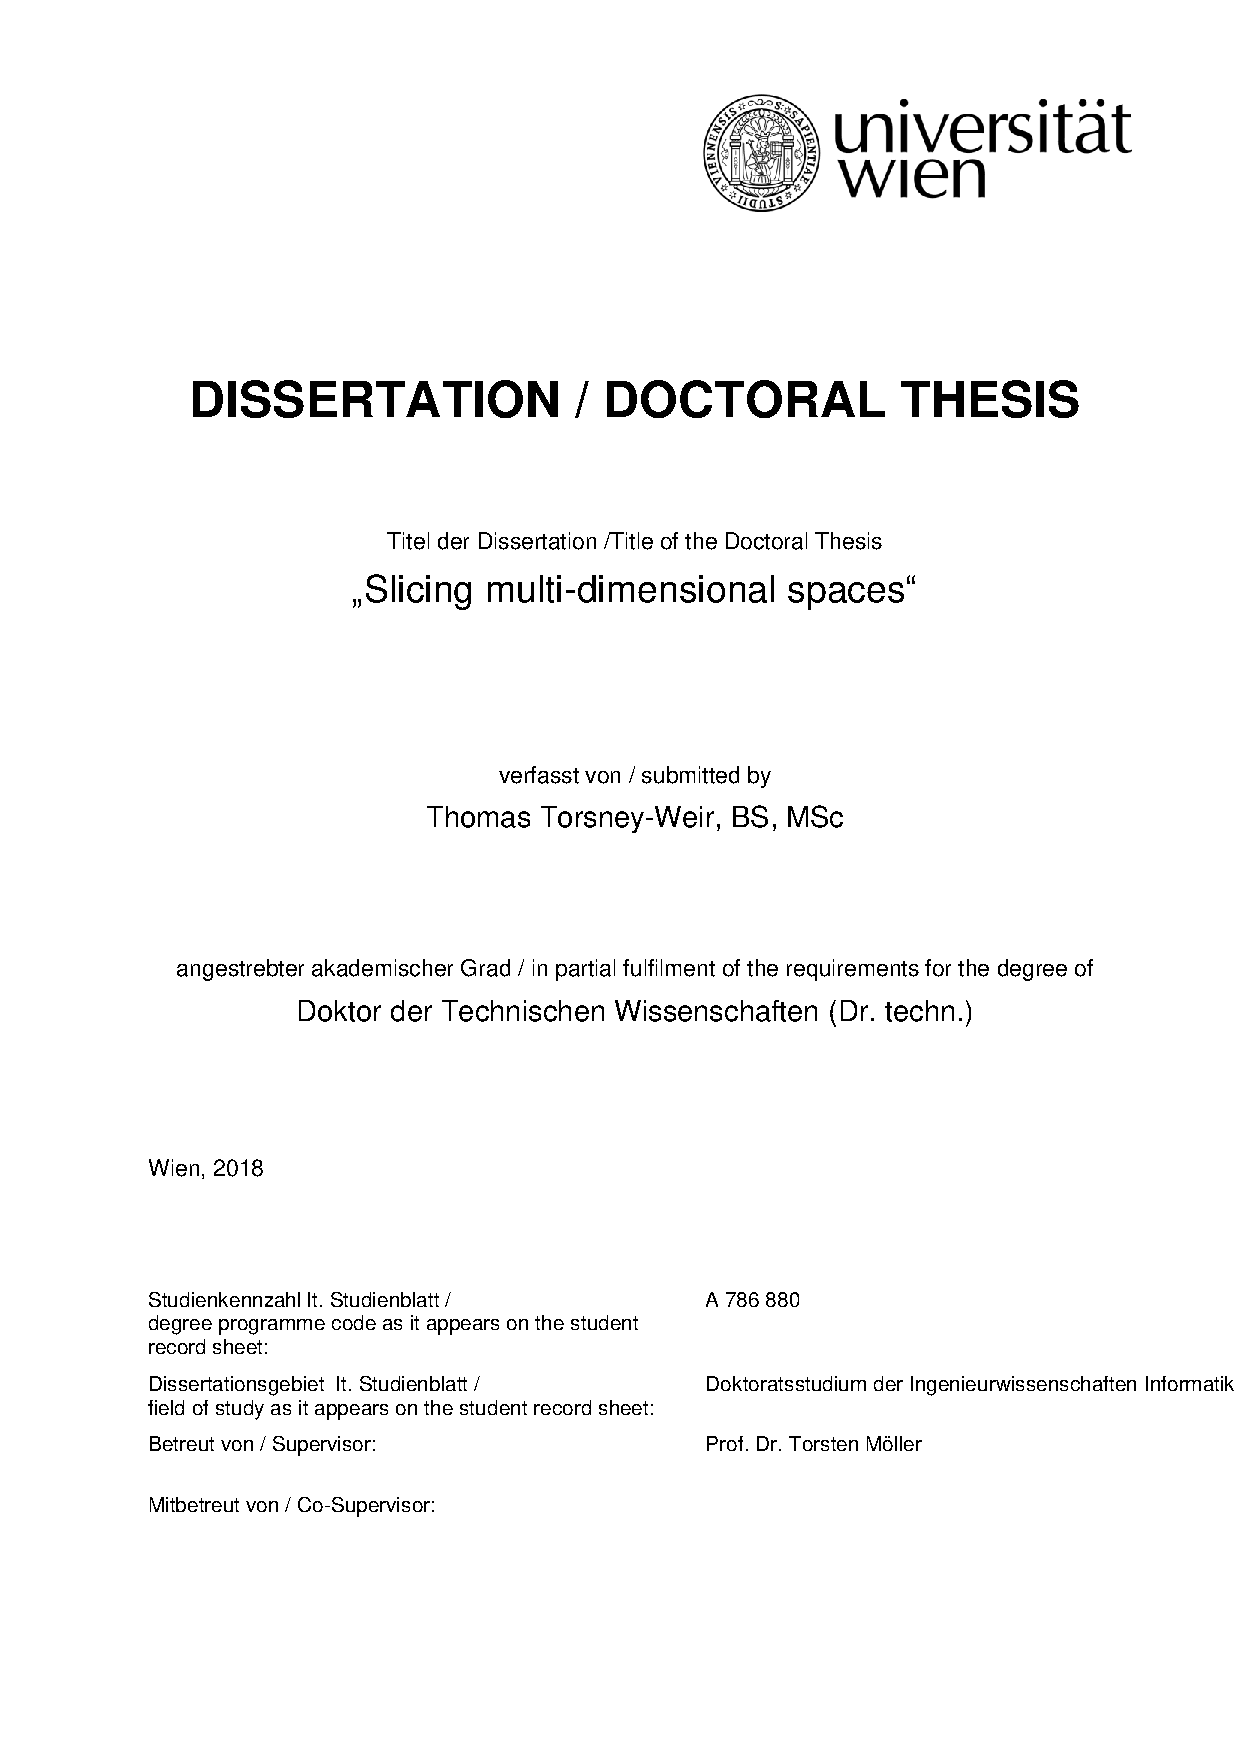
\includepdf[pages={1}]{cover_page.pdf}
%
\includepdf[pages={1}]{cover_page2.pdf}

%\listoffixmes

\dedication{To whomever finds this}

%\acknowledgements
\chapter*{Acknowledgements}

I would like to acknowledge the invaluable support of my supervisor, Torsten
M{\"o}ller, as well as Michael Sedlmair. Their assistance and experience have
been invaluable these last five years.

In addition, I want to thank all past and present members of the Visualization
and Data Analysis reserach group at the University of Vienna. In particular, I
want to thank Johanna Schlereth, Michael Phillips, Alireza Ghane, Raphael
Sahann, Christoph Kralj, Bernhard Fr{\"o}ler, Mohsen Kamalzadeh, Hamid Younesy,
Elena Rudkowsky, Patrick Wolf, Manfred Klaffenb{\"o}ck, Chrtistoph Langer,
Peter Ruch, Jennifer Prengel, Monika Gregor, Michaela Parzer, and Anne Marie
Faisst. The discussions I've had over these past few years have been many and
varied. I want to thank all of them for their suggestions and assistance in
performing my research.

And last but certainly not least, I want to thank my family for their love,
support, and encouragement throughout my life. Without their support I would
not have left a lucrative but boring career in finance in order to become a
happy student again. Furthermore, I would not have made it through the
most difficult times of my PhD without their support.



\clearpage

% contents
\tableofcontents*
\clearpage
\listoffigures
\clearpage
\listoftables
\clearpage
\listofalgorithms
\addcontentsline{toc}{chapter}{List of Algorithms}
\clearpage

% let's go!
\mainmatter

\chapter{Motivation}
\label{chp:motivation}
%Thesis: Multi-dimensional spaces are better visualized through slice based views

We live in a three-dimensional world. 
Ourselves and what we can interact with are in three dimensions.
\ttwnote{bridge sentence}
The phenomena governing the world are described as continuous processes.
In order to learn about the world around us we need to study these processes.
We begin by studying function plots in high 
school\ttwnote{figure?}. These give an intuitive view of one-dimensional 
phenomena. 
By exploring the relationship
between an input factor
%(temperature, pressure, et cetera) 
and output,
%(the weather) 
we can build an understanding on the relationship between the two.
We can also compare one function plot to another. Visual inspection of these plots
allows us to see common patterns. We can use our pattern recognition ability
to quickly categorize these different plots into different types of function
behavior. These function plots can also be used to describe two-dimensional
phenomena where there are two input factors. In this case we can use the third
dimension or color encoding to show the function value \ttwnote{figure?}. 
From these plots we can also make general statements about the ``shapes'' of
the behavior like how ``peaky'' the function is or if it is monotonically
increasing. These shapes give us intuition into the underlying processes and
help us learn about the world\ttwnote{can I find a pattern recognition reference?}\ttwnote{or maybe a reference from gestalt principles about grouping shapes together?}.

However, we interact with many phenomena around us that are essentially
multi-dimensional in nature. For example, the weather in a certain location is
determined by the temperature, pressure, humidity, dew point, wind velocity,
and wind direction, among others. A change in any of these factors results in a
change in the weather. Each of these factors can be given a ``spatial
embedding.'' Then, they can be viewed as a dimension of some space.  By
``walking'' or navigating through this space we can observe the effect on the
weather due to changes in these parameters. 

Understanding multi-dimensional continuous spaces is difficult. As
three-dimensional beings we have real-world analogs for measurement,
angle, and position in three dimensions. We do not have these once we
move beyond three dimensions though. Nevertheless, visual analysis of
these multi-dimensional spaces has produced insights about the
underlying behavior~\cite{Sedlmair:2014}. The issue is how to show more
than three dimensions on a two-dimensional screen. 

One strategy is to discretize the dataset through sampling and then use the
wealth of discrete visualization tools available. Much of the work on
multi-dimensional data analysis developed from analysis of abstract data such
as tabular data\ttwnote{ref}. These datasets are often recorded from real-world
events such as census, species, or text data and contain many different aspects
about each entity. These datasets are inherently multi- or high-dimensional.
Each different aspect of the data items creates a dimension to be analyzed. For
example, census data consists of the address, age, marital status, among
others. In the case of these data the mental model is that of discrete objects
like humans, plants, or documents. Since the mental model is discrete in this
case it makes sense to use data processing and visualization tools designed for
discrete data.  However, our mental model is a continuous one. Therefore, the
discrete data paradigm breaks our mental model~\cite{Tory:2004a}. Rather, we
should use visualization techniques purpose-built for continuous data.

While not as
extensively developed, there is previous work on visualizing multi-dimensional,
continuous data. These techniques can be broadly classified into projection,
topological, and slicing methods.  \ttwnote{put in chart from Jurgen's
presentation (projection vs dim reduction)?} Projection methods attempt to
distort the multi-dimensional object in order to view it on a two-dimensional
screen. With projection techniques we can preserve distance, direction, size,
or angles, but not all of 
these~\cite{Snyder:1987}. 
Depending on the
projection method, we may see radically different representations.  The issue
is that it is not clear from the resulting visualization what sort of
transformation was performed on the data.  Thus it can be difficult to
reconstruct the mental model of the multi-dimensional object.  One of the most
often seen multi-dimensional projection techniques is the Schlegel
diagram~\cite{schlegel} which picks a ``face'' of a polytope and projects the
remaining faces inside it. Thus this technique only works for 4D polytopes.
Topological methods search the continuous dataset for values of interest, such
as critical points or contours.  Topological visualization techniques also
suffer from the issue of unclear transformation. It is difficult to relate the
resulting visualization back to features in the multi-dimensional object.

Slice-based views of multi-dimensional continuous spaces have not been explored
as extensively as other options.  This work began with the advent of
HyperSlice~\cite{Wijk:1993}. HyperSlice provides the framework for visualizing
multi-dimensional continuous objects as a set of two-dimensional slices
(\autoref{fig:slicing_overview}). HyperSlice extends the idea of slicing
from medical imaging to any number of dimensions. There are $d \choose 2$
subpanels, one for each pair of dimensions. Each panel shows a 2D slice
of the object. The horizontal axis shows one dimension and the vertical 
axis shows another dimension. With 2D slices of solid multi-dimensional objects
color is often used to encode value. 

My work is inspired by the HyperSlice technique. Van Wijk and van Liere
introduced the idea of using slice-based views of multi-dimensional data.
However, they did not expand on what data types and tasks are involved in
multi-dimensional continuous data analysis.  I build on their work,
investigating the usefulness of slice-based views of continuous
multi-dimensional datasets. I also identified tasks involved in
multi-dimensional data analysis. These tasks informed the development of one-
and two-dimensional slice-based views.

In this thesis I will explore
the possibilities of these slice-based views. Through a number of case
study examples, I will demonstrate the power of these views and ways to
address their shortcomings.

\begin{figure}
  \centering
  %\includegraphics{slicing_overview}
  \label{fig:slicing_overview}
  \caption{
    \ttwnote[nomarginclue]{diagram of slicing}
  }
\end{figure}

%\tmnote{
%%- I think your reasoning though is not so much as looking at wheather. Rather,
%%I would argue that we have learned about the world through looking at 1D plot
%%in school or by comparing (and equating) things into classes of similar things
%%(hence, shape is a nice thing for us to reason about.
%- then you can talk about extending reasoning of 3D world to higher
%dimensions, that it is hard and all.
%- then I would argue about continuous vs. discrete. to me it is important to
%understand the mental model of how we reason about a phenomenon. somtimes
%discrete is important (some examples) sometimes continues (simulations,
%incluence of a parameter)
%- then you can reason about what Vis techniques we have for understanding
%cont. spaces
%}


\section{Multi-dimensional spaces}
\label{sec:motivation:multi-d}

There are a number of domains where one can apply the analysis of continuous
multi-dimensional data.  As of yet, there has not been a comprehensive data and
task analysis for multi-dimensional continuous data analysis. For discrete
data, there are several task 
analyses~\cite{Shneiderman:1996,Brehmer:2013,Amar:2004}. 
However, they are
focused on identifying and selecting particular data items. Continuous datasets
consist of ranges of values as well as functions. Functions can be seen as a
mapping from ranges of numbers to other ranges. The analysis task here is to
study these ranges.  Tasks addressing studying the mappings or studying the
relationship between ranges have not yet been covered by visualization task
analyses. Thus, there is no comprehensive source for what analysis tasks one
wants to perform given a continuous multi-dimensional dataset.  Work in this
area has traditionally focused on developing a specific visualization for a
specific task. For example, topological spines extracts critical points from a
scalar field~\cite{Correa:2011}. One goal of this thesis is to develop this
task taxonomy for visualization of continuous multi-dimensional data.

%Often work on continuous multi-dimensional data analysis is done in the context
%of design studies~\cite{Sedlmair:2012}. The issue is transferability, while
%important, is not always considered. 

%Each of these application scenarios are often treated individually. These all
%fit under a unified visualizaiton method though.

These domains can be broadly classified into two types based on their analysis
tasks. One type, \emph{manifold} analysis, deals with understanding the
relationship between inputs and outputs. This is a functional relationship.
The user wants to inspect how changes in the inputs (independent variables)
affect the outputs (dependent variables). One can also perform \emph{shape}
analysis. Here, in terms of the analysis tasks, there is no identification of
independent and depdendent variables. We look at each of these in turn.

\subsection{Manifolds}
\label{sec:manifolds}

Studying the mapping between continuous ranges means studying functional
relationships and thus manifolds.  The critical issue is understanding the
relationship between independent and dependent variables.  Subtasks in manifold
analysis include examining critical points, assessing the sensitivity of
parameters, and understanding the shape of the manifold.  Analyzing functions
is of course within the realm of manifold analysis.  Another area where
understanding the manifold is important is analyzing optimization surfaces and
functions.  In this case, the identification of extrema is important for
understanding how many and the relative location of local optima. In addition,
we want to understand the degree to which these are extrema. These can result
in global optimization algorithms ``getting stuck'' in local optima rather than
continuing to search for the global optimum. Optimization algorithms need to be
carefully tuned to properly detect these features and ignore them where
necessary.

Simulations can be used to run experiments that are impractical or impossible
in the real world.  Simulation analysis is another area where the analysis
tasks, in the abstract, is examining functions. If we look back at the weather
simulation from before, the inputs to the function are things like the
temperature and pressure.  The output is, for example, the likelihood of rain
the next day. The function is the simulation itself. Computer simulations are
deterministic.  A deterministic simulation has a mapping from each unique input
parameter configuration to an output value. This is the same as a functional
relationship. The sensitivity and extrema are also important to simulation
analysis.  Thus, these can all be analyzed with visualizations of a manifold.

%Some computer simulations are considered stochastic. That is, their output
%is the determined by a random number generator as well as input values.
%Stochastic simulations can be converted to deterministic by treating the 
%random number generator seed as another parameter.

To date, manifold visualizations have concentrated on a particular analysis
task or a particular application domain. For example, visualizations of the
Morse-Smale complex~\cite{MSvis} are focused on showing only critical points of
the manifold. As with any visualization designed for a specific task, they must
be used in combination with other views for visual analysis of domain-specific
data. Domain-specific visualizations often used linked views to show different
aspects of data to accomplish multiple tasks at once. However, they are purpose
built for a specific domain. While techniques may transfer from one domain to
another~\cite{Seldmair:2012}, it is not always clear how.
My goal is to unify these methods to a certain extent.
As I will show in \autoref{chp:sliceplorer}, slice-based views of manifolds
can be used for a wide variety of tasks in a wide number of domains.

\subsection{Shapes}
\label{sec:shapes}

One may also want to understand the relationship or correlation between
multiple continuous values. This is in contrast to studying the relationship
between independent and dependent variables in the manifold case. In this case
we want to study the relationship of all variables. Careful study of the shape
of the dataset can give insight into the relationship between the various
ranges of dimensions of the object. For example, one may want to know if the
overall shape is a sphere, donut, or box. In addition one may be interested in
any kinks or cusps in the dataset. \ttwnote{why?} These do not necessarily need
to be true cusps. Changes in the gradient and curvature of the shape are also
of great interest.

These analysis tasks of multi-dimensional shapes can be applied to a number of
different areas. The study of polytopes is one such area and perhaps the most
direct application of understanding multi-dimensional continuous shapes.
Polytopes are the multi-dimensional generalization of polyhedra and polygons.
The tasks are to understand the symmetries and patterns making up the
polytopes~\cite{Ziegler:2012}. Perhaps a less obvious connection is the
analysis of the tradeoff curves in multi-objective optimization. Since we are
performing optimization we are interested in the tradeoffs amongst all the
non-dominated points~\cite{Kung:1975}. This is also known as the Pareto
front. In this case, the user wants to understand what are the costs of
reducing one or more parameters in order to increase the value of others. Cusps
or large changes in curvature in these datasets are important since they show
fundamental changes in the rate of tradeoff.  With a proper view of a
multi-dimensional object we can also view differences betweeen two objects
directly. With 1-, 2-, or 3-D objects we show these differences directly and
can understand them.  Showing a difference object requires the user to reconstruct
the two objects at once. This requires quite a lot of mental processing.
However, the two-stage processing of showing a difference object and then
performing dimension reduction makes it difficult to view difference objects
with dimension reduction. Slicing, as a direct visualization technique, does
not have this problem. \ttwnote{confusing, use images/diagrams to explain?}

These two different data types and sets of tasks require different visualization
considerations. Proper visualization for manifold analysis should focus on
the relationships between independent and dependent variables. Visualizations
of shapes do not have this mapping requirement and instead focus on the 
relationships between dimensions. With this categorization in mind, we can now
examine the available visualization techniques to examine these.



\section{Mental models}
\label{sec:mental_models}

\ttwwarning{write}

Mental models~\cite{Liu:2010a}
\cite{McNeil:2015}

\begin{itemize}
\item what about discrete data?
\item why is this important?
\item issue: ranges - why? where do they come from?
\item issue: treating dimensions equally
\item issue: understanding mapping relationships
\end{itemize}



\section{Visualizing multi-dimensional continuous spaces}
\label{sec:multi-d-challenges}

Understanding multi-dimensional space is difficult. As humans, we simply do not
have the spatial analogs in more than three dimensions. A number of methods
have been developed to extract specific features from the multi-dimensional
object. For example, when studying polytopes, the number of faces and
symmetries is very important~\cite{Ziegler:2012}. However, these only produce
an answer without sufficient context. They do not necessarily give any
intuition as to how to transfer our three-dimensional knowledge to
multi-dimensional spaces.

%\ttwnote{how visualization can help}
%\ttwnote{some sort of insight generation from context?}

Visualizations of multi-dimensional spaces on a 2D screen must contend with
some sort of reduction of the information. A proper visualization must select
visual encodings that highlight the information we want to see. Any sort of
data reduction requires trade-offs. The best visualization choices acknowledge
any difficiencies to a particular visual encoding. By acknowledging these
difficiencies, we can design tools to compensate for their shortcomings while
still maintaining their advantages. Therefore, it is worth first looking at the
possible mappings of data to visual elements. Then, I present commonly used
visual encodings of multi-dimensional continuous data using these mappings.

\subsection{Encoding multi-dimensional data}

Multi-dimensional continuous data consists of a set of continuous ranges, one
for each dimension. In the case of manifold analysis, each of these ranges can
be additionally classified as ``dependent'' or ``independent'' depending on
which side of the mapping they are on. Typical visualization practice is to
give each dimension a separate visual channel. There are a number of possible
visual channels that have been identified.  The ranking of effectiveness of
visual channels (shown in \autoref{tbl:visual_encodings}) was proposed by
Bertin~\cite{Bertin:1967} and confirmed through experiments by Cleveland and
McGill~\cite{Cleveland:1984}, Mackinlay~\cite{Mackinlay:1986}, and Heer and
Bostock~\cite{Heer:2010}.  Munzner~\cite{Munzner:2014} provides a summary of
the results. We are also limited in how many channels we can use
simulataneously. According to Ware~\cite{Ware:2004}, certain channels, such as
red and green are not visually seperable. 

\begin{table}
  \caption{Rankings of visual encodings of quantiative data}
  \label{tbl:visual_encodings}
  \begin{tabular}{llll}
    \cite{Bertin:1967} & \cite{Cleveland:1984} & \cite{Mackinlay:1986} & \cite{Munzner:2014} \\
     Position & Position along a common scale & Position & Position on common scale \\
     Size & Position along identical, nonaligned scales & Length & Position on unaligned scale \\
     (Grey) Value & Length & Angle & Length (1D size) \\
     Texture & Direction & Slope & Tilt/angle \\
     Color & Angle & Area & Area (2D size) \\
     Orientation & Area & Volume & Depth (3D position) \\
     Shape & Volume & Density & Color luminance\\
     & Curvature & Color saturation & Color saturation \\
     & Densities & Color hue & Curvature \\
     & Shading & & Volume (3D size) \\
     & Color saturation &           & 
  \end{tabular}
\end{table}

The difficulty of visualizing a continuous multi-dimensional space on a
two-dimensional screen brings a number of challenges. We treat each dimension
separately, thus, we need several different visual channels. However, there are
simply not enough visual channels available to draw a 15-dimensional object in
a single view. This is further complicated by the fact that separate visual
channels are not necessarilly visually seperable.  Furthermore, each dimension
of the multi-dimensional object under study is treated equally. For example, no
particular axis of a polytope is more important than any other.  We should
encode each dimension using equally weighted effectiveness channels.  With
fewer channels available than data dimensions we either need to reduce the data
or use multiple views to properly visualize the data.


\subsection{Methods}

The common taxonomy of how to view multi-dimensional data on screen is based on
discrete data analysis. There, there are two categories: dimension reduction or
projection. With continuous data, though there is a third possibility, that of
slicing. Therefore, I view the taxonomy of \emph{continuous} multi-dimensional
data analysis methods into two categories. Data-driven methods include both
projection and dimension reduction and reduce the dimensionality of the data
before visualization. View-based methods reduce the data during the
visualization. Slicing is a view-based method.

Purely data-driven methods are commonly known as feature selection or dimension
reduction. The goal is to find a subset of dimensions that are critical to
understanding the dataset. Topological techniques take this a step further.
They discard all spatial information about the dataset and only concentrate on
the difference in function value, as in the Morse-Smale
complex~\cite{Gyulassy:2012a}, or evolution of contours, as in the contour
tree~\cite{Carr:2003a}.  Projections also synthesize the dataset into new
dimensions to show using visual channels. Principal component
analysis~\cite{Holbrey:2006} is a popular choice in this area. This rotates the
space and thus produces new set of dimensions that are a linear combination of
the input dimensions. Even this relatively simple operation (a rotation) can be
difficult to understand. For example, iPCA~\cite{Jeong:2009a} was a tool to
help users understand the effects of the dimensional transformation.

View-based methods try and produce multiple linked views of a multi-dimensional
dataset from different angles. Each view shows a subset of the dimensions.
This way we can use a proper set of visual channels for each view.  We use
interaction to link these different views. These multiple, coordinated, linked
views have been one of the biggest success stories from the visualization
community~\cite{Rao:1994}. The traditional HyperSlice~\cite{Wijk:1993}
technique falls into this category. Each panel of the HyperSlice view shows two
of the input dimensions and the value is encoded with color.
The views are linked through the focus point selection. Changing the focus point
in one sub-plot updates the other sub-plots.

My work focuses on the exploration of the combination of data-driven and
view-based methods.  Data-driven methods reduce the data in a way that we can
get a global overview of the dataset. View-based methods are much more detailed
but can only produce a local view of the data. By combining these methods I can
achieve both a global overview as well as an on-demand local view of the
dataset in a single visualization. 



\section{Slices}
\label{sec:slicing-advantages}

Slicing offers a number of advantages over other multi-dimensional
visualization techniques. Slicing is a direct visualization of the
multi-dimensional object. In contrast to methods like projection or dimension
reduction, slicing does not distort the dimensions in order to display them on
a two-dimensional screen. Since there is no distortion, distances in the visual
representation are directly proportional to distances in the object. This is
one of the reasons that slicing is popular in the medical imaging community.
Sizes of organs or tumors can be measured visually on screen. Additionally,
relative sizes correspond to what a doctor would expect to see in the body.
Multi-dimensional data is abstract. It lacks the correspondence to real-world
objects that the medical community uses to understand their two- and
three-dimensional datasets. Nevertheless, it is still important in
multi-dimensional data analysis to properly estimate distances and relative
sizes. 
\ttwnote{example}

Another benefit of the direct visualization is that users do not require
extensive training to understand the visualization. The concept of slicing
through a three-dimensional object is a familiar one. Humans are used to this
even from cooking. This concept of slicing can be extended from this 
well-known metaphor to cover multiple slices of multi-dimensional objects.

Slice views use the horizontal and vertical axes for showing the effects due to
the input parameters. These axes are the most perceptually
uniform~\cite{Stevens:1957} and are considered the most effective
(\autoref{tbl:enc_effectiveness}). One- or two-dimensional
plots are replicated for each combination of dimensions in order to show more
than two dimensions at once. This promotes familiarity of the visualization.
Once the user has learned to read a single panel, they can apply this knowledge
to the remaining panels. This approach follows the principal of small
multiples~\cite{Archambault:2011}. \ttwnote{maybe move this to a section on
general vis techniques}

In order to produce a slice plot one needs to first pick a particular
\emph{focus point} in the multi-dimensional space. This focus point determines
which slices are being viewed. Selecting a good focus point a-priori is
difficult. 
\ttwnote{from michael: this is a challenge again. imho it might be clearer to list all challenges in the same spot. I always liked the spectrum between toplogical approaches and Hyperslices. Then you can say that your goal is to combine their benefits and reduce their weaknesses and how you address these challenges.}
It either requires a great deal of luck or careful analysis of the
dataset. This is not always possible. Slice-based views require some sort of
interactive focus point selection. Interactively browsing through the slices
requires interaction controls to give the user control over the focus point.
Furthermore, we need some kind of navigation map to show which focus points the
user has selected so that they do not become lost. Neither of these navigation
aids are well developed at this point. This need for interaction is likely one
of the reasons that slice-based views have not developed as much as projection
or topological techniques. Static views are much easier to include in papers
and don't require explanation prior to use.

The other implementation issue of slice-based views is ensuring that the
visualization can remain interactive. In this case, interactive is defined as
the rate at which the user can maintain their
concentration~\cite{Shneiderman:1987}. This is often defined at 10 frames per
second. It can be difficult to compute a 2D slice of an arbitrary complex
multi-dimensional object. 






\section{Upcoming}
\label{sec:thesis_outline}

\ttwnote{expand}
In my own work, I address these two critical issues. The navigation issue can
be solved with sampling. With both Sliceplorer (\autoref{chp:sliceplorer}) and
HyperSliceplorer (\autoref{chp:hypersliceplorer}), I sample over a number of
focus points and display them all at once. In \autoref{chp:rendering}, I
discuss how we can take advantage of the multi-dimensional geometry to allow
interactive-speed browsing of the focus points. My goal is to highlight the
advantages of slice-based methods for multi-dimensional data analysis. At the
same time I want to address the limitations. The end goal is to bring
slice-based views into the standard toolbox of visualizations.





\chapter{1D slices}
\label{chp:sliceplorer}

\begin{figure}
  \centering
  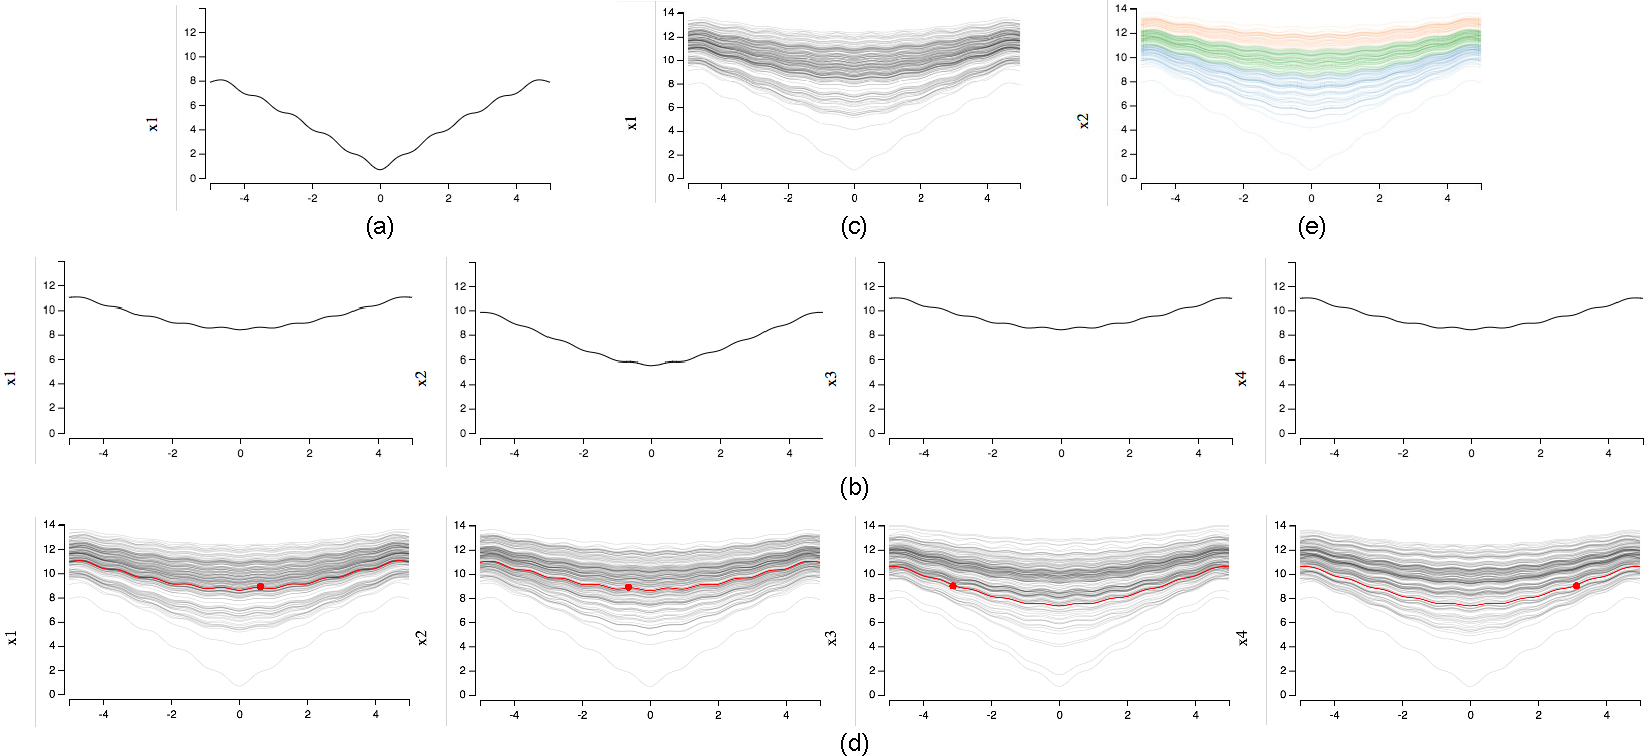
\includegraphics[width=0.9\textwidth]{sliceplorer_overview.pdf}
  \caption{
    The evolution of Sliceplorer. I adapt the commonly known technique of
    1D function plots (a) to
    multiple dimensions by taking a small multiples approach and repeating each
    plot for each dimension (b). I address the
    focus point selection problem by sampling over the parameter space and then
    projecting the slices in the corresponding plot
    (c). The user can mouse over a particular
    slice in one plot and the corresponding slices are highlighted in the other
    dimension plots (d). This allows one to
    see the corresponding function behaviors in the other dimensions.  Finally,
    one can cluster the function slices (e), to
    show groups of similar behavior in the manifold.
  }
  \label{fig:walkthrough}
\end{figure}

First, we turn to the visual exploration of multi-dimensional continuous
functions. In this case, the user is primarily interested in the relationship
between dependent and independent variables. In this chapter, I discuss how
one-dimensional slices can be a highly intuitive way of visualizing
multi-dimensional manifolds. I also discuss how we can use projections of 
slices to address the focus point selection issue. The task analysis in this
chapter goes into detail about what sort of tasks one wants to perform when 
visualizing manifolds.


%Thesis: Multi-dimensional spaces are better visualized through slice based views

We live in a three-dimensional world.  Ourselves and what we can interact with
are in three dimensions.  We learn about our world by studying the various
phenomena around us.  These phenomena are described as continuous processes.
In the beginning of our  education we study function plots in high school.
These give an intuitive view of one-dimensional phenomena.  By exploring the
relationship between an input factor
and output,
we can build an understanding on the relationship between the two.  We can also
compare one function plot to another. Visual inspection of these plots allows
us to see common patterns. We use our pattern recognition ability to quickly
categorize these different plots into different types of function behavior.
Function plots can also be used to describe two-dimensional phenomena. These
show the effect due to two input factors. In this case we can use the third
dimension or color encoding to show the function value.  From these plots we
can also make general statements about the ``shapes'' of the behavior like how
``peaky'' the function is or if it is monotonically increasing. These shapes
give us intuition into the underlying processes and help us learn about the
world~\cite{Palmer:1999}.

We also interact with many phenomena around us that are essentially
multi-dimensional in nature. For example, the weather in a certain location is
determined by the temperature, pressure, humidity, dew point, wind velocity,
and wind direction, among others. A change in any of the factors results in a
change in the weather. Each of these factors can be given a ``spatial
embedding.'' Then, they can be viewed as a dimension of some space.  By
``walking'' or navigating through this space we can observe the effect on the
weather due to changes in these parameters. 

Understanding multi-dimensional continuous spaces is difficult. As
three-dimensional beings we have real-world analogs for measurement, angle, and
position in three dimensions. We do not have these once we move beyond three
dimensions though. Nevertheless, visual analysis of these multi-dimensional
spaces has produced insights about the underlying
behavior~\cite{Sedlmair:2014,Gleicher:2016}. The issue is how to show more than
three dimensions on a two-dimensional screen. 

One strategy is to discretize the dataset through sampling and then use the
wealth of discrete visualization tools available. Much of the work on
multi-dimensional data analysis developed from analysis of 
tabular data. These datasets are often recorded from real-world
events such as census, species, or text data and contain many different aspects
about each entity. Thus, these datasets are inherently multi- or high-dimensional.
Each different aspect of the data items creates a dimension to be analyzed. 
In the case of these data the mental model is that of discrete objects
like humans, plants, or documents. Since the mental model is discrete in this
case it makes sense to use data processing and visualization tools designed for
discrete data.  However, our mental model for physical data is a continuous 
one. Therefore, the
discrete data paradigm breaks our mental model~\cite{Tory:2004a,Liu:2010a}. 
Breaking the mental model means that the visualization is not conveying the
complexities of the continuous phenomena.
Rather, we
should use visualization techniques purpose-built for continuous data.

While not as
extensively developed, there is previous work on visualizing multi-dimensional,
continuous data. These techniques can be broadly classified into projection,
topological, and slicing methods.  
Projection methods attempt to
distort the multi-dimensional object in order to view it on a two-dimensional
screen. With projection techniques we can preserve distance, direction, size,
or angles, but not all of 
these~\cite{Snyder:1987}. 
Depending on the
projection method, we may see radically different representations.  The issue
is that it is not clear from the resulting visualization what sort of
transformation was performed on the data.  Thus it can be difficult to
reconstruct the mental model of the multi-dimensional object.  One of the most
often seen multi-dimensional projection techniques is the Schlegel
diagram~\cite{Sommerville:1929} which picks a ``face'' of a polytope and projects the
remaining faces inside it. Thus, this technique only works for 4D polytopes.
Topological methods search the continuous dataset for values of interest, such
as critical points or contours.  Topological visualization techniques also
suffer from the issue of unclear transformation. It is difficult to relate the
resulting visualization back to features in the multi-dimensional object.

Slice-based views of multi-dimensional continuous spaces have not been explored
as extensively as other options.  This work began with the advent of
HyperSlice~\cite{Wijk:1993}.  HyperSlice extends the idea of slicing from
medical imaging to any number of dimensions.  HyperSlice provides the framework
for visualizing multi-dimensional continuous objects as a set of
two-dimensional slices.  There are $d \choose 2$ subpanels, one for each pair
of dimensions. Each panel shows a 2D slice of the object. The horizontal axis
shows one dimension and the vertical axis shows another dimension. Essentially,
each sub-plot of HyperSlice shows a 2D function plot. With 2D slices of solid
multi-dimensional objects color is often used to encode value. 

My work is inspired by the HyperSlice technique. Van Wijk and van Liere
introduced the idea of using slice-based views of multi-dimensional data.
However, they did not expand on what data types and tasks are involved in
multi-dimensional continuous data analysis.  I build on their work,
investigating the usefulness of slice-based views of continuous
multi-dimensional datasets. I also identified tasks involved in
multi-dimensional data analysis. The task analysis informed the development of
one- and two-dimensional slice-based views.

In this thesis I will explore
the possibilities of these slice-based views. Through a number of case
study examples, I will demonstrate the power of these views and ways to
address their shortcomings.

\subsection{Multi-dimensional spaces}
\label{sec:motivation:multi-d}

There are a number of domains where one can apply the analysis of continuous
multi-dimensional data.  As of yet, there has not been a comprehensive data and
task analysis for multi-dimensional continuous data analysis. For discrete
data, there are several task 
analyses~\cite{Shneiderman:1996,Brehmer:2013,Amar:2004}. 
However, they are
focused on identifying and selecting particular data items. Continuous datasets
consist of ranges of values as well as functions. Functions can be seen as a
mapping from ranges of numbers to other ranges. The analysis task here is to
study these ranges, their relationships to each other, and the mappings between
them. Tasks addressing these
have not yet been covered by visualization task analyses. Thus,
there is no comprehensive source for what analysis tasks one wants to perform
given a continuous multi-dimensional dataset.  Work in this area has
traditionally focused on developing a specific visualization for a specific
task. For example, topological spines extracts critical points from a scalar
field~\cite{Correa:2011}. One goal of this thesis is to develop this task
taxonomy for visualization of continuous multi-dimensional data.


These domains can be broadly classified into two types based on their analysis
tasks. One type, \emph{manifold} analysis, deals with understanding the
relationship between inputs and outputs. This is a functional relationship.
The user wants to inspect how changes in the inputs (independent variables)
affect the outputs (dependent variables). One can also perform \emph{shape}
analysis. Here, in terms of the analysis tasks, there is no identification of
independent and dependent variables. We look at each of these two in turn.

\subsection{Manifolds}
\label{sec:manifolds}

Studying the mapping between continuous ranges means studying functional
relationships and thus manifolds.  The critical issue is understanding the
relationship between independent and dependent variables.  Subtasks in manifold
analysis include examining critical points, assessing the sensitivity of
parameters, and understanding the shape of the manifold.  
One area where
understanding the manifold is important is analyzing optimization surfaces and
functions.  In this case, the identification of extrema is important for
understanding how many and the relative location of local optima. In addition,
we want to understand the degree to which these are extrema. These can result
in global optimization algorithms ``getting stuck'' in local optima rather than
continuing to search for the global optimum. Optimization algorithms need to be
carefully tuned to properly detect these features and ignore them where
necessary.

Simulations can be used to run experiments that are impractical or impossible
in the real world.  Simulation analysis is another area where the analysis
tasks, in the abstract, are examining functions. If we look back at the weather
simulation from before, the inputs to the function are things like the
temperature and pressure.  The output is, for example, the likelihood of rain
the next day. The function is the simulation itself. Computer simulations are
deterministic.  A deterministic simulation has a fixed mapping from each unique
input parameter configuration to an output value. This is the same as a
functional relationship. The sensitivity and extrema are also important to
simulation analysis.  Thus, these can all be analyzed with visualizations of a
manifold.

To date, manifold visualizations have concentrated on a particular analysis
task or a particular application domain. For example, visualizations of the
Morse-Smale complex~\cite{Gerber:2010} are focused on showing only critical
points of the manifold. As with any visualization designed for a specific task,
they must be used in combination with other views for visual analysis of
domain-specific data. Domain-specific visualizations often used linked views to
show different aspects of data to accomplish multiple tasks at once. However,
they are purpose built for a specific domain. While techniques may transfer
from one domain to another~\cite{Sedlmair:2012}, it is not always clear how.
My goal is to unify these methods to a certain extent.  As I will show in
\autoref{chp:sliceplorer}, slice-based views of manifolds can be used for a
wide variety of tasks in a wide number of domains.

\subsection{Shapes}
\label{sec:shapes}

One may also want to understand the relationship or correlation between
multiple continuous values. In the manifold analysis case we have the notion
of independent and dependent variables. This classification does not exist 
here.
In this case
we want to study the relationship of all variables. Careful study of the shape
of the dataset can give insight into the relationship between the various
ranges of dimensions of the object. For example, one may want to know if the
overall shape is a sphere, donut, or box. In addition one may be interested in
any kinks or cusps in the dataset. Changes in the gradient and curvature of
the shape are also of great interest. These indicate changes in correlation or
relation.

The analysis tasks of multi-dimensional shapes can be applied to a number of
different areas. The study of polytopes is one such area and perhaps the most
direct application of understanding multi-dimensional continuous shapes.
Polytopes are the multi-dimensional generalization of polyhedra and polygons.
The tasks are to understand the symmetries and patterns making up the
polytopes~\cite{Ziegler:2012}. Perhaps a less obvious connection is the
analysis of the tradeoff curves in multi-objective optimization. Since we are
performing optimization we are interested in the tradeoffs amongst all the
non-dominated points~\cite{Kung:1975}. This is also known as the Pareto
front. In this case, the user wants to understand what are the costs of
reducing one or more parameters in order to increase the value of others. Cusps
or large changes in curvature in these datasets are important since they show
critical changes in the rate of tradeoff.  With a proper view of a
multi-dimensional object we can also view differences between two objects
directly. 

These two different data types and sets of tasks require different visualization
considerations. Proper visualization for manifold analysis should focus on
the relationships between independent and dependent variables. Visualizations
of shapes do not have this mapping requirement and instead focus on the 
relationships between dimensions. With this categorization in mind, we can now
examine the available visualization techniques to examine these.


\subsection{Visualizing multi-dimensional continuous spaces}
\label{sec:multi-d-challenges}

Understanding multi-dimensional space is difficult. As humans, we simply do not
have the spatial analogs in more than three dimensions. A number of methods
have been developed to extract specific features from the multi-dimensional
object. For example, when studying polytopes, the number of faces and
symmetries is very important~\cite{Ziegler:2012}. However, these only produce
an answer without sufficient context. They do not necessarily give any
intuition as to how to transfer our three-dimensional knowledge to
multi-dimensional spaces.

Visualizations of multi-dimensional spaces on a 2D screen must contend with
some sort of reduction of the information. A proper visualization must select
visual encodings that highlight the information we want to see. Any sort of
data reduction requires trade-offs. The best visualization choices acknowledge
any deficiencies to a particular visual encoding. By acknowledging these
deficiencies, we can design tools to compensate for their shortcomings while
still maintaining their advantages. Therefore, it is worth first looking at the
possible mappings of data to visual elements. Then, I present commonly used
visual encodings of multi-dimensional continuous data using these mappings.

\subsection{Encoding multi-dimensional data}

Multi-dimensional continuous data consists of a set of continuous ranges, one
for each dimension. In the case of manifold analysis, each of these ranges can
be additionally classified as ``dependent'' or ``independent'' depending on
which side of the mapping they are on. Typical visualization practice is to
give each dimension a separate visual channel. There are a number of possible
visual channels that have been identified.  The ranking of effectiveness of
visual channels (shown in \autoref{tbl:visual_encodings}) was proposed by
Bertin~\cite{Bertin:1967} and confirmed through experiments by Cleveland and
McGill~\cite{Cleveland:1984}, Mackinlay~\cite{Mackinlay:1986}, and Heer and
Bostock~\cite{Heer:2010}.  Munzner~\cite{Munzner:2014} provides a summary of
the results. We are also limited in how many channels we can use
simultaneously. According to Ware~\cite{Ware:2004}, certain channels, such as
red and green are not visually separable. 

\begin{table}
  \caption{Rankings of visual encodings of quantitative data}
  \label{tbl:visual_encodings}
  \begin{adjustbox}{max width=\linewidth}
  \begin{tabular}{llll}
    Bertin~\cite{Bertin:1967} & Cleveland and McGill~\cite{Cleveland:1984} & Mackinlay~\cite{Mackinlay:1986} & Munzner~\cite{Munzner:2014} \\
    \hline \\
     Position & Position along a common scale & Position & Position on common scale \\
     Size & Position along identical, nonaligned scales & Length & Position on unaligned scale \\
     (Grey) Value & Length & Angle & Length (1D size) \\
     Texture & Direction & Slope & Tilt/angle \\
     Color & Angle & Area & Area (2D size) \\
     Orientation & Area & Volume & Depth (3D position) \\
     Shape & Volume & Density & Color luminance\\
     & Curvature & Color saturation & Color saturation \\
     & Densities & Color hue & Curvature \\
     & Shading & & Volume (3D size) \\
     & Color saturation &           & 
  \end{tabular}
  \end{adjustbox}
\end{table}

The difficulty of visualizing a continuous multi-dimensional space on a
two-dimensional screen brings a number of challenges. We treat each dimension
separately, thus, we need several different visual channels. However, there are
simply not enough visual channels available to draw a 15-dimensional object in
a single view. This is further complicated by the fact that separate visual
channels are not necessarily visually separable.  Furthermore, each dimension
of the multi-dimensional object under study is treated equally. For example, no
particular axis of a polytope is more important than any other.  We should
encode each dimension using equally weighted effectiveness channels.  With
fewer channels available than data dimensions we either need to reduce the data
or use multiple views to properly visualize the data.


\subsection{Methods}

The common taxonomy of how to view multi-dimensional data on screen is based on
discrete data analysis. There, there are two categories: dimension reduction or
projection. With continuous data, though there is a third possibility, that of
slicing. Therefore, I view the taxonomy of \emph{continuous} multi-dimensional
data analysis methods into two categories. Data-driven methods include both
projection and dimension reduction and reduce the dimensionality of the data
before visualization. View-based methods reduce the data during the
visualization. Slicing is a view-based method.

Purely data-driven methods are commonly known as feature selection or dimension
reduction. The goal is to find a subset of dimensions that are critical to
understanding the dataset. Topological techniques take this a step further.
They discard all spatial information about the dataset and only concentrate on
the difference in function value, as in the Morse-Smale
complex~\cite{Gyulassy:2012a}, or evolution of contours, as in the contour
tree~\cite{Carr:2003a}.  Projections also synthesize the dataset into new
dimensions to show using visual channels. Principal component
analysis~\cite{Holbrey:2006} is a popular choice in this area. This rotates the
space and thus produces new set of dimensions that are a linear combination of
the input dimensions. Even this relatively simple operation (a rotation) can be
difficult to understand. For example, iPCA~\cite{Jeong:2009a} was a tool to
help users understand the effects of the dimensional transformation.

View-based methods try and produce multiple linked views of a multi-dimensional
dataset from different angles. Each view shows a subset of the dimensions.
This way we can use a proper set of visual channels for each view.  We use
interaction to link these different views. These multiple, coordinated, linked
views have been one of the biggest success stories from the visualization
community~\cite{Rao:1994}. The traditional HyperSlice~\cite{Wijk:1993}
technique falls into this category. Each panel of the HyperSlice view shows two
of the input dimensions and the value is encoded with color.
The views are linked through the focus point selection. Changing the focus point
in one sub-plot updates the other sub-plots.

My work focuses on the exploration of the combination of data-driven and
view-based methods.  Data-driven methods reduce the data in a way that we can
get a global overview of the dataset. View-based methods are much more detailed
but can only produce a local view of the data. By combining these methods I can
achieve both a global overview as well as an on-demand local view of the
dataset in a single visualization. 


\subsection{Slices}
\label{sec:slicing-advantages}

Slicing offers a number of advantages over other multi-dimensional
visualization techniques. Slicing is a direct visualization of the
multi-dimensional object. In contrast to methods like projection or dimension
reduction, slicing does not distort the dimensions in order to display them on
a two-dimensional screen. Since there is no distortion, distances in the visual
representation are directly proportional to distances in the object. This is
one of the reasons that slicing is popular in the medical imaging community.
Sizes of organs or tumors can be measured visually on screen. Additionally,
relative sizes correspond to what a doctor would expect to see in the body.
Multi-dimensional data is abstract. It lacks the correspondence to real-world
objects that the medical community uses to understand their two- and
three-dimensional datasets. Nevertheless, it is still important in
multi-dimensional data analysis to properly estimate distances and relative
sizes. 

Another benefit of the direct visualization is that users do not require
extensive training to understand the visualization. The concept of slicing
through a three-dimensional object is a familiar one. Humans are used to this
even from slicing fruits and vegetables with a knife. This concept of slicing
can be extended from this well-known metaphor to cover multiple slices of
multi-dimensional objects.

Slice views use the horizontal and vertical axes for showing the effects due to
the input parameters. These axes are the most perceptually
uniform~\cite{Stevens:1957} and are considered the most effective
(\autoref{tbl:visual_encodings}). One- or two-dimensional
plots are replicated for each combination of dimensions in order to show more
than two dimensions at once. This promotes familiarity of the visualization.
Once the user has learned to read a single panel, they can apply this knowledge
to the remaining panels. This approach follows the principal of small
multiples~\cite{Archambault:2011}. 

In order to produce a slice plot one needs to first pick a particular
\emph{focus point} in the multi-dimensional space. This focus point determines
which slices are being viewed. Selecting a good focus point a-priori is
difficult. 
It either requires a great deal of luck or careful analysis of the
dataset. This is not always possible. Slice-based views require some sort of
interactive focus point selection. Interactively browsing through the slices
requires interaction controls to give the user control over the focus point.
Furthermore, we need some kind of navigation map to show which focus points the
user has selected so that they do not become lost. Neither of these navigation
aids are well developed at this point. This need for interaction is likely one
of the reasons that slice-based views have not developed as much as projection
or topological techniques. Static views are much easier to include in papers
and don't require explanation prior to use.

The other implementation issue of slice-based views is ensuring that the
visualization can remain interactive. In this case, interactive is defined as
the rate at which the user can maintain their
concentration~\cite{Shneiderman:1987}. This is often defined at 10 frames per
second. It can be difficult to compute a 2D slice of an arbitrary complex
multi-dimensional object. 


\subsection{Upcoming}
\label{sec:thesis_outline}

My goal is to highlight the advantages of slice-based methods for
multi-dimensional data analysis. At the same time I want to address the
limitations. The end goal is to bring slice-based views into the standard
toolbox of visualizations.

In \autoref{chp:sliceplorer}, I examine how to visualize manifolds using
slices. I present Sliceplorer which is a system to view one-dimensional slices
of multi-dimensional manifolds. I use projections of these one-dimensional
slices instead of showing one focus point at a time. I also go into detail
about the tasks one wants to perform with manifold analysis.

I extend the idea of projections of slices to the second dimension in
\autoref{chp:hypersliceplorer}.  I show how this can be used to effectively
visually analyze the shape of multi-dimensional data. In many cases, this data
is given as a simplical mesh. I introduce an algorithm to compute 2D slices of
this mesh.  Using this algorithm, I show how we can visually understand
datasets like Pareto fronts or polytopes.

Finally, in \autoref{chp:rendering}, I discuss how we can take advantage of the
multi-dimensional geometry and GPU architecture to allow interactive-speed
browsing of the focus points. In addition to this algorithm, I develop a method
that can predict the amount of time needed per element to draw one frame of the
visualization. I then show how this estimation formula can be calibrated to a
particular user's hardware.



\section{Related work}
\label{sec:related-work}

Multi-objective optimization and multi-dimensional objects are two areas
where it is important to study shapes in over three dimensions. We discuss 
these areas below. Topological techniques are based on viewing critical points
of manifolds~\cite{Correa:2011,Gerber:2010} or how contours merge and 
split~\cite{Carr:2003a}. We do not discuss them further. Manifold analysis
is very different than visualizing shapes. 

The need to understand multi-dimensional polytopes is apparent to 
geometers~\cite{Ziegler:2012}.
However, there are a number of cases in computational science where the
understanding of the size and the shape of a sub-section of the parameter space
is of importance~\cite{Bergner:2013,Sedlmair:2014}. One of these cases is
highlighted in \autoref{sec:bernstein}. Another use case is the study
of multi-dimensional Pareto fronts (\autoref{sec:pareto}).

\subsection{Multi-objective optimization}

In multi-objective optimization we have several scalar values that we wish to
optimize. The set of optimal points is known as the Pareto front.
If each objective measure is continuous then we have a continuous hull in one
orthant. We want to use this hull to analyze the trade-offs between objective
measures. Interactive decision maps~\cite{Lotov:2004} show a 3D Pareto front as
a series of 2D slices. Any objectives past three must be constrained to a value
however. Objective functions are difficult to sample since we often do
not have control over the sampling of the range of a function.  To
generate this hull one often samples the objective functions and then computes
the Pareto points using an algorithm such as NSGA-II~\cite{Deb:2002} or the
skyline algorithm~\cite{Borzsony:2001}. We can then generate the hull using
multi-dimensional marching cubes~\cite{Bhaniramka:2000}, the quickhull
algorithm~\cite{Barber:1996}, or alpha shapes~\cite{Edelsbrunner:1983}. These
can then be viewed in Hypersliceplorer as we do in \autoref{sec:pareto}.

An alternative is to treat the samples as a fixed set and then visualize the
relationship between possible combinations of objectives. Typically this is
done by examining the weight space through interaction. 
LineUp~\cite{Gratzl:2013} uses a ranked list approach and shows the user
how rankings will change as the user changes the relative weighting for each
objective. WeightLifter~\cite{Pajer:2016} extends this by also showing the
stability of rankings. The user can understand how much a particular objective
is affected by its weighting. This can help speed interactive exploration. 
Finally, the joint contour net~\cite{Carr:2014} can be used to compute how
often two objectives hold particular values simultaneously. 
In our case, the mental model is a continuous one. Thus it makes more sense
to show a continuous Pareto front.

\subsection{Multi-dimensional objects}

%TM: I wanted to add a sentence like this, but I dont think we need to after all: Since we are focusing on the visualization of continuous objects in multiple dimension, literature on projection based techniques is not relevant and will not be mentioned. 

%We review related work on the visualization of multi-dimensional continuous objects.

When speaking of 3D polytopes, their source is usually either from reconstruction of 3D point clouds 
(see Dey~\cite{Dey:2006})
or from iso-surfacing techniques (see Wenger~\cite{Wenger:2013}).
%However, we believe that the method of choice for visualization of 3D shapes are 3D renderings.
%Visualization of (continuous) objects in three (or fewer) dimensions is not that relevant for our discussion, since we believe that our method will not be of advantage here. Still, in the are of volume visualization there are quite a wealth of approaches for creating an iso-surface, which creates a 3D polytope. See also the excellent text books by Wenger or Day
%
%often falls under the name of
%volume visualization.  Three-dimensional volumes can be rendered using
%techniques isosurface techniques like marching cubes~\cite{Lorensen:1987a} or direct volume visualization. 
There are extensions to iso-surfacing techniques in multiple dimensions~\cite{Bhaniramka:2000}, 
%Marching cubes has been extended to arbitrary
%dimensions 
but in more than three dimensions we must distort the space somehow to visualize the object. 

For the visualization of 4D polytopes, there are a number of techniques for moving from four to three dimensions.  The
Schlegel diagram~\cite{Sommerville:1929} is one such method based on
projection. We pick a face of the figure, usually the largest, which is a
three-dimensional object. Then, all other faces are ``packed'' inside this face in
such a way that we can show the connections between faces. The Schlegel diagram
works well for regular polytopes where we have some previous intuition about
the faces. However, for an arbitrary simplical mesh, any face is a simplex
which we need to project into. All Schlegel diagrams of a simplical mesh look
like a simplex with a number of other simplices inside them. It can be
difficult to recover what the original object looks like because the
cross section is lost. An alternative approach is to treat the fourth dimension
as time and then produce an animation of the evolution of the shape in three
dimensions. In this case each frame of the animation is a 3D slice of the 
object. Rather than first projecting from 4D to 3D and then rendering the
projection, Hanson and Cross~\cite{Hanson:1993} propose a method to first
render the object in 4D and then view the three-dimensional projection. This
allows them to show unique lighting effects from the 4D surfaces.
%One can also use a stererographic projection. 
As with all projection methods, if the user is unaware of the details of the
method it can be difficult to build a mental model of the shape under study.

Hasse diagrams~\cite{Battista:1988} are based on showing the connectivity
between vertices of an object. These can be seen as network diagrams where the
vertices of the figure are the nodes in the graph and the edges of the graph
are the edges in the figure. These have a number of layout issues.  For visual
understanding, humans prefer a 2D planar graph~\cite{Kieffer:2016}. Good layouts
of the Hasse diagram must balance human aesthetic needs like few edge crossings
with the geometric interpretation. 
There are automatic layout
algorithms, such as the one by Battista et al.~\cite{Battista:1988}, but these
do not work in all cases.

For more than four dimensions, 
projection methods no longer work as well.  Techniques based on slicing the
space can be extended to any number of dimensions.  The techniques to perform
this so far, such as HyperSlice~\cite{Wijk:1993},
HyperMoVal~\cite{Piringer:2010}, and Sliceplorer~\cite{Torsney-Weir:2017a},
are designed to show slices of multi-dimensional manifolds.
They produce slices by
constraining all but two (for 2D slices) or one (for 1D slices) of the
dimensions to the focus point value and then producing a heatmap, contour plot,
or function plot. Sliceplorer addressed the focus point issue by sampling over
a number of focus points and projecting them down.  Exploded view
diagrams~\cite{Karpenko:2010} offer a hybrid method between a 3D volume
visualization and slicing.  However, they 
%also require a parametric description of the object under study and 
are limited to 3D objects. 
The global view of Hypersliceplorer is inspired by the idea of examining
cross sections. We also have a local
view which permits the user to look at a small number of self-selected slices.
We have developed a method to produce slices based on a simplical mesh which
is very useful given a discretized surface (see \autoref{fig:slicing}). 


\section{Sliceplorer}

When developing our technique, we first identified design requirements with
respect to tasks that a user would perform when analyzing multi-dimensional
scalar functions. We continuously evaluated how our technique fits with these
requirements and iteratively adapted it to encompass as many tasks as possible.
A static slice view itself does not address many of the tasks required so we
use interaction methods to address these and create a comprehensive technique.  

\subsection{Design requirements}

When analyzing a function visually, there are a number of features that the
user wants to see.

\textbf{R-peaks}: The most obvious feature
is identifying peaks and valleys. This is primarily done to find the
global optimum of a function. 

\textbf{R-robust}: The relative height
around each optima is important to detecting the robustness of that optimum. In
some cases one may prefer a local optimum over a global one if it is more stable.
%\ttwnote{there is SA, but visual analysis gives context} 
This is very common in
simulations of manufacturing processes where variations in manufacturing tolerances
should not affect the performance of a part too much~\cite{Berger:2011}.  
%\tmnote{should we site berger11 again?}

\textbf{R-bowl}: Similarly, we may be
interested in how ``bowl''-shaped the area around an optimum is. The goal is
similar to robust optimization but rather than looking for ``flat'' areas of
the function we are looking for areas with smooth gradients. The amount of this
smoothness is important for correctly parameterizing optimization
algorithms~\cite{Back:1996}. An incorrect parameterization can either cause them to
get ``stuck'' at some local minimum or make unreasonably slow progress towards
the global minimum. 

\textbf{R-overall}: Finally, we want to view the overall ``shape'' of the
function. It is important to understand if it is smooth everywhere and how much
variance there is in the function. When building a surrogate regression model
we need to know if the function has consistent variance and we need to choose a
model that captures this behavior. 

All of
these requirements mean that we need to view more than just the maxima and
minima of a function.
%\ttwnote{we need to look because there's no clear objective}

\subsection{Intuition}

If we were analyzing one-dimensional continuous functions then the choice would
be obvious: a line plot like the one in \autoref{fig:walkthrough}a. The x-axis
is used for the independent variable or parameter setting and the y-axis is
used for the dependent variable or scalar value of the function. The function
response is shown with a line. This is a metaphor that anyone who has taken
high-school algebra can comprehend. The vertical and horizontal location
channels visually encode the primary values of interest. These are the ``best''
visual channels to use in terms of accuracy and sensitivity to differences
according to Bertin and others~\cite{Bertin:1967, Mackinlay:1986}. 

We show the evolution
of our technique from a one-dimensional function to the full multi-dimensional
Sliceplorer view in \autoref{fig:walkthrough}. 
To extend this simple technique to multi-dimensional functions we simply repeat
the one-dimensional function plot for each parameter
(\autoref{fig:walkthrough}b). 
We will have \(d\) plots where \(d\) is
the number of dimensions in the function. In the same way that
HyperSlice~\cite{Wijk:1993} is inspired by the SPLOM layout, we can use any
layout technique for multiple histograms. 2D slices scale as $\mathcal{O}(d^2)$
which is worse than the $\mathcal{O}(d)$ for 1D slices. 
1D slices also give us separable channels remaining for encoding of additional
information such as uncertainty or optimization traces (see
Sec.~\ref{sec:optimization}).

Slicing offers a number of advantages over projection-based views like
scatterplots and histograms. Slices give context around a particular focus
point. We can see the precise shape of the function at this point.  For
example, peaks and valleys (\textbf{R-peaks}), flat areas (\textbf{R-robust}),
and variance in the function can all be seen directly.  While scatterplots and
histograms can be used to see general trends, they suffer from ``false
distances'' where points that are visibly close to each other are not actually
close to each other. 

\subsection{Focus point projection}

Showing a local 1D slice requires the selection of a single focus point, i.e.\
a point in multi-D through where all 1D slices intersect. Once this focus
point is selected, we can use an off-the-shelf 1D function plot drawing
method to draw the slice itself.
Rather than only
showing one focus point (i.e.\ one slice line per dimension) at a time and
having the user choose a focus point we select multiple focus points
automatically. This enables a more global view of the function
(\textbf{R-overall}). Now, all 1D slices (one per focus point and dimension)
are projected onto the same plot (see \autoref{fig:walkthrough}c).  In doing
so, users do not need to memorize the previously seen slices, they can look
among them to see general trends. This approach combines the ideas of slicing
and projection, and fosters one of the core strengths of visualization:
``perception beats recall''~\cite{Munzner:2014}. 

We are using a Sobol sequence~\cite{Sobol:1967} to select the focus points
themselves.  The Sobol sequence is a space-filling, quasi-random,
low-discrepancy sequence that is designed for sampling in high dimensional
spaces.  The Sobol sequence will give us a sampling of the multi-dimensional
parameter space with an economy of samples. This will maximize the chances that
we will see extrema (\textbf{R-peaks}), plateaus (\textbf{R-robust}), and bowls
(\textbf{R-bowl}) in our 1D slices.  In addition, using a Sobol sequence makes
it easy to adjust the number of 1D slices shown (i.e.\ focus points) on the
fly.  Specifically, it avoids a complete resampling of the parameter space like
we would need with a Latin hypercube sampling. 

%The number
%of focus points is user-adjustable so if they want to see more or fewer numbers
%of sample points they can. \msnote{this goes into details now. Imho what is
%missing before is a good high-level summary of what our technique is actually
%doing. There is the N plots things, but not the sampling thing, nore the
%overdrawing. A good mental model would at the beginnign would be really cool
%... maybe this was in the intro and I just forgot :)}


\subsection{Linked selection}

One disadvantage with 1D views over 2D views is that we cannot see the
two-dimensional interactions anymore. We compensate for this with
interaction. %\msnote{should comparisons to other VE techniques, 2D slices, topology, be here or in a section further down? ... hmm just a thought ... maybe both is fine if we only have it short here ...}
The user can mouse over a particular slice which will highlight
all slices corresponding to that focus point. That is, one slice in each view is highlighted.
We also superimpose the focus point itself on these lines. In doing so,
the user can see the behavior of the function with respect to the other
parameters around that focus point (see \autoref{fig:walkthrough}d).

\subsection{Clustering}

\begin{figure}
  \centering
  \begin{subfigure}[b]{0.48\columnwidth}
    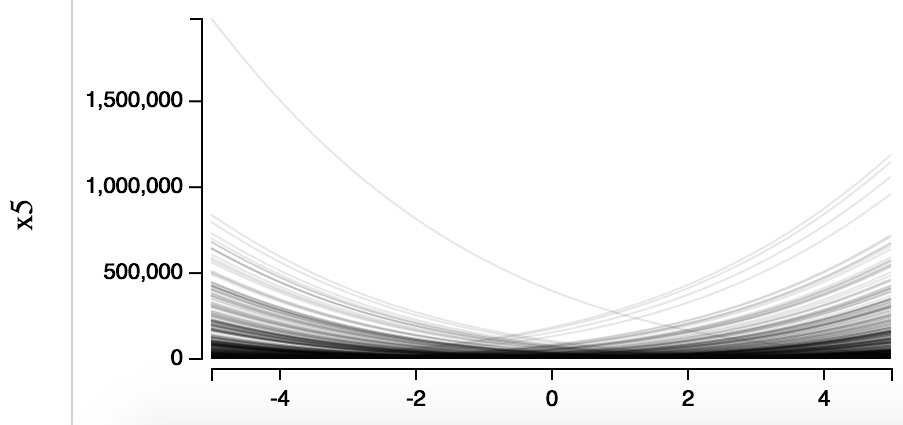
\includegraphics[width=\textwidth]{zakharov_confusing_unclustered.png}
    \caption{
    }
    \label{fig:cluster:none}
  \end{subfigure}
  ~
  \begin{subfigure}[b]{0.48\columnwidth}
    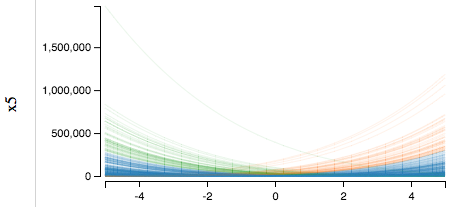
\includegraphics[width=\textwidth]{zakharov_color_clusters.png}
    \caption{
    }
    \label{fig:cluster:clustered}
  \end{subfigure}
  \caption{
    500 projected slices of the 5th dimension of the 5D Zakharov~\cite{Back:1996} 
    function. It is difficult to see if the slices are bowl shaped or two sets
    of monotonically decreasing and increasing curves. It is much clearer in 
    the cluster view that there are actually three sets of curves: 
    there is a set of monotonically decreasing curves and a set of 
    monotonically increasing curves. The very low-value curves form a third
    set.
  }
\end{figure}

Similar to visual encoding techniques such as parallel coordinate plots, projected 1D slices might mask certain patterns due to
overdrawing.
\autoref{fig:cluster:none} is an example where it is difficult to tell if the
slices are monotonic or bowl-shaped (\textbf{R-bowl}). The interactive slice highlighting
can give some insight into how individual slices are behaving but lacks
a global method to distinguish groups. We offer a
clustered slice view to address this (\autoref{fig:cluster:clustered}). 
The clustering is done with a k-nearest neighbor algorithm using the
$L^2$ distance between two slices as the distance metric.
This allows us to group the slices into distinct
groups of behavior and color-code these groups to distinguish them.

%These methods overcome many of the limitations of showing slices as
%compared to projection or topological methods while retaining the
%benefits. \msnote{hmmm ... coming back to my point from above: wouldn't it be good to first show that the general idea is good/better than STAR in certain cases before speaking of overcoming its limitations ... maybe this is just a framing issue ... }


\section{Task-based evaluation}
\label{sec:task-eval}

\definecolor{key0}{RGB}{242,240,247}
\definecolor{key1}{RGB}{203,201,226}
\definecolor{key2}{RGB}{158,154,200}
\definecolor{key3}{RGB}{106,81,163}
\newcommand\crule[1]{\textcolor{#1}{\rule{7pt}{7pt}}}

\begin{table*}[t]
  \centering
  \caption[Summary of the task-based evaluation]{%
    This table shows the summary of the task-based evaluation. I extended the discrete 
    data-focused tasks of Amar, Eagan, and Stasko~\cite{Amar:2005} to directly address
    continuous data, with the exception of ``sort'' (see \autoref{sec:task-eval}). 
    The table shows the scores from our qualitative results inspection as well as
    the expert study on a scale from
    ``none''~\crule{key0}, ``partially''~\crule{key1}, ``mostly''~\crule{key2},
    to ``fully''~\crule{key3}
    where
    ``none'' means that the task is not addressed at all and ``fully'' means 
    that this
    task is directly supported by this view. There are quotes of
    the general description from Amar, Eagan, and Stasko's paper in the ``discrete''
    column for reference. 
  }
  \label{tbl:task_list}
  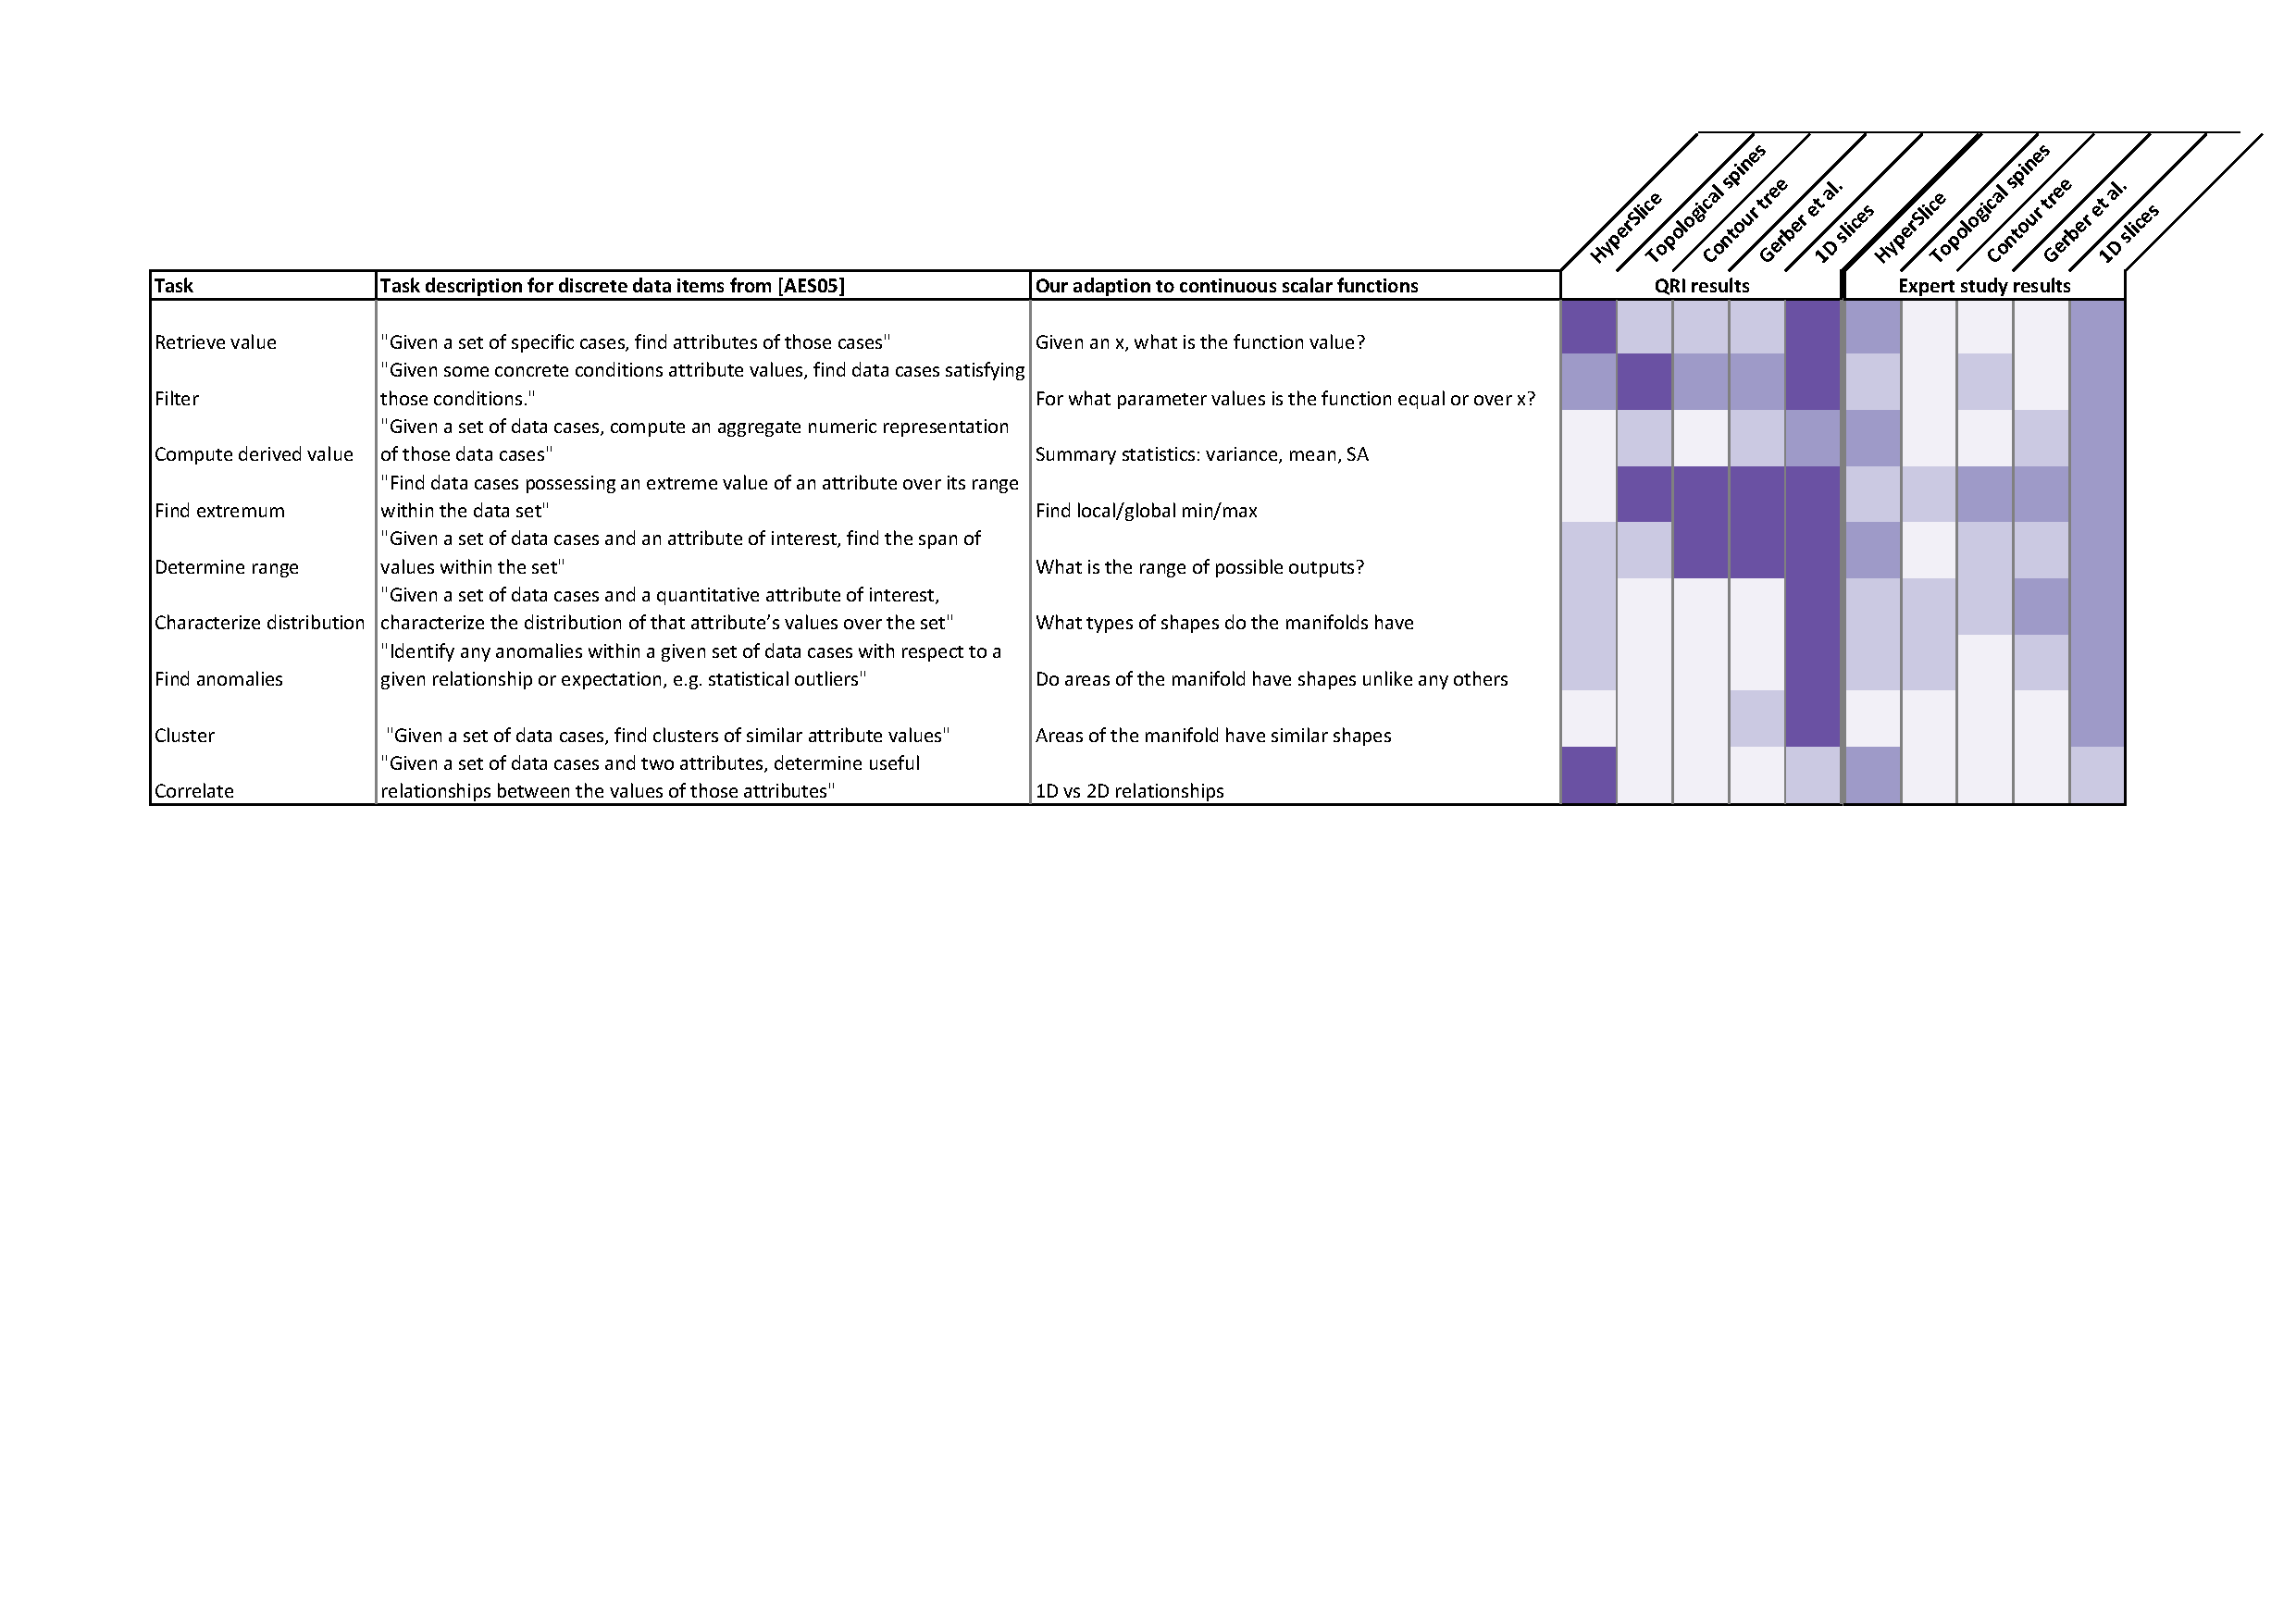
\includegraphics[width=\textwidth]{sp_task_list.pdf}
\end{table*}

\begin{figure}[tb]
  \centering
  \subcaptionbox{HyperSlice~\cite{Wijk:1993}\label{fig:compare:hs}}
    [0.48\textwidth]
    {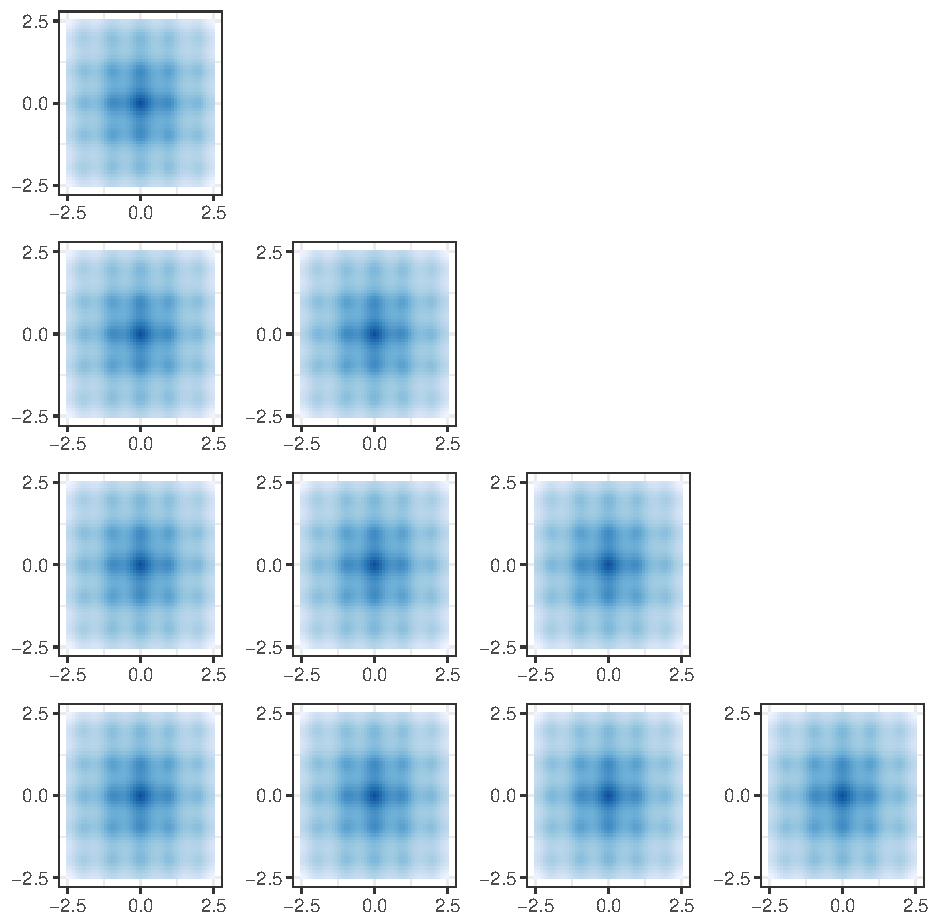
\includegraphics[width=0.17\textwidth]{ackley_5d_hs.pdf}}
  \hfill
  \subcaptionbox{Topological spine~\cite{Correa:2011}\label{fig:compare:ts}}
    [0.48\textwidth]
    {
\includegraphics[width=0.17\textwidth]{topo_spine.pdf}}
  \\
  \subcaptionbox{Contour tree~\cite{Carr:2003}\label{fig:compare:ct}}
    [0.48\textwidth]
    {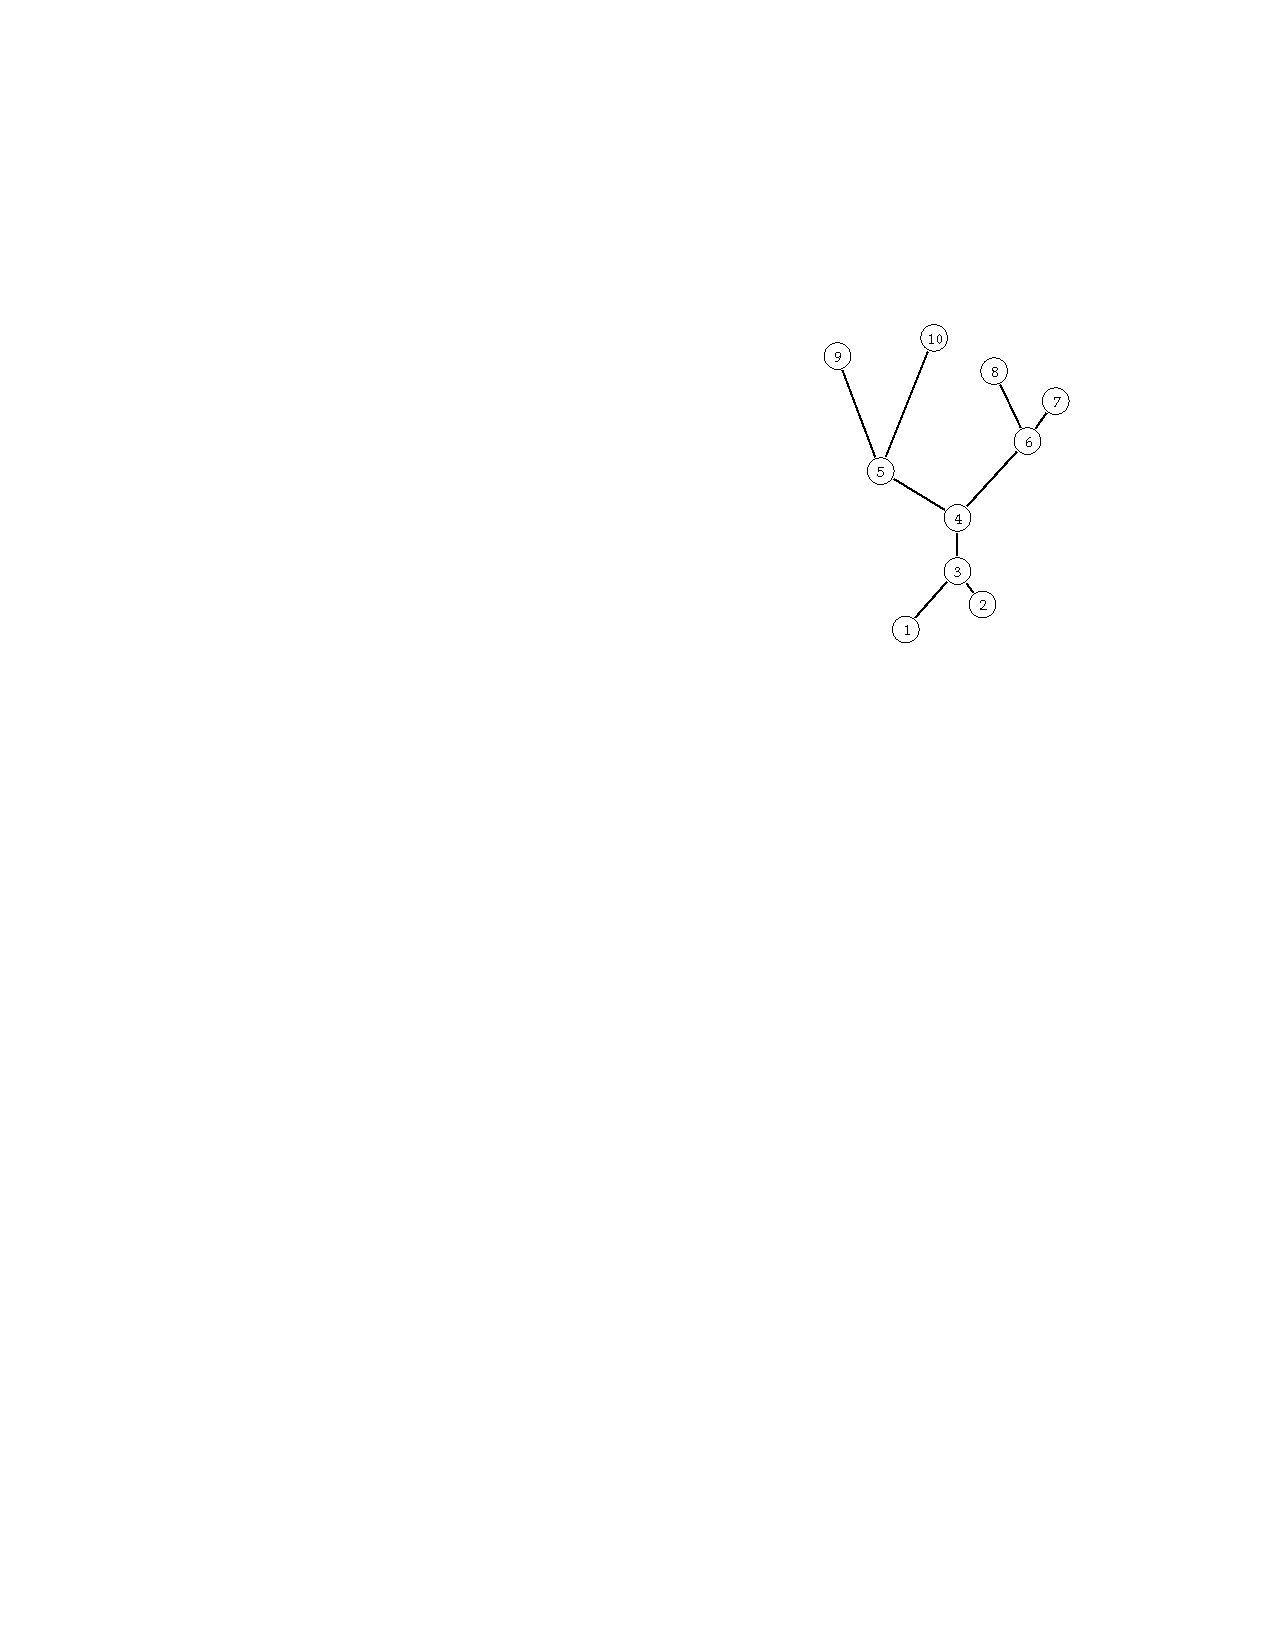
\includegraphics[width=0.17\textwidth]{contour_tree.pdf}}
  \hfill
  \subcaptionbox{Gerber et al.~\cite{Gerber:2010}\label{fig:compare:gerber}}
    [0.48\textwidth]
    {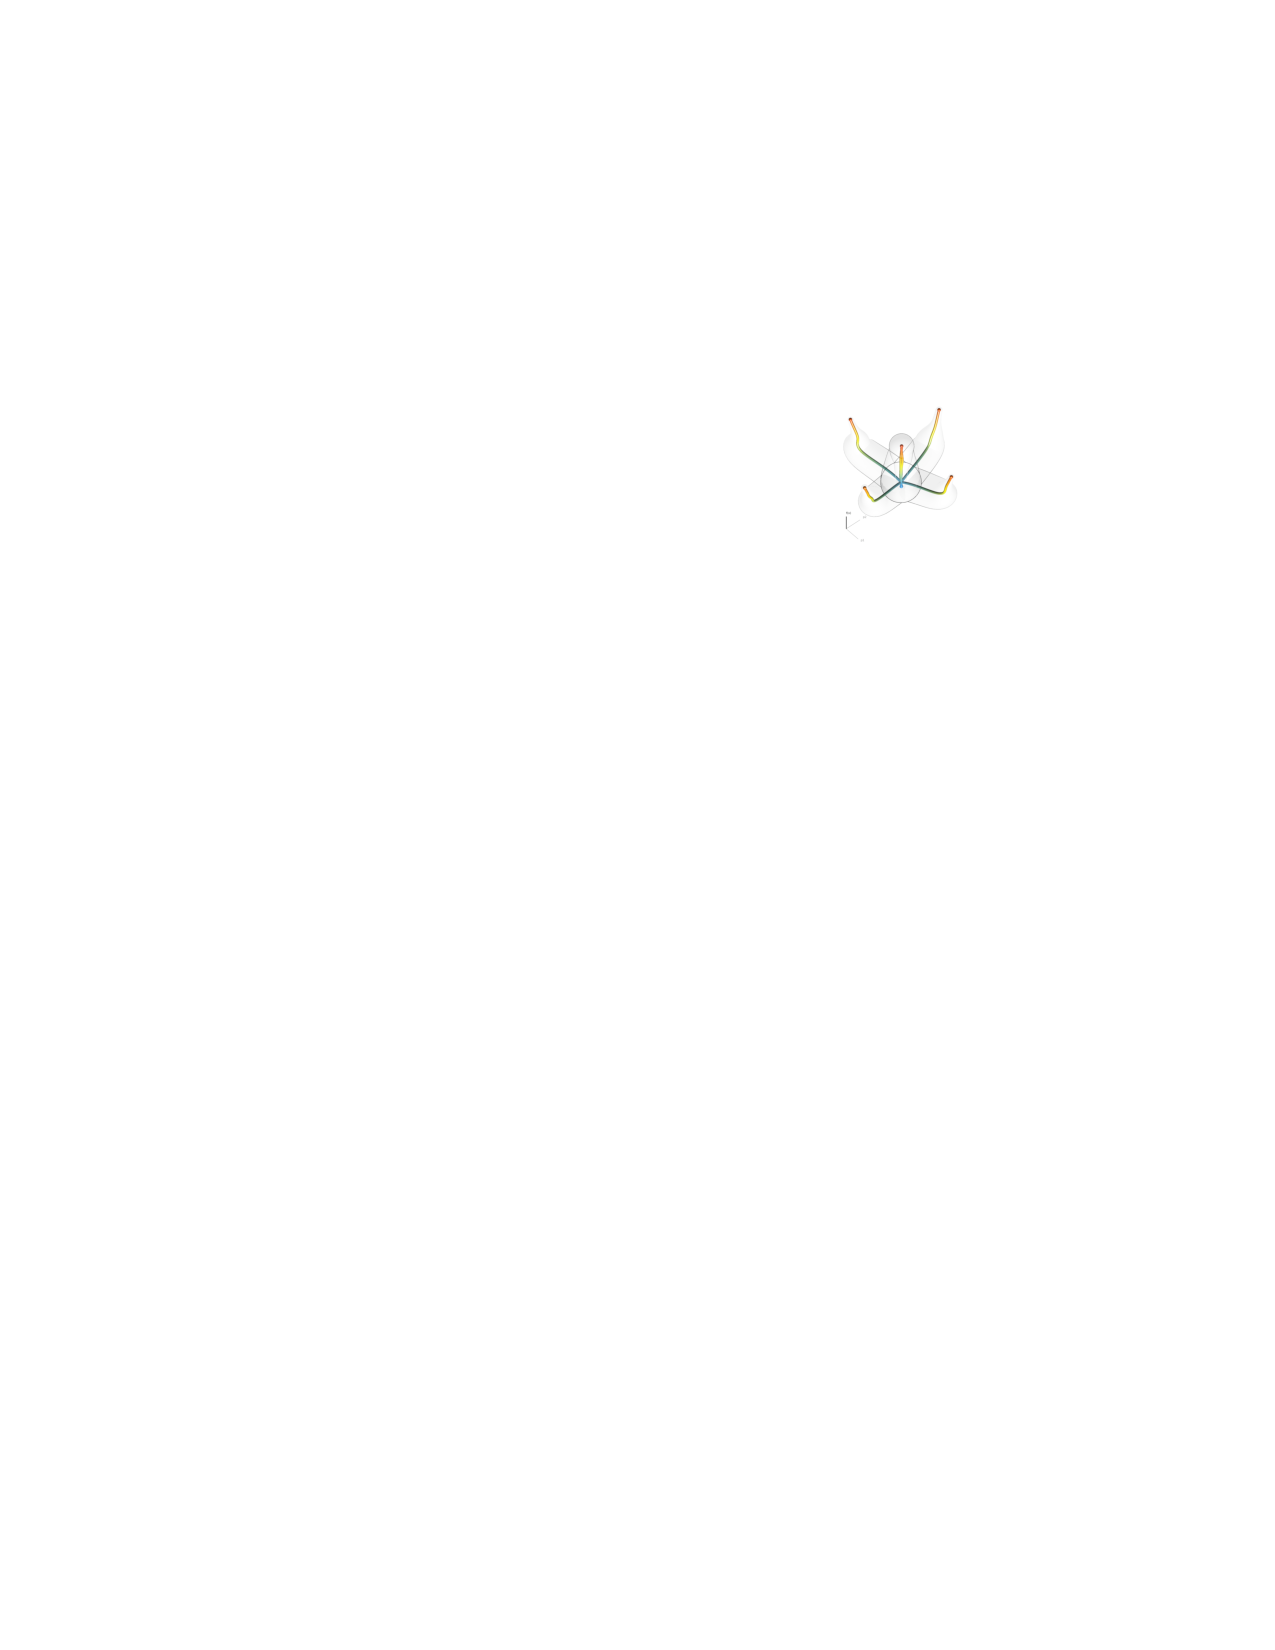
\includegraphics[width=0.17\textwidth]{gerber_ms.pdf}}
  %~
  %\subcaptionbox{1D slices\label{fig:compare:slices}}
    %[0.15\textwidth]
    %{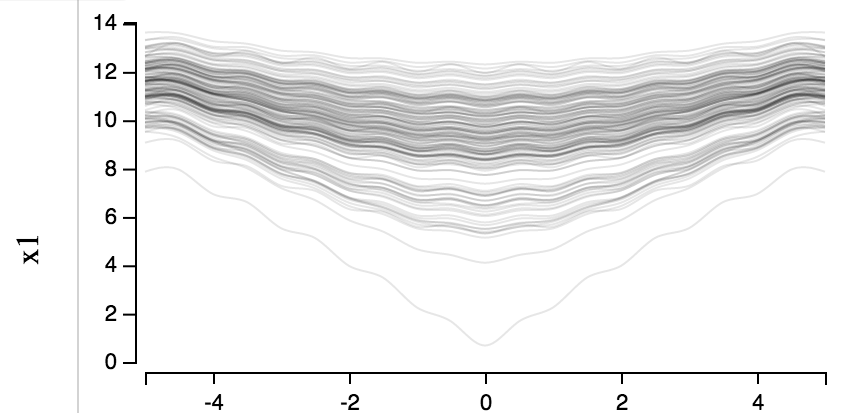
\includegraphics[width=0.1\textwidth]{images/4d_ackley_150slices.png}}
  \caption[The four techniques we used to compare with 1D slices.]{%
    The four techniques we used to compare with 1D slices. With
    the exception of HyperSlice, the images are from the respective papers and show different datasets used in their context.
  }
  \label{fig:compare}
\end{figure}

I first evaluate 1D slices in terms of their flexibility to deal with a broad
set of different low-level tasks.  Task taxonomies give a basis for comparing
visualization techniques to each other~\cite{Munzner:2014}.
If a technique addresses a large number of tasks, that is usually a good
indicator of its flexibility.  Over the last years, many different taxonomies
have been proposed~\cite{Amar:2005,Brehmer:2013,Heer:2012,Sedlmair:2014}.
However, to the best of my knowledge, none of these taxonomies thus far had a
dedicated focus on the visual analysis of multi-dimensional \textit{continuous}
data. I thus took a popular taxonomy for tasks on discrete data, by Amar,
Eagan, and Stasko~\cite{Amar:2005}, and extended each of their task categories
to directly address continuous data. This is an initial step towards
more consideration of multi-dimensional continuous data as a first class
citizen when developing task hierarchies.

Using this list of tasks, I compare 1D slices to other state of the art
techniques for multi-dimensional continuous data: HyperSlice~\cite{Wijk:1993},
topological spines~\cite{Correa:2011}, contour trees~\cite{Carr:2003}, and the
technique by Gerber et al.~\cite{Gerber:2010} (see \autoref{fig:compare}).  We
refer to topological spines, contour trees, and the work by Gerber et al.\ as
topological techniques when it makes sense to compare them as a group.
We evaluate based on all tasks, except for ``sort'', for which I could not
find a suitable extension to continuous functions.  The guiding theme in the
extensions is that users want to view the relationship of independent variables
to the dependent variable and to see how the dependent variable changes with
respect to the independent values.  The extensions are shown in
\autoref{tbl:task_list} along with the results of two investigations we
conducted based on them, as detailed in the following section.
\subsection{Study design}

To perform a task-based evaluation, I investigated the different techniques in two different ways.
First, I used a \textit{qualitative result inspection}
approach~\cite{Isenberg:2013}. 
I iteratively analyzed the techniques with different datasets and summarized
our discussion and analysis on a four point scale:
``None'' means that it is not possible to perform the task with the technique,
``partly'' means that it requires major interaction with the view to accomplish
the task, ``mostly'' means that one can accomplish the task with little
interaction, and ``fully'' means that this task is directly addressed by the
technique. 

Second, in order to get a more objective judgment I also asked 
\textit{four visualization experts} familiar with examining multi-dimensional spaces like
parameter space exploration to examine the eight datasets with different
techniques and rate how well each task can be accomplished with each technique
on the same scale. \autoref{fig:compare} shows the averaged results along with the
results of the qualitative result inspection in \autoref{fig:compare}.

For the techniques, I use my own implementation of HyperSlice and topological
spines since no code was available. I used the \texttt{msr} R
package~\cite{Gerber:2012} which implements the algorithm of Gerber et
al.~\cite{Gerber:2010}. For the contour tree I used the \texttt{libtourtre}
library and then rendered the trees using GraphViz using the
Sugiyama~\cite{Gansner:1993} layout.  As datasets, I chose the 2D sinc
function, 5D Rosenbrock~\cite{Rosenbrock:1960} function, 6D Ackley function, a
26 node hidden layer neural network built on the Boston housing
dataset~\cite{Lichman:2013}, a support vector machine with Gaussian kernel
built on the housing dataset, the fuel 3D volume dataset~\cite{Roettger:2017},
and the neghip 3D volume dataset~\cite{Roettger:2017}.  
Not all datasets could be rendered with all techniques due to software errors.

\subsection{Results}\label{sec:task-solutions}

In this section, I summarize our discussion about the strengths and weaknesses
of each technique in terms of performing the task.  For more details, there is
also a website that contains details of how each visualization technique can
solve each task. The website is available at
\url{http://sliceplorer.cs.univie.ac.at}.

%\msnote{TO-DISCUSS why is extending tasks from discrete to continuous domain a valid approach?}

\textbf{Retrieve value}:\label{retrieve-value}
In the discrete case, the user should be able to look at a point and get the
detailed values of it. In the continuous case we are interested in what the
function value is for a certain input parameter setting. All the techniques
support this although with the topological methods this is only possible for
the extrema and saddle points as all other points are filtered out. For
example, there could be many points between node $4$ and $5$ in the contour
tree (\autoref{fig:compare:ct}). With
slicing techniques, both 1D and 2D, the values can be read directly off the
chart. Of course, for all techniques the adding of interaction, such as a tooltip, can make retrieving concrete values even easier. 

\textbf{Filter}:\label{filter}
Amar, Eagan, and Stasko describe this task as a general filtering query on data points.
In the continuous case, the user wants to understand the outputs of the
function. This is a query as to where the function value is in a certain range.
With continuous data this is the domain of isosurface extraction.
This is possible with slicing techniques by visual examination.
With HyperSlice, though, one must be careful to view sufficient focus points to
get a general idea of where the function equals certain values.  Topological
spines also shows this directly and they use concentric areas 
(\autoref{fig:compare:ts}) to give a
general idea of the area that a particular value range takes up. The other
topological techniques allow one to see if a certain value is possible, for
example, we can see that the function represented by the contour tree in 
\autoref{fig:compare:ct} takes the values greater than 4 somewhere by seeing 
that there are edges from node 4 to nodes 5 and 6. However,
there is no relation back to the parameter settings that will produce these
values. 

\textbf{Compute derived value}:\label{compute-derived-value}
The direct interpretation of this task to continuous data is to compute derived
value results about the curves 
%\msnote{TO-DISCUSS: the curves? all 1D ones for one dimension? What about derived values that summarize the entire function?} 
like mean and variance. Many of these values can
also be perceived visually.  Topological methods compute the persistence value
between the function to determine what to show but with the exception of
topological spines this is hidden from the user. Topoplogical spines show a
graph of the persistence and ``saturated persistence'' which allows the user
to select which nodes to filter.
Projections of 1D curves allows us to see the distribution.
In
\autoref{fig:walkthrough}c we can see that there are very few function values
around the global minimum and the function has two types of behavior: a
periodic sine wave across the domain and a general parabola shape.

\textbf{Find extremum}:\label{find-extremum}
All the topological techniques we evaluated support this in some
way. With HyperSlice one needs substantial guidance on setting the focus point to find
extrema (like a histogram of function outputs). % or a gradient widget.  Since
1D slices is a global technique showing all slices at once, one can find
extrema by inspecting the graphs.
% see this
%directly since the slices are projected. Extreme values can be seen visually.
As previously mentioned, topological methods are purpose built to extract
extrema from continuous data. For example, it is easy to see that the function
using the method by Gerber et al.\ (\autoref{fig:compare:gerber}) has five
maxima and the function of the contour tree (\autoref{fig:compare:ct}) has four
maxima.

\textbf{Determine range}:\label{determine-range}
Amar, Eagan, and Stasko describe this as finding the range of possible values
for a particular attribute. There is really only one attribute of interest: the
values of the multi-dimensional scalar function. Any view from which we can
read the global minimum or the global maximum allows us to do this. Contour
trees, Gerber et al., and 1D slices all allow us to read these off the view.
Topological spines either show the global maximum \emph{or} the global minimum,
but not both.  HyperSlice has no way to do this directly by adjusting the focus
point.  However, one expert noticed that they could simply read the range of
the function off of the color legend.

\textbf{Characterize Distribution}:
\label{characterize-distribution}
Here again there is one key value of interest that we want to characterize: the
function value.  This requires a global view.  Projections of slices directly
show how the function slices are distributed.  We can see in
\autoref{fig:walkthrough}d that there are very few function values around the
global minimum but many around high values. It would be difficult to use
HyperSlice to truly understand the distribution of values. The user would
somehow have to browse around the focus points and then memorize the function
values. Topology throws away the spatial element and just shows the
relationships between extrema and saddles.

\textbf{Find anomalies}:\label{find-anomalies}
%\msnote{TO-DISCUSS what does an outlier mean in continuous lands? Is it really about shapes? Or is it about spiky-ish behavior?}
Anomalies in the discrete case are single point outliers. While that is also
possible in the continuous case, we may also have entire parts of the function
that are unlike any other part. These should also be identified.
In a global view like projected 1D slices these will show up visually. The
slices will stand out from the rest similar to other projection-based
techniques like scatterplots. With HyperSlice we must browse around until we
can see one directly. However, we will see it if we can find it. Topological
methods will only show extrema in terms of maxima or minima values but not
shape and hence mask anomalies and outliers.

\textbf{Cluster}:\label{cluster}
Since we are looking at manifold behaviors, we want to be able to group the
functions into areas of similar behavior. For example, are they monotonically
increasing or decreasing? Furthermore, can we find areas where the variance
changes? The topological technique of Gerber et al.~\cite{Gerber:2010} was
created to address just this. They split the function
into areas of monotonic behavior and then show a line indicating how those
monotonic regions are related to each other. However, the way they
reconstruct the function between extrema and saddle points does not allow us to
view the variance between these points as the 1D slice view
allows. Clustering the 1D slices tries to split the slices into groups of
similar behavior (see \autoref{fig:cluster:clustered}).

%\begin{figure}
  %\centering
  %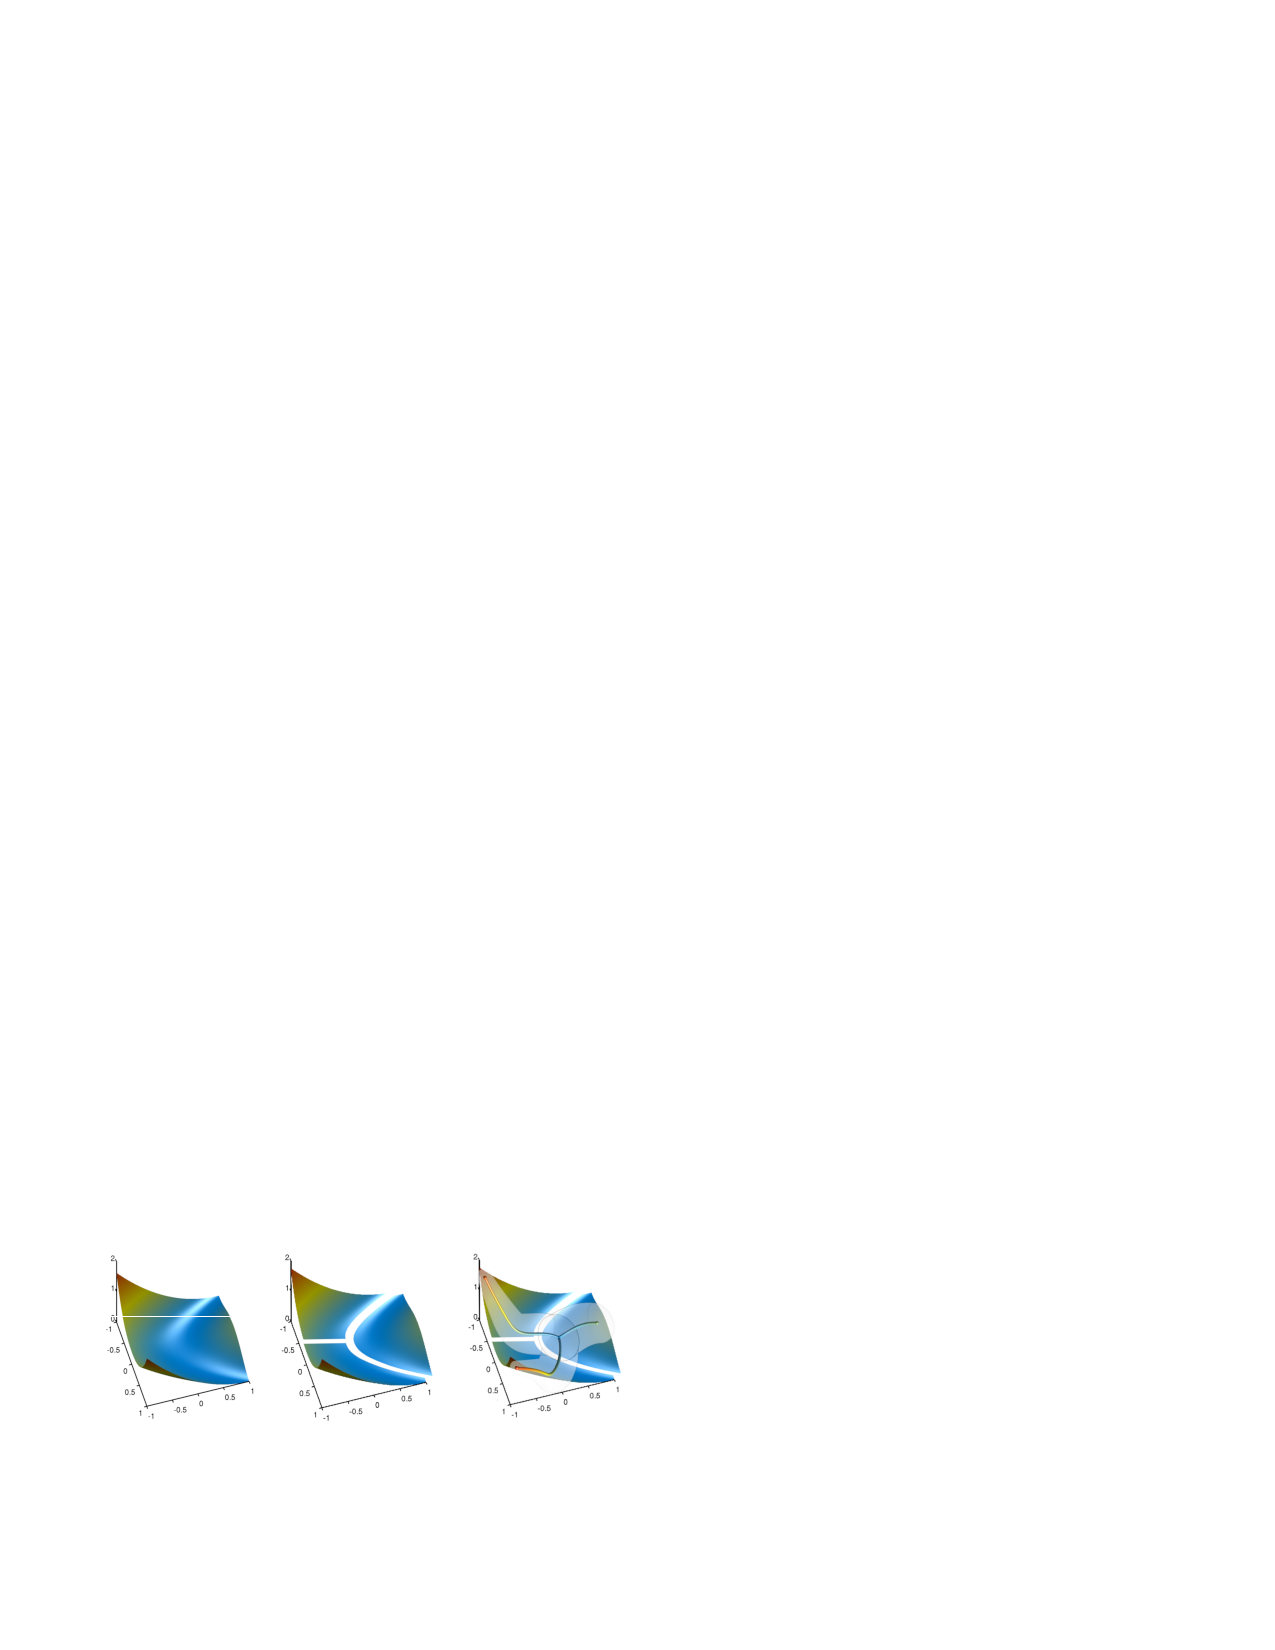
\includegraphics[width=\columnwidth]{images/gerber_evolution.pdf}
  %\caption{
    %How the method of Gerber et al.\ visualizes a function. They take a 
    %function (left image), decompose it into areas of monotonic behavior 
    %(center image), approximate each region with a regression model (right
    %image), and then show this regression model to the user.
    %(image from \cite{Gerber:2010}).
  %}
  %\label{fig:gerber}
%\end{figure}

\textbf{Correlate}:\label{correlate}
Finally, we consider correlation. In the discrete data case the goal is to find
correlation between attributes. With continuous data, we already have a
dependency between the independent and dependent variables. What we would like
to learn is how many variables have an influence on the function. With 2D views
(that only HyperSlice provides) one can see both 1D and 2D interactions with
the function. We can see that the function in \autoref{fig:compare:hs} has
radial behavior so the function value depends on both 1D and 2D interactions.
None of the other techniques are capable of showing 2D interactions between
parameters.

\subsection{Summary}

From the summary in \autoref{tbl:task_list} we can see that the 1D slices
technique addresses more of the tasks than any other technique.  It is not
always the highest performing view though.  HyperSlice is the only technique 
evaluated that could show more than one-dimensional interactions but it does
not do well on global tasks like extrema detection. The various topological
techniques directly address tasks related to extrema detection and comparison
but do not perform as well on others. 
%\ttwnote{should the following go in limitations?}
The experts often commented that they felt they needed more knowledge about
what exactly the topological techniques were doing in order to interpret
the results. Thus, the ratings for these techniques may be artificially low.
%\ttwnote{However, given the difficulty that experts had with the technique,
%this does not bode well for the general public.}
I conclude that 1D slices are a
very flexible technique indeed.  



\section{Usage scenarios}\label{sec:usage-scenarios}

In addition to evaluating 1D slices with a low-level task hierarchy, we also
provide usage scenarios to understand their value in real-world applications.
We begin with an illustrative example using the 2D sinc
function.
%\ttwnote{cite?}.  TM: No need to cite!
We then use our 1D slices approach to illustrate how
it can help better understand neural network architectures for a regression
problem. Finally, we use 1D slices to investigate the effect of initial
position on optimization algorithm performance.

The purpose of these evaluations is a proof of concept that 1D slices can be
used for real-world problems. In particular, it is not meant as a comparative
evaluation as provided in the previous section. To the best of our knowledge,
neither HyperSlices nor topological techniques have been applied to
understanding neural networks nor optimization algorithms so far. A full
adaption of, and comparison to, these techniques for the provided use cases are
beyond the scope of this paper, and are left for future work. 

\subsection{2D sinc function}

\begin{figure}
  \centering
  \begin{subfigure}[b]{0.3\linewidth}
    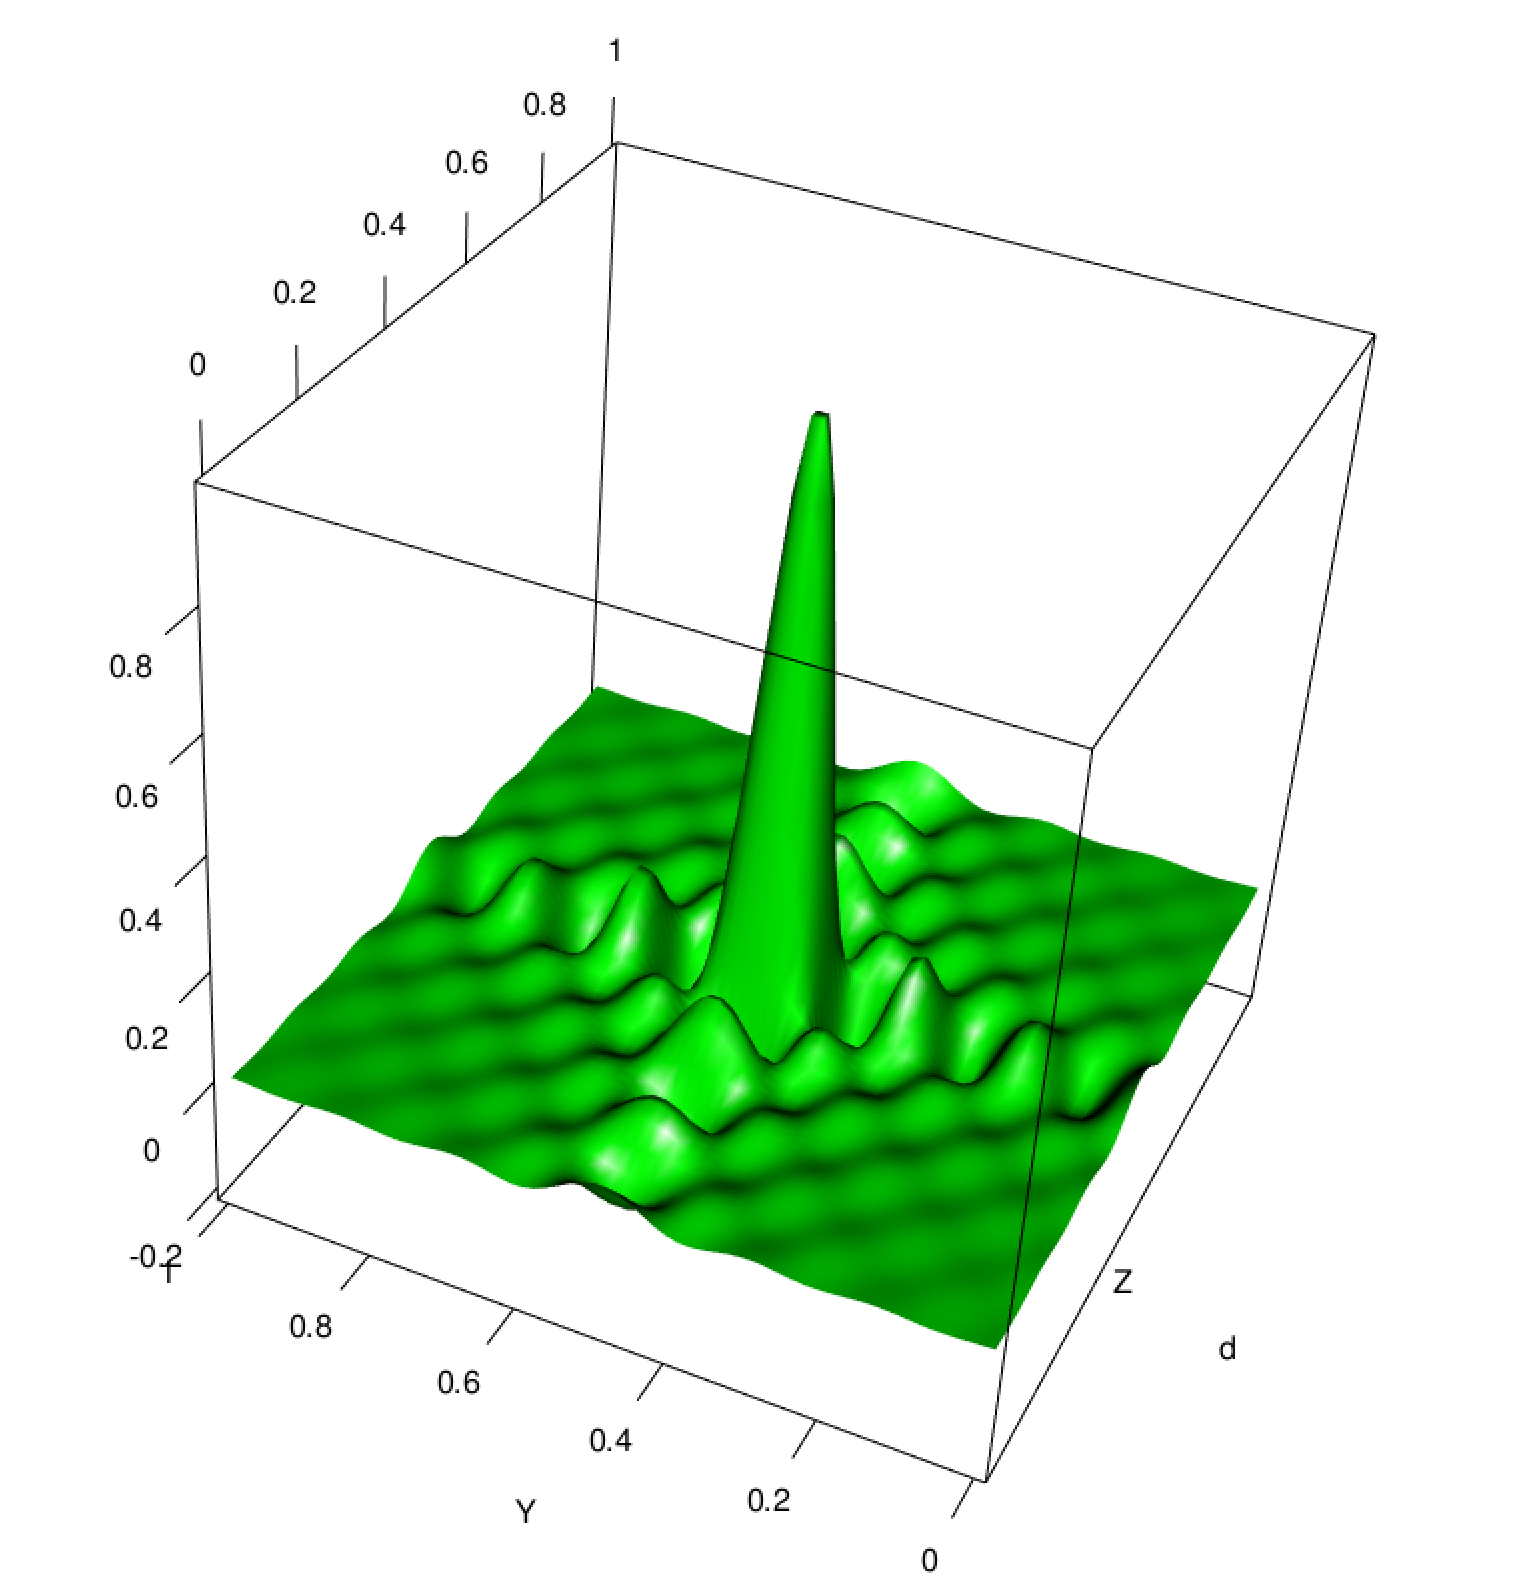
\includegraphics[width=\textwidth]{sinc_3d.png}
    \caption{
      Surface plot
    }
    \label{fig:sinc:3d}
  \end{subfigure}
  \qquad\qquad%
  \begin{subfigure}[b]{0.3\linewidth}
    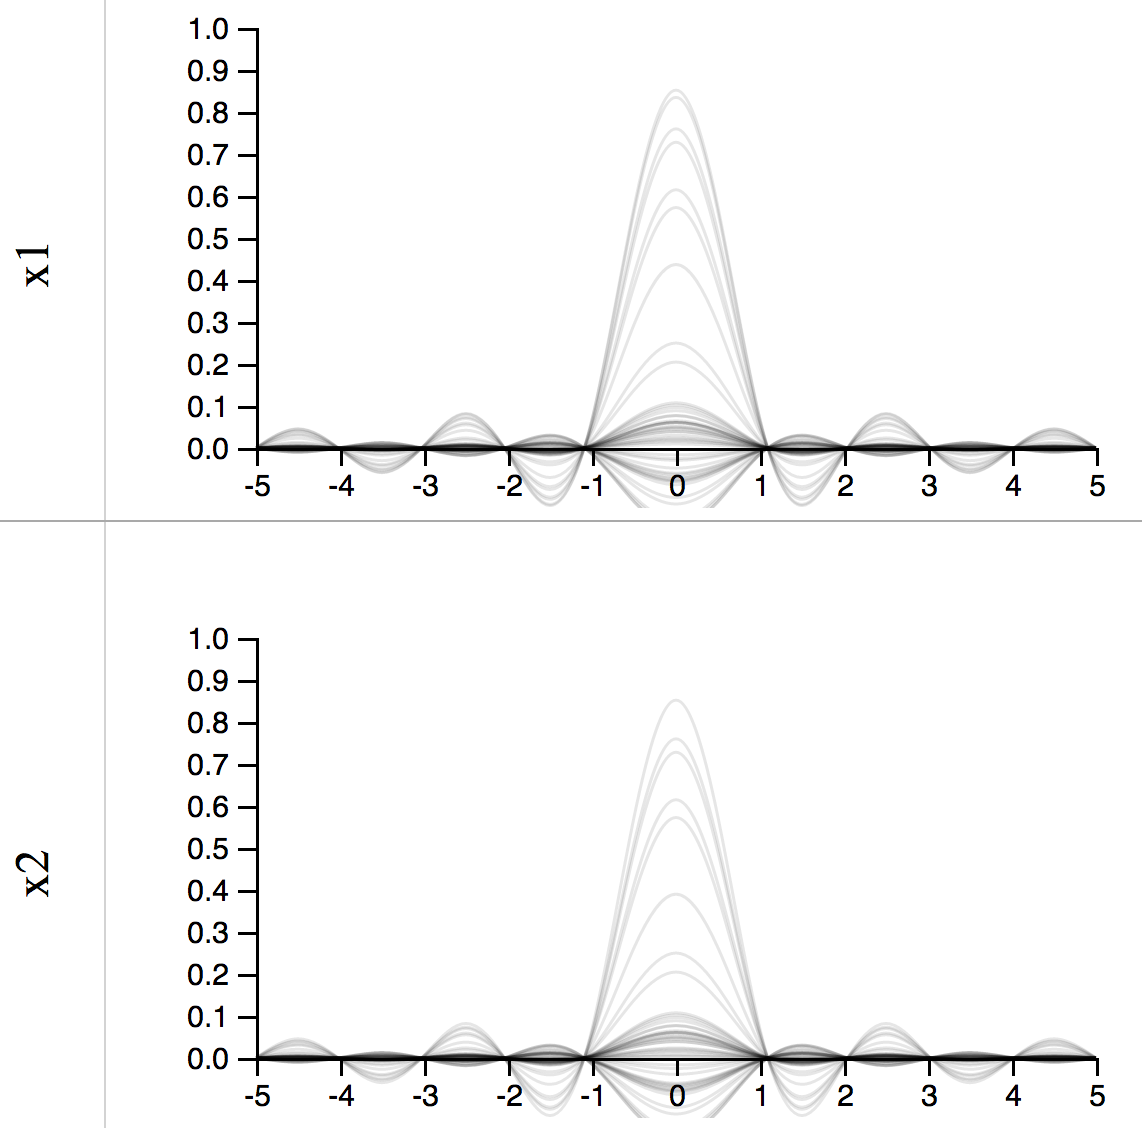
\includegraphics[width=\textwidth]{sinc_sp.png}
    \caption{
      1D slices
    }
    \label{fig:sinc:sp}
  \end{subfigure}
  \\
  \begin{subfigure}[b]{0.3\linewidth}
    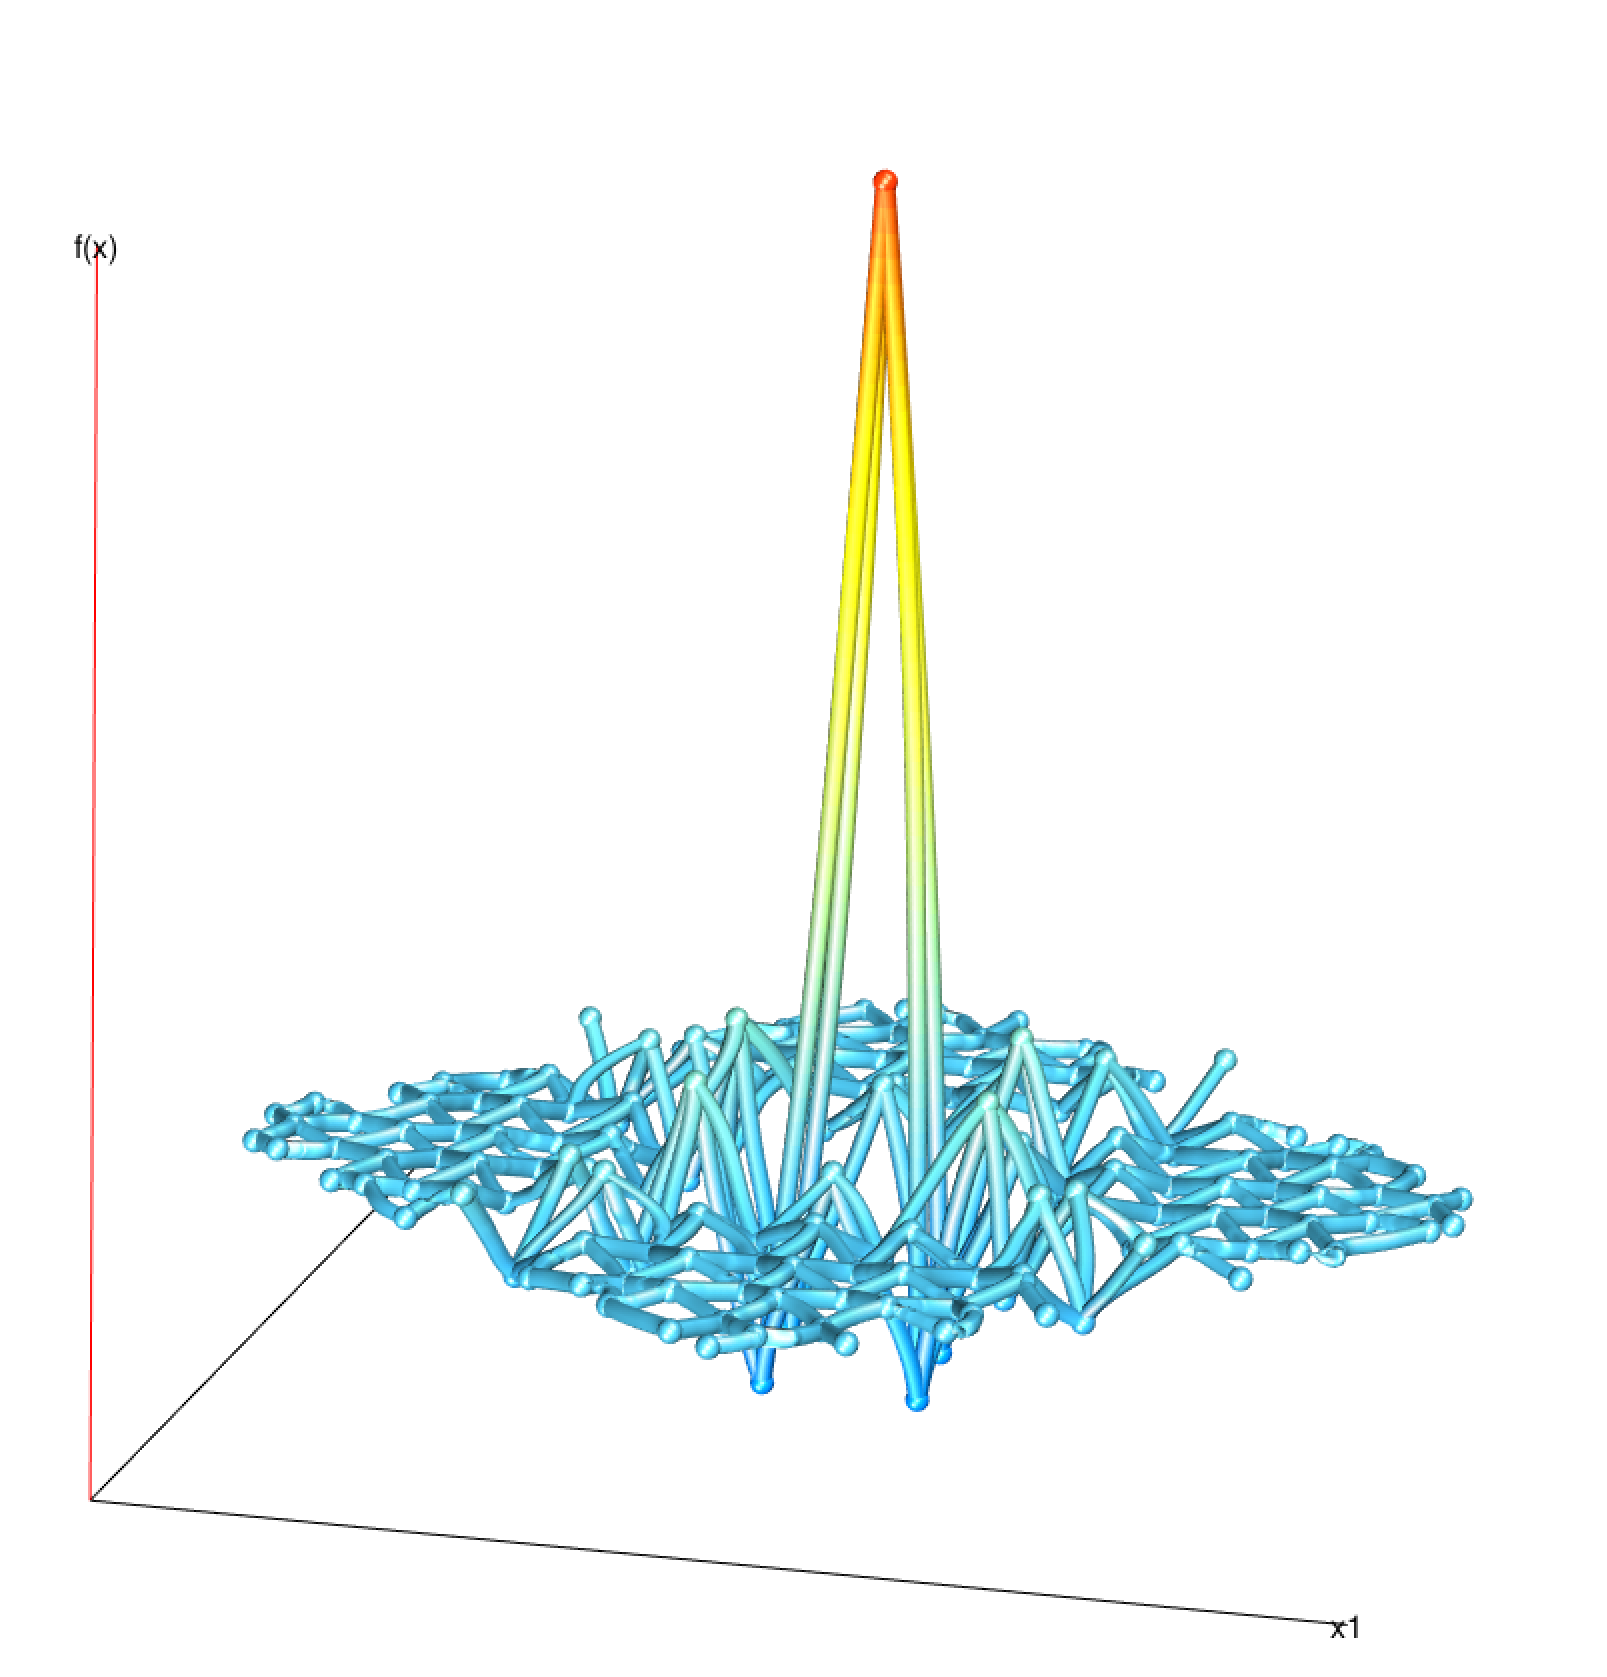
\includegraphics[width=\textwidth]{sinc_ms_1.png}
    \caption{
      $\texttt{pLevel} = 0.0$
    }
    \label{fig:sinc:ms_1}
  \end{subfigure}
  \hfill
  \begin{subfigure}[b]{0.3\linewidth}
    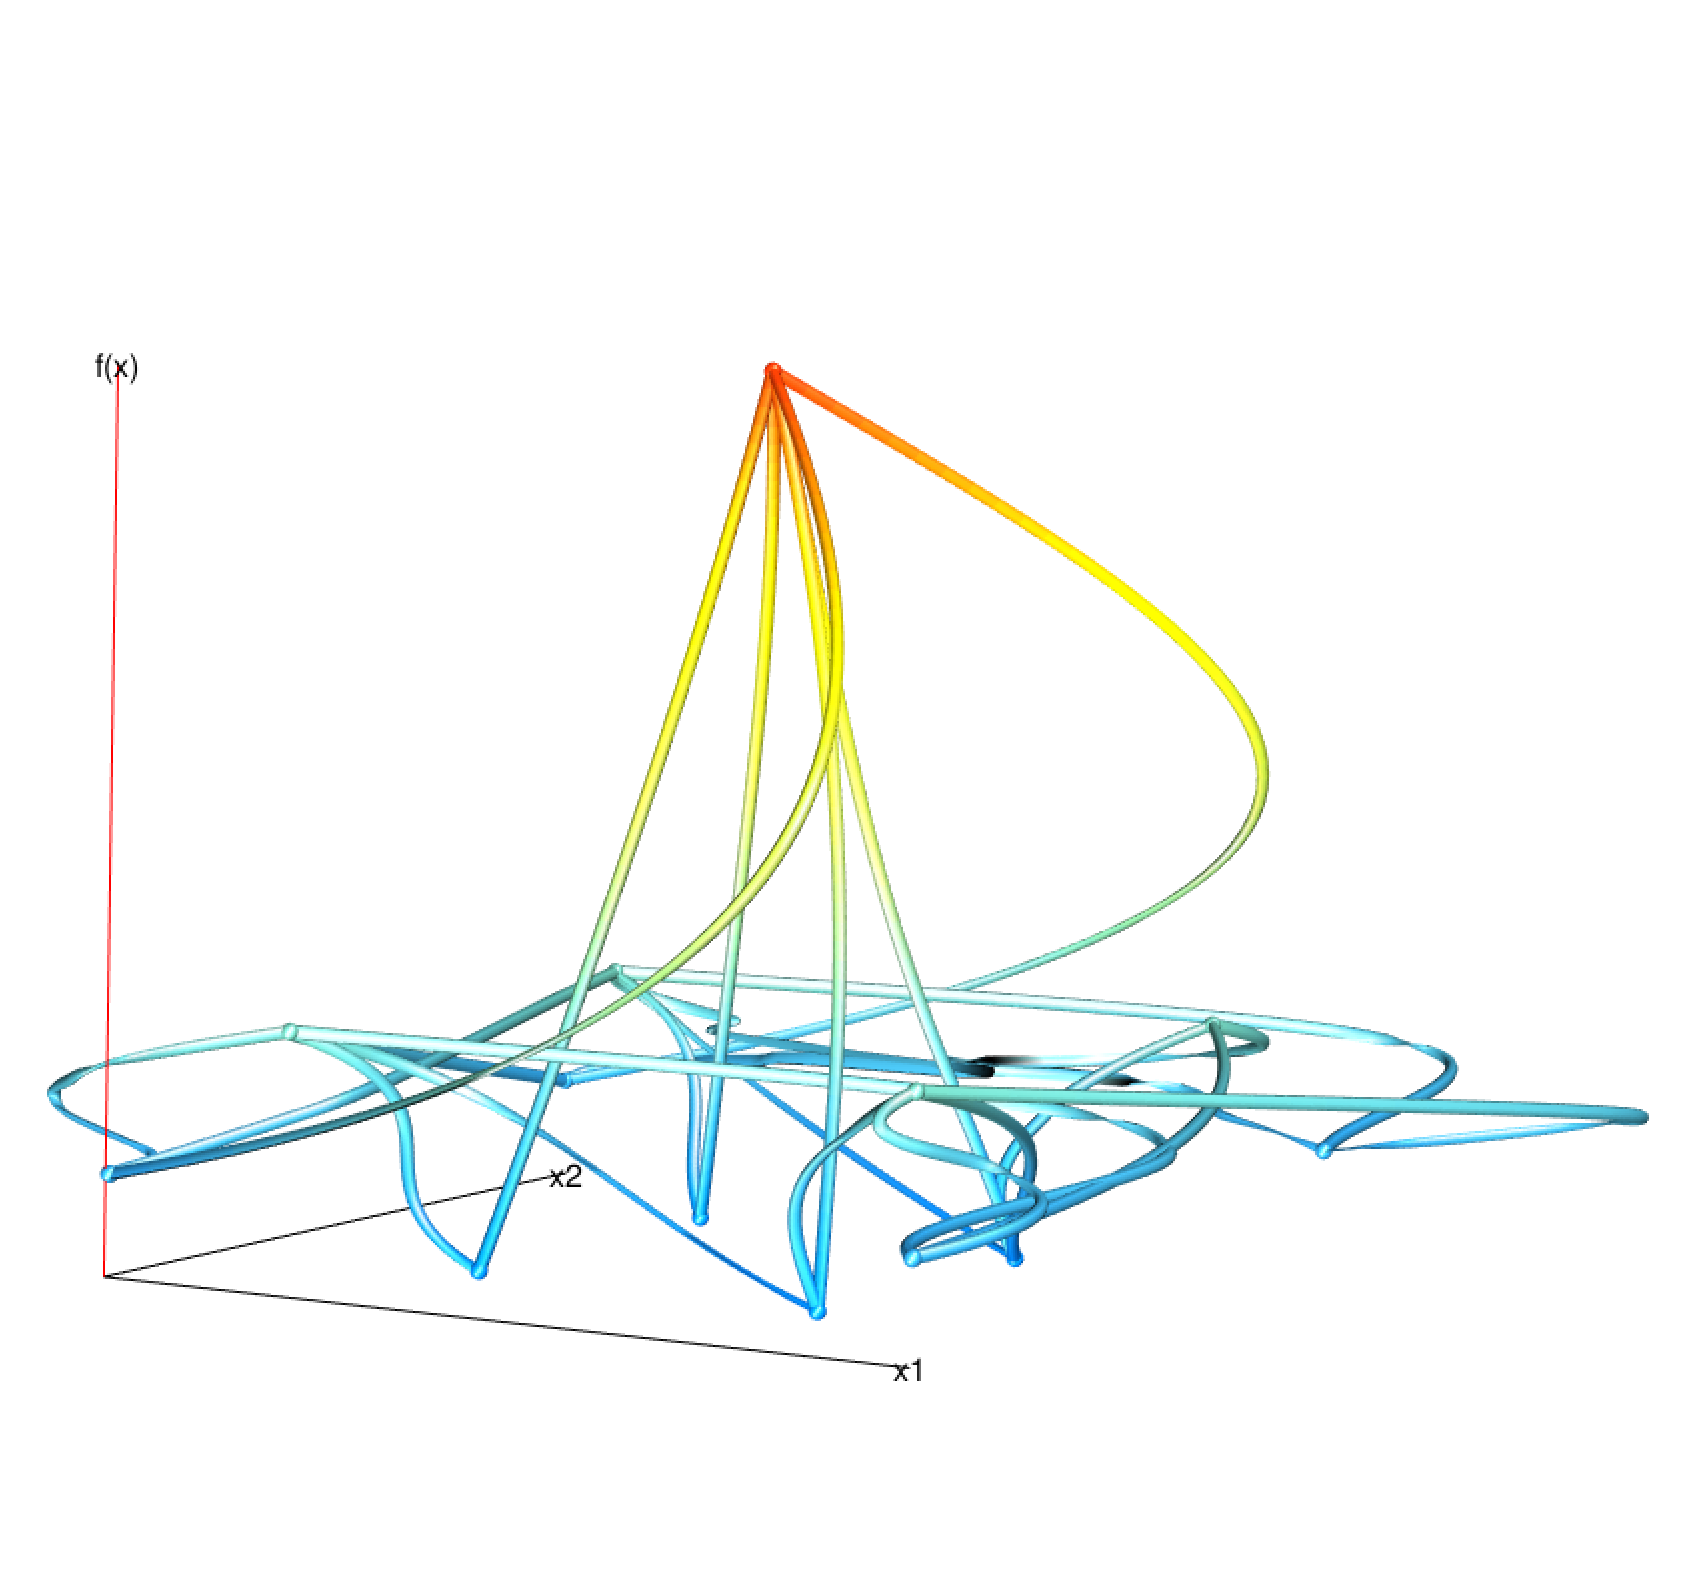
\includegraphics[width=\textwidth]{sinc_ms_2.png}
    \caption{
      $\texttt{pLevel} = 0.05$
    }
    \label{fig:sinc:ms_2}
  \end{subfigure}
  \hfill
  \begin{subfigure}[b]{0.3\linewidth}
    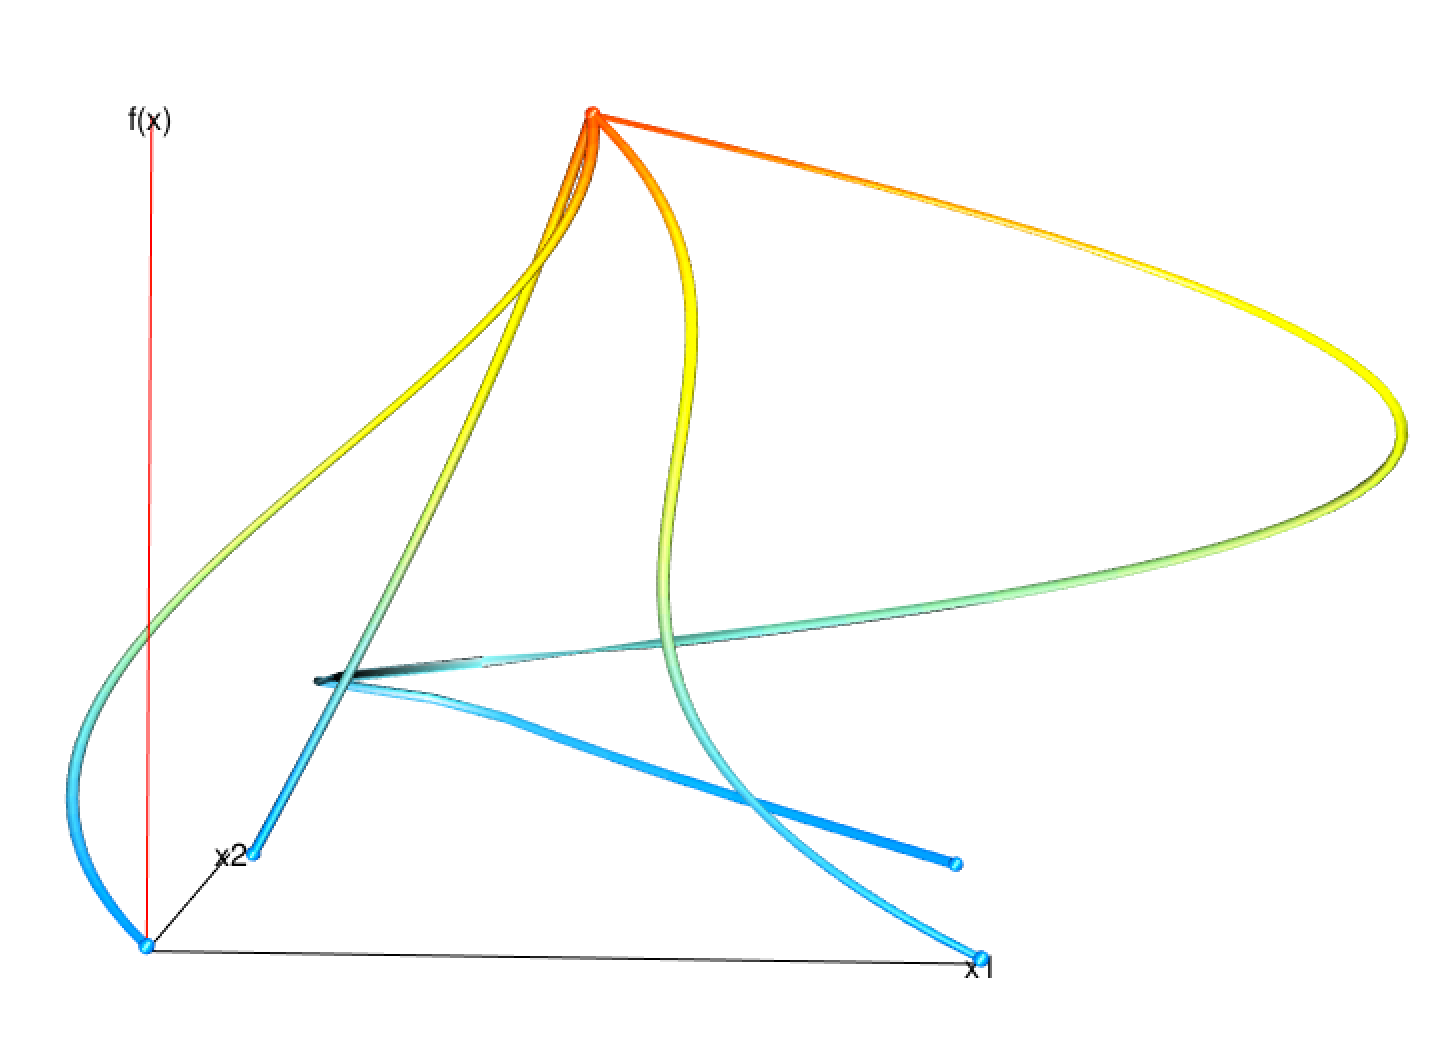
\includegraphics[width=\textwidth]{sinc_ms_3.png}
    \caption{
      $\texttt{pLevel} = 0.1$
    }
    \label{fig:sinc:ms_3}
  \end{subfigure}
  \caption{
    Different views of the 2D sinc function. We show the surface plot
    in (\subref{fig:sinc:3d}) for reference. Our 1D slice view is shown
    in (\subref{fig:sinc:sp}). The central peak as well as the sub peaks
    are prominent. For comparison we show the method of Gerber et 
    al.~\cite{Gerber:2010} in 
    (\subref{fig:sinc:ms_1})--(\subref{fig:sinc:ms_3}) at different levels 
    of persistence filtering. 
    With no filtering (\subref{fig:sinc:ms_1}) the graph looks much like the
    original function. The plot is very sensitive to the filtering level.
    (\subref{fig:sinc:ms_2}) and (\subref{fig:sinc:ms_3}) are all very 
    different from each other.
  }
  \label{fig:sinc}
\end{figure}

Imagining how a function in more than 3-dimensions looks is difficult if not
impossible. In order to illustrate how Sliceplorer visualizes functions we show
the 2D sinc function. 
%\tmnote{The sinc function is a the perfect reconstruction function in the band limited case.}
We are using the formulation where 
$y(x_1,x_2) = \frac{sin(\pi x_1)}{\pi x_1} \frac{sin(\pi x_2)}{\pi x_2}$.
In \autoref{fig:sinc:3d} we show a 3D surface plot of this function. The 
global maximum is at $x_1,x_2 = 0,0$ where $y=1$. There are a number of local
maxima and minima of decreasing value radiating out from the origin.

We show the 1D slice view using Sliceplorer in \autoref{fig:sinc:sp}.
We are showing 50 slices in each of the 2 plots. We can clearly see that
the maximum value occurs when $x_1,x_2 = 0,0$ in the graph at around $y=1$.
We can also see the decreasing extrema radiating out from the origin. We can
also precisely measure the height and x-location of the extrema. If we want
to examine a particular trace then we can highlight it in the view and see
the full slice highlighted on screen.

For comparison, we show visualizations of the 2D sinc function rendered using
the \texttt{msr} package~\cite{Gerber:2012} in R. This package implements the
visualization of the Morse-Smale complex from Gerber et al.~\cite{Gerber:2010}.
We sampled the function with $2000$ sample points using a Sobol sequence. The
1D slices view is showing $50$ focus points with $21$ samples for each slice so
this was done to use a similar sampling method and number of samples to the
Sliceplorer method. The function can do persistence-based filtering of the
graph before rendering.  This is controlled by the \texttt{pLevel} parameter
which filters all persistences less than a certain value. In
\autoref{fig:sinc:ms_1} we show the view with the filtering level set to $0$,
i.e.\ no filtering. The view does a very good job showing the critical points
of the graph. It looks very similar to the surface plot
(\autoref{fig:sinc:3d}). However, the visualization is very sensitive to the
filtering level. In \autoref{fig:sinc:ms_2} and \autoref{fig:sinc:ms_3} we show
the sinc function with the filtering level set to $0.05$ and $0.1$
respectively.  The 1D slice view does not suffer from this issue of
parameterization.

\subsection{Neural networks}\label{neural-networks}

\begin{figure*}[t]
  \centering
  \begin{tabular}[b]{cccc}
    Neural network - 26 & SVM - polynomial & Neural network 5+3 & SVM - radial \\
    \hline \\
    \begin{subfigure}[b]{0.2\textwidth}
      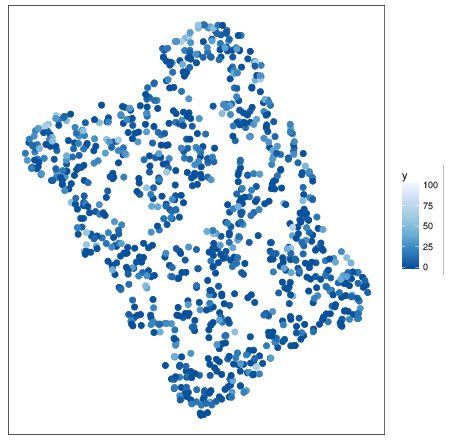
\includegraphics[width=\textwidth]{boston_nn_26_sp.png}
      \caption{
      }
      \label{fig:nn_comp:a}
    \end{subfigure}
    &
    \begin{subfigure}[b]{0.2\textwidth}
      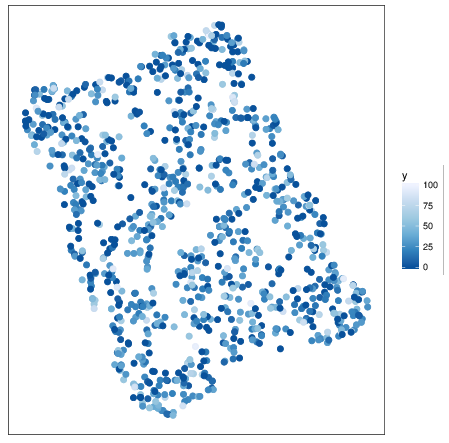
\includegraphics[width=\textwidth]{boston_svm_poly_sp.png}
      \caption{
      }
      \label{fig:nn_comp:b}
    \end{subfigure}
    &
    \begin{subfigure}[b]{0.2\textwidth}
      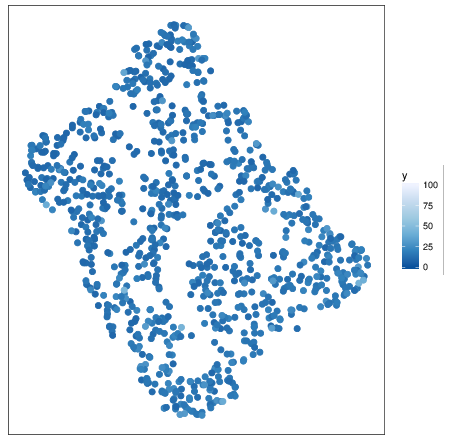
\includegraphics[width=\textwidth]{boston_nn_5x3_sp.png}
      \caption{
      }
      \label{fig:nn_comp:c}
    \end{subfigure}
    &
    \begin{subfigure}[b]{0.2\textwidth}
      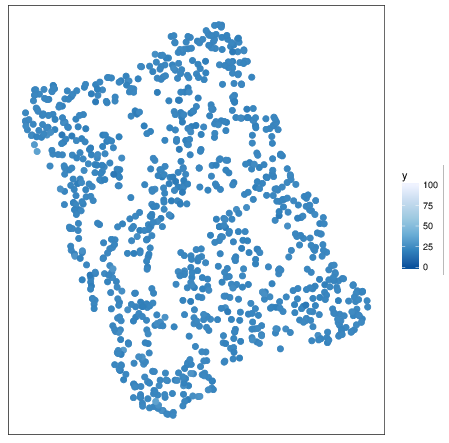
\includegraphics[width=\textwidth]{boston_svm_radial_sp.png}
      \caption{
      }
      \label{fig:nn_comp:d}
    \end{subfigure} \\
    \begin{subfigure}[b]{0.2\textwidth}
      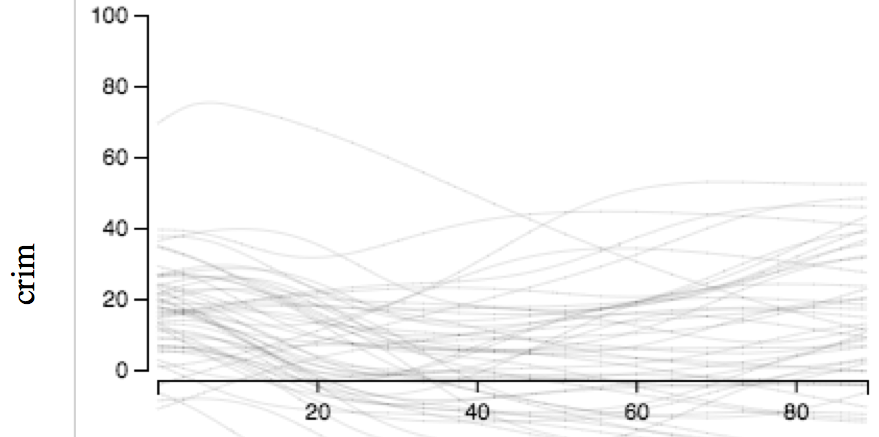
\includegraphics[width=\textwidth]{boston_nn_26_slices.png}
      \caption{
      }
      \label{fig:nn_slices:e}
    \end{subfigure}
    &
    \begin{subfigure}[b]{0.2\textwidth}
      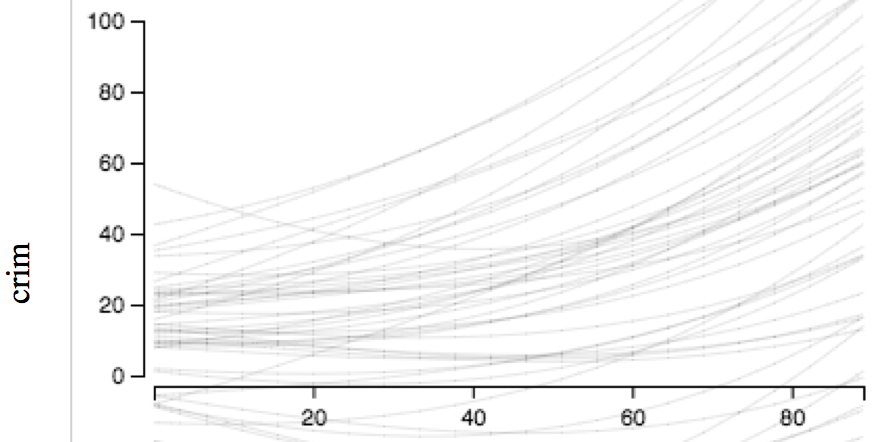
\includegraphics[width=\textwidth]{boston_svm_poly_slices.png}
      \caption{
      }
      \label{fig:nn_slices:f}
    \end{subfigure}
    &
    \begin{subfigure}[b]{0.2\textwidth}
      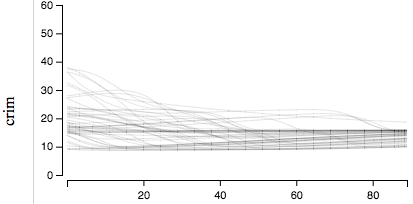
\includegraphics[width=\textwidth]{boston_nn_5x3_slices_zoomed.png}
      \caption{
      }
      \label{fig:nn_slices:g}
    \end{subfigure}
    &
    \begin{subfigure}[b]{0.2\textwidth}
      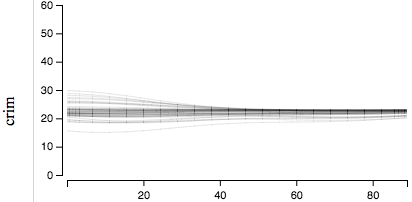
\includegraphics[width=\textwidth]{boston_svm_radial_slices_zoomed.png}
      \caption{
      }
      \label{fig:nn_slices:h}
    \end{subfigure}
  \end{tabular}
  \caption{
    Two different views of the predictions of four different machine learning
    regression models on the Boston housing dataset. The top row (a -- d) shows
    predictions by each model compressed to two dimensions with t-SNE. We
    colored the points on a continuous color scale with dark blue being 0 and
    light blue the highest value. The bottom row (e -- h) shows a 1D slice view
    of the first dimension of the dataset, crime rate. We show the slices of
    the remaining dimensions in the supplemental material. 
    The 1D slices reveal interesting information about how the models perform and
    can assist with model selection. We may not want to use the SVM with
    polynomial kernel (f), for example, since it predicts that home price will go
    up with higher crime rates.
  }
  \label{fig:nn_comp}
\end{figure*}

%\msnote{sounds a bit too defensive. Deep Learning is the big hype at the moment but nobody understands them! That's imho the core message that we need to say}
Artificial neural networks are currently gaining a lot of attention in machine
learning.  The goal of these algorithms is to produce a multi-dimensional
function fitted to the training points. Neural networks, in particular, have
proven to be very good at producing accurate, generalizable predictions. One of
the major challenges for designers of such models, however, is to properly
architect these networks. For instance, how many hidden layers does one need
and how many nodes should be put into each layer? These architectural choices
can drastically change the predictions.
While these choices are crucial, currently, there is only
little guidance available for designers. A typical rule of thumb is to
use a hidden layer two times the size of the input dimensions.
% or two layers with \ttwnote{some reduction}. 
There are also some general proofs regarding what type of functions neural
networks can represent~\cite{Hornik:1989,Eldan:2016}. However, there are no
formal guidelines for designing these networks~\cite{Goodfellow:2016} and the
way these models make predictions is still obtuse.

One of the ways we can increase the understandability of neural network
regression models is by viewing the response function
directly~\cite{gleicher:2016}. If we want to understand how the network
architecture affects the prediction we could compare the prediction manifold to
one produced by a ``simpler'' machine learning model~\cite{Ribeiro:2016a}, for
example a support vector machine~\cite{Smola:2004}.  Support vector machines
have known guarantees on error rate with the number of training samples. With
this comparison we may be able to get some better insight about how the neural
network learning algorithms are performing.

To compare, we chose the Boston housing dataset~\cite{Lichman:2013} from the
UCI repository. This dataset contains median home prices
given 13 factors including crime rate, age of the house, and proximity to
highways. We then trained a neural network with a single hidden layer of 26
nodes, a neural network with 2 hidden layers: one of 5 and one of 3 nodes, a
support vector machine with a polynomial kernel, and a support vector machine
with a radial (Gaussian) kernel.
%\msnote{Ok, add more detailed notes ... I think the challenge is to add a
%couple of subclauses explaining the ML background in a nutshell and connect it
%to / make its relevance for the problem at hand clear (abstractly, we would
%like to look at and understand multi-D respose surfaces, i.e. multi-D
%continuous functions. As soon as we can see these functions, we also can
%compare different models. That is, if models have similar response surface
%functions, we can use the easier to understand one to as a ``surrogate'' to
%better understand the behavior of the more complex ones ... just some thoughts
%in my words, not sure if this is actually what we want to achieve, but our
%goals should be very clear here ... Said all that, to me I think it is mostly
%clear what you mean, but I might be biased here as I do know our project well
%and can fit in all the pieces without any problem.  ... old: for the above
%paragraphs: need to be explained more clearly imho.  Specifically, they should
%also make the issues and concepts clear to someone who is not necessarily an
%ML expert. Needs re-writing; happy to discuss to give some ideas on what a
%good level of information would be here.}

We compare 1D slices with an adaption of the common way of viewing
classification algorithms to continuous data.
% to maintain \ttwnote{ecological validity?}. 
The results of \emph{classification} models are commonly visualized
by using MDS~\cite{Kruskal:1964} or t-SNE~\cite{Maaten:2008} to reduce the input
dimensions to two and then present a scatterplot with the predictions colored
by class. We extended this by sampling the prediction model with \(1,000\)
samples from a Latin hypercube~\cite{Tang:1993} (a space-filling design)
converting the points to two dimensions with t-SNE and then coloring the points
on a continuous scale which we show in \autoref{fig:nn_comp} (top row).  The
bottom row of the figure shows the 1D slice view of the same four prediction
models. We only show the first dimension due to space reasons. The full 13
dimension slice view image in \autoref{app:sliceplorer_ml} 
\ttwnote{move image here?}.

Showing the changes in home price as it corresponds directly to the crime rate
can help to increase confidence in a model.  From the prediction lines, one may
not want to use the SVM with a polynomial kernel. By and large the prediction
lines are increasing. This means that the home price is increasing as the crime
rate goes up. This does not really make sense. The model is not generalizing
well. Similarly, the neural network with a single hidden layer (left column)
also has a number of curves that increase as crime increases. The neural
network with two hidden layers does not have this problem. Maybe this is the
best model to use in this case.

%\tmnote{needs a final paragraph, maybe sth like} 
In summary, this usage scenario illustrated that a direct inspection of a
model's response surfaces can give intuition of its behavior, and can lead to a
better model selection and a better intuition of the modeling process. 1D
slices can help to gain important insights in this process. 
%Hence, this type of analysis is not only novel but also insightful.

\subsection{Optimization algorithm}
\label{sec:optimization}

General purpose optimization algorithms try to find the global minimum (or
equivalently, the global maximum) of a function of arbitrary dimension.  Many
optimization algorithms such as Nelder-Mead~\cite{Nelder:1965} work by starting
at a particular parameter setting and evaluating the ``shape'' of the function
around that point.  The algorithm then determines where the function is
decreasing the greatest, and ``jumps'' a certain distance in that direction.
The ``jump'', starting position, and termination tolerance parameters are
user-settable parameters. Depending on how they are set, the algorithm can get
stuck in a local minima or take unreasonably long to finish.

When one is trying to parameterize or build optimization algorithms then
one wants to evaluate the trace of the optimization on an easy function
that is fast to compute first. This analysis helps to better understand how to parameterize for more complex problems
%, which will be faced in reality, 
but are
too computationally expensive to analyze directly. 
Visual inspection of the easy function before running the optimization algorithm, as well as
viewing the trace of the optimization algorithm (the sequence of steps it took) is a good way to ensure that the algorithm is converging towards the global
minimum. 
%\msnote{... maybe something: you would also like to use the algorithm
%inn other situations as well or so?}\ttwnote{not sure what you mean}
%\msnote{... old: just playing devil's advocate: So, we have the visual minimum,
%why care about the visualization then if you simply could compute a number
%between the visual global minimum and the algorithmically detected minimum}
%\msnote{TO DISCUSS: what about a number for the difference between the visual minimum in the slices and 
%the local minimum found?}
%\msnote{TO DISCUSS: also, how would the other alternatives perform here?}

We compare 1D slices with HyperSlice~\cite{Wijk:1993} as this is the only
technique that also directly visualizes the parameter space.  We ran the
Nelder-Mead optimization algorithm on the 5D Ackley
function~\cite{Ackley:1987}, a popular optimization algorithm testing function.
To examine the effect of starting position, we tried different starting
positions: \(x=(1,1,1,1,1)\) and \(x=(2,2,2,2,2)\).  We overlay the
optimization trace on top of both 1D slices and HyperSlice and the results are
shown in \autoref{fig:optim_trace}.

\begin{figure}
  \centering
  \begin{subfigure}[b]{0.35\linewidth}
    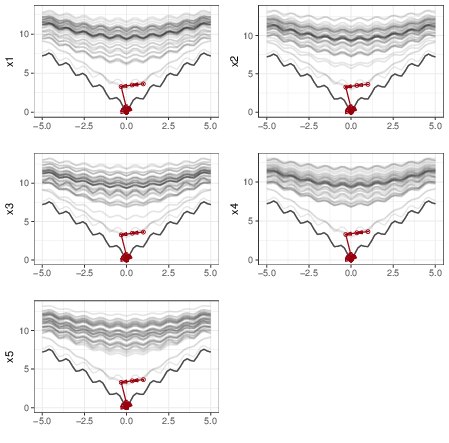
\includegraphics[width=\textwidth]{optim_trace_1_1.png}
    \subcaption{ 
      \label{fig:optim_1:sp}
    }
  \end{subfigure}
  \qquad\qquad
  \begin{subfigure}[b]{0.35\linewidth}
    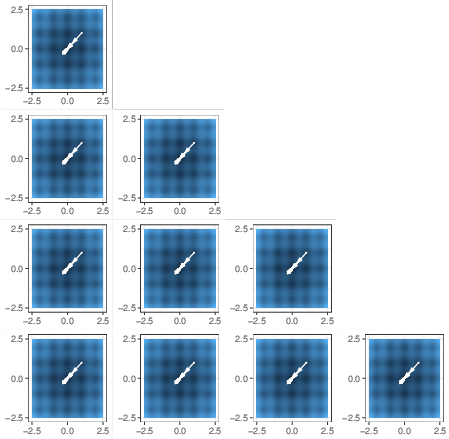
\includegraphics[width=\textwidth]{optim_trace_hs_1_1.png}
    %\resizebox{\textwidth}{!}{%
    %\begin{tabular}{rrrrr}
      %20.9885770  & -0.3256642 & -0.3257547 & -0.3258958 & -0.3252083 \\
      %-0.3256642  & 20.9908910 & -0.3254367 & -0.3255775 & -0.3248914 \\
      %-0.3257547  & -0.3254367 & 20.9902343 & -0.3256679 & -0.3249814 \\
      %-0.3258958  & -0.3255775 & -0.3256679 & 20.9892087 & -0.3251219 \\
      %-0.3252083 & -0.3248914 & -0.3249814 & -0.3251219 & 20.9941950
    %\end{tabular}
    %}
    \subcaption{
      \label{fig:optim_1:hs}
    }
  \end{subfigure}
  \\
  \begin{subfigure}[b]{0.35\linewidth}
    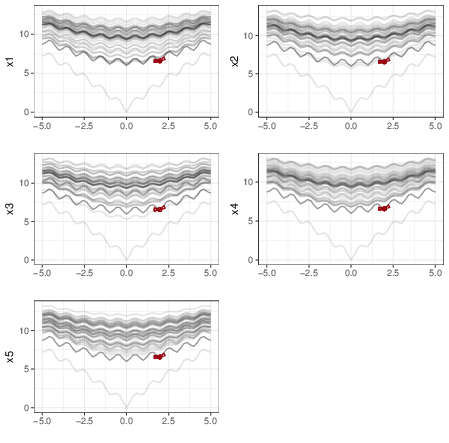
\includegraphics[width=\textwidth]{optim_trace_2_1.png}
    \subcaption{
      \label{fig:optim_2:sp}
    }
  \end{subfigure}
  \qquad\qquad
  \begin{subfigure}[b]{0.35\linewidth}
    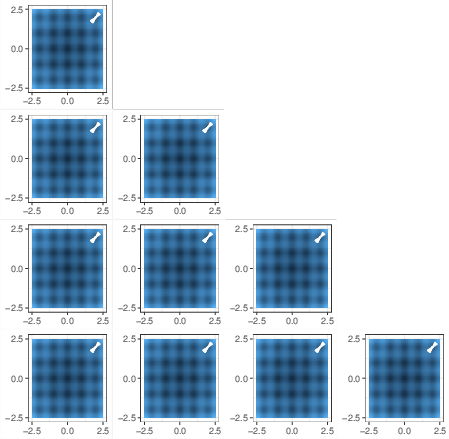
\includegraphics[width=\textwidth]{optim_trace_hs_2_1.png}
    %\resizebox{\textwidth}{!}{%
    %\begin{tabular}{rrrrr}
      %21.0042955 & -0.1840739 & -0.1843067 & -0.1846840 & -0.1845613 \\
      %-0.1840739 & 21.0067633 & -0.1839595 & -0.1843355 & -0.1842132 \\
      %-0.1843067 & -0.1839595 & 21.0051112 & -0.1845689 & -0.1844464 \\
      %-0.1846840 & -0.1843355 & -0.1845689 & 21.0024265 & -0.1848241 \\
      %-0.1845613 & -0.1842132 & -0.1844464 & -0.1848241 & 21.0033008
    %\end{tabular}
    %}
    \subcaption{
      \label{fig:optim_2:hs}
    }
  \end{subfigure}
  \caption{
    1D slice and HyperSlice views showing
    traces of an optimization algorithm searching for the global minimum
    of a 5D Ackley function.
    (\subref{fig:optim_1:sp}) and 
    (\subref{fig:optim_1:hs}) show the trace starting at the point
    $(1,1,1,1,1)$ while 
    (\subref{fig:optim_2:sp}) and 
    (\subref{fig:optim_2:hs}) 
    show the trace starting at the point $(2,2,2,2,2)$. 
  }
  \label{fig:optim_trace}
\end{figure}

The 1D slice view allows us to see the path that the algorithm took and the
general shape of the function simultaneously.  In addition, the 1D slice view
shows that the distribution of values around the global minimum is small. Most
of the slices are clustered around \(y=10\) with only one slice descending
close to \(y=0\). Since the sampling is uniform in the parameter space this
means that it is very difficult to select slices around the global minimum. In
fact, this is a known property of the Ackley function.  It is easy to see that
the optimization algorithm got stuck at a local minimum when started at
\(x=(2,2,2,2,2)\). However, with the HyperSlice view it is difficult to see the
difference in value and steepness of the function at \(x=(1,1,1,1,1)\) versus
\(x=(2,2,2,2,2)\).  Humans are not good at perceiving fine differences in
color~\cite{Munzner:2014}, but is required for this task. We learn a lot more
about the behavior of the optimization algorithm from the 1D slice views (see
\autoref{fig:optim_1:sp} and \autoref{fig:optim_2:sp}) than the HyperSlice
view. However, the HyperSlice view does clearly show that that optimization
algorithm is moving in multiple directions at once. This is not clear in the 1D
slice views.




\section{Discussion}

The above examples illustrated that the technique of 1D slices as presented are
quite flexible and useful for various low- and high-level tasks.  However, I do
not intend to claim that it is the only and best method for all problems out
there. Rather, I would like to argue that it is a valuable (and thus far
overlooked) technique in a toolbox of visual inspection methods for
multi-dimensional functions. I hope that this work inspires a discussion and
exploration of guidelines for tasks, proper visual encoding, and interaction
techniques for various application areas. Along these lines I would like to put
forth our current experience with various techniques.

\textbf{Topological techniques are helpful for a global overview}: Topological
techniques allow us to compare \emph{between} optima but are not as good at
evaluating the area \emph{around} an optimum since these areas are typically
abstracted away.  Topological spines attempts to compensate for this by showing
the area covered by a particular optimum as an area around the node. However,
many of the tasks like ``correlate'' and ``cluster'' are best served by viewing
the response manifold directly. In a larger system, the topological techniques
could be used effectively as a global overview of the function with a
HyperSlice or 1D slice showing local context. Selecting a point in the
topological view would change the focus point in the local view.

\textbf{HyperSlice is good when you need to show 2D interactions}: HyperSlice
is the only technique that can display more than one dimension of data
interaction.  So, if this is a requirement then HyperSlice is the best option.
However, one can use 1D slices to get a general overview of the dependence of
the function on each dimension. The dimensions that are not interesting
because, for example, the function is not sensitive to them could easily be
eliminated from further consideration. This would reduce the number of subplots
that we need to view in the HyperSlice plot.

\textbf{1D slices should be used for a ``first pass'' visualization}: 1D slices
addresses many of the tasks that a user wants to perform. The technique does a
very good job on a wide variety of tasks. 1D slices are easy to
implement, easy to understand, and the static view provides a lot of
information.


\section{Limitations and future work}
%\label{sec:limitations}

The 1D slice view consists of a projection of many lines.  the distribution of
slices are shown through direct projection. Techniques like contour
boxplots~\cite{Whitaker:2013} and curve boxplots~\cite{Mirzargar:2014} build a
distribution model of curves which could help to address the ``characterize
distribution'' task in \autoref{tbl:task_list}. However, neither of these or
any of the other time curve visualization techniques have been applied to
multi-dimensional functions. Evaluating these techniques for this purpose is an
exciting topic for future work.

When developing the 1D continuous slicing technique I only considered
multi-dimensional continuous scalar functions in terms of requirements, 
tasks, and comparisons. I do not consider multi-field 
(i.e.\ functions with multiple outputs) or complex-valued functions in the
analysis. There are multi-field topology techniques to address 
this~\cite{Duke:2012,Huettenberger:2014,Carr:2015} which I do not consider
but the technique and analysis would need to be extended to this domain.
This is left for future work.

The x-axis of each 1D slice is independent of the x-axes of the other 1D
slices. This allows each plot to scale individually if the range of inputs have
different values.  The x-axis and y-axis automatically change to incorporate
their respective minimum and maximum ranges. While the x-axis scales itself
independently, the y-axis is the same for each plot.  This is also the default
behavior in many of-the-shelf plotting packages. The plots will adjust
automatically to shifts.  For the x-axis we use axis-aligned projections.
Therefore, the views are sensitive to rotational transformations of the
function. 

Finally, the Sliceplorer technique is also based on sampling, just like the 
techniques used in the comparison.
As with any technique based on sampling one
must be careful to take an adequate number of samples in order to properly
capture all desired behavior.
%\ttwnote{add more about sampling limitations?}
If the function is not smooth we may see a slice that is an ``outlier,'' i.e.\
one slice is much higher or lower than all the others. In this case all other
slices will be compressed into either the top or bottom of the chart. This is
often a problem with many common visualization techniques like bar graphs or
scatterplots and can be addressed with log scaled axes, for example.



Understanding multi-dimensional spaces is difficult. Visualization can give
us context to help understand the geometry. With the direct visualization
of these multi-dimensional continuous datasets through slice views, we can
use a familiar concept to give context and meaning to a complex task.

Multi-dimensional continuous functions are commonly visualized with 2D slices
or topological views. With Sliceplorer, I explore 1D slices as an alternative
approach to show such functions. My goal with 1D slices is to combine the
benefits of topological views, that is, screen space efficiency, with those of
slices, that is a close resemblance of the underlying function.  I compare 1D
slices to 2D slices and topological views, first, by looking at their
performance with respect to common function analysis tasks. I also demonstrate
3 usage scenarios: the 2D sinc function, neural network regression, and
optimization traces. Based on this evaluation, I characterize the advantages
and drawbacks of each of these approaches, and show how interaction can be used
to overcome some of the shortcomings. 


I also presented Hypersliceplorer, an algorithm for generating 2D
slices of multi-dimensional shapes defined by a simplical mesh.  Often, slices
are generated by using a parametric form and then constraining parameters to
view the slice. In this case, I developed an algorithm to slice a simplical
mesh of any number of dimensions with a two-dimensional slice. In order to get
a global appreciation of the multi-dimensional object, I show multiple slices
by sampling a number of different slicing points and projecting the slices into
a single view per dimension pair. These slices are shown in an interactive
viewer which can switch between a global view (all slices) and a local view
(single slice). I show how this method can be used to study regular polytopes,
differences between spaces of polynomials, and multi-objective optimization
surfaces. 


Finally, I develop a method for predicting the rendering time to display
multi-dimensional data for the analysis of computer simulations using the
HyperSlice~\cite{Wijk:1993} method with Gaussian process model reconstruction.
My method relies on a theoretical understanding of how the data points are
drawn on slices and then fits the formula to a user's machine using practical
experiments.  I also describe the typical characteristics of data when
analyzing deterministic computer simulations as described by the statistics
community.  I then show the advantage of carefully considering how many data
points can be drawn in real time by proposing two approaches of how this
predictive formula can be used in a real-world system.


\subsection{Future}

My work has had a major focus on using direct visualization techniques to
understand multi-dimensional continuous spaces. My intention is that this work
can be expanded upon to herald in a new era of multi-dimensional data analysis.
In my opinion, the major innovations preventing this technique from being used
in a broader application are a library for slicing multi-dimensional spaces and
more user-focused projects.  Building on these two thrusts will move
multi-dimensional continuous data analysis to the mainstream.

One of the reasons for the lack of adoption for slice-based visualization of
multi-dimensional objects is the complete lack of software to generate even
static slice views. There are many libraries for popular data analysis
languages like Python, Javascript, and R. In order to make slice based views
more viable I plan to develop an interactive slice-based visualization software
based on the prototype tools I have already developed. This will lower the cost
of entry of slice-based views of multi-dimensional continuous datasets. The end
result is more users familiar with this visualization type.

In addition, more focused projects with end-users in the form of design
studies~\cite{Sedlmair:2012} will help to develop both the task taxonomy and
the visualization techniques. As part of the task abstraction, we can learn how
these users' tasks fit in with the task and data taxonomy proposed in this
thesis. Then we can refine and extend the task and data taxonomy. This taxonomy
will allow visualization researchers to identify gaps and develop tools to
address them, thus creating more effective visualizations of multi-dimensional
continuous data.


\subsection{Implications}

The main goal of my thesis was to explore what is possible with slice-based
visualizations of continuous multi-dimensional datasets. My hope is that this
work will serve as a basis for an increasing focus on direct visualization of
multi-dimensional objects. Often it seems that the default analysis technique
for more than three dimensions is to reduce
the dimensionality of the
data and then render the reduced data on screen. This suffers from issues of
distortion of distances and relative sizes. The analysis tasks for
multi-dimensional data are all developed around understanding the carefully
chosen dimensions. Hence, transforming these dimensions takes away a lot of
contextual knowledge about the simulation. 

I also hope to bring more attention to continuous multi-dimensional data analysis.
In the visualization community, most of the work on multi-dimensional and high-dimensional
data has focused on the discrete case. There are many task taxonomies, techniques,
and applications for discrete data. My hope with this thesis is that by developing
a task and data taxonomy as well as an in-depth study of direct visualization
techniques will bring similar attention to multi-dimensional continuous data
analysis. There are a number of under-explored application areas in this
field. I have identified some in my own work, but with further research in this
field will bring more knowledge and understanding about how we, as three-dimensional
beings can understand multi-dimensional continuous datasets.









\chapter{2D slices}
\label{chp:hypersliceplorer}

\begin{figure}
  \centering
  \begin{subfigure}[b]{0.45\linewidth}
    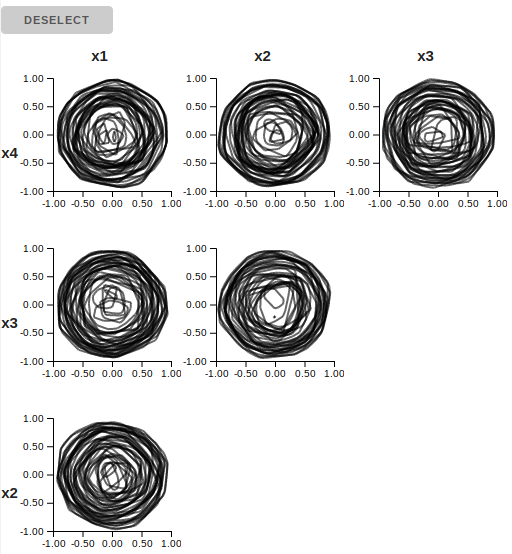
\includegraphics[width=\textwidth]{hsp_interface-global.png}
    \caption{Global view}
    \label{fig:interface:global} 
  \end{subfigure} 
  ~
  \begin{subfigure}[b]{0.45\linewidth}
    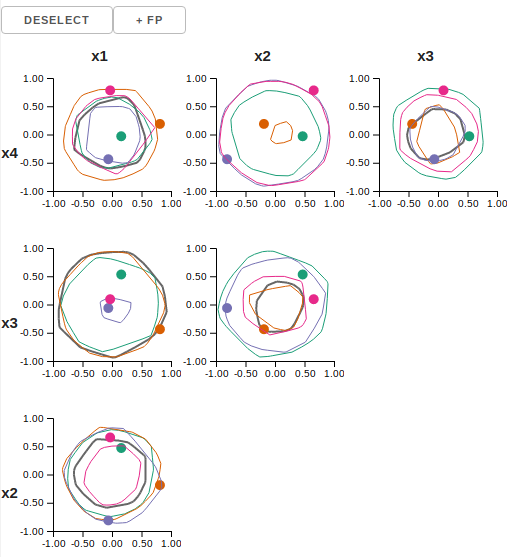
\includegraphics[width=\textwidth]{hsp_interface-local.png}
    \caption{Local view}
    \label{fig:interface:local} 
  \end{subfigure}
  \caption[The interface for browsing slices created by the Hypersliceplorer algorithm.]{%
    The interface for browsing slices created by the Hypersliceplorer algorithm.
    We show a plot for each pair of dimensions laid out in the same way as
    HyperSlice~\cite{Wijk:1993}.
    The interface has two modes: global and local view.
    The global view (\subref{fig:interface:global}) 
    shows the results of sampling over a number of focus points. The views
    are linked through highlighting a slice. The local view 
    (\subref{fig:interface:local}) shows a single selected slice and then
    the user can add additional slices by clicking the ``+ fp'' button.
  }
  \label{fig:interface}
\end{figure}

One-dimensional slices cannot do everything. When we are examining shapes then
we need to examine the relationship between dimensions. Thus, 2D slices are the
minimum number necessary to examine these relationships (see
\autoref{tbl:task_list}).  If we have a function describing the
multi-dimensional shape we are examining then we can generate two-dimensional
slices by constraining all but two of the parameters to a particular value and
then computing the two-dimensional outline directly. However, there are
domains, such as polytopes, where we have a simplical mesh of the continuous
object. In this case, we cannot use the dimension constraining method. In this
chapter, I develop an algorithm for generating two-dimensional slices of these
multi-dimensional simplical objects. 

%Thesis: Multi-dimensional spaces are better visualized through slice based views

We live in a three-dimensional world.  Ourselves and what we can interact with
are in three dimensions.  We learn about our world by studying the various
phenomena around us.  These phenomena are described as continuous processes.
In the beginning of our  education we study function plots in high school.
These give an intuitive view of one-dimensional phenomena.  By exploring the
relationship between an input factor
and output,
we can build an understanding on the relationship between the two.  We can also
compare one function plot to another. Visual inspection of these plots allows
us to see common patterns. We use our pattern recognition ability to quickly
categorize these different plots into different types of function behavior.
Function plots can also be used to describe two-dimensional phenomena. These
show the effect due to two input factors. In this case we can use the third
dimension or color encoding to show the function value.  From these plots we
can also make general statements about the ``shapes'' of the behavior like how
``peaky'' the function is or if it is monotonically increasing. These shapes
give us intuition into the underlying processes and help us learn about the
world~\cite{Palmer:1999}.

We also interact with many phenomena around us that are essentially
multi-dimensional in nature. For example, the weather in a certain location is
determined by the temperature, pressure, humidity, dew point, wind velocity,
and wind direction, among others. A change in any of the factors results in a
change in the weather. Each of these factors can be given a ``spatial
embedding.'' Then, they can be viewed as a dimension of some space.  By
``walking'' or navigating through this space we can observe the effect on the
weather due to changes in these parameters. 

Understanding multi-dimensional continuous spaces is difficult. As
three-dimensional beings we have real-world analogs for measurement, angle, and
position in three dimensions. We do not have these once we move beyond three
dimensions though. Nevertheless, visual analysis of these multi-dimensional
spaces has produced insights about the underlying
behavior~\cite{Sedlmair:2014,Gleicher:2016}. The issue is how to show more than
three dimensions on a two-dimensional screen. 

One strategy is to discretize the dataset through sampling and then use the
wealth of discrete visualization tools available. Much of the work on
multi-dimensional data analysis developed from analysis of 
tabular data. These datasets are often recorded from real-world
events such as census, species, or text data and contain many different aspects
about each entity. Thus, these datasets are inherently multi- or high-dimensional.
Each different aspect of the data items creates a dimension to be analyzed. 
In the case of these data the mental model is that of discrete objects
like humans, plants, or documents. Since the mental model is discrete in this
case it makes sense to use data processing and visualization tools designed for
discrete data.  However, our mental model for physical data is a continuous 
one. Therefore, the
discrete data paradigm breaks our mental model~\cite{Tory:2004a,Liu:2010a}. 
Breaking the mental model means that the visualization is not conveying the
complexities of the continuous phenomena.
Rather, we
should use visualization techniques purpose-built for continuous data.

While not as
extensively developed, there is previous work on visualizing multi-dimensional,
continuous data. These techniques can be broadly classified into projection,
topological, and slicing methods.  
Projection methods attempt to
distort the multi-dimensional object in order to view it on a two-dimensional
screen. With projection techniques we can preserve distance, direction, size,
or angles, but not all of 
these~\cite{Snyder:1987}. 
Depending on the
projection method, we may see radically different representations.  The issue
is that it is not clear from the resulting visualization what sort of
transformation was performed on the data.  Thus it can be difficult to
reconstruct the mental model of the multi-dimensional object.  One of the most
often seen multi-dimensional projection techniques is the Schlegel
diagram~\cite{Sommerville:1929} which picks a ``face'' of a polytope and projects the
remaining faces inside it. Thus, this technique only works for 4D polytopes.
Topological methods search the continuous dataset for values of interest, such
as critical points or contours.  Topological visualization techniques also
suffer from the issue of unclear transformation. It is difficult to relate the
resulting visualization back to features in the multi-dimensional object.

Slice-based views of multi-dimensional continuous spaces have not been explored
as extensively as other options.  This work began with the advent of
HyperSlice~\cite{Wijk:1993}.  HyperSlice extends the idea of slicing from
medical imaging to any number of dimensions.  HyperSlice provides the framework
for visualizing multi-dimensional continuous objects as a set of
two-dimensional slices.  There are $d \choose 2$ subpanels, one for each pair
of dimensions. Each panel shows a 2D slice of the object. The horizontal axis
shows one dimension and the vertical axis shows another dimension. Essentially,
each sub-plot of HyperSlice shows a 2D function plot. With 2D slices of solid
multi-dimensional objects color is often used to encode value. 

My work is inspired by the HyperSlice technique. Van Wijk and van Liere
introduced the idea of using slice-based views of multi-dimensional data.
However, they did not expand on what data types and tasks are involved in
multi-dimensional continuous data analysis.  I build on their work,
investigating the usefulness of slice-based views of continuous
multi-dimensional datasets. I also identified tasks involved in
multi-dimensional data analysis. The task analysis informed the development of
one- and two-dimensional slice-based views.

In this thesis I will explore
the possibilities of these slice-based views. Through a number of case
study examples, I will demonstrate the power of these views and ways to
address their shortcomings.

\subsection{Multi-dimensional spaces}
\label{sec:motivation:multi-d}

There are a number of domains where one can apply the analysis of continuous
multi-dimensional data.  As of yet, there has not been a comprehensive data and
task analysis for multi-dimensional continuous data analysis. For discrete
data, there are several task 
analyses~\cite{Shneiderman:1996,Brehmer:2013,Amar:2004}. 
However, they are
focused on identifying and selecting particular data items. Continuous datasets
consist of ranges of values as well as functions. Functions can be seen as a
mapping from ranges of numbers to other ranges. The analysis task here is to
study these ranges, their relationships to each other, and the mappings between
them. Tasks addressing these
have not yet been covered by visualization task analyses. Thus,
there is no comprehensive source for what analysis tasks one wants to perform
given a continuous multi-dimensional dataset.  Work in this area has
traditionally focused on developing a specific visualization for a specific
task. For example, topological spines extracts critical points from a scalar
field~\cite{Correa:2011}. One goal of this thesis is to develop this task
taxonomy for visualization of continuous multi-dimensional data.


These domains can be broadly classified into two types based on their analysis
tasks. One type, \emph{manifold} analysis, deals with understanding the
relationship between inputs and outputs. This is a functional relationship.
The user wants to inspect how changes in the inputs (independent variables)
affect the outputs (dependent variables). One can also perform \emph{shape}
analysis. Here, in terms of the analysis tasks, there is no identification of
independent and dependent variables. We look at each of these two in turn.

\subsection{Manifolds}
\label{sec:manifolds}

Studying the mapping between continuous ranges means studying functional
relationships and thus manifolds.  The critical issue is understanding the
relationship between independent and dependent variables.  Subtasks in manifold
analysis include examining critical points, assessing the sensitivity of
parameters, and understanding the shape of the manifold.  
One area where
understanding the manifold is important is analyzing optimization surfaces and
functions.  In this case, the identification of extrema is important for
understanding how many and the relative location of local optima. In addition,
we want to understand the degree to which these are extrema. These can result
in global optimization algorithms ``getting stuck'' in local optima rather than
continuing to search for the global optimum. Optimization algorithms need to be
carefully tuned to properly detect these features and ignore them where
necessary.

Simulations can be used to run experiments that are impractical or impossible
in the real world.  Simulation analysis is another area where the analysis
tasks, in the abstract, are examining functions. If we look back at the weather
simulation from before, the inputs to the function are things like the
temperature and pressure.  The output is, for example, the likelihood of rain
the next day. The function is the simulation itself. Computer simulations are
deterministic.  A deterministic simulation has a fixed mapping from each unique
input parameter configuration to an output value. This is the same as a
functional relationship. The sensitivity and extrema are also important to
simulation analysis.  Thus, these can all be analyzed with visualizations of a
manifold.

To date, manifold visualizations have concentrated on a particular analysis
task or a particular application domain. For example, visualizations of the
Morse-Smale complex~\cite{Gerber:2010} are focused on showing only critical
points of the manifold. As with any visualization designed for a specific task,
they must be used in combination with other views for visual analysis of
domain-specific data. Domain-specific visualizations often used linked views to
show different aspects of data to accomplish multiple tasks at once. However,
they are purpose built for a specific domain. While techniques may transfer
from one domain to another~\cite{Sedlmair:2012}, it is not always clear how.
My goal is to unify these methods to a certain extent.  As I will show in
\autoref{chp:sliceplorer}, slice-based views of manifolds can be used for a
wide variety of tasks in a wide number of domains.

\subsection{Shapes}
\label{sec:shapes}

One may also want to understand the relationship or correlation between
multiple continuous values. In the manifold analysis case we have the notion
of independent and dependent variables. This classification does not exist 
here.
In this case
we want to study the relationship of all variables. Careful study of the shape
of the dataset can give insight into the relationship between the various
ranges of dimensions of the object. For example, one may want to know if the
overall shape is a sphere, donut, or box. In addition one may be interested in
any kinks or cusps in the dataset. Changes in the gradient and curvature of
the shape are also of great interest. These indicate changes in correlation or
relation.

The analysis tasks of multi-dimensional shapes can be applied to a number of
different areas. The study of polytopes is one such area and perhaps the most
direct application of understanding multi-dimensional continuous shapes.
Polytopes are the multi-dimensional generalization of polyhedra and polygons.
The tasks are to understand the symmetries and patterns making up the
polytopes~\cite{Ziegler:2012}. Perhaps a less obvious connection is the
analysis of the tradeoff curves in multi-objective optimization. Since we are
performing optimization we are interested in the tradeoffs amongst all the
non-dominated points~\cite{Kung:1975}. This is also known as the Pareto
front. In this case, the user wants to understand what are the costs of
reducing one or more parameters in order to increase the value of others. Cusps
or large changes in curvature in these datasets are important since they show
critical changes in the rate of tradeoff.  With a proper view of a
multi-dimensional object we can also view differences between two objects
directly. 

These two different data types and sets of tasks require different visualization
considerations. Proper visualization for manifold analysis should focus on
the relationships between independent and dependent variables. Visualizations
of shapes do not have this mapping requirement and instead focus on the 
relationships between dimensions. With this categorization in mind, we can now
examine the available visualization techniques to examine these.


\subsection{Visualizing multi-dimensional continuous spaces}
\label{sec:multi-d-challenges}

Understanding multi-dimensional space is difficult. As humans, we simply do not
have the spatial analogs in more than three dimensions. A number of methods
have been developed to extract specific features from the multi-dimensional
object. For example, when studying polytopes, the number of faces and
symmetries is very important~\cite{Ziegler:2012}. However, these only produce
an answer without sufficient context. They do not necessarily give any
intuition as to how to transfer our three-dimensional knowledge to
multi-dimensional spaces.

Visualizations of multi-dimensional spaces on a 2D screen must contend with
some sort of reduction of the information. A proper visualization must select
visual encodings that highlight the information we want to see. Any sort of
data reduction requires trade-offs. The best visualization choices acknowledge
any deficiencies to a particular visual encoding. By acknowledging these
deficiencies, we can design tools to compensate for their shortcomings while
still maintaining their advantages. Therefore, it is worth first looking at the
possible mappings of data to visual elements. Then, I present commonly used
visual encodings of multi-dimensional continuous data using these mappings.

\subsection{Encoding multi-dimensional data}

Multi-dimensional continuous data consists of a set of continuous ranges, one
for each dimension. In the case of manifold analysis, each of these ranges can
be additionally classified as ``dependent'' or ``independent'' depending on
which side of the mapping they are on. Typical visualization practice is to
give each dimension a separate visual channel. There are a number of possible
visual channels that have been identified.  The ranking of effectiveness of
visual channels (shown in \autoref{tbl:visual_encodings}) was proposed by
Bertin~\cite{Bertin:1967} and confirmed through experiments by Cleveland and
McGill~\cite{Cleveland:1984}, Mackinlay~\cite{Mackinlay:1986}, and Heer and
Bostock~\cite{Heer:2010}.  Munzner~\cite{Munzner:2014} provides a summary of
the results. We are also limited in how many channels we can use
simultaneously. According to Ware~\cite{Ware:2004}, certain channels, such as
red and green are not visually separable. 

\begin{table}
  \caption{Rankings of visual encodings of quantitative data}
  \label{tbl:visual_encodings}
  \begin{adjustbox}{max width=\linewidth}
  \begin{tabular}{llll}
    Bertin~\cite{Bertin:1967} & Cleveland and McGill~\cite{Cleveland:1984} & Mackinlay~\cite{Mackinlay:1986} & Munzner~\cite{Munzner:2014} \\
    \hline \\
     Position & Position along a common scale & Position & Position on common scale \\
     Size & Position along identical, nonaligned scales & Length & Position on unaligned scale \\
     (Grey) Value & Length & Angle & Length (1D size) \\
     Texture & Direction & Slope & Tilt/angle \\
     Color & Angle & Area & Area (2D size) \\
     Orientation & Area & Volume & Depth (3D position) \\
     Shape & Volume & Density & Color luminance\\
     & Curvature & Color saturation & Color saturation \\
     & Densities & Color hue & Curvature \\
     & Shading & & Volume (3D size) \\
     & Color saturation &           & 
  \end{tabular}
  \end{adjustbox}
\end{table}

The difficulty of visualizing a continuous multi-dimensional space on a
two-dimensional screen brings a number of challenges. We treat each dimension
separately, thus, we need several different visual channels. However, there are
simply not enough visual channels available to draw a 15-dimensional object in
a single view. This is further complicated by the fact that separate visual
channels are not necessarily visually separable.  Furthermore, each dimension
of the multi-dimensional object under study is treated equally. For example, no
particular axis of a polytope is more important than any other.  We should
encode each dimension using equally weighted effectiveness channels.  With
fewer channels available than data dimensions we either need to reduce the data
or use multiple views to properly visualize the data.


\subsection{Methods}

The common taxonomy of how to view multi-dimensional data on screen is based on
discrete data analysis. There, there are two categories: dimension reduction or
projection. With continuous data, though there is a third possibility, that of
slicing. Therefore, I view the taxonomy of \emph{continuous} multi-dimensional
data analysis methods into two categories. Data-driven methods include both
projection and dimension reduction and reduce the dimensionality of the data
before visualization. View-based methods reduce the data during the
visualization. Slicing is a view-based method.

Purely data-driven methods are commonly known as feature selection or dimension
reduction. The goal is to find a subset of dimensions that are critical to
understanding the dataset. Topological techniques take this a step further.
They discard all spatial information about the dataset and only concentrate on
the difference in function value, as in the Morse-Smale
complex~\cite{Gyulassy:2012a}, or evolution of contours, as in the contour
tree~\cite{Carr:2003a}.  Projections also synthesize the dataset into new
dimensions to show using visual channels. Principal component
analysis~\cite{Holbrey:2006} is a popular choice in this area. This rotates the
space and thus produces new set of dimensions that are a linear combination of
the input dimensions. Even this relatively simple operation (a rotation) can be
difficult to understand. For example, iPCA~\cite{Jeong:2009a} was a tool to
help users understand the effects of the dimensional transformation.

View-based methods try and produce multiple linked views of a multi-dimensional
dataset from different angles. Each view shows a subset of the dimensions.
This way we can use a proper set of visual channels for each view.  We use
interaction to link these different views. These multiple, coordinated, linked
views have been one of the biggest success stories from the visualization
community~\cite{Rao:1994}. The traditional HyperSlice~\cite{Wijk:1993}
technique falls into this category. Each panel of the HyperSlice view shows two
of the input dimensions and the value is encoded with color.
The views are linked through the focus point selection. Changing the focus point
in one sub-plot updates the other sub-plots.

My work focuses on the exploration of the combination of data-driven and
view-based methods.  Data-driven methods reduce the data in a way that we can
get a global overview of the dataset. View-based methods are much more detailed
but can only produce a local view of the data. By combining these methods I can
achieve both a global overview as well as an on-demand local view of the
dataset in a single visualization. 


\subsection{Slices}
\label{sec:slicing-advantages}

Slicing offers a number of advantages over other multi-dimensional
visualization techniques. Slicing is a direct visualization of the
multi-dimensional object. In contrast to methods like projection or dimension
reduction, slicing does not distort the dimensions in order to display them on
a two-dimensional screen. Since there is no distortion, distances in the visual
representation are directly proportional to distances in the object. This is
one of the reasons that slicing is popular in the medical imaging community.
Sizes of organs or tumors can be measured visually on screen. Additionally,
relative sizes correspond to what a doctor would expect to see in the body.
Multi-dimensional data is abstract. It lacks the correspondence to real-world
objects that the medical community uses to understand their two- and
three-dimensional datasets. Nevertheless, it is still important in
multi-dimensional data analysis to properly estimate distances and relative
sizes. 

Another benefit of the direct visualization is that users do not require
extensive training to understand the visualization. The concept of slicing
through a three-dimensional object is a familiar one. Humans are used to this
even from slicing fruits and vegetables with a knife. This concept of slicing
can be extended from this well-known metaphor to cover multiple slices of
multi-dimensional objects.

Slice views use the horizontal and vertical axes for showing the effects due to
the input parameters. These axes are the most perceptually
uniform~\cite{Stevens:1957} and are considered the most effective
(\autoref{tbl:visual_encodings}). One- or two-dimensional
plots are replicated for each combination of dimensions in order to show more
than two dimensions at once. This promotes familiarity of the visualization.
Once the user has learned to read a single panel, they can apply this knowledge
to the remaining panels. This approach follows the principal of small
multiples~\cite{Archambault:2011}. 

In order to produce a slice plot one needs to first pick a particular
\emph{focus point} in the multi-dimensional space. This focus point determines
which slices are being viewed. Selecting a good focus point a-priori is
difficult. 
It either requires a great deal of luck or careful analysis of the
dataset. This is not always possible. Slice-based views require some sort of
interactive focus point selection. Interactively browsing through the slices
requires interaction controls to give the user control over the focus point.
Furthermore, we need some kind of navigation map to show which focus points the
user has selected so that they do not become lost. Neither of these navigation
aids are well developed at this point. This need for interaction is likely one
of the reasons that slice-based views have not developed as much as projection
or topological techniques. Static views are much easier to include in papers
and don't require explanation prior to use.

The other implementation issue of slice-based views is ensuring that the
visualization can remain interactive. In this case, interactive is defined as
the rate at which the user can maintain their
concentration~\cite{Shneiderman:1987}. This is often defined at 10 frames per
second. It can be difficult to compute a 2D slice of an arbitrary complex
multi-dimensional object. 


\subsection{Upcoming}
\label{sec:thesis_outline}

My goal is to highlight the advantages of slice-based methods for
multi-dimensional data analysis. At the same time I want to address the
limitations. The end goal is to bring slice-based views into the standard
toolbox of visualizations.

In \autoref{chp:sliceplorer}, I examine how to visualize manifolds using
slices. I present Sliceplorer which is a system to view one-dimensional slices
of multi-dimensional manifolds. I use projections of these one-dimensional
slices instead of showing one focus point at a time. I also go into detail
about the tasks one wants to perform with manifold analysis.

I extend the idea of projections of slices to the second dimension in
\autoref{chp:hypersliceplorer}.  I show how this can be used to effectively
visually analyze the shape of multi-dimensional data. In many cases, this data
is given as a simplical mesh. I introduce an algorithm to compute 2D slices of
this mesh.  Using this algorithm, I show how we can visually understand
datasets like Pareto fronts or polytopes.

Finally, in \autoref{chp:rendering}, I discuss how we can take advantage of the
multi-dimensional geometry and GPU architecture to allow interactive-speed
browsing of the focus points. In addition to this algorithm, I develop a method
that can predict the amount of time needed per element to draw one frame of the
visualization. I then show how this estimation formula can be calibrated to a
particular user's hardware.



\section{Related work}
\label{sec:related-work}

Multi-objective optimization and multi-dimensional objects are two areas
where it is important to study shapes in over three dimensions. We discuss 
these areas below. Topological techniques are based on viewing critical points
of manifolds~\cite{Correa:2011,Gerber:2010} or how contours merge and 
split~\cite{Carr:2003a}. We do not discuss them further. Manifold analysis
is very different than visualizing shapes. 

The need to understand multi-dimensional polytopes is apparent to 
geometers~\cite{Ziegler:2012}.
However, there are a number of cases in computational science where the
understanding of the size and the shape of a sub-section of the parameter space
is of importance~\cite{Bergner:2013,Sedlmair:2014}. One of these cases is
highlighted in \autoref{sec:bernstein}. Another use case is the study
of multi-dimensional Pareto fronts (\autoref{sec:pareto}).

\subsection{Multi-objective optimization}

In multi-objective optimization we have several scalar values that we wish to
optimize. The set of optimal points is known as the Pareto front.
If each objective measure is continuous then we have a continuous hull in one
orthant. We want to use this hull to analyze the trade-offs between objective
measures. Interactive decision maps~\cite{Lotov:2004} show a 3D Pareto front as
a series of 2D slices. Any objectives past three must be constrained to a value
however. Objective functions are difficult to sample since we often do
not have control over the sampling of the range of a function.  To
generate this hull one often samples the objective functions and then computes
the Pareto points using an algorithm such as NSGA-II~\cite{Deb:2002} or the
skyline algorithm~\cite{Borzsony:2001}. We can then generate the hull using
multi-dimensional marching cubes~\cite{Bhaniramka:2000}, the quickhull
algorithm~\cite{Barber:1996}, or alpha shapes~\cite{Edelsbrunner:1983}. These
can then be viewed in Hypersliceplorer as we do in \autoref{sec:pareto}.

An alternative is to treat the samples as a fixed set and then visualize the
relationship between possible combinations of objectives. Typically this is
done by examining the weight space through interaction. 
LineUp~\cite{Gratzl:2013} uses a ranked list approach and shows the user
how rankings will change as the user changes the relative weighting for each
objective. WeightLifter~\cite{Pajer:2016} extends this by also showing the
stability of rankings. The user can understand how much a particular objective
is affected by its weighting. This can help speed interactive exploration. 
Finally, the joint contour net~\cite{Carr:2014} can be used to compute how
often two objectives hold particular values simultaneously. 
In our case, the mental model is a continuous one. Thus it makes more sense
to show a continuous Pareto front.

\subsection{Multi-dimensional objects}

%TM: I wanted to add a sentence like this, but I dont think we need to after all: Since we are focusing on the visualization of continuous objects in multiple dimension, literature on projection based techniques is not relevant and will not be mentioned. 

%We review related work on the visualization of multi-dimensional continuous objects.

When speaking of 3D polytopes, their source is usually either from reconstruction of 3D point clouds 
(see Dey~\cite{Dey:2006})
or from iso-surfacing techniques (see Wenger~\cite{Wenger:2013}).
%However, we believe that the method of choice for visualization of 3D shapes are 3D renderings.
%Visualization of (continuous) objects in three (or fewer) dimensions is not that relevant for our discussion, since we believe that our method will not be of advantage here. Still, in the are of volume visualization there are quite a wealth of approaches for creating an iso-surface, which creates a 3D polytope. See also the excellent text books by Wenger or Day
%
%often falls under the name of
%volume visualization.  Three-dimensional volumes can be rendered using
%techniques isosurface techniques like marching cubes~\cite{Lorensen:1987a} or direct volume visualization. 
There are extensions to iso-surfacing techniques in multiple dimensions~\cite{Bhaniramka:2000}, 
%Marching cubes has been extended to arbitrary
%dimensions 
but in more than three dimensions we must distort the space somehow to visualize the object. 

For the visualization of 4D polytopes, there are a number of techniques for moving from four to three dimensions.  The
Schlegel diagram~\cite{Sommerville:1929} is one such method based on
projection. We pick a face of the figure, usually the largest, which is a
three-dimensional object. Then, all other faces are ``packed'' inside this face in
such a way that we can show the connections between faces. The Schlegel diagram
works well for regular polytopes where we have some previous intuition about
the faces. However, for an arbitrary simplical mesh, any face is a simplex
which we need to project into. All Schlegel diagrams of a simplical mesh look
like a simplex with a number of other simplices inside them. It can be
difficult to recover what the original object looks like because the
cross section is lost. An alternative approach is to treat the fourth dimension
as time and then produce an animation of the evolution of the shape in three
dimensions. In this case each frame of the animation is a 3D slice of the 
object. Rather than first projecting from 4D to 3D and then rendering the
projection, Hanson and Cross~\cite{Hanson:1993} propose a method to first
render the object in 4D and then view the three-dimensional projection. This
allows them to show unique lighting effects from the 4D surfaces.
%One can also use a stererographic projection. 
As with all projection methods, if the user is unaware of the details of the
method it can be difficult to build a mental model of the shape under study.

Hasse diagrams~\cite{Battista:1988} are based on showing the connectivity
between vertices of an object. These can be seen as network diagrams where the
vertices of the figure are the nodes in the graph and the edges of the graph
are the edges in the figure. These have a number of layout issues.  For visual
understanding, humans prefer a 2D planar graph~\cite{Kieffer:2016}. Good layouts
of the Hasse diagram must balance human aesthetic needs like few edge crossings
with the geometric interpretation. 
There are automatic layout
algorithms, such as the one by Battista et al.~\cite{Battista:1988}, but these
do not work in all cases.

For more than four dimensions, 
projection methods no longer work as well.  Techniques based on slicing the
space can be extended to any number of dimensions.  The techniques to perform
this so far, such as HyperSlice~\cite{Wijk:1993},
HyperMoVal~\cite{Piringer:2010}, and Sliceplorer~\cite{Torsney-Weir:2017a},
are designed to show slices of multi-dimensional manifolds.
They produce slices by
constraining all but two (for 2D slices) or one (for 1D slices) of the
dimensions to the focus point value and then producing a heatmap, contour plot,
or function plot. Sliceplorer addressed the focus point issue by sampling over
a number of focus points and projecting them down.  Exploded view
diagrams~\cite{Karpenko:2010} offer a hybrid method between a 3D volume
visualization and slicing.  However, they 
%also require a parametric description of the object under study and 
are limited to 3D objects. 
The global view of Hypersliceplorer is inspired by the idea of examining
cross sections. We also have a local
view which permits the user to look at a small number of self-selected slices.
We have developed a method to produce slices based on a simplical mesh which
is very useful given a discretized surface (see \autoref{fig:slicing}). 


\section{Algorithm}
\label{sec:algorithm}

\begin{figure*}[ht!]
  \centering
  \begin{subfigure}[b]{0.33\textwidth}
    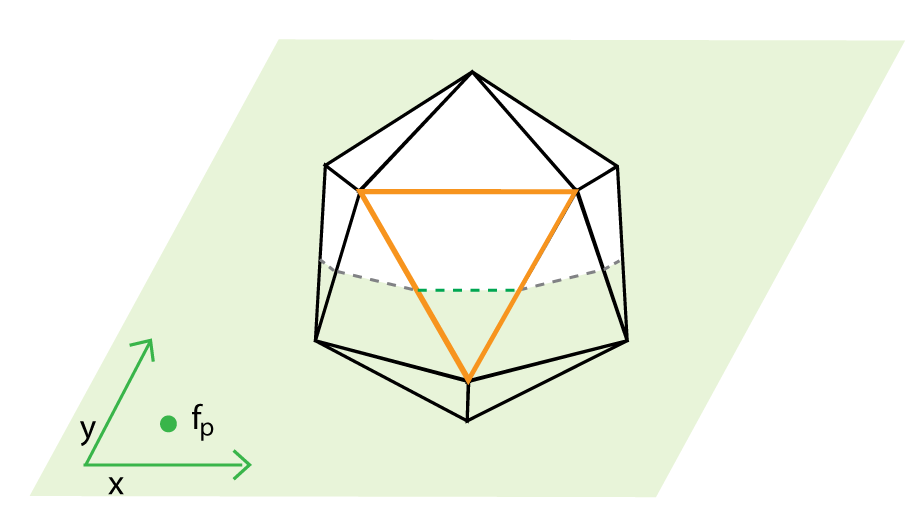
\includegraphics[width=\linewidth]{hsp_mesh-slicing.png}
    \caption{%
      Slicing a mesh
    }
    \label{fig:slicing:mesh}
  \end{subfigure}
  ~
  \begin{subfigure}[b]{0.33\textwidth}
    \centering
    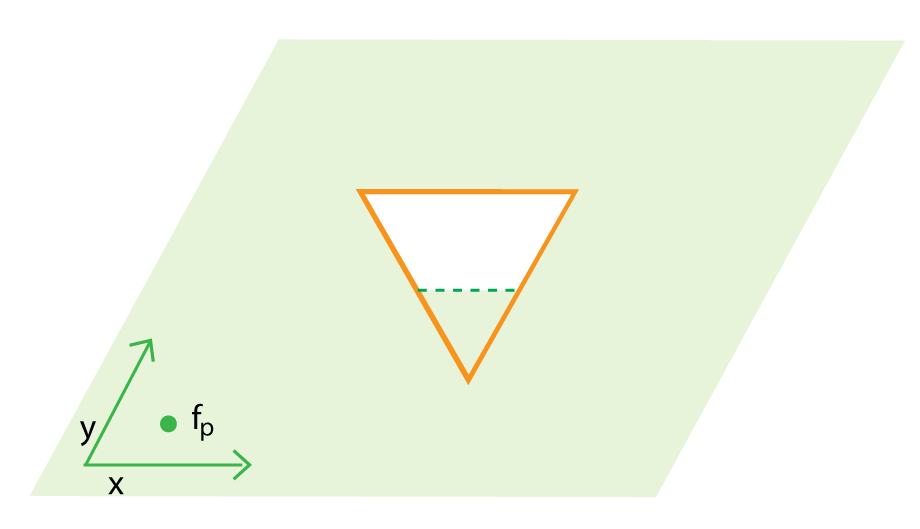
\includegraphics[width=\linewidth]{hsp_simplex-slicing.png}
    \caption{%
      Slicing a simplex
    }
    \label{fig:slicing:simplex}
  \end{subfigure}
  ~
  \begin{subfigure}[b]{0.24\textwidth}
    \centering
    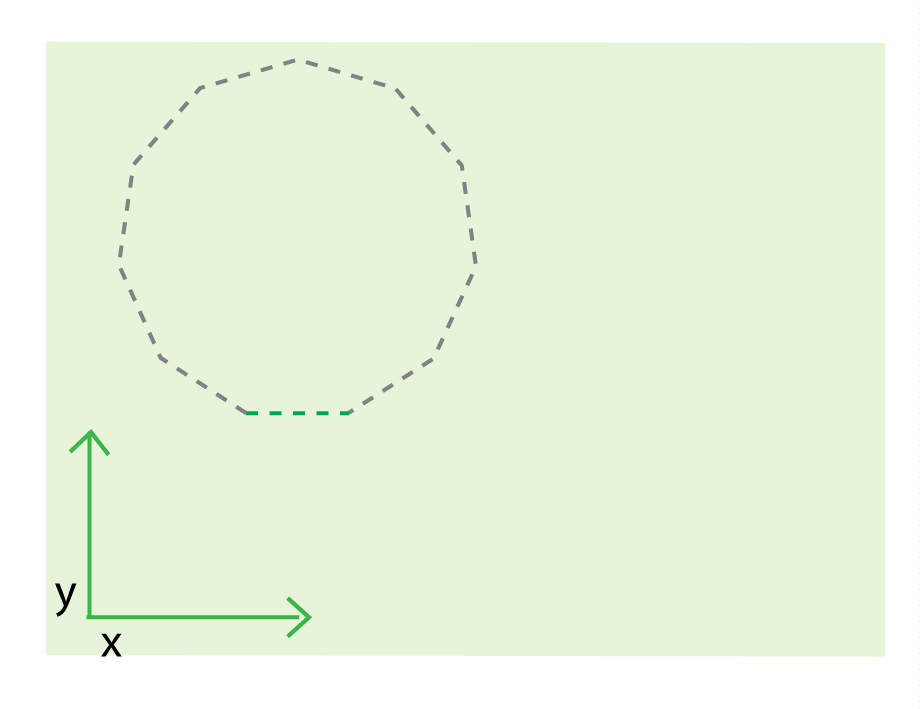
\includegraphics[width=\linewidth]{hsp_plane-slicing.png}
    \caption{%
      2D slice
    }
    \label{fig:slicing:plane}
  \end{subfigure}
  \caption{%
    An overview of how our algorithm functions. The goal is to compute the
    intersection of a slice with a polytope defined as a simplical mesh
    (\subref{fig:slicing:mesh}). The slice is defined by selecting a focus
    point and then extending it in two directions. We 
    (\subref{fig:slicing:simplex}) treat each simplex in the mesh 
    independently and compute the intersection of the simplex with the slice
    (see \autoref{alg:slicing:single}). The collection of all intersections
    for a particular plane is shown as a line plot 
    (\subref{fig:slicing:plane}). This process is repeated over a number of 
    randomly sampled focus points.
  }
  \label{fig:slicing}
\end{figure*}

%Now we turn to how we actually compute a two-dimensional slice of a
%multi-dimesnsional polytope.
There are a several ready-made solutions to creating a number of uniformly
distributed multi-dimensional samples (e.g.\ Sobol sequence~\cite{Sobol:1967}
or Latin hypercube~\cite{Mckay:1979}). These methods are based on ensuring that
the distance between sample points is as even as possible.  These will be our
focus points. Based on this, our main contribution is an algorithm
on how to slice a multi-dimensional polytope.  The algorithm will produce a
single two-dimensional axis-aligned slice for a single focus point. To produce
the full multi-dimensional view we repeat this algorithm for each focus point
and dimension pair.

\subsection{Conceptual overview}

Other slicing techniques, like Sliceplorer~\cite{Torsney-Weir:2017a} or
HyperSlice~\cite{Wijk:1993}, show slices of multi-dimensional manifolds.
In this case we can fix all but one or two of the
parameters, the parameters representing the slice, to a fixed value based on the
focus point. This gives us a two-dimensional function which we can draw as
a one- or two-dimensional function plot.

In our case, we have a simplical hull. This hull can be computed as a convex
hull of a point cloud using an algorithm such as quickhull~\cite{Barber:1996}
or they can be pre-defined.  In either case, a simplical hull is a set of
\(d-1\)-dimensional simplices for a \(d\)-dimensional space. 
A two-dimensional
slice is equivalent to a two-dimensional plane. So, in order to compute the
two-dimensional slice, we need to compute the intersection of a two-dimensional
plane with a set of \(d-1\)-dimensional simplices 
(see \autoref{fig:slicing:mesh}). 

The method often used in graphics for
computing a plane/simplex intersection is to represent the plane as a point and
normal vector. Then, we find the intersection by checking, for each pair of
points, if they are on opposite sides of the plane.
This works for 2D planes (slices) in 3D space
since the normal to the plane is unique. However, in more than three dimensions
we cannot use this method to compute the intersection of a 2D planar object.
This planar object does not have a well-defined concept of a ``side'' in a
multi-dimensional space. The analogy to this is a line in three-dimensions.

Our solution to this problem relies on two key observations. We can treat the
plane as a point with two free parameters and then see if
this point lies on the boundary of the simplex using barycentric coordinates.
A barycentric coordinate defines the location of a point on the face of a simplex.
%The plane must intersect the simplex
%at its boundaries. We express the position of a point within a simplex by using barycentric coordinates. 
For a single focus point, we choose a point somewhere in the domain. Then we
select two axis-aligned directions and create a plane by setting the values
of that point to free parameters, which we denote $x$ and $y$. These free parameters
create a 2D plane. We then want to see where this plane intersects the simplex
(\autoref{fig:slicing:simplex}). 
A point is located on the boundary of a simplex whenever at least one
barycentric coordinate is zero and the rest are between zero and one. 
If there is a solution then we will have a formula for the line segment
through the simplex (\autoref{alg:slicing:single}).
We compute these line segments for each plane/simplex intersection. The
collection of intersecting lines forms the image of the slice on the plane
(see \autoref{fig:slicing:plane}).

The simplical hull of a shape consists of $d−1$-dimensional simplices. However, in
order to convert to barycentric coordinates without using a pseudoinverse we
need a $d$-dimensional simplex where every point has a unique representation.
Therefore, we add the focus point as an extra vertex.  Now we have a
$d$-dimensional simplex. This will lead us to a square matrix, which is easy to
invert.  Any intersections with the extra point are removed at the end of the
algorithm.

\subsection{Algorithm details}

The algorithm requires that the shape we are slicing is specified as a set of
simplices. Each combination of simplex, pair of slicing dimensions, and focus
point is handled independently. These can be looped through, as in the
pseudocode (see \autoref{alg:slicing:all}), or in parallel, as in our actual
implementation.

To illustrate how our slicing algorithm works we first introduce some notation.  We begin with a $d$-dimensional focus point $f_p$ and a simplex $s$
consisting of $d+1$ $d$-dimensional points, $x_1, \ldots, x_{d+1}$. We denote
the slice as $f_p'$ in the formulas below. Without loss of generality, we will
assume the slicing dimensions to be $(d_1,d_2)=(1,2)$. Then, the two free
variables for the specification of the slice, $x$ and $y$, will replace the
first two components of the focus point (\autoref{eq:fp}). 
%\msnote{we might want to include 
%equations right at the spot. Imho this makes it easier to read. But maybe just a matter of style/taste ...}
We let $T$
be the matrix to convert a point from barycentric coordinates to Cartesian
coordinates (including a homogeneous component of 1). The columns of $T$ are the $d+1$ points defining the simplex. We append
a row of ones to ensure that the barycentric coordinates sum to one. The inverse
of $T$ will convert a point from Cartesian coordinates (including a homogeneous component of 1) back to barycentric coordinates.

\begin{align}
  f_p &= [p_1, p_2, \ldots, p_d,1] \\
  f'_p &= [x, y, p_3, \ldots, p_d, 1] \label{eq:fp} \\
  T &= 
    \begin{bmatrix}
      x_{1,1} & x_{2,1} & \cdots & x_{d+1,1} \\
      x_{1,2} & x_{2,2} & \cdots & x_{d+1,2} \\
      \vdots  & \vdots  & \ddots & \vdots    \\
      x_{1,d} & x_{2,d} & \cdots & x_{d+1,d} \\
      1       & 1       & \cdots & 1         
    \end{bmatrix} \\
\end{align}

The next step is to convert the slice, $f_p'$, to barycentric coordinates, 
$\lambda$.
\begin{align}
  T^{-1} &= 
    \begin{bmatrix}
      \alpha_{1,1} & \alpha_{2,1} & \cdots & \alpha_{d+1,1} \\
      \alpha_{1,2} & \alpha_{2,2} & \cdots & \alpha_{d+1,2} \\
      \vdots  & \vdots  & \ddots & \vdots    \\
      \alpha_{1,d+1} & \alpha_{2,d+1} & \cdots & \alpha_{d+1,d+1}
    \end{bmatrix} \\
  \lambda &= T^{-1} f'_p \\
          &= 
    \begin{bmatrix}
      \alpha_{1,1} x &+ \alpha_{2,1} y &+ \alpha_{3,1} p_3 &+ \cdots &+ \alpha_{d+1,1} \\
      \alpha_{1,2} x &+ \alpha_{2,2} y &+ \alpha_{3,2} p_3 &+ \cdots &+ \alpha_{d+1,2} \\
      \vdots \\
      \alpha_{1,d+1} x &+ \alpha_{2,d+1} y &+ \alpha_{3,d+1} p_3 &+ \cdots &+ \alpha_{d+1,d+1} \\
    \end{bmatrix}
    \label{eq:inverted}
\end{align}
This equation is essentially a linear equation in $x$ and $y$ and we denote its coefficients by $\lambda_x$, $\lambda_y$, and $\lambda_c$ respectively.
%If we look at $\lambda$, we will see that since there are two free parameters,
%each component of $\lambda$ will have a coefficient of $x$, coefficient of $y$,
%and a constant part. We let $\lambda_x$, $\lambda_y$, and $\lambda_c$ be each
%of these numbers respectively. 
Thus, each component is an equation of a line ($t$ is denoting the transpose).
\begin{align}
  \lambda_x &= \left[ \alpha_{1,1}, \alpha_{1,2}, \ldots, \alpha_{1,d+1} \right]^t \\
  \lambda_y &= \left[ \alpha_{2,1}, \alpha_{2,2}, \ldots, \alpha_{2,d+1} \right]^t \\
  \lambda_c &= \left[ \sum_{i=3}^{d+1} \alpha_{i,1} p'_i, \ldots, \sum_{i=3}^{d+1} \alpha_{i,d+1} p'_{d+1} \right]^t \\
  \lambda &= \lambda_x x + \lambda_y y + \lambda_c
\end{align}

Here, $x$ and $y$ correspond to the horizontal and vertical coordinates of the
intersection of the plane with the simplex. Each component of $\lambda$
reflects the influence of one of the ($d+1$) points of the simplex. If the
influence is zero (i.e. for the $i$-th point we have $\lambda_i=0$) then we are on
the boundary of the simplex.  An intersection of a plane with a
simplex must cross the boundaries
(\autoref{fig:slicing:simplex}) so it suffices to turn each
component of $\lambda$, $\lambda_i$, to zero in turn.  It is possible that the plane will
intersect multiple faces so we set each component of $\lambda$ to $0$ in turn
and then check what range of $x$ and $y$ in the remaining components are valid
barycentric coordinates (i.e.\ are between zero and one).  If this is the case,
then the plane intersects the simplex.  Otherwise, there is no intersection. In
other words, if we are trying to find the intersection for face $i$, we need to
solve $\lambda_i = 0$ such that $\forall j \ne i$, $0 \le \lambda_j \le 1$.
This can be solved either with a linear constraint solver or directly by
solving for $y$ setting $\lambda_i = 0$ and substituting it into each row $j$ of \autoref{eq:inverted}
%$\lambda_j$ 
and then finding an interval for $x$ and $y$ that allows each
$\lambda_j$ to be between $0$ and $1$.  We can do this by individually finding
the valid $x, y$ interval for each $j$ and then taking the intersection of all the
individual intervals. If the intersection is non-empty then this is the interval
of values for $x$ in the intersection. We can substitute this to find the
interval of values for $y$. We can then draw these intervals as line segments
on the screen (\autoref{fig:slicing:plane}). 

\begin{algorithm}
  \caption{Slicing a single simplex}
  \label{alg:slicing:single}
  \begin{algorithmic}
    \Function{slice}{$p$, $s$, $d_1$, $d_2$}
      \State $T\gets \left[ s\ 1 \right]^t$ \Comment{from barycentric to Cartesian coordinates}
      \State $r \gets p$
      \State $r[d_1,d_2] \gets [x,y]$
      %\State $r_c\gets p$ 
      %\State $r_c[d1,d2]\gets 0$
      %\State $r_x\gets \textbf{0}$
      %\State $r_y\gets \textbf{0}$
      %\State $r_x[d1]\gets 1$
      %\State $r_y[d2]\gets 1$
      %\State $\lambda_c \gets T^{-1} r_c$
      %\State $\lambda_x \gets T^{-1} r_x$
      %\State $\lambda_x \gets T^{-1} r_y$
      \State $\lambda_x x + \lambda_y y + \lambda_c \gets T^{-1} r$ \Comment{convert to barycentric coordinates}
      \State $\textrm{rng}_x \gets [-\infty,\infty]$
      \State $\textrm{rng}_y \gets [-\infty,\infty]$
      \For {$i\gets 1 \textrm{ to } d+1$} \Comment{each face of the simplex} 
        \State $(\textrm{rng}'_x,\textrm{rng}'_y) \gets$ \Call{solve}{$\lambda_{x,i} x + \lambda_{y,i} y + \lambda_{c,i} = 0, \textrm{s.t.} \forall j \ne i, 0 \le \lambda_{x,j} x + \lambda_{y,j} y + \lambda_{c,j} \le 1$}
        \State $\textrm{rng}_x \gets \textrm{rng}_x \cap \textrm{rng}'_x$
        \State $\textrm{rng}_y \gets \textrm{rng}_y \cap \textrm{rng}'_y$
      \EndFor
      \State \Return $\left( \textrm{rng}_x, \textrm{rng}_y \right)$
    \EndFunction
  \end{algorithmic}
\end{algorithm}

\begin{algorithm}
  \caption{Finding slices for all simplices}
  \label{alg:slicing:all}
  \begin{algorithmic}
    \For {$d_1=1 \textrm{ to } d-1$}
      \For {$d_2=d_1 \textrm{ to } d$} \Comment{all pairs of dimensions}
        \State $\textrm{slices} \gets [\varnothing,\varnothing,\varnothing,\varnothing]$ \Comment{4 column matrix for min/max $x$ and $y$}
        \For {$p \in FP$} \Comment{all focus points}
          \For {$s \in S$} \Comment{all simplices}
            \State $\textrm{ranges} \gets$ \Call{slice}{$p$, $s$, $d_1$, $d_2$}
            \If {$\textrm{ranges} \ne \emptyset$} \Comment{add new row if we found an intersection}
              \State $\textrm{slices} \gets \left[ \begin{matrix} \textrm{slices} \\ \textrm{ranges} \end{matrix} \right]$
            \EndIf
          \EndFor
        \EndFor
        \State \Call{plot}{$\textrm{slices}, d_1, d_2$} \Comment{plot slices to proper subplot}
      \EndFor
    \EndFor
  \end{algorithmic}
\end{algorithm}


\section{Interface}
\label{sec:interface}

I developed an interactive viewer to browse and select slices of interest in
order to build up an understanding of the object we are viewing. Slicing is an
inherently interactive operation. Depending on what focus point 
we will see different aspects of the data. In a multi-dimensional
space, it is easy to get lost navigating freely without guidance.
However, if we show all slices at once the user cannot closely examine one
particular aspect of the data.  Thus, the interactive interface, shown in
\autoref{fig:interface}, has two modes: a global view and a local view. The
global view is designed to give an overview of the general shape.  By selecting 
a slice and corresponding focus point of interest, the user can then
switch to the local view and gradually add additional slices at new focus
points.
%implementation?

\subsection{Global view}

The global view (\autoref{fig:interface:global}) gives an overview of the
possible cross sections of the object. By default we show slices for the first
50 focus points sampled using a Sobol sequence~\cite{Sobol:1967}. This has the
advantage of being both space-filling and easy to add additional sample points
if required. Since we are slicing hulls of simplicial meshes, each slice is a contiguous
line plot in the view. We use alpha blending in order to show the distribution
of hull shapes in each pair of dimensions. 
%We did this to show not only want to know which shapes are possible but also the frequency. 
From this the user can get insight into whether or not a shape has a regular 
structure.

With more than one slice one cannot easily tell how the slices correspond 
between panels in the layout. I address this by using linked highlighting
between the plots. If the user mouses over a slice in one plot the slices
corresponding to that focus point are highlighted in the other plots. In 
addition, the user can click on a particular slice of interest to focus in 
on that particular slice. This brings the user into the local view mode.

\subsection{Local view}

The local view mode of the interface allows the user to narrow in on a
particular focus point and then explore how other slices of the figure relate
to that one.  The focus point is represented as a dot projected on each sub
plot. 
%The user can drag this point to another focus point location which will then show the slice corresponding to that focus point.  
The user can change the focus point by dragging the
focus point dot to a new location. Thus, the user can change one or two focus
point values per dragging interaction.  The user can also add additional focus
points by clicking the ``+ fp'' button in the upper left of the interface. Each
focus point is automatically colored based on a discrete color map from
ColorBrewer~\cite{Harrower:2003}. The slices themselves and the focus points
are linked through a similar color.  For example, one mode of exploration this
view supports is examining the faces orthogonal to one of the slices.  The user
can return to the global view by clicking the ``deselect'' button on the top
left of the interface.



\section{Case studies}
\label{sec:case_studies}

Three areas where our method can be used is in the visual analysis of
multi-dimensional polytopes, differences between spaces, and multi-objective
optimization. We examine each of these in turn in the sections below.

\subsection{Polytopes}
\label{sec:polytopes}

%We can also use Hypersliceplorer to examine polytopes. 
Polytopes are the
generalization of polygons and polyhedra to any number of dimensions.
Naturally, in more than three dimensions we have no way of viewing these
objects directly. Common ways to view them is either through
projections, such as the Schlegel diagram~\cite{Sommerville:1929}, or as a
graph representation, like the Hasse diagram~\cite{Battista:1988}. Projection
methods do not accurately show distances or angles. These must be distorted to
show a multi-dimensional object in two or three dimensions. Network diagrams do
not necessarily show symmetries or structure unless care is taken during
layout.

\begin{figure} 
  \centering
  \begin{subfigure}[b]{0.45\linewidth}
    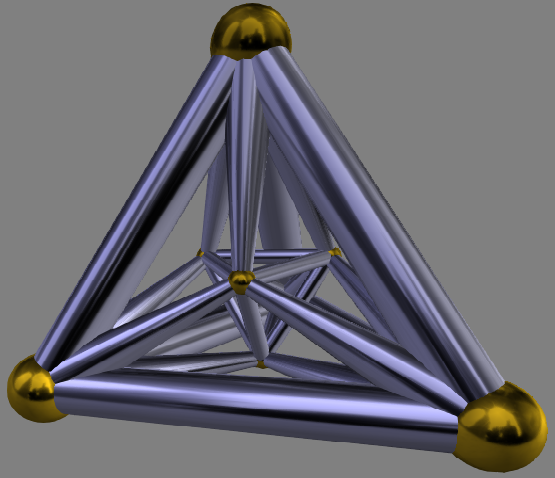
\includegraphics[width=\textwidth]{hsp_16cell-schlegel.png}
    \caption{Schlegel diagram: 16-cell (4D) generated using Stella4D~\cite{Stella4D}}
    \label{fig:ortho:schlegel} 
  \end{subfigure} 
  ~
  \begin{subfigure}[b]{0.45\linewidth}
    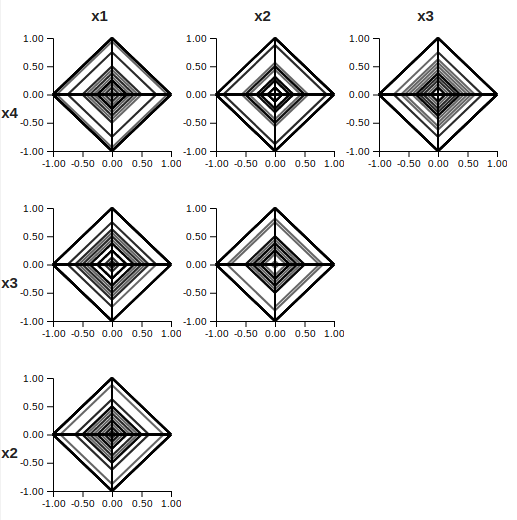
\includegraphics[width=\textwidth]{hsp_16cell-global.png}
    \caption{Hypersliceplorer: 16-cell (4D)}
    \label{fig:ortho:4} 
  \end{subfigure}
  \\
  \begin{subfigure}[b]{0.45\linewidth}
    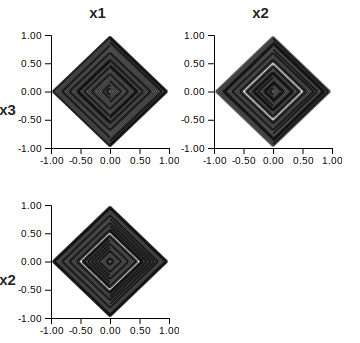
\includegraphics[width=\textwidth]{hsp_octo-global.png}
    \caption{Hypersliceplorer: Octahedron (3D)}
    \label{fig:ortho:3} 
  \end{subfigure}
  ~
  \begin{subfigure}[b]{0.45\linewidth}
    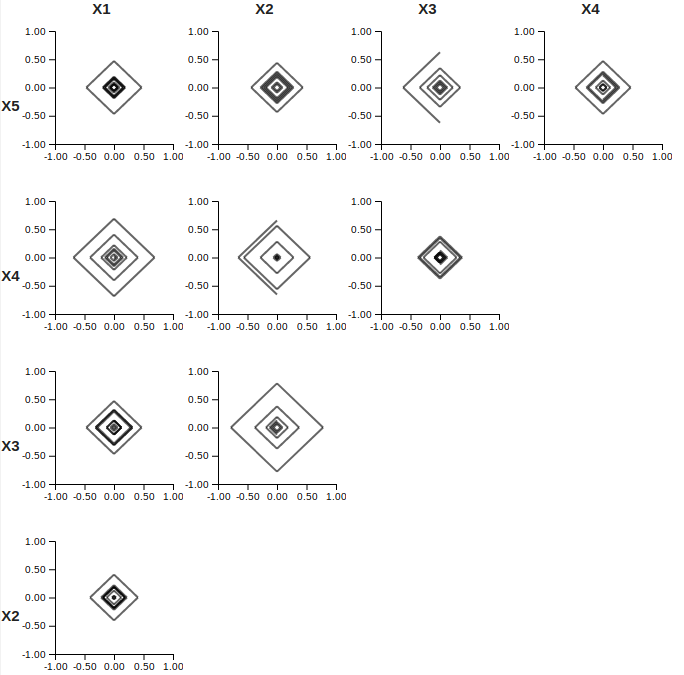
\includegraphics[width=\textwidth]{hsp_5ortho-global.png}
    \caption{Hypersliceplorer: 5-orthoplex (5D)}
    \label{fig:ortho:5} 
  \end{subfigure} 
  \caption{%
    This figure shows the 16-cell, the 4-dimensional regular orthoplex (4D 
    version of
    an octahedron) as (\subref{fig:ortho:schlegel}) a Schlegel diagram and
    (\subref{fig:ortho:4}) the Hypersliceplorer view. The Hypersliceplorer
    view shows the outside shape of the figure and the repeating structure.
    We can also see the repeating structure in the 3D (\subref{fig:ortho:3})
    and 5D (\subref{fig:ortho:5}) views.
  } 
  \label{fig:orthos} 
\end{figure}

As an alternative, we can slice these polytopes and examine the slices.
Regular polytopes have well-studied structure and symmetries so I use these as
verification examples. I examine these with Hypersliceplorer and see if the
structure matches reality.  For example, in \autoref{fig:orthos} I show a
16-cell which is the four-dimensional version of an octahedron in both
Hypersliceplorer (\autoref{fig:ortho:4}) and as a Schlegel diagram (\autoref{fig:ortho:schlegel})
using the Stella4D software~\cite{Stella4D}. The
Schlegel diagram picks a face of the 16-cell and projects the remaining
structure inside it. In this case, each face of the 16-cell is a simplex. From
the Schlegel diagram it is difficult to see that the dual of the 16-cell is the
hypercube (i.e.\ each vertex of the hypercube corresponds to a face of the 16-cell and vice
versa). However, in Hypersliceplorer this property is clear from looking at the
cross sections. We can see that each cross section looks like a rotated cube
which comes from the dual property. In addition, we can see the simplical faces
from the horizontal and vertical lines in the view. These result from intersections of the
2D slice with a face of the 16-cell directly.

Further, Hypersliceplorer allows us the visualization 3D or 5D analogs of the 16-cell (the octahedron in 3D, \autoref{fig:ortho:3}, as well as the 5-orthoplex in 5D, \autoref{fig:ortho:5}). The Schlegel diagrams cannot be scaled to higher dimensions.

We can also look at other regular polytopes in the same fashion. 
\autoref{fig:cubes} shows a hypercube in 3-, 4-, and 5-dimensions. From these
plots we can clearly see the generalization of the square, to the cube, to
higher dimensions. One of the advantages of my method is that I do not need
to choose a face to project into. For example, with a discretized hypersphere,
there are many faces. We can see in \autoref{fig:spheres} the regular cross
section of a sphere as well. 

\begin{figure} 
  \centering
  \begin{subfigure}[b]{0.3\linewidth}
    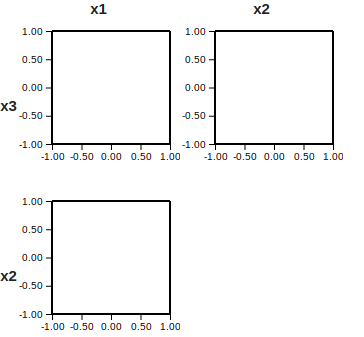
\includegraphics[width=\textwidth]{hsp_3cube.png}
    \caption{3D}
    \label{fig:cubes:3d} 
  \end{subfigure} 
  ~
  \begin{subfigure}[b]{0.3\linewidth}
    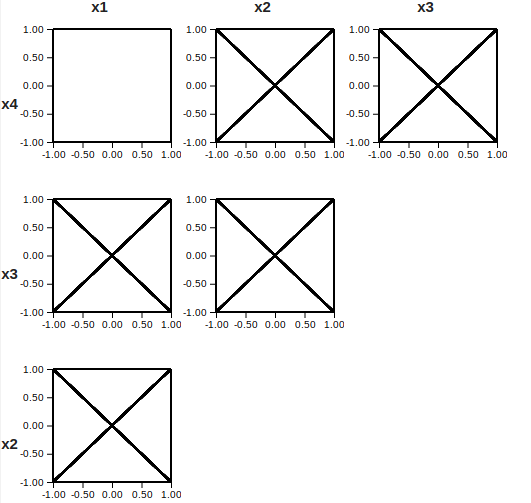
\includegraphics[width=\textwidth]{hsp_4cube.png}
    \caption{4D}
    \label{fig:cubes:4d} 
  \end{subfigure}
  ~
  \begin{subfigure}[b]{0.3\linewidth}
    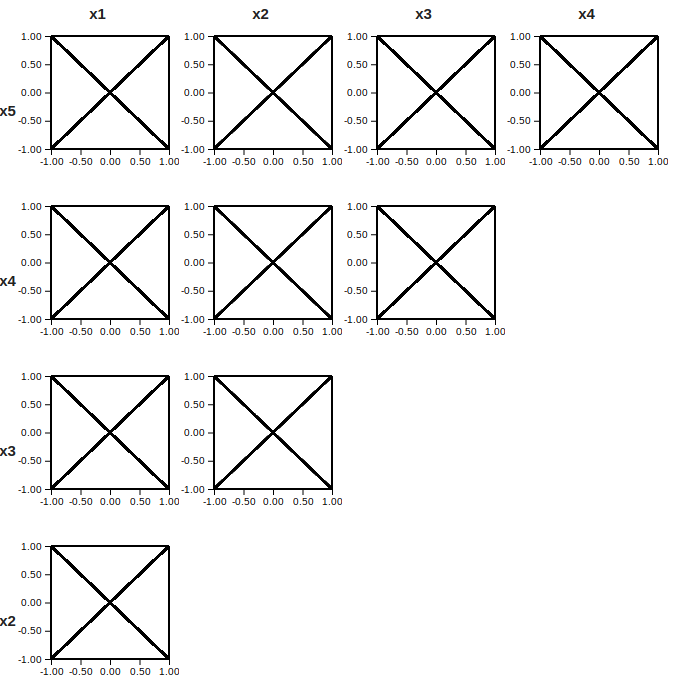
\includegraphics[width=\textwidth]{hsp_5cube.png}
    \caption{5D}
    \label{fig:cubes:5d} 
  \end{subfigure}
  \caption{%
    3-, 4-, and 5-dimensional hypercubes. We can see the regular structure
    in the cubes. The cross sections are all the same size since the cube
    is oriented to the axes. The cross lines in the plots are due to the 
    simplical mesh.
  } 
  \label{fig:cubes} 
\end{figure}

\begin{figure} 
  \centering
  \begin{subfigure}[b]{0.3\linewidth}
    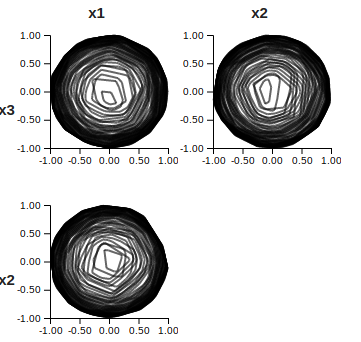
\includegraphics[width=\textwidth]{hsp_sphere_3d.png}
    \caption{3D}
    \label{fig:spheres:3d} 
  \end{subfigure} 
  ~
  \begin{subfigure}[b]{0.3\linewidth}
    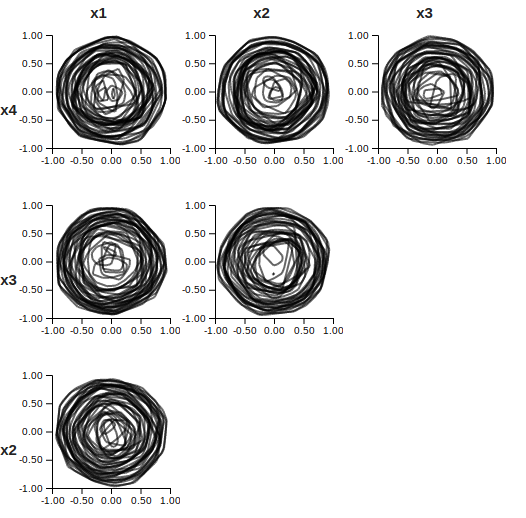
\includegraphics[width=\textwidth]{hsp_sphere_4d.png}
    \caption{4D}
    \label{fig:spheres:4d} 
  \end{subfigure}
  ~
  \begin{subfigure}[b]{0.3\linewidth}
    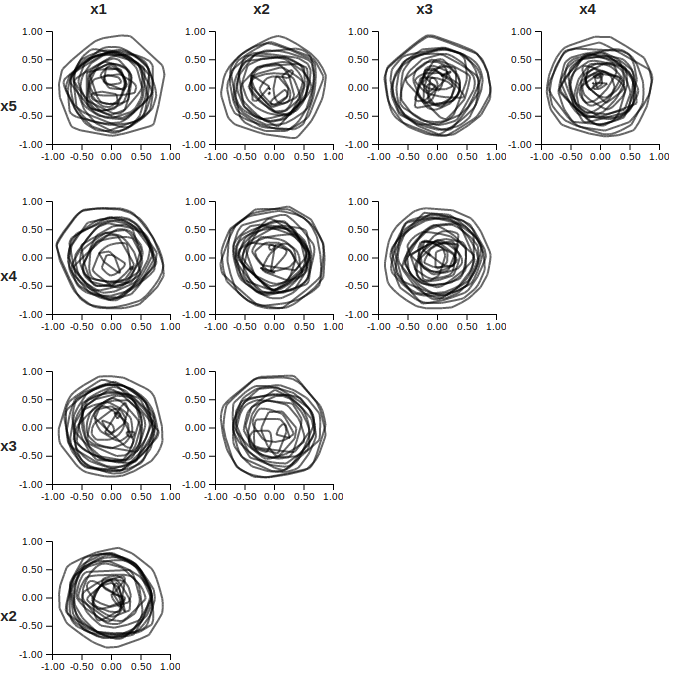
\includegraphics[width=\textwidth]{hsp_sphere_5d.png}
    \caption{5D}
    \label{fig:spheres:5d} 
  \end{subfigure}
  \caption{%
    3-, 4-, and 5-dimensional hyperspheres. We can see the concentric rings
    from slicing the sphere at different points. The irregularity of the
    slices is due to sampling.
  } 
  \label{fig:spheres} 
\end{figure}



\subsection{Positive and Bernstein polynomials}
\label{sec:bernstein}

In physics, it is sometimes necessary to fit data with a function that is
positive everywhere on its domain.  An example of such data is density; it
is a positive quantity and any regression on it should be positive.  In
numerical methods, we often use polynomials as a means of representation, and
hence we want to find polynomials that are positive on some compact domain,
without loss of generality say, $[0,1]$.
It is very difficult to control a polynomial
such that it is positive during the fitting process using a linear constraint
solver. One method used by physicists is to restrict the
fitting process to Bernstein polynomials~\cite{Phillips:2003}. By only using 
positive Bernstein coefficients, Bernstein
polynomials are restricted to be strictly positive.  However,
%based on our interviews with experts,
physicists do not know how ``representative'' are the positive Bernstein
expansions of the space of positive polynomials. In other words, can every
positive polynomial be represented by a corresponding Bernstein polynomial? 
To show these differences, I
select a large number of polynomials and visually compare the spaces in
order to understand the differences.

A Bernstein polynomial of degree \(n\) is a linear combination of
\(n+1\) basis polynomials. 
\[
B_n(x) = \sum_{i=0}^n \beta_i b_{i,n}(x) 
\]
where \(\beta_i\) is a scalar factor and
\(b_{i,n}\) is a Bernstein basis polynomial. These are defined as, 
\[
b_{i,n}(x) = {n \choose i} x^i (1-x)^{n-i}.
\] Each of the
Bernstein basis polynomials is positive in the range \([0,1]\), therefore
if we constrain all \(\beta_i \ge 0\) then the resulting polynomial will
also be positive.

\subsubsection{Sampling method}

The space of a polynomial of degree \(n\) is the range of each of its
coefficients. For example, a 2\textsuperscript{nd} degree polynomial, \(a_0 +
a_1 x + a_2 x^2\), has three coefficients: \(a_0\), \(a_1\), and \(a_2\).
Since we are only concerned with positivity, any polynomials that differ from
each other by a positive factor are equivalent. Thus, the polynomials $0.2x^2 +
0.1x + 2$ and $0.1x^2 + 0.05x + 1$ will be positive in the same range.
Therefore, I constrain the sampling by setting one of the coefficients to $1$
or $-1$ and then sampling the rest between $-1$ and $1$.  I used $10,000$
sample points to get a representative sample.  Since one coefficient is
constrained in turn to either \(-1\) and \(1\) there are \(2n\) possible
polynomials where the remaining \(n\) coefficients range between \([-1,1]\). I
then test to see if each polynomial is positive in the domain \([0,1]\). I also
determine if the equivalent Bernstein polynomial has all \(\beta_i \ge 0\). We
can compute the \(\beta_i\) factors because each coefficient \(a_j\) is a
linear combination of Bernstein coefficients. For our two-dimensional example:
\(a_0 = \beta_0\), \(a_1 = 2(\beta_0-\beta_1)\), and \(a_2=\beta_0 - 2\beta_1 +
\beta_2\). Then, for each polynomial, it is either non-positive, positive
without positive Bernstein coefficients, or positive with positive Bernstein
coefficients. I perform this process to examine polynomials of degree 3, 4, and
5. Constraining a coefficient to $\pm 1$ produces a face of the space of
polynomials. These faces are convex so I can generate a convex hull of these
points and examine them using Hypersliceplorer. Since we are only interested in
how these spaces differ, we examine the difference views.

\begin{figure}
  \centering
  \begin{subfigure}[b]{0.45\linewidth}
    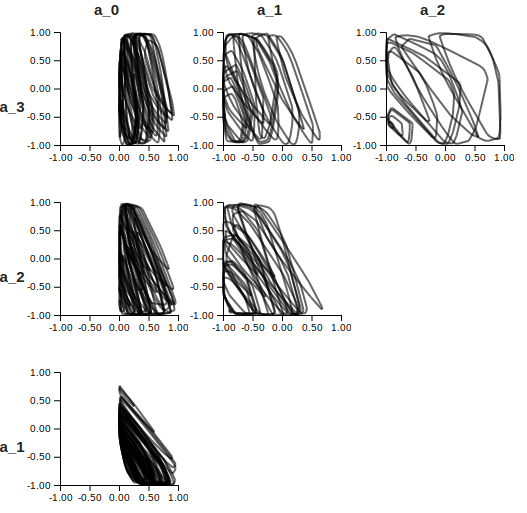
\includegraphics[width=\textwidth]{hsp_d5f1_4-global.png}
    \caption{global view}
    \label{fig:spacediff:global}
  \end{subfigure}
  ~
  \begin{subfigure}[b]{0.45\linewidth}
    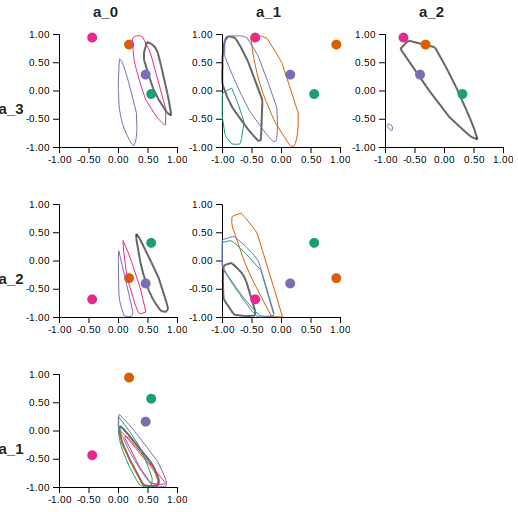
\includegraphics[width=\textwidth]{hsp_d5f1_4-local.png}
    \caption{local view}
    \label{fig:spacediff:local}
  \end{subfigure}
  \caption[Using Hypersliceplorer to examine differences in spaces]{%
    The difference between possible coefficient values for general positive 
    polynomials, $a_0 + a_1 x + a_2 x^2 + a_3 x^3 + x^4$, and polynomials
    that can be represented with positive Bernstein coefficients. From the 
    global view (\subref{fig:spacediff:global}) we can see that the 
    area of the slices is quite large. This means that the 
    difference between spaces is quite large, especially with respect to the
    higher-order coefficients. We can narrow into a particular slice in
    the local view (\subref{fig:spacediff:local}) we can see 
    the orthogonal faces to the slice in the $a_2 \times a_3$ plot.
  }
  \label{fig:spacediff}
\end{figure}

The current assumptions is that, while there is a difference between the set of all positive polynomials and the set of all Bernstein polynomials with positive coefficients,
that difference is small. However, the Hypersliceplorer visualization shows
that this is not the case. \autoref{fig:spacediff:global} 
shows all 4\textsuperscript{th} degree polynomial with the $x^4$ term fixed to
$1$. We can see that for almost an entire range of the $x^2$ and $x^3$
coefficients $a_1, a_2$ there are positive polynomials for which one cannot find a
Bernstein polynomial with positive Bernstein coefficients. Using the local view
(\autoref{fig:spacediff:local}), we can see that this difference is also
large in the other dimensions. Other patterns become apparent, such that $a_0>0$ which could lead to novel hypothesis that can be tested.

\begin{figure*}
  \centering
  \begin{subfigure}[b]{0.3\textwidth}
    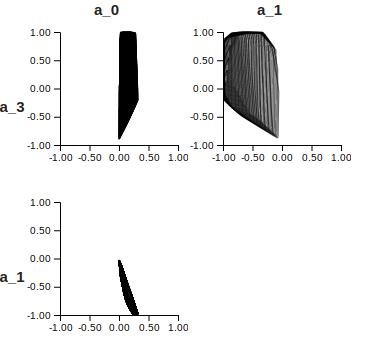
\includegraphics[width=\textwidth]{hsp_d3f1_3.png}
    \caption{degree 3 polynomials}
    \label{fig:dimcmp:3}
  \end{subfigure}
  ~
  \begin{subfigure}[b]{0.3\textwidth}
    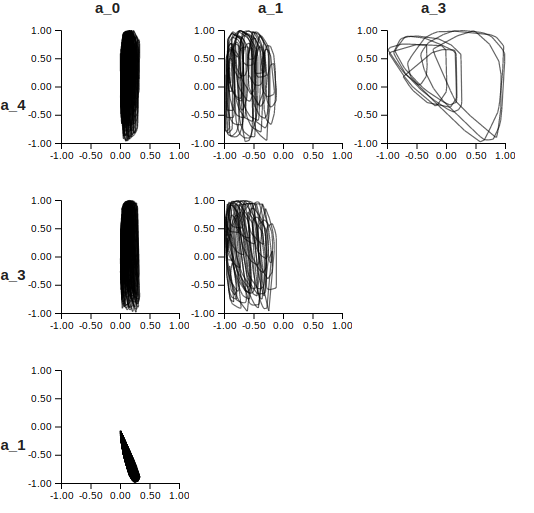
\includegraphics[width=\textwidth]{hsp_d3f1_4.png}
    \caption{degree 4 polynomials}
    \label{fig:dimcmp:4}
  \end{subfigure}
  ~
  \begin{subfigure}[b]{0.3\textwidth}
    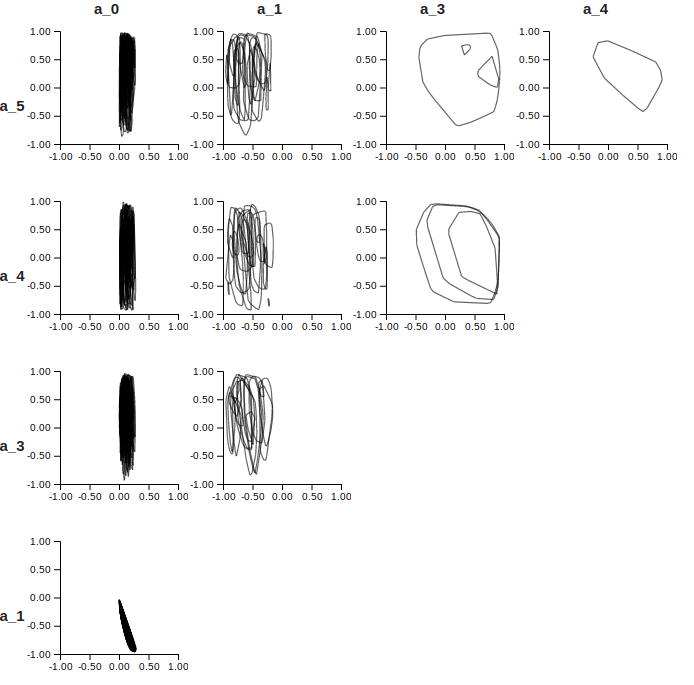
\includegraphics[width=\textwidth]{hsp_d3f1_5.png}
    \caption{degree 5 polynomials}
    \label{fig:dimcmp:5}
  \end{subfigure}
  \caption[Differences in the space of general positive polynomials and Bernstein polynomials with positive Bernstein coefficients.]{%
    Examining differences in the space of general positive polynomials and Bernstein 
    polynomials with positive Bernstein coefficients. In this example the 
    $x^2$ term is set to $1$. We can see that across degrees of polynomials,
    the space differences in the $a_0$ and $a_1$ coefficients is relatively
    consistent. The empty plot in \subref{fig:dimcmp:5} for the $a_3$, $a_4$
    plot is because the focus point sampling did not hit a particular slice.
    The solution is to add additional focus point samples. 
  }
  \label{fig:dimcmp}
\end{figure*}

The global overview also lets us compare across degrees of polynomials.
In \autoref{fig:dimcmp} I show a 3\textsuperscript{rd}, 4\textsuperscript{th},
and 5\textsuperscript{th} degree polynomial with the coefficient of the $x^2$
term set to $1$. Here we can see that the $a_0 \times a_1$ plots all look the same.
In fact, the width across all the panels including $a_0$ are the same. In this
case this means that for these ranges of $a_0$ (the constant term) we will not
be able to find a Bernstein polynomial with positive Bernstein coefficients
no matter the degree of polynomial. 
%\ttwnote{This is because the polynomial coefficients aren't made by that many 
%Bernstein coefficients. Work out the details.}
%\ttwnote{mk: you should be able to use a uniqueness argument.  If you have N+1 points, there is only one polynomial that interpolates it -- a polynomial of degree <= N.  The representation can be monomials, Bernstein, etc.  So, once you "pin" a polynomial (expressed in a monomial expansion), there is but one Bernstein expansion that exists for it; it either has all positive coefficients or not.}



\subsection{Pareto fronts}
\label{sec:pareto}

\begin{figure} 
  \centering
  \begin{subfigure}[b]{0.45\linewidth}
    \includegraphics[width=\textwidth]{hsp_3d_pareto.png}
    \caption{3D}
    \label{fig:pareto:3d} 
  \end{subfigure} 
  ~
  \begin{subfigure}[b]{0.45\linewidth}
    \includegraphics[width=\textwidth]{hsp_5d_pareto.png}
    \caption{5D}
    \label{fig:pareto:5d} 
  \end{subfigure}
  \caption{%
    Hypersliceplorer views of spherical Pareto fronts in 3D 
    (\subref{fig:pareto:3d}) and 5D (\subref{fig:pareto:5d}). 
    The smoothest possible Pareto front is the positive orthant of a 
    hypersphere.  From
    the Hypersliceplorer view we can clearly see the concentric arcs. Each
    arc allows the user to compare the trade-offs between two objectives 
    given that all other objectives are fixed. Changing from one arc to 
    another means changing other objective settings.
  }
  \label{fig:paretoex}
\end{figure}

%We can also use Hypersliceplorer to visualize the Pareto front used to
%understand trade-offs in multi-objective optimization. 
A Pareto front (also
known as the efficient frontier) is the set of all points that are optimal with
respect to some trade-off between objectives. Algorithms such as the skyline
algorithm~\cite{Borzsony:2001} or NSGA-II~\cite{Deb:2002} can extract these
points automatically. The issue with multi-objective optimization is this
trade-off is not always known. Thus visual analysis of the trade-offs is
necessary. With two objectives, this can be visualized using a scatterplot or
line plot of the two objectives against each other. 

In more than two dimensions this is no longer a curve, it is a hull. The common
technique is to use a scatterplot matrix with discretely sampled points. This, however, hides the trade-offs between
points in the other dimensions. Instead, we can examine the hull of the 
Pareto front by slicing using Hypersliceplorer.

The smoothest possible Pareto front is a sphere in the positive orthant of the objective
space. In order to illustrate our technique we show a 3D and 5D
positive orthant section of a sphere in \autoref{fig:paretoex}.  Each arc is
the trade-off holding all other parameters fixed.  In the multi-dimensional
view, setting the focus point is analogous to fixing all but two parameters.
Thus, in one plot one can directly see the trade-off between two of the 
objective measures given that all other objectives are held in place. However,
the user can also see at a glance what are the \emph{possible} trade-off curves
for a pair of objectives. This helps the user to understand what are the costs
and benefits of changing one of the remaining objectives.

\begin{figure} 
  \centering
  \begin{subfigure}[b]{0.45\linewidth}
    \includegraphics[width=\textwidth]{hsp_dltz1_3.png}
    \caption{3-objective}
    \label{fig:dltz:3}
  \end{subfigure}
  ~
  \begin{subfigure}[b]{0.45\linewidth}
    \includegraphics[width=\textwidth]{hsp_dltz1_5.png}
    \caption{5-objective}
    \label{fig:dltz:5}
  \end{subfigure}
  \caption{%
    Visualization of the 3-objective~(\subref{fig:dltz:3}) and 
    5-objective~(\subref{fig:dltz:5}) DLTZ1 problems~\cite{Deb:2002a} in
    Hypersliceplorer. The DLTZ1 Pareto front is a hyperplane that cuts 
    diagonally across the objective dimensions. In the 3-objective case we 
    can see the slices of the hyperplane. The NSGA-II~\cite{Deb:2002} 
    algorithm tends to push points towards one objective. This becomes much
    more pronounced in higher dimensions (\subref{fig:dltz:5}) where the
    Pareto front is squared off.
  }
  \label{fig:dltz} 
\end{figure}

I also show a popular multi-objective test problem, DLTZ1~\cite{Deb:2002a}
with 5 objectives.  I find the Pareto points using the NSGA-II~\cite{Deb:2002}
algorithm.  I used the same settings for the algorithm as in Deb et 
al.~\cite{Deb:2002a}. In real-world situations, the Pareto front is not
convex. One can use, for example, alpha shapes~\cite{Edelsbrunner:1983} to
generate a non-convex hull of a set of points. For this example, we use the
convex hull of the points generated using the quickhull~\cite{Barber:1996}
algorithm since the Pareto front of DLTZ1 is convex.  The Pareto front is a
hyperplane that cuts diagonally across the objective dimensions. In the
3-objective case (\autoref{fig:dltz:3}) we can see how the NSGA-II algorithm is 
getting close to fitting the points to the hyperplane. It does not find it
exactly though which is why the lines appear bent in the figure. In addition,
NSGA-II pushes some points out to the maximum value for each objective.
This creates the horizontal and vertical lines at the edges of the plots.
This becomes much more pronounced in higher dimensions (\autoref{fig:dltz:5})
where the Pareto front appears as a corner shape.




\section{Algorithm performance}
\label{sec:perf}

\renewcommand{\arraystretch}{1.2} % maybe 1.3?
\begin{table*}[!htb]
  \centering
  \caption{%
    Results of timing the Hypersliceplorer algorithm on a number of different
    datasets. I ran the algorithm setting the number of slices to $1,000$.
    I record the number of simplices created by the quickhull
    algorithm~\cite{Barber:1996}, the total time for all slices, and the time
    per simplex. The time per simplex is the total time divided by the number
    of plots (i.e.\ dimension pairs, the number of simplices, and the number of focus points.
    The time per simplex is roughly constant.
  } 
  \label{tbl:timings}
  \begin{tabular}[]{@{}lcrrr@{}} \toprule
    Dataset & Dims & Simplices & Total time (sec) & Time/simplex (ms) \\
    \midrule
    %\endhead
    Cube & 3 & 12 & 48 & 1.345 \\
    Octahedron & 3 & 8 & 38 & 1.624 \\
    Sphere & 3 & 596 & 1,243 & 0.696 \\
    Tesseract & 4 & 58 & 289 & 0.833 \\
    16-cell & 4 & 16 & 108 & 1.135 \\
    3-sphere & 4 & 2,567 & 14,283 & 0.927 \\
    5d-cube & 5 & 316 & 2,378 & 0.753 \\
    5d-ortho & 5 & 32 & 258 & 0.808 \\
    4-sphere & 5 & 12,886 & 130,453 & 1.012 \\
    Klein bottle & 4 & 36,258 & 129,158 & 0.594 \\
    \bottomrule
  \end{tabular}
\end{table*}

\begin{figure}
  \centering
  \resizebox{\linewidth}{0.7\linewidth}{%
    % Created by tikzDevice version 0.10.1 on 2017-12-13 11:15:52
% !TEX encoding = UTF-8 Unicode
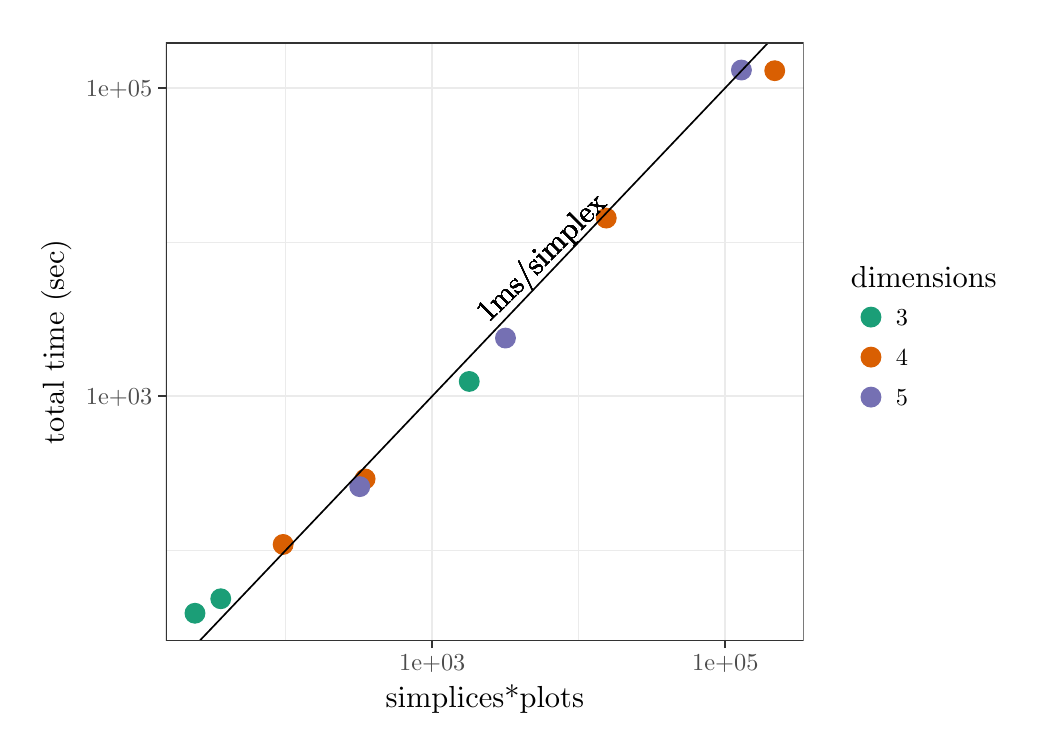
\begin{tikzpicture}[x=1pt,y=1pt]
\definecolor{fillColor}{RGB}{255,255,255}
\path[use as bounding box,fill=fillColor,fill opacity=0.00] (0,0) rectangle (361.35,252.94);
\begin{scope}
\path[clip] (  0.00,  0.00) rectangle (361.35,252.94);
\definecolor{drawColor}{RGB}{255,255,255}
\definecolor{fillColor}{RGB}{255,255,255}

\path[draw=drawColor,line width= 0.6pt,line join=round,line cap=round,fill=fillColor] (  0.00, -0.00) rectangle (361.35,252.94);
\end{scope}
\begin{scope}
\path[clip] ( 49.98, 31.53) rectangle (280.42,247.45);
\definecolor{fillColor}{RGB}{255,255,255}

\path[fill=fillColor] ( 49.98, 31.53) rectangle (280.42,247.45);
\definecolor{drawColor}{gray}{0.92}

\path[draw=drawColor,line width= 0.3pt,line join=round] ( 49.98, 64.13) --
	(280.42, 64.13);

\path[draw=drawColor,line width= 0.3pt,line join=round] ( 49.98,175.51) --
	(280.42,175.51);

\path[draw=drawColor,line width= 0.3pt,line join=round] ( 93.26, 31.53) --
	( 93.26,247.45);

\path[draw=drawColor,line width= 0.3pt,line join=round] (199.14, 31.53) --
	(199.14,247.45);

\path[draw=drawColor,line width= 0.6pt,line join=round] ( 49.98,119.82) --
	(280.42,119.82);

\path[draw=drawColor,line width= 0.6pt,line join=round] ( 49.98,231.20) --
	(280.42,231.20);

\path[draw=drawColor,line width= 0.6pt,line join=round] (146.20, 31.53) --
	(146.20,247.45);

\path[draw=drawColor,line width= 0.6pt,line join=round] (252.08, 31.53) --
	(252.08,247.45);
\definecolor{drawColor}{RGB}{27,158,119}
\definecolor{fillColor}{RGB}{27,158,119}

\path[draw=drawColor,line width= 0.4pt,line join=round,line cap=round,fill=fillColor] ( 69.77, 46.58) circle (  3.57);

\path[draw=drawColor,line width= 0.4pt,line join=round,line cap=round,fill=fillColor] ( 60.45, 41.34) circle (  3.57);
\definecolor{drawColor}{RGB}{217,95,2}
\definecolor{fillColor}{RGB}{217,95,2}

\path[draw=drawColor,line width= 0.4pt,line join=round,line cap=round,fill=fillColor] (121.93, 89.87) circle (  3.57);

\path[draw=drawColor,line width= 0.4pt,line join=round,line cap=round,fill=fillColor] ( 92.32, 66.20) circle (  3.57);
\definecolor{drawColor}{RGB}{117,112,179}
\definecolor{fillColor}{RGB}{117,112,179}

\path[draw=drawColor,line width= 0.4pt,line join=round,line cap=round,fill=fillColor] (172.65,140.78) circle (  3.57);

\path[draw=drawColor,line width= 0.4pt,line join=round,line cap=round,fill=fillColor] (120.00, 87.10) circle (  3.57);
\definecolor{drawColor}{RGB}{217,95,2}
\definecolor{fillColor}{RGB}{217,95,2}

\path[draw=drawColor,line width= 0.4pt,line join=round,line cap=round,fill=fillColor] (269.95,237.39) circle (  3.57);
\definecolor{drawColor}{RGB}{27,158,119}
\definecolor{fillColor}{RGB}{27,158,119}

\path[draw=drawColor,line width= 0.4pt,line join=round,line cap=round,fill=fillColor] (159.56,125.10) circle (  3.57);
\definecolor{drawColor}{RGB}{217,95,2}
\definecolor{fillColor}{RGB}{217,95,2}

\path[draw=drawColor,line width= 0.4pt,line join=round,line cap=round,fill=fillColor] (209.07,184.13) circle (  3.57);
\definecolor{drawColor}{RGB}{117,112,179}
\definecolor{fillColor}{RGB}{117,112,179}

\path[draw=drawColor,line width= 0.4pt,line join=round,line cap=round,fill=fillColor] (257.91,237.63) circle (  3.57);
\definecolor{drawColor}{RGB}{0,0,0}

\path[draw=drawColor,line width= 0.6pt,line join=round] ( 49.98, 18.59) -- (272.75,252.94);

\node[text=drawColor,rotate= 45.00,anchor=base,inner sep=0pt, outer sep=0pt, scale=  1.10] at (188.08,167.42) {1ms/simplex};

\node[text=drawColor,rotate= 45.00,anchor=base,inner sep=0pt, outer sep=0pt, scale=  1.10] at (188.08,167.42) {1ms/simplex};

\node[text=drawColor,rotate= 45.00,anchor=base,inner sep=0pt, outer sep=0pt, scale=  1.10] at (188.08,167.42) {1ms/simplex};

\node[text=drawColor,rotate= 45.00,anchor=base,inner sep=0pt, outer sep=0pt, scale=  1.10] at (188.08,167.42) {1ms/simplex};

\node[text=drawColor,rotate= 45.00,anchor=base,inner sep=0pt, outer sep=0pt, scale=  1.10] at (188.08,167.42) {1ms/simplex};

\node[text=drawColor,rotate= 45.00,anchor=base,inner sep=0pt, outer sep=0pt, scale=  1.10] at (188.08,167.42) {1ms/simplex};

\node[text=drawColor,rotate= 45.00,anchor=base,inner sep=0pt, outer sep=0pt, scale=  1.10] at (188.08,167.42) {1ms/simplex};

\node[text=drawColor,rotate= 45.00,anchor=base,inner sep=0pt, outer sep=0pt, scale=  1.10] at (188.08,167.42) {1ms/simplex};

\node[text=drawColor,rotate= 45.00,anchor=base,inner sep=0pt, outer sep=0pt, scale=  1.10] at (188.08,167.42) {1ms/simplex};

\node[text=drawColor,rotate= 45.00,anchor=base,inner sep=0pt, outer sep=0pt, scale=  1.10] at (188.08,167.42) {1ms/simplex};
\definecolor{drawColor}{gray}{0.20}

\path[draw=drawColor,line width= 0.6pt,line join=round,line cap=round] ( 49.98, 31.53) rectangle (280.42,247.45);
\end{scope}
\begin{scope}
\path[clip] (  0.00,  0.00) rectangle (361.35,252.94);
\definecolor{drawColor}{gray}{0.30}

\node[text=drawColor,anchor=base east,inner sep=0pt, outer sep=0pt, scale=  0.88] at ( 45.03,116.79) {1e+03};

\node[text=drawColor,anchor=base east,inner sep=0pt, outer sep=0pt, scale=  0.88] at ( 45.03,228.17) {1e+05};
\end{scope}
\begin{scope}
\path[clip] (  0.00,  0.00) rectangle (361.35,252.94);
\definecolor{drawColor}{gray}{0.20}

\path[draw=drawColor,line width= 0.6pt,line join=round] ( 47.23,119.82) --
	( 49.98,119.82);

\path[draw=drawColor,line width= 0.6pt,line join=round] ( 47.23,231.20) --
	( 49.98,231.20);
\end{scope}
\begin{scope}
\path[clip] (  0.00,  0.00) rectangle (361.35,252.94);
\definecolor{drawColor}{gray}{0.20}

\path[draw=drawColor,line width= 0.6pt,line join=round] (146.20, 28.78) --
	(146.20, 31.53);

\path[draw=drawColor,line width= 0.6pt,line join=round] (252.08, 28.78) --
	(252.08, 31.53);
\end{scope}
\begin{scope}
\path[clip] (  0.00,  0.00) rectangle (361.35,252.94);
\definecolor{drawColor}{gray}{0.30}

\node[text=drawColor,anchor=base,inner sep=0pt, outer sep=0pt, scale=  0.88] at (146.20, 20.52) {1e+03};

\node[text=drawColor,anchor=base,inner sep=0pt, outer sep=0pt, scale=  0.88] at (252.08, 20.52) {1e+05};
\end{scope}
\begin{scope}
\path[clip] (  0.00,  0.00) rectangle (361.35,252.94);
\definecolor{drawColor}{RGB}{0,0,0}

\node[text=drawColor,anchor=base,inner sep=0pt, outer sep=0pt, scale=  1.10] at (165.20,  7.44) {simplices*plots};
\end{scope}
\begin{scope}
\path[clip] (  0.00,  0.00) rectangle (361.35,252.94);
\definecolor{drawColor}{RGB}{0,0,0}

\node[text=drawColor,rotate= 90.00,anchor=base,inner sep=0pt, outer sep=0pt, scale=  1.10] at ( 13.08,139.49) {total time (sec)};
\end{scope}
\begin{scope}
\path[clip] (  0.00,  0.00) rectangle (361.35,252.94);
\definecolor{fillColor}{RGB}{255,255,255}

\path[fill=fillColor] (291.80,106.52) rectangle (355.85,172.45);
\end{scope}
\begin{scope}
\path[clip] (  0.00,  0.00) rectangle (361.35,252.94);
\definecolor{drawColor}{RGB}{0,0,0}

\node[text=drawColor,anchor=base west,inner sep=0pt, outer sep=0pt, scale=  1.10] at (297.49,159.19) {dimensions};
\end{scope}
\begin{scope}
\path[clip] (  0.00,  0.00) rectangle (361.35,252.94);
\definecolor{fillColor}{RGB}{255,255,255}

\path[fill=fillColor] (297.49,141.12) rectangle (311.95,155.57);
\end{scope}
\begin{scope}
\path[clip] (  0.00,  0.00) rectangle (361.35,252.94);
\definecolor{drawColor}{RGB}{27,158,119}
\definecolor{fillColor}{RGB}{27,158,119}

\path[draw=drawColor,line width= 0.4pt,line join=round,line cap=round,fill=fillColor] (304.72,148.35) circle (  3.57);
\end{scope}
\begin{scope}
\path[clip] (  0.00,  0.00) rectangle (361.35,252.94);
\definecolor{fillColor}{RGB}{255,255,255}

\path[fill=fillColor] (297.49,126.67) rectangle (311.95,141.12);
\end{scope}
\begin{scope}
\path[clip] (  0.00,  0.00) rectangle (361.35,252.94);
\definecolor{drawColor}{RGB}{217,95,2}
\definecolor{fillColor}{RGB}{217,95,2}

\path[draw=drawColor,line width= 0.4pt,line join=round,line cap=round,fill=fillColor] (304.72,133.89) circle (  3.57);
\end{scope}
\begin{scope}
\path[clip] (  0.00,  0.00) rectangle (361.35,252.94);
\definecolor{fillColor}{RGB}{255,255,255}

\path[fill=fillColor] (297.49,112.21) rectangle (311.95,126.67);
\end{scope}
\begin{scope}
\path[clip] (  0.00,  0.00) rectangle (361.35,252.94);
\definecolor{drawColor}{RGB}{117,112,179}
\definecolor{fillColor}{RGB}{117,112,179}

\path[draw=drawColor,line width= 0.4pt,line join=round,line cap=round,fill=fillColor] (304.72,119.44) circle (  3.57);
\end{scope}
\begin{scope}
\path[clip] (  0.00,  0.00) rectangle (361.35,252.94);
\definecolor{drawColor}{RGB}{0,0,0}

\node[text=drawColor,anchor=base west,inner sep=0pt, outer sep=0pt, scale=  0.88] at (313.75,145.32) {3};
\end{scope}
\begin{scope}
\path[clip] (  0.00,  0.00) rectangle (361.35,252.94);
\definecolor{drawColor}{RGB}{0,0,0}

\node[text=drawColor,anchor=base west,inner sep=0pt, outer sep=0pt, scale=  0.88] at (313.75,130.86) {4};
\end{scope}
\begin{scope}
\path[clip] (  0.00,  0.00) rectangle (361.35,252.94);
\definecolor{drawColor}{RGB}{0,0,0}

\node[text=drawColor,anchor=base west,inner sep=0pt, outer sep=0pt, scale=  0.88] at (313.75,116.41) {5};
\end{scope}
\end{tikzpicture}

  }
  \caption{%
    Chart showing the number of slicing operations 
    (simplices $\times$ number of plots) versus timing results from running 
    our algorithm on a number of different datasets. The axes are on a log-log
    scale. The points are all clustered around the ``1 ms/simplex'' line 
    showing that the running time is roughly one millisecond per slicing 
    operation.
  }
  \label{fig:timing}
\end{figure}

In order to test the running time of the slicing algorithm I ran a number of
experiments to understand the timing. I tested regular polytopes in 3, 4, and
5 dimensions as well as hyperspheres. I also tested the four-dimensional
version of the Klein bottle because it has a large number of simplices in its
mesh. For each test, I ran the slicing algorithm for all pairs of dimensions
and for $1,000$ focus points. I recorded the total wall clock time as well as
the number of simplices given by the quickhull algorithm. The testing machine
has an 8-core 3.2GHz Intel i7-6900K with 64GB of RAM.

The results are shown in \autoref{tbl:timings}. The total number of slicing
checks (\autoref{alg:slicing:single}) is the number of simplices, times the
number of pairs of dimensions ($d \choose 2$), times the total number of focus
points ($1,000$). I divide the total time by this number to show the time per
simplex. 

As we can see, the times are roughly constant between the number of
dimensions and simplices (see \autoref{fig:timing}). The reason the Klein 
bottle is faster is because
many slices do not hit any simplices and the algorithm will exit early
once this is detected. Right now this algorithm is not optimized.
For example, it would be greatly beneficial to pre-compute a spatial data
structure so that only slices that are likely to intersect simplices are
evaluated. Currently, the algorithm must check every simplex against every
focus point for every pair of dimensions. This is a lot of extra work for figures
such as the Klein bottle with many simplexes.



Understanding multi-dimensional spaces is difficult. Visualization can give
us context to help understand the geometry. With the direct visualization
of these multi-dimensional continuous datasets through slice views, we can
use a familiar concept to give context and meaning to a complex task.

Multi-dimensional continuous functions are commonly visualized with 2D slices
or topological views. With Sliceplorer, I explore 1D slices as an alternative
approach to show such functions. My goal with 1D slices is to combine the
benefits of topological views, that is, screen space efficiency, with those of
slices, that is a close resemblance of the underlying function.  I compare 1D
slices to 2D slices and topological views, first, by looking at their
performance with respect to common function analysis tasks. I also demonstrate
3 usage scenarios: the 2D sinc function, neural network regression, and
optimization traces. Based on this evaluation, I characterize the advantages
and drawbacks of each of these approaches, and show how interaction can be used
to overcome some of the shortcomings. 


I also presented Hypersliceplorer, an algorithm for generating 2D
slices of multi-dimensional shapes defined by a simplical mesh.  Often, slices
are generated by using a parametric form and then constraining parameters to
view the slice. In this case, I developed an algorithm to slice a simplical
mesh of any number of dimensions with a two-dimensional slice. In order to get
a global appreciation of the multi-dimensional object, I show multiple slices
by sampling a number of different slicing points and projecting the slices into
a single view per dimension pair. These slices are shown in an interactive
viewer which can switch between a global view (all slices) and a local view
(single slice). I show how this method can be used to study regular polytopes,
differences between spaces of polynomials, and multi-objective optimization
surfaces. 


Finally, I develop a method for predicting the rendering time to display
multi-dimensional data for the analysis of computer simulations using the
HyperSlice~\cite{Wijk:1993} method with Gaussian process model reconstruction.
My method relies on a theoretical understanding of how the data points are
drawn on slices and then fits the formula to a user's machine using practical
experiments.  I also describe the typical characteristics of data when
analyzing deterministic computer simulations as described by the statistics
community.  I then show the advantage of carefully considering how many data
points can be drawn in real time by proposing two approaches of how this
predictive formula can be used in a real-world system.


\subsection{Future}

My work has had a major focus on using direct visualization techniques to
understand multi-dimensional continuous spaces. My intention is that this work
can be expanded upon to herald in a new era of multi-dimensional data analysis.
In my opinion, the major innovations preventing this technique from being used
in a broader application are a library for slicing multi-dimensional spaces and
more user-focused projects.  Building on these two thrusts will move
multi-dimensional continuous data analysis to the mainstream.

One of the reasons for the lack of adoption for slice-based visualization of
multi-dimensional objects is the complete lack of software to generate even
static slice views. There are many libraries for popular data analysis
languages like Python, Javascript, and R. In order to make slice based views
more viable I plan to develop an interactive slice-based visualization software
based on the prototype tools I have already developed. This will lower the cost
of entry of slice-based views of multi-dimensional continuous datasets. The end
result is more users familiar with this visualization type.

In addition, more focused projects with end-users in the form of design
studies~\cite{Sedlmair:2012} will help to develop both the task taxonomy and
the visualization techniques. As part of the task abstraction, we can learn how
these users' tasks fit in with the task and data taxonomy proposed in this
thesis. Then we can refine and extend the task and data taxonomy. This taxonomy
will allow visualization researchers to identify gaps and develop tools to
address them, thus creating more effective visualizations of multi-dimensional
continuous data.


\subsection{Implications}

The main goal of my thesis was to explore what is possible with slice-based
visualizations of continuous multi-dimensional datasets. My hope is that this
work will serve as a basis for an increasing focus on direct visualization of
multi-dimensional objects. Often it seems that the default analysis technique
for more than three dimensions is to reduce
the dimensionality of the
data and then render the reduced data on screen. This suffers from issues of
distortion of distances and relative sizes. The analysis tasks for
multi-dimensional data are all developed around understanding the carefully
chosen dimensions. Hence, transforming these dimensions takes away a lot of
contextual knowledge about the simulation. 

I also hope to bring more attention to continuous multi-dimensional data analysis.
In the visualization community, most of the work on multi-dimensional and high-dimensional
data has focused on the discrete case. There are many task taxonomies, techniques,
and applications for discrete data. My hope with this thesis is that by developing
a task and data taxonomy as well as an in-depth study of direct visualization
techniques will bring similar attention to multi-dimensional continuous data
analysis. There are a number of under-explored application areas in this
field. I have identified some in my own work, but with further research in this
field will bring more knowledge and understanding about how we, as three-dimensional
beings can understand multi-dimensional continuous datasets.









\chapter{Fast slicing}
\label{chp:rendering}

%\chapter{Predicting the interactive rendering time threshold of Gaussian process models with HyperSlice}


\section{Motivation}

Many scientific studies investigate the relationship between
several explanatory variables (inputs) and one or more system response
variables (outputs), thereby leading to multi-dimensional data sets.  Such data
can arise in exploration of the input-output map for applications ranging from
weather, physics and biological processes to image segmentation systems.  
In these cases, the output
is actually a complex object such as a segmented image or 3D+time weather data.
A key step towards learning about the mechanisms that are present in a
computational model or laws that govern natural phenomena is to study how
changes in the input variables affect the output.  Visual inspection of
individual outputs is suitable in small multiples, but does not scale well with
increasing numbers of parameters, because of the large number of runs that are
required to adequately represent model behavior in the region of interest.  To
more comprehensively compare outputs, automation can be taken a step further,
for instance, by processing the outputs with feature extractors or fitness
functions that are relevant to the driving questions.  An interactive, visual
investigation of the resulting feature density distribution or fitness
landscape then becomes
possible~\cite{Feiner:1990,Muhlbacher:2013,Piringer:2010}, but is subject to 
some fundamental numerical
challenges that are topic of this chapter.

The general approach to
study deterministic computer models is known in the statistics community as
\emph{the design and analysis of computer experiments}~\cite{Santner:2003}.
This method involves reconstructing a continuous functional representation of
the relationships among variables of the system from a discrete set of 
samples and then investigating the
input/output relationship of the function.  Numerical methods for
this purpose include local derivative computation, global sensitivity
indices~\cite{Saltelli:2008}, and response surface
exploration~\cite{Box:2007}.  However, these derived computations have to be
set up carefully to yield meaningful results. 

The most well known example of non-interactive visualizations of the 
relationships is the scatterplot 
matrix for viewing discrete samples.
Another example are continuous plots of ``average'' behavior over the 
range of each
dimension, as exemplified in Chapman et al.~\cite{Chapman:1994}.
However, any 2D or 3D view of a multi-dimensional space necessarily requires
aggregation of that space.
We can only ``see'' a subsection of the parameter
space at one time.
Therefore, one must create multiple static views, each looking at 
the data from a different perspective.  A scatterplot matrix, for example,
shows a 2D projection of the data for each pair of dimensions.

By allowing for user interaction one is not limited to a
predetermined set of views.  
When the view selection changes then a new view of the data must be built
on the fly.
However, if the visualization system does not respond quickly to 
the user's interaction then the cognitive connection with the visualization
is lost~\cite{Shneiderman:1987} along with the advantage of adding 
interaction in the first place.
Arguments about what exact
response time makes a visualization \emph{interactive} vary.  However,
view updates somewhere between 10fps to 60fps are typically deemed acceptable.

One interactive, multi-dimensional, continuous
visualization method
is HyperSlice~\cite{Wijk:1993}, which presents the user
with a matrix of 2D slices of a multi-dimensional continuous function
around a particular viewpoint in space.
HyperSlice allows the user to change the
location of the viewpoint around which they are inspecting.
Given this method, it would be ideal to know if the number of
points or the dimensionality of the dataset will overwhelm the
graphics capabilities of the user's machine and slow the frame rate. 
Hence, we need a way to evaluate a priori what the frame rate will be
given some data. The main aim of this chapter is developing a methodology to 
estimate the rendering time of a multi-dimensional
visualization system in the form of a predictive formula.
We can even invert this formula so that, given a desired frame rate, 
we can compute the number of points 
possible to render in the given time.
This inversion can be used, for example, 
to automatically sub-sample the dataset when the predicted rendering 
time will be too slow.  

In order to be able to \emph{predict} the rendering time we need a
function for the average rendering time based on the size of the $N \times d$
multi-dimensional dataset as well as the search distance, $r$, over all possible view
points.  The advantage
of a predictive formula is that, once fit, one can estimate the rendering time
for all unknown values of $N$, $d$, and $r$.
In addition, we can use this function to examine the time and accuracy
trade-off in terms of point spread versus number of samples.

A proper prediction function should describe the number
of pixels that will need to be drawn based on the scene geometry.
Adapting this function
to each user's
hardware platform, requires a universal methodology that can be run on
each user's environment to make accurate predictions.
Combining this strong theoretical foundation with a fitting step makes our
method robust to further developments in GPU technology and algorithm 
development. One can simply recompute the time it takes the GPU to filter and
draw the points without having to worry about hardware-specific optimizations.

The contributions of this chapter are:

\begin{itemize}

\item An evaluation of how to render multi-dimensional slices on the GPU 
      and how one can use that to predict the number of pixels drawn on screen.

\item A fitting procedure for predicting rendering times on an
 individual user's hardware.

\item An application of the prediction formula where I show an algorithm
	  for subsampling data until I can render interactively.  I also 
	  show a UI dialog box for selecting the number of samples based on
	  the predicted rendering time.


\end{itemize}


\section{Related work}
\label{sec:related-work}

Multi-objective optimization and multi-dimensional objects are two areas
where it is important to study shapes in over three dimensions. We discuss 
these areas below. Topological techniques are based on viewing critical points
of manifolds~\cite{Correa:2011,Gerber:2010} or how contours merge and 
split~\cite{Carr:2003a}. We do not discuss them further. Manifold analysis
is very different than visualizing shapes. 

The need to understand multi-dimensional polytopes is apparent to 
geometers~\cite{Ziegler:2012}.
However, there are a number of cases in computational science where the
understanding of the size and the shape of a sub-section of the parameter space
is of importance~\cite{Bergner:2013,Sedlmair:2014}. One of these cases is
highlighted in \autoref{sec:bernstein}. Another use case is the study
of multi-dimensional Pareto fronts (\autoref{sec:pareto}).

\subsection{Multi-objective optimization}

In multi-objective optimization we have several scalar values that we wish to
optimize. The set of optimal points is known as the Pareto front.
If each objective measure is continuous then we have a continuous hull in one
orthant. We want to use this hull to analyze the trade-offs between objective
measures. Interactive decision maps~\cite{Lotov:2004} show a 3D Pareto front as
a series of 2D slices. Any objectives past three must be constrained to a value
however. Objective functions are difficult to sample since we often do
not have control over the sampling of the range of a function.  To
generate this hull one often samples the objective functions and then computes
the Pareto points using an algorithm such as NSGA-II~\cite{Deb:2002} or the
skyline algorithm~\cite{Borzsony:2001}. We can then generate the hull using
multi-dimensional marching cubes~\cite{Bhaniramka:2000}, the quickhull
algorithm~\cite{Barber:1996}, or alpha shapes~\cite{Edelsbrunner:1983}. These
can then be viewed in Hypersliceplorer as we do in \autoref{sec:pareto}.

An alternative is to treat the samples as a fixed set and then visualize the
relationship between possible combinations of objectives. Typically this is
done by examining the weight space through interaction. 
LineUp~\cite{Gratzl:2013} uses a ranked list approach and shows the user
how rankings will change as the user changes the relative weighting for each
objective. WeightLifter~\cite{Pajer:2016} extends this by also showing the
stability of rankings. The user can understand how much a particular objective
is affected by its weighting. This can help speed interactive exploration. 
Finally, the joint contour net~\cite{Carr:2014} can be used to compute how
often two objectives hold particular values simultaneously. 
In our case, the mental model is a continuous one. Thus it makes more sense
to show a continuous Pareto front.

\subsection{Multi-dimensional objects}

%TM: I wanted to add a sentence like this, but I dont think we need to after all: Since we are focusing on the visualization of continuous objects in multiple dimension, literature on projection based techniques is not relevant and will not be mentioned. 

%We review related work on the visualization of multi-dimensional continuous objects.

When speaking of 3D polytopes, their source is usually either from reconstruction of 3D point clouds 
(see Dey~\cite{Dey:2006})
or from iso-surfacing techniques (see Wenger~\cite{Wenger:2013}).
%However, we believe that the method of choice for visualization of 3D shapes are 3D renderings.
%Visualization of (continuous) objects in three (or fewer) dimensions is not that relevant for our discussion, since we believe that our method will not be of advantage here. Still, in the are of volume visualization there are quite a wealth of approaches for creating an iso-surface, which creates a 3D polytope. See also the excellent text books by Wenger or Day
%
%often falls under the name of
%volume visualization.  Three-dimensional volumes can be rendered using
%techniques isosurface techniques like marching cubes~\cite{Lorensen:1987a} or direct volume visualization. 
There are extensions to iso-surfacing techniques in multiple dimensions~\cite{Bhaniramka:2000}, 
%Marching cubes has been extended to arbitrary
%dimensions 
but in more than three dimensions we must distort the space somehow to visualize the object. 

For the visualization of 4D polytopes, there are a number of techniques for moving from four to three dimensions.  The
Schlegel diagram~\cite{Sommerville:1929} is one such method based on
projection. We pick a face of the figure, usually the largest, which is a
three-dimensional object. Then, all other faces are ``packed'' inside this face in
such a way that we can show the connections between faces. The Schlegel diagram
works well for regular polytopes where we have some previous intuition about
the faces. However, for an arbitrary simplical mesh, any face is a simplex
which we need to project into. All Schlegel diagrams of a simplical mesh look
like a simplex with a number of other simplices inside them. It can be
difficult to recover what the original object looks like because the
cross section is lost. An alternative approach is to treat the fourth dimension
as time and then produce an animation of the evolution of the shape in three
dimensions. In this case each frame of the animation is a 3D slice of the 
object. Rather than first projecting from 4D to 3D and then rendering the
projection, Hanson and Cross~\cite{Hanson:1993} propose a method to first
render the object in 4D and then view the three-dimensional projection. This
allows them to show unique lighting effects from the 4D surfaces.
%One can also use a stererographic projection. 
As with all projection methods, if the user is unaware of the details of the
method it can be difficult to build a mental model of the shape under study.

Hasse diagrams~\cite{Battista:1988} are based on showing the connectivity
between vertices of an object. These can be seen as network diagrams where the
vertices of the figure are the nodes in the graph and the edges of the graph
are the edges in the figure. These have a number of layout issues.  For visual
understanding, humans prefer a 2D planar graph~\cite{Kieffer:2016}. Good layouts
of the Hasse diagram must balance human aesthetic needs like few edge crossings
with the geometric interpretation. 
There are automatic layout
algorithms, such as the one by Battista et al.~\cite{Battista:1988}, but these
do not work in all cases.

For more than four dimensions, 
projection methods no longer work as well.  Techniques based on slicing the
space can be extended to any number of dimensions.  The techniques to perform
this so far, such as HyperSlice~\cite{Wijk:1993},
HyperMoVal~\cite{Piringer:2010}, and Sliceplorer~\cite{Torsney-Weir:2017a},
are designed to show slices of multi-dimensional manifolds.
They produce slices by
constraining all but two (for 2D slices) or one (for 1D slices) of the
dimensions to the focus point value and then producing a heatmap, contour plot,
or function plot. Sliceplorer addressed the focus point issue by sampling over
a number of focus points and projecting them down.  Exploded view
diagrams~\cite{Karpenko:2010} offer a hybrid method between a 3D volume
visualization and slicing.  However, they 
%also require a parametric description of the object under study and 
are limited to 3D objects. 
The global view of Hypersliceplorer is inspired by the idea of examining
cross sections. We also have a local
view which permits the user to look at a small number of self-selected slices.
We have developed a method to produce slices based on a simplical mesh which
is very useful given a discretized surface (see \autoref{fig:slicing}). 



\section{Problem description}

One method of studying the input/output relationship of computer simulations 
is known as the 
\emph{black-box model}. 
The black-box in this case refers to the simulation code itself.
The simulation code is complex and expensive to run
so direct analysis is difficult.
Under this analysis method one does not make any assumptions as to the
inner workings of the simulation code.  Instead, we model the simulator as an
unknown continuous function
that takes a number
of numerical inputs and produces a number of numerical outputs.  We know
the domain of the inputs.  We want to study how varying the inputs
affects the output. 

While we don't know anything about how the simulation works internally, we can  
sample it by selecting a particular input setting through the simulation 
and recording the outputs.  We can then use a continuous reconstruction
method built from a number of samples in order to estimate the 
\emph{response surface}.
This fitted continuous function
is known as an \emph{emulator} in the
statistics literature.  We can then study the input/output relationship
using the emulator instead.  

\subsection{1D analysis example}
\label{sec:1d_example}

A common choice in the statistics community for this emulator is known as the
Gaussian process model~\cite{Rasmussen:2006}.  
One advantage of the Gaussian process model is that the form is very well
known and easy to analyze.  
It also allows us to measure the uncertainty of the estimation.
In order to illustrate the 
advantages we will go through a 1D example here using a known function
$f(x) = \sin(x) + \cos(2x)$
as a stand-in for some simulation code.

We begin by taking a number of discrete samples of the function.  Ideally
we take as many as possible but this may be limited in terms of time or
budget.  Since we do not know anything about the behavior of the function 
in the region we are sampling,
we sample in some uniform random fashion.
The function as well as the sample locations are shown in 
\autoref{fig:reconstruction_sampling}.

\begin{figure}[htb]
  \centering
  {\tiny % Created by tikzDevice version 0.7.0 on 2014-07-31 11:04:19
% !TEX encoding = UTF-8 Unicode
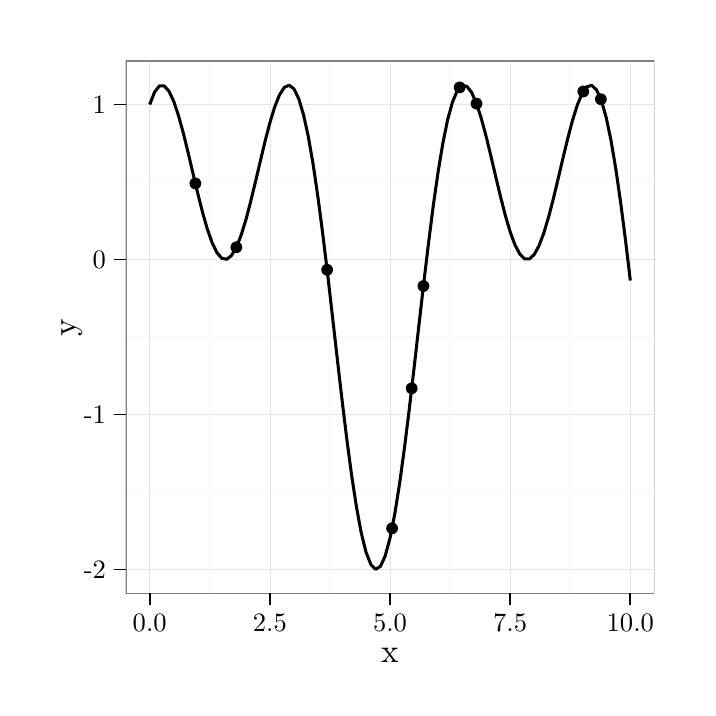
\begin{tikzpicture}[x=1pt,y=1pt]
\definecolor[named]{fillColor}{rgb}{1.00,1.00,1.00}
\path[use as bounding box,fill=fillColor,fill opacity=0.00] (0,0) rectangle (238.49,238.49);
\begin{scope}
\path[clip] (  0.00,  0.00) rectangle (238.49,238.49);
\definecolor[named]{drawColor}{rgb}{1.00,1.00,1.00}
\definecolor[named]{fillColor}{rgb}{1.00,1.00,1.00}

\path[draw=drawColor,line width= 0.6pt,line join=round,line cap=round,fill=fillColor] (  0.00,  0.00) rectangle (238.49,238.49);
\end{scope}
\begin{scope}
\path[clip] ( 35.42, 34.03) rectangle (226.45,226.45);
\definecolor[named]{fillColor}{rgb}{1.00,1.00,1.00}

\path[fill=fillColor] ( 35.42, 34.03) rectangle (226.45,226.45);
\definecolor[named]{drawColor}{rgb}{0.98,0.98,0.98}

\path[draw=drawColor,line width= 0.6pt,line join=round] ( 35.42, 70.75) --
	(226.45, 70.75);

\path[draw=drawColor,line width= 0.6pt,line join=round] ( 35.42,126.74) --
	(226.45,126.74);

\path[draw=drawColor,line width= 0.6pt,line join=round] ( 35.42,182.72) --
	(226.45,182.72);

\path[draw=drawColor,line width= 0.6pt,line join=round] ( 65.81, 34.03) --
	( 65.81,226.45);

\path[draw=drawColor,line width= 0.6pt,line join=round] (109.23, 34.03) --
	(109.23,226.45);

\path[draw=drawColor,line width= 0.6pt,line join=round] (152.64, 34.03) --
	(152.64,226.45);

\path[draw=drawColor,line width= 0.6pt,line join=round] (196.06, 34.03) --
	(196.06,226.45);
\definecolor[named]{drawColor}{rgb}{0.90,0.90,0.90}

\path[draw=drawColor,line width= 0.2pt,line join=round] ( 35.42, 42.76) --
	(226.45, 42.76);

\path[draw=drawColor,line width= 0.2pt,line join=round] ( 35.42, 98.74) --
	(226.45, 98.74);

\path[draw=drawColor,line width= 0.2pt,line join=round] ( 35.42,154.73) --
	(226.45,154.73);

\path[draw=drawColor,line width= 0.2pt,line join=round] ( 35.42,210.71) --
	(226.45,210.71);

\path[draw=drawColor,line width= 0.2pt,line join=round] ( 44.10, 34.03) --
	( 44.10,226.45);

\path[draw=drawColor,line width= 0.2pt,line join=round] ( 87.52, 34.03) --
	( 87.52,226.45);

\path[draw=drawColor,line width= 0.2pt,line join=round] (130.93, 34.03) --
	(130.93,226.45);

\path[draw=drawColor,line width= 0.2pt,line join=round] (174.35, 34.03) --
	(174.35,226.45);

\path[draw=drawColor,line width= 0.2pt,line join=round] (217.76, 34.03) --
	(217.76,226.45);
\definecolor[named]{drawColor}{rgb}{0.00,0.00,0.00}

\path[draw=drawColor,line width= 1.1pt,line join=round] ( 44.10,210.71) --
	( 45.84,215.19) --
	( 47.58,217.42) --
	( 49.31,217.48) --
	( 51.05,215.54) --
	( 52.79,211.82) --
	( 54.52,206.63) --
	( 56.26,200.31) --
	( 58.00,193.26) --
	( 59.73,185.86) --
	( 61.47,178.54) --
	( 63.21,171.68) --
	( 64.94,165.63) --
	( 66.68,160.70) --
	( 68.42,157.15) --
	( 70.15,155.15) --
	( 71.89,154.80) --
	( 73.63,156.12) --
	( 75.36,159.05) --
	( 77.10,163.43) --
	( 78.84,169.04) --
	( 80.57,175.61) --
	( 82.31,182.79) --
	( 84.05,190.20) --
	( 85.78,197.44) --
	( 87.52,204.12) --
	( 89.26,209.82) --
	( 90.99,214.19) --
	( 92.73,216.90) --
	( 94.47,217.70) --
	( 96.20,216.39) --
	( 97.94,212.85) --
	( 99.67,207.07) --
	(101.41,199.10) --
	(103.15,189.10) --
	(104.88,177.30) --
	(106.62,164.01) --
	(108.36,149.62) --
	(110.09,134.54) --
	(111.83,119.25) --
	(113.57,104.21) --
	(115.30, 89.93) --
	(117.04, 76.86) --
	(118.78, 65.44) --
	(120.51, 56.04) --
	(122.25, 48.99) --
	(123.99, 44.52) --
	(125.72, 42.78) --
	(127.46, 43.83) --
	(129.20, 47.64) --
	(130.93, 54.07) --
	(132.67, 62.91) --
	(134.41, 73.86) --
	(136.14, 86.56) --
	(137.88,100.59) --
	(139.62,115.48) --
	(141.35,130.75) --
	(143.09,145.93) --
	(144.83,160.53) --
	(146.56,174.13) --
	(148.30,186.33) --
	(150.04,196.80) --
	(151.77,205.29) --
	(153.51,211.62) --
	(155.25,215.72) --
	(156.98,217.58) --
	(158.72,217.29) --
	(160.46,215.03) --
	(162.19,211.04) --
	(163.93,205.63) --
	(165.67,199.17) --
	(167.40,192.03) --
	(169.14,184.62) --
	(170.88,177.34) --
	(172.61,170.59) --
	(174.35,164.71) --
	(176.08,160.00) --
	(177.82,156.70) --
	(179.56,154.97) --
	(181.29,154.91) --
	(183.03,156.50) --
	(184.77,159.69) --
	(186.50,164.29) --
	(188.24,170.09) --
	(189.98,176.78) --
	(191.71,184.03) --
	(193.45,191.44) --
	(195.19,198.62) --
	(196.92,205.15) --
	(198.66,210.66) --
	(200.40,214.77) --
	(202.13,217.18) --
	(203.87,217.63) --
	(205.61,215.95) --
	(207.34,212.03) --
	(209.08,205.88) --
	(210.82,197.55) --
	(212.55,187.23) --
	(214.29,175.16) --
	(216.03,161.66) --
	(217.76,147.12);
\definecolor[named]{fillColor}{rgb}{0.00,0.00,0.00}

\path[fill=fillColor] (207.13,212.64) circle (  2.13);

\path[fill=fillColor] (138.77,108.17) circle (  2.13);

\path[fill=fillColor] (162.19,211.04) circle (  2.13);

\path[fill=fillColor] (200.77,215.44) circle (  2.13);

\path[fill=fillColor] (143.00,145.13) circle (  2.13);

\path[fill=fillColor] (156.10,216.91) circle (  2.13);

\path[fill=fillColor] (131.68, 57.58) circle (  2.13);

\path[fill=fillColor] ( 75.41,159.14) circle (  2.13);

\path[fill=fillColor] ( 60.60,182.20) circle (  2.13);

\path[fill=fillColor] (108.20,151.00) circle (  2.13);
\definecolor[named]{drawColor}{rgb}{0.50,0.50,0.50}

\path[draw=drawColor,line width= 0.6pt,line join=round,line cap=round] ( 35.42, 34.03) rectangle (226.45,226.45);
\end{scope}
\begin{scope}
\path[clip] (  0.00,  0.00) rectangle (238.49,238.49);
\definecolor[named]{drawColor}{rgb}{0.00,0.00,0.00}

\node[text=drawColor,anchor=base east,inner sep=0pt, outer sep=0pt, scale=  0.96] at ( 28.31, 39.45) {-2};

\node[text=drawColor,anchor=base east,inner sep=0pt, outer sep=0pt, scale=  0.96] at ( 28.31, 95.44) {-1};

\node[text=drawColor,anchor=base east,inner sep=0pt, outer sep=0pt, scale=  0.96] at ( 28.31,151.42) {0};

\node[text=drawColor,anchor=base east,inner sep=0pt, outer sep=0pt, scale=  0.96] at ( 28.31,207.41) {1};
\end{scope}
\begin{scope}
\path[clip] (  0.00,  0.00) rectangle (238.49,238.49);
\definecolor[named]{drawColor}{rgb}{0.00,0.00,0.00}

\path[draw=drawColor,line width= 0.6pt,line join=round] ( 31.15, 42.76) --
	( 35.42, 42.76);

\path[draw=drawColor,line width= 0.6pt,line join=round] ( 31.15, 98.74) --
	( 35.42, 98.74);

\path[draw=drawColor,line width= 0.6pt,line join=round] ( 31.15,154.73) --
	( 35.42,154.73);

\path[draw=drawColor,line width= 0.6pt,line join=round] ( 31.15,210.71) --
	( 35.42,210.71);
\end{scope}
\begin{scope}
\path[clip] (  0.00,  0.00) rectangle (238.49,238.49);
\definecolor[named]{drawColor}{rgb}{0.00,0.00,0.00}

\path[draw=drawColor,line width= 0.6pt,line join=round] ( 44.10, 29.77) --
	( 44.10, 34.03);

\path[draw=drawColor,line width= 0.6pt,line join=round] ( 87.52, 29.77) --
	( 87.52, 34.03);

\path[draw=drawColor,line width= 0.6pt,line join=round] (130.93, 29.77) --
	(130.93, 34.03);

\path[draw=drawColor,line width= 0.6pt,line join=round] (174.35, 29.77) --
	(174.35, 34.03);

\path[draw=drawColor,line width= 0.6pt,line join=round] (217.76, 29.77) --
	(217.76, 34.03);
\end{scope}
\begin{scope}
\path[clip] (  0.00,  0.00) rectangle (238.49,238.49);
\definecolor[named]{drawColor}{rgb}{0.00,0.00,0.00}

\node[text=drawColor,anchor=base,inner sep=0pt, outer sep=0pt, scale=  0.96] at ( 44.10, 20.31) {0.0};

\node[text=drawColor,anchor=base,inner sep=0pt, outer sep=0pt, scale=  0.96] at ( 87.52, 20.31) {2.5};

\node[text=drawColor,anchor=base,inner sep=0pt, outer sep=0pt, scale=  0.96] at (130.93, 20.31) {5.0};

\node[text=drawColor,anchor=base,inner sep=0pt, outer sep=0pt, scale=  0.96] at (174.35, 20.31) {7.5};

\node[text=drawColor,anchor=base,inner sep=0pt, outer sep=0pt, scale=  0.96] at (217.76, 20.31) {10.0};
\end{scope}
\begin{scope}
\path[clip] (  0.00,  0.00) rectangle (238.49,238.49);
\definecolor[named]{drawColor}{rgb}{0.00,0.00,0.00}

\node[text=drawColor,anchor=base,inner sep=0pt, outer sep=0pt, scale=  1.20] at (130.93,  9.03) {x};
\end{scope}
\begin{scope}
\path[clip] (  0.00,  0.00) rectangle (238.49,238.49);
\definecolor[named]{drawColor}{rgb}{0.00,0.00,0.00}

\node[text=drawColor,rotate= 90.00,anchor=base,inner sep=0pt, outer sep=0pt, scale=  1.20] at ( 17.30,130.24) {y};
\end{scope}
\end{tikzpicture}
}
  \caption[The function $f(x) = sin(x) + cos(2x)$ uniformly sampled with 10 points]{%
    An example of taking 10 uniformly distributed samples of the function
    $f(x) = sin(x) + cos(2x)$.  The dots show the sampling locations.
  }
  \label{fig:reconstruction_sampling}
\end{figure}

We would prefer to take as many samples as possible in order to identify
the various peaks and valleys.
The interpolation method we choose depends on how we expect the values to
change between the sample points.
If we expect linear behavior then fitting a
piecewise linear function would be ideal.  If we expect more complex behavior
then we should fit higher-order functions.  I show 3 different fitting 
methods for the function in \autoref{fig:interp_methods}: piecewise linear (blue), 
cubic spline (green), and Gaussian process model (red) along with the true
function (black).  In this case the cubic spline and Gaussian process model
interpolations are very close to the true function, but the true function
normally would not be known beforehand.

\begin{figure}[htb]
  \centering
  {\tiny % Created by tikzDevice version 0.7.0 on 2014-07-31 11:04:27
% !TEX encoding = UTF-8 Unicode
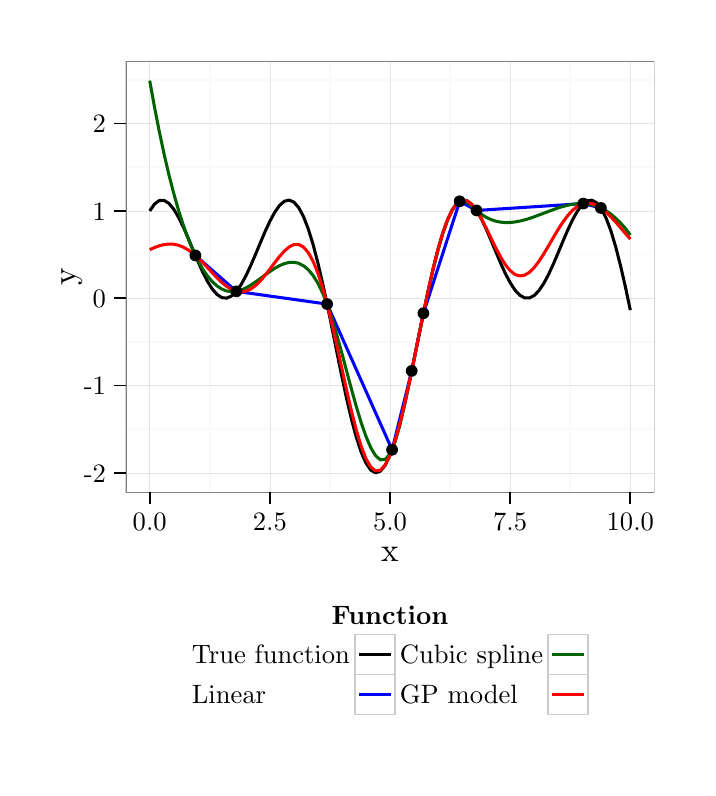
\begin{tikzpicture}[x=1pt,y=1pt]
\definecolor[named]{fillColor}{rgb}{1.00,1.00,1.00}
\path[use as bounding box,fill=fillColor,fill opacity=0.00] (0,0) rectangle (238.49,267.40);
\begin{scope}
\path[clip] (  0.00,  0.00) rectangle (238.49,267.40);
\definecolor[named]{drawColor}{rgb}{1.00,1.00,1.00}
\definecolor[named]{fillColor}{rgb}{1.00,1.00,1.00}

\path[draw=drawColor,line width= 0.6pt,line join=round,line cap=round,fill=fillColor] (  0.00,  0.00) rectangle (238.49,267.40);
\end{scope}
\begin{scope}
\path[clip] ( 35.42, 99.45) rectangle (226.45,255.35);
\definecolor[named]{fillColor}{rgb}{1.00,1.00,1.00}

\path[fill=fillColor] ( 35.42, 99.45) rectangle (226.45,255.35);
\definecolor[named]{drawColor}{rgb}{0.98,0.98,0.98}

\path[draw=drawColor,line width= 0.6pt,line join=round] ( 35.42,122.30) --
	(226.45,122.30);

\path[draw=drawColor,line width= 0.6pt,line join=round] ( 35.42,153.85) --
	(226.45,153.85);

\path[draw=drawColor,line width= 0.6pt,line join=round] ( 35.42,185.39) --
	(226.45,185.39);

\path[draw=drawColor,line width= 0.6pt,line join=round] ( 35.42,216.94) --
	(226.45,216.94);

\path[draw=drawColor,line width= 0.6pt,line join=round] ( 35.42,248.49) --
	(226.45,248.49);

\path[draw=drawColor,line width= 0.6pt,line join=round] ( 65.81, 99.45) --
	( 65.81,255.35);

\path[draw=drawColor,line width= 0.6pt,line join=round] (109.23, 99.45) --
	(109.23,255.35);

\path[draw=drawColor,line width= 0.6pt,line join=round] (152.64, 99.45) --
	(152.64,255.35);

\path[draw=drawColor,line width= 0.6pt,line join=round] (196.06, 99.45) --
	(196.06,255.35);
\definecolor[named]{drawColor}{rgb}{0.90,0.90,0.90}

\path[draw=drawColor,line width= 0.2pt,line join=round] ( 35.42,106.53) --
	(226.45,106.53);

\path[draw=drawColor,line width= 0.2pt,line join=round] ( 35.42,138.07) --
	(226.45,138.07);

\path[draw=drawColor,line width= 0.2pt,line join=round] ( 35.42,169.62) --
	(226.45,169.62);

\path[draw=drawColor,line width= 0.2pt,line join=round] ( 35.42,201.17) --
	(226.45,201.17);

\path[draw=drawColor,line width= 0.2pt,line join=round] ( 35.42,232.71) --
	(226.45,232.71);

\path[draw=drawColor,line width= 0.2pt,line join=round] ( 44.10, 99.45) --
	( 44.10,255.35);

\path[draw=drawColor,line width= 0.2pt,line join=round] ( 87.52, 99.45) --
	( 87.52,255.35);

\path[draw=drawColor,line width= 0.2pt,line join=round] (130.93, 99.45) --
	(130.93,255.35);

\path[draw=drawColor,line width= 0.2pt,line join=round] (174.35, 99.45) --
	(174.35,255.35);

\path[draw=drawColor,line width= 0.2pt,line join=round] (217.76, 99.45) --
	(217.76,255.35);
\definecolor[named]{drawColor}{rgb}{0.00,0.00,0.00}

\path[draw=drawColor,line width= 1.1pt,line join=round] ( 44.10,201.17) --
	( 45.84,203.69) --
	( 47.58,204.94) --
	( 49.31,204.98) --
	( 51.05,203.88) --
	( 52.79,201.79) --
	( 54.52,198.86) --
	( 56.26,195.31) --
	( 58.00,191.33) --
	( 59.73,187.16) --
	( 61.47,183.04) --
	( 63.21,179.17) --
	( 64.94,175.76) --
	( 66.68,172.99) --
	( 68.42,170.98) --
	( 70.15,169.86) --
	( 71.89,169.66) --
	( 73.63,170.41) --
	( 75.36,172.05) --
	( 77.10,174.52) --
	( 78.84,177.69) --
	( 80.57,181.39) --
	( 82.31,185.43) --
	( 84.05,189.61) --
	( 85.78,193.69) --
	( 87.52,197.45) --
	( 89.26,200.66) --
	( 90.99,203.13) --
	( 92.73,204.66) --
	( 94.47,205.10) --
	( 96.20,204.36) --
	( 97.94,202.37) --
	( 99.67,199.11) --
	(101.41,194.62) --
	(103.15,188.99) --
	(104.88,182.34) --
	(106.62,174.85) --
	(108.36,166.74) --
	(110.09,158.25) --
	(111.83,149.63) --
	(113.57,141.16) --
	(115.30,133.11) --
	(117.04,125.74) --
	(118.78,119.31) --
	(120.51,114.01) --
	(122.25,110.04) --
	(123.99,107.52) --
	(125.72,106.54) --
	(127.46,107.13) --
	(129.20,109.28) --
	(130.93,112.90) --
	(132.67,117.88) --
	(134.41,124.05) --
	(136.14,131.21) --
	(137.88,139.11) --
	(139.62,147.50) --
	(141.35,156.11) --
	(143.09,164.66) --
	(144.83,172.89) --
	(146.56,180.55) --
	(148.30,187.43) --
	(150.04,193.33) --
	(151.77,198.11) --
	(153.51,201.68) --
	(155.25,203.99) --
	(156.98,205.03) --
	(158.72,204.87) --
	(160.46,203.60) --
	(162.19,201.35) --
	(163.93,198.30) --
	(165.67,194.66) --
	(167.40,190.64) --
	(169.14,186.46) --
	(170.88,182.36) --
	(172.61,178.56) --
	(174.35,175.25) --
	(176.08,172.59) --
	(177.82,170.73) --
	(179.56,169.76) --
	(181.29,169.72) --
	(183.03,170.62) --
	(184.77,172.41) --
	(186.50,175.01) --
	(188.24,178.28) --
	(189.98,182.05) --
	(191.71,186.13) --
	(193.45,190.31) --
	(195.19,194.35) --
	(196.92,198.03) --
	(198.66,201.14) --
	(200.40,203.45) --
	(202.13,204.81) --
	(203.87,205.06) --
	(205.61,204.12) --
	(207.34,201.91) --
	(209.08,198.44) --
	(210.82,193.75) --
	(212.55,187.93) --
	(214.29,181.13) --
	(216.03,173.53) --
	(217.76,165.33);
\definecolor[named]{drawColor}{rgb}{0.00,0.00,1.00}

\path[draw=drawColor,line width= 1.1pt,line join=round] ( 60.60,185.10) --
	( 75.41,172.11) --
	(108.20,167.52) --
	(131.68,114.88) --
	(138.77,143.38) --
	(143.00,164.21) --
	(156.10,204.66) --
	(162.19,201.35) --
	(200.77,203.83) --
	(207.13,202.25);
\definecolor[named]{drawColor}{rgb}{0.00,0.39,0.00}

\path[draw=drawColor,line width= 1.1pt,line join=round] ( 44.10,248.27) --
	( 45.84,238.63) --
	( 47.58,229.76) --
	( 49.31,221.63) --
	( 51.05,214.20) --
	( 52.79,207.47) --
	( 54.52,201.40) --
	( 56.26,195.98) --
	( 58.00,191.18) --
	( 59.73,186.97) --
	( 61.47,183.34) --
	( 63.21,180.25) --
	( 64.94,177.70) --
	( 66.68,175.64) --
	( 68.42,174.07) --
	( 70.15,172.95) --
	( 71.89,172.26) --
	( 73.63,171.99) --
	( 75.36,172.10) --
	( 77.10,172.57) --
	( 78.84,173.33) --
	( 80.57,174.33) --
	( 82.31,175.49) --
	( 84.05,176.74) --
	( 85.78,178.03) --
	( 87.52,179.28) --
	( 89.26,180.42) --
	( 90.99,181.40) --
	( 92.73,182.13) --
	( 94.47,182.57) --
	( 96.20,182.63) --
	( 97.94,182.25) --
	( 99.67,181.38) --
	(101.41,179.92) --
	(103.15,177.83) --
	(104.88,175.04) --
	(106.62,171.47) --
	(108.36,167.07) --
	(110.09,161.82) --
	(111.83,155.93) --
	(113.57,149.61) --
	(115.30,143.10) --
	(117.04,136.62) --
	(118.78,130.40) --
	(120.51,124.68) --
	(122.25,119.67) --
	(123.99,115.61) --
	(125.72,112.73) --
	(127.46,111.24) --
	(129.20,111.39) --
	(130.93,113.39) --
	(132.67,117.46) --
	(134.41,123.42) --
	(136.14,130.76) --
	(137.88,138.98) --
	(139.62,147.58) --
	(141.35,156.20) --
	(143.09,164.65) --
	(144.83,172.74) --
	(146.56,180.30) --
	(148.30,187.14) --
	(150.04,193.11) --
	(151.77,198.04) --
	(153.51,201.75) --
	(155.25,204.07) --
	(156.98,204.86) --
	(158.72,204.31) --
	(160.46,202.95) --
	(162.19,201.35) --
	(163.93,199.97) --
	(165.67,198.88) --
	(167.40,198.05) --
	(169.14,197.48) --
	(170.88,197.12) --
	(172.61,196.97) --
	(174.35,197.00) --
	(176.08,197.19) --
	(177.82,197.51) --
	(179.56,197.94) --
	(181.29,198.46) --
	(183.03,199.06) --
	(184.77,199.70) --
	(186.50,200.36) --
	(188.24,201.02) --
	(189.98,201.67) --
	(191.71,202.27) --
	(193.45,202.80) --
	(195.19,203.25) --
	(196.92,203.59) --
	(198.66,203.79) --
	(200.40,203.84) --
	(202.13,203.72) --
	(203.87,203.40) --
	(205.61,202.88) --
	(207.34,202.15) --
	(209.08,201.18) --
	(210.82,199.97) --
	(212.55,198.51) --
	(214.29,196.78) --
	(216.03,194.78) --
	(217.76,192.47);
\definecolor[named]{drawColor}{rgb}{1.00,0.00,0.00}

\path[draw=drawColor,line width= 1.1pt,line join=round] ( 44.10,187.19) --
	( 45.84,187.96) --
	( 47.58,188.58) --
	( 49.31,189.02) --
	( 51.05,189.21) --
	( 52.79,189.14) --
	( 54.52,188.77) --
	( 56.26,188.09) --
	( 58.00,187.10) --
	( 59.73,185.83) --
	( 61.47,184.30) --
	( 63.21,182.58) --
	( 64.94,180.74) --
	( 66.68,178.86) --
	( 68.42,177.03) --
	( 70.15,175.35) --
	( 71.89,173.92) --
	( 73.63,172.81) --
	( 75.36,172.12) --
	( 77.10,171.89) --
	( 78.84,172.16) --
	( 80.57,172.94) --
	( 82.31,174.19) --
	( 84.05,175.87) --
	( 85.78,177.89) --
	( 87.52,180.14) --
	( 89.26,182.46) --
	( 90.99,184.69) --
	( 92.73,186.66) --
	( 94.47,188.16) --
	( 96.20,189.02) --
	( 97.94,189.05) --
	( 99.67,188.12) --
	(101.41,186.11) --
	(103.15,182.96) --
	(104.88,178.65) --
	(106.62,173.26) --
	(108.36,166.89) --
	(110.09,159.73) --
	(111.83,152.03) --
	(113.57,144.07) --
	(115.30,136.18) --
	(117.04,128.67) --
	(118.78,121.89) --
	(120.51,116.13) --
	(122.25,111.64) --
	(123.99,108.64) --
	(125.72,107.24) --
	(127.46,107.51) --
	(129.20,109.43) --
	(130.93,112.93) --
	(132.67,117.86) --
	(134.41,124.02) --
	(136.14,131.19) --
	(137.88,139.11) --
	(139.62,147.51) --
	(141.35,156.12) --
	(143.09,164.66) --
	(144.83,172.88) --
	(146.56,180.54) --
	(148.30,187.42) --
	(150.04,193.33) --
	(151.77,198.13) --
	(153.51,201.70) --
	(155.25,204.00) --
	(156.98,205.02) --
	(158.72,204.84) --
	(160.46,203.56) --
	(162.19,201.35) --
	(163.93,198.43) --
	(165.67,195.03) --
	(167.40,191.42) --
	(169.14,187.85) --
	(170.88,184.56) --
	(172.61,181.76) --
	(174.35,179.61) --
	(176.08,178.23) --
	(177.82,177.68) --
	(179.56,177.95) --
	(181.29,179.00) --
	(183.03,180.73) --
	(184.77,183.01) --
	(186.50,185.70) --
	(188.24,188.62) --
	(189.98,191.62) --
	(191.71,194.53) --
	(193.45,197.21) --
	(195.19,199.55) --
	(196.92,201.45) --
	(198.66,202.85) --
	(200.40,203.72) --
	(202.13,204.04) --
	(203.87,203.85) --
	(205.61,203.18) --
	(207.34,202.10) --
	(209.08,200.66) --
	(210.82,198.95) --
	(212.55,197.06) --
	(214.29,195.05) --
	(216.03,193.00) --
	(217.76,190.98);
\definecolor[named]{fillColor}{rgb}{0.00,0.00,0.00}

\path[fill=fillColor] (207.13,202.25) circle (  2.13);

\path[fill=fillColor] (138.77,143.38) circle (  2.13);

\path[fill=fillColor] (162.19,201.35) circle (  2.13);

\path[fill=fillColor] (200.77,203.83) circle (  2.13);

\path[fill=fillColor] (143.00,164.21) circle (  2.13);

\path[fill=fillColor] (156.10,204.66) circle (  2.13);

\path[fill=fillColor] (131.68,114.88) circle (  2.13);

\path[fill=fillColor] ( 75.41,172.11) circle (  2.13);

\path[fill=fillColor] ( 60.60,185.10) circle (  2.13);

\path[fill=fillColor] (108.20,167.52) circle (  2.13);
\definecolor[named]{drawColor}{rgb}{0.50,0.50,0.50}

\path[draw=drawColor,line width= 0.6pt,line join=round,line cap=round] ( 35.42, 99.45) rectangle (226.45,255.35);
\end{scope}
\begin{scope}
\path[clip] (  0.00,  0.00) rectangle (238.49,267.40);
\definecolor[named]{drawColor}{rgb}{0.00,0.00,0.00}

\node[text=drawColor,anchor=base east,inner sep=0pt, outer sep=0pt, scale=  0.96] at ( 28.31,103.22) {-2};

\node[text=drawColor,anchor=base east,inner sep=0pt, outer sep=0pt, scale=  0.96] at ( 28.31,134.77) {-1};

\node[text=drawColor,anchor=base east,inner sep=0pt, outer sep=0pt, scale=  0.96] at ( 28.31,166.31) {0};

\node[text=drawColor,anchor=base east,inner sep=0pt, outer sep=0pt, scale=  0.96] at ( 28.31,197.86) {1};

\node[text=drawColor,anchor=base east,inner sep=0pt, outer sep=0pt, scale=  0.96] at ( 28.31,229.41) {2};
\end{scope}
\begin{scope}
\path[clip] (  0.00,  0.00) rectangle (238.49,267.40);
\definecolor[named]{drawColor}{rgb}{0.00,0.00,0.00}

\path[draw=drawColor,line width= 0.6pt,line join=round] ( 31.15,106.53) --
	( 35.42,106.53);

\path[draw=drawColor,line width= 0.6pt,line join=round] ( 31.15,138.07) --
	( 35.42,138.07);

\path[draw=drawColor,line width= 0.6pt,line join=round] ( 31.15,169.62) --
	( 35.42,169.62);

\path[draw=drawColor,line width= 0.6pt,line join=round] ( 31.15,201.17) --
	( 35.42,201.17);

\path[draw=drawColor,line width= 0.6pt,line join=round] ( 31.15,232.71) --
	( 35.42,232.71);
\end{scope}
\begin{scope}
\path[clip] (  0.00,  0.00) rectangle (238.49,267.40);
\definecolor[named]{drawColor}{rgb}{0.00,0.00,0.00}

\path[draw=drawColor,line width= 0.6pt,line join=round] ( 44.10, 95.18) --
	( 44.10, 99.45);

\path[draw=drawColor,line width= 0.6pt,line join=round] ( 87.52, 95.18) --
	( 87.52, 99.45);

\path[draw=drawColor,line width= 0.6pt,line join=round] (130.93, 95.18) --
	(130.93, 99.45);

\path[draw=drawColor,line width= 0.6pt,line join=round] (174.35, 95.18) --
	(174.35, 99.45);

\path[draw=drawColor,line width= 0.6pt,line join=round] (217.76, 95.18) --
	(217.76, 99.45);
\end{scope}
\begin{scope}
\path[clip] (  0.00,  0.00) rectangle (238.49,267.40);
\definecolor[named]{drawColor}{rgb}{0.00,0.00,0.00}

\node[text=drawColor,anchor=base,inner sep=0pt, outer sep=0pt, scale=  0.96] at ( 44.10, 85.73) {0.0};

\node[text=drawColor,anchor=base,inner sep=0pt, outer sep=0pt, scale=  0.96] at ( 87.52, 85.73) {2.5};

\node[text=drawColor,anchor=base,inner sep=0pt, outer sep=0pt, scale=  0.96] at (130.93, 85.73) {5.0};

\node[text=drawColor,anchor=base,inner sep=0pt, outer sep=0pt, scale=  0.96] at (174.35, 85.73) {7.5};

\node[text=drawColor,anchor=base,inner sep=0pt, outer sep=0pt, scale=  0.96] at (217.76, 85.73) {10.0};
\end{scope}
\begin{scope}
\path[clip] (  0.00,  0.00) rectangle (238.49,267.40);
\definecolor[named]{drawColor}{rgb}{0.00,0.00,0.00}

\node[text=drawColor,anchor=base,inner sep=0pt, outer sep=0pt, scale=  1.20] at (130.93, 74.45) {x};
\end{scope}
\begin{scope}
\path[clip] (  0.00,  0.00) rectangle (238.49,267.40);
\definecolor[named]{drawColor}{rgb}{0.00,0.00,0.00}

\node[text=drawColor,rotate= 90.00,anchor=base,inner sep=0pt, outer sep=0pt, scale=  1.20] at ( 17.30,177.40) {y};
\end{scope}
\begin{scope}
\path[clip] (  0.00,  0.00) rectangle (238.49,267.40);
\definecolor[named]{fillColor}{rgb}{1.00,1.00,1.00}

\path[fill=fillColor] ( 55.07, 14.89) rectangle (206.79, 62.57);
\end{scope}
\begin{scope}
\path[clip] (  0.00,  0.00) rectangle (238.49,267.40);
\definecolor[named]{drawColor}{rgb}{0.00,0.00,0.00}

\node[text=drawColor,anchor=base,inner sep=0pt, outer sep=0pt, scale=  0.96] at (130.93, 51.68) {\bfseries Function};
\end{scope}
\begin{scope}
\path[clip] (  0.00,  0.00) rectangle (238.49,267.40);
\definecolor[named]{drawColor}{rgb}{0.80,0.80,0.80}
\definecolor[named]{fillColor}{rgb}{1.00,1.00,1.00}

\path[draw=drawColor,line width= 0.6pt,line join=round,line cap=round,fill=fillColor] (118.23, 33.61) rectangle (132.68, 48.07);
\end{scope}
\begin{scope}
\path[clip] (  0.00,  0.00) rectangle (238.49,267.40);
\definecolor[named]{drawColor}{rgb}{0.00,0.00,0.00}

\path[draw=drawColor,line width= 1.1pt,line join=round] (119.67, 40.84) -- (131.24, 40.84);
\end{scope}
\begin{scope}
\path[clip] (  0.00,  0.00) rectangle (238.49,267.40);
\definecolor[named]{drawColor}{rgb}{0.00,0.00,0.00}

\path[draw=drawColor,line width= 1.1pt,line join=round] (119.67, 40.84) -- (131.24, 40.84);
\end{scope}
\begin{scope}
\path[clip] (  0.00,  0.00) rectangle (238.49,267.40);
\definecolor[named]{drawColor}{rgb}{0.00,0.00,0.00}

\path[draw=drawColor,line width= 1.1pt,line join=round] (119.67, 40.84) -- (131.24, 40.84);
\end{scope}
\begin{scope}
\path[clip] (  0.00,  0.00) rectangle (238.49,267.40);
\definecolor[named]{drawColor}{rgb}{0.00,0.00,0.00}

\path[draw=drawColor,line width= 1.1pt,line join=round] (119.67, 40.84) -- (131.24, 40.84);
\end{scope}
\begin{scope}
\path[clip] (  0.00,  0.00) rectangle (238.49,267.40);
\definecolor[named]{drawColor}{rgb}{0.80,0.80,0.80}
\definecolor[named]{fillColor}{rgb}{1.00,1.00,1.00}

\path[draw=drawColor,line width= 0.6pt,line join=round,line cap=round,fill=fillColor] (118.23, 19.16) rectangle (132.68, 33.61);
\end{scope}
\begin{scope}
\path[clip] (  0.00,  0.00) rectangle (238.49,267.40);
\definecolor[named]{drawColor}{rgb}{0.00,0.00,1.00}

\path[draw=drawColor,line width= 1.1pt,line join=round] (119.67, 26.39) -- (131.24, 26.39);
\end{scope}
\begin{scope}
\path[clip] (  0.00,  0.00) rectangle (238.49,267.40);
\definecolor[named]{drawColor}{rgb}{0.00,0.00,1.00}

\path[draw=drawColor,line width= 1.1pt,line join=round] (119.67, 26.39) -- (131.24, 26.39);
\end{scope}
\begin{scope}
\path[clip] (  0.00,  0.00) rectangle (238.49,267.40);
\definecolor[named]{drawColor}{rgb}{0.00,0.00,1.00}

\path[draw=drawColor,line width= 1.1pt,line join=round] (119.67, 26.39) -- (131.24, 26.39);
\end{scope}
\begin{scope}
\path[clip] (  0.00,  0.00) rectangle (238.49,267.40);
\definecolor[named]{drawColor}{rgb}{0.00,0.00,1.00}

\path[draw=drawColor,line width= 1.1pt,line join=round] (119.67, 26.39) -- (131.24, 26.39);
\end{scope}
\begin{scope}
\path[clip] (  0.00,  0.00) rectangle (238.49,267.40);
\definecolor[named]{drawColor}{rgb}{0.80,0.80,0.80}
\definecolor[named]{fillColor}{rgb}{1.00,1.00,1.00}

\path[draw=drawColor,line width= 0.6pt,line join=round,line cap=round,fill=fillColor] (188.07, 33.61) rectangle (202.52, 48.07);
\end{scope}
\begin{scope}
\path[clip] (  0.00,  0.00) rectangle (238.49,267.40);
\definecolor[named]{drawColor}{rgb}{0.00,0.39,0.00}

\path[draw=drawColor,line width= 1.1pt,line join=round] (189.52, 40.84) -- (201.08, 40.84);
\end{scope}
\begin{scope}
\path[clip] (  0.00,  0.00) rectangle (238.49,267.40);
\definecolor[named]{drawColor}{rgb}{0.00,0.39,0.00}

\path[draw=drawColor,line width= 1.1pt,line join=round] (189.52, 40.84) -- (201.08, 40.84);
\end{scope}
\begin{scope}
\path[clip] (  0.00,  0.00) rectangle (238.49,267.40);
\definecolor[named]{drawColor}{rgb}{0.00,0.39,0.00}

\path[draw=drawColor,line width= 1.1pt,line join=round] (189.52, 40.84) -- (201.08, 40.84);
\end{scope}
\begin{scope}
\path[clip] (  0.00,  0.00) rectangle (238.49,267.40);
\definecolor[named]{drawColor}{rgb}{0.00,0.39,0.00}

\path[draw=drawColor,line width= 1.1pt,line join=round] (189.52, 40.84) -- (201.08, 40.84);
\end{scope}
\begin{scope}
\path[clip] (  0.00,  0.00) rectangle (238.49,267.40);
\definecolor[named]{drawColor}{rgb}{0.80,0.80,0.80}
\definecolor[named]{fillColor}{rgb}{1.00,1.00,1.00}

\path[draw=drawColor,line width= 0.6pt,line join=round,line cap=round,fill=fillColor] (188.07, 19.16) rectangle (202.52, 33.61);
\end{scope}
\begin{scope}
\path[clip] (  0.00,  0.00) rectangle (238.49,267.40);
\definecolor[named]{drawColor}{rgb}{1.00,0.00,0.00}

\path[draw=drawColor,line width= 1.1pt,line join=round] (189.52, 26.39) -- (201.08, 26.39);
\end{scope}
\begin{scope}
\path[clip] (  0.00,  0.00) rectangle (238.49,267.40);
\definecolor[named]{drawColor}{rgb}{1.00,0.00,0.00}

\path[draw=drawColor,line width= 1.1pt,line join=round] (189.52, 26.39) -- (201.08, 26.39);
\end{scope}
\begin{scope}
\path[clip] (  0.00,  0.00) rectangle (238.49,267.40);
\definecolor[named]{drawColor}{rgb}{1.00,0.00,0.00}

\path[draw=drawColor,line width= 1.1pt,line join=round] (189.52, 26.39) -- (201.08, 26.39);
\end{scope}
\begin{scope}
\path[clip] (  0.00,  0.00) rectangle (238.49,267.40);
\definecolor[named]{drawColor}{rgb}{1.00,0.00,0.00}

\path[draw=drawColor,line width= 1.1pt,line join=round] (189.52, 26.39) -- (201.08, 26.39);
\end{scope}
\begin{scope}
\path[clip] (  0.00,  0.00) rectangle (238.49,267.40);
\definecolor[named]{drawColor}{rgb}{0.00,0.00,0.00}

\node[text=drawColor,anchor=base west,inner sep=0pt, outer sep=0pt, scale=  0.96] at ( 59.34, 37.53) {True function};
\end{scope}
\begin{scope}
\path[clip] (  0.00,  0.00) rectangle (238.49,267.40);
\definecolor[named]{drawColor}{rgb}{0.00,0.00,0.00}

\node[text=drawColor,anchor=base west,inner sep=0pt, outer sep=0pt, scale=  0.96] at ( 59.34, 23.08) {Linear};
\end{scope}
\begin{scope}
\path[clip] (  0.00,  0.00) rectangle (238.49,267.40);
\definecolor[named]{drawColor}{rgb}{0.00,0.00,0.00}

\node[text=drawColor,anchor=base west,inner sep=0pt, outer sep=0pt, scale=  0.96] at (134.49, 37.53) {Cubic spline};
\end{scope}
\begin{scope}
\path[clip] (  0.00,  0.00) rectangle (238.49,267.40);
\definecolor[named]{drawColor}{rgb}{0.00,0.00,0.00}

\node[text=drawColor,anchor=base west,inner sep=0pt, outer sep=0pt, scale=  0.96] at (134.49, 23.08) {GP model};
\end{scope}
\end{tikzpicture}
}
  \caption[Example of different interpretation methods]{%
    Here, I show different interpolation methods of the function
    $f(x) = sin(x) + cos(2x)$ using the same 10 uniformly random distributed
    sample points.  I show the true function as well as piecewise linear,
    cubic spline, and Gaussian process interpolations.
  }
  \label{fig:interp_methods}
\end{figure}

The basic assumption of the Gaussian process model, however, is that the
function behavior between the sample points is random in the sense it could
take any path as long as it intersects the points and the correlation function
we select gives the general form of the function between the points.
The distribution of possible paths follows a multi-variate Gaussian
distribution through the selected sample points.  The mean of this 
distribution is the most likely path, which is typically what is visualized.
By modeling the behavior this way we also get a model for the uncertainty
at any point in the domain.  This uncertainty grows in proportion to the
distance to the sample points.  In \autoref{fig:gp_example} I show the Gaussian
process estimation of the above function given the sample points along with
the standard error of the estimation.  The error grows very quickly when
extrapolating, for example when $x < 1$.  This is 
because we are moving away from all sample points.  This is why in real 
applications it is important to sample near the edge of the domain.

\begin{figure}[htb]
  \centering
  {\tiny % Created by tikzDevice version 0.7.0 on 2014-07-31 11:04:32
% !TEX encoding = UTF-8 Unicode
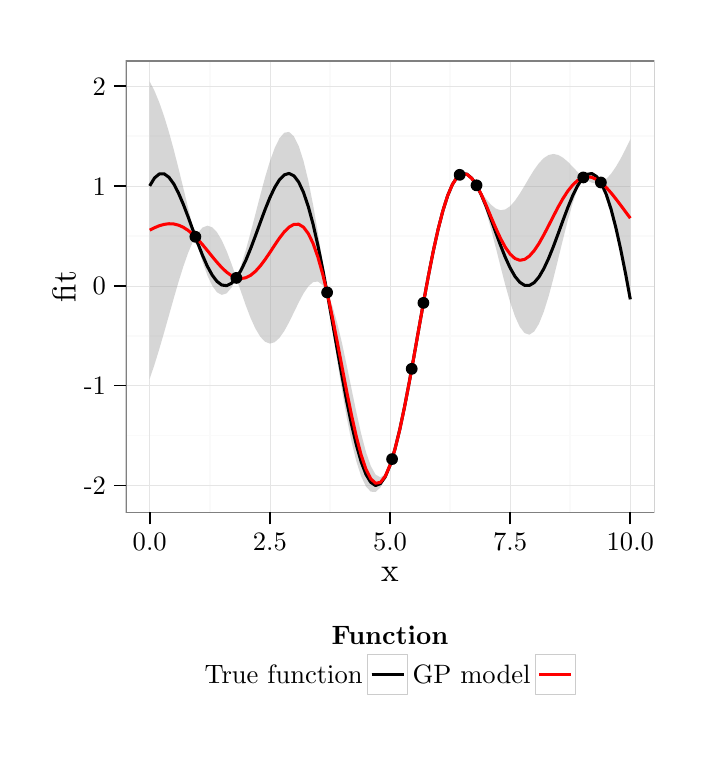
\begin{tikzpicture}[x=1pt,y=1pt]
\definecolor[named]{fillColor}{rgb}{1.00,1.00,1.00}
\path[use as bounding box,fill=fillColor,fill opacity=0.00] (0,0) rectangle (238.49,260.17);
\begin{scope}
\path[clip] (  0.00,  0.00) rectangle (238.49,260.17);
\definecolor[named]{drawColor}{rgb}{1.00,1.00,1.00}
\definecolor[named]{fillColor}{rgb}{1.00,1.00,1.00}

\path[draw=drawColor,line width= 0.6pt,line join=round,line cap=round,fill=fillColor] (  0.00,  0.00) rectangle (238.49,260.17);
\end{scope}
\begin{scope}
\path[clip] ( 35.42, 85.00) rectangle (226.45,248.13);
\definecolor[named]{fillColor}{rgb}{1.00,1.00,1.00}

\path[fill=fillColor] ( 35.42, 85.00) rectangle (226.45,248.13);
\definecolor[named]{drawColor}{rgb}{0.98,0.98,0.98}

\path[draw=drawColor,line width= 0.6pt,line join=round] ( 35.42,112.77) --
	(226.45,112.77);

\path[draw=drawColor,line width= 0.6pt,line join=round] ( 35.42,148.86) --
	(226.45,148.86);

\path[draw=drawColor,line width= 0.6pt,line join=round] ( 35.42,184.95) --
	(226.45,184.95);

\path[draw=drawColor,line width= 0.6pt,line join=round] ( 35.42,221.04) --
	(226.45,221.04);

\path[draw=drawColor,line width= 0.6pt,line join=round] ( 65.81, 85.00) --
	( 65.81,248.13);

\path[draw=drawColor,line width= 0.6pt,line join=round] (109.23, 85.00) --
	(109.23,248.13);

\path[draw=drawColor,line width= 0.6pt,line join=round] (152.64, 85.00) --
	(152.64,248.13);

\path[draw=drawColor,line width= 0.6pt,line join=round] (196.06, 85.00) --
	(196.06,248.13);
\definecolor[named]{drawColor}{rgb}{0.90,0.90,0.90}

\path[draw=drawColor,line width= 0.2pt,line join=round] ( 35.42, 94.72) --
	(226.45, 94.72);

\path[draw=drawColor,line width= 0.2pt,line join=round] ( 35.42,130.81) --
	(226.45,130.81);

\path[draw=drawColor,line width= 0.2pt,line join=round] ( 35.42,166.90) --
	(226.45,166.90);

\path[draw=drawColor,line width= 0.2pt,line join=round] ( 35.42,202.99) --
	(226.45,202.99);

\path[draw=drawColor,line width= 0.2pt,line join=round] ( 35.42,239.08) --
	(226.45,239.08);

\path[draw=drawColor,line width= 0.2pt,line join=round] ( 44.10, 85.00) --
	( 44.10,248.13);

\path[draw=drawColor,line width= 0.2pt,line join=round] ( 87.52, 85.00) --
	( 87.52,248.13);

\path[draw=drawColor,line width= 0.2pt,line join=round] (130.93, 85.00) --
	(130.93,248.13);

\path[draw=drawColor,line width= 0.2pt,line join=round] (174.35, 85.00) --
	(174.35,248.13);

\path[draw=drawColor,line width= 0.2pt,line join=round] (217.76, 85.00) --
	(217.76,248.13);
\definecolor[named]{fillColor}{rgb}{0.60,0.60,0.60}

\path[fill=fillColor,fill opacity=0.40] ( 44.10,240.71) --
	( 45.84,237.29) --
	( 47.58,233.08) --
	( 49.31,228.11) --
	( 51.05,222.40) --
	( 52.79,216.07) --
	( 54.52,209.25) --
	( 56.26,202.14) --
	( 58.00,194.95) --
	( 59.73,187.94) --
	( 61.47,186.02) --
	( 63.21,187.94) --
	( 64.94,188.62) --
	( 66.68,188.04) --
	( 68.42,186.23) --
	( 70.15,183.31) --
	( 71.89,179.45) --
	( 73.63,174.89) --
	( 75.36,169.89) --
	( 77.10,174.26) --
	( 78.84,179.86) --
	( 80.57,186.17) --
	( 82.31,192.87) --
	( 84.05,199.61) --
	( 85.78,206.06) --
	( 87.52,211.85) --
	( 89.26,216.67) --
	( 90.99,220.21) --
	( 92.73,222.21) --
	( 94.47,222.49) --
	( 96.20,220.90) --
	( 97.94,217.40) --
	( 99.67,212.00) --
	(101.41,204.84) --
	(103.15,196.09) --
	(104.88,186.04) --
	(106.62,175.01) --
	(108.36,164.15) --
	(110.09,159.57) --
	(111.83,153.51) --
	(113.57,146.23) --
	(115.30,138.09) --
	(117.04,129.57) --
	(118.78,121.16) --
	(120.51,113.41) --
	(122.25,106.80) --
	(123.99,101.77) --
	(125.72, 98.66) --
	(127.46, 97.67) --
	(129.20, 98.88) --
	(130.93,102.23) --
	(132.67,107.84) --
	(134.41,114.98) --
	(136.14,123.12) --
	(137.88,132.05) --
	(139.62,141.65) --
	(141.35,151.52) --
	(143.09,161.24) --
	(144.83,170.80) --
	(146.56,179.76) --
	(148.30,187.81) --
	(150.04,194.66) --
	(151.77,200.11) --
	(153.51,204.03) --
	(155.25,206.38) --
	(156.98,207.56) --
	(158.72,207.56) --
	(160.46,206.10) --
	(162.19,203.20) --
	(163.93,200.72) --
	(165.67,198.28) --
	(167.40,196.22) --
	(169.14,194.80) --
	(170.88,194.20) --
	(172.61,194.50) --
	(174.35,195.68) --
	(176.08,197.64) --
	(177.82,200.18) --
	(179.56,203.06) --
	(181.29,206.04) --
	(183.03,208.84) --
	(184.77,211.24) --
	(186.50,213.05) --
	(188.24,214.16) --
	(189.98,214.53) --
	(191.71,214.17) --
	(193.45,213.17) --
	(195.19,211.70) --
	(196.92,209.93) --
	(198.66,208.09) --
	(200.40,206.37) --
	(202.13,207.58) --
	(203.87,208.02) --
	(205.61,206.73) --
	(207.34,204.33) --
	(209.08,205.51) --
	(210.82,207.39) --
	(212.55,209.89) --
	(214.29,212.88) --
	(216.03,216.25) --
	(217.76,219.82) --
	(217.76,162.86) --
	(216.03,171.05) --
	(214.29,179.10) --
	(212.55,186.69) --
	(210.82,193.53) --
	(209.08,199.31) --
	(207.34,203.78) --
	(205.61,203.87) --
	(203.87,204.12) --
	(202.13,204.99) --
	(200.40,205.44) --
	(198.66,201.75) --
	(196.92,196.69) --
	(195.19,190.58) --
	(193.45,183.76) --
	(191.71,176.63) --
	(189.98,169.61) --
	(188.24,163.11) --
	(186.50,157.54) --
	(184.77,153.21) --
	(183.03,150.38) --
	(181.29,149.22) --
	(179.56,149.80) --
	(177.82,152.07) --
	(176.08,155.88) --
	(174.35,160.99) --
	(172.61,167.09) --
	(170.88,173.80) --
	(169.14,180.73) --
	(167.40,187.47) --
	(165.67,193.67) --
	(163.93,199.00) --
	(162.19,203.20) --
	(160.46,205.36) --
	(158.72,206.82) --
	(156.98,207.25) --
	(155.25,206.08) --
	(153.51,203.17) --
	(151.77,198.92) --
	(150.04,193.40) --
	(148.30,186.73) --
	(146.56,179.04) --
	(144.83,170.47) --
	(143.09,161.22) --
	(141.35,151.38) --
	(139.62,141.56) --
	(137.88,131.93) --
	(136.14,122.74) --
	(134.41,114.48) --
	(132.67,107.52) --
	(130.93,101.87) --
	(129.20, 97.21) --
	(127.46, 94.02) --
	(125.72, 92.41) --
	(123.99, 92.50) --
	(122.25, 94.35) --
	(120.51, 98.01) --
	(118.78,103.43) --
	(117.04,110.55) --
	(115.30,119.19) --
	(113.57,129.12) --
	(111.83,140.05) --
	(110.09,151.61) --
	(108.36,163.40) --
	(106.62,167.11) --
	(104.88,168.43) --
	(103.15,168.23) --
	(101.41,166.70) --
	( 99.67,164.14) --
	( 97.94,160.88) --
	( 96.20,157.29) --
	( 94.47,153.74) --
	( 92.73,150.57) --
	( 90.99,148.09) --
	( 89.26,146.51) --
	( 87.52,146.02) --
	( 85.78,146.68) --
	( 84.05,148.50) --
	( 82.31,151.40) --
	( 80.57,155.22) --
	( 78.84,159.75) --
	( 77.10,164.74) --
	( 75.36,169.64) --
	( 73.63,166.23) --
	( 71.89,164.18) --
	( 70.15,163.61) --
	( 68.42,164.53) --
	( 66.68,166.91) --
	( 64.94,170.63) --
	( 63.21,175.52) --
	( 61.47,181.38) --
	( 59.73,182.94) --
	( 58.00,178.85) --
	( 56.26,173.92) --
	( 54.52,168.36) --
	( 52.79,162.39) --
	( 51.05,156.23) --
	( 49.31,150.07) --
	( 47.58,144.11) --
	( 45.84,138.48) --
	( 44.10,133.29) --
	cycle;

\path[] ( 44.10,187.00) --
	( 45.84,187.88) --
	( 47.58,188.60) --
	( 49.31,189.09) --
	( 51.05,189.32) --
	( 52.79,189.23) --
	( 54.52,188.81) --
	( 56.26,188.03) --
	( 58.00,186.90) --
	( 59.73,185.44) --
	( 61.47,183.70) --
	( 63.21,181.73) --
	( 64.94,179.63) --
	( 66.68,177.47) --
	( 68.42,175.38) --
	( 70.15,173.46) --
	( 71.89,171.82) --
	( 73.63,170.56) --
	( 75.36,169.76) --
	( 77.10,169.50) --
	( 78.84,169.81) --
	( 80.57,170.69) --
	( 82.31,172.13) --
	( 84.05,174.06) --
	( 85.78,176.37) --
	( 87.52,178.93) --
	( 89.26,181.59) --
	( 90.99,184.15) --
	( 92.73,186.39) --
	( 94.47,188.11) --
	( 96.20,189.09) --
	( 97.94,189.14) --
	( 99.67,188.07) --
	(101.41,185.77) --
	(103.15,182.16) --
	(104.88,177.24) --
	(106.62,171.06) --
	(108.36,163.78) --
	(110.09,155.59) --
	(111.83,146.78) --
	(113.57,137.68) --
	(115.30,128.64) --
	(117.04,120.06) --
	(118.78,112.30) --
	(120.51,105.71) --
	(122.25,100.58) --
	(123.99, 97.14) --
	(125.72, 95.54) --
	(127.46, 95.85) --
	(129.20, 98.05) --
	(130.93,102.05) --
	(132.67,107.68) --
	(134.41,114.73) --
	(136.14,122.93) --
	(137.88,131.99) --
	(139.62,141.60) --
	(141.35,151.45) --
	(143.09,161.23) --
	(144.83,170.64) --
	(146.56,179.40) --
	(148.30,187.27) --
	(150.04,194.03) --
	(151.77,199.51) --
	(153.51,203.60) --
	(155.25,206.23) --
	(156.98,207.40) --
	(158.72,207.19) --
	(160.46,205.73) --
	(162.19,203.20) --
	(163.93,199.86) --
	(165.67,195.98) --
	(167.40,191.85) --
	(169.14,187.76) --
	(170.88,184.00) --
	(172.61,180.79) --
	(174.35,178.34) --
	(176.08,176.76) --
	(177.82,176.12) --
	(179.56,176.43) --
	(181.29,177.63) --
	(183.03,179.61) --
	(184.77,182.22) --
	(186.50,185.29) --
	(188.24,188.64) --
	(189.98,192.07) --
	(191.71,195.40) --
	(193.45,198.47) --
	(195.19,201.14) --
	(196.92,203.31) --
	(198.66,204.92) --
	(200.40,205.91) --
	(202.13,206.28) --
	(203.87,206.07) --
	(205.61,205.30) --
	(207.34,204.06) --
	(209.08,202.41) --
	(210.82,200.46) --
	(212.55,198.29) --
	(214.29,195.99) --
	(216.03,193.65) --
	(217.76,191.34);
\definecolor[named]{drawColor}{rgb}{0.00,0.00,0.00}

\path[draw=drawColor,line width= 1.1pt,line join=round] ( 44.10,202.99) --
	( 45.84,205.88) --
	( 47.58,207.32) --
	( 49.31,207.36) --
	( 51.05,206.10) --
	( 52.79,203.71) --
	( 54.52,200.36) --
	( 56.26,196.29) --
	( 58.00,191.74) --
	( 59.73,186.97) --
	( 61.47,182.25) --
	( 63.21,177.83) --
	( 64.94,173.93) --
	( 66.68,170.75) --
	( 68.42,168.46) --
	( 70.15,167.17) --
	( 71.89,166.95) --
	( 73.63,167.80) --
	( 75.36,169.69) --
	( 77.10,172.51) --
	( 78.84,176.13) --
	( 80.57,180.36) --
	( 82.31,184.99) --
	( 84.05,189.77) --
	( 85.78,194.44) --
	( 87.52,198.74) --
	( 89.26,202.42) --
	( 90.99,205.23) --
	( 92.73,206.98) --
	( 94.47,207.50) --
	( 96.20,206.65) --
	( 97.94,204.37) --
	( 99.67,200.64) --
	(101.41,195.50) --
	(103.15,189.06) --
	(104.88,181.45) --
	(106.62,172.89) --
	(108.36,163.61) --
	(110.09,153.89) --
	(111.83,144.03) --
	(113.57,134.34) --
	(115.30,125.13) --
	(117.04,116.71) --
	(118.78,109.34) --
	(120.51,103.29) --
	(122.25, 98.74) --
	(123.99, 95.86) --
	(125.72, 94.73) --
	(127.46, 95.41) --
	(129.20, 97.87) --
	(130.93,102.01) --
	(132.67,107.71) --
	(134.41,114.77) --
	(136.14,122.96) --
	(137.88,132.00) --
	(139.62,141.60) --
	(141.35,151.45) --
	(143.09,161.23) --
	(144.83,170.65) --
	(146.56,179.41) --
	(148.30,187.27) --
	(150.04,194.02) --
	(151.77,199.50) --
	(153.51,203.58) --
	(155.25,206.22) --
	(156.98,207.42) --
	(158.72,207.23) --
	(160.46,205.77) --
	(162.19,203.20) --
	(163.93,199.72) --
	(165.67,195.55) --
	(167.40,190.95) --
	(169.14,186.17) --
	(170.88,181.48) --
	(172.61,177.13) --
	(174.35,173.34) --
	(176.08,170.30) --
	(177.82,168.17) --
	(179.56,167.06) --
	(181.29,167.02) --
	(183.03,168.05) --
	(184.77,170.10) --
	(186.50,173.07) --
	(188.24,176.80) --
	(189.98,181.12) --
	(191.71,185.79) --
	(193.45,190.57) --
	(195.19,195.20) --
	(196.92,199.41) --
	(198.66,202.96) --
	(200.40,205.61) --
	(202.13,207.16) --
	(203.87,207.45) --
	(205.61,206.37) --
	(207.34,203.84) --
	(209.08,199.87) --
	(210.82,194.51) --
	(212.55,187.85) --
	(214.29,180.07) --
	(216.03,171.37) --
	(217.76,162.00);
\definecolor[named]{drawColor}{rgb}{1.00,0.00,0.00}

\path[draw=drawColor,line width= 1.1pt,line join=round] ( 44.10,187.00) --
	( 45.84,187.88) --
	( 47.58,188.60) --
	( 49.31,189.09) --
	( 51.05,189.32) --
	( 52.79,189.23) --
	( 54.52,188.81) --
	( 56.26,188.03) --
	( 58.00,186.90) --
	( 59.73,185.44) --
	( 61.47,183.70) --
	( 63.21,181.73) --
	( 64.94,179.63) --
	( 66.68,177.47) --
	( 68.42,175.38) --
	( 70.15,173.46) --
	( 71.89,171.82) --
	( 73.63,170.56) --
	( 75.36,169.76) --
	( 77.10,169.50) --
	( 78.84,169.81) --
	( 80.57,170.69) --
	( 82.31,172.13) --
	( 84.05,174.06) --
	( 85.78,176.37) --
	( 87.52,178.93) --
	( 89.26,181.59) --
	( 90.99,184.15) --
	( 92.73,186.39) --
	( 94.47,188.11) --
	( 96.20,189.09) --
	( 97.94,189.14) --
	( 99.67,188.07) --
	(101.41,185.77) --
	(103.15,182.16) --
	(104.88,177.24) --
	(106.62,171.06) --
	(108.36,163.78) --
	(110.09,155.59) --
	(111.83,146.78) --
	(113.57,137.68) --
	(115.30,128.64) --
	(117.04,120.06) --
	(118.78,112.30) --
	(120.51,105.71) --
	(122.25,100.58) --
	(123.99, 97.14) --
	(125.72, 95.54) --
	(127.46, 95.85) --
	(129.20, 98.05) --
	(130.93,102.05) --
	(132.67,107.68) --
	(134.41,114.73) --
	(136.14,122.93) --
	(137.88,131.99) --
	(139.62,141.60) --
	(141.35,151.45) --
	(143.09,161.23) --
	(144.83,170.64) --
	(146.56,179.40) --
	(148.30,187.27) --
	(150.04,194.03) --
	(151.77,199.51) --
	(153.51,203.60) --
	(155.25,206.23) --
	(156.98,207.40) --
	(158.72,207.19) --
	(160.46,205.73) --
	(162.19,203.20) --
	(163.93,199.86) --
	(165.67,195.98) --
	(167.40,191.85) --
	(169.14,187.76) --
	(170.88,184.00) --
	(172.61,180.79) --
	(174.35,178.34) --
	(176.08,176.76) --
	(177.82,176.12) --
	(179.56,176.43) --
	(181.29,177.63) --
	(183.03,179.61) --
	(184.77,182.22) --
	(186.50,185.29) --
	(188.24,188.64) --
	(189.98,192.07) --
	(191.71,195.40) --
	(193.45,198.47) --
	(195.19,201.14) --
	(196.92,203.31) --
	(198.66,204.92) --
	(200.40,205.91) --
	(202.13,206.28) --
	(203.87,206.07) --
	(205.61,205.30) --
	(207.34,204.06) --
	(209.08,202.41) --
	(210.82,200.46) --
	(212.55,198.29) --
	(214.29,195.99) --
	(216.03,193.65) --
	(217.76,191.34);
\definecolor[named]{fillColor}{rgb}{0.00,0.00,0.00}

\path[fill=fillColor] (207.13,204.23) circle (  2.13);

\path[fill=fillColor] (138.77,136.89) circle (  2.13);

\path[fill=fillColor] (162.19,203.20) circle (  2.13);

\path[fill=fillColor] (200.77,206.04) circle (  2.13);

\path[fill=fillColor] (143.00,160.72) circle (  2.13);

\path[fill=fillColor] (156.10,206.99) circle (  2.13);

\path[fill=fillColor] (131.68,104.28) circle (  2.13);

\path[fill=fillColor] ( 75.41,169.75) circle (  2.13);

\path[fill=fillColor] ( 60.60,184.61) circle (  2.13);

\path[fill=fillColor] (108.20,164.50) circle (  2.13);
\definecolor[named]{drawColor}{rgb}{0.50,0.50,0.50}

\path[draw=drawColor,line width= 0.6pt,line join=round,line cap=round] ( 35.42, 85.00) rectangle (226.45,248.13);
\end{scope}
\begin{scope}
\path[clip] (  0.00,  0.00) rectangle (238.49,260.17);
\definecolor[named]{drawColor}{rgb}{0.00,0.00,0.00}

\node[text=drawColor,anchor=base east,inner sep=0pt, outer sep=0pt, scale=  0.96] at ( 28.31, 91.42) {-2};

\node[text=drawColor,anchor=base east,inner sep=0pt, outer sep=0pt, scale=  0.96] at ( 28.31,127.51) {-1};

\node[text=drawColor,anchor=base east,inner sep=0pt, outer sep=0pt, scale=  0.96] at ( 28.31,163.60) {0};

\node[text=drawColor,anchor=base east,inner sep=0pt, outer sep=0pt, scale=  0.96] at ( 28.31,199.69) {1};

\node[text=drawColor,anchor=base east,inner sep=0pt, outer sep=0pt, scale=  0.96] at ( 28.31,235.78) {2};
\end{scope}
\begin{scope}
\path[clip] (  0.00,  0.00) rectangle (238.49,260.17);
\definecolor[named]{drawColor}{rgb}{0.00,0.00,0.00}

\path[draw=drawColor,line width= 0.6pt,line join=round] ( 31.15, 94.72) --
	( 35.42, 94.72);

\path[draw=drawColor,line width= 0.6pt,line join=round] ( 31.15,130.81) --
	( 35.42,130.81);

\path[draw=drawColor,line width= 0.6pt,line join=round] ( 31.15,166.90) --
	( 35.42,166.90);

\path[draw=drawColor,line width= 0.6pt,line join=round] ( 31.15,202.99) --
	( 35.42,202.99);

\path[draw=drawColor,line width= 0.6pt,line join=round] ( 31.15,239.08) --
	( 35.42,239.08);
\end{scope}
\begin{scope}
\path[clip] (  0.00,  0.00) rectangle (238.49,260.17);
\definecolor[named]{drawColor}{rgb}{0.00,0.00,0.00}

\path[draw=drawColor,line width= 0.6pt,line join=round] ( 44.10, 80.73) --
	( 44.10, 85.00);

\path[draw=drawColor,line width= 0.6pt,line join=round] ( 87.52, 80.73) --
	( 87.52, 85.00);

\path[draw=drawColor,line width= 0.6pt,line join=round] (130.93, 80.73) --
	(130.93, 85.00);

\path[draw=drawColor,line width= 0.6pt,line join=round] (174.35, 80.73) --
	(174.35, 85.00);

\path[draw=drawColor,line width= 0.6pt,line join=round] (217.76, 80.73) --
	(217.76, 85.00);
\end{scope}
\begin{scope}
\path[clip] (  0.00,  0.00) rectangle (238.49,260.17);
\definecolor[named]{drawColor}{rgb}{0.00,0.00,0.00}

\node[text=drawColor,anchor=base,inner sep=0pt, outer sep=0pt, scale=  0.96] at ( 44.10, 71.27) {0.0};

\node[text=drawColor,anchor=base,inner sep=0pt, outer sep=0pt, scale=  0.96] at ( 87.52, 71.27) {2.5};

\node[text=drawColor,anchor=base,inner sep=0pt, outer sep=0pt, scale=  0.96] at (130.93, 71.27) {5.0};

\node[text=drawColor,anchor=base,inner sep=0pt, outer sep=0pt, scale=  0.96] at (174.35, 71.27) {7.5};

\node[text=drawColor,anchor=base,inner sep=0pt, outer sep=0pt, scale=  0.96] at (217.76, 71.27) {10.0};
\end{scope}
\begin{scope}
\path[clip] (  0.00,  0.00) rectangle (238.49,260.17);
\definecolor[named]{drawColor}{rgb}{0.00,0.00,0.00}

\node[text=drawColor,anchor=base,inner sep=0pt, outer sep=0pt, scale=  1.20] at (130.93, 60.00) {x};
\end{scope}
\begin{scope}
\path[clip] (  0.00,  0.00) rectangle (238.49,260.17);
\definecolor[named]{drawColor}{rgb}{0.00,0.00,0.00}

\node[text=drawColor,rotate= 90.00,anchor=base,inner sep=0pt, outer sep=0pt, scale=  1.20] at ( 17.30,166.56) {fit};
\end{scope}
\begin{scope}
\path[clip] (  0.00,  0.00) rectangle (238.49,260.17);
\definecolor[named]{fillColor}{rgb}{1.00,1.00,1.00}

\path[fill=fillColor] ( 59.67, 14.89) rectangle (202.20, 48.12);
\end{scope}
\begin{scope}
\path[clip] (  0.00,  0.00) rectangle (238.49,260.17);
\definecolor[named]{drawColor}{rgb}{0.00,0.00,0.00}

\node[text=drawColor,anchor=base,inner sep=0pt, outer sep=0pt, scale=  0.96] at (130.93, 37.23) {\bfseries Function};
\end{scope}
\begin{scope}
\path[clip] (  0.00,  0.00) rectangle (238.49,260.17);
\definecolor[named]{drawColor}{rgb}{0.80,0.80,0.80}
\definecolor[named]{fillColor}{rgb}{1.00,1.00,1.00}

\path[draw=drawColor,line width= 0.6pt,line join=round,line cap=round,fill=fillColor] (122.82, 19.16) rectangle (137.28, 33.61);
\end{scope}
\begin{scope}
\path[clip] (  0.00,  0.00) rectangle (238.49,260.17);
\definecolor[named]{drawColor}{rgb}{0.00,0.00,0.00}

\path[draw=drawColor,line width= 1.1pt,line join=round] (124.27, 26.39) -- (135.83, 26.39);
\end{scope}
\begin{scope}
\path[clip] (  0.00,  0.00) rectangle (238.49,260.17);
\definecolor[named]{drawColor}{rgb}{0.00,0.00,0.00}

\path[draw=drawColor,line width= 1.1pt,line join=round] (124.27, 26.39) -- (135.83, 26.39);
\end{scope}
\begin{scope}
\path[clip] (  0.00,  0.00) rectangle (238.49,260.17);
\definecolor[named]{drawColor}{rgb}{0.80,0.80,0.80}
\definecolor[named]{fillColor}{rgb}{1.00,1.00,1.00}

\path[draw=drawColor,line width= 0.6pt,line join=round,line cap=round,fill=fillColor] (183.48, 19.16) rectangle (197.93, 33.61);
\end{scope}
\begin{scope}
\path[clip] (  0.00,  0.00) rectangle (238.49,260.17);
\definecolor[named]{drawColor}{rgb}{1.00,0.00,0.00}

\path[draw=drawColor,line width= 1.1pt,line join=round] (184.92, 26.39) -- (196.49, 26.39);
\end{scope}
\begin{scope}
\path[clip] (  0.00,  0.00) rectangle (238.49,260.17);
\definecolor[named]{drawColor}{rgb}{1.00,0.00,0.00}

\path[draw=drawColor,line width= 1.1pt,line join=round] (184.92, 26.39) -- (196.49, 26.39);
\end{scope}
\begin{scope}
\path[clip] (  0.00,  0.00) rectangle (238.49,260.17);
\definecolor[named]{drawColor}{rgb}{0.00,0.00,0.00}

\node[text=drawColor,anchor=base west,inner sep=0pt, outer sep=0pt, scale=  0.96] at ( 63.93, 23.08) {True function};
\end{scope}
\begin{scope}
\path[clip] (  0.00,  0.00) rectangle (238.49,260.17);
\definecolor[named]{drawColor}{rgb}{0.00,0.00,0.00}

\node[text=drawColor,anchor=base west,inner sep=0pt, outer sep=0pt, scale=  0.96] at (139.08, 23.08) {GP model};
\end{scope}
\end{tikzpicture}
}
  \caption[Gaussian process interpolation example]{%
    The Gaussian process interpolation of the function 
    $f(x) = sin(x) + cos(2x)$ from 10 uniformly distributed samples.  
    The standard error of estimation from the model is shown in gray.
    Note that the standard error increases with the distance from the sample
    points.
  }
  \label{fig:gp_example}
\end{figure}

Parameterizing a Gaussian process model means correctly parameterizing the 
correlation functions to the data samples.  If the function varies a lot 
between the sample points then we would expect low correlation between the
sample points, while if the function is relatively stable between the sample
points then we would expect high correlation between the points.  
In the spatial sense, this high and low correlation can be seen as the 
amount of influence the value of a particular sample point has on the value
at another location a particular distance away.

\subsection{Applications in multi-D}
\label{sec:gp_applications}

Gaussian process regression is very common in the statistics community
to analyze simulations among other types of data.
There exist a number of examples where Gaussian process regression along
with a uniformly distributed experimental design is used in order to 
run an analysis.
Using uniform sampling with a Gaussian process model 
has been applied in 
an optimization scenario, as with
Couckuyt et al.~\cite{Couckuyt:2010}.  They used a sparse initial sampling
and then built a GP model to emulate microwave filter and textile antenna
simulations.  They then incrementally ran additional samples of the simulation
in order to find optimal parameter settings.  This process of finding 
additional sample locations can be quite expensive computationally.
Hutter et al.~\cite{Hutter:2010}
develop a method to find new sample locations when under a time budget.
They then applied this method to find optimal parameters for a search
algorithm for a propositional satisfyability solver.
This method was also used to perform
a sensitivity analysis of an arctic sea ice
prediction model~\cite{Chapman:1994}.  They decomposed the Gaussian process
model to find ``average'' behavior due to each model parameter.
Linkletter et al.~\cite{Linkletter:2006} 
used Gaussian process models to measure the sensitivity of parameters to
a cylinder deformation simulation to reduce the parameter space from 14 input 
factors to seven.
Kaufman et al.~\cite{Kaufman:2011} use compactly supported correlation 
functions to build Gaussian process models efficiently on
very large data sets.  This was applied to cosmological data.
Hensman et al.~\cite{Hensman:2013} used an approach to train 
a Gaussian process model on $700,000$ data points in an $8$-dimensional space
to build a model to predict flight delays using a lower rank covariance
matrix.
Shepherd and Owenius~\cite{Shepherd:2012} used Gaussian process models 
as a classification tool in order to classify voxels in dPET images in order
to find tumor sites.

\begin{table}[htb]
\centering
\caption[A summary of the literature using Gaussian process models]{%
  A summary of the literature described in \autoref{sec:gp_applications}.  I
  show the domain of application of each paper, their analysis goal, as
  well as the number of samples and number of input parameters (dimensions)
  of the simulation used to train the GP model. 
}
\label{tb:literature}
\begin{adjustbox}{max width=\linewidth}
\begin{tabular}{|r|lrrl|}
  \hline
  Reference & Application & Dimensions & Samples & Goal \\
  \hline
  Couckuyt et al.~\cite{Couckuyt:2010} & Microwave filter & 5 & 51 & Optimization \\
  Couckuyt et al.~\cite{Couckuyt:2010} & Textile antenna & 2 & 14 & Optimization \\
  Hutter et al.~\cite{Hutter:2010} & Propositional logic satisfyability & 4 & 25 & Optimization \\
  Chapman et al.~\cite{Chapman:1994} & Sea ice prediction & 13 & 157 & Sensitivity analysis \\
  Linkletter et al.~\cite{Linkletter:2006} & Cylinder deformation model & 14 & 118 & Sensitivity analysis \\
  Kaufman et al.~\cite{Kaufman:2011} & Cosmological data  & 4 & 20,000 & Prediction \\
  Hensman et al.~\cite{Hensman:2013} & Flight delays & 8 & 700,000 & Prediction \\
  Shepherd and Owenius~\cite{Shepherd:2012} & dPET data in radiation oncology & 4 & 6 patient images & Classification \\
  \hline
\end{tabular}
\end{adjustbox}
\end{table}

As one can see, there are a wide variety of application domains.  However, 
all these analyses share commonalities.
I show the summary information of these studies in \autoref{tb:literature}.
The number of inputs is typically on
the order of 5--15 inputs. Each of these may correspond to a known factor that
can vary in the real world like wind speed or the velocity of a particle, or
an unknown fixed-quantity in the real world like Planck's constant or the
gravitational constant.  The simulation code typically creates a complex
object like a 3D+time model of the world or a segmented image. On these
outputs scientists define a number of feature extractors or objective
functions which reduce the complex output to a set of numerical 
attributes~\cite{Sedlmair:2014}.
Therefore, for each simulation run we get a vector of scalar input factors and
the corresponding vector of scalar outputs.  Each scalar output can be
considered in a separate analysis so in this chapter we assume that there is
only one scalar output for each input configuration.

The practical number of simulation samples range from a few hundred to hundreds
of thousands.  This is due to either time or monetary constraints.  Running more
simulations than this simply takes too long or costs too much.  
Based on these
data I test my timing function on dimensions $3$--$8$ and run up to 
$1,000,000$ sample points.


\subsection{Pipeline description}

Despite the wide variety of application areas, all the simulation studies 
mentioned follow a standard procedure for
analysis.
They start with a uniform sampling of the parameter space. This is
usually done with a space-filling
design like a Latin 
hypercube~\cite{Mckay:1979}, Halton
sequence~\cite{Halton:1964}, or Centroidal Voronoi tesselation~\cite{Du:1999}. 
Without any knowledge of the relative
importance of the dimensions they are sampled equally.

The
simulation is run using each sample and the outputs are recorded. If the
output is a complex object then feature
extractors are run on the outputs to generate scalar results.
Then, an emulator is built of this
process. Prediction using this emulator must be fast as we will want to
evaluate it at many points. Often, a Gaussian process
model~\cite{Rasmussen:2006} is selected for the emulator. 

\begin{figure}[htb]
  \centering
  \includegraphics[width=\linewidth]{tuner}
  \caption[Tuner's HyperSlice view]{\
    Screenshot of Tuner~\cite{Torsney-Weir:2011} demonstrating the
    HyperSlice~\cite{Wijk:1993} method for rendering an
    $8$-dimensional parameter space using squared exponential kernel 
    reconstruction on an image segmentation dataset.
    Here we show the view using the conditional mean of the Gaussian 
    process model.
  } 
  \label{fig:tuner}
\end{figure}

With this emulator the user can now analyze the input\slash output
relationship of the simulation. This can be done in a variety of ways, either by
looking at static plots~\cite{Chapman:1994} or by interactively exploring the
response surface~\cite{Torsney-Weir:2011}. We show an example of the
HyperSlice technique for interactively exploring the response surface
as implemented in Tuner~\cite{Torsney-Weir:2011} in \autoref{fig:tuner}.  
In this case we show the conditional mean of the Gaussian process model.
Tuner can also show the estimation variability if desired.

Interactive 
exploration of the Gaussian process model is a 
relatively new technique as it is more complex to implement and the limits
in terms of the number of points and how the size of the kernels affects 
interactivity is not yet understood.  
The rest of this chapter will discuss how to address both these questions.
I present a rendering algorithm which is similar to 
splatting~\cite{Mueller:1998}
to render the Gaussian
process prediction function using HyperSlice.
I also develop a method to determine when
the interactivity of the rendering will fail taking into account the geometric 
interpretation of the Gaussian process model as well as the performance
of an individual user's machine.


\section{Requirements}
\label{sec:requirements}

Sampling the Gaussian process prediction forumula \autoref{eq:gp-pred} directly in
sufficient density to draw the slices is expensive because each evaluation
requires computing the dot product of two size $N$ vectors.  Instead, we render
the prediction formula in order to exploit the inherent parallelism provided by
the GPU. Before describing the algorithm itself, we first need to consider
what the multi-dimensional ``scene'' we are trying to render looks like.  The
fundamental data type we are given are sample points of the simulation.  This
section describes how these sample points are transformed into higher-order
geometric primitives and then what happens when slicing them in order to be
drawn on screen.

\subsection{Scene geometry}
\label{sec:scene_geometry}

Here we will describe the spatial interpretation of the Gaussian process
model so that one can build an intuition for the geometric portion of the 
prediction formula.  This spatial interpretation is very close to the 
form used for the splatting algorithm.

The spatial interpretation of the Gaussian process model using squared 
exponential correlation is a set of 
multi-dimensional ellipsoids, one for each sample point. 
One may be tempted to think this is due to uncertainty at the sample points
but this is not the case here as the outputs of a computer simulation are
considered exact. The ellipsoids are due to giving the correlation functions
compact support.
In order to see
why this is the case we first begin by looking at the formula for the 
``best linear unbiased prediction,''
at an arbitrary location
in the parameter space, $x'$, which is,

\begin{align}
  \hat{y}(x') &= \mu + \vec{r}(x') R^{-1} (\vec{Y} - \mu)' \text{,}
  \label{eq:gp-pred}
\end{align}
here $\vec{r}$ is a vector of functions, one per sample point
and each element of $r$, $r_i$, is the correlation 
between
sample point $x_i$ and $x'$.  
$\vec{Y}$ is a vector of the sampled outputs.
$\mu$ is the estimated process mean.
$R$ is 
the $N \times N$ correlation matrix 
between the sample points using the same correlation function.
We also note that neither $R^{-1}$ nor $(Y - \mu)$
depend on $x'$ so we let the vector, 
$\vec{\Upsilon} = R^{-1} (\vec{Y} - \mu)'$.  
Then, we can write \autoref{eq:gp-pred} in a linear form,

\begin{align*}
  \hat{y}(x') &= \mu + r(x') \vec{\Upsilon} \\
              &= \mu + \sum_{i=1}^N r_i(x') \Upsilon_i \text{.}
\end{align*}
The value $\Upsilon_i$ is $f'(x_i)$ and $\hat{y}$ is $\hat{f}$ from 
\autoref{eq:kernel_regression} which is normalized by $R^{-1}$ from 
\autoref{eq:gp-pred}.

%This means that the prediction formula for the Gaussian process model 
%is essentially a kernel-based estimator. The shape of the kernels depends 
%on the chosen
%correlation function. In the case of Gaussian correlation, if we set a
%maximum distance at which points no longer have any effect, the kernels are
%ellipsoidal in shape. In our case, and as reported in section 
%\SC{sec:calibrationmethodology} this value is, $\epsilon = 1x10-9$.  
%The $\theta$
%parameters determine the size of the ellipses.  Increasing the value of a
%particular $\theta$ will cause the size of the kernel to decrease in that
%dimension.

A common choice for $r(\cdot)$ is the squared exponential correlation
function
which has infinite support and is strictly 
positive meaning that it is defined everywhere in the domain and always 
returns some positive value however small. 
There is a different falloff
parameter for each dimension.
For visualization purposes these small values don't contribute a
perceivable effect.
Therefore, we set a lower bound on the correlation value which we denote,
$\epsilon = 1 \times 10^{-9}$, essentially giving the correlation function
compact support. This can also be done using specific compactly supported 
correlation functions as in
Kaufman et al.~\cite{Kaufman:2011}. 
The squared exponential correlation function is radial meaning the
correlation amount between points decreases as the distance increases.
This $\epsilon$ value essentially creates a $d$-dimensional ellipsoid region
around each sample point with principal axis lengths related to the 
correlation falloff parameter. The sample point will only influence 
predictions within this region.

%Typically in modeling simulations the output values
%are considered deterministic. That is, for a given parameter configuration,
%the simulation will always yield the same output.
%A spatial-embedding of the Gaussian process model with 
%squared exponential correlation functions will yield $N$
%$d$-dimensional ellipsoids.  These ellipses may overlap or be clipped by the
%edges of the parameter space depending on location and size. However, they
%still have a known layout.  
%We can use this known layout to predict how this will influence the number
%of pixels we need to draw on screen.

\subsection{HyperSlice effect on scene geometry}
\label{sec:hypersliceeffectonscenegeometry}

The last step is using some method to examine this multi-dimensional
scene on a computer screen.  Our
chosen display method is the
HyperSlice~\cite{Wijk:1993} technique to which will draw $2$-dimensional
slices through these multi-dimensional ellipsoids on screen.  
HyperSlice relies on the user selecting a \textit{viewpoint} which 
determines the location in the multi-dimensional parameter space where to
position of the slices.
In \autoref{fig:hyperslice_geometry} we show the representation for the
HyperSlice technique in both 2 and 3 dimensions.  In 2D the slicing plane (what
one sees) is a line.  In 3D it is a 2D plane slicing through the space.  In 
higher dimensions it is also a 2D slicing plane.

\begin{figure}[htb]
  \centering
  \begin{subfigure}{0.25\textwidth}
    \centering
    \includegraphics[width=\textwidth]{gp_diagram_2d}
    \caption{2D view}
    \label{fig:hs_2d}
  \end{subfigure}%
  \begin{subfigure}{0.25\textwidth}
    \centering
    \includegraphics[width=\textwidth]{gp_diagram_3d}
    \caption{3D view}
    \label{fig:hs_3d}
  \end{subfigure}
  \caption[Example of 2D slices of 2D and 3D spheres]{
    Diagrams showing how the HyperSlice~\cite{Wijk:1993} method ``slices'' 
    through the 
    kernels of the Gaussian process model in both 2D (a) and 3D (b).  The 
    slicing plane is denoted as ``Plane'' in the figure.  This is the 
    plane the user views.  Only the points, denoted in green, fall within a 
    distance $r$ of the slicing
    plane will influence the rendered image.  All other points can be filtered
    out as they do not affect the image.  We then compute the influence of 
    the unfiltered (green) points on the slicing plane.
  }
  \label{fig:hyperslice_geometry}
\end{figure}


Only the points within range $r$ of the slicing plane have an effect on the
final image on the slice.
The conceptual algorithm works by first filtering out all points
that do not fall within range, $r$, of the slicing plane.  Then, for all points
within this range, we determine where the drawing plane intersects the
ellipsoid which determines its impact on the drawing plane.

\subsection{Algorithm}

The GPU has vertex and fragment processing stages.  This is analogous
to the filtering and rendering stages of our rendering algorithm.
We present the full schematic of the rendering algorithm in \autoref{algo:full}.

The distance to the slice is a $d-2$ dimensional distance since the remaining
$2$ dimensions are projected on to the slice directly.
We compute the projection of the point onto the current 2D 
slice in~\autoref{algo:full} (\autoref{al:line:slicedist}).
We then compute the distance of the sample point to the slice in 
\autoref{al:line:disteq}.
Because we are only interested in the distance to the slice itself, and not
a particular point on that slice, we don't include the two dimensions
of the slice in the distance computation.  
If this distance is smaller
than the size of the reconstruction kernel, we would need to render a
2D slice through this reconstruction kernel. 
A speed-up for drawing exponential functions often used
in GPU-based splatting algorithms is to use a template exponential distribution
drawn onto a quad~\cite{Mueller:1998}.
However, since these splat-like slices have different distances from each subplot they affect
the subplot by different amounts depending on the distance.  Therefore, we 
need to scale the intensity
value of the texture by its distance to the 
slice (\autoref{al:line:splatscale}).

\begin{algorithm}
  \caption{Rendering multi-dimensional data using HyperSlice and Gaussian process regression}
  \label{algo:full}
  \begin{algorithmic}
  \Require viewpoint $\vec{v}$, maximum distance $r$
  \Ensure ${d \choose 2}$ slices through an $N$-point, $d$-dimensional data set
  \ForAll {${d \choose 2}$ subplots $S_i$} \Comment{filtering}
    \ForAll {$N$ points $p$ in the vertex buffer}
      \State $p_{2D} \gets$ the 2D projection of $p$ onto the slice $S_i$\label{al:line:slicedist}\;
      \State $\mathrm{dist} \gets$ the distance of $p$ to the slice $S_i$\label{al:line:disteq}\;
      \If {$\mathrm{dist} < r$} \Comment{rendering} \label{al:line:filterif}
        \State $\mathrm{tex} \gets$ the Gaussian splat scaled by $\mathrm{dist}$\label{al:line:splatscale}\;
        \State $\hat{p}_{2D} \gets$ transform $p_{2D}$ into screen coordinates\label{al:line:screenpoint}\;
        \State $w \gets$ compute the splat width ($\sqrt{r^2-\mathrm{dist}^2}$)\label{al:line:splatsize}\;
        \State send 2D quads $(\hat{p}_{2D}(x) \pm w, \hat{p}_{2D}(y) \pm w)$ to the 
          fragment shader to be shaded with $\mathrm{tex}$\;
      \EndIf
    \EndFor
  \EndFor
  \end{algorithmic}
\end{algorithm}

In our vertex shader implementation we filter the points as well as compute
the sliced splat size.  This splat size is used to generate a quad that we
send to the fragment shader.  We use the fragment shader to compute the 
final pixel color values within the slice.
For practical visualizations this final pixel color value should be passed
through a colormap.  Therefore, in such practical applications, we recommend
to render the pixel values to a floating point texture. Then this floating
point texture can be rendered to the screen with a colormap shader program
to convert the floating point values to color values.

One of the main bottlenecks in the rendering pipeline is transferring
vertex data from CPU memory to GPU memory.  This is due to the slower
speed of the bus compared to the GPU. We simply do not want the GPU waiting
for pixel data.  The best way to address this, as specified by Xue and
Crawfis~\cite{Xue:2003}, is to store vertex data in display lists on the
GPU.  Then, before calling a draw command, we only need to update the 
small amount of viewpoint information to
render the group of slices to the GPU. Hence, we store all $N$ $d$-dimensional
data points on the GPU. Memory of current GPUs is large enough that we can easily 
store millions of points in a number of dimensions directly on the card.
%Storage
%does not tend to be the bottleneck of our multi-dimensional data analysis.


\section{Derivation of scene geometry}
\label{sec:derivation}

%\ttwnote{maybe we need a more direct discussion of how the correlation 
         %functions map directly to the ellipsoids and the 
         %axis-alignment, etc?}
We now turn to a formulation for the expected total running time to draw $N$
points in $d$ dimensions within a slice distance of $r$ using our algorithm 
above. Our complexity
analysis is based on the fact that our rendering algorithm can be decomposed
into a pipeline with filtering and drawing steps. We also assume, as
exemplified in~\autoref{sec:gp_applications}, that our points are uniformly
distributed in our data space.  Our mathematical derivation also assumes that
the ellipsoids generated by the Gaussian process model are, in fact,
hyperballs. While this may seem like an over-simplification, the principal
axes of the ellipsoids are axis-aligned with respect to the parameter 
space (see~\autoref{sec:scene_geometry}).
An ellipse is simply ``stretching'' the parameter space
by a fixed amount in each direction.

The two stages of rendering mean that
the measured time is the time to run the
filtering stage plus the time to run the drawing stage.  However, because
of the pipeline setup of the GPU, a low number of fragments can be drawn
``for free'' on the spare compute capacity of the card not being used for filtering.
Once this spare capacity is exhausted, the rendering time will dominate the
total drawing time.
Therefore,
the total drawing time, $t_\text{total}$, is the time to filter the points
plus the time to render the points on screen but only after a certain 
number of fragments are drawn.  We represent this breaking point with
$I(\text{frags} > a)$ which is an indicator function that returns $0$ when
the number of fragments is less than the break-point, $a$, and $1$ otherwise.

\begin{align}
  t_\text{total} &= t_\text{filter} + I(\text{frags}>a) * t_\text{render}
  \label{eq:acttotal-H}
\end{align}

\subsection{Filtering}
\label{filtering}

In the filtering step (lines \autoref{al:line:disteq} and 
\autoref{al:line:filterif} of \autoref{algo:full}) we take each data
point and compute its distance to each plot in order to determine if it is
worth the effort to actually draw the quad. For each sample point and for each
slice, we compute the distance from the sample point to the slice. If the
distance is less than $r$ we draw it.

Since we have subplots for each pair of dimensions there are
${d \choose 2}$ subplots in total. Filtering is a constant time per point
but is
architecture-dependent. We denote this time $t_f$ and the total 
filtering time, $t_\text{filter}$, is
\begin{align}
  t_\text{filter} &= t_f {d \choose 2} N \text{.}
\end{align}

\subsection{Rendering}
\label{rendering}

During the rendering step, we only need to process a fraction of the $N$ points
that are visible. We call this fraction $N'$. 
The rest of the points are discarded in the filtering
code on the GPU. In the case of HyperSlice,
the rendering time is significant. Besides having to determine the size of the
quad to be rendered in lines \autoref{al:line:screenpoint} and 
\autoref{al:line:splatsize} of \autoref{algo:full}, the actual rendering
time depends on the number of pixels covered by the quad since each pixel 
requires a constant time to draw. 
Because of this, our formulation for the 
rendering time 
must include the quad size for each point rendered, $q_i$, and
the time to render each pixel in a quad, $t_\text{H}$,
\begin{align}
  t_\text{render} &= t_\text{H} \sum_{i=1}^{N'} q_i \text{.}
\end{align}

\subsection{Expected total time}
\label{sec:expectedtotaltime}

\autoref{eq:acttotal-H} gives us the total running time for a
particular configuration of $N$ sample points in $d$ dimensions and for a particular
viewpoint $\vec{v}$. However, we are interested in how well the rendering
algorithm performs under many different configurations of points and 
viewpoints. 
The worst case performance is when we need to draw the full kernel.
In other words, when the kernels are not cut off by the edges
of the parameter space and the view point is in the center.
However, we would like to know how the rendering will
perform as the user views a set of different plots.
Hence, a much more
useful measurement is the \emph{average} time to draw the 
view over all possible point configurations and all
possible viewpoints.
In order to compute this, the expected rendering
time, $E[t_\text{total}]$, is an
average over all point configurations and viewpoints in the unit
cube $[0,1]^d$:

\begin{align}
  E[t_\text{total}] = t_f {d \choose 2} N +
                      I(\text{frags}>a) t_\text{H} E[N']E[q] \text{,}
  \label{eq:exptotal}
\end{align}
Here, the first term represents the time to filter all $N$ points over the
${d \choose 2}$ plots and the second term is the time to draw any points
that pass the filter.

The total amount of rendering we need to do is the number of points passing
the filtering stage times the size of these points on the slice.  The quantity
$t_\text{H}$ is the time to draw a single fragment using the HyperSlice
method, $E[N']$ is the expected number of points within a distance of $r$ from
all 2D slices of the subplot matrix, and $E[q]$ is the expected size of a quad
drawn. 

$E[N']$ is based on the the total number of sample points we need to process
times the expected percentage of points that will be within range of the slices.
There are $N$ points to process for each of the ${d \choose 2}$ subplots.  
For a single
2D slice, we denote the expected percentage of points within a distance $r$ in
$d$ dimensions $\exppts{r}$.  The percentage of points can be expanded into
\begin{align*}
  E[N'] &= {d \choose 2}N \cdot \exppts{r} \\
        &= {d \choose 2}N \cdot \sum_{i=0}^{d-2} (-1)^i {{d-2} \choose i}
                                           \frac{\pi^{d-2-i}r^{d-2+i}}
                                           {\Gamma\left(\frac{d-2+i}{2}+1\right)} \numberthis \label{eq:exppoints} \text{.} \\
\end{align*}
$\exppts{r}$ is the sum of higher and higher dimensional spheres as they
are sliced by $2$-dimensional planes. For the full derivation, please see
%Sec.~\ref{sec:app:exppts} of the appendix.
Sec.~A of the appendix
\ttwnote{put appendix in chapter?}.

For the HyperSlice technique the quantity $E[q]$ depends on the size
of the spherical reconstruction kernel which depends on $r$ and $d$. 
We denote this quantity $\expfrags$.  This represents the expected number 
of fragments produced on a particular slice when the sample point is within
a distance $r$ of the slice.  As described in Sec.~B of the appendix,
$E[q]$ expands into,
\begin{align*}
  E[q] &= \expfrags \\
       &= \frac{1}{\exppts{r}} 
        \sum_{i=0}^{d-2} (-1)^i {{d-2} \choose i} \left[
          \text{corner}(d,i,r) \right. \\
       & \qquad\qquad\qquad\qquad\qquad
           - \text{side}(d,i,r) \\
       & \qquad\qquad\qquad\qquad\qquad
           + \left. \text{center}(d,i,r) \right] \\
       &= \frac{1}{\exppts{r}} 
        \sum_{i=0}^{d-2} (-1)^i {{d-2} \choose i} \left[
            \frac{4\pi^{(d-i)/2-1} r^{d+i}}{\Gamma((d+i)/2 + 1)} \right. \\
       & \qquad\qquad\qquad\qquad\qquad
           - \frac{3\pi^{(d-i-1)/2} r^{d+i+1}}{\Gamma((d+i+3)/2)} \\
       & \qquad\qquad\qquad\qquad\qquad
           + \left. \frac{2\pi^{(d-i)/2-1} r^{d+i+2}}{\Gamma((d+i)/2+2)} 
        \right]
  \numberthis \label{eq:expfrags} \text{.}
\end{align*}
Here the $\text{corner}(d,i,r)$, $\text{side}(d,i,r)$, and $\text{center}(d,i,r)$ functions correspond to derivations $1$, $2$, and $3$ 
listed in Sec.~B.3.2 of the appendix respectively.
While the current formula appears quite complex, it is fast and easy to 
evaluate on a computer. In fact without this formula the computations would be 
intractable. There might exist a more comprehensible formula,
however, this is beyond the scope of this paper and is a subject for future work.

These formulas take into account the size of the kernel even if part of
it is clipped by the edge of the parameter space.  This is
very important for larger kernels in higher dimensions.  There, the volume of
a kernel is very small but the radius may be very large and therefore the 
kernel is \emph{always} clipped by the edges of the parameter space. These corner and edge terms will dominate in higher dimensional cases or for large values of $r$. In lower dimensional cases, or smaller values of $r$ the center term will contribute more to the final rendering time.

\section{Fitting}
\label{sec:fitting}

With a proper mathematical formulation of the scene geometry in terms of how many pixels are produced on screen, we now describe the second missing piece of the prediction. Namely, a procedure for tuning this formula to a particular user's implementation and hardware configuration. 
The values $t_f$ and $t_\text{H}$ in \autoref{eq:exptotal} are dependent on a
particular hardware. Hence, we engage in an empirical stage to determine these
values for a particular rendering environment.
For the purposes of these timings we set our correlation cutoff value 
(see \autoref{sec:scene_geometry}),
$\epsilon$, to $1 \times 10^{-9}$. This value allows us to link the kernel radius,
$r$, with the kernel bandwidth parameter in the GP model.

The architecture of each GPU is different and efficiencies on one 
architecture may not carry over to another.
Therefore, it is
impossible to argue from first-principles how to derive $t_f$ and $t_\text{H}$ 
for a
particular GPU. We fit these parameters by doing a regression analysis
on empirical results obtained from examining the time to render a frame for
various values of $d$, $N$, and $r$. While the specific values we derive are 
specific to a particular architecture,
the method we present is applicable
elsewhere. 

In order to fit \autoref{eq:exptotal} we note that the first term
represents the number of points we need to check to be filtered. This is 
constant
with respect to the kernel size, $r$. The second term, the drawing
time, increases with respect to $r$. The filtering time dominates
for small values of $r$ while the drawing time dominates for larger values of 
$r$.
Therefore, there will be a point in terms of number of fragments drawn, that
we designate $a$, at which point the dominant term will change from the first to
the second. In order to fit this behaviour we used a segmented regression
model which changes behaviour according to the value of a \{0,1\} indicator
function, $I(\text{frags}<a)$, where $\text{frags}$ is the total number of 
fragments drawn. This 
function returns 0 if $\text{frags} < a$. We form the regression
formula as:
\begin{align}
  t_\text{render} &= N {d \choose 2} t_f + I(\text{frags} > a) t_\text{H} \text{frags}  \text{.}
  \label{eq:calib-acttotal-H}
\end{align}

This formula contains three parameters to be estimated: $t_f$ (the time to filter one sample
point), $t_\text{H}$ (the time to render one fragment), and $a$ (the crossover 
point).

\subsection{Sampling}
\label{sampling}

For each dimension, we would like to ensure that we have a good coverage of
the number of fragments we are drawing.
Hence, we must choose different values of $r$ for each $d$.
In order to 
obtain
a sensible range of values for $\expfrags$ we begin by using dimension 3
as a baseline and vary radii from $0$ to $0.5$ in that dimension to come 
up with a reasonable
range of $\expfrags$.
Given this desired range of fragments,
for the remaining dimensions we can numerically invert
\autoref{eq:expfrags},
given $d$ and hence, obtain a range of radii $r$. 

The final issue is that for each setting of $d$, $N$, and $r$ we must
generate enough iterations such that the average number of points affecting
the slices, $N'$, converges to the theoretical expected value, $E[N']$. 
This is the expected number of points we will need to draw over all possible
uniform distributions of points and viewpoints. In our case we found that
20 viewpoint changes, redrawing the screen for a fixed viewpoint 5 times,
and 3 sample
point distributions for a total of 300 timing measures resulted in good
convergence.

We compute the number of fragments drawn on screen internally by the 
application.  We can do this because we know the position of the focus
point, locations of all the sample points, and the kernel information.  
The number of fragments in our calculations is the percentage the quad takes
up on the subplot.
In other words, if a quad takes up an entire subplot then
it has area $1$.
This measurement serves as a proxy 
for the number of fragments generated in the GPU.  
OpenGL offers a query 
object, GL\_SAMPLES\_PASSED, that should return the number of fragments 
needed to draw
the screen.  This is very convenient and would correctly account for the 
rasterization method used.  However, in our experiments this query would 
return several different values for the exact same scene, which does not
make sense.
Due to this inconsistency, we went with an internal calculation.

We can record the rendering time with either the CPU timer or the GPU timer.
The CPU timer better represents the user's perception of how long it takes
to draw the screen since it includes the time necessary to transfer data back
and forth to the GPU.  However, this timer is much noisier than the GPU
timer.  In our tests we found that on average the CPU timing differed from
the GPU timing by a constant amount.  Therefore, we used the GPU timer for
our timing.  The GPU timer is still quite noisy however and in order to 
smooth out this noise we redrew each screen five times for each change of
viewpoint and then averaged the times.

\subsection{Final model}
\label{finalmodel}

If we then apply these estimates of filter and draw time to 
\autoref{eq:exptotal}, the full form of our prediction 
model, conditional on the dimension, $d$, is
\begin{align*}
  t_{total}(d, N, r) &= 
      t_f(d) {d \choose 2} N + I(\text{frags}>a) t_\text{H}(d) E[N']E[q] \\
   &= t_f(d) {d \choose 2} N + I(\text{frags}>a) t_\text{H}(d) {d \choose 2} N \exppts{r} \expfrags \\
      t_{total}(d, N, r) &= {d \choose 2} N \\
                         & \left[t_f(d) + I(\exppts{r} \expfrags > a(d)) t_\text{H}(d) \exppts{r} \expfrags \right] \text{,}
    \numberthis \label{eq:expanded-regression}
\end{align*}
where $t_f(d)$, $t_\text{H}(d)$, and $a(d)$ are the parameters we fit
and $\exppts{r}$ and $\expfrags$ are from \autoref{eq:exppoints} and 
\autoref{eq:expfrags} respectively.
The parameters are conditional on the dimension, $d$, because we 
fit each dimension separately so we have a different value of $t_f$, 
$t_\text{H}$, and $a$ for each dimension.
We fit these parameters using segmented regression as described in
\autoref{sec:datafitting}.



\section{Timing results}
\label{sec:timingresults}

\begin{figure}[t]
  \centering
  \resizebox{\linewidth}{!}{%
    {\tiny % Created by tikzDevice version 0.7.0 on 2014-07-31 11:04:33
% !TEX encoding = UTF-8 Unicode
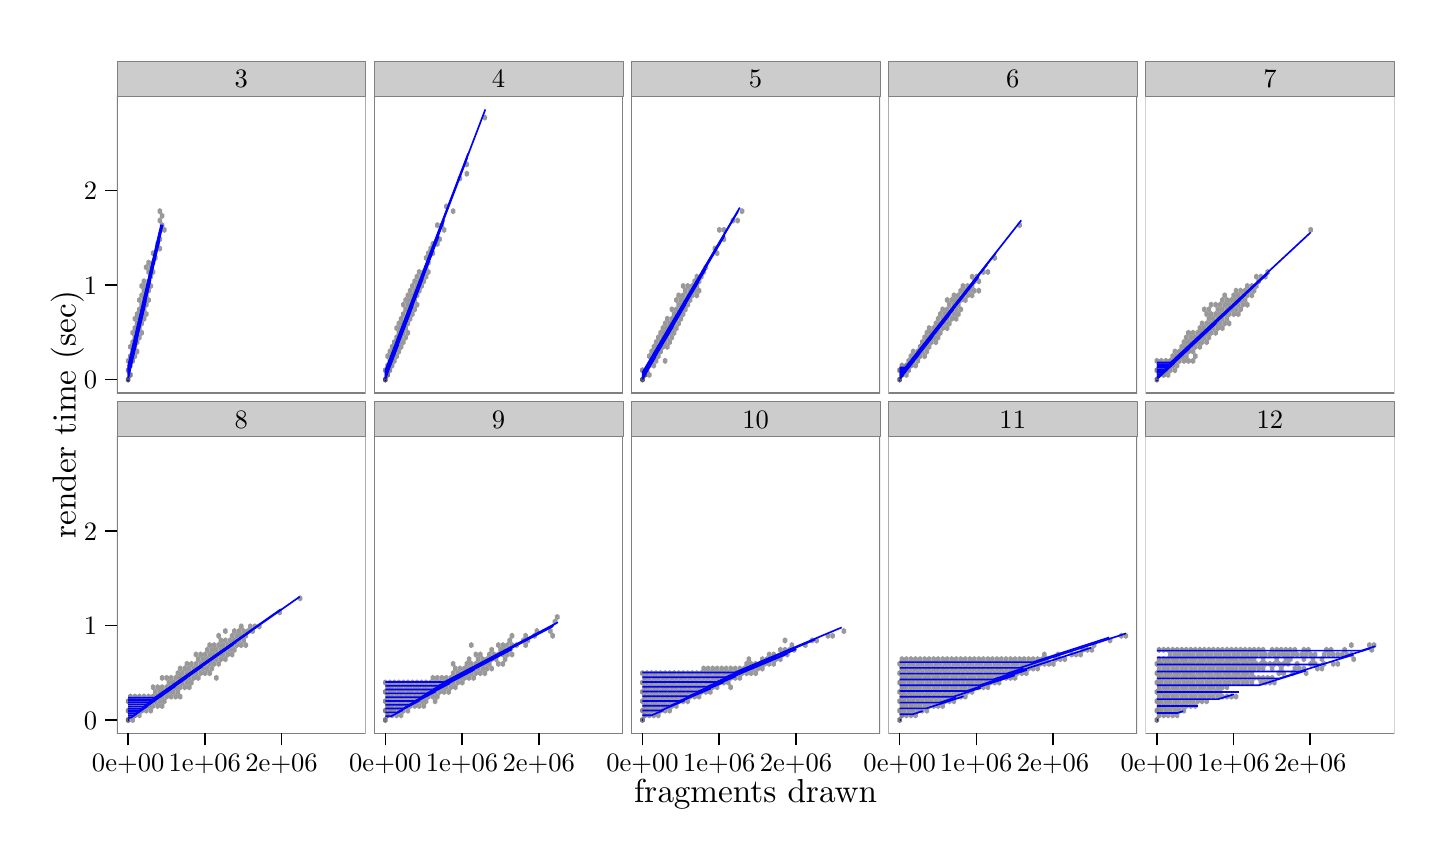
\begin{tikzpicture}[x=1pt,y=1pt]
\definecolor[named]{fillColor}{rgb}{1.00,1.00,1.00}
\path[use as bounding box,fill=fillColor,fill opacity=0.00] (0,0) rectangle (505.89,289.08);
\begin{scope}
\path[clip] (  0.00,  0.00) rectangle (505.89,289.08);
\definecolor[named]{drawColor}{rgb}{1.00,1.00,1.00}
\definecolor[named]{fillColor}{rgb}{1.00,1.00,1.00}

\path[draw=drawColor,line width= 0.6pt,line join=round,line cap=round,fill=fillColor] (  0.00,  0.00) rectangle (505.89,289.08);
\end{scope}
\begin{scope}
\path[clip] ( 32.22,157.04) rectangle (122.14,264.40);
\definecolor[named]{fillColor}{rgb}{1.00,1.00,1.00}

\path[fill=fillColor] ( 32.22,157.04) rectangle (122.14,264.40);
\definecolor[named]{fillColor}{rgb}{0.35,0.35,0.35}

\path[fill=fillColor] ( 37.13,162.48) --
	( 37.13,161.36) --
	( 36.31,160.80) --
	( 35.49,161.36) --
	( 35.49,162.48) --
	( 36.31,163.04) --
	cycle;
\definecolor[named]{fillColor}{rgb}{0.49,0.49,0.49}

\path[fill=fillColor] ( 37.94,164.17) --
	( 37.94,163.05) --
	( 37.13,162.49) --
	( 36.31,163.05) --
	( 36.31,164.17) --
	( 37.13,164.73) --
	cycle;
\definecolor[named]{fillColor}{rgb}{0.53,0.53,0.53}

\path[fill=fillColor] ( 37.13,165.86) --
	( 37.13,164.74) --
	( 36.31,164.18) --
	( 35.49,164.74) --
	( 35.49,165.86) --
	( 36.31,166.42) --
	cycle;
\definecolor[named]{fillColor}{rgb}{0.52,0.52,0.52}

\path[fill=fillColor] ( 37.94,167.55) --
	( 37.94,166.43) --
	( 37.13,165.87) --
	( 36.31,166.43) --
	( 36.31,167.55) --
	( 37.13,168.11) --
	cycle;
\definecolor[named]{fillColor}{rgb}{0.60,0.60,0.60}

\path[fill=fillColor] ( 37.13,169.24) --
	( 37.13,168.12) --
	( 36.31,167.56) --
	( 35.49,168.12) --
	( 35.49,169.24) --
	( 36.31,169.80) --
	cycle;
\definecolor[named]{fillColor}{rgb}{0.55,0.55,0.55}

\path[fill=fillColor] ( 38.76,169.24) --
	( 38.76,168.12) --
	( 37.94,167.56) --
	( 37.13,168.12) --
	( 37.13,169.24) --
	( 37.94,169.80) --
	cycle;
\definecolor[named]{fillColor}{rgb}{0.56,0.56,0.56}

\path[fill=fillColor] ( 37.94,170.93) --
	( 37.94,169.81) --
	( 37.13,169.25) --
	( 36.31,169.81) --
	( 36.31,170.93) --
	( 37.13,171.50) --
	cycle;
\definecolor[named]{fillColor}{rgb}{0.58,0.58,0.58}

\path[fill=fillColor] ( 39.58,170.93) --
	( 39.58,169.81) --
	( 38.76,169.25) --
	( 37.94,169.81) --
	( 37.94,170.93) --
	( 38.76,171.50) --
	cycle;
\definecolor[named]{fillColor}{rgb}{0.55,0.55,0.55}

\path[fill=fillColor] ( 38.76,172.62) --
	( 38.76,171.50) --
	( 37.94,170.94) --
	( 37.13,171.50) --
	( 37.13,172.62) --
	( 37.94,173.19) --
	cycle;
\definecolor[named]{fillColor}{rgb}{0.60,0.60,0.60}

\path[fill=fillColor] ( 40.40,172.62) --
	( 40.40,171.50) --
	( 39.58,170.94) --
	( 38.76,171.50) --
	( 38.76,172.62) --
	( 39.58,173.19) --
	cycle;
\definecolor[named]{fillColor}{rgb}{0.59,0.59,0.59}

\path[fill=fillColor] ( 37.94,174.32) --
	( 37.94,173.19) --
	( 37.13,172.63) --
	( 36.31,173.19) --
	( 36.31,174.32) --
	( 37.13,174.88) --
	cycle;
\definecolor[named]{fillColor}{rgb}{0.56,0.56,0.56}

\path[fill=fillColor] ( 39.58,174.32) --
	( 39.58,173.19) --
	( 38.76,172.63) --
	( 37.94,173.19) --
	( 37.94,174.32) --
	( 38.76,174.88) --
	cycle;
\definecolor[named]{fillColor}{rgb}{0.58,0.58,0.58}

\path[fill=fillColor] ( 38.76,176.01) --
	( 38.76,174.88) --
	( 37.94,174.32) --
	( 37.13,174.88) --
	( 37.13,176.01) --
	( 37.94,176.57) --
	cycle;
\definecolor[named]{fillColor}{rgb}{0.58,0.58,0.58}

\path[fill=fillColor] ( 40.40,176.01) --
	( 40.40,174.88) --
	( 39.58,174.32) --
	( 38.76,174.88) --
	( 38.76,176.01) --
	( 39.58,176.57) --
	cycle;
\definecolor[named]{fillColor}{rgb}{0.56,0.56,0.56}

\path[fill=fillColor] ( 39.58,177.70) --
	( 39.58,176.57) --
	( 38.76,176.01) --
	( 37.94,176.57) --
	( 37.94,177.70) --
	( 38.76,178.26) --
	cycle;
\definecolor[named]{fillColor}{rgb}{0.60,0.60,0.60}

\path[fill=fillColor] ( 41.21,177.70) --
	( 41.21,176.57) --
	( 40.40,176.01) --
	( 39.58,176.57) --
	( 39.58,177.70) --
	( 40.40,178.26) --
	cycle;

\path[fill=fillColor] ( 38.76,179.39) --
	( 38.76,178.26) --
	( 37.94,177.70) --
	( 37.13,178.26) --
	( 37.13,179.39) --
	( 37.94,179.95) --
	cycle;
\definecolor[named]{fillColor}{rgb}{0.57,0.57,0.57}

\path[fill=fillColor] ( 40.40,179.39) --
	( 40.40,178.26) --
	( 39.58,177.70) --
	( 38.76,178.26) --
	( 38.76,179.39) --
	( 39.58,179.95) --
	cycle;
\definecolor[named]{fillColor}{rgb}{0.60,0.60,0.60}

\path[fill=fillColor] ( 42.03,179.39) --
	( 42.03,178.26) --
	( 41.21,177.70) --
	( 40.40,178.26) --
	( 40.40,179.39) --
	( 41.21,179.95) --
	cycle;
\definecolor[named]{fillColor}{rgb}{0.59,0.59,0.59}

\path[fill=fillColor] ( 39.58,181.08) --
	( 39.58,179.95) --
	( 38.76,179.39) --
	( 37.94,179.95) --
	( 37.94,181.08) --
	( 38.76,181.64) --
	cycle;
\definecolor[named]{fillColor}{rgb}{0.58,0.58,0.58}

\path[fill=fillColor] ( 41.21,181.08) --
	( 41.21,179.95) --
	( 40.40,179.39) --
	( 39.58,179.95) --
	( 39.58,181.08) --
	( 40.40,181.64) --
	cycle;
\definecolor[named]{fillColor}{rgb}{0.58,0.58,0.58}

\path[fill=fillColor] ( 40.40,182.77) --
	( 40.40,181.65) --
	( 39.58,181.08) --
	( 38.76,181.65) --
	( 38.76,182.77) --
	( 39.58,183.33) --
	cycle;
\definecolor[named]{fillColor}{rgb}{0.59,0.59,0.59}

\path[fill=fillColor] ( 42.03,182.77) --
	( 42.03,181.65) --
	( 41.21,181.08) --
	( 40.40,181.65) --
	( 40.40,182.77) --
	( 41.21,183.33) --
	cycle;
\definecolor[named]{fillColor}{rgb}{0.60,0.60,0.60}

\path[fill=fillColor] ( 39.58,184.46) --
	( 39.58,183.34) --
	( 38.76,182.77) --
	( 37.94,183.34) --
	( 37.94,184.46) --
	( 38.76,185.02) --
	cycle;
\definecolor[named]{fillColor}{rgb}{0.58,0.58,0.58}

\path[fill=fillColor] ( 41.21,184.46) --
	( 41.21,183.34) --
	( 40.40,182.77) --
	( 39.58,183.34) --
	( 39.58,184.46) --
	( 40.40,185.02) --
	cycle;
\definecolor[named]{fillColor}{rgb}{0.59,0.59,0.59}

\path[fill=fillColor] ( 42.85,184.46) --
	( 42.85,183.34) --
	( 42.03,182.77) --
	( 41.21,183.34) --
	( 41.21,184.46) --
	( 42.03,185.02) --
	cycle;
\definecolor[named]{fillColor}{rgb}{0.59,0.59,0.59}

\path[fill=fillColor] ( 40.40,186.15) --
	( 40.40,185.03) --
	( 39.58,184.46) --
	( 38.76,185.03) --
	( 38.76,186.15) --
	( 39.58,186.71) --
	cycle;
\definecolor[named]{fillColor}{rgb}{0.58,0.58,0.58}

\path[fill=fillColor] ( 42.03,186.15) --
	( 42.03,185.03) --
	( 41.21,184.46) --
	( 40.40,185.03) --
	( 40.40,186.15) --
	( 41.21,186.71) --
	cycle;
\definecolor[named]{fillColor}{rgb}{0.60,0.60,0.60}

\path[fill=fillColor] ( 43.67,186.15) --
	( 43.67,185.03) --
	( 42.85,184.46) --
	( 42.03,185.03) --
	( 42.03,186.15) --
	( 42.85,186.71) --
	cycle;
\definecolor[named]{fillColor}{rgb}{0.58,0.58,0.58}

\path[fill=fillColor] ( 41.21,187.84) --
	( 41.21,186.72) --
	( 40.40,186.16) --
	( 39.58,186.72) --
	( 39.58,187.84) --
	( 40.40,188.40) --
	cycle;
\definecolor[named]{fillColor}{rgb}{0.59,0.59,0.59}

\path[fill=fillColor] ( 42.85,187.84) --
	( 42.85,186.72) --
	( 42.03,186.16) --
	( 41.21,186.72) --
	( 41.21,187.84) --
	( 42.03,188.40) --
	cycle;

\path[fill=fillColor] ( 42.03,189.53) --
	( 42.03,188.41) --
	( 41.21,187.85) --
	( 40.40,188.41) --
	( 40.40,189.53) --
	( 41.21,190.09) --
	cycle;
\definecolor[named]{fillColor}{rgb}{0.59,0.59,0.59}

\path[fill=fillColor] ( 43.67,189.53) --
	( 43.67,188.41) --
	( 42.85,187.85) --
	( 42.03,188.41) --
	( 42.03,189.53) --
	( 42.85,190.09) --
	cycle;
\definecolor[named]{fillColor}{rgb}{0.60,0.60,0.60}

\path[fill=fillColor] ( 41.21,191.22) --
	( 41.21,190.10) --
	( 40.40,189.54) --
	( 39.58,190.10) --
	( 39.58,191.22) --
	( 40.40,191.78) --
	cycle;
\definecolor[named]{fillColor}{rgb}{0.58,0.58,0.58}

\path[fill=fillColor] ( 42.85,191.22) --
	( 42.85,190.10) --
	( 42.03,189.54) --
	( 41.21,190.10) --
	( 41.21,191.22) --
	( 42.03,191.78) --
	cycle;
\definecolor[named]{fillColor}{rgb}{0.60,0.60,0.60}

\path[fill=fillColor] ( 44.48,191.22) --
	( 44.48,190.10) --
	( 43.67,189.54) --
	( 42.85,190.10) --
	( 42.85,191.22) --
	( 43.67,191.78) --
	cycle;

\path[fill=fillColor] ( 42.03,192.91) --
	( 42.03,191.79) --
	( 41.21,191.23) --
	( 40.40,191.79) --
	( 40.40,192.91) --
	( 41.21,193.47) --
	cycle;

\path[fill=fillColor] ( 43.67,192.91) --
	( 43.67,191.79) --
	( 42.85,191.23) --
	( 42.03,191.79) --
	( 42.03,192.91) --
	( 42.85,193.47) --
	cycle;
\definecolor[named]{fillColor}{rgb}{0.59,0.59,0.59}

\path[fill=fillColor] ( 42.85,194.60) --
	( 42.85,193.48) --
	( 42.03,192.92) --
	( 41.21,193.48) --
	( 41.21,194.60) --
	( 42.03,195.16) --
	cycle;
\definecolor[named]{fillColor}{rgb}{0.60,0.60,0.60}

\path[fill=fillColor] ( 44.48,194.60) --
	( 44.48,193.48) --
	( 43.67,192.92) --
	( 42.85,193.48) --
	( 42.85,194.60) --
	( 43.67,195.16) --
	cycle;
\definecolor[named]{fillColor}{rgb}{0.60,0.60,0.60}

\path[fill=fillColor] ( 42.03,196.29) --
	( 42.03,195.17) --
	( 41.21,194.61) --
	( 40.40,195.17) --
	( 40.40,196.29) --
	( 41.21,196.85) --
	cycle;
\definecolor[named]{fillColor}{rgb}{0.60,0.60,0.60}

\path[fill=fillColor] ( 43.67,196.29) --
	( 43.67,195.17) --
	( 42.85,194.61) --
	( 42.03,195.17) --
	( 42.03,196.29) --
	( 42.85,196.85) --
	cycle;
\definecolor[named]{fillColor}{rgb}{0.60,0.60,0.60}

\path[fill=fillColor] ( 45.30,196.29) --
	( 45.30,195.17) --
	( 44.48,194.61) --
	( 43.67,195.17) --
	( 43.67,196.29) --
	( 44.48,196.85) --
	cycle;

\path[fill=fillColor] ( 42.85,197.98) --
	( 42.85,196.86) --
	( 42.03,196.30) --
	( 41.21,196.86) --
	( 41.21,197.98) --
	( 42.03,198.54) --
	cycle;

\path[fill=fillColor] ( 44.48,197.98) --
	( 44.48,196.86) --
	( 43.67,196.30) --
	( 42.85,196.86) --
	( 42.85,197.98) --
	( 43.67,198.54) --
	cycle;

\path[fill=fillColor] ( 45.30,199.67) --
	( 45.30,198.55) --
	( 44.48,197.99) --
	( 43.67,198.55) --
	( 43.67,199.67) --
	( 44.48,200.23) --
	cycle;

\path[fill=fillColor] ( 44.48,201.36) --
	( 44.48,200.24) --
	( 43.67,199.68) --
	( 42.85,200.24) --
	( 42.85,201.36) --
	( 43.67,201.92) --
	cycle;

\path[fill=fillColor] ( 46.12,201.36) --
	( 46.12,200.24) --
	( 45.30,199.68) --
	( 44.48,200.24) --
	( 44.48,201.36) --
	( 45.30,201.92) --
	cycle;

\path[fill=fillColor] ( 43.67,203.05) --
	( 43.67,201.93) --
	( 42.85,201.37) --
	( 42.03,201.93) --
	( 42.03,203.05) --
	( 42.85,203.61) --
	cycle;

\path[fill=fillColor] ( 45.30,203.05) --
	( 45.30,201.93) --
	( 44.48,201.37) --
	( 43.67,201.93) --
	( 43.67,203.05) --
	( 44.48,203.61) --
	cycle;

\path[fill=fillColor] ( 44.48,204.74) --
	( 44.48,203.62) --
	( 43.67,203.06) --
	( 42.85,203.62) --
	( 42.85,204.74) --
	( 43.67,205.30) --
	cycle;

\path[fill=fillColor] ( 46.12,204.74) --
	( 46.12,203.62) --
	( 45.30,203.06) --
	( 44.48,203.62) --
	( 44.48,204.74) --
	( 45.30,205.30) --
	cycle;

\path[fill=fillColor] ( 46.94,206.43) --
	( 46.94,205.31) --
	( 46.12,204.75) --
	( 45.30,205.31) --
	( 45.30,206.43) --
	( 46.12,207.00) --
	cycle;

\path[fill=fillColor] ( 46.12,208.12) --
	( 46.12,207.00) --
	( 45.30,206.44) --
	( 44.48,207.00) --
	( 44.48,208.12) --
	( 45.30,208.69) --
	cycle;

\path[fill=fillColor] ( 48.57,209.82) --
	( 48.57,208.69) --
	( 47.75,208.13) --
	( 46.94,208.69) --
	( 46.94,209.82) --
	( 47.75,210.38) --
	cycle;

\path[fill=fillColor] ( 47.75,211.51) --
	( 47.75,210.38) --
	( 46.94,209.82) --
	( 46.12,210.38) --
	( 46.12,211.51) --
	( 46.94,212.07) --
	cycle;

\path[fill=fillColor] ( 48.57,213.20) --
	( 48.57,212.07) --
	( 47.75,211.51) --
	( 46.94,212.07) --
	( 46.94,213.20) --
	( 47.75,213.76) --
	cycle;

\path[fill=fillColor] ( 50.20,216.58) --
	( 50.20,215.45) --
	( 49.39,214.89) --
	( 48.57,215.45) --
	( 48.57,216.58) --
	( 49.39,217.14) --
	cycle;

\path[fill=fillColor] ( 49.39,218.27) --
	( 49.39,217.15) --
	( 48.57,216.58) --
	( 47.75,217.15) --
	( 47.75,218.27) --
	( 48.57,218.83) --
	cycle;

\path[fill=fillColor] ( 48.57,219.96) --
	( 48.57,218.84) --
	( 47.75,218.27) --
	( 46.94,218.84) --
	( 46.94,219.96) --
	( 47.75,220.52) --
	cycle;

\path[fill=fillColor] ( 49.39,221.65) --
	( 49.39,220.53) --
	( 48.57,219.96) --
	( 47.75,220.53) --
	( 47.75,221.65) --
	( 48.57,222.21) --
	cycle;

\path[fill=fillColor] ( 48.57,223.34) --
	( 48.57,222.22) --
	( 47.75,221.66) --
	( 46.94,222.22) --
	( 46.94,223.34) --
	( 47.75,223.90) --
	cycle;
\definecolor[named]{drawColor}{rgb}{0.00,0.00,1.00}

\path[draw=drawColor,line width= 0.6pt,line join=round] ( 36.31,161.92) --
	( 36.31,161.92) --
	( 36.31,161.92) --
	( 36.31,161.92) --
	( 36.31,161.92) --
	( 36.31,161.92) --
	( 36.31,161.92) --
	( 36.31,161.92) --
	( 36.31,161.92) --
	( 36.31,161.92) --
	( 36.31,161.92) --
	( 36.31,161.92) --
	( 36.31,161.92) --
	( 36.31,161.93) --
	( 36.31,161.93) --
	( 36.31,161.93) --
	( 36.31,161.93) --
	( 36.31,161.93) --
	( 36.31,161.93) --
	( 36.31,161.93) --
	( 36.31,161.93);

\path[draw=drawColor,line width= 0.6pt,line join=round] ( 36.31,162.41) --
	( 36.31,162.42) --
	( 36.31,162.43) --
	( 36.32,162.48) --
	( 36.35,162.57) --
	( 36.38,162.72) --
	( 36.43,162.93) --
	( 36.50,163.21) --
	( 36.58,163.58) --
	( 36.69,164.04) --
	( 36.82,164.59) --
	( 36.97,165.24) --
	( 37.14,165.99) --
	( 37.35,166.85) --
	( 37.57,167.82) --
	( 37.82,168.90) --
	( 38.10,170.09) --
	( 38.40,171.38) --
	( 38.73,172.78) --
	( 39.08,174.29) --
	( 39.46,175.89);

\path[draw=drawColor,line width= 0.6pt,line join=round] ( 36.31,162.91) --
	( 36.31,162.91) --
	( 36.32,162.95) --
	( 36.34,163.05) --
	( 36.39,163.23) --
	( 36.46,163.53) --
	( 36.56,163.96) --
	( 36.69,164.55) --
	( 36.87,165.30) --
	( 37.09,166.23) --
	( 37.35,167.36) --
	( 37.66,168.69) --
	( 38.02,170.23) --
	( 38.43,171.99) --
	( 38.89,173.97) --
	( 39.41,176.17) --
	( 39.97,178.59) --
	( 40.59,181.24) --
	( 41.26,184.09) --
	( 41.98,187.17) --
	( 42.74,190.44);

\path[draw=drawColor,line width= 0.6pt,line join=round] ( 36.31,163.40) --
	( 36.31,163.41) --
	( 36.32,163.45) --
	( 36.35,163.57) --
	( 36.40,163.80) --
	( 36.49,164.16) --
	( 36.61,164.69) --
	( 36.78,165.41) --
	( 36.99,166.33) --
	( 37.26,167.49) --
	( 37.59,168.88) --
	( 37.98,170.53) --
	( 38.42,172.45) --
	( 38.94,174.65) --
	( 39.52,177.13) --
	( 40.16,179.89) --
	( 40.87,182.94) --
	( 41.66,186.28) --
	( 42.50,189.91) --
	( 43.42,193.82) --
	( 44.40,198.01);

\path[draw=drawColor,line width= 0.6pt,line join=round] ( 36.31,163.89) --
	( 36.31,163.90) --
	( 36.33,163.97) --
	( 36.37,164.14) --
	( 36.44,164.46) --
	( 36.56,164.97) --
	( 36.73,165.71) --
	( 36.97,166.72) --
	( 37.27,168.02) --
	( 37.65,169.64) --
	( 38.11,171.60) --
	( 38.65,173.92) --
	( 39.28,176.62) --
	( 40.00,179.69) --
	( 40.81,183.16) --
	( 41.72,187.03) --
	( 42.71,191.30) --
	( 43.80,195.97) --
	( 44.99,201.03) --
	( 46.26,206.48) --
	( 47.62,212.32);

\path[draw=drawColor,line width= 0.6pt,line join=round] ( 36.31,164.39) --
	( 36.31,164.40) --
	( 36.33,164.46) --
	( 36.37,164.65) --
	( 36.45,164.99) --
	( 36.58,165.55) --
	( 36.77,166.36) --
	( 37.03,167.46) --
	( 37.36,168.87) --
	( 37.77,170.64) --
	( 38.27,172.78) --
	( 38.86,175.32) --
	( 39.55,178.28) --
	( 40.34,181.66) --
	( 41.24,185.48) --
	( 42.24,189.75) --
	( 43.34,194.47) --
	( 44.55,199.64) --
	( 45.86,205.27) --
	( 47.28,211.34) --
	( 48.80,217.85);

\path[draw=drawColor,line width= 0.6pt,line join=round] ( 36.31,164.88) --
	( 36.31,164.89) --
	( 36.32,164.94) --
	( 36.36,165.10) --
	( 36.43,165.39) --
	( 36.54,165.86) --
	( 36.70,166.54) --
	( 36.91,167.47) --
	( 37.19,168.67) --
	( 37.55,170.18) --
	( 37.98,172.01) --
	( 38.49,174.19) --
	( 39.08,176.74) --
	( 39.77,179.68) --
	( 40.54,183.00) --
	( 41.42,186.74) --
	( 42.38,190.88) --
	( 43.45,195.45) --
	( 44.62,200.44) --
	( 45.88,205.85) --
	( 47.25,211.69);

\path[draw=drawColor,line width= 0.6pt,line join=round] ( 36.31,165.37) --
	( 36.31,165.38) --
	( 36.33,165.44) --
	( 36.37,165.61) --
	( 36.44,165.94) --
	( 36.56,166.46) --
	( 36.74,167.22) --
	( 36.98,168.25) --
	( 37.29,169.59) --
	( 37.69,171.27) --
	( 38.16,173.31) --
	( 38.73,175.75) --
	( 39.40,178.59) --
	( 40.16,181.87) --
	( 41.03,185.58) --
	( 42.01,189.75) --
	( 43.09,194.39) --
	( 44.28,199.50) --
	( 45.59,205.09) --
	( 47.01,211.15) --
	( 48.53,217.70);

\path[draw=drawColor,line width= 0.6pt,line join=round] ( 36.31,165.86) --
	( 36.31,165.87) --
	( 36.32,165.93) --
	( 36.36,166.09) --
	( 36.43,166.40) --
	( 36.55,166.89) --
	( 36.72,167.61) --
	( 36.94,168.59) --
	( 37.24,169.86) --
	( 37.61,171.45) --
	( 38.07,173.40) --
	( 38.61,175.72) --
	( 39.25,178.44) --
	( 39.98,181.58) --
	( 40.81,185.15) --
	( 41.75,189.16) --
	( 42.80,193.63) --
	( 43.95,198.56) --
	( 45.21,203.97) --
	( 46.59,209.86) --
	( 48.07,216.22);

\path[draw=drawColor,line width= 0.6pt,line join=round] ( 36.31,166.36) --
	( 36.31,166.37) --
	( 36.32,166.42) --
	( 36.36,166.58) --
	( 36.43,166.87) --
	( 36.54,167.35) --
	( 36.70,168.05) --
	( 36.93,169.00) --
	( 37.22,170.24) --
	( 37.58,171.79) --
	( 38.02,173.69) --
	( 38.55,175.96) --
	( 39.17,178.62) --
	( 39.89,181.69) --
	( 40.71,185.19) --
	( 41.63,189.13) --
	( 42.66,193.53) --
	( 43.79,198.39) --
	( 45.04,203.73) --
	( 46.40,209.55) --
	( 47.87,215.85);

\path[draw=drawColor,line width= 0.6pt,line join=round] ( 36.31,166.85) --
	( 36.31,166.86) --
	( 36.32,166.92) --
	( 36.36,167.08) --
	( 36.43,167.38) --
	( 36.55,167.87) --
	( 36.71,168.58) --
	( 36.94,169.56) --
	( 37.24,170.83) --
	( 37.61,172.42) --
	( 38.07,174.38) --
	( 38.61,176.71) --
	( 39.25,179.45) --
	( 39.99,182.61) --
	( 40.83,186.22) --
	( 41.78,190.28) --
	( 42.84,194.82) --
	( 44.02,199.85) --
	( 45.31,205.36) --
	( 46.71,211.38) --
	( 48.24,217.91);
\definecolor[named]{drawColor}{rgb}{0.50,0.50,0.50}

\path[draw=drawColor,line width= 0.6pt,line join=round,line cap=round] ( 32.22,157.04) rectangle (122.14,264.40);
\end{scope}
\begin{scope}
\path[clip] (125.15,157.04) rectangle (215.06,264.40);
\definecolor[named]{fillColor}{rgb}{1.00,1.00,1.00}

\path[fill=fillColor] (125.15,157.04) rectangle (215.06,264.40);
\definecolor[named]{fillColor}{rgb}{0.30,0.30,0.30}

\path[fill=fillColor] (130.05,162.48) --
	(130.05,161.36) --
	(129.24,160.80) --
	(128.42,161.36) --
	(128.42,162.48) --
	(129.24,163.04) --
	cycle;
\definecolor[named]{fillColor}{rgb}{0.45,0.45,0.45}

\path[fill=fillColor] (130.87,164.17) --
	(130.87,163.05) --
	(130.05,162.49) --
	(129.24,163.05) --
	(129.24,164.17) --
	(130.05,164.73) --
	cycle;
\definecolor[named]{fillColor}{rgb}{0.56,0.56,0.56}

\path[fill=fillColor] (130.05,165.86) --
	(130.05,164.74) --
	(129.24,164.18) --
	(128.42,164.74) --
	(128.42,165.86) --
	(129.24,166.42) --
	cycle;
\definecolor[named]{fillColor}{rgb}{0.55,0.55,0.55}

\path[fill=fillColor] (131.69,165.86) --
	(131.69,164.74) --
	(130.87,164.18) --
	(130.05,164.74) --
	(130.05,165.86) --
	(130.87,166.42) --
	cycle;
\definecolor[named]{fillColor}{rgb}{0.53,0.53,0.53}

\path[fill=fillColor] (130.87,167.55) --
	(130.87,166.43) --
	(130.05,165.87) --
	(129.24,166.43) --
	(129.24,167.55) --
	(130.05,168.11) --
	cycle;
\definecolor[named]{fillColor}{rgb}{0.58,0.58,0.58}

\path[fill=fillColor] (132.51,167.55) --
	(132.51,166.43) --
	(131.69,165.87) --
	(130.87,166.43) --
	(130.87,167.55) --
	(131.69,168.11) --
	cycle;
\definecolor[named]{fillColor}{rgb}{0.53,0.53,0.53}

\path[fill=fillColor] (131.69,169.24) --
	(131.69,168.12) --
	(130.87,167.56) --
	(130.05,168.12) --
	(130.05,169.24) --
	(130.87,169.80) --
	cycle;
\definecolor[named]{fillColor}{rgb}{0.59,0.59,0.59}

\path[fill=fillColor] (133.32,169.24) --
	(133.32,168.12) --
	(132.51,167.56) --
	(131.69,168.12) --
	(131.69,169.24) --
	(132.51,169.80) --
	cycle;
\definecolor[named]{fillColor}{rgb}{0.60,0.60,0.60}

\path[fill=fillColor] (130.87,170.93) --
	(130.87,169.81) --
	(130.05,169.25) --
	(129.24,169.81) --
	(129.24,170.93) --
	(130.05,171.50) --
	cycle;
\definecolor[named]{fillColor}{rgb}{0.54,0.54,0.54}

\path[fill=fillColor] (132.51,170.93) --
	(132.51,169.81) --
	(131.69,169.25) --
	(130.87,169.81) --
	(130.87,170.93) --
	(131.69,171.50) --
	cycle;
\definecolor[named]{fillColor}{rgb}{0.60,0.60,0.60}

\path[fill=fillColor] (134.14,170.93) --
	(134.14,169.81) --
	(133.32,169.25) --
	(132.51,169.81) --
	(132.51,170.93) --
	(133.32,171.50) --
	cycle;

\path[fill=fillColor] (131.69,172.62) --
	(131.69,171.50) --
	(130.87,170.94) --
	(130.05,171.50) --
	(130.05,172.62) --
	(130.87,173.19) --
	cycle;
\definecolor[named]{fillColor}{rgb}{0.56,0.56,0.56}

\path[fill=fillColor] (133.32,172.62) --
	(133.32,171.50) --
	(132.51,170.94) --
	(131.69,171.50) --
	(131.69,172.62) --
	(132.51,173.19) --
	cycle;
\definecolor[named]{fillColor}{rgb}{0.60,0.60,0.60}

\path[fill=fillColor] (134.96,172.62) --
	(134.96,171.50) --
	(134.14,170.94) --
	(133.32,171.50) --
	(133.32,172.62) --
	(134.14,173.19) --
	cycle;
\definecolor[named]{fillColor}{rgb}{0.58,0.58,0.58}

\path[fill=fillColor] (132.51,174.32) --
	(132.51,173.19) --
	(131.69,172.63) --
	(130.87,173.19) --
	(130.87,174.32) --
	(131.69,174.88) --
	cycle;
\definecolor[named]{fillColor}{rgb}{0.57,0.57,0.57}

\path[fill=fillColor] (134.14,174.32) --
	(134.14,173.19) --
	(133.32,172.63) --
	(132.51,173.19) --
	(132.51,174.32) --
	(133.32,174.88) --
	cycle;
\definecolor[named]{fillColor}{rgb}{0.60,0.60,0.60}

\path[fill=fillColor] (135.77,174.32) --
	(135.77,173.19) --
	(134.96,172.63) --
	(134.14,173.19) --
	(134.14,174.32) --
	(134.96,174.88) --
	cycle;
\definecolor[named]{fillColor}{rgb}{0.58,0.58,0.58}

\path[fill=fillColor] (133.32,176.01) --
	(133.32,174.88) --
	(132.51,174.32) --
	(131.69,174.88) --
	(131.69,176.01) --
	(132.51,176.57) --
	cycle;

\path[fill=fillColor] (134.96,176.01) --
	(134.96,174.88) --
	(134.14,174.32) --
	(133.32,174.88) --
	(133.32,176.01) --
	(134.14,176.57) --
	cycle;
\definecolor[named]{fillColor}{rgb}{0.60,0.60,0.60}

\path[fill=fillColor] (136.59,176.01) --
	(136.59,174.88) --
	(135.77,174.32) --
	(134.96,174.88) --
	(134.96,176.01) --
	(135.77,176.57) --
	cycle;
\definecolor[named]{fillColor}{rgb}{0.57,0.57,0.57}

\path[fill=fillColor] (134.14,177.70) --
	(134.14,176.57) --
	(133.32,176.01) --
	(132.51,176.57) --
	(132.51,177.70) --
	(133.32,178.26) --
	cycle;
\definecolor[named]{fillColor}{rgb}{0.58,0.58,0.58}

\path[fill=fillColor] (135.77,177.70) --
	(135.77,176.57) --
	(134.96,176.01) --
	(134.14,176.57) --
	(134.14,177.70) --
	(134.96,178.26) --
	cycle;
\definecolor[named]{fillColor}{rgb}{0.60,0.60,0.60}

\path[fill=fillColor] (137.41,177.70) --
	(137.41,176.57) --
	(136.59,176.01) --
	(135.77,176.57) --
	(135.77,177.70) --
	(136.59,178.26) --
	cycle;
\definecolor[named]{fillColor}{rgb}{0.58,0.58,0.58}

\path[fill=fillColor] (134.96,179.39) --
	(134.96,178.26) --
	(134.14,177.70) --
	(133.32,178.26) --
	(133.32,179.39) --
	(134.14,179.95) --
	cycle;
\definecolor[named]{fillColor}{rgb}{0.59,0.59,0.59}

\path[fill=fillColor] (136.59,179.39) --
	(136.59,178.26) --
	(135.77,177.70) --
	(134.96,178.26) --
	(134.96,179.39) --
	(135.77,179.95) --
	cycle;
\definecolor[named]{fillColor}{rgb}{0.60,0.60,0.60}

\path[fill=fillColor] (138.23,179.39) --
	(138.23,178.26) --
	(137.41,177.70) --
	(136.59,178.26) --
	(136.59,179.39) --
	(137.41,179.95) --
	cycle;
\definecolor[named]{fillColor}{rgb}{0.60,0.60,0.60}

\path[fill=fillColor] (134.14,181.08) --
	(134.14,179.95) --
	(133.32,179.39) --
	(132.51,179.95) --
	(132.51,181.08) --
	(133.32,181.64) --
	cycle;
\definecolor[named]{fillColor}{rgb}{0.58,0.58,0.58}

\path[fill=fillColor] (135.77,181.08) --
	(135.77,179.95) --
	(134.96,179.39) --
	(134.14,179.95) --
	(134.14,181.08) --
	(134.96,181.64) --
	cycle;
\definecolor[named]{fillColor}{rgb}{0.59,0.59,0.59}

\path[fill=fillColor] (137.41,181.08) --
	(137.41,179.95) --
	(136.59,179.39) --
	(135.77,179.95) --
	(135.77,181.08) --
	(136.59,181.64) --
	cycle;
\definecolor[named]{fillColor}{rgb}{0.60,0.60,0.60}

\path[fill=fillColor] (134.96,182.77) --
	(134.96,181.65) --
	(134.14,181.08) --
	(133.32,181.65) --
	(133.32,182.77) --
	(134.14,183.33) --
	cycle;
\definecolor[named]{fillColor}{rgb}{0.58,0.58,0.58}

\path[fill=fillColor] (136.59,182.77) --
	(136.59,181.65) --
	(135.77,181.08) --
	(134.96,181.65) --
	(134.96,182.77) --
	(135.77,183.33) --
	cycle;
\definecolor[named]{fillColor}{rgb}{0.60,0.60,0.60}

\path[fill=fillColor] (138.23,182.77) --
	(138.23,181.65) --
	(137.41,181.08) --
	(136.59,181.65) --
	(136.59,182.77) --
	(137.41,183.33) --
	cycle;
\definecolor[named]{fillColor}{rgb}{0.59,0.59,0.59}

\path[fill=fillColor] (135.77,184.46) --
	(135.77,183.34) --
	(134.96,182.77) --
	(134.14,183.34) --
	(134.14,184.46) --
	(134.96,185.02) --
	cycle;
\definecolor[named]{fillColor}{rgb}{0.58,0.58,0.58}

\path[fill=fillColor] (137.41,184.46) --
	(137.41,183.34) --
	(136.59,182.77) --
	(135.77,183.34) --
	(135.77,184.46) --
	(136.59,185.02) --
	cycle;
\definecolor[named]{fillColor}{rgb}{0.60,0.60,0.60}

\path[fill=fillColor] (139.04,184.46) --
	(139.04,183.34) --
	(138.23,182.77) --
	(137.41,183.34) --
	(137.41,184.46) --
	(138.23,185.02) --
	cycle;
\definecolor[named]{fillColor}{rgb}{0.59,0.59,0.59}

\path[fill=fillColor] (136.59,186.15) --
	(136.59,185.03) --
	(135.77,184.46) --
	(134.96,185.03) --
	(134.96,186.15) --
	(135.77,186.71) --
	cycle;
\definecolor[named]{fillColor}{rgb}{0.59,0.59,0.59}

\path[fill=fillColor] (138.23,186.15) --
	(138.23,185.03) --
	(137.41,184.46) --
	(136.59,185.03) --
	(136.59,186.15) --
	(137.41,186.71) --
	cycle;
\definecolor[named]{fillColor}{rgb}{0.60,0.60,0.60}

\path[fill=fillColor] (139.86,186.15) --
	(139.86,185.03) --
	(139.04,184.46) --
	(138.23,185.03) --
	(138.23,186.15) --
	(139.04,186.71) --
	cycle;
\definecolor[named]{fillColor}{rgb}{0.59,0.59,0.59}

\path[fill=fillColor] (137.41,187.84) --
	(137.41,186.72) --
	(136.59,186.16) --
	(135.77,186.72) --
	(135.77,187.84) --
	(136.59,188.40) --
	cycle;

\path[fill=fillColor] (139.04,187.84) --
	(139.04,186.72) --
	(138.23,186.16) --
	(137.41,186.72) --
	(137.41,187.84) --
	(138.23,188.40) --
	cycle;
\definecolor[named]{fillColor}{rgb}{0.60,0.60,0.60}

\path[fill=fillColor] (140.68,187.84) --
	(140.68,186.72) --
	(139.86,186.16) --
	(139.04,186.72) --
	(139.04,187.84) --
	(139.86,188.40) --
	cycle;
\definecolor[named]{fillColor}{rgb}{0.60,0.60,0.60}

\path[fill=fillColor] (136.59,189.53) --
	(136.59,188.41) --
	(135.77,187.85) --
	(134.96,188.41) --
	(134.96,189.53) --
	(135.77,190.09) --
	cycle;
\definecolor[named]{fillColor}{rgb}{0.59,0.59,0.59}

\path[fill=fillColor] (138.23,189.53) --
	(138.23,188.41) --
	(137.41,187.85) --
	(136.59,188.41) --
	(136.59,189.53) --
	(137.41,190.09) --
	cycle;

\path[fill=fillColor] (139.86,189.53) --
	(139.86,188.41) --
	(139.04,187.85) --
	(138.23,188.41) --
	(138.23,189.53) --
	(139.04,190.09) --
	cycle;
\definecolor[named]{fillColor}{rgb}{0.60,0.60,0.60}

\path[fill=fillColor] (141.50,189.53) --
	(141.50,188.41) --
	(140.68,187.85) --
	(139.86,188.41) --
	(139.86,189.53) --
	(140.68,190.09) --
	cycle;
\definecolor[named]{fillColor}{rgb}{0.60,0.60,0.60}

\path[fill=fillColor] (137.41,191.22) --
	(137.41,190.10) --
	(136.59,189.54) --
	(135.77,190.10) --
	(135.77,191.22) --
	(136.59,191.78) --
	cycle;
\definecolor[named]{fillColor}{rgb}{0.59,0.59,0.59}

\path[fill=fillColor] (139.04,191.22) --
	(139.04,190.10) --
	(138.23,189.54) --
	(137.41,190.10) --
	(137.41,191.22) --
	(138.23,191.78) --
	cycle;
\definecolor[named]{fillColor}{rgb}{0.60,0.60,0.60}

\path[fill=fillColor] (140.68,191.22) --
	(140.68,190.10) --
	(139.86,189.54) --
	(139.04,190.10) --
	(139.04,191.22) --
	(139.86,191.78) --
	cycle;

\path[fill=fillColor] (138.23,192.91) --
	(138.23,191.79) --
	(137.41,191.23) --
	(136.59,191.79) --
	(136.59,192.91) --
	(137.41,193.47) --
	cycle;

\path[fill=fillColor] (139.86,192.91) --
	(139.86,191.79) --
	(139.04,191.23) --
	(138.23,191.79) --
	(138.23,192.91) --
	(139.04,193.47) --
	cycle;

\path[fill=fillColor] (141.50,192.91) --
	(141.50,191.79) --
	(140.68,191.23) --
	(139.86,191.79) --
	(139.86,192.91) --
	(140.68,193.47) --
	cycle;

\path[fill=fillColor] (139.04,194.60) --
	(139.04,193.48) --
	(138.23,192.92) --
	(137.41,193.48) --
	(137.41,194.60) --
	(138.23,195.16) --
	cycle;

\path[fill=fillColor] (140.68,194.60) --
	(140.68,193.48) --
	(139.86,192.92) --
	(139.04,193.48) --
	(139.04,194.60) --
	(139.86,195.16) --
	cycle;

\path[fill=fillColor] (142.31,194.60) --
	(142.31,193.48) --
	(141.50,192.92) --
	(140.68,193.48) --
	(140.68,194.60) --
	(141.50,195.16) --
	cycle;
\definecolor[named]{fillColor}{rgb}{0.60,0.60,0.60}

\path[fill=fillColor] (139.86,196.29) --
	(139.86,195.17) --
	(139.04,194.61) --
	(138.23,195.17) --
	(138.23,196.29) --
	(139.04,196.85) --
	cycle;
\definecolor[named]{fillColor}{rgb}{0.60,0.60,0.60}

\path[fill=fillColor] (141.50,196.29) --
	(141.50,195.17) --
	(140.68,194.61) --
	(139.86,195.17) --
	(139.86,196.29) --
	(140.68,196.85) --
	cycle;
\definecolor[named]{fillColor}{rgb}{0.60,0.60,0.60}

\path[fill=fillColor] (143.13,196.29) --
	(143.13,195.17) --
	(142.31,194.61) --
	(141.50,195.17) --
	(141.50,196.29) --
	(142.31,196.85) --
	cycle;

\path[fill=fillColor] (140.68,197.98) --
	(140.68,196.86) --
	(139.86,196.30) --
	(139.04,196.86) --
	(139.04,197.98) --
	(139.86,198.54) --
	cycle;

\path[fill=fillColor] (142.31,197.98) --
	(142.31,196.86) --
	(141.50,196.30) --
	(140.68,196.86) --
	(140.68,197.98) --
	(141.50,198.54) --
	cycle;

\path[fill=fillColor] (143.95,197.98) --
	(143.95,196.86) --
	(143.13,196.30) --
	(142.31,196.86) --
	(142.31,197.98) --
	(143.13,198.54) --
	cycle;

\path[fill=fillColor] (141.50,199.67) --
	(141.50,198.55) --
	(140.68,197.99) --
	(139.86,198.55) --
	(139.86,199.67) --
	(140.68,200.23) --
	cycle;

\path[fill=fillColor] (143.13,199.67) --
	(143.13,198.55) --
	(142.31,197.99) --
	(141.50,198.55) --
	(141.50,199.67) --
	(142.31,200.23) --
	cycle;

\path[fill=fillColor] (144.77,199.67) --
	(144.77,198.55) --
	(143.95,197.99) --
	(143.13,198.55) --
	(143.13,199.67) --
	(143.95,200.23) --
	cycle;

\path[fill=fillColor] (142.31,201.36) --
	(142.31,200.24) --
	(141.50,199.68) --
	(140.68,200.24) --
	(140.68,201.36) --
	(141.50,201.92) --
	cycle;

\path[fill=fillColor] (143.95,201.36) --
	(143.95,200.24) --
	(143.13,199.68) --
	(142.31,200.24) --
	(142.31,201.36) --
	(143.13,201.92) --
	cycle;

\path[fill=fillColor] (145.58,201.36) --
	(145.58,200.24) --
	(144.77,199.68) --
	(143.95,200.24) --
	(143.95,201.36) --
	(144.77,201.92) --
	cycle;

\path[fill=fillColor] (144.77,203.05) --
	(144.77,201.93) --
	(143.95,201.37) --
	(143.13,201.93) --
	(143.13,203.05) --
	(143.95,203.61) --
	cycle;

\path[fill=fillColor] (145.58,204.74) --
	(145.58,203.62) --
	(144.77,203.06) --
	(143.95,203.62) --
	(143.95,204.74) --
	(144.77,205.30) --
	cycle;

\path[fill=fillColor] (144.77,206.43) --
	(144.77,205.31) --
	(143.95,204.75) --
	(143.13,205.31) --
	(143.13,206.43) --
	(143.95,207.00) --
	cycle;

\path[fill=fillColor] (145.58,208.12) --
	(145.58,207.00) --
	(144.77,206.44) --
	(143.95,207.00) --
	(143.95,208.12) --
	(144.77,208.69) --
	cycle;

\path[fill=fillColor] (147.22,208.12) --
	(147.22,207.00) --
	(146.40,206.44) --
	(145.58,207.00) --
	(145.58,208.12) --
	(146.40,208.69) --
	cycle;

\path[fill=fillColor] (146.40,209.82) --
	(146.40,208.69) --
	(145.58,208.13) --
	(144.77,208.69) --
	(144.77,209.82) --
	(145.58,210.38) --
	cycle;

\path[fill=fillColor] (147.22,211.51) --
	(147.22,210.38) --
	(146.40,209.82) --
	(145.58,210.38) --
	(145.58,211.51) --
	(146.40,212.07) --
	cycle;

\path[fill=fillColor] (148.85,211.51) --
	(148.85,210.38) --
	(148.04,209.82) --
	(147.22,210.38) --
	(147.22,211.51) --
	(148.04,212.07) --
	cycle;

\path[fill=fillColor] (149.67,213.20) --
	(149.67,212.07) --
	(148.85,211.51) --
	(148.04,212.07) --
	(148.04,213.20) --
	(148.85,213.76) --
	cycle;

\path[fill=fillColor] (151.31,216.58) --
	(151.31,215.45) --
	(150.49,214.89) --
	(149.67,215.45) --
	(149.67,216.58) --
	(150.49,217.14) --
	cycle;

\path[fill=fillColor] (148.85,218.27) --
	(148.85,217.15) --
	(148.04,216.58) --
	(147.22,217.15) --
	(147.22,218.27) --
	(148.04,218.83) --
	cycle;

\path[fill=fillColor] (150.49,218.27) --
	(150.49,217.15) --
	(149.67,216.58) --
	(148.85,217.15) --
	(148.85,218.27) --
	(149.67,218.83) --
	cycle;

\path[fill=fillColor] (154.58,223.34) --
	(154.58,222.22) --
	(153.76,221.66) --
	(152.94,222.22) --
	(152.94,223.34) --
	(153.76,223.90) --
	cycle;

\path[fill=fillColor] (152.12,225.03) --
	(152.12,223.91) --
	(151.31,223.35) --
	(150.49,223.91) --
	(150.49,225.03) --
	(151.31,225.59) --
	cycle;

\path[fill=fillColor] (157.03,235.17) --
	(157.03,234.05) --
	(156.21,233.49) --
	(155.39,234.05) --
	(155.39,235.17) --
	(156.21,235.73) --
	cycle;

\path[fill=fillColor] (159.48,236.86) --
	(159.48,235.74) --
	(158.66,235.18) --
	(157.85,235.74) --
	(157.85,236.86) --
	(158.66,237.42) --
	cycle;

\path[fill=fillColor] (159.48,240.24) --
	(159.48,239.12) --
	(158.66,238.56) --
	(157.85,239.12) --
	(157.85,240.24) --
	(158.66,240.81) --
	cycle;

\path[fill=fillColor] (166.02,257.15) --
	(166.02,256.03) --
	(165.20,255.47) --
	(164.38,256.03) --
	(164.38,257.15) --
	(165.20,257.71) --
	cycle;
\definecolor[named]{drawColor}{rgb}{0.00,0.00,1.00}

\path[draw=drawColor,line width= 0.6pt,line join=round] (129.24,161.92) --
	(129.24,161.92) --
	(129.24,161.92) --
	(129.24,161.92) --
	(129.24,161.92) --
	(129.24,161.92) --
	(129.24,161.92) --
	(129.24,161.92) --
	(129.24,161.92) --
	(129.24,161.92) --
	(129.24,161.92) --
	(129.24,161.92) --
	(129.24,161.92) --
	(129.24,161.92) --
	(129.24,161.93) --
	(129.24,161.93) --
	(129.24,161.93) --
	(129.24,161.93) --
	(129.24,161.93) --
	(129.24,161.93) --
	(129.24,161.93);

\path[draw=drawColor,line width= 0.6pt,line join=round] (129.24,162.24) --
	(129.24,162.24) --
	(129.24,162.24) --
	(129.24,162.26) --
	(129.25,162.29) --
	(129.28,162.35) --
	(129.32,162.45) --
	(129.38,162.62) --
	(129.47,162.85) --
	(129.59,163.17) --
	(129.75,163.59) --
	(129.95,164.12) --
	(130.20,164.77) --
	(130.49,165.54) --
	(130.84,166.45) --
	(131.24,167.49) --
	(131.69,168.66) --
	(132.19,169.98) --
	(132.74,171.42) --
	(133.33,172.99) --
	(133.97,174.67);

\path[draw=drawColor,line width= 0.6pt,line join=round] (129.24,162.56) --
	(129.24,162.56) --
	(129.24,162.57) --
	(129.25,162.59) --
	(129.27,162.66) --
	(129.32,162.79) --
	(129.41,163.01) --
	(129.54,163.36) --
	(129.73,163.85) --
	(129.99,164.53) --
	(130.32,165.41) --
	(130.75,166.52) --
	(131.26,167.88) --
	(131.88,169.50) --
	(132.61,171.40) --
	(133.44,173.58) --
	(134.38,176.04) --
	(135.42,178.77) --
	(136.56,181.77) --
	(137.80,185.02) --
	(139.13,188.50);

\path[draw=drawColor,line width= 0.6pt,line join=round] (129.24,162.88) --
	(129.24,162.88) --
	(129.24,162.89) --
	(129.25,162.92) --
	(129.29,163.01) --
	(129.35,163.18) --
	(129.47,163.48) --
	(129.64,163.94) --
	(129.90,164.61) --
	(130.24,165.52) --
	(130.70,166.71) --
	(131.27,168.21) --
	(131.97,170.05) --
	(132.81,172.26) --
	(133.80,174.85) --
	(134.94,177.83) --
	(136.23,181.21) --
	(137.66,184.98) --
	(139.25,189.13) --
	(140.97,193.65) --
	(142.82,198.50);

\path[draw=drawColor,line width= 0.6pt,line join=round] (129.24,163.20) --
	(129.24,163.20) --
	(129.24,163.21) --
	(129.26,163.26) --
	(129.31,163.39) --
	(129.40,163.64) --
	(129.57,164.07) --
	(129.82,164.73) --
	(130.19,165.69) --
	(130.68,167.00) --
	(131.34,168.70) --
	(132.16,170.85) --
	(133.16,173.49) --
	(134.36,176.63) --
	(135.77,180.32) --
	(137.38,184.55) --
	(139.20,189.33) --
	(141.24,194.66) --
	(143.47,200.51) --
	(145.89,206.85) --
	(148.48,213.66);

\path[draw=drawColor,line width= 0.6pt,line join=round] (129.24,163.52) --
	(129.24,163.52) --
	(129.24,163.53) --
	(129.25,163.57) --
	(129.29,163.67) --
	(129.37,163.86) --
	(129.50,164.20) --
	(129.70,164.73) --
	(129.99,165.51) --
	(130.40,166.57) --
	(130.93,167.96) --
	(131.61,169.74) --
	(132.45,171.94) --
	(133.46,174.60) --
	(134.66,177.74) --
	(136.06,181.40) --
	(137.65,185.58) --
	(139.45,190.30) --
	(141.46,195.56) --
	(143.66,201.34) --
	(146.07,207.64);

\path[draw=drawColor,line width= 0.6pt,line join=round] (129.24,163.84) --
	(129.24,163.84) --
	(129.24,163.85) --
	(129.26,163.90) --
	(129.31,164.03) --
	(129.40,164.28) --
	(129.57,164.71) --
	(129.83,165.39) --
	(130.20,166.37) --
	(130.72,167.73) --
	(131.40,169.50) --
	(132.26,171.76) --
	(133.32,174.55) --
	(134.61,177.92) --
	(136.13,181.90) --
	(137.89,186.52) --
	(139.90,191.80) --
	(142.17,197.74) --
	(144.69,204.35) --
	(147.46,211.62) --
	(150.47,219.51);

\path[draw=drawColor,line width= 0.6pt,line join=round] (129.24,164.16) --
	(129.24,164.16) --
	(129.24,164.17) --
	(129.26,164.22) --
	(129.30,164.33) --
	(129.39,164.56) --
	(129.54,164.97) --
	(129.79,165.60) --
	(130.14,166.52) --
	(130.62,167.79) --
	(131.26,169.46) --
	(132.08,171.60) --
	(133.09,174.26) --
	(134.32,177.48) --
	(135.77,181.30) --
	(137.48,185.76) --
	(139.43,190.88) --
	(141.64,196.68) --
	(144.12,203.17) --
	(146.85,210.35) --
	(149.85,218.20);

\path[draw=drawColor,line width= 0.6pt,line join=round] (129.24,164.48) --
	(129.24,164.48) --
	(129.24,164.50) --
	(129.27,164.57) --
	(129.34,164.74) --
	(129.47,165.10) --
	(129.71,165.71) --
	(130.07,166.67) --
	(130.60,168.06) --
	(131.33,169.96) --
	(132.28,172.45) --
	(133.49,175.63) --
	(134.98,179.54) --
	(136.78,184.26) --
	(138.91,189.83) --
	(141.37,196.29) --
	(144.18,203.65) --
	(147.34,211.93) --
	(150.84,221.12) --
	(154.69,231.21) --
	(158.86,242.16);

\path[draw=drawColor,line width= 0.6pt,line join=round] (129.24,164.80) --
	(129.24,164.80) --
	(129.24,164.82) --
	(129.28,164.91) --
	(129.36,165.13) --
	(129.53,165.58) --
	(129.82,166.34) --
	(130.28,167.53) --
	(130.93,169.25) --
	(131.83,171.61) --
	(133.01,174.70) --
	(134.51,178.61) --
	(136.34,183.44) --
	(138.56,189.23) --
	(141.16,196.06) --
	(144.17,203.95) --
	(147.60,212.93) --
	(151.44,223.00) --
	(155.69,234.15) --
	(160.34,246.34) --
	(165.37,259.52);

\path[draw=drawColor,line width= 0.6pt,line join=round] (129.24,165.12) --
	(129.24,165.12) --
	(129.24,165.13) --
	(129.27,165.20) --
	(129.33,165.37) --
	(129.46,165.71) --
	(129.69,166.30) --
	(130.04,167.22) --
	(130.55,168.56) --
	(131.25,170.41) --
	(132.18,172.85) --
	(133.37,175.96) --
	(134.85,179.83) --
	(136.63,184.51) --
	(138.75,190.07) --
	(141.22,196.55) --
	(144.06,203.98) --
	(147.27,212.41) --
	(150.86,221.82) --
	(154.83,232.23) --
	(159.17,243.61);
\definecolor[named]{drawColor}{rgb}{0.50,0.50,0.50}

\path[draw=drawColor,line width= 0.6pt,line join=round,line cap=round] (125.15,157.04) rectangle (215.06,264.40);
\end{scope}
\begin{scope}
\path[clip] (218.08,157.04) rectangle (307.99,264.40);
\definecolor[named]{fillColor}{rgb}{1.00,1.00,1.00}

\path[fill=fillColor] (218.08,157.04) rectangle (307.99,264.40);
\definecolor[named]{fillColor}{rgb}{0.37,0.37,0.37}

\path[fill=fillColor] (222.98,162.48) --
	(222.98,161.36) --
	(222.16,160.80) --
	(221.35,161.36) --
	(221.35,162.48) --
	(222.16,163.04) --
	cycle;
\definecolor[named]{fillColor}{rgb}{0.34,0.34,0.34}

\path[fill=fillColor] (223.80,164.17) --
	(223.80,163.05) --
	(222.98,162.49) --
	(222.16,163.05) --
	(222.16,164.17) --
	(222.98,164.73) --
	cycle;
\definecolor[named]{fillColor}{rgb}{0.60,0.60,0.60}

\path[fill=fillColor] (225.43,164.17) --
	(225.43,163.05) --
	(224.61,162.49) --
	(223.80,163.05) --
	(223.80,164.17) --
	(224.61,164.73) --
	cycle;
\definecolor[named]{fillColor}{rgb}{0.55,0.55,0.55}

\path[fill=fillColor] (222.98,165.86) --
	(222.98,164.74) --
	(222.16,164.18) --
	(221.35,164.74) --
	(221.35,165.86) --
	(222.16,166.42) --
	cycle;
\definecolor[named]{fillColor}{rgb}{0.48,0.48,0.48}

\path[fill=fillColor] (224.61,165.86) --
	(224.61,164.74) --
	(223.80,164.18) --
	(222.98,164.74) --
	(222.98,165.86) --
	(223.80,166.42) --
	cycle;
\definecolor[named]{fillColor}{rgb}{0.51,0.51,0.51}

\path[fill=fillColor] (225.43,167.55) --
	(225.43,166.43) --
	(224.61,165.87) --
	(223.80,166.43) --
	(223.80,167.55) --
	(224.61,168.11) --
	cycle;
\definecolor[named]{fillColor}{rgb}{0.60,0.60,0.60}

\path[fill=fillColor] (227.07,167.55) --
	(227.07,166.43) --
	(226.25,165.87) --
	(225.43,166.43) --
	(225.43,167.55) --
	(226.25,168.11) --
	cycle;
\definecolor[named]{fillColor}{rgb}{0.53,0.53,0.53}

\path[fill=fillColor] (226.25,169.24) --
	(226.25,168.12) --
	(225.43,167.56) --
	(224.61,168.12) --
	(224.61,169.24) --
	(225.43,169.80) --
	cycle;
\definecolor[named]{fillColor}{rgb}{0.60,0.60,0.60}

\path[fill=fillColor] (227.88,169.24) --
	(227.88,168.12) --
	(227.07,167.56) --
	(226.25,168.12) --
	(226.25,169.24) --
	(227.07,169.80) --
	cycle;
\definecolor[named]{fillColor}{rgb}{0.60,0.60,0.60}

\path[fill=fillColor] (231.15,169.24) --
	(231.15,168.12) --
	(230.34,167.56) --
	(229.52,168.12) --
	(229.52,169.24) --
	(230.34,169.80) --
	cycle;

\path[fill=fillColor] (225.43,170.93) --
	(225.43,169.81) --
	(224.61,169.25) --
	(223.80,169.81) --
	(223.80,170.93) --
	(224.61,171.50) --
	cycle;
\definecolor[named]{fillColor}{rgb}{0.55,0.55,0.55}

\path[fill=fillColor] (227.07,170.93) --
	(227.07,169.81) --
	(226.25,169.25) --
	(225.43,169.81) --
	(225.43,170.93) --
	(226.25,171.50) --
	cycle;
\definecolor[named]{fillColor}{rgb}{0.59,0.59,0.59}

\path[fill=fillColor] (228.70,170.93) --
	(228.70,169.81) --
	(227.88,169.25) --
	(227.07,169.81) --
	(227.07,170.93) --
	(227.88,171.50) --
	cycle;
\definecolor[named]{fillColor}{rgb}{0.60,0.60,0.60}

\path[fill=fillColor] (226.25,172.62) --
	(226.25,171.50) --
	(225.43,170.94) --
	(224.61,171.50) --
	(224.61,172.62) --
	(225.43,173.19) --
	cycle;
\definecolor[named]{fillColor}{rgb}{0.56,0.56,0.56}

\path[fill=fillColor] (227.88,172.62) --
	(227.88,171.50) --
	(227.07,170.94) --
	(226.25,171.50) --
	(226.25,172.62) --
	(227.07,173.19) --
	cycle;
\definecolor[named]{fillColor}{rgb}{0.59,0.59,0.59}

\path[fill=fillColor] (229.52,172.62) --
	(229.52,171.50) --
	(228.70,170.94) --
	(227.88,171.50) --
	(227.88,172.62) --
	(228.70,173.19) --
	cycle;
\definecolor[named]{fillColor}{rgb}{0.60,0.60,0.60}

\path[fill=fillColor] (227.07,174.32) --
	(227.07,173.19) --
	(226.25,172.63) --
	(225.43,173.19) --
	(225.43,174.32) --
	(226.25,174.88) --
	cycle;
\definecolor[named]{fillColor}{rgb}{0.56,0.56,0.56}

\path[fill=fillColor] (228.70,174.32) --
	(228.70,173.19) --
	(227.88,172.63) --
	(227.07,173.19) --
	(227.07,174.32) --
	(227.88,174.88) --
	cycle;
\definecolor[named]{fillColor}{rgb}{0.59,0.59,0.59}

\path[fill=fillColor] (230.34,174.32) --
	(230.34,173.19) --
	(229.52,172.63) --
	(228.70,173.19) --
	(228.70,174.32) --
	(229.52,174.88) --
	cycle;
\definecolor[named]{fillColor}{rgb}{0.60,0.60,0.60}

\path[fill=fillColor] (231.97,174.32) --
	(231.97,173.19) --
	(231.15,172.63) --
	(230.34,173.19) --
	(230.34,174.32) --
	(231.15,174.88) --
	cycle;
\definecolor[named]{fillColor}{rgb}{0.60,0.60,0.60}

\path[fill=fillColor] (227.88,176.01) --
	(227.88,174.88) --
	(227.07,174.32) --
	(226.25,174.88) --
	(226.25,176.01) --
	(227.07,176.57) --
	cycle;
\definecolor[named]{fillColor}{rgb}{0.56,0.56,0.56}

\path[fill=fillColor] (229.52,176.01) --
	(229.52,174.88) --
	(228.70,174.32) --
	(227.88,174.88) --
	(227.88,176.01) --
	(228.70,176.57) --
	cycle;
\definecolor[named]{fillColor}{rgb}{0.59,0.59,0.59}

\path[fill=fillColor] (231.15,176.01) --
	(231.15,174.88) --
	(230.34,174.32) --
	(229.52,174.88) --
	(229.52,176.01) --
	(230.34,176.57) --
	cycle;
\definecolor[named]{fillColor}{rgb}{0.60,0.60,0.60}

\path[fill=fillColor] (232.79,176.01) --
	(232.79,174.88) --
	(231.97,174.32) --
	(231.15,174.88) --
	(231.15,176.01) --
	(231.97,176.57) --
	cycle;
\definecolor[named]{fillColor}{rgb}{0.60,0.60,0.60}

\path[fill=fillColor] (228.70,177.70) --
	(228.70,176.57) --
	(227.88,176.01) --
	(227.07,176.57) --
	(227.07,177.70) --
	(227.88,178.26) --
	cycle;
\definecolor[named]{fillColor}{rgb}{0.57,0.57,0.57}

\path[fill=fillColor] (230.34,177.70) --
	(230.34,176.57) --
	(229.52,176.01) --
	(228.70,176.57) --
	(228.70,177.70) --
	(229.52,178.26) --
	cycle;
\definecolor[named]{fillColor}{rgb}{0.59,0.59,0.59}

\path[fill=fillColor] (231.97,177.70) --
	(231.97,176.57) --
	(231.15,176.01) --
	(230.34,176.57) --
	(230.34,177.70) --
	(231.15,178.26) --
	cycle;
\definecolor[named]{fillColor}{rgb}{0.60,0.60,0.60}

\path[fill=fillColor] (233.61,177.70) --
	(233.61,176.57) --
	(232.79,176.01) --
	(231.97,176.57) --
	(231.97,177.70) --
	(232.79,178.26) --
	cycle;
\definecolor[named]{fillColor}{rgb}{0.60,0.60,0.60}

\path[fill=fillColor] (229.52,179.39) --
	(229.52,178.26) --
	(228.70,177.70) --
	(227.88,178.26) --
	(227.88,179.39) --
	(228.70,179.95) --
	cycle;
\definecolor[named]{fillColor}{rgb}{0.58,0.58,0.58}

\path[fill=fillColor] (231.15,179.39) --
	(231.15,178.26) --
	(230.34,177.70) --
	(229.52,178.26) --
	(229.52,179.39) --
	(230.34,179.95) --
	cycle;
\definecolor[named]{fillColor}{rgb}{0.59,0.59,0.59}

\path[fill=fillColor] (232.79,179.39) --
	(232.79,178.26) --
	(231.97,177.70) --
	(231.15,178.26) --
	(231.15,179.39) --
	(231.97,179.95) --
	cycle;
\definecolor[named]{fillColor}{rgb}{0.60,0.60,0.60}

\path[fill=fillColor] (234.42,179.39) --
	(234.42,178.26) --
	(233.61,177.70) --
	(232.79,178.26) --
	(232.79,179.39) --
	(233.61,179.95) --
	cycle;
\definecolor[named]{fillColor}{rgb}{0.60,0.60,0.60}

\path[fill=fillColor] (230.34,181.08) --
	(230.34,179.95) --
	(229.52,179.39) --
	(228.70,179.95) --
	(228.70,181.08) --
	(229.52,181.64) --
	cycle;
\definecolor[named]{fillColor}{rgb}{0.58,0.58,0.58}

\path[fill=fillColor] (231.97,181.08) --
	(231.97,179.95) --
	(231.15,179.39) --
	(230.34,179.95) --
	(230.34,181.08) --
	(231.15,181.64) --
	cycle;
\definecolor[named]{fillColor}{rgb}{0.59,0.59,0.59}

\path[fill=fillColor] (233.61,181.08) --
	(233.61,179.95) --
	(232.79,179.39) --
	(231.97,179.95) --
	(231.97,181.08) --
	(232.79,181.64) --
	cycle;
\definecolor[named]{fillColor}{rgb}{0.60,0.60,0.60}

\path[fill=fillColor] (235.24,181.08) --
	(235.24,179.95) --
	(234.42,179.39) --
	(233.61,179.95) --
	(233.61,181.08) --
	(234.42,181.64) --
	cycle;
\definecolor[named]{fillColor}{rgb}{0.60,0.60,0.60}

\path[fill=fillColor] (231.15,182.77) --
	(231.15,181.65) --
	(230.34,181.08) --
	(229.52,181.65) --
	(229.52,182.77) --
	(230.34,183.33) --
	cycle;
\definecolor[named]{fillColor}{rgb}{0.58,0.58,0.58}

\path[fill=fillColor] (232.79,182.77) --
	(232.79,181.65) --
	(231.97,181.08) --
	(231.15,181.65) --
	(231.15,182.77) --
	(231.97,183.33) --
	cycle;
\definecolor[named]{fillColor}{rgb}{0.59,0.59,0.59}

\path[fill=fillColor] (234.42,182.77) --
	(234.42,181.65) --
	(233.61,181.08) --
	(232.79,181.65) --
	(232.79,182.77) --
	(233.61,183.33) --
	cycle;
\definecolor[named]{fillColor}{rgb}{0.60,0.60,0.60}

\path[fill=fillColor] (236.06,182.77) --
	(236.06,181.65) --
	(235.24,181.08) --
	(234.42,181.65) --
	(234.42,182.77) --
	(235.24,183.33) --
	cycle;
\definecolor[named]{fillColor}{rgb}{0.60,0.60,0.60}

\path[fill=fillColor] (231.97,184.46) --
	(231.97,183.34) --
	(231.15,182.77) --
	(230.34,183.34) --
	(230.34,184.46) --
	(231.15,185.02) --
	cycle;
\definecolor[named]{fillColor}{rgb}{0.59,0.59,0.59}

\path[fill=fillColor] (233.61,184.46) --
	(233.61,183.34) --
	(232.79,182.77) --
	(231.97,183.34) --
	(231.97,184.46) --
	(232.79,185.02) --
	cycle;
\definecolor[named]{fillColor}{rgb}{0.59,0.59,0.59}

\path[fill=fillColor] (235.24,184.46) --
	(235.24,183.34) --
	(234.42,182.77) --
	(233.61,183.34) --
	(233.61,184.46) --
	(234.42,185.02) --
	cycle;
\definecolor[named]{fillColor}{rgb}{0.60,0.60,0.60}

\path[fill=fillColor] (236.88,184.46) --
	(236.88,183.34) --
	(236.06,182.77) --
	(235.24,183.34) --
	(235.24,184.46) --
	(236.06,185.02) --
	cycle;
\definecolor[named]{fillColor}{rgb}{0.59,0.59,0.59}

\path[fill=fillColor] (234.42,186.15) --
	(234.42,185.03) --
	(233.61,184.46) --
	(232.79,185.03) --
	(232.79,186.15) --
	(233.61,186.71) --
	cycle;
\definecolor[named]{fillColor}{rgb}{0.60,0.60,0.60}

\path[fill=fillColor] (236.06,186.15) --
	(236.06,185.03) --
	(235.24,184.46) --
	(234.42,185.03) --
	(234.42,186.15) --
	(235.24,186.71) --
	cycle;

\path[fill=fillColor] (237.69,186.15) --
	(237.69,185.03) --
	(236.88,184.46) --
	(236.06,185.03) --
	(236.06,186.15) --
	(236.88,186.71) --
	cycle;
\definecolor[named]{fillColor}{rgb}{0.60,0.60,0.60}

\path[fill=fillColor] (233.61,187.84) --
	(233.61,186.72) --
	(232.79,186.16) --
	(231.97,186.72) --
	(231.97,187.84) --
	(232.79,188.40) --
	cycle;
\definecolor[named]{fillColor}{rgb}{0.60,0.60,0.60}

\path[fill=fillColor] (235.24,187.84) --
	(235.24,186.72) --
	(234.42,186.16) --
	(233.61,186.72) --
	(233.61,187.84) --
	(234.42,188.40) --
	cycle;

\path[fill=fillColor] (236.88,187.84) --
	(236.88,186.72) --
	(236.06,186.16) --
	(235.24,186.72) --
	(235.24,187.84) --
	(236.06,188.40) --
	cycle;

\path[fill=fillColor] (238.51,187.84) --
	(238.51,186.72) --
	(237.69,186.16) --
	(236.88,186.72) --
	(236.88,187.84) --
	(237.69,188.40) --
	cycle;

\path[fill=fillColor] (236.06,189.53) --
	(236.06,188.41) --
	(235.24,187.85) --
	(234.42,188.41) --
	(234.42,189.53) --
	(235.24,190.09) --
	cycle;

\path[fill=fillColor] (237.69,189.53) --
	(237.69,188.41) --
	(236.88,187.85) --
	(236.06,188.41) --
	(236.06,189.53) --
	(236.88,190.09) --
	cycle;

\path[fill=fillColor] (239.33,189.53) --
	(239.33,188.41) --
	(238.51,187.85) --
	(237.69,188.41) --
	(237.69,189.53) --
	(238.51,190.09) --
	cycle;
\definecolor[named]{fillColor}{rgb}{0.60,0.60,0.60}

\path[fill=fillColor] (235.24,191.22) --
	(235.24,190.10) --
	(234.42,189.54) --
	(233.61,190.10) --
	(233.61,191.22) --
	(234.42,191.78) --
	cycle;
\definecolor[named]{fillColor}{rgb}{0.60,0.60,0.60}

\path[fill=fillColor] (236.88,191.22) --
	(236.88,190.10) --
	(236.06,189.54) --
	(235.24,190.10) --
	(235.24,191.22) --
	(236.06,191.78) --
	cycle;

\path[fill=fillColor] (238.51,191.22) --
	(238.51,190.10) --
	(237.69,189.54) --
	(236.88,190.10) --
	(236.88,191.22) --
	(237.69,191.78) --
	cycle;

\path[fill=fillColor] (240.15,191.22) --
	(240.15,190.10) --
	(239.33,189.54) --
	(238.51,190.10) --
	(238.51,191.22) --
	(239.33,191.78) --
	cycle;
\definecolor[named]{fillColor}{rgb}{0.60,0.60,0.60}

\path[fill=fillColor] (236.06,192.91) --
	(236.06,191.79) --
	(235.24,191.23) --
	(234.42,191.79) --
	(234.42,192.91) --
	(235.24,193.47) --
	cycle;
\definecolor[named]{fillColor}{rgb}{0.60,0.60,0.60}

\path[fill=fillColor] (237.69,192.91) --
	(237.69,191.79) --
	(236.88,191.23) --
	(236.06,191.79) --
	(236.06,192.91) --
	(236.88,193.47) --
	cycle;

\path[fill=fillColor] (239.33,192.91) --
	(239.33,191.79) --
	(238.51,191.23) --
	(237.69,191.79) --
	(237.69,192.91) --
	(238.51,193.47) --
	cycle;

\path[fill=fillColor] (240.96,192.91) --
	(240.96,191.79) --
	(240.15,191.23) --
	(239.33,191.79) --
	(239.33,192.91) --
	(240.15,193.47) --
	cycle;
\definecolor[named]{fillColor}{rgb}{0.60,0.60,0.60}

\path[fill=fillColor] (242.60,192.91) --
	(242.60,191.79) --
	(241.78,191.23) --
	(240.96,191.79) --
	(240.96,192.91) --
	(241.78,193.47) --
	cycle;
\definecolor[named]{fillColor}{rgb}{0.60,0.60,0.60}

\path[fill=fillColor] (238.51,194.60) --
	(238.51,193.48) --
	(237.69,192.92) --
	(236.88,193.48) --
	(236.88,194.60) --
	(237.69,195.16) --
	cycle;

\path[fill=fillColor] (240.15,194.60) --
	(240.15,193.48) --
	(239.33,192.92) --
	(238.51,193.48) --
	(238.51,194.60) --
	(239.33,195.16) --
	cycle;

\path[fill=fillColor] (241.78,194.60) --
	(241.78,193.48) --
	(240.96,192.92) --
	(240.15,193.48) --
	(240.15,194.60) --
	(240.96,195.16) --
	cycle;
\definecolor[named]{fillColor}{rgb}{0.60,0.60,0.60}

\path[fill=fillColor] (243.42,194.60) --
	(243.42,193.48) --
	(242.60,192.92) --
	(241.78,193.48) --
	(241.78,194.60) --
	(242.60,195.16) --
	cycle;

\path[fill=fillColor] (237.69,196.29) --
	(237.69,195.17) --
	(236.88,194.61) --
	(236.06,195.17) --
	(236.06,196.29) --
	(236.88,196.85) --
	cycle;
\definecolor[named]{fillColor}{rgb}{0.60,0.60,0.60}

\path[fill=fillColor] (239.33,196.29) --
	(239.33,195.17) --
	(238.51,194.61) --
	(237.69,195.17) --
	(237.69,196.29) --
	(238.51,196.85) --
	cycle;

\path[fill=fillColor] (240.96,196.29) --
	(240.96,195.17) --
	(240.15,194.61) --
	(239.33,195.17) --
	(239.33,196.29) --
	(240.15,196.85) --
	cycle;
\definecolor[named]{fillColor}{rgb}{0.60,0.60,0.60}

\path[fill=fillColor] (242.60,196.29) --
	(242.60,195.17) --
	(241.78,194.61) --
	(240.96,195.17) --
	(240.96,196.29) --
	(241.78,196.85) --
	cycle;

\path[fill=fillColor] (241.78,197.98) --
	(241.78,196.86) --
	(240.96,196.30) --
	(240.15,196.86) --
	(240.15,197.98) --
	(240.96,198.54) --
	cycle;

\path[fill=fillColor] (243.42,197.98) --
	(243.42,196.86) --
	(242.60,196.30) --
	(241.78,196.86) --
	(241.78,197.98) --
	(242.60,198.54) --
	cycle;

\path[fill=fillColor] (242.60,199.67) --
	(242.60,198.55) --
	(241.78,197.99) --
	(240.96,198.55) --
	(240.96,199.67) --
	(241.78,200.23) --
	cycle;

\path[fill=fillColor] (244.23,199.67) --
	(244.23,198.55) --
	(243.42,197.99) --
	(242.60,198.55) --
	(242.60,199.67) --
	(243.42,200.23) --
	cycle;

\path[fill=fillColor] (245.05,201.36) --
	(245.05,200.24) --
	(244.23,199.68) --
	(243.42,200.24) --
	(243.42,201.36) --
	(244.23,201.92) --
	cycle;

\path[fill=fillColor] (245.87,203.05) --
	(245.87,201.93) --
	(245.05,201.37) --
	(244.23,201.93) --
	(244.23,203.05) --
	(245.05,203.61) --
	cycle;

\path[fill=fillColor] (249.95,208.12) --
	(249.95,207.00) --
	(249.14,206.44) --
	(248.32,207.00) --
	(248.32,208.12) --
	(249.14,208.69) --
	cycle;

\path[fill=fillColor] (249.14,209.82) --
	(249.14,208.69) --
	(248.32,208.13) --
	(247.50,208.69) --
	(247.50,209.82) --
	(248.32,210.38) --
	cycle;

\path[fill=fillColor] (252.41,213.20) --
	(252.41,212.07) --
	(251.59,211.51) --
	(250.77,212.07) --
	(250.77,213.20) --
	(251.59,213.76) --
	cycle;

\path[fill=fillColor] (250.77,216.58) --
	(250.77,215.45) --
	(249.95,214.89) --
	(249.14,215.45) --
	(249.14,216.58) --
	(249.95,217.14) --
	cycle;

\path[fill=fillColor] (252.41,216.58) --
	(252.41,215.45) --
	(251.59,214.89) --
	(250.77,215.45) --
	(250.77,216.58) --
	(251.59,217.14) --
	cycle;

\path[fill=fillColor] (255.68,219.96) --
	(255.68,218.84) --
	(254.86,218.27) --
	(254.04,218.84) --
	(254.04,219.96) --
	(254.86,220.52) --
	cycle;

\path[fill=fillColor] (257.31,219.96) --
	(257.31,218.84) --
	(256.49,218.27) --
	(255.68,218.84) --
	(255.68,219.96) --
	(256.49,220.52) --
	cycle;

\path[fill=fillColor] (258.95,223.34) --
	(258.95,222.22) --
	(258.13,221.66) --
	(257.31,222.22) --
	(257.31,223.34) --
	(258.13,223.90) --
	cycle;
\definecolor[named]{drawColor}{rgb}{0.00,0.00,1.00}

\path[draw=drawColor,line width= 0.6pt,line join=round] (222.16,161.92) --
	(222.16,161.92) --
	(222.16,161.92) --
	(222.16,161.92) --
	(222.16,161.92) --
	(222.16,161.92) --
	(222.16,161.92) --
	(222.16,161.92) --
	(222.16,161.92) --
	(222.16,161.92) --
	(222.16,161.92) --
	(222.16,161.92) --
	(222.16,161.92) --
	(222.16,161.92) --
	(222.16,161.92) --
	(222.16,161.92) --
	(222.16,161.92) --
	(222.17,161.93) --
	(222.17,161.93) --
	(222.17,161.93) --
	(222.17,161.93);

\path[draw=drawColor,line width= 0.6pt,line join=round] (222.16,162.17) --
	(222.16,162.17) --
	(222.16,162.17) --
	(222.16,162.18) --
	(222.17,162.18) --
	(222.17,162.19) --
	(222.19,162.22) --
	(222.22,162.27) --
	(222.26,162.35) --
	(222.34,162.47) --
	(222.44,162.64) --
	(222.58,162.89) --
	(222.77,163.21) --
	(223.02,163.63) --
	(223.33,164.16) --
	(223.71,164.80) --
	(224.17,165.58) --
	(224.71,166.50) --
	(225.34,167.56) --
	(226.06,168.78) --
	(226.87,170.15);

\path[draw=drawColor,line width= 0.6pt,line join=round] (222.16,162.43) --
	(222.16,162.43) --
	(222.16,162.43) --
	(222.17,162.43) --
	(222.17,162.45) --
	(222.19,162.48) --
	(222.23,162.54) --
	(222.30,162.66) --
	(222.42,162.86) --
	(222.59,163.16) --
	(222.85,163.59) --
	(223.20,164.19) --
	(223.67,164.99) --
	(224.28,166.01) --
	(225.03,167.29) --
	(225.95,168.85) --
	(227.05,170.72) --
	(228.34,172.90) --
	(229.83,175.43) --
	(231.52,178.29) --
	(233.40,181.48);

\path[draw=drawColor,line width= 0.6pt,line join=round] (222.16,162.68) --
	(222.16,162.68) --
	(222.16,162.68) --
	(222.17,162.69) --
	(222.18,162.71) --
	(222.20,162.75) --
	(222.25,162.84) --
	(222.35,163.00) --
	(222.51,163.27) --
	(222.75,163.68) --
	(223.10,164.27) --
	(223.59,165.10) --
	(224.23,166.19) --
	(225.06,167.60) --
	(226.10,169.36) --
	(227.38,171.53) --
	(228.91,174.12) --
	(230.71,177.16) --
	(232.78,180.68) --
	(235.15,184.69) --
	(237.79,189.18);

\path[draw=drawColor,line width= 0.6pt,line join=round] (222.16,162.94) --
	(222.16,162.94) --
	(222.16,162.94) --
	(222.17,162.94) --
	(222.18,162.97) --
	(222.21,163.02) --
	(222.28,163.14) --
	(222.40,163.35) --
	(222.61,163.69) --
	(222.92,164.22) --
	(223.37,164.99) --
	(224.00,166.05) --
	(224.83,167.46) --
	(225.91,169.28) --
	(227.25,171.57) --
	(228.91,174.37) --
	(230.89,177.73) --
	(233.22,181.68) --
	(235.92,186.25) --
	(238.99,191.46) --
	(242.44,197.31);

\path[draw=drawColor,line width= 0.6pt,line join=round] (222.16,163.19) --
	(222.16,163.19) --
	(222.16,163.19) --
	(222.17,163.20) --
	(222.18,163.22) --
	(222.22,163.28) --
	(222.29,163.41) --
	(222.43,163.64) --
	(222.65,164.02) --
	(223.00,164.61) --
	(223.50,165.46) --
	(224.19,166.63) --
	(225.12,168.21) --
	(226.32,170.24) --
	(227.83,172.80) --
	(229.69,175.95) --
	(231.92,179.73) --
	(234.56,184.20) --
	(237.62,189.40) --
	(241.12,195.33) --
	(245.07,202.02);

\path[draw=drawColor,line width= 0.6pt,line join=round] (222.16,163.44) --
	(222.16,163.44) --
	(222.16,163.44) --
	(222.17,163.45) --
	(222.18,163.47) --
	(222.21,163.52) --
	(222.27,163.63) --
	(222.39,163.83) --
	(222.58,164.16) --
	(222.88,164.66) --
	(223.32,165.40) --
	(223.93,166.43) --
	(224.75,167.82) --
	(225.81,169.63) --
	(227.16,171.92) --
	(228.83,174.75) --
	(230.86,178.19) --
	(233.28,182.28) --
	(236.10,187.07) --
	(239.36,192.60) --
	(243.08,198.89);

\path[draw=drawColor,line width= 0.6pt,line join=round] (222.16,163.70) --
	(222.16,163.70) --
	(222.16,163.70) --
	(222.17,163.71) --
	(222.19,163.74) --
	(222.23,163.82) --
	(222.33,163.98) --
	(222.50,164.27) --
	(222.79,164.76) --
	(223.23,165.50) --
	(223.87,166.59) --
	(224.76,168.09) --
	(225.95,170.11) --
	(227.49,172.73) --
	(229.43,176.02) --
	(231.83,180.08) --
	(234.72,184.98) --
	(238.14,190.78) --
	(242.12,197.53) --
	(246.69,205.27) --
	(251.85,214.01);

\path[draw=drawColor,line width= 0.6pt,line join=round] (222.16,163.95) --
	(222.16,163.95) --
	(222.16,163.95) --
	(222.17,163.96) --
	(222.19,163.99) --
	(222.23,164.06) --
	(222.32,164.22) --
	(222.48,164.49) --
	(222.75,164.96) --
	(223.17,165.67) --
	(223.79,166.71) --
	(224.64,168.16) --
	(225.79,170.10) --
	(227.28,172.63) --
	(229.17,175.83) --
	(231.51,179.79) --
	(234.34,184.59) --
	(237.70,190.29) --
	(241.64,196.97) --
	(246.18,204.65) --
	(251.33,213.39);

\path[draw=drawColor,line width= 0.6pt,line join=round] (222.16,164.21) --
	(222.16,164.21) --
	(222.16,164.21) --
	(222.17,164.22) --
	(222.19,164.25) --
	(222.24,164.34) --
	(222.35,164.52) --
	(222.55,164.86) --
	(222.87,165.41) --
	(223.37,166.26) --
	(224.11,167.50) --
	(225.13,169.23) --
	(226.49,171.54) --
	(228.27,174.56) --
	(230.51,178.36) --
	(233.29,183.06) --
	(236.64,188.75) --
	(240.62,195.50) --
	(245.28,203.38) --
	(250.63,212.45) --
	(256.70,222.74);

\path[draw=drawColor,line width= 0.6pt,line join=round] (222.16,164.46) --
	(222.16,164.46) --
	(222.16,164.46) --
	(222.17,164.47) --
	(222.19,164.51) --
	(222.24,164.59) --
	(222.35,164.77) --
	(222.55,165.11) --
	(222.87,165.66) --
	(223.37,166.51) --
	(224.11,167.76) --
	(225.13,169.50) --
	(226.51,171.83) --
	(228.31,174.87) --
	(230.58,178.72) --
	(233.39,183.49) --
	(236.80,189.27) --
	(240.86,196.15) --
	(245.61,204.21) --
	(251.10,213.50) --
	(257.33,224.07);
\definecolor[named]{drawColor}{rgb}{0.50,0.50,0.50}

\path[draw=drawColor,line width= 0.6pt,line join=round,line cap=round] (218.08,157.04) rectangle (307.99,264.40);
\end{scope}
\begin{scope}
\path[clip] (311.00,157.04) rectangle (400.92,264.40);
\definecolor[named]{fillColor}{rgb}{1.00,1.00,1.00}

\path[fill=fillColor] (311.00,157.04) rectangle (400.92,264.40);
\definecolor[named]{fillColor}{rgb}{0.38,0.38,0.38}

\path[fill=fillColor] (315.91,162.48) --
	(315.91,161.36) --
	(315.09,160.80) --
	(314.27,161.36) --
	(314.27,162.48) --
	(315.09,163.04) --
	cycle;
\definecolor[named]{fillColor}{rgb}{0.39,0.39,0.39}

\path[fill=fillColor] (316.72,164.17) --
	(316.72,163.05) --
	(315.91,162.49) --
	(315.09,163.05) --
	(315.09,164.17) --
	(315.91,164.73) --
	cycle;
\definecolor[named]{fillColor}{rgb}{0.59,0.59,0.59}

\path[fill=fillColor] (318.36,164.17) --
	(318.36,163.05) --
	(317.54,162.49) --
	(316.72,163.05) --
	(316.72,164.17) --
	(317.54,164.73) --
	cycle;
\definecolor[named]{fillColor}{rgb}{0.47,0.47,0.47}

\path[fill=fillColor] (315.91,165.86) --
	(315.91,164.74) --
	(315.09,164.18) --
	(314.27,164.74) --
	(314.27,165.86) --
	(315.09,166.42) --
	cycle;
\definecolor[named]{fillColor}{rgb}{0.47,0.47,0.47}

\path[fill=fillColor] (317.54,165.86) --
	(317.54,164.74) --
	(316.72,164.18) --
	(315.91,164.74) --
	(315.91,165.86) --
	(316.72,166.42) --
	cycle;
\definecolor[named]{fillColor}{rgb}{0.57,0.57,0.57}

\path[fill=fillColor] (319.18,165.86) --
	(319.18,164.74) --
	(318.36,164.18) --
	(317.54,164.74) --
	(317.54,165.86) --
	(318.36,166.42) --
	cycle;
\definecolor[named]{fillColor}{rgb}{0.58,0.58,0.58}

\path[fill=fillColor] (316.72,167.55) --
	(316.72,166.43) --
	(315.91,165.87) --
	(315.09,166.43) --
	(315.09,167.55) --
	(315.91,168.11) --
	cycle;
\definecolor[named]{fillColor}{rgb}{0.54,0.54,0.54}

\path[fill=fillColor] (318.36,167.55) --
	(318.36,166.43) --
	(317.54,165.87) --
	(316.72,166.43) --
	(316.72,167.55) --
	(317.54,168.11) --
	cycle;

\path[fill=fillColor] (319.99,167.55) --
	(319.99,166.43) --
	(319.18,165.87) --
	(318.36,166.43) --
	(318.36,167.55) --
	(319.18,168.11) --
	cycle;
\definecolor[named]{fillColor}{rgb}{0.60,0.60,0.60}

\path[fill=fillColor] (321.63,167.55) --
	(321.63,166.43) --
	(320.81,165.87) --
	(319.99,166.43) --
	(319.99,167.55) --
	(320.81,168.11) --
	cycle;
\definecolor[named]{fillColor}{rgb}{0.59,0.59,0.59}

\path[fill=fillColor] (319.18,169.24) --
	(319.18,168.12) --
	(318.36,167.56) --
	(317.54,168.12) --
	(317.54,169.24) --
	(318.36,169.80) --
	cycle;
\definecolor[named]{fillColor}{rgb}{0.54,0.54,0.54}

\path[fill=fillColor] (320.81,169.24) --
	(320.81,168.12) --
	(319.99,167.56) --
	(319.18,168.12) --
	(319.18,169.24) --
	(319.99,169.80) --
	cycle;
\definecolor[named]{fillColor}{rgb}{0.60,0.60,0.60}

\path[fill=fillColor] (322.45,169.24) --
	(322.45,168.12) --
	(321.63,167.56) --
	(320.81,168.12) --
	(320.81,169.24) --
	(321.63,169.80) --
	cycle;

\path[fill=fillColor] (319.99,170.93) --
	(319.99,169.81) --
	(319.18,169.25) --
	(318.36,169.81) --
	(318.36,170.93) --
	(319.18,171.50) --
	cycle;
\definecolor[named]{fillColor}{rgb}{0.55,0.55,0.55}

\path[fill=fillColor] (321.63,170.93) --
	(321.63,169.81) --
	(320.81,169.25) --
	(319.99,169.81) --
	(319.99,170.93) --
	(320.81,171.50) --
	cycle;
\definecolor[named]{fillColor}{rgb}{0.59,0.59,0.59}

\path[fill=fillColor] (323.26,170.93) --
	(323.26,169.81) --
	(322.45,169.25) --
	(321.63,169.81) --
	(321.63,170.93) --
	(322.45,171.50) --
	cycle;
\definecolor[named]{fillColor}{rgb}{0.60,0.60,0.60}

\path[fill=fillColor] (324.90,170.93) --
	(324.90,169.81) --
	(324.08,169.25) --
	(323.26,169.81) --
	(323.26,170.93) --
	(324.08,171.50) --
	cycle;

\path[fill=fillColor] (320.81,172.62) --
	(320.81,171.50) --
	(319.99,170.94) --
	(319.18,171.50) --
	(319.18,172.62) --
	(319.99,173.19) --
	cycle;
\definecolor[named]{fillColor}{rgb}{0.57,0.57,0.57}

\path[fill=fillColor] (322.45,172.62) --
	(322.45,171.50) --
	(321.63,170.94) --
	(320.81,171.50) --
	(320.81,172.62) --
	(321.63,173.19) --
	cycle;
\definecolor[named]{fillColor}{rgb}{0.58,0.58,0.58}

\path[fill=fillColor] (324.08,172.62) --
	(324.08,171.50) --
	(323.26,170.94) --
	(322.45,171.50) --
	(322.45,172.62) --
	(323.26,173.19) --
	cycle;
\definecolor[named]{fillColor}{rgb}{0.60,0.60,0.60}

\path[fill=fillColor] (325.72,172.62) --
	(325.72,171.50) --
	(324.90,170.94) --
	(324.08,171.50) --
	(324.08,172.62) --
	(324.90,173.19) --
	cycle;
\definecolor[named]{fillColor}{rgb}{0.58,0.58,0.58}

\path[fill=fillColor] (323.26,174.32) --
	(323.26,173.19) --
	(322.45,172.63) --
	(321.63,173.19) --
	(321.63,174.32) --
	(322.45,174.88) --
	cycle;
\definecolor[named]{fillColor}{rgb}{0.57,0.57,0.57}

\path[fill=fillColor] (324.90,174.32) --
	(324.90,173.19) --
	(324.08,172.63) --
	(323.26,173.19) --
	(323.26,174.32) --
	(324.08,174.88) --
	cycle;
\definecolor[named]{fillColor}{rgb}{0.60,0.60,0.60}

\path[fill=fillColor] (326.53,174.32) --
	(326.53,173.19) --
	(325.72,172.63) --
	(324.90,173.19) --
	(324.90,174.32) --
	(325.72,174.88) --
	cycle;
\definecolor[named]{fillColor}{rgb}{0.59,0.59,0.59}

\path[fill=fillColor] (324.08,176.01) --
	(324.08,174.88) --
	(323.26,174.32) --
	(322.45,174.88) --
	(322.45,176.01) --
	(323.26,176.57) --
	cycle;
\definecolor[named]{fillColor}{rgb}{0.57,0.57,0.57}

\path[fill=fillColor] (325.72,176.01) --
	(325.72,174.88) --
	(324.90,174.32) --
	(324.08,174.88) --
	(324.08,176.01) --
	(324.90,176.57) --
	cycle;
\definecolor[named]{fillColor}{rgb}{0.59,0.59,0.59}

\path[fill=fillColor] (327.35,176.01) --
	(327.35,174.88) --
	(326.53,174.32) --
	(325.72,174.88) --
	(325.72,176.01) --
	(326.53,176.57) --
	cycle;
\definecolor[named]{fillColor}{rgb}{0.60,0.60,0.60}

\path[fill=fillColor] (328.99,176.01) --
	(328.99,174.88) --
	(328.17,174.32) --
	(327.35,174.88) --
	(327.35,176.01) --
	(328.17,176.57) --
	cycle;
\definecolor[named]{fillColor}{rgb}{0.60,0.60,0.60}

\path[fill=fillColor] (324.90,177.70) --
	(324.90,176.57) --
	(324.08,176.01) --
	(323.26,176.57) --
	(323.26,177.70) --
	(324.08,178.26) --
	cycle;
\definecolor[named]{fillColor}{rgb}{0.58,0.58,0.58}

\path[fill=fillColor] (326.53,177.70) --
	(326.53,176.57) --
	(325.72,176.01) --
	(324.90,176.57) --
	(324.90,177.70) --
	(325.72,178.26) --
	cycle;
\definecolor[named]{fillColor}{rgb}{0.59,0.59,0.59}

\path[fill=fillColor] (328.17,177.70) --
	(328.17,176.57) --
	(327.35,176.01) --
	(326.53,176.57) --
	(326.53,177.70) --
	(327.35,178.26) --
	cycle;
\definecolor[named]{fillColor}{rgb}{0.60,0.60,0.60}

\path[fill=fillColor] (329.80,177.70) --
	(329.80,176.57) --
	(328.99,176.01) --
	(328.17,176.57) --
	(328.17,177.70) --
	(328.99,178.26) --
	cycle;
\definecolor[named]{fillColor}{rgb}{0.60,0.60,0.60}

\path[fill=fillColor] (325.72,179.39) --
	(325.72,178.26) --
	(324.90,177.70) --
	(324.08,178.26) --
	(324.08,179.39) --
	(324.90,179.95) --
	cycle;
\definecolor[named]{fillColor}{rgb}{0.58,0.58,0.58}

\path[fill=fillColor] (327.35,179.39) --
	(327.35,178.26) --
	(326.53,177.70) --
	(325.72,178.26) --
	(325.72,179.39) --
	(326.53,179.95) --
	cycle;
\definecolor[named]{fillColor}{rgb}{0.59,0.59,0.59}

\path[fill=fillColor] (328.99,179.39) --
	(328.99,178.26) --
	(328.17,177.70) --
	(327.35,178.26) --
	(327.35,179.39) --
	(328.17,179.95) --
	cycle;
\definecolor[named]{fillColor}{rgb}{0.60,0.60,0.60}

\path[fill=fillColor] (330.62,179.39) --
	(330.62,178.26) --
	(329.80,177.70) --
	(328.99,178.26) --
	(328.99,179.39) --
	(329.80,179.95) --
	cycle;
\definecolor[named]{fillColor}{rgb}{0.60,0.60,0.60}

\path[fill=fillColor] (326.53,181.08) --
	(326.53,179.95) --
	(325.72,179.39) --
	(324.90,179.95) --
	(324.90,181.08) --
	(325.72,181.64) --
	cycle;
\definecolor[named]{fillColor}{rgb}{0.59,0.59,0.59}

\path[fill=fillColor] (328.17,181.08) --
	(328.17,179.95) --
	(327.35,179.39) --
	(326.53,179.95) --
	(326.53,181.08) --
	(327.35,181.64) --
	cycle;
\definecolor[named]{fillColor}{rgb}{0.58,0.58,0.58}

\path[fill=fillColor] (329.80,181.08) --
	(329.80,179.95) --
	(328.99,179.39) --
	(328.17,179.95) --
	(328.17,181.08) --
	(328.99,181.64) --
	cycle;
\definecolor[named]{fillColor}{rgb}{0.60,0.60,0.60}

\path[fill=fillColor] (331.44,181.08) --
	(331.44,179.95) --
	(330.62,179.39) --
	(329.80,179.95) --
	(329.80,181.08) --
	(330.62,181.64) --
	cycle;
\definecolor[named]{fillColor}{rgb}{0.60,0.60,0.60}

\path[fill=fillColor] (333.07,181.08) --
	(333.07,179.95) --
	(332.26,179.39) --
	(331.44,179.95) --
	(331.44,181.08) --
	(332.26,181.64) --
	cycle;
\definecolor[named]{fillColor}{rgb}{0.60,0.60,0.60}

\path[fill=fillColor] (328.99,182.77) --
	(328.99,181.65) --
	(328.17,181.08) --
	(327.35,181.65) --
	(327.35,182.77) --
	(328.17,183.33) --
	cycle;
\definecolor[named]{fillColor}{rgb}{0.59,0.59,0.59}

\path[fill=fillColor] (330.62,182.77) --
	(330.62,181.65) --
	(329.80,181.08) --
	(328.99,181.65) --
	(328.99,182.77) --
	(329.80,183.33) --
	cycle;
\definecolor[named]{fillColor}{rgb}{0.60,0.60,0.60}

\path[fill=fillColor] (332.26,182.77) --
	(332.26,181.65) --
	(331.44,181.08) --
	(330.62,181.65) --
	(330.62,182.77) --
	(331.44,183.33) --
	cycle;
\definecolor[named]{fillColor}{rgb}{0.60,0.60,0.60}

\path[fill=fillColor] (333.89,182.77) --
	(333.89,181.65) --
	(333.07,181.08) --
	(332.26,181.65) --
	(332.26,182.77) --
	(333.07,183.33) --
	cycle;
\definecolor[named]{fillColor}{rgb}{0.60,0.60,0.60}

\path[fill=fillColor] (329.80,184.46) --
	(329.80,183.34) --
	(328.99,182.77) --
	(328.17,183.34) --
	(328.17,184.46) --
	(328.99,185.02) --
	cycle;
\definecolor[named]{fillColor}{rgb}{0.59,0.59,0.59}

\path[fill=fillColor] (331.44,184.46) --
	(331.44,183.34) --
	(330.62,182.77) --
	(329.80,183.34) --
	(329.80,184.46) --
	(330.62,185.02) --
	cycle;
\definecolor[named]{fillColor}{rgb}{0.60,0.60,0.60}

\path[fill=fillColor] (333.07,184.46) --
	(333.07,183.34) --
	(332.26,182.77) --
	(331.44,183.34) --
	(331.44,184.46) --
	(332.26,185.02) --
	cycle;
\definecolor[named]{fillColor}{rgb}{0.60,0.60,0.60}

\path[fill=fillColor] (334.71,184.46) --
	(334.71,183.34) --
	(333.89,182.77) --
	(333.07,183.34) --
	(333.07,184.46) --
	(333.89,185.02) --
	cycle;

\path[fill=fillColor] (336.34,184.46) --
	(336.34,183.34) --
	(335.52,182.77) --
	(334.71,183.34) --
	(334.71,184.46) --
	(335.52,185.02) --
	cycle;
\definecolor[named]{fillColor}{rgb}{0.60,0.60,0.60}

\path[fill=fillColor] (330.62,186.15) --
	(330.62,185.03) --
	(329.80,184.46) --
	(328.99,185.03) --
	(328.99,186.15) --
	(329.80,186.71) --
	cycle;
\definecolor[named]{fillColor}{rgb}{0.59,0.59,0.59}

\path[fill=fillColor] (332.26,186.15) --
	(332.26,185.03) --
	(331.44,184.46) --
	(330.62,185.03) --
	(330.62,186.15) --
	(331.44,186.71) --
	cycle;
\definecolor[named]{fillColor}{rgb}{0.60,0.60,0.60}

\path[fill=fillColor] (333.89,186.15) --
	(333.89,185.03) --
	(333.07,184.46) --
	(332.26,185.03) --
	(332.26,186.15) --
	(333.07,186.71) --
	cycle;

\path[fill=fillColor] (335.52,186.15) --
	(335.52,185.03) --
	(334.71,184.46) --
	(333.89,185.03) --
	(333.89,186.15) --
	(334.71,186.71) --
	cycle;
\definecolor[named]{fillColor}{rgb}{0.60,0.60,0.60}

\path[fill=fillColor] (337.16,186.15) --
	(337.16,185.03) --
	(336.34,184.46) --
	(335.52,185.03) --
	(335.52,186.15) --
	(336.34,186.71) --
	cycle;

\path[fill=fillColor] (331.44,187.84) --
	(331.44,186.72) --
	(330.62,186.16) --
	(329.80,186.72) --
	(329.80,187.84) --
	(330.62,188.40) --
	cycle;
\definecolor[named]{fillColor}{rgb}{0.60,0.60,0.60}

\path[fill=fillColor] (333.07,187.84) --
	(333.07,186.72) --
	(332.26,186.16) --
	(331.44,186.72) --
	(331.44,187.84) --
	(332.26,188.40) --
	cycle;

\path[fill=fillColor] (334.71,187.84) --
	(334.71,186.72) --
	(333.89,186.16) --
	(333.07,186.72) --
	(333.07,187.84) --
	(333.89,188.40) --
	cycle;

\path[fill=fillColor] (336.34,187.84) --
	(336.34,186.72) --
	(335.52,186.16) --
	(334.71,186.72) --
	(334.71,187.84) --
	(335.52,188.40) --
	cycle;
\definecolor[named]{fillColor}{rgb}{0.60,0.60,0.60}

\path[fill=fillColor] (337.98,187.84) --
	(337.98,186.72) --
	(337.16,186.16) --
	(336.34,186.72) --
	(336.34,187.84) --
	(337.16,188.40) --
	cycle;
\definecolor[named]{fillColor}{rgb}{0.60,0.60,0.60}

\path[fill=fillColor] (333.89,189.53) --
	(333.89,188.41) --
	(333.07,187.85) --
	(332.26,188.41) --
	(332.26,189.53) --
	(333.07,190.09) --
	cycle;

\path[fill=fillColor] (335.52,189.53) --
	(335.52,188.41) --
	(334.71,187.85) --
	(333.89,188.41) --
	(333.89,189.53) --
	(334.71,190.09) --
	cycle;

\path[fill=fillColor] (337.16,189.53) --
	(337.16,188.41) --
	(336.34,187.85) --
	(335.52,188.41) --
	(335.52,189.53) --
	(336.34,190.09) --
	cycle;
\definecolor[named]{fillColor}{rgb}{0.60,0.60,0.60}

\path[fill=fillColor] (333.07,191.22) --
	(333.07,190.10) --
	(332.26,189.54) --
	(331.44,190.10) --
	(331.44,191.22) --
	(332.26,191.78) --
	cycle;
\definecolor[named]{fillColor}{rgb}{0.60,0.60,0.60}

\path[fill=fillColor] (334.71,191.22) --
	(334.71,190.10) --
	(333.89,189.54) --
	(333.07,190.10) --
	(333.07,191.22) --
	(333.89,191.78) --
	cycle;

\path[fill=fillColor] (336.34,191.22) --
	(336.34,190.10) --
	(335.52,189.54) --
	(334.71,190.10) --
	(334.71,191.22) --
	(335.52,191.78) --
	cycle;

\path[fill=fillColor] (337.98,191.22) --
	(337.98,190.10) --
	(337.16,189.54) --
	(336.34,190.10) --
	(336.34,191.22) --
	(337.16,191.78) --
	cycle;
\definecolor[named]{fillColor}{rgb}{0.60,0.60,0.60}

\path[fill=fillColor] (339.61,191.22) --
	(339.61,190.10) --
	(338.79,189.54) --
	(337.98,190.10) --
	(337.98,191.22) --
	(338.79,191.78) --
	cycle;

\path[fill=fillColor] (335.52,192.91) --
	(335.52,191.79) --
	(334.71,191.23) --
	(333.89,191.79) --
	(333.89,192.91) --
	(334.71,193.47) --
	cycle;
\definecolor[named]{fillColor}{rgb}{0.60,0.60,0.60}

\path[fill=fillColor] (337.16,192.91) --
	(337.16,191.79) --
	(336.34,191.23) --
	(335.52,191.79) --
	(335.52,192.91) --
	(336.34,193.47) --
	cycle;

\path[fill=fillColor] (338.79,192.91) --
	(338.79,191.79) --
	(337.98,191.23) --
	(337.16,191.79) --
	(337.16,192.91) --
	(337.98,193.47) --
	cycle;

\path[fill=fillColor] (340.43,192.91) --
	(340.43,191.79) --
	(339.61,191.23) --
	(338.79,191.79) --
	(338.79,192.91) --
	(339.61,193.47) --
	cycle;
\definecolor[named]{fillColor}{rgb}{0.60,0.60,0.60}

\path[fill=fillColor] (342.06,192.91) --
	(342.06,191.79) --
	(341.25,191.23) --
	(340.43,191.79) --
	(340.43,192.91) --
	(341.25,193.47) --
	cycle;
\definecolor[named]{fillColor}{rgb}{0.60,0.60,0.60}

\path[fill=fillColor] (337.98,194.60) --
	(337.98,193.48) --
	(337.16,192.92) --
	(336.34,193.48) --
	(336.34,194.60) --
	(337.16,195.16) --
	cycle;

\path[fill=fillColor] (339.61,194.60) --
	(339.61,193.48) --
	(338.79,192.92) --
	(337.98,193.48) --
	(337.98,194.60) --
	(338.79,195.16) --
	cycle;

\path[fill=fillColor] (341.25,194.60) --
	(341.25,193.48) --
	(340.43,192.92) --
	(339.61,193.48) --
	(339.61,194.60) --
	(340.43,195.16) --
	cycle;
\definecolor[named]{fillColor}{rgb}{0.60,0.60,0.60}

\path[fill=fillColor] (342.88,194.60) --
	(342.88,193.48) --
	(342.06,192.92) --
	(341.25,193.48) --
	(341.25,194.60) --
	(342.06,195.16) --
	cycle;

\path[fill=fillColor] (344.52,194.60) --
	(344.52,193.48) --
	(343.70,192.92) --
	(342.88,193.48) --
	(342.88,194.60) --
	(343.70,195.16) --
	cycle;

\path[fill=fillColor] (338.79,196.29) --
	(338.79,195.17) --
	(337.98,194.61) --
	(337.16,195.17) --
	(337.16,196.29) --
	(337.98,196.85) --
	cycle;
\definecolor[named]{fillColor}{rgb}{0.60,0.60,0.60}

\path[fill=fillColor] (340.43,196.29) --
	(340.43,195.17) --
	(339.61,194.61) --
	(338.79,195.17) --
	(338.79,196.29) --
	(339.61,196.85) --
	cycle;
\definecolor[named]{fillColor}{rgb}{0.60,0.60,0.60}

\path[fill=fillColor] (342.06,196.29) --
	(342.06,195.17) --
	(341.25,194.61) --
	(340.43,195.17) --
	(340.43,196.29) --
	(341.25,196.85) --
	cycle;

\path[fill=fillColor] (342.88,197.98) --
	(342.88,196.86) --
	(342.06,196.30) --
	(341.25,196.86) --
	(341.25,197.98) --
	(342.06,198.54) --
	cycle;

\path[fill=fillColor] (344.52,197.98) --
	(344.52,196.86) --
	(343.70,196.30) --
	(342.88,196.86) --
	(342.88,197.98) --
	(343.70,198.54) --
	cycle;

\path[fill=fillColor] (342.06,199.67) --
	(342.06,198.55) --
	(341.25,197.99) --
	(340.43,198.55) --
	(340.43,199.67) --
	(341.25,200.23) --
	cycle;

\path[fill=fillColor] (343.70,199.67) --
	(343.70,198.55) --
	(342.88,197.99) --
	(342.06,198.55) --
	(342.06,199.67) --
	(342.88,200.23) --
	cycle;

\path[fill=fillColor] (346.15,201.36) --
	(346.15,200.24) --
	(345.33,199.68) --
	(344.52,200.24) --
	(344.52,201.36) --
	(345.33,201.92) --
	cycle;

\path[fill=fillColor] (347.79,201.36) --
	(347.79,200.24) --
	(346.97,199.68) --
	(346.15,200.24) --
	(346.15,201.36) --
	(346.97,201.92) --
	cycle;

\path[fill=fillColor] (350.24,206.43) --
	(350.24,205.31) --
	(349.42,204.75) --
	(348.60,205.31) --
	(348.60,206.43) --
	(349.42,207.00) --
	cycle;

\path[fill=fillColor] (359.23,218.27) --
	(359.23,217.15) --
	(358.41,216.58) --
	(357.60,217.15) --
	(357.60,218.27) --
	(358.41,218.83) --
	cycle;
\definecolor[named]{drawColor}{rgb}{0.00,0.00,1.00}

\path[draw=drawColor,line width= 0.6pt,line join=round] (315.09,161.92) --
	(315.09,161.92) --
	(315.09,161.92) --
	(315.09,161.92) --
	(315.09,161.92) --
	(315.09,161.92) --
	(315.09,161.92) --
	(315.09,161.92) --
	(315.09,161.92) --
	(315.09,161.92) --
	(315.09,161.92) --
	(315.09,161.92) --
	(315.09,161.92) --
	(315.09,161.92) --
	(315.09,161.92) --
	(315.09,161.92) --
	(315.09,161.92) --
	(315.09,161.92) --
	(315.09,161.92) --
	(315.09,161.92) --
	(315.09,161.93) --
	(315.09,161.93);

\path[draw=drawColor,line width= 0.6pt,line join=round] (315.09,162.36) --
	(315.09,162.36) --
	(315.09,162.36) --
	(315.09,162.36) --
	(315.09,162.36) --
	(315.10,162.36) --
	(315.11,162.36) --
	(315.13,162.36) --
	(315.17,162.36) --
	(315.24,162.36) --
	(315.30,162.36) --
	(315.35,162.42) --
	(315.51,162.63) --
	(315.75,162.93) --
	(316.08,163.35) --
	(316.51,163.90) --
	(317.07,164.61) --
	(317.78,165.51) --
	(318.64,166.60) --
	(319.67,167.92) --
	(320.89,169.46) --
	(322.29,171.24);

\path[draw=drawColor,line width= 0.6pt,line join=round] (315.09,162.80) --
	(315.09,162.80) --
	(315.09,162.80) --
	(315.09,162.80) --
	(315.09,162.80) --
	(315.10,162.80) --
	(315.11,162.80) --
	(315.15,162.80) --
	(315.21,162.80) --
	(315.32,162.80) --
	(315.50,162.80) --
	(315.51,162.80) --
	(315.76,163.11) --
	(316.14,163.59) --
	(316.66,164.26) --
	(317.36,165.15) --
	(318.27,166.30) --
	(319.41,167.76) --
	(320.83,169.56) --
	(322.54,171.73) --
	(324.57,174.31) --
	(326.93,177.30);

\path[draw=drawColor,line width= 0.6pt,line join=round] (315.09,163.24) --
	(315.09,163.24) --
	(315.09,163.24) --
	(315.09,163.24) --
	(315.09,163.24) --
	(315.10,163.24) --
	(315.13,163.24) --
	(315.18,163.24) --
	(315.27,163.24) --
	(315.44,163.24) --
	(315.70,163.24) --
	(315.72,163.24) --
	(316.10,163.72) --
	(316.67,164.44) --
	(317.46,165.44) --
	(318.51,166.78) --
	(319.88,168.52) --
	(321.61,170.72) --
	(323.74,173.43) --
	(326.32,176.70) --
	(329.37,180.58) --
	(332.93,185.10);

\path[draw=drawColor,line width= 0.6pt,line join=round] (315.09,163.67) --
	(315.09,163.67) --
	(315.09,163.67) --
	(315.09,163.67) --
	(315.09,163.67) --
	(315.10,163.67) --
	(315.13,163.67) --
	(315.18,163.67) --
	(315.28,163.67) --
	(315.45,163.67) --
	(315.73,163.67) --
	(315.93,163.67) --
	(316.14,163.95) --
	(316.74,164.71) --
	(317.58,165.77) --
	(318.70,167.20) --
	(320.17,169.06) --
	(322.04,171.44) --
	(324.36,174.38) --
	(327.18,177.97) --
	(330.55,182.24) --
	(334.50,187.26);

\path[draw=drawColor,line width= 0.6pt,line join=round] (315.09,164.11) --
	(315.09,164.11) --
	(315.09,164.11) --
	(315.09,164.11) --
	(315.10,164.11) --
	(315.11,164.11) --
	(315.15,164.11) --
	(315.23,164.11) --
	(315.38,164.11) --
	(315.64,164.11) --
	(316.06,164.11) --
	(316.14,164.11) --
	(316.68,164.81) --
	(317.59,165.95) --
	(318.84,167.54) --
	(320.51,169.67) --
	(322.69,172.43) --
	(325.44,175.93) --
	(328.85,180.26) --
	(332.96,185.49) --
	(337.85,191.70) --
	(343.55,198.94);

\path[draw=drawColor,line width= 0.6pt,line join=round] (315.09,164.55) --
	(315.09,164.55) --
	(315.09,164.55) --
	(315.09,164.55) --
	(315.09,164.55) --
	(315.11,164.55) --
	(315.14,164.55) --
	(315.21,164.55) --
	(315.35,164.55) --
	(315.58,164.55) --
	(315.95,164.55) --
	(316.35,164.55) --
	(316.52,164.77) --
	(317.34,165.81) --
	(318.48,167.26) --
	(320.02,169.22) --
	(322.04,171.78) --
	(324.60,175.04) --
	(327.80,179.10) --
	(331.70,184.06) --
	(336.37,189.99) --
	(341.87,196.97);

\path[draw=drawColor,line width= 0.6pt,line join=round] (315.09,164.99) --
	(315.09,164.99) --
	(315.09,164.99) --
	(315.09,164.99) --
	(315.09,164.99) --
	(315.11,164.99) --
	(315.14,164.99) --
	(315.22,164.99) --
	(315.36,164.99) --
	(315.60,164.99) --
	(315.99,164.99) --
	(316.56,164.99) --
	(316.59,165.03) --
	(317.45,166.13) --
	(318.66,167.66) --
	(320.29,169.73) --
	(322.43,172.45) --
	(325.16,175.91) --
	(328.56,180.24) --
	(332.74,185.54) --
	(337.74,191.90) --
	(343.65,199.41);

\path[draw=drawColor,line width= 0.6pt,line join=round] (315.09,165.43) --
	(315.09,165.43) --
	(315.09,165.43) --
	(315.09,165.43) --
	(315.10,165.43) --
	(315.11,165.43) --
	(315.15,165.43) --
	(315.23,165.43) --
	(315.38,165.43) --
	(315.65,165.43) --
	(316.08,165.43) --
	(316.73,165.43) --
	(316.76,165.43) --
	(317.68,166.59) --
	(319.01,168.28) --
	(320.80,170.56) --
	(323.16,173.55) --
	(326.17,177.37) --
	(329.93,182.15) --
	(334.54,188.01) --
	(340.08,195.04) --
	(346.62,203.35);

\path[draw=drawColor,line width= 0.6pt,line join=round] (315.09,165.86) --
	(315.09,165.86) --
	(315.09,165.86) --
	(315.09,165.86) --
	(315.10,165.86) --
	(315.11,165.86) --
	(315.15,165.86) --
	(315.24,165.86) --
	(315.41,165.86) --
	(315.71,165.86) --
	(316.18,165.86) --
	(316.90,165.86) --
	(316.97,165.86) --
	(317.94,167.09) --
	(319.40,168.95) --
	(321.37,171.45) --
	(323.97,174.75) --
	(327.28,178.96) --
	(331.43,184.23) --
	(336.51,190.69) --
	(342.63,198.45) --
	(349.85,207.63);

\path[draw=drawColor,line width= 0.6pt,line join=round] (315.09,166.30) --
	(315.09,166.30) --
	(315.09,166.30) --
	(315.09,166.30) --
	(315.10,166.30) --
	(315.12,166.30) --
	(315.17,166.30) --
	(315.29,166.30) --
	(315.51,166.30) --
	(315.89,166.30) --
	(316.50,166.30) --
	(317.18,166.30) --
	(317.43,166.61) --
	(318.77,168.32) --
	(320.64,170.69) --
	(323.16,173.90) --
	(326.46,178.09) --
	(330.67,183.44) --
	(335.92,190.11) --
	(342.32,198.24) --
	(349.99,207.98) --
	(359.02,219.46);
\definecolor[named]{drawColor}{rgb}{0.50,0.50,0.50}

\path[draw=drawColor,line width= 0.6pt,line join=round,line cap=round] (311.00,157.04) rectangle (400.92,264.40);
\end{scope}
\begin{scope}
\path[clip] (403.93,157.04) rectangle (493.85,264.40);
\definecolor[named]{fillColor}{rgb}{1.00,1.00,1.00}

\path[fill=fillColor] (403.93,157.04) rectangle (493.85,264.40);
\definecolor[named]{fillColor}{rgb}{0.41,0.41,0.41}

\path[fill=fillColor] (408.83,162.48) --
	(408.83,161.36) --
	(408.02,160.80) --
	(407.20,161.36) --
	(407.20,162.48) --
	(408.02,163.04) --
	cycle;
\definecolor[named]{fillColor}{rgb}{0.41,0.41,0.41}

\path[fill=fillColor] (409.65,164.17) --
	(409.65,163.05) --
	(408.83,162.49) --
	(408.02,163.05) --
	(408.02,164.17) --
	(408.83,164.73) --
	cycle;
\definecolor[named]{fillColor}{rgb}{0.55,0.55,0.55}

\path[fill=fillColor] (411.29,164.17) --
	(411.29,163.05) --
	(410.47,162.49) --
	(409.65,163.05) --
	(409.65,164.17) --
	(410.47,164.73) --
	cycle;
\definecolor[named]{fillColor}{rgb}{0.60,0.60,0.60}

\path[fill=fillColor] (412.92,164.17) --
	(412.92,163.05) --
	(412.10,162.49) --
	(411.29,163.05) --
	(411.29,164.17) --
	(412.10,164.73) --
	cycle;
\definecolor[named]{fillColor}{rgb}{0.49,0.49,0.49}

\path[fill=fillColor] (408.83,165.86) --
	(408.83,164.74) --
	(408.02,164.18) --
	(407.20,164.74) --
	(407.20,165.86) --
	(408.02,166.42) --
	cycle;
\definecolor[named]{fillColor}{rgb}{0.53,0.53,0.53}

\path[fill=fillColor] (410.47,165.86) --
	(410.47,164.74) --
	(409.65,164.18) --
	(408.83,164.74) --
	(408.83,165.86) --
	(409.65,166.42) --
	cycle;
\definecolor[named]{fillColor}{rgb}{0.52,0.52,0.52}

\path[fill=fillColor] (412.10,165.86) --
	(412.10,164.74) --
	(411.29,164.18) --
	(410.47,164.74) --
	(410.47,165.86) --
	(411.29,166.42) --
	cycle;
\definecolor[named]{fillColor}{rgb}{0.59,0.59,0.59}

\path[fill=fillColor] (413.74,165.86) --
	(413.74,164.74) --
	(412.92,164.18) --
	(412.10,164.74) --
	(412.10,165.86) --
	(412.92,166.42) --
	cycle;
\definecolor[named]{fillColor}{rgb}{0.60,0.60,0.60}

\path[fill=fillColor] (415.37,165.86) --
	(415.37,164.74) --
	(414.56,164.18) --
	(413.74,164.74) --
	(413.74,165.86) --
	(414.56,166.42) --
	cycle;
\definecolor[named]{fillColor}{rgb}{0.50,0.50,0.50}

\path[fill=fillColor] (409.65,167.55) --
	(409.65,166.43) --
	(408.83,165.87) --
	(408.02,166.43) --
	(408.02,167.55) --
	(408.83,168.11) --
	cycle;
\definecolor[named]{fillColor}{rgb}{0.56,0.56,0.56}

\path[fill=fillColor] (411.29,167.55) --
	(411.29,166.43) --
	(410.47,165.87) --
	(409.65,166.43) --
	(409.65,167.55) --
	(410.47,168.11) --
	cycle;
\definecolor[named]{fillColor}{rgb}{0.53,0.53,0.53}

\path[fill=fillColor] (412.92,167.55) --
	(412.92,166.43) --
	(412.10,165.87) --
	(411.29,166.43) --
	(411.29,167.55) --
	(412.10,168.11) --
	cycle;
\definecolor[named]{fillColor}{rgb}{0.56,0.56,0.56}

\path[fill=fillColor] (414.56,167.55) --
	(414.56,166.43) --
	(413.74,165.87) --
	(412.92,166.43) --
	(412.92,167.55) --
	(413.74,168.11) --
	cycle;
\definecolor[named]{fillColor}{rgb}{0.60,0.60,0.60}

\path[fill=fillColor] (416.19,167.55) --
	(416.19,166.43) --
	(415.37,165.87) --
	(414.56,166.43) --
	(414.56,167.55) --
	(415.37,168.11) --
	cycle;
\definecolor[named]{fillColor}{rgb}{0.58,0.58,0.58}

\path[fill=fillColor] (408.83,169.24) --
	(408.83,168.12) --
	(408.02,167.56) --
	(407.20,168.12) --
	(407.20,169.24) --
	(408.02,169.80) --
	cycle;
\definecolor[named]{fillColor}{rgb}{0.59,0.59,0.59}

\path[fill=fillColor] (410.47,169.24) --
	(410.47,168.12) --
	(409.65,167.56) --
	(408.83,168.12) --
	(408.83,169.24) --
	(409.65,169.80) --
	cycle;

\path[fill=fillColor] (412.10,169.24) --
	(412.10,168.12) --
	(411.29,167.56) --
	(410.47,168.12) --
	(410.47,169.24) --
	(411.29,169.80) --
	cycle;
\definecolor[named]{fillColor}{rgb}{0.57,0.57,0.57}

\path[fill=fillColor] (413.74,169.24) --
	(413.74,168.12) --
	(412.92,167.56) --
	(412.10,168.12) --
	(412.10,169.24) --
	(412.92,169.80) --
	cycle;
\definecolor[named]{fillColor}{rgb}{0.55,0.55,0.55}

\path[fill=fillColor] (415.37,169.24) --
	(415.37,168.12) --
	(414.56,167.56) --
	(413.74,168.12) --
	(413.74,169.24) --
	(414.56,169.80) --
	cycle;
\definecolor[named]{fillColor}{rgb}{0.59,0.59,0.59}

\path[fill=fillColor] (417.01,169.24) --
	(417.01,168.12) --
	(416.19,167.56) --
	(415.37,168.12) --
	(415.37,169.24) --
	(416.19,169.80) --
	cycle;
\definecolor[named]{fillColor}{rgb}{0.60,0.60,0.60}

\path[fill=fillColor] (418.64,169.24) --
	(418.64,168.12) --
	(417.83,167.56) --
	(417.01,168.12) --
	(417.01,169.24) --
	(417.83,169.80) --
	cycle;

\path[fill=fillColor] (420.28,169.24) --
	(420.28,168.12) --
	(419.46,167.56) --
	(418.64,168.12) --
	(418.64,169.24) --
	(419.46,169.80) --
	cycle;

\path[fill=fillColor] (421.91,169.24) --
	(421.91,168.12) --
	(421.10,167.56) --
	(420.28,168.12) --
	(420.28,169.24) --
	(421.10,169.80) --
	cycle;
\definecolor[named]{fillColor}{rgb}{0.60,0.60,0.60}

\path[fill=fillColor] (414.56,170.93) --
	(414.56,169.81) --
	(413.74,169.25) --
	(412.92,169.81) --
	(412.92,170.93) --
	(413.74,171.50) --
	cycle;
\definecolor[named]{fillColor}{rgb}{0.57,0.57,0.57}

\path[fill=fillColor] (416.19,170.93) --
	(416.19,169.81) --
	(415.37,169.25) --
	(414.56,169.81) --
	(414.56,170.93) --
	(415.37,171.50) --
	cycle;

\path[fill=fillColor] (417.83,170.93) --
	(417.83,169.81) --
	(417.01,169.25) --
	(416.19,169.81) --
	(416.19,170.93) --
	(417.01,171.50) --
	cycle;
\definecolor[named]{fillColor}{rgb}{0.60,0.60,0.60}

\path[fill=fillColor] (419.46,170.93) --
	(419.46,169.81) --
	(418.64,169.25) --
	(417.83,169.81) --
	(417.83,170.93) --
	(418.64,171.50) --
	cycle;
\definecolor[named]{fillColor}{rgb}{0.60,0.60,0.60}

\path[fill=fillColor] (422.73,170.93) --
	(422.73,169.81) --
	(421.91,169.25) --
	(421.10,169.81) --
	(421.10,170.93) --
	(421.91,171.50) --
	cycle;

\path[fill=fillColor] (415.37,172.62) --
	(415.37,171.50) --
	(414.56,170.94) --
	(413.74,171.50) --
	(413.74,172.62) --
	(414.56,173.19) --
	cycle;
\definecolor[named]{fillColor}{rgb}{0.59,0.59,0.59}

\path[fill=fillColor] (417.01,172.62) --
	(417.01,171.50) --
	(416.19,170.94) --
	(415.37,171.50) --
	(415.37,172.62) --
	(416.19,173.19) --
	cycle;
\definecolor[named]{fillColor}{rgb}{0.57,0.57,0.57}

\path[fill=fillColor] (418.64,172.62) --
	(418.64,171.50) --
	(417.83,170.94) --
	(417.01,171.50) --
	(417.01,172.62) --
	(417.83,173.19) --
	cycle;
\definecolor[named]{fillColor}{rgb}{0.58,0.58,0.58}

\path[fill=fillColor] (420.28,172.62) --
	(420.28,171.50) --
	(419.46,170.94) --
	(418.64,171.50) --
	(418.64,172.62) --
	(419.46,173.19) --
	cycle;
\definecolor[named]{fillColor}{rgb}{0.60,0.60,0.60}

\path[fill=fillColor] (421.91,172.62) --
	(421.91,171.50) --
	(421.10,170.94) --
	(420.28,171.50) --
	(420.28,172.62) --
	(421.10,173.19) --
	cycle;

\path[fill=fillColor] (417.83,174.32) --
	(417.83,173.19) --
	(417.01,172.63) --
	(416.19,173.19) --
	(416.19,174.32) --
	(417.01,174.88) --
	cycle;
\definecolor[named]{fillColor}{rgb}{0.59,0.59,0.59}

\path[fill=fillColor] (419.46,174.32) --
	(419.46,173.19) --
	(418.64,172.63) --
	(417.83,173.19) --
	(417.83,174.32) --
	(418.64,174.88) --
	cycle;
\definecolor[named]{fillColor}{rgb}{0.58,0.58,0.58}

\path[fill=fillColor] (421.10,174.32) --
	(421.10,173.19) --
	(420.28,172.63) --
	(419.46,173.19) --
	(419.46,174.32) --
	(420.28,174.88) --
	cycle;
\definecolor[named]{fillColor}{rgb}{0.60,0.60,0.60}

\path[fill=fillColor] (422.73,174.32) --
	(422.73,173.19) --
	(421.91,172.63) --
	(421.10,173.19) --
	(421.10,174.32) --
	(421.91,174.88) --
	cycle;
\definecolor[named]{fillColor}{rgb}{0.60,0.60,0.60}

\path[fill=fillColor] (424.36,174.32) --
	(424.36,173.19) --
	(423.55,172.63) --
	(422.73,173.19) --
	(422.73,174.32) --
	(423.55,174.88) --
	cycle;

\path[fill=fillColor] (418.64,176.01) --
	(418.64,174.88) --
	(417.83,174.32) --
	(417.01,174.88) --
	(417.01,176.01) --
	(417.83,176.57) --
	cycle;
\definecolor[named]{fillColor}{rgb}{0.59,0.59,0.59}

\path[fill=fillColor] (420.28,176.01) --
	(420.28,174.88) --
	(419.46,174.32) --
	(418.64,174.88) --
	(418.64,176.01) --
	(419.46,176.57) --
	cycle;
\definecolor[named]{fillColor}{rgb}{0.58,0.58,0.58}

\path[fill=fillColor] (421.91,176.01) --
	(421.91,174.88) --
	(421.10,174.32) --
	(420.28,174.88) --
	(420.28,176.01) --
	(421.10,176.57) --
	cycle;
\definecolor[named]{fillColor}{rgb}{0.59,0.59,0.59}

\path[fill=fillColor] (423.55,176.01) --
	(423.55,174.88) --
	(422.73,174.32) --
	(421.91,174.88) --
	(421.91,176.01) --
	(422.73,176.57) --
	cycle;
\definecolor[named]{fillColor}{rgb}{0.60,0.60,0.60}

\path[fill=fillColor] (425.18,176.01) --
	(425.18,174.88) --
	(424.36,174.32) --
	(423.55,174.88) --
	(423.55,176.01) --
	(424.36,176.57) --
	cycle;
\definecolor[named]{fillColor}{rgb}{0.60,0.60,0.60}

\path[fill=fillColor] (426.82,176.01) --
	(426.82,174.88) --
	(426.00,174.32) --
	(425.18,174.88) --
	(425.18,176.01) --
	(426.00,176.57) --
	cycle;

\path[fill=fillColor] (419.46,177.70) --
	(419.46,176.57) --
	(418.64,176.01) --
	(417.83,176.57) --
	(417.83,177.70) --
	(418.64,178.26) --
	cycle;
\definecolor[named]{fillColor}{rgb}{0.60,0.60,0.60}

\path[fill=fillColor] (421.10,177.70) --
	(421.10,176.57) --
	(420.28,176.01) --
	(419.46,176.57) --
	(419.46,177.70) --
	(420.28,178.26) --
	cycle;
\definecolor[named]{fillColor}{rgb}{0.59,0.59,0.59}

\path[fill=fillColor] (422.73,177.70) --
	(422.73,176.57) --
	(421.91,176.01) --
	(421.10,176.57) --
	(421.10,177.70) --
	(421.91,178.26) --
	cycle;
\definecolor[named]{fillColor}{rgb}{0.58,0.58,0.58}

\path[fill=fillColor] (424.36,177.70) --
	(424.36,176.57) --
	(423.55,176.01) --
	(422.73,176.57) --
	(422.73,177.70) --
	(423.55,178.26) --
	cycle;
\definecolor[named]{fillColor}{rgb}{0.60,0.60,0.60}

\path[fill=fillColor] (426.00,177.70) --
	(426.00,176.57) --
	(425.18,176.01) --
	(424.36,176.57) --
	(424.36,177.70) --
	(425.18,178.26) --
	cycle;

\path[fill=fillColor] (427.63,177.70) --
	(427.63,176.57) --
	(426.82,176.01) --
	(426.00,176.57) --
	(426.00,177.70) --
	(426.82,178.26) --
	cycle;
\definecolor[named]{fillColor}{rgb}{0.60,0.60,0.60}

\path[fill=fillColor] (420.28,179.39) --
	(420.28,178.26) --
	(419.46,177.70) --
	(418.64,178.26) --
	(418.64,179.39) --
	(419.46,179.95) --
	cycle;

\path[fill=fillColor] (421.91,179.39) --
	(421.91,178.26) --
	(421.10,177.70) --
	(420.28,178.26) --
	(420.28,179.39) --
	(421.10,179.95) --
	cycle;
\definecolor[named]{fillColor}{rgb}{0.60,0.60,0.60}

\path[fill=fillColor] (423.55,179.39) --
	(423.55,178.26) --
	(422.73,177.70) --
	(421.91,178.26) --
	(421.91,179.39) --
	(422.73,179.95) --
	cycle;
\definecolor[named]{fillColor}{rgb}{0.59,0.59,0.59}

\path[fill=fillColor] (425.18,179.39) --
	(425.18,178.26) --
	(424.36,177.70) --
	(423.55,178.26) --
	(423.55,179.39) --
	(424.36,179.95) --
	cycle;
\definecolor[named]{fillColor}{rgb}{0.59,0.59,0.59}

\path[fill=fillColor] (426.82,179.39) --
	(426.82,178.26) --
	(426.00,177.70) --
	(425.18,178.26) --
	(425.18,179.39) --
	(426.00,179.95) --
	cycle;
\definecolor[named]{fillColor}{rgb}{0.60,0.60,0.60}

\path[fill=fillColor] (428.45,179.39) --
	(428.45,178.26) --
	(427.63,177.70) --
	(426.82,178.26) --
	(426.82,179.39) --
	(427.63,179.95) --
	cycle;
\definecolor[named]{fillColor}{rgb}{0.60,0.60,0.60}

\path[fill=fillColor] (430.09,179.39) --
	(430.09,178.26) --
	(429.27,177.70) --
	(428.45,178.26) --
	(428.45,179.39) --
	(429.27,179.95) --
	cycle;
\definecolor[named]{fillColor}{rgb}{0.60,0.60,0.60}

\path[fill=fillColor] (424.36,181.08) --
	(424.36,179.95) --
	(423.55,179.39) --
	(422.73,179.95) --
	(422.73,181.08) --
	(423.55,181.64) --
	cycle;
\definecolor[named]{fillColor}{rgb}{0.59,0.59,0.59}

\path[fill=fillColor] (426.00,181.08) --
	(426.00,179.95) --
	(425.18,179.39) --
	(424.36,179.95) --
	(424.36,181.08) --
	(425.18,181.64) --
	cycle;

\path[fill=fillColor] (427.63,181.08) --
	(427.63,179.95) --
	(426.82,179.39) --
	(426.00,179.95) --
	(426.00,181.08) --
	(426.82,181.64) --
	cycle;
\definecolor[named]{fillColor}{rgb}{0.60,0.60,0.60}

\path[fill=fillColor] (429.27,181.08) --
	(429.27,179.95) --
	(428.45,179.39) --
	(427.63,179.95) --
	(427.63,181.08) --
	(428.45,181.64) --
	cycle;

\path[fill=fillColor] (430.90,181.08) --
	(430.90,179.95) --
	(430.09,179.39) --
	(429.27,179.95) --
	(429.27,181.08) --
	(430.09,181.64) --
	cycle;
\definecolor[named]{fillColor}{rgb}{0.60,0.60,0.60}

\path[fill=fillColor] (432.54,181.08) --
	(432.54,179.95) --
	(431.72,179.39) --
	(430.90,179.95) --
	(430.90,181.08) --
	(431.72,181.64) --
	cycle;

\path[fill=fillColor] (425.18,182.77) --
	(425.18,181.65) --
	(424.36,181.08) --
	(423.55,181.65) --
	(423.55,182.77) --
	(424.36,183.33) --
	cycle;
\definecolor[named]{fillColor}{rgb}{0.60,0.60,0.60}

\path[fill=fillColor] (426.82,182.77) --
	(426.82,181.65) --
	(426.00,181.08) --
	(425.18,181.65) --
	(425.18,182.77) --
	(426.00,183.33) --
	cycle;

\path[fill=fillColor] (428.45,182.77) --
	(428.45,181.65) --
	(427.63,181.08) --
	(426.82,181.65) --
	(426.82,182.77) --
	(427.63,183.33) --
	cycle;
\definecolor[named]{fillColor}{rgb}{0.59,0.59,0.59}

\path[fill=fillColor] (430.09,182.77) --
	(430.09,181.65) --
	(429.27,181.08) --
	(428.45,181.65) --
	(428.45,182.77) --
	(429.27,183.33) --
	cycle;
\definecolor[named]{fillColor}{rgb}{0.60,0.60,0.60}

\path[fill=fillColor] (431.72,182.77) --
	(431.72,181.65) --
	(430.90,181.08) --
	(430.09,181.65) --
	(430.09,182.77) --
	(430.90,183.33) --
	cycle;
\definecolor[named]{fillColor}{rgb}{0.60,0.60,0.60}

\path[fill=fillColor] (433.36,182.77) --
	(433.36,181.65) --
	(432.54,181.08) --
	(431.72,181.65) --
	(431.72,182.77) --
	(432.54,183.33) --
	cycle;

\path[fill=fillColor] (434.99,182.77) --
	(434.99,181.65) --
	(434.17,181.08) --
	(433.36,181.65) --
	(433.36,182.77) --
	(434.17,183.33) --
	cycle;

\path[fill=fillColor] (427.63,184.46) --
	(427.63,183.34) --
	(426.82,182.77) --
	(426.00,183.34) --
	(426.00,184.46) --
	(426.82,185.02) --
	cycle;
\definecolor[named]{fillColor}{rgb}{0.60,0.60,0.60}

\path[fill=fillColor] (429.27,184.46) --
	(429.27,183.34) --
	(428.45,182.77) --
	(427.63,183.34) --
	(427.63,184.46) --
	(428.45,185.02) --
	cycle;

\path[fill=fillColor] (430.90,184.46) --
	(430.90,183.34) --
	(430.09,182.77) --
	(429.27,183.34) --
	(429.27,184.46) --
	(430.09,185.02) --
	cycle;

\path[fill=fillColor] (432.54,184.46) --
	(432.54,183.34) --
	(431.72,182.77) --
	(430.90,183.34) --
	(430.90,184.46) --
	(431.72,185.02) --
	cycle;

\path[fill=fillColor] (434.17,184.46) --
	(434.17,183.34) --
	(433.36,182.77) --
	(432.54,183.34) --
	(432.54,184.46) --
	(433.36,185.02) --
	cycle;
\definecolor[named]{fillColor}{rgb}{0.60,0.60,0.60}

\path[fill=fillColor] (426.82,186.15) --
	(426.82,185.03) --
	(426.00,184.46) --
	(425.18,185.03) --
	(425.18,186.15) --
	(426.00,186.71) --
	cycle;

\path[fill=fillColor] (428.45,186.15) --
	(428.45,185.03) --
	(427.63,184.46) --
	(426.82,185.03) --
	(426.82,186.15) --
	(427.63,186.71) --
	cycle;
\definecolor[named]{fillColor}{rgb}{0.60,0.60,0.60}

\path[fill=fillColor] (430.09,186.15) --
	(430.09,185.03) --
	(429.27,184.46) --
	(428.45,185.03) --
	(428.45,186.15) --
	(429.27,186.71) --
	cycle;

\path[fill=fillColor] (431.72,186.15) --
	(431.72,185.03) --
	(430.90,184.46) --
	(430.09,185.03) --
	(430.09,186.15) --
	(430.90,186.71) --
	cycle;

\path[fill=fillColor] (433.36,186.15) --
	(433.36,185.03) --
	(432.54,184.46) --
	(431.72,185.03) --
	(431.72,186.15) --
	(432.54,186.71) --
	cycle;

\path[fill=fillColor] (434.99,186.15) --
	(434.99,185.03) --
	(434.17,184.46) --
	(433.36,185.03) --
	(433.36,186.15) --
	(434.17,186.71) --
	cycle;
\definecolor[named]{fillColor}{rgb}{0.60,0.60,0.60}

\path[fill=fillColor] (436.63,186.15) --
	(436.63,185.03) --
	(435.81,184.46) --
	(434.99,185.03) --
	(434.99,186.15) --
	(435.81,186.71) --
	cycle;

\path[fill=fillColor] (438.26,186.15) --
	(438.26,185.03) --
	(437.44,184.46) --
	(436.63,185.03) --
	(436.63,186.15) --
	(437.44,186.71) --
	cycle;

\path[fill=fillColor] (426.00,187.84) --
	(426.00,186.72) --
	(425.18,186.16) --
	(424.36,186.72) --
	(424.36,187.84) --
	(425.18,188.40) --
	cycle;

\path[fill=fillColor] (427.63,187.84) --
	(427.63,186.72) --
	(426.82,186.16) --
	(426.00,186.72) --
	(426.00,187.84) --
	(426.82,188.40) --
	cycle;

\path[fill=fillColor] (430.90,187.84) --
	(430.90,186.72) --
	(430.09,186.16) --
	(429.27,186.72) --
	(429.27,187.84) --
	(430.09,188.40) --
	cycle;
\definecolor[named]{fillColor}{rgb}{0.60,0.60,0.60}

\path[fill=fillColor] (432.54,187.84) --
	(432.54,186.72) --
	(431.72,186.16) --
	(430.90,186.72) --
	(430.90,187.84) --
	(431.72,188.40) --
	cycle;

\path[fill=fillColor] (434.17,187.84) --
	(434.17,186.72) --
	(433.36,186.16) --
	(432.54,186.72) --
	(432.54,187.84) --
	(433.36,188.40) --
	cycle;

\path[fill=fillColor] (435.81,187.84) --
	(435.81,186.72) --
	(434.99,186.16) --
	(434.17,186.72) --
	(434.17,187.84) --
	(434.99,188.40) --
	cycle;
\definecolor[named]{fillColor}{rgb}{0.60,0.60,0.60}

\path[fill=fillColor] (437.44,187.84) --
	(437.44,186.72) --
	(436.63,186.16) --
	(435.81,186.72) --
	(435.81,187.84) --
	(436.63,188.40) --
	cycle;

\path[fill=fillColor] (439.08,187.84) --
	(439.08,186.72) --
	(438.26,186.16) --
	(437.44,186.72) --
	(437.44,187.84) --
	(438.26,188.40) --
	cycle;

\path[fill=fillColor] (428.45,189.53) --
	(428.45,188.41) --
	(427.63,187.85) --
	(426.82,188.41) --
	(426.82,189.53) --
	(427.63,190.09) --
	cycle;

\path[fill=fillColor] (430.09,189.53) --
	(430.09,188.41) --
	(429.27,187.85) --
	(428.45,188.41) --
	(428.45,189.53) --
	(429.27,190.09) --
	cycle;

\path[fill=fillColor] (431.72,189.53) --
	(431.72,188.41) --
	(430.90,187.85) --
	(430.09,188.41) --
	(430.09,189.53) --
	(430.90,190.09) --
	cycle;
\definecolor[named]{fillColor}{rgb}{0.60,0.60,0.60}

\path[fill=fillColor] (433.36,189.53) --
	(433.36,188.41) --
	(432.54,187.85) --
	(431.72,188.41) --
	(431.72,189.53) --
	(432.54,190.09) --
	cycle;

\path[fill=fillColor] (434.99,189.53) --
	(434.99,188.41) --
	(434.17,187.85) --
	(433.36,188.41) --
	(433.36,189.53) --
	(434.17,190.09) --
	cycle;

\path[fill=fillColor] (436.63,189.53) --
	(436.63,188.41) --
	(435.81,187.85) --
	(434.99,188.41) --
	(434.99,189.53) --
	(435.81,190.09) --
	cycle;

\path[fill=fillColor] (438.26,189.53) --
	(438.26,188.41) --
	(437.44,187.85) --
	(436.63,188.41) --
	(436.63,189.53) --
	(437.44,190.09) --
	cycle;
\definecolor[named]{fillColor}{rgb}{0.60,0.60,0.60}

\path[fill=fillColor] (439.90,189.53) --
	(439.90,188.41) --
	(439.08,187.85) --
	(438.26,188.41) --
	(438.26,189.53) --
	(439.08,190.09) --
	cycle;

\path[fill=fillColor] (441.53,189.53) --
	(441.53,188.41) --
	(440.71,187.85) --
	(439.90,188.41) --
	(439.90,189.53) --
	(440.71,190.09) --
	cycle;

\path[fill=fillColor] (432.54,191.22) --
	(432.54,190.10) --
	(431.72,189.54) --
	(430.90,190.10) --
	(430.90,191.22) --
	(431.72,191.78) --
	cycle;

\path[fill=fillColor] (434.17,191.22) --
	(434.17,190.10) --
	(433.36,189.54) --
	(432.54,190.10) --
	(432.54,191.22) --
	(433.36,191.78) --
	cycle;

\path[fill=fillColor] (435.81,191.22) --
	(435.81,190.10) --
	(434.99,189.54) --
	(434.17,190.10) --
	(434.17,191.22) --
	(434.99,191.78) --
	cycle;
\definecolor[named]{fillColor}{rgb}{0.60,0.60,0.60}

\path[fill=fillColor] (437.44,191.22) --
	(437.44,190.10) --
	(436.63,189.54) --
	(435.81,190.10) --
	(435.81,191.22) --
	(436.63,191.78) --
	cycle;

\path[fill=fillColor] (439.08,191.22) --
	(439.08,190.10) --
	(438.26,189.54) --
	(437.44,190.10) --
	(437.44,191.22) --
	(438.26,191.78) --
	cycle;
\definecolor[named]{fillColor}{rgb}{0.60,0.60,0.60}

\path[fill=fillColor] (440.71,191.22) --
	(440.71,190.10) --
	(439.90,189.54) --
	(439.08,190.10) --
	(439.08,191.22) --
	(439.90,191.78) --
	cycle;

\path[fill=fillColor] (433.36,192.91) --
	(433.36,191.79) --
	(432.54,191.23) --
	(431.72,191.79) --
	(431.72,192.91) --
	(432.54,193.47) --
	cycle;

\path[fill=fillColor] (436.63,192.91) --
	(436.63,191.79) --
	(435.81,191.23) --
	(434.99,191.79) --
	(434.99,192.91) --
	(435.81,193.47) --
	cycle;
\definecolor[named]{fillColor}{rgb}{0.60,0.60,0.60}

\path[fill=fillColor] (438.26,192.91) --
	(438.26,191.79) --
	(437.44,191.23) --
	(436.63,191.79) --
	(436.63,192.91) --
	(437.44,193.47) --
	cycle;

\path[fill=fillColor] (439.90,192.91) --
	(439.90,191.79) --
	(439.08,191.23) --
	(438.26,191.79) --
	(438.26,192.91) --
	(439.08,193.47) --
	cycle;
\definecolor[named]{fillColor}{rgb}{0.60,0.60,0.60}

\path[fill=fillColor] (441.53,192.91) --
	(441.53,191.79) --
	(440.71,191.23) --
	(439.90,191.79) --
	(439.90,192.91) --
	(440.71,193.47) --
	cycle;

\path[fill=fillColor] (443.17,192.91) --
	(443.17,191.79) --
	(442.35,191.23) --
	(441.53,191.79) --
	(441.53,192.91) --
	(442.35,193.47) --
	cycle;

\path[fill=fillColor] (437.44,194.60) --
	(437.44,193.48) --
	(436.63,192.92) --
	(435.81,193.48) --
	(435.81,194.60) --
	(436.63,195.16) --
	cycle;

\path[fill=fillColor] (439.08,194.60) --
	(439.08,193.48) --
	(438.26,192.92) --
	(437.44,193.48) --
	(437.44,194.60) --
	(438.26,195.16) --
	cycle;
\definecolor[named]{fillColor}{rgb}{0.60,0.60,0.60}

\path[fill=fillColor] (440.71,194.60) --
	(440.71,193.48) --
	(439.90,192.92) --
	(439.08,193.48) --
	(439.08,194.60) --
	(439.90,195.16) --
	cycle;

\path[fill=fillColor] (442.35,194.60) --
	(442.35,193.48) --
	(441.53,192.92) --
	(440.71,193.48) --
	(440.71,194.60) --
	(441.53,195.16) --
	cycle;
\definecolor[named]{fillColor}{rgb}{0.60,0.60,0.60}

\path[fill=fillColor] (443.98,194.60) --
	(443.98,193.48) --
	(443.17,192.92) --
	(442.35,193.48) --
	(442.35,194.60) --
	(443.17,195.16) --
	cycle;

\path[fill=fillColor] (441.53,196.29) --
	(441.53,195.17) --
	(440.71,194.61) --
	(439.90,195.17) --
	(439.90,196.29) --
	(440.71,196.85) --
	cycle;

\path[fill=fillColor] (443.17,196.29) --
	(443.17,195.17) --
	(442.35,194.61) --
	(441.53,195.17) --
	(441.53,196.29) --
	(442.35,196.85) --
	cycle;

\path[fill=fillColor] (444.80,196.29) --
	(444.80,195.17) --
	(443.98,194.61) --
	(443.17,195.17) --
	(443.17,196.29) --
	(443.98,196.85) --
	cycle;

\path[fill=fillColor] (445.62,197.98) --
	(445.62,196.86) --
	(444.80,196.30) --
	(443.98,196.86) --
	(443.98,197.98) --
	(444.80,198.54) --
	cycle;

\path[fill=fillColor] (444.80,199.67) --
	(444.80,198.55) --
	(443.98,197.99) --
	(443.17,198.55) --
	(443.17,199.67) --
	(443.98,200.23) --
	cycle;

\path[fill=fillColor] (446.43,199.67) --
	(446.43,198.55) --
	(445.62,197.99) --
	(444.80,198.55) --
	(444.80,199.67) --
	(445.62,200.23) --
	cycle;

\path[fill=fillColor] (448.07,199.67) --
	(448.07,198.55) --
	(447.25,197.99) --
	(446.43,198.55) --
	(446.43,199.67) --
	(447.25,200.23) --
	cycle;

\path[fill=fillColor] (448.89,201.36) --
	(448.89,200.24) --
	(448.07,199.68) --
	(447.25,200.24) --
	(447.25,201.36) --
	(448.07,201.92) --
	cycle;

\path[fill=fillColor] (464.42,216.58) --
	(464.42,215.45) --
	(463.60,214.89) --
	(462.78,215.45) --
	(462.78,216.58) --
	(463.60,217.14) --
	cycle;
\definecolor[named]{drawColor}{rgb}{0.00,0.00,1.00}

\path[draw=drawColor,line width= 0.6pt,line join=round] (408.02,161.92) --
	(408.02,161.92) --
	(408.02,161.92) --
	(408.02,161.92) --
	(408.02,161.92) --
	(408.02,161.92) --
	(408.02,161.92) --
	(408.02,161.92) --
	(408.02,161.92) --
	(408.02,161.92) --
	(408.02,161.92) --
	(408.02,161.92) --
	(408.02,161.92) --
	(408.02,161.92) --
	(408.02,161.92) --
	(408.02,161.92) --
	(408.02,161.92) --
	(408.02,161.92) --
	(408.02,161.92) --
	(408.02,161.92) --
	(408.02,161.93) --
	(408.02,161.93);

\path[draw=drawColor,line width= 0.6pt,line join=round] (408.02,162.54) --
	(408.02,162.54) --
	(408.02,162.54) --
	(408.02,162.54) --
	(408.02,162.54) --
	(408.02,162.54) --
	(408.02,162.54) --
	(408.03,162.54) --
	(408.05,162.54) --
	(408.08,162.54) --
	(408.14,162.54) --
	(408.24,162.54) --
	(408.40,162.54) --
	(408.52,162.54) --
	(408.63,162.64) --
	(408.95,162.94) --
	(409.40,163.36) --
	(410.00,163.91) --
	(410.78,164.64) --
	(411.75,165.55) --
	(412.96,166.67) --
	(414.42,168.03);

\path[draw=drawColor,line width= 0.6pt,line join=round] (408.02,163.15) --
	(408.02,163.15) --
	(408.02,163.15) --
	(408.02,163.15) --
	(408.02,163.15) --
	(408.02,163.15) --
	(408.03,163.15) --
	(408.04,163.15) --
	(408.07,163.15) --
	(408.14,163.15) --
	(408.25,163.15) --
	(408.43,163.15) --
	(408.71,163.15) --
	(409.02,163.15) --
	(409.13,163.26) --
	(409.74,163.82) --
	(410.57,164.59) --
	(411.68,165.62) --
	(413.12,166.96) --
	(414.94,168.66) --
	(417.20,170.76) --
	(419.93,173.30);

\path[draw=drawColor,line width= 0.6pt,line join=round] (408.02,163.76) --
	(408.02,163.76) --
	(408.02,163.76) --
	(408.02,163.76) --
	(408.02,163.76) --
	(408.02,163.76) --
	(408.03,163.76) --
	(408.06,163.76) --
	(408.12,163.76) --
	(408.24,163.76) --
	(408.45,163.76) --
	(408.79,163.76) --
	(409.32,163.76) --
	(409.52,163.76) --
	(410.10,164.30) --
	(411.21,165.33) --
	(412.73,166.75) --
	(414.74,168.62) --
	(417.35,171.04) --
	(420.62,174.09) --
	(424.64,177.83) --
	(429.48,182.33);

\path[draw=drawColor,line width= 0.6pt,line join=round] (408.02,164.38) --
	(408.02,164.38) --
	(408.02,164.38) --
	(408.02,164.38) --
	(408.02,164.38) --
	(408.02,164.38) --
	(408.03,164.38) --
	(408.05,164.38) --
	(408.11,164.38) --
	(408.21,164.38) --
	(408.39,164.38) --
	(408.68,164.38) --
	(409.15,164.38) --
	(409.84,164.38) --
	(410.02,164.38) --
	(410.83,165.14) --
	(412.21,166.42) --
	(414.05,168.13) --
	(416.47,170.37) --
	(419.54,173.23) --
	(423.36,176.78) --
	(428.02,181.12);

\path[draw=drawColor,line width= 0.6pt,line join=round] (408.02,164.99) --
	(408.02,164.99) --
	(408.02,164.99) --
	(408.02,164.99) --
	(408.02,164.99) --
	(408.02,164.99) --
	(408.04,164.99) --
	(408.08,164.99) --
	(408.16,164.99) --
	(408.32,164.99) --
	(408.60,164.99) --
	(409.06,164.99) --
	(409.78,164.99) --
	(410.52,164.99) --
	(410.85,165.30) --
	(412.37,166.72) --
	(414.47,168.67) --
	(417.28,171.28) --
	(420.92,174.67) --
	(425.53,178.95) --
	(431.23,184.25) --
	(438.13,190.67);

\path[draw=drawColor,line width= 0.6pt,line join=round] (408.02,165.60) --
	(408.02,165.60) --
	(408.02,165.60) --
	(408.02,165.60) --
	(408.02,165.60) --
	(408.02,165.60) --
	(408.04,165.60) --
	(408.08,165.60) --
	(408.16,165.60) --
	(408.33,165.60) --
	(408.62,165.60) --
	(409.10,165.60) --
	(409.85,165.60) --
	(410.97,165.60) --
	(411.02,165.61) --
	(412.57,167.05) --
	(414.78,169.11) --
	(417.75,171.87) --
	(421.61,175.46) --
	(426.53,180.03) --
	(432.63,185.70) --
	(440.05,192.61);

\path[draw=drawColor,line width= 0.6pt,line join=round] (408.02,166.22) --
	(408.02,166.22) --
	(408.02,166.22) --
	(408.02,166.22) --
	(408.02,166.22) --
	(408.03,166.22) --
	(408.05,166.22) --
	(408.10,166.22) --
	(408.21,166.22) --
	(408.42,166.22) --
	(408.79,166.22) --
	(409.40,166.22) --
	(410.35,166.22) --
	(411.52,166.22) --
	(411.77,166.46) --
	(413.80,168.34) --
	(416.60,170.94) --
	(420.34,174.42) --
	(425.20,178.94) --
	(431.36,184.68) --
	(439.00,191.78) --
	(448.27,200.40);

\path[draw=drawColor,line width= 0.6pt,line join=round] (408.02,166.83) --
	(408.02,166.83) --
	(408.02,166.83) --
	(408.02,166.83) --
	(408.02,166.83) --
	(408.02,166.83) --
	(408.04,166.83) --
	(408.09,166.83) --
	(408.19,166.83) --
	(408.39,166.83) --
	(408.75,166.83) --
	(409.33,166.83) --
	(410.24,166.83) --
	(411.60,166.83) --
	(412.02,166.83) --
	(413.56,168.27) --
	(416.27,170.79) --
	(419.91,174.17) --
	(424.66,178.59) --
	(430.71,184.22) --
	(438.26,191.24) --
	(447.46,199.79);

\path[draw=drawColor,line width= 0.6pt,line join=round] (408.02,167.45) --
	(408.02,167.45) --
	(408.02,167.45) --
	(408.02,167.45) --
	(408.02,167.45) --
	(408.02,167.45) --
	(408.04,167.45) --
	(408.09,167.45) --
	(408.18,167.45) --
	(408.36,167.45) --
	(408.69,167.45) --
	(409.23,167.45) --
	(410.09,167.45) --
	(411.37,167.45) --
	(412.52,167.45) --
	(413.21,168.09) --
	(415.77,170.47) --
	(419.23,173.69) --
	(423.76,177.90) --
	(429.57,183.30) --
	(436.84,190.06) --
	(445.76,198.36);

\path[draw=drawColor,line width= 0.6pt,line join=round] (408.02,168.06) --
	(408.02,168.06) --
	(408.02,168.06) --
	(408.02,168.06) --
	(408.02,168.06) --
	(408.03,168.06) --
	(408.06,168.06) --
	(408.13,168.06) --
	(408.28,168.06) --
	(408.56,168.06) --
	(409.07,168.06) --
	(409.91,168.06) --
	(411.22,168.06) --
	(413.02,168.06) --
	(413.17,168.20) --
	(415.96,170.80) --
	(419.81,174.38) --
	(424.96,179.17) --
	(431.67,185.41) --
	(440.18,193.32) --
	(450.74,203.14) --
	(463.57,215.07);
\definecolor[named]{drawColor}{rgb}{0.50,0.50,0.50}

\path[draw=drawColor,line width= 0.6pt,line join=round,line cap=round] (403.93,157.04) rectangle (493.85,264.40);
\end{scope}
\begin{scope}
\path[clip] ( 32.22, 34.03) rectangle (122.14,141.39);
\definecolor[named]{fillColor}{rgb}{1.00,1.00,1.00}

\path[fill=fillColor] ( 32.22, 34.03) rectangle (122.14,141.39);
\definecolor[named]{fillColor}{rgb}{0.42,0.42,0.42}

\path[fill=fillColor] ( 37.13, 39.48) --
	( 37.13, 38.35) --
	( 36.31, 37.79) --
	( 35.49, 38.35) --
	( 35.49, 39.48) --
	( 36.31, 40.04) --
	cycle;
\definecolor[named]{fillColor}{rgb}{0.60,0.60,0.60}

\path[fill=fillColor] ( 38.76, 39.48) --
	( 38.76, 38.35) --
	( 37.94, 37.79) --
	( 37.13, 38.35) --
	( 37.13, 39.48) --
	( 37.94, 40.04) --
	cycle;
\definecolor[named]{fillColor}{rgb}{0.46,0.46,0.46}

\path[fill=fillColor] ( 37.94, 41.17) --
	( 37.94, 40.04) --
	( 37.13, 39.48) --
	( 36.31, 40.04) --
	( 36.31, 41.17) --
	( 37.13, 41.73) --
	cycle;
\definecolor[named]{fillColor}{rgb}{0.53,0.53,0.53}

\path[fill=fillColor] ( 39.58, 41.17) --
	( 39.58, 40.04) --
	( 38.76, 39.48) --
	( 37.94, 40.04) --
	( 37.94, 41.17) --
	( 38.76, 41.73) --
	cycle;
\definecolor[named]{fillColor}{rgb}{0.60,0.60,0.60}

\path[fill=fillColor] ( 41.21, 41.17) --
	( 41.21, 40.04) --
	( 40.40, 39.48) --
	( 39.58, 40.04) --
	( 39.58, 41.17) --
	( 40.40, 41.73) --
	cycle;
\definecolor[named]{fillColor}{rgb}{0.51,0.51,0.51}

\path[fill=fillColor] ( 37.13, 42.86) --
	( 37.13, 41.73) --
	( 36.31, 41.17) --
	( 35.49, 41.73) --
	( 35.49, 42.86) --
	( 36.31, 43.42) --
	cycle;
\definecolor[named]{fillColor}{rgb}{0.55,0.55,0.55}

\path[fill=fillColor] ( 38.76, 42.86) --
	( 38.76, 41.73) --
	( 37.94, 41.17) --
	( 37.13, 41.73) --
	( 37.13, 42.86) --
	( 37.94, 43.42) --
	cycle;
\definecolor[named]{fillColor}{rgb}{0.55,0.55,0.55}

\path[fill=fillColor] ( 40.40, 42.86) --
	( 40.40, 41.73) --
	( 39.58, 41.17) --
	( 38.76, 41.73) --
	( 38.76, 42.86) --
	( 39.58, 43.42) --
	cycle;
\definecolor[named]{fillColor}{rgb}{0.56,0.56,0.56}

\path[fill=fillColor] ( 42.03, 42.86) --
	( 42.03, 41.73) --
	( 41.21, 41.17) --
	( 40.40, 41.73) --
	( 40.40, 42.86) --
	( 41.21, 43.42) --
	cycle;
\definecolor[named]{fillColor}{rgb}{0.60,0.60,0.60}

\path[fill=fillColor] ( 43.67, 42.86) --
	( 43.67, 41.73) --
	( 42.85, 41.17) --
	( 42.03, 41.73) --
	( 42.03, 42.86) --
	( 42.85, 43.42) --
	cycle;
\definecolor[named]{fillColor}{rgb}{0.60,0.60,0.60}

\path[fill=fillColor] ( 45.30, 42.86) --
	( 45.30, 41.73) --
	( 44.48, 41.17) --
	( 43.67, 41.73) --
	( 43.67, 42.86) --
	( 44.48, 43.42) --
	cycle;
\definecolor[named]{fillColor}{rgb}{0.51,0.51,0.51}

\path[fill=fillColor] ( 37.94, 44.55) --
	( 37.94, 43.42) --
	( 37.13, 42.86) --
	( 36.31, 43.42) --
	( 36.31, 44.55) --
	( 37.13, 45.11) --
	cycle;
\definecolor[named]{fillColor}{rgb}{0.56,0.56,0.56}

\path[fill=fillColor] ( 39.58, 44.55) --
	( 39.58, 43.42) --
	( 38.76, 42.86) --
	( 37.94, 43.42) --
	( 37.94, 44.55) --
	( 38.76, 45.11) --
	cycle;
\definecolor[named]{fillColor}{rgb}{0.57,0.57,0.57}

\path[fill=fillColor] ( 41.21, 44.55) --
	( 41.21, 43.42) --
	( 40.40, 42.86) --
	( 39.58, 43.42) --
	( 39.58, 44.55) --
	( 40.40, 45.11) --
	cycle;
\definecolor[named]{fillColor}{rgb}{0.56,0.56,0.56}

\path[fill=fillColor] ( 42.85, 44.55) --
	( 42.85, 43.42) --
	( 42.03, 42.86) --
	( 41.21, 43.42) --
	( 41.21, 44.55) --
	( 42.03, 45.11) --
	cycle;
\definecolor[named]{fillColor}{rgb}{0.57,0.57,0.57}

\path[fill=fillColor] ( 44.48, 44.55) --
	( 44.48, 43.42) --
	( 43.67, 42.86) --
	( 42.85, 43.42) --
	( 42.85, 44.55) --
	( 43.67, 45.11) --
	cycle;
\definecolor[named]{fillColor}{rgb}{0.60,0.60,0.60}

\path[fill=fillColor] ( 46.12, 44.55) --
	( 46.12, 43.42) --
	( 45.30, 42.86) --
	( 44.48, 43.42) --
	( 44.48, 44.55) --
	( 45.30, 45.11) --
	cycle;
\definecolor[named]{fillColor}{rgb}{0.60,0.60,0.60}

\path[fill=fillColor] ( 47.75, 44.55) --
	( 47.75, 43.42) --
	( 46.94, 42.86) --
	( 46.12, 43.42) --
	( 46.12, 44.55) --
	( 46.94, 45.11) --
	cycle;

\path[fill=fillColor] ( 49.39, 44.55) --
	( 49.39, 43.42) --
	( 48.57, 42.86) --
	( 47.75, 43.42) --
	( 47.75, 44.55) --
	( 48.57, 45.11) --
	cycle;
\definecolor[named]{fillColor}{rgb}{0.54,0.54,0.54}

\path[fill=fillColor] ( 37.13, 46.24) --
	( 37.13, 45.12) --
	( 36.31, 44.55) --
	( 35.49, 45.12) --
	( 35.49, 46.24) --
	( 36.31, 46.80) --
	cycle;
\definecolor[named]{fillColor}{rgb}{0.56,0.56,0.56}

\path[fill=fillColor] ( 38.76, 46.24) --
	( 38.76, 45.12) --
	( 37.94, 44.55) --
	( 37.13, 45.12) --
	( 37.13, 46.24) --
	( 37.94, 46.80) --
	cycle;
\definecolor[named]{fillColor}{rgb}{0.58,0.58,0.58}

\path[fill=fillColor] ( 40.40, 46.24) --
	( 40.40, 45.12) --
	( 39.58, 44.55) --
	( 38.76, 45.12) --
	( 38.76, 46.24) --
	( 39.58, 46.80) --
	cycle;
\definecolor[named]{fillColor}{rgb}{0.58,0.58,0.58}

\path[fill=fillColor] ( 42.03, 46.24) --
	( 42.03, 45.12) --
	( 41.21, 44.55) --
	( 40.40, 45.12) --
	( 40.40, 46.24) --
	( 41.21, 46.80) --
	cycle;

\path[fill=fillColor] ( 43.67, 46.24) --
	( 43.67, 45.12) --
	( 42.85, 44.55) --
	( 42.03, 45.12) --
	( 42.03, 46.24) --
	( 42.85, 46.80) --
	cycle;
\definecolor[named]{fillColor}{rgb}{0.56,0.56,0.56}

\path[fill=fillColor] ( 45.30, 46.24) --
	( 45.30, 45.12) --
	( 44.48, 44.55) --
	( 43.67, 45.12) --
	( 43.67, 46.24) --
	( 44.48, 46.80) --
	cycle;
\definecolor[named]{fillColor}{rgb}{0.58,0.58,0.58}

\path[fill=fillColor] ( 46.94, 46.24) --
	( 46.94, 45.12) --
	( 46.12, 44.55) --
	( 45.30, 45.12) --
	( 45.30, 46.24) --
	( 46.12, 46.80) --
	cycle;
\definecolor[named]{fillColor}{rgb}{0.60,0.60,0.60}

\path[fill=fillColor] ( 48.57, 46.24) --
	( 48.57, 45.12) --
	( 47.75, 44.55) --
	( 46.94, 45.12) --
	( 46.94, 46.24) --
	( 47.75, 46.80) --
	cycle;
\definecolor[named]{fillColor}{rgb}{0.60,0.60,0.60}

\path[fill=fillColor] ( 50.20, 46.24) --
	( 50.20, 45.12) --
	( 49.39, 44.55) --
	( 48.57, 45.12) --
	( 48.57, 46.24) --
	( 49.39, 46.80) --
	cycle;
\definecolor[named]{fillColor}{rgb}{0.56,0.56,0.56}

\path[fill=fillColor] ( 37.94, 47.93) --
	( 37.94, 46.81) --
	( 37.13, 46.24) --
	( 36.31, 46.81) --
	( 36.31, 47.93) --
	( 37.13, 48.49) --
	cycle;
\definecolor[named]{fillColor}{rgb}{0.58,0.58,0.58}

\path[fill=fillColor] ( 39.58, 47.93) --
	( 39.58, 46.81) --
	( 38.76, 46.24) --
	( 37.94, 46.81) --
	( 37.94, 47.93) --
	( 38.76, 48.49) --
	cycle;

\path[fill=fillColor] ( 41.21, 47.93) --
	( 41.21, 46.81) --
	( 40.40, 46.24) --
	( 39.58, 46.81) --
	( 39.58, 47.93) --
	( 40.40, 48.49) --
	cycle;
\definecolor[named]{fillColor}{rgb}{0.59,0.59,0.59}

\path[fill=fillColor] ( 42.85, 47.93) --
	( 42.85, 46.81) --
	( 42.03, 46.24) --
	( 41.21, 46.81) --
	( 41.21, 47.93) --
	( 42.03, 48.49) --
	cycle;

\path[fill=fillColor] ( 44.48, 47.93) --
	( 44.48, 46.81) --
	( 43.67, 46.24) --
	( 42.85, 46.81) --
	( 42.85, 47.93) --
	( 43.67, 48.49) --
	cycle;
\definecolor[named]{fillColor}{rgb}{0.58,0.58,0.58}

\path[fill=fillColor] ( 46.12, 47.93) --
	( 46.12, 46.81) --
	( 45.30, 46.24) --
	( 44.48, 46.81) --
	( 44.48, 47.93) --
	( 45.30, 48.49) --
	cycle;
\definecolor[named]{fillColor}{rgb}{0.57,0.57,0.57}

\path[fill=fillColor] ( 47.75, 47.93) --
	( 47.75, 46.81) --
	( 46.94, 46.24) --
	( 46.12, 46.81) --
	( 46.12, 47.93) --
	( 46.94, 48.49) --
	cycle;
\definecolor[named]{fillColor}{rgb}{0.58,0.58,0.58}

\path[fill=fillColor] ( 49.39, 47.93) --
	( 49.39, 46.81) --
	( 48.57, 46.24) --
	( 47.75, 46.81) --
	( 47.75, 47.93) --
	( 48.57, 48.49) --
	cycle;
\definecolor[named]{fillColor}{rgb}{0.60,0.60,0.60}

\path[fill=fillColor] ( 51.02, 47.93) --
	( 51.02, 46.81) --
	( 50.20, 46.24) --
	( 49.39, 46.81) --
	( 49.39, 47.93) --
	( 50.20, 48.49) --
	cycle;
\definecolor[named]{fillColor}{rgb}{0.60,0.60,0.60}

\path[fill=fillColor] ( 52.66, 47.93) --
	( 52.66, 46.81) --
	( 51.84, 46.24) --
	( 51.02, 46.81) --
	( 51.02, 47.93) --
	( 51.84, 48.49) --
	cycle;

\path[fill=fillColor] ( 54.29, 47.93) --
	( 54.29, 46.81) --
	( 53.47, 46.24) --
	( 52.66, 46.81) --
	( 52.66, 47.93) --
	( 53.47, 48.49) --
	cycle;

\path[fill=fillColor] ( 55.93, 47.93) --
	( 55.93, 46.81) --
	( 55.11, 46.24) --
	( 54.29, 46.81) --
	( 54.29, 47.93) --
	( 55.11, 48.49) --
	cycle;
\definecolor[named]{fillColor}{rgb}{0.60,0.60,0.60}

\path[fill=fillColor] ( 46.94, 49.62) --
	( 46.94, 48.50) --
	( 46.12, 47.94) --
	( 45.30, 48.50) --
	( 45.30, 49.62) --
	( 46.12, 50.18) --
	cycle;
\definecolor[named]{fillColor}{rgb}{0.59,0.59,0.59}

\path[fill=fillColor] ( 48.57, 49.62) --
	( 48.57, 48.50) --
	( 47.75, 47.94) --
	( 46.94, 48.50) --
	( 46.94, 49.62) --
	( 47.75, 50.18) --
	cycle;
\definecolor[named]{fillColor}{rgb}{0.58,0.58,0.58}

\path[fill=fillColor] ( 50.20, 49.62) --
	( 50.20, 48.50) --
	( 49.39, 47.94) --
	( 48.57, 48.50) --
	( 48.57, 49.62) --
	( 49.39, 50.18) --
	cycle;
\definecolor[named]{fillColor}{rgb}{0.59,0.59,0.59}

\path[fill=fillColor] ( 51.84, 49.62) --
	( 51.84, 48.50) --
	( 51.02, 47.94) --
	( 50.20, 48.50) --
	( 50.20, 49.62) --
	( 51.02, 50.18) --
	cycle;
\definecolor[named]{fillColor}{rgb}{0.60,0.60,0.60}

\path[fill=fillColor] ( 53.47, 49.62) --
	( 53.47, 48.50) --
	( 52.66, 47.94) --
	( 51.84, 48.50) --
	( 51.84, 49.62) --
	( 52.66, 50.18) --
	cycle;
\definecolor[named]{fillColor}{rgb}{0.60,0.60,0.60}

\path[fill=fillColor] ( 55.11, 49.62) --
	( 55.11, 48.50) --
	( 54.29, 47.94) --
	( 53.47, 48.50) --
	( 53.47, 49.62) --
	( 54.29, 50.18) --
	cycle;

\path[fill=fillColor] ( 46.12, 51.31) --
	( 46.12, 50.19) --
	( 45.30, 49.63) --
	( 44.48, 50.19) --
	( 44.48, 51.31) --
	( 45.30, 51.87) --
	cycle;

\path[fill=fillColor] ( 47.75, 51.31) --
	( 47.75, 50.19) --
	( 46.94, 49.63) --
	( 46.12, 50.19) --
	( 46.12, 51.31) --
	( 46.94, 51.87) --
	cycle;
\definecolor[named]{fillColor}{rgb}{0.60,0.60,0.60}

\path[fill=fillColor] ( 49.39, 51.31) --
	( 49.39, 50.19) --
	( 48.57, 49.63) --
	( 47.75, 50.19) --
	( 47.75, 51.31) --
	( 48.57, 51.87) --
	cycle;
\definecolor[named]{fillColor}{rgb}{0.59,0.59,0.59}

\path[fill=fillColor] ( 51.02, 51.31) --
	( 51.02, 50.19) --
	( 50.20, 49.63) --
	( 49.39, 50.19) --
	( 49.39, 51.31) --
	( 50.20, 51.87) --
	cycle;
\definecolor[named]{fillColor}{rgb}{0.58,0.58,0.58}

\path[fill=fillColor] ( 52.66, 51.31) --
	( 52.66, 50.19) --
	( 51.84, 49.63) --
	( 51.02, 50.19) --
	( 51.02, 51.31) --
	( 51.84, 51.87) --
	cycle;
\definecolor[named]{fillColor}{rgb}{0.59,0.59,0.59}

\path[fill=fillColor] ( 54.29, 51.31) --
	( 54.29, 50.19) --
	( 53.47, 49.63) --
	( 52.66, 50.19) --
	( 52.66, 51.31) --
	( 53.47, 51.87) --
	cycle;
\definecolor[named]{fillColor}{rgb}{0.60,0.60,0.60}

\path[fill=fillColor] ( 55.93, 51.31) --
	( 55.93, 50.19) --
	( 55.11, 49.63) --
	( 54.29, 50.19) --
	( 54.29, 51.31) --
	( 55.11, 51.87) --
	cycle;
\definecolor[named]{fillColor}{rgb}{0.60,0.60,0.60}

\path[fill=fillColor] ( 57.56, 51.31) --
	( 57.56, 50.19) --
	( 56.74, 49.63) --
	( 55.93, 50.19) --
	( 55.93, 51.31) --
	( 56.74, 51.87) --
	cycle;

\path[fill=fillColor] ( 59.20, 51.31) --
	( 59.20, 50.19) --
	( 58.38, 49.63) --
	( 57.56, 50.19) --
	( 57.56, 51.31) --
	( 58.38, 51.87) --
	cycle;
\definecolor[named]{fillColor}{rgb}{0.60,0.60,0.60}

\path[fill=fillColor] ( 51.84, 53.00) --
	( 51.84, 51.88) --
	( 51.02, 51.32) --
	( 50.20, 51.88) --
	( 50.20, 53.00) --
	( 51.02, 53.56) --
	cycle;
\definecolor[named]{fillColor}{rgb}{0.59,0.59,0.59}

\path[fill=fillColor] ( 53.47, 53.00) --
	( 53.47, 51.88) --
	( 52.66, 51.32) --
	( 51.84, 51.88) --
	( 51.84, 53.00) --
	( 52.66, 53.56) --
	cycle;

\path[fill=fillColor] ( 55.11, 53.00) --
	( 55.11, 51.88) --
	( 54.29, 51.32) --
	( 53.47, 51.88) --
	( 53.47, 53.00) --
	( 54.29, 53.56) --
	cycle;

\path[fill=fillColor] ( 56.74, 53.00) --
	( 56.74, 51.88) --
	( 55.93, 51.32) --
	( 55.11, 51.88) --
	( 55.11, 53.00) --
	( 55.93, 53.56) --
	cycle;
\definecolor[named]{fillColor}{rgb}{0.60,0.60,0.60}

\path[fill=fillColor] ( 58.38, 53.00) --
	( 58.38, 51.88) --
	( 57.56, 51.32) --
	( 56.74, 51.88) --
	( 56.74, 53.00) --
	( 57.56, 53.56) --
	cycle;

\path[fill=fillColor] ( 60.01, 53.00) --
	( 60.01, 51.88) --
	( 59.20, 51.32) --
	( 58.38, 51.88) --
	( 58.38, 53.00) --
	( 59.20, 53.56) --
	cycle;
\definecolor[named]{fillColor}{rgb}{0.60,0.60,0.60}

\path[fill=fillColor] ( 49.39, 54.69) --
	( 49.39, 53.57) --
	( 48.57, 53.01) --
	( 47.75, 53.57) --
	( 47.75, 54.69) --
	( 48.57, 55.25) --
	cycle;

\path[fill=fillColor] ( 51.02, 54.69) --
	( 51.02, 53.57) --
	( 50.20, 53.01) --
	( 49.39, 53.57) --
	( 49.39, 54.69) --
	( 50.20, 55.25) --
	cycle;

\path[fill=fillColor] ( 52.66, 54.69) --
	( 52.66, 53.57) --
	( 51.84, 53.01) --
	( 51.02, 53.57) --
	( 51.02, 54.69) --
	( 51.84, 55.25) --
	cycle;
\definecolor[named]{fillColor}{rgb}{0.60,0.60,0.60}

\path[fill=fillColor] ( 54.29, 54.69) --
	( 54.29, 53.57) --
	( 53.47, 53.01) --
	( 52.66, 53.57) --
	( 52.66, 54.69) --
	( 53.47, 55.25) --
	cycle;
\definecolor[named]{fillColor}{rgb}{0.59,0.59,0.59}

\path[fill=fillColor] ( 55.93, 54.69) --
	( 55.93, 53.57) --
	( 55.11, 53.01) --
	( 54.29, 53.57) --
	( 54.29, 54.69) --
	( 55.11, 55.25) --
	cycle;

\path[fill=fillColor] ( 57.56, 54.69) --
	( 57.56, 53.57) --
	( 56.74, 53.01) --
	( 55.93, 53.57) --
	( 55.93, 54.69) --
	( 56.74, 55.25) --
	cycle;
\definecolor[named]{fillColor}{rgb}{0.60,0.60,0.60}

\path[fill=fillColor] ( 59.20, 54.69) --
	( 59.20, 53.57) --
	( 58.38, 53.01) --
	( 57.56, 53.57) --
	( 57.56, 54.69) --
	( 58.38, 55.25) --
	cycle;

\path[fill=fillColor] ( 60.83, 54.69) --
	( 60.83, 53.57) --
	( 60.01, 53.01) --
	( 59.20, 53.57) --
	( 59.20, 54.69) --
	( 60.01, 55.25) --
	cycle;
\definecolor[named]{fillColor}{rgb}{0.60,0.60,0.60}

\path[fill=fillColor] ( 62.47, 54.69) --
	( 62.47, 53.57) --
	( 61.65, 53.01) --
	( 60.83, 53.57) --
	( 60.83, 54.69) --
	( 61.65, 55.25) --
	cycle;

\path[fill=fillColor] ( 69.01, 54.69) --
	( 69.01, 53.57) --
	( 68.19, 53.01) --
	( 67.37, 53.57) --
	( 67.37, 54.69) --
	( 68.19, 55.25) --
	cycle;
\definecolor[named]{fillColor}{rgb}{0.60,0.60,0.60}

\path[fill=fillColor] ( 55.11, 56.38) --
	( 55.11, 55.26) --
	( 54.29, 54.70) --
	( 53.47, 55.26) --
	( 53.47, 56.38) --
	( 54.29, 56.94) --
	cycle;

\path[fill=fillColor] ( 56.74, 56.38) --
	( 56.74, 55.26) --
	( 55.93, 54.70) --
	( 55.11, 55.26) --
	( 55.11, 56.38) --
	( 55.93, 56.94) --
	cycle;

\path[fill=fillColor] ( 58.38, 56.38) --
	( 58.38, 55.26) --
	( 57.56, 54.70) --
	( 56.74, 55.26) --
	( 56.74, 56.38) --
	( 57.56, 56.94) --
	cycle;
\definecolor[named]{fillColor}{rgb}{0.59,0.59,0.59}

\path[fill=fillColor] ( 60.01, 56.38) --
	( 60.01, 55.26) --
	( 59.20, 54.70) --
	( 58.38, 55.26) --
	( 58.38, 56.38) --
	( 59.20, 56.94) --
	cycle;
\definecolor[named]{fillColor}{rgb}{0.60,0.60,0.60}

\path[fill=fillColor] ( 61.65, 56.38) --
	( 61.65, 55.26) --
	( 60.83, 54.70) --
	( 60.01, 55.26) --
	( 60.01, 56.38) --
	( 60.83, 56.94) --
	cycle;

\path[fill=fillColor] ( 63.28, 56.38) --
	( 63.28, 55.26) --
	( 62.47, 54.70) --
	( 61.65, 55.26) --
	( 61.65, 56.38) --
	( 62.47, 56.94) --
	cycle;
\definecolor[named]{fillColor}{rgb}{0.60,0.60,0.60}

\path[fill=fillColor] ( 64.92, 56.38) --
	( 64.92, 55.26) --
	( 64.10, 54.70) --
	( 63.28, 55.26) --
	( 63.28, 56.38) --
	( 64.10, 56.94) --
	cycle;

\path[fill=fillColor] ( 66.55, 56.38) --
	( 66.55, 55.26) --
	( 65.74, 54.70) --
	( 64.92, 55.26) --
	( 64.92, 56.38) --
	( 65.74, 56.94) --
	cycle;

\path[fill=fillColor] ( 55.93, 58.07) --
	( 55.93, 56.95) --
	( 55.11, 56.39) --
	( 54.29, 56.95) --
	( 54.29, 58.07) --
	( 55.11, 58.63) --
	cycle;

\path[fill=fillColor] ( 57.56, 58.07) --
	( 57.56, 56.95) --
	( 56.74, 56.39) --
	( 55.93, 56.95) --
	( 55.93, 58.07) --
	( 56.74, 58.63) --
	cycle;
\definecolor[named]{fillColor}{rgb}{0.60,0.60,0.60}

\path[fill=fillColor] ( 59.20, 58.07) --
	( 59.20, 56.95) --
	( 58.38, 56.39) --
	( 57.56, 56.95) --
	( 57.56, 58.07) --
	( 58.38, 58.63) --
	cycle;

\path[fill=fillColor] ( 60.83, 58.07) --
	( 60.83, 56.95) --
	( 60.01, 56.39) --
	( 59.20, 56.95) --
	( 59.20, 58.07) --
	( 60.01, 58.63) --
	cycle;
\definecolor[named]{fillColor}{rgb}{0.59,0.59,0.59}

\path[fill=fillColor] ( 62.47, 58.07) --
	( 62.47, 56.95) --
	( 61.65, 56.39) --
	( 60.83, 56.95) --
	( 60.83, 58.07) --
	( 61.65, 58.63) --
	cycle;
\definecolor[named]{fillColor}{rgb}{0.60,0.60,0.60}

\path[fill=fillColor] ( 64.10, 58.07) --
	( 64.10, 56.95) --
	( 63.28, 56.39) --
	( 62.47, 56.95) --
	( 62.47, 58.07) --
	( 63.28, 58.63) --
	cycle;

\path[fill=fillColor] ( 65.74, 58.07) --
	( 65.74, 56.95) --
	( 64.92, 56.39) --
	( 64.10, 56.95) --
	( 64.10, 58.07) --
	( 64.92, 58.63) --
	cycle;
\definecolor[named]{fillColor}{rgb}{0.60,0.60,0.60}

\path[fill=fillColor] ( 67.37, 58.07) --
	( 67.37, 56.95) --
	( 66.55, 56.39) --
	( 65.74, 56.95) --
	( 65.74, 58.07) --
	( 66.55, 58.63) --
	cycle;

\path[fill=fillColor] ( 58.38, 59.76) --
	( 58.38, 58.64) --
	( 57.56, 58.08) --
	( 56.74, 58.64) --
	( 56.74, 59.76) --
	( 57.56, 60.32) --
	cycle;

\path[fill=fillColor] ( 60.01, 59.76) --
	( 60.01, 58.64) --
	( 59.20, 58.08) --
	( 58.38, 58.64) --
	( 58.38, 59.76) --
	( 59.20, 60.32) --
	cycle;
\definecolor[named]{fillColor}{rgb}{0.60,0.60,0.60}

\path[fill=fillColor] ( 61.65, 59.76) --
	( 61.65, 58.64) --
	( 60.83, 58.08) --
	( 60.01, 58.64) --
	( 60.01, 59.76) --
	( 60.83, 60.32) --
	cycle;

\path[fill=fillColor] ( 63.28, 59.76) --
	( 63.28, 58.64) --
	( 62.47, 58.08) --
	( 61.65, 58.64) --
	( 61.65, 59.76) --
	( 62.47, 60.32) --
	cycle;

\path[fill=fillColor] ( 64.92, 59.76) --
	( 64.92, 58.64) --
	( 64.10, 58.08) --
	( 63.28, 58.64) --
	( 63.28, 59.76) --
	( 64.10, 60.32) --
	cycle;

\path[fill=fillColor] ( 66.55, 59.76) --
	( 66.55, 58.64) --
	( 65.74, 58.08) --
	( 64.92, 58.64) --
	( 64.92, 59.76) --
	( 65.74, 60.32) --
	cycle;

\path[fill=fillColor] ( 68.19, 59.76) --
	( 68.19, 58.64) --
	( 67.37, 58.08) --
	( 66.55, 58.64) --
	( 66.55, 59.76) --
	( 67.37, 60.32) --
	cycle;

\path[fill=fillColor] ( 69.82, 59.76) --
	( 69.82, 58.64) --
	( 69.01, 58.08) --
	( 68.19, 58.64) --
	( 68.19, 59.76) --
	( 69.01, 60.32) --
	cycle;

\path[fill=fillColor] ( 62.47, 61.45) --
	( 62.47, 60.33) --
	( 61.65, 59.77) --
	( 60.83, 60.33) --
	( 60.83, 61.45) --
	( 61.65, 62.01) --
	cycle;

\path[fill=fillColor] ( 64.10, 61.45) --
	( 64.10, 60.33) --
	( 63.28, 59.77) --
	( 62.47, 60.33) --
	( 62.47, 61.45) --
	( 63.28, 62.01) --
	cycle;

\path[fill=fillColor] ( 65.74, 61.45) --
	( 65.74, 60.33) --
	( 64.92, 59.77) --
	( 64.10, 60.33) --
	( 64.10, 61.45) --
	( 64.92, 62.01) --
	cycle;

\path[fill=fillColor] ( 67.37, 61.45) --
	( 67.37, 60.33) --
	( 66.55, 59.77) --
	( 65.74, 60.33) --
	( 65.74, 61.45) --
	( 66.55, 62.01) --
	cycle;

\path[fill=fillColor] ( 69.01, 61.45) --
	( 69.01, 60.33) --
	( 68.19, 59.77) --
	( 67.37, 60.33) --
	( 67.37, 61.45) --
	( 68.19, 62.01) --
	cycle;
\definecolor[named]{fillColor}{rgb}{0.60,0.60,0.60}

\path[fill=fillColor] ( 70.64, 61.45) --
	( 70.64, 60.33) --
	( 69.82, 59.77) --
	( 69.01, 60.33) --
	( 69.01, 61.45) --
	( 69.82, 62.01) --
	cycle;

\path[fill=fillColor] ( 72.28, 61.45) --
	( 72.28, 60.33) --
	( 71.46, 59.77) --
	( 70.64, 60.33) --
	( 70.64, 61.45) --
	( 71.46, 62.01) --
	cycle;

\path[fill=fillColor] ( 61.65, 63.14) --
	( 61.65, 62.02) --
	( 60.83, 61.46) --
	( 60.01, 62.02) --
	( 60.01, 63.14) --
	( 60.83, 63.70) --
	cycle;

\path[fill=fillColor] ( 63.28, 63.14) --
	( 63.28, 62.02) --
	( 62.47, 61.46) --
	( 61.65, 62.02) --
	( 61.65, 63.14) --
	( 62.47, 63.70) --
	cycle;

\path[fill=fillColor] ( 64.92, 63.14) --
	( 64.92, 62.02) --
	( 64.10, 61.46) --
	( 63.28, 62.02) --
	( 63.28, 63.14) --
	( 64.10, 63.70) --
	cycle;
\definecolor[named]{fillColor}{rgb}{0.60,0.60,0.60}

\path[fill=fillColor] ( 66.55, 63.14) --
	( 66.55, 62.02) --
	( 65.74, 61.46) --
	( 64.92, 62.02) --
	( 64.92, 63.14) --
	( 65.74, 63.70) --
	cycle;

\path[fill=fillColor] ( 68.19, 63.14) --
	( 68.19, 62.02) --
	( 67.37, 61.46) --
	( 66.55, 62.02) --
	( 66.55, 63.14) --
	( 67.37, 63.70) --
	cycle;

\path[fill=fillColor] ( 69.82, 63.14) --
	( 69.82, 62.02) --
	( 69.01, 61.46) --
	( 68.19, 62.02) --
	( 68.19, 63.14) --
	( 69.01, 63.70) --
	cycle;
\definecolor[named]{fillColor}{rgb}{0.60,0.60,0.60}

\path[fill=fillColor] ( 71.46, 63.14) --
	( 71.46, 62.02) --
	( 70.64, 61.46) --
	( 69.82, 62.02) --
	( 69.82, 63.14) --
	( 70.64, 63.70) --
	cycle;

\path[fill=fillColor] ( 73.09, 63.14) --
	( 73.09, 62.02) --
	( 72.28, 61.46) --
	( 71.46, 62.02) --
	( 71.46, 63.14) --
	( 72.28, 63.70) --
	cycle;

\path[fill=fillColor] ( 74.73, 63.14) --
	( 74.73, 62.02) --
	( 73.91, 61.46) --
	( 73.09, 62.02) --
	( 73.09, 63.14) --
	( 73.91, 63.70) --
	cycle;

\path[fill=fillColor] ( 65.74, 64.83) --
	( 65.74, 63.71) --
	( 64.92, 63.15) --
	( 64.10, 63.71) --
	( 64.10, 64.83) --
	( 64.92, 65.39) --
	cycle;
\definecolor[named]{fillColor}{rgb}{0.60,0.60,0.60}

\path[fill=fillColor] ( 67.37, 64.83) --
	( 67.37, 63.71) --
	( 66.55, 63.15) --
	( 65.74, 63.71) --
	( 65.74, 64.83) --
	( 66.55, 65.39) --
	cycle;

\path[fill=fillColor] ( 69.01, 64.83) --
	( 69.01, 63.71) --
	( 68.19, 63.15) --
	( 67.37, 63.71) --
	( 67.37, 64.83) --
	( 68.19, 65.39) --
	cycle;
\definecolor[named]{fillColor}{rgb}{0.60,0.60,0.60}

\path[fill=fillColor] ( 70.64, 64.83) --
	( 70.64, 63.71) --
	( 69.82, 63.15) --
	( 69.01, 63.71) --
	( 69.01, 64.83) --
	( 69.82, 65.39) --
	cycle;
\definecolor[named]{fillColor}{rgb}{0.60,0.60,0.60}

\path[fill=fillColor] ( 72.28, 64.83) --
	( 72.28, 63.71) --
	( 71.46, 63.15) --
	( 70.64, 63.71) --
	( 70.64, 64.83) --
	( 71.46, 65.39) --
	cycle;

\path[fill=fillColor] ( 73.91, 64.83) --
	( 73.91, 63.71) --
	( 73.09, 63.15) --
	( 72.28, 63.71) --
	( 72.28, 64.83) --
	( 73.09, 65.39) --
	cycle;
\definecolor[named]{fillColor}{rgb}{0.60,0.60,0.60}

\path[fill=fillColor] ( 75.54, 64.83) --
	( 75.54, 63.71) --
	( 74.73, 63.15) --
	( 73.91, 63.71) --
	( 73.91, 64.83) --
	( 74.73, 65.39) --
	cycle;

\path[fill=fillColor] ( 66.55, 66.52) --
	( 66.55, 65.40) --
	( 65.74, 64.84) --
	( 64.92, 65.40) --
	( 64.92, 66.52) --
	( 65.74, 67.08) --
	cycle;

\path[fill=fillColor] ( 68.19, 66.52) --
	( 68.19, 65.40) --
	( 67.37, 64.84) --
	( 66.55, 65.40) --
	( 66.55, 66.52) --
	( 67.37, 67.08) --
	cycle;
\definecolor[named]{fillColor}{rgb}{0.60,0.60,0.60}

\path[fill=fillColor] ( 69.82, 66.52) --
	( 69.82, 65.40) --
	( 69.01, 64.84) --
	( 68.19, 65.40) --
	( 68.19, 66.52) --
	( 69.01, 67.08) --
	cycle;

\path[fill=fillColor] ( 71.46, 66.52) --
	( 71.46, 65.40) --
	( 70.64, 64.84) --
	( 69.82, 65.40) --
	( 69.82, 66.52) --
	( 70.64, 67.08) --
	cycle;

\path[fill=fillColor] ( 73.09, 66.52) --
	( 73.09, 65.40) --
	( 72.28, 64.84) --
	( 71.46, 65.40) --
	( 71.46, 66.52) --
	( 72.28, 67.08) --
	cycle;

\path[fill=fillColor] ( 74.73, 66.52) --
	( 74.73, 65.40) --
	( 73.91, 64.84) --
	( 73.09, 65.40) --
	( 73.09, 66.52) --
	( 73.91, 67.08) --
	cycle;
\definecolor[named]{fillColor}{rgb}{0.60,0.60,0.60}

\path[fill=fillColor] ( 76.36, 66.52) --
	( 76.36, 65.40) --
	( 75.54, 64.84) --
	( 74.73, 65.40) --
	( 74.73, 66.52) --
	( 75.54, 67.08) --
	cycle;

\path[fill=fillColor] ( 78.00, 66.52) --
	( 78.00, 65.40) --
	( 77.18, 64.84) --
	( 76.36, 65.40) --
	( 76.36, 66.52) --
	( 77.18, 67.08) --
	cycle;

\path[fill=fillColor] ( 79.63, 66.52) --
	( 79.63, 65.40) --
	( 78.81, 64.84) --
	( 78.00, 65.40) --
	( 78.00, 66.52) --
	( 78.81, 67.08) --
	cycle;

\path[fill=fillColor] ( 70.64, 68.21) --
	( 70.64, 67.09) --
	( 69.82, 66.53) --
	( 69.01, 67.09) --
	( 69.01, 68.21) --
	( 69.82, 68.78) --
	cycle;

\path[fill=fillColor] ( 72.28, 68.21) --
	( 72.28, 67.09) --
	( 71.46, 66.53) --
	( 70.64, 67.09) --
	( 70.64, 68.21) --
	( 71.46, 68.78) --
	cycle;

\path[fill=fillColor] ( 73.91, 68.21) --
	( 73.91, 67.09) --
	( 73.09, 66.53) --
	( 72.28, 67.09) --
	( 72.28, 68.21) --
	( 73.09, 68.78) --
	cycle;
\definecolor[named]{fillColor}{rgb}{0.60,0.60,0.60}

\path[fill=fillColor] ( 75.54, 68.21) --
	( 75.54, 67.09) --
	( 74.73, 66.53) --
	( 73.91, 67.09) --
	( 73.91, 68.21) --
	( 74.73, 68.78) --
	cycle;
\definecolor[named]{fillColor}{rgb}{0.60,0.60,0.60}

\path[fill=fillColor] ( 77.18, 68.21) --
	( 77.18, 67.09) --
	( 76.36, 66.53) --
	( 75.54, 67.09) --
	( 75.54, 68.21) --
	( 76.36, 68.78) --
	cycle;

\path[fill=fillColor] ( 78.81, 68.21) --
	( 78.81, 67.09) --
	( 78.00, 66.53) --
	( 77.18, 67.09) --
	( 77.18, 68.21) --
	( 78.00, 68.78) --
	cycle;

\path[fill=fillColor] ( 69.82, 69.90) --
	( 69.82, 68.78) --
	( 69.01, 68.22) --
	( 68.19, 68.78) --
	( 68.19, 69.90) --
	( 69.01, 70.47) --
	cycle;

\path[fill=fillColor] ( 74.73, 69.90) --
	( 74.73, 68.78) --
	( 73.91, 68.22) --
	( 73.09, 68.78) --
	( 73.09, 69.90) --
	( 73.91, 70.47) --
	cycle;

\path[fill=fillColor] ( 76.36, 69.90) --
	( 76.36, 68.78) --
	( 75.54, 68.22) --
	( 74.73, 68.78) --
	( 74.73, 69.90) --
	( 75.54, 70.47) --
	cycle;

\path[fill=fillColor] ( 78.00, 69.90) --
	( 78.00, 68.78) --
	( 77.18, 68.22) --
	( 76.36, 68.78) --
	( 76.36, 69.90) --
	( 77.18, 70.47) --
	cycle;

\path[fill=fillColor] ( 79.63, 69.90) --
	( 79.63, 68.78) --
	( 78.81, 68.22) --
	( 78.00, 68.78) --
	( 78.00, 69.90) --
	( 78.81, 70.47) --
	cycle;

\path[fill=fillColor] ( 72.28, 71.59) --
	( 72.28, 70.47) --
	( 71.46, 69.91) --
	( 70.64, 70.47) --
	( 70.64, 71.59) --
	( 71.46, 72.16) --
	cycle;

\path[fill=fillColor] ( 75.54, 71.59) --
	( 75.54, 70.47) --
	( 74.73, 69.91) --
	( 73.91, 70.47) --
	( 73.91, 71.59) --
	( 74.73, 72.16) --
	cycle;

\path[fill=fillColor] ( 77.18, 71.59) --
	( 77.18, 70.47) --
	( 76.36, 69.91) --
	( 75.54, 70.47) --
	( 75.54, 71.59) --
	( 76.36, 72.16) --
	cycle;

\path[fill=fillColor] ( 78.81, 71.59) --
	( 78.81, 70.47) --
	( 78.00, 69.91) --
	( 77.18, 70.47) --
	( 77.18, 71.59) --
	( 78.00, 72.16) --
	cycle;

\path[fill=fillColor] ( 80.45, 71.59) --
	( 80.45, 70.47) --
	( 79.63, 69.91) --
	( 78.81, 70.47) --
	( 78.81, 71.59) --
	( 79.63, 72.16) --
	cycle;

\path[fill=fillColor] ( 82.08, 71.59) --
	( 82.08, 70.47) --
	( 81.27, 69.91) --
	( 80.45, 70.47) --
	( 80.45, 71.59) --
	( 81.27, 72.16) --
	cycle;

\path[fill=fillColor] ( 78.00, 73.29) --
	( 78.00, 72.16) --
	( 77.18, 71.60) --
	( 76.36, 72.16) --
	( 76.36, 73.29) --
	( 77.18, 73.85) --
	cycle;

\path[fill=fillColor] ( 81.27, 73.29) --
	( 81.27, 72.16) --
	( 80.45, 71.60) --
	( 79.63, 72.16) --
	( 79.63, 73.29) --
	( 80.45, 73.85) --
	cycle;

\path[fill=fillColor] ( 82.90, 73.29) --
	( 82.90, 72.16) --
	( 82.08, 71.60) --
	( 81.27, 72.16) --
	( 81.27, 73.29) --
	( 82.08, 73.85) --
	cycle;

\path[fill=fillColor] ( 84.54, 73.29) --
	( 84.54, 72.16) --
	( 83.72, 71.60) --
	( 82.90, 72.16) --
	( 82.90, 73.29) --
	( 83.72, 73.85) --
	cycle;

\path[fill=fillColor] ( 91.89, 78.36) --
	( 91.89, 77.23) --
	( 91.08, 76.67) --
	( 90.26, 77.23) --
	( 90.26, 78.36) --
	( 91.08, 78.92) --
	cycle;

\path[fill=fillColor] ( 99.25, 83.43) --
	( 99.25, 82.31) --
	( 98.43, 81.74) --
	( 97.61, 82.31) --
	( 97.61, 83.43) --
	( 98.43, 83.99) --
	cycle;
\definecolor[named]{drawColor}{rgb}{0.00,0.00,1.00}

\path[draw=drawColor,line width= 0.6pt,line join=round] ( 36.31, 38.92) --
	( 36.31, 38.92) --
	( 36.31, 38.92) --
	( 36.31, 38.92) --
	( 36.31, 38.92) --
	( 36.31, 38.92) --
	( 36.31, 38.92) --
	( 36.31, 38.92) --
	( 36.31, 38.92) --
	( 36.31, 38.92) --
	( 36.31, 38.92) --
	( 36.31, 38.92) --
	( 36.31, 38.92) --
	( 36.31, 38.92) --
	( 36.31, 38.92) --
	( 36.31, 38.92) --
	( 36.31, 38.92) --
	( 36.31, 38.92) --
	( 36.31, 38.92) --
	( 36.31, 38.92) --
	( 36.31, 38.92) --
	( 36.32, 38.92);

\path[draw=drawColor,line width= 0.6pt,line join=round] ( 36.31, 39.72) --
	( 36.31, 39.72) --
	( 36.31, 39.72) --
	( 36.31, 39.72) --
	( 36.31, 39.72) --
	( 36.31, 39.72) --
	( 36.31, 39.72) --
	( 36.31, 39.72) --
	( 36.32, 39.72) --
	( 36.35, 39.72) --
	( 36.39, 39.72) --
	( 36.46, 39.72) --
	( 36.59, 39.72) --
	( 36.79, 39.72) --
	( 37.09, 39.72) --
	( 37.27, 39.72) --
	( 37.53, 39.90) --
	( 38.14, 40.33) --
	( 38.98, 40.92) --
	( 40.08, 41.69) --
	( 41.50, 42.69) --
	( 43.27, 43.93);

\path[draw=drawColor,line width= 0.6pt,line join=round] ( 36.31, 40.52) --
	( 36.31, 40.52) --
	( 36.31, 40.52) --
	( 36.31, 40.52) --
	( 36.31, 40.52) --
	( 36.31, 40.52) --
	( 36.31, 40.52) --
	( 36.32, 40.52) --
	( 36.35, 40.52) --
	( 36.41, 40.52) --
	( 36.51, 40.52) --
	( 36.70, 40.52) --
	( 37.02, 40.52) --
	( 37.53, 40.52) --
	( 38.22, 40.52) --
	( 38.29, 40.57) --
	( 39.39, 41.34) --
	( 40.93, 42.42) --
	( 42.99, 43.87) --
	( 45.69, 45.76) --
	( 49.13, 48.17) --
	( 53.39, 51.16);

\path[draw=drawColor,line width= 0.6pt,line join=round] ( 36.31, 41.32) --
	( 36.31, 41.32) --
	( 36.31, 41.32) --
	( 36.31, 41.32) --
	( 36.31, 41.32) --
	( 36.31, 41.32) --
	( 36.31, 41.32) --
	( 36.33, 41.32) --
	( 36.36, 41.32) --
	( 36.42, 41.32) --
	( 36.55, 41.32) --
	( 36.78, 41.32) --
	( 37.16, 41.32) --
	( 37.76, 41.32) --
	( 38.68, 41.32) --
	( 39.18, 41.32) --
	( 40.02, 41.91) --
	( 41.89, 43.22) --
	( 44.43, 45.00) --
	( 47.77, 47.35) --
	( 52.06, 50.36) --
	( 57.42, 54.12);

\path[draw=drawColor,line width= 0.6pt,line join=round] ( 36.31, 42.13) --
	( 36.31, 42.13) --
	( 36.31, 42.13) --
	( 36.31, 42.13) --
	( 36.31, 42.13) --
	( 36.31, 42.13) --
	( 36.32, 42.13) --
	( 36.33, 42.13) --
	( 36.37, 42.13) --
	( 36.45, 42.13) --
	( 36.61, 42.13) --
	( 36.90, 42.13) --
	( 37.38, 42.13) --
	( 38.14, 42.13) --
	( 39.31, 42.13) --
	( 40.14, 42.13) --
	( 41.00, 42.73) --
	( 43.38, 44.40) --
	( 46.60, 46.66) --
	( 50.87, 49.65) --
	( 56.34, 53.49) --
	( 63.19, 58.30);

\path[draw=drawColor,line width= 0.6pt,line join=round] ( 36.31, 42.93) --
	( 36.31, 42.93) --
	( 36.31, 42.93) --
	( 36.31, 42.93) --
	( 36.31, 42.93) --
	( 36.31, 42.93) --
	( 36.32, 42.93) --
	( 36.34, 42.93) --
	( 36.40, 42.93) --
	( 36.52, 42.93) --
	( 36.75, 42.93) --
	( 37.17, 42.93) --
	( 37.86, 42.93) --
	( 38.97, 42.93) --
	( 40.64, 42.93) --
	( 41.10, 42.93) --
	( 43.07, 44.31) --
	( 46.46, 46.69) --
	( 51.04, 49.91) --
	( 57.07, 54.14) --
	( 64.77, 59.54) --
	( 74.37, 66.27);

\path[draw=drawColor,line width= 0.6pt,line join=round] ( 36.31, 43.73) --
	( 36.31, 43.73) --
	( 36.31, 43.73) --
	( 36.31, 43.73) --
	( 36.31, 43.73) --
	( 36.31, 43.73) --
	( 36.32, 43.73) --
	( 36.34, 43.73) --
	( 36.40, 43.73) --
	( 36.51, 43.73) --
	( 36.74, 43.73) --
	( 37.16, 43.73) --
	( 37.85, 43.73) --
	( 38.95, 43.73) --
	( 40.63, 43.73) --
	( 42.06, 43.73) --
	( 43.08, 44.45) --
	( 46.52, 46.87) --
	( 51.20, 50.15) --
	( 57.38, 54.48) --
	( 65.33, 60.06) --
	( 75.29, 67.05);

\path[draw=drawColor,line width= 0.6pt,line join=round] ( 36.31, 44.54) --
	( 36.31, 44.54) --
	( 36.31, 44.54) --
	( 36.31, 44.54) --
	( 36.31, 44.54) --
	( 36.31, 44.54) --
	( 36.32, 44.54) --
	( 36.35, 44.54) --
	( 36.41, 44.54) --
	( 36.54, 44.54) --
	( 36.80, 44.54) --
	( 37.26, 44.54) --
	( 38.04, 44.54) --
	( 39.28, 44.54) --
	( 41.17, 44.54) --
	( 43.01, 44.54) --
	( 43.93, 45.18) --
	( 47.81, 47.90) --
	( 53.10, 51.61) --
	( 60.08, 56.51) --
	( 69.08, 62.82) --
	( 80.38, 70.75);

\path[draw=drawColor,line width= 0.6pt,line join=round] ( 36.31, 45.34) --
	( 36.31, 45.34) --
	( 36.31, 45.34) --
	( 36.31, 45.34) --
	( 36.31, 45.34) --
	( 36.31, 45.34) --
	( 36.33, 45.34) --
	( 36.36, 45.34) --
	( 36.46, 45.34) --
	( 36.65, 45.34) --
	( 37.03, 45.34) --
	( 37.71, 45.34) --
	( 38.85, 45.34) --
	( 40.66, 45.34) --
	( 43.39, 45.34) --
	( 43.97, 45.34) --
	( 47.34, 47.70) --
	( 52.87, 51.58) --
	( 60.35, 56.83) --
	( 70.16, 63.71) --
	( 82.69, 72.50) --
	( 98.29, 83.45);

\path[draw=drawColor,line width= 0.6pt,line join=round] ( 36.31, 46.14) --
	( 36.31, 46.14) --
	( 36.31, 46.14) --
	( 36.31, 46.14) --
	( 36.31, 46.14) --
	( 36.31, 46.14) --
	( 36.32, 46.14) --
	( 36.34, 46.14) --
	( 36.40, 46.14) --
	( 36.53, 46.14) --
	( 36.78, 46.14) --
	( 37.23, 46.14) --
	( 38.00, 46.14) --
	( 39.23, 46.14) --
	( 41.10, 46.14) --
	( 43.86, 46.14) --
	( 44.93, 46.14) --
	( 47.77, 48.13) --
	( 53.12, 51.89) --
	( 60.26, 56.90) --
	( 69.53, 63.40) --
	( 81.27, 71.63);

\path[draw=drawColor,line width= 0.6pt,line join=round] ( 36.31, 46.95) --
	( 36.31, 46.95) --
	( 36.31, 46.95) --
	( 36.31, 46.95) --
	( 36.31, 46.95) --
	( 36.31, 46.95) --
	( 36.32, 46.95) --
	( 36.35, 46.95) --
	( 36.43, 46.95) --
	( 36.59, 46.95) --
	( 36.90, 46.95) --
	( 37.47, 46.95) --
	( 38.42, 46.95) --
	( 39.95, 46.95) --
	( 42.28, 46.95) --
	( 45.69, 46.95) --
	( 45.89, 46.95) --
	( 50.52, 50.19) --
	( 57.11, 54.82) --
	( 65.87, 60.96) --
	( 77.20, 68.91) --
	( 91.50, 78.94);
\definecolor[named]{drawColor}{rgb}{0.50,0.50,0.50}

\path[draw=drawColor,line width= 0.6pt,line join=round,line cap=round] ( 32.22, 34.03) rectangle (122.14,141.39);
\end{scope}
\begin{scope}
\path[clip] (125.15, 34.03) rectangle (215.06,141.39);
\definecolor[named]{fillColor}{rgb}{1.00,1.00,1.00}

\path[fill=fillColor] (125.15, 34.03) rectangle (215.06,141.39);
\definecolor[named]{fillColor}{rgb}{0.47,0.47,0.47}

\path[fill=fillColor] (130.05, 39.48) --
	(130.05, 38.35) --
	(129.24, 37.79) --
	(128.42, 38.35) --
	(128.42, 39.48) --
	(129.24, 40.04) --
	cycle;
\definecolor[named]{fillColor}{rgb}{0.49,0.49,0.49}

\path[fill=fillColor] (130.87, 41.17) --
	(130.87, 40.04) --
	(130.05, 39.48) --
	(129.24, 40.04) --
	(129.24, 41.17) --
	(130.05, 41.73) --
	cycle;
\definecolor[named]{fillColor}{rgb}{0.58,0.58,0.58}

\path[fill=fillColor] (132.51, 41.17) --
	(132.51, 40.04) --
	(131.69, 39.48) --
	(130.87, 40.04) --
	(130.87, 41.17) --
	(131.69, 41.73) --
	cycle;
\definecolor[named]{fillColor}{rgb}{0.59,0.59,0.59}

\path[fill=fillColor] (134.14, 41.17) --
	(134.14, 40.04) --
	(133.32, 39.48) --
	(132.51, 40.04) --
	(132.51, 41.17) --
	(133.32, 41.73) --
	cycle;
\definecolor[named]{fillColor}{rgb}{0.60,0.60,0.60}

\path[fill=fillColor] (135.77, 41.17) --
	(135.77, 40.04) --
	(134.96, 39.48) --
	(134.14, 40.04) --
	(134.14, 41.17) --
	(134.96, 41.73) --
	cycle;
\definecolor[named]{fillColor}{rgb}{0.51,0.51,0.51}

\path[fill=fillColor] (130.05, 42.86) --
	(130.05, 41.73) --
	(129.24, 41.17) --
	(128.42, 41.73) --
	(128.42, 42.86) --
	(129.24, 43.42) --
	cycle;
\definecolor[named]{fillColor}{rgb}{0.55,0.55,0.55}

\path[fill=fillColor] (131.69, 42.86) --
	(131.69, 41.73) --
	(130.87, 41.17) --
	(130.05, 41.73) --
	(130.05, 42.86) --
	(130.87, 43.42) --
	cycle;
\definecolor[named]{fillColor}{rgb}{0.57,0.57,0.57}

\path[fill=fillColor] (133.32, 42.86) --
	(133.32, 41.73) --
	(132.51, 41.17) --
	(131.69, 41.73) --
	(131.69, 42.86) --
	(132.51, 43.42) --
	cycle;
\definecolor[named]{fillColor}{rgb}{0.58,0.58,0.58}

\path[fill=fillColor] (134.96, 42.86) --
	(134.96, 41.73) --
	(134.14, 41.17) --
	(133.32, 41.73) --
	(133.32, 42.86) --
	(134.14, 43.42) --
	cycle;
\definecolor[named]{fillColor}{rgb}{0.59,0.59,0.59}

\path[fill=fillColor] (136.59, 42.86) --
	(136.59, 41.73) --
	(135.77, 41.17) --
	(134.96, 41.73) --
	(134.96, 42.86) --
	(135.77, 43.42) --
	cycle;
\definecolor[named]{fillColor}{rgb}{0.60,0.60,0.60}

\path[fill=fillColor] (138.23, 42.86) --
	(138.23, 41.73) --
	(137.41, 41.17) --
	(136.59, 41.73) --
	(136.59, 42.86) --
	(137.41, 43.42) --
	cycle;
\definecolor[named]{fillColor}{rgb}{0.53,0.53,0.53}

\path[fill=fillColor] (130.87, 44.55) --
	(130.87, 43.42) --
	(130.05, 42.86) --
	(129.24, 43.42) --
	(129.24, 44.55) --
	(130.05, 45.11) --
	cycle;
\definecolor[named]{fillColor}{rgb}{0.57,0.57,0.57}

\path[fill=fillColor] (132.51, 44.55) --
	(132.51, 43.42) --
	(131.69, 42.86) --
	(130.87, 43.42) --
	(130.87, 44.55) --
	(131.69, 45.11) --
	cycle;
\definecolor[named]{fillColor}{rgb}{0.58,0.58,0.58}

\path[fill=fillColor] (134.14, 44.55) --
	(134.14, 43.42) --
	(133.32, 42.86) --
	(132.51, 43.42) --
	(132.51, 44.55) --
	(133.32, 45.11) --
	cycle;
\definecolor[named]{fillColor}{rgb}{0.58,0.58,0.58}

\path[fill=fillColor] (135.77, 44.55) --
	(135.77, 43.42) --
	(134.96, 42.86) --
	(134.14, 43.42) --
	(134.14, 44.55) --
	(134.96, 45.11) --
	cycle;

\path[fill=fillColor] (137.41, 44.55) --
	(137.41, 43.42) --
	(136.59, 42.86) --
	(135.77, 43.42) --
	(135.77, 44.55) --
	(136.59, 45.11) --
	cycle;
\definecolor[named]{fillColor}{rgb}{0.59,0.59,0.59}

\path[fill=fillColor] (139.04, 44.55) --
	(139.04, 43.42) --
	(138.23, 42.86) --
	(137.41, 43.42) --
	(137.41, 44.55) --
	(138.23, 45.11) --
	cycle;
\definecolor[named]{fillColor}{rgb}{0.60,0.60,0.60}

\path[fill=fillColor] (140.68, 44.55) --
	(140.68, 43.42) --
	(139.86, 42.86) --
	(139.04, 43.42) --
	(139.04, 44.55) --
	(139.86, 45.11) --
	cycle;
\definecolor[named]{fillColor}{rgb}{0.60,0.60,0.60}

\path[fill=fillColor] (142.31, 44.55) --
	(142.31, 43.42) --
	(141.50, 42.86) --
	(140.68, 43.42) --
	(140.68, 44.55) --
	(141.50, 45.11) --
	cycle;

\path[fill=fillColor] (143.95, 44.55) --
	(143.95, 43.42) --
	(143.13, 42.86) --
	(142.31, 43.42) --
	(142.31, 44.55) --
	(143.13, 45.11) --
	cycle;
\definecolor[named]{fillColor}{rgb}{0.56,0.56,0.56}

\path[fill=fillColor] (130.05, 46.24) --
	(130.05, 45.12) --
	(129.24, 44.55) --
	(128.42, 45.12) --
	(128.42, 46.24) --
	(129.24, 46.80) --
	cycle;
\definecolor[named]{fillColor}{rgb}{0.57,0.57,0.57}

\path[fill=fillColor] (131.69, 46.24) --
	(131.69, 45.12) --
	(130.87, 44.55) --
	(130.05, 45.12) --
	(130.05, 46.24) --
	(130.87, 46.80) --
	cycle;
\definecolor[named]{fillColor}{rgb}{0.58,0.58,0.58}

\path[fill=fillColor] (133.32, 46.24) --
	(133.32, 45.12) --
	(132.51, 44.55) --
	(131.69, 45.12) --
	(131.69, 46.24) --
	(132.51, 46.80) --
	cycle;
\definecolor[named]{fillColor}{rgb}{0.59,0.59,0.59}

\path[fill=fillColor] (134.96, 46.24) --
	(134.96, 45.12) --
	(134.14, 44.55) --
	(133.32, 45.12) --
	(133.32, 46.24) --
	(134.14, 46.80) --
	cycle;
\definecolor[named]{fillColor}{rgb}{0.59,0.59,0.59}

\path[fill=fillColor] (136.59, 46.24) --
	(136.59, 45.12) --
	(135.77, 44.55) --
	(134.96, 45.12) --
	(134.96, 46.24) --
	(135.77, 46.80) --
	cycle;

\path[fill=fillColor] (138.23, 46.24) --
	(138.23, 45.12) --
	(137.41, 44.55) --
	(136.59, 45.12) --
	(136.59, 46.24) --
	(137.41, 46.80) --
	cycle;
\definecolor[named]{fillColor}{rgb}{0.58,0.58,0.58}

\path[fill=fillColor] (139.86, 46.24) --
	(139.86, 45.12) --
	(139.04, 44.55) --
	(138.23, 45.12) --
	(138.23, 46.24) --
	(139.04, 46.80) --
	cycle;
\definecolor[named]{fillColor}{rgb}{0.59,0.59,0.59}

\path[fill=fillColor] (141.50, 46.24) --
	(141.50, 45.12) --
	(140.68, 44.55) --
	(139.86, 45.12) --
	(139.86, 46.24) --
	(140.68, 46.80) --
	cycle;
\definecolor[named]{fillColor}{rgb}{0.60,0.60,0.60}

\path[fill=fillColor] (143.13, 46.24) --
	(143.13, 45.12) --
	(142.31, 44.55) --
	(141.50, 45.12) --
	(141.50, 46.24) --
	(142.31, 46.80) --
	cycle;

\path[fill=fillColor] (144.77, 46.24) --
	(144.77, 45.12) --
	(143.95, 44.55) --
	(143.13, 45.12) --
	(143.13, 46.24) --
	(143.95, 46.80) --
	cycle;
\definecolor[named]{fillColor}{rgb}{0.60,0.60,0.60}

\path[fill=fillColor] (148.04, 46.24) --
	(148.04, 45.12) --
	(147.22, 44.55) --
	(146.40, 45.12) --
	(146.40, 46.24) --
	(147.22, 46.80) --
	cycle;
\definecolor[named]{fillColor}{rgb}{0.55,0.55,0.55}

\path[fill=fillColor] (130.87, 47.93) --
	(130.87, 46.81) --
	(130.05, 46.24) --
	(129.24, 46.81) --
	(129.24, 47.93) --
	(130.05, 48.49) --
	cycle;
\definecolor[named]{fillColor}{rgb}{0.59,0.59,0.59}

\path[fill=fillColor] (132.51, 47.93) --
	(132.51, 46.81) --
	(131.69, 46.24) --
	(130.87, 46.81) --
	(130.87, 47.93) --
	(131.69, 48.49) --
	cycle;

\path[fill=fillColor] (134.14, 47.93) --
	(134.14, 46.81) --
	(133.32, 46.24) --
	(132.51, 46.81) --
	(132.51, 47.93) --
	(133.32, 48.49) --
	cycle;

\path[fill=fillColor] (135.77, 47.93) --
	(135.77, 46.81) --
	(134.96, 46.24) --
	(134.14, 46.81) --
	(134.14, 47.93) --
	(134.96, 48.49) --
	cycle;

\path[fill=fillColor] (137.41, 47.93) --
	(137.41, 46.81) --
	(136.59, 46.24) --
	(135.77, 46.81) --
	(135.77, 47.93) --
	(136.59, 48.49) --
	cycle;

\path[fill=fillColor] (139.04, 47.93) --
	(139.04, 46.81) --
	(138.23, 46.24) --
	(137.41, 46.81) --
	(137.41, 47.93) --
	(138.23, 48.49) --
	cycle;
\definecolor[named]{fillColor}{rgb}{0.59,0.59,0.59}

\path[fill=fillColor] (140.68, 47.93) --
	(140.68, 46.81) --
	(139.86, 46.24) --
	(139.04, 46.81) --
	(139.04, 47.93) --
	(139.86, 48.49) --
	cycle;
\definecolor[named]{fillColor}{rgb}{0.59,0.59,0.59}

\path[fill=fillColor] (142.31, 47.93) --
	(142.31, 46.81) --
	(141.50, 46.24) --
	(140.68, 46.81) --
	(140.68, 47.93) --
	(141.50, 48.49) --
	cycle;

\path[fill=fillColor] (143.95, 47.93) --
	(143.95, 46.81) --
	(143.13, 46.24) --
	(142.31, 46.81) --
	(142.31, 47.93) --
	(143.13, 48.49) --
	cycle;
\definecolor[named]{fillColor}{rgb}{0.60,0.60,0.60}

\path[fill=fillColor] (145.58, 47.93) --
	(145.58, 46.81) --
	(144.77, 46.24) --
	(143.95, 46.81) --
	(143.95, 47.93) --
	(144.77, 48.49) --
	cycle;

\path[fill=fillColor] (147.22, 47.93) --
	(147.22, 46.81) --
	(146.40, 46.24) --
	(145.58, 46.81) --
	(145.58, 47.93) --
	(146.40, 48.49) --
	cycle;
\definecolor[named]{fillColor}{rgb}{0.60,0.60,0.60}

\path[fill=fillColor] (148.85, 47.93) --
	(148.85, 46.81) --
	(148.04, 46.24) --
	(147.22, 46.81) --
	(147.22, 47.93) --
	(148.04, 48.49) --
	cycle;
\definecolor[named]{fillColor}{rgb}{0.55,0.55,0.55}

\path[fill=fillColor] (130.05, 49.62) --
	(130.05, 48.50) --
	(129.24, 47.94) --
	(128.42, 48.50) --
	(128.42, 49.62) --
	(129.24, 50.18) --
	cycle;
\definecolor[named]{fillColor}{rgb}{0.57,0.57,0.57}

\path[fill=fillColor] (131.69, 49.62) --
	(131.69, 48.50) --
	(130.87, 47.94) --
	(130.05, 48.50) --
	(130.05, 49.62) --
	(130.87, 50.18) --
	cycle;
\definecolor[named]{fillColor}{rgb}{0.58,0.58,0.58}

\path[fill=fillColor] (133.32, 49.62) --
	(133.32, 48.50) --
	(132.51, 47.94) --
	(131.69, 48.50) --
	(131.69, 49.62) --
	(132.51, 50.18) --
	cycle;
\definecolor[named]{fillColor}{rgb}{0.58,0.58,0.58}

\path[fill=fillColor] (134.96, 49.62) --
	(134.96, 48.50) --
	(134.14, 47.94) --
	(133.32, 48.50) --
	(133.32, 49.62) --
	(134.14, 50.18) --
	cycle;
\definecolor[named]{fillColor}{rgb}{0.59,0.59,0.59}

\path[fill=fillColor] (136.59, 49.62) --
	(136.59, 48.50) --
	(135.77, 47.94) --
	(134.96, 48.50) --
	(134.96, 49.62) --
	(135.77, 50.18) --
	cycle;
\definecolor[named]{fillColor}{rgb}{0.59,0.59,0.59}

\path[fill=fillColor] (138.23, 49.62) --
	(138.23, 48.50) --
	(137.41, 47.94) --
	(136.59, 48.50) --
	(136.59, 49.62) --
	(137.41, 50.18) --
	cycle;

\path[fill=fillColor] (139.86, 49.62) --
	(139.86, 48.50) --
	(139.04, 47.94) --
	(138.23, 48.50) --
	(138.23, 49.62) --
	(139.04, 50.18) --
	cycle;

\path[fill=fillColor] (141.50, 49.62) --
	(141.50, 48.50) --
	(140.68, 47.94) --
	(139.86, 48.50) --
	(139.86, 49.62) --
	(140.68, 50.18) --
	cycle;

\path[fill=fillColor] (143.13, 49.62) --
	(143.13, 48.50) --
	(142.31, 47.94) --
	(141.50, 48.50) --
	(141.50, 49.62) --
	(142.31, 50.18) --
	cycle;

\path[fill=fillColor] (144.77, 49.62) --
	(144.77, 48.50) --
	(143.95, 47.94) --
	(143.13, 48.50) --
	(143.13, 49.62) --
	(143.95, 50.18) --
	cycle;
\definecolor[named]{fillColor}{rgb}{0.59,0.59,0.59}

\path[fill=fillColor] (146.40, 49.62) --
	(146.40, 48.50) --
	(145.58, 47.94) --
	(144.77, 48.50) --
	(144.77, 49.62) --
	(145.58, 50.18) --
	cycle;
\definecolor[named]{fillColor}{rgb}{0.59,0.59,0.59}

\path[fill=fillColor] (148.04, 49.62) --
	(148.04, 48.50) --
	(147.22, 47.94) --
	(146.40, 48.50) --
	(146.40, 49.62) --
	(147.22, 50.18) --
	cycle;
\definecolor[named]{fillColor}{rgb}{0.60,0.60,0.60}

\path[fill=fillColor] (149.67, 49.62) --
	(149.67, 48.50) --
	(148.85, 47.94) --
	(148.04, 48.50) --
	(148.04, 49.62) --
	(148.85, 50.18) --
	cycle;
\definecolor[named]{fillColor}{rgb}{0.60,0.60,0.60}

\path[fill=fillColor] (151.31, 49.62) --
	(151.31, 48.50) --
	(150.49, 47.94) --
	(149.67, 48.50) --
	(149.67, 49.62) --
	(150.49, 50.18) --
	cycle;

\path[fill=fillColor] (152.94, 49.62) --
	(152.94, 48.50) --
	(152.12, 47.94) --
	(151.31, 48.50) --
	(151.31, 49.62) --
	(152.12, 50.18) --
	cycle;
\definecolor[named]{fillColor}{rgb}{0.55,0.55,0.55}

\path[fill=fillColor] (130.87, 51.31) --
	(130.87, 50.19) --
	(130.05, 49.63) --
	(129.24, 50.19) --
	(129.24, 51.31) --
	(130.05, 51.87) --
	cycle;
\definecolor[named]{fillColor}{rgb}{0.57,0.57,0.57}

\path[fill=fillColor] (132.51, 51.31) --
	(132.51, 50.19) --
	(131.69, 49.63) --
	(130.87, 50.19) --
	(130.87, 51.31) --
	(131.69, 51.87) --
	cycle;
\definecolor[named]{fillColor}{rgb}{0.58,0.58,0.58}

\path[fill=fillColor] (134.14, 51.31) --
	(134.14, 50.19) --
	(133.32, 49.63) --
	(132.51, 50.19) --
	(132.51, 51.31) --
	(133.32, 51.87) --
	cycle;
\definecolor[named]{fillColor}{rgb}{0.59,0.59,0.59}

\path[fill=fillColor] (135.77, 51.31) --
	(135.77, 50.19) --
	(134.96, 49.63) --
	(134.14, 50.19) --
	(134.14, 51.31) --
	(134.96, 51.87) --
	cycle;

\path[fill=fillColor] (137.41, 51.31) --
	(137.41, 50.19) --
	(136.59, 49.63) --
	(135.77, 50.19) --
	(135.77, 51.31) --
	(136.59, 51.87) --
	cycle;

\path[fill=fillColor] (139.04, 51.31) --
	(139.04, 50.19) --
	(138.23, 49.63) --
	(137.41, 50.19) --
	(137.41, 51.31) --
	(138.23, 51.87) --
	cycle;

\path[fill=fillColor] (140.68, 51.31) --
	(140.68, 50.19) --
	(139.86, 49.63) --
	(139.04, 50.19) --
	(139.04, 51.31) --
	(139.86, 51.87) --
	cycle;

\path[fill=fillColor] (142.31, 51.31) --
	(142.31, 50.19) --
	(141.50, 49.63) --
	(140.68, 50.19) --
	(140.68, 51.31) --
	(141.50, 51.87) --
	cycle;
\definecolor[named]{fillColor}{rgb}{0.59,0.59,0.59}

\path[fill=fillColor] (143.95, 51.31) --
	(143.95, 50.19) --
	(143.13, 49.63) --
	(142.31, 50.19) --
	(142.31, 51.31) --
	(143.13, 51.87) --
	cycle;
\definecolor[named]{fillColor}{rgb}{0.60,0.60,0.60}

\path[fill=fillColor] (145.58, 51.31) --
	(145.58, 50.19) --
	(144.77, 49.63) --
	(143.95, 50.19) --
	(143.95, 51.31) --
	(144.77, 51.87) --
	cycle;

\path[fill=fillColor] (147.22, 51.31) --
	(147.22, 50.19) --
	(146.40, 49.63) --
	(145.58, 50.19) --
	(145.58, 51.31) --
	(146.40, 51.87) --
	cycle;
\definecolor[named]{fillColor}{rgb}{0.59,0.59,0.59}

\path[fill=fillColor] (148.85, 51.31) --
	(148.85, 50.19) --
	(148.04, 49.63) --
	(147.22, 50.19) --
	(147.22, 51.31) --
	(148.04, 51.87) --
	cycle;

\path[fill=fillColor] (150.49, 51.31) --
	(150.49, 50.19) --
	(149.67, 49.63) --
	(148.85, 50.19) --
	(148.85, 51.31) --
	(149.67, 51.87) --
	cycle;
\definecolor[named]{fillColor}{rgb}{0.60,0.60,0.60}

\path[fill=fillColor] (152.12, 51.31) --
	(152.12, 50.19) --
	(151.31, 49.63) --
	(150.49, 50.19) --
	(150.49, 51.31) --
	(151.31, 51.87) --
	cycle;

\path[fill=fillColor] (153.76, 51.31) --
	(153.76, 50.19) --
	(152.94, 49.63) --
	(152.12, 50.19) --
	(152.12, 51.31) --
	(152.94, 51.87) --
	cycle;
\definecolor[named]{fillColor}{rgb}{0.60,0.60,0.60}

\path[fill=fillColor] (155.39, 51.31) --
	(155.39, 50.19) --
	(154.58, 49.63) --
	(153.76, 50.19) --
	(153.76, 51.31) --
	(154.58, 51.87) --
	cycle;
\definecolor[named]{fillColor}{rgb}{0.57,0.57,0.57}

\path[fill=fillColor] (130.05, 53.00) --
	(130.05, 51.88) --
	(129.24, 51.32) --
	(128.42, 51.88) --
	(128.42, 53.00) --
	(129.24, 53.56) --
	cycle;
\definecolor[named]{fillColor}{rgb}{0.58,0.58,0.58}

\path[fill=fillColor] (131.69, 53.00) --
	(131.69, 51.88) --
	(130.87, 51.32) --
	(130.05, 51.88) --
	(130.05, 53.00) --
	(130.87, 53.56) --
	cycle;
\definecolor[named]{fillColor}{rgb}{0.58,0.58,0.58}

\path[fill=fillColor] (133.32, 53.00) --
	(133.32, 51.88) --
	(132.51, 51.32) --
	(131.69, 51.88) --
	(131.69, 53.00) --
	(132.51, 53.56) --
	cycle;
\definecolor[named]{fillColor}{rgb}{0.59,0.59,0.59}

\path[fill=fillColor] (134.96, 53.00) --
	(134.96, 51.88) --
	(134.14, 51.32) --
	(133.32, 51.88) --
	(133.32, 53.00) --
	(134.14, 53.56) --
	cycle;
\definecolor[named]{fillColor}{rgb}{0.59,0.59,0.59}

\path[fill=fillColor] (136.59, 53.00) --
	(136.59, 51.88) --
	(135.77, 51.32) --
	(134.96, 51.88) --
	(134.96, 53.00) --
	(135.77, 53.56) --
	cycle;
\definecolor[named]{fillColor}{rgb}{0.59,0.59,0.59}

\path[fill=fillColor] (138.23, 53.00) --
	(138.23, 51.88) --
	(137.41, 51.32) --
	(136.59, 51.88) --
	(136.59, 53.00) --
	(137.41, 53.56) --
	cycle;

\path[fill=fillColor] (139.86, 53.00) --
	(139.86, 51.88) --
	(139.04, 51.32) --
	(138.23, 51.88) --
	(138.23, 53.00) --
	(139.04, 53.56) --
	cycle;

\path[fill=fillColor] (141.50, 53.00) --
	(141.50, 51.88) --
	(140.68, 51.32) --
	(139.86, 51.88) --
	(139.86, 53.00) --
	(140.68, 53.56) --
	cycle;

\path[fill=fillColor] (143.13, 53.00) --
	(143.13, 51.88) --
	(142.31, 51.32) --
	(141.50, 51.88) --
	(141.50, 53.00) --
	(142.31, 53.56) --
	cycle;

\path[fill=fillColor] (144.77, 53.00) --
	(144.77, 51.88) --
	(143.95, 51.32) --
	(143.13, 51.88) --
	(143.13, 53.00) --
	(143.95, 53.56) --
	cycle;

\path[fill=fillColor] (146.40, 53.00) --
	(146.40, 51.88) --
	(145.58, 51.32) --
	(144.77, 51.88) --
	(144.77, 53.00) --
	(145.58, 53.56) --
	cycle;

\path[fill=fillColor] (148.04, 53.00) --
	(148.04, 51.88) --
	(147.22, 51.32) --
	(146.40, 51.88) --
	(146.40, 53.00) --
	(147.22, 53.56) --
	cycle;

\path[fill=fillColor] (149.67, 53.00) --
	(149.67, 51.88) --
	(148.85, 51.32) --
	(148.04, 51.88) --
	(148.04, 53.00) --
	(148.85, 53.56) --
	cycle;

\path[fill=fillColor] (151.31, 53.00) --
	(151.31, 51.88) --
	(150.49, 51.32) --
	(149.67, 51.88) --
	(149.67, 53.00) --
	(150.49, 53.56) --
	cycle;

\path[fill=fillColor] (152.94, 53.00) --
	(152.94, 51.88) --
	(152.12, 51.32) --
	(151.31, 51.88) --
	(151.31, 53.00) --
	(152.12, 53.56) --
	cycle;
\definecolor[named]{fillColor}{rgb}{0.60,0.60,0.60}

\path[fill=fillColor] (154.58, 53.00) --
	(154.58, 51.88) --
	(153.76, 51.32) --
	(152.94, 51.88) --
	(152.94, 53.00) --
	(153.76, 53.56) --
	cycle;

\path[fill=fillColor] (156.21, 53.00) --
	(156.21, 51.88) --
	(155.39, 51.32) --
	(154.58, 51.88) --
	(154.58, 53.00) --
	(155.39, 53.56) --
	cycle;
\definecolor[named]{fillColor}{rgb}{0.60,0.60,0.60}

\path[fill=fillColor] (157.85, 53.00) --
	(157.85, 51.88) --
	(157.03, 51.32) --
	(156.21, 51.88) --
	(156.21, 53.00) --
	(157.03, 53.56) --
	cycle;

\path[fill=fillColor] (147.22, 54.69) --
	(147.22, 53.57) --
	(146.40, 53.01) --
	(145.58, 53.57) --
	(145.58, 54.69) --
	(146.40, 55.25) --
	cycle;
\definecolor[named]{fillColor}{rgb}{0.60,0.60,0.60}

\path[fill=fillColor] (148.85, 54.69) --
	(148.85, 53.57) --
	(148.04, 53.01) --
	(147.22, 53.57) --
	(147.22, 54.69) --
	(148.04, 55.25) --
	cycle;

\path[fill=fillColor] (150.49, 54.69) --
	(150.49, 53.57) --
	(149.67, 53.01) --
	(148.85, 53.57) --
	(148.85, 54.69) --
	(149.67, 55.25) --
	cycle;

\path[fill=fillColor] (152.12, 54.69) --
	(152.12, 53.57) --
	(151.31, 53.01) --
	(150.49, 53.57) --
	(150.49, 54.69) --
	(151.31, 55.25) --
	cycle;

\path[fill=fillColor] (153.76, 54.69) --
	(153.76, 53.57) --
	(152.94, 53.01) --
	(152.12, 53.57) --
	(152.12, 54.69) --
	(152.94, 55.25) --
	cycle;

\path[fill=fillColor] (155.39, 54.69) --
	(155.39, 53.57) --
	(154.58, 53.01) --
	(153.76, 53.57) --
	(153.76, 54.69) --
	(154.58, 55.25) --
	cycle;

\path[fill=fillColor] (157.03, 54.69) --
	(157.03, 53.57) --
	(156.21, 53.01) --
	(155.39, 53.57) --
	(155.39, 54.69) --
	(156.21, 55.25) --
	cycle;

\path[fill=fillColor] (158.66, 54.69) --
	(158.66, 53.57) --
	(157.85, 53.01) --
	(157.03, 53.57) --
	(157.03, 54.69) --
	(157.85, 55.25) --
	cycle;

\path[fill=fillColor] (160.30, 54.69) --
	(160.30, 53.57) --
	(159.48, 53.01) --
	(158.66, 53.57) --
	(158.66, 54.69) --
	(159.48, 55.25) --
	cycle;
\definecolor[named]{fillColor}{rgb}{0.60,0.60,0.60}

\path[fill=fillColor] (161.93, 54.69) --
	(161.93, 53.57) --
	(161.11, 53.01) --
	(160.30, 53.57) --
	(160.30, 54.69) --
	(161.11, 55.25) --
	cycle;
\definecolor[named]{fillColor}{rgb}{0.60,0.60,0.60}

\path[fill=fillColor] (154.58, 56.38) --
	(154.58, 55.26) --
	(153.76, 54.70) --
	(152.94, 55.26) --
	(152.94, 56.38) --
	(153.76, 56.94) --
	cycle;

\path[fill=fillColor] (156.21, 56.38) --
	(156.21, 55.26) --
	(155.39, 54.70) --
	(154.58, 55.26) --
	(154.58, 56.38) --
	(155.39, 56.94) --
	cycle;

\path[fill=fillColor] (157.85, 56.38) --
	(157.85, 55.26) --
	(157.03, 54.70) --
	(156.21, 55.26) --
	(156.21, 56.38) --
	(157.03, 56.94) --
	cycle;

\path[fill=fillColor] (159.48, 56.38) --
	(159.48, 55.26) --
	(158.66, 54.70) --
	(157.85, 55.26) --
	(157.85, 56.38) --
	(158.66, 56.94) --
	cycle;

\path[fill=fillColor] (161.11, 56.38) --
	(161.11, 55.26) --
	(160.30, 54.70) --
	(159.48, 55.26) --
	(159.48, 56.38) --
	(160.30, 56.94) --
	cycle;

\path[fill=fillColor] (162.75, 56.38) --
	(162.75, 55.26) --
	(161.93, 54.70) --
	(161.11, 55.26) --
	(161.11, 56.38) --
	(161.93, 56.94) --
	cycle;
\definecolor[named]{fillColor}{rgb}{0.60,0.60,0.60}

\path[fill=fillColor] (164.38, 56.38) --
	(164.38, 55.26) --
	(163.57, 54.70) --
	(162.75, 55.26) --
	(162.75, 56.38) --
	(163.57, 56.94) --
	cycle;

\path[fill=fillColor] (166.02, 56.38) --
	(166.02, 55.26) --
	(165.20, 54.70) --
	(164.38, 55.26) --
	(164.38, 56.38) --
	(165.20, 56.94) --
	cycle;

\path[fill=fillColor] (155.39, 58.07) --
	(155.39, 56.95) --
	(154.58, 56.39) --
	(153.76, 56.95) --
	(153.76, 58.07) --
	(154.58, 58.63) --
	cycle;

\path[fill=fillColor] (157.03, 58.07) --
	(157.03, 56.95) --
	(156.21, 56.39) --
	(155.39, 56.95) --
	(155.39, 58.07) --
	(156.21, 58.63) --
	cycle;
\definecolor[named]{fillColor}{rgb}{0.60,0.60,0.60}

\path[fill=fillColor] (158.66, 58.07) --
	(158.66, 56.95) --
	(157.85, 56.39) --
	(157.03, 56.95) --
	(157.03, 58.07) --
	(157.85, 58.63) --
	cycle;

\path[fill=fillColor] (160.30, 58.07) --
	(160.30, 56.95) --
	(159.48, 56.39) --
	(158.66, 56.95) --
	(158.66, 58.07) --
	(159.48, 58.63) --
	cycle;

\path[fill=fillColor] (161.93, 58.07) --
	(161.93, 56.95) --
	(161.11, 56.39) --
	(160.30, 56.95) --
	(160.30, 58.07) --
	(161.11, 58.63) --
	cycle;

\path[fill=fillColor] (163.57, 58.07) --
	(163.57, 56.95) --
	(162.75, 56.39) --
	(161.93, 56.95) --
	(161.93, 58.07) --
	(162.75, 58.63) --
	cycle;
\definecolor[named]{fillColor}{rgb}{0.60,0.60,0.60}

\path[fill=fillColor] (165.20, 58.07) --
	(165.20, 56.95) --
	(164.38, 56.39) --
	(163.57, 56.95) --
	(163.57, 58.07) --
	(164.38, 58.63) --
	cycle;

\path[fill=fillColor] (166.84, 58.07) --
	(166.84, 56.95) --
	(166.02, 56.39) --
	(165.20, 56.95) --
	(165.20, 58.07) --
	(166.02, 58.63) --
	cycle;

\path[fill=fillColor] (168.47, 58.07) --
	(168.47, 56.95) --
	(167.65, 56.39) --
	(166.84, 56.95) --
	(166.84, 58.07) --
	(167.65, 58.63) --
	cycle;

\path[fill=fillColor] (154.58, 59.76) --
	(154.58, 58.64) --
	(153.76, 58.08) --
	(152.94, 58.64) --
	(152.94, 59.76) --
	(153.76, 60.32) --
	cycle;

\path[fill=fillColor] (159.48, 59.76) --
	(159.48, 58.64) --
	(158.66, 58.08) --
	(157.85, 58.64) --
	(157.85, 59.76) --
	(158.66, 60.32) --
	cycle;

\path[fill=fillColor] (161.11, 59.76) --
	(161.11, 58.64) --
	(160.30, 58.08) --
	(159.48, 58.64) --
	(159.48, 59.76) --
	(160.30, 60.32) --
	cycle;
\definecolor[named]{fillColor}{rgb}{0.60,0.60,0.60}

\path[fill=fillColor] (162.75, 59.76) --
	(162.75, 58.64) --
	(161.93, 58.08) --
	(161.11, 58.64) --
	(161.11, 59.76) --
	(161.93, 60.32) --
	cycle;

\path[fill=fillColor] (164.38, 59.76) --
	(164.38, 58.64) --
	(163.57, 58.08) --
	(162.75, 58.64) --
	(162.75, 59.76) --
	(163.57, 60.32) --
	cycle;

\path[fill=fillColor] (166.02, 59.76) --
	(166.02, 58.64) --
	(165.20, 58.08) --
	(164.38, 58.64) --
	(164.38, 59.76) --
	(165.20, 60.32) --
	cycle;

\path[fill=fillColor] (167.65, 59.76) --
	(167.65, 58.64) --
	(166.84, 58.08) --
	(166.02, 58.64) --
	(166.02, 59.76) --
	(166.84, 60.32) --
	cycle;
\definecolor[named]{fillColor}{rgb}{0.60,0.60,0.60}

\path[fill=fillColor] (170.92, 59.76) --
	(170.92, 58.64) --
	(170.11, 58.08) --
	(169.29, 58.64) --
	(169.29, 59.76) --
	(170.11, 60.32) --
	cycle;

\path[fill=fillColor] (172.56, 59.76) --
	(172.56, 58.64) --
	(171.74, 58.08) --
	(170.92, 58.64) --
	(170.92, 59.76) --
	(171.74, 60.32) --
	cycle;

\path[fill=fillColor] (160.30, 61.45) --
	(160.30, 60.33) --
	(159.48, 59.77) --
	(158.66, 60.33) --
	(158.66, 61.45) --
	(159.48, 62.01) --
	cycle;

\path[fill=fillColor] (163.57, 61.45) --
	(163.57, 60.33) --
	(162.75, 59.77) --
	(161.93, 60.33) --
	(161.93, 61.45) --
	(162.75, 62.01) --
	cycle;

\path[fill=fillColor] (165.20, 61.45) --
	(165.20, 60.33) --
	(164.38, 59.77) --
	(163.57, 60.33) --
	(163.57, 61.45) --
	(164.38, 62.01) --
	cycle;
\definecolor[named]{fillColor}{rgb}{0.60,0.60,0.60}

\path[fill=fillColor] (166.84, 61.45) --
	(166.84, 60.33) --
	(166.02, 59.77) --
	(165.20, 60.33) --
	(165.20, 61.45) --
	(166.02, 62.01) --
	cycle;

\path[fill=fillColor] (168.47, 61.45) --
	(168.47, 60.33) --
	(167.65, 59.77) --
	(166.84, 60.33) --
	(166.84, 61.45) --
	(167.65, 62.01) --
	cycle;
\definecolor[named]{fillColor}{rgb}{0.60,0.60,0.60}

\path[fill=fillColor] (170.11, 61.45) --
	(170.11, 60.33) --
	(169.29, 59.77) --
	(168.47, 60.33) --
	(168.47, 61.45) --
	(169.29, 62.01) --
	cycle;

\path[fill=fillColor] (173.38, 61.45) --
	(173.38, 60.33) --
	(172.56, 59.77) --
	(171.74, 60.33) --
	(171.74, 61.45) --
	(172.56, 62.01) --
	cycle;

\path[fill=fillColor] (162.75, 63.14) --
	(162.75, 62.02) --
	(161.93, 61.46) --
	(161.11, 62.02) --
	(161.11, 63.14) --
	(161.93, 63.70) --
	cycle;

\path[fill=fillColor] (164.38, 63.14) --
	(164.38, 62.02) --
	(163.57, 61.46) --
	(162.75, 62.02) --
	(162.75, 63.14) --
	(163.57, 63.70) --
	cycle;
\definecolor[named]{fillColor}{rgb}{0.60,0.60,0.60}

\path[fill=fillColor] (167.65, 63.14) --
	(167.65, 62.02) --
	(166.84, 61.46) --
	(166.02, 62.02) --
	(166.02, 63.14) --
	(166.84, 63.70) --
	cycle;

\path[fill=fillColor] (169.29, 63.14) --
	(169.29, 62.02) --
	(168.47, 61.46) --
	(167.65, 62.02) --
	(167.65, 63.14) --
	(168.47, 63.70) --
	cycle;

\path[fill=fillColor] (170.92, 63.14) --
	(170.92, 62.02) --
	(170.11, 61.46) --
	(169.29, 62.02) --
	(169.29, 63.14) --
	(170.11, 63.70) --
	cycle;
\definecolor[named]{fillColor}{rgb}{0.60,0.60,0.60}

\path[fill=fillColor] (172.56, 63.14) --
	(172.56, 62.02) --
	(171.74, 61.46) --
	(170.92, 62.02) --
	(170.92, 63.14) --
	(171.74, 63.70) --
	cycle;

\path[fill=fillColor] (174.19, 63.14) --
	(174.19, 62.02) --
	(173.38, 61.46) --
	(172.56, 62.02) --
	(172.56, 63.14) --
	(173.38, 63.70) --
	cycle;

\path[fill=fillColor] (175.83, 63.14) --
	(175.83, 62.02) --
	(175.01, 61.46) --
	(174.19, 62.02) --
	(174.19, 63.14) --
	(175.01, 63.70) --
	cycle;

\path[fill=fillColor] (168.47, 64.83) --
	(168.47, 63.71) --
	(167.65, 63.15) --
	(166.84, 63.71) --
	(166.84, 64.83) --
	(167.65, 65.39) --
	cycle;

\path[fill=fillColor] (171.74, 64.83) --
	(171.74, 63.71) --
	(170.92, 63.15) --
	(170.11, 63.71) --
	(170.11, 64.83) --
	(170.92, 65.39) --
	cycle;
\definecolor[named]{fillColor}{rgb}{0.60,0.60,0.60}

\path[fill=fillColor] (173.38, 64.83) --
	(173.38, 63.71) --
	(172.56, 63.15) --
	(171.74, 63.71) --
	(171.74, 64.83) --
	(172.56, 65.39) --
	cycle;
\definecolor[named]{fillColor}{rgb}{0.60,0.60,0.60}

\path[fill=fillColor] (175.01, 64.83) --
	(175.01, 63.71) --
	(174.19, 63.15) --
	(173.38, 63.71) --
	(173.38, 64.83) --
	(174.19, 65.39) --
	cycle;

\path[fill=fillColor] (161.11, 66.52) --
	(161.11, 65.40) --
	(160.30, 64.84) --
	(159.48, 65.40) --
	(159.48, 66.52) --
	(160.30, 67.08) --
	cycle;

\path[fill=fillColor] (170.92, 66.52) --
	(170.92, 65.40) --
	(170.11, 64.84) --
	(169.29, 65.40) --
	(169.29, 66.52) --
	(170.11, 67.08) --
	cycle;

\path[fill=fillColor] (172.56, 66.52) --
	(172.56, 65.40) --
	(171.74, 64.84) --
	(170.92, 65.40) --
	(170.92, 66.52) --
	(171.74, 67.08) --
	cycle;

\path[fill=fillColor] (174.19, 66.52) --
	(174.19, 65.40) --
	(173.38, 64.84) --
	(172.56, 65.40) --
	(172.56, 66.52) --
	(173.38, 67.08) --
	cycle;

\path[fill=fillColor] (175.83, 66.52) --
	(175.83, 65.40) --
	(175.01, 64.84) --
	(174.19, 65.40) --
	(174.19, 66.52) --
	(175.01, 67.08) --
	cycle;

\path[fill=fillColor] (177.46, 66.52) --
	(177.46, 65.40) --
	(176.65, 64.84) --
	(175.83, 65.40) --
	(175.83, 66.52) --
	(176.65, 67.08) --
	cycle;

\path[fill=fillColor] (180.73, 66.52) --
	(180.73, 65.40) --
	(179.92, 64.84) --
	(179.10, 65.40) --
	(179.10, 66.52) --
	(179.92, 67.08) --
	cycle;

\path[fill=fillColor] (175.01, 68.21) --
	(175.01, 67.09) --
	(174.19, 66.53) --
	(173.38, 67.09) --
	(173.38, 68.21) --
	(174.19, 68.78) --
	cycle;

\path[fill=fillColor] (179.92, 68.21) --
	(179.92, 67.09) --
	(179.10, 66.53) --
	(178.28, 67.09) --
	(178.28, 68.21) --
	(179.10, 68.78) --
	cycle;

\path[fill=fillColor] (181.55, 68.21) --
	(181.55, 67.09) --
	(180.73, 66.53) --
	(179.92, 67.09) --
	(179.92, 68.21) --
	(180.73, 68.78) --
	cycle;

\path[fill=fillColor] (175.83, 69.90) --
	(175.83, 68.78) --
	(175.01, 68.22) --
	(174.19, 68.78) --
	(174.19, 69.90) --
	(175.01, 70.47) --
	cycle;

\path[fill=fillColor] (180.73, 69.90) --
	(180.73, 68.78) --
	(179.92, 68.22) --
	(179.10, 68.78) --
	(179.10, 69.90) --
	(179.92, 70.47) --
	cycle;

\path[fill=fillColor] (184.00, 69.90) --
	(184.00, 68.78) --
	(183.19, 68.22) --
	(182.37, 68.78) --
	(182.37, 69.90) --
	(183.19, 70.47) --
	cycle;

\path[fill=fillColor] (190.54, 69.90) --
	(190.54, 68.78) --
	(189.72, 68.22) --
	(188.91, 68.78) --
	(188.91, 69.90) --
	(189.72, 70.47) --
	cycle;

\path[fill=fillColor] (184.82, 71.59) --
	(184.82, 70.47) --
	(184.00, 69.91) --
	(183.19, 70.47) --
	(183.19, 71.59) --
	(184.00, 72.16) --
	cycle;

\path[fill=fillColor] (189.72, 71.59) --
	(189.72, 70.47) --
	(188.91, 69.91) --
	(188.09, 70.47) --
	(188.09, 71.59) --
	(188.91, 72.16) --
	cycle;

\path[fill=fillColor] (191.36, 74.98) --
	(191.36, 73.85) --
	(190.54, 73.29) --
	(189.72, 73.85) --
	(189.72, 74.98) --
	(190.54, 75.54) --
	cycle;

\path[fill=fillColor] (192.18, 76.67) --
	(192.18, 75.54) --
	(191.36, 74.98) --
	(190.54, 75.54) --
	(190.54, 76.67) --
	(191.36, 77.23) --
	cycle;
\definecolor[named]{drawColor}{rgb}{0.00,0.00,1.00}

\path[draw=drawColor,line width= 0.6pt,line join=round] (129.24, 38.92) --
	(129.24, 38.92) --
	(129.24, 38.92) --
	(129.24, 38.92) --
	(129.24, 38.92) --
	(129.24, 38.92) --
	(129.24, 38.92) --
	(129.24, 38.92) --
	(129.24, 38.92) --
	(129.24, 38.92) --
	(129.24, 38.92) --
	(129.24, 38.92) --
	(129.24, 38.92) --
	(129.24, 38.92) --
	(129.24, 38.92) --
	(129.24, 38.92) --
	(129.24, 38.92) --
	(129.24, 38.92) --
	(129.24, 38.92) --
	(129.24, 38.92) --
	(129.24, 38.92) --
	(129.24, 38.92);

\path[draw=drawColor,line width= 0.6pt,line join=round] (129.24, 40.29) --
	(129.24, 40.29) --
	(129.24, 40.29) --
	(129.24, 40.29) --
	(129.24, 40.29) --
	(129.24, 40.29) --
	(129.24, 40.29) --
	(129.24, 40.29) --
	(129.24, 40.29) --
	(129.25, 40.29) --
	(129.28, 40.29) --
	(129.32, 40.29) --
	(129.40, 40.29) --
	(129.54, 40.29) --
	(129.76, 40.29) --
	(130.11, 40.29) --
	(130.63, 40.29) --
	(131.36, 40.29) --
	(131.37, 40.29) --
	(132.38, 40.82) --
	(133.74, 41.53) --
	(135.52, 42.47);

\path[draw=drawColor,line width= 0.6pt,line join=round] (129.24, 41.66) --
	(129.24, 41.66) --
	(129.24, 41.66) --
	(129.24, 41.66) --
	(129.24, 41.66) --
	(129.24, 41.66) --
	(129.24, 41.66) --
	(129.24, 41.66) --
	(129.25, 41.66) --
	(129.27, 41.66) --
	(129.31, 41.66) --
	(129.40, 41.66) --
	(129.56, 41.66) --
	(129.84, 41.66) --
	(130.29, 41.66) --
	(130.98, 41.66) --
	(132.00, 41.66) --
	(133.47, 41.66) --
	(133.51, 41.66) --
	(135.49, 42.70) --
	(138.21, 44.13) --
	(141.75, 45.99);

\path[draw=drawColor,line width= 0.6pt,line join=round] (129.24, 43.04) --
	(129.24, 43.04) --
	(129.24, 43.04) --
	(129.24, 43.04) --
	(129.24, 43.04) --
	(129.24, 43.04) --
	(129.24, 43.04) --
	(129.24, 43.04) --
	(129.25, 43.04) --
	(129.28, 43.04) --
	(129.35, 43.04) --
	(129.48, 43.04) --
	(129.71, 43.04) --
	(130.11, 43.04) --
	(130.76, 43.04) --
	(131.76, 43.04) --
	(133.25, 43.04) --
	(135.37, 43.04) --
	(135.65, 43.04) --
	(138.32, 44.44) --
	(142.28, 46.52) --
	(147.44, 49.23);

\path[draw=drawColor,line width= 0.6pt,line join=round] (129.24, 44.41) --
	(129.24, 44.41) --
	(129.24, 44.41) --
	(129.24, 44.41) --
	(129.24, 44.41) --
	(129.24, 44.41) --
	(129.24, 44.41) --
	(129.24, 44.41) --
	(129.26, 44.41) --
	(129.30, 44.41) --
	(129.38, 44.41) --
	(129.54, 44.41) --
	(129.84, 44.41) --
	(130.35, 44.41) --
	(131.17, 44.41) --
	(132.45, 44.41) --
	(134.35, 44.41) --
	(137.07, 44.41) --
	(137.78, 44.41) --
	(140.85, 46.02) --
	(145.92, 48.69) --
	(152.55, 52.17);

\path[draw=drawColor,line width= 0.6pt,line join=round] (129.24, 45.78) --
	(129.24, 45.78) --
	(129.24, 45.78) --
	(129.24, 45.78) --
	(129.24, 45.78) --
	(129.24, 45.78) --
	(129.24, 45.78) --
	(129.25, 45.78) --
	(129.27, 45.78) --
	(129.32, 45.78) --
	(129.44, 45.78) --
	(129.67, 45.78) --
	(130.08, 45.78) --
	(130.80, 45.78) --
	(131.95, 45.78) --
	(133.72, 45.78) --
	(136.36, 45.78) --
	(139.92, 45.78) --
	(140.12, 45.89) --
	(145.32, 48.62) --
	(152.29, 52.29) --
	(161.36, 57.05);

\path[draw=drawColor,line width= 0.6pt,line join=round] (129.24, 47.15) --
	(129.24, 47.15) --
	(129.24, 47.15) --
	(129.24, 47.15) --
	(129.24, 47.15) --
	(129.24, 47.15) --
	(129.24, 47.15) --
	(129.25, 47.15) --
	(129.29, 47.15) --
	(129.37, 47.15) --
	(129.54, 47.15) --
	(129.88, 47.15) --
	(130.49, 47.15) --
	(131.54, 47.15) --
	(133.22, 47.15) --
	(135.80, 47.15) --
	(139.62, 47.15) --
	(142.06, 47.16) --
	(145.03, 48.72) --
	(152.46, 52.62) --
	(162.34, 57.82) --
	(175.12, 64.54);

\path[draw=drawColor,line width= 0.6pt,line join=round] (129.24, 48.53) --
	(129.24, 48.53) --
	(129.24, 48.53) --
	(129.24, 48.53) --
	(129.24, 48.53) --
	(129.24, 48.53) --
	(129.24, 48.53) --
	(129.25, 48.53) --
	(129.28, 48.53) --
	(129.35, 48.53) --
	(129.50, 48.53) --
	(129.81, 48.53) --
	(130.35, 48.53) --
	(131.29, 48.53) --
	(132.82, 48.53) --
	(135.17, 48.53) --
	(138.67, 48.53) --
	(143.67, 48.53) --
	(144.19, 48.53) --
	(150.60, 51.90) --
	(159.89, 56.78) --
	(172.02, 63.16);

\path[draw=drawColor,line width= 0.6pt,line join=round] (129.24, 49.90) --
	(129.24, 49.90) --
	(129.24, 49.90) --
	(129.24, 49.90) --
	(129.24, 49.90) --
	(129.24, 49.90) --
	(129.24, 49.90) --
	(129.26, 49.90) --
	(129.30, 49.90) --
	(129.41, 49.90) --
	(129.64, 49.90) --
	(130.08, 49.90) --
	(130.89, 49.90) --
	(132.27, 49.90) --
	(134.49, 49.90) --
	(137.90, 49.90) --
	(142.93, 49.90) --
	(146.33, 49.90) --
	(150.08, 51.87) --
	(159.89, 57.03) --
	(172.96, 63.90) --
	(189.85, 72.78);

\path[draw=drawColor,line width= 0.6pt,line join=round] (129.24, 51.27) --
	(129.24, 51.27) --
	(129.24, 51.27) --
	(129.24, 51.27) --
	(129.24, 51.27) --
	(129.24, 51.27) --
	(129.24, 51.27) --
	(129.26, 51.27) --
	(129.30, 51.27) --
	(129.41, 51.27) --
	(129.63, 51.27) --
	(130.07, 51.27) --
	(130.86, 51.27) --
	(132.22, 51.27) --
	(134.41, 51.27) --
	(137.80, 51.27) --
	(142.81, 51.27) --
	(148.46, 51.28) --
	(149.96, 52.06) --
	(159.81, 57.24) --
	(172.99, 64.17) --
	(190.11, 73.17);

\path[draw=drawColor,line width= 0.6pt,line join=round] (129.24, 52.65) --
	(129.24, 52.65) --
	(129.24, 52.65) --
	(129.24, 52.65) --
	(129.24, 52.65) --
	(129.24, 52.65) --
	(129.24, 52.65) --
	(129.26, 52.65) --
	(129.30, 52.65) --
	(129.41, 52.65) --
	(129.63, 52.65) --
	(130.07, 52.65) --
	(130.87, 52.65) --
	(132.25, 52.65) --
	(134.48, 52.65) --
	(137.92, 52.65) --
	(143.03, 52.65) --
	(150.33, 52.65) --
	(150.60, 52.65) --
	(160.43, 57.81) --
	(173.97, 64.93) --
	(191.63, 74.22);
\definecolor[named]{drawColor}{rgb}{0.50,0.50,0.50}

\path[draw=drawColor,line width= 0.6pt,line join=round,line cap=round] (125.15, 34.03) rectangle (215.06,141.39);
\end{scope}
\begin{scope}
\path[clip] (218.08, 34.03) rectangle (307.99,141.39);
\definecolor[named]{fillColor}{rgb}{1.00,1.00,1.00}

\path[fill=fillColor] (218.08, 34.03) rectangle (307.99,141.39);
\definecolor[named]{fillColor}{rgb}{0.47,0.47,0.47}

\path[fill=fillColor] (222.98, 39.48) --
	(222.98, 38.35) --
	(222.16, 37.79) --
	(221.35, 38.35) --
	(221.35, 39.48) --
	(222.16, 40.04) --
	cycle;
\definecolor[named]{fillColor}{rgb}{0.51,0.51,0.51}

\path[fill=fillColor] (223.80, 41.17) --
	(223.80, 40.04) --
	(222.98, 39.48) --
	(222.16, 40.04) --
	(222.16, 41.17) --
	(222.98, 41.73) --
	cycle;
\definecolor[named]{fillColor}{rgb}{0.57,0.57,0.57}

\path[fill=fillColor] (225.43, 41.17) --
	(225.43, 40.04) --
	(224.61, 39.48) --
	(223.80, 40.04) --
	(223.80, 41.17) --
	(224.61, 41.73) --
	cycle;
\definecolor[named]{fillColor}{rgb}{0.59,0.59,0.59}

\path[fill=fillColor] (227.07, 41.17) --
	(227.07, 40.04) --
	(226.25, 39.48) --
	(225.43, 40.04) --
	(225.43, 41.17) --
	(226.25, 41.73) --
	cycle;
\definecolor[named]{fillColor}{rgb}{0.60,0.60,0.60}

\path[fill=fillColor] (228.70, 41.17) --
	(228.70, 40.04) --
	(227.88, 39.48) --
	(227.07, 40.04) --
	(227.07, 41.17) --
	(227.88, 41.73) --
	cycle;
\definecolor[named]{fillColor}{rgb}{0.55,0.55,0.55}

\path[fill=fillColor] (222.98, 42.86) --
	(222.98, 41.73) --
	(222.16, 41.17) --
	(221.35, 41.73) --
	(221.35, 42.86) --
	(222.16, 43.42) --
	cycle;
\definecolor[named]{fillColor}{rgb}{0.57,0.57,0.57}

\path[fill=fillColor] (224.61, 42.86) --
	(224.61, 41.73) --
	(223.80, 41.17) --
	(222.98, 41.73) --
	(222.98, 42.86) --
	(223.80, 43.42) --
	cycle;
\definecolor[named]{fillColor}{rgb}{0.58,0.58,0.58}

\path[fill=fillColor] (226.25, 42.86) --
	(226.25, 41.73) --
	(225.43, 41.17) --
	(224.61, 41.73) --
	(224.61, 42.86) --
	(225.43, 43.42) --
	cycle;
\definecolor[named]{fillColor}{rgb}{0.59,0.59,0.59}

\path[fill=fillColor] (227.88, 42.86) --
	(227.88, 41.73) --
	(227.07, 41.17) --
	(226.25, 41.73) --
	(226.25, 42.86) --
	(227.07, 43.42) --
	cycle;

\path[fill=fillColor] (229.52, 42.86) --
	(229.52, 41.73) --
	(228.70, 41.17) --
	(227.88, 41.73) --
	(227.88, 42.86) --
	(228.70, 43.42) --
	cycle;
\definecolor[named]{fillColor}{rgb}{0.59,0.59,0.59}

\path[fill=fillColor] (231.15, 42.86) --
	(231.15, 41.73) --
	(230.34, 41.17) --
	(229.52, 41.73) --
	(229.52, 42.86) --
	(230.34, 43.42) --
	cycle;
\definecolor[named]{fillColor}{rgb}{0.60,0.60,0.60}

\path[fill=fillColor] (232.79, 42.86) --
	(232.79, 41.73) --
	(231.97, 41.17) --
	(231.15, 41.73) --
	(231.15, 42.86) --
	(231.97, 43.42) --
	cycle;
\definecolor[named]{fillColor}{rgb}{0.54,0.54,0.54}

\path[fill=fillColor] (223.80, 44.55) --
	(223.80, 43.42) --
	(222.98, 42.86) --
	(222.16, 43.42) --
	(222.16, 44.55) --
	(222.98, 45.11) --
	cycle;
\definecolor[named]{fillColor}{rgb}{0.57,0.57,0.57}

\path[fill=fillColor] (225.43, 44.55) --
	(225.43, 43.42) --
	(224.61, 42.86) --
	(223.80, 43.42) --
	(223.80, 44.55) --
	(224.61, 45.11) --
	cycle;
\definecolor[named]{fillColor}{rgb}{0.58,0.58,0.58}

\path[fill=fillColor] (227.07, 44.55) --
	(227.07, 43.42) --
	(226.25, 42.86) --
	(225.43, 43.42) --
	(225.43, 44.55) --
	(226.25, 45.11) --
	cycle;
\definecolor[named]{fillColor}{rgb}{0.59,0.59,0.59}

\path[fill=fillColor] (228.70, 44.55) --
	(228.70, 43.42) --
	(227.88, 42.86) --
	(227.07, 43.42) --
	(227.07, 44.55) --
	(227.88, 45.11) --
	cycle;

\path[fill=fillColor] (230.34, 44.55) --
	(230.34, 43.42) --
	(229.52, 42.86) --
	(228.70, 43.42) --
	(228.70, 44.55) --
	(229.52, 45.11) --
	cycle;

\path[fill=fillColor] (231.97, 44.55) --
	(231.97, 43.42) --
	(231.15, 42.86) --
	(230.34, 43.42) --
	(230.34, 44.55) --
	(231.15, 45.11) --
	cycle;

\path[fill=fillColor] (233.61, 44.55) --
	(233.61, 43.42) --
	(232.79, 42.86) --
	(231.97, 43.42) --
	(231.97, 44.55) --
	(232.79, 45.11) --
	cycle;
\definecolor[named]{fillColor}{rgb}{0.60,0.60,0.60}

\path[fill=fillColor] (235.24, 44.55) --
	(235.24, 43.42) --
	(234.42, 42.86) --
	(233.61, 43.42) --
	(233.61, 44.55) --
	(234.42, 45.11) --
	cycle;
\definecolor[named]{fillColor}{rgb}{0.56,0.56,0.56}

\path[fill=fillColor] (222.98, 46.24) --
	(222.98, 45.12) --
	(222.16, 44.55) --
	(221.35, 45.12) --
	(221.35, 46.24) --
	(222.16, 46.80) --
	cycle;
\definecolor[named]{fillColor}{rgb}{0.57,0.57,0.57}

\path[fill=fillColor] (224.61, 46.24) --
	(224.61, 45.12) --
	(223.80, 44.55) --
	(222.98, 45.12) --
	(222.98, 46.24) --
	(223.80, 46.80) --
	cycle;
\definecolor[named]{fillColor}{rgb}{0.58,0.58,0.58}

\path[fill=fillColor] (226.25, 46.24) --
	(226.25, 45.12) --
	(225.43, 44.55) --
	(224.61, 45.12) --
	(224.61, 46.24) --
	(225.43, 46.80) --
	cycle;
\definecolor[named]{fillColor}{rgb}{0.59,0.59,0.59}

\path[fill=fillColor] (227.88, 46.24) --
	(227.88, 45.12) --
	(227.07, 44.55) --
	(226.25, 45.12) --
	(226.25, 46.24) --
	(227.07, 46.80) --
	cycle;
\definecolor[named]{fillColor}{rgb}{0.59,0.59,0.59}

\path[fill=fillColor] (229.52, 46.24) --
	(229.52, 45.12) --
	(228.70, 44.55) --
	(227.88, 45.12) --
	(227.88, 46.24) --
	(228.70, 46.80) --
	cycle;

\path[fill=fillColor] (231.15, 46.24) --
	(231.15, 45.12) --
	(230.34, 44.55) --
	(229.52, 45.12) --
	(229.52, 46.24) --
	(230.34, 46.80) --
	cycle;

\path[fill=fillColor] (232.79, 46.24) --
	(232.79, 45.12) --
	(231.97, 44.55) --
	(231.15, 45.12) --
	(231.15, 46.24) --
	(231.97, 46.80) --
	cycle;

\path[fill=fillColor] (234.42, 46.24) --
	(234.42, 45.12) --
	(233.61, 44.55) --
	(232.79, 45.12) --
	(232.79, 46.24) --
	(233.61, 46.80) --
	cycle;
\definecolor[named]{fillColor}{rgb}{0.60,0.60,0.60}

\path[fill=fillColor] (236.06, 46.24) --
	(236.06, 45.12) --
	(235.24, 44.55) --
	(234.42, 45.12) --
	(234.42, 46.24) --
	(235.24, 46.80) --
	cycle;

\path[fill=fillColor] (237.69, 46.24) --
	(237.69, 45.12) --
	(236.88, 44.55) --
	(236.06, 45.12) --
	(236.06, 46.24) --
	(236.88, 46.80) --
	cycle;

\path[fill=fillColor] (239.33, 46.24) --
	(239.33, 45.12) --
	(238.51, 44.55) --
	(237.69, 45.12) --
	(237.69, 46.24) --
	(238.51, 46.80) --
	cycle;
\definecolor[named]{fillColor}{rgb}{0.55,0.55,0.55}

\path[fill=fillColor] (223.80, 47.93) --
	(223.80, 46.81) --
	(222.98, 46.24) --
	(222.16, 46.81) --
	(222.16, 47.93) --
	(222.98, 48.49) --
	cycle;
\definecolor[named]{fillColor}{rgb}{0.58,0.58,0.58}

\path[fill=fillColor] (225.43, 47.93) --
	(225.43, 46.81) --
	(224.61, 46.24) --
	(223.80, 46.81) --
	(223.80, 47.93) --
	(224.61, 48.49) --
	cycle;
\definecolor[named]{fillColor}{rgb}{0.59,0.59,0.59}

\path[fill=fillColor] (227.07, 47.93) --
	(227.07, 46.81) --
	(226.25, 46.24) --
	(225.43, 46.81) --
	(225.43, 47.93) --
	(226.25, 48.49) --
	cycle;

\path[fill=fillColor] (228.70, 47.93) --
	(228.70, 46.81) --
	(227.88, 46.24) --
	(227.07, 46.81) --
	(227.07, 47.93) --
	(227.88, 48.49) --
	cycle;

\path[fill=fillColor] (230.34, 47.93) --
	(230.34, 46.81) --
	(229.52, 46.24) --
	(228.70, 46.81) --
	(228.70, 47.93) --
	(229.52, 48.49) --
	cycle;

\path[fill=fillColor] (231.97, 47.93) --
	(231.97, 46.81) --
	(231.15, 46.24) --
	(230.34, 46.81) --
	(230.34, 47.93) --
	(231.15, 48.49) --
	cycle;
\definecolor[named]{fillColor}{rgb}{0.59,0.59,0.59}

\path[fill=fillColor] (233.61, 47.93) --
	(233.61, 46.81) --
	(232.79, 46.24) --
	(231.97, 46.81) --
	(231.97, 47.93) --
	(232.79, 48.49) --
	cycle;

\path[fill=fillColor] (235.24, 47.93) --
	(235.24, 46.81) --
	(234.42, 46.24) --
	(233.61, 46.81) --
	(233.61, 47.93) --
	(234.42, 48.49) --
	cycle;
\definecolor[named]{fillColor}{rgb}{0.60,0.60,0.60}

\path[fill=fillColor] (236.88, 47.93) --
	(236.88, 46.81) --
	(236.06, 46.24) --
	(235.24, 46.81) --
	(235.24, 47.93) --
	(236.06, 48.49) --
	cycle;

\path[fill=fillColor] (238.51, 47.93) --
	(238.51, 46.81) --
	(237.69, 46.24) --
	(236.88, 46.81) --
	(236.88, 47.93) --
	(237.69, 48.49) --
	cycle;

\path[fill=fillColor] (240.15, 47.93) --
	(240.15, 46.81) --
	(239.33, 46.24) --
	(238.51, 46.81) --
	(238.51, 47.93) --
	(239.33, 48.49) --
	cycle;

\path[fill=fillColor] (241.78, 47.93) --
	(241.78, 46.81) --
	(240.96, 46.24) --
	(240.15, 46.81) --
	(240.15, 47.93) --
	(240.96, 48.49) --
	cycle;
\definecolor[named]{fillColor}{rgb}{0.60,0.60,0.60}

\path[fill=fillColor] (243.42, 47.93) --
	(243.42, 46.81) --
	(242.60, 46.24) --
	(241.78, 46.81) --
	(241.78, 47.93) --
	(242.60, 48.49) --
	cycle;
\definecolor[named]{fillColor}{rgb}{0.57,0.57,0.57}

\path[fill=fillColor] (222.98, 49.62) --
	(222.98, 48.50) --
	(222.16, 47.94) --
	(221.35, 48.50) --
	(221.35, 49.62) --
	(222.16, 50.18) --
	cycle;
\definecolor[named]{fillColor}{rgb}{0.58,0.58,0.58}

\path[fill=fillColor] (224.61, 49.62) --
	(224.61, 48.50) --
	(223.80, 47.94) --
	(222.98, 48.50) --
	(222.98, 49.62) --
	(223.80, 50.18) --
	cycle;
\definecolor[named]{fillColor}{rgb}{0.58,0.58,0.58}

\path[fill=fillColor] (226.25, 49.62) --
	(226.25, 48.50) --
	(225.43, 47.94) --
	(224.61, 48.50) --
	(224.61, 49.62) --
	(225.43, 50.18) --
	cycle;
\definecolor[named]{fillColor}{rgb}{0.58,0.58,0.58}

\path[fill=fillColor] (227.88, 49.62) --
	(227.88, 48.50) --
	(227.07, 47.94) --
	(226.25, 48.50) --
	(226.25, 49.62) --
	(227.07, 50.18) --
	cycle;
\definecolor[named]{fillColor}{rgb}{0.59,0.59,0.59}

\path[fill=fillColor] (229.52, 49.62) --
	(229.52, 48.50) --
	(228.70, 47.94) --
	(227.88, 48.50) --
	(227.88, 49.62) --
	(228.70, 50.18) --
	cycle;

\path[fill=fillColor] (231.15, 49.62) --
	(231.15, 48.50) --
	(230.34, 47.94) --
	(229.52, 48.50) --
	(229.52, 49.62) --
	(230.34, 50.18) --
	cycle;

\path[fill=fillColor] (232.79, 49.62) --
	(232.79, 48.50) --
	(231.97, 47.94) --
	(231.15, 48.50) --
	(231.15, 49.62) --
	(231.97, 50.18) --
	cycle;
\definecolor[named]{fillColor}{rgb}{0.60,0.60,0.60}

\path[fill=fillColor] (234.42, 49.62) --
	(234.42, 48.50) --
	(233.61, 47.94) --
	(232.79, 48.50) --
	(232.79, 49.62) --
	(233.61, 50.18) --
	cycle;
\definecolor[named]{fillColor}{rgb}{0.59,0.59,0.59}

\path[fill=fillColor] (236.06, 49.62) --
	(236.06, 48.50) --
	(235.24, 47.94) --
	(234.42, 48.50) --
	(234.42, 49.62) --
	(235.24, 50.18) --
	cycle;
\definecolor[named]{fillColor}{rgb}{0.60,0.60,0.60}

\path[fill=fillColor] (237.69, 49.62) --
	(237.69, 48.50) --
	(236.88, 47.94) --
	(236.06, 48.50) --
	(236.06, 49.62) --
	(236.88, 50.18) --
	cycle;

\path[fill=fillColor] (239.33, 49.62) --
	(239.33, 48.50) --
	(238.51, 47.94) --
	(237.69, 48.50) --
	(237.69, 49.62) --
	(238.51, 50.18) --
	cycle;

\path[fill=fillColor] (240.96, 49.62) --
	(240.96, 48.50) --
	(240.15, 47.94) --
	(239.33, 48.50) --
	(239.33, 49.62) --
	(240.15, 50.18) --
	cycle;

\path[fill=fillColor] (242.60, 49.62) --
	(242.60, 48.50) --
	(241.78, 47.94) --
	(240.96, 48.50) --
	(240.96, 49.62) --
	(241.78, 50.18) --
	cycle;

\path[fill=fillColor] (244.23, 49.62) --
	(244.23, 48.50) --
	(243.42, 47.94) --
	(242.60, 48.50) --
	(242.60, 49.62) --
	(243.42, 50.18) --
	cycle;

\path[fill=fillColor] (245.87, 49.62) --
	(245.87, 48.50) --
	(245.05, 47.94) --
	(244.23, 48.50) --
	(244.23, 49.62) --
	(245.05, 50.18) --
	cycle;
\definecolor[named]{fillColor}{rgb}{0.60,0.60,0.60}

\path[fill=fillColor] (247.50, 49.62) --
	(247.50, 48.50) --
	(246.69, 47.94) --
	(245.87, 48.50) --
	(245.87, 49.62) --
	(246.69, 50.18) --
	cycle;
\definecolor[named]{fillColor}{rgb}{0.56,0.56,0.56}

\path[fill=fillColor] (223.80, 51.31) --
	(223.80, 50.19) --
	(222.98, 49.63) --
	(222.16, 50.19) --
	(222.16, 51.31) --
	(222.98, 51.87) --
	cycle;
\definecolor[named]{fillColor}{rgb}{0.58,0.58,0.58}

\path[fill=fillColor] (225.43, 51.31) --
	(225.43, 50.19) --
	(224.61, 49.63) --
	(223.80, 50.19) --
	(223.80, 51.31) --
	(224.61, 51.87) --
	cycle;
\definecolor[named]{fillColor}{rgb}{0.59,0.59,0.59}

\path[fill=fillColor] (227.07, 51.31) --
	(227.07, 50.19) --
	(226.25, 49.63) --
	(225.43, 50.19) --
	(225.43, 51.31) --
	(226.25, 51.87) --
	cycle;
\definecolor[named]{fillColor}{rgb}{0.59,0.59,0.59}

\path[fill=fillColor] (228.70, 51.31) --
	(228.70, 50.19) --
	(227.88, 49.63) --
	(227.07, 50.19) --
	(227.07, 51.31) --
	(227.88, 51.87) --
	cycle;

\path[fill=fillColor] (230.34, 51.31) --
	(230.34, 50.19) --
	(229.52, 49.63) --
	(228.70, 50.19) --
	(228.70, 51.31) --
	(229.52, 51.87) --
	cycle;

\path[fill=fillColor] (231.97, 51.31) --
	(231.97, 50.19) --
	(231.15, 49.63) --
	(230.34, 50.19) --
	(230.34, 51.31) --
	(231.15, 51.87) --
	cycle;

\path[fill=fillColor] (233.61, 51.31) --
	(233.61, 50.19) --
	(232.79, 49.63) --
	(231.97, 50.19) --
	(231.97, 51.31) --
	(232.79, 51.87) --
	cycle;

\path[fill=fillColor] (235.24, 51.31) --
	(235.24, 50.19) --
	(234.42, 49.63) --
	(233.61, 50.19) --
	(233.61, 51.31) --
	(234.42, 51.87) --
	cycle;

\path[fill=fillColor] (236.88, 51.31) --
	(236.88, 50.19) --
	(236.06, 49.63) --
	(235.24, 50.19) --
	(235.24, 51.31) --
	(236.06, 51.87) --
	cycle;

\path[fill=fillColor] (238.51, 51.31) --
	(238.51, 50.19) --
	(237.69, 49.63) --
	(236.88, 50.19) --
	(236.88, 51.31) --
	(237.69, 51.87) --
	cycle;

\path[fill=fillColor] (240.15, 51.31) --
	(240.15, 50.19) --
	(239.33, 49.63) --
	(238.51, 50.19) --
	(238.51, 51.31) --
	(239.33, 51.87) --
	cycle;
\definecolor[named]{fillColor}{rgb}{0.60,0.60,0.60}

\path[fill=fillColor] (241.78, 51.31) --
	(241.78, 50.19) --
	(240.96, 49.63) --
	(240.15, 50.19) --
	(240.15, 51.31) --
	(240.96, 51.87) --
	cycle;
\definecolor[named]{fillColor}{rgb}{0.59,0.59,0.59}

\path[fill=fillColor] (243.42, 51.31) --
	(243.42, 50.19) --
	(242.60, 49.63) --
	(241.78, 50.19) --
	(241.78, 51.31) --
	(242.60, 51.87) --
	cycle;
\definecolor[named]{fillColor}{rgb}{0.60,0.60,0.60}

\path[fill=fillColor] (245.05, 51.31) --
	(245.05, 50.19) --
	(244.23, 49.63) --
	(243.42, 50.19) --
	(243.42, 51.31) --
	(244.23, 51.87) --
	cycle;

\path[fill=fillColor] (246.69, 51.31) --
	(246.69, 50.19) --
	(245.87, 49.63) --
	(245.05, 50.19) --
	(245.05, 51.31) --
	(245.87, 51.87) --
	cycle;

\path[fill=fillColor] (248.32, 51.31) --
	(248.32, 50.19) --
	(247.50, 49.63) --
	(246.69, 50.19) --
	(246.69, 51.31) --
	(247.50, 51.87) --
	cycle;

\path[fill=fillColor] (249.95, 51.31) --
	(249.95, 50.19) --
	(249.14, 49.63) --
	(248.32, 50.19) --
	(248.32, 51.31) --
	(249.14, 51.87) --
	cycle;
\definecolor[named]{fillColor}{rgb}{0.60,0.60,0.60}

\path[fill=fillColor] (254.86, 51.31) --
	(254.86, 50.19) --
	(254.04, 49.63) --
	(253.22, 50.19) --
	(253.22, 51.31) --
	(254.04, 51.87) --
	cycle;
\definecolor[named]{fillColor}{rgb}{0.57,0.57,0.57}

\path[fill=fillColor] (222.98, 53.00) --
	(222.98, 51.88) --
	(222.16, 51.32) --
	(221.35, 51.88) --
	(221.35, 53.00) --
	(222.16, 53.56) --
	cycle;
\definecolor[named]{fillColor}{rgb}{0.58,0.58,0.58}

\path[fill=fillColor] (224.61, 53.00) --
	(224.61, 51.88) --
	(223.80, 51.32) --
	(222.98, 51.88) --
	(222.98, 53.00) --
	(223.80, 53.56) --
	cycle;

\path[fill=fillColor] (226.25, 53.00) --
	(226.25, 51.88) --
	(225.43, 51.32) --
	(224.61, 51.88) --
	(224.61, 53.00) --
	(225.43, 53.56) --
	cycle;
\definecolor[named]{fillColor}{rgb}{0.59,0.59,0.59}

\path[fill=fillColor] (227.88, 53.00) --
	(227.88, 51.88) --
	(227.07, 51.32) --
	(226.25, 51.88) --
	(226.25, 53.00) --
	(227.07, 53.56) --
	cycle;

\path[fill=fillColor] (229.52, 53.00) --
	(229.52, 51.88) --
	(228.70, 51.32) --
	(227.88, 51.88) --
	(227.88, 53.00) --
	(228.70, 53.56) --
	cycle;

\path[fill=fillColor] (231.15, 53.00) --
	(231.15, 51.88) --
	(230.34, 51.32) --
	(229.52, 51.88) --
	(229.52, 53.00) --
	(230.34, 53.56) --
	cycle;
\definecolor[named]{fillColor}{rgb}{0.60,0.60,0.60}

\path[fill=fillColor] (232.79, 53.00) --
	(232.79, 51.88) --
	(231.97, 51.32) --
	(231.15, 51.88) --
	(231.15, 53.00) --
	(231.97, 53.56) --
	cycle;
\definecolor[named]{fillColor}{rgb}{0.59,0.59,0.59}

\path[fill=fillColor] (234.42, 53.00) --
	(234.42, 51.88) --
	(233.61, 51.32) --
	(232.79, 51.88) --
	(232.79, 53.00) --
	(233.61, 53.56) --
	cycle;
\definecolor[named]{fillColor}{rgb}{0.60,0.60,0.60}

\path[fill=fillColor] (236.06, 53.00) --
	(236.06, 51.88) --
	(235.24, 51.32) --
	(234.42, 51.88) --
	(234.42, 53.00) --
	(235.24, 53.56) --
	cycle;

\path[fill=fillColor] (237.69, 53.00) --
	(237.69, 51.88) --
	(236.88, 51.32) --
	(236.06, 51.88) --
	(236.06, 53.00) --
	(236.88, 53.56) --
	cycle;

\path[fill=fillColor] (239.33, 53.00) --
	(239.33, 51.88) --
	(238.51, 51.32) --
	(237.69, 51.88) --
	(237.69, 53.00) --
	(238.51, 53.56) --
	cycle;

\path[fill=fillColor] (240.96, 53.00) --
	(240.96, 51.88) --
	(240.15, 51.32) --
	(239.33, 51.88) --
	(239.33, 53.00) --
	(240.15, 53.56) --
	cycle;

\path[fill=fillColor] (242.60, 53.00) --
	(242.60, 51.88) --
	(241.78, 51.32) --
	(240.96, 51.88) --
	(240.96, 53.00) --
	(241.78, 53.56) --
	cycle;

\path[fill=fillColor] (244.23, 53.00) --
	(244.23, 51.88) --
	(243.42, 51.32) --
	(242.60, 51.88) --
	(242.60, 53.00) --
	(243.42, 53.56) --
	cycle;

\path[fill=fillColor] (245.87, 53.00) --
	(245.87, 51.88) --
	(245.05, 51.32) --
	(244.23, 51.88) --
	(244.23, 53.00) --
	(245.05, 53.56) --
	cycle;

\path[fill=fillColor] (247.50, 53.00) --
	(247.50, 51.88) --
	(246.69, 51.32) --
	(245.87, 51.88) --
	(245.87, 53.00) --
	(246.69, 53.56) --
	cycle;

\path[fill=fillColor] (249.14, 53.00) --
	(249.14, 51.88) --
	(248.32, 51.32) --
	(247.50, 51.88) --
	(247.50, 53.00) --
	(248.32, 53.56) --
	cycle;

\path[fill=fillColor] (250.77, 53.00) --
	(250.77, 51.88) --
	(249.95, 51.32) --
	(249.14, 51.88) --
	(249.14, 53.00) --
	(249.95, 53.56) --
	cycle;

\path[fill=fillColor] (252.41, 53.00) --
	(252.41, 51.88) --
	(251.59, 51.32) --
	(250.77, 51.88) --
	(250.77, 53.00) --
	(251.59, 53.56) --
	cycle;

\path[fill=fillColor] (254.04, 53.00) --
	(254.04, 51.88) --
	(253.22, 51.32) --
	(252.41, 51.88) --
	(252.41, 53.00) --
	(253.22, 53.56) --
	cycle;
\definecolor[named]{fillColor}{rgb}{0.56,0.56,0.56}

\path[fill=fillColor] (223.80, 54.69) --
	(223.80, 53.57) --
	(222.98, 53.01) --
	(222.16, 53.57) --
	(222.16, 54.69) --
	(222.98, 55.25) --
	cycle;
\definecolor[named]{fillColor}{rgb}{0.58,0.58,0.58}

\path[fill=fillColor] (225.43, 54.69) --
	(225.43, 53.57) --
	(224.61, 53.01) --
	(223.80, 53.57) --
	(223.80, 54.69) --
	(224.61, 55.25) --
	cycle;
\definecolor[named]{fillColor}{rgb}{0.59,0.59,0.59}

\path[fill=fillColor] (227.07, 54.69) --
	(227.07, 53.57) --
	(226.25, 53.01) --
	(225.43, 53.57) --
	(225.43, 54.69) --
	(226.25, 55.25) --
	cycle;

\path[fill=fillColor] (228.70, 54.69) --
	(228.70, 53.57) --
	(227.88, 53.01) --
	(227.07, 53.57) --
	(227.07, 54.69) --
	(227.88, 55.25) --
	cycle;

\path[fill=fillColor] (230.34, 54.69) --
	(230.34, 53.57) --
	(229.52, 53.01) --
	(228.70, 53.57) --
	(228.70, 54.69) --
	(229.52, 55.25) --
	cycle;
\definecolor[named]{fillColor}{rgb}{0.59,0.59,0.59}

\path[fill=fillColor] (231.97, 54.69) --
	(231.97, 53.57) --
	(231.15, 53.01) --
	(230.34, 53.57) --
	(230.34, 54.69) --
	(231.15, 55.25) --
	cycle;

\path[fill=fillColor] (233.61, 54.69) --
	(233.61, 53.57) --
	(232.79, 53.01) --
	(231.97, 53.57) --
	(231.97, 54.69) --
	(232.79, 55.25) --
	cycle;

\path[fill=fillColor] (235.24, 54.69) --
	(235.24, 53.57) --
	(234.42, 53.01) --
	(233.61, 53.57) --
	(233.61, 54.69) --
	(234.42, 55.25) --
	cycle;

\path[fill=fillColor] (236.88, 54.69) --
	(236.88, 53.57) --
	(236.06, 53.01) --
	(235.24, 53.57) --
	(235.24, 54.69) --
	(236.06, 55.25) --
	cycle;
\definecolor[named]{fillColor}{rgb}{0.60,0.60,0.60}

\path[fill=fillColor] (238.51, 54.69) --
	(238.51, 53.57) --
	(237.69, 53.01) --
	(236.88, 53.57) --
	(236.88, 54.69) --
	(237.69, 55.25) --
	cycle;

\path[fill=fillColor] (240.15, 54.69) --
	(240.15, 53.57) --
	(239.33, 53.01) --
	(238.51, 53.57) --
	(238.51, 54.69) --
	(239.33, 55.25) --
	cycle;

\path[fill=fillColor] (241.78, 54.69) --
	(241.78, 53.57) --
	(240.96, 53.01) --
	(240.15, 53.57) --
	(240.15, 54.69) --
	(240.96, 55.25) --
	cycle;

\path[fill=fillColor] (243.42, 54.69) --
	(243.42, 53.57) --
	(242.60, 53.01) --
	(241.78, 53.57) --
	(241.78, 54.69) --
	(242.60, 55.25) --
	cycle;

\path[fill=fillColor] (245.05, 54.69) --
	(245.05, 53.57) --
	(244.23, 53.01) --
	(243.42, 53.57) --
	(243.42, 54.69) --
	(244.23, 55.25) --
	cycle;

\path[fill=fillColor] (246.69, 54.69) --
	(246.69, 53.57) --
	(245.87, 53.01) --
	(245.05, 53.57) --
	(245.05, 54.69) --
	(245.87, 55.25) --
	cycle;

\path[fill=fillColor] (248.32, 54.69) --
	(248.32, 53.57) --
	(247.50, 53.01) --
	(246.69, 53.57) --
	(246.69, 54.69) --
	(247.50, 55.25) --
	cycle;

\path[fill=fillColor] (249.95, 54.69) --
	(249.95, 53.57) --
	(249.14, 53.01) --
	(248.32, 53.57) --
	(248.32, 54.69) --
	(249.14, 55.25) --
	cycle;

\path[fill=fillColor] (251.59, 54.69) --
	(251.59, 53.57) --
	(250.77, 53.01) --
	(249.95, 53.57) --
	(249.95, 54.69) --
	(250.77, 55.25) --
	cycle;

\path[fill=fillColor] (253.22, 54.69) --
	(253.22, 53.57) --
	(252.41, 53.01) --
	(251.59, 53.57) --
	(251.59, 54.69) --
	(252.41, 55.25) --
	cycle;

\path[fill=fillColor] (254.86, 54.69) --
	(254.86, 53.57) --
	(254.04, 53.01) --
	(253.22, 53.57) --
	(253.22, 54.69) --
	(254.04, 55.25) --
	cycle;

\path[fill=fillColor] (256.49, 54.69) --
	(256.49, 53.57) --
	(255.68, 53.01) --
	(254.86, 53.57) --
	(254.86, 54.69) --
	(255.68, 55.25) --
	cycle;

\path[fill=fillColor] (258.13, 54.69) --
	(258.13, 53.57) --
	(257.31, 53.01) --
	(256.49, 53.57) --
	(256.49, 54.69) --
	(257.31, 55.25) --
	cycle;
\definecolor[named]{fillColor}{rgb}{0.57,0.57,0.57}

\path[fill=fillColor] (222.98, 56.38) --
	(222.98, 55.26) --
	(222.16, 54.70) --
	(221.35, 55.26) --
	(221.35, 56.38) --
	(222.16, 56.94) --
	cycle;
\definecolor[named]{fillColor}{rgb}{0.58,0.58,0.58}

\path[fill=fillColor] (224.61, 56.38) --
	(224.61, 55.26) --
	(223.80, 54.70) --
	(222.98, 55.26) --
	(222.98, 56.38) --
	(223.80, 56.94) --
	cycle;
\definecolor[named]{fillColor}{rgb}{0.59,0.59,0.59}

\path[fill=fillColor] (226.25, 56.38) --
	(226.25, 55.26) --
	(225.43, 54.70) --
	(224.61, 55.26) --
	(224.61, 56.38) --
	(225.43, 56.94) --
	cycle;

\path[fill=fillColor] (227.88, 56.38) --
	(227.88, 55.26) --
	(227.07, 54.70) --
	(226.25, 55.26) --
	(226.25, 56.38) --
	(227.07, 56.94) --
	cycle;
\definecolor[named]{fillColor}{rgb}{0.59,0.59,0.59}

\path[fill=fillColor] (229.52, 56.38) --
	(229.52, 55.26) --
	(228.70, 54.70) --
	(227.88, 55.26) --
	(227.88, 56.38) --
	(228.70, 56.94) --
	cycle;

\path[fill=fillColor] (231.15, 56.38) --
	(231.15, 55.26) --
	(230.34, 54.70) --
	(229.52, 55.26) --
	(229.52, 56.38) --
	(230.34, 56.94) --
	cycle;

\path[fill=fillColor] (232.79, 56.38) --
	(232.79, 55.26) --
	(231.97, 54.70) --
	(231.15, 55.26) --
	(231.15, 56.38) --
	(231.97, 56.94) --
	cycle;

\path[fill=fillColor] (234.42, 56.38) --
	(234.42, 55.26) --
	(233.61, 54.70) --
	(232.79, 55.26) --
	(232.79, 56.38) --
	(233.61, 56.94) --
	cycle;

\path[fill=fillColor] (236.06, 56.38) --
	(236.06, 55.26) --
	(235.24, 54.70) --
	(234.42, 55.26) --
	(234.42, 56.38) --
	(235.24, 56.94) --
	cycle;
\definecolor[named]{fillColor}{rgb}{0.60,0.60,0.60}

\path[fill=fillColor] (237.69, 56.38) --
	(237.69, 55.26) --
	(236.88, 54.70) --
	(236.06, 55.26) --
	(236.06, 56.38) --
	(236.88, 56.94) --
	cycle;

\path[fill=fillColor] (239.33, 56.38) --
	(239.33, 55.26) --
	(238.51, 54.70) --
	(237.69, 55.26) --
	(237.69, 56.38) --
	(238.51, 56.94) --
	cycle;

\path[fill=fillColor] (240.96, 56.38) --
	(240.96, 55.26) --
	(240.15, 54.70) --
	(239.33, 55.26) --
	(239.33, 56.38) --
	(240.15, 56.94) --
	cycle;

\path[fill=fillColor] (242.60, 56.38) --
	(242.60, 55.26) --
	(241.78, 54.70) --
	(240.96, 55.26) --
	(240.96, 56.38) --
	(241.78, 56.94) --
	cycle;

\path[fill=fillColor] (244.23, 56.38) --
	(244.23, 55.26) --
	(243.42, 54.70) --
	(242.60, 55.26) --
	(242.60, 56.38) --
	(243.42, 56.94) --
	cycle;

\path[fill=fillColor] (245.87, 56.38) --
	(245.87, 55.26) --
	(245.05, 54.70) --
	(244.23, 55.26) --
	(244.23, 56.38) --
	(245.05, 56.94) --
	cycle;

\path[fill=fillColor] (247.50, 56.38) --
	(247.50, 55.26) --
	(246.69, 54.70) --
	(245.87, 55.26) --
	(245.87, 56.38) --
	(246.69, 56.94) --
	cycle;

\path[fill=fillColor] (249.14, 56.38) --
	(249.14, 55.26) --
	(248.32, 54.70) --
	(247.50, 55.26) --
	(247.50, 56.38) --
	(248.32, 56.94) --
	cycle;

\path[fill=fillColor] (250.77, 56.38) --
	(250.77, 55.26) --
	(249.95, 54.70) --
	(249.14, 55.26) --
	(249.14, 56.38) --
	(249.95, 56.94) --
	cycle;

\path[fill=fillColor] (252.41, 56.38) --
	(252.41, 55.26) --
	(251.59, 54.70) --
	(250.77, 55.26) --
	(250.77, 56.38) --
	(251.59, 56.94) --
	cycle;

\path[fill=fillColor] (254.04, 56.38) --
	(254.04, 55.26) --
	(253.22, 54.70) --
	(252.41, 55.26) --
	(252.41, 56.38) --
	(253.22, 56.94) --
	cycle;

\path[fill=fillColor] (255.68, 56.38) --
	(255.68, 55.26) --
	(254.86, 54.70) --
	(254.04, 55.26) --
	(254.04, 56.38) --
	(254.86, 56.94) --
	cycle;

\path[fill=fillColor] (257.31, 56.38) --
	(257.31, 55.26) --
	(256.49, 54.70) --
	(255.68, 55.26) --
	(255.68, 56.38) --
	(256.49, 56.94) --
	cycle;

\path[fill=fillColor] (258.95, 56.38) --
	(258.95, 55.26) --
	(258.13, 54.70) --
	(257.31, 55.26) --
	(257.31, 56.38) --
	(258.13, 56.94) --
	cycle;

\path[fill=fillColor] (260.58, 56.38) --
	(260.58, 55.26) --
	(259.76, 54.70) --
	(258.95, 55.26) --
	(258.95, 56.38) --
	(259.76, 56.94) --
	cycle;
\definecolor[named]{fillColor}{rgb}{0.60,0.60,0.60}

\path[fill=fillColor] (262.22, 56.38) --
	(262.22, 55.26) --
	(261.40, 54.70) --
	(260.58, 55.26) --
	(260.58, 56.38) --
	(261.40, 56.94) --
	cycle;

\path[fill=fillColor] (263.85, 56.38) --
	(263.85, 55.26) --
	(263.03, 54.70) --
	(262.22, 55.26) --
	(262.22, 56.38) --
	(263.03, 56.94) --
	cycle;

\path[fill=fillColor] (245.05, 58.07) --
	(245.05, 56.95) --
	(244.23, 56.39) --
	(243.42, 56.95) --
	(243.42, 58.07) --
	(244.23, 58.63) --
	cycle;

\path[fill=fillColor] (246.69, 58.07) --
	(246.69, 56.95) --
	(245.87, 56.39) --
	(245.05, 56.95) --
	(245.05, 58.07) --
	(245.87, 58.63) --
	cycle;
\definecolor[named]{fillColor}{rgb}{0.60,0.60,0.60}

\path[fill=fillColor] (248.32, 58.07) --
	(248.32, 56.95) --
	(247.50, 56.39) --
	(246.69, 56.95) --
	(246.69, 58.07) --
	(247.50, 58.63) --
	cycle;

\path[fill=fillColor] (249.95, 58.07) --
	(249.95, 56.95) --
	(249.14, 56.39) --
	(248.32, 56.95) --
	(248.32, 58.07) --
	(249.14, 58.63) --
	cycle;
\definecolor[named]{fillColor}{rgb}{0.60,0.60,0.60}

\path[fill=fillColor] (251.59, 58.07) --
	(251.59, 56.95) --
	(250.77, 56.39) --
	(249.95, 56.95) --
	(249.95, 58.07) --
	(250.77, 58.63) --
	cycle;
\definecolor[named]{fillColor}{rgb}{0.60,0.60,0.60}

\path[fill=fillColor] (253.22, 58.07) --
	(253.22, 56.95) --
	(252.41, 56.39) --
	(251.59, 56.95) --
	(251.59, 58.07) --
	(252.41, 58.63) --
	cycle;

\path[fill=fillColor] (254.86, 58.07) --
	(254.86, 56.95) --
	(254.04, 56.39) --
	(253.22, 56.95) --
	(253.22, 58.07) --
	(254.04, 58.63) --
	cycle;

\path[fill=fillColor] (256.49, 58.07) --
	(256.49, 56.95) --
	(255.68, 56.39) --
	(254.86, 56.95) --
	(254.86, 58.07) --
	(255.68, 58.63) --
	cycle;

\path[fill=fillColor] (258.13, 58.07) --
	(258.13, 56.95) --
	(257.31, 56.39) --
	(256.49, 56.95) --
	(256.49, 58.07) --
	(257.31, 58.63) --
	cycle;

\path[fill=fillColor] (259.76, 58.07) --
	(259.76, 56.95) --
	(258.95, 56.39) --
	(258.13, 56.95) --
	(258.13, 58.07) --
	(258.95, 58.63) --
	cycle;

\path[fill=fillColor] (261.40, 58.07) --
	(261.40, 56.95) --
	(260.58, 56.39) --
	(259.76, 56.95) --
	(259.76, 58.07) --
	(260.58, 58.63) --
	cycle;

\path[fill=fillColor] (263.03, 58.07) --
	(263.03, 56.95) --
	(262.22, 56.39) --
	(261.40, 56.95) --
	(261.40, 58.07) --
	(262.22, 58.63) --
	cycle;
\definecolor[named]{fillColor}{rgb}{0.60,0.60,0.60}

\path[fill=fillColor] (264.67, 58.07) --
	(264.67, 56.95) --
	(263.85, 56.39) --
	(263.03, 56.95) --
	(263.03, 58.07) --
	(263.85, 58.63) --
	cycle;

\path[fill=fillColor] (266.30, 58.07) --
	(266.30, 56.95) --
	(265.49, 56.39) --
	(264.67, 56.95) --
	(264.67, 58.07) --
	(265.49, 58.63) --
	cycle;

\path[fill=fillColor] (260.58, 59.76) --
	(260.58, 58.64) --
	(259.76, 58.08) --
	(258.95, 58.64) --
	(258.95, 59.76) --
	(259.76, 60.32) --
	cycle;

\path[fill=fillColor] (262.22, 59.76) --
	(262.22, 58.64) --
	(261.40, 58.08) --
	(260.58, 58.64) --
	(260.58, 59.76) --
	(261.40, 60.32) --
	cycle;

\path[fill=fillColor] (263.85, 59.76) --
	(263.85, 58.64) --
	(263.03, 58.08) --
	(262.22, 58.64) --
	(262.22, 59.76) --
	(263.03, 60.32) --
	cycle;
\definecolor[named]{fillColor}{rgb}{0.60,0.60,0.60}

\path[fill=fillColor] (265.49, 59.76) --
	(265.49, 58.64) --
	(264.67, 58.08) --
	(263.85, 58.64) --
	(263.85, 59.76) --
	(264.67, 60.32) --
	cycle;

\path[fill=fillColor] (267.12, 59.76) --
	(267.12, 58.64) --
	(266.30, 58.08) --
	(265.49, 58.64) --
	(265.49, 59.76) --
	(266.30, 60.32) --
	cycle;

\path[fill=fillColor] (268.76, 59.76) --
	(268.76, 58.64) --
	(267.94, 58.08) --
	(267.12, 58.64) --
	(267.12, 59.76) --
	(267.94, 60.32) --
	cycle;
\definecolor[named]{fillColor}{rgb}{0.60,0.60,0.60}

\path[fill=fillColor] (270.39, 59.76) --
	(270.39, 58.64) --
	(269.57, 58.08) --
	(268.76, 58.64) --
	(268.76, 59.76) --
	(269.57, 60.32) --
	cycle;

\path[fill=fillColor] (261.40, 61.45) --
	(261.40, 60.33) --
	(260.58, 59.77) --
	(259.76, 60.33) --
	(259.76, 61.45) --
	(260.58, 62.01) --
	cycle;

\path[fill=fillColor] (266.30, 61.45) --
	(266.30, 60.33) --
	(265.49, 59.77) --
	(264.67, 60.33) --
	(264.67, 61.45) --
	(265.49, 62.01) --
	cycle;
\definecolor[named]{fillColor}{rgb}{0.60,0.60,0.60}

\path[fill=fillColor] (267.94, 61.45) --
	(267.94, 60.33) --
	(267.12, 59.77) --
	(266.30, 60.33) --
	(266.30, 61.45) --
	(267.12, 62.01) --
	cycle;

\path[fill=fillColor] (269.57, 61.45) --
	(269.57, 60.33) --
	(268.76, 59.77) --
	(267.94, 60.33) --
	(267.94, 61.45) --
	(268.76, 62.01) --
	cycle;

\path[fill=fillColor] (271.21, 61.45) --
	(271.21, 60.33) --
	(270.39, 59.77) --
	(269.57, 60.33) --
	(269.57, 61.45) --
	(270.39, 62.01) --
	cycle;
\definecolor[named]{fillColor}{rgb}{0.60,0.60,0.60}

\path[fill=fillColor] (272.84, 61.45) --
	(272.84, 60.33) --
	(272.02, 59.77) --
	(271.21, 60.33) --
	(271.21, 61.45) --
	(272.02, 62.01) --
	cycle;

\path[fill=fillColor] (268.76, 63.14) --
	(268.76, 62.02) --
	(267.94, 61.46) --
	(267.12, 62.02) --
	(267.12, 63.14) --
	(267.94, 63.70) --
	cycle;

\path[fill=fillColor] (270.39, 63.14) --
	(270.39, 62.02) --
	(269.57, 61.46) --
	(268.76, 62.02) --
	(268.76, 63.14) --
	(269.57, 63.70) --
	cycle;
\definecolor[named]{fillColor}{rgb}{0.60,0.60,0.60}

\path[fill=fillColor] (273.66, 63.14) --
	(273.66, 62.02) --
	(272.84, 61.46) --
	(272.02, 62.02) --
	(272.02, 63.14) --
	(272.84, 63.70) --
	cycle;

\path[fill=fillColor] (275.29, 63.14) --
	(275.29, 62.02) --
	(274.48, 61.46) --
	(273.66, 62.02) --
	(273.66, 63.14) --
	(274.48, 63.70) --
	cycle;
\definecolor[named]{fillColor}{rgb}{0.60,0.60,0.60}

\path[fill=fillColor] (272.84, 64.83) --
	(272.84, 63.71) --
	(272.02, 63.15) --
	(271.21, 63.71) --
	(271.21, 64.83) --
	(272.02, 65.39) --
	cycle;

\path[fill=fillColor] (274.48, 64.83) --
	(274.48, 63.71) --
	(273.66, 63.15) --
	(272.84, 63.71) --
	(272.84, 64.83) --
	(273.66, 65.39) --
	cycle;

\path[fill=fillColor] (276.11, 64.83) --
	(276.11, 63.71) --
	(275.29, 63.15) --
	(274.48, 63.71) --
	(274.48, 64.83) --
	(275.29, 65.39) --
	cycle;

\path[fill=fillColor] (277.75, 64.83) --
	(277.75, 63.71) --
	(276.93, 63.15) --
	(276.11, 63.71) --
	(276.11, 64.83) --
	(276.93, 65.39) --
	cycle;

\path[fill=fillColor] (276.93, 66.52) --
	(276.93, 65.40) --
	(276.11, 64.84) --
	(275.29, 65.40) --
	(275.29, 66.52) --
	(276.11, 67.08) --
	cycle;

\path[fill=fillColor] (281.83, 66.52) --
	(281.83, 65.40) --
	(281.02, 64.84) --
	(280.20, 65.40) --
	(280.20, 66.52) --
	(281.02, 67.08) --
	cycle;

\path[fill=fillColor] (274.48, 68.21) --
	(274.48, 67.09) --
	(273.66, 66.53) --
	(272.84, 67.09) --
	(272.84, 68.21) --
	(273.66, 68.78) --
	cycle;

\path[fill=fillColor] (284.29, 68.21) --
	(284.29, 67.09) --
	(283.47, 66.53) --
	(282.65, 67.09) --
	(282.65, 68.21) --
	(283.47, 68.78) --
	cycle;

\path[fill=fillColor] (285.92, 68.21) --
	(285.92, 67.09) --
	(285.10, 66.53) --
	(284.29, 67.09) --
	(284.29, 68.21) --
	(285.10, 68.78) --
	cycle;

\path[fill=fillColor] (290.01, 69.90) --
	(290.01, 68.78) --
	(289.19, 68.22) --
	(288.37, 68.78) --
	(288.37, 69.90) --
	(289.19, 70.47) --
	cycle;

\path[fill=fillColor] (291.64, 69.90) --
	(291.64, 68.78) --
	(290.83, 68.22) --
	(290.01, 68.78) --
	(290.01, 69.90) --
	(290.83, 70.47) --
	cycle;

\path[fill=fillColor] (295.73, 71.59) --
	(295.73, 70.47) --
	(294.91, 69.91) --
	(294.10, 70.47) --
	(294.10, 71.59) --
	(294.91, 72.16) --
	cycle;
\definecolor[named]{drawColor}{rgb}{0.00,0.00,1.00}

\path[draw=drawColor,line width= 0.6pt,line join=round] (222.16, 38.92) --
	(222.16, 38.92) --
	(222.16, 38.92) --
	(222.16, 38.92) --
	(222.16, 38.92) --
	(222.16, 38.92) --
	(222.16, 38.92) --
	(222.16, 38.92) --
	(222.16, 38.92) --
	(222.16, 38.92) --
	(222.16, 38.92) --
	(222.16, 38.92) --
	(222.16, 38.92) --
	(222.16, 38.92) --
	(222.16, 38.92) --
	(222.16, 38.92) --
	(222.16, 38.92) --
	(222.17, 38.92) --
	(222.17, 38.92) --
	(222.17, 38.92) --
	(222.17, 38.92) --
	(222.17, 38.92);

\path[draw=drawColor,line width= 0.6pt,line join=round] (222.16, 40.63) --
	(222.16, 40.63) --
	(222.16, 40.63) --
	(222.16, 40.63) --
	(222.16, 40.63) --
	(222.16, 40.63) --
	(222.16, 40.63) --
	(222.16, 40.63) --
	(222.17, 40.63) --
	(222.17, 40.63) --
	(222.19, 40.63) --
	(222.23, 40.63) --
	(222.30, 40.63) --
	(222.44, 40.63) --
	(222.67, 40.63) --
	(223.04, 40.63) --
	(223.63, 40.63) --
	(224.49, 40.63) --
	(225.50, 40.63) --
	(225.74, 40.73) --
	(227.46, 41.46) --
	(229.77, 42.43);

\path[draw=drawColor,line width= 0.6pt,line join=round] (222.16, 42.35) --
	(222.16, 42.35) --
	(222.16, 42.35) --
	(222.16, 42.35) --
	(222.16, 42.35) --
	(222.16, 42.35) --
	(222.16, 42.35) --
	(222.16, 42.35) --
	(222.17, 42.35) --
	(222.19, 42.35) --
	(222.22, 42.35) --
	(222.30, 42.35) --
	(222.45, 42.35) --
	(222.72, 42.35) --
	(223.19, 42.35) --
	(223.95, 42.35) --
	(225.13, 42.35) --
	(226.88, 42.35) --
	(228.83, 42.35) --
	(229.40, 42.59) --
	(232.89, 44.06) --
	(237.56, 46.02);

\path[draw=drawColor,line width= 0.6pt,line join=round] (222.16, 44.06) --
	(222.16, 44.06) --
	(222.16, 44.06) --
	(222.16, 44.06) --
	(222.16, 44.06) --
	(222.16, 44.06) --
	(222.16, 44.06) --
	(222.17, 44.06) --
	(222.18, 44.06) --
	(222.20, 44.06) --
	(222.26, 44.06) --
	(222.38, 44.06) --
	(222.62, 44.06) --
	(223.07, 44.06) --
	(223.82, 44.06) --
	(225.05, 44.06) --
	(226.95, 44.06) --
	(229.77, 44.06) --
	(232.16, 44.06) --
	(233.80, 44.75) --
	(239.37, 47.10) --
	(246.80, 50.23);

\path[draw=drawColor,line width= 0.6pt,line join=round] (222.16, 45.77) --
	(222.16, 45.77) --
	(222.16, 45.77) --
	(222.16, 45.77) --
	(222.16, 45.77) --
	(222.16, 45.77) --
	(222.16, 45.77) --
	(222.17, 45.77) --
	(222.18, 45.77) --
	(222.21, 45.77) --
	(222.27, 45.77) --
	(222.42, 45.77) --
	(222.70, 45.77) --
	(223.22, 45.77) --
	(224.10, 45.77) --
	(225.54, 45.77) --
	(227.78, 45.77) --
	(231.13, 45.77) --
	(235.49, 45.78) --
	(235.93, 45.96) --
	(242.59, 48.76) --
	(251.52, 52.53);

\path[draw=drawColor,line width= 0.6pt,line join=round] (222.16, 47.49) --
	(222.16, 47.49) --
	(222.16, 47.49) --
	(222.16, 47.49) --
	(222.16, 47.49) --
	(222.16, 47.49) --
	(222.16, 47.49) --
	(222.17, 47.49) --
	(222.18, 47.49) --
	(222.21, 47.49) --
	(222.29, 47.49) --
	(222.45, 47.49) --
	(222.77, 47.49) --
	(223.35, 47.49) --
	(224.36, 47.49) --
	(226.00, 47.49) --
	(228.57, 47.49) --
	(232.40, 47.49) --
	(237.92, 47.49) --
	(238.82, 47.49) --
	(245.60, 50.34) --
	(255.94, 54.70);

\path[draw=drawColor,line width= 0.6pt,line join=round] (222.16, 49.20) --
	(222.16, 49.20) --
	(222.16, 49.20) --
	(222.16, 49.20) --
	(222.16, 49.20) --
	(222.16, 49.20) --
	(222.16, 49.20) --
	(222.17, 49.20) --
	(222.19, 49.20) --
	(222.24, 49.20) --
	(222.37, 49.20) --
	(222.64, 49.20) --
	(223.16, 49.20) --
	(224.10, 49.20) --
	(225.72, 49.20) --
	(228.34, 49.20) --
	(232.39, 49.20) --
	(238.40, 49.20) --
	(242.15, 49.20) --
	(246.96, 51.23) --
	(258.76, 56.20) --
	(274.47, 62.81);

\path[draw=drawColor,line width= 0.6pt,line join=round] (222.16, 50.92) --
	(222.16, 50.92) --
	(222.16, 50.92) --
	(222.16, 50.92) --
	(222.16, 50.92) --
	(222.16, 50.92) --
	(222.16, 50.92) --
	(222.17, 50.92) --
	(222.19, 50.92) --
	(222.25, 50.92) --
	(222.38, 50.92) --
	(222.66, 50.92) --
	(223.20, 50.92) --
	(224.19, 50.92) --
	(225.88, 50.92) --
	(228.63, 50.92) --
	(232.90, 50.92) --
	(239.25, 50.92) --
	(245.48, 50.92) --
	(248.34, 52.13) --
	(260.91, 57.42) --
	(277.73, 64.50);

\path[draw=drawColor,line width= 0.6pt,line join=round] (222.16, 52.63) --
	(222.16, 52.63) --
	(222.16, 52.63) --
	(222.16, 52.63) --
	(222.16, 52.63) --
	(222.16, 52.63) --
	(222.16, 52.63) --
	(222.17, 52.63) --
	(222.19, 52.63) --
	(222.23, 52.63) --
	(222.34, 52.63) --
	(222.56, 52.63) --
	(223.01, 52.63) --
	(223.83, 52.63) --
	(225.24, 52.63) --
	(227.56, 52.63) --
	(231.18, 52.63) --
	(236.62, 52.63) --
	(244.49, 52.63) --
	(248.81, 52.63) --
	(255.48, 55.44) --
	(270.36, 61.71);

\path[draw=drawColor,line width= 0.6pt,line join=round] (222.16, 54.35) --
	(222.16, 54.35) --
	(222.16, 54.35) --
	(222.16, 54.35) --
	(222.16, 54.35) --
	(222.16, 54.35) --
	(222.16, 54.35) --
	(222.17, 54.35) --
	(222.19, 54.35) --
	(222.25, 54.35) --
	(222.40, 54.35) --
	(222.70, 54.35) --
	(223.29, 54.35) --
	(224.38, 54.35) --
	(226.24, 54.35) --
	(229.29, 54.35) --
	(234.04, 54.35) --
	(241.13, 54.35) --
	(251.34, 54.35) --
	(252.14, 54.35) --
	(265.52, 59.98) --
	(284.61, 68.02);

\path[draw=drawColor,line width= 0.6pt,line join=round] (222.16, 56.06) --
	(222.16, 56.06) --
	(222.16, 56.06) --
	(222.16, 56.06) --
	(222.16, 56.06) --
	(222.16, 56.06) --
	(222.17, 56.06) --
	(222.17, 56.06) --
	(222.20, 56.06) --
	(222.27, 56.06) --
	(222.43, 56.06) --
	(222.79, 56.06) --
	(223.47, 56.06) --
	(224.73, 56.06) --
	(226.90, 56.06) --
	(230.42, 56.06) --
	(235.91, 56.06) --
	(244.10, 56.06) --
	(255.47, 56.06) --
	(255.87, 56.23) --
	(272.20, 63.11) --
	(294.14, 72.35);
\definecolor[named]{drawColor}{rgb}{0.50,0.50,0.50}

\path[draw=drawColor,line width= 0.6pt,line join=round,line cap=round] (218.08, 34.03) rectangle (307.99,141.39);
\end{scope}
\begin{scope}
\path[clip] (311.00, 34.03) rectangle (400.92,141.39);
\definecolor[named]{fillColor}{rgb}{1.00,1.00,1.00}

\path[fill=fillColor] (311.00, 34.03) rectangle (400.92,141.39);
\definecolor[named]{fillColor}{rgb}{0.48,0.48,0.48}

\path[fill=fillColor] (315.91, 39.48) --
	(315.91, 38.35) --
	(315.09, 37.79) --
	(314.27, 38.35) --
	(314.27, 39.48) --
	(315.09, 40.04) --
	cycle;
\definecolor[named]{fillColor}{rgb}{0.51,0.51,0.51}

\path[fill=fillColor] (316.72, 41.17) --
	(316.72, 40.04) --
	(315.91, 39.48) --
	(315.09, 40.04) --
	(315.09, 41.17) --
	(315.91, 41.73) --
	cycle;
\definecolor[named]{fillColor}{rgb}{0.58,0.58,0.58}

\path[fill=fillColor] (318.36, 41.17) --
	(318.36, 40.04) --
	(317.54, 39.48) --
	(316.72, 40.04) --
	(316.72, 41.17) --
	(317.54, 41.73) --
	cycle;
\definecolor[named]{fillColor}{rgb}{0.59,0.59,0.59}

\path[fill=fillColor] (319.99, 41.17) --
	(319.99, 40.04) --
	(319.18, 39.48) --
	(318.36, 40.04) --
	(318.36, 41.17) --
	(319.18, 41.73) --
	cycle;
\definecolor[named]{fillColor}{rgb}{0.60,0.60,0.60}

\path[fill=fillColor] (321.63, 41.17) --
	(321.63, 40.04) --
	(320.81, 39.48) --
	(319.99, 40.04) --
	(319.99, 41.17) --
	(320.81, 41.73) --
	cycle;
\definecolor[named]{fillColor}{rgb}{0.56,0.56,0.56}

\path[fill=fillColor] (315.91, 42.86) --
	(315.91, 41.73) --
	(315.09, 41.17) --
	(314.27, 41.73) --
	(314.27, 42.86) --
	(315.09, 43.42) --
	cycle;
\definecolor[named]{fillColor}{rgb}{0.58,0.58,0.58}

\path[fill=fillColor] (317.54, 42.86) --
	(317.54, 41.73) --
	(316.72, 41.17) --
	(315.91, 41.73) --
	(315.91, 42.86) --
	(316.72, 43.42) --
	cycle;
\definecolor[named]{fillColor}{rgb}{0.59,0.59,0.59}

\path[fill=fillColor] (319.18, 42.86) --
	(319.18, 41.73) --
	(318.36, 41.17) --
	(317.54, 41.73) --
	(317.54, 42.86) --
	(318.36, 43.42) --
	cycle;
\definecolor[named]{fillColor}{rgb}{0.59,0.59,0.59}

\path[fill=fillColor] (320.81, 42.86) --
	(320.81, 41.73) --
	(319.99, 41.17) --
	(319.18, 41.73) --
	(319.18, 42.86) --
	(319.99, 43.42) --
	cycle;
\definecolor[named]{fillColor}{rgb}{0.60,0.60,0.60}

\path[fill=fillColor] (322.45, 42.86) --
	(322.45, 41.73) --
	(321.63, 41.17) --
	(320.81, 41.73) --
	(320.81, 42.86) --
	(321.63, 43.42) --
	cycle;

\path[fill=fillColor] (324.08, 42.86) --
	(324.08, 41.73) --
	(323.26, 41.17) --
	(322.45, 41.73) --
	(322.45, 42.86) --
	(323.26, 43.42) --
	cycle;
\definecolor[named]{fillColor}{rgb}{0.60,0.60,0.60}

\path[fill=fillColor] (325.72, 42.86) --
	(325.72, 41.73) --
	(324.90, 41.17) --
	(324.08, 41.73) --
	(324.08, 42.86) --
	(324.90, 43.42) --
	cycle;
\definecolor[named]{fillColor}{rgb}{0.58,0.58,0.58}

\path[fill=fillColor] (316.72, 44.55) --
	(316.72, 43.42) --
	(315.91, 42.86) --
	(315.09, 43.42) --
	(315.09, 44.55) --
	(315.91, 45.11) --
	cycle;
\definecolor[named]{fillColor}{rgb}{0.59,0.59,0.59}

\path[fill=fillColor] (318.36, 44.55) --
	(318.36, 43.42) --
	(317.54, 42.86) --
	(316.72, 43.42) --
	(316.72, 44.55) --
	(317.54, 45.11) --
	cycle;
\definecolor[named]{fillColor}{rgb}{0.59,0.59,0.59}

\path[fill=fillColor] (319.99, 44.55) --
	(319.99, 43.42) --
	(319.18, 42.86) --
	(318.36, 43.42) --
	(318.36, 44.55) --
	(319.18, 45.11) --
	cycle;
\definecolor[named]{fillColor}{rgb}{0.60,0.60,0.60}

\path[fill=fillColor] (321.63, 44.55) --
	(321.63, 43.42) --
	(320.81, 42.86) --
	(319.99, 43.42) --
	(319.99, 44.55) --
	(320.81, 45.11) --
	cycle;

\path[fill=fillColor] (323.26, 44.55) --
	(323.26, 43.42) --
	(322.45, 42.86) --
	(321.63, 43.42) --
	(321.63, 44.55) --
	(322.45, 45.11) --
	cycle;

\path[fill=fillColor] (324.90, 44.55) --
	(324.90, 43.42) --
	(324.08, 42.86) --
	(323.26, 43.42) --
	(323.26, 44.55) --
	(324.08, 45.11) --
	cycle;

\path[fill=fillColor] (326.53, 44.55) --
	(326.53, 43.42) --
	(325.72, 42.86) --
	(324.90, 43.42) --
	(324.90, 44.55) --
	(325.72, 45.11) --
	cycle;

\path[fill=fillColor] (328.17, 44.55) --
	(328.17, 43.42) --
	(327.35, 42.86) --
	(326.53, 43.42) --
	(326.53, 44.55) --
	(327.35, 45.11) --
	cycle;

\path[fill=fillColor] (329.80, 44.55) --
	(329.80, 43.42) --
	(328.99, 42.86) --
	(328.17, 43.42) --
	(328.17, 44.55) --
	(328.99, 45.11) --
	cycle;
\definecolor[named]{fillColor}{rgb}{0.60,0.60,0.60}

\path[fill=fillColor] (331.44, 44.55) --
	(331.44, 43.42) --
	(330.62, 42.86) --
	(329.80, 43.42) --
	(329.80, 44.55) --
	(330.62, 45.11) --
	cycle;
\definecolor[named]{fillColor}{rgb}{0.56,0.56,0.56}

\path[fill=fillColor] (315.91, 46.24) --
	(315.91, 45.12) --
	(315.09, 44.55) --
	(314.27, 45.12) --
	(314.27, 46.24) --
	(315.09, 46.80) --
	cycle;
\definecolor[named]{fillColor}{rgb}{0.57,0.57,0.57}

\path[fill=fillColor] (317.54, 46.24) --
	(317.54, 45.12) --
	(316.72, 44.55) --
	(315.91, 45.12) --
	(315.91, 46.24) --
	(316.72, 46.80) --
	cycle;
\definecolor[named]{fillColor}{rgb}{0.58,0.58,0.58}

\path[fill=fillColor] (319.18, 46.24) --
	(319.18, 45.12) --
	(318.36, 44.55) --
	(317.54, 45.12) --
	(317.54, 46.24) --
	(318.36, 46.80) --
	cycle;

\path[fill=fillColor] (320.81, 46.24) --
	(320.81, 45.12) --
	(319.99, 44.55) --
	(319.18, 45.12) --
	(319.18, 46.24) --
	(319.99, 46.80) --
	cycle;
\definecolor[named]{fillColor}{rgb}{0.59,0.59,0.59}

\path[fill=fillColor] (322.45, 46.24) --
	(322.45, 45.12) --
	(321.63, 44.55) --
	(320.81, 45.12) --
	(320.81, 46.24) --
	(321.63, 46.80) --
	cycle;
\definecolor[named]{fillColor}{rgb}{0.60,0.60,0.60}

\path[fill=fillColor] (324.08, 46.24) --
	(324.08, 45.12) --
	(323.26, 44.55) --
	(322.45, 45.12) --
	(322.45, 46.24) --
	(323.26, 46.80) --
	cycle;

\path[fill=fillColor] (325.72, 46.24) --
	(325.72, 45.12) --
	(324.90, 44.55) --
	(324.08, 45.12) --
	(324.08, 46.24) --
	(324.90, 46.80) --
	cycle;

\path[fill=fillColor] (327.35, 46.24) --
	(327.35, 45.12) --
	(326.53, 44.55) --
	(325.72, 45.12) --
	(325.72, 46.24) --
	(326.53, 46.80) --
	cycle;

\path[fill=fillColor] (328.99, 46.24) --
	(328.99, 45.12) --
	(328.17, 44.55) --
	(327.35, 45.12) --
	(327.35, 46.24) --
	(328.17, 46.80) --
	cycle;

\path[fill=fillColor] (330.62, 46.24) --
	(330.62, 45.12) --
	(329.80, 44.55) --
	(328.99, 45.12) --
	(328.99, 46.24) --
	(329.80, 46.80) --
	cycle;

\path[fill=fillColor] (332.26, 46.24) --
	(332.26, 45.12) --
	(331.44, 44.55) --
	(330.62, 45.12) --
	(330.62, 46.24) --
	(331.44, 46.80) --
	cycle;
\definecolor[named]{fillColor}{rgb}{0.60,0.60,0.60}

\path[fill=fillColor] (333.89, 46.24) --
	(333.89, 45.12) --
	(333.07, 44.55) --
	(332.26, 45.12) --
	(332.26, 46.24) --
	(333.07, 46.80) --
	cycle;

\path[fill=fillColor] (335.52, 46.24) --
	(335.52, 45.12) --
	(334.71, 44.55) --
	(333.89, 45.12) --
	(333.89, 46.24) --
	(334.71, 46.80) --
	cycle;
\definecolor[named]{fillColor}{rgb}{0.55,0.55,0.55}

\path[fill=fillColor] (316.72, 47.93) --
	(316.72, 46.81) --
	(315.91, 46.24) --
	(315.09, 46.81) --
	(315.09, 47.93) --
	(315.91, 48.49) --
	cycle;
\definecolor[named]{fillColor}{rgb}{0.58,0.58,0.58}

\path[fill=fillColor] (318.36, 47.93) --
	(318.36, 46.81) --
	(317.54, 46.24) --
	(316.72, 46.81) --
	(316.72, 47.93) --
	(317.54, 48.49) --
	cycle;
\definecolor[named]{fillColor}{rgb}{0.58,0.58,0.58}

\path[fill=fillColor] (319.99, 47.93) --
	(319.99, 46.81) --
	(319.18, 46.24) --
	(318.36, 46.81) --
	(318.36, 47.93) --
	(319.18, 48.49) --
	cycle;
\definecolor[named]{fillColor}{rgb}{0.59,0.59,0.59}

\path[fill=fillColor] (321.63, 47.93) --
	(321.63, 46.81) --
	(320.81, 46.24) --
	(319.99, 46.81) --
	(319.99, 47.93) --
	(320.81, 48.49) --
	cycle;

\path[fill=fillColor] (323.26, 47.93) --
	(323.26, 46.81) --
	(322.45, 46.24) --
	(321.63, 46.81) --
	(321.63, 47.93) --
	(322.45, 48.49) --
	cycle;
\definecolor[named]{fillColor}{rgb}{0.59,0.59,0.59}

\path[fill=fillColor] (324.90, 47.93) --
	(324.90, 46.81) --
	(324.08, 46.24) --
	(323.26, 46.81) --
	(323.26, 47.93) --
	(324.08, 48.49) --
	cycle;

\path[fill=fillColor] (326.53, 47.93) --
	(326.53, 46.81) --
	(325.72, 46.24) --
	(324.90, 46.81) --
	(324.90, 47.93) --
	(325.72, 48.49) --
	cycle;
\definecolor[named]{fillColor}{rgb}{0.60,0.60,0.60}

\path[fill=fillColor] (328.17, 47.93) --
	(328.17, 46.81) --
	(327.35, 46.24) --
	(326.53, 46.81) --
	(326.53, 47.93) --
	(327.35, 48.49) --
	cycle;

\path[fill=fillColor] (329.80, 47.93) --
	(329.80, 46.81) --
	(328.99, 46.24) --
	(328.17, 46.81) --
	(328.17, 47.93) --
	(328.99, 48.49) --
	cycle;

\path[fill=fillColor] (331.44, 47.93) --
	(331.44, 46.81) --
	(330.62, 46.24) --
	(329.80, 46.81) --
	(329.80, 47.93) --
	(330.62, 48.49) --
	cycle;

\path[fill=fillColor] (333.07, 47.93) --
	(333.07, 46.81) --
	(332.26, 46.24) --
	(331.44, 46.81) --
	(331.44, 47.93) --
	(332.26, 48.49) --
	cycle;

\path[fill=fillColor] (334.71, 47.93) --
	(334.71, 46.81) --
	(333.89, 46.24) --
	(333.07, 46.81) --
	(333.07, 47.93) --
	(333.89, 48.49) --
	cycle;

\path[fill=fillColor] (336.34, 47.93) --
	(336.34, 46.81) --
	(335.52, 46.24) --
	(334.71, 46.81) --
	(334.71, 47.93) --
	(335.52, 48.49) --
	cycle;
\definecolor[named]{fillColor}{rgb}{0.60,0.60,0.60}

\path[fill=fillColor] (337.98, 47.93) --
	(337.98, 46.81) --
	(337.16, 46.24) --
	(336.34, 46.81) --
	(336.34, 47.93) --
	(337.16, 48.49) --
	cycle;

\path[fill=fillColor] (339.61, 47.93) --
	(339.61, 46.81) --
	(338.79, 46.24) --
	(337.98, 46.81) --
	(337.98, 47.93) --
	(338.79, 48.49) --
	cycle;
\definecolor[named]{fillColor}{rgb}{0.57,0.57,0.57}

\path[fill=fillColor] (315.91, 49.62) --
	(315.91, 48.50) --
	(315.09, 47.94) --
	(314.27, 48.50) --
	(314.27, 49.62) --
	(315.09, 50.18) --
	cycle;

\path[fill=fillColor] (317.54, 49.62) --
	(317.54, 48.50) --
	(316.72, 47.94) --
	(315.91, 48.50) --
	(315.91, 49.62) --
	(316.72, 50.18) --
	cycle;
\definecolor[named]{fillColor}{rgb}{0.58,0.58,0.58}

\path[fill=fillColor] (319.18, 49.62) --
	(319.18, 48.50) --
	(318.36, 47.94) --
	(317.54, 48.50) --
	(317.54, 49.62) --
	(318.36, 50.18) --
	cycle;
\definecolor[named]{fillColor}{rgb}{0.59,0.59,0.59}

\path[fill=fillColor] (320.81, 49.62) --
	(320.81, 48.50) --
	(319.99, 47.94) --
	(319.18, 48.50) --
	(319.18, 49.62) --
	(319.99, 50.18) --
	cycle;
\definecolor[named]{fillColor}{rgb}{0.59,0.59,0.59}

\path[fill=fillColor] (322.45, 49.62) --
	(322.45, 48.50) --
	(321.63, 47.94) --
	(320.81, 48.50) --
	(320.81, 49.62) --
	(321.63, 50.18) --
	cycle;

\path[fill=fillColor] (324.08, 49.62) --
	(324.08, 48.50) --
	(323.26, 47.94) --
	(322.45, 48.50) --
	(322.45, 49.62) --
	(323.26, 50.18) --
	cycle;

\path[fill=fillColor] (325.72, 49.62) --
	(325.72, 48.50) --
	(324.90, 47.94) --
	(324.08, 48.50) --
	(324.08, 49.62) --
	(324.90, 50.18) --
	cycle;

\path[fill=fillColor] (327.35, 49.62) --
	(327.35, 48.50) --
	(326.53, 47.94) --
	(325.72, 48.50) --
	(325.72, 49.62) --
	(326.53, 50.18) --
	cycle;
\definecolor[named]{fillColor}{rgb}{0.60,0.60,0.60}

\path[fill=fillColor] (328.99, 49.62) --
	(328.99, 48.50) --
	(328.17, 47.94) --
	(327.35, 48.50) --
	(327.35, 49.62) --
	(328.17, 50.18) --
	cycle;

\path[fill=fillColor] (330.62, 49.62) --
	(330.62, 48.50) --
	(329.80, 47.94) --
	(328.99, 48.50) --
	(328.99, 49.62) --
	(329.80, 50.18) --
	cycle;

\path[fill=fillColor] (332.26, 49.62) --
	(332.26, 48.50) --
	(331.44, 47.94) --
	(330.62, 48.50) --
	(330.62, 49.62) --
	(331.44, 50.18) --
	cycle;

\path[fill=fillColor] (333.89, 49.62) --
	(333.89, 48.50) --
	(333.07, 47.94) --
	(332.26, 48.50) --
	(332.26, 49.62) --
	(333.07, 50.18) --
	cycle;

\path[fill=fillColor] (335.52, 49.62) --
	(335.52, 48.50) --
	(334.71, 47.94) --
	(333.89, 48.50) --
	(333.89, 49.62) --
	(334.71, 50.18) --
	cycle;

\path[fill=fillColor] (337.16, 49.62) --
	(337.16, 48.50) --
	(336.34, 47.94) --
	(335.52, 48.50) --
	(335.52, 49.62) --
	(336.34, 50.18) --
	cycle;

\path[fill=fillColor] (338.79, 49.62) --
	(338.79, 48.50) --
	(337.98, 47.94) --
	(337.16, 48.50) --
	(337.16, 49.62) --
	(337.98, 50.18) --
	cycle;

\path[fill=fillColor] (340.43, 49.62) --
	(340.43, 48.50) --
	(339.61, 47.94) --
	(338.79, 48.50) --
	(338.79, 49.62) --
	(339.61, 50.18) --
	cycle;
\definecolor[named]{fillColor}{rgb}{0.60,0.60,0.60}

\path[fill=fillColor] (342.06, 49.62) --
	(342.06, 48.50) --
	(341.25, 47.94) --
	(340.43, 48.50) --
	(340.43, 49.62) --
	(341.25, 50.18) --
	cycle;
\definecolor[named]{fillColor}{rgb}{0.57,0.57,0.57}

\path[fill=fillColor] (316.72, 51.31) --
	(316.72, 50.19) --
	(315.91, 49.63) --
	(315.09, 50.19) --
	(315.09, 51.31) --
	(315.91, 51.87) --
	cycle;
\definecolor[named]{fillColor}{rgb}{0.59,0.59,0.59}

\path[fill=fillColor] (318.36, 51.31) --
	(318.36, 50.19) --
	(317.54, 49.63) --
	(316.72, 50.19) --
	(316.72, 51.31) --
	(317.54, 51.87) --
	cycle;

\path[fill=fillColor] (319.99, 51.31) --
	(319.99, 50.19) --
	(319.18, 49.63) --
	(318.36, 50.19) --
	(318.36, 51.31) --
	(319.18, 51.87) --
	cycle;
\definecolor[named]{fillColor}{rgb}{0.59,0.59,0.59}

\path[fill=fillColor] (321.63, 51.31) --
	(321.63, 50.19) --
	(320.81, 49.63) --
	(319.99, 50.19) --
	(319.99, 51.31) --
	(320.81, 51.87) --
	cycle;
\definecolor[named]{fillColor}{rgb}{0.60,0.60,0.60}

\path[fill=fillColor] (323.26, 51.31) --
	(323.26, 50.19) --
	(322.45, 49.63) --
	(321.63, 50.19) --
	(321.63, 51.31) --
	(322.45, 51.87) --
	cycle;

\path[fill=fillColor] (324.90, 51.31) --
	(324.90, 50.19) --
	(324.08, 49.63) --
	(323.26, 50.19) --
	(323.26, 51.31) --
	(324.08, 51.87) --
	cycle;

\path[fill=fillColor] (326.53, 51.31) --
	(326.53, 50.19) --
	(325.72, 49.63) --
	(324.90, 50.19) --
	(324.90, 51.31) --
	(325.72, 51.87) --
	cycle;

\path[fill=fillColor] (328.17, 51.31) --
	(328.17, 50.19) --
	(327.35, 49.63) --
	(326.53, 50.19) --
	(326.53, 51.31) --
	(327.35, 51.87) --
	cycle;

\path[fill=fillColor] (329.80, 51.31) --
	(329.80, 50.19) --
	(328.99, 49.63) --
	(328.17, 50.19) --
	(328.17, 51.31) --
	(328.99, 51.87) --
	cycle;

\path[fill=fillColor] (331.44, 51.31) --
	(331.44, 50.19) --
	(330.62, 49.63) --
	(329.80, 50.19) --
	(329.80, 51.31) --
	(330.62, 51.87) --
	cycle;

\path[fill=fillColor] (333.07, 51.31) --
	(333.07, 50.19) --
	(332.26, 49.63) --
	(331.44, 50.19) --
	(331.44, 51.31) --
	(332.26, 51.87) --
	cycle;

\path[fill=fillColor] (334.71, 51.31) --
	(334.71, 50.19) --
	(333.89, 49.63) --
	(333.07, 50.19) --
	(333.07, 51.31) --
	(333.89, 51.87) --
	cycle;
\definecolor[named]{fillColor}{rgb}{0.60,0.60,0.60}

\path[fill=fillColor] (336.34, 51.31) --
	(336.34, 50.19) --
	(335.52, 49.63) --
	(334.71, 50.19) --
	(334.71, 51.31) --
	(335.52, 51.87) --
	cycle;
\definecolor[named]{fillColor}{rgb}{0.60,0.60,0.60}

\path[fill=fillColor] (337.98, 51.31) --
	(337.98, 50.19) --
	(337.16, 49.63) --
	(336.34, 50.19) --
	(336.34, 51.31) --
	(337.16, 51.87) --
	cycle;

\path[fill=fillColor] (339.61, 51.31) --
	(339.61, 50.19) --
	(338.79, 49.63) --
	(337.98, 50.19) --
	(337.98, 51.31) --
	(338.79, 51.87) --
	cycle;
\definecolor[named]{fillColor}{rgb}{0.60,0.60,0.60}

\path[fill=fillColor] (341.25, 51.31) --
	(341.25, 50.19) --
	(340.43, 49.63) --
	(339.61, 50.19) --
	(339.61, 51.31) --
	(340.43, 51.87) --
	cycle;

\path[fill=fillColor] (342.88, 51.31) --
	(342.88, 50.19) --
	(342.06, 49.63) --
	(341.25, 50.19) --
	(341.25, 51.31) --
	(342.06, 51.87) --
	cycle;
\definecolor[named]{fillColor}{rgb}{0.60,0.60,0.60}

\path[fill=fillColor] (344.52, 51.31) --
	(344.52, 50.19) --
	(343.70, 49.63) --
	(342.88, 50.19) --
	(342.88, 51.31) --
	(343.70, 51.87) --
	cycle;
\definecolor[named]{fillColor}{rgb}{0.60,0.60,0.60}

\path[fill=fillColor] (346.15, 51.31) --
	(346.15, 50.19) --
	(345.33, 49.63) --
	(344.52, 50.19) --
	(344.52, 51.31) --
	(345.33, 51.87) --
	cycle;

\path[fill=fillColor] (347.79, 51.31) --
	(347.79, 50.19) --
	(346.97, 49.63) --
	(346.15, 50.19) --
	(346.15, 51.31) --
	(346.97, 51.87) --
	cycle;
\definecolor[named]{fillColor}{rgb}{0.57,0.57,0.57}

\path[fill=fillColor] (315.91, 53.00) --
	(315.91, 51.88) --
	(315.09, 51.32) --
	(314.27, 51.88) --
	(314.27, 53.00) --
	(315.09, 53.56) --
	cycle;
\definecolor[named]{fillColor}{rgb}{0.59,0.59,0.59}

\path[fill=fillColor] (317.54, 53.00) --
	(317.54, 51.88) --
	(316.72, 51.32) --
	(315.91, 51.88) --
	(315.91, 53.00) --
	(316.72, 53.56) --
	cycle;

\path[fill=fillColor] (319.18, 53.00) --
	(319.18, 51.88) --
	(318.36, 51.32) --
	(317.54, 51.88) --
	(317.54, 53.00) --
	(318.36, 53.56) --
	cycle;
\definecolor[named]{fillColor}{rgb}{0.60,0.60,0.60}

\path[fill=fillColor] (320.81, 53.00) --
	(320.81, 51.88) --
	(319.99, 51.32) --
	(319.18, 51.88) --
	(319.18, 53.00) --
	(319.99, 53.56) --
	cycle;

\path[fill=fillColor] (322.45, 53.00) --
	(322.45, 51.88) --
	(321.63, 51.32) --
	(320.81, 51.88) --
	(320.81, 53.00) --
	(321.63, 53.56) --
	cycle;

\path[fill=fillColor] (324.08, 53.00) --
	(324.08, 51.88) --
	(323.26, 51.32) --
	(322.45, 51.88) --
	(322.45, 53.00) --
	(323.26, 53.56) --
	cycle;

\path[fill=fillColor] (325.72, 53.00) --
	(325.72, 51.88) --
	(324.90, 51.32) --
	(324.08, 51.88) --
	(324.08, 53.00) --
	(324.90, 53.56) --
	cycle;

\path[fill=fillColor] (327.35, 53.00) --
	(327.35, 51.88) --
	(326.53, 51.32) --
	(325.72, 51.88) --
	(325.72, 53.00) --
	(326.53, 53.56) --
	cycle;

\path[fill=fillColor] (328.99, 53.00) --
	(328.99, 51.88) --
	(328.17, 51.32) --
	(327.35, 51.88) --
	(327.35, 53.00) --
	(328.17, 53.56) --
	cycle;

\path[fill=fillColor] (330.62, 53.00) --
	(330.62, 51.88) --
	(329.80, 51.32) --
	(328.99, 51.88) --
	(328.99, 53.00) --
	(329.80, 53.56) --
	cycle;

\path[fill=fillColor] (332.26, 53.00) --
	(332.26, 51.88) --
	(331.44, 51.32) --
	(330.62, 51.88) --
	(330.62, 53.00) --
	(331.44, 53.56) --
	cycle;

\path[fill=fillColor] (333.89, 53.00) --
	(333.89, 51.88) --
	(333.07, 51.32) --
	(332.26, 51.88) --
	(332.26, 53.00) --
	(333.07, 53.56) --
	cycle;

\path[fill=fillColor] (335.52, 53.00) --
	(335.52, 51.88) --
	(334.71, 51.32) --
	(333.89, 51.88) --
	(333.89, 53.00) --
	(334.71, 53.56) --
	cycle;

\path[fill=fillColor] (337.16, 53.00) --
	(337.16, 51.88) --
	(336.34, 51.32) --
	(335.52, 51.88) --
	(335.52, 53.00) --
	(336.34, 53.56) --
	cycle;

\path[fill=fillColor] (338.79, 53.00) --
	(338.79, 51.88) --
	(337.98, 51.32) --
	(337.16, 51.88) --
	(337.16, 53.00) --
	(337.98, 53.56) --
	cycle;

\path[fill=fillColor] (340.43, 53.00) --
	(340.43, 51.88) --
	(339.61, 51.32) --
	(338.79, 51.88) --
	(338.79, 53.00) --
	(339.61, 53.56) --
	cycle;

\path[fill=fillColor] (342.06, 53.00) --
	(342.06, 51.88) --
	(341.25, 51.32) --
	(340.43, 51.88) --
	(340.43, 53.00) --
	(341.25, 53.56) --
	cycle;

\path[fill=fillColor] (343.70, 53.00) --
	(343.70, 51.88) --
	(342.88, 51.32) --
	(342.06, 51.88) --
	(342.06, 53.00) --
	(342.88, 53.56) --
	cycle;

\path[fill=fillColor] (345.33, 53.00) --
	(345.33, 51.88) --
	(344.52, 51.32) --
	(343.70, 51.88) --
	(343.70, 53.00) --
	(344.52, 53.56) --
	cycle;

\path[fill=fillColor] (346.97, 53.00) --
	(346.97, 51.88) --
	(346.15, 51.32) --
	(345.33, 51.88) --
	(345.33, 53.00) --
	(346.15, 53.56) --
	cycle;
\definecolor[named]{fillColor}{rgb}{0.60,0.60,0.60}

\path[fill=fillColor] (348.60, 53.00) --
	(348.60, 51.88) --
	(347.79, 51.32) --
	(346.97, 51.88) --
	(346.97, 53.00) --
	(347.79, 53.56) --
	cycle;

\path[fill=fillColor] (350.24, 53.00) --
	(350.24, 51.88) --
	(349.42, 51.32) --
	(348.60, 51.88) --
	(348.60, 53.00) --
	(349.42, 53.56) --
	cycle;

\path[fill=fillColor] (351.87, 53.00) --
	(351.87, 51.88) --
	(351.06, 51.32) --
	(350.24, 51.88) --
	(350.24, 53.00) --
	(351.06, 53.56) --
	cycle;
\definecolor[named]{fillColor}{rgb}{0.58,0.58,0.58}

\path[fill=fillColor] (316.72, 54.69) --
	(316.72, 53.57) --
	(315.91, 53.01) --
	(315.09, 53.57) --
	(315.09, 54.69) --
	(315.91, 55.25) --
	cycle;
\definecolor[named]{fillColor}{rgb}{0.58,0.58,0.58}

\path[fill=fillColor] (318.36, 54.69) --
	(318.36, 53.57) --
	(317.54, 53.01) --
	(316.72, 53.57) --
	(316.72, 54.69) --
	(317.54, 55.25) --
	cycle;
\definecolor[named]{fillColor}{rgb}{0.59,0.59,0.59}

\path[fill=fillColor] (319.99, 54.69) --
	(319.99, 53.57) --
	(319.18, 53.01) --
	(318.36, 53.57) --
	(318.36, 54.69) --
	(319.18, 55.25) --
	cycle;

\path[fill=fillColor] (321.63, 54.69) --
	(321.63, 53.57) --
	(320.81, 53.01) --
	(319.99, 53.57) --
	(319.99, 54.69) --
	(320.81, 55.25) --
	cycle;
\definecolor[named]{fillColor}{rgb}{0.59,0.59,0.59}

\path[fill=fillColor] (323.26, 54.69) --
	(323.26, 53.57) --
	(322.45, 53.01) --
	(321.63, 53.57) --
	(321.63, 54.69) --
	(322.45, 55.25) --
	cycle;

\path[fill=fillColor] (324.90, 54.69) --
	(324.90, 53.57) --
	(324.08, 53.01) --
	(323.26, 53.57) --
	(323.26, 54.69) --
	(324.08, 55.25) --
	cycle;

\path[fill=fillColor] (326.53, 54.69) --
	(326.53, 53.57) --
	(325.72, 53.01) --
	(324.90, 53.57) --
	(324.90, 54.69) --
	(325.72, 55.25) --
	cycle;

\path[fill=fillColor] (328.17, 54.69) --
	(328.17, 53.57) --
	(327.35, 53.01) --
	(326.53, 53.57) --
	(326.53, 54.69) --
	(327.35, 55.25) --
	cycle;

\path[fill=fillColor] (329.80, 54.69) --
	(329.80, 53.57) --
	(328.99, 53.01) --
	(328.17, 53.57) --
	(328.17, 54.69) --
	(328.99, 55.25) --
	cycle;
\definecolor[named]{fillColor}{rgb}{0.60,0.60,0.60}

\path[fill=fillColor] (331.44, 54.69) --
	(331.44, 53.57) --
	(330.62, 53.01) --
	(329.80, 53.57) --
	(329.80, 54.69) --
	(330.62, 55.25) --
	cycle;

\path[fill=fillColor] (333.07, 54.69) --
	(333.07, 53.57) --
	(332.26, 53.01) --
	(331.44, 53.57) --
	(331.44, 54.69) --
	(332.26, 55.25) --
	cycle;

\path[fill=fillColor] (334.71, 54.69) --
	(334.71, 53.57) --
	(333.89, 53.01) --
	(333.07, 53.57) --
	(333.07, 54.69) --
	(333.89, 55.25) --
	cycle;

\path[fill=fillColor] (336.34, 54.69) --
	(336.34, 53.57) --
	(335.52, 53.01) --
	(334.71, 53.57) --
	(334.71, 54.69) --
	(335.52, 55.25) --
	cycle;

\path[fill=fillColor] (337.98, 54.69) --
	(337.98, 53.57) --
	(337.16, 53.01) --
	(336.34, 53.57) --
	(336.34, 54.69) --
	(337.16, 55.25) --
	cycle;

\path[fill=fillColor] (339.61, 54.69) --
	(339.61, 53.57) --
	(338.79, 53.01) --
	(337.98, 53.57) --
	(337.98, 54.69) --
	(338.79, 55.25) --
	cycle;

\path[fill=fillColor] (341.25, 54.69) --
	(341.25, 53.57) --
	(340.43, 53.01) --
	(339.61, 53.57) --
	(339.61, 54.69) --
	(340.43, 55.25) --
	cycle;

\path[fill=fillColor] (342.88, 54.69) --
	(342.88, 53.57) --
	(342.06, 53.01) --
	(341.25, 53.57) --
	(341.25, 54.69) --
	(342.06, 55.25) --
	cycle;

\path[fill=fillColor] (344.52, 54.69) --
	(344.52, 53.57) --
	(343.70, 53.01) --
	(342.88, 53.57) --
	(342.88, 54.69) --
	(343.70, 55.25) --
	cycle;

\path[fill=fillColor] (346.15, 54.69) --
	(346.15, 53.57) --
	(345.33, 53.01) --
	(344.52, 53.57) --
	(344.52, 54.69) --
	(345.33, 55.25) --
	cycle;
\definecolor[named]{fillColor}{rgb}{0.60,0.60,0.60}

\path[fill=fillColor] (347.79, 54.69) --
	(347.79, 53.57) --
	(346.97, 53.01) --
	(346.15, 53.57) --
	(346.15, 54.69) --
	(346.97, 55.25) --
	cycle;
\definecolor[named]{fillColor}{rgb}{0.60,0.60,0.60}

\path[fill=fillColor] (349.42, 54.69) --
	(349.42, 53.57) --
	(348.60, 53.01) --
	(347.79, 53.57) --
	(347.79, 54.69) --
	(348.60, 55.25) --
	cycle;
\definecolor[named]{fillColor}{rgb}{0.60,0.60,0.60}

\path[fill=fillColor] (351.06, 54.69) --
	(351.06, 53.57) --
	(350.24, 53.01) --
	(349.42, 53.57) --
	(349.42, 54.69) --
	(350.24, 55.25) --
	cycle;

\path[fill=fillColor] (352.69, 54.69) --
	(352.69, 53.57) --
	(351.87, 53.01) --
	(351.06, 53.57) --
	(351.06, 54.69) --
	(351.87, 55.25) --
	cycle;

\path[fill=fillColor] (354.33, 54.69) --
	(354.33, 53.57) --
	(353.51, 53.01) --
	(352.69, 53.57) --
	(352.69, 54.69) --
	(353.51, 55.25) --
	cycle;

\path[fill=fillColor] (355.96, 54.69) --
	(355.96, 53.57) --
	(355.14, 53.01) --
	(354.33, 53.57) --
	(354.33, 54.69) --
	(355.14, 55.25) --
	cycle;

\path[fill=fillColor] (357.60, 54.69) --
	(357.60, 53.57) --
	(356.78, 53.01) --
	(355.96, 53.57) --
	(355.96, 54.69) --
	(356.78, 55.25) --
	cycle;
\definecolor[named]{fillColor}{rgb}{0.58,0.58,0.58}

\path[fill=fillColor] (315.91, 56.38) --
	(315.91, 55.26) --
	(315.09, 54.70) --
	(314.27, 55.26) --
	(314.27, 56.38) --
	(315.09, 56.94) --
	cycle;

\path[fill=fillColor] (317.54, 56.38) --
	(317.54, 55.26) --
	(316.72, 54.70) --
	(315.91, 55.26) --
	(315.91, 56.38) --
	(316.72, 56.94) --
	cycle;
\definecolor[named]{fillColor}{rgb}{0.58,0.58,0.58}

\path[fill=fillColor] (319.18, 56.38) --
	(319.18, 55.26) --
	(318.36, 54.70) --
	(317.54, 55.26) --
	(317.54, 56.38) --
	(318.36, 56.94) --
	cycle;
\definecolor[named]{fillColor}{rgb}{0.59,0.59,0.59}

\path[fill=fillColor] (320.81, 56.38) --
	(320.81, 55.26) --
	(319.99, 54.70) --
	(319.18, 55.26) --
	(319.18, 56.38) --
	(319.99, 56.94) --
	cycle;

\path[fill=fillColor] (322.45, 56.38) --
	(322.45, 55.26) --
	(321.63, 54.70) --
	(320.81, 55.26) --
	(320.81, 56.38) --
	(321.63, 56.94) --
	cycle;

\path[fill=fillColor] (324.08, 56.38) --
	(324.08, 55.26) --
	(323.26, 54.70) --
	(322.45, 55.26) --
	(322.45, 56.38) --
	(323.26, 56.94) --
	cycle;

\path[fill=fillColor] (325.72, 56.38) --
	(325.72, 55.26) --
	(324.90, 54.70) --
	(324.08, 55.26) --
	(324.08, 56.38) --
	(324.90, 56.94) --
	cycle;

\path[fill=fillColor] (327.35, 56.38) --
	(327.35, 55.26) --
	(326.53, 54.70) --
	(325.72, 55.26) --
	(325.72, 56.38) --
	(326.53, 56.94) --
	cycle;

\path[fill=fillColor] (328.99, 56.38) --
	(328.99, 55.26) --
	(328.17, 54.70) --
	(327.35, 55.26) --
	(327.35, 56.38) --
	(328.17, 56.94) --
	cycle;
\definecolor[named]{fillColor}{rgb}{0.60,0.60,0.60}

\path[fill=fillColor] (330.62, 56.38) --
	(330.62, 55.26) --
	(329.80, 54.70) --
	(328.99, 55.26) --
	(328.99, 56.38) --
	(329.80, 56.94) --
	cycle;
\definecolor[named]{fillColor}{rgb}{0.59,0.59,0.59}

\path[fill=fillColor] (332.26, 56.38) --
	(332.26, 55.26) --
	(331.44, 54.70) --
	(330.62, 55.26) --
	(330.62, 56.38) --
	(331.44, 56.94) --
	cycle;
\definecolor[named]{fillColor}{rgb}{0.60,0.60,0.60}

\path[fill=fillColor] (333.89, 56.38) --
	(333.89, 55.26) --
	(333.07, 54.70) --
	(332.26, 55.26) --
	(332.26, 56.38) --
	(333.07, 56.94) --
	cycle;

\path[fill=fillColor] (335.52, 56.38) --
	(335.52, 55.26) --
	(334.71, 54.70) --
	(333.89, 55.26) --
	(333.89, 56.38) --
	(334.71, 56.94) --
	cycle;

\path[fill=fillColor] (337.16, 56.38) --
	(337.16, 55.26) --
	(336.34, 54.70) --
	(335.52, 55.26) --
	(335.52, 56.38) --
	(336.34, 56.94) --
	cycle;

\path[fill=fillColor] (338.79, 56.38) --
	(338.79, 55.26) --
	(337.98, 54.70) --
	(337.16, 55.26) --
	(337.16, 56.38) --
	(337.98, 56.94) --
	cycle;

\path[fill=fillColor] (340.43, 56.38) --
	(340.43, 55.26) --
	(339.61, 54.70) --
	(338.79, 55.26) --
	(338.79, 56.38) --
	(339.61, 56.94) --
	cycle;

\path[fill=fillColor] (342.06, 56.38) --
	(342.06, 55.26) --
	(341.25, 54.70) --
	(340.43, 55.26) --
	(340.43, 56.38) --
	(341.25, 56.94) --
	cycle;

\path[fill=fillColor] (343.70, 56.38) --
	(343.70, 55.26) --
	(342.88, 54.70) --
	(342.06, 55.26) --
	(342.06, 56.38) --
	(342.88, 56.94) --
	cycle;

\path[fill=fillColor] (345.33, 56.38) --
	(345.33, 55.26) --
	(344.52, 54.70) --
	(343.70, 55.26) --
	(343.70, 56.38) --
	(344.52, 56.94) --
	cycle;

\path[fill=fillColor] (346.97, 56.38) --
	(346.97, 55.26) --
	(346.15, 54.70) --
	(345.33, 55.26) --
	(345.33, 56.38) --
	(346.15, 56.94) --
	cycle;
\definecolor[named]{fillColor}{rgb}{0.60,0.60,0.60}

\path[fill=fillColor] (348.60, 56.38) --
	(348.60, 55.26) --
	(347.79, 54.70) --
	(346.97, 55.26) --
	(346.97, 56.38) --
	(347.79, 56.94) --
	cycle;

\path[fill=fillColor] (350.24, 56.38) --
	(350.24, 55.26) --
	(349.42, 54.70) --
	(348.60, 55.26) --
	(348.60, 56.38) --
	(349.42, 56.94) --
	cycle;

\path[fill=fillColor] (351.87, 56.38) --
	(351.87, 55.26) --
	(351.06, 54.70) --
	(350.24, 55.26) --
	(350.24, 56.38) --
	(351.06, 56.94) --
	cycle;

\path[fill=fillColor] (353.51, 56.38) --
	(353.51, 55.26) --
	(352.69, 54.70) --
	(351.87, 55.26) --
	(351.87, 56.38) --
	(352.69, 56.94) --
	cycle;

\path[fill=fillColor] (355.14, 56.38) --
	(355.14, 55.26) --
	(354.33, 54.70) --
	(353.51, 55.26) --
	(353.51, 56.38) --
	(354.33, 56.94) --
	cycle;

\path[fill=fillColor] (356.78, 56.38) --
	(356.78, 55.26) --
	(355.96, 54.70) --
	(355.14, 55.26) --
	(355.14, 56.38) --
	(355.96, 56.94) --
	cycle;

\path[fill=fillColor] (358.41, 56.38) --
	(358.41, 55.26) --
	(357.60, 54.70) --
	(356.78, 55.26) --
	(356.78, 56.38) --
	(357.60, 56.94) --
	cycle;

\path[fill=fillColor] (360.05, 56.38) --
	(360.05, 55.26) --
	(359.23, 54.70) --
	(358.41, 55.26) --
	(358.41, 56.38) --
	(359.23, 56.94) --
	cycle;

\path[fill=fillColor] (361.68, 56.38) --
	(361.68, 55.26) --
	(360.86, 54.70) --
	(360.05, 55.26) --
	(360.05, 56.38) --
	(360.86, 56.94) --
	cycle;
\definecolor[named]{fillColor}{rgb}{0.57,0.57,0.57}

\path[fill=fillColor] (316.72, 58.07) --
	(316.72, 56.95) --
	(315.91, 56.39) --
	(315.09, 56.95) --
	(315.09, 58.07) --
	(315.91, 58.63) --
	cycle;
\definecolor[named]{fillColor}{rgb}{0.58,0.58,0.58}

\path[fill=fillColor] (318.36, 58.07) --
	(318.36, 56.95) --
	(317.54, 56.39) --
	(316.72, 56.95) --
	(316.72, 58.07) --
	(317.54, 58.63) --
	cycle;
\definecolor[named]{fillColor}{rgb}{0.59,0.59,0.59}

\path[fill=fillColor] (319.99, 58.07) --
	(319.99, 56.95) --
	(319.18, 56.39) --
	(318.36, 56.95) --
	(318.36, 58.07) --
	(319.18, 58.63) --
	cycle;
\definecolor[named]{fillColor}{rgb}{0.59,0.59,0.59}

\path[fill=fillColor] (321.63, 58.07) --
	(321.63, 56.95) --
	(320.81, 56.39) --
	(319.99, 56.95) --
	(319.99, 58.07) --
	(320.81, 58.63) --
	cycle;

\path[fill=fillColor] (323.26, 58.07) --
	(323.26, 56.95) --
	(322.45, 56.39) --
	(321.63, 56.95) --
	(321.63, 58.07) --
	(322.45, 58.63) --
	cycle;
\definecolor[named]{fillColor}{rgb}{0.60,0.60,0.60}

\path[fill=fillColor] (324.90, 58.07) --
	(324.90, 56.95) --
	(324.08, 56.39) --
	(323.26, 56.95) --
	(323.26, 58.07) --
	(324.08, 58.63) --
	cycle;
\definecolor[named]{fillColor}{rgb}{0.59,0.59,0.59}

\path[fill=fillColor] (326.53, 58.07) --
	(326.53, 56.95) --
	(325.72, 56.39) --
	(324.90, 56.95) --
	(324.90, 58.07) --
	(325.72, 58.63) --
	cycle;

\path[fill=fillColor] (328.17, 58.07) --
	(328.17, 56.95) --
	(327.35, 56.39) --
	(326.53, 56.95) --
	(326.53, 58.07) --
	(327.35, 58.63) --
	cycle;

\path[fill=fillColor] (329.80, 58.07) --
	(329.80, 56.95) --
	(328.99, 56.39) --
	(328.17, 56.95) --
	(328.17, 58.07) --
	(328.99, 58.63) --
	cycle;

\path[fill=fillColor] (331.44, 58.07) --
	(331.44, 56.95) --
	(330.62, 56.39) --
	(329.80, 56.95) --
	(329.80, 58.07) --
	(330.62, 58.63) --
	cycle;
\definecolor[named]{fillColor}{rgb}{0.60,0.60,0.60}

\path[fill=fillColor] (333.07, 58.07) --
	(333.07, 56.95) --
	(332.26, 56.39) --
	(331.44, 56.95) --
	(331.44, 58.07) --
	(332.26, 58.63) --
	cycle;

\path[fill=fillColor] (334.71, 58.07) --
	(334.71, 56.95) --
	(333.89, 56.39) --
	(333.07, 56.95) --
	(333.07, 58.07) --
	(333.89, 58.63) --
	cycle;

\path[fill=fillColor] (336.34, 58.07) --
	(336.34, 56.95) --
	(335.52, 56.39) --
	(334.71, 56.95) --
	(334.71, 58.07) --
	(335.52, 58.63) --
	cycle;

\path[fill=fillColor] (337.98, 58.07) --
	(337.98, 56.95) --
	(337.16, 56.39) --
	(336.34, 56.95) --
	(336.34, 58.07) --
	(337.16, 58.63) --
	cycle;

\path[fill=fillColor] (339.61, 58.07) --
	(339.61, 56.95) --
	(338.79, 56.39) --
	(337.98, 56.95) --
	(337.98, 58.07) --
	(338.79, 58.63) --
	cycle;

\path[fill=fillColor] (341.25, 58.07) --
	(341.25, 56.95) --
	(340.43, 56.39) --
	(339.61, 56.95) --
	(339.61, 58.07) --
	(340.43, 58.63) --
	cycle;

\path[fill=fillColor] (342.88, 58.07) --
	(342.88, 56.95) --
	(342.06, 56.39) --
	(341.25, 56.95) --
	(341.25, 58.07) --
	(342.06, 58.63) --
	cycle;

\path[fill=fillColor] (344.52, 58.07) --
	(344.52, 56.95) --
	(343.70, 56.39) --
	(342.88, 56.95) --
	(342.88, 58.07) --
	(343.70, 58.63) --
	cycle;

\path[fill=fillColor] (346.15, 58.07) --
	(346.15, 56.95) --
	(345.33, 56.39) --
	(344.52, 56.95) --
	(344.52, 58.07) --
	(345.33, 58.63) --
	cycle;

\path[fill=fillColor] (347.79, 58.07) --
	(347.79, 56.95) --
	(346.97, 56.39) --
	(346.15, 56.95) --
	(346.15, 58.07) --
	(346.97, 58.63) --
	cycle;

\path[fill=fillColor] (349.42, 58.07) --
	(349.42, 56.95) --
	(348.60, 56.39) --
	(347.79, 56.95) --
	(347.79, 58.07) --
	(348.60, 58.63) --
	cycle;
\definecolor[named]{fillColor}{rgb}{0.60,0.60,0.60}

\path[fill=fillColor] (351.06, 58.07) --
	(351.06, 56.95) --
	(350.24, 56.39) --
	(349.42, 56.95) --
	(349.42, 58.07) --
	(350.24, 58.63) --
	cycle;

\path[fill=fillColor] (352.69, 58.07) --
	(352.69, 56.95) --
	(351.87, 56.39) --
	(351.06, 56.95) --
	(351.06, 58.07) --
	(351.87, 58.63) --
	cycle;

\path[fill=fillColor] (354.33, 58.07) --
	(354.33, 56.95) --
	(353.51, 56.39) --
	(352.69, 56.95) --
	(352.69, 58.07) --
	(353.51, 58.63) --
	cycle;

\path[fill=fillColor] (355.96, 58.07) --
	(355.96, 56.95) --
	(355.14, 56.39) --
	(354.33, 56.95) --
	(354.33, 58.07) --
	(355.14, 58.63) --
	cycle;

\path[fill=fillColor] (357.60, 58.07) --
	(357.60, 56.95) --
	(356.78, 56.39) --
	(355.96, 56.95) --
	(355.96, 58.07) --
	(356.78, 58.63) --
	cycle;

\path[fill=fillColor] (359.23, 58.07) --
	(359.23, 56.95) --
	(358.41, 56.39) --
	(357.60, 56.95) --
	(357.60, 58.07) --
	(358.41, 58.63) --
	cycle;

\path[fill=fillColor] (360.86, 58.07) --
	(360.86, 56.95) --
	(360.05, 56.39) --
	(359.23, 56.95) --
	(359.23, 58.07) --
	(360.05, 58.63) --
	cycle;

\path[fill=fillColor] (362.50, 58.07) --
	(362.50, 56.95) --
	(361.68, 56.39) --
	(360.86, 56.95) --
	(360.86, 58.07) --
	(361.68, 58.63) --
	cycle;
\definecolor[named]{fillColor}{rgb}{0.60,0.60,0.60}

\path[fill=fillColor] (364.13, 58.07) --
	(364.13, 56.95) --
	(363.32, 56.39) --
	(362.50, 56.95) --
	(362.50, 58.07) --
	(363.32, 58.63) --
	cycle;
\definecolor[named]{fillColor}{rgb}{0.60,0.60,0.60}

\path[fill=fillColor] (365.77, 58.07) --
	(365.77, 56.95) --
	(364.95, 56.39) --
	(364.13, 56.95) --
	(364.13, 58.07) --
	(364.95, 58.63) --
	cycle;
\definecolor[named]{fillColor}{rgb}{0.58,0.58,0.58}

\path[fill=fillColor] (315.91, 59.76) --
	(315.91, 58.64) --
	(315.09, 58.08) --
	(314.27, 58.64) --
	(314.27, 59.76) --
	(315.09, 60.32) --
	cycle;

\path[fill=fillColor] (317.54, 59.76) --
	(317.54, 58.64) --
	(316.72, 58.08) --
	(315.91, 58.64) --
	(315.91, 59.76) --
	(316.72, 60.32) --
	cycle;
\definecolor[named]{fillColor}{rgb}{0.59,0.59,0.59}

\path[fill=fillColor] (319.18, 59.76) --
	(319.18, 58.64) --
	(318.36, 58.08) --
	(317.54, 58.64) --
	(317.54, 59.76) --
	(318.36, 60.32) --
	cycle;

\path[fill=fillColor] (320.81, 59.76) --
	(320.81, 58.64) --
	(319.99, 58.08) --
	(319.18, 58.64) --
	(319.18, 59.76) --
	(319.99, 60.32) --
	cycle;
\definecolor[named]{fillColor}{rgb}{0.59,0.59,0.59}

\path[fill=fillColor] (322.45, 59.76) --
	(322.45, 58.64) --
	(321.63, 58.08) --
	(320.81, 58.64) --
	(320.81, 59.76) --
	(321.63, 60.32) --
	cycle;

\path[fill=fillColor] (324.08, 59.76) --
	(324.08, 58.64) --
	(323.26, 58.08) --
	(322.45, 58.64) --
	(322.45, 59.76) --
	(323.26, 60.32) --
	cycle;

\path[fill=fillColor] (325.72, 59.76) --
	(325.72, 58.64) --
	(324.90, 58.08) --
	(324.08, 58.64) --
	(324.08, 59.76) --
	(324.90, 60.32) --
	cycle;
\definecolor[named]{fillColor}{rgb}{0.60,0.60,0.60}

\path[fill=fillColor] (327.35, 59.76) --
	(327.35, 58.64) --
	(326.53, 58.08) --
	(325.72, 58.64) --
	(325.72, 59.76) --
	(326.53, 60.32) --
	cycle;
\definecolor[named]{fillColor}{rgb}{0.59,0.59,0.59}

\path[fill=fillColor] (328.99, 59.76) --
	(328.99, 58.64) --
	(328.17, 58.08) --
	(327.35, 58.64) --
	(327.35, 59.76) --
	(328.17, 60.32) --
	cycle;
\definecolor[named]{fillColor}{rgb}{0.60,0.60,0.60}

\path[fill=fillColor] (330.62, 59.76) --
	(330.62, 58.64) --
	(329.80, 58.08) --
	(328.99, 58.64) --
	(328.99, 59.76) --
	(329.80, 60.32) --
	cycle;

\path[fill=fillColor] (332.26, 59.76) --
	(332.26, 58.64) --
	(331.44, 58.08) --
	(330.62, 58.64) --
	(330.62, 59.76) --
	(331.44, 60.32) --
	cycle;

\path[fill=fillColor] (333.89, 59.76) --
	(333.89, 58.64) --
	(333.07, 58.08) --
	(332.26, 58.64) --
	(332.26, 59.76) --
	(333.07, 60.32) --
	cycle;

\path[fill=fillColor] (335.52, 59.76) --
	(335.52, 58.64) --
	(334.71, 58.08) --
	(333.89, 58.64) --
	(333.89, 59.76) --
	(334.71, 60.32) --
	cycle;

\path[fill=fillColor] (337.16, 59.76) --
	(337.16, 58.64) --
	(336.34, 58.08) --
	(335.52, 58.64) --
	(335.52, 59.76) --
	(336.34, 60.32) --
	cycle;

\path[fill=fillColor] (338.79, 59.76) --
	(338.79, 58.64) --
	(337.98, 58.08) --
	(337.16, 58.64) --
	(337.16, 59.76) --
	(337.98, 60.32) --
	cycle;

\path[fill=fillColor] (340.43, 59.76) --
	(340.43, 58.64) --
	(339.61, 58.08) --
	(338.79, 58.64) --
	(338.79, 59.76) --
	(339.61, 60.32) --
	cycle;

\path[fill=fillColor] (342.06, 59.76) --
	(342.06, 58.64) --
	(341.25, 58.08) --
	(340.43, 58.64) --
	(340.43, 59.76) --
	(341.25, 60.32) --
	cycle;
\definecolor[named]{fillColor}{rgb}{0.60,0.60,0.60}

\path[fill=fillColor] (343.70, 59.76) --
	(343.70, 58.64) --
	(342.88, 58.08) --
	(342.06, 58.64) --
	(342.06, 59.76) --
	(342.88, 60.32) --
	cycle;
\definecolor[named]{fillColor}{rgb}{0.60,0.60,0.60}

\path[fill=fillColor] (345.33, 59.76) --
	(345.33, 58.64) --
	(344.52, 58.08) --
	(343.70, 58.64) --
	(343.70, 59.76) --
	(344.52, 60.32) --
	cycle;
\definecolor[named]{fillColor}{rgb}{0.60,0.60,0.60}

\path[fill=fillColor] (346.97, 59.76) --
	(346.97, 58.64) --
	(346.15, 58.08) --
	(345.33, 58.64) --
	(345.33, 59.76) --
	(346.15, 60.32) --
	cycle;

\path[fill=fillColor] (348.60, 59.76) --
	(348.60, 58.64) --
	(347.79, 58.08) --
	(346.97, 58.64) --
	(346.97, 59.76) --
	(347.79, 60.32) --
	cycle;

\path[fill=fillColor] (350.24, 59.76) --
	(350.24, 58.64) --
	(349.42, 58.08) --
	(348.60, 58.64) --
	(348.60, 59.76) --
	(349.42, 60.32) --
	cycle;

\path[fill=fillColor] (351.87, 59.76) --
	(351.87, 58.64) --
	(351.06, 58.08) --
	(350.24, 58.64) --
	(350.24, 59.76) --
	(351.06, 60.32) --
	cycle;

\path[fill=fillColor] (353.51, 59.76) --
	(353.51, 58.64) --
	(352.69, 58.08) --
	(351.87, 58.64) --
	(351.87, 59.76) --
	(352.69, 60.32) --
	cycle;

\path[fill=fillColor] (355.14, 59.76) --
	(355.14, 58.64) --
	(354.33, 58.08) --
	(353.51, 58.64) --
	(353.51, 59.76) --
	(354.33, 60.32) --
	cycle;
\definecolor[named]{fillColor}{rgb}{0.60,0.60,0.60}

\path[fill=fillColor] (356.78, 59.76) --
	(356.78, 58.64) --
	(355.96, 58.08) --
	(355.14, 58.64) --
	(355.14, 59.76) --
	(355.96, 60.32) --
	cycle;
\definecolor[named]{fillColor}{rgb}{0.60,0.60,0.60}

\path[fill=fillColor] (358.41, 59.76) --
	(358.41, 58.64) --
	(357.60, 58.08) --
	(356.78, 58.64) --
	(356.78, 59.76) --
	(357.60, 60.32) --
	cycle;
\definecolor[named]{fillColor}{rgb}{0.60,0.60,0.60}

\path[fill=fillColor] (360.05, 59.76) --
	(360.05, 58.64) --
	(359.23, 58.08) --
	(358.41, 58.64) --
	(358.41, 59.76) --
	(359.23, 60.32) --
	cycle;
\definecolor[named]{fillColor}{rgb}{0.60,0.60,0.60}

\path[fill=fillColor] (361.68, 59.76) --
	(361.68, 58.64) --
	(360.86, 58.08) --
	(360.05, 58.64) --
	(360.05, 59.76) --
	(360.86, 60.32) --
	cycle;

\path[fill=fillColor] (363.32, 59.76) --
	(363.32, 58.64) --
	(362.50, 58.08) --
	(361.68, 58.64) --
	(361.68, 59.76) --
	(362.50, 60.32) --
	cycle;

\path[fill=fillColor] (364.95, 59.76) --
	(364.95, 58.64) --
	(364.13, 58.08) --
	(363.32, 58.64) --
	(363.32, 59.76) --
	(364.13, 60.32) --
	cycle;

\path[fill=fillColor] (366.59, 59.76) --
	(366.59, 58.64) --
	(365.77, 58.08) --
	(364.95, 58.64) --
	(364.95, 59.76) --
	(365.77, 60.32) --
	cycle;

\path[fill=fillColor] (368.22, 59.76) --
	(368.22, 58.64) --
	(367.40, 58.08) --
	(366.59, 58.64) --
	(366.59, 59.76) --
	(367.40, 60.32) --
	cycle;

\path[fill=fillColor] (369.86, 59.76) --
	(369.86, 58.64) --
	(369.04, 58.08) --
	(368.22, 58.64) --
	(368.22, 59.76) --
	(369.04, 60.32) --
	cycle;

\path[fill=fillColor] (371.49, 59.76) --
	(371.49, 58.64) --
	(370.67, 58.08) --
	(369.86, 58.64) --
	(369.86, 59.76) --
	(370.67, 60.32) --
	cycle;

\path[fill=fillColor] (316.72, 61.45) --
	(316.72, 60.33) --
	(315.91, 59.77) --
	(315.09, 60.33) --
	(315.09, 61.45) --
	(315.91, 62.01) --
	cycle;
\definecolor[named]{fillColor}{rgb}{0.60,0.60,0.60}

\path[fill=fillColor] (318.36, 61.45) --
	(318.36, 60.33) --
	(317.54, 59.77) --
	(316.72, 60.33) --
	(316.72, 61.45) --
	(317.54, 62.01) --
	cycle;

\path[fill=fillColor] (319.99, 61.45) --
	(319.99, 60.33) --
	(319.18, 59.77) --
	(318.36, 60.33) --
	(318.36, 61.45) --
	(319.18, 62.01) --
	cycle;

\path[fill=fillColor] (321.63, 61.45) --
	(321.63, 60.33) --
	(320.81, 59.77) --
	(319.99, 60.33) --
	(319.99, 61.45) --
	(320.81, 62.01) --
	cycle;

\path[fill=fillColor] (323.26, 61.45) --
	(323.26, 60.33) --
	(322.45, 59.77) --
	(321.63, 60.33) --
	(321.63, 61.45) --
	(322.45, 62.01) --
	cycle;

\path[fill=fillColor] (324.90, 61.45) --
	(324.90, 60.33) --
	(324.08, 59.77) --
	(323.26, 60.33) --
	(323.26, 61.45) --
	(324.08, 62.01) --
	cycle;

\path[fill=fillColor] (326.53, 61.45) --
	(326.53, 60.33) --
	(325.72, 59.77) --
	(324.90, 60.33) --
	(324.90, 61.45) --
	(325.72, 62.01) --
	cycle;

\path[fill=fillColor] (328.17, 61.45) --
	(328.17, 60.33) --
	(327.35, 59.77) --
	(326.53, 60.33) --
	(326.53, 61.45) --
	(327.35, 62.01) --
	cycle;

\path[fill=fillColor] (329.80, 61.45) --
	(329.80, 60.33) --
	(328.99, 59.77) --
	(328.17, 60.33) --
	(328.17, 61.45) --
	(328.99, 62.01) --
	cycle;

\path[fill=fillColor] (331.44, 61.45) --
	(331.44, 60.33) --
	(330.62, 59.77) --
	(329.80, 60.33) --
	(329.80, 61.45) --
	(330.62, 62.01) --
	cycle;

\path[fill=fillColor] (333.07, 61.45) --
	(333.07, 60.33) --
	(332.26, 59.77) --
	(331.44, 60.33) --
	(331.44, 61.45) --
	(332.26, 62.01) --
	cycle;

\path[fill=fillColor] (334.71, 61.45) --
	(334.71, 60.33) --
	(333.89, 59.77) --
	(333.07, 60.33) --
	(333.07, 61.45) --
	(333.89, 62.01) --
	cycle;

\path[fill=fillColor] (336.34, 61.45) --
	(336.34, 60.33) --
	(335.52, 59.77) --
	(334.71, 60.33) --
	(334.71, 61.45) --
	(335.52, 62.01) --
	cycle;

\path[fill=fillColor] (337.98, 61.45) --
	(337.98, 60.33) --
	(337.16, 59.77) --
	(336.34, 60.33) --
	(336.34, 61.45) --
	(337.16, 62.01) --
	cycle;

\path[fill=fillColor] (339.61, 61.45) --
	(339.61, 60.33) --
	(338.79, 59.77) --
	(337.98, 60.33) --
	(337.98, 61.45) --
	(338.79, 62.01) --
	cycle;

\path[fill=fillColor] (341.25, 61.45) --
	(341.25, 60.33) --
	(340.43, 59.77) --
	(339.61, 60.33) --
	(339.61, 61.45) --
	(340.43, 62.01) --
	cycle;

\path[fill=fillColor] (342.88, 61.45) --
	(342.88, 60.33) --
	(342.06, 59.77) --
	(341.25, 60.33) --
	(341.25, 61.45) --
	(342.06, 62.01) --
	cycle;

\path[fill=fillColor] (344.52, 61.45) --
	(344.52, 60.33) --
	(343.70, 59.77) --
	(342.88, 60.33) --
	(342.88, 61.45) --
	(343.70, 62.01) --
	cycle;

\path[fill=fillColor] (346.15, 61.45) --
	(346.15, 60.33) --
	(345.33, 59.77) --
	(344.52, 60.33) --
	(344.52, 61.45) --
	(345.33, 62.01) --
	cycle;

\path[fill=fillColor] (347.79, 61.45) --
	(347.79, 60.33) --
	(346.97, 59.77) --
	(346.15, 60.33) --
	(346.15, 61.45) --
	(346.97, 62.01) --
	cycle;

\path[fill=fillColor] (349.42, 61.45) --
	(349.42, 60.33) --
	(348.60, 59.77) --
	(347.79, 60.33) --
	(347.79, 61.45) --
	(348.60, 62.01) --
	cycle;

\path[fill=fillColor] (351.06, 61.45) --
	(351.06, 60.33) --
	(350.24, 59.77) --
	(349.42, 60.33) --
	(349.42, 61.45) --
	(350.24, 62.01) --
	cycle;

\path[fill=fillColor] (352.69, 61.45) --
	(352.69, 60.33) --
	(351.87, 59.77) --
	(351.06, 60.33) --
	(351.06, 61.45) --
	(351.87, 62.01) --
	cycle;

\path[fill=fillColor] (354.33, 61.45) --
	(354.33, 60.33) --
	(353.51, 59.77) --
	(352.69, 60.33) --
	(352.69, 61.45) --
	(353.51, 62.01) --
	cycle;

\path[fill=fillColor] (355.96, 61.45) --
	(355.96, 60.33) --
	(355.14, 59.77) --
	(354.33, 60.33) --
	(354.33, 61.45) --
	(355.14, 62.01) --
	cycle;
\definecolor[named]{fillColor}{rgb}{0.60,0.60,0.60}

\path[fill=fillColor] (357.60, 61.45) --
	(357.60, 60.33) --
	(356.78, 59.77) --
	(355.96, 60.33) --
	(355.96, 61.45) --
	(356.78, 62.01) --
	cycle;

\path[fill=fillColor] (359.23, 61.45) --
	(359.23, 60.33) --
	(358.41, 59.77) --
	(357.60, 60.33) --
	(357.60, 61.45) --
	(358.41, 62.01) --
	cycle;

\path[fill=fillColor] (360.86, 61.45) --
	(360.86, 60.33) --
	(360.05, 59.77) --
	(359.23, 60.33) --
	(359.23, 61.45) --
	(360.05, 62.01) --
	cycle;

\path[fill=fillColor] (362.50, 61.45) --
	(362.50, 60.33) --
	(361.68, 59.77) --
	(360.86, 60.33) --
	(360.86, 61.45) --
	(361.68, 62.01) --
	cycle;

\path[fill=fillColor] (364.13, 61.45) --
	(364.13, 60.33) --
	(363.32, 59.77) --
	(362.50, 60.33) --
	(362.50, 61.45) --
	(363.32, 62.01) --
	cycle;

\path[fill=fillColor] (365.77, 61.45) --
	(365.77, 60.33) --
	(364.95, 59.77) --
	(364.13, 60.33) --
	(364.13, 61.45) --
	(364.95, 62.01) --
	cycle;

\path[fill=fillColor] (367.40, 61.45) --
	(367.40, 60.33) --
	(366.59, 59.77) --
	(365.77, 60.33) --
	(365.77, 61.45) --
	(366.59, 62.01) --
	cycle;

\path[fill=fillColor] (369.04, 61.45) --
	(369.04, 60.33) --
	(368.22, 59.77) --
	(367.40, 60.33) --
	(367.40, 61.45) --
	(368.22, 62.01) --
	cycle;

\path[fill=fillColor] (372.31, 61.45) --
	(372.31, 60.33) --
	(371.49, 59.77) --
	(370.67, 60.33) --
	(370.67, 61.45) --
	(371.49, 62.01) --
	cycle;

\path[fill=fillColor] (373.94, 61.45) --
	(373.94, 60.33) --
	(373.13, 59.77) --
	(372.31, 60.33) --
	(372.31, 61.45) --
	(373.13, 62.01) --
	cycle;

\path[fill=fillColor] (375.58, 61.45) --
	(375.58, 60.33) --
	(374.76, 59.77) --
	(373.94, 60.33) --
	(373.94, 61.45) --
	(374.76, 62.01) --
	cycle;

\path[fill=fillColor] (368.22, 63.14) --
	(368.22, 62.02) --
	(367.40, 61.46) --
	(366.59, 62.02) --
	(366.59, 63.14) --
	(367.40, 63.70) --
	cycle;

\path[fill=fillColor] (373.13, 63.14) --
	(373.13, 62.02) --
	(372.31, 61.46) --
	(371.49, 62.02) --
	(371.49, 63.14) --
	(372.31, 63.70) --
	cycle;

\path[fill=fillColor] (378.03, 63.14) --
	(378.03, 62.02) --
	(377.21, 61.46) --
	(376.40, 62.02) --
	(376.40, 63.14) --
	(377.21, 63.70) --
	cycle;

\path[fill=fillColor] (379.67, 63.14) --
	(379.67, 62.02) --
	(378.85, 61.46) --
	(378.03, 62.02) --
	(378.03, 63.14) --
	(378.85, 63.70) --
	cycle;

\path[fill=fillColor] (381.30, 63.14) --
	(381.30, 62.02) --
	(380.48, 61.46) --
	(379.67, 62.02) --
	(379.67, 63.14) --
	(380.48, 63.70) --
	cycle;

\path[fill=fillColor] (382.12, 64.83) --
	(382.12, 63.71) --
	(381.30, 63.15) --
	(380.48, 63.71) --
	(380.48, 64.83) --
	(381.30, 65.39) --
	cycle;

\path[fill=fillColor] (383.75, 64.83) --
	(383.75, 63.71) --
	(382.93, 63.15) --
	(382.12, 63.71) --
	(382.12, 64.83) --
	(382.93, 65.39) --
	cycle;

\path[fill=fillColor] (385.39, 64.83) --
	(385.39, 63.71) --
	(384.57, 63.15) --
	(383.75, 63.71) --
	(383.75, 64.83) --
	(384.57, 65.39) --
	cycle;

\path[fill=fillColor] (386.20, 66.52) --
	(386.20, 65.40) --
	(385.39, 64.84) --
	(384.57, 65.40) --
	(384.57, 66.52) --
	(385.39, 67.08) --
	cycle;

\path[fill=fillColor] (391.93, 68.21) --
	(391.93, 67.09) --
	(391.11, 66.53) --
	(390.29, 67.09) --
	(390.29, 68.21) --
	(391.11, 68.78) --
	cycle;

\path[fill=fillColor] (396.01, 69.90) --
	(396.01, 68.78) --
	(395.20, 68.22) --
	(394.38, 68.78) --
	(394.38, 69.90) --
	(395.20, 70.47) --
	cycle;

\path[fill=fillColor] (397.65, 69.90) --
	(397.65, 68.78) --
	(396.83, 68.22) --
	(396.01, 68.78) --
	(396.01, 69.90) --
	(396.83, 70.47) --
	cycle;
\definecolor[named]{drawColor}{rgb}{0.00,0.00,1.00}

\path[draw=drawColor,line width= 0.6pt,line join=round] (315.09, 38.92) --
	(315.09, 38.92) --
	(315.09, 38.92) --
	(315.09, 38.92) --
	(315.09, 38.92) --
	(315.09, 38.92) --
	(315.09, 38.92) --
	(315.09, 38.92) --
	(315.09, 38.92) --
	(315.09, 38.92) --
	(315.09, 38.92) --
	(315.09, 38.92) --
	(315.09, 38.92) --
	(315.09, 38.92) --
	(315.09, 38.92) --
	(315.09, 38.92) --
	(315.09, 38.92) --
	(315.09, 38.92) --
	(315.09, 38.92) --
	(315.09, 38.92) --
	(315.10, 38.92) --
	(315.10, 38.92);

\path[draw=drawColor,line width= 0.6pt,line join=round] (315.09, 41.01) --
	(315.09, 41.01) --
	(315.09, 41.01) --
	(315.09, 41.01) --
	(315.09, 41.01) --
	(315.09, 41.01) --
	(315.09, 41.01) --
	(315.09, 41.01) --
	(315.09, 41.01) --
	(315.10, 41.01) --
	(315.11, 41.01) --
	(315.14, 41.01) --
	(315.20, 41.01) --
	(315.31, 41.01) --
	(315.52, 41.01) --
	(315.88, 41.01) --
	(316.47, 41.01) --
	(317.38, 41.01) --
	(318.74, 41.01) --
	(319.92, 41.01) --
	(320.70, 41.26) --
	(323.40, 42.14);

\path[draw=drawColor,line width= 0.6pt,line join=round] (315.09, 43.10) --
	(315.09, 43.10) --
	(315.09, 43.10) --
	(315.09, 43.10) --
	(315.09, 43.10) --
	(315.09, 43.10) --
	(315.09, 43.10) --
	(315.09, 43.10) --
	(315.10, 43.10) --
	(315.11, 43.10) --
	(315.15, 43.10) --
	(315.23, 43.10) --
	(315.41, 43.10) --
	(315.75, 43.10) --
	(316.37, 43.10) --
	(317.41, 43.10) --
	(319.10, 43.10) --
	(321.68, 43.10) --
	(324.74, 43.10) --
	(325.49, 43.34) --
	(330.87, 45.09) --
	(338.19, 47.46);

\path[draw=drawColor,line width= 0.6pt,line join=round] (315.09, 45.19) --
	(315.09, 45.19) --
	(315.09, 45.19) --
	(315.09, 45.19) --
	(315.09, 45.19) --
	(315.09, 45.19) --
	(315.09, 45.19) --
	(315.09, 45.19) --
	(315.09, 45.19) --
	(315.11, 45.19) --
	(315.13, 45.19) --
	(315.20, 45.19) --
	(315.34, 45.19) --
	(315.61, 45.19) --
	(316.11, 45.19) --
	(316.97, 45.19) --
	(318.38, 45.19) --
	(320.59, 45.19) --
	(323.91, 45.19) --
	(328.71, 45.19) --
	(329.57, 45.19) --
	(335.42, 47.09);

\path[draw=drawColor,line width= 0.6pt,line join=round] (315.09, 47.28) --
	(315.09, 47.28) --
	(315.09, 47.28) --
	(315.09, 47.28) --
	(315.09, 47.28) --
	(315.09, 47.28) --
	(315.09, 47.28) --
	(315.09, 47.28) --
	(315.10, 47.28) --
	(315.11, 47.28) --
	(315.15, 47.28) --
	(315.25, 47.28) --
	(315.45, 47.28) --
	(315.85, 47.28) --
	(316.57, 47.28) --
	(317.83, 47.28) --
	(319.87, 47.28) --
	(323.07, 47.28) --
	(327.87, 47.28) --
	(334.40, 47.28) --
	(334.78, 47.41) --
	(344.40, 50.53);

\path[draw=drawColor,line width= 0.6pt,line join=round] (315.09, 49.37) --
	(315.09, 49.37) --
	(315.09, 49.37) --
	(315.09, 49.37) --
	(315.09, 49.37) --
	(315.09, 49.37) --
	(315.09, 49.37) --
	(315.09, 49.37) --
	(315.10, 49.37) --
	(315.12, 49.37) --
	(315.18, 49.37) --
	(315.32, 49.37) --
	(315.62, 49.37) --
	(316.20, 49.37) --
	(317.24, 49.37) --
	(319.05, 49.37) --
	(321.98, 49.37) --
	(326.56, 49.37) --
	(333.37, 49.37) --
	(339.22, 49.37) --
	(343.15, 50.65) --
	(356.67, 55.03);

\path[draw=drawColor,line width= 0.6pt,line join=round] (315.09, 51.46) --
	(315.09, 51.46) --
	(315.09, 51.46) --
	(315.09, 51.46) --
	(315.09, 51.46) --
	(315.09, 51.46) --
	(315.09, 51.46) --
	(315.09, 51.46) --
	(315.10, 51.46) --
	(315.13, 51.46) --
	(315.19, 51.46) --
	(315.34, 51.46) --
	(315.66, 51.46) --
	(316.29, 51.46) --
	(317.44, 51.46) --
	(319.41, 51.46) --
	(322.64, 51.46) --
	(327.68, 51.46) --
	(335.21, 51.46) --
	(344.05, 51.47) --
	(346.05, 52.12) --
	(361.09, 56.99);

\path[draw=drawColor,line width= 0.6pt,line join=round] (315.09, 53.56) --
	(315.09, 53.56) --
	(315.09, 53.56) --
	(315.09, 53.56) --
	(315.09, 53.56) --
	(315.09, 53.56) --
	(315.09, 53.56) --
	(315.09, 53.56) --
	(315.11, 53.56) --
	(315.15, 53.56) --
	(315.25, 53.56) --
	(315.50, 53.56) --
	(316.01, 53.56) --
	(317.00, 53.56) --
	(318.80, 53.56) --
	(321.86, 53.56) --
	(326.84, 53.56) --
	(334.52, 53.56) --
	(345.90, 53.56) --
	(348.87, 53.56) --
	(362.10, 57.85) --
	(384.32, 65.05);

\path[draw=drawColor,line width= 0.6pt,line join=round] (315.09, 55.65) --
	(315.09, 55.65) --
	(315.09, 55.65) --
	(315.09, 55.65) --
	(315.09, 55.65) --
	(315.09, 55.65) --
	(315.09, 55.65) --
	(315.09, 55.65) --
	(315.10, 55.65) --
	(315.12, 55.65) --
	(315.18, 55.65) --
	(315.32, 55.65) --
	(315.61, 55.65) --
	(316.19, 55.65) --
	(317.26, 55.65) --
	(319.11, 55.65) --
	(322.16, 55.65) --
	(326.98, 55.65) --
	(334.27, 55.65) --
	(344.89, 55.65) --
	(353.70, 55.65) --
	(359.83, 57.64);

\path[draw=drawColor,line width= 0.6pt,line join=round] (315.09, 57.74) --
	(315.09, 57.74) --
	(315.09, 57.74) --
	(315.09, 57.74) --
	(315.09, 57.74) --
	(315.09, 57.74) --
	(315.09, 57.74) --
	(315.10, 57.74) --
	(315.11, 57.74) --
	(315.16, 57.74) --
	(315.28, 57.74) --
	(315.56, 57.74) --
	(316.15, 57.74) --
	(317.30, 57.74) --
	(319.39, 57.74) --
	(322.98, 57.74) --
	(328.80, 57.74) --
	(337.83, 57.74) --
	(351.24, 57.74) --
	(358.52, 57.74) --
	(370.42, 61.60) --
	(396.82, 70.16);

\path[draw=drawColor,line width= 0.6pt,line join=round] (315.09, 59.83) --
	(315.09, 59.83) --
	(315.09, 59.83) --
	(315.09, 59.83) --
	(315.09, 59.83) --
	(315.09, 59.83) --
	(315.09, 59.83) --
	(315.09, 59.83) --
	(315.11, 59.83) --
	(315.15, 59.83) --
	(315.26, 59.83) --
	(315.51, 59.83) --
	(316.03, 59.83) --
	(317.06, 59.83) --
	(318.95, 59.83) --
	(322.19, 59.83) --
	(327.49, 59.83) --
	(335.76, 59.83) --
	(348.15, 59.83) --
	(363.35, 59.83) --
	(365.99, 60.69) --
	(390.76, 68.72);
\definecolor[named]{drawColor}{rgb}{0.50,0.50,0.50}

\path[draw=drawColor,line width= 0.6pt,line join=round,line cap=round] (311.00, 34.03) rectangle (400.92,141.39);
\end{scope}
\begin{scope}
\path[clip] (403.93, 34.03) rectangle (493.85,141.39);
\definecolor[named]{fillColor}{rgb}{1.00,1.00,1.00}

\path[fill=fillColor] (403.93, 34.03) rectangle (493.85,141.39);
\definecolor[named]{fillColor}{rgb}{0.47,0.47,0.47}

\path[fill=fillColor] (408.83, 39.48) --
	(408.83, 38.35) --
	(408.02, 37.79) --
	(407.20, 38.35) --
	(407.20, 39.48) --
	(408.02, 40.04) --
	cycle;
\definecolor[named]{fillColor}{rgb}{0.56,0.56,0.56}

\path[fill=fillColor] (409.65, 41.17) --
	(409.65, 40.04) --
	(408.83, 39.48) --
	(408.02, 40.04) --
	(408.02, 41.17) --
	(408.83, 41.73) --
	cycle;
\definecolor[named]{fillColor}{rgb}{0.58,0.58,0.58}

\path[fill=fillColor] (411.29, 41.17) --
	(411.29, 40.04) --
	(410.47, 39.48) --
	(409.65, 40.04) --
	(409.65, 41.17) --
	(410.47, 41.73) --
	cycle;
\definecolor[named]{fillColor}{rgb}{0.60,0.60,0.60}

\path[fill=fillColor] (412.92, 41.17) --
	(412.92, 40.04) --
	(412.10, 39.48) --
	(411.29, 40.04) --
	(411.29, 41.17) --
	(412.10, 41.73) --
	cycle;

\path[fill=fillColor] (414.56, 41.17) --
	(414.56, 40.04) --
	(413.74, 39.48) --
	(412.92, 40.04) --
	(412.92, 41.17) --
	(413.74, 41.73) --
	cycle;

\path[fill=fillColor] (416.19, 41.17) --
	(416.19, 40.04) --
	(415.37, 39.48) --
	(414.56, 40.04) --
	(414.56, 41.17) --
	(415.37, 41.73) --
	cycle;
\definecolor[named]{fillColor}{rgb}{0.55,0.55,0.55}

\path[fill=fillColor] (408.83, 42.86) --
	(408.83, 41.73) --
	(408.02, 41.17) --
	(407.20, 41.73) --
	(407.20, 42.86) --
	(408.02, 43.42) --
	cycle;
\definecolor[named]{fillColor}{rgb}{0.58,0.58,0.58}

\path[fill=fillColor] (410.47, 42.86) --
	(410.47, 41.73) --
	(409.65, 41.17) --
	(408.83, 41.73) --
	(408.83, 42.86) --
	(409.65, 43.42) --
	cycle;
\definecolor[named]{fillColor}{rgb}{0.59,0.59,0.59}

\path[fill=fillColor] (412.10, 42.86) --
	(412.10, 41.73) --
	(411.29, 41.17) --
	(410.47, 41.73) --
	(410.47, 42.86) --
	(411.29, 43.42) --
	cycle;
\definecolor[named]{fillColor}{rgb}{0.60,0.60,0.60}

\path[fill=fillColor] (413.74, 42.86) --
	(413.74, 41.73) --
	(412.92, 41.17) --
	(412.10, 41.73) --
	(412.10, 42.86) --
	(412.92, 43.42) --
	cycle;

\path[fill=fillColor] (415.37, 42.86) --
	(415.37, 41.73) --
	(414.56, 41.17) --
	(413.74, 41.73) --
	(413.74, 42.86) --
	(414.56, 43.42) --
	cycle;
\definecolor[named]{fillColor}{rgb}{0.60,0.60,0.60}

\path[fill=fillColor] (417.01, 42.86) --
	(417.01, 41.73) --
	(416.19, 41.17) --
	(415.37, 41.73) --
	(415.37, 42.86) --
	(416.19, 43.42) --
	cycle;
\definecolor[named]{fillColor}{rgb}{0.60,0.60,0.60}

\path[fill=fillColor] (418.64, 42.86) --
	(418.64, 41.73) --
	(417.83, 41.17) --
	(417.01, 41.73) --
	(417.01, 42.86) --
	(417.83, 43.42) --
	cycle;
\definecolor[named]{fillColor}{rgb}{0.53,0.53,0.53}

\path[fill=fillColor] (409.65, 44.55) --
	(409.65, 43.42) --
	(408.83, 42.86) --
	(408.02, 43.42) --
	(408.02, 44.55) --
	(408.83, 45.11) --
	cycle;
\definecolor[named]{fillColor}{rgb}{0.57,0.57,0.57}

\path[fill=fillColor] (411.29, 44.55) --
	(411.29, 43.42) --
	(410.47, 42.86) --
	(409.65, 43.42) --
	(409.65, 44.55) --
	(410.47, 45.11) --
	cycle;
\definecolor[named]{fillColor}{rgb}{0.59,0.59,0.59}

\path[fill=fillColor] (412.92, 44.55) --
	(412.92, 43.42) --
	(412.10, 42.86) --
	(411.29, 43.42) --
	(411.29, 44.55) --
	(412.10, 45.11) --
	cycle;
\definecolor[named]{fillColor}{rgb}{0.59,0.59,0.59}

\path[fill=fillColor] (414.56, 44.55) --
	(414.56, 43.42) --
	(413.74, 42.86) --
	(412.92, 43.42) --
	(412.92, 44.55) --
	(413.74, 45.11) --
	cycle;

\path[fill=fillColor] (416.19, 44.55) --
	(416.19, 43.42) --
	(415.37, 42.86) --
	(414.56, 43.42) --
	(414.56, 44.55) --
	(415.37, 45.11) --
	cycle;
\definecolor[named]{fillColor}{rgb}{0.60,0.60,0.60}

\path[fill=fillColor] (417.83, 44.55) --
	(417.83, 43.42) --
	(417.01, 42.86) --
	(416.19, 43.42) --
	(416.19, 44.55) --
	(417.01, 45.11) --
	cycle;

\path[fill=fillColor] (419.46, 44.55) --
	(419.46, 43.42) --
	(418.64, 42.86) --
	(417.83, 43.42) --
	(417.83, 44.55) --
	(418.64, 45.11) --
	cycle;

\path[fill=fillColor] (421.10, 44.55) --
	(421.10, 43.42) --
	(420.28, 42.86) --
	(419.46, 43.42) --
	(419.46, 44.55) --
	(420.28, 45.11) --
	cycle;
\definecolor[named]{fillColor}{rgb}{0.60,0.60,0.60}

\path[fill=fillColor] (422.73, 44.55) --
	(422.73, 43.42) --
	(421.91, 42.86) --
	(421.10, 43.42) --
	(421.10, 44.55) --
	(421.91, 45.11) --
	cycle;
\definecolor[named]{fillColor}{rgb}{0.56,0.56,0.56}

\path[fill=fillColor] (408.83, 46.24) --
	(408.83, 45.12) --
	(408.02, 44.55) --
	(407.20, 45.12) --
	(407.20, 46.24) --
	(408.02, 46.80) --
	cycle;
\definecolor[named]{fillColor}{rgb}{0.58,0.58,0.58}

\path[fill=fillColor] (410.47, 46.24) --
	(410.47, 45.12) --
	(409.65, 44.55) --
	(408.83, 45.12) --
	(408.83, 46.24) --
	(409.65, 46.80) --
	cycle;
\definecolor[named]{fillColor}{rgb}{0.59,0.59,0.59}

\path[fill=fillColor] (412.10, 46.24) --
	(412.10, 45.12) --
	(411.29, 44.55) --
	(410.47, 45.12) --
	(410.47, 46.24) --
	(411.29, 46.80) --
	cycle;
\definecolor[named]{fillColor}{rgb}{0.59,0.59,0.59}

\path[fill=fillColor] (413.74, 46.24) --
	(413.74, 45.12) --
	(412.92, 44.55) --
	(412.10, 45.12) --
	(412.10, 46.24) --
	(412.92, 46.80) --
	cycle;

\path[fill=fillColor] (415.37, 46.24) --
	(415.37, 45.12) --
	(414.56, 44.55) --
	(413.74, 45.12) --
	(413.74, 46.24) --
	(414.56, 46.80) --
	cycle;
\definecolor[named]{fillColor}{rgb}{0.60,0.60,0.60}

\path[fill=fillColor] (417.01, 46.24) --
	(417.01, 45.12) --
	(416.19, 44.55) --
	(415.37, 45.12) --
	(415.37, 46.24) --
	(416.19, 46.80) --
	cycle;

\path[fill=fillColor] (418.64, 46.24) --
	(418.64, 45.12) --
	(417.83, 44.55) --
	(417.01, 45.12) --
	(417.01, 46.24) --
	(417.83, 46.80) --
	cycle;

\path[fill=fillColor] (420.28, 46.24) --
	(420.28, 45.12) --
	(419.46, 44.55) --
	(418.64, 45.12) --
	(418.64, 46.24) --
	(419.46, 46.80) --
	cycle;
\definecolor[named]{fillColor}{rgb}{0.60,0.60,0.60}

\path[fill=fillColor] (421.91, 46.24) --
	(421.91, 45.12) --
	(421.10, 44.55) --
	(420.28, 45.12) --
	(420.28, 46.24) --
	(421.10, 46.80) --
	cycle;
\definecolor[named]{fillColor}{rgb}{0.60,0.60,0.60}

\path[fill=fillColor] (423.55, 46.24) --
	(423.55, 45.12) --
	(422.73, 44.55) --
	(421.91, 45.12) --
	(421.91, 46.24) --
	(422.73, 46.80) --
	cycle;
\definecolor[named]{fillColor}{rgb}{0.60,0.60,0.60}

\path[fill=fillColor] (425.18, 46.24) --
	(425.18, 45.12) --
	(424.36, 44.55) --
	(423.55, 45.12) --
	(423.55, 46.24) --
	(424.36, 46.80) --
	cycle;

\path[fill=fillColor] (426.82, 46.24) --
	(426.82, 45.12) --
	(426.00, 44.55) --
	(425.18, 45.12) --
	(425.18, 46.24) --
	(426.00, 46.80) --
	cycle;
\definecolor[named]{fillColor}{rgb}{0.58,0.58,0.58}

\path[fill=fillColor] (409.65, 47.93) --
	(409.65, 46.81) --
	(408.83, 46.24) --
	(408.02, 46.81) --
	(408.02, 47.93) --
	(408.83, 48.49) --
	cycle;
\definecolor[named]{fillColor}{rgb}{0.59,0.59,0.59}

\path[fill=fillColor] (411.29, 47.93) --
	(411.29, 46.81) --
	(410.47, 46.24) --
	(409.65, 46.81) --
	(409.65, 47.93) --
	(410.47, 48.49) --
	cycle;
\definecolor[named]{fillColor}{rgb}{0.59,0.59,0.59}

\path[fill=fillColor] (412.92, 47.93) --
	(412.92, 46.81) --
	(412.10, 46.24) --
	(411.29, 46.81) --
	(411.29, 47.93) --
	(412.10, 48.49) --
	cycle;

\path[fill=fillColor] (414.56, 47.93) --
	(414.56, 46.81) --
	(413.74, 46.24) --
	(412.92, 46.81) --
	(412.92, 47.93) --
	(413.74, 48.49) --
	cycle;
\definecolor[named]{fillColor}{rgb}{0.60,0.60,0.60}

\path[fill=fillColor] (416.19, 47.93) --
	(416.19, 46.81) --
	(415.37, 46.24) --
	(414.56, 46.81) --
	(414.56, 47.93) --
	(415.37, 48.49) --
	cycle;

\path[fill=fillColor] (417.83, 47.93) --
	(417.83, 46.81) --
	(417.01, 46.24) --
	(416.19, 46.81) --
	(416.19, 47.93) --
	(417.01, 48.49) --
	cycle;

\path[fill=fillColor] (419.46, 47.93) --
	(419.46, 46.81) --
	(418.64, 46.24) --
	(417.83, 46.81) --
	(417.83, 47.93) --
	(418.64, 48.49) --
	cycle;

\path[fill=fillColor] (421.10, 47.93) --
	(421.10, 46.81) --
	(420.28, 46.24) --
	(419.46, 46.81) --
	(419.46, 47.93) --
	(420.28, 48.49) --
	cycle;
\definecolor[named]{fillColor}{rgb}{0.60,0.60,0.60}

\path[fill=fillColor] (422.73, 47.93) --
	(422.73, 46.81) --
	(421.91, 46.24) --
	(421.10, 46.81) --
	(421.10, 47.93) --
	(421.91, 48.49) --
	cycle;
\definecolor[named]{fillColor}{rgb}{0.60,0.60,0.60}

\path[fill=fillColor] (424.36, 47.93) --
	(424.36, 46.81) --
	(423.55, 46.24) --
	(422.73, 46.81) --
	(422.73, 47.93) --
	(423.55, 48.49) --
	cycle;
\definecolor[named]{fillColor}{rgb}{0.60,0.60,0.60}

\path[fill=fillColor] (426.00, 47.93) --
	(426.00, 46.81) --
	(425.18, 46.24) --
	(424.36, 46.81) --
	(424.36, 47.93) --
	(425.18, 48.49) --
	cycle;

\path[fill=fillColor] (427.63, 47.93) --
	(427.63, 46.81) --
	(426.82, 46.24) --
	(426.00, 46.81) --
	(426.00, 47.93) --
	(426.82, 48.49) --
	cycle;

\path[fill=fillColor] (429.27, 47.93) --
	(429.27, 46.81) --
	(428.45, 46.24) --
	(427.63, 46.81) --
	(427.63, 47.93) --
	(428.45, 48.49) --
	cycle;

\path[fill=fillColor] (430.90, 47.93) --
	(430.90, 46.81) --
	(430.09, 46.24) --
	(429.27, 46.81) --
	(429.27, 47.93) --
	(430.09, 48.49) --
	cycle;

\path[fill=fillColor] (432.54, 47.93) --
	(432.54, 46.81) --
	(431.72, 46.24) --
	(430.90, 46.81) --
	(430.90, 47.93) --
	(431.72, 48.49) --
	cycle;

\path[fill=fillColor] (434.17, 47.93) --
	(434.17, 46.81) --
	(433.36, 46.24) --
	(432.54, 46.81) --
	(432.54, 47.93) --
	(433.36, 48.49) --
	cycle;

\path[fill=fillColor] (435.81, 47.93) --
	(435.81, 46.81) --
	(434.99, 46.24) --
	(434.17, 46.81) --
	(434.17, 47.93) --
	(434.99, 48.49) --
	cycle;

\path[fill=fillColor] (437.44, 47.93) --
	(437.44, 46.81) --
	(436.63, 46.24) --
	(435.81, 46.81) --
	(435.81, 47.93) --
	(436.63, 48.49) --
	cycle;
\definecolor[named]{fillColor}{rgb}{0.56,0.56,0.56}

\path[fill=fillColor] (408.83, 49.62) --
	(408.83, 48.50) --
	(408.02, 47.94) --
	(407.20, 48.50) --
	(407.20, 49.62) --
	(408.02, 50.18) --
	cycle;
\definecolor[named]{fillColor}{rgb}{0.57,0.57,0.57}

\path[fill=fillColor] (410.47, 49.62) --
	(410.47, 48.50) --
	(409.65, 47.94) --
	(408.83, 48.50) --
	(408.83, 49.62) --
	(409.65, 50.18) --
	cycle;
\definecolor[named]{fillColor}{rgb}{0.58,0.58,0.58}

\path[fill=fillColor] (412.10, 49.62) --
	(412.10, 48.50) --
	(411.29, 47.94) --
	(410.47, 48.50) --
	(410.47, 49.62) --
	(411.29, 50.18) --
	cycle;
\definecolor[named]{fillColor}{rgb}{0.59,0.59,0.59}

\path[fill=fillColor] (413.74, 49.62) --
	(413.74, 48.50) --
	(412.92, 47.94) --
	(412.10, 48.50) --
	(412.10, 49.62) --
	(412.92, 50.18) --
	cycle;

\path[fill=fillColor] (415.37, 49.62) --
	(415.37, 48.50) --
	(414.56, 47.94) --
	(413.74, 48.50) --
	(413.74, 49.62) --
	(414.56, 50.18) --
	cycle;

\path[fill=fillColor] (417.01, 49.62) --
	(417.01, 48.50) --
	(416.19, 47.94) --
	(415.37, 48.50) --
	(415.37, 49.62) --
	(416.19, 50.18) --
	cycle;
\definecolor[named]{fillColor}{rgb}{0.59,0.59,0.59}

\path[fill=fillColor] (418.64, 49.62) --
	(418.64, 48.50) --
	(417.83, 47.94) --
	(417.01, 48.50) --
	(417.01, 49.62) --
	(417.83, 50.18) --
	cycle;
\definecolor[named]{fillColor}{rgb}{0.60,0.60,0.60}

\path[fill=fillColor] (420.28, 49.62) --
	(420.28, 48.50) --
	(419.46, 47.94) --
	(418.64, 48.50) --
	(418.64, 49.62) --
	(419.46, 50.18) --
	cycle;

\path[fill=fillColor] (421.91, 49.62) --
	(421.91, 48.50) --
	(421.10, 47.94) --
	(420.28, 48.50) --
	(420.28, 49.62) --
	(421.10, 50.18) --
	cycle;

\path[fill=fillColor] (423.55, 49.62) --
	(423.55, 48.50) --
	(422.73, 47.94) --
	(421.91, 48.50) --
	(421.91, 49.62) --
	(422.73, 50.18) --
	cycle;

\path[fill=fillColor] (425.18, 49.62) --
	(425.18, 48.50) --
	(424.36, 47.94) --
	(423.55, 48.50) --
	(423.55, 49.62) --
	(424.36, 50.18) --
	cycle;
\definecolor[named]{fillColor}{rgb}{0.60,0.60,0.60}

\path[fill=fillColor] (426.82, 49.62) --
	(426.82, 48.50) --
	(426.00, 47.94) --
	(425.18, 48.50) --
	(425.18, 49.62) --
	(426.00, 50.18) --
	cycle;

\path[fill=fillColor] (428.45, 49.62) --
	(428.45, 48.50) --
	(427.63, 47.94) --
	(426.82, 48.50) --
	(426.82, 49.62) --
	(427.63, 50.18) --
	cycle;
\definecolor[named]{fillColor}{rgb}{0.60,0.60,0.60}

\path[fill=fillColor] (430.09, 49.62) --
	(430.09, 48.50) --
	(429.27, 47.94) --
	(428.45, 48.50) --
	(428.45, 49.62) --
	(429.27, 50.18) --
	cycle;
\definecolor[named]{fillColor}{rgb}{0.60,0.60,0.60}

\path[fill=fillColor] (431.72, 49.62) --
	(431.72, 48.50) --
	(430.90, 47.94) --
	(430.09, 48.50) --
	(430.09, 49.62) --
	(430.90, 50.18) --
	cycle;
\definecolor[named]{fillColor}{rgb}{0.57,0.57,0.57}

\path[fill=fillColor] (409.65, 51.31) --
	(409.65, 50.19) --
	(408.83, 49.63) --
	(408.02, 50.19) --
	(408.02, 51.31) --
	(408.83, 51.87) --
	cycle;
\definecolor[named]{fillColor}{rgb}{0.58,0.58,0.58}

\path[fill=fillColor] (411.29, 51.31) --
	(411.29, 50.19) --
	(410.47, 49.63) --
	(409.65, 50.19) --
	(409.65, 51.31) --
	(410.47, 51.87) --
	cycle;
\definecolor[named]{fillColor}{rgb}{0.59,0.59,0.59}

\path[fill=fillColor] (412.92, 51.31) --
	(412.92, 50.19) --
	(412.10, 49.63) --
	(411.29, 50.19) --
	(411.29, 51.31) --
	(412.10, 51.87) --
	cycle;
\definecolor[named]{fillColor}{rgb}{0.59,0.59,0.59}

\path[fill=fillColor] (414.56, 51.31) --
	(414.56, 50.19) --
	(413.74, 49.63) --
	(412.92, 50.19) --
	(412.92, 51.31) --
	(413.74, 51.87) --
	cycle;

\path[fill=fillColor] (416.19, 51.31) --
	(416.19, 50.19) --
	(415.37, 49.63) --
	(414.56, 50.19) --
	(414.56, 51.31) --
	(415.37, 51.87) --
	cycle;
\definecolor[named]{fillColor}{rgb}{0.60,0.60,0.60}

\path[fill=fillColor] (417.83, 51.31) --
	(417.83, 50.19) --
	(417.01, 49.63) --
	(416.19, 50.19) --
	(416.19, 51.31) --
	(417.01, 51.87) --
	cycle;

\path[fill=fillColor] (419.46, 51.31) --
	(419.46, 50.19) --
	(418.64, 49.63) --
	(417.83, 50.19) --
	(417.83, 51.31) --
	(418.64, 51.87) --
	cycle;

\path[fill=fillColor] (421.10, 51.31) --
	(421.10, 50.19) --
	(420.28, 49.63) --
	(419.46, 50.19) --
	(419.46, 51.31) --
	(420.28, 51.87) --
	cycle;

\path[fill=fillColor] (422.73, 51.31) --
	(422.73, 50.19) --
	(421.91, 49.63) --
	(421.10, 50.19) --
	(421.10, 51.31) --
	(421.91, 51.87) --
	cycle;

\path[fill=fillColor] (424.36, 51.31) --
	(424.36, 50.19) --
	(423.55, 49.63) --
	(422.73, 50.19) --
	(422.73, 51.31) --
	(423.55, 51.87) --
	cycle;

\path[fill=fillColor] (426.00, 51.31) --
	(426.00, 50.19) --
	(425.18, 49.63) --
	(424.36, 50.19) --
	(424.36, 51.31) --
	(425.18, 51.87) --
	cycle;

\path[fill=fillColor] (427.63, 51.31) --
	(427.63, 50.19) --
	(426.82, 49.63) --
	(426.00, 50.19) --
	(426.00, 51.31) --
	(426.82, 51.87) --
	cycle;
\definecolor[named]{fillColor}{rgb}{0.60,0.60,0.60}

\path[fill=fillColor] (429.27, 51.31) --
	(429.27, 50.19) --
	(428.45, 49.63) --
	(427.63, 50.19) --
	(427.63, 51.31) --
	(428.45, 51.87) --
	cycle;
\definecolor[named]{fillColor}{rgb}{0.60,0.60,0.60}

\path[fill=fillColor] (430.90, 51.31) --
	(430.90, 50.19) --
	(430.09, 49.63) --
	(429.27, 50.19) --
	(429.27, 51.31) --
	(430.09, 51.87) --
	cycle;

\path[fill=fillColor] (432.54, 51.31) --
	(432.54, 50.19) --
	(431.72, 49.63) --
	(430.90, 50.19) --
	(430.90, 51.31) --
	(431.72, 51.87) --
	cycle;
\definecolor[named]{fillColor}{rgb}{0.60,0.60,0.60}

\path[fill=fillColor] (434.17, 51.31) --
	(434.17, 50.19) --
	(433.36, 49.63) --
	(432.54, 50.19) --
	(432.54, 51.31) --
	(433.36, 51.87) --
	cycle;
\definecolor[named]{fillColor}{rgb}{0.58,0.58,0.58}

\path[fill=fillColor] (408.83, 53.00) --
	(408.83, 51.88) --
	(408.02, 51.32) --
	(407.20, 51.88) --
	(407.20, 53.00) --
	(408.02, 53.56) --
	cycle;
\definecolor[named]{fillColor}{rgb}{0.59,0.59,0.59}

\path[fill=fillColor] (410.47, 53.00) --
	(410.47, 51.88) --
	(409.65, 51.32) --
	(408.83, 51.88) --
	(408.83, 53.00) --
	(409.65, 53.56) --
	cycle;
\definecolor[named]{fillColor}{rgb}{0.60,0.60,0.60}

\path[fill=fillColor] (412.10, 53.00) --
	(412.10, 51.88) --
	(411.29, 51.32) --
	(410.47, 51.88) --
	(410.47, 53.00) --
	(411.29, 53.56) --
	cycle;

\path[fill=fillColor] (413.74, 53.00) --
	(413.74, 51.88) --
	(412.92, 51.32) --
	(412.10, 51.88) --
	(412.10, 53.00) --
	(412.92, 53.56) --
	cycle;

\path[fill=fillColor] (415.37, 53.00) --
	(415.37, 51.88) --
	(414.56, 51.32) --
	(413.74, 51.88) --
	(413.74, 53.00) --
	(414.56, 53.56) --
	cycle;

\path[fill=fillColor] (417.01, 53.00) --
	(417.01, 51.88) --
	(416.19, 51.32) --
	(415.37, 51.88) --
	(415.37, 53.00) --
	(416.19, 53.56) --
	cycle;

\path[fill=fillColor] (418.64, 53.00) --
	(418.64, 51.88) --
	(417.83, 51.32) --
	(417.01, 51.88) --
	(417.01, 53.00) --
	(417.83, 53.56) --
	cycle;

\path[fill=fillColor] (420.28, 53.00) --
	(420.28, 51.88) --
	(419.46, 51.32) --
	(418.64, 51.88) --
	(418.64, 53.00) --
	(419.46, 53.56) --
	cycle;

\path[fill=fillColor] (421.91, 53.00) --
	(421.91, 51.88) --
	(421.10, 51.32) --
	(420.28, 51.88) --
	(420.28, 53.00) --
	(421.10, 53.56) --
	cycle;

\path[fill=fillColor] (423.55, 53.00) --
	(423.55, 51.88) --
	(422.73, 51.32) --
	(421.91, 51.88) --
	(421.91, 53.00) --
	(422.73, 53.56) --
	cycle;

\path[fill=fillColor] (425.18, 53.00) --
	(425.18, 51.88) --
	(424.36, 51.32) --
	(423.55, 51.88) --
	(423.55, 53.00) --
	(424.36, 53.56) --
	cycle;

\path[fill=fillColor] (426.82, 53.00) --
	(426.82, 51.88) --
	(426.00, 51.32) --
	(425.18, 51.88) --
	(425.18, 53.00) --
	(426.00, 53.56) --
	cycle;

\path[fill=fillColor] (428.45, 53.00) --
	(428.45, 51.88) --
	(427.63, 51.32) --
	(426.82, 51.88) --
	(426.82, 53.00) --
	(427.63, 53.56) --
	cycle;
\definecolor[named]{fillColor}{rgb}{0.60,0.60,0.60}

\path[fill=fillColor] (430.09, 53.00) --
	(430.09, 51.88) --
	(429.27, 51.32) --
	(428.45, 51.88) --
	(428.45, 53.00) --
	(429.27, 53.56) --
	cycle;

\path[fill=fillColor] (431.72, 53.00) --
	(431.72, 51.88) --
	(430.90, 51.32) --
	(430.09, 51.88) --
	(430.09, 53.00) --
	(430.90, 53.56) --
	cycle;

\path[fill=fillColor] (433.36, 53.00) --
	(433.36, 51.88) --
	(432.54, 51.32) --
	(431.72, 51.88) --
	(431.72, 53.00) --
	(432.54, 53.56) --
	cycle;

\path[fill=fillColor] (434.99, 53.00) --
	(434.99, 51.88) --
	(434.17, 51.32) --
	(433.36, 51.88) --
	(433.36, 53.00) --
	(434.17, 53.56) --
	cycle;
\definecolor[named]{fillColor}{rgb}{0.60,0.60,0.60}

\path[fill=fillColor] (436.63, 53.00) --
	(436.63, 51.88) --
	(435.81, 51.32) --
	(434.99, 51.88) --
	(434.99, 53.00) --
	(435.81, 53.56) --
	cycle;
\definecolor[named]{fillColor}{rgb}{0.60,0.60,0.60}

\path[fill=fillColor] (438.26, 53.00) --
	(438.26, 51.88) --
	(437.44, 51.32) --
	(436.63, 51.88) --
	(436.63, 53.00) --
	(437.44, 53.56) --
	cycle;

\path[fill=fillColor] (439.90, 53.00) --
	(439.90, 51.88) --
	(439.08, 51.32) --
	(438.26, 51.88) --
	(438.26, 53.00) --
	(439.08, 53.56) --
	cycle;
\definecolor[named]{fillColor}{rgb}{0.60,0.60,0.60}

\path[fill=fillColor] (441.53, 53.00) --
	(441.53, 51.88) --
	(440.71, 51.32) --
	(439.90, 51.88) --
	(439.90, 53.00) --
	(440.71, 53.56) --
	cycle;
\definecolor[named]{fillColor}{rgb}{0.60,0.60,0.60}

\path[fill=fillColor] (443.17, 53.00) --
	(443.17, 51.88) --
	(442.35, 51.32) --
	(441.53, 51.88) --
	(441.53, 53.00) --
	(442.35, 53.56) --
	cycle;

\path[fill=fillColor] (446.43, 53.00) --
	(446.43, 51.88) --
	(445.62, 51.32) --
	(444.80, 51.88) --
	(444.80, 53.00) --
	(445.62, 53.56) --
	cycle;

\path[fill=fillColor] (448.07, 53.00) --
	(448.07, 51.88) --
	(447.25, 51.32) --
	(446.43, 51.88) --
	(446.43, 53.00) --
	(447.25, 53.56) --
	cycle;

\path[fill=fillColor] (449.70, 53.00) --
	(449.70, 51.88) --
	(448.89, 51.32) --
	(448.07, 51.88) --
	(448.07, 53.00) --
	(448.89, 53.56) --
	cycle;

\path[fill=fillColor] (451.34, 53.00) --
	(451.34, 51.88) --
	(450.52, 51.32) --
	(449.70, 51.88) --
	(449.70, 53.00) --
	(450.52, 53.56) --
	cycle;
\definecolor[named]{fillColor}{rgb}{0.55,0.55,0.55}

\path[fill=fillColor] (409.65, 54.69) --
	(409.65, 53.57) --
	(408.83, 53.01) --
	(408.02, 53.57) --
	(408.02, 54.69) --
	(408.83, 55.25) --
	cycle;
\definecolor[named]{fillColor}{rgb}{0.58,0.58,0.58}

\path[fill=fillColor] (411.29, 54.69) --
	(411.29, 53.57) --
	(410.47, 53.01) --
	(409.65, 53.57) --
	(409.65, 54.69) --
	(410.47, 55.25) --
	cycle;
\definecolor[named]{fillColor}{rgb}{0.59,0.59,0.59}

\path[fill=fillColor] (412.92, 54.69) --
	(412.92, 53.57) --
	(412.10, 53.01) --
	(411.29, 53.57) --
	(411.29, 54.69) --
	(412.10, 55.25) --
	cycle;
\definecolor[named]{fillColor}{rgb}{0.59,0.59,0.59}

\path[fill=fillColor] (414.56, 54.69) --
	(414.56, 53.57) --
	(413.74, 53.01) --
	(412.92, 53.57) --
	(412.92, 54.69) --
	(413.74, 55.25) --
	cycle;

\path[fill=fillColor] (416.19, 54.69) --
	(416.19, 53.57) --
	(415.37, 53.01) --
	(414.56, 53.57) --
	(414.56, 54.69) --
	(415.37, 55.25) --
	cycle;

\path[fill=fillColor] (417.83, 54.69) --
	(417.83, 53.57) --
	(417.01, 53.01) --
	(416.19, 53.57) --
	(416.19, 54.69) --
	(417.01, 55.25) --
	cycle;

\path[fill=fillColor] (419.46, 54.69) --
	(419.46, 53.57) --
	(418.64, 53.01) --
	(417.83, 53.57) --
	(417.83, 54.69) --
	(418.64, 55.25) --
	cycle;

\path[fill=fillColor] (421.10, 54.69) --
	(421.10, 53.57) --
	(420.28, 53.01) --
	(419.46, 53.57) --
	(419.46, 54.69) --
	(420.28, 55.25) --
	cycle;

\path[fill=fillColor] (422.73, 54.69) --
	(422.73, 53.57) --
	(421.91, 53.01) --
	(421.10, 53.57) --
	(421.10, 54.69) --
	(421.91, 55.25) --
	cycle;
\definecolor[named]{fillColor}{rgb}{0.60,0.60,0.60}

\path[fill=fillColor] (424.36, 54.69) --
	(424.36, 53.57) --
	(423.55, 53.01) --
	(422.73, 53.57) --
	(422.73, 54.69) --
	(423.55, 55.25) --
	cycle;

\path[fill=fillColor] (426.00, 54.69) --
	(426.00, 53.57) --
	(425.18, 53.01) --
	(424.36, 53.57) --
	(424.36, 54.69) --
	(425.18, 55.25) --
	cycle;

\path[fill=fillColor] (427.63, 54.69) --
	(427.63, 53.57) --
	(426.82, 53.01) --
	(426.00, 53.57) --
	(426.00, 54.69) --
	(426.82, 55.25) --
	cycle;

\path[fill=fillColor] (429.27, 54.69) --
	(429.27, 53.57) --
	(428.45, 53.01) --
	(427.63, 53.57) --
	(427.63, 54.69) --
	(428.45, 55.25) --
	cycle;

\path[fill=fillColor] (430.90, 54.69) --
	(430.90, 53.57) --
	(430.09, 53.01) --
	(429.27, 53.57) --
	(429.27, 54.69) --
	(430.09, 55.25) --
	cycle;

\path[fill=fillColor] (432.54, 54.69) --
	(432.54, 53.57) --
	(431.72, 53.01) --
	(430.90, 53.57) --
	(430.90, 54.69) --
	(431.72, 55.25) --
	cycle;
\definecolor[named]{fillColor}{rgb}{0.60,0.60,0.60}

\path[fill=fillColor] (434.17, 54.69) --
	(434.17, 53.57) --
	(433.36, 53.01) --
	(432.54, 53.57) --
	(432.54, 54.69) --
	(433.36, 55.25) --
	cycle;
\definecolor[named]{fillColor}{rgb}{0.60,0.60,0.60}

\path[fill=fillColor] (435.81, 54.69) --
	(435.81, 53.57) --
	(434.99, 53.01) --
	(434.17, 53.57) --
	(434.17, 54.69) --
	(434.99, 55.25) --
	cycle;

\path[fill=fillColor] (437.44, 54.69) --
	(437.44, 53.57) --
	(436.63, 53.01) --
	(435.81, 53.57) --
	(435.81, 54.69) --
	(436.63, 55.25) --
	cycle;

\path[fill=fillColor] (439.08, 54.69) --
	(439.08, 53.57) --
	(438.26, 53.01) --
	(437.44, 53.57) --
	(437.44, 54.69) --
	(438.26, 55.25) --
	cycle;

\path[fill=fillColor] (440.71, 54.69) --
	(440.71, 53.57) --
	(439.90, 53.01) --
	(439.08, 53.57) --
	(439.08, 54.69) --
	(439.90, 55.25) --
	cycle;
\definecolor[named]{fillColor}{rgb}{0.60,0.60,0.60}

\path[fill=fillColor] (442.35, 54.69) --
	(442.35, 53.57) --
	(441.53, 53.01) --
	(440.71, 53.57) --
	(440.71, 54.69) --
	(441.53, 55.25) --
	cycle;
\definecolor[named]{fillColor}{rgb}{0.60,0.60,0.60}

\path[fill=fillColor] (443.98, 54.69) --
	(443.98, 53.57) --
	(443.17, 53.01) --
	(442.35, 53.57) --
	(442.35, 54.69) --
	(443.17, 55.25) --
	cycle;
\definecolor[named]{fillColor}{rgb}{0.60,0.60,0.60}

\path[fill=fillColor] (445.62, 54.69) --
	(445.62, 53.57) --
	(444.80, 53.01) --
	(443.98, 53.57) --
	(443.98, 54.69) --
	(444.80, 55.25) --
	cycle;

\path[fill=fillColor] (447.25, 54.69) --
	(447.25, 53.57) --
	(446.43, 53.01) --
	(445.62, 53.57) --
	(445.62, 54.69) --
	(446.43, 55.25) --
	cycle;

\path[fill=fillColor] (448.89, 54.69) --
	(448.89, 53.57) --
	(448.07, 53.01) --
	(447.25, 53.57) --
	(447.25, 54.69) --
	(448.07, 55.25) --
	cycle;

\path[fill=fillColor] (450.52, 54.69) --
	(450.52, 53.57) --
	(449.70, 53.01) --
	(448.89, 53.57) --
	(448.89, 54.69) --
	(449.70, 55.25) --
	cycle;
\definecolor[named]{fillColor}{rgb}{0.57,0.57,0.57}

\path[fill=fillColor] (408.83, 56.38) --
	(408.83, 55.26) --
	(408.02, 54.70) --
	(407.20, 55.26) --
	(407.20, 56.38) --
	(408.02, 56.94) --
	cycle;
\definecolor[named]{fillColor}{rgb}{0.58,0.58,0.58}

\path[fill=fillColor] (410.47, 56.38) --
	(410.47, 55.26) --
	(409.65, 54.70) --
	(408.83, 55.26) --
	(408.83, 56.38) --
	(409.65, 56.94) --
	cycle;
\definecolor[named]{fillColor}{rgb}{0.59,0.59,0.59}

\path[fill=fillColor] (412.10, 56.38) --
	(412.10, 55.26) --
	(411.29, 54.70) --
	(410.47, 55.26) --
	(410.47, 56.38) --
	(411.29, 56.94) --
	cycle;
\definecolor[named]{fillColor}{rgb}{0.59,0.59,0.59}

\path[fill=fillColor] (413.74, 56.38) --
	(413.74, 55.26) --
	(412.92, 54.70) --
	(412.10, 55.26) --
	(412.10, 56.38) --
	(412.92, 56.94) --
	cycle;

\path[fill=fillColor] (415.37, 56.38) --
	(415.37, 55.26) --
	(414.56, 54.70) --
	(413.74, 55.26) --
	(413.74, 56.38) --
	(414.56, 56.94) --
	cycle;

\path[fill=fillColor] (417.01, 56.38) --
	(417.01, 55.26) --
	(416.19, 54.70) --
	(415.37, 55.26) --
	(415.37, 56.38) --
	(416.19, 56.94) --
	cycle;

\path[fill=fillColor] (418.64, 56.38) --
	(418.64, 55.26) --
	(417.83, 54.70) --
	(417.01, 55.26) --
	(417.01, 56.38) --
	(417.83, 56.94) --
	cycle;

\path[fill=fillColor] (420.28, 56.38) --
	(420.28, 55.26) --
	(419.46, 54.70) --
	(418.64, 55.26) --
	(418.64, 56.38) --
	(419.46, 56.94) --
	cycle;
\definecolor[named]{fillColor}{rgb}{0.60,0.60,0.60}

\path[fill=fillColor] (421.91, 56.38) --
	(421.91, 55.26) --
	(421.10, 54.70) --
	(420.28, 55.26) --
	(420.28, 56.38) --
	(421.10, 56.94) --
	cycle;

\path[fill=fillColor] (423.55, 56.38) --
	(423.55, 55.26) --
	(422.73, 54.70) --
	(421.91, 55.26) --
	(421.91, 56.38) --
	(422.73, 56.94) --
	cycle;

\path[fill=fillColor] (425.18, 56.38) --
	(425.18, 55.26) --
	(424.36, 54.70) --
	(423.55, 55.26) --
	(423.55, 56.38) --
	(424.36, 56.94) --
	cycle;

\path[fill=fillColor] (426.82, 56.38) --
	(426.82, 55.26) --
	(426.00, 54.70) --
	(425.18, 55.26) --
	(425.18, 56.38) --
	(426.00, 56.94) --
	cycle;

\path[fill=fillColor] (428.45, 56.38) --
	(428.45, 55.26) --
	(427.63, 54.70) --
	(426.82, 55.26) --
	(426.82, 56.38) --
	(427.63, 56.94) --
	cycle;
\definecolor[named]{fillColor}{rgb}{0.60,0.60,0.60}

\path[fill=fillColor] (430.09, 56.38) --
	(430.09, 55.26) --
	(429.27, 54.70) --
	(428.45, 55.26) --
	(428.45, 56.38) --
	(429.27, 56.94) --
	cycle;
\definecolor[named]{fillColor}{rgb}{0.60,0.60,0.60}

\path[fill=fillColor] (431.72, 56.38) --
	(431.72, 55.26) --
	(430.90, 54.70) --
	(430.09, 55.26) --
	(430.09, 56.38) --
	(430.90, 56.94) --
	cycle;

\path[fill=fillColor] (433.36, 56.38) --
	(433.36, 55.26) --
	(432.54, 54.70) --
	(431.72, 55.26) --
	(431.72, 56.38) --
	(432.54, 56.94) --
	cycle;
\definecolor[named]{fillColor}{rgb}{0.60,0.60,0.60}

\path[fill=fillColor] (434.99, 56.38) --
	(434.99, 55.26) --
	(434.17, 54.70) --
	(433.36, 55.26) --
	(433.36, 56.38) --
	(434.17, 56.94) --
	cycle;
\definecolor[named]{fillColor}{rgb}{0.60,0.60,0.60}

\path[fill=fillColor] (436.63, 56.38) --
	(436.63, 55.26) --
	(435.81, 54.70) --
	(434.99, 55.26) --
	(434.99, 56.38) --
	(435.81, 56.94) --
	cycle;
\definecolor[named]{fillColor}{rgb}{0.60,0.60,0.60}

\path[fill=fillColor] (438.26, 56.38) --
	(438.26, 55.26) --
	(437.44, 54.70) --
	(436.63, 55.26) --
	(436.63, 56.38) --
	(437.44, 56.94) --
	cycle;

\path[fill=fillColor] (439.90, 56.38) --
	(439.90, 55.26) --
	(439.08, 54.70) --
	(438.26, 55.26) --
	(438.26, 56.38) --
	(439.08, 56.94) --
	cycle;

\path[fill=fillColor] (441.53, 56.38) --
	(441.53, 55.26) --
	(440.71, 54.70) --
	(439.90, 55.26) --
	(439.90, 56.38) --
	(440.71, 56.94) --
	cycle;

\path[fill=fillColor] (443.17, 56.38) --
	(443.17, 55.26) --
	(442.35, 54.70) --
	(441.53, 55.26) --
	(441.53, 56.38) --
	(442.35, 56.94) --
	cycle;

\path[fill=fillColor] (452.97, 56.38) --
	(452.97, 55.26) --
	(452.16, 54.70) --
	(451.34, 55.26) --
	(451.34, 56.38) --
	(452.16, 56.94) --
	cycle;

\path[fill=fillColor] (454.61, 56.38) --
	(454.61, 55.26) --
	(453.79, 54.70) --
	(452.97, 55.26) --
	(452.97, 56.38) --
	(453.79, 56.94) --
	cycle;

\path[fill=fillColor] (457.88, 56.38) --
	(457.88, 55.26) --
	(457.06, 54.70) --
	(456.24, 55.26) --
	(456.24, 56.38) --
	(457.06, 56.94) --
	cycle;

\path[fill=fillColor] (462.78, 56.38) --
	(462.78, 55.26) --
	(461.97, 54.70) --
	(461.15, 55.26) --
	(461.15, 56.38) --
	(461.97, 56.94) --
	cycle;
\definecolor[named]{fillColor}{rgb}{0.60,0.60,0.60}

\path[fill=fillColor] (409.65, 58.07) --
	(409.65, 56.95) --
	(408.83, 56.39) --
	(408.02, 56.95) --
	(408.02, 58.07) --
	(408.83, 58.63) --
	cycle;

\path[fill=fillColor] (411.29, 58.07) --
	(411.29, 56.95) --
	(410.47, 56.39) --
	(409.65, 56.95) --
	(409.65, 58.07) --
	(410.47, 58.63) --
	cycle;

\path[fill=fillColor] (412.92, 58.07) --
	(412.92, 56.95) --
	(412.10, 56.39) --
	(411.29, 56.95) --
	(411.29, 58.07) --
	(412.10, 58.63) --
	cycle;

\path[fill=fillColor] (414.56, 58.07) --
	(414.56, 56.95) --
	(413.74, 56.39) --
	(412.92, 56.95) --
	(412.92, 58.07) --
	(413.74, 58.63) --
	cycle;

\path[fill=fillColor] (416.19, 58.07) --
	(416.19, 56.95) --
	(415.37, 56.39) --
	(414.56, 56.95) --
	(414.56, 58.07) --
	(415.37, 58.63) --
	cycle;

\path[fill=fillColor] (417.83, 58.07) --
	(417.83, 56.95) --
	(417.01, 56.39) --
	(416.19, 56.95) --
	(416.19, 58.07) --
	(417.01, 58.63) --
	cycle;

\path[fill=fillColor] (419.46, 58.07) --
	(419.46, 56.95) --
	(418.64, 56.39) --
	(417.83, 56.95) --
	(417.83, 58.07) --
	(418.64, 58.63) --
	cycle;

\path[fill=fillColor] (421.10, 58.07) --
	(421.10, 56.95) --
	(420.28, 56.39) --
	(419.46, 56.95) --
	(419.46, 58.07) --
	(420.28, 58.63) --
	cycle;

\path[fill=fillColor] (422.73, 58.07) --
	(422.73, 56.95) --
	(421.91, 56.39) --
	(421.10, 56.95) --
	(421.10, 58.07) --
	(421.91, 58.63) --
	cycle;

\path[fill=fillColor] (424.36, 58.07) --
	(424.36, 56.95) --
	(423.55, 56.39) --
	(422.73, 56.95) --
	(422.73, 58.07) --
	(423.55, 58.63) --
	cycle;

\path[fill=fillColor] (426.00, 58.07) --
	(426.00, 56.95) --
	(425.18, 56.39) --
	(424.36, 56.95) --
	(424.36, 58.07) --
	(425.18, 58.63) --
	cycle;

\path[fill=fillColor] (427.63, 58.07) --
	(427.63, 56.95) --
	(426.82, 56.39) --
	(426.00, 56.95) --
	(426.00, 58.07) --
	(426.82, 58.63) --
	cycle;

\path[fill=fillColor] (429.27, 58.07) --
	(429.27, 56.95) --
	(428.45, 56.39) --
	(427.63, 56.95) --
	(427.63, 58.07) --
	(428.45, 58.63) --
	cycle;

\path[fill=fillColor] (430.90, 58.07) --
	(430.90, 56.95) --
	(430.09, 56.39) --
	(429.27, 56.95) --
	(429.27, 58.07) --
	(430.09, 58.63) --
	cycle;

\path[fill=fillColor] (432.54, 58.07) --
	(432.54, 56.95) --
	(431.72, 56.39) --
	(430.90, 56.95) --
	(430.90, 58.07) --
	(431.72, 58.63) --
	cycle;

\path[fill=fillColor] (434.17, 58.07) --
	(434.17, 56.95) --
	(433.36, 56.39) --
	(432.54, 56.95) --
	(432.54, 58.07) --
	(433.36, 58.63) --
	cycle;

\path[fill=fillColor] (435.81, 58.07) --
	(435.81, 56.95) --
	(434.99, 56.39) --
	(434.17, 56.95) --
	(434.17, 58.07) --
	(434.99, 58.63) --
	cycle;

\path[fill=fillColor] (437.44, 58.07) --
	(437.44, 56.95) --
	(436.63, 56.39) --
	(435.81, 56.95) --
	(435.81, 58.07) --
	(436.63, 58.63) --
	cycle;

\path[fill=fillColor] (439.08, 58.07) --
	(439.08, 56.95) --
	(438.26, 56.39) --
	(437.44, 56.95) --
	(437.44, 58.07) --
	(438.26, 58.63) --
	cycle;
\definecolor[named]{fillColor}{rgb}{0.60,0.60,0.60}

\path[fill=fillColor] (440.71, 58.07) --
	(440.71, 56.95) --
	(439.90, 56.39) --
	(439.08, 56.95) --
	(439.08, 58.07) --
	(439.90, 58.63) --
	cycle;

\path[fill=fillColor] (442.35, 58.07) --
	(442.35, 56.95) --
	(441.53, 56.39) --
	(440.71, 56.95) --
	(440.71, 58.07) --
	(441.53, 58.63) --
	cycle;
\definecolor[named]{fillColor}{rgb}{0.60,0.60,0.60}

\path[fill=fillColor] (443.98, 58.07) --
	(443.98, 56.95) --
	(443.17, 56.39) --
	(442.35, 56.95) --
	(442.35, 58.07) --
	(443.17, 58.63) --
	cycle;
\definecolor[named]{fillColor}{rgb}{0.60,0.60,0.60}

\path[fill=fillColor] (445.62, 58.07) --
	(445.62, 56.95) --
	(444.80, 56.39) --
	(443.98, 56.95) --
	(443.98, 58.07) --
	(444.80, 58.63) --
	cycle;

\path[fill=fillColor] (447.25, 58.07) --
	(447.25, 56.95) --
	(446.43, 56.39) --
	(445.62, 56.95) --
	(445.62, 58.07) --
	(446.43, 58.63) --
	cycle;

\path[fill=fillColor] (450.52, 58.07) --
	(450.52, 56.95) --
	(449.70, 56.39) --
	(448.89, 56.95) --
	(448.89, 58.07) --
	(449.70, 58.63) --
	cycle;

\path[fill=fillColor] (453.79, 58.07) --
	(453.79, 56.95) --
	(452.97, 56.39) --
	(452.16, 56.95) --
	(452.16, 58.07) --
	(452.97, 58.63) --
	cycle;

\path[fill=fillColor] (458.70, 58.07) --
	(458.70, 56.95) --
	(457.88, 56.39) --
	(457.06, 56.95) --
	(457.06, 58.07) --
	(457.88, 58.63) --
	cycle;

\path[fill=fillColor] (460.33, 58.07) --
	(460.33, 56.95) --
	(459.51, 56.39) --
	(458.70, 56.95) --
	(458.70, 58.07) --
	(459.51, 58.63) --
	cycle;

\path[fill=fillColor] (461.97, 58.07) --
	(461.97, 56.95) --
	(461.15, 56.39) --
	(460.33, 56.95) --
	(460.33, 58.07) --
	(461.15, 58.63) --
	cycle;

\path[fill=fillColor] (466.87, 58.07) --
	(466.87, 56.95) --
	(466.05, 56.39) --
	(465.24, 56.95) --
	(465.24, 58.07) --
	(466.05, 58.63) --
	cycle;

\path[fill=fillColor] (468.51, 58.07) --
	(468.51, 56.95) --
	(467.69, 56.39) --
	(466.87, 56.95) --
	(466.87, 58.07) --
	(467.69, 58.63) --
	cycle;
\definecolor[named]{fillColor}{rgb}{0.57,0.57,0.57}

\path[fill=fillColor] (408.83, 59.76) --
	(408.83, 58.64) --
	(408.02, 58.08) --
	(407.20, 58.64) --
	(407.20, 59.76) --
	(408.02, 60.32) --
	cycle;
\definecolor[named]{fillColor}{rgb}{0.58,0.58,0.58}

\path[fill=fillColor] (410.47, 59.76) --
	(410.47, 58.64) --
	(409.65, 58.08) --
	(408.83, 58.64) --
	(408.83, 59.76) --
	(409.65, 60.32) --
	cycle;
\definecolor[named]{fillColor}{rgb}{0.58,0.58,0.58}

\path[fill=fillColor] (412.10, 59.76) --
	(412.10, 58.64) --
	(411.29, 58.08) --
	(410.47, 58.64) --
	(410.47, 59.76) --
	(411.29, 60.32) --
	cycle;
\definecolor[named]{fillColor}{rgb}{0.59,0.59,0.59}

\path[fill=fillColor] (413.74, 59.76) --
	(413.74, 58.64) --
	(412.92, 58.08) --
	(412.10, 58.64) --
	(412.10, 59.76) --
	(412.92, 60.32) --
	cycle;
\definecolor[named]{fillColor}{rgb}{0.59,0.59,0.59}

\path[fill=fillColor] (415.37, 59.76) --
	(415.37, 58.64) --
	(414.56, 58.08) --
	(413.74, 58.64) --
	(413.74, 59.76) --
	(414.56, 60.32) --
	cycle;

\path[fill=fillColor] (417.01, 59.76) --
	(417.01, 58.64) --
	(416.19, 58.08) --
	(415.37, 58.64) --
	(415.37, 59.76) --
	(416.19, 60.32) --
	cycle;

\path[fill=fillColor] (418.64, 59.76) --
	(418.64, 58.64) --
	(417.83, 58.08) --
	(417.01, 58.64) --
	(417.01, 59.76) --
	(417.83, 60.32) --
	cycle;

\path[fill=fillColor] (420.28, 59.76) --
	(420.28, 58.64) --
	(419.46, 58.08) --
	(418.64, 58.64) --
	(418.64, 59.76) --
	(419.46, 60.32) --
	cycle;

\path[fill=fillColor] (421.91, 59.76) --
	(421.91, 58.64) --
	(421.10, 58.08) --
	(420.28, 58.64) --
	(420.28, 59.76) --
	(421.10, 60.32) --
	cycle;

\path[fill=fillColor] (423.55, 59.76) --
	(423.55, 58.64) --
	(422.73, 58.08) --
	(421.91, 58.64) --
	(421.91, 59.76) --
	(422.73, 60.32) --
	cycle;
\definecolor[named]{fillColor}{rgb}{0.60,0.60,0.60}

\path[fill=fillColor] (425.18, 59.76) --
	(425.18, 58.64) --
	(424.36, 58.08) --
	(423.55, 58.64) --
	(423.55, 59.76) --
	(424.36, 60.32) --
	cycle;

\path[fill=fillColor] (426.82, 59.76) --
	(426.82, 58.64) --
	(426.00, 58.08) --
	(425.18, 58.64) --
	(425.18, 59.76) --
	(426.00, 60.32) --
	cycle;

\path[fill=fillColor] (428.45, 59.76) --
	(428.45, 58.64) --
	(427.63, 58.08) --
	(426.82, 58.64) --
	(426.82, 59.76) --
	(427.63, 60.32) --
	cycle;

\path[fill=fillColor] (430.09, 59.76) --
	(430.09, 58.64) --
	(429.27, 58.08) --
	(428.45, 58.64) --
	(428.45, 59.76) --
	(429.27, 60.32) --
	cycle;

\path[fill=fillColor] (431.72, 59.76) --
	(431.72, 58.64) --
	(430.90, 58.08) --
	(430.09, 58.64) --
	(430.09, 59.76) --
	(430.90, 60.32) --
	cycle;

\path[fill=fillColor] (433.36, 59.76) --
	(433.36, 58.64) --
	(432.54, 58.08) --
	(431.72, 58.64) --
	(431.72, 59.76) --
	(432.54, 60.32) --
	cycle;

\path[fill=fillColor] (434.99, 59.76) --
	(434.99, 58.64) --
	(434.17, 58.08) --
	(433.36, 58.64) --
	(433.36, 59.76) --
	(434.17, 60.32) --
	cycle;

\path[fill=fillColor] (436.63, 59.76) --
	(436.63, 58.64) --
	(435.81, 58.08) --
	(434.99, 58.64) --
	(434.99, 59.76) --
	(435.81, 60.32) --
	cycle;

\path[fill=fillColor] (438.26, 59.76) --
	(438.26, 58.64) --
	(437.44, 58.08) --
	(436.63, 58.64) --
	(436.63, 59.76) --
	(437.44, 60.32) --
	cycle;

\path[fill=fillColor] (439.90, 59.76) --
	(439.90, 58.64) --
	(439.08, 58.08) --
	(438.26, 58.64) --
	(438.26, 59.76) --
	(439.08, 60.32) --
	cycle;

\path[fill=fillColor] (441.53, 59.76) --
	(441.53, 58.64) --
	(440.71, 58.08) --
	(439.90, 58.64) --
	(439.90, 59.76) --
	(440.71, 60.32) --
	cycle;

\path[fill=fillColor] (443.17, 59.76) --
	(443.17, 58.64) --
	(442.35, 58.08) --
	(441.53, 58.64) --
	(441.53, 59.76) --
	(442.35, 60.32) --
	cycle;

\path[fill=fillColor] (444.80, 59.76) --
	(444.80, 58.64) --
	(443.98, 58.08) --
	(443.17, 58.64) --
	(443.17, 59.76) --
	(443.98, 60.32) --
	cycle;
\definecolor[named]{fillColor}{rgb}{0.60,0.60,0.60}

\path[fill=fillColor] (446.43, 59.76) --
	(446.43, 58.64) --
	(445.62, 58.08) --
	(444.80, 58.64) --
	(444.80, 59.76) --
	(445.62, 60.32) --
	cycle;

\path[fill=fillColor] (448.07, 59.76) --
	(448.07, 58.64) --
	(447.25, 58.08) --
	(446.43, 58.64) --
	(446.43, 59.76) --
	(447.25, 60.32) --
	cycle;
\definecolor[named]{fillColor}{rgb}{0.60,0.60,0.60}

\path[fill=fillColor] (449.70, 59.76) --
	(449.70, 58.64) --
	(448.89, 58.08) --
	(448.07, 58.64) --
	(448.07, 59.76) --
	(448.89, 60.32) --
	cycle;

\path[fill=fillColor] (451.34, 59.76) --
	(451.34, 58.64) --
	(450.52, 58.08) --
	(449.70, 58.64) --
	(449.70, 59.76) --
	(450.52, 60.32) --
	cycle;

\path[fill=fillColor] (452.97, 59.76) --
	(452.97, 58.64) --
	(452.16, 58.08) --
	(451.34, 58.64) --
	(451.34, 59.76) --
	(452.16, 60.32) --
	cycle;
\definecolor[named]{fillColor}{rgb}{0.60,0.60,0.60}

\path[fill=fillColor] (454.61, 59.76) --
	(454.61, 58.64) --
	(453.79, 58.08) --
	(452.97, 58.64) --
	(452.97, 59.76) --
	(453.79, 60.32) --
	cycle;
\definecolor[named]{fillColor}{rgb}{0.60,0.60,0.60}

\path[fill=fillColor] (456.24, 59.76) --
	(456.24, 58.64) --
	(455.43, 58.08) --
	(454.61, 58.64) --
	(454.61, 59.76) --
	(455.43, 60.32) --
	cycle;
\definecolor[named]{fillColor}{rgb}{0.60,0.60,0.60}

\path[fill=fillColor] (459.51, 59.76) --
	(459.51, 58.64) --
	(458.70, 58.08) --
	(457.88, 58.64) --
	(457.88, 59.76) --
	(458.70, 60.32) --
	cycle;

\path[fill=fillColor] (464.42, 59.76) --
	(464.42, 58.64) --
	(463.60, 58.08) --
	(462.78, 58.64) --
	(462.78, 59.76) --
	(463.60, 60.32) --
	cycle;

\path[fill=fillColor] (466.05, 59.76) --
	(466.05, 58.64) --
	(465.24, 58.08) --
	(464.42, 58.64) --
	(464.42, 59.76) --
	(465.24, 60.32) --
	cycle;

\path[fill=fillColor] (469.32, 59.76) --
	(469.32, 58.64) --
	(468.51, 58.08) --
	(467.69, 58.64) --
	(467.69, 59.76) --
	(468.51, 60.32) --
	cycle;

\path[fill=fillColor] (472.59, 59.76) --
	(472.59, 58.64) --
	(471.77, 58.08) --
	(470.96, 58.64) --
	(470.96, 59.76) --
	(471.77, 60.32) --
	cycle;

\path[fill=fillColor] (474.23, 59.76) --
	(474.23, 58.64) --
	(473.41, 58.08) --
	(472.59, 58.64) --
	(472.59, 59.76) --
	(473.41, 60.32) --
	cycle;
\definecolor[named]{fillColor}{rgb}{0.56,0.56,0.56}

\path[fill=fillColor] (409.65, 61.45) --
	(409.65, 60.33) --
	(408.83, 59.77) --
	(408.02, 60.33) --
	(408.02, 61.45) --
	(408.83, 62.01) --
	cycle;
\definecolor[named]{fillColor}{rgb}{0.59,0.59,0.59}

\path[fill=fillColor] (411.29, 61.45) --
	(411.29, 60.33) --
	(410.47, 59.77) --
	(409.65, 60.33) --
	(409.65, 61.45) --
	(410.47, 62.01) --
	cycle;

\path[fill=fillColor] (412.92, 61.45) --
	(412.92, 60.33) --
	(412.10, 59.77) --
	(411.29, 60.33) --
	(411.29, 61.45) --
	(412.10, 62.01) --
	cycle;

\path[fill=fillColor] (414.56, 61.45) --
	(414.56, 60.33) --
	(413.74, 59.77) --
	(412.92, 60.33) --
	(412.92, 61.45) --
	(413.74, 62.01) --
	cycle;
\definecolor[named]{fillColor}{rgb}{0.59,0.59,0.59}

\path[fill=fillColor] (416.19, 61.45) --
	(416.19, 60.33) --
	(415.37, 59.77) --
	(414.56, 60.33) --
	(414.56, 61.45) --
	(415.37, 62.01) --
	cycle;

\path[fill=fillColor] (417.83, 61.45) --
	(417.83, 60.33) --
	(417.01, 59.77) --
	(416.19, 60.33) --
	(416.19, 61.45) --
	(417.01, 62.01) --
	cycle;

\path[fill=fillColor] (419.46, 61.45) --
	(419.46, 60.33) --
	(418.64, 59.77) --
	(417.83, 60.33) --
	(417.83, 61.45) --
	(418.64, 62.01) --
	cycle;
\definecolor[named]{fillColor}{rgb}{0.60,0.60,0.60}

\path[fill=fillColor] (421.10, 61.45) --
	(421.10, 60.33) --
	(420.28, 59.77) --
	(419.46, 60.33) --
	(419.46, 61.45) --
	(420.28, 62.01) --
	cycle;

\path[fill=fillColor] (422.73, 61.45) --
	(422.73, 60.33) --
	(421.91, 59.77) --
	(421.10, 60.33) --
	(421.10, 61.45) --
	(421.91, 62.01) --
	cycle;

\path[fill=fillColor] (424.36, 61.45) --
	(424.36, 60.33) --
	(423.55, 59.77) --
	(422.73, 60.33) --
	(422.73, 61.45) --
	(423.55, 62.01) --
	cycle;

\path[fill=fillColor] (426.00, 61.45) --
	(426.00, 60.33) --
	(425.18, 59.77) --
	(424.36, 60.33) --
	(424.36, 61.45) --
	(425.18, 62.01) --
	cycle;

\path[fill=fillColor] (427.63, 61.45) --
	(427.63, 60.33) --
	(426.82, 59.77) --
	(426.00, 60.33) --
	(426.00, 61.45) --
	(426.82, 62.01) --
	cycle;

\path[fill=fillColor] (429.27, 61.45) --
	(429.27, 60.33) --
	(428.45, 59.77) --
	(427.63, 60.33) --
	(427.63, 61.45) --
	(428.45, 62.01) --
	cycle;

\path[fill=fillColor] (430.90, 61.45) --
	(430.90, 60.33) --
	(430.09, 59.77) --
	(429.27, 60.33) --
	(429.27, 61.45) --
	(430.09, 62.01) --
	cycle;

\path[fill=fillColor] (432.54, 61.45) --
	(432.54, 60.33) --
	(431.72, 59.77) --
	(430.90, 60.33) --
	(430.90, 61.45) --
	(431.72, 62.01) --
	cycle;

\path[fill=fillColor] (434.17, 61.45) --
	(434.17, 60.33) --
	(433.36, 59.77) --
	(432.54, 60.33) --
	(432.54, 61.45) --
	(433.36, 62.01) --
	cycle;
\definecolor[named]{fillColor}{rgb}{0.60,0.60,0.60}

\path[fill=fillColor] (435.81, 61.45) --
	(435.81, 60.33) --
	(434.99, 59.77) --
	(434.17, 60.33) --
	(434.17, 61.45) --
	(434.99, 62.01) --
	cycle;

\path[fill=fillColor] (437.44, 61.45) --
	(437.44, 60.33) --
	(436.63, 59.77) --
	(435.81, 60.33) --
	(435.81, 61.45) --
	(436.63, 62.01) --
	cycle;
\definecolor[named]{fillColor}{rgb}{0.60,0.60,0.60}

\path[fill=fillColor] (439.08, 61.45) --
	(439.08, 60.33) --
	(438.26, 59.77) --
	(437.44, 60.33) --
	(437.44, 61.45) --
	(438.26, 62.01) --
	cycle;

\path[fill=fillColor] (440.71, 61.45) --
	(440.71, 60.33) --
	(439.90, 59.77) --
	(439.08, 60.33) --
	(439.08, 61.45) --
	(439.90, 62.01) --
	cycle;
\definecolor[named]{fillColor}{rgb}{0.60,0.60,0.60}

\path[fill=fillColor] (442.35, 61.45) --
	(442.35, 60.33) --
	(441.53, 59.77) --
	(440.71, 60.33) --
	(440.71, 61.45) --
	(441.53, 62.01) --
	cycle;

\path[fill=fillColor] (443.98, 61.45) --
	(443.98, 60.33) --
	(443.17, 59.77) --
	(442.35, 60.33) --
	(442.35, 61.45) --
	(443.17, 62.01) --
	cycle;

\path[fill=fillColor] (447.25, 61.45) --
	(447.25, 60.33) --
	(446.43, 59.77) --
	(445.62, 60.33) --
	(445.62, 61.45) --
	(446.43, 62.01) --
	cycle;

\path[fill=fillColor] (452.16, 61.45) --
	(452.16, 60.33) --
	(451.34, 59.77) --
	(450.52, 60.33) --
	(450.52, 61.45) --
	(451.34, 62.01) --
	cycle;

\path[fill=fillColor] (455.43, 61.45) --
	(455.43, 60.33) --
	(454.61, 59.77) --
	(453.79, 60.33) --
	(453.79, 61.45) --
	(454.61, 62.01) --
	cycle;

\path[fill=fillColor] (457.06, 61.45) --
	(457.06, 60.33) --
	(456.24, 59.77) --
	(455.43, 60.33) --
	(455.43, 61.45) --
	(456.24, 62.01) --
	cycle;

\path[fill=fillColor] (461.97, 61.45) --
	(461.97, 60.33) --
	(461.15, 59.77) --
	(460.33, 60.33) --
	(460.33, 61.45) --
	(461.15, 62.01) --
	cycle;

\path[fill=fillColor] (465.24, 61.45) --
	(465.24, 60.33) --
	(464.42, 59.77) --
	(463.60, 60.33) --
	(463.60, 61.45) --
	(464.42, 62.01) --
	cycle;

\path[fill=fillColor] (468.51, 61.45) --
	(468.51, 60.33) --
	(467.69, 59.77) --
	(466.87, 60.33) --
	(466.87, 61.45) --
	(467.69, 62.01) --
	cycle;

\path[fill=fillColor] (479.95, 61.45) --
	(479.95, 60.33) --
	(479.13, 59.77) --
	(478.31, 60.33) --
	(478.31, 61.45) --
	(479.13, 62.01) --
	cycle;
\definecolor[named]{fillColor}{rgb}{0.60,0.60,0.60}

\path[fill=fillColor] (413.74, 63.14) --
	(413.74, 62.02) --
	(412.92, 61.46) --
	(412.10, 62.02) --
	(412.10, 63.14) --
	(412.92, 63.70) --
	cycle;
\definecolor[named]{fillColor}{rgb}{0.60,0.60,0.60}

\path[fill=fillColor] (415.37, 63.14) --
	(415.37, 62.02) --
	(414.56, 61.46) --
	(413.74, 62.02) --
	(413.74, 63.14) --
	(414.56, 63.70) --
	cycle;
\definecolor[named]{fillColor}{rgb}{0.60,0.60,0.60}

\path[fill=fillColor] (417.01, 63.14) --
	(417.01, 62.02) --
	(416.19, 61.46) --
	(415.37, 62.02) --
	(415.37, 63.14) --
	(416.19, 63.70) --
	cycle;

\path[fill=fillColor] (418.64, 63.14) --
	(418.64, 62.02) --
	(417.83, 61.46) --
	(417.01, 62.02) --
	(417.01, 63.14) --
	(417.83, 63.70) --
	cycle;

\path[fill=fillColor] (420.28, 63.14) --
	(420.28, 62.02) --
	(419.46, 61.46) --
	(418.64, 62.02) --
	(418.64, 63.14) --
	(419.46, 63.70) --
	cycle;

\path[fill=fillColor] (421.91, 63.14) --
	(421.91, 62.02) --
	(421.10, 61.46) --
	(420.28, 62.02) --
	(420.28, 63.14) --
	(421.10, 63.70) --
	cycle;

\path[fill=fillColor] (423.55, 63.14) --
	(423.55, 62.02) --
	(422.73, 61.46) --
	(421.91, 62.02) --
	(421.91, 63.14) --
	(422.73, 63.70) --
	cycle;

\path[fill=fillColor] (425.18, 63.14) --
	(425.18, 62.02) --
	(424.36, 61.46) --
	(423.55, 62.02) --
	(423.55, 63.14) --
	(424.36, 63.70) --
	cycle;
\definecolor[named]{fillColor}{rgb}{0.60,0.60,0.60}

\path[fill=fillColor] (426.82, 63.14) --
	(426.82, 62.02) --
	(426.00, 61.46) --
	(425.18, 62.02) --
	(425.18, 63.14) --
	(426.00, 63.70) --
	cycle;
\definecolor[named]{fillColor}{rgb}{0.60,0.60,0.60}

\path[fill=fillColor] (428.45, 63.14) --
	(428.45, 62.02) --
	(427.63, 61.46) --
	(426.82, 62.02) --
	(426.82, 63.14) --
	(427.63, 63.70) --
	cycle;

\path[fill=fillColor] (430.09, 63.14) --
	(430.09, 62.02) --
	(429.27, 61.46) --
	(428.45, 62.02) --
	(428.45, 63.14) --
	(429.27, 63.70) --
	cycle;

\path[fill=fillColor] (431.72, 63.14) --
	(431.72, 62.02) --
	(430.90, 61.46) --
	(430.09, 62.02) --
	(430.09, 63.14) --
	(430.90, 63.70) --
	cycle;

\path[fill=fillColor] (433.36, 63.14) --
	(433.36, 62.02) --
	(432.54, 61.46) --
	(431.72, 62.02) --
	(431.72, 63.14) --
	(432.54, 63.70) --
	cycle;

\path[fill=fillColor] (434.99, 63.14) --
	(434.99, 62.02) --
	(434.17, 61.46) --
	(433.36, 62.02) --
	(433.36, 63.14) --
	(434.17, 63.70) --
	cycle;

\path[fill=fillColor] (436.63, 63.14) --
	(436.63, 62.02) --
	(435.81, 61.46) --
	(434.99, 62.02) --
	(434.99, 63.14) --
	(435.81, 63.70) --
	cycle;
\definecolor[named]{fillColor}{rgb}{0.60,0.60,0.60}

\path[fill=fillColor] (438.26, 63.14) --
	(438.26, 62.02) --
	(437.44, 61.46) --
	(436.63, 62.02) --
	(436.63, 63.14) --
	(437.44, 63.70) --
	cycle;
\definecolor[named]{fillColor}{rgb}{0.60,0.60,0.60}

\path[fill=fillColor] (439.90, 63.14) --
	(439.90, 62.02) --
	(439.08, 61.46) --
	(438.26, 62.02) --
	(438.26, 63.14) --
	(439.08, 63.70) --
	cycle;

\path[fill=fillColor] (441.53, 63.14) --
	(441.53, 62.02) --
	(440.71, 61.46) --
	(439.90, 62.02) --
	(439.90, 63.14) --
	(440.71, 63.70) --
	cycle;

\path[fill=fillColor] (443.17, 63.14) --
	(443.17, 62.02) --
	(442.35, 61.46) --
	(441.53, 62.02) --
	(441.53, 63.14) --
	(442.35, 63.70) --
	cycle;
\definecolor[named]{fillColor}{rgb}{0.60,0.60,0.60}

\path[fill=fillColor] (444.80, 63.14) --
	(444.80, 62.02) --
	(443.98, 61.46) --
	(443.17, 62.02) --
	(443.17, 63.14) --
	(443.98, 63.70) --
	cycle;
\definecolor[named]{fillColor}{rgb}{0.60,0.60,0.60}

\path[fill=fillColor] (446.43, 63.14) --
	(446.43, 62.02) --
	(445.62, 61.46) --
	(444.80, 62.02) --
	(444.80, 63.14) --
	(445.62, 63.70) --
	cycle;
\definecolor[named]{fillColor}{rgb}{0.60,0.60,0.60}

\path[fill=fillColor] (448.07, 63.14) --
	(448.07, 62.02) --
	(447.25, 61.46) --
	(446.43, 62.02) --
	(446.43, 63.14) --
	(447.25, 63.70) --
	cycle;
\definecolor[named]{fillColor}{rgb}{0.60,0.60,0.60}

\path[fill=fillColor] (449.70, 63.14) --
	(449.70, 62.02) --
	(448.89, 61.46) --
	(448.07, 62.02) --
	(448.07, 63.14) --
	(448.89, 63.70) --
	cycle;
\definecolor[named]{fillColor}{rgb}{0.60,0.60,0.60}

\path[fill=fillColor] (451.34, 63.14) --
	(451.34, 62.02) --
	(450.52, 61.46) --
	(449.70, 62.02) --
	(449.70, 63.14) --
	(450.52, 63.70) --
	cycle;
\definecolor[named]{fillColor}{rgb}{0.60,0.60,0.60}

\path[fill=fillColor] (452.97, 63.14) --
	(452.97, 62.02) --
	(452.16, 61.46) --
	(451.34, 62.02) --
	(451.34, 63.14) --
	(452.16, 63.70) --
	cycle;

\path[fill=fillColor] (454.61, 63.14) --
	(454.61, 62.02) --
	(453.79, 61.46) --
	(452.97, 62.02) --
	(452.97, 63.14) --
	(453.79, 63.70) --
	cycle;
\definecolor[named]{fillColor}{rgb}{0.60,0.60,0.60}

\path[fill=fillColor] (456.24, 63.14) --
	(456.24, 62.02) --
	(455.43, 61.46) --
	(454.61, 62.02) --
	(454.61, 63.14) --
	(455.43, 63.70) --
	cycle;

\path[fill=fillColor] (457.88, 63.14) --
	(457.88, 62.02) --
	(457.06, 61.46) --
	(456.24, 62.02) --
	(456.24, 63.14) --
	(457.06, 63.70) --
	cycle;

\path[fill=fillColor] (459.51, 63.14) --
	(459.51, 62.02) --
	(458.70, 61.46) --
	(457.88, 62.02) --
	(457.88, 63.14) --
	(458.70, 63.70) --
	cycle;

\path[fill=fillColor] (461.15, 63.14) --
	(461.15, 62.02) --
	(460.33, 61.46) --
	(459.51, 62.02) --
	(459.51, 63.14) --
	(460.33, 63.70) --
	cycle;

\path[fill=fillColor] (462.78, 63.14) --
	(462.78, 62.02) --
	(461.97, 61.46) --
	(461.15, 62.02) --
	(461.15, 63.14) --
	(461.97, 63.70) --
	cycle;

\path[fill=fillColor] (464.42, 63.14) --
	(464.42, 62.02) --
	(463.60, 61.46) --
	(462.78, 62.02) --
	(462.78, 63.14) --
	(463.60, 63.70) --
	cycle;

\path[fill=fillColor] (466.05, 63.14) --
	(466.05, 62.02) --
	(465.24, 61.46) --
	(464.42, 62.02) --
	(464.42, 63.14) --
	(465.24, 63.70) --
	cycle;

\path[fill=fillColor] (469.32, 63.14) --
	(469.32, 62.02) --
	(468.51, 61.46) --
	(467.69, 62.02) --
	(467.69, 63.14) --
	(468.51, 63.70) --
	cycle;

\path[fill=fillColor] (470.96, 63.14) --
	(470.96, 62.02) --
	(470.14, 61.46) --
	(469.32, 62.02) --
	(469.32, 63.14) --
	(470.14, 63.70) --
	cycle;

\path[fill=fillColor] (472.59, 63.14) --
	(472.59, 62.02) --
	(471.77, 61.46) --
	(470.96, 62.02) --
	(470.96, 63.14) --
	(471.77, 63.70) --
	cycle;

\path[fill=fillColor] (474.23, 63.14) --
	(474.23, 62.02) --
	(473.41, 61.46) --
	(472.59, 62.02) --
	(472.59, 63.14) --
	(473.41, 63.70) --
	cycle;

\path[fill=fillColor] (475.86, 63.14) --
	(475.86, 62.02) --
	(475.04, 61.46) --
	(474.23, 62.02) --
	(474.23, 63.14) --
	(475.04, 63.70) --
	cycle;

\path[fill=fillColor] (477.50, 63.14) --
	(477.50, 62.02) --
	(476.68, 61.46) --
	(475.86, 62.02) --
	(475.86, 63.14) --
	(476.68, 63.70) --
	cycle;

\path[fill=fillColor] (479.13, 63.14) --
	(479.13, 62.02) --
	(478.31, 61.46) --
	(477.50, 62.02) --
	(477.50, 63.14) --
	(478.31, 63.70) --
	cycle;
\definecolor[named]{fillColor}{rgb}{0.56,0.56,0.56}

\path[fill=fillColor] (409.65, 64.83) --
	(409.65, 63.71) --
	(408.83, 63.15) --
	(408.02, 63.71) --
	(408.02, 64.83) --
	(408.83, 65.39) --
	cycle;
\definecolor[named]{fillColor}{rgb}{0.59,0.59,0.59}

\path[fill=fillColor] (411.29, 64.83) --
	(411.29, 63.71) --
	(410.47, 63.15) --
	(409.65, 63.71) --
	(409.65, 64.83) --
	(410.47, 65.39) --
	cycle;
\definecolor[named]{fillColor}{rgb}{0.59,0.59,0.59}

\path[fill=fillColor] (412.92, 64.83) --
	(412.92, 63.71) --
	(412.10, 63.15) --
	(411.29, 63.71) --
	(411.29, 64.83) --
	(412.10, 65.39) --
	cycle;
\definecolor[named]{fillColor}{rgb}{0.59,0.59,0.59}

\path[fill=fillColor] (414.56, 64.83) --
	(414.56, 63.71) --
	(413.74, 63.15) --
	(412.92, 63.71) --
	(412.92, 64.83) --
	(413.74, 65.39) --
	cycle;

\path[fill=fillColor] (416.19, 64.83) --
	(416.19, 63.71) --
	(415.37, 63.15) --
	(414.56, 63.71) --
	(414.56, 64.83) --
	(415.37, 65.39) --
	cycle;

\path[fill=fillColor] (417.83, 64.83) --
	(417.83, 63.71) --
	(417.01, 63.15) --
	(416.19, 63.71) --
	(416.19, 64.83) --
	(417.01, 65.39) --
	cycle;
\definecolor[named]{fillColor}{rgb}{0.59,0.59,0.59}

\path[fill=fillColor] (419.46, 64.83) --
	(419.46, 63.71) --
	(418.64, 63.15) --
	(417.83, 63.71) --
	(417.83, 64.83) --
	(418.64, 65.39) --
	cycle;

\path[fill=fillColor] (421.10, 64.83) --
	(421.10, 63.71) --
	(420.28, 63.15) --
	(419.46, 63.71) --
	(419.46, 64.83) --
	(420.28, 65.39) --
	cycle;

\path[fill=fillColor] (422.73, 64.83) --
	(422.73, 63.71) --
	(421.91, 63.15) --
	(421.10, 63.71) --
	(421.10, 64.83) --
	(421.91, 65.39) --
	cycle;

\path[fill=fillColor] (424.36, 64.83) --
	(424.36, 63.71) --
	(423.55, 63.15) --
	(422.73, 63.71) --
	(422.73, 64.83) --
	(423.55, 65.39) --
	cycle;
\definecolor[named]{fillColor}{rgb}{0.60,0.60,0.60}

\path[fill=fillColor] (426.00, 64.83) --
	(426.00, 63.71) --
	(425.18, 63.15) --
	(424.36, 63.71) --
	(424.36, 64.83) --
	(425.18, 65.39) --
	cycle;

\path[fill=fillColor] (427.63, 64.83) --
	(427.63, 63.71) --
	(426.82, 63.15) --
	(426.00, 63.71) --
	(426.00, 64.83) --
	(426.82, 65.39) --
	cycle;

\path[fill=fillColor] (429.27, 64.83) --
	(429.27, 63.71) --
	(428.45, 63.15) --
	(427.63, 63.71) --
	(427.63, 64.83) --
	(428.45, 65.39) --
	cycle;

\path[fill=fillColor] (430.90, 64.83) --
	(430.90, 63.71) --
	(430.09, 63.15) --
	(429.27, 63.71) --
	(429.27, 64.83) --
	(430.09, 65.39) --
	cycle;

\path[fill=fillColor] (432.54, 64.83) --
	(432.54, 63.71) --
	(431.72, 63.15) --
	(430.90, 63.71) --
	(430.90, 64.83) --
	(431.72, 65.39) --
	cycle;

\path[fill=fillColor] (434.17, 64.83) --
	(434.17, 63.71) --
	(433.36, 63.15) --
	(432.54, 63.71) --
	(432.54, 64.83) --
	(433.36, 65.39) --
	cycle;

\path[fill=fillColor] (435.81, 64.83) --
	(435.81, 63.71) --
	(434.99, 63.15) --
	(434.17, 63.71) --
	(434.17, 64.83) --
	(434.99, 65.39) --
	cycle;

\path[fill=fillColor] (437.44, 64.83) --
	(437.44, 63.71) --
	(436.63, 63.15) --
	(435.81, 63.71) --
	(435.81, 64.83) --
	(436.63, 65.39) --
	cycle;

\path[fill=fillColor] (439.08, 64.83) --
	(439.08, 63.71) --
	(438.26, 63.15) --
	(437.44, 63.71) --
	(437.44, 64.83) --
	(438.26, 65.39) --
	cycle;

\path[fill=fillColor] (440.71, 64.83) --
	(440.71, 63.71) --
	(439.90, 63.15) --
	(439.08, 63.71) --
	(439.08, 64.83) --
	(439.90, 65.39) --
	cycle;

\path[fill=fillColor] (442.35, 64.83) --
	(442.35, 63.71) --
	(441.53, 63.15) --
	(440.71, 63.71) --
	(440.71, 64.83) --
	(441.53, 65.39) --
	cycle;

\path[fill=fillColor] (443.98, 64.83) --
	(443.98, 63.71) --
	(443.17, 63.15) --
	(442.35, 63.71) --
	(442.35, 64.83) --
	(443.17, 65.39) --
	cycle;
\definecolor[named]{fillColor}{rgb}{0.60,0.60,0.60}

\path[fill=fillColor] (445.62, 64.83) --
	(445.62, 63.71) --
	(444.80, 63.15) --
	(443.98, 63.71) --
	(443.98, 64.83) --
	(444.80, 65.39) --
	cycle;
\definecolor[named]{fillColor}{rgb}{0.60,0.60,0.60}

\path[fill=fillColor] (447.25, 64.83) --
	(447.25, 63.71) --
	(446.43, 63.15) --
	(445.62, 63.71) --
	(445.62, 64.83) --
	(446.43, 65.39) --
	cycle;
\definecolor[named]{fillColor}{rgb}{0.60,0.60,0.60}

\path[fill=fillColor] (450.52, 64.83) --
	(450.52, 63.71) --
	(449.70, 63.15) --
	(448.89, 63.71) --
	(448.89, 64.83) --
	(449.70, 65.39) --
	cycle;
\definecolor[named]{fillColor}{rgb}{0.60,0.60,0.60}

\path[fill=fillColor] (452.16, 64.83) --
	(452.16, 63.71) --
	(451.34, 63.15) --
	(450.52, 63.71) --
	(450.52, 64.83) --
	(451.34, 65.39) --
	cycle;

\path[fill=fillColor] (453.79, 64.83) --
	(453.79, 63.71) --
	(452.97, 63.15) --
	(452.16, 63.71) --
	(452.16, 64.83) --
	(452.97, 65.39) --
	cycle;

\path[fill=fillColor] (455.43, 64.83) --
	(455.43, 63.71) --
	(454.61, 63.15) --
	(453.79, 63.71) --
	(453.79, 64.83) --
	(454.61, 65.39) --
	cycle;

\path[fill=fillColor] (457.06, 64.83) --
	(457.06, 63.71) --
	(456.24, 63.15) --
	(455.43, 63.71) --
	(455.43, 64.83) --
	(456.24, 65.39) --
	cycle;
\definecolor[named]{fillColor}{rgb}{0.60,0.60,0.60}

\path[fill=fillColor] (458.70, 64.83) --
	(458.70, 63.71) --
	(457.88, 63.15) --
	(457.06, 63.71) --
	(457.06, 64.83) --
	(457.88, 65.39) --
	cycle;

\path[fill=fillColor] (461.97, 64.83) --
	(461.97, 63.71) --
	(461.15, 63.15) --
	(460.33, 63.71) --
	(460.33, 64.83) --
	(461.15, 65.39) --
	cycle;

\path[fill=fillColor] (463.60, 64.83) --
	(463.60, 63.71) --
	(462.78, 63.15) --
	(461.97, 63.71) --
	(461.97, 64.83) --
	(462.78, 65.39) --
	cycle;

\path[fill=fillColor] (470.14, 64.83) --
	(470.14, 63.71) --
	(469.32, 63.15) --
	(468.51, 63.71) --
	(468.51, 64.83) --
	(469.32, 65.39) --
	cycle;

\path[fill=fillColor] (471.77, 64.83) --
	(471.77, 63.71) --
	(470.96, 63.15) --
	(470.14, 63.71) --
	(470.14, 64.83) --
	(470.96, 65.39) --
	cycle;

\path[fill=fillColor] (476.68, 64.83) --
	(476.68, 63.71) --
	(475.86, 63.15) --
	(475.04, 63.71) --
	(475.04, 64.83) --
	(475.86, 65.39) --
	cycle;

\path[fill=fillColor] (486.49, 64.83) --
	(486.49, 63.71) --
	(485.67, 63.15) --
	(484.85, 63.71) --
	(484.85, 64.83) --
	(485.67, 65.39) --
	cycle;

\path[fill=fillColor] (479.13, 66.52) --
	(479.13, 65.40) --
	(478.31, 64.84) --
	(477.50, 65.40) --
	(477.50, 66.52) --
	(478.31, 67.08) --
	cycle;

\path[fill=fillColor] (485.67, 66.52) --
	(485.67, 65.40) --
	(484.85, 64.84) --
	(484.04, 65.40) --
	(484.04, 66.52) --
	(484.85, 67.08) --
	cycle;

\path[fill=fillColor] (487.31, 66.52) --
	(487.31, 65.40) --
	(486.49, 64.84) --
	(485.67, 65.40) --
	(485.67, 66.52) --
	(486.49, 67.08) --
	cycle;
\definecolor[named]{drawColor}{rgb}{0.00,0.00,1.00}

\path[draw=drawColor,line width= 0.6pt,line join=round] (408.02, 38.92) --
	(408.02, 38.92) --
	(408.02, 38.92) --
	(408.02, 38.92) --
	(408.02, 38.92) --
	(408.02, 38.92) --
	(408.02, 38.92) --
	(408.02, 38.92) --
	(408.02, 38.92) --
	(408.02, 38.92) --
	(408.02, 38.92) --
	(408.02, 38.92) --
	(408.02, 38.92) --
	(408.02, 38.92) --
	(408.02, 38.92) --
	(408.02, 38.92) --
	(408.02, 38.92) --
	(408.02, 38.92) --
	(408.02, 38.92) --
	(408.02, 38.92) --
	(408.02, 38.92) --
	(408.03, 38.92);

\path[draw=drawColor,line width= 0.6pt,line join=round] (408.02, 41.42) --
	(408.02, 41.42) --
	(408.02, 41.42) --
	(408.02, 41.42) --
	(408.02, 41.42) --
	(408.02, 41.42) --
	(408.02, 41.42) --
	(408.02, 41.42) --
	(408.02, 41.42) --
	(408.02, 41.42) --
	(408.03, 41.42) --
	(408.05, 41.42) --
	(408.10, 41.42) --
	(408.21, 41.42) --
	(408.41, 41.42) --
	(408.77, 41.42) --
	(409.39, 41.42) --
	(410.40, 41.42) --
	(411.95, 41.42) --
	(414.26, 41.42) --
	(415.42, 41.42) --
	(417.54, 42.09);

\path[draw=drawColor,line width= 0.6pt,line join=round] (408.02, 43.93) --
	(408.02, 43.93) --
	(408.02, 43.93) --
	(408.02, 43.93) --
	(408.02, 43.93) --
	(408.02, 43.93) --
	(408.02, 43.93) --
	(408.02, 43.93) --
	(408.02, 43.93) --
	(408.02, 43.93) --
	(408.03, 43.93) --
	(408.07, 43.93) --
	(408.14, 43.93) --
	(408.29, 43.93) --
	(408.57, 43.93) --
	(409.10, 43.93) --
	(410.01, 43.93) --
	(411.50, 43.93) --
	(413.83, 43.93) --
	(417.33, 43.93) --
	(422.36, 43.93) --
	(422.82, 43.93);

\path[draw=drawColor,line width= 0.6pt,line join=round] (408.02, 46.44) --
	(408.02, 46.44) --
	(408.02, 46.44) --
	(408.02, 46.44) --
	(408.02, 46.44) --
	(408.02, 46.44) --
	(408.02, 46.44) --
	(408.02, 46.44) --
	(408.02, 46.44) --
	(408.03, 46.44) --
	(408.05, 46.44) --
	(408.12, 46.44) --
	(408.26, 46.44) --
	(408.57, 46.44) --
	(409.15, 46.44) --
	(410.21, 46.44) --
	(412.02, 46.44) --
	(414.95, 46.44) --
	(419.49, 46.44) --
	(426.23, 46.44) --
	(430.21, 46.44) --
	(435.83, 48.20);

\path[draw=drawColor,line width= 0.6pt,line join=round] (408.02, 48.94) --
	(408.02, 48.94) --
	(408.02, 48.94) --
	(408.02, 48.94) --
	(408.02, 48.94) --
	(408.02, 48.94) --
	(408.02, 48.94) --
	(408.02, 48.94) --
	(408.02, 48.94) --
	(408.03, 48.94) --
	(408.04, 48.94) --
	(408.09, 48.94) --
	(408.20, 48.94) --
	(408.43, 48.94) --
	(408.89, 48.94) --
	(409.72, 48.94) --
	(411.16, 48.94) --
	(413.54, 48.94) --
	(417.29, 48.94) --
	(422.96, 48.94) --
	(431.20, 48.94) --
	(437.61, 48.94);

\path[draw=drawColor,line width= 0.6pt,line join=round] (408.02, 51.45) --
	(408.02, 51.45) --
	(408.02, 51.45) --
	(408.02, 51.45) --
	(408.02, 51.45) --
	(408.02, 51.45) --
	(408.02, 51.45) --
	(408.02, 51.45) --
	(408.02, 51.45) --
	(408.04, 51.45) --
	(408.09, 51.45) --
	(408.22, 51.45) --
	(408.51, 51.45) --
	(409.12, 51.45) --
	(410.28, 51.45) --
	(412.36, 51.45) --
	(415.91, 51.45) --
	(421.64, 51.45) --
	(430.46, 51.45) --
	(443.44, 51.45) --
	(445.00, 51.45) --
	(461.79, 56.73);

\path[draw=drawColor,line width= 0.6pt,line join=round] (408.02, 53.96) --
	(408.02, 53.96) --
	(408.02, 53.96) --
	(408.02, 53.96) --
	(408.02, 53.96) --
	(408.02, 53.96) --
	(408.02, 53.96) --
	(408.02, 53.96) --
	(408.02, 53.96) --
	(408.04, 53.96) --
	(408.09, 53.96) --
	(408.21, 53.96) --
	(408.49, 53.96) --
	(409.07, 53.96) --
	(410.19, 53.96) --
	(412.22, 53.96) --
	(415.69, 53.96) --
	(421.33, 53.96) --
	(430.08, 53.96) --
	(443.07, 53.96) --
	(452.40, 53.96) --
	(461.61, 56.86);

\path[draw=drawColor,line width= 0.6pt,line join=round] (408.02, 56.46) --
	(408.02, 56.46) --
	(408.02, 56.46) --
	(408.02, 56.46) --
	(408.02, 56.46) --
	(408.02, 56.46) --
	(408.02, 56.46) --
	(408.02, 56.46) --
	(408.03, 56.46) --
	(408.05, 56.46) --
	(408.12, 56.46) --
	(408.28, 56.46) --
	(408.66, 56.46) --
	(409.45, 56.46) --
	(410.97, 56.46) --
	(413.71, 56.46) --
	(418.37, 56.46) --
	(425.91, 56.46) --
	(437.55, 56.46) --
	(454.74, 56.46) --
	(459.79, 56.46) --
	(479.10, 62.54);

\path[draw=drawColor,line width= 0.6pt,line join=round] (408.02, 58.97) --
	(408.02, 58.97) --
	(408.02, 58.97) --
	(408.02, 58.97) --
	(408.02, 58.97) --
	(408.02, 58.97) --
	(408.02, 58.97) --
	(408.02, 58.97) --
	(408.02, 58.97) --
	(408.04, 58.97) --
	(408.09, 58.97) --
	(408.22, 58.97) --
	(408.52, 58.97) --
	(409.15, 58.97) --
	(410.36, 58.97) --
	(412.57, 58.97) --
	(416.38, 58.97) --
	(422.61, 58.97) --
	(432.34, 58.97) --
	(446.90, 58.97) --
	(467.19, 58.97) --
	(467.85, 59.18);

\path[draw=drawColor,line width= 0.6pt,line join=round] (408.02, 61.48) --
	(408.02, 61.48) --
	(408.02, 61.48) --
	(408.02, 61.48) --
	(408.02, 61.48) --
	(408.02, 61.48) --
	(408.02, 61.48) --
	(408.02, 61.48) --
	(408.03, 61.48) --
	(408.05, 61.48) --
	(408.12, 61.48) --
	(408.29, 61.48) --
	(408.69, 61.48) --
	(409.51, 61.48) --
	(411.11, 61.48) --
	(414.01, 61.48) --
	(418.99, 61.48) --
	(427.08, 61.48) --
	(439.65, 61.48) --
	(458.36, 61.48) --
	(474.59, 61.48) --
	(485.10, 64.78);

\path[draw=drawColor,line width= 0.6pt,line join=round] (408.02, 63.98) --
	(408.02, 63.98) --
	(408.02, 63.98) --
	(408.02, 63.98) --
	(408.02, 63.98) --
	(408.02, 63.98) --
	(408.02, 63.98) --
	(408.02, 63.98) --
	(408.03, 63.98) --
	(408.05, 63.98) --
	(408.12, 63.98) --
	(408.29, 63.98) --
	(408.69, 63.98) --
	(409.53, 63.98) --
	(411.14, 63.98) --
	(414.09, 63.98) --
	(419.15, 63.98) --
	(427.40, 63.98) --
	(440.27, 63.98) --
	(459.48, 63.98) --
	(481.98, 63.98) --
	(487.05, 65.58);
\definecolor[named]{drawColor}{rgb}{0.50,0.50,0.50}

\path[draw=drawColor,line width= 0.6pt,line join=round,line cap=round] (403.93, 34.03) rectangle (493.85,141.39);
\end{scope}
\begin{scope}
\path[clip] (  0.00,  0.00) rectangle (505.89,289.08);
\definecolor[named]{drawColor}{rgb}{0.50,0.50,0.50}
\definecolor[named]{fillColor}{rgb}{0.80,0.80,0.80}

\path[draw=drawColor,line width= 0.2pt,line join=round,line cap=round,fill=fillColor] ( 32.22,264.40) rectangle (122.14,277.04);
\definecolor[named]{drawColor}{rgb}{0.00,0.00,0.00}

\node[text=drawColor,anchor=base,inner sep=0pt, outer sep=0pt, scale=  0.96] at ( 77.18,267.41) { 3};
\end{scope}
\begin{scope}
\path[clip] (  0.00,  0.00) rectangle (505.89,289.08);
\definecolor[named]{drawColor}{rgb}{0.50,0.50,0.50}
\definecolor[named]{fillColor}{rgb}{0.80,0.80,0.80}

\path[draw=drawColor,line width= 0.2pt,line join=round,line cap=round,fill=fillColor] (125.15,264.40) rectangle (215.06,277.04);
\definecolor[named]{drawColor}{rgb}{0.00,0.00,0.00}

\node[text=drawColor,anchor=base,inner sep=0pt, outer sep=0pt, scale=  0.96] at (170.11,267.41) { 4};
\end{scope}
\begin{scope}
\path[clip] (  0.00,  0.00) rectangle (505.89,289.08);
\definecolor[named]{drawColor}{rgb}{0.50,0.50,0.50}
\definecolor[named]{fillColor}{rgb}{0.80,0.80,0.80}

\path[draw=drawColor,line width= 0.2pt,line join=round,line cap=round,fill=fillColor] (218.08,264.40) rectangle (307.99,277.04);
\definecolor[named]{drawColor}{rgb}{0.00,0.00,0.00}

\node[text=drawColor,anchor=base,inner sep=0pt, outer sep=0pt, scale=  0.96] at (263.03,267.41) { 5};
\end{scope}
\begin{scope}
\path[clip] (  0.00,  0.00) rectangle (505.89,289.08);
\definecolor[named]{drawColor}{rgb}{0.50,0.50,0.50}
\definecolor[named]{fillColor}{rgb}{0.80,0.80,0.80}

\path[draw=drawColor,line width= 0.2pt,line join=round,line cap=round,fill=fillColor] (311.00,264.40) rectangle (400.92,277.04);
\definecolor[named]{drawColor}{rgb}{0.00,0.00,0.00}

\node[text=drawColor,anchor=base,inner sep=0pt, outer sep=0pt, scale=  0.96] at (355.96,267.41) { 6};
\end{scope}
\begin{scope}
\path[clip] (  0.00,  0.00) rectangle (505.89,289.08);
\definecolor[named]{drawColor}{rgb}{0.50,0.50,0.50}
\definecolor[named]{fillColor}{rgb}{0.80,0.80,0.80}

\path[draw=drawColor,line width= 0.2pt,line join=round,line cap=round,fill=fillColor] (403.93,264.40) rectangle (493.85,277.04);
\definecolor[named]{drawColor}{rgb}{0.00,0.00,0.00}

\node[text=drawColor,anchor=base,inner sep=0pt, outer sep=0pt, scale=  0.96] at (448.89,267.41) { 7};
\end{scope}
\begin{scope}
\path[clip] (  0.00,  0.00) rectangle (505.89,289.08);
\definecolor[named]{drawColor}{rgb}{0.50,0.50,0.50}
\definecolor[named]{fillColor}{rgb}{0.80,0.80,0.80}

\path[draw=drawColor,line width= 0.2pt,line join=round,line cap=round,fill=fillColor] ( 32.22,141.39) rectangle (122.14,154.03);
\definecolor[named]{drawColor}{rgb}{0.00,0.00,0.00}

\node[text=drawColor,anchor=base,inner sep=0pt, outer sep=0pt, scale=  0.96] at ( 77.18,144.41) { 8};
\end{scope}
\begin{scope}
\path[clip] (  0.00,  0.00) rectangle (505.89,289.08);
\definecolor[named]{drawColor}{rgb}{0.50,0.50,0.50}
\definecolor[named]{fillColor}{rgb}{0.80,0.80,0.80}

\path[draw=drawColor,line width= 0.2pt,line join=round,line cap=round,fill=fillColor] (125.15,141.39) rectangle (215.06,154.03);
\definecolor[named]{drawColor}{rgb}{0.00,0.00,0.00}

\node[text=drawColor,anchor=base,inner sep=0pt, outer sep=0pt, scale=  0.96] at (170.11,144.41) { 9};
\end{scope}
\begin{scope}
\path[clip] (  0.00,  0.00) rectangle (505.89,289.08);
\definecolor[named]{drawColor}{rgb}{0.50,0.50,0.50}
\definecolor[named]{fillColor}{rgb}{0.80,0.80,0.80}

\path[draw=drawColor,line width= 0.2pt,line join=round,line cap=round,fill=fillColor] (218.08,141.39) rectangle (307.99,154.03);
\definecolor[named]{drawColor}{rgb}{0.00,0.00,0.00}

\node[text=drawColor,anchor=base,inner sep=0pt, outer sep=0pt, scale=  0.96] at (263.03,144.41) {10};
\end{scope}
\begin{scope}
\path[clip] (  0.00,  0.00) rectangle (505.89,289.08);
\definecolor[named]{drawColor}{rgb}{0.50,0.50,0.50}
\definecolor[named]{fillColor}{rgb}{0.80,0.80,0.80}

\path[draw=drawColor,line width= 0.2pt,line join=round,line cap=round,fill=fillColor] (311.00,141.39) rectangle (400.92,154.03);
\definecolor[named]{drawColor}{rgb}{0.00,0.00,0.00}

\node[text=drawColor,anchor=base,inner sep=0pt, outer sep=0pt, scale=  0.96] at (355.96,144.41) {11};
\end{scope}
\begin{scope}
\path[clip] (  0.00,  0.00) rectangle (505.89,289.08);
\definecolor[named]{drawColor}{rgb}{0.50,0.50,0.50}
\definecolor[named]{fillColor}{rgb}{0.80,0.80,0.80}

\path[draw=drawColor,line width= 0.2pt,line join=round,line cap=round,fill=fillColor] (403.93,141.39) rectangle (493.85,154.03);
\definecolor[named]{drawColor}{rgb}{0.00,0.00,0.00}

\node[text=drawColor,anchor=base,inner sep=0pt, outer sep=0pt, scale=  0.96] at (448.89,144.41) {12};
\end{scope}
\begin{scope}
\path[clip] (  0.00,  0.00) rectangle (505.89,289.08);
\definecolor[named]{drawColor}{rgb}{0.00,0.00,0.00}

\node[text=drawColor,anchor=base east,inner sep=0pt, outer sep=0pt, scale=  0.96] at ( 25.11,158.61) {0};

\node[text=drawColor,anchor=base east,inner sep=0pt, outer sep=0pt, scale=  0.96] at ( 25.11,192.78) {1};

\node[text=drawColor,anchor=base east,inner sep=0pt, outer sep=0pt, scale=  0.96] at ( 25.11,226.94) {2};
\end{scope}
\begin{scope}
\path[clip] (  0.00,  0.00) rectangle (505.89,289.08);
\definecolor[named]{drawColor}{rgb}{0.00,0.00,0.00}

\path[draw=drawColor,line width= 0.6pt,line join=round] ( 27.95,161.92) --
	( 32.22,161.92);

\path[draw=drawColor,line width= 0.6pt,line join=round] ( 27.95,196.08) --
	( 32.22,196.08);

\path[draw=drawColor,line width= 0.6pt,line join=round] ( 27.95,230.24) --
	( 32.22,230.24);
\end{scope}
\begin{scope}
\path[clip] (  0.00,  0.00) rectangle (505.89,289.08);
\definecolor[named]{drawColor}{rgb}{0.00,0.00,0.00}

\node[text=drawColor,anchor=base east,inner sep=0pt, outer sep=0pt, scale=  0.96] at ( 25.11, 35.61) {0};

\node[text=drawColor,anchor=base east,inner sep=0pt, outer sep=0pt, scale=  0.96] at ( 25.11, 69.77) {1};

\node[text=drawColor,anchor=base east,inner sep=0pt, outer sep=0pt, scale=  0.96] at ( 25.11,103.93) {2};
\end{scope}
\begin{scope}
\path[clip] (  0.00,  0.00) rectangle (505.89,289.08);
\definecolor[named]{drawColor}{rgb}{0.00,0.00,0.00}

\path[draw=drawColor,line width= 0.6pt,line join=round] ( 27.95, 38.91) --
	( 32.22, 38.91);

\path[draw=drawColor,line width= 0.6pt,line join=round] ( 27.95, 73.08) --
	( 32.22, 73.08);

\path[draw=drawColor,line width= 0.6pt,line join=round] ( 27.95,107.24) --
	( 32.22,107.24);
\end{scope}
\begin{scope}
\path[clip] (  0.00,  0.00) rectangle (505.89,289.08);
\definecolor[named]{drawColor}{rgb}{0.00,0.00,0.00}

\path[draw=drawColor,line width= 0.6pt,line join=round] ( 36.31, 29.77) --
	( 36.31, 34.03);

\path[draw=drawColor,line width= 0.6pt,line join=round] ( 64.03, 29.77) --
	( 64.03, 34.03);

\path[draw=drawColor,line width= 0.6pt,line join=round] ( 91.75, 29.77) --
	( 91.75, 34.03);
\end{scope}
\begin{scope}
\path[clip] (  0.00,  0.00) rectangle (505.89,289.08);
\definecolor[named]{drawColor}{rgb}{0.00,0.00,0.00}

\node[text=drawColor,anchor=base,inner sep=0pt, outer sep=0pt, scale=  0.96] at ( 36.31, 20.31) {0e+00};

\node[text=drawColor,anchor=base,inner sep=0pt, outer sep=0pt, scale=  0.96] at ( 64.03, 20.31) {1e+06};

\node[text=drawColor,anchor=base,inner sep=0pt, outer sep=0pt, scale=  0.96] at ( 91.75, 20.31) {2e+06};
\end{scope}
\begin{scope}
\path[clip] (  0.00,  0.00) rectangle (505.89,289.08);
\definecolor[named]{drawColor}{rgb}{0.00,0.00,0.00}

\path[draw=drawColor,line width= 0.6pt,line join=round] (129.24, 29.77) --
	(129.24, 34.03);

\path[draw=drawColor,line width= 0.6pt,line join=round] (156.96, 29.77) --
	(156.96, 34.03);

\path[draw=drawColor,line width= 0.6pt,line join=round] (184.68, 29.77) --
	(184.68, 34.03);
\end{scope}
\begin{scope}
\path[clip] (  0.00,  0.00) rectangle (505.89,289.08);
\definecolor[named]{drawColor}{rgb}{0.00,0.00,0.00}

\node[text=drawColor,anchor=base,inner sep=0pt, outer sep=0pt, scale=  0.96] at (129.24, 20.31) {0e+00};

\node[text=drawColor,anchor=base,inner sep=0pt, outer sep=0pt, scale=  0.96] at (156.96, 20.31) {1e+06};

\node[text=drawColor,anchor=base,inner sep=0pt, outer sep=0pt, scale=  0.96] at (184.68, 20.31) {2e+06};
\end{scope}
\begin{scope}
\path[clip] (  0.00,  0.00) rectangle (505.89,289.08);
\definecolor[named]{drawColor}{rgb}{0.00,0.00,0.00}

\path[draw=drawColor,line width= 0.6pt,line join=round] (222.16, 29.77) --
	(222.16, 34.03);

\path[draw=drawColor,line width= 0.6pt,line join=round] (249.89, 29.77) --
	(249.89, 34.03);

\path[draw=drawColor,line width= 0.6pt,line join=round] (277.61, 29.77) --
	(277.61, 34.03);
\end{scope}
\begin{scope}
\path[clip] (  0.00,  0.00) rectangle (505.89,289.08);
\definecolor[named]{drawColor}{rgb}{0.00,0.00,0.00}

\node[text=drawColor,anchor=base,inner sep=0pt, outer sep=0pt, scale=  0.96] at (222.16, 20.31) {0e+00};

\node[text=drawColor,anchor=base,inner sep=0pt, outer sep=0pt, scale=  0.96] at (249.89, 20.31) {1e+06};

\node[text=drawColor,anchor=base,inner sep=0pt, outer sep=0pt, scale=  0.96] at (277.61, 20.31) {2e+06};
\end{scope}
\begin{scope}
\path[clip] (  0.00,  0.00) rectangle (505.89,289.08);
\definecolor[named]{drawColor}{rgb}{0.00,0.00,0.00}

\path[draw=drawColor,line width= 0.6pt,line join=round] (315.09, 29.77) --
	(315.09, 34.03);

\path[draw=drawColor,line width= 0.6pt,line join=round] (342.81, 29.77) --
	(342.81, 34.03);

\path[draw=drawColor,line width= 0.6pt,line join=round] (370.54, 29.77) --
	(370.54, 34.03);
\end{scope}
\begin{scope}
\path[clip] (  0.00,  0.00) rectangle (505.89,289.08);
\definecolor[named]{drawColor}{rgb}{0.00,0.00,0.00}

\node[text=drawColor,anchor=base,inner sep=0pt, outer sep=0pt, scale=  0.96] at (315.09, 20.31) {0e+00};

\node[text=drawColor,anchor=base,inner sep=0pt, outer sep=0pt, scale=  0.96] at (342.81, 20.31) {1e+06};

\node[text=drawColor,anchor=base,inner sep=0pt, outer sep=0pt, scale=  0.96] at (370.54, 20.31) {2e+06};
\end{scope}
\begin{scope}
\path[clip] (  0.00,  0.00) rectangle (505.89,289.08);
\definecolor[named]{drawColor}{rgb}{0.00,0.00,0.00}

\path[draw=drawColor,line width= 0.6pt,line join=round] (408.02, 29.77) --
	(408.02, 34.03);

\path[draw=drawColor,line width= 0.6pt,line join=round] (435.74, 29.77) --
	(435.74, 34.03);

\path[draw=drawColor,line width= 0.6pt,line join=round] (463.46, 29.77) --
	(463.46, 34.03);
\end{scope}
\begin{scope}
\path[clip] (  0.00,  0.00) rectangle (505.89,289.08);
\definecolor[named]{drawColor}{rgb}{0.00,0.00,0.00}

\node[text=drawColor,anchor=base,inner sep=0pt, outer sep=0pt, scale=  0.96] at (408.02, 20.31) {0e+00};

\node[text=drawColor,anchor=base,inner sep=0pt, outer sep=0pt, scale=  0.96] at (435.74, 20.31) {1e+06};

\node[text=drawColor,anchor=base,inner sep=0pt, outer sep=0pt, scale=  0.96] at (463.46, 20.31) {2e+06};
\end{scope}
\begin{scope}
\path[clip] (  0.00,  0.00) rectangle (505.89,289.08);
\definecolor[named]{drawColor}{rgb}{0.00,0.00,0.00}

\node[text=drawColor,anchor=base,inner sep=0pt, outer sep=0pt, scale=  1.20] at (263.03,  9.03) {fragments drawn};
\end{scope}
\begin{scope}
\path[clip] (  0.00,  0.00) rectangle (505.89,289.08);
\definecolor[named]{drawColor}{rgb}{0.00,0.00,0.00}

\node[text=drawColor,rotate= 90.00,anchor=base,inner sep=0pt, outer sep=0pt, scale=  1.20] at ( 17.30,149.22) {render time (sec)};
\end{scope}
\end{tikzpicture}
}}
  \caption[Scatterplots of the time to render using the HyperSlice method.]{%
    Scatterplots of the time to render using the HyperSlice method.
    Each dimension is analyzed separately.  The x-axis is the number of
    fragments drawn on screen and the y-axis is the number of seconds
    recorded by the GPU timer for the frame to draw.
    The blue line is the predicted rendering time using my fitted 
    formula. 
  }
  \label{fig:hs_draw_times}
\end{figure}

I now present the results of running the timing experiments.  My test
machine is a Macbook Pro with Retina display with a 2.6GHz Intel Core i7, 16GB
of RAM, and an NVIDIA GeForce GT 650M graphics card with 1GB of graphics
memory.  In order to produce consistent results I disabled the GPU power
management extension.  With it enabled the system varies the clock speed of
the GPU while the experiments are running, producing inconsistent results.

\subsection{Data fitting}
\label{sec:datafitting}

I plot the rendering time as a function of number of fragments,
drawn in \autoref{fig:hs_draw_times} for different values of $N$, $d$, and $r$. 
Each dimension is treated separately as my estimation procedure is volume-based
and volumes are not readily comparable between dimensions.  
In particular, the units of volume depend on the dimensionality and the 
relationship between radius and volume,
for example, a $3$-dimensional ball is very different from a
$5$-dimensional ball.
Furthermore, the dimensionality of the data is usually given and not 
variable while one can vary the number of sample points.
The x-axis in the figure is
the actual number of fragments drawn on screen and the y-axis is the 
time, in seconds, to draw the frame.  As predicted by \autoref{eq:exptotal},
the rendering time remains constant while the GPU is primarily filtering 
points and then increases linearly with the number of fragments once the 
drawing stage dominates.

To fit these data I first computed the fragments and rendering time per 
sample by dividing the recorded fragments and time by $N {d \choose 2}$
since our prediction function, \autoref{eq:calib-acttotal-H}, is linear in $N {d
\choose 2}$.  I also filtered out any experiments where the rendering time was
greater than $1$ second since this would extend the sampling time and I
am primarily concerned with finding interactive times.  I then fit a basic 
linear model and a 2-segment
regression model using the \texttt{segmented} package~\cite{Muggeo:2008} in R.
If the slope of the two segments did not differ significantly then I simply
used the linear model and set the break-point to $0$.  For these dimensions
the rendering time always dominates.  I found that if the ratio between slopes
of the $2$-segment regression was greater than $10$ then I got a better fit
with the $2$-segment regression than with a single linear fit.

The blue line shown in \autoref{fig:hs_draw_times} is the predicted rendering time
versus the number of fragments drawn.  Here the blue line goes directly through
the cloud of timing points.  The multiple horizontal lines within each dimension
correspond to the different values of $N$ we used in our experiments.
We can also see as the dimensionality increases,
the filtering time begins to dominate.  This is because for each subplot of the
HyperSlice the algorithm must filter all $N$ points and the number of subplots increases
as $O(d^2)$.  We can also see how the slope of the rendering time line
($t_\text{H}$ in \autoref{eq:calib-acttotal-H} and \autoref{tbl:model_fits}) decreases as
the dimensions increase. This is because the screen size for running the
experiments is fixed so as the number of dimensions increase the area of each
individual plot becomes smaller since we have $d \choose 2$ HyperSlices.
Therefore, in higher dimensions we have fewer pixels to process. 

The table of parameters by dimension for my reference system is
listed in \autoref{tbl:model_fits}. Here the relationship
between the number of dimensions and the fitted parameters is more apparent.
For lower numbers of dimensions ($3$--$5$), it is difficult to directly measure
the filtering time ($t_f$) as the rendering time always dominates. In this
case $t_f$ is just the y-intercept of the fit line for the rendering time.
For higher values of $d$ ($d>5$), one can directly measure the filtering time.
The reason $t_f$ increases between dimensions $8$ and $9$ is because in the
filtering code I parallelize the distance computations in OpenGL using the
\texttt{vec4} type for every group of dimensions. So, an additional group
of \texttt{vec4}s is required for dimensions $9$--$12$ and computing distances with these additional \texttt{vec4}s takes slightly more time.

\begin{table}[h]
%\begin{table}[htb]
\centering
\caption[Rendering time calibration results]{%
  Table showing the calibrated parameters, $a$, $t_f$, and $t_\text{H}$,
  as a result of running a segmented regression fit using the data I gathered
  from my timing experiments and \autoref{eq:expanded-regression}.
  The factors $t_f$ and $t_\text{H}$ are in nanoseconds and $a$ is defined
  in terms of fragments per sample.
}
\begin{tabular}{| l | r r r |}
  \hline
  $d$ & $a$ & $t_f$ (ns) & $t_\text{H}$ (ns) \\
  \hline
   3 &    0.000 &    48.100 &    3470 \\
   4 &    0.000 &    15.600 &    2130 \\
   5 &    0.000 &    7.430 &    1380 \\
   6 &    0.00504 &    8.550 &    1030 \\
   7 &    0.00859 &    8.560 &    755 \\
   8 &    0.0123 &    8.400 &    569 \\
   9 &    0.0214 &    11.200 &    427 \\
   10 &    0.0267 &    11.200 &    342 \\
   11 &    0.0316 &    11.100 &    263 \\
   12 &    0.0404 &    11.100 &    255 \\
  \hline
\end{tabular}

\label{tbl:model_fits}
\end{table}

\subsection{Accuracy}
 
\begin{figure}[t]
  \centering
  \begin{subfigure}{0.50\linewidth}
    %\includegraphics[width=\textwidth]{act_err_histo}
    \resizebox{\linewidth}{!}{%
      {\tiny % Created by tikzDevice version 0.7.0 on 2014-07-31 11:04:53
% !TEX encoding = UTF-8 Unicode
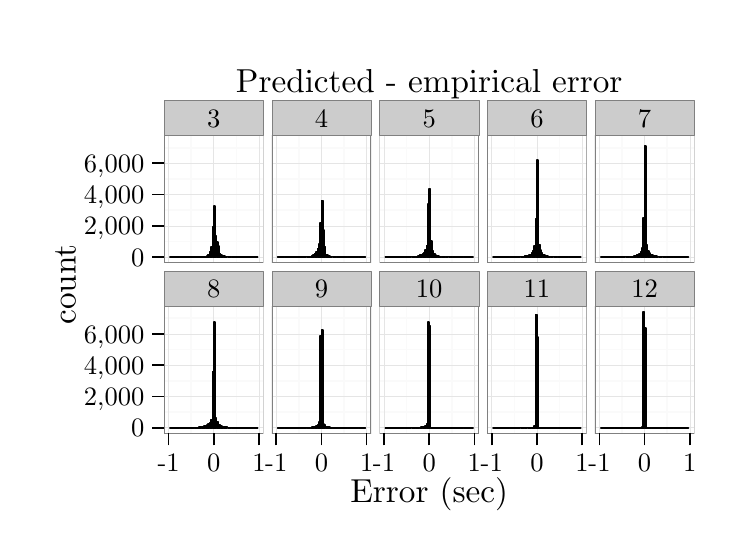
\begin{tikzpicture}[x=1pt,y=1pt]
\definecolor[named]{fillColor}{rgb}{1.00,1.00,1.00}
\path[use as bounding box,fill=fillColor,fill opacity=0.00] (0,0) rectangle (252.94,180.67);
\begin{scope}
\path[clip] (  0.00,  0.00) rectangle (252.94,180.67);
\definecolor[named]{drawColor}{rgb}{1.00,1.00,1.00}
\definecolor[named]{fillColor}{rgb}{1.00,1.00,1.00}

\path[draw=drawColor,line width= 0.6pt,line join=round,line cap=round,fill=fillColor] ( -0.00,  0.00) rectangle (252.95,180.67);
\end{scope}
\begin{scope}
\path[clip] ( 49.28, 95.69) rectangle ( 85.20,141.71);
\definecolor[named]{fillColor}{rgb}{1.00,1.00,1.00}

\path[fill=fillColor] ( 49.28, 95.69) rectangle ( 85.20,141.71);
\definecolor[named]{drawColor}{rgb}{0.98,0.98,0.98}

\path[draw=drawColor,line width= 0.6pt,line join=round] ( 49.28,103.43) --
	( 85.20,103.43);

\path[draw=drawColor,line width= 0.6pt,line join=round] ( 49.28,114.72) --
	( 85.20,114.72);

\path[draw=drawColor,line width= 0.6pt,line join=round] ( 49.28,126.01) --
	( 85.20,126.01);

\path[draw=drawColor,line width= 0.6pt,line join=round] ( 49.28,137.30) --
	( 85.20,137.30);

\path[draw=drawColor,line width= 0.6pt,line join=round] ( 59.08, 95.69) --
	( 59.08,141.71);

\path[draw=drawColor,line width= 0.6pt,line join=round] ( 75.40, 95.69) --
	( 75.40,141.71);
\definecolor[named]{drawColor}{rgb}{0.90,0.90,0.90}

\path[draw=drawColor,line width= 0.2pt,line join=round] ( 49.28, 97.79) --
	( 85.20, 97.79);

\path[draw=drawColor,line width= 0.2pt,line join=round] ( 49.28,109.07) --
	( 85.20,109.07);

\path[draw=drawColor,line width= 0.2pt,line join=round] ( 49.28,120.36) --
	( 85.20,120.36);

\path[draw=drawColor,line width= 0.2pt,line join=round] ( 49.28,131.65) --
	( 85.20,131.65);

\path[draw=drawColor,line width= 0.2pt,line join=round] ( 50.92, 95.69) --
	( 50.92,141.71);

\path[draw=drawColor,line width= 0.2pt,line join=round] ( 67.24, 95.69) --
	( 67.24,141.71);

\path[draw=drawColor,line width= 0.2pt,line join=round] ( 83.57, 95.69) --
	( 83.57,141.71);
\definecolor[named]{drawColor}{rgb}{0.00,0.00,0.00}
\definecolor[named]{fillColor}{rgb}{0.75,0.75,0.75}

\path[draw=drawColor,line width= 0.6pt,line join=round,fill=fillColor] ( 51.39, 97.79) rectangle ( 51.88, 97.79);

\path[draw=drawColor,line width= 0.6pt,line join=round,fill=fillColor] ( 51.88, 97.79) rectangle ( 52.38, 97.79);

\path[draw=drawColor,line width= 0.6pt,line join=round,fill=fillColor] ( 52.38, 97.79) rectangle ( 52.87, 97.79);

\path[draw=drawColor,line width= 0.6pt,line join=round,fill=fillColor] ( 52.87, 97.79) rectangle ( 53.37, 97.79);

\path[draw=drawColor,line width= 0.6pt,line join=round,fill=fillColor] ( 53.37, 97.79) rectangle ( 53.86, 97.79);

\path[draw=drawColor,line width= 0.6pt,line join=round,fill=fillColor] ( 53.86, 97.79) rectangle ( 54.36, 97.79);

\path[draw=drawColor,line width= 0.6pt,line join=round,fill=fillColor] ( 54.36, 97.79) rectangle ( 54.86, 97.79);

\path[draw=drawColor,line width= 0.6pt,line join=round,fill=fillColor] ( 54.86, 97.79) rectangle ( 55.35, 97.79);

\path[draw=drawColor,line width= 0.6pt,line join=round,fill=fillColor] ( 55.35, 97.79) rectangle ( 55.85, 97.79);

\path[draw=drawColor,line width= 0.6pt,line join=round,fill=fillColor] ( 55.85, 97.79) rectangle ( 56.34, 97.79);

\path[draw=drawColor,line width= 0.6pt,line join=round,fill=fillColor] ( 56.34, 97.79) rectangle ( 56.84, 97.79);

\path[draw=drawColor,line width= 0.6pt,line join=round,fill=fillColor] ( 56.84, 97.79) rectangle ( 57.33, 97.79);

\path[draw=drawColor,line width= 0.6pt,line join=round,fill=fillColor] ( 57.33, 97.79) rectangle ( 57.83, 97.79);

\path[draw=drawColor,line width= 0.6pt,line join=round,fill=fillColor] ( 57.83, 97.79) rectangle ( 58.32, 97.79);

\path[draw=drawColor,line width= 0.6pt,line join=round,fill=fillColor] ( 58.32, 97.79) rectangle ( 58.82, 97.79);

\path[draw=drawColor,line width= 0.6pt,line join=round,fill=fillColor] ( 58.82, 97.79) rectangle ( 59.31, 97.79);

\path[draw=drawColor,line width= 0.6pt,line join=round,fill=fillColor] ( 59.31, 97.79) rectangle ( 59.81, 97.79);

\path[draw=drawColor,line width= 0.6pt,line join=round,fill=fillColor] ( 59.81, 97.79) rectangle ( 60.31, 97.79);

\path[draw=drawColor,line width= 0.6pt,line join=round,fill=fillColor] ( 60.31, 97.79) rectangle ( 60.80, 97.79);

\path[draw=drawColor,line width= 0.6pt,line join=round,fill=fillColor] ( 60.80, 97.79) rectangle ( 61.30, 97.79);

\path[draw=drawColor,line width= 0.6pt,line join=round,fill=fillColor] ( 61.30, 97.79) rectangle ( 61.79, 97.79);

\path[draw=drawColor,line width= 0.6pt,line join=round,fill=fillColor] ( 61.79, 97.79) rectangle ( 62.29, 97.79);

\path[draw=drawColor,line width= 0.6pt,line join=round,fill=fillColor] ( 62.29, 97.79) rectangle ( 62.78, 97.79);

\path[draw=drawColor,line width= 0.6pt,line join=round,fill=fillColor] ( 62.78, 97.79) rectangle ( 63.28, 97.79);

\path[draw=drawColor,line width= 0.6pt,line join=round,fill=fillColor] ( 63.28, 97.79) rectangle ( 63.77, 97.79);

\path[draw=drawColor,line width= 0.6pt,line join=round,fill=fillColor] ( 63.77, 97.79) rectangle ( 64.27, 97.79);

\path[draw=drawColor,line width= 0.6pt,line join=round,fill=fillColor] ( 64.27, 97.79) rectangle ( 64.76, 97.79);

\path[draw=drawColor,line width= 0.6pt,line join=round,fill=fillColor] ( 64.76, 97.79) rectangle ( 65.26, 98.05);

\path[draw=drawColor,line width= 0.6pt,line join=round,fill=fillColor] ( 65.26, 97.79) rectangle ( 65.76, 98.75);

\path[draw=drawColor,line width= 0.6pt,line join=round,fill=fillColor] ( 65.76, 97.79) rectangle ( 66.25, 99.65);

\path[draw=drawColor,line width= 0.6pt,line join=round,fill=fillColor] ( 66.25, 97.79) rectangle ( 66.75,101.51);

\path[draw=drawColor,line width= 0.6pt,line join=round,fill=fillColor] ( 66.75, 97.79) rectangle ( 67.24,108.58);

\path[draw=drawColor,line width= 0.6pt,line join=round,fill=fillColor] ( 67.24, 97.79) rectangle ( 67.74,116.32);

\path[draw=drawColor,line width= 0.6pt,line join=round,fill=fillColor] ( 67.74, 97.79) rectangle ( 68.23,105.38);

\path[draw=drawColor,line width= 0.6pt,line join=round,fill=fillColor] ( 68.23, 97.79) rectangle ( 68.73,103.17);

\path[draw=drawColor,line width= 0.6pt,line join=round,fill=fillColor] ( 68.73, 97.79) rectangle ( 69.22,101.84);

\path[draw=drawColor,line width= 0.6pt,line join=round,fill=fillColor] ( 69.22, 97.79) rectangle ( 69.72, 99.09);

\path[draw=drawColor,line width= 0.6pt,line join=round,fill=fillColor] ( 69.72, 97.79) rectangle ( 70.21, 98.46);

\path[draw=drawColor,line width= 0.6pt,line join=round,fill=fillColor] ( 70.21, 97.79) rectangle ( 70.71, 98.11);

\path[draw=drawColor,line width= 0.6pt,line join=round,fill=fillColor] ( 70.71, 97.79) rectangle ( 71.20, 98.16);

\path[draw=drawColor,line width= 0.6pt,line join=round,fill=fillColor] ( 71.20, 97.79) rectangle ( 71.70, 97.96);

\path[draw=drawColor,line width= 0.6pt,line join=round,fill=fillColor] ( 71.70, 97.79) rectangle ( 72.20, 97.90);

\path[draw=drawColor,line width= 0.6pt,line join=round,fill=fillColor] ( 72.20, 97.79) rectangle ( 72.69, 97.84);

\path[draw=drawColor,line width= 0.6pt,line join=round,fill=fillColor] ( 72.69, 97.79) rectangle ( 73.19, 97.84);

\path[draw=drawColor,line width= 0.6pt,line join=round,fill=fillColor] ( 73.19, 97.79) rectangle ( 73.68, 97.84);

\path[draw=drawColor,line width= 0.6pt,line join=round,fill=fillColor] ( 73.68, 97.79) rectangle ( 74.18, 97.80);

\path[draw=drawColor,line width= 0.6pt,line join=round,fill=fillColor] ( 74.18, 97.79) rectangle ( 74.67, 97.83);

\path[draw=drawColor,line width= 0.6pt,line join=round,fill=fillColor] ( 74.67, 97.79) rectangle ( 75.17, 97.80);

\path[draw=drawColor,line width= 0.6pt,line join=round,fill=fillColor] ( 75.17, 97.79) rectangle ( 75.66, 97.80);

\path[draw=drawColor,line width= 0.6pt,line join=round,fill=fillColor] ( 75.66, 97.79) rectangle ( 76.16, 97.79);

\path[draw=drawColor,line width= 0.6pt,line join=round,fill=fillColor] ( 76.16, 97.79) rectangle ( 76.65, 97.79);

\path[draw=drawColor,line width= 0.6pt,line join=round,fill=fillColor] ( 76.65, 97.79) rectangle ( 77.15, 97.79);

\path[draw=drawColor,line width= 0.6pt,line join=round,fill=fillColor] ( 77.15, 97.79) rectangle ( 77.65, 97.79);

\path[draw=drawColor,line width= 0.6pt,line join=round,fill=fillColor] ( 77.65, 97.79) rectangle ( 78.14, 97.79);

\path[draw=drawColor,line width= 0.6pt,line join=round,fill=fillColor] ( 78.14, 97.79) rectangle ( 78.64, 97.79);

\path[draw=drawColor,line width= 0.6pt,line join=round,fill=fillColor] ( 78.64, 97.79) rectangle ( 79.13, 97.79);

\path[draw=drawColor,line width= 0.6pt,line join=round,fill=fillColor] ( 79.13, 97.79) rectangle ( 79.63, 97.79);

\path[draw=drawColor,line width= 0.6pt,line join=round,fill=fillColor] ( 79.63, 97.79) rectangle ( 80.12, 97.79);

\path[draw=drawColor,line width= 0.6pt,line join=round,fill=fillColor] ( 80.12, 97.79) rectangle ( 80.62, 97.79);

\path[draw=drawColor,line width= 0.6pt,line join=round,fill=fillColor] ( 80.62, 97.79) rectangle ( 81.11, 97.79);

\path[draw=drawColor,line width= 0.6pt,line join=round,fill=fillColor] ( 81.11, 97.79) rectangle ( 81.61, 97.79);

\path[draw=drawColor,line width= 0.6pt,line join=round,fill=fillColor] ( 81.61, 97.79) rectangle ( 82.10, 97.79);

\path[draw=drawColor,line width= 0.6pt,line join=round,fill=fillColor] ( 82.10, 97.79) rectangle ( 82.60, 97.79);

\path[draw=drawColor,line width= 0.6pt,line join=round,fill=fillColor] ( 82.60, 97.79) rectangle ( 83.10, 97.79);
\definecolor[named]{drawColor}{rgb}{0.50,0.50,0.50}

\path[draw=drawColor,line width= 0.6pt,line join=round,line cap=round] ( 49.28, 95.69) rectangle ( 85.20,141.71);
\end{scope}
\begin{scope}
\path[clip] ( 88.21, 95.69) rectangle (124.12,141.71);
\definecolor[named]{fillColor}{rgb}{1.00,1.00,1.00}

\path[fill=fillColor] ( 88.21, 95.69) rectangle (124.12,141.71);
\definecolor[named]{drawColor}{rgb}{0.98,0.98,0.98}

\path[draw=drawColor,line width= 0.6pt,line join=round] ( 88.21,103.43) --
	(124.12,103.43);

\path[draw=drawColor,line width= 0.6pt,line join=round] ( 88.21,114.72) --
	(124.12,114.72);

\path[draw=drawColor,line width= 0.6pt,line join=round] ( 88.21,126.01) --
	(124.12,126.01);

\path[draw=drawColor,line width= 0.6pt,line join=round] ( 88.21,137.30) --
	(124.12,137.30);

\path[draw=drawColor,line width= 0.6pt,line join=round] ( 98.00, 95.69) --
	( 98.00,141.71);

\path[draw=drawColor,line width= 0.6pt,line join=round] (114.33, 95.69) --
	(114.33,141.71);
\definecolor[named]{drawColor}{rgb}{0.90,0.90,0.90}

\path[draw=drawColor,line width= 0.2pt,line join=round] ( 88.21, 97.79) --
	(124.12, 97.79);

\path[draw=drawColor,line width= 0.2pt,line join=round] ( 88.21,109.07) --
	(124.12,109.07);

\path[draw=drawColor,line width= 0.2pt,line join=round] ( 88.21,120.36) --
	(124.12,120.36);

\path[draw=drawColor,line width= 0.2pt,line join=round] ( 88.21,131.65) --
	(124.12,131.65);

\path[draw=drawColor,line width= 0.2pt,line join=round] ( 89.84, 95.69) --
	( 89.84,141.71);

\path[draw=drawColor,line width= 0.2pt,line join=round] (106.17, 95.69) --
	(106.17,141.71);

\path[draw=drawColor,line width= 0.2pt,line join=round] (122.49, 95.69) --
	(122.49,141.71);
\definecolor[named]{drawColor}{rgb}{0.00,0.00,0.00}
\definecolor[named]{fillColor}{rgb}{0.75,0.75,0.75}

\path[draw=drawColor,line width= 0.6pt,line join=round,fill=fillColor] ( 90.31, 97.79) rectangle ( 90.81, 97.79);

\path[draw=drawColor,line width= 0.6pt,line join=round,fill=fillColor] ( 90.81, 97.79) rectangle ( 91.30, 97.79);

\path[draw=drawColor,line width= 0.6pt,line join=round,fill=fillColor] ( 91.30, 97.79) rectangle ( 91.80, 97.79);

\path[draw=drawColor,line width= 0.6pt,line join=round,fill=fillColor] ( 91.80, 97.79) rectangle ( 92.29, 97.79);

\path[draw=drawColor,line width= 0.6pt,line join=round,fill=fillColor] ( 92.29, 97.79) rectangle ( 92.79, 97.79);

\path[draw=drawColor,line width= 0.6pt,line join=round,fill=fillColor] ( 92.79, 97.79) rectangle ( 93.29, 97.79);

\path[draw=drawColor,line width= 0.6pt,line join=round,fill=fillColor] ( 93.29, 97.79) rectangle ( 93.78, 97.79);

\path[draw=drawColor,line width= 0.6pt,line join=round,fill=fillColor] ( 93.78, 97.79) rectangle ( 94.28, 97.79);

\path[draw=drawColor,line width= 0.6pt,line join=round,fill=fillColor] ( 94.28, 97.79) rectangle ( 94.77, 97.79);

\path[draw=drawColor,line width= 0.6pt,line join=round,fill=fillColor] ( 94.77, 97.79) rectangle ( 95.27, 97.79);

\path[draw=drawColor,line width= 0.6pt,line join=round,fill=fillColor] ( 95.27, 97.79) rectangle ( 95.76, 97.79);

\path[draw=drawColor,line width= 0.6pt,line join=round,fill=fillColor] ( 95.76, 97.79) rectangle ( 96.26, 97.79);

\path[draw=drawColor,line width= 0.6pt,line join=round,fill=fillColor] ( 96.26, 97.79) rectangle ( 96.75, 97.79);

\path[draw=drawColor,line width= 0.6pt,line join=round,fill=fillColor] ( 96.75, 97.79) rectangle ( 97.25, 97.79);

\path[draw=drawColor,line width= 0.6pt,line join=round,fill=fillColor] ( 97.25, 97.79) rectangle ( 97.74, 97.79);

\path[draw=drawColor,line width= 0.6pt,line join=round,fill=fillColor] ( 97.74, 97.79) rectangle ( 98.24, 97.79);

\path[draw=drawColor,line width= 0.6pt,line join=round,fill=fillColor] ( 98.24, 97.79) rectangle ( 98.74, 97.79);

\path[draw=drawColor,line width= 0.6pt,line join=round,fill=fillColor] ( 98.74, 97.79) rectangle ( 99.23, 97.79);

\path[draw=drawColor,line width= 0.6pt,line join=round,fill=fillColor] ( 99.23, 97.79) rectangle ( 99.73, 97.79);

\path[draw=drawColor,line width= 0.6pt,line join=round,fill=fillColor] ( 99.73, 97.79) rectangle (100.22, 97.79);

\path[draw=drawColor,line width= 0.6pt,line join=round,fill=fillColor] (100.22, 97.79) rectangle (100.72, 97.80);

\path[draw=drawColor,line width= 0.6pt,line join=round,fill=fillColor] (100.72, 97.79) rectangle (101.21, 97.80);

\path[draw=drawColor,line width= 0.6pt,line join=round,fill=fillColor] (101.21, 97.79) rectangle (101.71, 97.84);

\path[draw=drawColor,line width= 0.6pt,line join=round,fill=fillColor] (101.71, 97.79) rectangle (102.20, 97.96);

\path[draw=drawColor,line width= 0.6pt,line join=round,fill=fillColor] (102.20, 97.79) rectangle (102.70, 98.03);

\path[draw=drawColor,line width= 0.6pt,line join=round,fill=fillColor] (102.70, 97.79) rectangle (103.19, 98.31);

\path[draw=drawColor,line width= 0.6pt,line join=round,fill=fillColor] (103.19, 97.79) rectangle (103.69, 98.53);

\path[draw=drawColor,line width= 0.6pt,line join=round,fill=fillColor] (103.69, 97.79) rectangle (104.19, 99.03);

\path[draw=drawColor,line width= 0.6pt,line join=round,fill=fillColor] (104.19, 97.79) rectangle (104.68, 99.52);

\path[draw=drawColor,line width= 0.6pt,line join=round,fill=fillColor] (104.68, 97.79) rectangle (105.18,100.86);

\path[draw=drawColor,line width= 0.6pt,line join=round,fill=fillColor] (105.18, 97.79) rectangle (105.67,102.59);

\path[draw=drawColor,line width= 0.6pt,line join=round,fill=fillColor] (105.67, 97.79) rectangle (106.17,110.15);

\path[draw=drawColor,line width= 0.6pt,line join=round,fill=fillColor] (106.17, 97.79) rectangle (106.66,118.20);

\path[draw=drawColor,line width= 0.6pt,line join=round,fill=fillColor] (106.66, 97.79) rectangle (107.16,107.62);

\path[draw=drawColor,line width= 0.6pt,line join=round,fill=fillColor] (107.16, 97.79) rectangle (107.65,101.55);

\path[draw=drawColor,line width= 0.6pt,line join=round,fill=fillColor] (107.65, 97.79) rectangle (108.15, 98.66);

\path[draw=drawColor,line width= 0.6pt,line join=round,fill=fillColor] (108.15, 97.79) rectangle (108.64, 98.45);

\path[draw=drawColor,line width= 0.6pt,line join=round,fill=fillColor] (108.64, 97.79) rectangle (109.14, 98.14);

\path[draw=drawColor,line width= 0.6pt,line join=round,fill=fillColor] (109.14, 97.79) rectangle (109.63, 98.01);

\path[draw=drawColor,line width= 0.6pt,line join=round,fill=fillColor] (109.63, 97.79) rectangle (110.13, 97.90);

\path[draw=drawColor,line width= 0.6pt,line join=round,fill=fillColor] (110.13, 97.79) rectangle (110.63, 97.89);

\path[draw=drawColor,line width= 0.6pt,line join=round,fill=fillColor] (110.63, 97.79) rectangle (111.12, 97.85);

\path[draw=drawColor,line width= 0.6pt,line join=round,fill=fillColor] (111.12, 97.79) rectangle (111.62, 97.84);

\path[draw=drawColor,line width= 0.6pt,line join=round,fill=fillColor] (111.62, 97.79) rectangle (112.11, 97.80);

\path[draw=drawColor,line width= 0.6pt,line join=round,fill=fillColor] (112.11, 97.79) rectangle (112.61, 97.80);

\path[draw=drawColor,line width= 0.6pt,line join=round,fill=fillColor] (112.61, 97.79) rectangle (113.10, 97.79);

\path[draw=drawColor,line width= 0.6pt,line join=round,fill=fillColor] (113.10, 97.79) rectangle (113.60, 97.79);

\path[draw=drawColor,line width= 0.6pt,line join=round,fill=fillColor] (113.60, 97.79) rectangle (114.09, 97.80);

\path[draw=drawColor,line width= 0.6pt,line join=round,fill=fillColor] (114.09, 97.79) rectangle (114.59, 97.79);

\path[draw=drawColor,line width= 0.6pt,line join=round,fill=fillColor] (114.59, 97.79) rectangle (115.08, 97.79);

\path[draw=drawColor,line width= 0.6pt,line join=round,fill=fillColor] (115.08, 97.79) rectangle (115.58, 97.79);

\path[draw=drawColor,line width= 0.6pt,line join=round,fill=fillColor] (115.58, 97.79) rectangle (116.08, 97.79);

\path[draw=drawColor,line width= 0.6pt,line join=round,fill=fillColor] (116.08, 97.79) rectangle (116.57, 97.79);

\path[draw=drawColor,line width= 0.6pt,line join=round,fill=fillColor] (116.57, 97.79) rectangle (117.07, 97.79);

\path[draw=drawColor,line width= 0.6pt,line join=round,fill=fillColor] (117.07, 97.79) rectangle (117.56, 97.79);

\path[draw=drawColor,line width= 0.6pt,line join=round,fill=fillColor] (117.56, 97.79) rectangle (118.06, 97.79);

\path[draw=drawColor,line width= 0.6pt,line join=round,fill=fillColor] (118.06, 97.79) rectangle (118.55, 97.79);

\path[draw=drawColor,line width= 0.6pt,line join=round,fill=fillColor] (118.55, 97.79) rectangle (119.05, 97.79);

\path[draw=drawColor,line width= 0.6pt,line join=round,fill=fillColor] (119.05, 97.79) rectangle (119.54, 97.79);

\path[draw=drawColor,line width= 0.6pt,line join=round,fill=fillColor] (119.54, 97.79) rectangle (120.04, 97.79);

\path[draw=drawColor,line width= 0.6pt,line join=round,fill=fillColor] (120.04, 97.79) rectangle (120.53, 97.79);

\path[draw=drawColor,line width= 0.6pt,line join=round,fill=fillColor] (120.53, 97.79) rectangle (121.03, 97.79);

\path[draw=drawColor,line width= 0.6pt,line join=round,fill=fillColor] (121.03, 97.79) rectangle (121.53, 97.79);

\path[draw=drawColor,line width= 0.6pt,line join=round,fill=fillColor] (121.53, 97.79) rectangle (122.02, 97.79);
\definecolor[named]{drawColor}{rgb}{0.50,0.50,0.50}

\path[draw=drawColor,line width= 0.6pt,line join=round,line cap=round] ( 88.21, 95.69) rectangle (124.12,141.71);
\end{scope}
\begin{scope}
\path[clip] (127.14, 95.69) rectangle (163.05,141.71);
\definecolor[named]{fillColor}{rgb}{1.00,1.00,1.00}

\path[fill=fillColor] (127.14, 95.69) rectangle (163.05,141.71);
\definecolor[named]{drawColor}{rgb}{0.98,0.98,0.98}

\path[draw=drawColor,line width= 0.6pt,line join=round] (127.14,103.43) --
	(163.05,103.43);

\path[draw=drawColor,line width= 0.6pt,line join=round] (127.14,114.72) --
	(163.05,114.72);

\path[draw=drawColor,line width= 0.6pt,line join=round] (127.14,126.01) --
	(163.05,126.01);

\path[draw=drawColor,line width= 0.6pt,line join=round] (127.14,137.30) --
	(163.05,137.30);

\path[draw=drawColor,line width= 0.6pt,line join=round] (136.93, 95.69) --
	(136.93,141.71);

\path[draw=drawColor,line width= 0.6pt,line join=round] (153.25, 95.69) --
	(153.25,141.71);
\definecolor[named]{drawColor}{rgb}{0.90,0.90,0.90}

\path[draw=drawColor,line width= 0.2pt,line join=round] (127.14, 97.79) --
	(163.05, 97.79);

\path[draw=drawColor,line width= 0.2pt,line join=round] (127.14,109.07) --
	(163.05,109.07);

\path[draw=drawColor,line width= 0.2pt,line join=round] (127.14,120.36) --
	(163.05,120.36);

\path[draw=drawColor,line width= 0.2pt,line join=round] (127.14,131.65) --
	(163.05,131.65);

\path[draw=drawColor,line width= 0.2pt,line join=round] (128.77, 95.69) --
	(128.77,141.71);

\path[draw=drawColor,line width= 0.2pt,line join=round] (145.09, 95.69) --
	(145.09,141.71);

\path[draw=drawColor,line width= 0.2pt,line join=round] (161.42, 95.69) --
	(161.42,141.71);
\definecolor[named]{drawColor}{rgb}{0.00,0.00,0.00}
\definecolor[named]{fillColor}{rgb}{0.75,0.75,0.75}

\path[draw=drawColor,line width= 0.6pt,line join=round,fill=fillColor] (129.24, 97.79) rectangle (129.73, 97.79);

\path[draw=drawColor,line width= 0.6pt,line join=round,fill=fillColor] (129.73, 97.79) rectangle (130.23, 97.79);

\path[draw=drawColor,line width= 0.6pt,line join=round,fill=fillColor] (130.23, 97.79) rectangle (130.72, 97.79);

\path[draw=drawColor,line width= 0.6pt,line join=round,fill=fillColor] (130.72, 97.79) rectangle (131.22, 97.79);

\path[draw=drawColor,line width= 0.6pt,line join=round,fill=fillColor] (131.22, 97.79) rectangle (131.72, 97.79);

\path[draw=drawColor,line width= 0.6pt,line join=round,fill=fillColor] (131.72, 97.79) rectangle (132.21, 97.79);

\path[draw=drawColor,line width= 0.6pt,line join=round,fill=fillColor] (132.21, 97.79) rectangle (132.71, 97.79);

\path[draw=drawColor,line width= 0.6pt,line join=round,fill=fillColor] (132.71, 97.79) rectangle (133.20, 97.79);

\path[draw=drawColor,line width= 0.6pt,line join=round,fill=fillColor] (133.20, 97.79) rectangle (133.70, 97.79);

\path[draw=drawColor,line width= 0.6pt,line join=round,fill=fillColor] (133.70, 97.79) rectangle (134.19, 97.79);

\path[draw=drawColor,line width= 0.6pt,line join=round,fill=fillColor] (134.19, 97.79) rectangle (134.69, 97.79);

\path[draw=drawColor,line width= 0.6pt,line join=round,fill=fillColor] (134.69, 97.79) rectangle (135.18, 97.79);

\path[draw=drawColor,line width= 0.6pt,line join=round,fill=fillColor] (135.18, 97.79) rectangle (135.68, 97.79);

\path[draw=drawColor,line width= 0.6pt,line join=round,fill=fillColor] (135.68, 97.79) rectangle (136.17, 97.79);

\path[draw=drawColor,line width= 0.6pt,line join=round,fill=fillColor] (136.17, 97.79) rectangle (136.67, 97.79);

\path[draw=drawColor,line width= 0.6pt,line join=round,fill=fillColor] (136.67, 97.79) rectangle (137.17, 97.79);

\path[draw=drawColor,line width= 0.6pt,line join=round,fill=fillColor] (137.17, 97.79) rectangle (137.66, 97.79);

\path[draw=drawColor,line width= 0.6pt,line join=round,fill=fillColor] (137.66, 97.79) rectangle (138.16, 97.79);

\path[draw=drawColor,line width= 0.6pt,line join=round,fill=fillColor] (138.16, 97.79) rectangle (138.65, 97.80);

\path[draw=drawColor,line width= 0.6pt,line join=round,fill=fillColor] (138.65, 97.79) rectangle (139.15, 97.81);

\path[draw=drawColor,line width= 0.6pt,line join=round,fill=fillColor] (139.15, 97.79) rectangle (139.64, 97.83);

\path[draw=drawColor,line width= 0.6pt,line join=round,fill=fillColor] (139.64, 97.79) rectangle (140.14, 97.93);

\path[draw=drawColor,line width= 0.6pt,line join=round,fill=fillColor] (140.14, 97.79) rectangle (140.63, 97.97);

\path[draw=drawColor,line width= 0.6pt,line join=round,fill=fillColor] (140.63, 97.79) rectangle (141.13, 97.99);

\path[draw=drawColor,line width= 0.6pt,line join=round,fill=fillColor] (141.13, 97.79) rectangle (141.62, 98.28);

\path[draw=drawColor,line width= 0.6pt,line join=round,fill=fillColor] (141.62, 97.79) rectangle (142.12, 98.45);

\path[draw=drawColor,line width= 0.6pt,line join=round,fill=fillColor] (142.12, 97.79) rectangle (142.61, 98.46);

\path[draw=drawColor,line width= 0.6pt,line join=round,fill=fillColor] (142.61, 97.79) rectangle (143.11, 98.97);

\path[draw=drawColor,line width= 0.6pt,line join=round,fill=fillColor] (143.11, 97.79) rectangle (143.61, 99.44);

\path[draw=drawColor,line width= 0.6pt,line join=round,fill=fillColor] (143.61, 97.79) rectangle (144.10,100.43);

\path[draw=drawColor,line width= 0.6pt,line join=round,fill=fillColor] (144.10, 97.79) rectangle (144.60,101.96);

\path[draw=drawColor,line width= 0.6pt,line join=round,fill=fillColor] (144.60, 97.79) rectangle (145.09,116.89);

\path[draw=drawColor,line width= 0.6pt,line join=round,fill=fillColor] (145.09, 97.79) rectangle (145.59,122.31);

\path[draw=drawColor,line width= 0.6pt,line join=round,fill=fillColor] (145.59, 97.79) rectangle (146.08,103.50);

\path[draw=drawColor,line width= 0.6pt,line join=round,fill=fillColor] (146.08, 97.79) rectangle (146.58,100.17);

\path[draw=drawColor,line width= 0.6pt,line join=round,fill=fillColor] (146.58, 97.79) rectangle (147.07, 99.05);

\path[draw=drawColor,line width= 0.6pt,line join=round,fill=fillColor] (147.07, 97.79) rectangle (147.57, 98.53);

\path[draw=drawColor,line width= 0.6pt,line join=round,fill=fillColor] (147.57, 97.79) rectangle (148.06, 98.38);

\path[draw=drawColor,line width= 0.6pt,line join=round,fill=fillColor] (148.06, 97.79) rectangle (148.56, 98.09);

\path[draw=drawColor,line width= 0.6pt,line join=round,fill=fillColor] (148.56, 97.79) rectangle (149.06, 98.03);

\path[draw=drawColor,line width= 0.6pt,line join=round,fill=fillColor] (149.06, 97.79) rectangle (149.55, 97.92);

\path[draw=drawColor,line width= 0.6pt,line join=round,fill=fillColor] (149.55, 97.79) rectangle (150.05, 97.91);

\path[draw=drawColor,line width= 0.6pt,line join=round,fill=fillColor] (150.05, 97.79) rectangle (150.54, 97.86);

\path[draw=drawColor,line width= 0.6pt,line join=round,fill=fillColor] (150.54, 97.79) rectangle (151.04, 97.83);

\path[draw=drawColor,line width= 0.6pt,line join=round,fill=fillColor] (151.04, 97.79) rectangle (151.53, 97.83);

\path[draw=drawColor,line width= 0.6pt,line join=round,fill=fillColor] (151.53, 97.79) rectangle (152.03, 97.80);

\path[draw=drawColor,line width= 0.6pt,line join=round,fill=fillColor] (152.03, 97.79) rectangle (152.52, 97.80);

\path[draw=drawColor,line width= 0.6pt,line join=round,fill=fillColor] (152.52, 97.79) rectangle (153.02, 97.79);

\path[draw=drawColor,line width= 0.6pt,line join=round,fill=fillColor] (153.02, 97.79) rectangle (153.51, 97.80);

\path[draw=drawColor,line width= 0.6pt,line join=round,fill=fillColor] (153.51, 97.79) rectangle (154.01, 97.79);

\path[draw=drawColor,line width= 0.6pt,line join=round,fill=fillColor] (154.01, 97.79) rectangle (154.51, 97.79);

\path[draw=drawColor,line width= 0.6pt,line join=round,fill=fillColor] (154.51, 97.79) rectangle (155.00, 97.79);

\path[draw=drawColor,line width= 0.6pt,line join=round,fill=fillColor] (155.00, 97.79) rectangle (155.50, 97.79);

\path[draw=drawColor,line width= 0.6pt,line join=round,fill=fillColor] (155.50, 97.79) rectangle (155.99, 97.79);

\path[draw=drawColor,line width= 0.6pt,line join=round,fill=fillColor] (155.99, 97.79) rectangle (156.49, 97.79);

\path[draw=drawColor,line width= 0.6pt,line join=round,fill=fillColor] (156.49, 97.79) rectangle (156.98, 97.79);

\path[draw=drawColor,line width= 0.6pt,line join=round,fill=fillColor] (156.98, 97.79) rectangle (157.48, 97.79);

\path[draw=drawColor,line width= 0.6pt,line join=round,fill=fillColor] (157.48, 97.79) rectangle (157.97, 97.79);

\path[draw=drawColor,line width= 0.6pt,line join=round,fill=fillColor] (157.97, 97.79) rectangle (158.47, 97.79);

\path[draw=drawColor,line width= 0.6pt,line join=round,fill=fillColor] (158.47, 97.79) rectangle (158.96, 97.79);

\path[draw=drawColor,line width= 0.6pt,line join=round,fill=fillColor] (158.96, 97.79) rectangle (159.46, 97.79);

\path[draw=drawColor,line width= 0.6pt,line join=round,fill=fillColor] (159.46, 97.79) rectangle (159.96, 97.79);

\path[draw=drawColor,line width= 0.6pt,line join=round,fill=fillColor] (159.96, 97.79) rectangle (160.45, 97.79);

\path[draw=drawColor,line width= 0.6pt,line join=round,fill=fillColor] (160.45, 97.79) rectangle (160.95, 97.79);
\definecolor[named]{drawColor}{rgb}{0.50,0.50,0.50}

\path[draw=drawColor,line width= 0.6pt,line join=round,line cap=round] (127.14, 95.69) rectangle (163.05,141.71);
\end{scope}
\begin{scope}
\path[clip] (166.06, 95.69) rectangle (201.97,141.71);
\definecolor[named]{fillColor}{rgb}{1.00,1.00,1.00}

\path[fill=fillColor] (166.06, 95.69) rectangle (201.97,141.71);
\definecolor[named]{drawColor}{rgb}{0.98,0.98,0.98}

\path[draw=drawColor,line width= 0.6pt,line join=round] (166.06,103.43) --
	(201.97,103.43);

\path[draw=drawColor,line width= 0.6pt,line join=round] (166.06,114.72) --
	(201.97,114.72);

\path[draw=drawColor,line width= 0.6pt,line join=round] (166.06,126.01) --
	(201.97,126.01);

\path[draw=drawColor,line width= 0.6pt,line join=round] (166.06,137.30) --
	(201.97,137.30);

\path[draw=drawColor,line width= 0.6pt,line join=round] (175.86, 95.69) --
	(175.86,141.71);

\path[draw=drawColor,line width= 0.6pt,line join=round] (192.18, 95.69) --
	(192.18,141.71);
\definecolor[named]{drawColor}{rgb}{0.90,0.90,0.90}

\path[draw=drawColor,line width= 0.2pt,line join=round] (166.06, 97.79) --
	(201.97, 97.79);

\path[draw=drawColor,line width= 0.2pt,line join=round] (166.06,109.07) --
	(201.97,109.07);

\path[draw=drawColor,line width= 0.2pt,line join=round] (166.06,120.36) --
	(201.97,120.36);

\path[draw=drawColor,line width= 0.2pt,line join=round] (166.06,131.65) --
	(201.97,131.65);

\path[draw=drawColor,line width= 0.2pt,line join=round] (167.69, 95.69) --
	(167.69,141.71);

\path[draw=drawColor,line width= 0.2pt,line join=round] (184.02, 95.69) --
	(184.02,141.71);

\path[draw=drawColor,line width= 0.2pt,line join=round] (200.34, 95.69) --
	(200.34,141.71);
\definecolor[named]{drawColor}{rgb}{0.00,0.00,0.00}
\definecolor[named]{fillColor}{rgb}{0.75,0.75,0.75}

\path[draw=drawColor,line width= 0.6pt,line join=round,fill=fillColor] (168.16, 97.79) rectangle (168.66, 97.79);

\path[draw=drawColor,line width= 0.6pt,line join=round,fill=fillColor] (168.66, 97.79) rectangle (169.15, 97.79);

\path[draw=drawColor,line width= 0.6pt,line join=round,fill=fillColor] (169.15, 97.79) rectangle (169.65, 97.79);

\path[draw=drawColor,line width= 0.6pt,line join=round,fill=fillColor] (169.65, 97.79) rectangle (170.15, 97.79);

\path[draw=drawColor,line width= 0.6pt,line join=round,fill=fillColor] (170.15, 97.79) rectangle (170.64, 97.79);

\path[draw=drawColor,line width= 0.6pt,line join=round,fill=fillColor] (170.64, 97.79) rectangle (171.14, 97.79);

\path[draw=drawColor,line width= 0.6pt,line join=round,fill=fillColor] (171.14, 97.79) rectangle (171.63, 97.79);

\path[draw=drawColor,line width= 0.6pt,line join=round,fill=fillColor] (171.63, 97.79) rectangle (172.13, 97.79);

\path[draw=drawColor,line width= 0.6pt,line join=round,fill=fillColor] (172.13, 97.79) rectangle (172.62, 97.79);

\path[draw=drawColor,line width= 0.6pt,line join=round,fill=fillColor] (172.62, 97.79) rectangle (173.12, 97.79);

\path[draw=drawColor,line width= 0.6pt,line join=round,fill=fillColor] (173.12, 97.79) rectangle (173.61, 97.79);

\path[draw=drawColor,line width= 0.6pt,line join=round,fill=fillColor] (173.61, 97.79) rectangle (174.11, 97.79);

\path[draw=drawColor,line width= 0.6pt,line join=round,fill=fillColor] (174.11, 97.79) rectangle (174.60, 97.79);

\path[draw=drawColor,line width= 0.6pt,line join=round,fill=fillColor] (174.60, 97.79) rectangle (175.10, 97.79);

\path[draw=drawColor,line width= 0.6pt,line join=round,fill=fillColor] (175.10, 97.79) rectangle (175.60, 97.79);

\path[draw=drawColor,line width= 0.6pt,line join=round,fill=fillColor] (175.60, 97.79) rectangle (176.09, 97.79);

\path[draw=drawColor,line width= 0.6pt,line join=round,fill=fillColor] (176.09, 97.79) rectangle (176.59, 97.79);

\path[draw=drawColor,line width= 0.6pt,line join=round,fill=fillColor] (176.59, 97.79) rectangle (177.08, 97.79);

\path[draw=drawColor,line width= 0.6pt,line join=round,fill=fillColor] (177.08, 97.79) rectangle (177.58, 97.81);

\path[draw=drawColor,line width= 0.6pt,line join=round,fill=fillColor] (177.58, 97.79) rectangle (178.07, 97.81);

\path[draw=drawColor,line width= 0.6pt,line join=round,fill=fillColor] (178.07, 97.79) rectangle (178.57, 97.85);

\path[draw=drawColor,line width= 0.6pt,line join=round,fill=fillColor] (178.57, 97.79) rectangle (179.06, 97.92);

\path[draw=drawColor,line width= 0.6pt,line join=round,fill=fillColor] (179.06, 97.79) rectangle (179.56, 98.03);

\path[draw=drawColor,line width= 0.6pt,line join=round,fill=fillColor] (179.56, 97.79) rectangle (180.05, 98.07);

\path[draw=drawColor,line width= 0.6pt,line join=round,fill=fillColor] (180.05, 97.79) rectangle (180.55, 98.14);

\path[draw=drawColor,line width= 0.6pt,line join=round,fill=fillColor] (180.55, 97.79) rectangle (181.04, 98.31);

\path[draw=drawColor,line width= 0.6pt,line join=round,fill=fillColor] (181.04, 97.79) rectangle (181.54, 98.47);

\path[draw=drawColor,line width= 0.6pt,line join=round,fill=fillColor] (181.54, 97.79) rectangle (182.04, 98.75);

\path[draw=drawColor,line width= 0.6pt,line join=round,fill=fillColor] (182.04, 97.79) rectangle (182.53, 99.35);

\path[draw=drawColor,line width= 0.6pt,line join=round,fill=fillColor] (182.53, 97.79) rectangle (183.03,100.19);

\path[draw=drawColor,line width= 0.6pt,line join=round,fill=fillColor] (183.03, 97.79) rectangle (183.52,101.77);

\path[draw=drawColor,line width= 0.6pt,line join=round,fill=fillColor] (183.52, 97.79) rectangle (184.02,111.61);

\path[draw=drawColor,line width= 0.6pt,line join=round,fill=fillColor] (184.02, 97.79) rectangle (184.51,132.78);

\path[draw=drawColor,line width= 0.6pt,line join=round,fill=fillColor] (184.51, 97.79) rectangle (185.01,102.36);

\path[draw=drawColor,line width= 0.6pt,line join=round,fill=fillColor] (185.01, 97.79) rectangle (185.50,100.31);

\path[draw=drawColor,line width= 0.6pt,line join=round,fill=fillColor] (185.50, 97.79) rectangle (186.00, 99.36);

\path[draw=drawColor,line width= 0.6pt,line join=round,fill=fillColor] (186.00, 97.79) rectangle (186.49, 98.69);

\path[draw=drawColor,line width= 0.6pt,line join=round,fill=fillColor] (186.49, 97.79) rectangle (186.99, 98.44);

\path[draw=drawColor,line width= 0.6pt,line join=round,fill=fillColor] (186.99, 97.79) rectangle (187.49, 98.16);

\path[draw=drawColor,line width= 0.6pt,line join=round,fill=fillColor] (187.49, 97.79) rectangle (187.98, 98.18);

\path[draw=drawColor,line width= 0.6pt,line join=round,fill=fillColor] (187.98, 97.79) rectangle (188.48, 98.02);

\path[draw=drawColor,line width= 0.6pt,line join=round,fill=fillColor] (188.48, 97.79) rectangle (188.97, 98.01);

\path[draw=drawColor,line width= 0.6pt,line join=round,fill=fillColor] (188.97, 97.79) rectangle (189.47, 97.91);

\path[draw=drawColor,line width= 0.6pt,line join=round,fill=fillColor] (189.47, 97.79) rectangle (189.96, 97.87);

\path[draw=drawColor,line width= 0.6pt,line join=round,fill=fillColor] (189.96, 97.79) rectangle (190.46, 97.85);

\path[draw=drawColor,line width= 0.6pt,line join=round,fill=fillColor] (190.46, 97.79) rectangle (190.95, 97.82);

\path[draw=drawColor,line width= 0.6pt,line join=round,fill=fillColor] (190.95, 97.79) rectangle (191.45, 97.82);

\path[draw=drawColor,line width= 0.6pt,line join=round,fill=fillColor] (191.45, 97.79) rectangle (191.94, 97.80);

\path[draw=drawColor,line width= 0.6pt,line join=round,fill=fillColor] (191.94, 97.79) rectangle (192.44, 97.79);

\path[draw=drawColor,line width= 0.6pt,line join=round,fill=fillColor] (192.44, 97.79) rectangle (192.94, 97.79);

\path[draw=drawColor,line width= 0.6pt,line join=round,fill=fillColor] (192.94, 97.79) rectangle (193.43, 97.79);

\path[draw=drawColor,line width= 0.6pt,line join=round,fill=fillColor] (193.43, 97.79) rectangle (193.93, 97.79);

\path[draw=drawColor,line width= 0.6pt,line join=round,fill=fillColor] (193.93, 97.79) rectangle (194.42, 97.79);

\path[draw=drawColor,line width= 0.6pt,line join=round,fill=fillColor] (194.42, 97.79) rectangle (194.92, 97.79);

\path[draw=drawColor,line width= 0.6pt,line join=round,fill=fillColor] (194.92, 97.79) rectangle (195.41, 97.79);

\path[draw=drawColor,line width= 0.6pt,line join=round,fill=fillColor] (195.41, 97.79) rectangle (195.91, 97.79);

\path[draw=drawColor,line width= 0.6pt,line join=round,fill=fillColor] (195.91, 97.79) rectangle (196.40, 97.79);

\path[draw=drawColor,line width= 0.6pt,line join=round,fill=fillColor] (196.40, 97.79) rectangle (196.90, 97.79);

\path[draw=drawColor,line width= 0.6pt,line join=round,fill=fillColor] (196.90, 97.79) rectangle (197.39, 97.79);

\path[draw=drawColor,line width= 0.6pt,line join=round,fill=fillColor] (197.39, 97.79) rectangle (197.89, 97.79);

\path[draw=drawColor,line width= 0.6pt,line join=round,fill=fillColor] (197.89, 97.79) rectangle (198.39, 97.79);

\path[draw=drawColor,line width= 0.6pt,line join=round,fill=fillColor] (198.39, 97.79) rectangle (198.88, 97.79);

\path[draw=drawColor,line width= 0.6pt,line join=round,fill=fillColor] (198.88, 97.79) rectangle (199.38, 97.79);

\path[draw=drawColor,line width= 0.6pt,line join=round,fill=fillColor] (199.38, 97.79) rectangle (199.87, 97.79);
\definecolor[named]{drawColor}{rgb}{0.50,0.50,0.50}

\path[draw=drawColor,line width= 0.6pt,line join=round,line cap=round] (166.06, 95.69) rectangle (201.97,141.71);
\end{scope}
\begin{scope}
\path[clip] (204.99, 95.69) rectangle (240.90,141.71);
\definecolor[named]{fillColor}{rgb}{1.00,1.00,1.00}

\path[fill=fillColor] (204.99, 95.69) rectangle (240.90,141.71);
\definecolor[named]{drawColor}{rgb}{0.98,0.98,0.98}

\path[draw=drawColor,line width= 0.6pt,line join=round] (204.99,103.43) --
	(240.90,103.43);

\path[draw=drawColor,line width= 0.6pt,line join=round] (204.99,114.72) --
	(240.90,114.72);

\path[draw=drawColor,line width= 0.6pt,line join=round] (204.99,126.01) --
	(240.90,126.01);

\path[draw=drawColor,line width= 0.6pt,line join=round] (204.99,137.30) --
	(240.90,137.30);

\path[draw=drawColor,line width= 0.6pt,line join=round] (214.78, 95.69) --
	(214.78,141.71);

\path[draw=drawColor,line width= 0.6pt,line join=round] (231.11, 95.69) --
	(231.11,141.71);
\definecolor[named]{drawColor}{rgb}{0.90,0.90,0.90}

\path[draw=drawColor,line width= 0.2pt,line join=round] (204.99, 97.79) --
	(240.90, 97.79);

\path[draw=drawColor,line width= 0.2pt,line join=round] (204.99,109.07) --
	(240.90,109.07);

\path[draw=drawColor,line width= 0.2pt,line join=round] (204.99,120.36) --
	(240.90,120.36);

\path[draw=drawColor,line width= 0.2pt,line join=round] (204.99,131.65) --
	(240.90,131.65);

\path[draw=drawColor,line width= 0.2pt,line join=round] (206.62, 95.69) --
	(206.62,141.71);

\path[draw=drawColor,line width= 0.2pt,line join=round] (222.94, 95.69) --
	(222.94,141.71);

\path[draw=drawColor,line width= 0.2pt,line join=round] (239.27, 95.69) --
	(239.27,141.71);
\definecolor[named]{drawColor}{rgb}{0.00,0.00,0.00}
\definecolor[named]{fillColor}{rgb}{0.75,0.75,0.75}

\path[draw=drawColor,line width= 0.6pt,line join=round,fill=fillColor] (207.09, 97.79) rectangle (207.58, 97.79);

\path[draw=drawColor,line width= 0.6pt,line join=round,fill=fillColor] (207.58, 97.79) rectangle (208.08, 97.79);

\path[draw=drawColor,line width= 0.6pt,line join=round,fill=fillColor] (208.08, 97.79) rectangle (208.58, 97.79);

\path[draw=drawColor,line width= 0.6pt,line join=round,fill=fillColor] (208.58, 97.79) rectangle (209.07, 97.79);

\path[draw=drawColor,line width= 0.6pt,line join=round,fill=fillColor] (209.07, 97.79) rectangle (209.57, 97.79);

\path[draw=drawColor,line width= 0.6pt,line join=round,fill=fillColor] (209.57, 97.79) rectangle (210.06, 97.79);

\path[draw=drawColor,line width= 0.6pt,line join=round,fill=fillColor] (210.06, 97.79) rectangle (210.56, 97.79);

\path[draw=drawColor,line width= 0.6pt,line join=round,fill=fillColor] (210.56, 97.79) rectangle (211.05, 97.79);

\path[draw=drawColor,line width= 0.6pt,line join=round,fill=fillColor] (211.05, 97.79) rectangle (211.55, 97.79);

\path[draw=drawColor,line width= 0.6pt,line join=round,fill=fillColor] (211.55, 97.79) rectangle (212.04, 97.79);

\path[draw=drawColor,line width= 0.6pt,line join=round,fill=fillColor] (212.04, 97.79) rectangle (212.54, 97.79);

\path[draw=drawColor,line width= 0.6pt,line join=round,fill=fillColor] (212.54, 97.79) rectangle (213.03, 97.79);

\path[draw=drawColor,line width= 0.6pt,line join=round,fill=fillColor] (213.03, 97.79) rectangle (213.53, 97.79);

\path[draw=drawColor,line width= 0.6pt,line join=round,fill=fillColor] (213.53, 97.79) rectangle (214.03, 97.79);

\path[draw=drawColor,line width= 0.6pt,line join=round,fill=fillColor] (214.03, 97.79) rectangle (214.52, 97.80);

\path[draw=drawColor,line width= 0.6pt,line join=round,fill=fillColor] (214.52, 97.79) rectangle (215.02, 97.79);

\path[draw=drawColor,line width= 0.6pt,line join=round,fill=fillColor] (215.02, 97.79) rectangle (215.51, 97.80);

\path[draw=drawColor,line width= 0.6pt,line join=round,fill=fillColor] (215.51, 97.79) rectangle (216.01, 97.81);

\path[draw=drawColor,line width= 0.6pt,line join=round,fill=fillColor] (216.01, 97.79) rectangle (216.50, 97.84);

\path[draw=drawColor,line width= 0.6pt,line join=round,fill=fillColor] (216.50, 97.79) rectangle (217.00, 97.84);

\path[draw=drawColor,line width= 0.6pt,line join=round,fill=fillColor] (217.00, 97.79) rectangle (217.49, 97.90);

\path[draw=drawColor,line width= 0.6pt,line join=round,fill=fillColor] (217.49, 97.79) rectangle (217.99, 97.88);

\path[draw=drawColor,line width= 0.6pt,line join=round,fill=fillColor] (217.99, 97.79) rectangle (218.48, 98.01);

\path[draw=drawColor,line width= 0.6pt,line join=round,fill=fillColor] (218.48, 97.79) rectangle (218.98, 98.03);

\path[draw=drawColor,line width= 0.6pt,line join=round,fill=fillColor] (218.98, 97.79) rectangle (219.47, 98.05);

\path[draw=drawColor,line width= 0.6pt,line join=round,fill=fillColor] (219.47, 97.79) rectangle (219.97, 98.19);

\path[draw=drawColor,line width= 0.6pt,line join=round,fill=fillColor] (219.97, 97.79) rectangle (220.47, 98.43);

\path[draw=drawColor,line width= 0.6pt,line join=round,fill=fillColor] (220.47, 97.79) rectangle (220.96, 98.66);

\path[draw=drawColor,line width= 0.6pt,line join=round,fill=fillColor] (220.96, 97.79) rectangle (221.46, 99.00);

\path[draw=drawColor,line width= 0.6pt,line join=round,fill=fillColor] (221.46, 97.79) rectangle (221.95, 99.54);

\path[draw=drawColor,line width= 0.6pt,line join=round,fill=fillColor] (221.95, 97.79) rectangle (222.45,101.07);

\path[draw=drawColor,line width= 0.6pt,line join=round,fill=fillColor] (222.45, 97.79) rectangle (222.94,111.93);

\path[draw=drawColor,line width= 0.6pt,line join=round,fill=fillColor] (222.94, 97.79) rectangle (223.44,137.83);

\path[draw=drawColor,line width= 0.6pt,line join=round,fill=fillColor] (223.44, 97.79) rectangle (223.93,102.06);

\path[draw=drawColor,line width= 0.6pt,line join=round,fill=fillColor] (223.93, 97.79) rectangle (224.43, 99.98);

\path[draw=drawColor,line width= 0.6pt,line join=round,fill=fillColor] (224.43, 97.79) rectangle (224.92, 99.16);

\path[draw=drawColor,line width= 0.6pt,line join=round,fill=fillColor] (224.92, 97.79) rectangle (225.42, 98.72);

\path[draw=drawColor,line width= 0.6pt,line join=round,fill=fillColor] (225.42, 97.79) rectangle (225.92, 98.52);

\path[draw=drawColor,line width= 0.6pt,line join=round,fill=fillColor] (225.92, 97.79) rectangle (226.41, 98.23);

\path[draw=drawColor,line width= 0.6pt,line join=round,fill=fillColor] (226.41, 97.79) rectangle (226.91, 98.21);

\path[draw=drawColor,line width= 0.6pt,line join=round,fill=fillColor] (226.91, 97.79) rectangle (227.40, 98.07);

\path[draw=drawColor,line width= 0.6pt,line join=round,fill=fillColor] (227.40, 97.79) rectangle (227.90, 97.98);

\path[draw=drawColor,line width= 0.6pt,line join=round,fill=fillColor] (227.90, 97.79) rectangle (228.39, 97.89);

\path[draw=drawColor,line width= 0.6pt,line join=round,fill=fillColor] (228.39, 97.79) rectangle (228.89, 97.91);

\path[draw=drawColor,line width= 0.6pt,line join=round,fill=fillColor] (228.89, 97.79) rectangle (229.38, 97.84);

\path[draw=drawColor,line width= 0.6pt,line join=round,fill=fillColor] (229.38, 97.79) rectangle (229.88, 97.82);

\path[draw=drawColor,line width= 0.6pt,line join=round,fill=fillColor] (229.88, 97.79) rectangle (230.37, 97.81);

\path[draw=drawColor,line width= 0.6pt,line join=round,fill=fillColor] (230.37, 97.79) rectangle (230.87, 97.82);

\path[draw=drawColor,line width= 0.6pt,line join=round,fill=fillColor] (230.87, 97.79) rectangle (231.37, 97.80);

\path[draw=drawColor,line width= 0.6pt,line join=round,fill=fillColor] (231.37, 97.79) rectangle (231.86, 97.79);

\path[draw=drawColor,line width= 0.6pt,line join=round,fill=fillColor] (231.86, 97.79) rectangle (232.36, 97.79);

\path[draw=drawColor,line width= 0.6pt,line join=round,fill=fillColor] (232.36, 97.79) rectangle (232.85, 97.79);

\path[draw=drawColor,line width= 0.6pt,line join=round,fill=fillColor] (232.85, 97.79) rectangle (233.35, 97.79);

\path[draw=drawColor,line width= 0.6pt,line join=round,fill=fillColor] (233.35, 97.79) rectangle (233.84, 97.79);

\path[draw=drawColor,line width= 0.6pt,line join=round,fill=fillColor] (233.84, 97.79) rectangle (234.34, 97.79);

\path[draw=drawColor,line width= 0.6pt,line join=round,fill=fillColor] (234.34, 97.79) rectangle (234.83, 97.79);

\path[draw=drawColor,line width= 0.6pt,line join=round,fill=fillColor] (234.83, 97.79) rectangle (235.33, 97.79);

\path[draw=drawColor,line width= 0.6pt,line join=round,fill=fillColor] (235.33, 97.79) rectangle (235.82, 97.79);

\path[draw=drawColor,line width= 0.6pt,line join=round,fill=fillColor] (235.82, 97.79) rectangle (236.32, 97.79);

\path[draw=drawColor,line width= 0.6pt,line join=round,fill=fillColor] (236.32, 97.79) rectangle (236.82, 97.79);

\path[draw=drawColor,line width= 0.6pt,line join=round,fill=fillColor] (236.82, 97.79) rectangle (237.31, 97.79);

\path[draw=drawColor,line width= 0.6pt,line join=round,fill=fillColor] (237.31, 97.79) rectangle (237.81, 97.79);

\path[draw=drawColor,line width= 0.6pt,line join=round,fill=fillColor] (237.81, 97.79) rectangle (238.30, 97.79);

\path[draw=drawColor,line width= 0.6pt,line join=round,fill=fillColor] (238.30, 97.79) rectangle (238.80, 97.79);
\definecolor[named]{drawColor}{rgb}{0.50,0.50,0.50}

\path[draw=drawColor,line width= 0.6pt,line join=round,line cap=round] (204.99, 95.69) rectangle (240.90,141.71);
\end{scope}
\begin{scope}
\path[clip] ( 49.28, 34.03) rectangle ( 85.20, 80.05);
\definecolor[named]{fillColor}{rgb}{1.00,1.00,1.00}

\path[fill=fillColor] ( 49.28, 34.03) rectangle ( 85.20, 80.05);
\definecolor[named]{drawColor}{rgb}{0.98,0.98,0.98}

\path[draw=drawColor,line width= 0.6pt,line join=round] ( 49.28, 41.77) --
	( 85.20, 41.77);

\path[draw=drawColor,line width= 0.6pt,line join=round] ( 49.28, 53.06) --
	( 85.20, 53.06);

\path[draw=drawColor,line width= 0.6pt,line join=round] ( 49.28, 64.35) --
	( 85.20, 64.35);

\path[draw=drawColor,line width= 0.6pt,line join=round] ( 49.28, 75.64) --
	( 85.20, 75.64);

\path[draw=drawColor,line width= 0.6pt,line join=round] ( 59.08, 34.03) --
	( 59.08, 80.05);

\path[draw=drawColor,line width= 0.6pt,line join=round] ( 75.40, 34.03) --
	( 75.40, 80.05);
\definecolor[named]{drawColor}{rgb}{0.90,0.90,0.90}

\path[draw=drawColor,line width= 0.2pt,line join=round] ( 49.28, 36.13) --
	( 85.20, 36.13);

\path[draw=drawColor,line width= 0.2pt,line join=round] ( 49.28, 47.42) --
	( 85.20, 47.42);

\path[draw=drawColor,line width= 0.2pt,line join=round] ( 49.28, 58.70) --
	( 85.20, 58.70);

\path[draw=drawColor,line width= 0.2pt,line join=round] ( 49.28, 69.99) --
	( 85.20, 69.99);

\path[draw=drawColor,line width= 0.2pt,line join=round] ( 50.92, 34.03) --
	( 50.92, 80.05);

\path[draw=drawColor,line width= 0.2pt,line join=round] ( 67.24, 34.03) --
	( 67.24, 80.05);

\path[draw=drawColor,line width= 0.2pt,line join=round] ( 83.57, 34.03) --
	( 83.57, 80.05);
\definecolor[named]{drawColor}{rgb}{0.00,0.00,0.00}
\definecolor[named]{fillColor}{rgb}{0.75,0.75,0.75}

\path[draw=drawColor,line width= 0.6pt,line join=round,fill=fillColor] ( 51.39, 36.13) rectangle ( 51.88, 36.13);

\path[draw=drawColor,line width= 0.6pt,line join=round,fill=fillColor] ( 51.88, 36.13) rectangle ( 52.38, 36.13);

\path[draw=drawColor,line width= 0.6pt,line join=round,fill=fillColor] ( 52.38, 36.13) rectangle ( 52.87, 36.13);

\path[draw=drawColor,line width= 0.6pt,line join=round,fill=fillColor] ( 52.87, 36.13) rectangle ( 53.37, 36.13);

\path[draw=drawColor,line width= 0.6pt,line join=round,fill=fillColor] ( 53.37, 36.13) rectangle ( 53.86, 36.13);

\path[draw=drawColor,line width= 0.6pt,line join=round,fill=fillColor] ( 53.86, 36.13) rectangle ( 54.36, 36.13);

\path[draw=drawColor,line width= 0.6pt,line join=round,fill=fillColor] ( 54.36, 36.13) rectangle ( 54.86, 36.13);

\path[draw=drawColor,line width= 0.6pt,line join=round,fill=fillColor] ( 54.86, 36.13) rectangle ( 55.35, 36.13);

\path[draw=drawColor,line width= 0.6pt,line join=round,fill=fillColor] ( 55.35, 36.13) rectangle ( 55.85, 36.13);

\path[draw=drawColor,line width= 0.6pt,line join=round,fill=fillColor] ( 55.85, 36.13) rectangle ( 56.34, 36.13);

\path[draw=drawColor,line width= 0.6pt,line join=round,fill=fillColor] ( 56.34, 36.13) rectangle ( 56.84, 36.13);

\path[draw=drawColor,line width= 0.6pt,line join=round,fill=fillColor] ( 56.84, 36.13) rectangle ( 57.33, 36.13);

\path[draw=drawColor,line width= 0.6pt,line join=round,fill=fillColor] ( 57.33, 36.13) rectangle ( 57.83, 36.13);

\path[draw=drawColor,line width= 0.6pt,line join=round,fill=fillColor] ( 57.83, 36.13) rectangle ( 58.32, 36.13);

\path[draw=drawColor,line width= 0.6pt,line join=round,fill=fillColor] ( 58.32, 36.13) rectangle ( 58.82, 36.13);

\path[draw=drawColor,line width= 0.6pt,line join=round,fill=fillColor] ( 58.82, 36.13) rectangle ( 59.31, 36.13);

\path[draw=drawColor,line width= 0.6pt,line join=round,fill=fillColor] ( 59.31, 36.13) rectangle ( 59.81, 36.16);

\path[draw=drawColor,line width= 0.6pt,line join=round,fill=fillColor] ( 59.81, 36.13) rectangle ( 60.31, 36.18);

\path[draw=drawColor,line width= 0.6pt,line join=round,fill=fillColor] ( 60.31, 36.13) rectangle ( 60.80, 36.19);

\path[draw=drawColor,line width= 0.6pt,line join=round,fill=fillColor] ( 60.80, 36.13) rectangle ( 61.30, 36.20);

\path[draw=drawColor,line width= 0.6pt,line join=round,fill=fillColor] ( 61.30, 36.13) rectangle ( 61.79, 36.19);

\path[draw=drawColor,line width= 0.6pt,line join=round,fill=fillColor] ( 61.79, 36.13) rectangle ( 62.29, 36.27);

\path[draw=drawColor,line width= 0.6pt,line join=round,fill=fillColor] ( 62.29, 36.13) rectangle ( 62.78, 36.32);

\path[draw=drawColor,line width= 0.6pt,line join=round,fill=fillColor] ( 62.78, 36.13) rectangle ( 63.28, 36.40);

\path[draw=drawColor,line width= 0.6pt,line join=round,fill=fillColor] ( 63.28, 36.13) rectangle ( 63.77, 36.51);

\path[draw=drawColor,line width= 0.6pt,line join=round,fill=fillColor] ( 63.77, 36.13) rectangle ( 64.27, 36.66);

\path[draw=drawColor,line width= 0.6pt,line join=round,fill=fillColor] ( 64.27, 36.13) rectangle ( 64.76, 36.74);

\path[draw=drawColor,line width= 0.6pt,line join=round,fill=fillColor] ( 64.76, 36.13) rectangle ( 65.26, 37.11);

\path[draw=drawColor,line width= 0.6pt,line join=round,fill=fillColor] ( 65.26, 36.13) rectangle ( 65.76, 37.38);

\path[draw=drawColor,line width= 0.6pt,line join=round,fill=fillColor] ( 65.76, 36.13) rectangle ( 66.25, 37.75);

\path[draw=drawColor,line width= 0.6pt,line join=round,fill=fillColor] ( 66.25, 36.13) rectangle ( 66.75, 39.10);

\path[draw=drawColor,line width= 0.6pt,line join=round,fill=fillColor] ( 66.75, 36.13) rectangle ( 67.24, 56.46);

\path[draw=drawColor,line width= 0.6pt,line join=round,fill=fillColor] ( 67.24, 36.13) rectangle ( 67.74, 74.36);

\path[draw=drawColor,line width= 0.6pt,line join=round,fill=fillColor] ( 67.74, 36.13) rectangle ( 68.23, 39.54);

\path[draw=drawColor,line width= 0.6pt,line join=round,fill=fillColor] ( 68.23, 36.13) rectangle ( 68.73, 38.37);

\path[draw=drawColor,line width= 0.6pt,line join=round,fill=fillColor] ( 68.73, 36.13) rectangle ( 69.22, 37.21);

\path[draw=drawColor,line width= 0.6pt,line join=round,fill=fillColor] ( 69.22, 36.13) rectangle ( 69.72, 37.01);

\path[draw=drawColor,line width= 0.6pt,line join=round,fill=fillColor] ( 69.72, 36.13) rectangle ( 70.21, 36.75);

\path[draw=drawColor,line width= 0.6pt,line join=round,fill=fillColor] ( 70.21, 36.13) rectangle ( 70.71, 36.47);

\path[draw=drawColor,line width= 0.6pt,line join=round,fill=fillColor] ( 70.71, 36.13) rectangle ( 71.20, 36.39);

\path[draw=drawColor,line width= 0.6pt,line join=round,fill=fillColor] ( 71.20, 36.13) rectangle ( 71.70, 36.26);

\path[draw=drawColor,line width= 0.6pt,line join=round,fill=fillColor] ( 71.70, 36.13) rectangle ( 72.20, 36.26);

\path[draw=drawColor,line width= 0.6pt,line join=round,fill=fillColor] ( 72.20, 36.13) rectangle ( 72.69, 36.17);

\path[draw=drawColor,line width= 0.6pt,line join=round,fill=fillColor] ( 72.69, 36.13) rectangle ( 73.19, 36.17);

\path[draw=drawColor,line width= 0.6pt,line join=round,fill=fillColor] ( 73.19, 36.13) rectangle ( 73.68, 36.15);

\path[draw=drawColor,line width= 0.6pt,line join=round,fill=fillColor] ( 73.68, 36.13) rectangle ( 74.18, 36.14);

\path[draw=drawColor,line width= 0.6pt,line join=round,fill=fillColor] ( 74.18, 36.13) rectangle ( 74.67, 36.13);

\path[draw=drawColor,line width= 0.6pt,line join=round,fill=fillColor] ( 74.67, 36.13) rectangle ( 75.17, 36.13);

\path[draw=drawColor,line width= 0.6pt,line join=round,fill=fillColor] ( 75.17, 36.13) rectangle ( 75.66, 36.13);

\path[draw=drawColor,line width= 0.6pt,line join=round,fill=fillColor] ( 75.66, 36.13) rectangle ( 76.16, 36.13);

\path[draw=drawColor,line width= 0.6pt,line join=round,fill=fillColor] ( 76.16, 36.13) rectangle ( 76.65, 36.13);

\path[draw=drawColor,line width= 0.6pt,line join=round,fill=fillColor] ( 76.65, 36.13) rectangle ( 77.15, 36.13);

\path[draw=drawColor,line width= 0.6pt,line join=round,fill=fillColor] ( 77.15, 36.13) rectangle ( 77.65, 36.13);

\path[draw=drawColor,line width= 0.6pt,line join=round,fill=fillColor] ( 77.65, 36.13) rectangle ( 78.14, 36.13);

\path[draw=drawColor,line width= 0.6pt,line join=round,fill=fillColor] ( 78.14, 36.13) rectangle ( 78.64, 36.13);

\path[draw=drawColor,line width= 0.6pt,line join=round,fill=fillColor] ( 78.64, 36.13) rectangle ( 79.13, 36.13);

\path[draw=drawColor,line width= 0.6pt,line join=round,fill=fillColor] ( 79.13, 36.13) rectangle ( 79.63, 36.13);

\path[draw=drawColor,line width= 0.6pt,line join=round,fill=fillColor] ( 79.63, 36.13) rectangle ( 80.12, 36.13);

\path[draw=drawColor,line width= 0.6pt,line join=round,fill=fillColor] ( 80.12, 36.13) rectangle ( 80.62, 36.13);

\path[draw=drawColor,line width= 0.6pt,line join=round,fill=fillColor] ( 80.62, 36.13) rectangle ( 81.11, 36.13);

\path[draw=drawColor,line width= 0.6pt,line join=round,fill=fillColor] ( 81.11, 36.13) rectangle ( 81.61, 36.13);

\path[draw=drawColor,line width= 0.6pt,line join=round,fill=fillColor] ( 81.61, 36.13) rectangle ( 82.10, 36.13);

\path[draw=drawColor,line width= 0.6pt,line join=round,fill=fillColor] ( 82.10, 36.13) rectangle ( 82.60, 36.13);

\path[draw=drawColor,line width= 0.6pt,line join=round,fill=fillColor] ( 82.60, 36.13) rectangle ( 83.10, 36.13);
\definecolor[named]{drawColor}{rgb}{0.50,0.50,0.50}

\path[draw=drawColor,line width= 0.6pt,line join=round,line cap=round] ( 49.28, 34.03) rectangle ( 85.20, 80.05);
\end{scope}
\begin{scope}
\path[clip] ( 88.21, 34.03) rectangle (124.12, 80.05);
\definecolor[named]{fillColor}{rgb}{1.00,1.00,1.00}

\path[fill=fillColor] ( 88.21, 34.03) rectangle (124.12, 80.05);
\definecolor[named]{drawColor}{rgb}{0.98,0.98,0.98}

\path[draw=drawColor,line width= 0.6pt,line join=round] ( 88.21, 41.77) --
	(124.12, 41.77);

\path[draw=drawColor,line width= 0.6pt,line join=round] ( 88.21, 53.06) --
	(124.12, 53.06);

\path[draw=drawColor,line width= 0.6pt,line join=round] ( 88.21, 64.35) --
	(124.12, 64.35);

\path[draw=drawColor,line width= 0.6pt,line join=round] ( 88.21, 75.64) --
	(124.12, 75.64);

\path[draw=drawColor,line width= 0.6pt,line join=round] ( 98.00, 34.03) --
	( 98.00, 80.05);

\path[draw=drawColor,line width= 0.6pt,line join=round] (114.33, 34.03) --
	(114.33, 80.05);
\definecolor[named]{drawColor}{rgb}{0.90,0.90,0.90}

\path[draw=drawColor,line width= 0.2pt,line join=round] ( 88.21, 36.13) --
	(124.12, 36.13);

\path[draw=drawColor,line width= 0.2pt,line join=round] ( 88.21, 47.42) --
	(124.12, 47.42);

\path[draw=drawColor,line width= 0.2pt,line join=round] ( 88.21, 58.70) --
	(124.12, 58.70);

\path[draw=drawColor,line width= 0.2pt,line join=round] ( 88.21, 69.99) --
	(124.12, 69.99);

\path[draw=drawColor,line width= 0.2pt,line join=round] ( 89.84, 34.03) --
	( 89.84, 80.05);

\path[draw=drawColor,line width= 0.2pt,line join=round] (106.17, 34.03) --
	(106.17, 80.05);

\path[draw=drawColor,line width= 0.2pt,line join=round] (122.49, 34.03) --
	(122.49, 80.05);
\definecolor[named]{drawColor}{rgb}{0.00,0.00,0.00}
\definecolor[named]{fillColor}{rgb}{0.75,0.75,0.75}

\path[draw=drawColor,line width= 0.6pt,line join=round,fill=fillColor] ( 90.31, 36.13) rectangle ( 90.81, 36.13);

\path[draw=drawColor,line width= 0.6pt,line join=round,fill=fillColor] ( 90.81, 36.13) rectangle ( 91.30, 36.13);

\path[draw=drawColor,line width= 0.6pt,line join=round,fill=fillColor] ( 91.30, 36.13) rectangle ( 91.80, 36.13);

\path[draw=drawColor,line width= 0.6pt,line join=round,fill=fillColor] ( 91.80, 36.13) rectangle ( 92.29, 36.13);

\path[draw=drawColor,line width= 0.6pt,line join=round,fill=fillColor] ( 92.29, 36.13) rectangle ( 92.79, 36.13);

\path[draw=drawColor,line width= 0.6pt,line join=round,fill=fillColor] ( 92.79, 36.13) rectangle ( 93.29, 36.13);

\path[draw=drawColor,line width= 0.6pt,line join=round,fill=fillColor] ( 93.29, 36.13) rectangle ( 93.78, 36.13);

\path[draw=drawColor,line width= 0.6pt,line join=round,fill=fillColor] ( 93.78, 36.13) rectangle ( 94.28, 36.13);

\path[draw=drawColor,line width= 0.6pt,line join=round,fill=fillColor] ( 94.28, 36.13) rectangle ( 94.77, 36.13);

\path[draw=drawColor,line width= 0.6pt,line join=round,fill=fillColor] ( 94.77, 36.13) rectangle ( 95.27, 36.13);

\path[draw=drawColor,line width= 0.6pt,line join=round,fill=fillColor] ( 95.27, 36.13) rectangle ( 95.76, 36.13);

\path[draw=drawColor,line width= 0.6pt,line join=round,fill=fillColor] ( 95.76, 36.13) rectangle ( 96.26, 36.13);

\path[draw=drawColor,line width= 0.6pt,line join=round,fill=fillColor] ( 96.26, 36.13) rectangle ( 96.75, 36.13);

\path[draw=drawColor,line width= 0.6pt,line join=round,fill=fillColor] ( 96.75, 36.13) rectangle ( 97.25, 36.13);

\path[draw=drawColor,line width= 0.6pt,line join=round,fill=fillColor] ( 97.25, 36.13) rectangle ( 97.74, 36.13);

\path[draw=drawColor,line width= 0.6pt,line join=round,fill=fillColor] ( 97.74, 36.13) rectangle ( 98.24, 36.13);

\path[draw=drawColor,line width= 0.6pt,line join=round,fill=fillColor] ( 98.24, 36.13) rectangle ( 98.74, 36.13);

\path[draw=drawColor,line width= 0.6pt,line join=round,fill=fillColor] ( 98.74, 36.13) rectangle ( 99.23, 36.14);

\path[draw=drawColor,line width= 0.6pt,line join=round,fill=fillColor] ( 99.23, 36.13) rectangle ( 99.73, 36.16);

\path[draw=drawColor,line width= 0.6pt,line join=round,fill=fillColor] ( 99.73, 36.13) rectangle (100.22, 36.17);

\path[draw=drawColor,line width= 0.6pt,line join=round,fill=fillColor] (100.22, 36.13) rectangle (100.72, 36.19);

\path[draw=drawColor,line width= 0.6pt,line join=round,fill=fillColor] (100.72, 36.13) rectangle (101.21, 36.21);

\path[draw=drawColor,line width= 0.6pt,line join=round,fill=fillColor] (101.21, 36.13) rectangle (101.71, 36.23);

\path[draw=drawColor,line width= 0.6pt,line join=round,fill=fillColor] (101.71, 36.13) rectangle (102.20, 36.21);

\path[draw=drawColor,line width= 0.6pt,line join=round,fill=fillColor] (102.20, 36.13) rectangle (102.70, 36.24);

\path[draw=drawColor,line width= 0.6pt,line join=round,fill=fillColor] (102.70, 36.13) rectangle (103.19, 36.27);

\path[draw=drawColor,line width= 0.6pt,line join=round,fill=fillColor] (103.19, 36.13) rectangle (103.69, 36.44);

\path[draw=drawColor,line width= 0.6pt,line join=round,fill=fillColor] (103.69, 36.13) rectangle (104.19, 36.59);

\path[draw=drawColor,line width= 0.6pt,line join=round,fill=fillColor] (104.19, 36.13) rectangle (104.68, 36.82);

\path[draw=drawColor,line width= 0.6pt,line join=round,fill=fillColor] (104.68, 36.13) rectangle (105.18, 37.16);

\path[draw=drawColor,line width= 0.6pt,line join=round,fill=fillColor] (105.18, 36.13) rectangle (105.67, 38.07);

\path[draw=drawColor,line width= 0.6pt,line join=round,fill=fillColor] (105.67, 36.13) rectangle (106.17, 69.24);

\path[draw=drawColor,line width= 0.6pt,line join=round,fill=fillColor] (106.17, 36.13) rectangle (106.66, 71.49);

\path[draw=drawColor,line width= 0.6pt,line join=round,fill=fillColor] (106.66, 36.13) rectangle (107.16, 37.55);

\path[draw=drawColor,line width= 0.6pt,line join=round,fill=fillColor] (107.16, 36.13) rectangle (107.65, 37.13);

\path[draw=drawColor,line width= 0.6pt,line join=round,fill=fillColor] (107.65, 36.13) rectangle (108.15, 36.60);

\path[draw=drawColor,line width= 0.6pt,line join=round,fill=fillColor] (108.15, 36.13) rectangle (108.64, 36.26);

\path[draw=drawColor,line width= 0.6pt,line join=round,fill=fillColor] (108.64, 36.13) rectangle (109.14, 36.26);

\path[draw=drawColor,line width= 0.6pt,line join=round,fill=fillColor] (109.14, 36.13) rectangle (109.63, 36.22);

\path[draw=drawColor,line width= 0.6pt,line join=round,fill=fillColor] (109.63, 36.13) rectangle (110.13, 36.13);

\path[draw=drawColor,line width= 0.6pt,line join=round,fill=fillColor] (110.13, 36.13) rectangle (110.63, 36.13);

\path[draw=drawColor,line width= 0.6pt,line join=round,fill=fillColor] (110.63, 36.13) rectangle (111.12, 36.13);

\path[draw=drawColor,line width= 0.6pt,line join=round,fill=fillColor] (111.12, 36.13) rectangle (111.62, 36.13);

\path[draw=drawColor,line width= 0.6pt,line join=round,fill=fillColor] (111.62, 36.13) rectangle (112.11, 36.13);

\path[draw=drawColor,line width= 0.6pt,line join=round,fill=fillColor] (112.11, 36.13) rectangle (112.61, 36.13);

\path[draw=drawColor,line width= 0.6pt,line join=round,fill=fillColor] (112.61, 36.13) rectangle (113.10, 36.13);

\path[draw=drawColor,line width= 0.6pt,line join=round,fill=fillColor] (113.10, 36.13) rectangle (113.60, 36.13);

\path[draw=drawColor,line width= 0.6pt,line join=round,fill=fillColor] (113.60, 36.13) rectangle (114.09, 36.13);

\path[draw=drawColor,line width= 0.6pt,line join=round,fill=fillColor] (114.09, 36.13) rectangle (114.59, 36.13);

\path[draw=drawColor,line width= 0.6pt,line join=round,fill=fillColor] (114.59, 36.13) rectangle (115.08, 36.13);

\path[draw=drawColor,line width= 0.6pt,line join=round,fill=fillColor] (115.08, 36.13) rectangle (115.58, 36.13);

\path[draw=drawColor,line width= 0.6pt,line join=round,fill=fillColor] (115.58, 36.13) rectangle (116.08, 36.13);

\path[draw=drawColor,line width= 0.6pt,line join=round,fill=fillColor] (116.08, 36.13) rectangle (116.57, 36.13);

\path[draw=drawColor,line width= 0.6pt,line join=round,fill=fillColor] (116.57, 36.13) rectangle (117.07, 36.13);

\path[draw=drawColor,line width= 0.6pt,line join=round,fill=fillColor] (117.07, 36.13) rectangle (117.56, 36.13);

\path[draw=drawColor,line width= 0.6pt,line join=round,fill=fillColor] (117.56, 36.13) rectangle (118.06, 36.13);

\path[draw=drawColor,line width= 0.6pt,line join=round,fill=fillColor] (118.06, 36.13) rectangle (118.55, 36.13);

\path[draw=drawColor,line width= 0.6pt,line join=round,fill=fillColor] (118.55, 36.13) rectangle (119.05, 36.13);

\path[draw=drawColor,line width= 0.6pt,line join=round,fill=fillColor] (119.05, 36.13) rectangle (119.54, 36.13);

\path[draw=drawColor,line width= 0.6pt,line join=round,fill=fillColor] (119.54, 36.13) rectangle (120.04, 36.13);

\path[draw=drawColor,line width= 0.6pt,line join=round,fill=fillColor] (120.04, 36.13) rectangle (120.53, 36.13);

\path[draw=drawColor,line width= 0.6pt,line join=round,fill=fillColor] (120.53, 36.13) rectangle (121.03, 36.13);

\path[draw=drawColor,line width= 0.6pt,line join=round,fill=fillColor] (121.03, 36.13) rectangle (121.53, 36.13);

\path[draw=drawColor,line width= 0.6pt,line join=round,fill=fillColor] (121.53, 36.13) rectangle (122.02, 36.13);
\definecolor[named]{drawColor}{rgb}{0.50,0.50,0.50}

\path[draw=drawColor,line width= 0.6pt,line join=round,line cap=round] ( 88.21, 34.03) rectangle (124.12, 80.05);
\end{scope}
\begin{scope}
\path[clip] (127.14, 34.03) rectangle (163.05, 80.05);
\definecolor[named]{fillColor}{rgb}{1.00,1.00,1.00}

\path[fill=fillColor] (127.14, 34.03) rectangle (163.05, 80.05);
\definecolor[named]{drawColor}{rgb}{0.98,0.98,0.98}

\path[draw=drawColor,line width= 0.6pt,line join=round] (127.14, 41.77) --
	(163.05, 41.77);

\path[draw=drawColor,line width= 0.6pt,line join=round] (127.14, 53.06) --
	(163.05, 53.06);

\path[draw=drawColor,line width= 0.6pt,line join=round] (127.14, 64.35) --
	(163.05, 64.35);

\path[draw=drawColor,line width= 0.6pt,line join=round] (127.14, 75.64) --
	(163.05, 75.64);

\path[draw=drawColor,line width= 0.6pt,line join=round] (136.93, 34.03) --
	(136.93, 80.05);

\path[draw=drawColor,line width= 0.6pt,line join=round] (153.25, 34.03) --
	(153.25, 80.05);
\definecolor[named]{drawColor}{rgb}{0.90,0.90,0.90}

\path[draw=drawColor,line width= 0.2pt,line join=round] (127.14, 36.13) --
	(163.05, 36.13);

\path[draw=drawColor,line width= 0.2pt,line join=round] (127.14, 47.42) --
	(163.05, 47.42);

\path[draw=drawColor,line width= 0.2pt,line join=round] (127.14, 58.70) --
	(163.05, 58.70);

\path[draw=drawColor,line width= 0.2pt,line join=round] (127.14, 69.99) --
	(163.05, 69.99);

\path[draw=drawColor,line width= 0.2pt,line join=round] (128.77, 34.03) --
	(128.77, 80.05);

\path[draw=drawColor,line width= 0.2pt,line join=round] (145.09, 34.03) --
	(145.09, 80.05);

\path[draw=drawColor,line width= 0.2pt,line join=round] (161.42, 34.03) --
	(161.42, 80.05);
\definecolor[named]{drawColor}{rgb}{0.00,0.00,0.00}
\definecolor[named]{fillColor}{rgb}{0.75,0.75,0.75}

\path[draw=drawColor,line width= 0.6pt,line join=round,fill=fillColor] (129.24, 36.13) rectangle (129.73, 36.13);

\path[draw=drawColor,line width= 0.6pt,line join=round,fill=fillColor] (129.73, 36.13) rectangle (130.23, 36.13);

\path[draw=drawColor,line width= 0.6pt,line join=round,fill=fillColor] (130.23, 36.13) rectangle (130.72, 36.13);

\path[draw=drawColor,line width= 0.6pt,line join=round,fill=fillColor] (130.72, 36.13) rectangle (131.22, 36.13);

\path[draw=drawColor,line width= 0.6pt,line join=round,fill=fillColor] (131.22, 36.13) rectangle (131.72, 36.13);

\path[draw=drawColor,line width= 0.6pt,line join=round,fill=fillColor] (131.72, 36.13) rectangle (132.21, 36.13);

\path[draw=drawColor,line width= 0.6pt,line join=round,fill=fillColor] (132.21, 36.13) rectangle (132.71, 36.13);

\path[draw=drawColor,line width= 0.6pt,line join=round,fill=fillColor] (132.71, 36.13) rectangle (133.20, 36.13);

\path[draw=drawColor,line width= 0.6pt,line join=round,fill=fillColor] (133.20, 36.13) rectangle (133.70, 36.13);

\path[draw=drawColor,line width= 0.6pt,line join=round,fill=fillColor] (133.70, 36.13) rectangle (134.19, 36.13);

\path[draw=drawColor,line width= 0.6pt,line join=round,fill=fillColor] (134.19, 36.13) rectangle (134.69, 36.13);

\path[draw=drawColor,line width= 0.6pt,line join=round,fill=fillColor] (134.69, 36.13) rectangle (135.18, 36.13);

\path[draw=drawColor,line width= 0.6pt,line join=round,fill=fillColor] (135.18, 36.13) rectangle (135.68, 36.13);

\path[draw=drawColor,line width= 0.6pt,line join=round,fill=fillColor] (135.68, 36.13) rectangle (136.17, 36.13);

\path[draw=drawColor,line width= 0.6pt,line join=round,fill=fillColor] (136.17, 36.13) rectangle (136.67, 36.13);

\path[draw=drawColor,line width= 0.6pt,line join=round,fill=fillColor] (136.67, 36.13) rectangle (137.17, 36.13);

\path[draw=drawColor,line width= 0.6pt,line join=round,fill=fillColor] (137.17, 36.13) rectangle (137.66, 36.13);

\path[draw=drawColor,line width= 0.6pt,line join=round,fill=fillColor] (137.66, 36.13) rectangle (138.16, 36.13);

\path[draw=drawColor,line width= 0.6pt,line join=round,fill=fillColor] (138.16, 36.13) rectangle (138.65, 36.14);

\path[draw=drawColor,line width= 0.6pt,line join=round,fill=fillColor] (138.65, 36.13) rectangle (139.15, 36.17);

\path[draw=drawColor,line width= 0.6pt,line join=round,fill=fillColor] (139.15, 36.13) rectangle (139.64, 36.14);

\path[draw=drawColor,line width= 0.6pt,line join=round,fill=fillColor] (139.64, 36.13) rectangle (140.14, 36.13);

\path[draw=drawColor,line width= 0.6pt,line join=round,fill=fillColor] (140.14, 36.13) rectangle (140.63, 36.15);

\path[draw=drawColor,line width= 0.6pt,line join=round,fill=fillColor] (140.63, 36.13) rectangle (141.13, 36.17);

\path[draw=drawColor,line width= 0.6pt,line join=round,fill=fillColor] (141.13, 36.13) rectangle (141.62, 36.22);

\path[draw=drawColor,line width= 0.6pt,line join=round,fill=fillColor] (141.62, 36.13) rectangle (142.12, 36.23);

\path[draw=drawColor,line width= 0.6pt,line join=round,fill=fillColor] (142.12, 36.13) rectangle (142.61, 36.31);

\path[draw=drawColor,line width= 0.6pt,line join=round,fill=fillColor] (142.61, 36.13) rectangle (143.11, 36.35);

\path[draw=drawColor,line width= 0.6pt,line join=round,fill=fillColor] (143.11, 36.13) rectangle (143.61, 36.54);

\path[draw=drawColor,line width= 0.6pt,line join=round,fill=fillColor] (143.61, 36.13) rectangle (144.10, 36.71);

\path[draw=drawColor,line width= 0.6pt,line join=round,fill=fillColor] (144.10, 36.13) rectangle (144.60, 37.44);

\path[draw=drawColor,line width= 0.6pt,line join=round,fill=fillColor] (144.60, 36.13) rectangle (145.09, 74.33);

\path[draw=drawColor,line width= 0.6pt,line join=round,fill=fillColor] (145.09, 36.13) rectangle (145.59, 72.78);

\path[draw=drawColor,line width= 0.6pt,line join=round,fill=fillColor] (145.59, 36.13) rectangle (146.08, 36.13);

\path[draw=drawColor,line width= 0.6pt,line join=round,fill=fillColor] (146.08, 36.13) rectangle (146.58, 36.13);

\path[draw=drawColor,line width= 0.6pt,line join=round,fill=fillColor] (146.58, 36.13) rectangle (147.07, 36.13);

\path[draw=drawColor,line width= 0.6pt,line join=round,fill=fillColor] (147.07, 36.13) rectangle (147.57, 36.13);

\path[draw=drawColor,line width= 0.6pt,line join=round,fill=fillColor] (147.57, 36.13) rectangle (148.06, 36.13);

\path[draw=drawColor,line width= 0.6pt,line join=round,fill=fillColor] (148.06, 36.13) rectangle (148.56, 36.13);

\path[draw=drawColor,line width= 0.6pt,line join=round,fill=fillColor] (148.56, 36.13) rectangle (149.06, 36.13);

\path[draw=drawColor,line width= 0.6pt,line join=round,fill=fillColor] (149.06, 36.13) rectangle (149.55, 36.13);

\path[draw=drawColor,line width= 0.6pt,line join=round,fill=fillColor] (149.55, 36.13) rectangle (150.05, 36.13);

\path[draw=drawColor,line width= 0.6pt,line join=round,fill=fillColor] (150.05, 36.13) rectangle (150.54, 36.13);

\path[draw=drawColor,line width= 0.6pt,line join=round,fill=fillColor] (150.54, 36.13) rectangle (151.04, 36.13);

\path[draw=drawColor,line width= 0.6pt,line join=round,fill=fillColor] (151.04, 36.13) rectangle (151.53, 36.13);

\path[draw=drawColor,line width= 0.6pt,line join=round,fill=fillColor] (151.53, 36.13) rectangle (152.03, 36.13);

\path[draw=drawColor,line width= 0.6pt,line join=round,fill=fillColor] (152.03, 36.13) rectangle (152.52, 36.13);

\path[draw=drawColor,line width= 0.6pt,line join=round,fill=fillColor] (152.52, 36.13) rectangle (153.02, 36.13);

\path[draw=drawColor,line width= 0.6pt,line join=round,fill=fillColor] (153.02, 36.13) rectangle (153.51, 36.13);

\path[draw=drawColor,line width= 0.6pt,line join=round,fill=fillColor] (153.51, 36.13) rectangle (154.01, 36.13);

\path[draw=drawColor,line width= 0.6pt,line join=round,fill=fillColor] (154.01, 36.13) rectangle (154.51, 36.13);

\path[draw=drawColor,line width= 0.6pt,line join=round,fill=fillColor] (154.51, 36.13) rectangle (155.00, 36.13);

\path[draw=drawColor,line width= 0.6pt,line join=round,fill=fillColor] (155.00, 36.13) rectangle (155.50, 36.13);

\path[draw=drawColor,line width= 0.6pt,line join=round,fill=fillColor] (155.50, 36.13) rectangle (155.99, 36.13);

\path[draw=drawColor,line width= 0.6pt,line join=round,fill=fillColor] (155.99, 36.13) rectangle (156.49, 36.13);

\path[draw=drawColor,line width= 0.6pt,line join=round,fill=fillColor] (156.49, 36.13) rectangle (156.98, 36.13);

\path[draw=drawColor,line width= 0.6pt,line join=round,fill=fillColor] (156.98, 36.13) rectangle (157.48, 36.13);

\path[draw=drawColor,line width= 0.6pt,line join=round,fill=fillColor] (157.48, 36.13) rectangle (157.97, 36.13);

\path[draw=drawColor,line width= 0.6pt,line join=round,fill=fillColor] (157.97, 36.13) rectangle (158.47, 36.13);

\path[draw=drawColor,line width= 0.6pt,line join=round,fill=fillColor] (158.47, 36.13) rectangle (158.96, 36.13);

\path[draw=drawColor,line width= 0.6pt,line join=round,fill=fillColor] (158.96, 36.13) rectangle (159.46, 36.13);

\path[draw=drawColor,line width= 0.6pt,line join=round,fill=fillColor] (159.46, 36.13) rectangle (159.96, 36.13);

\path[draw=drawColor,line width= 0.6pt,line join=round,fill=fillColor] (159.96, 36.13) rectangle (160.45, 36.13);

\path[draw=drawColor,line width= 0.6pt,line join=round,fill=fillColor] (160.45, 36.13) rectangle (160.95, 36.13);
\definecolor[named]{drawColor}{rgb}{0.50,0.50,0.50}

\path[draw=drawColor,line width= 0.6pt,line join=round,line cap=round] (127.14, 34.03) rectangle (163.05, 80.05);
\end{scope}
\begin{scope}
\path[clip] (166.06, 34.03) rectangle (201.97, 80.05);
\definecolor[named]{fillColor}{rgb}{1.00,1.00,1.00}

\path[fill=fillColor] (166.06, 34.03) rectangle (201.97, 80.05);
\definecolor[named]{drawColor}{rgb}{0.98,0.98,0.98}

\path[draw=drawColor,line width= 0.6pt,line join=round] (166.06, 41.77) --
	(201.97, 41.77);

\path[draw=drawColor,line width= 0.6pt,line join=round] (166.06, 53.06) --
	(201.97, 53.06);

\path[draw=drawColor,line width= 0.6pt,line join=round] (166.06, 64.35) --
	(201.97, 64.35);

\path[draw=drawColor,line width= 0.6pt,line join=round] (166.06, 75.64) --
	(201.97, 75.64);

\path[draw=drawColor,line width= 0.6pt,line join=round] (175.86, 34.03) --
	(175.86, 80.05);

\path[draw=drawColor,line width= 0.6pt,line join=round] (192.18, 34.03) --
	(192.18, 80.05);
\definecolor[named]{drawColor}{rgb}{0.90,0.90,0.90}

\path[draw=drawColor,line width= 0.2pt,line join=round] (166.06, 36.13) --
	(201.97, 36.13);

\path[draw=drawColor,line width= 0.2pt,line join=round] (166.06, 47.42) --
	(201.97, 47.42);

\path[draw=drawColor,line width= 0.2pt,line join=round] (166.06, 58.70) --
	(201.97, 58.70);

\path[draw=drawColor,line width= 0.2pt,line join=round] (166.06, 69.99) --
	(201.97, 69.99);

\path[draw=drawColor,line width= 0.2pt,line join=round] (167.69, 34.03) --
	(167.69, 80.05);

\path[draw=drawColor,line width= 0.2pt,line join=round] (184.02, 34.03) --
	(184.02, 80.05);

\path[draw=drawColor,line width= 0.2pt,line join=round] (200.34, 34.03) --
	(200.34, 80.05);
\definecolor[named]{drawColor}{rgb}{0.00,0.00,0.00}
\definecolor[named]{fillColor}{rgb}{0.75,0.75,0.75}

\path[draw=drawColor,line width= 0.6pt,line join=round,fill=fillColor] (168.16, 36.13) rectangle (168.66, 36.13);

\path[draw=drawColor,line width= 0.6pt,line join=round,fill=fillColor] (168.66, 36.13) rectangle (169.15, 36.13);

\path[draw=drawColor,line width= 0.6pt,line join=round,fill=fillColor] (169.15, 36.13) rectangle (169.65, 36.13);

\path[draw=drawColor,line width= 0.6pt,line join=round,fill=fillColor] (169.65, 36.13) rectangle (170.15, 36.13);

\path[draw=drawColor,line width= 0.6pt,line join=round,fill=fillColor] (170.15, 36.13) rectangle (170.64, 36.13);

\path[draw=drawColor,line width= 0.6pt,line join=round,fill=fillColor] (170.64, 36.13) rectangle (171.14, 36.13);

\path[draw=drawColor,line width= 0.6pt,line join=round,fill=fillColor] (171.14, 36.13) rectangle (171.63, 36.13);

\path[draw=drawColor,line width= 0.6pt,line join=round,fill=fillColor] (171.63, 36.13) rectangle (172.13, 36.13);

\path[draw=drawColor,line width= 0.6pt,line join=round,fill=fillColor] (172.13, 36.13) rectangle (172.62, 36.13);

\path[draw=drawColor,line width= 0.6pt,line join=round,fill=fillColor] (172.62, 36.13) rectangle (173.12, 36.13);

\path[draw=drawColor,line width= 0.6pt,line join=round,fill=fillColor] (173.12, 36.13) rectangle (173.61, 36.13);

\path[draw=drawColor,line width= 0.6pt,line join=round,fill=fillColor] (173.61, 36.13) rectangle (174.11, 36.13);

\path[draw=drawColor,line width= 0.6pt,line join=round,fill=fillColor] (174.11, 36.13) rectangle (174.60, 36.13);

\path[draw=drawColor,line width= 0.6pt,line join=round,fill=fillColor] (174.60, 36.13) rectangle (175.10, 36.13);

\path[draw=drawColor,line width= 0.6pt,line join=round,fill=fillColor] (175.10, 36.13) rectangle (175.60, 36.13);

\path[draw=drawColor,line width= 0.6pt,line join=round,fill=fillColor] (175.60, 36.13) rectangle (176.09, 36.13);

\path[draw=drawColor,line width= 0.6pt,line join=round,fill=fillColor] (176.09, 36.13) rectangle (176.59, 36.13);

\path[draw=drawColor,line width= 0.6pt,line join=round,fill=fillColor] (176.59, 36.13) rectangle (177.08, 36.13);

\path[draw=drawColor,line width= 0.6pt,line join=round,fill=fillColor] (177.08, 36.13) rectangle (177.58, 36.13);

\path[draw=drawColor,line width= 0.6pt,line join=round,fill=fillColor] (177.58, 36.13) rectangle (178.07, 36.13);

\path[draw=drawColor,line width= 0.6pt,line join=round,fill=fillColor] (178.07, 36.13) rectangle (178.57, 36.14);

\path[draw=drawColor,line width= 0.6pt,line join=round,fill=fillColor] (178.57, 36.13) rectangle (179.06, 36.13);

\path[draw=drawColor,line width= 0.6pt,line join=round,fill=fillColor] (179.06, 36.13) rectangle (179.56, 36.15);

\path[draw=drawColor,line width= 0.6pt,line join=round,fill=fillColor] (179.56, 36.13) rectangle (180.05, 36.14);

\path[draw=drawColor,line width= 0.6pt,line join=round,fill=fillColor] (180.05, 36.13) rectangle (180.55, 36.15);

\path[draw=drawColor,line width= 0.6pt,line join=round,fill=fillColor] (180.55, 36.13) rectangle (181.04, 36.14);

\path[draw=drawColor,line width= 0.6pt,line join=round,fill=fillColor] (181.04, 36.13) rectangle (181.54, 36.16);

\path[draw=drawColor,line width= 0.6pt,line join=round,fill=fillColor] (181.54, 36.13) rectangle (182.04, 36.16);

\path[draw=drawColor,line width= 0.6pt,line join=round,fill=fillColor] (182.04, 36.13) rectangle (182.53, 36.24);

\path[draw=drawColor,line width= 0.6pt,line join=round,fill=fillColor] (182.53, 36.13) rectangle (183.03, 36.24);

\path[draw=drawColor,line width= 0.6pt,line join=round,fill=fillColor] (183.03, 36.13) rectangle (183.52, 36.66);

\path[draw=drawColor,line width= 0.6pt,line join=round,fill=fillColor] (183.52, 36.13) rectangle (184.02, 77.00);

\path[draw=drawColor,line width= 0.6pt,line join=round,fill=fillColor] (184.02, 36.13) rectangle (184.51, 68.85);

\path[draw=drawColor,line width= 0.6pt,line join=round,fill=fillColor] (184.51, 36.13) rectangle (185.01, 36.13);

\path[draw=drawColor,line width= 0.6pt,line join=round,fill=fillColor] (185.01, 36.13) rectangle (185.50, 36.13);

\path[draw=drawColor,line width= 0.6pt,line join=round,fill=fillColor] (185.50, 36.13) rectangle (186.00, 36.13);

\path[draw=drawColor,line width= 0.6pt,line join=round,fill=fillColor] (186.00, 36.13) rectangle (186.49, 36.13);

\path[draw=drawColor,line width= 0.6pt,line join=round,fill=fillColor] (186.49, 36.13) rectangle (186.99, 36.13);

\path[draw=drawColor,line width= 0.6pt,line join=round,fill=fillColor] (186.99, 36.13) rectangle (187.49, 36.13);

\path[draw=drawColor,line width= 0.6pt,line join=round,fill=fillColor] (187.49, 36.13) rectangle (187.98, 36.13);

\path[draw=drawColor,line width= 0.6pt,line join=round,fill=fillColor] (187.98, 36.13) rectangle (188.48, 36.13);

\path[draw=drawColor,line width= 0.6pt,line join=round,fill=fillColor] (188.48, 36.13) rectangle (188.97, 36.13);

\path[draw=drawColor,line width= 0.6pt,line join=round,fill=fillColor] (188.97, 36.13) rectangle (189.47, 36.13);

\path[draw=drawColor,line width= 0.6pt,line join=round,fill=fillColor] (189.47, 36.13) rectangle (189.96, 36.13);

\path[draw=drawColor,line width= 0.6pt,line join=round,fill=fillColor] (189.96, 36.13) rectangle (190.46, 36.13);

\path[draw=drawColor,line width= 0.6pt,line join=round,fill=fillColor] (190.46, 36.13) rectangle (190.95, 36.13);

\path[draw=drawColor,line width= 0.6pt,line join=round,fill=fillColor] (190.95, 36.13) rectangle (191.45, 36.13);

\path[draw=drawColor,line width= 0.6pt,line join=round,fill=fillColor] (191.45, 36.13) rectangle (191.94, 36.13);

\path[draw=drawColor,line width= 0.6pt,line join=round,fill=fillColor] (191.94, 36.13) rectangle (192.44, 36.13);

\path[draw=drawColor,line width= 0.6pt,line join=round,fill=fillColor] (192.44, 36.13) rectangle (192.94, 36.13);

\path[draw=drawColor,line width= 0.6pt,line join=round,fill=fillColor] (192.94, 36.13) rectangle (193.43, 36.13);

\path[draw=drawColor,line width= 0.6pt,line join=round,fill=fillColor] (193.43, 36.13) rectangle (193.93, 36.13);

\path[draw=drawColor,line width= 0.6pt,line join=round,fill=fillColor] (193.93, 36.13) rectangle (194.42, 36.13);

\path[draw=drawColor,line width= 0.6pt,line join=round,fill=fillColor] (194.42, 36.13) rectangle (194.92, 36.13);

\path[draw=drawColor,line width= 0.6pt,line join=round,fill=fillColor] (194.92, 36.13) rectangle (195.41, 36.13);

\path[draw=drawColor,line width= 0.6pt,line join=round,fill=fillColor] (195.41, 36.13) rectangle (195.91, 36.13);

\path[draw=drawColor,line width= 0.6pt,line join=round,fill=fillColor] (195.91, 36.13) rectangle (196.40, 36.13);

\path[draw=drawColor,line width= 0.6pt,line join=round,fill=fillColor] (196.40, 36.13) rectangle (196.90, 36.13);

\path[draw=drawColor,line width= 0.6pt,line join=round,fill=fillColor] (196.90, 36.13) rectangle (197.39, 36.13);

\path[draw=drawColor,line width= 0.6pt,line join=round,fill=fillColor] (197.39, 36.13) rectangle (197.89, 36.13);

\path[draw=drawColor,line width= 0.6pt,line join=round,fill=fillColor] (197.89, 36.13) rectangle (198.39, 36.13);

\path[draw=drawColor,line width= 0.6pt,line join=round,fill=fillColor] (198.39, 36.13) rectangle (198.88, 36.13);

\path[draw=drawColor,line width= 0.6pt,line join=round,fill=fillColor] (198.88, 36.13) rectangle (199.38, 36.13);

\path[draw=drawColor,line width= 0.6pt,line join=round,fill=fillColor] (199.38, 36.13) rectangle (199.87, 36.13);
\definecolor[named]{drawColor}{rgb}{0.50,0.50,0.50}

\path[draw=drawColor,line width= 0.6pt,line join=round,line cap=round] (166.06, 34.03) rectangle (201.97, 80.05);
\end{scope}
\begin{scope}
\path[clip] (204.99, 34.03) rectangle (240.90, 80.05);
\definecolor[named]{fillColor}{rgb}{1.00,1.00,1.00}

\path[fill=fillColor] (204.99, 34.03) rectangle (240.90, 80.05);
\definecolor[named]{drawColor}{rgb}{0.98,0.98,0.98}

\path[draw=drawColor,line width= 0.6pt,line join=round] (204.99, 41.77) --
	(240.90, 41.77);

\path[draw=drawColor,line width= 0.6pt,line join=round] (204.99, 53.06) --
	(240.90, 53.06);

\path[draw=drawColor,line width= 0.6pt,line join=round] (204.99, 64.35) --
	(240.90, 64.35);

\path[draw=drawColor,line width= 0.6pt,line join=round] (204.99, 75.64) --
	(240.90, 75.64);

\path[draw=drawColor,line width= 0.6pt,line join=round] (214.78, 34.03) --
	(214.78, 80.05);

\path[draw=drawColor,line width= 0.6pt,line join=round] (231.11, 34.03) --
	(231.11, 80.05);
\definecolor[named]{drawColor}{rgb}{0.90,0.90,0.90}

\path[draw=drawColor,line width= 0.2pt,line join=round] (204.99, 36.13) --
	(240.90, 36.13);

\path[draw=drawColor,line width= 0.2pt,line join=round] (204.99, 47.42) --
	(240.90, 47.42);

\path[draw=drawColor,line width= 0.2pt,line join=round] (204.99, 58.70) --
	(240.90, 58.70);

\path[draw=drawColor,line width= 0.2pt,line join=round] (204.99, 69.99) --
	(240.90, 69.99);

\path[draw=drawColor,line width= 0.2pt,line join=round] (206.62, 34.03) --
	(206.62, 80.05);

\path[draw=drawColor,line width= 0.2pt,line join=round] (222.94, 34.03) --
	(222.94, 80.05);

\path[draw=drawColor,line width= 0.2pt,line join=round] (239.27, 34.03) --
	(239.27, 80.05);
\definecolor[named]{drawColor}{rgb}{0.00,0.00,0.00}
\definecolor[named]{fillColor}{rgb}{0.75,0.75,0.75}

\path[draw=drawColor,line width= 0.6pt,line join=round,fill=fillColor] (207.09, 36.13) rectangle (207.58, 36.13);

\path[draw=drawColor,line width= 0.6pt,line join=round,fill=fillColor] (207.58, 36.13) rectangle (208.08, 36.13);

\path[draw=drawColor,line width= 0.6pt,line join=round,fill=fillColor] (208.08, 36.13) rectangle (208.58, 36.13);

\path[draw=drawColor,line width= 0.6pt,line join=round,fill=fillColor] (208.58, 36.13) rectangle (209.07, 36.13);

\path[draw=drawColor,line width= 0.6pt,line join=round,fill=fillColor] (209.07, 36.13) rectangle (209.57, 36.13);

\path[draw=drawColor,line width= 0.6pt,line join=round,fill=fillColor] (209.57, 36.13) rectangle (210.06, 36.13);

\path[draw=drawColor,line width= 0.6pt,line join=round,fill=fillColor] (210.06, 36.13) rectangle (210.56, 36.13);

\path[draw=drawColor,line width= 0.6pt,line join=round,fill=fillColor] (210.56, 36.13) rectangle (211.05, 36.13);

\path[draw=drawColor,line width= 0.6pt,line join=round,fill=fillColor] (211.05, 36.13) rectangle (211.55, 36.13);

\path[draw=drawColor,line width= 0.6pt,line join=round,fill=fillColor] (211.55, 36.13) rectangle (212.04, 36.13);

\path[draw=drawColor,line width= 0.6pt,line join=round,fill=fillColor] (212.04, 36.13) rectangle (212.54, 36.13);

\path[draw=drawColor,line width= 0.6pt,line join=round,fill=fillColor] (212.54, 36.13) rectangle (213.03, 36.13);

\path[draw=drawColor,line width= 0.6pt,line join=round,fill=fillColor] (213.03, 36.13) rectangle (213.53, 36.13);

\path[draw=drawColor,line width= 0.6pt,line join=round,fill=fillColor] (213.53, 36.13) rectangle (214.03, 36.13);

\path[draw=drawColor,line width= 0.6pt,line join=round,fill=fillColor] (214.03, 36.13) rectangle (214.52, 36.13);

\path[draw=drawColor,line width= 0.6pt,line join=round,fill=fillColor] (214.52, 36.13) rectangle (215.02, 36.13);

\path[draw=drawColor,line width= 0.6pt,line join=round,fill=fillColor] (215.02, 36.13) rectangle (215.51, 36.13);

\path[draw=drawColor,line width= 0.6pt,line join=round,fill=fillColor] (215.51, 36.13) rectangle (216.01, 36.13);

\path[draw=drawColor,line width= 0.6pt,line join=round,fill=fillColor] (216.01, 36.13) rectangle (216.50, 36.13);

\path[draw=drawColor,line width= 0.6pt,line join=round,fill=fillColor] (216.50, 36.13) rectangle (217.00, 36.13);

\path[draw=drawColor,line width= 0.6pt,line join=round,fill=fillColor] (217.00, 36.13) rectangle (217.49, 36.13);

\path[draw=drawColor,line width= 0.6pt,line join=round,fill=fillColor] (217.49, 36.13) rectangle (217.99, 36.13);

\path[draw=drawColor,line width= 0.6pt,line join=round,fill=fillColor] (217.99, 36.13) rectangle (218.48, 36.13);

\path[draw=drawColor,line width= 0.6pt,line join=round,fill=fillColor] (218.48, 36.13) rectangle (218.98, 36.13);

\path[draw=drawColor,line width= 0.6pt,line join=round,fill=fillColor] (218.98, 36.13) rectangle (219.47, 36.13);

\path[draw=drawColor,line width= 0.6pt,line join=round,fill=fillColor] (219.47, 36.13) rectangle (219.97, 36.13);

\path[draw=drawColor,line width= 0.6pt,line join=round,fill=fillColor] (219.97, 36.13) rectangle (220.47, 36.13);

\path[draw=drawColor,line width= 0.6pt,line join=round,fill=fillColor] (220.47, 36.13) rectangle (220.96, 36.13);

\path[draw=drawColor,line width= 0.6pt,line join=round,fill=fillColor] (220.96, 36.13) rectangle (221.46, 36.14);

\path[draw=drawColor,line width= 0.6pt,line join=round,fill=fillColor] (221.46, 36.13) rectangle (221.95, 36.15);

\path[draw=drawColor,line width= 0.6pt,line join=round,fill=fillColor] (221.95, 36.13) rectangle (222.45, 36.34);

\path[draw=drawColor,line width= 0.6pt,line join=round,fill=fillColor] (222.45, 36.13) rectangle (222.94, 77.96);

\path[draw=drawColor,line width= 0.6pt,line join=round,fill=fillColor] (222.94, 36.13) rectangle (223.44, 72.26);

\path[draw=drawColor,line width= 0.6pt,line join=round,fill=fillColor] (223.44, 36.13) rectangle (223.93, 36.13);

\path[draw=drawColor,line width= 0.6pt,line join=round,fill=fillColor] (223.93, 36.13) rectangle (224.43, 36.13);

\path[draw=drawColor,line width= 0.6pt,line join=round,fill=fillColor] (224.43, 36.13) rectangle (224.92, 36.13);

\path[draw=drawColor,line width= 0.6pt,line join=round,fill=fillColor] (224.92, 36.13) rectangle (225.42, 36.13);

\path[draw=drawColor,line width= 0.6pt,line join=round,fill=fillColor] (225.42, 36.13) rectangle (225.92, 36.13);

\path[draw=drawColor,line width= 0.6pt,line join=round,fill=fillColor] (225.92, 36.13) rectangle (226.41, 36.13);

\path[draw=drawColor,line width= 0.6pt,line join=round,fill=fillColor] (226.41, 36.13) rectangle (226.91, 36.13);

\path[draw=drawColor,line width= 0.6pt,line join=round,fill=fillColor] (226.91, 36.13) rectangle (227.40, 36.13);

\path[draw=drawColor,line width= 0.6pt,line join=round,fill=fillColor] (227.40, 36.13) rectangle (227.90, 36.13);

\path[draw=drawColor,line width= 0.6pt,line join=round,fill=fillColor] (227.90, 36.13) rectangle (228.39, 36.13);

\path[draw=drawColor,line width= 0.6pt,line join=round,fill=fillColor] (228.39, 36.13) rectangle (228.89, 36.13);

\path[draw=drawColor,line width= 0.6pt,line join=round,fill=fillColor] (228.89, 36.13) rectangle (229.38, 36.13);

\path[draw=drawColor,line width= 0.6pt,line join=round,fill=fillColor] (229.38, 36.13) rectangle (229.88, 36.13);

\path[draw=drawColor,line width= 0.6pt,line join=round,fill=fillColor] (229.88, 36.13) rectangle (230.37, 36.13);

\path[draw=drawColor,line width= 0.6pt,line join=round,fill=fillColor] (230.37, 36.13) rectangle (230.87, 36.13);

\path[draw=drawColor,line width= 0.6pt,line join=round,fill=fillColor] (230.87, 36.13) rectangle (231.37, 36.13);

\path[draw=drawColor,line width= 0.6pt,line join=round,fill=fillColor] (231.37, 36.13) rectangle (231.86, 36.13);

\path[draw=drawColor,line width= 0.6pt,line join=round,fill=fillColor] (231.86, 36.13) rectangle (232.36, 36.13);

\path[draw=drawColor,line width= 0.6pt,line join=round,fill=fillColor] (232.36, 36.13) rectangle (232.85, 36.13);

\path[draw=drawColor,line width= 0.6pt,line join=round,fill=fillColor] (232.85, 36.13) rectangle (233.35, 36.13);

\path[draw=drawColor,line width= 0.6pt,line join=round,fill=fillColor] (233.35, 36.13) rectangle (233.84, 36.13);

\path[draw=drawColor,line width= 0.6pt,line join=round,fill=fillColor] (233.84, 36.13) rectangle (234.34, 36.13);

\path[draw=drawColor,line width= 0.6pt,line join=round,fill=fillColor] (234.34, 36.13) rectangle (234.83, 36.13);

\path[draw=drawColor,line width= 0.6pt,line join=round,fill=fillColor] (234.83, 36.13) rectangle (235.33, 36.13);

\path[draw=drawColor,line width= 0.6pt,line join=round,fill=fillColor] (235.33, 36.13) rectangle (235.82, 36.13);

\path[draw=drawColor,line width= 0.6pt,line join=round,fill=fillColor] (235.82, 36.13) rectangle (236.32, 36.13);

\path[draw=drawColor,line width= 0.6pt,line join=round,fill=fillColor] (236.32, 36.13) rectangle (236.82, 36.13);

\path[draw=drawColor,line width= 0.6pt,line join=round,fill=fillColor] (236.82, 36.13) rectangle (237.31, 36.13);

\path[draw=drawColor,line width= 0.6pt,line join=round,fill=fillColor] (237.31, 36.13) rectangle (237.81, 36.13);

\path[draw=drawColor,line width= 0.6pt,line join=round,fill=fillColor] (237.81, 36.13) rectangle (238.30, 36.13);

\path[draw=drawColor,line width= 0.6pt,line join=round,fill=fillColor] (238.30, 36.13) rectangle (238.80, 36.13);
\definecolor[named]{drawColor}{rgb}{0.50,0.50,0.50}

\path[draw=drawColor,line width= 0.6pt,line join=round,line cap=round] (204.99, 34.03) rectangle (240.90, 80.05);
\end{scope}
\begin{scope}
\path[clip] (  0.00,  0.00) rectangle (252.94,180.67);
\definecolor[named]{drawColor}{rgb}{0.50,0.50,0.50}
\definecolor[named]{fillColor}{rgb}{0.80,0.80,0.80}

\path[draw=drawColor,line width= 0.2pt,line join=round,line cap=round,fill=fillColor] ( 49.28,141.71) rectangle ( 85.20,154.34);
\definecolor[named]{drawColor}{rgb}{0.00,0.00,0.00}

\node[text=drawColor,anchor=base,inner sep=0pt, outer sep=0pt, scale=  0.96] at ( 67.24,144.72) { 3};
\end{scope}
\begin{scope}
\path[clip] (  0.00,  0.00) rectangle (252.94,180.67);
\definecolor[named]{drawColor}{rgb}{0.50,0.50,0.50}
\definecolor[named]{fillColor}{rgb}{0.80,0.80,0.80}

\path[draw=drawColor,line width= 0.2pt,line join=round,line cap=round,fill=fillColor] ( 88.21,141.71) rectangle (124.12,154.34);
\definecolor[named]{drawColor}{rgb}{0.00,0.00,0.00}

\node[text=drawColor,anchor=base,inner sep=0pt, outer sep=0pt, scale=  0.96] at (106.17,144.72) { 4};
\end{scope}
\begin{scope}
\path[clip] (  0.00,  0.00) rectangle (252.94,180.67);
\definecolor[named]{drawColor}{rgb}{0.50,0.50,0.50}
\definecolor[named]{fillColor}{rgb}{0.80,0.80,0.80}

\path[draw=drawColor,line width= 0.2pt,line join=round,line cap=round,fill=fillColor] (127.14,141.71) rectangle (163.05,154.34);
\definecolor[named]{drawColor}{rgb}{0.00,0.00,0.00}

\node[text=drawColor,anchor=base,inner sep=0pt, outer sep=0pt, scale=  0.96] at (145.09,144.72) { 5};
\end{scope}
\begin{scope}
\path[clip] (  0.00,  0.00) rectangle (252.94,180.67);
\definecolor[named]{drawColor}{rgb}{0.50,0.50,0.50}
\definecolor[named]{fillColor}{rgb}{0.80,0.80,0.80}

\path[draw=drawColor,line width= 0.2pt,line join=round,line cap=round,fill=fillColor] (166.06,141.71) rectangle (201.97,154.34);
\definecolor[named]{drawColor}{rgb}{0.00,0.00,0.00}

\node[text=drawColor,anchor=base,inner sep=0pt, outer sep=0pt, scale=  0.96] at (184.02,144.72) { 6};
\end{scope}
\begin{scope}
\path[clip] (  0.00,  0.00) rectangle (252.94,180.67);
\definecolor[named]{drawColor}{rgb}{0.50,0.50,0.50}
\definecolor[named]{fillColor}{rgb}{0.80,0.80,0.80}

\path[draw=drawColor,line width= 0.2pt,line join=round,line cap=round,fill=fillColor] (204.99,141.71) rectangle (240.90,154.34);
\definecolor[named]{drawColor}{rgb}{0.00,0.00,0.00}

\node[text=drawColor,anchor=base,inner sep=0pt, outer sep=0pt, scale=  0.96] at (222.94,144.72) { 7};
\end{scope}
\begin{scope}
\path[clip] (  0.00,  0.00) rectangle (252.94,180.67);
\definecolor[named]{drawColor}{rgb}{0.50,0.50,0.50}
\definecolor[named]{fillColor}{rgb}{0.80,0.80,0.80}

\path[draw=drawColor,line width= 0.2pt,line join=round,line cap=round,fill=fillColor] ( 49.28, 80.05) rectangle ( 85.20, 92.68);
\definecolor[named]{drawColor}{rgb}{0.00,0.00,0.00}

\node[text=drawColor,anchor=base,inner sep=0pt, outer sep=0pt, scale=  0.96] at ( 67.24, 83.06) { 8};
\end{scope}
\begin{scope}
\path[clip] (  0.00,  0.00) rectangle (252.94,180.67);
\definecolor[named]{drawColor}{rgb}{0.50,0.50,0.50}
\definecolor[named]{fillColor}{rgb}{0.80,0.80,0.80}

\path[draw=drawColor,line width= 0.2pt,line join=round,line cap=round,fill=fillColor] ( 88.21, 80.05) rectangle (124.12, 92.68);
\definecolor[named]{drawColor}{rgb}{0.00,0.00,0.00}

\node[text=drawColor,anchor=base,inner sep=0pt, outer sep=0pt, scale=  0.96] at (106.17, 83.06) { 9};
\end{scope}
\begin{scope}
\path[clip] (  0.00,  0.00) rectangle (252.94,180.67);
\definecolor[named]{drawColor}{rgb}{0.50,0.50,0.50}
\definecolor[named]{fillColor}{rgb}{0.80,0.80,0.80}

\path[draw=drawColor,line width= 0.2pt,line join=round,line cap=round,fill=fillColor] (127.14, 80.05) rectangle (163.05, 92.68);
\definecolor[named]{drawColor}{rgb}{0.00,0.00,0.00}

\node[text=drawColor,anchor=base,inner sep=0pt, outer sep=0pt, scale=  0.96] at (145.09, 83.06) {10};
\end{scope}
\begin{scope}
\path[clip] (  0.00,  0.00) rectangle (252.94,180.67);
\definecolor[named]{drawColor}{rgb}{0.50,0.50,0.50}
\definecolor[named]{fillColor}{rgb}{0.80,0.80,0.80}

\path[draw=drawColor,line width= 0.2pt,line join=round,line cap=round,fill=fillColor] (166.06, 80.05) rectangle (201.97, 92.68);
\definecolor[named]{drawColor}{rgb}{0.00,0.00,0.00}

\node[text=drawColor,anchor=base,inner sep=0pt, outer sep=0pt, scale=  0.96] at (184.02, 83.06) {11};
\end{scope}
\begin{scope}
\path[clip] (  0.00,  0.00) rectangle (252.94,180.67);
\definecolor[named]{drawColor}{rgb}{0.50,0.50,0.50}
\definecolor[named]{fillColor}{rgb}{0.80,0.80,0.80}

\path[draw=drawColor,line width= 0.2pt,line join=round,line cap=round,fill=fillColor] (204.99, 80.05) rectangle (240.90, 92.68);
\definecolor[named]{drawColor}{rgb}{0.00,0.00,0.00}

\node[text=drawColor,anchor=base,inner sep=0pt, outer sep=0pt, scale=  0.96] at (222.94, 83.06) {12};
\end{scope}
\begin{scope}
\path[clip] (  0.00,  0.00) rectangle (252.94,180.67);
\definecolor[named]{drawColor}{rgb}{0.00,0.00,0.00}

\node[text=drawColor,anchor=base east,inner sep=0pt, outer sep=0pt, scale=  0.96] at ( 42.17, 94.48) {0};

\node[text=drawColor,anchor=base east,inner sep=0pt, outer sep=0pt, scale=  0.96] at ( 42.17,105.77) {2,000};

\node[text=drawColor,anchor=base east,inner sep=0pt, outer sep=0pt, scale=  0.96] at ( 42.17,117.06) {4,000};

\node[text=drawColor,anchor=base east,inner sep=0pt, outer sep=0pt, scale=  0.96] at ( 42.17,128.35) {6,000};
\end{scope}
\begin{scope}
\path[clip] (  0.00,  0.00) rectangle (252.94,180.67);
\definecolor[named]{drawColor}{rgb}{0.00,0.00,0.00}

\path[draw=drawColor,line width= 0.6pt,line join=round] ( 45.02, 97.79) --
	( 49.28, 97.79);

\path[draw=drawColor,line width= 0.6pt,line join=round] ( 45.02,109.07) --
	( 49.28,109.07);

\path[draw=drawColor,line width= 0.6pt,line join=round] ( 45.02,120.36) --
	( 49.28,120.36);

\path[draw=drawColor,line width= 0.6pt,line join=round] ( 45.02,131.65) --
	( 49.28,131.65);
\end{scope}
\begin{scope}
\path[clip] (  0.00,  0.00) rectangle (252.94,180.67);
\definecolor[named]{drawColor}{rgb}{0.00,0.00,0.00}

\node[text=drawColor,anchor=base east,inner sep=0pt, outer sep=0pt, scale=  0.96] at ( 42.17, 32.82) {0};

\node[text=drawColor,anchor=base east,inner sep=0pt, outer sep=0pt, scale=  0.96] at ( 42.17, 44.11) {2,000};

\node[text=drawColor,anchor=base east,inner sep=0pt, outer sep=0pt, scale=  0.96] at ( 42.17, 55.40) {4,000};

\node[text=drawColor,anchor=base east,inner sep=0pt, outer sep=0pt, scale=  0.96] at ( 42.17, 66.69) {6,000};
\end{scope}
\begin{scope}
\path[clip] (  0.00,  0.00) rectangle (252.94,180.67);
\definecolor[named]{drawColor}{rgb}{0.00,0.00,0.00}

\path[draw=drawColor,line width= 0.6pt,line join=round] ( 45.02, 36.13) --
	( 49.28, 36.13);

\path[draw=drawColor,line width= 0.6pt,line join=round] ( 45.02, 47.42) --
	( 49.28, 47.42);

\path[draw=drawColor,line width= 0.6pt,line join=round] ( 45.02, 58.70) --
	( 49.28, 58.70);

\path[draw=drawColor,line width= 0.6pt,line join=round] ( 45.02, 69.99) --
	( 49.28, 69.99);
\end{scope}
\begin{scope}
\path[clip] (  0.00,  0.00) rectangle (252.94,180.67);
\definecolor[named]{drawColor}{rgb}{0.00,0.00,0.00}

\path[draw=drawColor,line width= 0.6pt,line join=round] ( 50.92, 29.77) --
	( 50.92, 34.03);

\path[draw=drawColor,line width= 0.6pt,line join=round] ( 67.24, 29.77) --
	( 67.24, 34.03);

\path[draw=drawColor,line width= 0.6pt,line join=round] ( 83.57, 29.77) --
	( 83.57, 34.03);
\end{scope}
\begin{scope}
\path[clip] (  0.00,  0.00) rectangle (252.94,180.67);
\definecolor[named]{drawColor}{rgb}{0.00,0.00,0.00}

\node[text=drawColor,anchor=base,inner sep=0pt, outer sep=0pt, scale=  0.96] at ( 50.92, 20.31) {-1};

\node[text=drawColor,anchor=base,inner sep=0pt, outer sep=0pt, scale=  0.96] at ( 67.24, 20.31) {0};

\node[text=drawColor,anchor=base,inner sep=0pt, outer sep=0pt, scale=  0.96] at ( 83.57, 20.31) {1};
\end{scope}
\begin{scope}
\path[clip] (  0.00,  0.00) rectangle (252.94,180.67);
\definecolor[named]{drawColor}{rgb}{0.00,0.00,0.00}

\path[draw=drawColor,line width= 0.6pt,line join=round] ( 89.84, 29.77) --
	( 89.84, 34.03);

\path[draw=drawColor,line width= 0.6pt,line join=round] (106.17, 29.77) --
	(106.17, 34.03);

\path[draw=drawColor,line width= 0.6pt,line join=round] (122.49, 29.77) --
	(122.49, 34.03);
\end{scope}
\begin{scope}
\path[clip] (  0.00,  0.00) rectangle (252.94,180.67);
\definecolor[named]{drawColor}{rgb}{0.00,0.00,0.00}

\node[text=drawColor,anchor=base,inner sep=0pt, outer sep=0pt, scale=  0.96] at ( 89.84, 20.31) {-1};

\node[text=drawColor,anchor=base,inner sep=0pt, outer sep=0pt, scale=  0.96] at (106.17, 20.31) {0};

\node[text=drawColor,anchor=base,inner sep=0pt, outer sep=0pt, scale=  0.96] at (122.49, 20.31) {1};
\end{scope}
\begin{scope}
\path[clip] (  0.00,  0.00) rectangle (252.94,180.67);
\definecolor[named]{drawColor}{rgb}{0.00,0.00,0.00}

\path[draw=drawColor,line width= 0.6pt,line join=round] (128.77, 29.77) --
	(128.77, 34.03);

\path[draw=drawColor,line width= 0.6pt,line join=round] (145.09, 29.77) --
	(145.09, 34.03);

\path[draw=drawColor,line width= 0.6pt,line join=round] (161.42, 29.77) --
	(161.42, 34.03);
\end{scope}
\begin{scope}
\path[clip] (  0.00,  0.00) rectangle (252.94,180.67);
\definecolor[named]{drawColor}{rgb}{0.00,0.00,0.00}

\node[text=drawColor,anchor=base,inner sep=0pt, outer sep=0pt, scale=  0.96] at (128.77, 20.31) {-1};

\node[text=drawColor,anchor=base,inner sep=0pt, outer sep=0pt, scale=  0.96] at (145.09, 20.31) {0};

\node[text=drawColor,anchor=base,inner sep=0pt, outer sep=0pt, scale=  0.96] at (161.42, 20.31) {1};
\end{scope}
\begin{scope}
\path[clip] (  0.00,  0.00) rectangle (252.94,180.67);
\definecolor[named]{drawColor}{rgb}{0.00,0.00,0.00}

\path[draw=drawColor,line width= 0.6pt,line join=round] (167.69, 29.77) --
	(167.69, 34.03);

\path[draw=drawColor,line width= 0.6pt,line join=round] (184.02, 29.77) --
	(184.02, 34.03);

\path[draw=drawColor,line width= 0.6pt,line join=round] (200.34, 29.77) --
	(200.34, 34.03);
\end{scope}
\begin{scope}
\path[clip] (  0.00,  0.00) rectangle (252.94,180.67);
\definecolor[named]{drawColor}{rgb}{0.00,0.00,0.00}

\node[text=drawColor,anchor=base,inner sep=0pt, outer sep=0pt, scale=  0.96] at (167.69, 20.31) {-1};

\node[text=drawColor,anchor=base,inner sep=0pt, outer sep=0pt, scale=  0.96] at (184.02, 20.31) {0};

\node[text=drawColor,anchor=base,inner sep=0pt, outer sep=0pt, scale=  0.96] at (200.34, 20.31) {1};
\end{scope}
\begin{scope}
\path[clip] (  0.00,  0.00) rectangle (252.94,180.67);
\definecolor[named]{drawColor}{rgb}{0.00,0.00,0.00}

\path[draw=drawColor,line width= 0.6pt,line join=round] (206.62, 29.77) --
	(206.62, 34.03);

\path[draw=drawColor,line width= 0.6pt,line join=round] (222.94, 29.77) --
	(222.94, 34.03);

\path[draw=drawColor,line width= 0.6pt,line join=round] (239.27, 29.77) --
	(239.27, 34.03);
\end{scope}
\begin{scope}
\path[clip] (  0.00,  0.00) rectangle (252.94,180.67);
\definecolor[named]{drawColor}{rgb}{0.00,0.00,0.00}

\node[text=drawColor,anchor=base,inner sep=0pt, outer sep=0pt, scale=  0.96] at (206.62, 20.31) {-1};

\node[text=drawColor,anchor=base,inner sep=0pt, outer sep=0pt, scale=  0.96] at (222.94, 20.31) {0};

\node[text=drawColor,anchor=base,inner sep=0pt, outer sep=0pt, scale=  0.96] at (239.27, 20.31) {1};
\end{scope}
\begin{scope}
\path[clip] (  0.00,  0.00) rectangle (252.94,180.67);
\definecolor[named]{drawColor}{rgb}{0.00,0.00,0.00}

\node[text=drawColor,anchor=base,inner sep=0pt, outer sep=0pt, scale=  1.20] at (145.09,  9.03) {Error (sec)};
\end{scope}
\begin{scope}
\path[clip] (  0.00,  0.00) rectangle (252.94,180.67);
\definecolor[named]{drawColor}{rgb}{0.00,0.00,0.00}

\node[text=drawColor,rotate= 90.00,anchor=base,inner sep=0pt, outer sep=0pt, scale=  1.20] at ( 17.30, 87.87) {count};
\end{scope}
\begin{scope}
\path[clip] (  0.00,  0.00) rectangle (252.94,180.67);
\definecolor[named]{drawColor}{rgb}{0.00,0.00,0.00}

\node[text=drawColor,anchor=base,inner sep=0pt, outer sep=0pt, scale=  1.20] at (145.09,157.35) {Predicted - empirical error};
\end{scope}
\end{tikzpicture}
}}
    \caption{Actual prediction error}
    \label{fig:hs_abs_error}
  \end{subfigure}%
  \begin{subfigure}{0.50\linewidth}
    %\includegraphics[width=\textwidth]{rel_err_histo}
    \resizebox{\linewidth}{!}{%
      {\tiny % Created by tikzDevice version 0.7.0 on 2014-07-31 11:04:59
% !TEX encoding = UTF-8 Unicode
\begin{tikzpicture}[x=1pt,y=1pt]
\definecolor[named]{fillColor}{rgb}{1.00,1.00,1.00}
\path[use as bounding box,fill=fillColor,fill opacity=0.00] (0,0) rectangle (252.94,180.67);
\begin{scope}
\path[clip] (  0.00,  0.00) rectangle (252.94,180.67);
\definecolor[named]{drawColor}{rgb}{1.00,1.00,1.00}
\definecolor[named]{fillColor}{rgb}{1.00,1.00,1.00}

\path[draw=drawColor,line width= 0.6pt,line join=round,line cap=round,fill=fillColor] ( -0.00,  0.00) rectangle (252.95,180.67);
\end{scope}
\begin{scope}
\path[clip] ( 32.22, 95.69) rectangle ( 59.80,141.71);
\definecolor[named]{fillColor}{rgb}{1.00,1.00,1.00}

\path[fill=fillColor] ( 32.22, 95.69) rectangle ( 59.80,141.71);
\definecolor[named]{drawColor}{rgb}{0.98,0.98,0.98}

\path[draw=drawColor,line width= 0.6pt,line join=round] ( 32.22,105.25) --
	( 59.80,105.25);

\path[draw=drawColor,line width= 0.6pt,line join=round] ( 32.22,120.17) --
	( 59.80,120.17);

\path[draw=drawColor,line width= 0.6pt,line join=round] ( 32.22,135.10) --
	( 59.80,135.10);

\path[draw=drawColor,line width= 0.6pt,line join=round] ( 32.53, 95.69) --
	( 32.53,141.71);

\path[draw=drawColor,line width= 0.6pt,line join=round] ( 38.43, 95.69) --
	( 38.43,141.71);

\path[draw=drawColor,line width= 0.6pt,line join=round] ( 44.34, 95.69) --
	( 44.34,141.71);

\path[draw=drawColor,line width= 0.6pt,line join=round] ( 50.24, 95.69) --
	( 50.24,141.71);

\path[draw=drawColor,line width= 0.6pt,line join=round] ( 56.14, 95.69) --
	( 56.14,141.71);
\definecolor[named]{drawColor}{rgb}{0.90,0.90,0.90}

\path[draw=drawColor,line width= 0.2pt,line join=round] ( 32.22, 97.79) --
	( 59.80, 97.79);

\path[draw=drawColor,line width= 0.2pt,line join=round] ( 32.22,112.71) --
	( 59.80,112.71);

\path[draw=drawColor,line width= 0.2pt,line join=round] ( 32.22,127.64) --
	( 59.80,127.64);

\path[draw=drawColor,line width= 0.2pt,line join=round] ( 35.48, 95.69) --
	( 35.48,141.71);

\path[draw=drawColor,line width= 0.2pt,line join=round] ( 41.38, 95.69) --
	( 41.38,141.71);

\path[draw=drawColor,line width= 0.2pt,line join=round] ( 47.29, 95.69) --
	( 47.29,141.71);

\path[draw=drawColor,line width= 0.2pt,line join=round] ( 53.19, 95.69) --
	( 53.19,141.71);

\path[draw=drawColor,line width= 0.2pt,line join=round] ( 59.10, 95.69) --
	( 59.10,141.71);
\definecolor[named]{fillColor}{rgb}{0.19,0.40,0.57}

\path[fill=fillColor] ( 35.23, 98.03) --
	( 35.23, 97.55) --
	( 34.98, 97.31) --
	( 34.73, 97.55) --
	( 34.73, 98.03) --
	( 34.98, 98.26) --
	cycle;
\definecolor[named]{fillColor}{rgb}{0.27,0.56,0.79}

\path[fill=fillColor] ( 35.73, 98.03) --
	( 35.73, 97.55) --
	( 35.48, 97.31) --
	( 35.23, 97.55) --
	( 35.23, 98.03) --
	( 35.48, 98.26) --
	cycle;
\definecolor[named]{fillColor}{rgb}{0.27,0.56,0.80}

\path[fill=fillColor] ( 36.23, 98.03) --
	( 36.23, 97.55) --
	( 35.98, 97.31) --
	( 35.73, 97.55) --
	( 35.73, 98.03) --
	( 35.98, 98.26) --
	cycle;
\definecolor[named]{fillColor}{rgb}{0.25,0.53,0.75}

\path[fill=fillColor] ( 36.73, 98.03) --
	( 36.73, 97.55) --
	( 36.48, 97.31) --
	( 36.23, 97.55) --
	( 36.23, 98.03) --
	( 36.48, 98.26) --
	cycle;
\definecolor[named]{fillColor}{rgb}{0.23,0.49,0.69}

\path[fill=fillColor] ( 37.24, 98.03) --
	( 37.24, 97.55) --
	( 36.99, 97.31) --
	( 36.73, 97.55) --
	( 36.73, 98.03) --
	( 36.99, 98.26) --
	cycle;
\definecolor[named]{fillColor}{rgb}{0.22,0.45,0.64}

\path[fill=fillColor] ( 37.74, 98.03) --
	( 37.74, 97.55) --
	( 37.49, 97.31) --
	( 37.24, 97.55) --
	( 37.24, 98.03) --
	( 37.49, 98.26) --
	cycle;
\definecolor[named]{fillColor}{rgb}{0.20,0.42,0.60}

\path[fill=fillColor] ( 38.24, 98.03) --
	( 38.24, 97.55) --
	( 37.99, 97.31) --
	( 37.74, 97.55) --
	( 37.74, 98.03) --
	( 37.99, 98.26) --
	cycle;
\definecolor[named]{fillColor}{rgb}{0.21,0.44,0.62}

\path[fill=fillColor] ( 38.74, 98.03) --
	( 38.74, 97.55) --
	( 38.49, 97.31) --
	( 38.24, 97.55) --
	( 38.24, 98.03) --
	( 38.49, 98.26) --
	cycle;
\definecolor[named]{fillColor}{rgb}{0.23,0.48,0.69}

\path[fill=fillColor] ( 39.24, 98.03) --
	( 39.24, 97.55) --
	( 38.99, 97.31) --
	( 38.74, 97.55) --
	( 38.74, 98.03) --
	( 38.99, 98.26) --
	cycle;
\definecolor[named]{fillColor}{rgb}{0.17,0.36,0.53}

\path[fill=fillColor] ( 39.74, 98.03) --
	( 39.74, 97.55) --
	( 39.49, 97.31) --
	( 39.24, 97.55) --
	( 39.24, 98.03) --
	( 39.49, 98.26) --
	cycle;
\definecolor[named]{fillColor}{rgb}{0.18,0.38,0.55}

\path[fill=fillColor] ( 40.24, 98.03) --
	( 40.24, 97.55) --
	( 39.99, 97.31) --
	( 39.74, 97.55) --
	( 39.74, 98.03) --
	( 39.99, 98.26) --
	cycle;
\definecolor[named]{fillColor}{rgb}{0.13,0.28,0.41}

\path[fill=fillColor] ( 40.75, 98.03) --
	( 40.75, 97.55) --
	( 40.50, 97.31) --
	( 40.24, 97.55) --
	( 40.24, 98.03) --
	( 40.50, 98.26) --
	cycle;
\definecolor[named]{fillColor}{rgb}{0.11,0.23,0.35}

\path[fill=fillColor] ( 41.25, 98.03) --
	( 41.25, 97.55) --
	( 41.00, 97.31) --
	( 40.75, 97.55) --
	( 40.75, 98.03) --
	( 41.00, 98.26) --
	cycle;

\path[fill=fillColor] ( 41.75, 98.03) --
	( 41.75, 97.55) --
	( 41.50, 97.31) --
	( 41.25, 97.55) --
	( 41.25, 98.03) --
	( 41.50, 98.26) --
	cycle;
\definecolor[named]{fillColor}{rgb}{0.25,0.53,0.75}

\path[fill=fillColor] ( 43.25, 98.03) --
	( 43.25, 97.55) --
	( 43.00, 97.31) --
	( 42.75, 97.55) --
	( 42.75, 98.03) --
	( 43.00, 98.26) --
	cycle;
\definecolor[named]{fillColor}{rgb}{0.20,0.41,0.59}

\path[fill=fillColor] ( 43.75, 98.03) --
	( 43.75, 97.55) --
	( 43.50, 97.31) --
	( 43.25, 97.55) --
	( 43.25, 98.03) --
	( 43.50, 98.26) --
	cycle;
\definecolor[named]{fillColor}{rgb}{0.18,0.39,0.56}

\path[fill=fillColor] ( 44.26, 98.03) --
	( 44.26, 97.55) --
	( 44.01, 97.31) --
	( 43.75, 97.55) --
	( 43.75, 98.03) --
	( 44.01, 98.26) --
	cycle;
\definecolor[named]{fillColor}{rgb}{0.14,0.30,0.45}

\path[fill=fillColor] ( 44.76, 98.03) --
	( 44.76, 97.55) --
	( 44.51, 97.31) --
	( 44.26, 97.55) --
	( 44.26, 98.03) --
	( 44.51, 98.26) --
	cycle;
\definecolor[named]{fillColor}{rgb}{0.15,0.33,0.48}

\path[fill=fillColor] ( 45.26, 98.03) --
	( 45.26, 97.55) --
	( 45.01, 97.31) --
	( 44.76, 97.55) --
	( 44.76, 98.03) --
	( 45.01, 98.26) --
	cycle;
\definecolor[named]{fillColor}{rgb}{0.13,0.28,0.41}

\path[fill=fillColor] ( 45.76, 98.03) --
	( 45.76, 97.55) --
	( 45.51, 97.31) --
	( 45.26, 97.55) --
	( 45.26, 98.03) --
	( 45.51, 98.26) --
	cycle;
\definecolor[named]{fillColor}{rgb}{0.12,0.27,0.40}

\path[fill=fillColor] ( 46.26, 98.03) --
	( 46.26, 97.55) --
	( 46.01, 97.31) --
	( 45.76, 97.55) --
	( 45.76, 98.03) --
	( 46.01, 98.26) --
	cycle;
\definecolor[named]{fillColor}{rgb}{0.09,0.21,0.32}

\path[fill=fillColor] ( 47.27, 98.03) --
	( 47.27, 97.55) --
	( 47.01, 97.31) --
	( 46.76, 97.55) --
	( 46.76, 98.03) --
	( 47.01, 98.26) --
	cycle;
\definecolor[named]{fillColor}{rgb}{0.19,0.40,0.57}

\path[fill=fillColor] ( 54.29, 98.03) --
	( 54.29, 97.55) --
	( 54.03, 97.31) --
	( 53.78, 97.55) --
	( 53.78, 98.03) --
	( 54.03, 98.26) --
	cycle;
\definecolor[named]{fillColor}{rgb}{0.27,0.56,0.79}

\path[fill=fillColor] ( 54.79, 98.03) --
	( 54.79, 97.55) --
	( 54.54, 97.31) --
	( 54.29, 97.55) --
	( 54.29, 98.03) --
	( 54.54, 98.26) --
	cycle;
\definecolor[named]{fillColor}{rgb}{0.19,0.40,0.58}

\path[fill=fillColor] ( 55.29, 98.03) --
	( 55.29, 97.55) --
	( 55.04, 97.31) --
	( 54.79, 97.55) --
	( 54.79, 98.03) --
	( 55.04, 98.26) --
	cycle;
\definecolor[named]{fillColor}{rgb}{0.16,0.35,0.50}

\path[fill=fillColor] ( 55.79, 98.03) --
	( 55.79, 97.55) --
	( 55.54, 97.31) --
	( 55.29, 97.55) --
	( 55.29, 98.03) --
	( 55.54, 98.26) --
	cycle;
\definecolor[named]{fillColor}{rgb}{0.18,0.38,0.55}

\path[fill=fillColor] ( 56.29, 98.03) --
	( 56.29, 97.55) --
	( 56.04, 97.31) --
	( 55.79, 97.55) --
	( 55.79, 98.03) --
	( 56.04, 98.26) --
	cycle;
\definecolor[named]{fillColor}{rgb}{0.20,0.41,0.59}

\path[fill=fillColor] ( 56.79, 98.03) --
	( 56.79, 97.55) --
	( 56.54, 97.31) --
	( 56.29, 97.55) --
	( 56.29, 98.03) --
	( 56.54, 98.26) --
	cycle;
\definecolor[named]{fillColor}{rgb}{0.07,0.17,0.26}

\path[fill=fillColor] ( 57.29, 98.03) --
	( 57.29, 97.55) --
	( 57.04, 97.31) --
	( 56.79, 97.55) --
	( 56.79, 98.03) --
	( 57.04, 98.26) --
	cycle;
\definecolor[named]{fillColor}{rgb}{0.12,0.27,0.40}

\path[fill=fillColor] ( 58.30, 98.03) --
	( 58.30, 97.55) --
	( 58.05, 97.31) --
	( 57.80, 97.55) --
	( 57.80, 98.03) --
	( 58.05, 98.26) --
	cycle;
\definecolor[named]{fillColor}{rgb}{0.14,0.29,0.44}

\path[fill=fillColor] ( 58.80, 98.03) --
	( 58.80, 97.55) --
	( 58.55, 97.31) --
	( 58.30, 97.55) --
	( 58.30, 98.03) --
	( 58.55, 98.26) --
	cycle;
\definecolor[named]{fillColor}{rgb}{0.24,0.49,0.70}

\path[fill=fillColor] ( 35.48, 98.75) --
	( 35.48, 98.27) --
	( 35.23, 98.03) --
	( 34.98, 98.27) --
	( 34.98, 98.75) --
	( 35.23, 98.99) --
	cycle;
\definecolor[named]{fillColor}{rgb}{0.24,0.49,0.69}

\path[fill=fillColor] ( 35.98, 98.75) --
	( 35.98, 98.27) --
	( 35.73, 98.03) --
	( 35.48, 98.27) --
	( 35.48, 98.75) --
	( 35.73, 98.99) --
	cycle;
\definecolor[named]{fillColor}{rgb}{0.20,0.42,0.60}

\path[fill=fillColor] ( 36.48, 98.75) --
	( 36.48, 98.27) --
	( 36.23, 98.03) --
	( 35.98, 98.27) --
	( 35.98, 98.75) --
	( 36.23, 98.99) --
	cycle;
\definecolor[named]{fillColor}{rgb}{0.15,0.33,0.48}

\path[fill=fillColor] ( 36.99, 98.75) --
	( 36.99, 98.27) --
	( 36.73, 98.03) --
	( 36.48, 98.27) --
	( 36.48, 98.75) --
	( 36.73, 98.99) --
	cycle;
\definecolor[named]{fillColor}{rgb}{0.24,0.49,0.69}

\path[fill=fillColor] ( 37.49, 98.75) --
	( 37.49, 98.27) --
	( 37.24, 98.03) --
	( 36.99, 98.27) --
	( 36.99, 98.75) --
	( 37.24, 98.99) --
	cycle;
\definecolor[named]{fillColor}{rgb}{0.21,0.44,0.62}

\path[fill=fillColor] ( 37.99, 98.75) --
	( 37.99, 98.27) --
	( 37.74, 98.03) --
	( 37.49, 98.27) --
	( 37.49, 98.75) --
	( 37.74, 98.99) --
	cycle;
\definecolor[named]{fillColor}{rgb}{0.16,0.33,0.49}

\path[fill=fillColor] ( 38.49, 98.75) --
	( 38.49, 98.27) --
	( 38.24, 98.03) --
	( 37.99, 98.27) --
	( 37.99, 98.75) --
	( 38.24, 98.99) --
	cycle;
\definecolor[named]{fillColor}{rgb}{0.13,0.28,0.41}

\path[fill=fillColor] ( 38.99, 98.75) --
	( 38.99, 98.27) --
	( 38.74, 98.03) --
	( 38.49, 98.27) --
	( 38.49, 98.75) --
	( 38.74, 98.99) --
	cycle;
\definecolor[named]{fillColor}{rgb}{0.25,0.52,0.74}

\path[fill=fillColor] ( 39.49, 98.75) --
	( 39.49, 98.27) --
	( 39.24, 98.03) --
	( 38.99, 98.27) --
	( 38.99, 98.75) --
	( 39.24, 98.99) --
	cycle;
\definecolor[named]{fillColor}{rgb}{0.20,0.41,0.59}

\path[fill=fillColor] ( 39.99, 98.75) --
	( 39.99, 98.27) --
	( 39.74, 98.03) --
	( 39.49, 98.27) --
	( 39.49, 98.75) --
	( 39.74, 98.99) --
	cycle;
\definecolor[named]{fillColor}{rgb}{0.19,0.40,0.58}

\path[fill=fillColor] ( 40.50, 98.75) --
	( 40.50, 98.27) --
	( 40.24, 98.03) --
	( 39.99, 98.27) --
	( 39.99, 98.75) --
	( 40.24, 98.99) --
	cycle;
\definecolor[named]{fillColor}{rgb}{0.12,0.27,0.40}

\path[fill=fillColor] ( 41.00, 98.75) --
	( 41.00, 98.27) --
	( 40.75, 98.03) --
	( 40.50, 98.27) --
	( 40.50, 98.75) --
	( 40.75, 98.99) --
	cycle;
\definecolor[named]{fillColor}{rgb}{0.09,0.21,0.32}

\path[fill=fillColor] ( 41.50, 98.75) --
	( 41.50, 98.27) --
	( 41.25, 98.03) --
	( 41.00, 98.27) --
	( 41.00, 98.75) --
	( 41.25, 98.99) --
	cycle;
\definecolor[named]{fillColor}{rgb}{0.11,0.25,0.38}

\path[fill=fillColor] ( 42.00, 98.75) --
	( 42.00, 98.27) --
	( 41.75, 98.03) --
	( 41.50, 98.27) --
	( 41.50, 98.75) --
	( 41.75, 98.99) --
	cycle;
\definecolor[named]{fillColor}{rgb}{0.07,0.17,0.26}

\path[fill=fillColor] ( 42.50, 98.75) --
	( 42.50, 98.27) --
	( 42.25, 98.03) --
	( 42.00, 98.27) --
	( 42.00, 98.75) --
	( 42.25, 98.99) --
	cycle;
\definecolor[named]{fillColor}{rgb}{0.14,0.29,0.44}

\path[fill=fillColor] ( 43.00, 98.75) --
	( 43.00, 98.27) --
	( 42.75, 98.03) --
	( 42.50, 98.27) --
	( 42.50, 98.75) --
	( 42.75, 98.99) --
	cycle;
\definecolor[named]{fillColor}{rgb}{0.24,0.50,0.71}

\path[fill=fillColor] ( 43.50, 98.75) --
	( 43.50, 98.27) --
	( 43.25, 98.03) --
	( 43.00, 98.27) --
	( 43.00, 98.75) --
	( 43.25, 98.99) --
	cycle;
\definecolor[named]{fillColor}{rgb}{0.17,0.36,0.52}

\path[fill=fillColor] ( 44.01, 98.75) --
	( 44.01, 98.27) --
	( 43.75, 98.03) --
	( 43.50, 98.27) --
	( 43.50, 98.75) --
	( 43.75, 98.99) --
	cycle;
\definecolor[named]{fillColor}{rgb}{0.18,0.38,0.55}

\path[fill=fillColor] ( 44.51, 98.75) --
	( 44.51, 98.27) --
	( 44.26, 98.03) --
	( 44.01, 98.27) --
	( 44.01, 98.75) --
	( 44.26, 98.99) --
	cycle;
\definecolor[named]{fillColor}{rgb}{0.17,0.36,0.52}

\path[fill=fillColor] ( 45.01, 98.75) --
	( 45.01, 98.27) --
	( 44.76, 98.03) --
	( 44.51, 98.27) --
	( 44.51, 98.75) --
	( 44.76, 98.99) --
	cycle;
\definecolor[named]{fillColor}{rgb}{0.09,0.21,0.32}

\path[fill=fillColor] ( 45.51, 98.75) --
	( 45.51, 98.27) --
	( 45.26, 98.03) --
	( 45.01, 98.27) --
	( 45.01, 98.75) --
	( 45.26, 98.99) --
	cycle;
\definecolor[named]{fillColor}{rgb}{0.11,0.23,0.35}

\path[fill=fillColor] ( 46.01, 98.75) --
	( 46.01, 98.27) --
	( 45.76, 98.03) --
	( 45.51, 98.27) --
	( 45.51, 98.75) --
	( 45.76, 98.99) --
	cycle;
\definecolor[named]{fillColor}{rgb}{0.09,0.21,0.32}

\path[fill=fillColor] ( 47.01, 98.75) --
	( 47.01, 98.27) --
	( 46.76, 98.03) --
	( 46.51, 98.27) --
	( 46.51, 98.75) --
	( 46.76, 98.99) --
	cycle;
\definecolor[named]{fillColor}{rgb}{0.07,0.17,0.26}

\path[fill=fillColor] ( 49.02, 98.75) --
	( 49.02, 98.27) --
	( 48.77, 98.03) --
	( 48.52, 98.27) --
	( 48.52, 98.75) --
	( 48.77, 98.99) --
	cycle;

\path[fill=fillColor] ( 49.52, 98.75) --
	( 49.52, 98.27) --
	( 49.27, 98.03) --
	( 49.02, 98.27) --
	( 49.02, 98.75) --
	( 49.27, 98.99) --
	cycle;
\definecolor[named]{fillColor}{rgb}{0.20,0.41,0.59}

\path[fill=fillColor] ( 55.04, 98.75) --
	( 55.04, 98.27) --
	( 54.79, 98.03) --
	( 54.54, 98.27) --
	( 54.54, 98.75) --
	( 54.79, 98.99) --
	cycle;
\definecolor[named]{fillColor}{rgb}{0.07,0.17,0.26}

\path[fill=fillColor] ( 56.04, 98.75) --
	( 56.04, 98.27) --
	( 55.79, 98.03) --
	( 55.54, 98.27) --
	( 55.54, 98.75) --
	( 55.79, 98.99) --
	cycle;
\definecolor[named]{fillColor}{rgb}{0.21,0.44,0.63}

\path[fill=fillColor] ( 35.23, 99.47) --
	( 35.23, 98.99) --
	( 34.98, 98.75) --
	( 34.73, 98.99) --
	( 34.73, 99.47) --
	( 34.98, 99.71) --
	cycle;
\definecolor[named]{fillColor}{rgb}{0.25,0.52,0.73}

\path[fill=fillColor] ( 35.73, 99.47) --
	( 35.73, 98.99) --
	( 35.48, 98.75) --
	( 35.23, 98.99) --
	( 35.23, 99.47) --
	( 35.48, 99.71) --
	cycle;
\definecolor[named]{fillColor}{rgb}{0.24,0.51,0.71}

\path[fill=fillColor] ( 36.23, 99.47) --
	( 36.23, 98.99) --
	( 35.98, 98.75) --
	( 35.73, 98.99) --
	( 35.73, 99.47) --
	( 35.98, 99.71) --
	cycle;
\definecolor[named]{fillColor}{rgb}{0.18,0.39,0.56}

\path[fill=fillColor] ( 36.73, 99.47) --
	( 36.73, 98.99) --
	( 36.48, 98.75) --
	( 36.23, 98.99) --
	( 36.23, 99.47) --
	( 36.48, 99.71) --
	cycle;
\definecolor[named]{fillColor}{rgb}{0.23,0.48,0.69}

\path[fill=fillColor] ( 37.24, 99.47) --
	( 37.24, 98.99) --
	( 36.99, 98.75) --
	( 36.73, 98.99) --
	( 36.73, 99.47) --
	( 36.99, 99.71) --
	cycle;
\definecolor[named]{fillColor}{rgb}{0.21,0.44,0.62}

\path[fill=fillColor] ( 37.74, 99.47) --
	( 37.74, 98.99) --
	( 37.49, 98.75) --
	( 37.24, 98.99) --
	( 37.24, 99.47) --
	( 37.49, 99.71) --
	cycle;
\definecolor[named]{fillColor}{rgb}{0.18,0.38,0.55}

\path[fill=fillColor] ( 38.24, 99.47) --
	( 38.24, 98.99) --
	( 37.99, 98.75) --
	( 37.74, 98.99) --
	( 37.74, 99.47) --
	( 37.99, 99.71) --
	cycle;
\definecolor[named]{fillColor}{rgb}{0.09,0.21,0.32}

\path[fill=fillColor] ( 38.74, 99.47) --
	( 38.74, 98.99) --
	( 38.49, 98.75) --
	( 38.24, 98.99) --
	( 38.24, 99.47) --
	( 38.49, 99.71) --
	cycle;
\definecolor[named]{fillColor}{rgb}{0.22,0.47,0.67}

\path[fill=fillColor] ( 39.24, 99.47) --
	( 39.24, 98.99) --
	( 38.99, 98.75) --
	( 38.74, 98.99) --
	( 38.74, 99.47) --
	( 38.99, 99.71) --
	cycle;
\definecolor[named]{fillColor}{rgb}{0.15,0.32,0.46}

\path[fill=fillColor] ( 39.74, 99.47) --
	( 39.74, 98.99) --
	( 39.49, 98.75) --
	( 39.24, 98.99) --
	( 39.24, 99.47) --
	( 39.49, 99.71) --
	cycle;
\definecolor[named]{fillColor}{rgb}{0.11,0.25,0.38}

\path[fill=fillColor] ( 40.24, 99.47) --
	( 40.24, 98.99) --
	( 39.99, 98.75) --
	( 39.74, 98.99) --
	( 39.74, 99.47) --
	( 39.99, 99.71) --
	cycle;
\definecolor[named]{fillColor}{rgb}{0.25,0.53,0.75}

\path[fill=fillColor] ( 35.48,100.19) --
	( 35.48, 99.71) --
	( 35.23, 99.47) --
	( 34.98, 99.71) --
	( 34.98,100.19) --
	( 35.23,100.43) --
	cycle;
\definecolor[named]{fillColor}{rgb}{0.25,0.52,0.74}

\path[fill=fillColor] ( 35.98,100.19) --
	( 35.98, 99.71) --
	( 35.73, 99.47) --
	( 35.48, 99.71) --
	( 35.48,100.19) --
	( 35.73,100.43) --
	cycle;
\definecolor[named]{fillColor}{rgb}{0.22,0.45,0.64}

\path[fill=fillColor] ( 36.48,100.19) --
	( 36.48, 99.71) --
	( 36.23, 99.47) --
	( 35.98, 99.71) --
	( 35.98,100.19) --
	( 36.23,100.43) --
	cycle;
\definecolor[named]{fillColor}{rgb}{0.15,0.33,0.48}

\path[fill=fillColor] ( 36.99,100.19) --
	( 36.99, 99.71) --
	( 36.73, 99.47) --
	( 36.48, 99.71) --
	( 36.48,100.19) --
	( 36.73,100.43) --
	cycle;
\definecolor[named]{fillColor}{rgb}{0.22,0.46,0.66}

\path[fill=fillColor] ( 37.49,100.19) --
	( 37.49, 99.71) --
	( 37.24, 99.47) --
	( 36.99, 99.71) --
	( 36.99,100.19) --
	( 37.24,100.43) --
	cycle;
\definecolor[named]{fillColor}{rgb}{0.15,0.33,0.48}

\path[fill=fillColor] ( 37.99,100.19) --
	( 37.99, 99.71) --
	( 37.74, 99.47) --
	( 37.49, 99.71) --
	( 37.49,100.19) --
	( 37.74,100.43) --
	cycle;
\definecolor[named]{fillColor}{rgb}{0.11,0.25,0.38}

\path[fill=fillColor] ( 38.49,100.19) --
	( 38.49, 99.71) --
	( 38.24, 99.47) --
	( 37.99, 99.71) --
	( 37.99,100.19) --
	( 38.24,100.43) --
	cycle;
\definecolor[named]{fillColor}{rgb}{0.22,0.47,0.66}

\path[fill=fillColor] ( 35.23,100.91) --
	( 35.23,100.43) --
	( 34.98,100.19) --
	( 34.73,100.43) --
	( 34.73,100.91) --
	( 34.98,101.15) --
	cycle;
\definecolor[named]{fillColor}{rgb}{0.26,0.54,0.76}

\path[fill=fillColor] ( 35.73,100.91) --
	( 35.73,100.43) --
	( 35.48,100.19) --
	( 35.23,100.43) --
	( 35.23,100.91) --
	( 35.48,101.15) --
	cycle;
\definecolor[named]{fillColor}{rgb}{0.25,0.51,0.73}

\path[fill=fillColor] ( 36.23,100.91) --
	( 36.23,100.43) --
	( 35.98,100.19) --
	( 35.73,100.43) --
	( 35.73,100.91) --
	( 35.98,101.15) --
	cycle;
\definecolor[named]{fillColor}{rgb}{0.20,0.42,0.60}

\path[fill=fillColor] ( 36.73,100.91) --
	( 36.73,100.43) --
	( 36.48,100.19) --
	( 36.23,100.43) --
	( 36.23,100.91) --
	( 36.48,101.15) --
	cycle;
\definecolor[named]{fillColor}{rgb}{0.13,0.29,0.42}

\path[fill=fillColor] ( 37.24,100.91) --
	( 37.24,100.43) --
	( 36.99,100.19) --
	( 36.73,100.43) --
	( 36.73,100.91) --
	( 36.99,101.15) --
	cycle;
\definecolor[named]{fillColor}{rgb}{0.11,0.23,0.35}

\path[fill=fillColor] ( 37.74,100.91) --
	( 37.74,100.43) --
	( 37.49,100.19) --
	( 37.24,100.43) --
	( 37.24,100.91) --
	( 37.49,101.15) --
	cycle;
\definecolor[named]{fillColor}{rgb}{0.07,0.17,0.26}

\path[fill=fillColor] ( 38.24,100.91) --
	( 38.24,100.43) --
	( 37.99,100.19) --
	( 37.74,100.43) --
	( 37.74,100.91) --
	( 37.99,101.15) --
	cycle;
\definecolor[named]{fillColor}{rgb}{0.25,0.52,0.74}

\path[fill=fillColor] ( 35.48,101.63) --
	( 35.48,101.15) --
	( 35.23,100.91) --
	( 34.98,101.15) --
	( 34.98,101.63) --
	( 35.23,101.87) --
	cycle;
\definecolor[named]{fillColor}{rgb}{0.24,0.51,0.72}

\path[fill=fillColor] ( 35.98,101.63) --
	( 35.98,101.15) --
	( 35.73,100.91) --
	( 35.48,101.15) --
	( 35.48,101.63) --
	( 35.73,101.87) --
	cycle;
\definecolor[named]{fillColor}{rgb}{0.22,0.45,0.65}

\path[fill=fillColor] ( 36.48,101.63) --
	( 36.48,101.15) --
	( 36.23,100.91) --
	( 35.98,101.15) --
	( 35.98,101.63) --
	( 36.23,101.87) --
	cycle;
\definecolor[named]{fillColor}{rgb}{0.18,0.39,0.56}

\path[fill=fillColor] ( 36.99,101.63) --
	( 36.99,101.15) --
	( 36.73,100.91) --
	( 36.48,101.15) --
	( 36.48,101.63) --
	( 36.73,101.87) --
	cycle;
\definecolor[named]{fillColor}{rgb}{0.15,0.32,0.46}

\path[fill=fillColor] ( 37.49,101.63) --
	( 37.49,101.15) --
	( 37.24,100.91) --
	( 36.99,101.15) --
	( 36.99,101.63) --
	( 37.24,101.87) --
	cycle;
\definecolor[named]{fillColor}{rgb}{0.11,0.25,0.38}

\path[fill=fillColor] ( 37.99,101.63) --
	( 37.99,101.15) --
	( 37.74,100.91) --
	( 37.49,101.15) --
	( 37.49,101.63) --
	( 37.74,101.87) --
	cycle;
\definecolor[named]{fillColor}{rgb}{0.07,0.17,0.26}

\path[fill=fillColor] ( 38.49,101.63) --
	( 38.49,101.15) --
	( 38.24,100.91) --
	( 37.99,101.15) --
	( 37.99,101.63) --
	( 38.24,101.87) --
	cycle;
\definecolor[named]{fillColor}{rgb}{0.21,0.44,0.64}

\path[fill=fillColor] ( 35.23,102.35) --
	( 35.23,101.87) --
	( 34.98,101.63) --
	( 34.73,101.87) --
	( 34.73,102.35) --
	( 34.98,102.59) --
	cycle;
\definecolor[named]{fillColor}{rgb}{0.25,0.53,0.74}

\path[fill=fillColor] ( 35.73,102.35) --
	( 35.73,101.87) --
	( 35.48,101.63) --
	( 35.23,101.87) --
	( 35.23,102.35) --
	( 35.48,102.59) --
	cycle;
\definecolor[named]{fillColor}{rgb}{0.22,0.46,0.66}

\path[fill=fillColor] ( 36.23,102.35) --
	( 36.23,101.87) --
	( 35.98,101.63) --
	( 35.73,101.87) --
	( 35.73,102.35) --
	( 35.98,102.59) --
	cycle;
\definecolor[named]{fillColor}{rgb}{0.20,0.42,0.60}

\path[fill=fillColor] ( 36.73,102.35) --
	( 36.73,101.87) --
	( 36.48,101.63) --
	( 36.23,101.87) --
	( 36.23,102.35) --
	( 36.48,102.59) --
	cycle;
\definecolor[named]{fillColor}{rgb}{0.16,0.35,0.51}

\path[fill=fillColor] ( 37.24,102.35) --
	( 37.24,101.87) --
	( 36.99,101.63) --
	( 36.73,101.87) --
	( 36.73,102.35) --
	( 36.99,102.59) --
	cycle;
\definecolor[named]{fillColor}{rgb}{0.12,0.27,0.40}

\path[fill=fillColor] ( 37.74,102.35) --
	( 37.74,101.87) --
	( 37.49,101.63) --
	( 37.24,101.87) --
	( 37.24,102.35) --
	( 37.49,102.59) --
	cycle;
\definecolor[named]{fillColor}{rgb}{0.25,0.52,0.74}

\path[fill=fillColor] ( 35.48,103.07) --
	( 35.48,102.60) --
	( 35.23,102.36) --
	( 34.98,102.60) --
	( 34.98,103.07) --
	( 35.23,103.31) --
	cycle;
\definecolor[named]{fillColor}{rgb}{0.22,0.46,0.66}

\path[fill=fillColor] ( 35.98,103.07) --
	( 35.98,102.60) --
	( 35.73,102.36) --
	( 35.48,102.60) --
	( 35.48,103.07) --
	( 35.73,103.31) --
	cycle;
\definecolor[named]{fillColor}{rgb}{0.21,0.44,0.62}

\path[fill=fillColor] ( 36.48,103.07) --
	( 36.48,102.60) --
	( 36.23,102.36) --
	( 35.98,102.60) --
	( 35.98,103.07) --
	( 36.23,103.31) --
	cycle;
\definecolor[named]{fillColor}{rgb}{0.15,0.32,0.47}

\path[fill=fillColor] ( 36.99,103.07) --
	( 36.99,102.60) --
	( 36.73,102.36) --
	( 36.48,102.60) --
	( 36.48,103.07) --
	( 36.73,103.31) --
	cycle;
\definecolor[named]{fillColor}{rgb}{0.07,0.17,0.26}

\path[fill=fillColor] ( 37.49,103.07) --
	( 37.49,102.60) --
	( 37.24,102.36) --
	( 36.99,102.60) --
	( 36.99,103.07) --
	( 37.24,103.31) --
	cycle;

\path[fill=fillColor] ( 37.99,103.07) --
	( 37.99,102.60) --
	( 37.74,102.36) --
	( 37.49,102.60) --
	( 37.49,103.07) --
	( 37.74,103.31) --
	cycle;
\definecolor[named]{fillColor}{rgb}{0.23,0.48,0.68}

\path[fill=fillColor] ( 35.23,103.80) --
	( 35.23,103.32) --
	( 34.98,103.08) --
	( 34.73,103.32) --
	( 34.73,103.80) --
	( 34.98,104.03) --
	cycle;
\definecolor[named]{fillColor}{rgb}{0.24,0.51,0.72}

\path[fill=fillColor] ( 35.73,103.80) --
	( 35.73,103.32) --
	( 35.48,103.08) --
	( 35.23,103.32) --
	( 35.23,103.80) --
	( 35.48,104.03) --
	cycle;
\definecolor[named]{fillColor}{rgb}{0.21,0.44,0.63}

\path[fill=fillColor] ( 36.23,103.80) --
	( 36.23,103.32) --
	( 35.98,103.08) --
	( 35.73,103.32) --
	( 35.73,103.80) --
	( 35.98,104.03) --
	cycle;
\definecolor[named]{fillColor}{rgb}{0.17,0.36,0.53}

\path[fill=fillColor] ( 36.73,103.80) --
	( 36.73,103.32) --
	( 36.48,103.08) --
	( 36.23,103.32) --
	( 36.23,103.80) --
	( 36.48,104.03) --
	cycle;
\definecolor[named]{fillColor}{rgb}{0.15,0.32,0.47}

\path[fill=fillColor] ( 37.24,103.80) --
	( 37.24,103.32) --
	( 36.99,103.08) --
	( 36.73,103.32) --
	( 36.73,103.80) --
	( 36.99,104.03) --
	cycle;
\definecolor[named]{fillColor}{rgb}{0.11,0.25,0.38}

\path[fill=fillColor] ( 37.74,103.80) --
	( 37.74,103.32) --
	( 37.49,103.08) --
	( 37.24,103.32) --
	( 37.24,103.80) --
	( 37.49,104.03) --
	cycle;
\definecolor[named]{fillColor}{rgb}{0.25,0.51,0.73}

\path[fill=fillColor] ( 35.48,104.52) --
	( 35.48,104.04) --
	( 35.23,103.80) --
	( 34.98,104.04) --
	( 34.98,104.52) --
	( 35.23,104.76) --
	cycle;
\definecolor[named]{fillColor}{rgb}{0.23,0.47,0.67}

\path[fill=fillColor] ( 35.98,104.52) --
	( 35.98,104.04) --
	( 35.73,103.80) --
	( 35.48,104.04) --
	( 35.48,104.52) --
	( 35.73,104.76) --
	cycle;
\definecolor[named]{fillColor}{rgb}{0.17,0.36,0.52}

\path[fill=fillColor] ( 36.48,104.52) --
	( 36.48,104.04) --
	( 36.23,103.80) --
	( 35.98,104.04) --
	( 35.98,104.52) --
	( 36.23,104.76) --
	cycle;
\definecolor[named]{fillColor}{rgb}{0.15,0.32,0.46}

\path[fill=fillColor] ( 36.99,104.52) --
	( 36.99,104.04) --
	( 36.73,103.80) --
	( 36.48,104.04) --
	( 36.48,104.52) --
	( 36.73,104.76) --
	cycle;
\definecolor[named]{fillColor}{rgb}{0.07,0.17,0.26}

\path[fill=fillColor] ( 37.49,104.52) --
	( 37.49,104.04) --
	( 37.24,103.80) --
	( 36.99,104.04) --
	( 36.99,104.52) --
	( 37.24,104.76) --
	cycle;
\definecolor[named]{fillColor}{rgb}{0.23,0.47,0.67}

\path[fill=fillColor] ( 35.23,105.24) --
	( 35.23,104.76) --
	( 34.98,104.52) --
	( 34.73,104.76) --
	( 34.73,105.24) --
	( 34.98,105.48) --
	cycle;
\definecolor[named]{fillColor}{rgb}{0.23,0.47,0.68}

\path[fill=fillColor] ( 35.73,105.24) --
	( 35.73,104.76) --
	( 35.48,104.52) --
	( 35.23,104.76) --
	( 35.23,105.24) --
	( 35.48,105.48) --
	cycle;
\definecolor[named]{fillColor}{rgb}{0.20,0.42,0.60}

\path[fill=fillColor] ( 36.23,105.24) --
	( 36.23,104.76) --
	( 35.98,104.52) --
	( 35.73,104.76) --
	( 35.73,105.24) --
	( 35.98,105.48) --
	cycle;
\definecolor[named]{fillColor}{rgb}{0.17,0.36,0.53}

\path[fill=fillColor] ( 36.73,105.24) --
	( 36.73,104.76) --
	( 36.48,104.52) --
	( 36.23,104.76) --
	( 36.23,105.24) --
	( 36.48,105.48) --
	cycle;
\definecolor[named]{fillColor}{rgb}{0.16,0.34,0.49}

\path[fill=fillColor] ( 37.24,105.24) --
	( 37.24,104.76) --
	( 36.99,104.52) --
	( 36.73,104.76) --
	( 36.73,105.24) --
	( 36.99,105.48) --
	cycle;
\definecolor[named]{fillColor}{rgb}{0.12,0.27,0.40}

\path[fill=fillColor] ( 37.74,105.24) --
	( 37.74,104.76) --
	( 37.49,104.52) --
	( 37.24,104.76) --
	( 37.24,105.24) --
	( 37.49,105.48) --
	cycle;
\definecolor[named]{fillColor}{rgb}{0.07,0.17,0.26}

\path[fill=fillColor] ( 38.24,105.24) --
	( 38.24,104.76) --
	( 37.99,104.52) --
	( 37.74,104.76) --
	( 37.74,105.24) --
	( 37.99,105.48) --
	cycle;
\definecolor[named]{fillColor}{rgb}{0.23,0.49,0.69}

\path[fill=fillColor] ( 35.48,105.96) --
	( 35.48,105.48) --
	( 35.23,105.24) --
	( 34.98,105.48) --
	( 34.98,105.96) --
	( 35.23,106.20) --
	cycle;
\definecolor[named]{fillColor}{rgb}{0.22,0.46,0.65}

\path[fill=fillColor] ( 35.98,105.96) --
	( 35.98,105.48) --
	( 35.73,105.24) --
	( 35.48,105.48) --
	( 35.48,105.96) --
	( 35.73,106.20) --
	cycle;
\definecolor[named]{fillColor}{rgb}{0.20,0.42,0.61}

\path[fill=fillColor] ( 36.48,105.96) --
	( 36.48,105.48) --
	( 36.23,105.24) --
	( 35.98,105.48) --
	( 35.98,105.96) --
	( 36.23,106.20) --
	cycle;
\definecolor[named]{fillColor}{rgb}{0.16,0.34,0.49}

\path[fill=fillColor] ( 36.99,105.96) --
	( 36.99,105.48) --
	( 36.73,105.24) --
	( 36.48,105.48) --
	( 36.48,105.96) --
	( 36.73,106.20) --
	cycle;
\definecolor[named]{fillColor}{rgb}{0.13,0.28,0.41}

\path[fill=fillColor] ( 37.49,105.96) --
	( 37.49,105.48) --
	( 37.24,105.24) --
	( 36.99,105.48) --
	( 36.99,105.96) --
	( 37.24,106.20) --
	cycle;
\definecolor[named]{fillColor}{rgb}{0.09,0.21,0.32}

\path[fill=fillColor] ( 37.99,105.96) --
	( 37.99,105.48) --
	( 37.74,105.24) --
	( 37.49,105.48) --
	( 37.49,105.96) --
	( 37.74,106.20) --
	cycle;
\definecolor[named]{fillColor}{rgb}{0.22,0.46,0.65}

\path[fill=fillColor] ( 35.23,106.68) --
	( 35.23,106.20) --
	( 34.98,105.96) --
	( 34.73,106.20) --
	( 34.73,106.68) --
	( 34.98,106.92) --
	cycle;
\definecolor[named]{fillColor}{rgb}{0.24,0.49,0.69}

\path[fill=fillColor] ( 35.73,106.68) --
	( 35.73,106.20) --
	( 35.48,105.96) --
	( 35.23,106.20) --
	( 35.23,106.68) --
	( 35.48,106.92) --
	cycle;
\definecolor[named]{fillColor}{rgb}{0.20,0.42,0.60}

\path[fill=fillColor] ( 36.23,106.68) --
	( 36.23,106.20) --
	( 35.98,105.96) --
	( 35.73,106.20) --
	( 35.73,106.68) --
	( 35.98,106.92) --
	cycle;
\definecolor[named]{fillColor}{rgb}{0.18,0.37,0.54}

\path[fill=fillColor] ( 36.73,106.68) --
	( 36.73,106.20) --
	( 36.48,105.96) --
	( 36.23,106.20) --
	( 36.23,106.68) --
	( 36.48,106.92) --
	cycle;
\definecolor[named]{fillColor}{rgb}{0.14,0.30,0.45}

\path[fill=fillColor] ( 37.24,106.68) --
	( 37.24,106.20) --
	( 36.99,105.96) --
	( 36.73,106.20) --
	( 36.73,106.68) --
	( 36.99,106.92) --
	cycle;
\definecolor[named]{fillColor}{rgb}{0.23,0.48,0.68}

\path[fill=fillColor] ( 35.48,107.40) --
	( 35.48,106.92) --
	( 35.23,106.68) --
	( 34.98,106.92) --
	( 34.98,107.40) --
	( 35.23,107.64) --
	cycle;
\definecolor[named]{fillColor}{rgb}{0.21,0.44,0.63}

\path[fill=fillColor] ( 35.98,107.40) --
	( 35.98,106.92) --
	( 35.73,106.68) --
	( 35.48,106.92) --
	( 35.48,107.40) --
	( 35.73,107.64) --
	cycle;
\definecolor[named]{fillColor}{rgb}{0.19,0.40,0.58}

\path[fill=fillColor] ( 36.48,107.40) --
	( 36.48,106.92) --
	( 36.23,106.68) --
	( 35.98,106.92) --
	( 35.98,107.40) --
	( 36.23,107.64) --
	cycle;
\definecolor[named]{fillColor}{rgb}{0.16,0.34,0.49}

\path[fill=fillColor] ( 36.99,107.40) --
	( 36.99,106.92) --
	( 36.73,106.68) --
	( 36.48,106.92) --
	( 36.48,107.40) --
	( 36.73,107.64) --
	cycle;
\definecolor[named]{fillColor}{rgb}{0.21,0.44,0.62}

\path[fill=fillColor] ( 35.23,108.12) --
	( 35.23,107.64) --
	( 34.98,107.40) --
	( 34.73,107.64) --
	( 34.73,108.12) --
	( 34.98,108.36) --
	cycle;
\definecolor[named]{fillColor}{rgb}{0.22,0.47,0.66}

\path[fill=fillColor] ( 35.73,108.12) --
	( 35.73,107.64) --
	( 35.48,107.40) --
	( 35.23,107.64) --
	( 35.23,108.12) --
	( 35.48,108.36) --
	cycle;
\definecolor[named]{fillColor}{rgb}{0.20,0.42,0.60}

\path[fill=fillColor] ( 36.23,108.12) --
	( 36.23,107.64) --
	( 35.98,107.40) --
	( 35.73,107.64) --
	( 35.73,108.12) --
	( 35.98,108.36) --
	cycle;
\definecolor[named]{fillColor}{rgb}{0.18,0.39,0.56}

\path[fill=fillColor] ( 36.73,108.12) --
	( 36.73,107.64) --
	( 36.48,107.40) --
	( 36.23,107.64) --
	( 36.23,108.12) --
	( 36.48,108.36) --
	cycle;
\definecolor[named]{fillColor}{rgb}{0.09,0.21,0.32}

\path[fill=fillColor] ( 37.24,108.12) --
	( 37.24,107.64) --
	( 36.99,107.40) --
	( 36.73,107.64) --
	( 36.73,108.12) --
	( 36.99,108.36) --
	cycle;
\definecolor[named]{fillColor}{rgb}{0.22,0.47,0.66}

\path[fill=fillColor] ( 35.48,108.84) --
	( 35.48,108.36) --
	( 35.23,108.13) --
	( 34.98,108.36) --
	( 34.98,108.84) --
	( 35.23,109.08) --
	cycle;
\definecolor[named]{fillColor}{rgb}{0.22,0.45,0.65}

\path[fill=fillColor] ( 35.98,108.84) --
	( 35.98,108.36) --
	( 35.73,108.13) --
	( 35.48,108.36) --
	( 35.48,108.84) --
	( 35.73,109.08) --
	cycle;
\definecolor[named]{fillColor}{rgb}{0.19,0.40,0.58}

\path[fill=fillColor] ( 36.48,108.84) --
	( 36.48,108.36) --
	( 36.23,108.13) --
	( 35.98,108.36) --
	( 35.98,108.84) --
	( 36.23,109.08) --
	cycle;
\definecolor[named]{fillColor}{rgb}{0.09,0.21,0.32}

\path[fill=fillColor] ( 37.49,108.84) --
	( 37.49,108.36) --
	( 37.24,108.13) --
	( 36.99,108.36) --
	( 36.99,108.84) --
	( 37.24,109.08) --
	cycle;
\definecolor[named]{fillColor}{rgb}{0.18,0.38,0.55}

\path[fill=fillColor] ( 35.23,109.56) --
	( 35.23,109.09) --
	( 34.98,108.85) --
	( 34.73,109.09) --
	( 34.73,109.56) --
	( 34.98,109.80) --
	cycle;
\definecolor[named]{fillColor}{rgb}{0.22,0.45,0.65}

\path[fill=fillColor] ( 35.73,109.56) --
	( 35.73,109.09) --
	( 35.48,108.85) --
	( 35.23,109.09) --
	( 35.23,109.56) --
	( 35.48,109.80) --
	cycle;
\definecolor[named]{fillColor}{rgb}{0.19,0.40,0.58}

\path[fill=fillColor] ( 36.23,109.56) --
	( 36.23,109.09) --
	( 35.98,108.85) --
	( 35.73,109.09) --
	( 35.73,109.56) --
	( 35.98,109.80) --
	cycle;
\definecolor[named]{fillColor}{rgb}{0.07,0.17,0.26}

\path[fill=fillColor] ( 36.73,109.56) --
	( 36.73,109.09) --
	( 36.48,108.85) --
	( 36.23,109.09) --
	( 36.23,109.56) --
	( 36.48,109.80) --
	cycle;
\definecolor[named]{fillColor}{rgb}{0.11,0.23,0.35}

\path[fill=fillColor] ( 37.24,109.56) --
	( 37.24,109.09) --
	( 36.99,108.85) --
	( 36.73,109.09) --
	( 36.73,109.56) --
	( 36.99,109.80) --
	cycle;
\definecolor[named]{fillColor}{rgb}{0.07,0.17,0.26}

\path[fill=fillColor] ( 37.74,109.56) --
	( 37.74,109.09) --
	( 37.49,108.85) --
	( 37.24,109.09) --
	( 37.24,109.56) --
	( 37.49,109.80) --
	cycle;
\definecolor[named]{fillColor}{rgb}{0.21,0.45,0.64}

\path[fill=fillColor] ( 35.48,110.29) --
	( 35.48,109.81) --
	( 35.23,109.57) --
	( 34.98,109.81) --
	( 34.98,110.29) --
	( 35.23,110.53) --
	cycle;
\definecolor[named]{fillColor}{rgb}{0.20,0.43,0.62}

\path[fill=fillColor] ( 35.98,110.29) --
	( 35.98,109.81) --
	( 35.73,109.57) --
	( 35.48,109.81) --
	( 35.48,110.29) --
	( 35.73,110.53) --
	cycle;
\definecolor[named]{fillColor}{rgb}{0.13,0.29,0.42}

\path[fill=fillColor] ( 36.48,110.29) --
	( 36.48,109.81) --
	( 36.23,109.57) --
	( 35.98,109.81) --
	( 35.98,110.29) --
	( 36.23,110.53) --
	cycle;

\path[fill=fillColor] ( 36.99,110.29) --
	( 36.99,109.81) --
	( 36.73,109.57) --
	( 36.48,109.81) --
	( 36.48,110.29) --
	( 36.73,110.53) --
	cycle;
\definecolor[named]{fillColor}{rgb}{0.11,0.23,0.35}

\path[fill=fillColor] ( 37.49,110.29) --
	( 37.49,109.81) --
	( 37.24,109.57) --
	( 36.99,109.81) --
	( 36.99,110.29) --
	( 37.24,110.53) --
	cycle;
\definecolor[named]{fillColor}{rgb}{0.19,0.40,0.57}

\path[fill=fillColor] ( 35.23,111.01) --
	( 35.23,110.53) --
	( 34.98,110.29) --
	( 34.73,110.53) --
	( 34.73,111.01) --
	( 34.98,111.25) --
	cycle;
\definecolor[named]{fillColor}{rgb}{0.21,0.44,0.63}

\path[fill=fillColor] ( 35.73,111.01) --
	( 35.73,110.53) --
	( 35.48,110.29) --
	( 35.23,110.53) --
	( 35.23,111.01) --
	( 35.48,111.25) --
	cycle;
\definecolor[named]{fillColor}{rgb}{0.15,0.32,0.46}

\path[fill=fillColor] ( 36.23,111.01) --
	( 36.23,110.53) --
	( 35.98,110.29) --
	( 35.73,110.53) --
	( 35.73,111.01) --
	( 35.98,111.25) --
	cycle;
\definecolor[named]{fillColor}{rgb}{0.11,0.23,0.35}

\path[fill=fillColor] ( 36.73,111.01) --
	( 36.73,110.53) --
	( 36.48,110.29) --
	( 36.23,110.53) --
	( 36.23,111.01) --
	( 36.48,111.25) --
	cycle;
\definecolor[named]{fillColor}{rgb}{0.12,0.27,0.40}

\path[fill=fillColor] ( 37.24,111.01) --
	( 37.24,110.53) --
	( 36.99,110.29) --
	( 36.73,110.53) --
	( 36.73,111.01) --
	( 36.99,111.25) --
	cycle;
\definecolor[named]{fillColor}{rgb}{0.19,0.40,0.58}

\path[fill=fillColor] ( 35.48,111.73) --
	( 35.48,111.25) --
	( 35.23,111.01) --
	( 34.98,111.25) --
	( 34.98,111.73) --
	( 35.23,111.97) --
	cycle;
\definecolor[named]{fillColor}{rgb}{0.16,0.35,0.50}

\path[fill=fillColor] ( 35.98,111.73) --
	( 35.98,111.25) --
	( 35.73,111.01) --
	( 35.48,111.25) --
	( 35.48,111.73) --
	( 35.73,111.97) --
	cycle;
\definecolor[named]{fillColor}{rgb}{0.12,0.27,0.40}

\path[fill=fillColor] ( 36.48,111.73) --
	( 36.48,111.25) --
	( 36.23,111.01) --
	( 35.98,111.25) --
	( 35.98,111.73) --
	( 36.23,111.97) --
	cycle;
\definecolor[named]{fillColor}{rgb}{0.09,0.21,0.32}

\path[fill=fillColor] ( 36.99,111.73) --
	( 36.99,111.25) --
	( 36.73,111.01) --
	( 36.48,111.25) --
	( 36.48,111.73) --
	( 36.73,111.97) --
	cycle;
\definecolor[named]{fillColor}{rgb}{0.17,0.35,0.51}

\path[fill=fillColor] ( 35.23,112.45) --
	( 35.23,111.97) --
	( 34.98,111.73) --
	( 34.73,111.97) --
	( 34.73,112.45) --
	( 34.98,112.69) --
	cycle;
\definecolor[named]{fillColor}{rgb}{0.16,0.34,0.49}

\path[fill=fillColor] ( 35.73,112.45) --
	( 35.73,111.97) --
	( 35.48,111.73) --
	( 35.23,111.97) --
	( 35.23,112.45) --
	( 35.48,112.69) --
	cycle;
\definecolor[named]{fillColor}{rgb}{0.13,0.28,0.41}

\path[fill=fillColor] ( 36.23,112.45) --
	( 36.23,111.97) --
	( 35.98,111.73) --
	( 35.73,111.97) --
	( 35.73,112.45) --
	( 35.98,112.69) --
	cycle;
\definecolor[named]{fillColor}{rgb}{0.09,0.21,0.32}

\path[fill=fillColor] ( 36.73,112.45) --
	( 36.73,111.97) --
	( 36.48,111.73) --
	( 36.23,111.97) --
	( 36.23,112.45) --
	( 36.48,112.69) --
	cycle;
\definecolor[named]{fillColor}{rgb}{0.15,0.32,0.46}

\path[fill=fillColor] ( 35.48,113.17) --
	( 35.48,112.69) --
	( 35.23,112.45) --
	( 34.98,112.69) --
	( 34.98,113.17) --
	( 35.23,113.41) --
	cycle;
\definecolor[named]{fillColor}{rgb}{0.09,0.21,0.32}

\path[fill=fillColor] ( 35.98,113.17) --
	( 35.98,112.69) --
	( 35.73,112.45) --
	( 35.48,112.69) --
	( 35.48,113.17) --
	( 35.73,113.41) --
	cycle;
\definecolor[named]{fillColor}{rgb}{0.07,0.17,0.26}

\path[fill=fillColor] ( 36.48,113.17) --
	( 36.48,112.69) --
	( 36.23,112.45) --
	( 35.98,112.69) --
	( 35.98,113.17) --
	( 36.23,113.41) --
	cycle;

\path[fill=fillColor] ( 36.23,113.89) --
	( 36.23,113.41) --
	( 35.98,113.17) --
	( 35.73,113.41) --
	( 35.73,113.89) --
	( 35.98,114.13) --
	cycle;

\path[fill=fillColor] ( 35.48,114.61) --
	( 35.48,114.13) --
	( 35.23,113.90) --
	( 34.98,114.13) --
	( 34.98,114.61) --
	( 35.23,114.85) --
	cycle;

\path[fill=fillColor] ( 35.98,114.61) --
	( 35.98,114.13) --
	( 35.73,113.90) --
	( 35.48,114.13) --
	( 35.48,114.61) --
	( 35.73,114.85) --
	cycle;

\path[fill=fillColor] ( 36.48,114.61) --
	( 36.48,114.13) --
	( 36.23,113.90) --
	( 35.98,114.13) --
	( 35.98,114.61) --
	( 36.23,114.85) --
	cycle;

\path[fill=fillColor] ( 35.23,115.33) --
	( 35.23,114.86) --
	( 34.98,114.62) --
	( 34.73,114.86) --
	( 34.73,115.33) --
	( 34.98,115.57) --
	cycle;
\definecolor[named]{fillColor}{rgb}{0.09,0.21,0.32}

\path[fill=fillColor] ( 35.73,115.33) --
	( 35.73,114.86) --
	( 35.48,114.62) --
	( 35.23,114.86) --
	( 35.23,115.33) --
	( 35.48,115.57) --
	cycle;

\path[fill=fillColor] ( 36.23,115.33) --
	( 36.23,114.86) --
	( 35.98,114.62) --
	( 35.73,114.86) --
	( 35.73,115.33) --
	( 35.98,115.57) --
	cycle;
\definecolor[named]{fillColor}{rgb}{0.07,0.17,0.26}

\path[fill=fillColor] ( 36.73,115.33) --
	( 36.73,114.86) --
	( 36.48,114.62) --
	( 36.23,114.86) --
	( 36.23,115.33) --
	( 36.48,115.57) --
	cycle;

\path[fill=fillColor] ( 37.74,115.33) --
	( 37.74,114.86) --
	( 37.49,114.62) --
	( 37.24,114.86) --
	( 37.24,115.33) --
	( 37.49,115.57) --
	cycle;

\path[fill=fillColor] ( 35.98,116.06) --
	( 35.98,115.58) --
	( 35.73,115.34) --
	( 35.48,115.58) --
	( 35.48,116.06) --
	( 35.73,116.30) --
	cycle;

\path[fill=fillColor] ( 36.23,116.78) --
	( 36.23,116.30) --
	( 35.98,116.06) --
	( 35.73,116.30) --
	( 35.73,116.78) --
	( 35.98,117.02) --
	cycle;

\path[fill=fillColor] ( 35.48,117.50) --
	( 35.48,117.02) --
	( 35.23,116.78) --
	( 34.98,117.02) --
	( 34.98,117.50) --
	( 35.23,117.74) --
	cycle;

\path[fill=fillColor] ( 35.98,117.50) --
	( 35.98,117.02) --
	( 35.73,116.78) --
	( 35.48,117.02) --
	( 35.48,117.50) --
	( 35.73,117.74) --
	cycle;

\path[fill=fillColor] ( 36.99,117.50) --
	( 36.99,117.02) --
	( 36.73,116.78) --
	( 36.48,117.02) --
	( 36.48,117.50) --
	( 36.73,117.74) --
	cycle;

\path[fill=fillColor] ( 35.73,118.22) --
	( 35.73,117.74) --
	( 35.48,117.50) --
	( 35.23,117.74) --
	( 35.23,118.22) --
	( 35.48,118.46) --
	cycle;

\path[fill=fillColor] ( 36.23,118.22) --
	( 36.23,117.74) --
	( 35.98,117.50) --
	( 35.73,117.74) --
	( 35.73,118.22) --
	( 35.98,118.46) --
	cycle;

\path[fill=fillColor] ( 36.48,118.94) --
	( 36.48,118.46) --
	( 36.23,118.22) --
	( 35.98,118.46) --
	( 35.98,118.94) --
	( 36.23,119.18) --
	cycle;

\path[fill=fillColor] ( 35.73,119.66) --
	( 35.73,119.18) --
	( 35.48,118.94) --
	( 35.23,119.18) --
	( 35.23,119.66) --
	( 35.48,119.90) --
	cycle;
\definecolor[named]{fillColor}{rgb}{0.09,0.21,0.32}

\path[fill=fillColor] ( 36.73,119.66) --
	( 36.73,119.18) --
	( 36.48,118.94) --
	( 36.23,119.18) --
	( 36.23,119.66) --
	( 36.48,119.90) --
	cycle;
\definecolor[named]{fillColor}{rgb}{0.07,0.17,0.26}

\path[fill=fillColor] ( 35.98,120.38) --
	( 35.98,119.90) --
	( 35.73,119.67) --
	( 35.48,119.90) --
	( 35.48,120.38) --
	( 35.73,120.62) --
	cycle;

\path[fill=fillColor] ( 35.98,121.83) --
	( 35.98,121.35) --
	( 35.73,121.11) --
	( 35.48,121.35) --
	( 35.48,121.83) --
	( 35.73,122.07) --
	cycle;

\path[fill=fillColor] ( 35.73,122.55) --
	( 35.73,122.07) --
	( 35.48,121.83) --
	( 35.23,122.07) --
	( 35.23,122.55) --
	( 35.48,122.79) --
	cycle;

\path[fill=fillColor] ( 36.23,122.55) --
	( 36.23,122.07) --
	( 35.98,121.83) --
	( 35.73,122.07) --
	( 35.73,122.55) --
	( 35.98,122.79) --
	cycle;
\definecolor[named]{fillColor}{rgb}{0.09,0.21,0.32}

\path[fill=fillColor] ( 35.48,123.27) --
	( 35.48,122.79) --
	( 35.23,122.55) --
	( 34.98,122.79) --
	( 34.98,123.27) --
	( 35.23,123.51) --
	cycle;
\definecolor[named]{fillColor}{rgb}{0.07,0.17,0.26}

\path[fill=fillColor] ( 35.48,124.71) --
	( 35.48,124.23) --
	( 35.23,123.99) --
	( 34.98,124.23) --
	( 34.98,124.71) --
	( 35.23,124.95) --
	cycle;
\definecolor[named]{drawColor}{rgb}{0.50,0.50,0.50}

\path[draw=drawColor,line width= 0.6pt,line join=round,line cap=round] ( 32.22, 95.69) rectangle ( 59.80,141.71);
\end{scope}
\begin{scope}
\path[clip] ( 62.81, 95.69) rectangle ( 90.39,141.71);
\definecolor[named]{fillColor}{rgb}{1.00,1.00,1.00}

\path[fill=fillColor] ( 62.81, 95.69) rectangle ( 90.39,141.71);
\definecolor[named]{drawColor}{rgb}{0.98,0.98,0.98}

\path[draw=drawColor,line width= 0.6pt,line join=round] ( 62.81,105.25) --
	( 90.39,105.25);

\path[draw=drawColor,line width= 0.6pt,line join=round] ( 62.81,120.17) --
	( 90.39,120.17);

\path[draw=drawColor,line width= 0.6pt,line join=round] ( 62.81,135.10) --
	( 90.39,135.10);

\path[draw=drawColor,line width= 0.6pt,line join=round] ( 63.12, 95.69) --
	( 63.12,141.71);

\path[draw=drawColor,line width= 0.6pt,line join=round] ( 69.02, 95.69) --
	( 69.02,141.71);

\path[draw=drawColor,line width= 0.6pt,line join=round] ( 74.93, 95.69) --
	( 74.93,141.71);

\path[draw=drawColor,line width= 0.6pt,line join=round] ( 80.83, 95.69) --
	( 80.83,141.71);

\path[draw=drawColor,line width= 0.6pt,line join=round] ( 86.73, 95.69) --
	( 86.73,141.71);
\definecolor[named]{drawColor}{rgb}{0.90,0.90,0.90}

\path[draw=drawColor,line width= 0.2pt,line join=round] ( 62.81, 97.79) --
	( 90.39, 97.79);

\path[draw=drawColor,line width= 0.2pt,line join=round] ( 62.81,112.71) --
	( 90.39,112.71);

\path[draw=drawColor,line width= 0.2pt,line join=round] ( 62.81,127.64) --
	( 90.39,127.64);

\path[draw=drawColor,line width= 0.2pt,line join=round] ( 66.07, 95.69) --
	( 66.07,141.71);

\path[draw=drawColor,line width= 0.2pt,line join=round] ( 71.98, 95.69) --
	( 71.98,141.71);

\path[draw=drawColor,line width= 0.2pt,line join=round] ( 77.88, 95.69) --
	( 77.88,141.71);

\path[draw=drawColor,line width= 0.2pt,line join=round] ( 83.78, 95.69) --
	( 83.78,141.71);

\path[draw=drawColor,line width= 0.2pt,line join=round] ( 89.69, 95.69) --
	( 89.69,141.71);
\definecolor[named]{fillColor}{rgb}{0.09,0.21,0.32}

\path[fill=fillColor] ( 64.82, 98.03) --
	( 64.82, 97.55) --
	( 64.57, 97.31) --
	( 64.32, 97.55) --
	( 64.32, 98.03) --
	( 64.57, 98.26) --
	cycle;
\definecolor[named]{fillColor}{rgb}{0.20,0.42,0.60}

\path[fill=fillColor] ( 65.32, 98.03) --
	( 65.32, 97.55) --
	( 65.07, 97.31) --
	( 64.82, 97.55) --
	( 64.82, 98.03) --
	( 65.07, 98.26) --
	cycle;
\definecolor[named]{fillColor}{rgb}{0.25,0.52,0.73}

\path[fill=fillColor] ( 65.82, 98.03) --
	( 65.82, 97.55) --
	( 65.57, 97.31) --
	( 65.32, 97.55) --
	( 65.32, 98.03) --
	( 65.57, 98.26) --
	cycle;
\definecolor[named]{fillColor}{rgb}{0.27,0.56,0.79}

\path[fill=fillColor] ( 66.32, 98.03) --
	( 66.32, 97.55) --
	( 66.07, 97.31) --
	( 65.82, 97.55) --
	( 65.82, 98.03) --
	( 66.07, 98.26) --
	cycle;
\definecolor[named]{fillColor}{rgb}{0.27,0.55,0.78}

\path[fill=fillColor] ( 66.82, 98.03) --
	( 66.82, 97.55) --
	( 66.57, 97.31) --
	( 66.32, 97.55) --
	( 66.32, 98.03) --
	( 66.57, 98.26) --
	cycle;
\definecolor[named]{fillColor}{rgb}{0.26,0.54,0.76}

\path[fill=fillColor] ( 67.33, 98.03) --
	( 67.33, 97.55) --
	( 67.07, 97.31) --
	( 66.82, 97.55) --
	( 66.82, 98.03) --
	( 67.07, 98.26) --
	cycle;
\definecolor[named]{fillColor}{rgb}{0.24,0.50,0.71}

\path[fill=fillColor] ( 67.83, 98.03) --
	( 67.83, 97.55) --
	( 67.58, 97.31) --
	( 67.33, 97.55) --
	( 67.33, 98.03) --
	( 67.58, 98.26) --
	cycle;
\definecolor[named]{fillColor}{rgb}{0.21,0.44,0.62}

\path[fill=fillColor] ( 68.33, 98.03) --
	( 68.33, 97.55) --
	( 68.08, 97.31) --
	( 67.83, 97.55) --
	( 67.83, 98.03) --
	( 68.08, 98.26) --
	cycle;
\definecolor[named]{fillColor}{rgb}{0.19,0.40,0.57}

\path[fill=fillColor] ( 68.83, 98.03) --
	( 68.83, 97.55) --
	( 68.58, 97.31) --
	( 68.33, 97.55) --
	( 68.33, 98.03) --
	( 68.58, 98.26) --
	cycle;
\definecolor[named]{fillColor}{rgb}{0.19,0.40,0.58}

\path[fill=fillColor] ( 69.33, 98.03) --
	( 69.33, 97.55) --
	( 69.08, 97.31) --
	( 68.83, 97.55) --
	( 68.83, 98.03) --
	( 69.08, 98.26) --
	cycle;
\definecolor[named]{fillColor}{rgb}{0.16,0.35,0.51}

\path[fill=fillColor] ( 69.83, 98.03) --
	( 69.83, 97.55) --
	( 69.58, 97.31) --
	( 69.33, 97.55) --
	( 69.33, 98.03) --
	( 69.58, 98.26) --
	cycle;
\definecolor[named]{fillColor}{rgb}{0.23,0.49,0.69}

\path[fill=fillColor] ( 70.33, 98.03) --
	( 70.33, 97.55) --
	( 70.08, 97.31) --
	( 69.83, 97.55) --
	( 69.83, 98.03) --
	( 70.08, 98.26) --
	cycle;
\definecolor[named]{fillColor}{rgb}{0.19,0.40,0.58}

\path[fill=fillColor] ( 70.84, 98.03) --
	( 70.84, 97.55) --
	( 70.58, 97.31) --
	( 70.33, 97.55) --
	( 70.33, 98.03) --
	( 70.58, 98.26) --
	cycle;
\definecolor[named]{fillColor}{rgb}{0.19,0.40,0.58}

\path[fill=fillColor] ( 71.34, 98.03) --
	( 71.34, 97.55) --
	( 71.09, 97.31) --
	( 70.84, 97.55) --
	( 70.84, 98.03) --
	( 71.09, 98.26) --
	cycle;
\definecolor[named]{fillColor}{rgb}{0.20,0.41,0.59}

\path[fill=fillColor] ( 71.84, 98.03) --
	( 71.84, 97.55) --
	( 71.59, 97.31) --
	( 71.34, 97.55) --
	( 71.34, 98.03) --
	( 71.59, 98.26) --
	cycle;
\definecolor[named]{fillColor}{rgb}{0.18,0.39,0.56}

\path[fill=fillColor] ( 72.34, 98.03) --
	( 72.34, 97.55) --
	( 72.09, 97.31) --
	( 71.84, 97.55) --
	( 71.84, 98.03) --
	( 72.09, 98.26) --
	cycle;
\definecolor[named]{fillColor}{rgb}{0.27,0.56,0.79}

\path[fill=fillColor] ( 72.84, 98.03) --
	( 72.84, 97.55) --
	( 72.59, 97.31) --
	( 72.34, 97.55) --
	( 72.34, 98.03) --
	( 72.59, 98.26) --
	cycle;
\definecolor[named]{fillColor}{rgb}{0.29,0.60,0.84}

\path[fill=fillColor] ( 73.34, 98.03) --
	( 73.34, 97.55) --
	( 73.09, 97.31) --
	( 72.84, 97.55) --
	( 72.84, 98.03) --
	( 73.09, 98.26) --
	cycle;
\definecolor[named]{fillColor}{rgb}{0.07,0.17,0.26}

\path[fill=fillColor] ( 75.85, 98.03) --
	( 75.85, 97.55) --
	( 75.60, 97.31) --
	( 75.35, 97.55) --
	( 75.35, 98.03) --
	( 75.60, 98.26) --
	cycle;
\definecolor[named]{fillColor}{rgb}{0.20,0.42,0.60}

\path[fill=fillColor] ( 65.57, 98.75) --
	( 65.57, 98.27) --
	( 65.32, 98.03) --
	( 65.07, 98.27) --
	( 65.07, 98.75) --
	( 65.32, 98.99) --
	cycle;
\definecolor[named]{fillColor}{rgb}{0.25,0.51,0.73}

\path[fill=fillColor] ( 66.07, 98.75) --
	( 66.07, 98.27) --
	( 65.82, 98.03) --
	( 65.57, 98.27) --
	( 65.57, 98.75) --
	( 65.82, 98.99) --
	cycle;
\definecolor[named]{fillColor}{rgb}{0.24,0.51,0.72}

\path[fill=fillColor] ( 66.57, 98.75) --
	( 66.57, 98.27) --
	( 66.32, 98.03) --
	( 66.07, 98.27) --
	( 66.07, 98.75) --
	( 66.32, 98.99) --
	cycle;
\definecolor[named]{fillColor}{rgb}{0.24,0.50,0.71}

\path[fill=fillColor] ( 67.07, 98.75) --
	( 67.07, 98.27) --
	( 66.82, 98.03) --
	( 66.57, 98.27) --
	( 66.57, 98.75) --
	( 66.82, 98.99) --
	cycle;
\definecolor[named]{fillColor}{rgb}{0.21,0.44,0.63}

\path[fill=fillColor] ( 67.58, 98.75) --
	( 67.58, 98.27) --
	( 67.33, 98.03) --
	( 67.07, 98.27) --
	( 67.07, 98.75) --
	( 67.33, 98.99) --
	cycle;
\definecolor[named]{fillColor}{rgb}{0.25,0.52,0.74}

\path[fill=fillColor] ( 68.08, 98.75) --
	( 68.08, 98.27) --
	( 67.83, 98.03) --
	( 67.58, 98.27) --
	( 67.58, 98.75) --
	( 67.83, 98.99) --
	cycle;
\definecolor[named]{fillColor}{rgb}{0.21,0.44,0.62}

\path[fill=fillColor] ( 68.58, 98.75) --
	( 68.58, 98.27) --
	( 68.33, 98.03) --
	( 68.08, 98.27) --
	( 68.08, 98.75) --
	( 68.33, 98.99) --
	cycle;
\definecolor[named]{fillColor}{rgb}{0.21,0.44,0.63}

\path[fill=fillColor] ( 69.08, 98.75) --
	( 69.08, 98.27) --
	( 68.83, 98.03) --
	( 68.58, 98.27) --
	( 68.58, 98.75) --
	( 68.83, 98.99) --
	cycle;
\definecolor[named]{fillColor}{rgb}{0.18,0.39,0.56}

\path[fill=fillColor] ( 69.58, 98.75) --
	( 69.58, 98.27) --
	( 69.33, 98.03) --
	( 69.08, 98.27) --
	( 69.08, 98.75) --
	( 69.33, 98.99) --
	cycle;
\definecolor[named]{fillColor}{rgb}{0.23,0.48,0.68}

\path[fill=fillColor] ( 70.08, 98.75) --
	( 70.08, 98.27) --
	( 69.83, 98.03) --
	( 69.58, 98.27) --
	( 69.58, 98.75) --
	( 69.83, 98.99) --
	cycle;
\definecolor[named]{fillColor}{rgb}{0.22,0.47,0.67}

\path[fill=fillColor] ( 70.58, 98.75) --
	( 70.58, 98.27) --
	( 70.33, 98.03) --
	( 70.08, 98.27) --
	( 70.08, 98.75) --
	( 70.33, 98.99) --
	cycle;
\definecolor[named]{fillColor}{rgb}{0.18,0.39,0.56}

\path[fill=fillColor] ( 71.09, 98.75) --
	( 71.09, 98.27) --
	( 70.84, 98.03) --
	( 70.58, 98.27) --
	( 70.58, 98.75) --
	( 70.84, 98.99) --
	cycle;

\path[fill=fillColor] ( 71.59, 98.75) --
	( 71.59, 98.27) --
	( 71.34, 98.03) --
	( 71.09, 98.27) --
	( 71.09, 98.75) --
	( 71.34, 98.99) --
	cycle;
\definecolor[named]{fillColor}{rgb}{0.19,0.41,0.58}

\path[fill=fillColor] ( 72.09, 98.75) --
	( 72.09, 98.27) --
	( 71.84, 98.03) --
	( 71.59, 98.27) --
	( 71.59, 98.75) --
	( 71.84, 98.99) --
	cycle;
\definecolor[named]{fillColor}{rgb}{0.25,0.53,0.75}

\path[fill=fillColor] ( 72.59, 98.75) --
	( 72.59, 98.27) --
	( 72.34, 98.03) --
	( 72.09, 98.27) --
	( 72.09, 98.75) --
	( 72.34, 98.99) --
	cycle;
\definecolor[named]{fillColor}{rgb}{0.07,0.17,0.26}

\path[fill=fillColor] ( 73.09, 98.75) --
	( 73.09, 98.27) --
	( 72.84, 98.03) --
	( 72.59, 98.27) --
	( 72.59, 98.75) --
	( 72.84, 98.99) --
	cycle;
\definecolor[named]{fillColor}{rgb}{0.18,0.38,0.55}

\path[fill=fillColor] ( 73.59, 98.75) --
	( 73.59, 98.27) --
	( 73.34, 98.03) --
	( 73.09, 98.27) --
	( 73.09, 98.75) --
	( 73.34, 98.99) --
	cycle;
\definecolor[named]{fillColor}{rgb}{0.19,0.40,0.58}

\path[fill=fillColor] ( 65.32, 99.47) --
	( 65.32, 98.99) --
	( 65.07, 98.75) --
	( 64.82, 98.99) --
	( 64.82, 99.47) --
	( 65.07, 99.71) --
	cycle;
\definecolor[named]{fillColor}{rgb}{0.24,0.51,0.71}

\path[fill=fillColor] ( 65.82, 99.47) --
	( 65.82, 98.99) --
	( 65.57, 98.75) --
	( 65.32, 98.99) --
	( 65.32, 99.47) --
	( 65.57, 99.71) --
	cycle;
\definecolor[named]{fillColor}{rgb}{0.25,0.52,0.74}

\path[fill=fillColor] ( 66.32, 99.47) --
	( 66.32, 98.99) --
	( 66.07, 98.75) --
	( 65.82, 98.99) --
	( 65.82, 99.47) --
	( 66.07, 99.71) --
	cycle;

\path[fill=fillColor] ( 66.82, 99.47) --
	( 66.82, 98.99) --
	( 66.57, 98.75) --
	( 66.32, 98.99) --
	( 66.32, 99.47) --
	( 66.57, 99.71) --
	cycle;
\definecolor[named]{fillColor}{rgb}{0.24,0.49,0.69}

\path[fill=fillColor] ( 67.33, 99.47) --
	( 67.33, 98.99) --
	( 67.07, 98.75) --
	( 66.82, 98.99) --
	( 66.82, 99.47) --
	( 67.07, 99.71) --
	cycle;
\definecolor[named]{fillColor}{rgb}{0.24,0.49,0.69}

\path[fill=fillColor] ( 67.83, 99.47) --
	( 67.83, 98.99) --
	( 67.58, 98.75) --
	( 67.33, 98.99) --
	( 67.33, 99.47) --
	( 67.58, 99.71) --
	cycle;
\definecolor[named]{fillColor}{rgb}{0.20,0.43,0.61}

\path[fill=fillColor] ( 68.33, 99.47) --
	( 68.33, 98.99) --
	( 68.08, 98.75) --
	( 67.83, 98.99) --
	( 67.83, 99.47) --
	( 68.08, 99.71) --
	cycle;
\definecolor[named]{fillColor}{rgb}{0.16,0.33,0.49}

\path[fill=fillColor] ( 68.83, 99.47) --
	( 68.83, 98.99) --
	( 68.58, 98.75) --
	( 68.33, 98.99) --
	( 68.33, 99.47) --
	( 68.58, 99.71) --
	cycle;
\definecolor[named]{fillColor}{rgb}{0.12,0.27,0.40}

\path[fill=fillColor] ( 69.33, 99.47) --
	( 69.33, 98.99) --
	( 69.08, 98.75) --
	( 68.83, 98.99) --
	( 68.83, 99.47) --
	( 69.08, 99.71) --
	cycle;
\definecolor[named]{fillColor}{rgb}{0.22,0.47,0.66}

\path[fill=fillColor] ( 65.57,100.19) --
	( 65.57, 99.71) --
	( 65.32, 99.47) --
	( 65.07, 99.71) --
	( 65.07,100.19) --
	( 65.32,100.43) --
	cycle;
\definecolor[named]{fillColor}{rgb}{0.25,0.53,0.75}

\path[fill=fillColor] ( 66.07,100.19) --
	( 66.07, 99.71) --
	( 65.82, 99.47) --
	( 65.57, 99.71) --
	( 65.57,100.19) --
	( 65.82,100.43) --
	cycle;
\definecolor[named]{fillColor}{rgb}{0.25,0.53,0.75}

\path[fill=fillColor] ( 66.57,100.19) --
	( 66.57, 99.71) --
	( 66.32, 99.47) --
	( 66.07, 99.71) --
	( 66.07,100.19) --
	( 66.32,100.43) --
	cycle;
\definecolor[named]{fillColor}{rgb}{0.24,0.50,0.71}

\path[fill=fillColor] ( 67.07,100.19) --
	( 67.07, 99.71) --
	( 66.82, 99.47) --
	( 66.57, 99.71) --
	( 66.57,100.19) --
	( 66.82,100.43) --
	cycle;
\definecolor[named]{fillColor}{rgb}{0.20,0.42,0.60}

\path[fill=fillColor] ( 67.58,100.19) --
	( 67.58, 99.71) --
	( 67.33, 99.47) --
	( 67.07, 99.71) --
	( 67.07,100.19) --
	( 67.33,100.43) --
	cycle;
\definecolor[named]{fillColor}{rgb}{0.16,0.35,0.51}

\path[fill=fillColor] ( 68.08,100.19) --
	( 68.08, 99.71) --
	( 67.83, 99.47) --
	( 67.58, 99.71) --
	( 67.58,100.19) --
	( 67.83,100.43) --
	cycle;
\definecolor[named]{fillColor}{rgb}{0.12,0.27,0.40}

\path[fill=fillColor] ( 68.58,100.19) --
	( 68.58, 99.71) --
	( 68.33, 99.47) --
	( 68.08, 99.71) --
	( 68.08,100.19) --
	( 68.33,100.43) --
	cycle;
\definecolor[named]{fillColor}{rgb}{0.09,0.21,0.32}

\path[fill=fillColor] ( 69.08,100.19) --
	( 69.08, 99.71) --
	( 68.83, 99.47) --
	( 68.58, 99.71) --
	( 68.58,100.19) --
	( 68.83,100.43) --
	cycle;
\definecolor[named]{fillColor}{rgb}{0.07,0.17,0.26}

\path[fill=fillColor] ( 69.58,100.19) --
	( 69.58, 99.71) --
	( 69.33, 99.47) --
	( 69.08, 99.71) --
	( 69.08,100.19) --
	( 69.33,100.43) --
	cycle;
\definecolor[named]{fillColor}{rgb}{0.16,0.33,0.49}

\path[fill=fillColor] ( 65.32,100.91) --
	( 65.32,100.43) --
	( 65.07,100.19) --
	( 64.82,100.43) --
	( 64.82,100.91) --
	( 65.07,101.15) --
	cycle;
\definecolor[named]{fillColor}{rgb}{0.25,0.52,0.73}

\path[fill=fillColor] ( 65.82,100.91) --
	( 65.82,100.43) --
	( 65.57,100.19) --
	( 65.32,100.43) --
	( 65.32,100.91) --
	( 65.57,101.15) --
	cycle;
\definecolor[named]{fillColor}{rgb}{0.25,0.53,0.75}

\path[fill=fillColor] ( 66.32,100.91) --
	( 66.32,100.43) --
	( 66.07,100.19) --
	( 65.82,100.43) --
	( 65.82,100.91) --
	( 66.07,101.15) --
	cycle;
\definecolor[named]{fillColor}{rgb}{0.23,0.49,0.69}

\path[fill=fillColor] ( 66.82,100.91) --
	( 66.82,100.43) --
	( 66.57,100.19) --
	( 66.32,100.43) --
	( 66.32,100.91) --
	( 66.57,101.15) --
	cycle;
\definecolor[named]{fillColor}{rgb}{0.18,0.39,0.56}

\path[fill=fillColor] ( 67.33,100.91) --
	( 67.33,100.43) --
	( 67.07,100.19) --
	( 66.82,100.43) --
	( 66.82,100.91) --
	( 67.07,101.15) --
	cycle;
\definecolor[named]{fillColor}{rgb}{0.15,0.32,0.46}

\path[fill=fillColor] ( 67.83,100.91) --
	( 67.83,100.43) --
	( 67.58,100.19) --
	( 67.33,100.43) --
	( 67.33,100.91) --
	( 67.58,101.15) --
	cycle;
\definecolor[named]{fillColor}{rgb}{0.09,0.21,0.32}

\path[fill=fillColor] ( 68.33,100.91) --
	( 68.33,100.43) --
	( 68.08,100.19) --
	( 67.83,100.43) --
	( 67.83,100.91) --
	( 68.08,101.15) --
	cycle;
\definecolor[named]{fillColor}{rgb}{0.07,0.17,0.26}

\path[fill=fillColor] ( 69.33,100.91) --
	( 69.33,100.43) --
	( 69.08,100.19) --
	( 68.83,100.43) --
	( 68.83,100.91) --
	( 69.08,101.15) --
	cycle;
\definecolor[named]{fillColor}{rgb}{0.22,0.46,0.66}

\path[fill=fillColor] ( 65.57,101.63) --
	( 65.57,101.15) --
	( 65.32,100.91) --
	( 65.07,101.15) --
	( 65.07,101.63) --
	( 65.32,101.87) --
	cycle;
\definecolor[named]{fillColor}{rgb}{0.25,0.53,0.75}

\path[fill=fillColor] ( 66.07,101.63) --
	( 66.07,101.15) --
	( 65.82,100.91) --
	( 65.57,101.15) --
	( 65.57,101.63) --
	( 65.82,101.87) --
	cycle;
\definecolor[named]{fillColor}{rgb}{0.24,0.49,0.69}

\path[fill=fillColor] ( 66.57,101.63) --
	( 66.57,101.15) --
	( 66.32,100.91) --
	( 66.07,101.15) --
	( 66.07,101.63) --
	( 66.32,101.87) --
	cycle;
\definecolor[named]{fillColor}{rgb}{0.19,0.40,0.57}

\path[fill=fillColor] ( 67.07,101.63) --
	( 67.07,101.15) --
	( 66.82,100.91) --
	( 66.57,101.15) --
	( 66.57,101.63) --
	( 66.82,101.87) --
	cycle;
\definecolor[named]{fillColor}{rgb}{0.16,0.34,0.49}

\path[fill=fillColor] ( 67.58,101.63) --
	( 67.58,101.15) --
	( 67.33,100.91) --
	( 67.07,101.15) --
	( 67.07,101.63) --
	( 67.33,101.87) --
	cycle;
\definecolor[named]{fillColor}{rgb}{0.07,0.17,0.26}

\path[fill=fillColor] ( 68.08,101.63) --
	( 68.08,101.15) --
	( 67.83,100.91) --
	( 67.58,101.15) --
	( 67.58,101.63) --
	( 67.83,101.87) --
	cycle;
\definecolor[named]{fillColor}{rgb}{0.11,0.23,0.35}

\path[fill=fillColor] ( 68.58,101.63) --
	( 68.58,101.15) --
	( 68.33,100.91) --
	( 68.08,101.15) --
	( 68.08,101.63) --
	( 68.33,101.87) --
	cycle;

\path[fill=fillColor] ( 69.08,101.63) --
	( 69.08,101.15) --
	( 68.83,100.91) --
	( 68.58,101.15) --
	( 68.58,101.63) --
	( 68.83,101.87) --
	cycle;
\definecolor[named]{fillColor}{rgb}{0.18,0.38,0.55}

\path[fill=fillColor] ( 65.32,102.35) --
	( 65.32,101.87) --
	( 65.07,101.63) --
	( 64.82,101.87) --
	( 64.82,102.35) --
	( 65.07,102.59) --
	cycle;
\definecolor[named]{fillColor}{rgb}{0.25,0.52,0.73}

\path[fill=fillColor] ( 65.82,102.35) --
	( 65.82,101.87) --
	( 65.57,101.63) --
	( 65.32,101.87) --
	( 65.32,102.35) --
	( 65.57,102.59) --
	cycle;
\definecolor[named]{fillColor}{rgb}{0.24,0.49,0.70}

\path[fill=fillColor] ( 66.32,102.35) --
	( 66.32,101.87) --
	( 66.07,101.63) --
	( 65.82,101.87) --
	( 65.82,102.35) --
	( 66.07,102.59) --
	cycle;
\definecolor[named]{fillColor}{rgb}{0.20,0.41,0.59}

\path[fill=fillColor] ( 66.82,102.35) --
	( 66.82,101.87) --
	( 66.57,101.63) --
	( 66.32,101.87) --
	( 66.32,102.35) --
	( 66.57,102.59) --
	cycle;
\definecolor[named]{fillColor}{rgb}{0.18,0.37,0.53}

\path[fill=fillColor] ( 67.33,102.35) --
	( 67.33,101.87) --
	( 67.07,101.63) --
	( 66.82,101.87) --
	( 66.82,102.35) --
	( 67.07,102.59) --
	cycle;
\definecolor[named]{fillColor}{rgb}{0.15,0.32,0.47}

\path[fill=fillColor] ( 67.83,102.35) --
	( 67.83,101.87) --
	( 67.58,101.63) --
	( 67.33,101.87) --
	( 67.33,102.35) --
	( 67.58,102.59) --
	cycle;
\definecolor[named]{fillColor}{rgb}{0.12,0.27,0.40}

\path[fill=fillColor] ( 68.33,102.35) --
	( 68.33,101.87) --
	( 68.08,101.63) --
	( 67.83,101.87) --
	( 67.83,102.35) --
	( 68.08,102.59) --
	cycle;
\definecolor[named]{fillColor}{rgb}{0.07,0.17,0.26}

\path[fill=fillColor] ( 68.83,102.35) --
	( 68.83,101.87) --
	( 68.58,101.63) --
	( 68.33,101.87) --
	( 68.33,102.35) --
	( 68.58,102.59) --
	cycle;
\definecolor[named]{fillColor}{rgb}{0.09,0.21,0.32}

\path[fill=fillColor] ( 69.33,102.35) --
	( 69.33,101.87) --
	( 69.08,101.63) --
	( 68.83,101.87) --
	( 68.83,102.35) --
	( 69.08,102.59) --
	cycle;
\definecolor[named]{fillColor}{rgb}{0.07,0.17,0.26}

\path[fill=fillColor] ( 70.33,102.35) --
	( 70.33,101.87) --
	( 70.08,101.63) --
	( 69.83,101.87) --
	( 69.83,102.35) --
	( 70.08,102.59) --
	cycle;
\definecolor[named]{fillColor}{rgb}{0.23,0.48,0.68}

\path[fill=fillColor] ( 65.57,103.07) --
	( 65.57,102.60) --
	( 65.32,102.36) --
	( 65.07,102.60) --
	( 65.07,103.07) --
	( 65.32,103.31) --
	cycle;
\definecolor[named]{fillColor}{rgb}{0.25,0.52,0.73}

\path[fill=fillColor] ( 66.07,103.07) --
	( 66.07,102.60) --
	( 65.82,102.36) --
	( 65.57,102.60) --
	( 65.57,103.07) --
	( 65.82,103.31) --
	cycle;
\definecolor[named]{fillColor}{rgb}{0.22,0.45,0.65}

\path[fill=fillColor] ( 66.57,103.07) --
	( 66.57,102.60) --
	( 66.32,102.36) --
	( 66.07,102.60) --
	( 66.07,103.07) --
	( 66.32,103.31) --
	cycle;
\definecolor[named]{fillColor}{rgb}{0.19,0.40,0.58}

\path[fill=fillColor] ( 67.07,103.07) --
	( 67.07,102.60) --
	( 66.82,102.36) --
	( 66.57,102.60) --
	( 66.57,103.07) --
	( 66.82,103.31) --
	cycle;
\definecolor[named]{fillColor}{rgb}{0.15,0.32,0.47}

\path[fill=fillColor] ( 67.58,103.07) --
	( 67.58,102.60) --
	( 67.33,102.36) --
	( 67.07,102.60) --
	( 67.07,103.07) --
	( 67.33,103.31) --
	cycle;
\definecolor[named]{fillColor}{rgb}{0.11,0.23,0.35}

\path[fill=fillColor] ( 68.08,103.07) --
	( 68.08,102.60) --
	( 67.83,102.36) --
	( 67.58,102.60) --
	( 67.58,103.07) --
	( 67.83,103.31) --
	cycle;
\definecolor[named]{fillColor}{rgb}{0.07,0.17,0.26}

\path[fill=fillColor] ( 68.58,103.07) --
	( 68.58,102.60) --
	( 68.33,102.36) --
	( 68.08,102.60) --
	( 68.08,103.07) --
	( 68.33,103.31) --
	cycle;

\path[fill=fillColor] ( 69.08,103.07) --
	( 69.08,102.60) --
	( 68.83,102.36) --
	( 68.58,102.60) --
	( 68.58,103.07) --
	( 68.83,103.31) --
	cycle;

\path[fill=fillColor] ( 70.08,103.07) --
	( 70.08,102.60) --
	( 69.83,102.36) --
	( 69.58,102.60) --
	( 69.58,103.07) --
	( 69.83,103.31) --
	cycle;
\definecolor[named]{fillColor}{rgb}{0.17,0.36,0.52}

\path[fill=fillColor] ( 65.32,103.80) --
	( 65.32,103.32) --
	( 65.07,103.08) --
	( 64.82,103.32) --
	( 64.82,103.80) --
	( 65.07,104.03) --
	cycle;
\definecolor[named]{fillColor}{rgb}{0.24,0.49,0.70}

\path[fill=fillColor] ( 65.82,103.80) --
	( 65.82,103.32) --
	( 65.57,103.08) --
	( 65.32,103.32) --
	( 65.32,103.80) --
	( 65.57,104.03) --
	cycle;
\definecolor[named]{fillColor}{rgb}{0.22,0.46,0.65}

\path[fill=fillColor] ( 66.32,103.80) --
	( 66.32,103.32) --
	( 66.07,103.08) --
	( 65.82,103.32) --
	( 65.82,103.80) --
	( 66.07,104.03) --
	cycle;
\definecolor[named]{fillColor}{rgb}{0.21,0.44,0.64}

\path[fill=fillColor] ( 66.82,103.80) --
	( 66.82,103.32) --
	( 66.57,103.08) --
	( 66.32,103.32) --
	( 66.32,103.80) --
	( 66.57,104.03) --
	cycle;
\definecolor[named]{fillColor}{rgb}{0.20,0.42,0.60}

\path[fill=fillColor] ( 67.33,103.80) --
	( 67.33,103.32) --
	( 67.07,103.08) --
	( 66.82,103.32) --
	( 66.82,103.80) --
	( 67.07,104.03) --
	cycle;
\definecolor[named]{fillColor}{rgb}{0.15,0.32,0.47}

\path[fill=fillColor] ( 67.83,103.80) --
	( 67.83,103.32) --
	( 67.58,103.08) --
	( 67.33,103.32) --
	( 67.33,103.80) --
	( 67.58,104.03) --
	cycle;
\definecolor[named]{fillColor}{rgb}{0.13,0.29,0.42}

\path[fill=fillColor] ( 68.33,103.80) --
	( 68.33,103.32) --
	( 68.08,103.08) --
	( 67.83,103.32) --
	( 67.83,103.80) --
	( 68.08,104.03) --
	cycle;
\definecolor[named]{fillColor}{rgb}{0.11,0.23,0.35}

\path[fill=fillColor] ( 68.83,103.80) --
	( 68.83,103.32) --
	( 68.58,103.08) --
	( 68.33,103.32) --
	( 68.33,103.80) --
	( 68.58,104.03) --
	cycle;
\definecolor[named]{fillColor}{rgb}{0.07,0.17,0.26}

\path[fill=fillColor] ( 69.83,103.80) --
	( 69.83,103.32) --
	( 69.58,103.08) --
	( 69.33,103.32) --
	( 69.33,103.80) --
	( 69.58,104.03) --
	cycle;
\definecolor[named]{fillColor}{rgb}{0.23,0.48,0.68}

\path[fill=fillColor] ( 65.57,104.52) --
	( 65.57,104.04) --
	( 65.32,103.80) --
	( 65.07,104.04) --
	( 65.07,104.52) --
	( 65.32,104.76) --
	cycle;
\definecolor[named]{fillColor}{rgb}{0.24,0.50,0.71}

\path[fill=fillColor] ( 66.07,104.52) --
	( 66.07,104.04) --
	( 65.82,103.80) --
	( 65.57,104.04) --
	( 65.57,104.52) --
	( 65.82,104.76) --
	cycle;
\definecolor[named]{fillColor}{rgb}{0.22,0.45,0.65}

\path[fill=fillColor] ( 66.57,104.52) --
	( 66.57,104.04) --
	( 66.32,103.80) --
	( 66.07,104.04) --
	( 66.07,104.52) --
	( 66.32,104.76) --
	cycle;
\definecolor[named]{fillColor}{rgb}{0.19,0.40,0.58}

\path[fill=fillColor] ( 67.07,104.52) --
	( 67.07,104.04) --
	( 66.82,103.80) --
	( 66.57,104.04) --
	( 66.57,104.52) --
	( 66.82,104.76) --
	cycle;
\definecolor[named]{fillColor}{rgb}{0.16,0.35,0.50}

\path[fill=fillColor] ( 67.58,104.52) --
	( 67.58,104.04) --
	( 67.33,103.80) --
	( 67.07,104.04) --
	( 67.07,104.52) --
	( 67.33,104.76) --
	cycle;
\definecolor[named]{fillColor}{rgb}{0.14,0.29,0.44}

\path[fill=fillColor] ( 68.08,104.52) --
	( 68.08,104.04) --
	( 67.83,103.80) --
	( 67.58,104.04) --
	( 67.58,104.52) --
	( 67.83,104.76) --
	cycle;
\definecolor[named]{fillColor}{rgb}{0.11,0.25,0.38}

\path[fill=fillColor] ( 68.58,104.52) --
	( 68.58,104.04) --
	( 68.33,103.80) --
	( 68.08,104.04) --
	( 68.08,104.52) --
	( 68.33,104.76) --
	cycle;
\definecolor[named]{fillColor}{rgb}{0.17,0.36,0.53}

\path[fill=fillColor] ( 65.32,105.24) --
	( 65.32,104.76) --
	( 65.07,104.52) --
	( 64.82,104.76) --
	( 64.82,105.24) --
	( 65.07,105.48) --
	cycle;
\definecolor[named]{fillColor}{rgb}{0.23,0.47,0.67}

\path[fill=fillColor] ( 65.82,105.24) --
	( 65.82,104.76) --
	( 65.57,104.52) --
	( 65.32,104.76) --
	( 65.32,105.24) --
	( 65.57,105.48) --
	cycle;
\definecolor[named]{fillColor}{rgb}{0.22,0.46,0.66}

\path[fill=fillColor] ( 66.32,105.24) --
	( 66.32,104.76) --
	( 66.07,104.52) --
	( 65.82,104.76) --
	( 65.82,105.24) --
	( 66.07,105.48) --
	cycle;
\definecolor[named]{fillColor}{rgb}{0.20,0.41,0.59}

\path[fill=fillColor] ( 66.82,105.24) --
	( 66.82,104.76) --
	( 66.57,104.52) --
	( 66.32,104.76) --
	( 66.32,105.24) --
	( 66.57,105.48) --
	cycle;
\definecolor[named]{fillColor}{rgb}{0.17,0.36,0.53}

\path[fill=fillColor] ( 67.33,105.24) --
	( 67.33,104.76) --
	( 67.07,104.52) --
	( 66.82,104.76) --
	( 66.82,105.24) --
	( 67.07,105.48) --
	cycle;
\definecolor[named]{fillColor}{rgb}{0.14,0.30,0.45}

\path[fill=fillColor] ( 67.83,105.24) --
	( 67.83,104.76) --
	( 67.58,104.52) --
	( 67.33,104.76) --
	( 67.33,105.24) --
	( 67.58,105.48) --
	cycle;
\definecolor[named]{fillColor}{rgb}{0.07,0.17,0.26}

\path[fill=fillColor] ( 68.33,105.24) --
	( 68.33,104.76) --
	( 68.08,104.52) --
	( 67.83,104.76) --
	( 67.83,105.24) --
	( 68.08,105.48) --
	cycle;
\definecolor[named]{fillColor}{rgb}{0.21,0.45,0.64}

\path[fill=fillColor] ( 65.57,105.96) --
	( 65.57,105.48) --
	( 65.32,105.24) --
	( 65.07,105.48) --
	( 65.07,105.96) --
	( 65.32,106.20) --
	cycle;
\definecolor[named]{fillColor}{rgb}{0.22,0.47,0.67}

\path[fill=fillColor] ( 66.07,105.96) --
	( 66.07,105.48) --
	( 65.82,105.24) --
	( 65.57,105.48) --
	( 65.57,105.96) --
	( 65.82,106.20) --
	cycle;
\definecolor[named]{fillColor}{rgb}{0.20,0.43,0.62}

\path[fill=fillColor] ( 66.57,105.96) --
	( 66.57,105.48) --
	( 66.32,105.24) --
	( 66.07,105.48) --
	( 66.07,105.96) --
	( 66.32,106.20) --
	cycle;
\definecolor[named]{fillColor}{rgb}{0.18,0.39,0.56}

\path[fill=fillColor] ( 67.07,105.96) --
	( 67.07,105.48) --
	( 66.82,105.24) --
	( 66.57,105.48) --
	( 66.57,105.96) --
	( 66.82,106.20) --
	cycle;
\definecolor[named]{fillColor}{rgb}{0.14,0.30,0.45}

\path[fill=fillColor] ( 67.58,105.96) --
	( 67.58,105.48) --
	( 67.33,105.24) --
	( 67.07,105.48) --
	( 67.07,105.96) --
	( 67.33,106.20) --
	cycle;
\definecolor[named]{fillColor}{rgb}{0.11,0.23,0.35}

\path[fill=fillColor] ( 68.08,105.96) --
	( 68.08,105.48) --
	( 67.83,105.24) --
	( 67.58,105.48) --
	( 67.58,105.96) --
	( 67.83,106.20) --
	cycle;

\path[fill=fillColor] ( 68.58,105.96) --
	( 68.58,105.48) --
	( 68.33,105.24) --
	( 68.08,105.48) --
	( 68.08,105.96) --
	( 68.33,106.20) --
	cycle;
\definecolor[named]{fillColor}{rgb}{0.18,0.37,0.53}

\path[fill=fillColor] ( 65.32,106.68) --
	( 65.32,106.20) --
	( 65.07,105.96) --
	( 64.82,106.20) --
	( 64.82,106.68) --
	( 65.07,106.92) --
	cycle;
\definecolor[named]{fillColor}{rgb}{0.22,0.46,0.66}

\path[fill=fillColor] ( 65.82,106.68) --
	( 65.82,106.20) --
	( 65.57,105.96) --
	( 65.32,106.20) --
	( 65.32,106.68) --
	( 65.57,106.92) --
	cycle;
\definecolor[named]{fillColor}{rgb}{0.21,0.44,0.64}

\path[fill=fillColor] ( 66.32,106.68) --
	( 66.32,106.20) --
	( 66.07,105.96) --
	( 65.82,106.20) --
	( 65.82,106.68) --
	( 66.07,106.92) --
	cycle;
\definecolor[named]{fillColor}{rgb}{0.20,0.41,0.59}

\path[fill=fillColor] ( 66.82,106.68) --
	( 66.82,106.20) --
	( 66.57,105.96) --
	( 66.32,106.20) --
	( 66.32,106.68) --
	( 66.57,106.92) --
	cycle;
\definecolor[named]{fillColor}{rgb}{0.16,0.35,0.51}

\path[fill=fillColor] ( 67.33,106.68) --
	( 67.33,106.20) --
	( 67.07,105.96) --
	( 66.82,106.20) --
	( 66.82,106.68) --
	( 67.07,106.92) --
	cycle;
\definecolor[named]{fillColor}{rgb}{0.11,0.23,0.35}

\path[fill=fillColor] ( 67.83,106.68) --
	( 67.83,106.20) --
	( 67.58,105.96) --
	( 67.33,106.20) --
	( 67.33,106.68) --
	( 67.58,106.92) --
	cycle;
\definecolor[named]{fillColor}{rgb}{0.21,0.44,0.63}

\path[fill=fillColor] ( 65.57,107.40) --
	( 65.57,106.92) --
	( 65.32,106.68) --
	( 65.07,106.92) --
	( 65.07,107.40) --
	( 65.32,107.64) --
	cycle;
\definecolor[named]{fillColor}{rgb}{0.22,0.45,0.65}

\path[fill=fillColor] ( 66.07,107.40) --
	( 66.07,106.92) --
	( 65.82,106.68) --
	( 65.57,106.92) --
	( 65.57,107.40) --
	( 65.82,107.64) --
	cycle;
\definecolor[named]{fillColor}{rgb}{0.21,0.44,0.62}

\path[fill=fillColor] ( 66.57,107.40) --
	( 66.57,106.92) --
	( 66.32,106.68) --
	( 66.07,106.92) --
	( 66.07,107.40) --
	( 66.32,107.64) --
	cycle;
\definecolor[named]{fillColor}{rgb}{0.18,0.38,0.55}

\path[fill=fillColor] ( 67.07,107.40) --
	( 67.07,106.92) --
	( 66.82,106.68) --
	( 66.57,106.92) --
	( 66.57,107.40) --
	( 66.82,107.64) --
	cycle;
\definecolor[named]{fillColor}{rgb}{0.17,0.36,0.52}

\path[fill=fillColor] ( 65.32,108.12) --
	( 65.32,107.64) --
	( 65.07,107.40) --
	( 64.82,107.64) --
	( 64.82,108.12) --
	( 65.07,108.36) --
	cycle;
\definecolor[named]{fillColor}{rgb}{0.21,0.44,0.63}

\path[fill=fillColor] ( 65.82,108.12) --
	( 65.82,107.64) --
	( 65.57,107.40) --
	( 65.32,107.64) --
	( 65.32,108.12) --
	( 65.57,108.36) --
	cycle;
\definecolor[named]{fillColor}{rgb}{0.21,0.44,0.62}

\path[fill=fillColor] ( 66.32,108.12) --
	( 66.32,107.64) --
	( 66.07,107.40) --
	( 65.82,107.64) --
	( 65.82,108.12) --
	( 66.07,108.36) --
	cycle;
\definecolor[named]{fillColor}{rgb}{0.19,0.40,0.57}

\path[fill=fillColor] ( 66.82,108.12) --
	( 66.82,107.64) --
	( 66.57,107.40) --
	( 66.32,107.64) --
	( 66.32,108.12) --
	( 66.57,108.36) --
	cycle;
\definecolor[named]{fillColor}{rgb}{0.07,0.17,0.26}

\path[fill=fillColor] ( 67.33,108.12) --
	( 67.33,107.64) --
	( 67.07,107.40) --
	( 66.82,107.64) --
	( 66.82,108.12) --
	( 67.07,108.36) --
	cycle;
\definecolor[named]{fillColor}{rgb}{0.20,0.43,0.61}

\path[fill=fillColor] ( 65.57,108.84) --
	( 65.57,108.36) --
	( 65.32,108.13) --
	( 65.07,108.36) --
	( 65.07,108.84) --
	( 65.32,109.08) --
	cycle;
\definecolor[named]{fillColor}{rgb}{0.20,0.43,0.62}

\path[fill=fillColor] ( 66.07,108.84) --
	( 66.07,108.36) --
	( 65.82,108.13) --
	( 65.57,108.36) --
	( 65.57,108.84) --
	( 65.82,109.08) --
	cycle;
\definecolor[named]{fillColor}{rgb}{0.19,0.41,0.58}

\path[fill=fillColor] ( 66.57,108.84) --
	( 66.57,108.36) --
	( 66.32,108.13) --
	( 66.07,108.36) --
	( 66.07,108.84) --
	( 66.32,109.08) --
	cycle;
\definecolor[named]{fillColor}{rgb}{0.11,0.25,0.38}

\path[fill=fillColor] ( 67.07,108.84) --
	( 67.07,108.36) --
	( 66.82,108.13) --
	( 66.57,108.36) --
	( 66.57,108.84) --
	( 66.82,109.08) --
	cycle;
\definecolor[named]{fillColor}{rgb}{0.17,0.36,0.52}

\path[fill=fillColor] ( 65.32,109.56) --
	( 65.32,109.09) --
	( 65.07,108.85) --
	( 64.82,109.09) --
	( 64.82,109.56) --
	( 65.07,109.80) --
	cycle;
\definecolor[named]{fillColor}{rgb}{0.20,0.43,0.62}

\path[fill=fillColor] ( 65.82,109.56) --
	( 65.82,109.09) --
	( 65.57,108.85) --
	( 65.32,109.09) --
	( 65.32,109.56) --
	( 65.57,109.80) --
	cycle;
\definecolor[named]{fillColor}{rgb}{0.19,0.40,0.58}

\path[fill=fillColor] ( 66.32,109.56) --
	( 66.32,109.09) --
	( 66.07,108.85) --
	( 65.82,109.09) --
	( 65.82,109.56) --
	( 66.07,109.80) --
	cycle;
\definecolor[named]{fillColor}{rgb}{0.11,0.23,0.35}

\path[fill=fillColor] ( 66.82,109.56) --
	( 66.82,109.09) --
	( 66.57,108.85) --
	( 66.32,109.09) --
	( 66.32,109.56) --
	( 66.57,109.80) --
	cycle;
\definecolor[named]{fillColor}{rgb}{0.20,0.42,0.60}

\path[fill=fillColor] ( 65.57,110.29) --
	( 65.57,109.81) --
	( 65.32,109.57) --
	( 65.07,109.81) --
	( 65.07,110.29) --
	( 65.32,110.53) --
	cycle;
\definecolor[named]{fillColor}{rgb}{0.19,0.40,0.58}

\path[fill=fillColor] ( 66.07,110.29) --
	( 66.07,109.81) --
	( 65.82,109.57) --
	( 65.57,109.81) --
	( 65.57,110.29) --
	( 65.82,110.53) --
	cycle;
\definecolor[named]{fillColor}{rgb}{0.09,0.21,0.32}

\path[fill=fillColor] ( 66.57,110.29) --
	( 66.57,109.81) --
	( 66.32,109.57) --
	( 66.07,109.81) --
	( 66.07,110.29) --
	( 66.32,110.53) --
	cycle;

\path[fill=fillColor] ( 67.07,110.29) --
	( 67.07,109.81) --
	( 66.82,109.57) --
	( 66.57,109.81) --
	( 66.57,110.29) --
	( 66.82,110.53) --
	cycle;
\definecolor[named]{fillColor}{rgb}{0.17,0.36,0.53}

\path[fill=fillColor] ( 65.32,111.01) --
	( 65.32,110.53) --
	( 65.07,110.29) --
	( 64.82,110.53) --
	( 64.82,111.01) --
	( 65.07,111.25) --
	cycle;
\definecolor[named]{fillColor}{rgb}{0.18,0.37,0.54}

\path[fill=fillColor] ( 65.82,111.01) --
	( 65.82,110.53) --
	( 65.57,110.29) --
	( 65.32,110.53) --
	( 65.32,111.01) --
	( 65.57,111.25) --
	cycle;
\definecolor[named]{fillColor}{rgb}{0.13,0.28,0.41}

\path[fill=fillColor] ( 66.32,111.01) --
	( 66.32,110.53) --
	( 66.07,110.29) --
	( 65.82,110.53) --
	( 65.82,111.01) --
	( 66.07,111.25) --
	cycle;
\definecolor[named]{fillColor}{rgb}{0.07,0.17,0.26}

\path[fill=fillColor] ( 66.82,111.01) --
	( 66.82,110.53) --
	( 66.57,110.29) --
	( 66.32,110.53) --
	( 66.32,111.01) --
	( 66.57,111.25) --
	cycle;
\definecolor[named]{fillColor}{rgb}{0.18,0.38,0.55}

\path[fill=fillColor] ( 65.57,111.73) --
	( 65.57,111.25) --
	( 65.32,111.01) --
	( 65.07,111.25) --
	( 65.07,111.73) --
	( 65.32,111.97) --
	cycle;
\definecolor[named]{fillColor}{rgb}{0.14,0.29,0.44}

\path[fill=fillColor] ( 66.07,111.73) --
	( 66.07,111.25) --
	( 65.82,111.01) --
	( 65.57,111.25) --
	( 65.57,111.73) --
	( 65.82,111.97) --
	cycle;
\definecolor[named]{fillColor}{rgb}{0.11,0.25,0.38}

\path[fill=fillColor] ( 66.57,111.73) --
	( 66.57,111.25) --
	( 66.32,111.01) --
	( 66.07,111.25) --
	( 66.07,111.73) --
	( 66.32,111.97) --
	cycle;
\definecolor[named]{fillColor}{rgb}{0.11,0.23,0.35}

\path[fill=fillColor] ( 65.32,112.45) --
	( 65.32,111.97) --
	( 65.07,111.73) --
	( 64.82,111.97) --
	( 64.82,112.45) --
	( 65.07,112.69) --
	cycle;
\definecolor[named]{fillColor}{rgb}{0.15,0.33,0.48}

\path[fill=fillColor] ( 65.82,112.45) --
	( 65.82,111.97) --
	( 65.57,111.73) --
	( 65.32,111.97) --
	( 65.32,112.45) --
	( 65.57,112.69) --
	cycle;
\definecolor[named]{fillColor}{rgb}{0.07,0.17,0.26}

\path[fill=fillColor] ( 66.32,112.45) --
	( 66.32,111.97) --
	( 66.07,111.73) --
	( 65.82,111.97) --
	( 65.82,112.45) --
	( 66.07,112.69) --
	cycle;

\path[fill=fillColor] ( 65.57,113.17) --
	( 65.57,112.69) --
	( 65.32,112.45) --
	( 65.07,112.69) --
	( 65.07,113.17) --
	( 65.32,113.41) --
	cycle;
\definecolor[named]{fillColor}{rgb}{0.09,0.21,0.32}

\path[fill=fillColor] ( 66.07,113.17) --
	( 66.07,112.69) --
	( 65.82,112.45) --
	( 65.57,112.69) --
	( 65.57,113.17) --
	( 65.82,113.41) --
	cycle;
\definecolor[named]{fillColor}{rgb}{0.07,0.17,0.26}

\path[fill=fillColor] ( 67.58,113.17) --
	( 67.58,112.69) --
	( 67.33,112.45) --
	( 67.07,112.69) --
	( 67.07,113.17) --
	( 67.33,113.41) --
	cycle;
\definecolor[named]{fillColor}{rgb}{0.11,0.25,0.38}

\path[fill=fillColor] ( 66.32,113.89) --
	( 66.32,113.41) --
	( 66.07,113.17) --
	( 65.82,113.41) --
	( 65.82,113.89) --
	( 66.07,114.13) --
	cycle;
\definecolor[named]{fillColor}{rgb}{0.09,0.21,0.32}

\path[fill=fillColor] ( 66.82,113.89) --
	( 66.82,113.41) --
	( 66.57,113.17) --
	( 66.32,113.41) --
	( 66.32,113.89) --
	( 66.57,114.13) --
	cycle;

\path[fill=fillColor] ( 65.57,114.61) --
	( 65.57,114.13) --
	( 65.32,113.90) --
	( 65.07,114.13) --
	( 65.07,114.61) --
	( 65.32,114.85) --
	cycle;
\definecolor[named]{fillColor}{rgb}{0.07,0.17,0.26}

\path[fill=fillColor] ( 66.57,114.61) --
	( 66.57,114.13) --
	( 66.32,113.90) --
	( 66.07,114.13) --
	( 66.07,114.61) --
	( 66.32,114.85) --
	cycle;

\path[fill=fillColor] ( 67.07,114.61) --
	( 67.07,114.13) --
	( 66.82,113.90) --
	( 66.57,114.13) --
	( 66.57,114.61) --
	( 66.82,114.85) --
	cycle;

\path[fill=fillColor] ( 65.82,115.33) --
	( 65.82,114.86) --
	( 65.57,114.62) --
	( 65.32,114.86) --
	( 65.32,115.33) --
	( 65.57,115.57) --
	cycle;
\definecolor[named]{fillColor}{rgb}{0.09,0.21,0.32}

\path[fill=fillColor] ( 68.33,115.33) --
	( 68.33,114.86) --
	( 68.08,114.62) --
	( 67.83,114.86) --
	( 67.83,115.33) --
	( 68.08,115.57) --
	cycle;
\definecolor[named]{fillColor}{rgb}{0.07,0.17,0.26}

\path[fill=fillColor] ( 66.57,116.06) --
	( 66.57,115.58) --
	( 66.32,115.34) --
	( 66.07,115.58) --
	( 66.07,116.06) --
	( 66.32,116.30) --
	cycle;

\path[fill=fillColor] ( 67.07,116.06) --
	( 67.07,115.58) --
	( 66.82,115.34) --
	( 66.57,115.58) --
	( 66.57,116.06) --
	( 66.82,116.30) --
	cycle;

\path[fill=fillColor] ( 66.32,116.78) --
	( 66.32,116.30) --
	( 66.07,116.06) --
	( 65.82,116.30) --
	( 65.82,116.78) --
	( 66.07,117.02) --
	cycle;

\path[fill=fillColor] ( 65.57,117.50) --
	( 65.57,117.02) --
	( 65.32,116.78) --
	( 65.07,117.02) --
	( 65.07,117.50) --
	( 65.32,117.74) --
	cycle;

\path[fill=fillColor] ( 66.07,117.50) --
	( 66.07,117.02) --
	( 65.82,116.78) --
	( 65.57,117.02) --
	( 65.57,117.50) --
	( 65.82,117.74) --
	cycle;

\path[fill=fillColor] ( 66.57,117.50) --
	( 66.57,117.02) --
	( 66.32,116.78) --
	( 66.07,117.02) --
	( 66.07,117.50) --
	( 66.32,117.74) --
	cycle;

\path[fill=fillColor] ( 65.32,118.22) --
	( 65.32,117.74) --
	( 65.07,117.50) --
	( 64.82,117.74) --
	( 64.82,118.22) --
	( 65.07,118.46) --
	cycle;

\path[fill=fillColor] ( 65.82,118.22) --
	( 65.82,117.74) --
	( 65.57,117.50) --
	( 65.32,117.74) --
	( 65.32,118.22) --
	( 65.57,118.46) --
	cycle;
\definecolor[named]{fillColor}{rgb}{0.09,0.21,0.32}

\path[fill=fillColor] ( 66.57,118.94) --
	( 66.57,118.46) --
	( 66.32,118.22) --
	( 66.07,118.46) --
	( 66.07,118.94) --
	( 66.32,119.18) --
	cycle;

\path[fill=fillColor] ( 65.82,119.66) --
	( 65.82,119.18) --
	( 65.57,118.94) --
	( 65.32,119.18) --
	( 65.32,119.66) --
	( 65.57,119.90) --
	cycle;
\definecolor[named]{fillColor}{rgb}{0.07,0.17,0.26}

\path[fill=fillColor] ( 66.82,119.66) --
	( 66.82,119.18) --
	( 66.57,118.94) --
	( 66.32,119.18) --
	( 66.32,119.66) --
	( 66.57,119.90) --
	cycle;

\path[fill=fillColor] ( 67.07,120.38) --
	( 67.07,119.90) --
	( 66.82,119.67) --
	( 66.57,119.90) --
	( 66.57,120.38) --
	( 66.82,120.62) --
	cycle;

\path[fill=fillColor] ( 67.58,120.38) --
	( 67.58,119.90) --
	( 67.33,119.67) --
	( 67.07,119.90) --
	( 67.07,120.38) --
	( 67.33,120.62) --
	cycle;
\definecolor[named]{fillColor}{rgb}{0.09,0.21,0.32}

\path[fill=fillColor] ( 66.57,121.83) --
	( 66.57,121.35) --
	( 66.32,121.11) --
	( 66.07,121.35) --
	( 66.07,121.83) --
	( 66.32,122.07) --
	cycle;
\definecolor[named]{fillColor}{rgb}{0.07,0.17,0.26}

\path[fill=fillColor] ( 65.32,122.55) --
	( 65.32,122.07) --
	( 65.07,121.83) --
	( 64.82,122.07) --
	( 64.82,122.55) --
	( 65.07,122.79) --
	cycle;
\definecolor[named]{fillColor}{rgb}{0.09,0.21,0.32}

\path[fill=fillColor] ( 66.32,122.55) --
	( 66.32,122.07) --
	( 66.07,121.83) --
	( 65.82,122.07) --
	( 65.82,122.55) --
	( 66.07,122.79) --
	cycle;
\definecolor[named]{fillColor}{rgb}{0.07,0.17,0.26}

\path[fill=fillColor] ( 67.58,124.71) --
	( 67.58,124.23) --
	( 67.33,123.99) --
	( 67.07,124.23) --
	( 67.07,124.71) --
	( 67.33,124.95) --
	cycle;

\path[fill=fillColor] ( 66.32,125.43) --
	( 66.32,124.95) --
	( 66.07,124.71) --
	( 65.82,124.95) --
	( 65.82,125.43) --
	( 66.07,125.67) --
	cycle;

\path[fill=fillColor] ( 66.32,129.76) --
	( 66.32,129.28) --
	( 66.07,129.04) --
	( 65.82,129.28) --
	( 65.82,129.76) --
	( 66.07,130.00) --
	cycle;

\path[fill=fillColor] ( 66.57,130.48) --
	( 66.57,130.00) --
	( 66.32,129.76) --
	( 66.07,130.00) --
	( 66.07,130.48) --
	( 66.32,130.72) --
	cycle;

\path[fill=fillColor] ( 66.57,131.92) --
	( 66.57,131.44) --
	( 66.32,131.20) --
	( 66.07,131.44) --
	( 66.07,131.92) --
	( 66.32,132.16) --
	cycle;

\path[fill=fillColor] ( 65.82,139.86) --
	( 65.82,139.38) --
	( 65.57,139.14) --
	( 65.32,139.38) --
	( 65.32,139.86) --
	( 65.57,140.10) --
	cycle;
\definecolor[named]{drawColor}{rgb}{0.50,0.50,0.50}

\path[draw=drawColor,line width= 0.6pt,line join=round,line cap=round] ( 62.81, 95.69) rectangle ( 90.39,141.71);
\end{scope}
\begin{scope}
\path[clip] ( 93.40, 95.69) rectangle (120.98,141.71);
\definecolor[named]{fillColor}{rgb}{1.00,1.00,1.00}

\path[fill=fillColor] ( 93.40, 95.69) rectangle (120.98,141.71);
\definecolor[named]{drawColor}{rgb}{0.98,0.98,0.98}

\path[draw=drawColor,line width= 0.6pt,line join=round] ( 93.40,105.25) --
	(120.98,105.25);

\path[draw=drawColor,line width= 0.6pt,line join=round] ( 93.40,120.17) --
	(120.98,120.17);

\path[draw=drawColor,line width= 0.6pt,line join=round] ( 93.40,135.10) --
	(120.98,135.10);

\path[draw=drawColor,line width= 0.6pt,line join=round] ( 93.71, 95.69) --
	( 93.71,141.71);

\path[draw=drawColor,line width= 0.6pt,line join=round] ( 99.61, 95.69) --
	( 99.61,141.71);

\path[draw=drawColor,line width= 0.6pt,line join=round] (105.52, 95.69) --
	(105.52,141.71);

\path[draw=drawColor,line width= 0.6pt,line join=round] (111.42, 95.69) --
	(111.42,141.71);

\path[draw=drawColor,line width= 0.6pt,line join=round] (117.33, 95.69) --
	(117.33,141.71);
\definecolor[named]{drawColor}{rgb}{0.90,0.90,0.90}

\path[draw=drawColor,line width= 0.2pt,line join=round] ( 93.40, 97.79) --
	(120.98, 97.79);

\path[draw=drawColor,line width= 0.2pt,line join=round] ( 93.40,112.71) --
	(120.98,112.71);

\path[draw=drawColor,line width= 0.2pt,line join=round] ( 93.40,127.64) --
	(120.98,127.64);

\path[draw=drawColor,line width= 0.2pt,line join=round] ( 96.66, 95.69) --
	( 96.66,141.71);

\path[draw=drawColor,line width= 0.2pt,line join=round] (102.57, 95.69) --
	(102.57,141.71);

\path[draw=drawColor,line width= 0.2pt,line join=round] (108.47, 95.69) --
	(108.47,141.71);

\path[draw=drawColor,line width= 0.2pt,line join=round] (114.37, 95.69) --
	(114.37,141.71);

\path[draw=drawColor,line width= 0.2pt,line join=round] (120.28, 95.69) --
	(120.28,141.71);
\definecolor[named]{fillColor}{rgb}{0.11,0.23,0.35}

\path[fill=fillColor] ( 95.41, 98.03) --
	( 95.41, 97.55) --
	( 95.16, 97.31) --
	( 94.91, 97.55) --
	( 94.91, 98.03) --
	( 95.16, 98.26) --
	cycle;
\definecolor[named]{fillColor}{rgb}{0.25,0.52,0.73}

\path[fill=fillColor] ( 95.91, 98.03) --
	( 95.91, 97.55) --
	( 95.66, 97.31) --
	( 95.41, 97.55) --
	( 95.41, 98.03) --
	( 95.66, 98.26) --
	cycle;
\definecolor[named]{fillColor}{rgb}{0.26,0.54,0.76}

\path[fill=fillColor] ( 96.41, 98.03) --
	( 96.41, 97.55) --
	( 96.16, 97.31) --
	( 95.91, 97.55) --
	( 95.91, 98.03) --
	( 96.16, 98.26) --
	cycle;
\definecolor[named]{fillColor}{rgb}{0.29,0.60,0.84}

\path[fill=fillColor] ( 96.91, 98.03) --
	( 96.91, 97.55) --
	( 96.66, 97.31) --
	( 96.41, 97.55) --
	( 96.41, 98.03) --
	( 96.66, 98.26) --
	cycle;
\definecolor[named]{fillColor}{rgb}{0.27,0.56,0.79}

\path[fill=fillColor] ( 97.41, 98.03) --
	( 97.41, 97.55) --
	( 97.16, 97.31) --
	( 96.91, 97.55) --
	( 96.91, 98.03) --
	( 97.16, 98.26) --
	cycle;
\definecolor[named]{fillColor}{rgb}{0.27,0.55,0.78}

\path[fill=fillColor] ( 97.92, 98.03) --
	( 97.92, 97.55) --
	( 97.67, 97.31) --
	( 97.41, 97.55) --
	( 97.41, 98.03) --
	( 97.67, 98.26) --
	cycle;
\definecolor[named]{fillColor}{rgb}{0.25,0.52,0.73}

\path[fill=fillColor] ( 98.42, 98.03) --
	( 98.42, 97.55) --
	( 98.17, 97.31) --
	( 97.92, 97.55) --
	( 97.92, 98.03) --
	( 98.17, 98.26) --
	cycle;
\definecolor[named]{fillColor}{rgb}{0.20,0.42,0.60}

\path[fill=fillColor] ( 98.92, 98.03) --
	( 98.92, 97.55) --
	( 98.67, 97.31) --
	( 98.42, 97.55) --
	( 98.42, 98.03) --
	( 98.67, 98.26) --
	cycle;
\definecolor[named]{fillColor}{rgb}{0.18,0.38,0.56}

\path[fill=fillColor] ( 99.42, 98.03) --
	( 99.42, 97.55) --
	( 99.17, 97.31) --
	( 98.92, 97.55) --
	( 98.92, 98.03) --
	( 99.17, 98.26) --
	cycle;
\definecolor[named]{fillColor}{rgb}{0.17,0.36,0.53}

\path[fill=fillColor] ( 99.92, 98.03) --
	( 99.92, 97.55) --
	( 99.67, 97.31) --
	( 99.42, 97.55) --
	( 99.42, 98.03) --
	( 99.67, 98.26) --
	cycle;
\definecolor[named]{fillColor}{rgb}{0.14,0.29,0.44}

\path[fill=fillColor] (100.42, 98.03) --
	(100.42, 97.55) --
	(100.17, 97.31) --
	( 99.92, 97.55) --
	( 99.92, 98.03) --
	(100.17, 98.26) --
	cycle;
\definecolor[named]{fillColor}{rgb}{0.12,0.27,0.40}

\path[fill=fillColor] (100.93, 98.03) --
	(100.93, 97.55) --
	(100.67, 97.31) --
	(100.42, 97.55) --
	(100.42, 98.03) --
	(100.67, 98.26) --
	cycle;
\definecolor[named]{fillColor}{rgb}{0.09,0.21,0.32}

\path[fill=fillColor] (101.43, 98.03) --
	(101.43, 97.55) --
	(101.18, 97.31) --
	(100.93, 97.55) --
	(100.93, 98.03) --
	(101.18, 98.26) --
	cycle;
\definecolor[named]{fillColor}{rgb}{0.07,0.17,0.26}

\path[fill=fillColor] (101.93, 98.03) --
	(101.93, 97.55) --
	(101.68, 97.31) --
	(101.43, 97.55) --
	(101.43, 98.03) --
	(101.68, 98.26) --
	cycle;

\path[fill=fillColor] (102.93, 98.03) --
	(102.93, 97.55) --
	(102.68, 97.31) --
	(102.43, 97.55) --
	(102.43, 98.03) --
	(102.68, 98.26) --
	cycle;

\path[fill=fillColor] (103.43, 98.03) --
	(103.43, 97.55) --
	(103.18, 97.31) --
	(102.93, 97.55) --
	(102.93, 98.03) --
	(103.18, 98.26) --
	cycle;
\definecolor[named]{fillColor}{rgb}{0.22,0.46,0.65}

\path[fill=fillColor] ( 96.16, 98.75) --
	( 96.16, 98.27) --
	( 95.91, 98.03) --
	( 95.66, 98.27) --
	( 95.66, 98.75) --
	( 95.91, 98.99) --
	cycle;
\definecolor[named]{fillColor}{rgb}{0.30,0.62,0.88}

\path[fill=fillColor] ( 96.66, 98.75) --
	( 96.66, 98.27) --
	( 96.41, 98.03) --
	( 96.16, 98.27) --
	( 96.16, 98.75) --
	( 96.41, 98.99) --
	cycle;
\definecolor[named]{fillColor}{rgb}{0.29,0.60,0.84}

\path[fill=fillColor] ( 97.16, 98.75) --
	( 97.16, 98.27) --
	( 96.91, 98.03) --
	( 96.66, 98.27) --
	( 96.66, 98.75) --
	( 96.91, 98.99) --
	cycle;
\definecolor[named]{fillColor}{rgb}{0.29,0.61,0.85}

\path[fill=fillColor] ( 97.67, 98.75) --
	( 97.67, 98.27) --
	( 97.41, 98.03) --
	( 97.16, 98.27) --
	( 97.16, 98.75) --
	( 97.41, 98.99) --
	cycle;
\definecolor[named]{fillColor}{rgb}{0.27,0.56,0.79}

\path[fill=fillColor] ( 98.17, 98.75) --
	( 98.17, 98.27) --
	( 97.92, 98.03) --
	( 97.67, 98.27) --
	( 97.67, 98.75) --
	( 97.92, 98.99) --
	cycle;
\definecolor[named]{fillColor}{rgb}{0.23,0.47,0.67}

\path[fill=fillColor] ( 98.67, 98.75) --
	( 98.67, 98.27) --
	( 98.42, 98.03) --
	( 98.17, 98.27) --
	( 98.17, 98.75) --
	( 98.42, 98.99) --
	cycle;
\definecolor[named]{fillColor}{rgb}{0.21,0.44,0.62}

\path[fill=fillColor] ( 99.17, 98.75) --
	( 99.17, 98.27) --
	( 98.92, 98.03) --
	( 98.67, 98.27) --
	( 98.67, 98.75) --
	( 98.92, 98.99) --
	cycle;
\definecolor[named]{fillColor}{rgb}{0.18,0.37,0.53}

\path[fill=fillColor] ( 99.67, 98.75) --
	( 99.67, 98.27) --
	( 99.42, 98.03) --
	( 99.17, 98.27) --
	( 99.17, 98.75) --
	( 99.42, 98.99) --
	cycle;
\definecolor[named]{fillColor}{rgb}{0.16,0.34,0.49}

\path[fill=fillColor] (100.17, 98.75) --
	(100.17, 98.27) --
	( 99.92, 98.03) --
	( 99.67, 98.27) --
	( 99.67, 98.75) --
	( 99.92, 98.99) --
	cycle;
\definecolor[named]{fillColor}{rgb}{0.14,0.29,0.44}

\path[fill=fillColor] (100.67, 98.75) --
	(100.67, 98.27) --
	(100.42, 98.03) --
	(100.17, 98.27) --
	(100.17, 98.75) --
	(100.42, 98.99) --
	cycle;
\definecolor[named]{fillColor}{rgb}{0.11,0.23,0.35}

\path[fill=fillColor] (101.18, 98.75) --
	(101.18, 98.27) --
	(100.93, 98.03) --
	(100.67, 98.27) --
	(100.67, 98.75) --
	(100.93, 98.99) --
	cycle;
\definecolor[named]{fillColor}{rgb}{0.11,0.25,0.38}

\path[fill=fillColor] (101.68, 98.75) --
	(101.68, 98.27) --
	(101.43, 98.03) --
	(101.18, 98.27) --
	(101.18, 98.75) --
	(101.43, 98.99) --
	cycle;
\definecolor[named]{fillColor}{rgb}{0.07,0.17,0.26}

\path[fill=fillColor] (102.18, 98.75) --
	(102.18, 98.27) --
	(101.93, 98.03) --
	(101.68, 98.27) --
	(101.68, 98.75) --
	(101.93, 98.99) --
	cycle;

\path[fill=fillColor] (103.18, 98.75) --
	(103.18, 98.27) --
	(102.93, 98.03) --
	(102.68, 98.27) --
	(102.68, 98.75) --
	(102.93, 98.99) --
	cycle;
\definecolor[named]{fillColor}{rgb}{0.20,0.42,0.60}

\path[fill=fillColor] ( 95.91, 99.47) --
	( 95.91, 98.99) --
	( 95.66, 98.75) --
	( 95.41, 98.99) --
	( 95.41, 99.47) --
	( 95.66, 99.71) --
	cycle;
\definecolor[named]{fillColor}{rgb}{0.24,0.50,0.71}

\path[fill=fillColor] ( 96.41, 99.47) --
	( 96.41, 98.99) --
	( 96.16, 98.75) --
	( 95.91, 98.99) --
	( 95.91, 99.47) --
	( 96.16, 99.71) --
	cycle;
\definecolor[named]{fillColor}{rgb}{0.27,0.57,0.81}

\path[fill=fillColor] ( 96.91, 99.47) --
	( 96.91, 98.99) --
	( 96.66, 98.75) --
	( 96.41, 98.99) --
	( 96.41, 99.47) --
	( 96.66, 99.71) --
	cycle;
\definecolor[named]{fillColor}{rgb}{0.26,0.55,0.77}

\path[fill=fillColor] ( 97.41, 99.47) --
	( 97.41, 98.99) --
	( 97.16, 98.75) --
	( 96.91, 98.99) --
	( 96.91, 99.47) --
	( 97.16, 99.71) --
	cycle;
\definecolor[named]{fillColor}{rgb}{0.26,0.55,0.77}

\path[fill=fillColor] ( 97.92, 99.47) --
	( 97.92, 98.99) --
	( 97.67, 98.75) --
	( 97.41, 98.99) --
	( 97.41, 99.47) --
	( 97.67, 99.71) --
	cycle;
\definecolor[named]{fillColor}{rgb}{0.24,0.50,0.71}

\path[fill=fillColor] ( 98.42, 99.47) --
	( 98.42, 98.99) --
	( 98.17, 98.75) --
	( 97.92, 98.99) --
	( 97.92, 99.47) --
	( 98.17, 99.71) --
	cycle;
\definecolor[named]{fillColor}{rgb}{0.22,0.45,0.64}

\path[fill=fillColor] ( 98.92, 99.47) --
	( 98.92, 98.99) --
	( 98.67, 98.75) --
	( 98.42, 98.99) --
	( 98.42, 99.47) --
	( 98.67, 99.71) --
	cycle;
\definecolor[named]{fillColor}{rgb}{0.17,0.36,0.52}

\path[fill=fillColor] ( 99.42, 99.47) --
	( 99.42, 98.99) --
	( 99.17, 98.75) --
	( 98.92, 98.99) --
	( 98.92, 99.47) --
	( 99.17, 99.71) --
	cycle;
\definecolor[named]{fillColor}{rgb}{0.17,0.35,0.51}

\path[fill=fillColor] ( 99.92, 99.47) --
	( 99.92, 98.99) --
	( 99.67, 98.75) --
	( 99.42, 98.99) --
	( 99.42, 99.47) --
	( 99.67, 99.71) --
	cycle;
\definecolor[named]{fillColor}{rgb}{0.13,0.29,0.42}

\path[fill=fillColor] (100.42, 99.47) --
	(100.42, 98.99) --
	(100.17, 98.75) --
	( 99.92, 98.99) --
	( 99.92, 99.47) --
	(100.17, 99.71) --
	cycle;
\definecolor[named]{fillColor}{rgb}{0.09,0.21,0.32}

\path[fill=fillColor] (100.93, 99.47) --
	(100.93, 98.99) --
	(100.67, 98.75) --
	(100.42, 98.99) --
	(100.42, 99.47) --
	(100.67, 99.71) --
	cycle;
\definecolor[named]{fillColor}{rgb}{0.11,0.23,0.35}

\path[fill=fillColor] (101.43, 99.47) --
	(101.43, 98.99) --
	(101.18, 98.75) --
	(100.93, 98.99) --
	(100.93, 99.47) --
	(101.18, 99.71) --
	cycle;
\definecolor[named]{fillColor}{rgb}{0.07,0.17,0.26}

\path[fill=fillColor] (101.93, 99.47) --
	(101.93, 98.99) --
	(101.68, 98.75) --
	(101.43, 98.99) --
	(101.43, 99.47) --
	(101.68, 99.71) --
	cycle;
\definecolor[named]{fillColor}{rgb}{0.15,0.32,0.47}

\path[fill=fillColor] ( 95.66,100.19) --
	( 95.66, 99.71) --
	( 95.41, 99.47) --
	( 95.16, 99.71) --
	( 95.16,100.19) --
	( 95.41,100.43) --
	cycle;
\definecolor[named]{fillColor}{rgb}{0.24,0.49,0.69}

\path[fill=fillColor] ( 96.16,100.19) --
	( 96.16, 99.71) --
	( 95.91, 99.47) --
	( 95.66, 99.71) --
	( 95.66,100.19) --
	( 95.91,100.43) --
	cycle;
\definecolor[named]{fillColor}{rgb}{0.25,0.52,0.74}

\path[fill=fillColor] ( 96.66,100.19) --
	( 96.66, 99.71) --
	( 96.41, 99.47) --
	( 96.16, 99.71) --
	( 96.16,100.19) --
	( 96.41,100.43) --
	cycle;
\definecolor[named]{fillColor}{rgb}{0.25,0.53,0.75}

\path[fill=fillColor] ( 97.16,100.19) --
	( 97.16, 99.71) --
	( 96.91, 99.47) --
	( 96.66, 99.71) --
	( 96.66,100.19) --
	( 96.91,100.43) --
	cycle;
\definecolor[named]{fillColor}{rgb}{0.24,0.51,0.72}

\path[fill=fillColor] ( 97.67,100.19) --
	( 97.67, 99.71) --
	( 97.41, 99.47) --
	( 97.16, 99.71) --
	( 97.16,100.19) --
	( 97.41,100.43) --
	cycle;
\definecolor[named]{fillColor}{rgb}{0.20,0.42,0.60}

\path[fill=fillColor] ( 98.17,100.19) --
	( 98.17, 99.71) --
	( 97.92, 99.47) --
	( 97.67, 99.71) --
	( 97.67,100.19) --
	( 97.92,100.43) --
	cycle;
\definecolor[named]{fillColor}{rgb}{0.18,0.38,0.55}

\path[fill=fillColor] ( 98.67,100.19) --
	( 98.67, 99.71) --
	( 98.42, 99.47) --
	( 98.17, 99.71) --
	( 98.17,100.19) --
	( 98.42,100.43) --
	cycle;
\definecolor[named]{fillColor}{rgb}{0.15,0.32,0.47}

\path[fill=fillColor] ( 99.17,100.19) --
	( 99.17, 99.71) --
	( 98.92, 99.47) --
	( 98.67, 99.71) --
	( 98.67,100.19) --
	( 98.92,100.43) --
	cycle;

\path[fill=fillColor] ( 99.67,100.19) --
	( 99.67, 99.71) --
	( 99.42, 99.47) --
	( 99.17, 99.71) --
	( 99.17,100.19) --
	( 99.42,100.43) --
	cycle;
\definecolor[named]{fillColor}{rgb}{0.13,0.29,0.42}

\path[fill=fillColor] (100.17,100.19) --
	(100.17, 99.71) --
	( 99.92, 99.47) --
	( 99.67, 99.71) --
	( 99.67,100.19) --
	( 99.92,100.43) --
	cycle;
\definecolor[named]{fillColor}{rgb}{0.09,0.21,0.32}

\path[fill=fillColor] (100.67,100.19) --
	(100.67, 99.71) --
	(100.42, 99.47) --
	(100.17, 99.71) --
	(100.17,100.19) --
	(100.42,100.43) --
	cycle;

\path[fill=fillColor] (101.18,100.19) --
	(101.18, 99.71) --
	(100.93, 99.47) --
	(100.67, 99.71) --
	(100.67,100.19) --
	(100.93,100.43) --
	cycle;
\definecolor[named]{fillColor}{rgb}{0.07,0.17,0.26}

\path[fill=fillColor] (101.68,100.19) --
	(101.68, 99.71) --
	(101.43, 99.47) --
	(101.18, 99.71) --
	(101.18,100.19) --
	(101.43,100.43) --
	cycle;
\definecolor[named]{fillColor}{rgb}{0.21,0.44,0.63}

\path[fill=fillColor] ( 95.91,100.91) --
	( 95.91,100.43) --
	( 95.66,100.19) --
	( 95.41,100.43) --
	( 95.41,100.91) --
	( 95.66,101.15) --
	cycle;
\definecolor[named]{fillColor}{rgb}{0.25,0.51,0.73}

\path[fill=fillColor] ( 96.41,100.91) --
	( 96.41,100.43) --
	( 96.16,100.19) --
	( 95.91,100.43) --
	( 95.91,100.91) --
	( 96.16,101.15) --
	cycle;
\definecolor[named]{fillColor}{rgb}{0.25,0.52,0.74}

\path[fill=fillColor] ( 96.91,100.91) --
	( 96.91,100.43) --
	( 96.66,100.19) --
	( 96.41,100.43) --
	( 96.41,100.91) --
	( 96.66,101.15) --
	cycle;
\definecolor[named]{fillColor}{rgb}{0.23,0.49,0.69}

\path[fill=fillColor] ( 97.41,100.91) --
	( 97.41,100.43) --
	( 97.16,100.19) --
	( 96.91,100.43) --
	( 96.91,100.91) --
	( 97.16,101.15) --
	cycle;
\definecolor[named]{fillColor}{rgb}{0.21,0.44,0.63}

\path[fill=fillColor] ( 97.92,100.91) --
	( 97.92,100.43) --
	( 97.67,100.19) --
	( 97.41,100.43) --
	( 97.41,100.91) --
	( 97.67,101.15) --
	cycle;
\definecolor[named]{fillColor}{rgb}{0.20,0.41,0.59}

\path[fill=fillColor] ( 98.42,100.91) --
	( 98.42,100.43) --
	( 98.17,100.19) --
	( 97.92,100.43) --
	( 97.92,100.91) --
	( 98.17,101.15) --
	cycle;
\definecolor[named]{fillColor}{rgb}{0.18,0.39,0.56}

\path[fill=fillColor] ( 98.92,100.91) --
	( 98.92,100.43) --
	( 98.67,100.19) --
	( 98.42,100.43) --
	( 98.42,100.91) --
	( 98.67,101.15) --
	cycle;
\definecolor[named]{fillColor}{rgb}{0.15,0.33,0.48}

\path[fill=fillColor] ( 99.42,100.91) --
	( 99.42,100.43) --
	( 99.17,100.19) --
	( 98.92,100.43) --
	( 98.92,100.91) --
	( 99.17,101.15) --
	cycle;
\definecolor[named]{fillColor}{rgb}{0.13,0.28,0.41}

\path[fill=fillColor] ( 99.92,100.91) --
	( 99.92,100.43) --
	( 99.67,100.19) --
	( 99.42,100.43) --
	( 99.42,100.91) --
	( 99.67,101.15) --
	cycle;
\definecolor[named]{fillColor}{rgb}{0.09,0.21,0.32}

\path[fill=fillColor] (100.42,100.91) --
	(100.42,100.43) --
	(100.17,100.19) --
	( 99.92,100.43) --
	( 99.92,100.91) --
	(100.17,101.15) --
	cycle;

\path[fill=fillColor] (100.93,100.91) --
	(100.93,100.43) --
	(100.67,100.19) --
	(100.42,100.43) --
	(100.42,100.91) --
	(100.67,101.15) --
	cycle;
\definecolor[named]{fillColor}{rgb}{0.07,0.17,0.26}

\path[fill=fillColor] (101.93,100.91) --
	(101.93,100.43) --
	(101.68,100.19) --
	(101.43,100.43) --
	(101.43,100.91) --
	(101.68,101.15) --
	cycle;
\definecolor[named]{fillColor}{rgb}{0.13,0.28,0.41}

\path[fill=fillColor] ( 95.66,101.63) --
	( 95.66,101.15) --
	( 95.41,100.91) --
	( 95.16,101.15) --
	( 95.16,101.63) --
	( 95.41,101.87) --
	cycle;
\definecolor[named]{fillColor}{rgb}{0.22,0.45,0.65}

\path[fill=fillColor] ( 96.16,101.63) --
	( 96.16,101.15) --
	( 95.91,100.91) --
	( 95.66,101.15) --
	( 95.66,101.63) --
	( 95.91,101.87) --
	cycle;
\definecolor[named]{fillColor}{rgb}{0.25,0.51,0.73}

\path[fill=fillColor] ( 96.66,101.63) --
	( 96.66,101.15) --
	( 96.41,100.91) --
	( 96.16,101.15) --
	( 96.16,101.63) --
	( 96.41,101.87) --
	cycle;
\definecolor[named]{fillColor}{rgb}{0.23,0.48,0.68}

\path[fill=fillColor] ( 97.16,101.63) --
	( 97.16,101.15) --
	( 96.91,100.91) --
	( 96.66,101.15) --
	( 96.66,101.63) --
	( 96.91,101.87) --
	cycle;
\definecolor[named]{fillColor}{rgb}{0.21,0.44,0.62}

\path[fill=fillColor] ( 97.67,101.63) --
	( 97.67,101.15) --
	( 97.41,100.91) --
	( 97.16,101.15) --
	( 97.16,101.63) --
	( 97.41,101.87) --
	cycle;
\definecolor[named]{fillColor}{rgb}{0.19,0.40,0.58}

\path[fill=fillColor] ( 98.17,101.63) --
	( 98.17,101.15) --
	( 97.92,100.91) --
	( 97.67,101.15) --
	( 97.67,101.63) --
	( 97.92,101.87) --
	cycle;
\definecolor[named]{fillColor}{rgb}{0.17,0.35,0.51}

\path[fill=fillColor] ( 98.67,101.63) --
	( 98.67,101.15) --
	( 98.42,100.91) --
	( 98.17,101.15) --
	( 98.17,101.63) --
	( 98.42,101.87) --
	cycle;
\definecolor[named]{fillColor}{rgb}{0.13,0.28,0.41}

\path[fill=fillColor] ( 99.17,101.63) --
	( 99.17,101.15) --
	( 98.92,100.91) --
	( 98.67,101.15) --
	( 98.67,101.63) --
	( 98.92,101.87) --
	cycle;
\definecolor[named]{fillColor}{rgb}{0.11,0.25,0.38}

\path[fill=fillColor] ( 99.67,101.63) --
	( 99.67,101.15) --
	( 99.42,100.91) --
	( 99.17,101.15) --
	( 99.17,101.63) --
	( 99.42,101.87) --
	cycle;
\definecolor[named]{fillColor}{rgb}{0.13,0.28,0.41}

\path[fill=fillColor] (100.17,101.63) --
	(100.17,101.15) --
	( 99.92,100.91) --
	( 99.67,101.15) --
	( 99.67,101.63) --
	( 99.92,101.87) --
	cycle;
\definecolor[named]{fillColor}{rgb}{0.11,0.23,0.35}

\path[fill=fillColor] (100.67,101.63) --
	(100.67,101.15) --
	(100.42,100.91) --
	(100.17,101.15) --
	(100.17,101.63) --
	(100.42,101.87) --
	cycle;
\definecolor[named]{fillColor}{rgb}{0.21,0.44,0.63}

\path[fill=fillColor] ( 95.91,102.35) --
	( 95.91,101.87) --
	( 95.66,101.63) --
	( 95.41,101.87) --
	( 95.41,102.35) --
	( 95.66,102.59) --
	cycle;
\definecolor[named]{fillColor}{rgb}{0.24,0.49,0.70}

\path[fill=fillColor] ( 96.41,102.35) --
	( 96.41,101.87) --
	( 96.16,101.63) --
	( 95.91,101.87) --
	( 95.91,102.35) --
	( 96.16,102.59) --
	cycle;
\definecolor[named]{fillColor}{rgb}{0.23,0.48,0.69}

\path[fill=fillColor] ( 96.91,102.35) --
	( 96.91,101.87) --
	( 96.66,101.63) --
	( 96.41,101.87) --
	( 96.41,102.35) --
	( 96.66,102.59) --
	cycle;
\definecolor[named]{fillColor}{rgb}{0.22,0.45,0.64}

\path[fill=fillColor] ( 97.41,102.35) --
	( 97.41,101.87) --
	( 97.16,101.63) --
	( 96.91,101.87) --
	( 96.91,102.35) --
	( 97.16,102.59) --
	cycle;
\definecolor[named]{fillColor}{rgb}{0.20,0.42,0.60}

\path[fill=fillColor] ( 97.92,102.35) --
	( 97.92,101.87) --
	( 97.67,101.63) --
	( 97.41,101.87) --
	( 97.41,102.35) --
	( 97.67,102.59) --
	cycle;
\definecolor[named]{fillColor}{rgb}{0.16,0.35,0.50}

\path[fill=fillColor] ( 98.42,102.35) --
	( 98.42,101.87) --
	( 98.17,101.63) --
	( 97.92,101.87) --
	( 97.92,102.35) --
	( 98.17,102.59) --
	cycle;

\path[fill=fillColor] ( 98.92,102.35) --
	( 98.92,101.87) --
	( 98.67,101.63) --
	( 98.42,101.87) --
	( 98.42,102.35) --
	( 98.67,102.59) --
	cycle;
\definecolor[named]{fillColor}{rgb}{0.16,0.34,0.49}

\path[fill=fillColor] ( 99.42,102.35) --
	( 99.42,101.87) --
	( 99.17,101.63) --
	( 98.92,101.87) --
	( 98.92,102.35) --
	( 99.17,102.59) --
	cycle;
\definecolor[named]{fillColor}{rgb}{0.13,0.28,0.41}

\path[fill=fillColor] ( 99.92,102.35) --
	( 99.92,101.87) --
	( 99.67,101.63) --
	( 99.42,101.87) --
	( 99.42,102.35) --
	( 99.67,102.59) --
	cycle;
\definecolor[named]{fillColor}{rgb}{0.07,0.17,0.26}

\path[fill=fillColor] (100.42,102.35) --
	(100.42,101.87) --
	(100.17,101.63) --
	( 99.92,101.87) --
	( 99.92,102.35) --
	(100.17,102.59) --
	cycle;
\definecolor[named]{fillColor}{rgb}{0.18,0.37,0.53}

\path[fill=fillColor] ( 95.66,103.07) --
	( 95.66,102.60) --
	( 95.41,102.36) --
	( 95.16,102.60) --
	( 95.16,103.07) --
	( 95.41,103.31) --
	cycle;
\definecolor[named]{fillColor}{rgb}{0.22,0.46,0.65}

\path[fill=fillColor] ( 96.16,103.07) --
	( 96.16,102.60) --
	( 95.91,102.36) --
	( 95.66,102.60) --
	( 95.66,103.07) --
	( 95.91,103.31) --
	cycle;
\definecolor[named]{fillColor}{rgb}{0.24,0.49,0.69}

\path[fill=fillColor] ( 96.66,103.07) --
	( 96.66,102.60) --
	( 96.41,102.36) --
	( 96.16,102.60) --
	( 96.16,103.07) --
	( 96.41,103.31) --
	cycle;
\definecolor[named]{fillColor}{rgb}{0.21,0.44,0.63}

\path[fill=fillColor] ( 97.16,103.07) --
	( 97.16,102.60) --
	( 96.91,102.36) --
	( 96.66,102.60) --
	( 96.66,103.07) --
	( 96.91,103.31) --
	cycle;
\definecolor[named]{fillColor}{rgb}{0.19,0.40,0.58}

\path[fill=fillColor] ( 97.67,103.07) --
	( 97.67,102.60) --
	( 97.41,102.36) --
	( 97.16,102.60) --
	( 97.16,103.07) --
	( 97.41,103.31) --
	cycle;
\definecolor[named]{fillColor}{rgb}{0.18,0.37,0.54}

\path[fill=fillColor] ( 98.17,103.07) --
	( 98.17,102.60) --
	( 97.92,102.36) --
	( 97.67,102.60) --
	( 97.67,103.07) --
	( 97.92,103.31) --
	cycle;
\definecolor[named]{fillColor}{rgb}{0.15,0.32,0.47}

\path[fill=fillColor] ( 98.67,103.07) --
	( 98.67,102.60) --
	( 98.42,102.36) --
	( 98.17,102.60) --
	( 98.17,103.07) --
	( 98.42,103.31) --
	cycle;
\definecolor[named]{fillColor}{rgb}{0.13,0.29,0.42}

\path[fill=fillColor] ( 99.17,103.07) --
	( 99.17,102.60) --
	( 98.92,102.36) --
	( 98.67,102.60) --
	( 98.67,103.07) --
	( 98.92,103.31) --
	cycle;
\definecolor[named]{fillColor}{rgb}{0.09,0.21,0.32}

\path[fill=fillColor] ( 99.67,103.07) --
	( 99.67,102.60) --
	( 99.42,102.36) --
	( 99.17,102.60) --
	( 99.17,103.07) --
	( 99.42,103.31) --
	cycle;

\path[fill=fillColor] (100.17,103.07) --
	(100.17,102.60) --
	( 99.92,102.36) --
	( 99.67,102.60) --
	( 99.67,103.07) --
	( 99.92,103.31) --
	cycle;
\definecolor[named]{fillColor}{rgb}{0.07,0.17,0.26}

\path[fill=fillColor] (100.67,103.07) --
	(100.67,102.60) --
	(100.42,102.36) --
	(100.17,102.60) --
	(100.17,103.07) --
	(100.42,103.31) --
	cycle;

\path[fill=fillColor] (101.18,103.07) --
	(101.18,102.60) --
	(100.93,102.36) --
	(100.67,102.60) --
	(100.67,103.07) --
	(100.93,103.31) --
	cycle;
\definecolor[named]{fillColor}{rgb}{0.20,0.42,0.60}

\path[fill=fillColor] ( 95.91,103.80) --
	( 95.91,103.32) --
	( 95.66,103.08) --
	( 95.41,103.32) --
	( 95.41,103.80) --
	( 95.66,104.03) --
	cycle;
\definecolor[named]{fillColor}{rgb}{0.24,0.49,0.70}

\path[fill=fillColor] ( 96.41,103.80) --
	( 96.41,103.32) --
	( 96.16,103.08) --
	( 95.91,103.32) --
	( 95.91,103.80) --
	( 96.16,104.03) --
	cycle;
\definecolor[named]{fillColor}{rgb}{0.23,0.48,0.69}

\path[fill=fillColor] ( 96.91,103.80) --
	( 96.91,103.32) --
	( 96.66,103.08) --
	( 96.41,103.32) --
	( 96.41,103.80) --
	( 96.66,104.03) --
	cycle;
\definecolor[named]{fillColor}{rgb}{0.21,0.44,0.63}

\path[fill=fillColor] ( 97.41,103.80) --
	( 97.41,103.32) --
	( 97.16,103.08) --
	( 96.91,103.32) --
	( 96.91,103.80) --
	( 97.16,104.03) --
	cycle;
\definecolor[named]{fillColor}{rgb}{0.19,0.40,0.58}

\path[fill=fillColor] ( 97.92,103.80) --
	( 97.92,103.32) --
	( 97.67,103.08) --
	( 97.41,103.32) --
	( 97.41,103.80) --
	( 97.67,104.03) --
	cycle;
\definecolor[named]{fillColor}{rgb}{0.16,0.35,0.50}

\path[fill=fillColor] ( 98.42,103.80) --
	( 98.42,103.32) --
	( 98.17,103.08) --
	( 97.92,103.32) --
	( 97.92,103.80) --
	( 98.17,104.03) --
	cycle;
\definecolor[named]{fillColor}{rgb}{0.13,0.29,0.42}

\path[fill=fillColor] ( 98.92,103.80) --
	( 98.92,103.32) --
	( 98.67,103.08) --
	( 98.42,103.32) --
	( 98.42,103.80) --
	( 98.67,104.03) --
	cycle;
\definecolor[named]{fillColor}{rgb}{0.09,0.21,0.32}

\path[fill=fillColor] ( 99.42,103.80) --
	( 99.42,103.32) --
	( 99.17,103.08) --
	( 98.92,103.32) --
	( 98.92,103.80) --
	( 99.17,104.03) --
	cycle;
\definecolor[named]{fillColor}{rgb}{0.07,0.17,0.26}

\path[fill=fillColor] ( 99.92,103.80) --
	( 99.92,103.32) --
	( 99.67,103.08) --
	( 99.42,103.32) --
	( 99.42,103.80) --
	( 99.67,104.03) --
	cycle;
\definecolor[named]{fillColor}{rgb}{0.14,0.29,0.44}

\path[fill=fillColor] ( 95.66,104.52) --
	( 95.66,104.04) --
	( 95.41,103.80) --
	( 95.16,104.04) --
	( 95.16,104.52) --
	( 95.41,104.76) --
	cycle;
\definecolor[named]{fillColor}{rgb}{0.22,0.45,0.65}

\path[fill=fillColor] ( 96.16,104.52) --
	( 96.16,104.04) --
	( 95.91,103.80) --
	( 95.66,104.04) --
	( 95.66,104.52) --
	( 95.91,104.76) --
	cycle;
\definecolor[named]{fillColor}{rgb}{0.23,0.47,0.67}

\path[fill=fillColor] ( 96.66,104.52) --
	( 96.66,104.04) --
	( 96.41,103.80) --
	( 96.16,104.04) --
	( 96.16,104.52) --
	( 96.41,104.76) --
	cycle;
\definecolor[named]{fillColor}{rgb}{0.22,0.45,0.64}

\path[fill=fillColor] ( 97.16,104.52) --
	( 97.16,104.04) --
	( 96.91,103.80) --
	( 96.66,104.04) --
	( 96.66,104.52) --
	( 96.91,104.76) --
	cycle;
\definecolor[named]{fillColor}{rgb}{0.20,0.43,0.61}

\path[fill=fillColor] ( 97.67,104.52) --
	( 97.67,104.04) --
	( 97.41,103.80) --
	( 97.16,104.04) --
	( 97.16,104.52) --
	( 97.41,104.76) --
	cycle;
\definecolor[named]{fillColor}{rgb}{0.17,0.36,0.52}

\path[fill=fillColor] ( 98.17,104.52) --
	( 98.17,104.04) --
	( 97.92,103.80) --
	( 97.67,104.04) --
	( 97.67,104.52) --
	( 97.92,104.76) --
	cycle;
\definecolor[named]{fillColor}{rgb}{0.12,0.27,0.40}

\path[fill=fillColor] ( 98.67,104.52) --
	( 98.67,104.04) --
	( 98.42,103.80) --
	( 98.17,104.04) --
	( 98.17,104.52) --
	( 98.42,104.76) --
	cycle;
\definecolor[named]{fillColor}{rgb}{0.09,0.21,0.32}

\path[fill=fillColor] ( 99.17,104.52) --
	( 99.17,104.04) --
	( 98.92,103.80) --
	( 98.67,104.04) --
	( 98.67,104.52) --
	( 98.92,104.76) --
	cycle;
\definecolor[named]{fillColor}{rgb}{0.12,0.27,0.40}

\path[fill=fillColor] ( 99.67,104.52) --
	( 99.67,104.04) --
	( 99.42,103.80) --
	( 99.17,104.04) --
	( 99.17,104.52) --
	( 99.42,104.76) --
	cycle;
\definecolor[named]{fillColor}{rgb}{0.20,0.43,0.62}

\path[fill=fillColor] ( 95.91,105.24) --
	( 95.91,104.76) --
	( 95.66,104.52) --
	( 95.41,104.76) --
	( 95.41,105.24) --
	( 95.66,105.48) --
	cycle;
\definecolor[named]{fillColor}{rgb}{0.22,0.45,0.64}

\path[fill=fillColor] ( 96.41,105.24) --
	( 96.41,104.76) --
	( 96.16,104.52) --
	( 95.91,104.76) --
	( 95.91,105.24) --
	( 96.16,105.48) --
	cycle;
\definecolor[named]{fillColor}{rgb}{0.20,0.42,0.60}

\path[fill=fillColor] ( 96.91,105.24) --
	( 96.91,104.76) --
	( 96.66,104.52) --
	( 96.41,104.76) --
	( 96.41,105.24) --
	( 96.66,105.48) --
	cycle;
\definecolor[named]{fillColor}{rgb}{0.19,0.40,0.57}

\path[fill=fillColor] ( 97.41,105.24) --
	( 97.41,104.76) --
	( 97.16,104.52) --
	( 96.91,104.76) --
	( 96.91,105.24) --
	( 97.16,105.48) --
	cycle;
\definecolor[named]{fillColor}{rgb}{0.17,0.36,0.52}

\path[fill=fillColor] ( 97.92,105.24) --
	( 97.92,104.76) --
	( 97.67,104.52) --
	( 97.41,104.76) --
	( 97.41,105.24) --
	( 97.67,105.48) --
	cycle;
\definecolor[named]{fillColor}{rgb}{0.13,0.28,0.41}

\path[fill=fillColor] ( 98.42,105.24) --
	( 98.42,104.76) --
	( 98.17,104.52) --
	( 97.92,104.76) --
	( 97.92,105.24) --
	( 98.17,105.48) --
	cycle;
\definecolor[named]{fillColor}{rgb}{0.13,0.29,0.42}

\path[fill=fillColor] ( 98.92,105.24) --
	( 98.92,104.76) --
	( 98.67,104.52) --
	( 98.42,104.76) --
	( 98.42,105.24) --
	( 98.67,105.48) --
	cycle;
\definecolor[named]{fillColor}{rgb}{0.07,0.17,0.26}

\path[fill=fillColor] ( 99.42,105.24) --
	( 99.42,104.76) --
	( 99.17,104.52) --
	( 98.92,104.76) --
	( 98.92,105.24) --
	( 99.17,105.48) --
	cycle;
\definecolor[named]{fillColor}{rgb}{0.16,0.35,0.50}

\path[fill=fillColor] ( 95.66,105.96) --
	( 95.66,105.48) --
	( 95.41,105.24) --
	( 95.16,105.48) --
	( 95.16,105.96) --
	( 95.41,106.20) --
	cycle;
\definecolor[named]{fillColor}{rgb}{0.22,0.45,0.64}

\path[fill=fillColor] ( 96.16,105.96) --
	( 96.16,105.48) --
	( 95.91,105.24) --
	( 95.66,105.48) --
	( 95.66,105.96) --
	( 95.91,106.20) --
	cycle;
\definecolor[named]{fillColor}{rgb}{0.22,0.46,0.65}

\path[fill=fillColor] ( 96.66,105.96) --
	( 96.66,105.48) --
	( 96.41,105.24) --
	( 96.16,105.48) --
	( 96.16,105.96) --
	( 96.41,106.20) --
	cycle;
\definecolor[named]{fillColor}{rgb}{0.20,0.43,0.61}

\path[fill=fillColor] ( 97.16,105.96) --
	( 97.16,105.48) --
	( 96.91,105.24) --
	( 96.66,105.48) --
	( 96.66,105.96) --
	( 96.91,106.20) --
	cycle;
\definecolor[named]{fillColor}{rgb}{0.16,0.35,0.50}

\path[fill=fillColor] ( 97.67,105.96) --
	( 97.67,105.48) --
	( 97.41,105.24) --
	( 97.16,105.48) --
	( 97.16,105.96) --
	( 97.41,106.20) --
	cycle;
\definecolor[named]{fillColor}{rgb}{0.09,0.21,0.32}

\path[fill=fillColor] ( 98.17,105.96) --
	( 98.17,105.48) --
	( 97.92,105.24) --
	( 97.67,105.48) --
	( 97.67,105.96) --
	( 97.92,106.20) --
	cycle;

\path[fill=fillColor] ( 98.67,105.96) --
	( 98.67,105.48) --
	( 98.42,105.24) --
	( 98.17,105.48) --
	( 98.17,105.96) --
	( 98.42,106.20) --
	cycle;
\definecolor[named]{fillColor}{rgb}{0.20,0.42,0.60}

\path[fill=fillColor] ( 95.91,106.68) --
	( 95.91,106.20) --
	( 95.66,105.96) --
	( 95.41,106.20) --
	( 95.41,106.68) --
	( 95.66,106.92) --
	cycle;
\definecolor[named]{fillColor}{rgb}{0.22,0.45,0.64}

\path[fill=fillColor] ( 96.41,106.68) --
	( 96.41,106.20) --
	( 96.16,105.96) --
	( 95.91,106.20) --
	( 95.91,106.68) --
	( 96.16,106.92) --
	cycle;
\definecolor[named]{fillColor}{rgb}{0.21,0.44,0.62}

\path[fill=fillColor] ( 96.91,106.68) --
	( 96.91,106.20) --
	( 96.66,105.96) --
	( 96.41,106.20) --
	( 96.41,106.68) --
	( 96.66,106.92) --
	cycle;
\definecolor[named]{fillColor}{rgb}{0.16,0.34,0.49}

\path[fill=fillColor] ( 97.41,106.68) --
	( 97.41,106.20) --
	( 97.16,105.96) --
	( 96.91,106.20) --
	( 96.91,106.68) --
	( 97.16,106.92) --
	cycle;
\definecolor[named]{fillColor}{rgb}{0.15,0.31,0.45}

\path[fill=fillColor] ( 97.92,106.68) --
	( 97.92,106.20) --
	( 97.67,105.96) --
	( 97.41,106.20) --
	( 97.41,106.68) --
	( 97.67,106.92) --
	cycle;
\definecolor[named]{fillColor}{rgb}{0.07,0.17,0.26}

\path[fill=fillColor] ( 98.42,106.68) --
	( 98.42,106.20) --
	( 98.17,105.96) --
	( 97.92,106.20) --
	( 97.92,106.68) --
	( 98.17,106.92) --
	cycle;

\path[fill=fillColor] ( 99.42,106.68) --
	( 99.42,106.20) --
	( 99.17,105.96) --
	( 98.92,106.20) --
	( 98.92,106.68) --
	( 99.17,106.92) --
	cycle;
\definecolor[named]{fillColor}{rgb}{0.14,0.29,0.44}

\path[fill=fillColor] ( 95.66,107.40) --
	( 95.66,106.92) --
	( 95.41,106.68) --
	( 95.16,106.92) --
	( 95.16,107.40) --
	( 95.41,107.64) --
	cycle;
\definecolor[named]{fillColor}{rgb}{0.21,0.44,0.63}

\path[fill=fillColor] ( 96.16,107.40) --
	( 96.16,106.92) --
	( 95.91,106.68) --
	( 95.66,106.92) --
	( 95.66,107.40) --
	( 95.91,107.64) --
	cycle;
\definecolor[named]{fillColor}{rgb}{0.21,0.44,0.63}

\path[fill=fillColor] ( 96.66,107.40) --
	( 96.66,106.92) --
	( 96.41,106.68) --
	( 96.16,106.92) --
	( 96.16,107.40) --
	( 96.41,107.64) --
	cycle;
\definecolor[named]{fillColor}{rgb}{0.17,0.36,0.53}

\path[fill=fillColor] ( 97.16,107.40) --
	( 97.16,106.92) --
	( 96.91,106.68) --
	( 96.66,106.92) --
	( 96.66,107.40) --
	( 96.91,107.64) --
	cycle;
\definecolor[named]{fillColor}{rgb}{0.15,0.31,0.45}

\path[fill=fillColor] ( 97.67,107.40) --
	( 97.67,106.92) --
	( 97.41,106.68) --
	( 97.16,106.92) --
	( 97.16,107.40) --
	( 97.41,107.64) --
	cycle;
\definecolor[named]{fillColor}{rgb}{0.12,0.27,0.40}

\path[fill=fillColor] ( 98.17,107.40) --
	( 98.17,106.92) --
	( 97.92,106.68) --
	( 97.67,106.92) --
	( 97.67,107.40) --
	( 97.92,107.64) --
	cycle;
\definecolor[named]{fillColor}{rgb}{0.18,0.39,0.56}

\path[fill=fillColor] ( 95.91,108.12) --
	( 95.91,107.64) --
	( 95.66,107.40) --
	( 95.41,107.64) --
	( 95.41,108.12) --
	( 95.66,108.36) --
	cycle;
\definecolor[named]{fillColor}{rgb}{0.20,0.43,0.62}

\path[fill=fillColor] ( 96.41,108.12) --
	( 96.41,107.64) --
	( 96.16,107.40) --
	( 95.91,107.64) --
	( 95.91,108.12) --
	( 96.16,108.36) --
	cycle;
\definecolor[named]{fillColor}{rgb}{0.16,0.35,0.51}

\path[fill=fillColor] ( 96.91,108.12) --
	( 96.91,107.64) --
	( 96.66,107.40) --
	( 96.41,107.64) --
	( 96.41,108.12) --
	( 96.66,108.36) --
	cycle;
\definecolor[named]{fillColor}{rgb}{0.15,0.32,0.46}

\path[fill=fillColor] ( 97.41,108.12) --
	( 97.41,107.64) --
	( 97.16,107.40) --
	( 96.91,107.64) --
	( 96.91,108.12) --
	( 97.16,108.36) --
	cycle;
\definecolor[named]{fillColor}{rgb}{0.12,0.27,0.40}

\path[fill=fillColor] ( 97.92,108.12) --
	( 97.92,107.64) --
	( 97.67,107.40) --
	( 97.41,107.64) --
	( 97.41,108.12) --
	( 97.67,108.36) --
	cycle;
\definecolor[named]{fillColor}{rgb}{0.14,0.29,0.44}

\path[fill=fillColor] ( 95.66,108.84) --
	( 95.66,108.36) --
	( 95.41,108.13) --
	( 95.16,108.36) --
	( 95.16,108.84) --
	( 95.41,109.08) --
	cycle;
\definecolor[named]{fillColor}{rgb}{0.19,0.40,0.57}

\path[fill=fillColor] ( 96.16,108.84) --
	( 96.16,108.36) --
	( 95.91,108.13) --
	( 95.66,108.36) --
	( 95.66,108.84) --
	( 95.91,109.08) --
	cycle;
\definecolor[named]{fillColor}{rgb}{0.18,0.39,0.56}

\path[fill=fillColor] ( 96.66,108.84) --
	( 96.66,108.36) --
	( 96.41,108.13) --
	( 96.16,108.36) --
	( 96.16,108.84) --
	( 96.41,109.08) --
	cycle;
\definecolor[named]{fillColor}{rgb}{0.15,0.32,0.46}

\path[fill=fillColor] ( 97.16,108.84) --
	( 97.16,108.36) --
	( 96.91,108.13) --
	( 96.66,108.36) --
	( 96.66,108.84) --
	( 96.91,109.08) --
	cycle;
\definecolor[named]{fillColor}{rgb}{0.07,0.17,0.26}

\path[fill=fillColor] ( 97.67,108.84) --
	( 97.67,108.36) --
	( 97.41,108.13) --
	( 97.16,108.36) --
	( 97.16,108.84) --
	( 97.41,109.08) --
	cycle;

\path[fill=fillColor] ( 98.17,108.84) --
	( 98.17,108.36) --
	( 97.92,108.13) --
	( 97.67,108.36) --
	( 97.67,108.84) --
	( 97.92,109.08) --
	cycle;
\definecolor[named]{fillColor}{rgb}{0.09,0.21,0.32}

\path[fill=fillColor] ( 98.67,108.84) --
	( 98.67,108.36) --
	( 98.42,108.13) --
	( 98.17,108.36) --
	( 98.17,108.84) --
	( 98.42,109.08) --
	cycle;
\definecolor[named]{fillColor}{rgb}{0.18,0.39,0.56}

\path[fill=fillColor] ( 95.91,109.56) --
	( 95.91,109.09) --
	( 95.66,108.85) --
	( 95.41,109.09) --
	( 95.41,109.56) --
	( 95.66,109.80) --
	cycle;
\definecolor[named]{fillColor}{rgb}{0.19,0.40,0.57}

\path[fill=fillColor] ( 96.41,109.56) --
	( 96.41,109.09) --
	( 96.16,108.85) --
	( 95.91,109.09) --
	( 95.91,109.56) --
	( 96.16,109.80) --
	cycle;
\definecolor[named]{fillColor}{rgb}{0.13,0.29,0.42}

\path[fill=fillColor] ( 96.91,109.56) --
	( 96.91,109.09) --
	( 96.66,108.85) --
	( 96.41,109.09) --
	( 96.41,109.56) --
	( 96.66,109.80) --
	cycle;
\definecolor[named]{fillColor}{rgb}{0.07,0.17,0.26}

\path[fill=fillColor] ( 97.41,109.56) --
	( 97.41,109.09) --
	( 97.16,108.85) --
	( 96.91,109.09) --
	( 96.91,109.56) --
	( 97.16,109.80) --
	cycle;
\definecolor[named]{fillColor}{rgb}{0.09,0.21,0.32}

\path[fill=fillColor] ( 97.92,109.56) --
	( 97.92,109.09) --
	( 97.67,108.85) --
	( 97.41,109.09) --
	( 97.41,109.56) --
	( 97.67,109.80) --
	cycle;
\definecolor[named]{fillColor}{rgb}{0.14,0.30,0.45}

\path[fill=fillColor] ( 95.66,110.29) --
	( 95.66,109.81) --
	( 95.41,109.57) --
	( 95.16,109.81) --
	( 95.16,110.29) --
	( 95.41,110.53) --
	cycle;
\definecolor[named]{fillColor}{rgb}{0.19,0.40,0.58}

\path[fill=fillColor] ( 96.16,110.29) --
	( 96.16,109.81) --
	( 95.91,109.57) --
	( 95.66,109.81) --
	( 95.66,110.29) --
	( 95.91,110.53) --
	cycle;
\definecolor[named]{fillColor}{rgb}{0.12,0.27,0.40}

\path[fill=fillColor] ( 96.66,110.29) --
	( 96.66,109.81) --
	( 96.41,109.57) --
	( 96.16,109.81) --
	( 96.16,110.29) --
	( 96.41,110.53) --
	cycle;
\definecolor[named]{fillColor}{rgb}{0.11,0.25,0.38}

\path[fill=fillColor] ( 97.16,110.29) --
	( 97.16,109.81) --
	( 96.91,109.57) --
	( 96.66,109.81) --
	( 96.66,110.29) --
	( 96.91,110.53) --
	cycle;
\definecolor[named]{fillColor}{rgb}{0.11,0.23,0.35}

\path[fill=fillColor] ( 97.67,110.29) --
	( 97.67,109.81) --
	( 97.41,109.57) --
	( 97.16,109.81) --
	( 97.16,110.29) --
	( 97.41,110.53) --
	cycle;
\definecolor[named]{fillColor}{rgb}{0.07,0.17,0.26}

\path[fill=fillColor] ( 98.17,110.29) --
	( 98.17,109.81) --
	( 97.92,109.57) --
	( 97.67,109.81) --
	( 97.67,110.29) --
	( 97.92,110.53) --
	cycle;
\definecolor[named]{fillColor}{rgb}{0.18,0.37,0.54}

\path[fill=fillColor] ( 95.91,111.01) --
	( 95.91,110.53) --
	( 95.66,110.29) --
	( 95.41,110.53) --
	( 95.41,111.01) --
	( 95.66,111.25) --
	cycle;
\definecolor[named]{fillColor}{rgb}{0.15,0.32,0.46}

\path[fill=fillColor] ( 96.41,111.01) --
	( 96.41,110.53) --
	( 96.16,110.29) --
	( 95.91,110.53) --
	( 95.91,111.01) --
	( 96.16,111.25) --
	cycle;
\definecolor[named]{fillColor}{rgb}{0.14,0.30,0.45}

\path[fill=fillColor] ( 96.91,111.01) --
	( 96.91,110.53) --
	( 96.66,110.29) --
	( 96.41,110.53) --
	( 96.41,111.01) --
	( 96.66,111.25) --
	cycle;
\definecolor[named]{fillColor}{rgb}{0.07,0.17,0.26}

\path[fill=fillColor] ( 97.41,111.01) --
	( 97.41,110.53) --
	( 97.16,110.29) --
	( 96.91,110.53) --
	( 96.91,111.01) --
	( 97.16,111.25) --
	cycle;

\path[fill=fillColor] ( 97.92,111.01) --
	( 97.92,110.53) --
	( 97.67,110.29) --
	( 97.41,110.53) --
	( 97.41,111.01) --
	( 97.67,111.25) --
	cycle;
\definecolor[named]{fillColor}{rgb}{0.09,0.21,0.32}

\path[fill=fillColor] ( 95.66,111.73) --
	( 95.66,111.25) --
	( 95.41,111.01) --
	( 95.16,111.25) --
	( 95.16,111.73) --
	( 95.41,111.97) --
	cycle;
\definecolor[named]{fillColor}{rgb}{0.17,0.36,0.53}

\path[fill=fillColor] ( 96.16,111.73) --
	( 96.16,111.25) --
	( 95.91,111.01) --
	( 95.66,111.25) --
	( 95.66,111.73) --
	( 95.91,111.97) --
	cycle;
\definecolor[named]{fillColor}{rgb}{0.09,0.21,0.32}

\path[fill=fillColor] ( 96.66,111.73) --
	( 96.66,111.25) --
	( 96.41,111.01) --
	( 96.16,111.25) --
	( 96.16,111.73) --
	( 96.41,111.97) --
	cycle;
\definecolor[named]{fillColor}{rgb}{0.11,0.25,0.38}

\path[fill=fillColor] ( 97.16,111.73) --
	( 97.16,111.25) --
	( 96.91,111.01) --
	( 96.66,111.25) --
	( 96.66,111.73) --
	( 96.91,111.97) --
	cycle;
\definecolor[named]{fillColor}{rgb}{0.09,0.21,0.32}

\path[fill=fillColor] ( 98.17,111.73) --
	( 98.17,111.25) --
	( 97.92,111.01) --
	( 97.67,111.25) --
	( 97.67,111.73) --
	( 97.92,111.97) --
	cycle;
\definecolor[named]{fillColor}{rgb}{0.18,0.37,0.53}

\path[fill=fillColor] ( 95.91,112.45) --
	( 95.91,111.97) --
	( 95.66,111.73) --
	( 95.41,111.97) --
	( 95.41,112.45) --
	( 95.66,112.69) --
	cycle;
\definecolor[named]{fillColor}{rgb}{0.16,0.33,0.49}

\path[fill=fillColor] ( 96.41,112.45) --
	( 96.41,111.97) --
	( 96.16,111.73) --
	( 95.91,111.97) --
	( 95.91,112.45) --
	( 96.16,112.69) --
	cycle;
\definecolor[named]{fillColor}{rgb}{0.12,0.27,0.40}

\path[fill=fillColor] ( 96.91,112.45) --
	( 96.91,111.97) --
	( 96.66,111.73) --
	( 96.41,111.97) --
	( 96.41,112.45) --
	( 96.66,112.69) --
	cycle;
\definecolor[named]{fillColor}{rgb}{0.07,0.17,0.26}

\path[fill=fillColor] ( 97.41,112.45) --
	( 97.41,111.97) --
	( 97.16,111.73) --
	( 96.91,111.97) --
	( 96.91,112.45) --
	( 97.16,112.69) --
	cycle;
\definecolor[named]{fillColor}{rgb}{0.11,0.25,0.38}

\path[fill=fillColor] ( 96.16,113.17) --
	( 96.16,112.69) --
	( 95.91,112.45) --
	( 95.66,112.69) --
	( 95.66,113.17) --
	( 95.91,113.41) --
	cycle;
\definecolor[named]{fillColor}{rgb}{0.09,0.21,0.32}

\path[fill=fillColor] ( 96.66,113.17) --
	( 96.66,112.69) --
	( 96.41,112.45) --
	( 96.16,112.69) --
	( 96.16,113.17) --
	( 96.41,113.41) --
	cycle;

\path[fill=fillColor] ( 97.16,113.17) --
	( 97.16,112.69) --
	( 96.91,112.45) --
	( 96.66,112.69) --
	( 96.66,113.17) --
	( 96.91,113.41) --
	cycle;
\definecolor[named]{fillColor}{rgb}{0.07,0.17,0.26}

\path[fill=fillColor] ( 95.91,113.89) --
	( 95.91,113.41) --
	( 95.66,113.17) --
	( 95.41,113.41) --
	( 95.41,113.89) --
	( 95.66,114.13) --
	cycle;

\path[fill=fillColor] ( 96.41,113.89) --
	( 96.41,113.41) --
	( 96.16,113.17) --
	( 95.91,113.41) --
	( 95.91,113.89) --
	( 96.16,114.13) --
	cycle;

\path[fill=fillColor] ( 95.66,114.61) --
	( 95.66,114.13) --
	( 95.41,113.90) --
	( 95.16,114.13) --
	( 95.16,114.61) --
	( 95.41,114.85) --
	cycle;

\path[fill=fillColor] ( 97.67,114.61) --
	( 97.67,114.13) --
	( 97.41,113.90) --
	( 97.16,114.13) --
	( 97.16,114.61) --
	( 97.41,114.85) --
	cycle;

\path[fill=fillColor] ( 96.41,115.33) --
	( 96.41,114.86) --
	( 96.16,114.62) --
	( 95.91,114.86) --
	( 95.91,115.33) --
	( 96.16,115.57) --
	cycle;

\path[fill=fillColor] ( 95.66,116.06) --
	( 95.66,115.58) --
	( 95.41,115.34) --
	( 95.16,115.58) --
	( 95.16,116.06) --
	( 95.41,116.30) --
	cycle;

\path[fill=fillColor] ( 96.16,116.06) --
	( 96.16,115.58) --
	( 95.91,115.34) --
	( 95.66,115.58) --
	( 95.66,116.06) --
	( 95.91,116.30) --
	cycle;
\definecolor[named]{fillColor}{rgb}{0.09,0.21,0.32}

\path[fill=fillColor] ( 96.41,118.22) --
	( 96.41,117.74) --
	( 96.16,117.50) --
	( 95.91,117.74) --
	( 95.91,118.22) --
	( 96.16,118.46) --
	cycle;
\definecolor[named]{fillColor}{rgb}{0.07,0.17,0.26}

\path[fill=fillColor] ( 96.91,118.22) --
	( 96.91,117.74) --
	( 96.66,117.50) --
	( 96.41,117.74) --
	( 96.41,118.22) --
	( 96.66,118.46) --
	cycle;

\path[fill=fillColor] ( 97.41,119.66) --
	( 97.41,119.18) --
	( 97.16,118.94) --
	( 96.91,119.18) --
	( 96.91,119.66) --
	( 97.16,119.90) --
	cycle;

\path[fill=fillColor] ( 96.16,120.38) --
	( 96.16,119.90) --
	( 95.91,119.67) --
	( 95.66,119.90) --
	( 95.66,120.38) --
	( 95.91,120.62) --
	cycle;

\path[fill=fillColor] ( 96.66,120.38) --
	( 96.66,119.90) --
	( 96.41,119.67) --
	( 96.16,119.90) --
	( 96.16,120.38) --
	( 96.41,120.62) --
	cycle;

\path[fill=fillColor] ( 95.66,121.83) --
	( 95.66,121.35) --
	( 95.41,121.11) --
	( 95.16,121.35) --
	( 95.16,121.83) --
	( 95.41,122.07) --
	cycle;

\path[fill=fillColor] ( 96.16,121.83) --
	( 96.16,121.35) --
	( 95.91,121.11) --
	( 95.66,121.35) --
	( 95.66,121.83) --
	( 95.91,122.07) --
	cycle;

\path[fill=fillColor] ( 96.16,123.27) --
	( 96.16,122.79) --
	( 95.91,122.55) --
	( 95.66,122.79) --
	( 95.66,123.27) --
	( 95.91,123.51) --
	cycle;

\path[fill=fillColor] ( 96.66,123.27) --
	( 96.66,122.79) --
	( 96.41,122.55) --
	( 96.16,122.79) --
	( 96.16,123.27) --
	( 96.41,123.51) --
	cycle;

\path[fill=fillColor] ( 96.66,124.71) --
	( 96.66,124.23) --
	( 96.41,123.99) --
	( 96.16,124.23) --
	( 96.16,124.71) --
	( 96.41,124.95) --
	cycle;
\definecolor[named]{drawColor}{rgb}{0.50,0.50,0.50}

\path[draw=drawColor,line width= 0.6pt,line join=round,line cap=round] ( 93.40, 95.69) rectangle (120.98,141.71);
\end{scope}
\begin{scope}
\path[clip] (123.99, 95.69) rectangle (151.57,141.71);
\definecolor[named]{fillColor}{rgb}{1.00,1.00,1.00}

\path[fill=fillColor] (123.99, 95.69) rectangle (151.57,141.71);
\definecolor[named]{drawColor}{rgb}{0.98,0.98,0.98}

\path[draw=drawColor,line width= 0.6pt,line join=round] (123.99,105.25) --
	(151.57,105.25);

\path[draw=drawColor,line width= 0.6pt,line join=round] (123.99,120.17) --
	(151.57,120.17);

\path[draw=drawColor,line width= 0.6pt,line join=round] (123.99,135.10) --
	(151.57,135.10);

\path[draw=drawColor,line width= 0.6pt,line join=round] (124.30, 95.69) --
	(124.30,141.71);

\path[draw=drawColor,line width= 0.6pt,line join=round] (130.21, 95.69) --
	(130.21,141.71);

\path[draw=drawColor,line width= 0.6pt,line join=round] (136.11, 95.69) --
	(136.11,141.71);

\path[draw=drawColor,line width= 0.6pt,line join=round] (142.01, 95.69) --
	(142.01,141.71);

\path[draw=drawColor,line width= 0.6pt,line join=round] (147.92, 95.69) --
	(147.92,141.71);
\definecolor[named]{drawColor}{rgb}{0.90,0.90,0.90}

\path[draw=drawColor,line width= 0.2pt,line join=round] (123.99, 97.79) --
	(151.57, 97.79);

\path[draw=drawColor,line width= 0.2pt,line join=round] (123.99,112.71) --
	(151.57,112.71);

\path[draw=drawColor,line width= 0.2pt,line join=round] (123.99,127.64) --
	(151.57,127.64);

\path[draw=drawColor,line width= 0.2pt,line join=round] (127.25, 95.69) --
	(127.25,141.71);

\path[draw=drawColor,line width= 0.2pt,line join=round] (133.16, 95.69) --
	(133.16,141.71);

\path[draw=drawColor,line width= 0.2pt,line join=round] (139.06, 95.69) --
	(139.06,141.71);

\path[draw=drawColor,line width= 0.2pt,line join=round] (144.96, 95.69) --
	(144.96,141.71);

\path[draw=drawColor,line width= 0.2pt,line join=round] (150.87, 95.69) --
	(150.87,141.71);
\definecolor[named]{fillColor}{rgb}{0.20,0.42,0.60}

\path[fill=fillColor] (126.00, 98.03) --
	(126.00, 97.55) --
	(125.75, 97.31) --
	(125.50, 97.55) --
	(125.50, 98.03) --
	(125.75, 98.26) --
	cycle;
\definecolor[named]{fillColor}{rgb}{0.24,0.50,0.71}

\path[fill=fillColor] (126.50, 98.03) --
	(126.50, 97.55) --
	(126.25, 97.31) --
	(126.00, 97.55) --
	(126.00, 98.03) --
	(126.25, 98.26) --
	cycle;
\definecolor[named]{fillColor}{rgb}{0.29,0.59,0.84}

\path[fill=fillColor] (127.00, 98.03) --
	(127.00, 97.55) --
	(126.75, 97.31) --
	(126.50, 97.55) --
	(126.50, 98.03) --
	(126.75, 98.26) --
	cycle;
\definecolor[named]{fillColor}{rgb}{0.31,0.64,0.89}

\path[fill=fillColor] (127.50, 98.03) --
	(127.50, 97.55) --
	(127.25, 97.31) --
	(127.00, 97.55) --
	(127.00, 98.03) --
	(127.25, 98.26) --
	cycle;
\definecolor[named]{fillColor}{rgb}{0.24,0.50,0.71}

\path[fill=fillColor] (128.01, 98.03) --
	(128.01, 97.55) --
	(127.75, 97.31) --
	(127.50, 97.55) --
	(127.50, 98.03) --
	(127.75, 98.26) --
	cycle;
\definecolor[named]{fillColor}{rgb}{0.24,0.49,0.69}

\path[fill=fillColor] (128.51, 98.03) --
	(128.51, 97.55) --
	(128.26, 97.31) --
	(128.01, 97.55) --
	(128.01, 98.03) --
	(128.26, 98.26) --
	cycle;
\definecolor[named]{fillColor}{rgb}{0.20,0.43,0.62}

\path[fill=fillColor] (129.01, 98.03) --
	(129.01, 97.55) --
	(128.76, 97.31) --
	(128.51, 97.55) --
	(128.51, 98.03) --
	(128.76, 98.26) --
	cycle;
\definecolor[named]{fillColor}{rgb}{0.20,0.41,0.59}

\path[fill=fillColor] (129.51, 98.03) --
	(129.51, 97.55) --
	(129.26, 97.31) --
	(129.01, 97.55) --
	(129.01, 98.03) --
	(129.26, 98.26) --
	cycle;
\definecolor[named]{fillColor}{rgb}{0.18,0.37,0.53}

\path[fill=fillColor] (130.01, 98.03) --
	(130.01, 97.55) --
	(129.76, 97.31) --
	(129.51, 97.55) --
	(129.51, 98.03) --
	(129.76, 98.26) --
	cycle;
\definecolor[named]{fillColor}{rgb}{0.17,0.36,0.52}

\path[fill=fillColor] (130.51, 98.03) --
	(130.51, 97.55) --
	(130.26, 97.31) --
	(130.01, 97.55) --
	(130.01, 98.03) --
	(130.26, 98.26) --
	cycle;
\definecolor[named]{fillColor}{rgb}{0.14,0.30,0.45}

\path[fill=fillColor] (131.01, 98.03) --
	(131.01, 97.55) --
	(130.76, 97.31) --
	(130.51, 97.55) --
	(130.51, 98.03) --
	(130.76, 98.26) --
	cycle;
\definecolor[named]{fillColor}{rgb}{0.09,0.21,0.32}

\path[fill=fillColor] (131.52, 98.03) --
	(131.52, 97.55) --
	(131.27, 97.31) --
	(131.01, 97.55) --
	(131.01, 98.03) --
	(131.27, 98.26) --
	cycle;
\definecolor[named]{fillColor}{rgb}{0.07,0.17,0.26}

\path[fill=fillColor] (133.02, 98.03) --
	(133.02, 97.55) --
	(132.77, 97.31) --
	(132.52, 97.55) --
	(132.52, 98.03) --
	(132.77, 98.26) --
	cycle;
\definecolor[named]{fillColor}{rgb}{0.14,0.30,0.45}

\path[fill=fillColor] (126.25, 98.75) --
	(126.25, 98.27) --
	(126.00, 98.03) --
	(125.75, 98.27) --
	(125.75, 98.75) --
	(126.00, 98.99) --
	cycle;
\definecolor[named]{fillColor}{rgb}{0.22,0.45,0.65}

\path[fill=fillColor] (126.75, 98.75) --
	(126.75, 98.27) --
	(126.50, 98.03) --
	(126.25, 98.27) --
	(126.25, 98.75) --
	(126.50, 98.99) --
	cycle;
\definecolor[named]{fillColor}{rgb}{0.25,0.52,0.73}

\path[fill=fillColor] (127.25, 98.75) --
	(127.25, 98.27) --
	(127.00, 98.03) --
	(126.75, 98.27) --
	(126.75, 98.75) --
	(127.00, 98.99) --
	cycle;
\definecolor[named]{fillColor}{rgb}{0.32,0.66,0.92}

\path[fill=fillColor] (127.75, 98.75) --
	(127.75, 98.27) --
	(127.50, 98.03) --
	(127.25, 98.27) --
	(127.25, 98.75) --
	(127.50, 98.99) --
	cycle;
\definecolor[named]{fillColor}{rgb}{0.25,0.52,0.73}

\path[fill=fillColor] (128.26, 98.75) --
	(128.26, 98.27) --
	(128.01, 98.03) --
	(127.75, 98.27) --
	(127.75, 98.75) --
	(128.01, 98.99) --
	cycle;
\definecolor[named]{fillColor}{rgb}{0.23,0.48,0.69}

\path[fill=fillColor] (128.76, 98.75) --
	(128.76, 98.27) --
	(128.51, 98.03) --
	(128.26, 98.27) --
	(128.26, 98.75) --
	(128.51, 98.99) --
	cycle;
\definecolor[named]{fillColor}{rgb}{0.21,0.44,0.62}

\path[fill=fillColor] (129.26, 98.75) --
	(129.26, 98.27) --
	(129.01, 98.03) --
	(128.76, 98.27) --
	(128.76, 98.75) --
	(129.01, 98.99) --
	cycle;
\definecolor[named]{fillColor}{rgb}{0.18,0.39,0.56}

\path[fill=fillColor] (129.76, 98.75) --
	(129.76, 98.27) --
	(129.51, 98.03) --
	(129.26, 98.27) --
	(129.26, 98.75) --
	(129.51, 98.99) --
	cycle;
\definecolor[named]{fillColor}{rgb}{0.18,0.37,0.54}

\path[fill=fillColor] (130.26, 98.75) --
	(130.26, 98.27) --
	(130.01, 98.03) --
	(129.76, 98.27) --
	(129.76, 98.75) --
	(130.01, 98.99) --
	cycle;
\definecolor[named]{fillColor}{rgb}{0.16,0.35,0.51}

\path[fill=fillColor] (130.76, 98.75) --
	(130.76, 98.27) --
	(130.51, 98.03) --
	(130.26, 98.27) --
	(130.26, 98.75) --
	(130.51, 98.99) --
	cycle;
\definecolor[named]{fillColor}{rgb}{0.07,0.17,0.26}

\path[fill=fillColor] (131.27, 98.75) --
	(131.27, 98.27) --
	(131.01, 98.03) --
	(130.76, 98.27) --
	(130.76, 98.75) --
	(131.01, 98.99) --
	cycle;
\definecolor[named]{fillColor}{rgb}{0.09,0.21,0.32}

\path[fill=fillColor] (131.77, 98.75) --
	(131.77, 98.27) --
	(131.52, 98.03) --
	(131.27, 98.27) --
	(131.27, 98.75) --
	(131.52, 98.99) --
	cycle;
\definecolor[named]{fillColor}{rgb}{0.07,0.17,0.26}

\path[fill=fillColor] (132.27, 98.75) --
	(132.27, 98.27) --
	(132.02, 98.03) --
	(131.77, 98.27) --
	(131.77, 98.75) --
	(132.02, 98.99) --
	cycle;

\path[fill=fillColor] (133.77, 98.75) --
	(133.77, 98.27) --
	(133.52, 98.03) --
	(133.27, 98.27) --
	(133.27, 98.75) --
	(133.52, 98.99) --
	cycle;
\definecolor[named]{fillColor}{rgb}{0.09,0.21,0.32}

\path[fill=fillColor] (126.00, 99.47) --
	(126.00, 98.99) --
	(125.75, 98.75) --
	(125.50, 98.99) --
	(125.50, 99.47) --
	(125.75, 99.71) --
	cycle;
\definecolor[named]{fillColor}{rgb}{0.22,0.45,0.64}

\path[fill=fillColor] (126.50, 99.47) --
	(126.50, 98.99) --
	(126.25, 98.75) --
	(126.00, 98.99) --
	(126.00, 99.47) --
	(126.25, 99.71) --
	cycle;
\definecolor[named]{fillColor}{rgb}{0.25,0.51,0.73}

\path[fill=fillColor] (127.00, 99.47) --
	(127.00, 98.99) --
	(126.75, 98.75) --
	(126.50, 98.99) --
	(126.50, 99.47) --
	(126.75, 99.71) --
	cycle;
\definecolor[named]{fillColor}{rgb}{0.33,0.68,0.95}

\path[fill=fillColor] (127.50, 99.47) --
	(127.50, 98.99) --
	(127.25, 98.75) --
	(127.00, 98.99) --
	(127.00, 99.47) --
	(127.25, 99.71) --
	cycle;
\definecolor[named]{fillColor}{rgb}{0.26,0.54,0.76}

\path[fill=fillColor] (128.01, 99.47) --
	(128.01, 98.99) --
	(127.75, 98.75) --
	(127.50, 98.99) --
	(127.50, 99.47) --
	(127.75, 99.71) --
	cycle;
\definecolor[named]{fillColor}{rgb}{0.24,0.50,0.71}

\path[fill=fillColor] (128.51, 99.47) --
	(128.51, 98.99) --
	(128.26, 98.75) --
	(128.01, 98.99) --
	(128.01, 99.47) --
	(128.26, 99.71) --
	cycle;
\definecolor[named]{fillColor}{rgb}{0.21,0.44,0.63}

\path[fill=fillColor] (129.01, 99.47) --
	(129.01, 98.99) --
	(128.76, 98.75) --
	(128.51, 98.99) --
	(128.51, 99.47) --
	(128.76, 99.71) --
	cycle;
\definecolor[named]{fillColor}{rgb}{0.20,0.42,0.60}

\path[fill=fillColor] (129.51, 99.47) --
	(129.51, 98.99) --
	(129.26, 98.75) --
	(129.01, 98.99) --
	(129.01, 99.47) --
	(129.26, 99.71) --
	cycle;
\definecolor[named]{fillColor}{rgb}{0.16,0.33,0.49}

\path[fill=fillColor] (130.01, 99.47) --
	(130.01, 98.99) --
	(129.76, 98.75) --
	(129.51, 98.99) --
	(129.51, 99.47) --
	(129.76, 99.71) --
	cycle;
\definecolor[named]{fillColor}{rgb}{0.15,0.33,0.48}

\path[fill=fillColor] (130.51, 99.47) --
	(130.51, 98.99) --
	(130.26, 98.75) --
	(130.01, 98.99) --
	(130.01, 99.47) --
	(130.26, 99.71) --
	cycle;
\definecolor[named]{fillColor}{rgb}{0.11,0.25,0.38}

\path[fill=fillColor] (131.01, 99.47) --
	(131.01, 98.99) --
	(130.76, 98.75) --
	(130.51, 98.99) --
	(130.51, 99.47) --
	(130.76, 99.71) --
	cycle;
\definecolor[named]{fillColor}{rgb}{0.07,0.17,0.26}

\path[fill=fillColor] (131.52, 99.47) --
	(131.52, 98.99) --
	(131.27, 98.75) --
	(131.01, 98.99) --
	(131.01, 99.47) --
	(131.27, 99.71) --
	cycle;

\path[fill=fillColor] (132.02, 99.47) --
	(132.02, 98.99) --
	(131.77, 98.75) --
	(131.52, 98.99) --
	(131.52, 99.47) --
	(131.77, 99.71) --
	cycle;
\definecolor[named]{fillColor}{rgb}{0.09,0.21,0.32}

\path[fill=fillColor] (132.52, 99.47) --
	(132.52, 98.99) --
	(132.27, 98.75) --
	(132.02, 98.99) --
	(132.02, 99.47) --
	(132.27, 99.71) --
	cycle;
\definecolor[named]{fillColor}{rgb}{0.18,0.38,0.55}

\path[fill=fillColor] (126.25,100.19) --
	(126.25, 99.71) --
	(126.00, 99.47) --
	(125.75, 99.71) --
	(125.75,100.19) --
	(126.00,100.43) --
	cycle;
\definecolor[named]{fillColor}{rgb}{0.23,0.49,0.69}

\path[fill=fillColor] (126.75,100.19) --
	(126.75, 99.71) --
	(126.50, 99.47) --
	(126.25, 99.71) --
	(126.25,100.19) --
	(126.50,100.43) --
	cycle;
\definecolor[named]{fillColor}{rgb}{0.26,0.54,0.76}

\path[fill=fillColor] (127.25,100.19) --
	(127.25, 99.71) --
	(127.00, 99.47) --
	(126.75, 99.71) --
	(126.75,100.19) --
	(127.00,100.43) --
	cycle;
\definecolor[named]{fillColor}{rgb}{0.29,0.60,0.84}

\path[fill=fillColor] (127.75,100.19) --
	(127.75, 99.71) --
	(127.50, 99.47) --
	(127.25, 99.71) --
	(127.25,100.19) --
	(127.50,100.43) --
	cycle;
\definecolor[named]{fillColor}{rgb}{0.24,0.50,0.71}

\path[fill=fillColor] (128.26,100.19) --
	(128.26, 99.71) --
	(128.01, 99.47) --
	(127.75, 99.71) --
	(127.75,100.19) --
	(128.01,100.43) --
	cycle;
\definecolor[named]{fillColor}{rgb}{0.22,0.47,0.67}

\path[fill=fillColor] (128.76,100.19) --
	(128.76, 99.71) --
	(128.51, 99.47) --
	(128.26, 99.71) --
	(128.26,100.19) --
	(128.51,100.43) --
	cycle;
\definecolor[named]{fillColor}{rgb}{0.20,0.43,0.61}

\path[fill=fillColor] (129.26,100.19) --
	(129.26, 99.71) --
	(129.01, 99.47) --
	(128.76, 99.71) --
	(128.76,100.19) --
	(129.01,100.43) --
	cycle;
\definecolor[named]{fillColor}{rgb}{0.19,0.40,0.57}

\path[fill=fillColor] (129.76,100.19) --
	(129.76, 99.71) --
	(129.51, 99.47) --
	(129.26, 99.71) --
	(129.26,100.19) --
	(129.51,100.43) --
	cycle;
\definecolor[named]{fillColor}{rgb}{0.17,0.36,0.52}

\path[fill=fillColor] (130.26,100.19) --
	(130.26, 99.71) --
	(130.01, 99.47) --
	(129.76, 99.71) --
	(129.76,100.19) --
	(130.01,100.43) --
	cycle;
\definecolor[named]{fillColor}{rgb}{0.13,0.29,0.42}

\path[fill=fillColor] (130.76,100.19) --
	(130.76, 99.71) --
	(130.51, 99.47) --
	(130.26, 99.71) --
	(130.26,100.19) --
	(130.51,100.43) --
	cycle;
\definecolor[named]{fillColor}{rgb}{0.11,0.25,0.38}

\path[fill=fillColor] (131.27,100.19) --
	(131.27, 99.71) --
	(131.01, 99.47) --
	(130.76, 99.71) --
	(130.76,100.19) --
	(131.01,100.43) --
	cycle;
\definecolor[named]{fillColor}{rgb}{0.09,0.21,0.32}

\path[fill=fillColor] (131.77,100.19) --
	(131.77, 99.71) --
	(131.52, 99.47) --
	(131.27, 99.71) --
	(131.27,100.19) --
	(131.52,100.43) --
	cycle;

\path[fill=fillColor] (132.27,100.19) --
	(132.27, 99.71) --
	(132.02, 99.47) --
	(131.77, 99.71) --
	(131.77,100.19) --
	(132.02,100.43) --
	cycle;
\definecolor[named]{fillColor}{rgb}{0.11,0.23,0.35}

\path[fill=fillColor] (132.77,100.19) --
	(132.77, 99.71) --
	(132.52, 99.47) --
	(132.27, 99.71) --
	(132.27,100.19) --
	(132.52,100.43) --
	cycle;
\definecolor[named]{fillColor}{rgb}{0.07,0.17,0.26}

\path[fill=fillColor] (133.27,100.19) --
	(133.27, 99.71) --
	(133.02, 99.47) --
	(132.77, 99.71) --
	(132.77,100.19) --
	(133.02,100.43) --
	cycle;

\path[fill=fillColor] (133.77,100.19) --
	(133.77, 99.71) --
	(133.52, 99.47) --
	(133.27, 99.71) --
	(133.27,100.19) --
	(133.52,100.43) --
	cycle;
\definecolor[named]{fillColor}{rgb}{0.09,0.21,0.32}

\path[fill=fillColor] (126.00,100.91) --
	(126.00,100.43) --
	(125.75,100.19) --
	(125.50,100.43) --
	(125.50,100.91) --
	(125.75,101.15) --
	cycle;
\definecolor[named]{fillColor}{rgb}{0.21,0.44,0.64}

\path[fill=fillColor] (126.50,100.91) --
	(126.50,100.43) --
	(126.25,100.19) --
	(126.00,100.43) --
	(126.00,100.91) --
	(126.25,101.15) --
	cycle;
\definecolor[named]{fillColor}{rgb}{0.24,0.51,0.72}

\path[fill=fillColor] (127.00,100.91) --
	(127.00,100.43) --
	(126.75,100.19) --
	(126.50,100.43) --
	(126.50,100.91) --
	(126.75,101.15) --
	cycle;
\definecolor[named]{fillColor}{rgb}{0.24,0.50,0.71}

\path[fill=fillColor] (127.50,100.91) --
	(127.50,100.43) --
	(127.25,100.19) --
	(127.00,100.43) --
	(127.00,100.91) --
	(127.25,101.15) --
	cycle;
\definecolor[named]{fillColor}{rgb}{0.23,0.48,0.69}

\path[fill=fillColor] (128.01,100.91) --
	(128.01,100.43) --
	(127.75,100.19) --
	(127.50,100.43) --
	(127.50,100.91) --
	(127.75,101.15) --
	cycle;
\definecolor[named]{fillColor}{rgb}{0.22,0.45,0.65}

\path[fill=fillColor] (128.51,100.91) --
	(128.51,100.43) --
	(128.26,100.19) --
	(128.01,100.43) --
	(128.01,100.91) --
	(128.26,101.15) --
	cycle;
\definecolor[named]{fillColor}{rgb}{0.20,0.42,0.60}

\path[fill=fillColor] (129.01,100.91) --
	(129.01,100.43) --
	(128.76,100.19) --
	(128.51,100.43) --
	(128.51,100.91) --
	(128.76,101.15) --
	cycle;
\definecolor[named]{fillColor}{rgb}{0.18,0.37,0.54}

\path[fill=fillColor] (129.51,100.91) --
	(129.51,100.43) --
	(129.26,100.19) --
	(129.01,100.43) --
	(129.01,100.91) --
	(129.26,101.15) --
	cycle;
\definecolor[named]{fillColor}{rgb}{0.15,0.32,0.46}

\path[fill=fillColor] (130.01,100.91) --
	(130.01,100.43) --
	(129.76,100.19) --
	(129.51,100.43) --
	(129.51,100.91) --
	(129.76,101.15) --
	cycle;
\definecolor[named]{fillColor}{rgb}{0.15,0.31,0.45}

\path[fill=fillColor] (130.51,100.91) --
	(130.51,100.43) --
	(130.26,100.19) --
	(130.01,100.43) --
	(130.01,100.91) --
	(130.26,101.15) --
	cycle;
\definecolor[named]{fillColor}{rgb}{0.11,0.25,0.38}

\path[fill=fillColor] (131.01,100.91) --
	(131.01,100.43) --
	(130.76,100.19) --
	(130.51,100.43) --
	(130.51,100.91) --
	(130.76,101.15) --
	cycle;
\definecolor[named]{fillColor}{rgb}{0.09,0.21,0.32}

\path[fill=fillColor] (131.52,100.91) --
	(131.52,100.43) --
	(131.27,100.19) --
	(131.01,100.43) --
	(131.01,100.91) --
	(131.27,101.15) --
	cycle;
\definecolor[named]{fillColor}{rgb}{0.11,0.25,0.38}

\path[fill=fillColor] (132.02,100.91) --
	(132.02,100.43) --
	(131.77,100.19) --
	(131.52,100.43) --
	(131.52,100.91) --
	(131.77,101.15) --
	cycle;
\definecolor[named]{fillColor}{rgb}{0.07,0.17,0.26}

\path[fill=fillColor] (132.52,100.91) --
	(132.52,100.43) --
	(132.27,100.19) --
	(132.02,100.43) --
	(132.02,100.91) --
	(132.27,101.15) --
	cycle;

\path[fill=fillColor] (134.02,100.91) --
	(134.02,100.43) --
	(133.77,100.19) --
	(133.52,100.43) --
	(133.52,100.91) --
	(133.77,101.15) --
	cycle;
\definecolor[named]{fillColor}{rgb}{0.20,0.41,0.59}

\path[fill=fillColor] (126.25,101.63) --
	(126.25,101.15) --
	(126.00,100.91) --
	(125.75,101.15) --
	(125.75,101.63) --
	(126.00,101.87) --
	cycle;
\definecolor[named]{fillColor}{rgb}{0.23,0.48,0.69}

\path[fill=fillColor] (126.75,101.63) --
	(126.75,101.15) --
	(126.50,100.91) --
	(126.25,101.15) --
	(126.25,101.63) --
	(126.50,101.87) --
	cycle;

\path[fill=fillColor] (127.25,101.63) --
	(127.25,101.15) --
	(127.00,100.91) --
	(126.75,101.15) --
	(126.75,101.63) --
	(127.00,101.87) --
	cycle;
\definecolor[named]{fillColor}{rgb}{0.23,0.48,0.68}

\path[fill=fillColor] (127.75,101.63) --
	(127.75,101.15) --
	(127.50,100.91) --
	(127.25,101.15) --
	(127.25,101.63) --
	(127.50,101.87) --
	cycle;
\definecolor[named]{fillColor}{rgb}{0.22,0.45,0.65}

\path[fill=fillColor] (128.26,101.63) --
	(128.26,101.15) --
	(128.01,100.91) --
	(127.75,101.15) --
	(127.75,101.63) --
	(128.01,101.87) --
	cycle;
\definecolor[named]{fillColor}{rgb}{0.20,0.41,0.59}

\path[fill=fillColor] (128.76,101.63) --
	(128.76,101.15) --
	(128.51,100.91) --
	(128.26,101.15) --
	(128.26,101.63) --
	(128.51,101.87) --
	cycle;
\definecolor[named]{fillColor}{rgb}{0.18,0.39,0.56}

\path[fill=fillColor] (129.26,101.63) --
	(129.26,101.15) --
	(129.01,100.91) --
	(128.76,101.15) --
	(128.76,101.63) --
	(129.01,101.87) --
	cycle;
\definecolor[named]{fillColor}{rgb}{0.16,0.34,0.49}

\path[fill=fillColor] (129.76,101.63) --
	(129.76,101.15) --
	(129.51,100.91) --
	(129.26,101.15) --
	(129.26,101.63) --
	(129.51,101.87) --
	cycle;
\definecolor[named]{fillColor}{rgb}{0.14,0.30,0.45}

\path[fill=fillColor] (130.26,101.63) --
	(130.26,101.15) --
	(130.01,100.91) --
	(129.76,101.15) --
	(129.76,101.63) --
	(130.01,101.87) --
	cycle;
\definecolor[named]{fillColor}{rgb}{0.15,0.32,0.46}

\path[fill=fillColor] (130.76,101.63) --
	(130.76,101.15) --
	(130.51,100.91) --
	(130.26,101.15) --
	(130.26,101.63) --
	(130.51,101.87) --
	cycle;
\definecolor[named]{fillColor}{rgb}{0.13,0.28,0.41}

\path[fill=fillColor] (131.27,101.63) --
	(131.27,101.15) --
	(131.01,100.91) --
	(130.76,101.15) --
	(130.76,101.63) --
	(131.01,101.87) --
	cycle;
\definecolor[named]{fillColor}{rgb}{0.14,0.29,0.44}

\path[fill=fillColor] (131.77,101.63) --
	(131.77,101.15) --
	(131.52,100.91) --
	(131.27,101.15) --
	(131.27,101.63) --
	(131.52,101.87) --
	cycle;
\definecolor[named]{fillColor}{rgb}{0.09,0.21,0.32}

\path[fill=fillColor] (132.27,101.63) --
	(132.27,101.15) --
	(132.02,100.91) --
	(131.77,101.15) --
	(131.77,101.63) --
	(132.02,101.87) --
	cycle;
\definecolor[named]{fillColor}{rgb}{0.13,0.28,0.41}

\path[fill=fillColor] (126.00,102.35) --
	(126.00,101.87) --
	(125.75,101.63) --
	(125.50,101.87) --
	(125.50,102.35) --
	(125.75,102.59) --
	cycle;
\definecolor[named]{fillColor}{rgb}{0.21,0.44,0.62}

\path[fill=fillColor] (126.50,102.35) --
	(126.50,101.87) --
	(126.25,101.63) --
	(126.00,101.87) --
	(126.00,102.35) --
	(126.25,102.59) --
	cycle;
\definecolor[named]{fillColor}{rgb}{0.23,0.49,0.69}

\path[fill=fillColor] (127.00,102.35) --
	(127.00,101.87) --
	(126.75,101.63) --
	(126.50,101.87) --
	(126.50,102.35) --
	(126.75,102.59) --
	cycle;

\path[fill=fillColor] (127.50,102.35) --
	(127.50,101.87) --
	(127.25,101.63) --
	(127.00,101.87) --
	(127.00,102.35) --
	(127.25,102.59) --
	cycle;
\definecolor[named]{fillColor}{rgb}{0.22,0.45,0.65}

\path[fill=fillColor] (128.01,102.35) --
	(128.01,101.87) --
	(127.75,101.63) --
	(127.50,101.87) --
	(127.50,102.35) --
	(127.75,102.59) --
	cycle;
\definecolor[named]{fillColor}{rgb}{0.20,0.43,0.62}

\path[fill=fillColor] (128.51,102.35) --
	(128.51,101.87) --
	(128.26,101.63) --
	(128.01,101.87) --
	(128.01,102.35) --
	(128.26,102.59) --
	cycle;
\definecolor[named]{fillColor}{rgb}{0.18,0.38,0.56}

\path[fill=fillColor] (129.01,102.35) --
	(129.01,101.87) --
	(128.76,101.63) --
	(128.51,101.87) --
	(128.51,102.35) --
	(128.76,102.59) --
	cycle;
\definecolor[named]{fillColor}{rgb}{0.17,0.36,0.52}

\path[fill=fillColor] (129.51,102.35) --
	(129.51,101.87) --
	(129.26,101.63) --
	(129.01,101.87) --
	(129.01,102.35) --
	(129.26,102.59) --
	cycle;
\definecolor[named]{fillColor}{rgb}{0.16,0.35,0.51}

\path[fill=fillColor] (130.01,102.35) --
	(130.01,101.87) --
	(129.76,101.63) --
	(129.51,101.87) --
	(129.51,102.35) --
	(129.76,102.59) --
	cycle;
\definecolor[named]{fillColor}{rgb}{0.13,0.28,0.41}

\path[fill=fillColor] (130.51,102.35) --
	(130.51,101.87) --
	(130.26,101.63) --
	(130.01,101.87) --
	(130.01,102.35) --
	(130.26,102.59) --
	cycle;
\definecolor[named]{fillColor}{rgb}{0.09,0.21,0.32}

\path[fill=fillColor] (131.01,102.35) --
	(131.01,101.87) --
	(130.76,101.63) --
	(130.51,101.87) --
	(130.51,102.35) --
	(130.76,102.59) --
	cycle;
\definecolor[named]{fillColor}{rgb}{0.07,0.17,0.26}

\path[fill=fillColor] (131.52,102.35) --
	(131.52,101.87) --
	(131.27,101.63) --
	(131.01,101.87) --
	(131.01,102.35) --
	(131.27,102.59) --
	cycle;

\path[fill=fillColor] (132.02,102.35) --
	(132.02,101.87) --
	(131.77,101.63) --
	(131.52,101.87) --
	(131.52,102.35) --
	(131.77,102.59) --
	cycle;

\path[fill=fillColor] (132.52,102.35) --
	(132.52,101.87) --
	(132.27,101.63) --
	(132.02,101.87) --
	(132.02,102.35) --
	(132.27,102.59) --
	cycle;
\definecolor[named]{fillColor}{rgb}{0.17,0.35,0.51}

\path[fill=fillColor] (126.25,103.07) --
	(126.25,102.60) --
	(126.00,102.36) --
	(125.75,102.60) --
	(125.75,103.07) --
	(126.00,103.31) --
	cycle;
\definecolor[named]{fillColor}{rgb}{0.23,0.47,0.67}

\path[fill=fillColor] (126.75,103.07) --
	(126.75,102.60) --
	(126.50,102.36) --
	(126.25,102.60) --
	(126.25,103.07) --
	(126.50,103.31) --
	cycle;
\definecolor[named]{fillColor}{rgb}{0.22,0.47,0.67}

\path[fill=fillColor] (127.25,103.07) --
	(127.25,102.60) --
	(127.00,102.36) --
	(126.75,102.60) --
	(126.75,103.07) --
	(127.00,103.31) --
	cycle;
\definecolor[named]{fillColor}{rgb}{0.21,0.44,0.63}

\path[fill=fillColor] (127.75,103.07) --
	(127.75,102.60) --
	(127.50,102.36) --
	(127.25,102.60) --
	(127.25,103.07) --
	(127.50,103.31) --
	cycle;
\definecolor[named]{fillColor}{rgb}{0.20,0.42,0.60}

\path[fill=fillColor] (128.26,103.07) --
	(128.26,102.60) --
	(128.01,102.36) --
	(127.75,102.60) --
	(127.75,103.07) --
	(128.01,103.31) --
	cycle;
\definecolor[named]{fillColor}{rgb}{0.18,0.38,0.55}

\path[fill=fillColor] (128.76,103.07) --
	(128.76,102.60) --
	(128.51,102.36) --
	(128.26,102.60) --
	(128.26,103.07) --
	(128.51,103.31) --
	cycle;
\definecolor[named]{fillColor}{rgb}{0.18,0.38,0.55}

\path[fill=fillColor] (129.26,103.07) --
	(129.26,102.60) --
	(129.01,102.36) --
	(128.76,102.60) --
	(128.76,103.07) --
	(129.01,103.31) --
	cycle;
\definecolor[named]{fillColor}{rgb}{0.15,0.33,0.48}

\path[fill=fillColor] (129.76,103.07) --
	(129.76,102.60) --
	(129.51,102.36) --
	(129.26,102.60) --
	(129.26,103.07) --
	(129.51,103.31) --
	cycle;
\definecolor[named]{fillColor}{rgb}{0.09,0.21,0.32}

\path[fill=fillColor] (130.26,103.07) --
	(130.26,102.60) --
	(130.01,102.36) --
	(129.76,102.60) --
	(129.76,103.07) --
	(130.01,103.31) --
	cycle;
\definecolor[named]{fillColor}{rgb}{0.07,0.17,0.26}

\path[fill=fillColor] (130.76,103.07) --
	(130.76,102.60) --
	(130.51,102.36) --
	(130.26,102.60) --
	(130.26,103.07) --
	(130.51,103.31) --
	cycle;
\definecolor[named]{fillColor}{rgb}{0.09,0.21,0.32}

\path[fill=fillColor] (131.27,103.07) --
	(131.27,102.60) --
	(131.01,102.36) --
	(130.76,102.60) --
	(130.76,103.07) --
	(131.01,103.31) --
	cycle;
\definecolor[named]{fillColor}{rgb}{0.11,0.23,0.35}

\path[fill=fillColor] (131.77,103.07) --
	(131.77,102.60) --
	(131.52,102.36) --
	(131.27,102.60) --
	(131.27,103.07) --
	(131.52,103.31) --
	cycle;

\path[fill=fillColor] (126.00,103.80) --
	(126.00,103.32) --
	(125.75,103.08) --
	(125.50,103.32) --
	(125.50,103.80) --
	(125.75,104.03) --
	cycle;
\definecolor[named]{fillColor}{rgb}{0.21,0.44,0.63}

\path[fill=fillColor] (126.50,103.80) --
	(126.50,103.32) --
	(126.25,103.08) --
	(126.00,103.32) --
	(126.00,103.80) --
	(126.25,104.03) --
	cycle;
\definecolor[named]{fillColor}{rgb}{0.22,0.45,0.65}

\path[fill=fillColor] (127.00,103.80) --
	(127.00,103.32) --
	(126.75,103.08) --
	(126.50,103.32) --
	(126.50,103.80) --
	(126.75,104.03) --
	cycle;
\definecolor[named]{fillColor}{rgb}{0.22,0.47,0.66}

\path[fill=fillColor] (127.50,103.80) --
	(127.50,103.32) --
	(127.25,103.08) --
	(127.00,103.32) --
	(127.00,103.80) --
	(127.25,104.03) --
	cycle;
\definecolor[named]{fillColor}{rgb}{0.20,0.42,0.61}

\path[fill=fillColor] (128.01,103.80) --
	(128.01,103.32) --
	(127.75,103.08) --
	(127.50,103.32) --
	(127.50,103.80) --
	(127.75,104.03) --
	cycle;
\definecolor[named]{fillColor}{rgb}{0.20,0.42,0.60}

\path[fill=fillColor] (128.51,103.80) --
	(128.51,103.32) --
	(128.26,103.08) --
	(128.01,103.32) --
	(128.01,103.80) --
	(128.26,104.03) --
	cycle;
\definecolor[named]{fillColor}{rgb}{0.16,0.33,0.49}

\path[fill=fillColor] (129.01,103.80) --
	(129.01,103.32) --
	(128.76,103.08) --
	(128.51,103.32) --
	(128.51,103.80) --
	(128.76,104.03) --
	cycle;
\definecolor[named]{fillColor}{rgb}{0.12,0.27,0.40}

\path[fill=fillColor] (129.51,103.80) --
	(129.51,103.32) --
	(129.26,103.08) --
	(129.01,103.32) --
	(129.01,103.80) --
	(129.26,104.03) --
	cycle;
\definecolor[named]{fillColor}{rgb}{0.09,0.21,0.32}

\path[fill=fillColor] (130.01,103.80) --
	(130.01,103.32) --
	(129.76,103.08) --
	(129.51,103.32) --
	(129.51,103.80) --
	(129.76,104.03) --
	cycle;
\definecolor[named]{fillColor}{rgb}{0.11,0.23,0.35}

\path[fill=fillColor] (130.51,103.80) --
	(130.51,103.32) --
	(130.26,103.08) --
	(130.01,103.32) --
	(130.01,103.80) --
	(130.26,104.03) --
	cycle;
\definecolor[named]{fillColor}{rgb}{0.07,0.17,0.26}

\path[fill=fillColor] (131.01,103.80) --
	(131.01,103.32) --
	(130.76,103.08) --
	(130.51,103.32) --
	(130.51,103.80) --
	(130.76,104.03) --
	cycle;
\definecolor[named]{fillColor}{rgb}{0.18,0.37,0.54}

\path[fill=fillColor] (126.25,104.52) --
	(126.25,104.04) --
	(126.00,103.80) --
	(125.75,104.04) --
	(125.75,104.52) --
	(126.00,104.76) --
	cycle;
\definecolor[named]{fillColor}{rgb}{0.20,0.42,0.60}

\path[fill=fillColor] (126.75,104.52) --
	(126.75,104.04) --
	(126.50,103.80) --
	(126.25,104.04) --
	(126.25,104.52) --
	(126.50,104.76) --
	cycle;
\definecolor[named]{fillColor}{rgb}{0.22,0.46,0.66}

\path[fill=fillColor] (127.25,104.52) --
	(127.25,104.04) --
	(127.00,103.80) --
	(126.75,104.04) --
	(126.75,104.52) --
	(127.00,104.76) --
	cycle;
\definecolor[named]{fillColor}{rgb}{0.21,0.44,0.63}

\path[fill=fillColor] (127.75,104.52) --
	(127.75,104.04) --
	(127.50,103.80) --
	(127.25,104.04) --
	(127.25,104.52) --
	(127.50,104.76) --
	cycle;
\definecolor[named]{fillColor}{rgb}{0.20,0.41,0.59}

\path[fill=fillColor] (128.26,104.52) --
	(128.26,104.04) --
	(128.01,103.80) --
	(127.75,104.04) --
	(127.75,104.52) --
	(128.01,104.76) --
	cycle;
\definecolor[named]{fillColor}{rgb}{0.14,0.30,0.45}

\path[fill=fillColor] (128.76,104.52) --
	(128.76,104.04) --
	(128.51,103.80) --
	(128.26,104.04) --
	(128.26,104.52) --
	(128.51,104.76) --
	cycle;

\path[fill=fillColor] (129.26,104.52) --
	(129.26,104.04) --
	(129.01,103.80) --
	(128.76,104.04) --
	(128.76,104.52) --
	(129.01,104.76) --
	cycle;
\definecolor[named]{fillColor}{rgb}{0.15,0.31,0.45}

\path[fill=fillColor] (129.76,104.52) --
	(129.76,104.04) --
	(129.51,103.80) --
	(129.26,104.04) --
	(129.26,104.52) --
	(129.51,104.76) --
	cycle;
\definecolor[named]{fillColor}{rgb}{0.11,0.23,0.35}

\path[fill=fillColor] (130.26,104.52) --
	(130.26,104.04) --
	(130.01,103.80) --
	(129.76,104.04) --
	(129.76,104.52) --
	(130.01,104.76) --
	cycle;
\definecolor[named]{fillColor}{rgb}{0.07,0.17,0.26}

\path[fill=fillColor] (131.27,104.52) --
	(131.27,104.04) --
	(131.01,103.80) --
	(130.76,104.04) --
	(130.76,104.52) --
	(131.01,104.76) --
	cycle;
\definecolor[named]{fillColor}{rgb}{0.13,0.28,0.41}

\path[fill=fillColor] (126.00,105.24) --
	(126.00,104.76) --
	(125.75,104.52) --
	(125.50,104.76) --
	(125.50,105.24) --
	(125.75,105.48) --
	cycle;
\definecolor[named]{fillColor}{rgb}{0.20,0.42,0.60}

\path[fill=fillColor] (126.50,105.24) --
	(126.50,104.76) --
	(126.25,104.52) --
	(126.00,104.76) --
	(126.00,105.24) --
	(126.25,105.48) --
	cycle;
\definecolor[named]{fillColor}{rgb}{0.22,0.45,0.64}

\path[fill=fillColor] (127.00,105.24) --
	(127.00,104.76) --
	(126.75,104.52) --
	(126.50,104.76) --
	(126.50,105.24) --
	(126.75,105.48) --
	cycle;
\definecolor[named]{fillColor}{rgb}{0.22,0.45,0.64}

\path[fill=fillColor] (127.50,105.24) --
	(127.50,104.76) --
	(127.25,104.52) --
	(127.00,104.76) --
	(127.00,105.24) --
	(127.25,105.48) --
	cycle;
\definecolor[named]{fillColor}{rgb}{0.19,0.40,0.57}

\path[fill=fillColor] (128.01,105.24) --
	(128.01,104.76) --
	(127.75,104.52) --
	(127.50,104.76) --
	(127.50,105.24) --
	(127.75,105.48) --
	cycle;
\definecolor[named]{fillColor}{rgb}{0.15,0.32,0.46}

\path[fill=fillColor] (128.51,105.24) --
	(128.51,104.76) --
	(128.26,104.52) --
	(128.01,104.76) --
	(128.01,105.24) --
	(128.26,105.48) --
	cycle;
\definecolor[named]{fillColor}{rgb}{0.16,0.35,0.50}

\path[fill=fillColor] (129.01,105.24) --
	(129.01,104.76) --
	(128.76,104.52) --
	(128.51,104.76) --
	(128.51,105.24) --
	(128.76,105.48) --
	cycle;
\definecolor[named]{fillColor}{rgb}{0.11,0.25,0.38}

\path[fill=fillColor] (129.51,105.24) --
	(129.51,104.76) --
	(129.26,104.52) --
	(129.01,104.76) --
	(129.01,105.24) --
	(129.26,105.48) --
	cycle;
\definecolor[named]{fillColor}{rgb}{0.07,0.17,0.26}

\path[fill=fillColor] (130.01,105.24) --
	(130.01,104.76) --
	(129.76,104.52) --
	(129.51,104.76) --
	(129.51,105.24) --
	(129.76,105.48) --
	cycle;

\path[fill=fillColor] (130.51,105.24) --
	(130.51,104.76) --
	(130.26,104.52) --
	(130.01,104.76) --
	(130.01,105.24) --
	(130.26,105.48) --
	cycle;

\path[fill=fillColor] (131.01,105.24) --
	(131.01,104.76) --
	(130.76,104.52) --
	(130.51,104.76) --
	(130.51,105.24) --
	(130.76,105.48) --
	cycle;
\definecolor[named]{fillColor}{rgb}{0.15,0.33,0.48}

\path[fill=fillColor] (126.25,105.96) --
	(126.25,105.48) --
	(126.00,105.24) --
	(125.75,105.48) --
	(125.75,105.96) --
	(126.00,106.20) --
	cycle;
\definecolor[named]{fillColor}{rgb}{0.21,0.44,0.62}

\path[fill=fillColor] (126.75,105.96) --
	(126.75,105.48) --
	(126.50,105.24) --
	(126.25,105.48) --
	(126.25,105.96) --
	(126.50,106.20) --
	cycle;
\definecolor[named]{fillColor}{rgb}{0.20,0.43,0.61}

\path[fill=fillColor] (127.25,105.96) --
	(127.25,105.48) --
	(127.00,105.24) --
	(126.75,105.48) --
	(126.75,105.96) --
	(127.00,106.20) --
	cycle;
\definecolor[named]{fillColor}{rgb}{0.19,0.40,0.58}

\path[fill=fillColor] (127.75,105.96) --
	(127.75,105.48) --
	(127.50,105.24) --
	(127.25,105.48) --
	(127.25,105.96) --
	(127.50,106.20) --
	cycle;
\definecolor[named]{fillColor}{rgb}{0.16,0.34,0.49}

\path[fill=fillColor] (128.26,105.96) --
	(128.26,105.48) --
	(128.01,105.24) --
	(127.75,105.48) --
	(127.75,105.96) --
	(128.01,106.20) --
	cycle;

\path[fill=fillColor] (128.76,105.96) --
	(128.76,105.48) --
	(128.51,105.24) --
	(128.26,105.48) --
	(128.26,105.96) --
	(128.51,106.20) --
	cycle;
\definecolor[named]{fillColor}{rgb}{0.09,0.21,0.32}

\path[fill=fillColor] (129.26,105.96) --
	(129.26,105.48) --
	(129.01,105.24) --
	(128.76,105.48) --
	(128.76,105.96) --
	(129.01,106.20) --
	cycle;
\definecolor[named]{fillColor}{rgb}{0.20,0.43,0.61}

\path[fill=fillColor] (126.50,106.68) --
	(126.50,106.20) --
	(126.25,105.96) --
	(126.00,106.20) --
	(126.00,106.68) --
	(126.25,106.92) --
	cycle;
\definecolor[named]{fillColor}{rgb}{0.20,0.43,0.62}

\path[fill=fillColor] (127.00,106.68) --
	(127.00,106.20) --
	(126.75,105.96) --
	(126.50,106.20) --
	(126.50,106.68) --
	(126.75,106.92) --
	cycle;
\definecolor[named]{fillColor}{rgb}{0.17,0.36,0.53}

\path[fill=fillColor] (127.50,106.68) --
	(127.50,106.20) --
	(127.25,105.96) --
	(127.00,106.20) --
	(127.00,106.68) --
	(127.25,106.92) --
	cycle;
\definecolor[named]{fillColor}{rgb}{0.17,0.36,0.53}

\path[fill=fillColor] (128.01,106.68) --
	(128.01,106.20) --
	(127.75,105.96) --
	(127.50,106.20) --
	(127.50,106.68) --
	(127.75,106.92) --
	cycle;
\definecolor[named]{fillColor}{rgb}{0.14,0.29,0.44}

\path[fill=fillColor] (128.51,106.68) --
	(128.51,106.20) --
	(128.26,105.96) --
	(128.01,106.20) --
	(128.01,106.68) --
	(128.26,106.92) --
	cycle;
\definecolor[named]{fillColor}{rgb}{0.13,0.28,0.41}

\path[fill=fillColor] (129.01,106.68) --
	(129.01,106.20) --
	(128.76,105.96) --
	(128.51,106.20) --
	(128.51,106.68) --
	(128.76,106.92) --
	cycle;
\definecolor[named]{fillColor}{rgb}{0.11,0.25,0.38}

\path[fill=fillColor] (129.51,106.68) --
	(129.51,106.20) --
	(129.26,105.96) --
	(129.01,106.20) --
	(129.01,106.68) --
	(129.26,106.92) --
	cycle;
\definecolor[named]{fillColor}{rgb}{0.07,0.17,0.26}

\path[fill=fillColor] (130.01,106.68) --
	(130.01,106.20) --
	(129.76,105.96) --
	(129.51,106.20) --
	(129.51,106.68) --
	(129.76,106.92) --
	cycle;
\definecolor[named]{fillColor}{rgb}{0.18,0.37,0.54}

\path[fill=fillColor] (126.25,107.40) --
	(126.25,106.92) --
	(126.00,106.68) --
	(125.75,106.92) --
	(125.75,107.40) --
	(126.00,107.64) --
	cycle;
\definecolor[named]{fillColor}{rgb}{0.20,0.43,0.62}

\path[fill=fillColor] (126.75,107.40) --
	(126.75,106.92) --
	(126.50,106.68) --
	(126.25,106.92) --
	(126.25,107.40) --
	(126.50,107.64) --
	cycle;
\definecolor[named]{fillColor}{rgb}{0.19,0.40,0.58}

\path[fill=fillColor] (127.25,107.40) --
	(127.25,106.92) --
	(127.00,106.68) --
	(126.75,106.92) --
	(126.75,107.40) --
	(127.00,107.64) --
	cycle;
\definecolor[named]{fillColor}{rgb}{0.18,0.38,0.55}

\path[fill=fillColor] (127.75,107.40) --
	(127.75,106.92) --
	(127.50,106.68) --
	(127.25,106.92) --
	(127.25,107.40) --
	(127.50,107.64) --
	cycle;
\definecolor[named]{fillColor}{rgb}{0.13,0.28,0.41}

\path[fill=fillColor] (128.26,107.40) --
	(128.26,106.92) --
	(128.01,106.68) --
	(127.75,106.92) --
	(127.75,107.40) --
	(128.01,107.64) --
	cycle;
\definecolor[named]{fillColor}{rgb}{0.11,0.23,0.35}

\path[fill=fillColor] (128.76,107.40) --
	(128.76,106.92) --
	(128.51,106.68) --
	(128.26,106.92) --
	(128.26,107.40) --
	(128.51,107.64) --
	cycle;
\definecolor[named]{fillColor}{rgb}{0.11,0.25,0.38}

\path[fill=fillColor] (129.26,107.40) --
	(129.26,106.92) --
	(129.01,106.68) --
	(128.76,106.92) --
	(128.76,107.40) --
	(129.01,107.64) --
	cycle;
\definecolor[named]{fillColor}{rgb}{0.07,0.17,0.26}

\path[fill=fillColor] (129.76,107.40) --
	(129.76,106.92) --
	(129.51,106.68) --
	(129.26,106.92) --
	(129.26,107.40) --
	(129.51,107.64) --
	cycle;
\definecolor[named]{fillColor}{rgb}{0.13,0.29,0.42}

\path[fill=fillColor] (126.00,108.12) --
	(126.00,107.64) --
	(125.75,107.40) --
	(125.50,107.64) --
	(125.50,108.12) --
	(125.75,108.36) --
	cycle;
\definecolor[named]{fillColor}{rgb}{0.18,0.37,0.53}

\path[fill=fillColor] (126.50,108.12) --
	(126.50,107.64) --
	(126.25,107.40) --
	(126.00,107.64) --
	(126.00,108.12) --
	(126.25,108.36) --
	cycle;
\definecolor[named]{fillColor}{rgb}{0.18,0.39,0.56}

\path[fill=fillColor] (127.00,108.12) --
	(127.00,107.64) --
	(126.75,107.40) --
	(126.50,107.64) --
	(126.50,108.12) --
	(126.75,108.36) --
	cycle;
\definecolor[named]{fillColor}{rgb}{0.18,0.37,0.53}

\path[fill=fillColor] (127.50,108.12) --
	(127.50,107.64) --
	(127.25,107.40) --
	(127.00,107.64) --
	(127.00,108.12) --
	(127.25,108.36) --
	cycle;
\definecolor[named]{fillColor}{rgb}{0.16,0.34,0.49}

\path[fill=fillColor] (128.01,108.12) --
	(128.01,107.64) --
	(127.75,107.40) --
	(127.50,107.64) --
	(127.50,108.12) --
	(127.75,108.36) --
	cycle;
\definecolor[named]{fillColor}{rgb}{0.11,0.23,0.35}

\path[fill=fillColor] (128.51,108.12) --
	(128.51,107.64) --
	(128.26,107.40) --
	(128.01,107.64) --
	(128.01,108.12) --
	(128.26,108.36) --
	cycle;
\definecolor[named]{fillColor}{rgb}{0.16,0.34,0.49}

\path[fill=fillColor] (126.25,108.84) --
	(126.25,108.36) --
	(126.00,108.13) --
	(125.75,108.36) --
	(125.75,108.84) --
	(126.00,109.08) --
	cycle;
\definecolor[named]{fillColor}{rgb}{0.17,0.36,0.53}

\path[fill=fillColor] (126.75,108.84) --
	(126.75,108.36) --
	(126.50,108.13) --
	(126.25,108.36) --
	(126.25,108.84) --
	(126.50,109.08) --
	cycle;
\definecolor[named]{fillColor}{rgb}{0.17,0.36,0.52}

\path[fill=fillColor] (127.25,108.84) --
	(127.25,108.36) --
	(127.00,108.13) --
	(126.75,108.36) --
	(126.75,108.84) --
	(127.00,109.08) --
	cycle;
\definecolor[named]{fillColor}{rgb}{0.15,0.32,0.46}

\path[fill=fillColor] (127.75,108.84) --
	(127.75,108.36) --
	(127.50,108.13) --
	(127.25,108.36) --
	(127.25,108.84) --
	(127.50,109.08) --
	cycle;
\definecolor[named]{fillColor}{rgb}{0.09,0.21,0.32}

\path[fill=fillColor] (128.26,108.84) --
	(128.26,108.36) --
	(128.01,108.13) --
	(127.75,108.36) --
	(127.75,108.84) --
	(128.01,109.08) --
	cycle;
\definecolor[named]{fillColor}{rgb}{0.11,0.23,0.35}

\path[fill=fillColor] (128.76,108.84) --
	(128.76,108.36) --
	(128.51,108.13) --
	(128.26,108.36) --
	(128.26,108.84) --
	(128.51,109.08) --
	cycle;
\definecolor[named]{fillColor}{rgb}{0.09,0.21,0.32}

\path[fill=fillColor] (126.00,109.56) --
	(126.00,109.09) --
	(125.75,108.85) --
	(125.50,109.09) --
	(125.50,109.56) --
	(125.75,109.80) --
	cycle;
\definecolor[named]{fillColor}{rgb}{0.16,0.34,0.49}

\path[fill=fillColor] (126.50,109.56) --
	(126.50,109.09) --
	(126.25,108.85) --
	(126.00,109.09) --
	(126.00,109.56) --
	(126.25,109.80) --
	cycle;
\definecolor[named]{fillColor}{rgb}{0.18,0.39,0.56}

\path[fill=fillColor] (127.00,109.56) --
	(127.00,109.09) --
	(126.75,108.85) --
	(126.50,109.09) --
	(126.50,109.56) --
	(126.75,109.80) --
	cycle;
\definecolor[named]{fillColor}{rgb}{0.15,0.32,0.46}

\path[fill=fillColor] (127.50,109.56) --
	(127.50,109.09) --
	(127.25,108.85) --
	(127.00,109.09) --
	(127.00,109.56) --
	(127.25,109.80) --
	cycle;
\definecolor[named]{fillColor}{rgb}{0.09,0.21,0.32}

\path[fill=fillColor] (128.01,109.56) --
	(128.01,109.09) --
	(127.75,108.85) --
	(127.50,109.09) --
	(127.50,109.56) --
	(127.75,109.80) --
	cycle;

\path[fill=fillColor] (128.51,109.56) --
	(128.51,109.09) --
	(128.26,108.85) --
	(128.01,109.09) --
	(128.01,109.56) --
	(128.26,109.80) --
	cycle;
\definecolor[named]{fillColor}{rgb}{0.12,0.27,0.40}

\path[fill=fillColor] (126.25,110.29) --
	(126.25,109.81) --
	(126.00,109.57) --
	(125.75,109.81) --
	(125.75,110.29) --
	(126.00,110.53) --
	cycle;
\definecolor[named]{fillColor}{rgb}{0.18,0.37,0.53}

\path[fill=fillColor] (126.75,110.29) --
	(126.75,109.81) --
	(126.50,109.57) --
	(126.25,109.81) --
	(126.25,110.29) --
	(126.50,110.53) --
	cycle;
\definecolor[named]{fillColor}{rgb}{0.14,0.29,0.44}

\path[fill=fillColor] (127.25,110.29) --
	(127.25,109.81) --
	(127.00,109.57) --
	(126.75,109.81) --
	(126.75,110.29) --
	(127.00,110.53) --
	cycle;
\definecolor[named]{fillColor}{rgb}{0.15,0.31,0.45}

\path[fill=fillColor] (127.75,110.29) --
	(127.75,109.81) --
	(127.50,109.57) --
	(127.25,109.81) --
	(127.25,110.29) --
	(127.50,110.53) --
	cycle;
\definecolor[named]{fillColor}{rgb}{0.09,0.21,0.32}

\path[fill=fillColor] (128.26,110.29) --
	(128.26,109.81) --
	(128.01,109.57) --
	(127.75,109.81) --
	(127.75,110.29) --
	(128.01,110.53) --
	cycle;
\definecolor[named]{fillColor}{rgb}{0.07,0.17,0.26}

\path[fill=fillColor] (126.00,111.01) --
	(126.00,110.53) --
	(125.75,110.29) --
	(125.50,110.53) --
	(125.50,111.01) --
	(125.75,111.25) --
	cycle;
\definecolor[named]{fillColor}{rgb}{0.17,0.36,0.52}

\path[fill=fillColor] (126.50,111.01) --
	(126.50,110.53) --
	(126.25,110.29) --
	(126.00,110.53) --
	(126.00,111.01) --
	(126.25,111.25) --
	cycle;
\definecolor[named]{fillColor}{rgb}{0.16,0.33,0.49}

\path[fill=fillColor] (127.00,111.01) --
	(127.00,110.53) --
	(126.75,110.29) --
	(126.50,110.53) --
	(126.50,111.01) --
	(126.75,111.25) --
	cycle;
\definecolor[named]{fillColor}{rgb}{0.11,0.23,0.35}

\path[fill=fillColor] (127.50,111.01) --
	(127.50,110.53) --
	(127.25,110.29) --
	(127.00,110.53) --
	(127.00,111.01) --
	(127.25,111.25) --
	cycle;
\definecolor[named]{fillColor}{rgb}{0.07,0.17,0.26}

\path[fill=fillColor] (128.01,111.01) --
	(128.01,110.53) --
	(127.75,110.29) --
	(127.50,110.53) --
	(127.50,111.01) --
	(127.75,111.25) --
	cycle;
\definecolor[named]{fillColor}{rgb}{0.14,0.30,0.45}

\path[fill=fillColor] (126.25,111.73) --
	(126.25,111.25) --
	(126.00,111.01) --
	(125.75,111.25) --
	(125.75,111.73) --
	(126.00,111.97) --
	cycle;
\definecolor[named]{fillColor}{rgb}{0.16,0.34,0.49}

\path[fill=fillColor] (126.75,111.73) --
	(126.75,111.25) --
	(126.50,111.01) --
	(126.25,111.25) --
	(126.25,111.73) --
	(126.50,111.97) --
	cycle;
\definecolor[named]{fillColor}{rgb}{0.09,0.21,0.32}

\path[fill=fillColor] (127.25,111.73) --
	(127.25,111.25) --
	(127.00,111.01) --
	(126.75,111.25) --
	(126.75,111.73) --
	(127.00,111.97) --
	cycle;
\definecolor[named]{fillColor}{rgb}{0.12,0.27,0.40}

\path[fill=fillColor] (127.75,111.73) --
	(127.75,111.25) --
	(127.50,111.01) --
	(127.25,111.25) --
	(127.25,111.73) --
	(127.50,111.97) --
	cycle;
\definecolor[named]{fillColor}{rgb}{0.16,0.33,0.49}

\path[fill=fillColor] (126.50,112.45) --
	(126.50,111.97) --
	(126.25,111.73) --
	(126.00,111.97) --
	(126.00,112.45) --
	(126.25,112.69) --
	cycle;
\definecolor[named]{fillColor}{rgb}{0.14,0.30,0.45}

\path[fill=fillColor] (127.00,112.45) --
	(127.00,111.97) --
	(126.75,111.73) --
	(126.50,111.97) --
	(126.50,112.45) --
	(126.75,112.69) --
	cycle;
\definecolor[named]{fillColor}{rgb}{0.12,0.27,0.40}

\path[fill=fillColor] (127.50,112.45) --
	(127.50,111.97) --
	(127.25,111.73) --
	(127.00,111.97) --
	(127.00,112.45) --
	(127.25,112.69) --
	cycle;
\definecolor[named]{fillColor}{rgb}{0.09,0.21,0.32}

\path[fill=fillColor] (128.01,112.45) --
	(128.01,111.97) --
	(127.75,111.73) --
	(127.50,111.97) --
	(127.50,112.45) --
	(127.75,112.69) --
	cycle;
\definecolor[named]{fillColor}{rgb}{0.11,0.23,0.35}

\path[fill=fillColor] (126.25,113.17) --
	(126.25,112.69) --
	(126.00,112.45) --
	(125.75,112.69) --
	(125.75,113.17) --
	(126.00,113.41) --
	cycle;
\definecolor[named]{fillColor}{rgb}{0.07,0.17,0.26}

\path[fill=fillColor] (126.75,113.17) --
	(126.75,112.69) --
	(126.50,112.45) --
	(126.25,112.69) --
	(126.25,113.17) --
	(126.50,113.41) --
	cycle;
\definecolor[named]{fillColor}{rgb}{0.09,0.21,0.32}

\path[fill=fillColor] (127.75,113.17) --
	(127.75,112.69) --
	(127.50,112.45) --
	(127.25,112.69) --
	(127.25,113.17) --
	(127.50,113.41) --
	cycle;
\definecolor[named]{fillColor}{rgb}{0.07,0.17,0.26}

\path[fill=fillColor] (126.00,113.89) --
	(126.00,113.41) --
	(125.75,113.17) --
	(125.50,113.41) --
	(125.50,113.89) --
	(125.75,114.13) --
	cycle;
\definecolor[named]{fillColor}{rgb}{0.09,0.21,0.32}

\path[fill=fillColor] (126.50,113.89) --
	(126.50,113.41) --
	(126.25,113.17) --
	(126.00,113.41) --
	(126.00,113.89) --
	(126.25,114.13) --
	cycle;

\path[fill=fillColor] (127.00,113.89) --
	(127.00,113.41) --
	(126.75,113.17) --
	(126.50,113.41) --
	(126.50,113.89) --
	(126.75,114.13) --
	cycle;

\path[fill=fillColor] (127.00,115.33) --
	(127.00,114.86) --
	(126.75,114.62) --
	(126.50,114.86) --
	(126.50,115.33) --
	(126.75,115.57) --
	cycle;
\definecolor[named]{fillColor}{rgb}{0.07,0.17,0.26}

\path[fill=fillColor] (127.50,115.33) --
	(127.50,114.86) --
	(127.25,114.62) --
	(127.00,114.86) --
	(127.00,115.33) --
	(127.25,115.57) --
	cycle;

\path[fill=fillColor] (127.25,117.50) --
	(127.25,117.02) --
	(127.00,116.78) --
	(126.75,117.02) --
	(126.75,117.50) --
	(127.00,117.74) --
	cycle;

\path[fill=fillColor] (127.00,122.55) --
	(127.00,122.07) --
	(126.75,121.83) --
	(126.50,122.07) --
	(126.50,122.55) --
	(126.75,122.79) --
	cycle;
\definecolor[named]{drawColor}{rgb}{0.50,0.50,0.50}

\path[draw=drawColor,line width= 0.6pt,line join=round,line cap=round] (123.99, 95.69) rectangle (151.57,141.71);
\end{scope}
\begin{scope}
\path[clip] (154.58, 95.69) rectangle (182.16,141.71);
\definecolor[named]{fillColor}{rgb}{1.00,1.00,1.00}

\path[fill=fillColor] (154.58, 95.69) rectangle (182.16,141.71);
\definecolor[named]{drawColor}{rgb}{0.98,0.98,0.98}

\path[draw=drawColor,line width= 0.6pt,line join=round] (154.58,105.25) --
	(182.16,105.25);

\path[draw=drawColor,line width= 0.6pt,line join=round] (154.58,120.17) --
	(182.16,120.17);

\path[draw=drawColor,line width= 0.6pt,line join=round] (154.58,135.10) --
	(182.16,135.10);

\path[draw=drawColor,line width= 0.6pt,line join=round] (154.89, 95.69) --
	(154.89,141.71);

\path[draw=drawColor,line width= 0.6pt,line join=round] (160.80, 95.69) --
	(160.80,141.71);

\path[draw=drawColor,line width= 0.6pt,line join=round] (166.70, 95.69) --
	(166.70,141.71);

\path[draw=drawColor,line width= 0.6pt,line join=round] (172.60, 95.69) --
	(172.60,141.71);

\path[draw=drawColor,line width= 0.6pt,line join=round] (178.51, 95.69) --
	(178.51,141.71);
\definecolor[named]{drawColor}{rgb}{0.90,0.90,0.90}

\path[draw=drawColor,line width= 0.2pt,line join=round] (154.58, 97.79) --
	(182.16, 97.79);

\path[draw=drawColor,line width= 0.2pt,line join=round] (154.58,112.71) --
	(182.16,112.71);

\path[draw=drawColor,line width= 0.2pt,line join=round] (154.58,127.64) --
	(182.16,127.64);

\path[draw=drawColor,line width= 0.2pt,line join=round] (157.84, 95.69) --
	(157.84,141.71);

\path[draw=drawColor,line width= 0.2pt,line join=round] (163.75, 95.69) --
	(163.75,141.71);

\path[draw=drawColor,line width= 0.2pt,line join=round] (169.65, 95.69) --
	(169.65,141.71);

\path[draw=drawColor,line width= 0.2pt,line join=round] (175.56, 95.69) --
	(175.56,141.71);

\path[draw=drawColor,line width= 0.2pt,line join=round] (181.46, 95.69) --
	(181.46,141.71);
\definecolor[named]{fillColor}{rgb}{0.20,0.41,0.59}

\path[fill=fillColor] (156.59, 98.03) --
	(156.59, 97.55) --
	(156.34, 97.31) --
	(156.09, 97.55) --
	(156.09, 98.03) --
	(156.34, 98.26) --
	cycle;
\definecolor[named]{fillColor}{rgb}{0.24,0.49,0.70}

\path[fill=fillColor] (157.09, 98.03) --
	(157.09, 97.55) --
	(156.84, 97.31) --
	(156.59, 97.55) --
	(156.59, 98.03) --
	(156.84, 98.26) --
	cycle;
\definecolor[named]{fillColor}{rgb}{0.29,0.61,0.85}

\path[fill=fillColor] (157.59, 98.03) --
	(157.59, 97.55) --
	(157.34, 97.31) --
	(157.09, 97.55) --
	(157.09, 98.03) --
	(157.34, 98.26) --
	cycle;
\definecolor[named]{fillColor}{rgb}{0.29,0.60,0.85}

\path[fill=fillColor] (158.10, 98.03) --
	(158.10, 97.55) --
	(157.84, 97.31) --
	(157.59, 97.55) --
	(157.59, 98.03) --
	(157.84, 98.26) --
	cycle;
\definecolor[named]{fillColor}{rgb}{0.23,0.49,0.69}

\path[fill=fillColor] (158.60, 98.03) --
	(158.60, 97.55) --
	(158.35, 97.31) --
	(158.10, 97.55) --
	(158.10, 98.03) --
	(158.35, 98.26) --
	cycle;
\definecolor[named]{fillColor}{rgb}{0.22,0.46,0.66}

\path[fill=fillColor] (159.10, 98.03) --
	(159.10, 97.55) --
	(158.85, 97.31) --
	(158.60, 97.55) --
	(158.60, 98.03) --
	(158.85, 98.26) --
	cycle;
\definecolor[named]{fillColor}{rgb}{0.20,0.43,0.61}

\path[fill=fillColor] (159.60, 98.03) --
	(159.60, 97.55) --
	(159.35, 97.31) --
	(159.10, 97.55) --
	(159.10, 98.03) --
	(159.35, 98.26) --
	cycle;
\definecolor[named]{fillColor}{rgb}{0.19,0.40,0.58}

\path[fill=fillColor] (160.10, 98.03) --
	(160.10, 97.55) --
	(159.85, 97.31) --
	(159.60, 97.55) --
	(159.60, 98.03) --
	(159.85, 98.26) --
	cycle;
\definecolor[named]{fillColor}{rgb}{0.18,0.37,0.54}

\path[fill=fillColor] (160.60, 98.03) --
	(160.60, 97.55) --
	(160.35, 97.31) --
	(160.10, 97.55) --
	(160.10, 98.03) --
	(160.35, 98.26) --
	cycle;
\definecolor[named]{fillColor}{rgb}{0.15,0.32,0.46}

\path[fill=fillColor] (161.10, 98.03) --
	(161.10, 97.55) --
	(160.85, 97.31) --
	(160.60, 97.55) --
	(160.60, 98.03) --
	(160.85, 98.26) --
	cycle;
\definecolor[named]{fillColor}{rgb}{0.11,0.25,0.38}

\path[fill=fillColor] (161.61, 98.03) --
	(161.61, 97.55) --
	(161.35, 97.31) --
	(161.10, 97.55) --
	(161.10, 98.03) --
	(161.35, 98.26) --
	cycle;
\definecolor[named]{fillColor}{rgb}{0.07,0.17,0.26}

\path[fill=fillColor] (162.11, 98.03) --
	(162.11, 97.55) --
	(161.86, 97.31) --
	(161.61, 97.55) --
	(161.61, 98.03) --
	(161.86, 98.26) --
	cycle;

\path[fill=fillColor] (162.61, 98.03) --
	(162.61, 97.55) --
	(162.36, 97.31) --
	(162.11, 97.55) --
	(162.11, 98.03) --
	(162.36, 98.26) --
	cycle;
\definecolor[named]{fillColor}{rgb}{0.17,0.36,0.53}

\path[fill=fillColor] (156.84, 98.75) --
	(156.84, 98.27) --
	(156.59, 98.03) --
	(156.34, 98.27) --
	(156.34, 98.75) --
	(156.59, 98.99) --
	cycle;
\definecolor[named]{fillColor}{rgb}{0.20,0.43,0.61}

\path[fill=fillColor] (157.34, 98.75) --
	(157.34, 98.27) --
	(157.09, 98.03) --
	(156.84, 98.27) --
	(156.84, 98.75) --
	(157.09, 98.99) --
	cycle;
\definecolor[named]{fillColor}{rgb}{0.25,0.53,0.75}

\path[fill=fillColor] (157.84, 98.75) --
	(157.84, 98.27) --
	(157.59, 98.03) --
	(157.34, 98.27) --
	(157.34, 98.75) --
	(157.59, 98.99) --
	cycle;
\definecolor[named]{fillColor}{rgb}{0.32,0.66,0.92}

\path[fill=fillColor] (158.35, 98.75) --
	(158.35, 98.27) --
	(158.10, 98.03) --
	(157.84, 98.27) --
	(157.84, 98.75) --
	(158.10, 98.99) --
	cycle;
\definecolor[named]{fillColor}{rgb}{0.24,0.49,0.70}

\path[fill=fillColor] (158.85, 98.75) --
	(158.85, 98.27) --
	(158.60, 98.03) --
	(158.35, 98.27) --
	(158.35, 98.75) --
	(158.60, 98.99) --
	cycle;
\definecolor[named]{fillColor}{rgb}{0.23,0.47,0.67}

\path[fill=fillColor] (159.35, 98.75) --
	(159.35, 98.27) --
	(159.10, 98.03) --
	(158.85, 98.27) --
	(158.85, 98.75) --
	(159.10, 98.99) --
	cycle;
\definecolor[named]{fillColor}{rgb}{0.22,0.45,0.64}

\path[fill=fillColor] (159.85, 98.75) --
	(159.85, 98.27) --
	(159.60, 98.03) --
	(159.35, 98.27) --
	(159.35, 98.75) --
	(159.60, 98.99) --
	cycle;
\definecolor[named]{fillColor}{rgb}{0.19,0.41,0.58}

\path[fill=fillColor] (160.35, 98.75) --
	(160.35, 98.27) --
	(160.10, 98.03) --
	(159.85, 98.27) --
	(159.85, 98.75) --
	(160.10, 98.99) --
	cycle;
\definecolor[named]{fillColor}{rgb}{0.16,0.33,0.49}

\path[fill=fillColor] (160.85, 98.75) --
	(160.85, 98.27) --
	(160.60, 98.03) --
	(160.35, 98.27) --
	(160.35, 98.75) --
	(160.60, 98.99) --
	cycle;
\definecolor[named]{fillColor}{rgb}{0.16,0.35,0.50}

\path[fill=fillColor] (161.35, 98.75) --
	(161.35, 98.27) --
	(161.10, 98.03) --
	(160.85, 98.27) --
	(160.85, 98.75) --
	(161.10, 98.99) --
	cycle;
\definecolor[named]{fillColor}{rgb}{0.15,0.32,0.46}

\path[fill=fillColor] (161.86, 98.75) --
	(161.86, 98.27) --
	(161.61, 98.03) --
	(161.35, 98.27) --
	(161.35, 98.75) --
	(161.61, 98.99) --
	cycle;
\definecolor[named]{fillColor}{rgb}{0.14,0.29,0.44}

\path[fill=fillColor] (162.36, 98.75) --
	(162.36, 98.27) --
	(162.11, 98.03) --
	(161.86, 98.27) --
	(161.86, 98.75) --
	(162.11, 98.99) --
	cycle;
\definecolor[named]{fillColor}{rgb}{0.07,0.17,0.26}

\path[fill=fillColor] (163.36, 98.75) --
	(163.36, 98.27) --
	(163.11, 98.03) --
	(162.86, 98.27) --
	(162.86, 98.75) --
	(163.11, 98.99) --
	cycle;

\path[fill=fillColor] (163.86, 98.75) --
	(163.86, 98.27) --
	(163.61, 98.03) --
	(163.36, 98.27) --
	(163.36, 98.75) --
	(163.61, 98.99) --
	cycle;

\path[fill=fillColor] (164.36, 98.75) --
	(164.36, 98.27) --
	(164.11, 98.03) --
	(163.86, 98.27) --
	(163.86, 98.75) --
	(164.11, 98.99) --
	cycle;
\definecolor[named]{fillColor}{rgb}{0.11,0.23,0.35}

\path[fill=fillColor] (156.59, 99.47) --
	(156.59, 98.99) --
	(156.34, 98.75) --
	(156.09, 98.99) --
	(156.09, 99.47) --
	(156.34, 99.71) --
	cycle;
\definecolor[named]{fillColor}{rgb}{0.19,0.40,0.57}

\path[fill=fillColor] (157.09, 99.47) --
	(157.09, 98.99) --
	(156.84, 98.75) --
	(156.59, 98.99) --
	(156.59, 99.47) --
	(156.84, 99.71) --
	cycle;
\definecolor[named]{fillColor}{rgb}{0.24,0.51,0.72}

\path[fill=fillColor] (157.59, 99.47) --
	(157.59, 98.99) --
	(157.34, 98.75) --
	(157.09, 98.99) --
	(157.09, 99.47) --
	(157.34, 99.71) --
	cycle;
\definecolor[named]{fillColor}{rgb}{0.33,0.69,0.97}

\path[fill=fillColor] (158.10, 99.47) --
	(158.10, 98.99) --
	(157.84, 98.75) --
	(157.59, 98.99) --
	(157.59, 99.47) --
	(157.84, 99.71) --
	cycle;
\definecolor[named]{fillColor}{rgb}{0.25,0.52,0.73}

\path[fill=fillColor] (158.60, 99.47) --
	(158.60, 98.99) --
	(158.35, 98.75) --
	(158.10, 98.99) --
	(158.10, 99.47) --
	(158.35, 99.71) --
	cycle;
\definecolor[named]{fillColor}{rgb}{0.23,0.48,0.68}

\path[fill=fillColor] (159.10, 99.47) --
	(159.10, 98.99) --
	(158.85, 98.75) --
	(158.60, 98.99) --
	(158.60, 99.47) --
	(158.85, 99.71) --
	cycle;
\definecolor[named]{fillColor}{rgb}{0.21,0.44,0.64}

\path[fill=fillColor] (159.60, 99.47) --
	(159.60, 98.99) --
	(159.35, 98.75) --
	(159.10, 98.99) --
	(159.10, 99.47) --
	(159.35, 99.71) --
	cycle;
\definecolor[named]{fillColor}{rgb}{0.19,0.40,0.58}

\path[fill=fillColor] (160.10, 99.47) --
	(160.10, 98.99) --
	(159.85, 98.75) --
	(159.60, 98.99) --
	(159.60, 99.47) --
	(159.85, 99.71) --
	cycle;
\definecolor[named]{fillColor}{rgb}{0.18,0.38,0.55}

\path[fill=fillColor] (160.60, 99.47) --
	(160.60, 98.99) --
	(160.35, 98.75) --
	(160.10, 98.99) --
	(160.10, 99.47) --
	(160.35, 99.71) --
	cycle;
\definecolor[named]{fillColor}{rgb}{0.15,0.32,0.46}

\path[fill=fillColor] (161.10, 99.47) --
	(161.10, 98.99) --
	(160.85, 98.75) --
	(160.60, 98.99) --
	(160.60, 99.47) --
	(160.85, 99.71) --
	cycle;
\definecolor[named]{fillColor}{rgb}{0.15,0.32,0.47}

\path[fill=fillColor] (161.61, 99.47) --
	(161.61, 98.99) --
	(161.35, 98.75) --
	(161.10, 98.99) --
	(161.10, 99.47) --
	(161.35, 99.71) --
	cycle;
\definecolor[named]{fillColor}{rgb}{0.12,0.27,0.40}

\path[fill=fillColor] (162.11, 99.47) --
	(162.11, 98.99) --
	(161.86, 98.75) --
	(161.61, 98.99) --
	(161.61, 99.47) --
	(161.86, 99.71) --
	cycle;
\definecolor[named]{fillColor}{rgb}{0.11,0.25,0.38}

\path[fill=fillColor] (162.61, 99.47) --
	(162.61, 98.99) --
	(162.36, 98.75) --
	(162.11, 98.99) --
	(162.11, 99.47) --
	(162.36, 99.71) --
	cycle;

\path[fill=fillColor] (163.11, 99.47) --
	(163.11, 98.99) --
	(162.86, 98.75) --
	(162.61, 98.99) --
	(162.61, 99.47) --
	(162.86, 99.71) --
	cycle;
\definecolor[named]{fillColor}{rgb}{0.09,0.21,0.32}

\path[fill=fillColor] (163.61, 99.47) --
	(163.61, 98.99) --
	(163.36, 98.75) --
	(163.11, 98.99) --
	(163.11, 99.47) --
	(163.36, 99.71) --
	cycle;
\definecolor[named]{fillColor}{rgb}{0.07,0.17,0.26}

\path[fill=fillColor] (164.11, 99.47) --
	(164.11, 98.99) --
	(163.86, 98.75) --
	(163.61, 98.99) --
	(163.61, 99.47) --
	(163.86, 99.71) --
	cycle;

\path[fill=fillColor] (164.61, 99.47) --
	(164.61, 98.99) --
	(164.36, 98.75) --
	(164.11, 98.99) --
	(164.11, 99.47) --
	(164.36, 99.71) --
	cycle;
\definecolor[named]{fillColor}{rgb}{0.11,0.23,0.35}

\path[fill=fillColor] (156.34,100.19) --
	(156.34, 99.71) --
	(156.09, 99.47) --
	(155.84, 99.71) --
	(155.84,100.19) --
	(156.09,100.43) --
	cycle;
\definecolor[named]{fillColor}{rgb}{0.19,0.40,0.57}

\path[fill=fillColor] (156.84,100.19) --
	(156.84, 99.71) --
	(156.59, 99.47) --
	(156.34, 99.71) --
	(156.34,100.19) --
	(156.59,100.43) --
	cycle;
\definecolor[named]{fillColor}{rgb}{0.22,0.46,0.65}

\path[fill=fillColor] (157.34,100.19) --
	(157.34, 99.71) --
	(157.09, 99.47) --
	(156.84, 99.71) --
	(156.84,100.19) --
	(157.09,100.43) --
	cycle;
\definecolor[named]{fillColor}{rgb}{0.25,0.53,0.75}

\path[fill=fillColor] (157.84,100.19) --
	(157.84, 99.71) --
	(157.59, 99.47) --
	(157.34, 99.71) --
	(157.34,100.19) --
	(157.59,100.43) --
	cycle;
\definecolor[named]{fillColor}{rgb}{0.31,0.65,0.91}

\path[fill=fillColor] (158.35,100.19) --
	(158.35, 99.71) --
	(158.10, 99.47) --
	(157.84, 99.71) --
	(157.84,100.19) --
	(158.10,100.43) --
	cycle;
\definecolor[named]{fillColor}{rgb}{0.24,0.49,0.69}

\path[fill=fillColor] (158.85,100.19) --
	(158.85, 99.71) --
	(158.60, 99.47) --
	(158.35, 99.71) --
	(158.35,100.19) --
	(158.60,100.43) --
	cycle;
\definecolor[named]{fillColor}{rgb}{0.22,0.45,0.64}

\path[fill=fillColor] (159.35,100.19) --
	(159.35, 99.71) --
	(159.10, 99.47) --
	(158.85, 99.71) --
	(158.85,100.19) --
	(159.10,100.43) --
	cycle;
\definecolor[named]{fillColor}{rgb}{0.21,0.45,0.64}

\path[fill=fillColor] (159.85,100.19) --
	(159.85, 99.71) --
	(159.60, 99.47) --
	(159.35, 99.71) --
	(159.35,100.19) --
	(159.60,100.43) --
	cycle;
\definecolor[named]{fillColor}{rgb}{0.18,0.38,0.55}

\path[fill=fillColor] (160.35,100.19) --
	(160.35, 99.71) --
	(160.10, 99.47) --
	(159.85, 99.71) --
	(159.85,100.19) --
	(160.10,100.43) --
	cycle;
\definecolor[named]{fillColor}{rgb}{0.18,0.38,0.55}

\path[fill=fillColor] (160.85,100.19) --
	(160.85, 99.71) --
	(160.60, 99.47) --
	(160.35, 99.71) --
	(160.35,100.19) --
	(160.60,100.43) --
	cycle;
\definecolor[named]{fillColor}{rgb}{0.15,0.33,0.48}

\path[fill=fillColor] (161.35,100.19) --
	(161.35, 99.71) --
	(161.10, 99.47) --
	(160.85, 99.71) --
	(160.85,100.19) --
	(161.10,100.43) --
	cycle;
\definecolor[named]{fillColor}{rgb}{0.14,0.29,0.44}

\path[fill=fillColor] (161.86,100.19) --
	(161.86, 99.71) --
	(161.61, 99.47) --
	(161.35, 99.71) --
	(161.35,100.19) --
	(161.61,100.43) --
	cycle;
\definecolor[named]{fillColor}{rgb}{0.15,0.33,0.48}

\path[fill=fillColor] (162.36,100.19) --
	(162.36, 99.71) --
	(162.11, 99.47) --
	(161.86, 99.71) --
	(161.86,100.19) --
	(162.11,100.43) --
	cycle;
\definecolor[named]{fillColor}{rgb}{0.11,0.25,0.38}

\path[fill=fillColor] (162.86,100.19) --
	(162.86, 99.71) --
	(162.61, 99.47) --
	(162.36, 99.71) --
	(162.36,100.19) --
	(162.61,100.43) --
	cycle;
\definecolor[named]{fillColor}{rgb}{0.07,0.17,0.26}

\path[fill=fillColor] (163.36,100.19) --
	(163.36, 99.71) --
	(163.11, 99.47) --
	(162.86, 99.71) --
	(162.86,100.19) --
	(163.11,100.43) --
	cycle;
\definecolor[named]{fillColor}{rgb}{0.11,0.23,0.35}

\path[fill=fillColor] (163.86,100.19) --
	(163.86, 99.71) --
	(163.61, 99.47) --
	(163.36, 99.71) --
	(163.36,100.19) --
	(163.61,100.43) --
	cycle;
\definecolor[named]{fillColor}{rgb}{0.09,0.21,0.32}

\path[fill=fillColor] (164.36,100.19) --
	(164.36, 99.71) --
	(164.11, 99.47) --
	(163.86, 99.71) --
	(163.86,100.19) --
	(164.11,100.43) --
	cycle;
\definecolor[named]{fillColor}{rgb}{0.11,0.23,0.35}

\path[fill=fillColor] (164.86,100.19) --
	(164.86, 99.71) --
	(164.61, 99.47) --
	(164.36, 99.71) --
	(164.36,100.19) --
	(164.61,100.43) --
	cycle;
\definecolor[named]{fillColor}{rgb}{0.12,0.27,0.40}

\path[fill=fillColor] (156.59,100.91) --
	(156.59,100.43) --
	(156.34,100.19) --
	(156.09,100.43) --
	(156.09,100.91) --
	(156.34,101.15) --
	cycle;
\definecolor[named]{fillColor}{rgb}{0.19,0.40,0.58}

\path[fill=fillColor] (157.09,100.91) --
	(157.09,100.43) --
	(156.84,100.19) --
	(156.59,100.43) --
	(156.59,100.91) --
	(156.84,101.15) --
	cycle;
\definecolor[named]{fillColor}{rgb}{0.25,0.51,0.73}

\path[fill=fillColor] (157.59,100.91) --
	(157.59,100.43) --
	(157.34,100.19) --
	(157.09,100.43) --
	(157.09,100.91) --
	(157.34,101.15) --
	cycle;
\definecolor[named]{fillColor}{rgb}{0.29,0.61,0.85}

\path[fill=fillColor] (158.10,100.91) --
	(158.10,100.43) --
	(157.84,100.19) --
	(157.59,100.43) --
	(157.59,100.91) --
	(157.84,101.15) --
	cycle;
\definecolor[named]{fillColor}{rgb}{0.24,0.49,0.70}

\path[fill=fillColor] (158.60,100.91) --
	(158.60,100.43) --
	(158.35,100.19) --
	(158.10,100.43) --
	(158.10,100.91) --
	(158.35,101.15) --
	cycle;
\definecolor[named]{fillColor}{rgb}{0.22,0.46,0.66}

\path[fill=fillColor] (159.10,100.91) --
	(159.10,100.43) --
	(158.85,100.19) --
	(158.60,100.43) --
	(158.60,100.91) --
	(158.85,101.15) --
	cycle;
\definecolor[named]{fillColor}{rgb}{0.21,0.44,0.62}

\path[fill=fillColor] (159.60,100.91) --
	(159.60,100.43) --
	(159.35,100.19) --
	(159.10,100.43) --
	(159.10,100.91) --
	(159.35,101.15) --
	cycle;
\definecolor[named]{fillColor}{rgb}{0.19,0.40,0.58}

\path[fill=fillColor] (160.10,100.91) --
	(160.10,100.43) --
	(159.85,100.19) --
	(159.60,100.43) --
	(159.60,100.91) --
	(159.85,101.15) --
	cycle;
\definecolor[named]{fillColor}{rgb}{0.18,0.38,0.55}

\path[fill=fillColor] (160.60,100.91) --
	(160.60,100.43) --
	(160.35,100.19) --
	(160.10,100.43) --
	(160.10,100.91) --
	(160.35,101.15) --
	cycle;
\definecolor[named]{fillColor}{rgb}{0.18,0.37,0.53}

\path[fill=fillColor] (161.10,100.91) --
	(161.10,100.43) --
	(160.85,100.19) --
	(160.60,100.43) --
	(160.60,100.91) --
	(160.85,101.15) --
	cycle;
\definecolor[named]{fillColor}{rgb}{0.14,0.29,0.44}

\path[fill=fillColor] (161.61,100.91) --
	(161.61,100.43) --
	(161.35,100.19) --
	(161.10,100.43) --
	(161.10,100.91) --
	(161.35,101.15) --
	cycle;

\path[fill=fillColor] (162.11,100.91) --
	(162.11,100.43) --
	(161.86,100.19) --
	(161.61,100.43) --
	(161.61,100.91) --
	(161.86,101.15) --
	cycle;
\definecolor[named]{fillColor}{rgb}{0.09,0.21,0.32}

\path[fill=fillColor] (162.61,100.91) --
	(162.61,100.43) --
	(162.36,100.19) --
	(162.11,100.43) --
	(162.11,100.91) --
	(162.36,101.15) --
	cycle;
\definecolor[named]{fillColor}{rgb}{0.07,0.17,0.26}

\path[fill=fillColor] (163.11,100.91) --
	(163.11,100.43) --
	(162.86,100.19) --
	(162.61,100.43) --
	(162.61,100.91) --
	(162.86,101.15) --
	cycle;

\path[fill=fillColor] (164.61,100.91) --
	(164.61,100.43) --
	(164.36,100.19) --
	(164.11,100.43) --
	(164.11,100.91) --
	(164.36,101.15) --
	cycle;

\path[fill=fillColor] (165.12,100.91) --
	(165.12,100.43) --
	(164.86,100.19) --
	(164.61,100.43) --
	(164.61,100.91) --
	(164.86,101.15) --
	cycle;
\definecolor[named]{fillColor}{rgb}{0.17,0.35,0.51}

\path[fill=fillColor] (156.84,101.63) --
	(156.84,101.15) --
	(156.59,100.91) --
	(156.34,101.15) --
	(156.34,101.63) --
	(156.59,101.87) --
	cycle;
\definecolor[named]{fillColor}{rgb}{0.23,0.48,0.68}

\path[fill=fillColor] (157.34,101.63) --
	(157.34,101.15) --
	(157.09,100.91) --
	(156.84,101.15) --
	(156.84,101.63) --
	(157.09,101.87) --
	cycle;
\definecolor[named]{fillColor}{rgb}{0.24,0.49,0.70}

\path[fill=fillColor] (157.84,101.63) --
	(157.84,101.15) --
	(157.59,100.91) --
	(157.34,101.15) --
	(157.34,101.63) --
	(157.59,101.87) --
	cycle;
\definecolor[named]{fillColor}{rgb}{0.24,0.49,0.70}

\path[fill=fillColor] (158.35,101.63) --
	(158.35,101.15) --
	(158.10,100.91) --
	(157.84,101.15) --
	(157.84,101.63) --
	(158.10,101.87) --
	cycle;
\definecolor[named]{fillColor}{rgb}{0.22,0.45,0.65}

\path[fill=fillColor] (158.85,101.63) --
	(158.85,101.15) --
	(158.60,100.91) --
	(158.35,101.15) --
	(158.35,101.63) --
	(158.60,101.87) --
	cycle;
\definecolor[named]{fillColor}{rgb}{0.20,0.41,0.59}

\path[fill=fillColor] (159.35,101.63) --
	(159.35,101.15) --
	(159.10,100.91) --
	(158.85,101.15) --
	(158.85,101.63) --
	(159.10,101.87) --
	cycle;
\definecolor[named]{fillColor}{rgb}{0.18,0.38,0.55}

\path[fill=fillColor] (159.85,101.63) --
	(159.85,101.15) --
	(159.60,100.91) --
	(159.35,101.15) --
	(159.35,101.63) --
	(159.60,101.87) --
	cycle;

\path[fill=fillColor] (160.35,101.63) --
	(160.35,101.15) --
	(160.10,100.91) --
	(159.85,101.15) --
	(159.85,101.63) --
	(160.10,101.87) --
	cycle;
\definecolor[named]{fillColor}{rgb}{0.16,0.34,0.49}

\path[fill=fillColor] (160.85,101.63) --
	(160.85,101.15) --
	(160.60,100.91) --
	(160.35,101.15) --
	(160.35,101.63) --
	(160.60,101.87) --
	cycle;
\definecolor[named]{fillColor}{rgb}{0.13,0.28,0.41}

\path[fill=fillColor] (161.35,101.63) --
	(161.35,101.15) --
	(161.10,100.91) --
	(160.85,101.15) --
	(160.85,101.63) --
	(161.10,101.87) --
	cycle;
\definecolor[named]{fillColor}{rgb}{0.09,0.21,0.32}

\path[fill=fillColor] (161.86,101.63) --
	(161.86,101.15) --
	(161.61,100.91) --
	(161.35,101.15) --
	(161.35,101.63) --
	(161.61,101.87) --
	cycle;
\definecolor[named]{fillColor}{rgb}{0.11,0.23,0.35}

\path[fill=fillColor] (162.36,101.63) --
	(162.36,101.15) --
	(162.11,100.91) --
	(161.86,101.15) --
	(161.86,101.63) --
	(162.11,101.87) --
	cycle;
\definecolor[named]{fillColor}{rgb}{0.07,0.17,0.26}

\path[fill=fillColor] (162.86,101.63) --
	(162.86,101.15) --
	(162.61,100.91) --
	(162.36,101.15) --
	(162.36,101.63) --
	(162.61,101.87) --
	cycle;

\path[fill=fillColor] (163.36,101.63) --
	(163.36,101.15) --
	(163.11,100.91) --
	(162.86,101.15) --
	(162.86,101.63) --
	(163.11,101.87) --
	cycle;

\path[fill=fillColor] (163.86,101.63) --
	(163.86,101.15) --
	(163.61,100.91) --
	(163.36,101.15) --
	(163.36,101.63) --
	(163.61,101.87) --
	cycle;

\path[fill=fillColor] (164.36,101.63) --
	(164.36,101.15) --
	(164.11,100.91) --
	(163.86,101.15) --
	(163.86,101.63) --
	(164.11,101.87) --
	cycle;
\definecolor[named]{fillColor}{rgb}{0.13,0.28,0.41}

\path[fill=fillColor] (156.59,102.35) --
	(156.59,101.87) --
	(156.34,101.63) --
	(156.09,101.87) --
	(156.09,102.35) --
	(156.34,102.59) --
	cycle;
\definecolor[named]{fillColor}{rgb}{0.20,0.42,0.60}

\path[fill=fillColor] (157.09,102.35) --
	(157.09,101.87) --
	(156.84,101.63) --
	(156.59,101.87) --
	(156.59,102.35) --
	(156.84,102.59) --
	cycle;
\definecolor[named]{fillColor}{rgb}{0.23,0.48,0.68}

\path[fill=fillColor] (157.59,102.35) --
	(157.59,101.87) --
	(157.34,101.63) --
	(157.09,101.87) --
	(157.09,102.35) --
	(157.34,102.59) --
	cycle;
\definecolor[named]{fillColor}{rgb}{0.23,0.47,0.67}

\path[fill=fillColor] (158.10,102.35) --
	(158.10,101.87) --
	(157.84,101.63) --
	(157.59,101.87) --
	(157.59,102.35) --
	(157.84,102.59) --
	cycle;
\definecolor[named]{fillColor}{rgb}{0.21,0.44,0.62}

\path[fill=fillColor] (158.60,102.35) --
	(158.60,101.87) --
	(158.35,101.63) --
	(158.10,101.87) --
	(158.10,102.35) --
	(158.35,102.59) --
	cycle;
\definecolor[named]{fillColor}{rgb}{0.20,0.42,0.60}

\path[fill=fillColor] (159.10,102.35) --
	(159.10,101.87) --
	(158.85,101.63) --
	(158.60,101.87) --
	(158.60,102.35) --
	(158.85,102.59) --
	cycle;
\definecolor[named]{fillColor}{rgb}{0.18,0.39,0.56}

\path[fill=fillColor] (159.60,102.35) --
	(159.60,101.87) --
	(159.35,101.63) --
	(159.10,101.87) --
	(159.10,102.35) --
	(159.35,102.59) --
	cycle;
\definecolor[named]{fillColor}{rgb}{0.16,0.34,0.49}

\path[fill=fillColor] (160.10,102.35) --
	(160.10,101.87) --
	(159.85,101.63) --
	(159.60,101.87) --
	(159.60,102.35) --
	(159.85,102.59) --
	cycle;
\definecolor[named]{fillColor}{rgb}{0.14,0.30,0.45}

\path[fill=fillColor] (160.60,102.35) --
	(160.60,101.87) --
	(160.35,101.63) --
	(160.10,101.87) --
	(160.10,102.35) --
	(160.35,102.59) --
	cycle;
\definecolor[named]{fillColor}{rgb}{0.13,0.28,0.41}

\path[fill=fillColor] (161.10,102.35) --
	(161.10,101.87) --
	(160.85,101.63) --
	(160.60,101.87) --
	(160.60,102.35) --
	(160.85,102.59) --
	cycle;
\definecolor[named]{fillColor}{rgb}{0.11,0.25,0.38}

\path[fill=fillColor] (161.61,102.35) --
	(161.61,101.87) --
	(161.35,101.63) --
	(161.10,101.87) --
	(161.10,102.35) --
	(161.35,102.59) --
	cycle;
\definecolor[named]{fillColor}{rgb}{0.13,0.29,0.42}

\path[fill=fillColor] (162.11,102.35) --
	(162.11,101.87) --
	(161.86,101.63) --
	(161.61,101.87) --
	(161.61,102.35) --
	(161.86,102.59) --
	cycle;
\definecolor[named]{fillColor}{rgb}{0.17,0.36,0.52}

\path[fill=fillColor] (156.84,103.07) --
	(156.84,102.60) --
	(156.59,102.36) --
	(156.34,102.60) --
	(156.34,103.07) --
	(156.59,103.31) --
	cycle;
\definecolor[named]{fillColor}{rgb}{0.21,0.44,0.62}

\path[fill=fillColor] (157.34,103.07) --
	(157.34,102.60) --
	(157.09,102.36) --
	(156.84,102.60) --
	(156.84,103.07) --
	(157.09,103.31) --
	cycle;
\definecolor[named]{fillColor}{rgb}{0.22,0.45,0.64}

\path[fill=fillColor] (157.84,103.07) --
	(157.84,102.60) --
	(157.59,102.36) --
	(157.34,102.60) --
	(157.34,103.07) --
	(157.59,103.31) --
	cycle;
\definecolor[named]{fillColor}{rgb}{0.21,0.45,0.64}

\path[fill=fillColor] (158.35,103.07) --
	(158.35,102.60) --
	(158.10,102.36) --
	(157.84,102.60) --
	(157.84,103.07) --
	(158.10,103.31) --
	cycle;
\definecolor[named]{fillColor}{rgb}{0.19,0.40,0.57}

\path[fill=fillColor] (158.85,103.07) --
	(158.85,102.60) --
	(158.60,102.36) --
	(158.35,102.60) --
	(158.35,103.07) --
	(158.60,103.31) --
	cycle;
\definecolor[named]{fillColor}{rgb}{0.18,0.37,0.54}

\path[fill=fillColor] (159.35,103.07) --
	(159.35,102.60) --
	(159.10,102.36) --
	(158.85,102.60) --
	(158.85,103.07) --
	(159.10,103.31) --
	cycle;
\definecolor[named]{fillColor}{rgb}{0.15,0.33,0.48}

\path[fill=fillColor] (159.85,103.07) --
	(159.85,102.60) --
	(159.60,102.36) --
	(159.35,102.60) --
	(159.35,103.07) --
	(159.60,103.31) --
	cycle;
\definecolor[named]{fillColor}{rgb}{0.16,0.33,0.49}

\path[fill=fillColor] (160.35,103.07) --
	(160.35,102.60) --
	(160.10,102.36) --
	(159.85,102.60) --
	(159.85,103.07) --
	(160.10,103.31) --
	cycle;
\definecolor[named]{fillColor}{rgb}{0.15,0.31,0.45}

\path[fill=fillColor] (160.85,103.07) --
	(160.85,102.60) --
	(160.60,102.36) --
	(160.35,102.60) --
	(160.35,103.07) --
	(160.60,103.31) --
	cycle;
\definecolor[named]{fillColor}{rgb}{0.14,0.30,0.45}

\path[fill=fillColor] (161.35,103.07) --
	(161.35,102.60) --
	(161.10,102.36) --
	(160.85,102.60) --
	(160.85,103.07) --
	(161.10,103.31) --
	cycle;
\definecolor[named]{fillColor}{rgb}{0.07,0.17,0.26}

\path[fill=fillColor] (162.36,103.07) --
	(162.36,102.60) --
	(162.11,102.36) --
	(161.86,102.60) --
	(161.86,103.07) --
	(162.11,103.31) --
	cycle;

\path[fill=fillColor] (162.86,103.07) --
	(162.86,102.60) --
	(162.61,102.36) --
	(162.36,102.60) --
	(162.36,103.07) --
	(162.61,103.31) --
	cycle;
\definecolor[named]{fillColor}{rgb}{0.14,0.30,0.45}

\path[fill=fillColor] (156.59,103.80) --
	(156.59,103.32) --
	(156.34,103.08) --
	(156.09,103.32) --
	(156.09,103.80) --
	(156.34,104.03) --
	cycle;
\definecolor[named]{fillColor}{rgb}{0.21,0.45,0.64}

\path[fill=fillColor] (157.09,103.80) --
	(157.09,103.32) --
	(156.84,103.08) --
	(156.59,103.32) --
	(156.59,103.80) --
	(156.84,104.03) --
	cycle;

\path[fill=fillColor] (157.59,103.80) --
	(157.59,103.32) --
	(157.34,103.08) --
	(157.09,103.32) --
	(157.09,103.80) --
	(157.34,104.03) --
	cycle;
\definecolor[named]{fillColor}{rgb}{0.21,0.44,0.63}

\path[fill=fillColor] (158.10,103.80) --
	(158.10,103.32) --
	(157.84,103.08) --
	(157.59,103.32) --
	(157.59,103.80) --
	(157.84,104.03) --
	cycle;
\definecolor[named]{fillColor}{rgb}{0.20,0.42,0.60}

\path[fill=fillColor] (158.60,103.80) --
	(158.60,103.32) --
	(158.35,103.08) --
	(158.10,103.32) --
	(158.10,103.80) --
	(158.35,104.03) --
	cycle;
\definecolor[named]{fillColor}{rgb}{0.18,0.38,0.55}

\path[fill=fillColor] (159.10,103.80) --
	(159.10,103.32) --
	(158.85,103.08) --
	(158.60,103.32) --
	(158.60,103.80) --
	(158.85,104.03) --
	cycle;
\definecolor[named]{fillColor}{rgb}{0.17,0.35,0.51}

\path[fill=fillColor] (159.60,103.80) --
	(159.60,103.32) --
	(159.35,103.08) --
	(159.10,103.32) --
	(159.10,103.80) --
	(159.35,104.03) --
	cycle;
\definecolor[named]{fillColor}{rgb}{0.16,0.35,0.51}

\path[fill=fillColor] (160.10,103.80) --
	(160.10,103.32) --
	(159.85,103.08) --
	(159.60,103.32) --
	(159.60,103.80) --
	(159.85,104.03) --
	cycle;
\definecolor[named]{fillColor}{rgb}{0.12,0.27,0.40}

\path[fill=fillColor] (160.60,103.80) --
	(160.60,103.32) --
	(160.35,103.08) --
	(160.10,103.32) --
	(160.10,103.80) --
	(160.35,104.03) --
	cycle;
\definecolor[named]{fillColor}{rgb}{0.09,0.21,0.32}

\path[fill=fillColor] (161.61,103.80) --
	(161.61,103.32) --
	(161.35,103.08) --
	(161.10,103.32) --
	(161.10,103.80) --
	(161.35,104.03) --
	cycle;
\definecolor[named]{fillColor}{rgb}{0.07,0.17,0.26}

\path[fill=fillColor] (162.11,103.80) --
	(162.11,103.32) --
	(161.86,103.08) --
	(161.61,103.32) --
	(161.61,103.80) --
	(161.86,104.03) --
	cycle;
\definecolor[named]{fillColor}{rgb}{0.17,0.36,0.52}

\path[fill=fillColor] (156.84,104.52) --
	(156.84,104.04) --
	(156.59,103.80) --
	(156.34,104.04) --
	(156.34,104.52) --
	(156.59,104.76) --
	cycle;
\definecolor[named]{fillColor}{rgb}{0.22,0.45,0.64}

\path[fill=fillColor] (157.34,104.52) --
	(157.34,104.04) --
	(157.09,103.80) --
	(156.84,104.04) --
	(156.84,104.52) --
	(157.09,104.76) --
	cycle;
\definecolor[named]{fillColor}{rgb}{0.20,0.42,0.61}

\path[fill=fillColor] (157.84,104.52) --
	(157.84,104.04) --
	(157.59,103.80) --
	(157.34,104.04) --
	(157.34,104.52) --
	(157.59,104.76) --
	cycle;
\definecolor[named]{fillColor}{rgb}{0.20,0.41,0.59}

\path[fill=fillColor] (158.35,104.52) --
	(158.35,104.04) --
	(158.10,103.80) --
	(157.84,104.04) --
	(157.84,104.52) --
	(158.10,104.76) --
	cycle;
\definecolor[named]{fillColor}{rgb}{0.15,0.32,0.47}

\path[fill=fillColor] (158.85,104.52) --
	(158.85,104.04) --
	(158.60,103.80) --
	(158.35,104.04) --
	(158.35,104.52) --
	(158.60,104.76) --
	cycle;

\path[fill=fillColor] (159.35,104.52) --
	(159.35,104.04) --
	(159.10,103.80) --
	(158.85,104.04) --
	(158.85,104.52) --
	(159.10,104.76) --
	cycle;
\definecolor[named]{fillColor}{rgb}{0.15,0.33,0.48}

\path[fill=fillColor] (159.85,104.52) --
	(159.85,104.04) --
	(159.60,103.80) --
	(159.35,104.04) --
	(159.35,104.52) --
	(159.60,104.76) --
	cycle;
\definecolor[named]{fillColor}{rgb}{0.07,0.17,0.26}

\path[fill=fillColor] (160.85,104.52) --
	(160.85,104.04) --
	(160.60,103.80) --
	(160.35,104.04) --
	(160.35,104.52) --
	(160.60,104.76) --
	cycle;
\definecolor[named]{fillColor}{rgb}{0.09,0.21,0.32}

\path[fill=fillColor] (161.35,104.52) --
	(161.35,104.04) --
	(161.10,103.80) --
	(160.85,104.04) --
	(160.85,104.52) --
	(161.10,104.76) --
	cycle;

\path[fill=fillColor] (156.59,105.24) --
	(156.59,104.76) --
	(156.34,104.52) --
	(156.09,104.76) --
	(156.09,105.24) --
	(156.34,105.48) --
	cycle;
\definecolor[named]{fillColor}{rgb}{0.20,0.42,0.60}

\path[fill=fillColor] (157.09,105.24) --
	(157.09,104.76) --
	(156.84,104.52) --
	(156.59,104.76) --
	(156.59,105.24) --
	(156.84,105.48) --
	cycle;
\definecolor[named]{fillColor}{rgb}{0.20,0.43,0.62}

\path[fill=fillColor] (157.59,105.24) --
	(157.59,104.76) --
	(157.34,104.52) --
	(157.09,104.76) --
	(157.09,105.24) --
	(157.34,105.48) --
	cycle;
\definecolor[named]{fillColor}{rgb}{0.20,0.42,0.60}

\path[fill=fillColor] (158.10,105.24) --
	(158.10,104.76) --
	(157.84,104.52) --
	(157.59,104.76) --
	(157.59,105.24) --
	(157.84,105.48) --
	cycle;
\definecolor[named]{fillColor}{rgb}{0.19,0.40,0.58}

\path[fill=fillColor] (158.60,105.24) --
	(158.60,104.76) --
	(158.35,104.52) --
	(158.10,104.76) --
	(158.10,105.24) --
	(158.35,105.48) --
	cycle;
\definecolor[named]{fillColor}{rgb}{0.15,0.32,0.47}

\path[fill=fillColor] (159.10,105.24) --
	(159.10,104.76) --
	(158.85,104.52) --
	(158.60,104.76) --
	(158.60,105.24) --
	(158.85,105.48) --
	cycle;
\definecolor[named]{fillColor}{rgb}{0.13,0.29,0.42}

\path[fill=fillColor] (159.60,105.24) --
	(159.60,104.76) --
	(159.35,104.52) --
	(159.10,104.76) --
	(159.10,105.24) --
	(159.35,105.48) --
	cycle;
\definecolor[named]{fillColor}{rgb}{0.12,0.27,0.40}

\path[fill=fillColor] (160.10,105.24) --
	(160.10,104.76) --
	(159.85,104.52) --
	(159.60,104.76) --
	(159.60,105.24) --
	(159.85,105.48) --
	cycle;
\definecolor[named]{fillColor}{rgb}{0.11,0.23,0.35}

\path[fill=fillColor] (160.60,105.24) --
	(160.60,104.76) --
	(160.35,104.52) --
	(160.10,104.76) --
	(160.10,105.24) --
	(160.35,105.48) --
	cycle;
\definecolor[named]{fillColor}{rgb}{0.16,0.35,0.50}

\path[fill=fillColor] (156.84,105.96) --
	(156.84,105.48) --
	(156.59,105.24) --
	(156.34,105.48) --
	(156.34,105.96) --
	(156.59,106.20) --
	cycle;
\definecolor[named]{fillColor}{rgb}{0.20,0.42,0.61}

\path[fill=fillColor] (157.34,105.96) --
	(157.34,105.48) --
	(157.09,105.24) --
	(156.84,105.48) --
	(156.84,105.96) --
	(157.09,106.20) --
	cycle;
\definecolor[named]{fillColor}{rgb}{0.20,0.41,0.59}

\path[fill=fillColor] (157.84,105.96) --
	(157.84,105.48) --
	(157.59,105.24) --
	(157.34,105.48) --
	(157.34,105.96) --
	(157.59,106.20) --
	cycle;
\definecolor[named]{fillColor}{rgb}{0.18,0.37,0.54}

\path[fill=fillColor] (158.35,105.96) --
	(158.35,105.48) --
	(158.10,105.24) --
	(157.84,105.48) --
	(157.84,105.96) --
	(158.10,106.20) --
	cycle;
\definecolor[named]{fillColor}{rgb}{0.15,0.32,0.47}

\path[fill=fillColor] (158.85,105.96) --
	(158.85,105.48) --
	(158.60,105.24) --
	(158.35,105.48) --
	(158.35,105.96) --
	(158.60,106.20) --
	cycle;
\definecolor[named]{fillColor}{rgb}{0.07,0.17,0.26}

\path[fill=fillColor] (159.35,105.96) --
	(159.35,105.48) --
	(159.10,105.24) --
	(158.85,105.48) --
	(158.85,105.96) --
	(159.10,106.20) --
	cycle;
\definecolor[named]{fillColor}{rgb}{0.14,0.30,0.45}

\path[fill=fillColor] (159.85,105.96) --
	(159.85,105.48) --
	(159.60,105.24) --
	(159.35,105.48) --
	(159.35,105.96) --
	(159.60,106.20) --
	cycle;
\definecolor[named]{fillColor}{rgb}{0.16,0.33,0.49}

\path[fill=fillColor] (156.59,106.68) --
	(156.59,106.20) --
	(156.34,105.96) --
	(156.09,106.20) --
	(156.09,106.68) --
	(156.34,106.92) --
	cycle;
\definecolor[named]{fillColor}{rgb}{0.19,0.40,0.58}

\path[fill=fillColor] (157.09,106.68) --
	(157.09,106.20) --
	(156.84,105.96) --
	(156.59,106.20) --
	(156.59,106.68) --
	(156.84,106.92) --
	cycle;
\definecolor[named]{fillColor}{rgb}{0.18,0.38,0.55}

\path[fill=fillColor] (157.59,106.68) --
	(157.59,106.20) --
	(157.34,105.96) --
	(157.09,106.20) --
	(157.09,106.68) --
	(157.34,106.92) --
	cycle;
\definecolor[named]{fillColor}{rgb}{0.18,0.39,0.56}

\path[fill=fillColor] (158.10,106.68) --
	(158.10,106.20) --
	(157.84,105.96) --
	(157.59,106.20) --
	(157.59,106.68) --
	(157.84,106.92) --
	cycle;
\definecolor[named]{fillColor}{rgb}{0.15,0.33,0.48}

\path[fill=fillColor] (158.60,106.68) --
	(158.60,106.20) --
	(158.35,105.96) --
	(158.10,106.20) --
	(158.10,106.68) --
	(158.35,106.92) --
	cycle;
\definecolor[named]{fillColor}{rgb}{0.14,0.29,0.44}

\path[fill=fillColor] (159.60,106.68) --
	(159.60,106.20) --
	(159.35,105.96) --
	(159.10,106.20) --
	(159.10,106.68) --
	(159.35,106.92) --
	cycle;
\definecolor[named]{fillColor}{rgb}{0.16,0.34,0.49}

\path[fill=fillColor] (156.84,107.40) --
	(156.84,106.92) --
	(156.59,106.68) --
	(156.34,106.92) --
	(156.34,107.40) --
	(156.59,107.64) --
	cycle;
\definecolor[named]{fillColor}{rgb}{0.18,0.38,0.55}

\path[fill=fillColor] (157.34,107.40) --
	(157.34,106.92) --
	(157.09,106.68) --
	(156.84,106.92) --
	(156.84,107.40) --
	(157.09,107.64) --
	cycle;
\definecolor[named]{fillColor}{rgb}{0.18,0.37,0.53}

\path[fill=fillColor] (157.84,107.40) --
	(157.84,106.92) --
	(157.59,106.68) --
	(157.34,106.92) --
	(157.34,107.40) --
	(157.59,107.64) --
	cycle;
\definecolor[named]{fillColor}{rgb}{0.16,0.33,0.49}

\path[fill=fillColor] (158.35,107.40) --
	(158.35,106.92) --
	(158.10,106.68) --
	(157.84,106.92) --
	(157.84,107.40) --
	(158.10,107.64) --
	cycle;
\definecolor[named]{fillColor}{rgb}{0.11,0.23,0.35}

\path[fill=fillColor] (158.85,107.40) --
	(158.85,106.92) --
	(158.60,106.68) --
	(158.35,106.92) --
	(158.35,107.40) --
	(158.60,107.64) --
	cycle;
\definecolor[named]{fillColor}{rgb}{0.15,0.31,0.45}

\path[fill=fillColor] (159.35,107.40) --
	(159.35,106.92) --
	(159.10,106.68) --
	(158.85,106.92) --
	(158.85,107.40) --
	(159.10,107.64) --
	cycle;
\definecolor[named]{fillColor}{rgb}{0.12,0.27,0.40}

\path[fill=fillColor] (156.59,108.12) --
	(156.59,107.64) --
	(156.34,107.40) --
	(156.09,107.64) --
	(156.09,108.12) --
	(156.34,108.36) --
	cycle;
\definecolor[named]{fillColor}{rgb}{0.19,0.40,0.57}

\path[fill=fillColor] (157.09,108.12) --
	(157.09,107.64) --
	(156.84,107.40) --
	(156.59,107.64) --
	(156.59,108.12) --
	(156.84,108.36) --
	cycle;
\definecolor[named]{fillColor}{rgb}{0.17,0.36,0.52}

\path[fill=fillColor] (157.59,108.12) --
	(157.59,107.64) --
	(157.34,107.40) --
	(157.09,107.64) --
	(157.09,108.12) --
	(157.34,108.36) --
	cycle;
\definecolor[named]{fillColor}{rgb}{0.15,0.32,0.46}

\path[fill=fillColor] (158.10,108.12) --
	(158.10,107.64) --
	(157.84,107.40) --
	(157.59,107.64) --
	(157.59,108.12) --
	(157.84,108.36) --
	cycle;
\definecolor[named]{fillColor}{rgb}{0.09,0.21,0.32}

\path[fill=fillColor] (158.60,108.12) --
	(158.60,107.64) --
	(158.35,107.40) --
	(158.10,107.64) --
	(158.10,108.12) --
	(158.35,108.36) --
	cycle;
\definecolor[named]{fillColor}{rgb}{0.13,0.29,0.42}

\path[fill=fillColor] (159.10,108.12) --
	(159.10,107.64) --
	(158.85,107.40) --
	(158.60,107.64) --
	(158.60,108.12) --
	(158.85,108.36) --
	cycle;
\definecolor[named]{fillColor}{rgb}{0.16,0.35,0.50}

\path[fill=fillColor] (156.84,108.84) --
	(156.84,108.36) --
	(156.59,108.13) --
	(156.34,108.36) --
	(156.34,108.84) --
	(156.59,109.08) --
	cycle;
\definecolor[named]{fillColor}{rgb}{0.16,0.33,0.49}

\path[fill=fillColor] (157.34,108.84) --
	(157.34,108.36) --
	(157.09,108.13) --
	(156.84,108.36) --
	(156.84,108.84) --
	(157.09,109.08) --
	cycle;
\definecolor[named]{fillColor}{rgb}{0.14,0.30,0.45}

\path[fill=fillColor] (157.84,108.84) --
	(157.84,108.36) --
	(157.59,108.13) --
	(157.34,108.36) --
	(157.34,108.84) --
	(157.59,109.08) --
	cycle;
\definecolor[named]{fillColor}{rgb}{0.11,0.25,0.38}

\path[fill=fillColor] (158.35,108.84) --
	(158.35,108.36) --
	(158.10,108.13) --
	(157.84,108.36) --
	(157.84,108.84) --
	(158.10,109.08) --
	cycle;
\definecolor[named]{fillColor}{rgb}{0.11,0.23,0.35}

\path[fill=fillColor] (158.85,108.84) --
	(158.85,108.36) --
	(158.60,108.13) --
	(158.35,108.36) --
	(158.35,108.84) --
	(158.60,109.08) --
	cycle;
\definecolor[named]{fillColor}{rgb}{0.13,0.29,0.42}

\path[fill=fillColor] (156.59,109.56) --
	(156.59,109.09) --
	(156.34,108.85) --
	(156.09,109.09) --
	(156.09,109.56) --
	(156.34,109.80) --
	cycle;
\definecolor[named]{fillColor}{rgb}{0.16,0.34,0.49}

\path[fill=fillColor] (157.09,109.56) --
	(157.09,109.09) --
	(156.84,108.85) --
	(156.59,109.09) --
	(156.59,109.56) --
	(156.84,109.80) --
	cycle;
\definecolor[named]{fillColor}{rgb}{0.18,0.37,0.53}

\path[fill=fillColor] (157.59,109.56) --
	(157.59,109.09) --
	(157.34,108.85) --
	(157.09,109.09) --
	(157.09,109.56) --
	(157.34,109.80) --
	cycle;
\definecolor[named]{fillColor}{rgb}{0.07,0.17,0.26}

\path[fill=fillColor] (158.10,109.56) --
	(158.10,109.09) --
	(157.84,108.85) --
	(157.59,109.09) --
	(157.59,109.56) --
	(157.84,109.80) --
	cycle;
\definecolor[named]{fillColor}{rgb}{0.11,0.23,0.35}

\path[fill=fillColor] (158.60,109.56) --
	(158.60,109.09) --
	(158.35,108.85) --
	(158.10,109.09) --
	(158.10,109.56) --
	(158.35,109.80) --
	cycle;
\definecolor[named]{fillColor}{rgb}{0.16,0.34,0.49}

\path[fill=fillColor] (156.84,110.29) --
	(156.84,109.81) --
	(156.59,109.57) --
	(156.34,109.81) --
	(156.34,110.29) --
	(156.59,110.53) --
	cycle;
\definecolor[named]{fillColor}{rgb}{0.15,0.31,0.45}

\path[fill=fillColor] (157.34,110.29) --
	(157.34,109.81) --
	(157.09,109.57) --
	(156.84,109.81) --
	(156.84,110.29) --
	(157.09,110.53) --
	cycle;
\definecolor[named]{fillColor}{rgb}{0.13,0.28,0.41}

\path[fill=fillColor] (157.84,110.29) --
	(157.84,109.81) --
	(157.59,109.57) --
	(157.34,109.81) --
	(157.34,110.29) --
	(157.59,110.53) --
	cycle;
\definecolor[named]{fillColor}{rgb}{0.13,0.29,0.42}

\path[fill=fillColor] (158.35,110.29) --
	(158.35,109.81) --
	(158.10,109.57) --
	(157.84,109.81) --
	(157.84,110.29) --
	(158.10,110.53) --
	cycle;

\path[fill=fillColor] (156.59,111.01) --
	(156.59,110.53) --
	(156.34,110.29) --
	(156.09,110.53) --
	(156.09,111.01) --
	(156.34,111.25) --
	cycle;
\definecolor[named]{fillColor}{rgb}{0.15,0.32,0.46}

\path[fill=fillColor] (157.09,111.01) --
	(157.09,110.53) --
	(156.84,110.29) --
	(156.59,110.53) --
	(156.59,111.01) --
	(156.84,111.25) --
	cycle;
\definecolor[named]{fillColor}{rgb}{0.09,0.21,0.32}

\path[fill=fillColor] (157.59,111.01) --
	(157.59,110.53) --
	(157.34,110.29) --
	(157.09,110.53) --
	(157.09,111.01) --
	(157.34,111.25) --
	cycle;
\definecolor[named]{fillColor}{rgb}{0.11,0.23,0.35}

\path[fill=fillColor] (158.10,111.01) --
	(158.10,110.53) --
	(157.84,110.29) --
	(157.59,110.53) --
	(157.59,111.01) --
	(157.84,111.25) --
	cycle;
\definecolor[named]{fillColor}{rgb}{0.07,0.17,0.26}

\path[fill=fillColor] (156.34,111.73) --
	(156.34,111.25) --
	(156.09,111.01) --
	(155.84,111.25) --
	(155.84,111.73) --
	(156.09,111.97) --
	cycle;
\definecolor[named]{fillColor}{rgb}{0.15,0.32,0.46}

\path[fill=fillColor] (156.84,111.73) --
	(156.84,111.25) --
	(156.59,111.01) --
	(156.34,111.25) --
	(156.34,111.73) --
	(156.59,111.97) --
	cycle;
\definecolor[named]{fillColor}{rgb}{0.14,0.30,0.45}

\path[fill=fillColor] (157.34,111.73) --
	(157.34,111.25) --
	(157.09,111.01) --
	(156.84,111.25) --
	(156.84,111.73) --
	(157.09,111.97) --
	cycle;
\definecolor[named]{fillColor}{rgb}{0.11,0.23,0.35}

\path[fill=fillColor] (156.59,112.45) --
	(156.59,111.97) --
	(156.34,111.73) --
	(156.09,111.97) --
	(156.09,112.45) --
	(156.34,112.69) --
	cycle;
\definecolor[named]{fillColor}{rgb}{0.15,0.33,0.48}

\path[fill=fillColor] (157.09,112.45) --
	(157.09,111.97) --
	(156.84,111.73) --
	(156.59,111.97) --
	(156.59,112.45) --
	(156.84,112.69) --
	cycle;
\definecolor[named]{fillColor}{rgb}{0.07,0.17,0.26}

\path[fill=fillColor] (157.59,112.45) --
	(157.59,111.97) --
	(157.34,111.73) --
	(157.09,111.97) --
	(157.09,112.45) --
	(157.34,112.69) --
	cycle;

\path[fill=fillColor] (157.34,113.17) --
	(157.34,112.69) --
	(157.09,112.45) --
	(156.84,112.69) --
	(156.84,113.17) --
	(157.09,113.41) --
	cycle;

\path[fill=fillColor] (156.59,113.89) --
	(156.59,113.41) --
	(156.34,113.17) --
	(156.09,113.41) --
	(156.09,113.89) --
	(156.34,114.13) --
	cycle;

\path[fill=fillColor] (157.09,113.89) --
	(157.09,113.41) --
	(156.84,113.17) --
	(156.59,113.41) --
	(156.59,113.89) --
	(156.84,114.13) --
	cycle;
\definecolor[named]{fillColor}{rgb}{0.09,0.21,0.32}

\path[fill=fillColor] (156.84,114.61) --
	(156.84,114.13) --
	(156.59,113.90) --
	(156.34,114.13) --
	(156.34,114.61) --
	(156.59,114.85) --
	cycle;
\definecolor[named]{fillColor}{rgb}{0.07,0.17,0.26}

\path[fill=fillColor] (157.34,114.61) --
	(157.34,114.13) --
	(157.09,113.90) --
	(156.84,114.13) --
	(156.84,114.61) --
	(157.09,114.85) --
	cycle;

\path[fill=fillColor] (157.09,121.10) --
	(157.09,120.63) --
	(156.84,120.39) --
	(156.59,120.63) --
	(156.59,121.10) --
	(156.84,121.34) --
	cycle;
\definecolor[named]{drawColor}{rgb}{0.50,0.50,0.50}

\path[draw=drawColor,line width= 0.6pt,line join=round,line cap=round] (154.58, 95.69) rectangle (182.16,141.71);
\end{scope}
\begin{scope}
\path[clip] ( 32.22, 34.03) rectangle ( 59.80, 80.05);
\definecolor[named]{fillColor}{rgb}{1.00,1.00,1.00}

\path[fill=fillColor] ( 32.22, 34.03) rectangle ( 59.80, 80.05);
\definecolor[named]{drawColor}{rgb}{0.98,0.98,0.98}

\path[draw=drawColor,line width= 0.6pt,line join=round] ( 32.22, 43.59) --
	( 59.80, 43.59);

\path[draw=drawColor,line width= 0.6pt,line join=round] ( 32.22, 58.51) --
	( 59.80, 58.51);

\path[draw=drawColor,line width= 0.6pt,line join=round] ( 32.22, 73.44) --
	( 59.80, 73.44);

\path[draw=drawColor,line width= 0.6pt,line join=round] ( 32.53, 34.03) --
	( 32.53, 80.05);

\path[draw=drawColor,line width= 0.6pt,line join=round] ( 38.43, 34.03) --
	( 38.43, 80.05);

\path[draw=drawColor,line width= 0.6pt,line join=round] ( 44.34, 34.03) --
	( 44.34, 80.05);

\path[draw=drawColor,line width= 0.6pt,line join=round] ( 50.24, 34.03) --
	( 50.24, 80.05);

\path[draw=drawColor,line width= 0.6pt,line join=round] ( 56.14, 34.03) --
	( 56.14, 80.05);
\definecolor[named]{drawColor}{rgb}{0.90,0.90,0.90}

\path[draw=drawColor,line width= 0.2pt,line join=round] ( 32.22, 36.13) --
	( 59.80, 36.13);

\path[draw=drawColor,line width= 0.2pt,line join=round] ( 32.22, 51.05) --
	( 59.80, 51.05);

\path[draw=drawColor,line width= 0.2pt,line join=round] ( 32.22, 65.98) --
	( 59.80, 65.98);

\path[draw=drawColor,line width= 0.2pt,line join=round] ( 35.48, 34.03) --
	( 35.48, 80.05);

\path[draw=drawColor,line width= 0.2pt,line join=round] ( 41.38, 34.03) --
	( 41.38, 80.05);

\path[draw=drawColor,line width= 0.2pt,line join=round] ( 47.29, 34.03) --
	( 47.29, 80.05);

\path[draw=drawColor,line width= 0.2pt,line join=round] ( 53.19, 34.03) --
	( 53.19, 80.05);

\path[draw=drawColor,line width= 0.2pt,line join=round] ( 59.10, 34.03) --
	( 59.10, 80.05);
\definecolor[named]{fillColor}{rgb}{0.19,0.40,0.57}

\path[fill=fillColor] ( 34.23, 36.37) --
	( 34.23, 35.89) --
	( 33.98, 35.65) --
	( 33.73, 35.89) --
	( 33.73, 36.37) --
	( 33.98, 36.60) --
	cycle;
\definecolor[named]{fillColor}{rgb}{0.22,0.47,0.66}

\path[fill=fillColor] ( 34.73, 36.37) --
	( 34.73, 35.89) --
	( 34.48, 35.65) --
	( 34.23, 35.89) --
	( 34.23, 36.37) --
	( 34.48, 36.60) --
	cycle;
\definecolor[named]{fillColor}{rgb}{0.30,0.62,0.87}

\path[fill=fillColor] ( 35.23, 36.37) --
	( 35.23, 35.89) --
	( 34.98, 35.65) --
	( 34.73, 35.89) --
	( 34.73, 36.37) --
	( 34.98, 36.60) --
	cycle;
\definecolor[named]{fillColor}{rgb}{0.30,0.62,0.87}

\path[fill=fillColor] ( 35.73, 36.37) --
	( 35.73, 35.89) --
	( 35.48, 35.65) --
	( 35.23, 35.89) --
	( 35.23, 36.37) --
	( 35.48, 36.60) --
	cycle;
\definecolor[named]{fillColor}{rgb}{0.21,0.44,0.63}

\path[fill=fillColor] ( 36.23, 36.37) --
	( 36.23, 35.89) --
	( 35.98, 35.65) --
	( 35.73, 35.89) --
	( 35.73, 36.37) --
	( 35.98, 36.60) --
	cycle;
\definecolor[named]{fillColor}{rgb}{0.21,0.44,0.63}

\path[fill=fillColor] ( 36.73, 36.37) --
	( 36.73, 35.89) --
	( 36.48, 35.65) --
	( 36.23, 35.89) --
	( 36.23, 36.37) --
	( 36.48, 36.60) --
	cycle;
\definecolor[named]{fillColor}{rgb}{0.19,0.41,0.58}

\path[fill=fillColor] ( 37.24, 36.37) --
	( 37.24, 35.89) --
	( 36.99, 35.65) --
	( 36.73, 35.89) --
	( 36.73, 36.37) --
	( 36.99, 36.60) --
	cycle;
\definecolor[named]{fillColor}{rgb}{0.16,0.35,0.51}

\path[fill=fillColor] ( 37.74, 36.37) --
	( 37.74, 35.89) --
	( 37.49, 35.65) --
	( 37.24, 35.89) --
	( 37.24, 36.37) --
	( 37.49, 36.60) --
	cycle;
\definecolor[named]{fillColor}{rgb}{0.11,0.25,0.38}

\path[fill=fillColor] ( 38.24, 36.37) --
	( 38.24, 35.89) --
	( 37.99, 35.65) --
	( 37.74, 35.89) --
	( 37.74, 36.37) --
	( 37.99, 36.60) --
	cycle;

\path[fill=fillColor] ( 38.74, 36.37) --
	( 38.74, 35.89) --
	( 38.49, 35.65) --
	( 38.24, 35.89) --
	( 38.24, 36.37) --
	( 38.49, 36.60) --
	cycle;
\definecolor[named]{fillColor}{rgb}{0.09,0.21,0.32}

\path[fill=fillColor] ( 39.24, 36.37) --
	( 39.24, 35.89) --
	( 38.99, 35.65) --
	( 38.74, 35.89) --
	( 38.74, 36.37) --
	( 38.99, 36.60) --
	cycle;

\path[fill=fillColor] ( 39.74, 36.37) --
	( 39.74, 35.89) --
	( 39.49, 35.65) --
	( 39.24, 35.89) --
	( 39.24, 36.37) --
	( 39.49, 36.60) --
	cycle;
\definecolor[named]{fillColor}{rgb}{0.07,0.17,0.26}

\path[fill=fillColor] ( 33.98, 37.09) --
	( 33.98, 36.61) --
	( 33.73, 36.37) --
	( 33.48, 36.61) --
	( 33.48, 37.09) --
	( 33.73, 37.33) --
	cycle;
\definecolor[named]{fillColor}{rgb}{0.18,0.38,0.55}

\path[fill=fillColor] ( 34.48, 37.09) --
	( 34.48, 36.61) --
	( 34.23, 36.37) --
	( 33.98, 36.61) --
	( 33.98, 37.09) --
	( 34.23, 37.33) --
	cycle;
\definecolor[named]{fillColor}{rgb}{0.22,0.46,0.66}

\path[fill=fillColor] ( 34.98, 37.09) --
	( 34.98, 36.61) --
	( 34.73, 36.37) --
	( 34.48, 36.61) --
	( 34.48, 37.09) --
	( 34.73, 37.33) --
	cycle;
\definecolor[named]{fillColor}{rgb}{0.26,0.55,0.77}

\path[fill=fillColor] ( 35.48, 37.09) --
	( 35.48, 36.61) --
	( 35.23, 36.37) --
	( 34.98, 36.61) --
	( 34.98, 37.09) --
	( 35.23, 37.33) --
	cycle;
\definecolor[named]{fillColor}{rgb}{0.29,0.61,0.85}

\path[fill=fillColor] ( 35.98, 37.09) --
	( 35.98, 36.61) --
	( 35.73, 36.37) --
	( 35.48, 36.61) --
	( 35.48, 37.09) --
	( 35.73, 37.33) --
	cycle;
\definecolor[named]{fillColor}{rgb}{0.24,0.50,0.71}

\path[fill=fillColor] ( 36.48, 37.09) --
	( 36.48, 36.61) --
	( 36.23, 36.37) --
	( 35.98, 36.61) --
	( 35.98, 37.09) --
	( 36.23, 37.33) --
	cycle;
\definecolor[named]{fillColor}{rgb}{0.21,0.44,0.62}

\path[fill=fillColor] ( 36.99, 37.09) --
	( 36.99, 36.61) --
	( 36.73, 36.37) --
	( 36.48, 36.61) --
	( 36.48, 37.09) --
	( 36.73, 37.33) --
	cycle;
\definecolor[named]{fillColor}{rgb}{0.20,0.42,0.60}

\path[fill=fillColor] ( 37.49, 37.09) --
	( 37.49, 36.61) --
	( 37.24, 36.37) --
	( 36.99, 36.61) --
	( 36.99, 37.09) --
	( 37.24, 37.33) --
	cycle;
\definecolor[named]{fillColor}{rgb}{0.18,0.37,0.54}

\path[fill=fillColor] ( 37.99, 37.09) --
	( 37.99, 36.61) --
	( 37.74, 36.37) --
	( 37.49, 36.61) --
	( 37.49, 37.09) --
	( 37.74, 37.33) --
	cycle;
\definecolor[named]{fillColor}{rgb}{0.17,0.36,0.53}

\path[fill=fillColor] ( 38.49, 37.09) --
	( 38.49, 36.61) --
	( 38.24, 36.37) --
	( 37.99, 36.61) --
	( 37.99, 37.09) --
	( 38.24, 37.33) --
	cycle;
\definecolor[named]{fillColor}{rgb}{0.15,0.32,0.47}

\path[fill=fillColor] ( 38.99, 37.09) --
	( 38.99, 36.61) --
	( 38.74, 36.37) --
	( 38.49, 36.61) --
	( 38.49, 37.09) --
	( 38.74, 37.33) --
	cycle;
\definecolor[named]{fillColor}{rgb}{0.13,0.29,0.42}

\path[fill=fillColor] ( 39.49, 37.09) --
	( 39.49, 36.61) --
	( 39.24, 36.37) --
	( 38.99, 36.61) --
	( 38.99, 37.09) --
	( 39.24, 37.33) --
	cycle;
\definecolor[named]{fillColor}{rgb}{0.13,0.28,0.41}

\path[fill=fillColor] ( 39.99, 37.09) --
	( 39.99, 36.61) --
	( 39.74, 36.37) --
	( 39.49, 36.61) --
	( 39.49, 37.09) --
	( 39.74, 37.33) --
	cycle;
\definecolor[named]{fillColor}{rgb}{0.07,0.17,0.26}

\path[fill=fillColor] ( 40.50, 37.09) --
	( 40.50, 36.61) --
	( 40.24, 36.37) --
	( 39.99, 36.61) --
	( 39.99, 37.09) --
	( 40.24, 37.33) --
	cycle;
\definecolor[named]{fillColor}{rgb}{0.11,0.25,0.38}

\path[fill=fillColor] ( 41.00, 37.09) --
	( 41.00, 36.61) --
	( 40.75, 36.37) --
	( 40.50, 36.61) --
	( 40.50, 37.09) --
	( 40.75, 37.33) --
	cycle;
\definecolor[named]{fillColor}{rgb}{0.07,0.17,0.26}

\path[fill=fillColor] ( 33.73, 37.81) --
	( 33.73, 37.33) --
	( 33.48, 37.09) --
	( 33.22, 37.33) --
	( 33.22, 37.81) --
	( 33.48, 38.05) --
	cycle;
\definecolor[named]{fillColor}{rgb}{0.16,0.34,0.49}

\path[fill=fillColor] ( 34.23, 37.81) --
	( 34.23, 37.33) --
	( 33.98, 37.09) --
	( 33.73, 37.33) --
	( 33.73, 37.81) --
	( 33.98, 38.05) --
	cycle;
\definecolor[named]{fillColor}{rgb}{0.20,0.42,0.60}

\path[fill=fillColor] ( 34.73, 37.81) --
	( 34.73, 37.33) --
	( 34.48, 37.09) --
	( 34.23, 37.33) --
	( 34.23, 37.81) --
	( 34.48, 38.05) --
	cycle;
\definecolor[named]{fillColor}{rgb}{0.23,0.49,0.69}

\path[fill=fillColor] ( 35.23, 37.81) --
	( 35.23, 37.33) --
	( 34.98, 37.09) --
	( 34.73, 37.33) --
	( 34.73, 37.81) --
	( 34.98, 38.05) --
	cycle;
\definecolor[named]{fillColor}{rgb}{0.33,0.69,0.97}

\path[fill=fillColor] ( 35.73, 37.81) --
	( 35.73, 37.33) --
	( 35.48, 37.09) --
	( 35.23, 37.33) --
	( 35.23, 37.81) --
	( 35.48, 38.05) --
	cycle;
\definecolor[named]{fillColor}{rgb}{0.21,0.44,0.63}

\path[fill=fillColor] ( 36.23, 37.81) --
	( 36.23, 37.33) --
	( 35.98, 37.09) --
	( 35.73, 37.33) --
	( 35.73, 37.81) --
	( 35.98, 38.05) --
	cycle;
\definecolor[named]{fillColor}{rgb}{0.22,0.47,0.67}

\path[fill=fillColor] ( 36.73, 37.81) --
	( 36.73, 37.33) --
	( 36.48, 37.09) --
	( 36.23, 37.33) --
	( 36.23, 37.81) --
	( 36.48, 38.05) --
	cycle;
\definecolor[named]{fillColor}{rgb}{0.21,0.45,0.64}

\path[fill=fillColor] ( 37.24, 37.81) --
	( 37.24, 37.33) --
	( 36.99, 37.09) --
	( 36.73, 37.33) --
	( 36.73, 37.81) --
	( 36.99, 38.05) --
	cycle;
\definecolor[named]{fillColor}{rgb}{0.19,0.40,0.58}

\path[fill=fillColor] ( 37.74, 37.81) --
	( 37.74, 37.33) --
	( 37.49, 37.09) --
	( 37.24, 37.33) --
	( 37.24, 37.81) --
	( 37.49, 38.05) --
	cycle;
\definecolor[named]{fillColor}{rgb}{0.18,0.38,0.55}

\path[fill=fillColor] ( 38.24, 37.81) --
	( 38.24, 37.33) --
	( 37.99, 37.09) --
	( 37.74, 37.33) --
	( 37.74, 37.81) --
	( 37.99, 38.05) --
	cycle;
\definecolor[named]{fillColor}{rgb}{0.15,0.32,0.46}

\path[fill=fillColor] ( 38.74, 37.81) --
	( 38.74, 37.33) --
	( 38.49, 37.09) --
	( 38.24, 37.33) --
	( 38.24, 37.81) --
	( 38.49, 38.05) --
	cycle;
\definecolor[named]{fillColor}{rgb}{0.12,0.27,0.40}

\path[fill=fillColor] ( 39.24, 37.81) --
	( 39.24, 37.33) --
	( 38.99, 37.09) --
	( 38.74, 37.33) --
	( 38.74, 37.81) --
	( 38.99, 38.05) --
	cycle;
\definecolor[named]{fillColor}{rgb}{0.11,0.23,0.35}

\path[fill=fillColor] ( 39.74, 37.81) --
	( 39.74, 37.33) --
	( 39.49, 37.09) --
	( 39.24, 37.33) --
	( 39.24, 37.81) --
	( 39.49, 38.05) --
	cycle;

\path[fill=fillColor] ( 40.24, 37.81) --
	( 40.24, 37.33) --
	( 39.99, 37.09) --
	( 39.74, 37.33) --
	( 39.74, 37.81) --
	( 39.99, 38.05) --
	cycle;
\definecolor[named]{fillColor}{rgb}{0.12,0.27,0.40}

\path[fill=fillColor] ( 40.75, 37.81) --
	( 40.75, 37.33) --
	( 40.50, 37.09) --
	( 40.24, 37.33) --
	( 40.24, 37.81) --
	( 40.50, 38.05) --
	cycle;
\definecolor[named]{fillColor}{rgb}{0.07,0.17,0.26}

\path[fill=fillColor] ( 41.25, 37.81) --
	( 41.25, 37.33) --
	( 41.00, 37.09) --
	( 40.75, 37.33) --
	( 40.75, 37.81) --
	( 41.00, 38.05) --
	cycle;
\definecolor[named]{fillColor}{rgb}{0.14,0.29,0.44}

\path[fill=fillColor] ( 33.98, 38.53) --
	( 33.98, 38.05) --
	( 33.73, 37.81) --
	( 33.48, 38.05) --
	( 33.48, 38.53) --
	( 33.73, 38.77) --
	cycle;
\definecolor[named]{fillColor}{rgb}{0.18,0.39,0.56}

\path[fill=fillColor] ( 34.48, 38.53) --
	( 34.48, 38.05) --
	( 34.23, 37.81) --
	( 33.98, 38.05) --
	( 33.98, 38.53) --
	( 34.23, 38.77) --
	cycle;
\definecolor[named]{fillColor}{rgb}{0.22,0.45,0.65}

\path[fill=fillColor] ( 34.98, 38.53) --
	( 34.98, 38.05) --
	( 34.73, 37.81) --
	( 34.48, 38.05) --
	( 34.48, 38.53) --
	( 34.73, 38.77) --
	cycle;
\definecolor[named]{fillColor}{rgb}{0.27,0.55,0.78}

\path[fill=fillColor] ( 35.48, 38.53) --
	( 35.48, 38.05) --
	( 35.23, 37.81) --
	( 34.98, 38.05) --
	( 34.98, 38.53) --
	( 35.23, 38.77) --
	cycle;
\definecolor[named]{fillColor}{rgb}{0.30,0.62,0.87}

\path[fill=fillColor] ( 35.98, 38.53) --
	( 35.98, 38.05) --
	( 35.73, 37.81) --
	( 35.48, 38.05) --
	( 35.48, 38.53) --
	( 35.73, 38.77) --
	cycle;
\definecolor[named]{fillColor}{rgb}{0.22,0.47,0.66}

\path[fill=fillColor] ( 36.48, 38.53) --
	( 36.48, 38.05) --
	( 36.23, 37.81) --
	( 35.98, 38.05) --
	( 35.98, 38.53) --
	( 36.23, 38.77) --
	cycle;
\definecolor[named]{fillColor}{rgb}{0.22,0.46,0.65}

\path[fill=fillColor] ( 36.99, 38.53) --
	( 36.99, 38.05) --
	( 36.73, 37.81) --
	( 36.48, 38.05) --
	( 36.48, 38.53) --
	( 36.73, 38.77) --
	cycle;
\definecolor[named]{fillColor}{rgb}{0.20,0.42,0.60}

\path[fill=fillColor] ( 37.49, 38.53) --
	( 37.49, 38.05) --
	( 37.24, 37.81) --
	( 36.99, 38.05) --
	( 36.99, 38.53) --
	( 37.24, 38.77) --
	cycle;
\definecolor[named]{fillColor}{rgb}{0.17,0.36,0.53}

\path[fill=fillColor] ( 37.99, 38.53) --
	( 37.99, 38.05) --
	( 37.74, 37.81) --
	( 37.49, 38.05) --
	( 37.49, 38.53) --
	( 37.74, 38.77) --
	cycle;
\definecolor[named]{fillColor}{rgb}{0.18,0.38,0.55}

\path[fill=fillColor] ( 38.49, 38.53) --
	( 38.49, 38.05) --
	( 38.24, 37.81) --
	( 37.99, 38.05) --
	( 37.99, 38.53) --
	( 38.24, 38.77) --
	cycle;
\definecolor[named]{fillColor}{rgb}{0.14,0.29,0.44}

\path[fill=fillColor] ( 38.99, 38.53) --
	( 38.99, 38.05) --
	( 38.74, 37.81) --
	( 38.49, 38.05) --
	( 38.49, 38.53) --
	( 38.74, 38.77) --
	cycle;
\definecolor[named]{fillColor}{rgb}{0.15,0.32,0.47}

\path[fill=fillColor] ( 39.49, 38.53) --
	( 39.49, 38.05) --
	( 39.24, 37.81) --
	( 38.99, 38.05) --
	( 38.99, 38.53) --
	( 39.24, 38.77) --
	cycle;
\definecolor[named]{fillColor}{rgb}{0.09,0.21,0.32}

\path[fill=fillColor] ( 39.99, 38.53) --
	( 39.99, 38.05) --
	( 39.74, 37.81) --
	( 39.49, 38.05) --
	( 39.49, 38.53) --
	( 39.74, 38.77) --
	cycle;
\definecolor[named]{fillColor}{rgb}{0.11,0.25,0.38}

\path[fill=fillColor] ( 40.50, 38.53) --
	( 40.50, 38.05) --
	( 40.24, 37.81) --
	( 39.99, 38.05) --
	( 39.99, 38.53) --
	( 40.24, 38.77) --
	cycle;
\definecolor[named]{fillColor}{rgb}{0.14,0.29,0.44}

\path[fill=fillColor] ( 41.00, 38.53) --
	( 41.00, 38.05) --
	( 40.75, 37.81) --
	( 40.50, 38.05) --
	( 40.50, 38.53) --
	( 40.75, 38.77) --
	cycle;
\definecolor[named]{fillColor}{rgb}{0.07,0.17,0.26}

\path[fill=fillColor] ( 41.50, 38.53) --
	( 41.50, 38.05) --
	( 41.25, 37.81) --
	( 41.00, 38.05) --
	( 41.00, 38.53) --
	( 41.25, 38.77) --
	cycle;
\definecolor[named]{fillColor}{rgb}{0.15,0.32,0.47}

\path[fill=fillColor] ( 34.23, 39.25) --
	( 34.23, 38.77) --
	( 33.98, 38.53) --
	( 33.73, 38.77) --
	( 33.73, 39.25) --
	( 33.98, 39.49) --
	cycle;
\definecolor[named]{fillColor}{rgb}{0.21,0.44,0.62}

\path[fill=fillColor] ( 34.73, 39.25) --
	( 34.73, 38.77) --
	( 34.48, 38.53) --
	( 34.23, 38.77) --
	( 34.23, 39.25) --
	( 34.48, 39.49) --
	cycle;
\definecolor[named]{fillColor}{rgb}{0.23,0.49,0.69}

\path[fill=fillColor] ( 35.23, 39.25) --
	( 35.23, 38.77) --
	( 34.98, 38.53) --
	( 34.73, 38.77) --
	( 34.73, 39.25) --
	( 34.98, 39.49) --
	cycle;
\definecolor[named]{fillColor}{rgb}{0.33,0.68,0.96}

\path[fill=fillColor] ( 35.73, 39.25) --
	( 35.73, 38.77) --
	( 35.48, 38.53) --
	( 35.23, 38.77) --
	( 35.23, 39.25) --
	( 35.48, 39.49) --
	cycle;
\definecolor[named]{fillColor}{rgb}{0.23,0.48,0.68}

\path[fill=fillColor] ( 36.23, 39.25) --
	( 36.23, 38.77) --
	( 35.98, 38.53) --
	( 35.73, 38.77) --
	( 35.73, 39.25) --
	( 35.98, 39.49) --
	cycle;
\definecolor[named]{fillColor}{rgb}{0.22,0.46,0.65}

\path[fill=fillColor] ( 36.73, 39.25) --
	( 36.73, 38.77) --
	( 36.48, 38.53) --
	( 36.23, 38.77) --
	( 36.23, 39.25) --
	( 36.48, 39.49) --
	cycle;
\definecolor[named]{fillColor}{rgb}{0.20,0.42,0.60}

\path[fill=fillColor] ( 37.24, 39.25) --
	( 37.24, 38.77) --
	( 36.99, 38.53) --
	( 36.73, 38.77) --
	( 36.73, 39.25) --
	( 36.99, 39.49) --
	cycle;
\definecolor[named]{fillColor}{rgb}{0.18,0.37,0.54}

\path[fill=fillColor] ( 37.74, 39.25) --
	( 37.74, 38.77) --
	( 37.49, 38.53) --
	( 37.24, 38.77) --
	( 37.24, 39.25) --
	( 37.49, 39.49) --
	cycle;
\definecolor[named]{fillColor}{rgb}{0.17,0.36,0.53}

\path[fill=fillColor] ( 38.24, 39.25) --
	( 38.24, 38.77) --
	( 37.99, 38.53) --
	( 37.74, 38.77) --
	( 37.74, 39.25) --
	( 37.99, 39.49) --
	cycle;
\definecolor[named]{fillColor}{rgb}{0.16,0.34,0.49}

\path[fill=fillColor] ( 38.74, 39.25) --
	( 38.74, 38.77) --
	( 38.49, 38.53) --
	( 38.24, 38.77) --
	( 38.24, 39.25) --
	( 38.49, 39.49) --
	cycle;
\definecolor[named]{fillColor}{rgb}{0.16,0.35,0.51}

\path[fill=fillColor] ( 39.24, 39.25) --
	( 39.24, 38.77) --
	( 38.99, 38.53) --
	( 38.74, 38.77) --
	( 38.74, 39.25) --
	( 38.99, 39.49) --
	cycle;
\definecolor[named]{fillColor}{rgb}{0.13,0.28,0.41}

\path[fill=fillColor] ( 39.74, 39.25) --
	( 39.74, 38.77) --
	( 39.49, 38.53) --
	( 39.24, 38.77) --
	( 39.24, 39.25) --
	( 39.49, 39.49) --
	cycle;
\definecolor[named]{fillColor}{rgb}{0.11,0.25,0.38}

\path[fill=fillColor] ( 40.24, 39.25) --
	( 40.24, 38.77) --
	( 39.99, 38.53) --
	( 39.74, 38.77) --
	( 39.74, 39.25) --
	( 39.99, 39.49) --
	cycle;
\definecolor[named]{fillColor}{rgb}{0.09,0.21,0.32}

\path[fill=fillColor] ( 41.75, 39.25) --
	( 41.75, 38.77) --
	( 41.50, 38.53) --
	( 41.25, 38.77) --
	( 41.25, 39.25) --
	( 41.50, 39.49) --
	cycle;
\definecolor[named]{fillColor}{rgb}{0.07,0.17,0.26}

\path[fill=fillColor] ( 33.98, 39.97) --
	( 33.98, 39.49) --
	( 33.73, 39.25) --
	( 33.48, 39.49) --
	( 33.48, 39.97) --
	( 33.73, 40.21) --
	cycle;
\definecolor[named]{fillColor}{rgb}{0.18,0.38,0.56}

\path[fill=fillColor] ( 34.48, 39.97) --
	( 34.48, 39.49) --
	( 34.23, 39.25) --
	( 33.98, 39.49) --
	( 33.98, 39.97) --
	( 34.23, 40.21) --
	cycle;
\definecolor[named]{fillColor}{rgb}{0.22,0.45,0.65}

\path[fill=fillColor] ( 34.98, 39.97) --
	( 34.98, 39.49) --
	( 34.73, 39.25) --
	( 34.48, 39.49) --
	( 34.48, 39.97) --
	( 34.73, 40.21) --
	cycle;
\definecolor[named]{fillColor}{rgb}{0.27,0.55,0.78}

\path[fill=fillColor] ( 35.48, 39.97) --
	( 35.48, 39.49) --
	( 35.23, 39.25) --
	( 34.98, 39.49) --
	( 34.98, 39.97) --
	( 35.23, 40.21) --
	cycle;
\definecolor[named]{fillColor}{rgb}{0.29,0.61,0.85}

\path[fill=fillColor] ( 35.98, 39.97) --
	( 35.98, 39.49) --
	( 35.73, 39.25) --
	( 35.48, 39.49) --
	( 35.48, 39.97) --
	( 35.73, 40.21) --
	cycle;
\definecolor[named]{fillColor}{rgb}{0.21,0.45,0.64}

\path[fill=fillColor] ( 36.48, 39.97) --
	( 36.48, 39.49) --
	( 36.23, 39.25) --
	( 35.98, 39.49) --
	( 35.98, 39.97) --
	( 36.23, 40.21) --
	cycle;
\definecolor[named]{fillColor}{rgb}{0.20,0.43,0.61}

\path[fill=fillColor] ( 36.99, 39.97) --
	( 36.99, 39.49) --
	( 36.73, 39.25) --
	( 36.48, 39.49) --
	( 36.48, 39.97) --
	( 36.73, 40.21) --
	cycle;

\path[fill=fillColor] ( 37.49, 39.97) --
	( 37.49, 39.49) --
	( 37.24, 39.25) --
	( 36.99, 39.49) --
	( 36.99, 39.97) --
	( 37.24, 40.21) --
	cycle;
\definecolor[named]{fillColor}{rgb}{0.17,0.36,0.53}

\path[fill=fillColor] ( 37.99, 39.97) --
	( 37.99, 39.49) --
	( 37.74, 39.25) --
	( 37.49, 39.49) --
	( 37.49, 39.97) --
	( 37.74, 40.21) --
	cycle;
\definecolor[named]{fillColor}{rgb}{0.16,0.35,0.50}

\path[fill=fillColor] ( 38.49, 39.97) --
	( 38.49, 39.49) --
	( 38.24, 39.25) --
	( 37.99, 39.49) --
	( 37.99, 39.97) --
	( 38.24, 40.21) --
	cycle;
\definecolor[named]{fillColor}{rgb}{0.14,0.29,0.44}

\path[fill=fillColor] ( 38.99, 39.97) --
	( 38.99, 39.49) --
	( 38.74, 39.25) --
	( 38.49, 39.49) --
	( 38.49, 39.97) --
	( 38.74, 40.21) --
	cycle;
\definecolor[named]{fillColor}{rgb}{0.11,0.23,0.35}

\path[fill=fillColor] ( 39.49, 39.97) --
	( 39.49, 39.49) --
	( 39.24, 39.25) --
	( 38.99, 39.49) --
	( 38.99, 39.97) --
	( 39.24, 40.21) --
	cycle;
\definecolor[named]{fillColor}{rgb}{0.09,0.21,0.32}

\path[fill=fillColor] ( 39.99, 39.97) --
	( 39.99, 39.49) --
	( 39.74, 39.25) --
	( 39.49, 39.49) --
	( 39.49, 39.97) --
	( 39.74, 40.21) --
	cycle;

\path[fill=fillColor] ( 40.50, 39.97) --
	( 40.50, 39.49) --
	( 40.24, 39.25) --
	( 39.99, 39.49) --
	( 39.99, 39.97) --
	( 40.24, 40.21) --
	cycle;
\definecolor[named]{fillColor}{rgb}{0.16,0.35,0.50}

\path[fill=fillColor] ( 34.23, 40.69) --
	( 34.23, 40.21) --
	( 33.98, 39.97) --
	( 33.73, 40.21) --
	( 33.73, 40.69) --
	( 33.98, 40.93) --
	cycle;
\definecolor[named]{fillColor}{rgb}{0.22,0.45,0.65}

\path[fill=fillColor] ( 34.73, 40.69) --
	( 34.73, 40.21) --
	( 34.48, 39.97) --
	( 34.23, 40.21) --
	( 34.23, 40.69) --
	( 34.48, 40.93) --
	cycle;
\definecolor[named]{fillColor}{rgb}{0.22,0.45,0.65}

\path[fill=fillColor] ( 35.23, 40.69) --
	( 35.23, 40.21) --
	( 34.98, 39.97) --
	( 34.73, 40.21) --
	( 34.73, 40.69) --
	( 34.98, 40.93) --
	cycle;
\definecolor[named]{fillColor}{rgb}{0.22,0.45,0.65}

\path[fill=fillColor] ( 35.73, 40.69) --
	( 35.73, 40.21) --
	( 35.48, 39.97) --
	( 35.23, 40.21) --
	( 35.23, 40.69) --
	( 35.48, 40.93) --
	cycle;
\definecolor[named]{fillColor}{rgb}{0.21,0.44,0.62}

\path[fill=fillColor] ( 36.23, 40.69) --
	( 36.23, 40.21) --
	( 35.98, 39.97) --
	( 35.73, 40.21) --
	( 35.73, 40.69) --
	( 35.98, 40.93) --
	cycle;
\definecolor[named]{fillColor}{rgb}{0.20,0.43,0.61}

\path[fill=fillColor] ( 36.73, 40.69) --
	( 36.73, 40.21) --
	( 36.48, 39.97) --
	( 36.23, 40.21) --
	( 36.23, 40.69) --
	( 36.48, 40.93) --
	cycle;
\definecolor[named]{fillColor}{rgb}{0.19,0.40,0.58}

\path[fill=fillColor] ( 37.24, 40.69) --
	( 37.24, 40.21) --
	( 36.99, 39.97) --
	( 36.73, 40.21) --
	( 36.73, 40.69) --
	( 36.99, 40.93) --
	cycle;
\definecolor[named]{fillColor}{rgb}{0.17,0.35,0.51}

\path[fill=fillColor] ( 37.74, 40.69) --
	( 37.74, 40.21) --
	( 37.49, 39.97) --
	( 37.24, 40.21) --
	( 37.24, 40.69) --
	( 37.49, 40.93) --
	cycle;
\definecolor[named]{fillColor}{rgb}{0.13,0.28,0.41}

\path[fill=fillColor] ( 38.24, 40.69) --
	( 38.24, 40.21) --
	( 37.99, 39.97) --
	( 37.74, 40.21) --
	( 37.74, 40.69) --
	( 37.99, 40.93) --
	cycle;

\path[fill=fillColor] ( 38.74, 40.69) --
	( 38.74, 40.21) --
	( 38.49, 39.97) --
	( 38.24, 40.21) --
	( 38.24, 40.69) --
	( 38.49, 40.93) --
	cycle;
\definecolor[named]{fillColor}{rgb}{0.11,0.25,0.38}

\path[fill=fillColor] ( 39.24, 40.69) --
	( 39.24, 40.21) --
	( 38.99, 39.97) --
	( 38.74, 40.21) --
	( 38.74, 40.69) --
	( 38.99, 40.93) --
	cycle;
\definecolor[named]{fillColor}{rgb}{0.07,0.17,0.26}

\path[fill=fillColor] ( 39.74, 40.69) --
	( 39.74, 40.21) --
	( 39.49, 39.97) --
	( 39.24, 40.21) --
	( 39.24, 40.69) --
	( 39.49, 40.93) --
	cycle;
\definecolor[named]{fillColor}{rgb}{0.15,0.32,0.46}

\path[fill=fillColor] ( 33.98, 41.41) --
	( 33.98, 40.94) --
	( 33.73, 40.70) --
	( 33.48, 40.94) --
	( 33.48, 41.41) --
	( 33.73, 41.65) --
	cycle;
\definecolor[named]{fillColor}{rgb}{0.20,0.42,0.60}

\path[fill=fillColor] ( 34.48, 41.41) --
	( 34.48, 40.94) --
	( 34.23, 40.70) --
	( 33.98, 40.94) --
	( 33.98, 41.41) --
	( 34.23, 41.65) --
	cycle;
\definecolor[named]{fillColor}{rgb}{0.21,0.44,0.63}

\path[fill=fillColor] ( 34.98, 41.41) --
	( 34.98, 40.94) --
	( 34.73, 40.70) --
	( 34.48, 40.94) --
	( 34.48, 41.41) --
	( 34.73, 41.65) --
	cycle;
\definecolor[named]{fillColor}{rgb}{0.22,0.45,0.65}

\path[fill=fillColor] ( 35.48, 41.41) --
	( 35.48, 40.94) --
	( 35.23, 40.70) --
	( 34.98, 40.94) --
	( 34.98, 41.41) --
	( 35.23, 41.65) --
	cycle;
\definecolor[named]{fillColor}{rgb}{0.20,0.43,0.62}

\path[fill=fillColor] ( 35.98, 41.41) --
	( 35.98, 40.94) --
	( 35.73, 40.70) --
	( 35.48, 40.94) --
	( 35.48, 41.41) --
	( 35.73, 41.65) --
	cycle;
\definecolor[named]{fillColor}{rgb}{0.20,0.42,0.60}

\path[fill=fillColor] ( 36.48, 41.41) --
	( 36.48, 40.94) --
	( 36.23, 40.70) --
	( 35.98, 40.94) --
	( 35.98, 41.41) --
	( 36.23, 41.65) --
	cycle;
\definecolor[named]{fillColor}{rgb}{0.16,0.35,0.51}

\path[fill=fillColor] ( 36.99, 41.41) --
	( 36.99, 40.94) --
	( 36.73, 40.70) --
	( 36.48, 40.94) --
	( 36.48, 41.41) --
	( 36.73, 41.65) --
	cycle;
\definecolor[named]{fillColor}{rgb}{0.14,0.30,0.45}

\path[fill=fillColor] ( 37.49, 41.41) --
	( 37.49, 40.94) --
	( 37.24, 40.70) --
	( 36.99, 40.94) --
	( 36.99, 41.41) --
	( 37.24, 41.65) --
	cycle;
\definecolor[named]{fillColor}{rgb}{0.09,0.21,0.32}

\path[fill=fillColor] ( 37.99, 41.41) --
	( 37.99, 40.94) --
	( 37.74, 40.70) --
	( 37.49, 40.94) --
	( 37.49, 41.41) --
	( 37.74, 41.65) --
	cycle;
\definecolor[named]{fillColor}{rgb}{0.11,0.23,0.35}

\path[fill=fillColor] ( 38.49, 41.41) --
	( 38.49, 40.94) --
	( 38.24, 40.70) --
	( 37.99, 40.94) --
	( 37.99, 41.41) --
	( 38.24, 41.65) --
	cycle;

\path[fill=fillColor] ( 38.99, 41.41) --
	( 38.99, 40.94) --
	( 38.74, 40.70) --
	( 38.49, 40.94) --
	( 38.49, 41.41) --
	( 38.74, 41.65) --
	cycle;
\definecolor[named]{fillColor}{rgb}{0.09,0.21,0.32}

\path[fill=fillColor] ( 33.73, 42.14) --
	( 33.73, 41.66) --
	( 33.48, 41.42) --
	( 33.22, 41.66) --
	( 33.22, 42.14) --
	( 33.48, 42.37) --
	cycle;
\definecolor[named]{fillColor}{rgb}{0.17,0.36,0.53}

\path[fill=fillColor] ( 34.23, 42.14) --
	( 34.23, 41.66) --
	( 33.98, 41.42) --
	( 33.73, 41.66) --
	( 33.73, 42.14) --
	( 33.98, 42.37) --
	cycle;
\definecolor[named]{fillColor}{rgb}{0.19,0.41,0.58}

\path[fill=fillColor] ( 34.73, 42.14) --
	( 34.73, 41.66) --
	( 34.48, 41.42) --
	( 34.23, 41.66) --
	( 34.23, 42.14) --
	( 34.48, 42.37) --
	cycle;
\definecolor[named]{fillColor}{rgb}{0.20,0.43,0.61}

\path[fill=fillColor] ( 35.23, 42.14) --
	( 35.23, 41.66) --
	( 34.98, 41.42) --
	( 34.73, 41.66) --
	( 34.73, 42.14) --
	( 34.98, 42.37) --
	cycle;
\definecolor[named]{fillColor}{rgb}{0.20,0.42,0.60}

\path[fill=fillColor] ( 35.73, 42.14) --
	( 35.73, 41.66) --
	( 35.48, 41.42) --
	( 35.23, 41.66) --
	( 35.23, 42.14) --
	( 35.48, 42.37) --
	cycle;
\definecolor[named]{fillColor}{rgb}{0.19,0.40,0.57}

\path[fill=fillColor] ( 36.23, 42.14) --
	( 36.23, 41.66) --
	( 35.98, 41.42) --
	( 35.73, 41.66) --
	( 35.73, 42.14) --
	( 35.98, 42.37) --
	cycle;
\definecolor[named]{fillColor}{rgb}{0.15,0.31,0.45}

\path[fill=fillColor] ( 36.73, 42.14) --
	( 36.73, 41.66) --
	( 36.48, 41.42) --
	( 36.23, 41.66) --
	( 36.23, 42.14) --
	( 36.48, 42.37) --
	cycle;
\definecolor[named]{fillColor}{rgb}{0.14,0.30,0.45}

\path[fill=fillColor] ( 37.24, 42.14) --
	( 37.24, 41.66) --
	( 36.99, 41.42) --
	( 36.73, 41.66) --
	( 36.73, 42.14) --
	( 36.99, 42.37) --
	cycle;
\definecolor[named]{fillColor}{rgb}{0.09,0.21,0.32}

\path[fill=fillColor] ( 37.74, 42.14) --
	( 37.74, 41.66) --
	( 37.49, 41.42) --
	( 37.24, 41.66) --
	( 37.24, 42.14) --
	( 37.49, 42.37) --
	cycle;
\definecolor[named]{fillColor}{rgb}{0.11,0.23,0.35}

\path[fill=fillColor] ( 38.24, 42.14) --
	( 38.24, 41.66) --
	( 37.99, 41.42) --
	( 37.74, 41.66) --
	( 37.74, 42.14) --
	( 37.99, 42.37) --
	cycle;
\definecolor[named]{fillColor}{rgb}{0.14,0.29,0.44}

\path[fill=fillColor] ( 33.98, 42.86) --
	( 33.98, 42.38) --
	( 33.73, 42.14) --
	( 33.48, 42.38) --
	( 33.48, 42.86) --
	( 33.73, 43.10) --
	cycle;
\definecolor[named]{fillColor}{rgb}{0.18,0.37,0.54}

\path[fill=fillColor] ( 34.48, 42.86) --
	( 34.48, 42.38) --
	( 34.23, 42.14) --
	( 33.98, 42.38) --
	( 33.98, 42.86) --
	( 34.23, 43.10) --
	cycle;
\definecolor[named]{fillColor}{rgb}{0.20,0.43,0.61}

\path[fill=fillColor] ( 34.98, 42.86) --
	( 34.98, 42.38) --
	( 34.73, 42.14) --
	( 34.48, 42.38) --
	( 34.48, 42.86) --
	( 34.73, 43.10) --
	cycle;
\definecolor[named]{fillColor}{rgb}{0.19,0.40,0.57}

\path[fill=fillColor] ( 35.48, 42.86) --
	( 35.48, 42.38) --
	( 35.23, 42.14) --
	( 34.98, 42.38) --
	( 34.98, 42.86) --
	( 35.23, 43.10) --
	cycle;
\definecolor[named]{fillColor}{rgb}{0.18,0.38,0.55}

\path[fill=fillColor] ( 35.98, 42.86) --
	( 35.98, 42.38) --
	( 35.73, 42.14) --
	( 35.48, 42.38) --
	( 35.48, 42.86) --
	( 35.73, 43.10) --
	cycle;
\definecolor[named]{fillColor}{rgb}{0.17,0.35,0.51}

\path[fill=fillColor] ( 36.48, 42.86) --
	( 36.48, 42.38) --
	( 36.23, 42.14) --
	( 35.98, 42.38) --
	( 35.98, 42.86) --
	( 36.23, 43.10) --
	cycle;
\definecolor[named]{fillColor}{rgb}{0.15,0.33,0.48}

\path[fill=fillColor] ( 36.99, 42.86) --
	( 36.99, 42.38) --
	( 36.73, 42.14) --
	( 36.48, 42.38) --
	( 36.48, 42.86) --
	( 36.73, 43.10) --
	cycle;
\definecolor[named]{fillColor}{rgb}{0.11,0.23,0.35}

\path[fill=fillColor] ( 37.49, 42.86) --
	( 37.49, 42.38) --
	( 37.24, 42.14) --
	( 36.99, 42.38) --
	( 36.99, 42.86) --
	( 37.24, 43.10) --
	cycle;
\definecolor[named]{fillColor}{rgb}{0.18,0.38,0.55}

\path[fill=fillColor] ( 34.23, 43.58) --
	( 34.23, 43.10) --
	( 33.98, 42.86) --
	( 33.73, 43.10) --
	( 33.73, 43.58) --
	( 33.98, 43.82) --
	cycle;
\definecolor[named]{fillColor}{rgb}{0.20,0.42,0.60}

\path[fill=fillColor] ( 34.73, 43.58) --
	( 34.73, 43.10) --
	( 34.48, 42.86) --
	( 34.23, 43.10) --
	( 34.23, 43.58) --
	( 34.48, 43.82) --
	cycle;
\definecolor[named]{fillColor}{rgb}{0.18,0.39,0.56}

\path[fill=fillColor] ( 35.23, 43.58) --
	( 35.23, 43.10) --
	( 34.98, 42.86) --
	( 34.73, 43.10) --
	( 34.73, 43.58) --
	( 34.98, 43.82) --
	cycle;

\path[fill=fillColor] ( 35.73, 43.58) --
	( 35.73, 43.10) --
	( 35.48, 42.86) --
	( 35.23, 43.10) --
	( 35.23, 43.58) --
	( 35.48, 43.82) --
	cycle;
\definecolor[named]{fillColor}{rgb}{0.18,0.37,0.54}

\path[fill=fillColor] ( 36.23, 43.58) --
	( 36.23, 43.10) --
	( 35.98, 42.86) --
	( 35.73, 43.10) --
	( 35.73, 43.58) --
	( 35.98, 43.82) --
	cycle;
\definecolor[named]{fillColor}{rgb}{0.13,0.28,0.41}

\path[fill=fillColor] ( 36.73, 43.58) --
	( 36.73, 43.10) --
	( 36.48, 42.86) --
	( 36.23, 43.10) --
	( 36.23, 43.58) --
	( 36.48, 43.82) --
	cycle;
\definecolor[named]{fillColor}{rgb}{0.19,0.40,0.57}

\path[fill=fillColor] ( 34.48, 44.30) --
	( 34.48, 43.82) --
	( 34.23, 43.58) --
	( 33.98, 43.82) --
	( 33.98, 44.30) --
	( 34.23, 44.54) --
	cycle;
\definecolor[named]{fillColor}{rgb}{0.20,0.41,0.59}

\path[fill=fillColor] ( 34.98, 44.30) --
	( 34.98, 43.82) --
	( 34.73, 43.58) --
	( 34.48, 43.82) --
	( 34.48, 44.30) --
	( 34.73, 44.54) --
	cycle;
\definecolor[named]{fillColor}{rgb}{0.20,0.42,0.60}

\path[fill=fillColor] ( 35.48, 44.30) --
	( 35.48, 43.82) --
	( 35.23, 43.58) --
	( 34.98, 43.82) --
	( 34.98, 44.30) --
	( 35.23, 44.54) --
	cycle;
\definecolor[named]{fillColor}{rgb}{0.17,0.36,0.52}

\path[fill=fillColor] ( 35.98, 44.30) --
	( 35.98, 43.82) --
	( 35.73, 43.58) --
	( 35.48, 43.82) --
	( 35.48, 44.30) --
	( 35.73, 44.54) --
	cycle;
\definecolor[named]{fillColor}{rgb}{0.14,0.29,0.44}

\path[fill=fillColor] ( 36.48, 44.30) --
	( 36.48, 43.82) --
	( 36.23, 43.58) --
	( 35.98, 43.82) --
	( 35.98, 44.30) --
	( 36.23, 44.54) --
	cycle;
\definecolor[named]{fillColor}{rgb}{0.15,0.32,0.47}

\path[fill=fillColor] ( 34.23, 45.02) --
	( 34.23, 44.54) --
	( 33.98, 44.30) --
	( 33.73, 44.54) --
	( 33.73, 45.02) --
	( 33.98, 45.26) --
	cycle;
\definecolor[named]{fillColor}{rgb}{0.17,0.36,0.52}

\path[fill=fillColor] ( 34.73, 45.02) --
	( 34.73, 44.54) --
	( 34.48, 44.30) --
	( 34.23, 44.54) --
	( 34.23, 45.02) --
	( 34.48, 45.26) --
	cycle;
\definecolor[named]{fillColor}{rgb}{0.19,0.40,0.58}

\path[fill=fillColor] ( 35.23, 45.02) --
	( 35.23, 44.54) --
	( 34.98, 44.30) --
	( 34.73, 44.54) --
	( 34.73, 45.02) --
	( 34.98, 45.26) --
	cycle;
\definecolor[named]{fillColor}{rgb}{0.17,0.36,0.52}

\path[fill=fillColor] ( 35.73, 45.02) --
	( 35.73, 44.54) --
	( 35.48, 44.30) --
	( 35.23, 44.54) --
	( 35.23, 45.02) --
	( 35.48, 45.26) --
	cycle;
\definecolor[named]{fillColor}{rgb}{0.11,0.25,0.38}

\path[fill=fillColor] ( 36.23, 45.02) --
	( 36.23, 44.54) --
	( 35.98, 44.30) --
	( 35.73, 44.54) --
	( 35.73, 45.02) --
	( 35.98, 45.26) --
	cycle;
\definecolor[named]{fillColor}{rgb}{0.11,0.23,0.35}

\path[fill=fillColor] ( 33.98, 45.74) --
	( 33.98, 45.26) --
	( 33.73, 45.02) --
	( 33.48, 45.26) --
	( 33.48, 45.74) --
	( 33.73, 45.98) --
	cycle;
\definecolor[named]{fillColor}{rgb}{0.18,0.38,0.55}

\path[fill=fillColor] ( 34.48, 45.74) --
	( 34.48, 45.26) --
	( 34.23, 45.02) --
	( 33.98, 45.26) --
	( 33.98, 45.74) --
	( 34.23, 45.98) --
	cycle;
\definecolor[named]{fillColor}{rgb}{0.18,0.39,0.56}

\path[fill=fillColor] ( 34.98, 45.74) --
	( 34.98, 45.26) --
	( 34.73, 45.02) --
	( 34.48, 45.26) --
	( 34.48, 45.74) --
	( 34.73, 45.98) --
	cycle;
\definecolor[named]{fillColor}{rgb}{0.17,0.36,0.53}

\path[fill=fillColor] ( 35.48, 45.74) --
	( 35.48, 45.26) --
	( 35.23, 45.02) --
	( 34.98, 45.26) --
	( 34.98, 45.74) --
	( 35.23, 45.98) --
	cycle;
\definecolor[named]{fillColor}{rgb}{0.12,0.27,0.40}

\path[fill=fillColor] ( 35.98, 45.74) --
	( 35.98, 45.26) --
	( 35.73, 45.02) --
	( 35.48, 45.26) --
	( 35.48, 45.74) --
	( 35.73, 45.98) --
	cycle;
\definecolor[named]{fillColor}{rgb}{0.16,0.35,0.50}

\path[fill=fillColor] ( 34.23, 46.46) --
	( 34.23, 45.98) --
	( 33.98, 45.74) --
	( 33.73, 45.98) --
	( 33.73, 46.46) --
	( 33.98, 46.70) --
	cycle;
\definecolor[named]{fillColor}{rgb}{0.16,0.33,0.49}

\path[fill=fillColor] ( 34.73, 46.46) --
	( 34.73, 45.98) --
	( 34.48, 45.74) --
	( 34.23, 45.98) --
	( 34.23, 46.46) --
	( 34.48, 46.70) --
	cycle;
\definecolor[named]{fillColor}{rgb}{0.18,0.37,0.54}

\path[fill=fillColor] ( 35.23, 46.46) --
	( 35.23, 45.98) --
	( 34.98, 45.74) --
	( 34.73, 45.98) --
	( 34.73, 46.46) --
	( 34.98, 46.70) --
	cycle;
\definecolor[named]{fillColor}{rgb}{0.13,0.29,0.42}

\path[fill=fillColor] ( 35.73, 46.46) --
	( 35.73, 45.98) --
	( 35.48, 45.74) --
	( 35.23, 45.98) --
	( 35.23, 46.46) --
	( 35.48, 46.70) --
	cycle;
\definecolor[named]{fillColor}{rgb}{0.09,0.21,0.32}

\path[fill=fillColor] ( 33.98, 47.18) --
	( 33.98, 46.71) --
	( 33.73, 46.47) --
	( 33.48, 46.71) --
	( 33.48, 47.18) --
	( 33.73, 47.42) --
	cycle;
\definecolor[named]{fillColor}{rgb}{0.15,0.31,0.45}

\path[fill=fillColor] ( 34.48, 47.18) --
	( 34.48, 46.71) --
	( 34.23, 46.47) --
	( 33.98, 46.71) --
	( 33.98, 47.18) --
	( 34.23, 47.42) --
	cycle;
\definecolor[named]{fillColor}{rgb}{0.17,0.36,0.53}

\path[fill=fillColor] ( 34.98, 47.18) --
	( 34.98, 46.71) --
	( 34.73, 46.47) --
	( 34.48, 46.71) --
	( 34.48, 47.18) --
	( 34.73, 47.42) --
	cycle;
\definecolor[named]{fillColor}{rgb}{0.09,0.21,0.32}

\path[fill=fillColor] ( 35.48, 47.18) --
	( 35.48, 46.71) --
	( 35.23, 46.47) --
	( 34.98, 46.71) --
	( 34.98, 47.18) --
	( 35.23, 47.42) --
	cycle;
\definecolor[named]{fillColor}{rgb}{0.14,0.30,0.45}

\path[fill=fillColor] ( 34.23, 47.91) --
	( 34.23, 47.43) --
	( 33.98, 47.19) --
	( 33.73, 47.43) --
	( 33.73, 47.91) --
	( 33.98, 48.14) --
	cycle;
\definecolor[named]{fillColor}{rgb}{0.16,0.35,0.51}

\path[fill=fillColor] ( 34.73, 47.91) --
	( 34.73, 47.43) --
	( 34.48, 47.19) --
	( 34.23, 47.43) --
	( 34.23, 47.91) --
	( 34.48, 48.14) --
	cycle;
\definecolor[named]{fillColor}{rgb}{0.15,0.32,0.46}

\path[fill=fillColor] ( 35.23, 47.91) --
	( 35.23, 47.43) --
	( 34.98, 47.19) --
	( 34.73, 47.43) --
	( 34.73, 47.91) --
	( 34.98, 48.14) --
	cycle;
\definecolor[named]{fillColor}{rgb}{0.09,0.21,0.32}

\path[fill=fillColor] ( 33.98, 48.63) --
	( 33.98, 48.15) --
	( 33.73, 47.91) --
	( 33.48, 48.15) --
	( 33.48, 48.63) --
	( 33.73, 48.87) --
	cycle;
\definecolor[named]{fillColor}{rgb}{0.16,0.35,0.50}

\path[fill=fillColor] ( 34.48, 48.63) --
	( 34.48, 48.15) --
	( 34.23, 47.91) --
	( 33.98, 48.15) --
	( 33.98, 48.63) --
	( 34.23, 48.87) --
	cycle;
\definecolor[named]{fillColor}{rgb}{0.12,0.27,0.40}

\path[fill=fillColor] ( 34.98, 48.63) --
	( 34.98, 48.15) --
	( 34.73, 47.91) --
	( 34.48, 48.15) --
	( 34.48, 48.63) --
	( 34.73, 48.87) --
	cycle;
\definecolor[named]{fillColor}{rgb}{0.11,0.25,0.38}

\path[fill=fillColor] ( 34.23, 49.35) --
	( 34.23, 48.87) --
	( 33.98, 48.63) --
	( 33.73, 48.87) --
	( 33.73, 49.35) --
	( 33.98, 49.59) --
	cycle;
\definecolor[named]{fillColor}{rgb}{0.12,0.27,0.40}

\path[fill=fillColor] ( 34.73, 49.35) --
	( 34.73, 48.87) --
	( 34.48, 48.63) --
	( 34.23, 48.87) --
	( 34.23, 49.35) --
	( 34.48, 49.59) --
	cycle;
\definecolor[named]{fillColor}{rgb}{0.07,0.17,0.26}

\path[fill=fillColor] ( 35.23, 49.35) --
	( 35.23, 48.87) --
	( 34.98, 48.63) --
	( 34.73, 48.87) --
	( 34.73, 49.35) --
	( 34.98, 49.59) --
	cycle;
\definecolor[named]{fillColor}{rgb}{0.14,0.30,0.45}

\path[fill=fillColor] ( 34.48, 50.07) --
	( 34.48, 49.59) --
	( 34.23, 49.35) --
	( 33.98, 49.59) --
	( 33.98, 50.07) --
	( 34.23, 50.31) --
	cycle;
\definecolor[named]{fillColor}{rgb}{0.07,0.17,0.26}

\path[fill=fillColor] ( 34.98, 50.07) --
	( 34.98, 49.59) --
	( 34.73, 49.35) --
	( 34.48, 49.59) --
	( 34.48, 50.07) --
	( 34.73, 50.31) --
	cycle;
\definecolor[named]{fillColor}{rgb}{0.12,0.27,0.40}

\path[fill=fillColor] ( 34.23, 50.79) --
	( 34.23, 50.31) --
	( 33.98, 50.07) --
	( 33.73, 50.31) --
	( 33.73, 50.79) --
	( 33.98, 51.03) --
	cycle;
\definecolor[named]{fillColor}{rgb}{0.09,0.21,0.32}

\path[fill=fillColor] ( 34.73, 50.79) --
	( 34.73, 50.31) --
	( 34.48, 50.07) --
	( 34.23, 50.31) --
	( 34.23, 50.79) --
	( 34.48, 51.03) --
	cycle;
\definecolor[named]{fillColor}{rgb}{0.07,0.17,0.26}

\path[fill=fillColor] ( 33.98, 51.51) --
	( 33.98, 51.03) --
	( 33.73, 50.79) --
	( 33.48, 51.03) --
	( 33.48, 51.51) --
	( 33.73, 51.75) --
	cycle;

\path[fill=fillColor] ( 34.48, 51.51) --
	( 34.48, 51.03) --
	( 34.23, 50.79) --
	( 33.98, 51.03) --
	( 33.98, 51.51) --
	( 34.23, 51.75) --
	cycle;

\path[fill=fillColor] ( 34.98, 51.51) --
	( 34.98, 51.03) --
	( 34.73, 50.79) --
	( 34.48, 51.03) --
	( 34.48, 51.51) --
	( 34.73, 51.75) --
	cycle;

\path[fill=fillColor] ( 34.73, 53.68) --
	( 34.73, 53.20) --
	( 34.48, 52.96) --
	( 34.23, 53.20) --
	( 34.23, 53.68) --
	( 34.48, 53.91) --
	cycle;

\path[fill=fillColor] ( 33.98, 55.84) --
	( 33.98, 55.36) --
	( 33.73, 55.12) --
	( 33.48, 55.36) --
	( 33.48, 55.84) --
	( 33.73, 56.08) --
	cycle;
\definecolor[named]{drawColor}{rgb}{0.50,0.50,0.50}

\path[draw=drawColor,line width= 0.6pt,line join=round,line cap=round] ( 32.22, 34.03) rectangle ( 59.80, 80.05);
\end{scope}
\begin{scope}
\path[clip] ( 62.81, 34.03) rectangle ( 90.39, 80.05);
\definecolor[named]{fillColor}{rgb}{1.00,1.00,1.00}

\path[fill=fillColor] ( 62.81, 34.03) rectangle ( 90.39, 80.05);
\definecolor[named]{drawColor}{rgb}{0.98,0.98,0.98}

\path[draw=drawColor,line width= 0.6pt,line join=round] ( 62.81, 43.59) --
	( 90.39, 43.59);

\path[draw=drawColor,line width= 0.6pt,line join=round] ( 62.81, 58.51) --
	( 90.39, 58.51);

\path[draw=drawColor,line width= 0.6pt,line join=round] ( 62.81, 73.44) --
	( 90.39, 73.44);

\path[draw=drawColor,line width= 0.6pt,line join=round] ( 63.12, 34.03) --
	( 63.12, 80.05);

\path[draw=drawColor,line width= 0.6pt,line join=round] ( 69.02, 34.03) --
	( 69.02, 80.05);

\path[draw=drawColor,line width= 0.6pt,line join=round] ( 74.93, 34.03) --
	( 74.93, 80.05);

\path[draw=drawColor,line width= 0.6pt,line join=round] ( 80.83, 34.03) --
	( 80.83, 80.05);

\path[draw=drawColor,line width= 0.6pt,line join=round] ( 86.73, 34.03) --
	( 86.73, 80.05);
\definecolor[named]{drawColor}{rgb}{0.90,0.90,0.90}

\path[draw=drawColor,line width= 0.2pt,line join=round] ( 62.81, 36.13) --
	( 90.39, 36.13);

\path[draw=drawColor,line width= 0.2pt,line join=round] ( 62.81, 51.05) --
	( 90.39, 51.05);

\path[draw=drawColor,line width= 0.2pt,line join=round] ( 62.81, 65.98) --
	( 90.39, 65.98);

\path[draw=drawColor,line width= 0.2pt,line join=round] ( 66.07, 34.03) --
	( 66.07, 80.05);

\path[draw=drawColor,line width= 0.2pt,line join=round] ( 71.98, 34.03) --
	( 71.98, 80.05);

\path[draw=drawColor,line width= 0.2pt,line join=round] ( 77.88, 34.03) --
	( 77.88, 80.05);

\path[draw=drawColor,line width= 0.2pt,line join=round] ( 83.78, 34.03) --
	( 83.78, 80.05);

\path[draw=drawColor,line width= 0.2pt,line join=round] ( 89.69, 34.03) --
	( 89.69, 80.05);
\definecolor[named]{fillColor}{rgb}{0.18,0.38,0.55}

\path[fill=fillColor] ( 64.82, 36.37) --
	( 64.82, 35.89) --
	( 64.57, 35.65) --
	( 64.32, 35.89) --
	( 64.32, 36.37) --
	( 64.57, 36.60) --
	cycle;
\definecolor[named]{fillColor}{rgb}{0.21,0.45,0.64}

\path[fill=fillColor] ( 65.32, 36.37) --
	( 65.32, 35.89) --
	( 65.07, 35.65) --
	( 64.82, 35.89) --
	( 64.82, 36.37) --
	( 65.07, 36.60) --
	cycle;
\definecolor[named]{fillColor}{rgb}{0.30,0.62,0.86}

\path[fill=fillColor] ( 65.82, 36.37) --
	( 65.82, 35.89) --
	( 65.57, 35.65) --
	( 65.32, 35.89) --
	( 65.32, 36.37) --
	( 65.57, 36.60) --
	cycle;
\definecolor[named]{fillColor}{rgb}{0.27,0.55,0.78}

\path[fill=fillColor] ( 66.32, 36.37) --
	( 66.32, 35.89) --
	( 66.07, 35.65) --
	( 65.82, 35.89) --
	( 65.82, 36.37) --
	( 66.07, 36.60) --
	cycle;
\definecolor[named]{fillColor}{rgb}{0.20,0.42,0.61}

\path[fill=fillColor] ( 66.82, 36.37) --
	( 66.82, 35.89) --
	( 66.57, 35.65) --
	( 66.32, 35.89) --
	( 66.32, 36.37) --
	( 66.57, 36.60) --
	cycle;
\definecolor[named]{fillColor}{rgb}{0.15,0.31,0.45}

\path[fill=fillColor] ( 67.33, 36.37) --
	( 67.33, 35.89) --
	( 67.07, 35.65) --
	( 66.82, 35.89) --
	( 66.82, 36.37) --
	( 67.07, 36.60) --
	cycle;
\definecolor[named]{fillColor}{rgb}{0.07,0.17,0.26}

\path[fill=fillColor] ( 65.07, 37.09) --
	( 65.07, 36.61) --
	( 64.82, 36.37) --
	( 64.57, 36.61) --
	( 64.57, 37.09) --
	( 64.82, 37.33) --
	cycle;
\definecolor[named]{fillColor}{rgb}{0.19,0.40,0.57}

\path[fill=fillColor] ( 65.57, 37.09) --
	( 65.57, 36.61) --
	( 65.32, 36.37) --
	( 65.07, 36.61) --
	( 65.07, 37.09) --
	( 65.32, 37.33) --
	cycle;
\definecolor[named]{fillColor}{rgb}{0.27,0.57,0.80}

\path[fill=fillColor] ( 66.07, 37.09) --
	( 66.07, 36.61) --
	( 65.82, 36.37) --
	( 65.57, 36.61) --
	( 65.57, 37.09) --
	( 65.82, 37.33) --
	cycle;
\definecolor[named]{fillColor}{rgb}{0.29,0.61,0.85}

\path[fill=fillColor] ( 66.57, 37.09) --
	( 66.57, 36.61) --
	( 66.32, 36.37) --
	( 66.07, 36.61) --
	( 66.07, 37.09) --
	( 66.32, 37.33) --
	cycle;
\definecolor[named]{fillColor}{rgb}{0.20,0.42,0.60}

\path[fill=fillColor] ( 67.07, 37.09) --
	( 67.07, 36.61) --
	( 66.82, 36.37) --
	( 66.57, 36.61) --
	( 66.57, 37.09) --
	( 66.82, 37.33) --
	cycle;
\definecolor[named]{fillColor}{rgb}{0.16,0.33,0.49}

\path[fill=fillColor] ( 64.82, 37.81) --
	( 64.82, 37.33) --
	( 64.57, 37.09) --
	( 64.32, 37.33) --
	( 64.32, 37.81) --
	( 64.57, 38.05) --
	cycle;
\definecolor[named]{fillColor}{rgb}{0.20,0.41,0.59}

\path[fill=fillColor] ( 65.32, 37.81) --
	( 65.32, 37.33) --
	( 65.07, 37.09) --
	( 64.82, 37.33) --
	( 64.82, 37.81) --
	( 65.07, 38.05) --
	cycle;
\definecolor[named]{fillColor}{rgb}{0.21,0.44,0.63}

\path[fill=fillColor] ( 65.82, 37.81) --
	( 65.82, 37.33) --
	( 65.57, 37.09) --
	( 65.32, 37.33) --
	( 65.32, 37.81) --
	( 65.57, 38.05) --
	cycle;
\definecolor[named]{fillColor}{rgb}{0.33,0.68,0.96}

\path[fill=fillColor] ( 66.32, 37.81) --
	( 66.32, 37.33) --
	( 66.07, 37.09) --
	( 65.82, 37.33) --
	( 65.82, 37.81) --
	( 66.07, 38.05) --
	cycle;
\definecolor[named]{fillColor}{rgb}{0.20,0.43,0.62}

\path[fill=fillColor] ( 66.82, 37.81) --
	( 66.82, 37.33) --
	( 66.57, 37.09) --
	( 66.32, 37.33) --
	( 66.32, 37.81) --
	( 66.57, 38.05) --
	cycle;
\definecolor[named]{fillColor}{rgb}{0.20,0.41,0.59}

\path[fill=fillColor] ( 67.33, 37.81) --
	( 67.33, 37.33) --
	( 67.07, 37.09) --
	( 66.82, 37.33) --
	( 66.82, 37.81) --
	( 67.07, 38.05) --
	cycle;
\definecolor[named]{fillColor}{rgb}{0.18,0.37,0.53}

\path[fill=fillColor] ( 67.83, 37.81) --
	( 67.83, 37.33) --
	( 67.58, 37.09) --
	( 67.33, 37.33) --
	( 67.33, 37.81) --
	( 67.58, 38.05) --
	cycle;
\definecolor[named]{fillColor}{rgb}{0.16,0.33,0.49}

\path[fill=fillColor] ( 65.07, 38.53) --
	( 65.07, 38.05) --
	( 64.82, 37.81) --
	( 64.57, 38.05) --
	( 64.57, 38.53) --
	( 64.82, 38.77) --
	cycle;
\definecolor[named]{fillColor}{rgb}{0.20,0.43,0.61}

\path[fill=fillColor] ( 65.57, 38.53) --
	( 65.57, 38.05) --
	( 65.32, 37.81) --
	( 65.07, 38.05) --
	( 65.07, 38.53) --
	( 65.32, 38.77) --
	cycle;
\definecolor[named]{fillColor}{rgb}{0.28,0.58,0.82}

\path[fill=fillColor] ( 66.07, 38.53) --
	( 66.07, 38.05) --
	( 65.82, 37.81) --
	( 65.57, 38.05) --
	( 65.57, 38.53) --
	( 65.82, 38.77) --
	cycle;
\definecolor[named]{fillColor}{rgb}{0.29,0.60,0.84}

\path[fill=fillColor] ( 66.57, 38.53) --
	( 66.57, 38.05) --
	( 66.32, 37.81) --
	( 66.07, 38.05) --
	( 66.07, 38.53) --
	( 66.32, 38.77) --
	cycle;
\definecolor[named]{fillColor}{rgb}{0.20,0.42,0.60}

\path[fill=fillColor] ( 67.07, 38.53) --
	( 67.07, 38.05) --
	( 66.82, 37.81) --
	( 66.57, 38.05) --
	( 66.57, 38.53) --
	( 66.82, 38.77) --
	cycle;
\definecolor[named]{fillColor}{rgb}{0.18,0.37,0.53}

\path[fill=fillColor] ( 67.58, 38.53) --
	( 67.58, 38.05) --
	( 67.33, 37.81) --
	( 67.07, 38.05) --
	( 67.07, 38.53) --
	( 67.33, 38.77) --
	cycle;
\definecolor[named]{fillColor}{rgb}{0.15,0.33,0.48}

\path[fill=fillColor] ( 64.82, 39.25) --
	( 64.82, 38.77) --
	( 64.57, 38.53) --
	( 64.32, 38.77) --
	( 64.32, 39.25) --
	( 64.57, 39.49) --
	cycle;
\definecolor[named]{fillColor}{rgb}{0.18,0.38,0.56}

\path[fill=fillColor] ( 65.32, 39.25) --
	( 65.32, 38.77) --
	( 65.07, 38.53) --
	( 64.82, 38.77) --
	( 64.82, 39.25) --
	( 65.07, 39.49) --
	cycle;
\definecolor[named]{fillColor}{rgb}{0.21,0.44,0.63}

\path[fill=fillColor] ( 65.82, 39.25) --
	( 65.82, 38.77) --
	( 65.57, 38.53) --
	( 65.32, 38.77) --
	( 65.32, 39.25) --
	( 65.57, 39.49) --
	cycle;
\definecolor[named]{fillColor}{rgb}{0.31,0.64,0.89}

\path[fill=fillColor] ( 66.32, 39.25) --
	( 66.32, 38.77) --
	( 66.07, 38.53) --
	( 65.82, 38.77) --
	( 65.82, 39.25) --
	( 66.07, 39.49) --
	cycle;
\definecolor[named]{fillColor}{rgb}{0.20,0.42,0.60}

\path[fill=fillColor] ( 66.82, 39.25) --
	( 66.82, 38.77) --
	( 66.57, 38.53) --
	( 66.32, 38.77) --
	( 66.32, 39.25) --
	( 66.57, 39.49) --
	cycle;
\definecolor[named]{fillColor}{rgb}{0.18,0.38,0.55}

\path[fill=fillColor] ( 67.33, 39.25) --
	( 67.33, 38.77) --
	( 67.07, 38.53) --
	( 66.82, 38.77) --
	( 66.82, 39.25) --
	( 67.07, 39.49) --
	cycle;
\definecolor[named]{fillColor}{rgb}{0.11,0.23,0.35}

\path[fill=fillColor] ( 67.83, 39.25) --
	( 67.83, 38.77) --
	( 67.58, 38.53) --
	( 67.33, 38.77) --
	( 67.33, 39.25) --
	( 67.58, 39.49) --
	cycle;
\definecolor[named]{fillColor}{rgb}{0.16,0.34,0.49}

\path[fill=fillColor] ( 65.07, 39.97) --
	( 65.07, 39.49) --
	( 64.82, 39.25) --
	( 64.57, 39.49) --
	( 64.57, 39.97) --
	( 64.82, 40.21) --
	cycle;
\definecolor[named]{fillColor}{rgb}{0.19,0.40,0.58}

\path[fill=fillColor] ( 65.57, 39.97) --
	( 65.57, 39.49) --
	( 65.32, 39.25) --
	( 65.07, 39.49) --
	( 65.07, 39.97) --
	( 65.32, 40.21) --
	cycle;
\definecolor[named]{fillColor}{rgb}{0.28,0.59,0.83}

\path[fill=fillColor] ( 66.07, 39.97) --
	( 66.07, 39.49) --
	( 65.82, 39.25) --
	( 65.57, 39.49) --
	( 65.57, 39.97) --
	( 65.82, 40.21) --
	cycle;
\definecolor[named]{fillColor}{rgb}{0.29,0.60,0.84}

\path[fill=fillColor] ( 66.57, 39.97) --
	( 66.57, 39.49) --
	( 66.32, 39.25) --
	( 66.07, 39.49) --
	( 66.07, 39.97) --
	( 66.32, 40.21) --
	cycle;
\definecolor[named]{fillColor}{rgb}{0.20,0.42,0.61}

\path[fill=fillColor] ( 67.07, 39.97) --
	( 67.07, 39.49) --
	( 66.82, 39.25) --
	( 66.57, 39.49) --
	( 66.57, 39.97) --
	( 66.82, 40.21) --
	cycle;
\definecolor[named]{fillColor}{rgb}{0.15,0.32,0.46}

\path[fill=fillColor] ( 67.58, 39.97) --
	( 67.58, 39.49) --
	( 67.33, 39.25) --
	( 67.07, 39.49) --
	( 67.07, 39.97) --
	( 67.33, 40.21) --
	cycle;
\definecolor[named]{fillColor}{rgb}{0.15,0.31,0.45}

\path[fill=fillColor] ( 64.82, 40.69) --
	( 64.82, 40.21) --
	( 64.57, 39.97) --
	( 64.32, 40.21) --
	( 64.32, 40.69) --
	( 64.57, 40.93) --
	cycle;
\definecolor[named]{fillColor}{rgb}{0.18,0.39,0.56}

\path[fill=fillColor] ( 65.32, 40.69) --
	( 65.32, 40.21) --
	( 65.07, 39.97) --
	( 64.82, 40.21) --
	( 64.82, 40.69) --
	( 65.07, 40.93) --
	cycle;
\definecolor[named]{fillColor}{rgb}{0.20,0.43,0.62}

\path[fill=fillColor] ( 65.82, 40.69) --
	( 65.82, 40.21) --
	( 65.57, 39.97) --
	( 65.32, 40.21) --
	( 65.32, 40.69) --
	( 65.57, 40.93) --
	cycle;
\definecolor[named]{fillColor}{rgb}{0.33,0.67,0.94}

\path[fill=fillColor] ( 66.32, 40.69) --
	( 66.32, 40.21) --
	( 66.07, 39.97) --
	( 65.82, 40.21) --
	( 65.82, 40.69) --
	( 66.07, 40.93) --
	cycle;
\definecolor[named]{fillColor}{rgb}{0.19,0.40,0.57}

\path[fill=fillColor] ( 66.82, 40.69) --
	( 66.82, 40.21) --
	( 66.57, 39.97) --
	( 66.32, 40.21) --
	( 66.32, 40.69) --
	( 66.57, 40.93) --
	cycle;
\definecolor[named]{fillColor}{rgb}{0.17,0.36,0.52}

\path[fill=fillColor] ( 67.33, 40.69) --
	( 67.33, 40.21) --
	( 67.07, 39.97) --
	( 66.82, 40.21) --
	( 66.82, 40.69) --
	( 67.07, 40.93) --
	cycle;
\definecolor[named]{fillColor}{rgb}{0.11,0.23,0.35}

\path[fill=fillColor] ( 67.83, 40.69) --
	( 67.83, 40.21) --
	( 67.58, 39.97) --
	( 67.33, 40.21) --
	( 67.33, 40.69) --
	( 67.58, 40.93) --
	cycle;
\definecolor[named]{fillColor}{rgb}{0.07,0.17,0.26}

\path[fill=fillColor] ( 64.57, 41.41) --
	( 64.57, 40.94) --
	( 64.32, 40.70) --
	( 64.07, 40.94) --
	( 64.07, 41.41) --
	( 64.32, 41.65) --
	cycle;
\definecolor[named]{fillColor}{rgb}{0.15,0.31,0.45}

\path[fill=fillColor] ( 65.07, 41.41) --
	( 65.07, 40.94) --
	( 64.82, 40.70) --
	( 64.57, 40.94) --
	( 64.57, 41.41) --
	( 64.82, 41.65) --
	cycle;
\definecolor[named]{fillColor}{rgb}{0.20,0.42,0.61}

\path[fill=fillColor] ( 65.57, 41.41) --
	( 65.57, 40.94) --
	( 65.32, 40.70) --
	( 65.07, 40.94) --
	( 65.07, 41.41) --
	( 65.32, 41.65) --
	cycle;
\definecolor[named]{fillColor}{rgb}{0.28,0.58,0.81}

\path[fill=fillColor] ( 66.07, 41.41) --
	( 66.07, 40.94) --
	( 65.82, 40.70) --
	( 65.57, 40.94) --
	( 65.57, 41.41) --
	( 65.82, 41.65) --
	cycle;
\definecolor[named]{fillColor}{rgb}{0.20,0.43,0.61}

\path[fill=fillColor] ( 66.57, 41.41) --
	( 66.57, 40.94) --
	( 66.32, 40.70) --
	( 66.07, 40.94) --
	( 66.07, 41.41) --
	( 66.32, 41.65) --
	cycle;
\definecolor[named]{fillColor}{rgb}{0.21,0.45,0.64}

\path[fill=fillColor] ( 67.07, 41.41) --
	( 67.07, 40.94) --
	( 66.82, 40.70) --
	( 66.57, 40.94) --
	( 66.57, 41.41) --
	( 66.82, 41.65) --
	cycle;
\definecolor[named]{fillColor}{rgb}{0.09,0.21,0.32}

\path[fill=fillColor] ( 64.82, 42.14) --
	( 64.82, 41.66) --
	( 64.57, 41.42) --
	( 64.32, 41.66) --
	( 64.32, 42.14) --
	( 64.57, 42.37) --
	cycle;
\definecolor[named]{fillColor}{rgb}{0.18,0.37,0.53}

\path[fill=fillColor] ( 65.32, 42.14) --
	( 65.32, 41.66) --
	( 65.07, 41.42) --
	( 64.82, 41.66) --
	( 64.82, 42.14) --
	( 65.07, 42.37) --
	cycle;
\definecolor[named]{fillColor}{rgb}{0.21,0.44,0.63}

\path[fill=fillColor] ( 65.82, 42.14) --
	( 65.82, 41.66) --
	( 65.57, 41.42) --
	( 65.32, 41.66) --
	( 65.32, 42.14) --
	( 65.57, 42.37) --
	cycle;
\definecolor[named]{fillColor}{rgb}{0.33,0.68,0.95}

\path[fill=fillColor] ( 66.32, 42.14) --
	( 66.32, 41.66) --
	( 66.07, 41.42) --
	( 65.82, 41.66) --
	( 65.82, 42.14) --
	( 66.07, 42.37) --
	cycle;
\definecolor[named]{fillColor}{rgb}{0.20,0.41,0.59}

\path[fill=fillColor] ( 66.82, 42.14) --
	( 66.82, 41.66) --
	( 66.57, 41.42) --
	( 66.32, 41.66) --
	( 66.32, 42.14) --
	( 66.57, 42.37) --
	cycle;
\definecolor[named]{fillColor}{rgb}{0.18,0.38,0.55}

\path[fill=fillColor] ( 67.33, 42.14) --
	( 67.33, 41.66) --
	( 67.07, 41.42) --
	( 66.82, 41.66) --
	( 66.82, 42.14) --
	( 67.07, 42.37) --
	cycle;
\definecolor[named]{fillColor}{rgb}{0.16,0.34,0.49}

\path[fill=fillColor] ( 67.83, 42.14) --
	( 67.83, 41.66) --
	( 67.58, 41.42) --
	( 67.33, 41.66) --
	( 67.33, 42.14) --
	( 67.58, 42.37) --
	cycle;
\definecolor[named]{fillColor}{rgb}{0.11,0.23,0.35}

\path[fill=fillColor] ( 65.07, 42.86) --
	( 65.07, 42.38) --
	( 64.82, 42.14) --
	( 64.57, 42.38) --
	( 64.57, 42.86) --
	( 64.82, 43.10) --
	cycle;
\definecolor[named]{fillColor}{rgb}{0.19,0.40,0.57}

\path[fill=fillColor] ( 65.57, 42.86) --
	( 65.57, 42.38) --
	( 65.32, 42.14) --
	( 65.07, 42.38) --
	( 65.07, 42.86) --
	( 65.32, 43.10) --
	cycle;
\definecolor[named]{fillColor}{rgb}{0.22,0.46,0.66}

\path[fill=fillColor] ( 66.07, 42.86) --
	( 66.07, 42.38) --
	( 65.82, 42.14) --
	( 65.57, 42.38) --
	( 65.57, 42.86) --
	( 65.82, 43.10) --
	cycle;
\definecolor[named]{fillColor}{rgb}{0.19,0.40,0.57}

\path[fill=fillColor] ( 66.57, 42.86) --
	( 66.57, 42.38) --
	( 66.32, 42.14) --
	( 66.07, 42.38) --
	( 66.07, 42.86) --
	( 66.32, 43.10) --
	cycle;
\definecolor[named]{fillColor}{rgb}{0.17,0.36,0.52}

\path[fill=fillColor] ( 67.07, 42.86) --
	( 67.07, 42.38) --
	( 66.82, 42.14) --
	( 66.57, 42.38) --
	( 66.57, 42.86) --
	( 66.82, 43.10) --
	cycle;
\definecolor[named]{fillColor}{rgb}{0.17,0.36,0.53}

\path[fill=fillColor] ( 67.58, 42.86) --
	( 67.58, 42.38) --
	( 67.33, 42.14) --
	( 67.07, 42.38) --
	( 67.07, 42.86) --
	( 67.33, 43.10) --
	cycle;
\definecolor[named]{fillColor}{rgb}{0.07,0.17,0.26}

\path[fill=fillColor] ( 64.82, 43.58) --
	( 64.82, 43.10) --
	( 64.57, 42.86) --
	( 64.32, 43.10) --
	( 64.32, 43.58) --
	( 64.57, 43.82) --
	cycle;
\definecolor[named]{fillColor}{rgb}{0.18,0.39,0.56}

\path[fill=fillColor] ( 65.32, 43.58) --
	( 65.32, 43.10) --
	( 65.07, 42.86) --
	( 64.82, 43.10) --
	( 64.82, 43.58) --
	( 65.07, 43.82) --
	cycle;
\definecolor[named]{fillColor}{rgb}{0.20,0.41,0.59}

\path[fill=fillColor] ( 65.82, 43.58) --
	( 65.82, 43.10) --
	( 65.57, 42.86) --
	( 65.32, 43.10) --
	( 65.32, 43.58) --
	( 65.57, 43.82) --
	cycle;
\definecolor[named]{fillColor}{rgb}{0.18,0.37,0.54}

\path[fill=fillColor] ( 66.32, 43.58) --
	( 66.32, 43.10) --
	( 66.07, 42.86) --
	( 65.82, 43.10) --
	( 65.82, 43.58) --
	( 66.07, 43.82) --
	cycle;
\definecolor[named]{fillColor}{rgb}{0.17,0.36,0.53}

\path[fill=fillColor] ( 66.82, 43.58) --
	( 66.82, 43.10) --
	( 66.57, 42.86) --
	( 66.32, 43.10) --
	( 66.32, 43.58) --
	( 66.57, 43.82) --
	cycle;
\definecolor[named]{fillColor}{rgb}{0.09,0.21,0.32}

\path[fill=fillColor] ( 67.33, 43.58) --
	( 67.33, 43.10) --
	( 67.07, 42.86) --
	( 66.82, 43.10) --
	( 66.82, 43.58) --
	( 67.07, 43.82) --
	cycle;
\definecolor[named]{fillColor}{rgb}{0.16,0.34,0.49}

\path[fill=fillColor] ( 65.07, 44.30) --
	( 65.07, 43.82) --
	( 64.82, 43.58) --
	( 64.57, 43.82) --
	( 64.57, 44.30) --
	( 64.82, 44.54) --
	cycle;
\definecolor[named]{fillColor}{rgb}{0.20,0.41,0.59}

\path[fill=fillColor] ( 65.57, 44.30) --
	( 65.57, 43.82) --
	( 65.32, 43.58) --
	( 65.07, 43.82) --
	( 65.07, 44.30) --
	( 65.32, 44.54) --
	cycle;
\definecolor[named]{fillColor}{rgb}{0.15,0.32,0.47}

\path[fill=fillColor] ( 66.07, 44.30) --
	( 66.07, 43.82) --
	( 65.82, 43.58) --
	( 65.57, 43.82) --
	( 65.57, 44.30) --
	( 65.82, 44.54) --
	cycle;
\definecolor[named]{fillColor}{rgb}{0.16,0.34,0.49}

\path[fill=fillColor] ( 66.57, 44.30) --
	( 66.57, 43.82) --
	( 66.32, 43.58) --
	( 66.07, 43.82) --
	( 66.07, 44.30) --
	( 66.32, 44.54) --
	cycle;
\definecolor[named]{fillColor}{rgb}{0.12,0.27,0.40}

\path[fill=fillColor] ( 64.82, 45.02) --
	( 64.82, 44.54) --
	( 64.57, 44.30) --
	( 64.32, 44.54) --
	( 64.32, 45.02) --
	( 64.57, 45.26) --
	cycle;
\definecolor[named]{fillColor}{rgb}{0.18,0.38,0.55}

\path[fill=fillColor] ( 65.32, 45.02) --
	( 65.32, 44.54) --
	( 65.07, 44.30) --
	( 64.82, 44.54) --
	( 64.82, 45.02) --
	( 65.07, 45.26) --
	cycle;
\definecolor[named]{fillColor}{rgb}{0.14,0.30,0.45}

\path[fill=fillColor] ( 65.82, 45.02) --
	( 65.82, 44.54) --
	( 65.57, 44.30) --
	( 65.32, 44.54) --
	( 65.32, 45.02) --
	( 65.57, 45.26) --
	cycle;
\definecolor[named]{fillColor}{rgb}{0.14,0.29,0.44}

\path[fill=fillColor] ( 66.32, 45.02) --
	( 66.32, 44.54) --
	( 66.07, 44.30) --
	( 65.82, 44.54) --
	( 65.82, 45.02) --
	( 66.07, 45.26) --
	cycle;
\definecolor[named]{fillColor}{rgb}{0.17,0.36,0.53}

\path[fill=fillColor] ( 65.07, 45.74) --
	( 65.07, 45.26) --
	( 64.82, 45.02) --
	( 64.57, 45.26) --
	( 64.57, 45.74) --
	( 64.82, 45.98) --
	cycle;
\definecolor[named]{fillColor}{rgb}{0.12,0.27,0.40}

\path[fill=fillColor] ( 65.57, 45.74) --
	( 65.57, 45.26) --
	( 65.32, 45.02) --
	( 65.07, 45.26) --
	( 65.07, 45.74) --
	( 65.32, 45.98) --
	cycle;
\definecolor[named]{fillColor}{rgb}{0.13,0.28,0.41}

\path[fill=fillColor] ( 66.07, 45.74) --
	( 66.07, 45.26) --
	( 65.82, 45.02) --
	( 65.57, 45.26) --
	( 65.57, 45.74) --
	( 65.82, 45.98) --
	cycle;
\definecolor[named]{fillColor}{rgb}{0.16,0.34,0.49}

\path[fill=fillColor] ( 64.82, 46.46) --
	( 64.82, 45.98) --
	( 64.57, 45.74) --
	( 64.32, 45.98) --
	( 64.32, 46.46) --
	( 64.57, 46.70) --
	cycle;
\definecolor[named]{fillColor}{rgb}{0.14,0.29,0.44}

\path[fill=fillColor] ( 65.32, 46.46) --
	( 65.32, 45.98) --
	( 65.07, 45.74) --
	( 64.82, 45.98) --
	( 64.82, 46.46) --
	( 65.07, 46.70) --
	cycle;
\definecolor[named]{fillColor}{rgb}{0.07,0.17,0.26}

\path[fill=fillColor] ( 65.82, 46.46) --
	( 65.82, 45.98) --
	( 65.57, 45.74) --
	( 65.32, 45.98) --
	( 65.32, 46.46) --
	( 65.57, 46.70) --
	cycle;
\definecolor[named]{fillColor}{rgb}{0.11,0.25,0.38}

\path[fill=fillColor] ( 64.57, 47.18) --
	( 64.57, 46.71) --
	( 64.32, 46.47) --
	( 64.07, 46.71) --
	( 64.07, 47.18) --
	( 64.32, 47.42) --
	cycle;
\definecolor[named]{fillColor}{rgb}{0.14,0.29,0.44}

\path[fill=fillColor] ( 65.07, 47.18) --
	( 65.07, 46.71) --
	( 64.82, 46.47) --
	( 64.57, 46.71) --
	( 64.57, 47.18) --
	( 64.82, 47.42) --
	cycle;
\definecolor[named]{fillColor}{rgb}{0.11,0.25,0.38}

\path[fill=fillColor] ( 65.57, 47.18) --
	( 65.57, 46.71) --
	( 65.32, 46.47) --
	( 65.07, 46.71) --
	( 65.07, 47.18) --
	( 65.32, 47.42) --
	cycle;
\definecolor[named]{fillColor}{rgb}{0.12,0.27,0.40}

\path[fill=fillColor] ( 64.82, 47.91) --
	( 64.82, 47.43) --
	( 64.57, 47.19) --
	( 64.32, 47.43) --
	( 64.32, 47.91) --
	( 64.57, 48.14) --
	cycle;
\definecolor[named]{fillColor}{rgb}{0.09,0.21,0.32}

\path[fill=fillColor] ( 65.32, 47.91) --
	( 65.32, 47.43) --
	( 65.07, 47.19) --
	( 64.82, 47.43) --
	( 64.82, 47.91) --
	( 65.07, 48.14) --
	cycle;
\definecolor[named]{fillColor}{rgb}{0.07,0.17,0.26}

\path[fill=fillColor] ( 64.57, 48.63) --
	( 64.57, 48.15) --
	( 64.32, 47.91) --
	( 64.07, 48.15) --
	( 64.07, 48.63) --
	( 64.32, 48.87) --
	cycle;
\definecolor[named]{fillColor}{rgb}{0.11,0.25,0.38}

\path[fill=fillColor] ( 65.07, 48.63) --
	( 65.07, 48.15) --
	( 64.82, 47.91) --
	( 64.57, 48.15) --
	( 64.57, 48.63) --
	( 64.82, 48.87) --
	cycle;

\path[fill=fillColor] ( 64.82, 49.35) --
	( 64.82, 48.87) --
	( 64.57, 48.63) --
	( 64.32, 48.87) --
	( 64.32, 49.35) --
	( 64.57, 49.59) --
	cycle;
\definecolor[named]{fillColor}{rgb}{0.09,0.21,0.32}

\path[fill=fillColor] ( 65.32, 49.35) --
	( 65.32, 48.87) --
	( 65.07, 48.63) --
	( 64.82, 48.87) --
	( 64.82, 49.35) --
	( 65.07, 49.59) --
	cycle;
\definecolor[named]{fillColor}{rgb}{0.07,0.17,0.26}

\path[fill=fillColor] ( 64.57, 50.07) --
	( 64.57, 49.59) --
	( 64.32, 49.35) --
	( 64.07, 49.59) --
	( 64.07, 50.07) --
	( 64.32, 50.31) --
	cycle;
\definecolor[named]{fillColor}{rgb}{0.11,0.23,0.35}

\path[fill=fillColor] ( 65.07, 50.07) --
	( 65.07, 49.59) --
	( 64.82, 49.35) --
	( 64.57, 49.59) --
	( 64.57, 50.07) --
	( 64.82, 50.31) --
	cycle;
\definecolor[named]{fillColor}{rgb}{0.07,0.17,0.26}

\path[fill=fillColor] ( 64.57, 51.51) --
	( 64.57, 51.03) --
	( 64.32, 50.79) --
	( 64.07, 51.03) --
	( 64.07, 51.51) --
	( 64.32, 51.75) --
	cycle;

\path[fill=fillColor] ( 64.82, 52.23) --
	( 64.82, 51.75) --
	( 64.57, 51.51) --
	( 64.32, 51.75) --
	( 64.32, 52.23) --
	( 64.57, 52.47) --
	cycle;
\definecolor[named]{drawColor}{rgb}{0.50,0.50,0.50}

\path[draw=drawColor,line width= 0.6pt,line join=round,line cap=round] ( 62.81, 34.03) rectangle ( 90.39, 80.05);
\end{scope}
\begin{scope}
\path[clip] ( 93.40, 34.03) rectangle (120.98, 80.05);
\definecolor[named]{fillColor}{rgb}{1.00,1.00,1.00}

\path[fill=fillColor] ( 93.40, 34.03) rectangle (120.98, 80.05);
\definecolor[named]{drawColor}{rgb}{0.98,0.98,0.98}

\path[draw=drawColor,line width= 0.6pt,line join=round] ( 93.40, 43.59) --
	(120.98, 43.59);

\path[draw=drawColor,line width= 0.6pt,line join=round] ( 93.40, 58.51) --
	(120.98, 58.51);

\path[draw=drawColor,line width= 0.6pt,line join=round] ( 93.40, 73.44) --
	(120.98, 73.44);

\path[draw=drawColor,line width= 0.6pt,line join=round] ( 93.71, 34.03) --
	( 93.71, 80.05);

\path[draw=drawColor,line width= 0.6pt,line join=round] ( 99.61, 34.03) --
	( 99.61, 80.05);

\path[draw=drawColor,line width= 0.6pt,line join=round] (105.52, 34.03) --
	(105.52, 80.05);

\path[draw=drawColor,line width= 0.6pt,line join=round] (111.42, 34.03) --
	(111.42, 80.05);

\path[draw=drawColor,line width= 0.6pt,line join=round] (117.33, 34.03) --
	(117.33, 80.05);
\definecolor[named]{drawColor}{rgb}{0.90,0.90,0.90}

\path[draw=drawColor,line width= 0.2pt,line join=round] ( 93.40, 36.13) --
	(120.98, 36.13);

\path[draw=drawColor,line width= 0.2pt,line join=round] ( 93.40, 51.05) --
	(120.98, 51.05);

\path[draw=drawColor,line width= 0.2pt,line join=round] ( 93.40, 65.98) --
	(120.98, 65.98);

\path[draw=drawColor,line width= 0.2pt,line join=round] ( 96.66, 34.03) --
	( 96.66, 80.05);

\path[draw=drawColor,line width= 0.2pt,line join=round] (102.57, 34.03) --
	(102.57, 80.05);

\path[draw=drawColor,line width= 0.2pt,line join=round] (108.47, 34.03) --
	(108.47, 80.05);

\path[draw=drawColor,line width= 0.2pt,line join=round] (114.37, 34.03) --
	(114.37, 80.05);

\path[draw=drawColor,line width= 0.2pt,line join=round] (120.28, 34.03) --
	(120.28, 80.05);
\definecolor[named]{fillColor}{rgb}{0.11,0.23,0.35}

\path[fill=fillColor] ( 94.91, 36.37) --
	( 94.91, 35.89) --
	( 94.66, 35.65) --
	( 94.41, 35.89) --
	( 94.41, 36.37) --
	( 94.66, 36.60) --
	cycle;
\definecolor[named]{fillColor}{rgb}{0.17,0.36,0.53}

\path[fill=fillColor] ( 95.41, 36.37) --
	( 95.41, 35.89) --
	( 95.16, 35.65) --
	( 94.91, 35.89) --
	( 94.91, 36.37) --
	( 95.16, 36.60) --
	cycle;
\definecolor[named]{fillColor}{rgb}{0.19,0.40,0.58}

\path[fill=fillColor] ( 95.91, 36.37) --
	( 95.91, 35.89) --
	( 95.66, 35.65) --
	( 95.41, 35.89) --
	( 95.41, 36.37) --
	( 95.66, 36.60) --
	cycle;
\definecolor[named]{fillColor}{rgb}{0.24,0.51,0.72}

\path[fill=fillColor] ( 96.41, 36.37) --
	( 96.41, 35.89) --
	( 96.16, 35.65) --
	( 95.91, 35.89) --
	( 95.91, 36.37) --
	( 96.16, 36.60) --
	cycle;
\definecolor[named]{fillColor}{rgb}{0.31,0.64,0.89}

\path[fill=fillColor] ( 96.91, 36.37) --
	( 96.91, 35.89) --
	( 96.66, 35.65) --
	( 96.41, 35.89) --
	( 96.41, 36.37) --
	( 96.66, 36.60) --
	cycle;
\definecolor[named]{fillColor}{rgb}{0.16,0.35,0.51}

\path[fill=fillColor] ( 96.16, 37.09) --
	( 96.16, 36.61) --
	( 95.91, 36.37) --
	( 95.66, 36.61) --
	( 95.66, 37.09) --
	( 95.91, 37.33) --
	cycle;
\definecolor[named]{fillColor}{rgb}{0.28,0.58,0.82}

\path[fill=fillColor] ( 96.66, 37.09) --
	( 96.66, 36.61) --
	( 96.41, 36.37) --
	( 96.16, 36.61) --
	( 96.16, 37.09) --
	( 96.41, 37.33) --
	cycle;
\definecolor[named]{fillColor}{rgb}{0.29,0.61,0.85}

\path[fill=fillColor] ( 97.16, 37.09) --
	( 97.16, 36.61) --
	( 96.91, 36.37) --
	( 96.66, 36.61) --
	( 96.66, 37.09) --
	( 96.91, 37.33) --
	cycle;
\definecolor[named]{fillColor}{rgb}{0.12,0.27,0.40}

\path[fill=fillColor] ( 95.41, 37.81) --
	( 95.41, 37.33) --
	( 95.16, 37.09) --
	( 94.91, 37.33) --
	( 94.91, 37.81) --
	( 95.16, 38.05) --
	cycle;
\definecolor[named]{fillColor}{rgb}{0.14,0.30,0.45}

\path[fill=fillColor] ( 95.91, 37.81) --
	( 95.91, 37.33) --
	( 95.66, 37.09) --
	( 95.41, 37.33) --
	( 95.41, 37.81) --
	( 95.66, 38.05) --
	cycle;
\definecolor[named]{fillColor}{rgb}{0.20,0.42,0.60}

\path[fill=fillColor] ( 96.41, 37.81) --
	( 96.41, 37.33) --
	( 96.16, 37.09) --
	( 95.91, 37.33) --
	( 95.91, 37.81) --
	( 96.16, 38.05) --
	cycle;
\definecolor[named]{fillColor}{rgb}{0.31,0.65,0.91}

\path[fill=fillColor] ( 96.91, 37.81) --
	( 96.91, 37.33) --
	( 96.66, 37.09) --
	( 96.41, 37.33) --
	( 96.41, 37.81) --
	( 96.66, 38.05) --
	cycle;
\definecolor[named]{fillColor}{rgb}{0.14,0.29,0.44}

\path[fill=fillColor] ( 95.66, 38.53) --
	( 95.66, 38.05) --
	( 95.41, 37.81) --
	( 95.16, 38.05) --
	( 95.16, 38.53) --
	( 95.41, 38.77) --
	cycle;
\definecolor[named]{fillColor}{rgb}{0.18,0.37,0.53}

\path[fill=fillColor] ( 96.16, 38.53) --
	( 96.16, 38.05) --
	( 95.91, 37.81) --
	( 95.66, 38.05) --
	( 95.66, 38.53) --
	( 95.91, 38.77) --
	cycle;
\definecolor[named]{fillColor}{rgb}{0.28,0.59,0.83}

\path[fill=fillColor] ( 96.66, 38.53) --
	( 96.66, 38.05) --
	( 96.41, 37.81) --
	( 96.16, 38.05) --
	( 96.16, 38.53) --
	( 96.41, 38.77) --
	cycle;
\definecolor[named]{fillColor}{rgb}{0.29,0.60,0.85}

\path[fill=fillColor] ( 97.16, 38.53) --
	( 97.16, 38.05) --
	( 96.91, 37.81) --
	( 96.66, 38.05) --
	( 96.66, 38.53) --
	( 96.91, 38.77) --
	cycle;
\definecolor[named]{fillColor}{rgb}{0.14,0.29,0.44}

\path[fill=fillColor] ( 95.41, 39.25) --
	( 95.41, 38.77) --
	( 95.16, 38.53) --
	( 94.91, 38.77) --
	( 94.91, 39.25) --
	( 95.16, 39.49) --
	cycle;

\path[fill=fillColor] ( 95.91, 39.25) --
	( 95.91, 38.77) --
	( 95.66, 38.53) --
	( 95.41, 38.77) --
	( 95.41, 39.25) --
	( 95.66, 39.49) --
	cycle;
\definecolor[named]{fillColor}{rgb}{0.19,0.40,0.58}

\path[fill=fillColor] ( 96.41, 39.25) --
	( 96.41, 38.77) --
	( 96.16, 38.53) --
	( 95.91, 38.77) --
	( 95.91, 39.25) --
	( 96.16, 39.49) --
	cycle;
\definecolor[named]{fillColor}{rgb}{0.31,0.64,0.90}

\path[fill=fillColor] ( 96.91, 39.25) --
	( 96.91, 38.77) --
	( 96.66, 38.53) --
	( 96.41, 38.77) --
	( 96.41, 39.25) --
	( 96.66, 39.49) --
	cycle;
\definecolor[named]{fillColor}{rgb}{0.11,0.23,0.35}

\path[fill=fillColor] ( 95.66, 39.97) --
	( 95.66, 39.49) --
	( 95.41, 39.25) --
	( 95.16, 39.49) --
	( 95.16, 39.97) --
	( 95.41, 40.21) --
	cycle;
\definecolor[named]{fillColor}{rgb}{0.18,0.37,0.54}

\path[fill=fillColor] ( 96.16, 39.97) --
	( 96.16, 39.49) --
	( 95.91, 39.25) --
	( 95.66, 39.49) --
	( 95.66, 39.97) --
	( 95.91, 40.21) --
	cycle;
\definecolor[named]{fillColor}{rgb}{0.29,0.60,0.84}

\path[fill=fillColor] ( 96.66, 39.97) --
	( 96.66, 39.49) --
	( 96.41, 39.25) --
	( 96.16, 39.49) --
	( 96.16, 39.97) --
	( 96.41, 40.21) --
	cycle;
\definecolor[named]{fillColor}{rgb}{0.29,0.60,0.85}

\path[fill=fillColor] ( 97.16, 39.97) --
	( 97.16, 39.49) --
	( 96.91, 39.25) --
	( 96.66, 39.49) --
	( 96.66, 39.97) --
	( 96.91, 40.21) --
	cycle;
\definecolor[named]{fillColor}{rgb}{0.15,0.31,0.45}

\path[fill=fillColor] ( 95.41, 40.69) --
	( 95.41, 40.21) --
	( 95.16, 39.97) --
	( 94.91, 40.21) --
	( 94.91, 40.69) --
	( 95.16, 40.93) --
	cycle;
\definecolor[named]{fillColor}{rgb}{0.18,0.37,0.54}

\path[fill=fillColor] ( 95.91, 40.69) --
	( 95.91, 40.21) --
	( 95.66, 39.97) --
	( 95.41, 40.21) --
	( 95.41, 40.69) --
	( 95.66, 40.93) --
	cycle;
\definecolor[named]{fillColor}{rgb}{0.18,0.38,0.56}

\path[fill=fillColor] ( 96.41, 40.69) --
	( 96.41, 40.21) --
	( 96.16, 39.97) --
	( 95.91, 40.21) --
	( 95.91, 40.69) --
	( 96.16, 40.93) --
	cycle;
\definecolor[named]{fillColor}{rgb}{0.31,0.64,0.90}

\path[fill=fillColor] ( 96.91, 40.69) --
	( 96.91, 40.21) --
	( 96.66, 39.97) --
	( 96.41, 40.21) --
	( 96.41, 40.69) --
	( 96.66, 40.93) --
	cycle;
\definecolor[named]{fillColor}{rgb}{0.09,0.21,0.32}

\path[fill=fillColor] ( 95.16, 41.41) --
	( 95.16, 40.94) --
	( 94.91, 40.70) --
	( 94.66, 40.94) --
	( 94.66, 41.41) --
	( 94.91, 41.65) --
	cycle;
\definecolor[named]{fillColor}{rgb}{0.14,0.30,0.45}

\path[fill=fillColor] ( 95.66, 41.41) --
	( 95.66, 40.94) --
	( 95.41, 40.70) --
	( 95.16, 40.94) --
	( 95.16, 41.41) --
	( 95.41, 41.65) --
	cycle;
\definecolor[named]{fillColor}{rgb}{0.15,0.32,0.47}

\path[fill=fillColor] ( 96.16, 41.41) --
	( 96.16, 40.94) --
	( 95.91, 40.70) --
	( 95.66, 40.94) --
	( 95.66, 41.41) --
	( 95.91, 41.65) --
	cycle;
\definecolor[named]{fillColor}{rgb}{0.28,0.58,0.81}

\path[fill=fillColor] ( 96.66, 41.41) --
	( 96.66, 40.94) --
	( 96.41, 40.70) --
	( 96.16, 40.94) --
	( 96.16, 41.41) --
	( 96.41, 41.65) --
	cycle;
\definecolor[named]{fillColor}{rgb}{0.29,0.60,0.84}

\path[fill=fillColor] ( 97.16, 41.41) --
	( 97.16, 40.94) --
	( 96.91, 40.70) --
	( 96.66, 40.94) --
	( 96.66, 41.41) --
	( 96.91, 41.65) --
	cycle;
\definecolor[named]{fillColor}{rgb}{0.09,0.21,0.32}

\path[fill=fillColor] ( 95.41, 42.14) --
	( 95.41, 41.66) --
	( 95.16, 41.42) --
	( 94.91, 41.66) --
	( 94.91, 42.14) --
	( 95.16, 42.37) --
	cycle;
\definecolor[named]{fillColor}{rgb}{0.11,0.23,0.35}

\path[fill=fillColor] ( 95.91, 42.14) --
	( 95.91, 41.66) --
	( 95.66, 41.42) --
	( 95.41, 41.66) --
	( 95.41, 42.14) --
	( 95.66, 42.37) --
	cycle;
\definecolor[named]{fillColor}{rgb}{0.18,0.38,0.55}

\path[fill=fillColor] ( 96.41, 42.14) --
	( 96.41, 41.66) --
	( 96.16, 41.42) --
	( 95.91, 41.66) --
	( 95.91, 42.14) --
	( 96.16, 42.37) --
	cycle;
\definecolor[named]{fillColor}{rgb}{0.32,0.65,0.91}

\path[fill=fillColor] ( 96.91, 42.14) --
	( 96.91, 41.66) --
	( 96.66, 41.42) --
	( 96.41, 41.66) --
	( 96.41, 42.14) --
	( 96.66, 42.37) --
	cycle;
\definecolor[named]{fillColor}{rgb}{0.07,0.17,0.26}

\path[fill=fillColor] ( 95.16, 42.86) --
	( 95.16, 42.38) --
	( 94.91, 42.14) --
	( 94.66, 42.38) --
	( 94.66, 42.86) --
	( 94.91, 43.10) --
	cycle;

\path[fill=fillColor] ( 95.66, 42.86) --
	( 95.66, 42.38) --
	( 95.41, 42.14) --
	( 95.16, 42.38) --
	( 95.16, 42.86) --
	( 95.41, 43.10) --
	cycle;
\definecolor[named]{fillColor}{rgb}{0.17,0.36,0.53}

\path[fill=fillColor] ( 96.16, 42.86) --
	( 96.16, 42.38) --
	( 95.91, 42.14) --
	( 95.66, 42.38) --
	( 95.66, 42.86) --
	( 95.91, 43.10) --
	cycle;
\definecolor[named]{fillColor}{rgb}{0.22,0.46,0.66}

\path[fill=fillColor] ( 96.66, 42.86) --
	( 96.66, 42.38) --
	( 96.41, 42.14) --
	( 96.16, 42.38) --
	( 96.16, 42.86) --
	( 96.41, 43.10) --
	cycle;
\definecolor[named]{fillColor}{rgb}{0.28,0.59,0.83}

\path[fill=fillColor] ( 97.16, 42.86) --
	( 97.16, 42.38) --
	( 96.91, 42.14) --
	( 96.66, 42.38) --
	( 96.66, 42.86) --
	( 96.91, 43.10) --
	cycle;
\definecolor[named]{fillColor}{rgb}{0.07,0.17,0.26}

\path[fill=fillColor] ( 95.41, 43.58) --
	( 95.41, 43.10) --
	( 95.16, 42.86) --
	( 94.91, 43.10) --
	( 94.91, 43.58) --
	( 95.16, 43.82) --
	cycle;
\definecolor[named]{fillColor}{rgb}{0.16,0.34,0.49}

\path[fill=fillColor] ( 95.91, 43.58) --
	( 95.91, 43.10) --
	( 95.66, 42.86) --
	( 95.41, 43.10) --
	( 95.41, 43.58) --
	( 95.66, 43.82) --
	cycle;
\definecolor[named]{fillColor}{rgb}{0.18,0.39,0.56}

\path[fill=fillColor] ( 96.41, 43.58) --
	( 96.41, 43.10) --
	( 96.16, 42.86) --
	( 95.91, 43.10) --
	( 95.91, 43.58) --
	( 96.16, 43.82) --
	cycle;
\definecolor[named]{fillColor}{rgb}{0.33,0.67,0.94}

\path[fill=fillColor] ( 96.91, 43.58) --
	( 96.91, 43.10) --
	( 96.66, 42.86) --
	( 96.41, 43.10) --
	( 96.41, 43.58) --
	( 96.66, 43.82) --
	cycle;
\definecolor[named]{fillColor}{rgb}{0.13,0.29,0.42}

\path[fill=fillColor] ( 95.66, 44.30) --
	( 95.66, 43.82) --
	( 95.41, 43.58) --
	( 95.16, 43.82) --
	( 95.16, 44.30) --
	( 95.41, 44.54) --
	cycle;
\definecolor[named]{fillColor}{rgb}{0.16,0.35,0.50}

\path[fill=fillColor] ( 96.16, 44.30) --
	( 96.16, 43.82) --
	( 95.91, 43.58) --
	( 95.66, 43.82) --
	( 95.66, 44.30) --
	( 95.91, 44.54) --
	cycle;
\definecolor[named]{fillColor}{rgb}{0.24,0.50,0.71}

\path[fill=fillColor] ( 96.66, 44.30) --
	( 96.66, 43.82) --
	( 96.41, 43.58) --
	( 96.16, 43.82) --
	( 96.16, 44.30) --
	( 96.41, 44.54) --
	cycle;
\definecolor[named]{fillColor}{rgb}{0.14,0.30,0.45}

\path[fill=fillColor] ( 95.91, 45.02) --
	( 95.91, 44.54) --
	( 95.66, 44.30) --
	( 95.41, 44.54) --
	( 95.41, 45.02) --
	( 95.66, 45.26) --
	cycle;
\definecolor[named]{fillColor}{rgb}{0.17,0.36,0.53}

\path[fill=fillColor] ( 96.41, 45.02) --
	( 96.41, 44.54) --
	( 96.16, 44.30) --
	( 95.91, 44.54) --
	( 95.91, 45.02) --
	( 96.16, 45.26) --
	cycle;
\definecolor[named]{fillColor}{rgb}{0.07,0.17,0.26}

\path[fill=fillColor] ( 95.16, 45.74) --
	( 95.16, 45.26) --
	( 94.91, 45.02) --
	( 94.66, 45.26) --
	( 94.66, 45.74) --
	( 94.91, 45.98) --
	cycle;
\definecolor[named]{fillColor}{rgb}{0.14,0.30,0.45}

\path[fill=fillColor] ( 95.66, 45.74) --
	( 95.66, 45.26) --
	( 95.41, 45.02) --
	( 95.16, 45.26) --
	( 95.16, 45.74) --
	( 95.41, 45.98) --
	cycle;
\definecolor[named]{fillColor}{rgb}{0.17,0.36,0.52}

\path[fill=fillColor] ( 96.16, 45.74) --
	( 96.16, 45.26) --
	( 95.91, 45.02) --
	( 95.66, 45.26) --
	( 95.66, 45.74) --
	( 95.91, 45.98) --
	cycle;
\definecolor[named]{fillColor}{rgb}{0.11,0.25,0.38}

\path[fill=fillColor] ( 95.41, 46.46) --
	( 95.41, 45.98) --
	( 95.16, 45.74) --
	( 94.91, 45.98) --
	( 94.91, 46.46) --
	( 95.16, 46.70) --
	cycle;
\definecolor[named]{fillColor}{rgb}{0.14,0.30,0.45}

\path[fill=fillColor] ( 95.91, 46.46) --
	( 95.91, 45.98) --
	( 95.66, 45.74) --
	( 95.41, 45.98) --
	( 95.41, 46.46) --
	( 95.66, 46.70) --
	cycle;
\definecolor[named]{fillColor}{rgb}{0.09,0.21,0.32}

\path[fill=fillColor] ( 96.41, 46.46) --
	( 96.41, 45.98) --
	( 96.16, 45.74) --
	( 95.91, 45.98) --
	( 95.91, 46.46) --
	( 96.16, 46.70) --
	cycle;
\definecolor[named]{fillColor}{rgb}{0.07,0.17,0.26}

\path[fill=fillColor] ( 95.16, 47.18) --
	( 95.16, 46.71) --
	( 94.91, 46.47) --
	( 94.66, 46.71) --
	( 94.66, 47.18) --
	( 94.91, 47.42) --
	cycle;
\definecolor[named]{fillColor}{rgb}{0.11,0.23,0.35}

\path[fill=fillColor] ( 95.66, 47.18) --
	( 95.66, 46.71) --
	( 95.41, 46.47) --
	( 95.16, 46.71) --
	( 95.16, 47.18) --
	( 95.41, 47.42) --
	cycle;
\definecolor[named]{fillColor}{rgb}{0.12,0.27,0.40}

\path[fill=fillColor] ( 96.16, 47.18) --
	( 96.16, 46.71) --
	( 95.91, 46.47) --
	( 95.66, 46.71) --
	( 95.66, 47.18) --
	( 95.91, 47.42) --
	cycle;
\definecolor[named]{fillColor}{rgb}{0.07,0.17,0.26}

\path[fill=fillColor] ( 95.41, 47.91) --
	( 95.41, 47.43) --
	( 95.16, 47.19) --
	( 94.91, 47.43) --
	( 94.91, 47.91) --
	( 95.16, 48.14) --
	cycle;
\definecolor[named]{fillColor}{rgb}{0.12,0.27,0.40}

\path[fill=fillColor] ( 95.91, 47.91) --
	( 95.91, 47.43) --
	( 95.66, 47.19) --
	( 95.41, 47.43) --
	( 95.41, 47.91) --
	( 95.66, 48.14) --
	cycle;
\definecolor[named]{fillColor}{rgb}{0.11,0.23,0.35}

\path[fill=fillColor] ( 95.66, 48.63) --
	( 95.66, 48.15) --
	( 95.41, 47.91) --
	( 95.16, 48.15) --
	( 95.16, 48.63) --
	( 95.41, 48.87) --
	cycle;

\path[fill=fillColor] ( 95.66, 50.07) --
	( 95.66, 49.59) --
	( 95.41, 49.35) --
	( 95.16, 49.59) --
	( 95.16, 50.07) --
	( 95.41, 50.31) --
	cycle;
\definecolor[named]{drawColor}{rgb}{0.50,0.50,0.50}

\path[draw=drawColor,line width= 0.6pt,line join=round,line cap=round] ( 93.40, 34.03) rectangle (120.98, 80.05);
\end{scope}
\begin{scope}
\path[clip] (123.99, 34.03) rectangle (151.57, 80.05);
\definecolor[named]{fillColor}{rgb}{1.00,1.00,1.00}

\path[fill=fillColor] (123.99, 34.03) rectangle (151.57, 80.05);
\definecolor[named]{drawColor}{rgb}{0.98,0.98,0.98}

\path[draw=drawColor,line width= 0.6pt,line join=round] (123.99, 43.59) --
	(151.57, 43.59);

\path[draw=drawColor,line width= 0.6pt,line join=round] (123.99, 58.51) --
	(151.57, 58.51);

\path[draw=drawColor,line width= 0.6pt,line join=round] (123.99, 73.44) --
	(151.57, 73.44);

\path[draw=drawColor,line width= 0.6pt,line join=round] (124.30, 34.03) --
	(124.30, 80.05);

\path[draw=drawColor,line width= 0.6pt,line join=round] (130.21, 34.03) --
	(130.21, 80.05);

\path[draw=drawColor,line width= 0.6pt,line join=round] (136.11, 34.03) --
	(136.11, 80.05);

\path[draw=drawColor,line width= 0.6pt,line join=round] (142.01, 34.03) --
	(142.01, 80.05);

\path[draw=drawColor,line width= 0.6pt,line join=round] (147.92, 34.03) --
	(147.92, 80.05);
\definecolor[named]{drawColor}{rgb}{0.90,0.90,0.90}

\path[draw=drawColor,line width= 0.2pt,line join=round] (123.99, 36.13) --
	(151.57, 36.13);

\path[draw=drawColor,line width= 0.2pt,line join=round] (123.99, 51.05) --
	(151.57, 51.05);

\path[draw=drawColor,line width= 0.2pt,line join=round] (123.99, 65.98) --
	(151.57, 65.98);

\path[draw=drawColor,line width= 0.2pt,line join=round] (127.25, 34.03) --
	(127.25, 80.05);

\path[draw=drawColor,line width= 0.2pt,line join=round] (133.16, 34.03) --
	(133.16, 80.05);

\path[draw=drawColor,line width= 0.2pt,line join=round] (139.06, 34.03) --
	(139.06, 80.05);

\path[draw=drawColor,line width= 0.2pt,line join=round] (144.96, 34.03) --
	(144.96, 80.05);

\path[draw=drawColor,line width= 0.2pt,line join=round] (150.87, 34.03) --
	(150.87, 80.05);
\definecolor[named]{fillColor}{rgb}{0.07,0.17,0.26}

\path[fill=fillColor] (126.00, 36.37) --
	(126.00, 35.89) --
	(125.75, 35.65) --
	(125.50, 35.89) --
	(125.50, 36.37) --
	(125.75, 36.60) --
	cycle;
\definecolor[named]{fillColor}{rgb}{0.17,0.36,0.53}

\path[fill=fillColor] (126.50, 36.37) --
	(126.50, 35.89) --
	(126.25, 35.65) --
	(126.00, 35.89) --
	(126.00, 36.37) --
	(126.25, 36.60) --
	cycle;
\definecolor[named]{fillColor}{rgb}{0.23,0.47,0.67}

\path[fill=fillColor] (127.00, 36.37) --
	(127.00, 35.89) --
	(126.75, 35.65) --
	(126.50, 35.89) --
	(126.50, 36.37) --
	(126.75, 36.60) --
	cycle;
\definecolor[named]{fillColor}{rgb}{0.31,0.64,0.89}

\path[fill=fillColor] (127.50, 36.37) --
	(127.50, 35.89) --
	(127.25, 35.65) --
	(127.00, 35.89) --
	(127.00, 36.37) --
	(127.25, 36.60) --
	cycle;
\definecolor[named]{fillColor}{rgb}{0.27,0.57,0.81}

\path[fill=fillColor] (127.25, 37.09) --
	(127.25, 36.61) --
	(127.00, 36.37) --
	(126.75, 36.61) --
	(126.75, 37.09) --
	(127.00, 37.33) --
	cycle;
\definecolor[named]{fillColor}{rgb}{0.29,0.61,0.86}

\path[fill=fillColor] (127.75, 37.09) --
	(127.75, 36.61) --
	(127.50, 36.37) --
	(127.25, 36.61) --
	(127.25, 37.09) --
	(127.50, 37.33) --
	cycle;
\definecolor[named]{fillColor}{rgb}{0.11,0.23,0.35}

\path[fill=fillColor] (126.50, 37.81) --
	(126.50, 37.33) --
	(126.25, 37.09) --
	(126.00, 37.33) --
	(126.00, 37.81) --
	(126.25, 38.05) --
	cycle;
\definecolor[named]{fillColor}{rgb}{0.12,0.27,0.40}

\path[fill=fillColor] (127.00, 37.81) --
	(127.00, 37.33) --
	(126.75, 37.09) --
	(126.50, 37.33) --
	(126.50, 37.81) --
	(126.75, 38.05) --
	cycle;
\definecolor[named]{fillColor}{rgb}{0.31,0.64,0.90}

\path[fill=fillColor] (127.50, 37.81) --
	(127.50, 37.33) --
	(127.25, 37.09) --
	(127.00, 37.33) --
	(127.00, 37.81) --
	(127.25, 38.05) --
	cycle;
\definecolor[named]{fillColor}{rgb}{0.14,0.29,0.44}

\path[fill=fillColor] (126.75, 38.53) --
	(126.75, 38.05) --
	(126.50, 37.81) --
	(126.25, 38.05) --
	(126.25, 38.53) --
	(126.50, 38.77) --
	cycle;
\definecolor[named]{fillColor}{rgb}{0.20,0.43,0.61}

\path[fill=fillColor] (127.25, 38.53) --
	(127.25, 38.05) --
	(127.00, 37.81) --
	(126.75, 38.05) --
	(126.75, 38.53) --
	(127.00, 38.77) --
	cycle;
\definecolor[named]{fillColor}{rgb}{0.12,0.27,0.40}

\path[fill=fillColor] (126.50, 39.25) --
	(126.50, 38.77) --
	(126.25, 38.53) --
	(126.00, 38.77) --
	(126.00, 39.25) --
	(126.25, 39.49) --
	cycle;
\definecolor[named]{fillColor}{rgb}{0.13,0.29,0.42}

\path[fill=fillColor] (127.00, 39.25) --
	(127.00, 38.77) --
	(126.75, 38.53) --
	(126.50, 38.77) --
	(126.50, 39.25) --
	(126.75, 39.49) --
	cycle;
\definecolor[named]{fillColor}{rgb}{0.31,0.65,0.91}

\path[fill=fillColor] (127.50, 39.25) --
	(127.50, 38.77) --
	(127.25, 38.53) --
	(127.00, 38.77) --
	(127.00, 39.25) --
	(127.25, 39.49) --
	cycle;
\definecolor[named]{fillColor}{rgb}{0.09,0.21,0.32}

\path[fill=fillColor] (125.75, 39.97) --
	(125.75, 39.49) --
	(125.50, 39.25) --
	(125.25, 39.49) --
	(125.25, 39.97) --
	(125.50, 40.21) --
	cycle;
\definecolor[named]{fillColor}{rgb}{0.11,0.23,0.35}

\path[fill=fillColor] (126.25, 39.97) --
	(126.25, 39.49) --
	(126.00, 39.25) --
	(125.75, 39.49) --
	(125.75, 39.97) --
	(126.00, 40.21) --
	cycle;
\definecolor[named]{fillColor}{rgb}{0.07,0.17,0.26}

\path[fill=fillColor] (126.75, 39.97) --
	(126.75, 39.49) --
	(126.50, 39.25) --
	(126.25, 39.49) --
	(126.25, 39.97) --
	(126.50, 40.21) --
	cycle;
\definecolor[named]{fillColor}{rgb}{0.29,0.60,0.84}

\path[fill=fillColor] (127.25, 39.97) --
	(127.25, 39.49) --
	(127.00, 39.25) --
	(126.75, 39.49) --
	(126.75, 39.97) --
	(127.00, 40.21) --
	cycle;
\definecolor[named]{fillColor}{rgb}{0.29,0.59,0.83}

\path[fill=fillColor] (127.75, 39.97) --
	(127.75, 39.49) --
	(127.50, 39.25) --
	(127.25, 39.49) --
	(127.25, 39.97) --
	(127.50, 40.21) --
	cycle;
\definecolor[named]{fillColor}{rgb}{0.15,0.32,0.47}

\path[fill=fillColor] (127.00, 40.69) --
	(127.00, 40.21) --
	(126.75, 39.97) --
	(126.50, 40.21) --
	(126.50, 40.69) --
	(126.75, 40.93) --
	cycle;
\definecolor[named]{fillColor}{rgb}{0.31,0.64,0.90}

\path[fill=fillColor] (127.50, 40.69) --
	(127.50, 40.21) --
	(127.25, 39.97) --
	(127.00, 40.21) --
	(127.00, 40.69) --
	(127.25, 40.93) --
	cycle;
\definecolor[named]{fillColor}{rgb}{0.07,0.17,0.26}

\path[fill=fillColor] (126.75, 41.41) --
	(126.75, 40.94) --
	(126.50, 40.70) --
	(126.25, 40.94) --
	(126.25, 41.41) --
	(126.50, 41.65) --
	cycle;
\definecolor[named]{fillColor}{rgb}{0.18,0.38,0.56}

\path[fill=fillColor] (127.25, 41.41) --
	(127.25, 40.94) --
	(127.00, 40.70) --
	(126.75, 40.94) --
	(126.75, 41.41) --
	(127.00, 41.65) --
	cycle;
\definecolor[named]{fillColor}{rgb}{0.11,0.23,0.35}

\path[fill=fillColor] (127.00, 42.14) --
	(127.00, 41.66) --
	(126.75, 41.42) --
	(126.50, 41.66) --
	(126.50, 42.14) --
	(126.75, 42.37) --
	cycle;
\definecolor[named]{fillColor}{rgb}{0.31,0.65,0.91}

\path[fill=fillColor] (127.50, 42.14) --
	(127.50, 41.66) --
	(127.25, 41.42) --
	(127.00, 41.66) --
	(127.00, 42.14) --
	(127.25, 42.37) --
	cycle;
\definecolor[named]{fillColor}{rgb}{0.09,0.21,0.32}

\path[fill=fillColor] (126.75, 42.86) --
	(126.75, 42.38) --
	(126.50, 42.14) --
	(126.25, 42.38) --
	(126.25, 42.86) --
	(126.50, 43.10) --
	cycle;
\definecolor[named]{fillColor}{rgb}{0.29,0.60,0.85}

\path[fill=fillColor] (127.25, 42.86) --
	(127.25, 42.38) --
	(127.00, 42.14) --
	(126.75, 42.38) --
	(126.75, 42.86) --
	(127.00, 43.10) --
	cycle;
\definecolor[named]{fillColor}{rgb}{0.28,0.58,0.82}

\path[fill=fillColor] (127.75, 42.86) --
	(127.75, 42.38) --
	(127.50, 42.14) --
	(127.25, 42.38) --
	(127.25, 42.86) --
	(127.50, 43.10) --
	cycle;
\definecolor[named]{fillColor}{rgb}{0.09,0.21,0.32}

\path[fill=fillColor] (126.50, 43.58) --
	(126.50, 43.10) --
	(126.25, 42.86) --
	(126.00, 43.10) --
	(126.00, 43.58) --
	(126.25, 43.82) --
	cycle;
\definecolor[named]{fillColor}{rgb}{0.17,0.35,0.51}

\path[fill=fillColor] (127.00, 43.58) --
	(127.00, 43.10) --
	(126.75, 42.86) --
	(126.50, 43.10) --
	(126.50, 43.58) --
	(126.75, 43.82) --
	cycle;
\definecolor[named]{fillColor}{rgb}{0.31,0.65,0.91}

\path[fill=fillColor] (127.50, 43.58) --
	(127.50, 43.10) --
	(127.25, 42.86) --
	(127.00, 43.10) --
	(127.00, 43.58) --
	(127.25, 43.82) --
	cycle;
\definecolor[named]{fillColor}{rgb}{0.15,0.32,0.47}

\path[fill=fillColor] (126.75, 44.30) --
	(126.75, 43.82) --
	(126.50, 43.58) --
	(126.25, 43.82) --
	(126.25, 44.30) --
	(126.50, 44.54) --
	cycle;
\definecolor[named]{fillColor}{rgb}{0.15,0.33,0.48}

\path[fill=fillColor] (127.25, 44.30) --
	(127.25, 43.82) --
	(127.00, 43.58) --
	(126.75, 43.82) --
	(126.75, 44.30) --
	(127.00, 44.54) --
	cycle;
\definecolor[named]{fillColor}{rgb}{0.07,0.17,0.26}

\path[fill=fillColor] (126.50, 45.02) --
	(126.50, 44.54) --
	(126.25, 44.30) --
	(126.00, 44.54) --
	(126.00, 45.02) --
	(126.25, 45.26) --
	cycle;
\definecolor[named]{fillColor}{rgb}{0.33,0.67,0.94}

\path[fill=fillColor] (127.50, 45.02) --
	(127.50, 44.54) --
	(127.25, 44.30) --
	(127.00, 44.54) --
	(127.00, 45.02) --
	(127.25, 45.26) --
	cycle;
\definecolor[named]{fillColor}{rgb}{0.12,0.27,0.40}

\path[fill=fillColor] (126.75, 45.74) --
	(126.75, 45.26) --
	(126.50, 45.02) --
	(126.25, 45.26) --
	(126.25, 45.74) --
	(126.50, 45.98) --
	cycle;
\definecolor[named]{fillColor}{rgb}{0.29,0.61,0.85}

\path[fill=fillColor] (127.25, 45.74) --
	(127.25, 45.26) --
	(127.00, 45.02) --
	(126.75, 45.26) --
	(126.75, 45.74) --
	(127.00, 45.98) --
	cycle;
\definecolor[named]{fillColor}{rgb}{0.19,0.40,0.58}

\path[fill=fillColor] (127.75, 45.74) --
	(127.75, 45.26) --
	(127.50, 45.02) --
	(127.25, 45.26) --
	(127.25, 45.74) --
	(127.50, 45.98) --
	cycle;
\definecolor[named]{fillColor}{rgb}{0.11,0.23,0.35}

\path[fill=fillColor] (126.50, 46.46) --
	(126.50, 45.98) --
	(126.25, 45.74) --
	(126.00, 45.98) --
	(126.00, 46.46) --
	(126.25, 46.70) --
	cycle;
\definecolor[named]{fillColor}{rgb}{0.13,0.28,0.41}

\path[fill=fillColor] (127.00, 46.46) --
	(127.00, 45.98) --
	(126.75, 45.74) --
	(126.50, 45.98) --
	(126.50, 46.46) --
	(126.75, 46.70) --
	cycle;
\definecolor[named]{fillColor}{rgb}{0.11,0.23,0.35}

\path[fill=fillColor] (127.50, 46.46) --
	(127.50, 45.98) --
	(127.25, 45.74) --
	(127.00, 45.98) --
	(127.00, 46.46) --
	(127.25, 46.70) --
	cycle;
\definecolor[named]{fillColor}{rgb}{0.12,0.27,0.40}

\path[fill=fillColor] (126.25, 47.18) --
	(126.25, 46.71) --
	(126.00, 46.47) --
	(125.75, 46.71) --
	(125.75, 47.18) --
	(126.00, 47.42) --
	cycle;
\definecolor[named]{fillColor}{rgb}{0.09,0.21,0.32}

\path[fill=fillColor] (126.75, 47.18) --
	(126.75, 46.71) --
	(126.50, 46.47) --
	(126.25, 46.71) --
	(126.25, 47.18) --
	(126.50, 47.42) --
	cycle;
\definecolor[named]{fillColor}{rgb}{0.07,0.17,0.26}

\path[fill=fillColor] (127.25, 47.18) --
	(127.25, 46.71) --
	(127.00, 46.47) --
	(126.75, 46.71) --
	(126.75, 47.18) --
	(127.00, 47.42) --
	cycle;

\path[fill=fillColor] (126.00, 47.91) --
	(126.00, 47.43) --
	(125.75, 47.19) --
	(125.50, 47.43) --
	(125.50, 47.91) --
	(125.75, 48.14) --
	cycle;

\path[fill=fillColor] (126.50, 47.91) --
	(126.50, 47.43) --
	(126.25, 47.19) --
	(126.00, 47.43) --
	(126.00, 47.91) --
	(126.25, 48.14) --
	cycle;
\definecolor[named]{fillColor}{rgb}{0.09,0.21,0.32}

\path[fill=fillColor] (126.50, 49.35) --
	(126.50, 48.87) --
	(126.25, 48.63) --
	(126.00, 48.87) --
	(126.00, 49.35) --
	(126.25, 49.59) --
	cycle;
\definecolor[named]{fillColor}{rgb}{0.07,0.17,0.26}

\path[fill=fillColor] (126.25, 50.07) --
	(126.25, 49.59) --
	(126.00, 49.35) --
	(125.75, 49.59) --
	(125.75, 50.07) --
	(126.00, 50.31) --
	cycle;
\definecolor[named]{drawColor}{rgb}{0.50,0.50,0.50}

\path[draw=drawColor,line width= 0.6pt,line join=round,line cap=round] (123.99, 34.03) rectangle (151.57, 80.05);
\end{scope}
\begin{scope}
\path[clip] (154.58, 34.03) rectangle (182.16, 80.05);
\definecolor[named]{fillColor}{rgb}{1.00,1.00,1.00}

\path[fill=fillColor] (154.58, 34.03) rectangle (182.16, 80.05);
\definecolor[named]{drawColor}{rgb}{0.98,0.98,0.98}

\path[draw=drawColor,line width= 0.6pt,line join=round] (154.58, 43.59) --
	(182.16, 43.59);

\path[draw=drawColor,line width= 0.6pt,line join=round] (154.58, 58.51) --
	(182.16, 58.51);

\path[draw=drawColor,line width= 0.6pt,line join=round] (154.58, 73.44) --
	(182.16, 73.44);

\path[draw=drawColor,line width= 0.6pt,line join=round] (154.89, 34.03) --
	(154.89, 80.05);

\path[draw=drawColor,line width= 0.6pt,line join=round] (160.80, 34.03) --
	(160.80, 80.05);

\path[draw=drawColor,line width= 0.6pt,line join=round] (166.70, 34.03) --
	(166.70, 80.05);

\path[draw=drawColor,line width= 0.6pt,line join=round] (172.60, 34.03) --
	(172.60, 80.05);

\path[draw=drawColor,line width= 0.6pt,line join=round] (178.51, 34.03) --
	(178.51, 80.05);
\definecolor[named]{drawColor}{rgb}{0.90,0.90,0.90}

\path[draw=drawColor,line width= 0.2pt,line join=round] (154.58, 36.13) --
	(182.16, 36.13);

\path[draw=drawColor,line width= 0.2pt,line join=round] (154.58, 51.05) --
	(182.16, 51.05);

\path[draw=drawColor,line width= 0.2pt,line join=round] (154.58, 65.98) --
	(182.16, 65.98);

\path[draw=drawColor,line width= 0.2pt,line join=round] (157.84, 34.03) --
	(157.84, 80.05);

\path[draw=drawColor,line width= 0.2pt,line join=round] (163.75, 34.03) --
	(163.75, 80.05);

\path[draw=drawColor,line width= 0.2pt,line join=round] (169.65, 34.03) --
	(169.65, 80.05);

\path[draw=drawColor,line width= 0.2pt,line join=round] (175.56, 34.03) --
	(175.56, 80.05);

\path[draw=drawColor,line width= 0.2pt,line join=round] (181.46, 34.03) --
	(181.46, 80.05);
\definecolor[named]{fillColor}{rgb}{0.07,0.17,0.26}

\path[fill=fillColor] (156.59, 36.37) --
	(156.59, 35.89) --
	(156.34, 35.65) --
	(156.09, 35.89) --
	(156.09, 36.37) --
	(156.34, 36.60) --
	cycle;

\path[fill=fillColor] (157.09, 36.37) --
	(157.09, 35.89) --
	(156.84, 35.65) --
	(156.59, 35.89) --
	(156.59, 36.37) --
	(156.84, 36.60) --
	cycle;
\definecolor[named]{fillColor}{rgb}{0.17,0.36,0.53}

\path[fill=fillColor] (157.59, 36.37) --
	(157.59, 35.89) --
	(157.34, 35.65) --
	(157.09, 35.89) --
	(157.09, 36.37) --
	(157.34, 36.60) --
	cycle;
\definecolor[named]{fillColor}{rgb}{0.31,0.65,0.91}

\path[fill=fillColor] (158.10, 36.37) --
	(158.10, 35.89) --
	(157.84, 35.65) --
	(157.59, 35.89) --
	(157.59, 36.37) --
	(157.84, 36.60) --
	cycle;
\definecolor[named]{fillColor}{rgb}{0.14,0.30,0.45}

\path[fill=fillColor] (157.59, 37.81) --
	(157.59, 37.33) --
	(157.34, 37.09) --
	(157.09, 37.33) --
	(157.09, 37.81) --
	(157.34, 38.05) --
	cycle;
\definecolor[named]{fillColor}{rgb}{0.31,0.65,0.91}

\path[fill=fillColor] (158.10, 37.81) --
	(158.10, 37.33) --
	(157.84, 37.09) --
	(157.59, 37.33) --
	(157.59, 37.81) --
	(157.84, 38.05) --
	cycle;
\definecolor[named]{fillColor}{rgb}{0.29,0.59,0.83}

\path[fill=fillColor] (157.84, 38.53) --
	(157.84, 38.05) --
	(157.59, 37.81) --
	(157.34, 38.05) --
	(157.34, 38.53) --
	(157.59, 38.77) --
	cycle;
\definecolor[named]{fillColor}{rgb}{0.29,0.61,0.85}

\path[fill=fillColor] (158.35, 38.53) --
	(158.35, 38.05) --
	(158.10, 37.81) --
	(157.84, 38.05) --
	(157.84, 38.53) --
	(158.10, 38.77) --
	cycle;
\definecolor[named]{fillColor}{rgb}{0.31,0.65,0.91}

\path[fill=fillColor] (158.10, 39.25) --
	(158.10, 38.77) --
	(157.84, 38.53) --
	(157.59, 38.77) --
	(157.59, 39.25) --
	(157.84, 39.49) --
	cycle;
\definecolor[named]{fillColor}{rgb}{0.21,0.44,0.63}

\path[fill=fillColor] (157.84, 39.97) --
	(157.84, 39.49) --
	(157.59, 39.25) --
	(157.34, 39.49) --
	(157.34, 39.97) --
	(157.59, 40.21) --
	cycle;
\definecolor[named]{fillColor}{rgb}{0.31,0.65,0.91}

\path[fill=fillColor] (158.10, 40.69) --
	(158.10, 40.21) --
	(157.84, 39.97) --
	(157.59, 40.21) --
	(157.59, 40.69) --
	(157.84, 40.93) --
	cycle;
\definecolor[named]{fillColor}{rgb}{0.07,0.17,0.26}

\path[fill=fillColor] (157.59, 42.14) --
	(157.59, 41.66) --
	(157.34, 41.42) --
	(157.09, 41.66) --
	(157.09, 42.14) --
	(157.34, 42.37) --
	cycle;
\definecolor[named]{fillColor}{rgb}{0.31,0.65,0.91}

\path[fill=fillColor] (158.10, 42.14) --
	(158.10, 41.66) --
	(157.84, 41.42) --
	(157.59, 41.66) --
	(157.59, 42.14) --
	(157.84, 42.37) --
	cycle;
\definecolor[named]{fillColor}{rgb}{0.29,0.60,0.85}

\path[fill=fillColor] (157.84, 42.86) --
	(157.84, 42.38) --
	(157.59, 42.14) --
	(157.34, 42.38) --
	(157.34, 42.86) --
	(157.59, 43.10) --
	cycle;
\definecolor[named]{fillColor}{rgb}{0.29,0.59,0.84}

\path[fill=fillColor] (158.35, 42.86) --
	(158.35, 42.38) --
	(158.10, 42.14) --
	(157.84, 42.38) --
	(157.84, 42.86) --
	(158.10, 43.10) --
	cycle;
\definecolor[named]{fillColor}{rgb}{0.07,0.17,0.26}

\path[fill=fillColor] (157.59, 43.58) --
	(157.59, 43.10) --
	(157.34, 42.86) --
	(157.09, 43.10) --
	(157.09, 43.58) --
	(157.34, 43.82) --
	cycle;
\definecolor[named]{fillColor}{rgb}{0.30,0.62,0.87}

\path[fill=fillColor] (158.10, 43.58) --
	(158.10, 43.10) --
	(157.84, 42.86) --
	(157.59, 43.10) --
	(157.59, 43.58) --
	(157.84, 43.82) --
	cycle;
\definecolor[named]{fillColor}{rgb}{0.07,0.17,0.26}

\path[fill=fillColor] (157.34, 44.30) --
	(157.34, 43.82) --
	(157.09, 43.58) --
	(156.84, 43.82) --
	(156.84, 44.30) --
	(157.09, 44.54) --
	cycle;
\definecolor[named]{fillColor}{rgb}{0.28,0.58,0.81}

\path[fill=fillColor] (157.84, 44.30) --
	(157.84, 43.82) --
	(157.59, 43.58) --
	(157.34, 43.82) --
	(157.34, 44.30) --
	(157.59, 44.54) --
	cycle;
\definecolor[named]{fillColor}{rgb}{0.13,0.29,0.42}

\path[fill=fillColor] (157.59, 45.02) --
	(157.59, 44.54) --
	(157.34, 44.30) --
	(157.09, 44.54) --
	(157.09, 45.02) --
	(157.34, 45.26) --
	cycle;
\definecolor[named]{fillColor}{rgb}{0.31,0.65,0.91}

\path[fill=fillColor] (158.10, 45.02) --
	(158.10, 44.54) --
	(157.84, 44.30) --
	(157.59, 44.54) --
	(157.59, 45.02) --
	(157.84, 45.26) --
	cycle;
\definecolor[named]{fillColor}{rgb}{0.07,0.17,0.26}

\path[fill=fillColor] (157.34, 45.74) --
	(157.34, 45.26) --
	(157.09, 45.02) --
	(156.84, 45.26) --
	(156.84, 45.74) --
	(157.09, 45.98) --
	cycle;
\definecolor[named]{fillColor}{rgb}{0.15,0.32,0.47}

\path[fill=fillColor] (157.84, 45.74) --
	(157.84, 45.26) --
	(157.59, 45.02) --
	(157.34, 45.26) --
	(157.34, 45.74) --
	(157.59, 45.98) --
	cycle;
\definecolor[named]{fillColor}{rgb}{0.07,0.17,0.26}

\path[fill=fillColor] (157.59, 46.46) --
	(157.59, 45.98) --
	(157.34, 45.74) --
	(157.09, 45.98) --
	(157.09, 46.46) --
	(157.34, 46.70) --
	cycle;
\definecolor[named]{fillColor}{rgb}{0.31,0.65,0.91}

\path[fill=fillColor] (158.10, 46.46) --
	(158.10, 45.98) --
	(157.84, 45.74) --
	(157.59, 45.98) --
	(157.59, 46.46) --
	(157.84, 46.70) --
	cycle;
\definecolor[named]{fillColor}{rgb}{0.29,0.60,0.85}

\path[fill=fillColor] (157.84, 47.18) --
	(157.84, 46.71) --
	(157.59, 46.47) --
	(157.34, 46.71) --
	(157.34, 47.18) --
	(157.59, 47.42) --
	cycle;
\definecolor[named]{fillColor}{rgb}{0.28,0.59,0.83}

\path[fill=fillColor] (158.35, 47.18) --
	(158.35, 46.71) --
	(158.10, 46.47) --
	(157.84, 46.71) --
	(157.84, 47.18) --
	(158.10, 47.42) --
	cycle;
\definecolor[named]{fillColor}{rgb}{0.21,0.44,0.62}

\path[fill=fillColor] (158.10, 47.91) --
	(158.10, 47.43) --
	(157.84, 47.19) --
	(157.59, 47.43) --
	(157.59, 47.91) --
	(157.84, 48.14) --
	cycle;
\definecolor[named]{fillColor}{rgb}{0.09,0.21,0.32}

\path[fill=fillColor] (157.84, 48.63) --
	(157.84, 48.15) --
	(157.59, 47.91) --
	(157.34, 48.15) --
	(157.34, 48.63) --
	(157.59, 48.87) --
	cycle;
\definecolor[named]{drawColor}{rgb}{0.50,0.50,0.50}

\path[draw=drawColor,line width= 0.6pt,line join=round,line cap=round] (154.58, 34.03) rectangle (182.16, 80.05);
\end{scope}
\begin{scope}
\path[clip] (  0.00,  0.00) rectangle (252.94,180.67);
\definecolor[named]{drawColor}{rgb}{0.50,0.50,0.50}
\definecolor[named]{fillColor}{rgb}{0.80,0.80,0.80}

\path[draw=drawColor,line width= 0.2pt,line join=round,line cap=round,fill=fillColor] ( 32.22,141.71) rectangle ( 59.80,154.34);
\definecolor[named]{drawColor}{rgb}{0.00,0.00,0.00}

\node[text=drawColor,anchor=base,inner sep=0pt, outer sep=0pt, scale=  0.96] at ( 46.01,144.72) { 3};
\end{scope}
\begin{scope}
\path[clip] (  0.00,  0.00) rectangle (252.94,180.67);
\definecolor[named]{drawColor}{rgb}{0.50,0.50,0.50}
\definecolor[named]{fillColor}{rgb}{0.80,0.80,0.80}

\path[draw=drawColor,line width= 0.2pt,line join=round,line cap=round,fill=fillColor] ( 62.81,141.71) rectangle ( 90.39,154.34);
\definecolor[named]{drawColor}{rgb}{0.00,0.00,0.00}

\node[text=drawColor,anchor=base,inner sep=0pt, outer sep=0pt, scale=  0.96] at ( 76.60,144.72) { 4};
\end{scope}
\begin{scope}
\path[clip] (  0.00,  0.00) rectangle (252.94,180.67);
\definecolor[named]{drawColor}{rgb}{0.50,0.50,0.50}
\definecolor[named]{fillColor}{rgb}{0.80,0.80,0.80}

\path[draw=drawColor,line width= 0.2pt,line join=round,line cap=round,fill=fillColor] ( 93.40,141.71) rectangle (120.98,154.34);
\definecolor[named]{drawColor}{rgb}{0.00,0.00,0.00}

\node[text=drawColor,anchor=base,inner sep=0pt, outer sep=0pt, scale=  0.96] at (107.19,144.72) { 5};
\end{scope}
\begin{scope}
\path[clip] (  0.00,  0.00) rectangle (252.94,180.67);
\definecolor[named]{drawColor}{rgb}{0.50,0.50,0.50}
\definecolor[named]{fillColor}{rgb}{0.80,0.80,0.80}

\path[draw=drawColor,line width= 0.2pt,line join=round,line cap=round,fill=fillColor] (123.99,141.71) rectangle (151.57,154.34);
\definecolor[named]{drawColor}{rgb}{0.00,0.00,0.00}

\node[text=drawColor,anchor=base,inner sep=0pt, outer sep=0pt, scale=  0.96] at (137.78,144.72) { 6};
\end{scope}
\begin{scope}
\path[clip] (  0.00,  0.00) rectangle (252.94,180.67);
\definecolor[named]{drawColor}{rgb}{0.50,0.50,0.50}
\definecolor[named]{fillColor}{rgb}{0.80,0.80,0.80}

\path[draw=drawColor,line width= 0.2pt,line join=round,line cap=round,fill=fillColor] (154.58,141.71) rectangle (182.16,154.34);
\definecolor[named]{drawColor}{rgb}{0.00,0.00,0.00}

\node[text=drawColor,anchor=base,inner sep=0pt, outer sep=0pt, scale=  0.96] at (168.37,144.72) { 7};
\end{scope}
\begin{scope}
\path[clip] (  0.00,  0.00) rectangle (252.94,180.67);
\definecolor[named]{drawColor}{rgb}{0.50,0.50,0.50}
\definecolor[named]{fillColor}{rgb}{0.80,0.80,0.80}

\path[draw=drawColor,line width= 0.2pt,line join=round,line cap=round,fill=fillColor] ( 32.22, 80.05) rectangle ( 59.80, 92.68);
\definecolor[named]{drawColor}{rgb}{0.00,0.00,0.00}

\node[text=drawColor,anchor=base,inner sep=0pt, outer sep=0pt, scale=  0.96] at ( 46.01, 83.06) { 8};
\end{scope}
\begin{scope}
\path[clip] (  0.00,  0.00) rectangle (252.94,180.67);
\definecolor[named]{drawColor}{rgb}{0.50,0.50,0.50}
\definecolor[named]{fillColor}{rgb}{0.80,0.80,0.80}

\path[draw=drawColor,line width= 0.2pt,line join=round,line cap=round,fill=fillColor] ( 62.81, 80.05) rectangle ( 90.39, 92.68);
\definecolor[named]{drawColor}{rgb}{0.00,0.00,0.00}

\node[text=drawColor,anchor=base,inner sep=0pt, outer sep=0pt, scale=  0.96] at ( 76.60, 83.06) { 9};
\end{scope}
\begin{scope}
\path[clip] (  0.00,  0.00) rectangle (252.94,180.67);
\definecolor[named]{drawColor}{rgb}{0.50,0.50,0.50}
\definecolor[named]{fillColor}{rgb}{0.80,0.80,0.80}

\path[draw=drawColor,line width= 0.2pt,line join=round,line cap=round,fill=fillColor] ( 93.40, 80.05) rectangle (120.98, 92.68);
\definecolor[named]{drawColor}{rgb}{0.00,0.00,0.00}

\node[text=drawColor,anchor=base,inner sep=0pt, outer sep=0pt, scale=  0.96] at (107.19, 83.06) {10};
\end{scope}
\begin{scope}
\path[clip] (  0.00,  0.00) rectangle (252.94,180.67);
\definecolor[named]{drawColor}{rgb}{0.50,0.50,0.50}
\definecolor[named]{fillColor}{rgb}{0.80,0.80,0.80}

\path[draw=drawColor,line width= 0.2pt,line join=round,line cap=round,fill=fillColor] (123.99, 80.05) rectangle (151.57, 92.68);
\definecolor[named]{drawColor}{rgb}{0.00,0.00,0.00}

\node[text=drawColor,anchor=base,inner sep=0pt, outer sep=0pt, scale=  0.96] at (137.78, 83.06) {11};
\end{scope}
\begin{scope}
\path[clip] (  0.00,  0.00) rectangle (252.94,180.67);
\definecolor[named]{drawColor}{rgb}{0.50,0.50,0.50}
\definecolor[named]{fillColor}{rgb}{0.80,0.80,0.80}

\path[draw=drawColor,line width= 0.2pt,line join=round,line cap=round,fill=fillColor] (154.58, 80.05) rectangle (182.16, 92.68);
\definecolor[named]{drawColor}{rgb}{0.00,0.00,0.00}

\node[text=drawColor,anchor=base,inner sep=0pt, outer sep=0pt, scale=  0.96] at (168.37, 83.06) {12};
\end{scope}
\begin{scope}
\path[clip] (  0.00,  0.00) rectangle (252.94,180.67);
\definecolor[named]{drawColor}{rgb}{0.00,0.00,0.00}

\node[text=drawColor,anchor=base east,inner sep=0pt, outer sep=0pt, scale=  0.96] at ( 25.11, 94.48) {0};

\node[text=drawColor,anchor=base east,inner sep=0pt, outer sep=0pt, scale=  0.96] at ( 25.11,109.41) {1};

\node[text=drawColor,anchor=base east,inner sep=0pt, outer sep=0pt, scale=  0.96] at ( 25.11,124.33) {2};
\end{scope}
\begin{scope}
\path[clip] (  0.00,  0.00) rectangle (252.94,180.67);
\definecolor[named]{drawColor}{rgb}{0.00,0.00,0.00}

\path[draw=drawColor,line width= 0.6pt,line join=round] ( 27.95, 97.79) --
	( 32.22, 97.79);

\path[draw=drawColor,line width= 0.6pt,line join=round] ( 27.95,112.71) --
	( 32.22,112.71);

\path[draw=drawColor,line width= 0.6pt,line join=round] ( 27.95,127.64) --
	( 32.22,127.64);
\end{scope}
\begin{scope}
\path[clip] (  0.00,  0.00) rectangle (252.94,180.67);
\definecolor[named]{drawColor}{rgb}{0.00,0.00,0.00}

\node[text=drawColor,anchor=base east,inner sep=0pt, outer sep=0pt, scale=  0.96] at ( 25.11, 32.82) {0};

\node[text=drawColor,anchor=base east,inner sep=0pt, outer sep=0pt, scale=  0.96] at ( 25.11, 47.75) {1};

\node[text=drawColor,anchor=base east,inner sep=0pt, outer sep=0pt, scale=  0.96] at ( 25.11, 62.67) {2};
\end{scope}
\begin{scope}
\path[clip] (  0.00,  0.00) rectangle (252.94,180.67);
\definecolor[named]{drawColor}{rgb}{0.00,0.00,0.00}

\path[draw=drawColor,line width= 0.6pt,line join=round] ( 27.95, 36.13) --
	( 32.22, 36.13);

\path[draw=drawColor,line width= 0.6pt,line join=round] ( 27.95, 51.05) --
	( 32.22, 51.05);

\path[draw=drawColor,line width= 0.6pt,line join=round] ( 27.95, 65.98) --
	( 32.22, 65.98);
\end{scope}
\begin{scope}
\path[clip] (  0.00,  0.00) rectangle (252.94,180.67);
\definecolor[named]{drawColor}{rgb}{0.00,0.00,0.00}

\path[draw=drawColor,line width= 0.6pt,line join=round] ( 35.48, 29.77) --
	( 35.48, 34.03);

\path[draw=drawColor,line width= 0.6pt,line join=round] ( 41.38, 29.77) --
	( 41.38, 34.03);

\path[draw=drawColor,line width= 0.6pt,line join=round] ( 47.29, 29.77) --
	( 47.29, 34.03);

\path[draw=drawColor,line width= 0.6pt,line join=round] ( 53.19, 29.77) --
	( 53.19, 34.03);

\path[draw=drawColor,line width= 0.6pt,line join=round] ( 59.10, 29.77) --
	( 59.10, 34.03);
\end{scope}
\begin{scope}
\path[clip] (  0.00,  0.00) rectangle (252.94,180.67);
\definecolor[named]{drawColor}{rgb}{0.00,0.00,0.00}

\node[text=drawColor,anchor=base,inner sep=0pt, outer sep=0pt, scale=  0.96] at ( 35.48, 20.31) {0};

\node[text=drawColor,anchor=base,inner sep=0pt, outer sep=0pt, scale=  0.96] at ( 41.38, 20.31) {2};

\node[text=drawColor,anchor=base,inner sep=0pt, outer sep=0pt, scale=  0.96] at ( 47.29, 20.31) {4};

\node[text=drawColor,anchor=base,inner sep=0pt, outer sep=0pt, scale=  0.96] at ( 53.19, 20.31) {6};

\node[text=drawColor,anchor=base,inner sep=0pt, outer sep=0pt, scale=  0.96] at ( 59.10, 20.31) {8};
\end{scope}
\begin{scope}
\path[clip] (  0.00,  0.00) rectangle (252.94,180.67);
\definecolor[named]{drawColor}{rgb}{0.00,0.00,0.00}

\path[draw=drawColor,line width= 0.6pt,line join=round] ( 66.07, 29.77) --
	( 66.07, 34.03);

\path[draw=drawColor,line width= 0.6pt,line join=round] ( 71.98, 29.77) --
	( 71.98, 34.03);

\path[draw=drawColor,line width= 0.6pt,line join=round] ( 77.88, 29.77) --
	( 77.88, 34.03);

\path[draw=drawColor,line width= 0.6pt,line join=round] ( 83.78, 29.77) --
	( 83.78, 34.03);

\path[draw=drawColor,line width= 0.6pt,line join=round] ( 89.69, 29.77) --
	( 89.69, 34.03);
\end{scope}
\begin{scope}
\path[clip] (  0.00,  0.00) rectangle (252.94,180.67);
\definecolor[named]{drawColor}{rgb}{0.00,0.00,0.00}

\node[text=drawColor,anchor=base,inner sep=0pt, outer sep=0pt, scale=  0.96] at ( 66.07, 20.31) {0};

\node[text=drawColor,anchor=base,inner sep=0pt, outer sep=0pt, scale=  0.96] at ( 71.98, 20.31) {2};

\node[text=drawColor,anchor=base,inner sep=0pt, outer sep=0pt, scale=  0.96] at ( 77.88, 20.31) {4};

\node[text=drawColor,anchor=base,inner sep=0pt, outer sep=0pt, scale=  0.96] at ( 83.78, 20.31) {6};

\node[text=drawColor,anchor=base,inner sep=0pt, outer sep=0pt, scale=  0.96] at ( 89.69, 20.31) {8};
\end{scope}
\begin{scope}
\path[clip] (  0.00,  0.00) rectangle (252.94,180.67);
\definecolor[named]{drawColor}{rgb}{0.00,0.00,0.00}

\path[draw=drawColor,line width= 0.6pt,line join=round] ( 96.66, 29.77) --
	( 96.66, 34.03);

\path[draw=drawColor,line width= 0.6pt,line join=round] (102.57, 29.77) --
	(102.57, 34.03);

\path[draw=drawColor,line width= 0.6pt,line join=round] (108.47, 29.77) --
	(108.47, 34.03);

\path[draw=drawColor,line width= 0.6pt,line join=round] (114.37, 29.77) --
	(114.37, 34.03);

\path[draw=drawColor,line width= 0.6pt,line join=round] (120.28, 29.77) --
	(120.28, 34.03);
\end{scope}
\begin{scope}
\path[clip] (  0.00,  0.00) rectangle (252.94,180.67);
\definecolor[named]{drawColor}{rgb}{0.00,0.00,0.00}

\node[text=drawColor,anchor=base,inner sep=0pt, outer sep=0pt, scale=  0.96] at ( 96.66, 20.31) {0};

\node[text=drawColor,anchor=base,inner sep=0pt, outer sep=0pt, scale=  0.96] at (102.57, 20.31) {2};

\node[text=drawColor,anchor=base,inner sep=0pt, outer sep=0pt, scale=  0.96] at (108.47, 20.31) {4};

\node[text=drawColor,anchor=base,inner sep=0pt, outer sep=0pt, scale=  0.96] at (114.37, 20.31) {6};

\node[text=drawColor,anchor=base,inner sep=0pt, outer sep=0pt, scale=  0.96] at (120.28, 20.31) {8};
\end{scope}
\begin{scope}
\path[clip] (  0.00,  0.00) rectangle (252.94,180.67);
\definecolor[named]{drawColor}{rgb}{0.00,0.00,0.00}

\path[draw=drawColor,line width= 0.6pt,line join=round] (127.25, 29.77) --
	(127.25, 34.03);

\path[draw=drawColor,line width= 0.6pt,line join=round] (133.16, 29.77) --
	(133.16, 34.03);

\path[draw=drawColor,line width= 0.6pt,line join=round] (139.06, 29.77) --
	(139.06, 34.03);

\path[draw=drawColor,line width= 0.6pt,line join=round] (144.96, 29.77) --
	(144.96, 34.03);

\path[draw=drawColor,line width= 0.6pt,line join=round] (150.87, 29.77) --
	(150.87, 34.03);
\end{scope}
\begin{scope}
\path[clip] (  0.00,  0.00) rectangle (252.94,180.67);
\definecolor[named]{drawColor}{rgb}{0.00,0.00,0.00}

\node[text=drawColor,anchor=base,inner sep=0pt, outer sep=0pt, scale=  0.96] at (127.25, 20.31) {0};

\node[text=drawColor,anchor=base,inner sep=0pt, outer sep=0pt, scale=  0.96] at (133.16, 20.31) {2};

\node[text=drawColor,anchor=base,inner sep=0pt, outer sep=0pt, scale=  0.96] at (139.06, 20.31) {4};

\node[text=drawColor,anchor=base,inner sep=0pt, outer sep=0pt, scale=  0.96] at (144.96, 20.31) {6};

\node[text=drawColor,anchor=base,inner sep=0pt, outer sep=0pt, scale=  0.96] at (150.87, 20.31) {8};
\end{scope}
\begin{scope}
\path[clip] (  0.00,  0.00) rectangle (252.94,180.67);
\definecolor[named]{drawColor}{rgb}{0.00,0.00,0.00}

\path[draw=drawColor,line width= 0.6pt,line join=round] (157.84, 29.77) --
	(157.84, 34.03);

\path[draw=drawColor,line width= 0.6pt,line join=round] (163.75, 29.77) --
	(163.75, 34.03);

\path[draw=drawColor,line width= 0.6pt,line join=round] (169.65, 29.77) --
	(169.65, 34.03);

\path[draw=drawColor,line width= 0.6pt,line join=round] (175.56, 29.77) --
	(175.56, 34.03);

\path[draw=drawColor,line width= 0.6pt,line join=round] (181.46, 29.77) --
	(181.46, 34.03);
\end{scope}
\begin{scope}
\path[clip] (  0.00,  0.00) rectangle (252.94,180.67);
\definecolor[named]{drawColor}{rgb}{0.00,0.00,0.00}

\node[text=drawColor,anchor=base,inner sep=0pt, outer sep=0pt, scale=  0.96] at (157.84, 20.31) {0};

\node[text=drawColor,anchor=base,inner sep=0pt, outer sep=0pt, scale=  0.96] at (163.75, 20.31) {2};

\node[text=drawColor,anchor=base,inner sep=0pt, outer sep=0pt, scale=  0.96] at (169.65, 20.31) {4};

\node[text=drawColor,anchor=base,inner sep=0pt, outer sep=0pt, scale=  0.96] at (175.56, 20.31) {6};

\node[text=drawColor,anchor=base,inner sep=0pt, outer sep=0pt, scale=  0.96] at (181.46, 20.31) {8};
\end{scope}
\begin{scope}
\path[clip] (  0.00,  0.00) rectangle (252.94,180.67);
\definecolor[named]{drawColor}{rgb}{0.00,0.00,0.00}

\node[text=drawColor,anchor=base,inner sep=0pt, outer sep=0pt, scale=  1.20] at (107.19,  9.03) {Error (relative)};
\end{scope}
\begin{scope}
\path[clip] (  0.00,  0.00) rectangle (252.94,180.67);
\definecolor[named]{drawColor}{rgb}{0.00,0.00,0.00}

\node[text=drawColor,rotate= 90.00,anchor=base,inner sep=0pt, outer sep=0pt, scale=  1.20] at ( 17.30, 87.87) {Render time (sec)};
\end{scope}
\begin{scope}
\path[clip] (  0.00,  0.00) rectangle (252.94,180.67);
\definecolor[named]{fillColor}{rgb}{1.00,1.00,1.00}

\path[fill=fillColor] (191.03, 42.35) rectangle (232.03,133.39);
\end{scope}
\begin{scope}
\path[clip] (  0.00,  0.00) rectangle (252.94,180.67);
\node[inner sep=0pt,outer sep=0pt,anchor=south west,rotate=  0.00] at (195.30,  46.62) {
	\pgfimage[width= 14.45pt,height= 72.27pt,interpolate=true]{rel_err_histo_ras1}};
\end{scope}
\begin{scope}
\path[clip] (  0.00,  0.00) rectangle (252.94,180.67);
\definecolor[named]{drawColor}{rgb}{0.00,0.00,0.00}

\node[text=drawColor,anchor=base west,inner sep=0pt, outer sep=0pt, scale=  0.96] at (213.37, 45.12) {1};

\node[text=drawColor,anchor=base west,inner sep=0pt, outer sep=0pt, scale=  0.96] at (213.37, 66.20) {10};

\node[text=drawColor,anchor=base west,inner sep=0pt, outer sep=0pt, scale=  0.96] at (213.37, 80.93) {50};

\node[text=drawColor,anchor=base west,inner sep=0pt, outer sep=0pt, scale=  0.96] at (213.37, 99.97) {400};
\end{scope}
\begin{scope}
\path[clip] (  0.00,  0.00) rectangle (252.94,180.67);
\definecolor[named]{drawColor}{rgb}{0.00,0.00,0.00}

\node[text=drawColor,anchor=base west,inner sep=0pt, outer sep=0pt, scale=  0.96] at (195.30,122.50) {\bfseries count};
\end{scope}
\begin{scope}
\path[clip] (  0.00,  0.00) rectangle (252.94,180.67);
\definecolor[named]{drawColor}{rgb}{1.00,1.00,1.00}

\path[draw=drawColor,line width= 0.2pt,line join=round] (195.30, 48.42) -- (198.19, 48.42);

\path[draw=drawColor,line width= 0.2pt,line join=round] (195.30, 69.50) -- (198.19, 69.50);

\path[draw=drawColor,line width= 0.2pt,line join=round] (195.30, 84.24) -- (198.19, 84.24);

\path[draw=drawColor,line width= 0.2pt,line join=round] (195.30,103.27) -- (198.19,103.27);

\path[draw=drawColor,line width= 0.2pt,line join=round] (206.86, 48.42) -- (209.75, 48.42);

\path[draw=drawColor,line width= 0.2pt,line join=round] (206.86, 69.50) -- (209.75, 69.50);

\path[draw=drawColor,line width= 0.2pt,line join=round] (206.86, 84.24) -- (209.75, 84.24);

\path[draw=drawColor,line width= 0.2pt,line join=round] (206.86,103.27) -- (209.75,103.27);
\end{scope}
\begin{scope}
\path[clip] (  0.00,  0.00) rectangle (252.94,180.67);
\definecolor[named]{drawColor}{rgb}{0.00,0.00,0.00}

\node[text=drawColor,anchor=base,inner sep=0pt, outer sep=0pt, scale=  1.20] at (107.19,157.35) {Relative error};
\end{scope}
\end{tikzpicture}
}}
    \caption{Relative prediction error}
    \label{fig:hs_rel_error}
  \end{subfigure}
  \caption[Actual and relative error rates of prediction]{%
    Histograms showing actual (a) and relative (b) error rates
    for the HyperSlice method
    comparing predictions using \autoref{eq:calib-acttotal-H} to empirical 
    results.  I show (b) as a scatterplot in order to demonstrate that
    the largest relative errors occur when the drawing times are 
    smallest.
    Each dimension is treated separately since the units of volume differ
    for each dimension and I have computed the filtering time, $t_f$,
    and drawing time, $t_\text{H}$, separately for each dimension.
  }
  \label{fig:hs_accuracy}
\end{figure}

As with the filtered scatterplot, I compared our predicted running time
against new timing data using the same experimental conditions.  I do this
in order to test new values of $r$.  I then compared the predicted 
rendering time against the empirically recorded ones. 
\autoref{fig:hs_accuracy} shows the absolute and relative
errors for prediction using the HyperSlice method and squared exponential 
kernel regression.

Many of the largest relative errors occur for the smallest total rendering
times so \emph{any} miscalculation will result in a large relative error.  The
actual difference, is shown as a histogram in \autoref{fig:hs_abs_error}.  Each
sub-plot is a separate dimension.  I show the difference between the
predicted and measured rendering times, in seconds, on the x-axis.  Every
dimension has a strong spike at $0$ indicating that most of the predictions
are off by a very small amount with only a few being very inaccurate.  I also
show the relative error as a hexagonal-binned plot in \autoref{fig:hs_rel_error}.
A hexagonal-binned plot~\cite{Carr:1987} is a $2$d density plot using a
hexagonal grid as the binning primitive.  The x-axis is the percent error
between the predicted time and the measured time relative to the recorded time
and the y-axis is the measured time to render the frame.  Many of the
rendering times are very small so any error in the prediction results in a
very high relative error.

In order to check the predictive ability of our procedure we also performed a 
5-fold cross validation.  For each dimension, we split the data so that
$20\%$ is used for building the model and the remaining $80\%$ used for 
testing.  We then use the testing set to compute the difference between the 
predicted and expected rendering times.  We then repeat this procedure four
more times using the next $20\%$ partition for training.  We then compute
the root-mean squared error and maximum absolute
error between the prediction and the recorded values.  The results are 
shown in \autoref{tb:cv_results}.  While the relative errors may
seem high these occur when predicting very small
times so any error will be high on a relative basis.
I also show the
Nash-Sutcliffe efficiency~\cite{Nash:1970} for each dimension, which is the 
ratio of variance explained by our model to the total variance.  This ranges
from $-\infty$ to $1$ where values close to $1$ mean that the model explains 
most of the total variance.  A value over $0$ is considered an acceptable
level of performance~\cite{Moriasi:2007}.
All of the values in \autoref{tb:cv_results} are 
very close to one so my model contains a great deal of information from
the data.

\begin{table}[htb]
\centering
  \caption[Results of the cross-validation procedure.]{%
  Results of the cross-validation procedure.  For each dimension I compute
  the root-mean squared error of prediction as well as the Nash-Sutcliffe
  efficiency~\cite{Nash:1970}, and the relative maximum error.  The 
  Nash-Sutcliffe
  efficiency is the ratio of the variance explained by our prediction
  model to the total variance.
  All errors are in terms of seconds.
  }
\begin{tabular}{| l | r r r |}
  \hline
  $d$ & RMSE & Nash-Sutcliffe & Relative max error \\
  \hline
   3 &    0.0685 &    0.931 &    0.624 \\
   4 &    0.0669 &    0.922 &    0.703 \\
   5 &    0.0702 &    0.888 &    0.403 \\
   6 &    0.0735 &    0.848 &    1.340 \\
   7 &    0.0726 &    0.801 &    0.383 \\
   8 &    0.0661 &    0.791 &    0.556 \\
   9 &    0.0398 &    0.920 &    0.601 \\
   10 &    0.0246 &    0.977 &    0.461 \\
   11 &    0.0127 &    0.996 &    0.386 \\
   12 &    0.00456 &    1.000 &    0.233 \\
  \hline
\end{tabular}

\label{tb:cv_results}
\end{table}



\section{Application scenarios}
\label{sec:application_scenarios}

As was mentioned in \autoref{sec:motivation}, there are a number of ways to apply
our prediction methodology in a practical visualization system. 
To this end we show two application scenarios where our method can be
used to control the number of samples such that we maintain interactive 
rates.  We show how our method may be used 
to sample the simulation in order
to maintain a desired frame rate and to subsample an existing dataset in
order to attain interactive frame rates.

\subsection{Constrain sampling}
\label{sec:constrainsampling}

\begin{figure}[h]
\centering
\includegraphics[width=7cm]{sampler_fps}
\caption[Using rendering time prediction to constrain sampling]{%
  A prototypical example use case for our prediction formula,
  \autoref{eq:calib-acttotal-H}. The user
  is able to either enter the number of sample points directly in field (a)
  and the system displays the expected fps in (b) or enter the desired fps
  in (b) first and the system calculates the number of sample points.
}
\label{fig:sampler}
\end{figure}


\autoref{fig:sampler} is a dialog box for the Tuner~\cite{Torsney-Weir:2011} system. 
The task is
to enter the number of sample points to take from the simulation. The dialog
is driven by \autoref{eq:calib-acttotal-H}. When the user changes the number of
samples directly (a), the dialog computes the expected frame rate and displays
that to the user in (b). As an alternative method, the user may value
interactivity highly and consequently selects the number of sample points to
take by entering the desired frame rate (b) and letting the system select the
number of samples.

\subsection{Subsample points}
\label{sec:subsamplepoints}

The goal of this algorithm, presented as \autoref{algo:subsample} is to reduce the
sample size, $N$, such that the rendering time reaches an acceptable 30fps.
We will do this by removing samples from the set.  An issue with simply
removing points and rebuilding the Gaussian process model is that the
bandwidth parameters, $\theta$ will change.

In \autoref{fig:30fps_time} we show the trade-off between the radius, $r$, and the
number of points, $N$, that can be drawn in 30fps.  When subsampling data we
expect that the radius around each sample point will increase as we reduce
the number of sample points.  The goal of \autoref{algo:subsample} is to 
lower the number of sample points until we reach this line.

\begin{algorithm}
  \caption[Subsampling data to achieve interactive rendering time]{%
    A proposed algorithm for subsampling data in order to achieve
    interactive rendering times using the Gaussian process model
    with the HyperSlice rendering technique.
  }
  \label{algo:subsample}
  \begin{algorithmic}
    \Require Calibrated prediction formula $E[t_\text{total}^\text{H}](N, d, r)$,
             calibrated GP model parameters $\vec{\theta}$

    \State $t_\text{pred} \gets E[t_\text{total}^\text{H}](N, d, r)$\;
    \While{$t_\text{pred} < 30\text{fps}$}
      \State $N_\text{30fps} \gets$ Numerically solve $E[t_\text{total}^\text{H}](N, d, r)$ for an $N$ that will give 30fps rendering times\;
      \State Uniformly remove $N - N_\text{30fps}$ sample points\;
      \State $r' \gets$ Rebuild the GP model, thereby recomputing $r$\;
      \State $t_\text{pred} \gets E[t_\text{total}^\text{H}](N_\text{30fps}, d, r')$\;
    \EndWhile
  \end{algorithmic}
\end{algorithm}

In this fashion we can have a progressive rendering setup using 2 GP models, 
a low-resolution model for fast rendering and a high-resolution one for
detail views.  The system could dynamically switch between these two when
interacting.

\begin{figure}[h]
  \centering
  % Created by tikzDevice version 0.7.0 on 2014-07-31 11:05:07
% !TEX encoding = UTF-8 Unicode
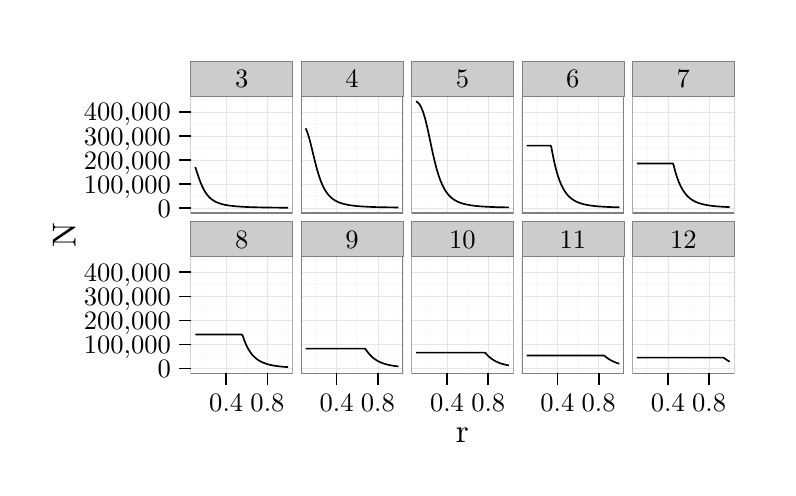
\begin{tikzpicture}[x=1pt,y=1pt]
\definecolor[named]{fillColor}{rgb}{1.00,1.00,1.00}
\path[use as bounding box,fill=fillColor,fill opacity=0.00] (0,0) rectangle (267.40,158.99);
\begin{scope}
\path[clip] (  0.00,  0.00) rectangle (267.40,158.99);
\definecolor[named]{drawColor}{rgb}{1.00,1.00,1.00}
\definecolor[named]{fillColor}{rgb}{1.00,1.00,1.00}

\path[draw=drawColor,line width= 0.6pt,line join=round,line cap=round,fill=fillColor] ( -0.00,  0.00) rectangle (267.40,158.99);
\end{scope}
\begin{scope}
\path[clip] ( 58.88, 92.00) rectangle ( 95.77,134.31);
\definecolor[named]{fillColor}{rgb}{1.00,1.00,1.00}

\path[fill=fillColor] ( 58.88, 92.00) rectangle ( 95.77,134.31);
\definecolor[named]{drawColor}{rgb}{0.98,0.98,0.98}

\path[draw=drawColor,line width= 0.6pt,line join=round] ( 58.88, 98.11) --
	( 95.77, 98.11);

\path[draw=drawColor,line width= 0.6pt,line join=round] ( 58.88,106.81) --
	( 95.77,106.81);

\path[draw=drawColor,line width= 0.6pt,line join=round] ( 58.88,115.52) --
	( 95.77,115.52);

\path[draw=drawColor,line width= 0.6pt,line join=round] ( 58.88,124.22) --
	( 95.77,124.22);

\path[draw=drawColor,line width= 0.6pt,line join=round] ( 58.88,132.92) --
	( 95.77,132.92);

\path[draw=drawColor,line width= 0.6pt,line join=round] ( 64.28, 92.00) --
	( 64.28,134.31);

\path[draw=drawColor,line width= 0.6pt,line join=round] ( 79.19, 92.00) --
	( 79.19,134.31);

\path[draw=drawColor,line width= 0.6pt,line join=round] ( 94.09, 92.00) --
	( 94.09,134.31);
\definecolor[named]{drawColor}{rgb}{0.90,0.90,0.90}

\path[draw=drawColor,line width= 0.2pt,line join=round] ( 58.88, 93.76) --
	( 95.77, 93.76);

\path[draw=drawColor,line width= 0.2pt,line join=round] ( 58.88,102.46) --
	( 95.77,102.46);

\path[draw=drawColor,line width= 0.2pt,line join=round] ( 58.88,111.16) --
	( 95.77,111.16);

\path[draw=drawColor,line width= 0.2pt,line join=round] ( 58.88,119.87) --
	( 95.77,119.87);

\path[draw=drawColor,line width= 0.2pt,line join=round] ( 58.88,128.57) --
	( 95.77,128.57);

\path[draw=drawColor,line width= 0.2pt,line join=round] ( 71.74, 92.00) --
	( 71.74,134.31);

\path[draw=drawColor,line width= 0.2pt,line join=round] ( 86.64, 92.00) --
	( 86.64,134.31);
\definecolor[named]{drawColor}{rgb}{0.00,0.00,0.00}

\path[draw=drawColor,line width= 0.6pt,line join=round] ( 60.56,108.63) --
	( 60.93,107.49) --
	( 61.30,106.35) --
	( 61.68,105.23) --
	( 62.05,104.17) --
	( 62.42,103.18) --
	( 62.79,102.27) --
	( 63.17,101.43) --
	( 63.54,100.68) --
	( 63.91,100.01) --
	( 64.28, 99.40) --
	( 64.66, 98.86) --
	( 65.03, 98.39) --
	( 65.40, 97.96) --
	( 65.77, 97.58) --
	( 66.15, 97.25) --
	( 66.52, 96.95) --
	( 66.89, 96.68) --
	( 67.27, 96.44) --
	( 67.64, 96.23) --
	( 68.01, 96.03) --
	( 68.38, 95.86) --
	( 68.76, 95.71) --
	( 69.13, 95.57) --
	( 69.50, 95.44) --
	( 69.87, 95.33) --
	( 70.25, 95.22) --
	( 70.62, 95.13) --
	( 70.99, 95.04) --
	( 71.36, 94.96) --
	( 71.74, 94.89) --
	( 72.11, 94.83) --
	( 72.48, 94.76) --
	( 72.85, 94.71) --
	( 73.23, 94.66) --
	( 73.60, 94.61) --
	( 73.97, 94.57) --
	( 74.34, 94.53) --
	( 74.72, 94.49) --
	( 75.09, 94.45) --
	( 75.46, 94.42) --
	( 75.83, 94.39) --
	( 76.21, 94.36) --
	( 76.58, 94.34) --
	( 76.95, 94.31) --
	( 77.32, 94.29) --
	( 77.70, 94.27) --
	( 78.07, 94.25) --
	( 78.44, 94.23) --
	( 78.82, 94.21) --
	( 79.19, 94.19) --
	( 79.56, 94.18) --
	( 79.93, 94.16) --
	( 80.31, 94.15) --
	( 80.68, 94.14) --
	( 81.05, 94.12) --
	( 81.42, 94.11) --
	( 81.80, 94.10) --
	( 82.17, 94.09) --
	( 82.54, 94.08) --
	( 82.91, 94.07) --
	( 83.29, 94.06) --
	( 83.66, 94.05) --
	( 84.03, 94.04) --
	( 84.40, 94.04) --
	( 84.78, 94.03) --
	( 85.15, 94.02) --
	( 85.52, 94.01) --
	( 85.89, 94.01) --
	( 86.27, 94.00) --
	( 86.64, 94.00) --
	( 87.01, 93.99) --
	( 87.38, 93.99) --
	( 87.76, 93.98) --
	( 88.13, 93.98) --
	( 88.50, 93.97) --
	( 88.87, 93.97) --
	( 89.25, 93.96) --
	( 89.62, 93.96) --
	( 89.99, 93.95) --
	( 90.37, 93.95) --
	( 90.74, 93.95) --
	( 91.11, 93.94) --
	( 91.48, 93.94) --
	( 91.86, 93.94) --
	( 92.23, 93.93) --
	( 92.60, 93.93) --
	( 92.97, 93.93) --
	( 93.35, 93.93) --
	( 93.72, 93.92) --
	( 94.09, 93.92);
\definecolor[named]{drawColor}{rgb}{0.50,0.50,0.50}

\path[draw=drawColor,line width= 0.6pt,line join=round,line cap=round] ( 58.88, 92.00) rectangle ( 95.77,134.31);
\end{scope}
\begin{scope}
\path[clip] ( 98.78, 92.00) rectangle (135.66,134.31);
\definecolor[named]{fillColor}{rgb}{1.00,1.00,1.00}

\path[fill=fillColor] ( 98.78, 92.00) rectangle (135.66,134.31);
\definecolor[named]{drawColor}{rgb}{0.98,0.98,0.98}

\path[draw=drawColor,line width= 0.6pt,line join=round] ( 98.78, 98.11) --
	(135.66, 98.11);

\path[draw=drawColor,line width= 0.6pt,line join=round] ( 98.78,106.81) --
	(135.66,106.81);

\path[draw=drawColor,line width= 0.6pt,line join=round] ( 98.78,115.52) --
	(135.66,115.52);

\path[draw=drawColor,line width= 0.6pt,line join=round] ( 98.78,124.22) --
	(135.66,124.22);

\path[draw=drawColor,line width= 0.6pt,line join=round] ( 98.78,132.92) --
	(135.66,132.92);

\path[draw=drawColor,line width= 0.6pt,line join=round] (104.18, 92.00) --
	(104.18,134.31);

\path[draw=drawColor,line width= 0.6pt,line join=round] (119.08, 92.00) --
	(119.08,134.31);

\path[draw=drawColor,line width= 0.6pt,line join=round] (133.99, 92.00) --
	(133.99,134.31);
\definecolor[named]{drawColor}{rgb}{0.90,0.90,0.90}

\path[draw=drawColor,line width= 0.2pt,line join=round] ( 98.78, 93.76) --
	(135.66, 93.76);

\path[draw=drawColor,line width= 0.2pt,line join=round] ( 98.78,102.46) --
	(135.66,102.46);

\path[draw=drawColor,line width= 0.2pt,line join=round] ( 98.78,111.16) --
	(135.66,111.16);

\path[draw=drawColor,line width= 0.2pt,line join=round] ( 98.78,119.87) --
	(135.66,119.87);

\path[draw=drawColor,line width= 0.2pt,line join=round] ( 98.78,128.57) --
	(135.66,128.57);

\path[draw=drawColor,line width= 0.2pt,line join=round] (111.63, 92.00) --
	(111.63,134.31);

\path[draw=drawColor,line width= 0.2pt,line join=round] (126.54, 92.00) --
	(126.54,134.31);
\definecolor[named]{drawColor}{rgb}{0.00,0.00,0.00}

\path[draw=drawColor,line width= 0.6pt,line join=round] (100.46,122.63) --
	(100.83,121.78) --
	(101.20,120.76) --
	(101.57,119.58) --
	(101.95,118.25) --
	(102.32,116.81) --
	(102.69,115.29) --
	(103.06,113.74) --
	(103.44,112.19) --
	(103.81,110.67) --
	(104.18,109.21) --
	(104.55,107.83) --
	(104.93,106.54) --
	(105.30,105.34) --
	(105.67,104.25) --
	(106.04,103.26) --
	(106.42,102.36) --
	(106.79,101.55) --
	(107.16,100.82) --
	(107.53,100.17) --
	(107.91, 99.59) --
	(108.28, 99.07) --
	(108.65, 98.60) --
	(109.02, 98.19) --
	(109.40, 97.81) --
	(109.77, 97.48) --
	(110.14, 97.18) --
	(110.51, 96.91) --
	(110.89, 96.67) --
	(111.26, 96.45) --
	(111.63, 96.25) --
	(112.01, 96.07) --
	(112.38, 95.91) --
	(112.75, 95.76) --
	(113.12, 95.63) --
	(113.50, 95.51) --
	(113.87, 95.39) --
	(114.24, 95.29) --
	(114.61, 95.20) --
	(114.99, 95.12) --
	(115.36, 95.04) --
	(115.73, 94.97) --
	(116.10, 94.90) --
	(116.48, 94.84) --
	(116.85, 94.78) --
	(117.22, 94.73) --
	(117.59, 94.68) --
	(117.97, 94.64) --
	(118.34, 94.60) --
	(118.71, 94.56) --
	(119.08, 94.52) --
	(119.46, 94.49) --
	(119.83, 94.46) --
	(120.20, 94.43) --
	(120.57, 94.40) --
	(120.95, 94.38) --
	(121.32, 94.35) --
	(121.69, 94.33) --
	(122.06, 94.31) --
	(122.44, 94.29) --
	(122.81, 94.27) --
	(123.18, 94.25) --
	(123.56, 94.24) --
	(123.93, 94.22) --
	(124.30, 94.21) --
	(124.67, 94.19) --
	(125.05, 94.18) --
	(125.42, 94.17) --
	(125.79, 94.16) --
	(126.16, 94.15) --
	(126.54, 94.14) --
	(126.91, 94.13) --
	(127.28, 94.12) --
	(127.65, 94.11) --
	(128.03, 94.10) --
	(128.40, 94.09) --
	(128.77, 94.09) --
	(129.14, 94.08) --
	(129.52, 94.07) --
	(129.89, 94.07) --
	(130.26, 94.06) --
	(130.63, 94.06) --
	(131.01, 94.05) --
	(131.38, 94.05) --
	(131.75, 94.04) --
	(132.12, 94.04) --
	(132.50, 94.03) --
	(132.87, 94.03) --
	(133.24, 94.03) --
	(133.61, 94.02) --
	(133.99, 94.02);
\definecolor[named]{drawColor}{rgb}{0.50,0.50,0.50}

\path[draw=drawColor,line width= 0.6pt,line join=round,line cap=round] ( 98.78, 92.00) rectangle (135.66,134.31);
\end{scope}
\begin{scope}
\path[clip] (138.68, 92.00) rectangle (175.56,134.31);
\definecolor[named]{fillColor}{rgb}{1.00,1.00,1.00}

\path[fill=fillColor] (138.68, 92.00) rectangle (175.56,134.31);
\definecolor[named]{drawColor}{rgb}{0.98,0.98,0.98}

\path[draw=drawColor,line width= 0.6pt,line join=round] (138.68, 98.11) --
	(175.56, 98.11);

\path[draw=drawColor,line width= 0.6pt,line join=round] (138.68,106.81) --
	(175.56,106.81);

\path[draw=drawColor,line width= 0.6pt,line join=round] (138.68,115.52) --
	(175.56,115.52);

\path[draw=drawColor,line width= 0.6pt,line join=round] (138.68,124.22) --
	(175.56,124.22);

\path[draw=drawColor,line width= 0.6pt,line join=round] (138.68,132.92) --
	(175.56,132.92);

\path[draw=drawColor,line width= 0.6pt,line join=round] (144.08, 92.00) --
	(144.08,134.31);

\path[draw=drawColor,line width= 0.6pt,line join=round] (158.98, 92.00) --
	(158.98,134.31);

\path[draw=drawColor,line width= 0.6pt,line join=round] (173.88, 92.00) --
	(173.88,134.31);
\definecolor[named]{drawColor}{rgb}{0.90,0.90,0.90}

\path[draw=drawColor,line width= 0.2pt,line join=round] (138.68, 93.76) --
	(175.56, 93.76);

\path[draw=drawColor,line width= 0.2pt,line join=round] (138.68,102.46) --
	(175.56,102.46);

\path[draw=drawColor,line width= 0.2pt,line join=round] (138.68,111.16) --
	(175.56,111.16);

\path[draw=drawColor,line width= 0.2pt,line join=round] (138.68,119.87) --
	(175.56,119.87);

\path[draw=drawColor,line width= 0.2pt,line join=round] (138.68,128.57) --
	(175.56,128.57);

\path[draw=drawColor,line width= 0.2pt,line join=round] (151.53, 92.00) --
	(151.53,134.31);

\path[draw=drawColor,line width= 0.2pt,line join=round] (166.43, 92.00) --
	(166.43,134.31);
\definecolor[named]{drawColor}{rgb}{0.00,0.00,0.00}

\path[draw=drawColor,line width= 0.6pt,line join=round] (140.35,132.39) --
	(140.72,132.16) --
	(141.10,131.84) --
	(141.47,131.41) --
	(141.84,130.85) --
	(142.21,130.15) --
	(142.59,129.29) --
	(142.96,128.27) --
	(143.33,127.08) --
	(143.71,125.74) --
	(144.08,124.26) --
	(144.45,122.66) --
	(144.82,120.97) --
	(145.20,119.23) --
	(145.57,117.46) --
	(145.94,115.70) --
	(146.31,113.98) --
	(146.69,112.33) --
	(147.06,110.75) --
	(147.43,109.27) --
	(147.80,107.89) --
	(148.18,106.61) --
	(148.55,105.44) --
	(148.92,104.37) --
	(149.29,103.39) --
	(149.67,102.51) --
	(150.04,101.72) --
	(150.41,101.00) --
	(150.78,100.35) --
	(151.16, 99.77) --
	(151.53, 99.25) --
	(151.90, 98.78) --
	(152.27, 98.36) --
	(152.65, 97.98) --
	(153.02, 97.64) --
	(153.39, 97.33) --
	(153.76, 97.05) --
	(154.14, 96.80) --
	(154.51, 96.57) --
	(154.88, 96.36) --
	(155.26, 96.17) --
	(155.63, 96.00) --
	(156.00, 95.85) --
	(156.37, 95.71) --
	(156.75, 95.58) --
	(157.12, 95.46) --
	(157.49, 95.35) --
	(157.86, 95.26) --
	(158.24, 95.17) --
	(158.61, 95.08) --
	(158.98, 95.01) --
	(159.35, 94.94) --
	(159.73, 94.87) --
	(160.10, 94.81) --
	(160.47, 94.75) --
	(160.84, 94.70) --
	(161.22, 94.66) --
	(161.59, 94.61) --
	(161.96, 94.57) --
	(162.33, 94.53) --
	(162.71, 94.50) --
	(163.08, 94.46) --
	(163.45, 94.43) --
	(163.82, 94.40) --
	(164.20, 94.38) --
	(164.57, 94.35) --
	(164.94, 94.33) --
	(165.31, 94.31) --
	(165.69, 94.29) --
	(166.06, 94.27) --
	(166.43, 94.25) --
	(166.81, 94.23) --
	(167.18, 94.21) --
	(167.55, 94.20) --
	(167.92, 94.18) --
	(168.30, 94.17) --
	(168.67, 94.16) --
	(169.04, 94.15) --
	(169.41, 94.14) --
	(169.79, 94.12) --
	(170.16, 94.11) --
	(170.53, 94.11) --
	(170.90, 94.10) --
	(171.28, 94.09) --
	(171.65, 94.08) --
	(172.02, 94.07) --
	(172.39, 94.07) --
	(172.77, 94.06) --
	(173.14, 94.05) --
	(173.51, 94.05) --
	(173.88, 94.04);
\definecolor[named]{drawColor}{rgb}{0.50,0.50,0.50}

\path[draw=drawColor,line width= 0.6pt,line join=round,line cap=round] (138.68, 92.00) rectangle (175.56,134.31);
\end{scope}
\begin{scope}
\path[clip] (178.57, 92.00) rectangle (215.46,134.31);
\definecolor[named]{fillColor}{rgb}{1.00,1.00,1.00}

\path[fill=fillColor] (178.57, 92.00) rectangle (215.46,134.31);
\definecolor[named]{drawColor}{rgb}{0.98,0.98,0.98}

\path[draw=drawColor,line width= 0.6pt,line join=round] (178.57, 98.11) --
	(215.46, 98.11);

\path[draw=drawColor,line width= 0.6pt,line join=round] (178.57,106.81) --
	(215.46,106.81);

\path[draw=drawColor,line width= 0.6pt,line join=round] (178.57,115.52) --
	(215.46,115.52);

\path[draw=drawColor,line width= 0.6pt,line join=round] (178.57,124.22) --
	(215.46,124.22);

\path[draw=drawColor,line width= 0.6pt,line join=round] (178.57,132.92) --
	(215.46,132.92);

\path[draw=drawColor,line width= 0.6pt,line join=round] (183.97, 92.00) --
	(183.97,134.31);

\path[draw=drawColor,line width= 0.6pt,line join=round] (198.88, 92.00) --
	(198.88,134.31);

\path[draw=drawColor,line width= 0.6pt,line join=round] (213.78, 92.00) --
	(213.78,134.31);
\definecolor[named]{drawColor}{rgb}{0.90,0.90,0.90}

\path[draw=drawColor,line width= 0.2pt,line join=round] (178.57, 93.76) --
	(215.46, 93.76);

\path[draw=drawColor,line width= 0.2pt,line join=round] (178.57,102.46) --
	(215.46,102.46);

\path[draw=drawColor,line width= 0.2pt,line join=round] (178.57,111.16) --
	(215.46,111.16);

\path[draw=drawColor,line width= 0.2pt,line join=round] (178.57,119.87) --
	(215.46,119.87);

\path[draw=drawColor,line width= 0.2pt,line join=round] (178.57,128.57) --
	(215.46,128.57);

\path[draw=drawColor,line width= 0.2pt,line join=round] (191.43, 92.00) --
	(191.43,134.31);

\path[draw=drawColor,line width= 0.2pt,line join=round] (206.33, 92.00) --
	(206.33,134.31);
\definecolor[named]{drawColor}{rgb}{0.00,0.00,0.00}

\path[draw=drawColor,line width= 0.6pt,line join=round] (180.25,116.38) --
	(180.62,116.38) --
	(180.99,116.38) --
	(181.37,116.38) --
	(181.74,116.38) --
	(182.11,116.38) --
	(182.48,116.38) --
	(182.86,116.38) --
	(183.23,116.38) --
	(183.60,116.38) --
	(183.97,116.38) --
	(184.35,116.38) --
	(184.72,116.38) --
	(185.09,116.38) --
	(185.46,116.38) --
	(185.84,116.38) --
	(186.21,116.38) --
	(186.58,116.38) --
	(186.95,116.38) --
	(187.33,116.38) --
	(187.70,116.38) --
	(188.07,116.38) --
	(188.45,116.38) --
	(188.82,116.38) --
	(189.19,116.01) --
	(189.56,113.97) --
	(189.94,112.08) --
	(190.31,110.34) --
	(190.68,108.76) --
	(191.05,107.32) --
	(191.43,106.02) --
	(191.80,104.85) --
	(192.17,103.79) --
	(192.54,102.85) --
	(192.92,102.00) --
	(193.29,101.23) --
	(193.66,100.55) --
	(194.03, 99.94) --
	(194.41, 99.39) --
	(194.78, 98.90) --
	(195.15, 98.46) --
	(195.52, 98.06) --
	(195.90, 97.71) --
	(196.27, 97.39) --
	(196.64, 97.10) --
	(197.01, 96.84) --
	(197.39, 96.60) --
	(197.76, 96.38) --
	(198.13, 96.19) --
	(198.50, 96.02) --
	(198.88, 95.86) --
	(199.25, 95.71) --
	(199.62, 95.58) --
	(200.00, 95.46) --
	(200.37, 95.35) --
	(200.74, 95.24) --
	(201.11, 95.15) --
	(201.49, 95.07) --
	(201.86, 94.99) --
	(202.23, 94.91) --
	(202.60, 94.85) --
	(202.98, 94.79) --
	(203.35, 94.73) --
	(203.72, 94.68) --
	(204.09, 94.63) --
	(204.47, 94.58) --
	(204.84, 94.54) --
	(205.21, 94.50) --
	(205.58, 94.47) --
	(205.96, 94.44) --
	(206.33, 94.40) --
	(206.70, 94.38) --
	(207.07, 94.35) --
	(207.45, 94.32) --
	(207.82, 94.30) --
	(208.19, 94.28) --
	(208.56, 94.26) --
	(208.94, 94.24) --
	(209.31, 94.22) --
	(209.68, 94.20) --
	(210.05, 94.19) --
	(210.43, 94.17) --
	(210.80, 94.16) --
	(211.17, 94.14) --
	(211.55, 94.13) --
	(211.92, 94.12) --
	(212.29, 94.11) --
	(212.66, 94.10) --
	(213.04, 94.09) --
	(213.41, 94.08) --
	(213.78, 94.07);
\definecolor[named]{drawColor}{rgb}{0.50,0.50,0.50}

\path[draw=drawColor,line width= 0.6pt,line join=round,line cap=round] (178.57, 92.00) rectangle (215.46,134.31);
\end{scope}
\begin{scope}
\path[clip] (218.47, 92.00) rectangle (255.35,134.31);
\definecolor[named]{fillColor}{rgb}{1.00,1.00,1.00}

\path[fill=fillColor] (218.47, 92.00) rectangle (255.35,134.31);
\definecolor[named]{drawColor}{rgb}{0.98,0.98,0.98}

\path[draw=drawColor,line width= 0.6pt,line join=round] (218.47, 98.11) --
	(255.35, 98.11);

\path[draw=drawColor,line width= 0.6pt,line join=round] (218.47,106.81) --
	(255.35,106.81);

\path[draw=drawColor,line width= 0.6pt,line join=round] (218.47,115.52) --
	(255.35,115.52);

\path[draw=drawColor,line width= 0.6pt,line join=round] (218.47,124.22) --
	(255.35,124.22);

\path[draw=drawColor,line width= 0.6pt,line join=round] (218.47,132.92) --
	(255.35,132.92);

\path[draw=drawColor,line width= 0.6pt,line join=round] (223.87, 92.00) --
	(223.87,134.31);

\path[draw=drawColor,line width= 0.6pt,line join=round] (238.77, 92.00) --
	(238.77,134.31);

\path[draw=drawColor,line width= 0.6pt,line join=round] (253.68, 92.00) --
	(253.68,134.31);
\definecolor[named]{drawColor}{rgb}{0.90,0.90,0.90}

\path[draw=drawColor,line width= 0.2pt,line join=round] (218.47, 93.76) --
	(255.35, 93.76);

\path[draw=drawColor,line width= 0.2pt,line join=round] (218.47,102.46) --
	(255.35,102.46);

\path[draw=drawColor,line width= 0.2pt,line join=round] (218.47,111.16) --
	(255.35,111.16);

\path[draw=drawColor,line width= 0.2pt,line join=round] (218.47,119.87) --
	(255.35,119.87);

\path[draw=drawColor,line width= 0.2pt,line join=round] (218.47,128.57) --
	(255.35,128.57);

\path[draw=drawColor,line width= 0.2pt,line join=round] (231.32, 92.00) --
	(231.32,134.31);

\path[draw=drawColor,line width= 0.2pt,line join=round] (246.23, 92.00) --
	(246.23,134.31);
\definecolor[named]{drawColor}{rgb}{0.00,0.00,0.00}

\path[draw=drawColor,line width= 0.6pt,line join=round] (220.15,109.90) --
	(220.52,109.90) --
	(220.89,109.90) --
	(221.26,109.90) --
	(221.64,109.90) --
	(222.01,109.90) --
	(222.38,109.90) --
	(222.75,109.90) --
	(223.13,109.90) --
	(223.50,109.90) --
	(223.87,109.90) --
	(224.24,109.90) --
	(224.62,109.90) --
	(224.99,109.90) --
	(225.36,109.90) --
	(225.73,109.90) --
	(226.11,109.90) --
	(226.48,109.90) --
	(226.85,109.90) --
	(227.22,109.90) --
	(227.60,109.90) --
	(227.97,109.90) --
	(228.34,109.90) --
	(228.71,109.90) --
	(229.09,109.90) --
	(229.46,109.90) --
	(229.83,109.90) --
	(230.20,109.90) --
	(230.58,109.90) --
	(230.95,109.90) --
	(231.32,109.90) --
	(231.70,109.90) --
	(232.07,109.90) --
	(232.44,109.90) --
	(232.81,109.90) --
	(233.19,109.90) --
	(233.56,108.72) --
	(233.93,107.31) --
	(234.30,106.03) --
	(234.68,104.88) --
	(235.05,103.84) --
	(235.42,102.91) --
	(235.79,102.07) --
	(236.17,101.31) --
	(236.54,100.64) --
	(236.91,100.03) --
	(237.28, 99.48) --
	(237.66, 98.99) --
	(238.03, 98.54) --
	(238.40, 98.14) --
	(238.77, 97.78) --
	(239.15, 97.46) --
	(239.52, 97.17) --
	(239.89, 96.90) --
	(240.26, 96.66) --
	(240.64, 96.44) --
	(241.01, 96.24) --
	(241.38, 96.06) --
	(241.75, 95.90) --
	(242.13, 95.75) --
	(242.50, 95.61) --
	(242.87, 95.49) --
	(243.25, 95.38) --
	(243.62, 95.27) --
	(243.99, 95.18) --
	(244.36, 95.09) --
	(244.74, 95.01) --
	(245.11, 94.93) --
	(245.48, 94.86) --
	(245.85, 94.80) --
	(246.23, 94.74) --
	(246.60, 94.69) --
	(246.97, 94.64) --
	(247.34, 94.59) --
	(247.72, 94.55) --
	(248.09, 94.51) --
	(248.46, 94.47) --
	(248.83, 94.44) --
	(249.21, 94.41) --
	(249.58, 94.38) --
	(249.95, 94.35) --
	(250.32, 94.32) --
	(250.70, 94.30) --
	(251.07, 94.28) --
	(251.44, 94.26) --
	(251.81, 94.24) --
	(252.19, 94.22) --
	(252.56, 94.20) --
	(252.93, 94.18) --
	(253.30, 94.17) --
	(253.68, 94.15);
\definecolor[named]{drawColor}{rgb}{0.50,0.50,0.50}

\path[draw=drawColor,line width= 0.6pt,line join=round,line cap=round] (218.47, 92.00) rectangle (255.35,134.31);
\end{scope}
\begin{scope}
\path[clip] ( 58.88, 34.03) rectangle ( 95.77, 76.35);
\definecolor[named]{fillColor}{rgb}{1.00,1.00,1.00}

\path[fill=fillColor] ( 58.88, 34.03) rectangle ( 95.77, 76.35);
\definecolor[named]{drawColor}{rgb}{0.98,0.98,0.98}

\path[draw=drawColor,line width= 0.6pt,line join=round] ( 58.88, 40.15) --
	( 95.77, 40.15);

\path[draw=drawColor,line width= 0.6pt,line join=round] ( 58.88, 48.85) --
	( 95.77, 48.85);

\path[draw=drawColor,line width= 0.6pt,line join=round] ( 58.88, 57.55) --
	( 95.77, 57.55);

\path[draw=drawColor,line width= 0.6pt,line join=round] ( 58.88, 66.26) --
	( 95.77, 66.26);

\path[draw=drawColor,line width= 0.6pt,line join=round] ( 58.88, 74.96) --
	( 95.77, 74.96);

\path[draw=drawColor,line width= 0.6pt,line join=round] ( 64.28, 34.03) --
	( 64.28, 76.35);

\path[draw=drawColor,line width= 0.6pt,line join=round] ( 79.19, 34.03) --
	( 79.19, 76.35);

\path[draw=drawColor,line width= 0.6pt,line join=round] ( 94.09, 34.03) --
	( 94.09, 76.35);
\definecolor[named]{drawColor}{rgb}{0.90,0.90,0.90}

\path[draw=drawColor,line width= 0.2pt,line join=round] ( 58.88, 35.79) --
	( 95.77, 35.79);

\path[draw=drawColor,line width= 0.2pt,line join=round] ( 58.88, 44.50) --
	( 95.77, 44.50);

\path[draw=drawColor,line width= 0.2pt,line join=round] ( 58.88, 53.20) --
	( 95.77, 53.20);

\path[draw=drawColor,line width= 0.2pt,line join=round] ( 58.88, 61.90) --
	( 95.77, 61.90);

\path[draw=drawColor,line width= 0.2pt,line join=round] ( 58.88, 70.61) --
	( 95.77, 70.61);

\path[draw=drawColor,line width= 0.2pt,line join=round] ( 71.74, 34.03) --
	( 71.74, 76.35);

\path[draw=drawColor,line width= 0.2pt,line join=round] ( 86.64, 34.03) --
	( 86.64, 76.35);
\definecolor[named]{drawColor}{rgb}{0.00,0.00,0.00}

\path[draw=drawColor,line width= 0.6pt,line join=round] ( 60.56, 48.13) --
	( 60.93, 48.13) --
	( 61.30, 48.13) --
	( 61.68, 48.13) --
	( 62.05, 48.13) --
	( 62.42, 48.13) --
	( 62.79, 48.13) --
	( 63.17, 48.13) --
	( 63.54, 48.13) --
	( 63.91, 48.13) --
	( 64.28, 48.13) --
	( 64.66, 48.13) --
	( 65.03, 48.13) --
	( 65.40, 48.13) --
	( 65.77, 48.13) --
	( 66.15, 48.13) --
	( 66.52, 48.13) --
	( 66.89, 48.13) --
	( 67.27, 48.13) --
	( 67.64, 48.13) --
	( 68.01, 48.13) --
	( 68.38, 48.13) --
	( 68.76, 48.13) --
	( 69.13, 48.13) --
	( 69.50, 48.13) --
	( 69.87, 48.13) --
	( 70.25, 48.13) --
	( 70.62, 48.13) --
	( 70.99, 48.13) --
	( 71.36, 48.13) --
	( 71.74, 48.13) --
	( 72.11, 48.13) --
	( 72.48, 48.13) --
	( 72.85, 48.13) --
	( 73.23, 48.13) --
	( 73.60, 48.13) --
	( 73.97, 48.13) --
	( 74.34, 48.13) --
	( 74.72, 48.13) --
	( 75.09, 48.13) --
	( 75.46, 48.13) --
	( 75.83, 48.13) --
	( 76.21, 48.13) --
	( 76.58, 48.13) --
	( 76.95, 48.13) --
	( 77.32, 48.13) --
	( 77.70, 47.69) --
	( 78.07, 46.59) --
	( 78.44, 45.60) --
	( 78.82, 44.70) --
	( 79.19, 43.90) --
	( 79.56, 43.17) --
	( 79.93, 42.52) --
	( 80.31, 41.94) --
	( 80.68, 41.41) --
	( 81.05, 40.93) --
	( 81.42, 40.50) --
	( 81.80, 40.12) --
	( 82.17, 39.76) --
	( 82.54, 39.45) --
	( 82.91, 39.16) --
	( 83.29, 38.90) --
	( 83.66, 38.67) --
	( 84.03, 38.45) --
	( 84.40, 38.26) --
	( 84.78, 38.08) --
	( 85.15, 37.92) --
	( 85.52, 37.77) --
	( 85.89, 37.64) --
	( 86.27, 37.51) --
	( 86.64, 37.40) --
	( 87.01, 37.30) --
	( 87.38, 37.20) --
	( 87.76, 37.12) --
	( 88.13, 37.04) --
	( 88.50, 36.96) --
	( 88.87, 36.89) --
	( 89.25, 36.83) --
	( 89.62, 36.77) --
	( 89.99, 36.72) --
	( 90.37, 36.67) --
	( 90.74, 36.62) --
	( 91.11, 36.58) --
	( 91.48, 36.54) --
	( 91.86, 36.50) --
	( 92.23, 36.47) --
	( 92.60, 36.44) --
	( 92.97, 36.41) --
	( 93.35, 36.38) --
	( 93.72, 36.35) --
	( 94.09, 36.33);
\definecolor[named]{drawColor}{rgb}{0.50,0.50,0.50}

\path[draw=drawColor,line width= 0.6pt,line join=round,line cap=round] ( 58.88, 34.03) rectangle ( 95.77, 76.35);
\end{scope}
\begin{scope}
\path[clip] ( 98.78, 34.03) rectangle (135.66, 76.35);
\definecolor[named]{fillColor}{rgb}{1.00,1.00,1.00}

\path[fill=fillColor] ( 98.78, 34.03) rectangle (135.66, 76.35);
\definecolor[named]{drawColor}{rgb}{0.98,0.98,0.98}

\path[draw=drawColor,line width= 0.6pt,line join=round] ( 98.78, 40.15) --
	(135.66, 40.15);

\path[draw=drawColor,line width= 0.6pt,line join=round] ( 98.78, 48.85) --
	(135.66, 48.85);

\path[draw=drawColor,line width= 0.6pt,line join=round] ( 98.78, 57.55) --
	(135.66, 57.55);

\path[draw=drawColor,line width= 0.6pt,line join=round] ( 98.78, 66.26) --
	(135.66, 66.26);

\path[draw=drawColor,line width= 0.6pt,line join=round] ( 98.78, 74.96) --
	(135.66, 74.96);

\path[draw=drawColor,line width= 0.6pt,line join=round] (104.18, 34.03) --
	(104.18, 76.35);

\path[draw=drawColor,line width= 0.6pt,line join=round] (119.08, 34.03) --
	(119.08, 76.35);

\path[draw=drawColor,line width= 0.6pt,line join=round] (133.99, 34.03) --
	(133.99, 76.35);
\definecolor[named]{drawColor}{rgb}{0.90,0.90,0.90}

\path[draw=drawColor,line width= 0.2pt,line join=round] ( 98.78, 35.79) --
	(135.66, 35.79);

\path[draw=drawColor,line width= 0.2pt,line join=round] ( 98.78, 44.50) --
	(135.66, 44.50);

\path[draw=drawColor,line width= 0.2pt,line join=round] ( 98.78, 53.20) --
	(135.66, 53.20);

\path[draw=drawColor,line width= 0.2pt,line join=round] ( 98.78, 61.90) --
	(135.66, 61.90);

\path[draw=drawColor,line width= 0.2pt,line join=round] ( 98.78, 70.61) --
	(135.66, 70.61);

\path[draw=drawColor,line width= 0.2pt,line join=round] (111.63, 34.03) --
	(111.63, 76.35);

\path[draw=drawColor,line width= 0.2pt,line join=round] (126.54, 34.03) --
	(126.54, 76.35);
\definecolor[named]{drawColor}{rgb}{0.00,0.00,0.00}

\path[draw=drawColor,line width= 0.6pt,line join=round] (100.46, 43.01) --
	(100.83, 43.01) --
	(101.20, 43.01) --
	(101.57, 43.01) --
	(101.95, 43.01) --
	(102.32, 43.01) --
	(102.69, 43.01) --
	(103.06, 43.01) --
	(103.44, 43.01) --
	(103.81, 43.01) --
	(104.18, 43.01) --
	(104.55, 43.01) --
	(104.93, 43.01) --
	(105.30, 43.01) --
	(105.67, 43.01) --
	(106.04, 43.01) --
	(106.42, 43.01) --
	(106.79, 43.01) --
	(107.16, 43.01) --
	(107.53, 43.01) --
	(107.91, 43.01) --
	(108.28, 43.01) --
	(108.65, 43.01) --
	(109.02, 43.01) --
	(109.40, 43.01) --
	(109.77, 43.01) --
	(110.14, 43.01) --
	(110.51, 43.01) --
	(110.89, 43.01) --
	(111.26, 43.01) --
	(111.63, 43.01) --
	(112.01, 43.01) --
	(112.38, 43.01) --
	(112.75, 43.01) --
	(113.12, 43.01) --
	(113.50, 43.01) --
	(113.87, 43.01) --
	(114.24, 43.01) --
	(114.61, 43.01) --
	(114.99, 43.01) --
	(115.36, 43.01) --
	(115.73, 43.01) --
	(116.10, 43.01) --
	(116.48, 43.01) --
	(116.85, 43.01) --
	(117.22, 43.01) --
	(117.59, 43.01) --
	(117.97, 43.01) --
	(118.34, 43.01) --
	(118.71, 43.01) --
	(119.08, 43.01) --
	(119.46, 43.01) --
	(119.83, 43.01) --
	(120.20, 43.01) --
	(120.57, 43.01) --
	(120.95, 43.01) --
	(121.32, 43.01) --
	(121.69, 43.01) --
	(122.06, 42.92) --
	(122.44, 42.35) --
	(122.81, 41.83) --
	(123.18, 41.35) --
	(123.56, 40.91) --
	(123.93, 40.52) --
	(124.30, 40.15) --
	(124.67, 39.82) --
	(125.05, 39.51) --
	(125.42, 39.23) --
	(125.79, 38.98) --
	(126.16, 38.75) --
	(126.54, 38.53) --
	(126.91, 38.34) --
	(127.28, 38.16) --
	(127.65, 38.00) --
	(128.03, 37.85) --
	(128.40, 37.71) --
	(128.77, 37.59) --
	(129.14, 37.47) --
	(129.52, 37.36) --
	(129.89, 37.27) --
	(130.26, 37.18) --
	(130.63, 37.09) --
	(131.01, 37.02) --
	(131.38, 36.94) --
	(131.75, 36.88) --
	(132.12, 36.82) --
	(132.50, 36.76) --
	(132.87, 36.71) --
	(133.24, 36.66) --
	(133.61, 36.62) --
	(133.99, 36.58);
\definecolor[named]{drawColor}{rgb}{0.50,0.50,0.50}

\path[draw=drawColor,line width= 0.6pt,line join=round,line cap=round] ( 98.78, 34.03) rectangle (135.66, 76.35);
\end{scope}
\begin{scope}
\path[clip] (138.68, 34.03) rectangle (175.56, 76.35);
\definecolor[named]{fillColor}{rgb}{1.00,1.00,1.00}

\path[fill=fillColor] (138.68, 34.03) rectangle (175.56, 76.35);
\definecolor[named]{drawColor}{rgb}{0.98,0.98,0.98}

\path[draw=drawColor,line width= 0.6pt,line join=round] (138.68, 40.15) --
	(175.56, 40.15);

\path[draw=drawColor,line width= 0.6pt,line join=round] (138.68, 48.85) --
	(175.56, 48.85);

\path[draw=drawColor,line width= 0.6pt,line join=round] (138.68, 57.55) --
	(175.56, 57.55);

\path[draw=drawColor,line width= 0.6pt,line join=round] (138.68, 66.26) --
	(175.56, 66.26);

\path[draw=drawColor,line width= 0.6pt,line join=round] (138.68, 74.96) --
	(175.56, 74.96);

\path[draw=drawColor,line width= 0.6pt,line join=round] (144.08, 34.03) --
	(144.08, 76.35);

\path[draw=drawColor,line width= 0.6pt,line join=round] (158.98, 34.03) --
	(158.98, 76.35);

\path[draw=drawColor,line width= 0.6pt,line join=round] (173.88, 34.03) --
	(173.88, 76.35);
\definecolor[named]{drawColor}{rgb}{0.90,0.90,0.90}

\path[draw=drawColor,line width= 0.2pt,line join=round] (138.68, 35.79) --
	(175.56, 35.79);

\path[draw=drawColor,line width= 0.2pt,line join=round] (138.68, 44.50) --
	(175.56, 44.50);

\path[draw=drawColor,line width= 0.2pt,line join=round] (138.68, 53.20) --
	(175.56, 53.20);

\path[draw=drawColor,line width= 0.2pt,line join=round] (138.68, 61.90) --
	(175.56, 61.90);

\path[draw=drawColor,line width= 0.2pt,line join=round] (138.68, 70.61) --
	(175.56, 70.61);

\path[draw=drawColor,line width= 0.2pt,line join=round] (151.53, 34.03) --
	(151.53, 76.35);

\path[draw=drawColor,line width= 0.2pt,line join=round] (166.43, 34.03) --
	(166.43, 76.35);
\definecolor[named]{drawColor}{rgb}{0.00,0.00,0.00}

\path[draw=drawColor,line width= 0.6pt,line join=round] (140.35, 41.57) --
	(140.72, 41.57) --
	(141.10, 41.57) --
	(141.47, 41.57) --
	(141.84, 41.57) --
	(142.21, 41.57) --
	(142.59, 41.57) --
	(142.96, 41.57) --
	(143.33, 41.57) --
	(143.71, 41.57) --
	(144.08, 41.57) --
	(144.45, 41.57) --
	(144.82, 41.57) --
	(145.20, 41.57) --
	(145.57, 41.57) --
	(145.94, 41.57) --
	(146.31, 41.57) --
	(146.69, 41.57) --
	(147.06, 41.57) --
	(147.43, 41.57) --
	(147.80, 41.57) --
	(148.18, 41.57) --
	(148.55, 41.57) --
	(148.92, 41.57) --
	(149.29, 41.57) --
	(149.67, 41.57) --
	(150.04, 41.57) --
	(150.41, 41.57) --
	(150.78, 41.57) --
	(151.16, 41.57) --
	(151.53, 41.57) --
	(151.90, 41.57) --
	(152.27, 41.57) --
	(152.65, 41.57) --
	(153.02, 41.57) --
	(153.39, 41.57) --
	(153.76, 41.57) --
	(154.14, 41.57) --
	(154.51, 41.57) --
	(154.88, 41.57) --
	(155.26, 41.57) --
	(155.63, 41.57) --
	(156.00, 41.57) --
	(156.37, 41.57) --
	(156.75, 41.57) --
	(157.12, 41.57) --
	(157.49, 41.57) --
	(157.86, 41.57) --
	(158.24, 41.57) --
	(158.61, 41.57) --
	(158.98, 41.57) --
	(159.35, 41.57) --
	(159.73, 41.57) --
	(160.10, 41.57) --
	(160.47, 41.57) --
	(160.84, 41.57) --
	(161.22, 41.57) --
	(161.59, 41.57) --
	(161.96, 41.57) --
	(162.33, 41.57) --
	(162.71, 41.57) --
	(163.08, 41.57) --
	(163.45, 41.57) --
	(163.82, 41.57) --
	(164.20, 41.57) --
	(164.57, 41.57) --
	(164.94, 41.57) --
	(165.31, 41.54) --
	(165.69, 41.11) --
	(166.06, 40.71) --
	(166.43, 40.34) --
	(166.81, 40.00) --
	(167.18, 39.69) --
	(167.55, 39.40) --
	(167.92, 39.14) --
	(168.30, 38.90) --
	(168.67, 38.68) --
	(169.04, 38.47) --
	(169.41, 38.29) --
	(169.79, 38.12) --
	(170.16, 37.96) --
	(170.53, 37.81) --
	(170.90, 37.68) --
	(171.28, 37.56) --
	(171.65, 37.45) --
	(172.02, 37.34) --
	(172.39, 37.25) --
	(172.77, 37.16) --
	(173.14, 37.08) --
	(173.51, 37.00) --
	(173.88, 36.93);
\definecolor[named]{drawColor}{rgb}{0.50,0.50,0.50}

\path[draw=drawColor,line width= 0.6pt,line join=round,line cap=round] (138.68, 34.03) rectangle (175.56, 76.35);
\end{scope}
\begin{scope}
\path[clip] (178.57, 34.03) rectangle (215.46, 76.35);
\definecolor[named]{fillColor}{rgb}{1.00,1.00,1.00}

\path[fill=fillColor] (178.57, 34.03) rectangle (215.46, 76.35);
\definecolor[named]{drawColor}{rgb}{0.98,0.98,0.98}

\path[draw=drawColor,line width= 0.6pt,line join=round] (178.57, 40.15) --
	(215.46, 40.15);

\path[draw=drawColor,line width= 0.6pt,line join=round] (178.57, 48.85) --
	(215.46, 48.85);

\path[draw=drawColor,line width= 0.6pt,line join=round] (178.57, 57.55) --
	(215.46, 57.55);

\path[draw=drawColor,line width= 0.6pt,line join=round] (178.57, 66.26) --
	(215.46, 66.26);

\path[draw=drawColor,line width= 0.6pt,line join=round] (178.57, 74.96) --
	(215.46, 74.96);

\path[draw=drawColor,line width= 0.6pt,line join=round] (183.97, 34.03) --
	(183.97, 76.35);

\path[draw=drawColor,line width= 0.6pt,line join=round] (198.88, 34.03) --
	(198.88, 76.35);

\path[draw=drawColor,line width= 0.6pt,line join=round] (213.78, 34.03) --
	(213.78, 76.35);
\definecolor[named]{drawColor}{rgb}{0.90,0.90,0.90}

\path[draw=drawColor,line width= 0.2pt,line join=round] (178.57, 35.79) --
	(215.46, 35.79);

\path[draw=drawColor,line width= 0.2pt,line join=round] (178.57, 44.50) --
	(215.46, 44.50);

\path[draw=drawColor,line width= 0.2pt,line join=round] (178.57, 53.20) --
	(215.46, 53.20);

\path[draw=drawColor,line width= 0.2pt,line join=round] (178.57, 61.90) --
	(215.46, 61.90);

\path[draw=drawColor,line width= 0.2pt,line join=round] (178.57, 70.61) --
	(215.46, 70.61);

\path[draw=drawColor,line width= 0.2pt,line join=round] (191.43, 34.03) --
	(191.43, 76.35);

\path[draw=drawColor,line width= 0.2pt,line join=round] (206.33, 34.03) --
	(206.33, 76.35);
\definecolor[named]{drawColor}{rgb}{0.00,0.00,0.00}

\path[draw=drawColor,line width= 0.6pt,line join=round] (180.25, 40.53) --
	(180.62, 40.53) --
	(180.99, 40.53) --
	(181.37, 40.53) --
	(181.74, 40.53) --
	(182.11, 40.53) --
	(182.48, 40.53) --
	(182.86, 40.53) --
	(183.23, 40.53) --
	(183.60, 40.53) --
	(183.97, 40.53) --
	(184.35, 40.53) --
	(184.72, 40.53) --
	(185.09, 40.53) --
	(185.46, 40.53) --
	(185.84, 40.53) --
	(186.21, 40.53) --
	(186.58, 40.53) --
	(186.95, 40.53) --
	(187.33, 40.53) --
	(187.70, 40.53) --
	(188.07, 40.53) --
	(188.45, 40.53) --
	(188.82, 40.53) --
	(189.19, 40.53) --
	(189.56, 40.53) --
	(189.94, 40.53) --
	(190.31, 40.53) --
	(190.68, 40.53) --
	(191.05, 40.53) --
	(191.43, 40.53) --
	(191.80, 40.53) --
	(192.17, 40.53) --
	(192.54, 40.53) --
	(192.92, 40.53) --
	(193.29, 40.53) --
	(193.66, 40.53) --
	(194.03, 40.53) --
	(194.41, 40.53) --
	(194.78, 40.53) --
	(195.15, 40.53) --
	(195.52, 40.53) --
	(195.90, 40.53) --
	(196.27, 40.53) --
	(196.64, 40.53) --
	(197.01, 40.53) --
	(197.39, 40.53) --
	(197.76, 40.53) --
	(198.13, 40.53) --
	(198.50, 40.53) --
	(198.88, 40.53) --
	(199.25, 40.53) --
	(199.62, 40.53) --
	(200.00, 40.53) --
	(200.37, 40.53) --
	(200.74, 40.53) --
	(201.11, 40.53) --
	(201.49, 40.53) --
	(201.86, 40.53) --
	(202.23, 40.53) --
	(202.60, 40.53) --
	(202.98, 40.53) --
	(203.35, 40.53) --
	(203.72, 40.53) --
	(204.09, 40.53) --
	(204.47, 40.53) --
	(204.84, 40.53) --
	(205.21, 40.53) --
	(205.58, 40.53) --
	(205.96, 40.53) --
	(206.33, 40.53) --
	(206.70, 40.53) --
	(207.07, 40.53) --
	(207.45, 40.53) --
	(207.82, 40.53) --
	(208.19, 40.53) --
	(208.56, 40.30) --
	(208.94, 40.00) --
	(209.31, 39.71) --
	(209.68, 39.45) --
	(210.05, 39.20) --
	(210.43, 38.98) --
	(210.80, 38.76) --
	(211.17, 38.57) --
	(211.55, 38.39) --
	(211.92, 38.22) --
	(212.29, 38.06) --
	(212.66, 37.92) --
	(213.04, 37.78) --
	(213.41, 37.66) --
	(213.78, 37.54);
\definecolor[named]{drawColor}{rgb}{0.50,0.50,0.50}

\path[draw=drawColor,line width= 0.6pt,line join=round,line cap=round] (178.57, 34.03) rectangle (215.46, 76.35);
\end{scope}
\begin{scope}
\path[clip] (218.47, 34.03) rectangle (255.35, 76.35);
\definecolor[named]{fillColor}{rgb}{1.00,1.00,1.00}

\path[fill=fillColor] (218.47, 34.03) rectangle (255.35, 76.35);
\definecolor[named]{drawColor}{rgb}{0.98,0.98,0.98}

\path[draw=drawColor,line width= 0.6pt,line join=round] (218.47, 40.15) --
	(255.35, 40.15);

\path[draw=drawColor,line width= 0.6pt,line join=round] (218.47, 48.85) --
	(255.35, 48.85);

\path[draw=drawColor,line width= 0.6pt,line join=round] (218.47, 57.55) --
	(255.35, 57.55);

\path[draw=drawColor,line width= 0.6pt,line join=round] (218.47, 66.26) --
	(255.35, 66.26);

\path[draw=drawColor,line width= 0.6pt,line join=round] (218.47, 74.96) --
	(255.35, 74.96);

\path[draw=drawColor,line width= 0.6pt,line join=round] (223.87, 34.03) --
	(223.87, 76.35);

\path[draw=drawColor,line width= 0.6pt,line join=round] (238.77, 34.03) --
	(238.77, 76.35);

\path[draw=drawColor,line width= 0.6pt,line join=round] (253.68, 34.03) --
	(253.68, 76.35);
\definecolor[named]{drawColor}{rgb}{0.90,0.90,0.90}

\path[draw=drawColor,line width= 0.2pt,line join=round] (218.47, 35.79) --
	(255.35, 35.79);

\path[draw=drawColor,line width= 0.2pt,line join=round] (218.47, 44.50) --
	(255.35, 44.50);

\path[draw=drawColor,line width= 0.2pt,line join=round] (218.47, 53.20) --
	(255.35, 53.20);

\path[draw=drawColor,line width= 0.2pt,line join=round] (218.47, 61.90) --
	(255.35, 61.90);

\path[draw=drawColor,line width= 0.2pt,line join=round] (218.47, 70.61) --
	(255.35, 70.61);

\path[draw=drawColor,line width= 0.2pt,line join=round] (231.32, 34.03) --
	(231.32, 76.35);

\path[draw=drawColor,line width= 0.2pt,line join=round] (246.23, 34.03) --
	(246.23, 76.35);
\definecolor[named]{drawColor}{rgb}{0.00,0.00,0.00}

\path[draw=drawColor,line width= 0.6pt,line join=round] (220.15, 39.75) --
	(220.52, 39.75) --
	(220.89, 39.75) --
	(221.26, 39.75) --
	(221.64, 39.75) --
	(222.01, 39.75) --
	(222.38, 39.75) --
	(222.75, 39.75) --
	(223.13, 39.75) --
	(223.50, 39.75) --
	(223.87, 39.75) --
	(224.24, 39.75) --
	(224.62, 39.75) --
	(224.99, 39.75) --
	(225.36, 39.75) --
	(225.73, 39.75) --
	(226.11, 39.75) --
	(226.48, 39.75) --
	(226.85, 39.75) --
	(227.22, 39.75) --
	(227.60, 39.75) --
	(227.97, 39.75) --
	(228.34, 39.75) --
	(228.71, 39.75) --
	(229.09, 39.75) --
	(229.46, 39.75) --
	(229.83, 39.75) --
	(230.20, 39.75) --
	(230.58, 39.75) --
	(230.95, 39.75) --
	(231.32, 39.75) --
	(231.70, 39.75) --
	(232.07, 39.75) --
	(232.44, 39.75) --
	(232.81, 39.75) --
	(233.19, 39.75) --
	(233.56, 39.75) --
	(233.93, 39.75) --
	(234.30, 39.75) --
	(234.68, 39.75) --
	(235.05, 39.75) --
	(235.42, 39.75) --
	(235.79, 39.75) --
	(236.17, 39.75) --
	(236.54, 39.75) --
	(236.91, 39.75) --
	(237.28, 39.75) --
	(237.66, 39.75) --
	(238.03, 39.75) --
	(238.40, 39.75) --
	(238.77, 39.75) --
	(239.15, 39.75) --
	(239.52, 39.75) --
	(239.89, 39.75) --
	(240.26, 39.75) --
	(240.64, 39.75) --
	(241.01, 39.75) --
	(241.38, 39.75) --
	(241.75, 39.75) --
	(242.13, 39.75) --
	(242.50, 39.75) --
	(242.87, 39.75) --
	(243.25, 39.75) --
	(243.62, 39.75) --
	(243.99, 39.75) --
	(244.36, 39.75) --
	(244.74, 39.75) --
	(245.11, 39.75) --
	(245.48, 39.75) --
	(245.85, 39.75) --
	(246.23, 39.75) --
	(246.60, 39.75) --
	(246.97, 39.75) --
	(247.34, 39.75) --
	(247.72, 39.75) --
	(248.09, 39.75) --
	(248.46, 39.75) --
	(248.83, 39.75) --
	(249.21, 39.75) --
	(249.58, 39.75) --
	(249.95, 39.75) --
	(250.32, 39.75) --
	(250.70, 39.75) --
	(251.07, 39.75) --
	(251.44, 39.75) --
	(251.81, 39.51) --
	(252.19, 39.22) --
	(252.56, 38.96) --
	(252.93, 38.72) --
	(253.30, 38.51) --
	(253.68, 38.31);
\definecolor[named]{drawColor}{rgb}{0.50,0.50,0.50}

\path[draw=drawColor,line width= 0.6pt,line join=round,line cap=round] (218.47, 34.03) rectangle (255.35, 76.35);
\end{scope}
\begin{scope}
\path[clip] (  0.00,  0.00) rectangle (267.40,158.99);
\definecolor[named]{drawColor}{rgb}{0.50,0.50,0.50}
\definecolor[named]{fillColor}{rgb}{0.80,0.80,0.80}

\path[draw=drawColor,line width= 0.2pt,line join=round,line cap=round,fill=fillColor] ( 58.88,134.31) rectangle ( 95.77,146.95);
\definecolor[named]{drawColor}{rgb}{0.00,0.00,0.00}

\node[text=drawColor,anchor=base,inner sep=0pt, outer sep=0pt, scale=  0.96] at ( 77.32,137.33) { 3};
\end{scope}
\begin{scope}
\path[clip] (  0.00,  0.00) rectangle (267.40,158.99);
\definecolor[named]{drawColor}{rgb}{0.50,0.50,0.50}
\definecolor[named]{fillColor}{rgb}{0.80,0.80,0.80}

\path[draw=drawColor,line width= 0.2pt,line join=round,line cap=round,fill=fillColor] ( 98.78,134.31) rectangle (135.66,146.95);
\definecolor[named]{drawColor}{rgb}{0.00,0.00,0.00}

\node[text=drawColor,anchor=base,inner sep=0pt, outer sep=0pt, scale=  0.96] at (117.22,137.33) { 4};
\end{scope}
\begin{scope}
\path[clip] (  0.00,  0.00) rectangle (267.40,158.99);
\definecolor[named]{drawColor}{rgb}{0.50,0.50,0.50}
\definecolor[named]{fillColor}{rgb}{0.80,0.80,0.80}

\path[draw=drawColor,line width= 0.2pt,line join=round,line cap=round,fill=fillColor] (138.68,134.31) rectangle (175.56,146.95);
\definecolor[named]{drawColor}{rgb}{0.00,0.00,0.00}

\node[text=drawColor,anchor=base,inner sep=0pt, outer sep=0pt, scale=  0.96] at (157.12,137.33) { 5};
\end{scope}
\begin{scope}
\path[clip] (  0.00,  0.00) rectangle (267.40,158.99);
\definecolor[named]{drawColor}{rgb}{0.50,0.50,0.50}
\definecolor[named]{fillColor}{rgb}{0.80,0.80,0.80}

\path[draw=drawColor,line width= 0.2pt,line join=round,line cap=round,fill=fillColor] (178.57,134.31) rectangle (215.46,146.95);
\definecolor[named]{drawColor}{rgb}{0.00,0.00,0.00}

\node[text=drawColor,anchor=base,inner sep=0pt, outer sep=0pt, scale=  0.96] at (197.01,137.33) { 6};
\end{scope}
\begin{scope}
\path[clip] (  0.00,  0.00) rectangle (267.40,158.99);
\definecolor[named]{drawColor}{rgb}{0.50,0.50,0.50}
\definecolor[named]{fillColor}{rgb}{0.80,0.80,0.80}

\path[draw=drawColor,line width= 0.2pt,line join=round,line cap=round,fill=fillColor] (218.47,134.31) rectangle (255.35,146.95);
\definecolor[named]{drawColor}{rgb}{0.00,0.00,0.00}

\node[text=drawColor,anchor=base,inner sep=0pt, outer sep=0pt, scale=  0.96] at (236.91,137.33) { 7};
\end{scope}
\begin{scope}
\path[clip] (  0.00,  0.00) rectangle (267.40,158.99);
\definecolor[named]{drawColor}{rgb}{0.50,0.50,0.50}
\definecolor[named]{fillColor}{rgb}{0.80,0.80,0.80}

\path[draw=drawColor,line width= 0.2pt,line join=round,line cap=round,fill=fillColor] ( 58.88, 76.35) rectangle ( 95.77, 88.99);
\definecolor[named]{drawColor}{rgb}{0.00,0.00,0.00}

\node[text=drawColor,anchor=base,inner sep=0pt, outer sep=0pt, scale=  0.96] at ( 77.32, 79.36) { 8};
\end{scope}
\begin{scope}
\path[clip] (  0.00,  0.00) rectangle (267.40,158.99);
\definecolor[named]{drawColor}{rgb}{0.50,0.50,0.50}
\definecolor[named]{fillColor}{rgb}{0.80,0.80,0.80}

\path[draw=drawColor,line width= 0.2pt,line join=round,line cap=round,fill=fillColor] ( 98.78, 76.35) rectangle (135.66, 88.99);
\definecolor[named]{drawColor}{rgb}{0.00,0.00,0.00}

\node[text=drawColor,anchor=base,inner sep=0pt, outer sep=0pt, scale=  0.96] at (117.22, 79.36) { 9};
\end{scope}
\begin{scope}
\path[clip] (  0.00,  0.00) rectangle (267.40,158.99);
\definecolor[named]{drawColor}{rgb}{0.50,0.50,0.50}
\definecolor[named]{fillColor}{rgb}{0.80,0.80,0.80}

\path[draw=drawColor,line width= 0.2pt,line join=round,line cap=round,fill=fillColor] (138.68, 76.35) rectangle (175.56, 88.99);
\definecolor[named]{drawColor}{rgb}{0.00,0.00,0.00}

\node[text=drawColor,anchor=base,inner sep=0pt, outer sep=0pt, scale=  0.96] at (157.12, 79.36) {10};
\end{scope}
\begin{scope}
\path[clip] (  0.00,  0.00) rectangle (267.40,158.99);
\definecolor[named]{drawColor}{rgb}{0.50,0.50,0.50}
\definecolor[named]{fillColor}{rgb}{0.80,0.80,0.80}

\path[draw=drawColor,line width= 0.2pt,line join=round,line cap=round,fill=fillColor] (178.57, 76.35) rectangle (215.46, 88.99);
\definecolor[named]{drawColor}{rgb}{0.00,0.00,0.00}

\node[text=drawColor,anchor=base,inner sep=0pt, outer sep=0pt, scale=  0.96] at (197.01, 79.36) {11};
\end{scope}
\begin{scope}
\path[clip] (  0.00,  0.00) rectangle (267.40,158.99);
\definecolor[named]{drawColor}{rgb}{0.50,0.50,0.50}
\definecolor[named]{fillColor}{rgb}{0.80,0.80,0.80}

\path[draw=drawColor,line width= 0.2pt,line join=round,line cap=round,fill=fillColor] (218.47, 76.35) rectangle (255.35, 88.99);
\definecolor[named]{drawColor}{rgb}{0.00,0.00,0.00}

\node[text=drawColor,anchor=base,inner sep=0pt, outer sep=0pt, scale=  0.96] at (236.91, 79.36) {12};
\end{scope}
\begin{scope}
\path[clip] (  0.00,  0.00) rectangle (267.40,158.99);
\definecolor[named]{drawColor}{rgb}{0.00,0.00,0.00}

\node[text=drawColor,anchor=base east,inner sep=0pt, outer sep=0pt, scale=  0.96] at ( 51.77, 90.45) {0};

\node[text=drawColor,anchor=base east,inner sep=0pt, outer sep=0pt, scale=  0.96] at ( 51.77, 99.15) {100,000};

\node[text=drawColor,anchor=base east,inner sep=0pt, outer sep=0pt, scale=  0.96] at ( 51.77,107.86) {200,000};

\node[text=drawColor,anchor=base east,inner sep=0pt, outer sep=0pt, scale=  0.96] at ( 51.77,116.56) {300,000};

\node[text=drawColor,anchor=base east,inner sep=0pt, outer sep=0pt, scale=  0.96] at ( 51.77,125.27) {400,000};
\end{scope}
\begin{scope}
\path[clip] (  0.00,  0.00) rectangle (267.40,158.99);
\definecolor[named]{drawColor}{rgb}{0.00,0.00,0.00}

\path[draw=drawColor,line width= 0.6pt,line join=round] ( 54.61, 93.76) --
	( 58.88, 93.76);

\path[draw=drawColor,line width= 0.6pt,line join=round] ( 54.61,102.46) --
	( 58.88,102.46);

\path[draw=drawColor,line width= 0.6pt,line join=round] ( 54.61,111.16) --
	( 58.88,111.16);

\path[draw=drawColor,line width= 0.6pt,line join=round] ( 54.61,119.87) --
	( 58.88,119.87);

\path[draw=drawColor,line width= 0.6pt,line join=round] ( 54.61,128.57) --
	( 58.88,128.57);
\end{scope}
\begin{scope}
\path[clip] (  0.00,  0.00) rectangle (267.40,158.99);
\definecolor[named]{drawColor}{rgb}{0.00,0.00,0.00}

\node[text=drawColor,anchor=base east,inner sep=0pt, outer sep=0pt, scale=  0.96] at ( 51.77, 32.49) {0};

\node[text=drawColor,anchor=base east,inner sep=0pt, outer sep=0pt, scale=  0.96] at ( 51.77, 41.19) {100,000};

\node[text=drawColor,anchor=base east,inner sep=0pt, outer sep=0pt, scale=  0.96] at ( 51.77, 49.90) {200,000};

\node[text=drawColor,anchor=base east,inner sep=0pt, outer sep=0pt, scale=  0.96] at ( 51.77, 58.60) {300,000};

\node[text=drawColor,anchor=base east,inner sep=0pt, outer sep=0pt, scale=  0.96] at ( 51.77, 67.30) {400,000};
\end{scope}
\begin{scope}
\path[clip] (  0.00,  0.00) rectangle (267.40,158.99);
\definecolor[named]{drawColor}{rgb}{0.00,0.00,0.00}

\path[draw=drawColor,line width= 0.6pt,line join=round] ( 54.61, 35.79) --
	( 58.88, 35.79);

\path[draw=drawColor,line width= 0.6pt,line join=round] ( 54.61, 44.50) --
	( 58.88, 44.50);

\path[draw=drawColor,line width= 0.6pt,line join=round] ( 54.61, 53.20) --
	( 58.88, 53.20);

\path[draw=drawColor,line width= 0.6pt,line join=round] ( 54.61, 61.90) --
	( 58.88, 61.90);

\path[draw=drawColor,line width= 0.6pt,line join=round] ( 54.61, 70.61) --
	( 58.88, 70.61);
\end{scope}
\begin{scope}
\path[clip] (  0.00,  0.00) rectangle (267.40,158.99);
\definecolor[named]{drawColor}{rgb}{0.00,0.00,0.00}

\path[draw=drawColor,line width= 0.6pt,line join=round] ( 71.74, 29.77) --
	( 71.74, 34.03);

\path[draw=drawColor,line width= 0.6pt,line join=round] ( 86.64, 29.77) --
	( 86.64, 34.03);
\end{scope}
\begin{scope}
\path[clip] (  0.00,  0.00) rectangle (267.40,158.99);
\definecolor[named]{drawColor}{rgb}{0.00,0.00,0.00}

\node[text=drawColor,anchor=base,inner sep=0pt, outer sep=0pt, scale=  0.96] at ( 71.74, 20.31) {0.4};

\node[text=drawColor,anchor=base,inner sep=0pt, outer sep=0pt, scale=  0.96] at ( 86.64, 20.31) {0.8};
\end{scope}
\begin{scope}
\path[clip] (  0.00,  0.00) rectangle (267.40,158.99);
\definecolor[named]{drawColor}{rgb}{0.00,0.00,0.00}

\path[draw=drawColor,line width= 0.6pt,line join=round] (111.63, 29.77) --
	(111.63, 34.03);

\path[draw=drawColor,line width= 0.6pt,line join=round] (126.54, 29.77) --
	(126.54, 34.03);
\end{scope}
\begin{scope}
\path[clip] (  0.00,  0.00) rectangle (267.40,158.99);
\definecolor[named]{drawColor}{rgb}{0.00,0.00,0.00}

\node[text=drawColor,anchor=base,inner sep=0pt, outer sep=0pt, scale=  0.96] at (111.63, 20.31) {0.4};

\node[text=drawColor,anchor=base,inner sep=0pt, outer sep=0pt, scale=  0.96] at (126.54, 20.31) {0.8};
\end{scope}
\begin{scope}
\path[clip] (  0.00,  0.00) rectangle (267.40,158.99);
\definecolor[named]{drawColor}{rgb}{0.00,0.00,0.00}

\path[draw=drawColor,line width= 0.6pt,line join=round] (151.53, 29.77) --
	(151.53, 34.03);

\path[draw=drawColor,line width= 0.6pt,line join=round] (166.43, 29.77) --
	(166.43, 34.03);
\end{scope}
\begin{scope}
\path[clip] (  0.00,  0.00) rectangle (267.40,158.99);
\definecolor[named]{drawColor}{rgb}{0.00,0.00,0.00}

\node[text=drawColor,anchor=base,inner sep=0pt, outer sep=0pt, scale=  0.96] at (151.53, 20.31) {0.4};

\node[text=drawColor,anchor=base,inner sep=0pt, outer sep=0pt, scale=  0.96] at (166.43, 20.31) {0.8};
\end{scope}
\begin{scope}
\path[clip] (  0.00,  0.00) rectangle (267.40,158.99);
\definecolor[named]{drawColor}{rgb}{0.00,0.00,0.00}

\path[draw=drawColor,line width= 0.6pt,line join=round] (191.43, 29.77) --
	(191.43, 34.03);

\path[draw=drawColor,line width= 0.6pt,line join=round] (206.33, 29.77) --
	(206.33, 34.03);
\end{scope}
\begin{scope}
\path[clip] (  0.00,  0.00) rectangle (267.40,158.99);
\definecolor[named]{drawColor}{rgb}{0.00,0.00,0.00}

\node[text=drawColor,anchor=base,inner sep=0pt, outer sep=0pt, scale=  0.96] at (191.43, 20.31) {0.4};

\node[text=drawColor,anchor=base,inner sep=0pt, outer sep=0pt, scale=  0.96] at (206.33, 20.31) {0.8};
\end{scope}
\begin{scope}
\path[clip] (  0.00,  0.00) rectangle (267.40,158.99);
\definecolor[named]{drawColor}{rgb}{0.00,0.00,0.00}

\path[draw=drawColor,line width= 0.6pt,line join=round] (231.32, 29.77) --
	(231.32, 34.03);

\path[draw=drawColor,line width= 0.6pt,line join=round] (246.23, 29.77) --
	(246.23, 34.03);
\end{scope}
\begin{scope}
\path[clip] (  0.00,  0.00) rectangle (267.40,158.99);
\definecolor[named]{drawColor}{rgb}{0.00,0.00,0.00}

\node[text=drawColor,anchor=base,inner sep=0pt, outer sep=0pt, scale=  0.96] at (231.32, 20.31) {0.4};

\node[text=drawColor,anchor=base,inner sep=0pt, outer sep=0pt, scale=  0.96] at (246.23, 20.31) {0.8};
\end{scope}
\begin{scope}
\path[clip] (  0.00,  0.00) rectangle (267.40,158.99);
\definecolor[named]{drawColor}{rgb}{0.00,0.00,0.00}

\node[text=drawColor,anchor=base,inner sep=0pt, outer sep=0pt, scale=  1.20] at (157.12,  9.03) {r};
\end{scope}
\begin{scope}
\path[clip] (  0.00,  0.00) rectangle (267.40,158.99);
\definecolor[named]{drawColor}{rgb}{0.00,0.00,0.00}

\node[text=drawColor,rotate= 90.00,anchor=base,inner sep=0pt, outer sep=0pt, scale=  1.20] at ( 17.30, 84.17) {N};
\end{scope}
\end{tikzpicture}

  %\includegraphics[width=9cm]{30fps_time}
  \caption[Interactive rendering times for various dimensions]{%
    Average number of points that can be rendered in 30 frames per 
    second for the HyperSlice technique.
  }
  \label{fig:30fps_time}
\end{figure}



Understanding multi-dimensional spaces is difficult. Visualization can give
us context to help understand the geometry. With the direct visualization
of these multi-dimensional continuous datasets through slice views, we can
use a familiar concept to give context and meaning to a complex task.

Multi-dimensional continuous functions are commonly visualized with 2D slices
or topological views. With Sliceplorer, I explore 1D slices as an alternative
approach to show such functions. My goal with 1D slices is to combine the
benefits of topological views, that is, screen space efficiency, with those of
slices, that is a close resemblance of the underlying function.  I compare 1D
slices to 2D slices and topological views, first, by looking at their
performance with respect to common function analysis tasks. I also demonstrate
3 usage scenarios: the 2D sinc function, neural network regression, and
optimization traces. Based on this evaluation, I characterize the advantages
and drawbacks of each of these approaches, and show how interaction can be used
to overcome some of the shortcomings. 


I also presented Hypersliceplorer, an algorithm for generating 2D
slices of multi-dimensional shapes defined by a simplical mesh.  Often, slices
are generated by using a parametric form and then constraining parameters to
view the slice. In this case, I developed an algorithm to slice a simplical
mesh of any number of dimensions with a two-dimensional slice. In order to get
a global appreciation of the multi-dimensional object, I show multiple slices
by sampling a number of different slicing points and projecting the slices into
a single view per dimension pair. These slices are shown in an interactive
viewer which can switch between a global view (all slices) and a local view
(single slice). I show how this method can be used to study regular polytopes,
differences between spaces of polynomials, and multi-objective optimization
surfaces. 


Finally, I develop a method for predicting the rendering time to display
multi-dimensional data for the analysis of computer simulations using the
HyperSlice~\cite{Wijk:1993} method with Gaussian process model reconstruction.
My method relies on a theoretical understanding of how the data points are
drawn on slices and then fits the formula to a user's machine using practical
experiments.  I also describe the typical characteristics of data when
analyzing deterministic computer simulations as described by the statistics
community.  I then show the advantage of carefully considering how many data
points can be drawn in real time by proposing two approaches of how this
predictive formula can be used in a real-world system.


\subsection{Future}

My work has had a major focus on using direct visualization techniques to
understand multi-dimensional continuous spaces. My intention is that this work
can be expanded upon to herald in a new era of multi-dimensional data analysis.
In my opinion, the major innovations preventing this technique from being used
in a broader application are a library for slicing multi-dimensional spaces and
more user-focused projects.  Building on these two thrusts will move
multi-dimensional continuous data analysis to the mainstream.

One of the reasons for the lack of adoption for slice-based visualization of
multi-dimensional objects is the complete lack of software to generate even
static slice views. There are many libraries for popular data analysis
languages like Python, Javascript, and R. In order to make slice based views
more viable I plan to develop an interactive slice-based visualization software
based on the prototype tools I have already developed. This will lower the cost
of entry of slice-based views of multi-dimensional continuous datasets. The end
result is more users familiar with this visualization type.

In addition, more focused projects with end-users in the form of design
studies~\cite{Sedlmair:2012} will help to develop both the task taxonomy and
the visualization techniques. As part of the task abstraction, we can learn how
these users' tasks fit in with the task and data taxonomy proposed in this
thesis. Then we can refine and extend the task and data taxonomy. This taxonomy
will allow visualization researchers to identify gaps and develop tools to
address them, thus creating more effective visualizations of multi-dimensional
continuous data.


\subsection{Implications}

The main goal of my thesis was to explore what is possible with slice-based
visualizations of continuous multi-dimensional datasets. My hope is that this
work will serve as a basis for an increasing focus on direct visualization of
multi-dimensional objects. Often it seems that the default analysis technique
for more than three dimensions is to reduce
the dimensionality of the
data and then render the reduced data on screen. This suffers from issues of
distortion of distances and relative sizes. The analysis tasks for
multi-dimensional data are all developed around understanding the carefully
chosen dimensions. Hence, transforming these dimensions takes away a lot of
contextual knowledge about the simulation. 

I also hope to bring more attention to continuous multi-dimensional data analysis.
In the visualization community, most of the work on multi-dimensional and high-dimensional
data has focused on the discrete case. There are many task taxonomies, techniques,
and applications for discrete data. My hope with this thesis is that by developing
a task and data taxonomy as well as an in-depth study of direct visualization
techniques will bring similar attention to multi-dimensional continuous data
analysis. There are a number of under-explored application areas in this
field. I have identified some in my own work, but with further research in this
field will bring more knowledge and understanding about how we, as three-dimensional
beings can understand multi-dimensional continuous datasets.









\chapter{Conclusion}
\label{chp:conclusion}

Understanding multi-dimensional spaces is difficult. Visualization can give
us context to help understand the geometry. 
\ttwnote{expand}


% No section

\ttwnote{review each of the 3 chapters}


\ttwnote{sliceplorer: manifolds}
Multi-dimensional continuous functions are commonly visualized with 2D slices
or topological views. Here, we explore 1D slices as an alternative approach to
show such functions. Our goal with 1D slices is to combine the benefits of
topological views, that is, screen space efficiency, with those of slices, that
is a close resemblance of the underlying function.  We compare 1D slices to 2D
slices and topological views, first, by looking at their performance with
respect to common function analysis tasks. We also demonstrate 3 usage
scenarios: the 2D sinc function, neural network regression, and optimization
traces. Based on this evaluation, we characterize the advantages and drawbacks
of each of these approaches, and show how interaction can be used to overcome
some of the shortcomings. 


\ttwnote{hypersliceplorer: shapes}
In this paper we present Hypersliceplorer, an algorithm for generating 2D
slices of multi-dimensional shapes defined by a simplical mesh.  Often, slices
are generated by using a parametric form and then constraining parameters to
view the slice. In our case, we developed an algorithm to slice a simplical
mesh of any number of dimensions with a two-dimensional slice.  In order to get
a global appreciation of the multi-dimensional object, we show multiple slices
by sampling a number of different slicing points and projecting the slices into
a single view per dimension pair. These slices are shown in an interactive
viewer which can switch between a global view (all slices) and a local view
(single slice). We show how this method can be used to study regular polytopes,
differences between spaces of polynomials, and multi-objective optimization
surfaces. 


\ttwnote{rendering time paper: rendering time and spheres}
In this paper we present a method for predicting the rendering time to display
multi-dimensional data for the analysis of computer simulations using the
HyperSlice~\cite{Wijk:1993} method with Gaussian process model reconstruction.
Our method relies on a theoretical understanding of how the data points are
drawn on slices and then fits the formula to a user's machine using practical
experiments.  We also describe the typical characteristics of data when
analyzing deterministic computer simulations as described by the statistics
community.  We then show the advantage of carefully considering how many data
points can be drawn in real time by proposing two approaches of how this
predictive formula can be used in a real-world system.




\section{Implications}

The main goal of my thesis was to explore what is possible with slice-based
visualizations of continuous multi-dimensional datasets. My hope is that this
work will serve as a basis for an increasing focus on direct visualization of
multi-dimensional objects. Often it seems that the default analysis technique
for more than three dimensions is to apply techniques developed for
high-dimensional data. The first step is to reduce the dimensionality of the
data and then render the reduced data on screen. This suffers from issues of
distortion of distances and relative sizes. The analysis tasks for
multi-dimensional data are all developed around understanding the carefully
chosen dimensions. Hence, transforming these dimensions takes away alot of
contextual knowledge about the simulation. 

I also hope to bring more attention to continuous multi-dimensional data analysis.
In the visualization community, most of the work on multi-dimensional and high-dimensional
data has focused on the discrete case. There are many task taxonomies, techniques,
and applications for discrete data. My hope with this thesis is that by developing
a task and data taxonomy as well as an in-depth study of direct visualization
tehcniques will bring similar attention to multi-dimensional continuous data
analysis. There are a number of under-explored application areas in this
field. I have identified some in my own work, but with further research in this
field will bring more knowledge and understanding about how we, as three-dimensional
beings can understand multi-dimensional datasets.






\section{Future}

\ttwnote{what is left to be done?} My work has had a major focus on using
direct visualization techniques to understand multi-dimensional continuous
spaces. My intention is that this work can be expanded upon to herald in a new
era of multi-dimensional data analysis.  \ttwnote{more} In my opinion, the
major innovations preventing this technique from being used in a broader
application are a library for slicing multi-dimensional spaces and more
user-focused projects. Building on these two thrusts will move
multi-dimensional continuous data analysis to the mainstream.

\ttwnote{slicing library for d3, python, and R}

\ttwnote{user-focused projects (design studies)}






\bibliographystyle{plain}
\bibliography{dissertation}

%\clearpage

\cleardoublepage

% appendices
%\part*{Appendices}

\begin{appendices}

\chapter{Full sliceplorer views}
\label{app:sliceplorer_ml}

Here we show the full table for \autoref{fig:nn_comp}.

\begin{table}[b]
  \centering
  \resizebox*{!}{\textheight}{%
  \begin{tabular}{r||cccc}
    \hline \\
    & Neural network - 26 & SVM - polynomial & Neural network 5+3 & SVM - radial \\
    \hline \\
    &
    \begin{subfigure}[b]{0.2\textwidth}
      \includegraphics[width=\textwidth]{boston_nn_26_sp.png}
    \end{subfigure}
    &
    \begin{subfigure}[b]{0.2\textwidth}
      \includegraphics[width=\textwidth]{boston_svm_poly_sp.png}
    \end{subfigure}
    &
    \begin{subfigure}[b]{0.2\textwidth}
      \includegraphics[width=\textwidth]{boston_nn_5x3_sp.png}
    \end{subfigure}
    &
    \begin{subfigure}[b]{0.2\textwidth}
      \includegraphics[width=\textwidth]{boston_svm_radial_sp.png}
    \end{subfigure} 
    \\
    \hline \\
    Per capita crime rate &
    \begin{subfigure}[b]{0.2\textwidth}
      \includegraphics[width=\textwidth]{nn26_1.pdf}
    \end{subfigure}
    &
    \begin{subfigure}[b]{0.2\textwidth}
      \includegraphics[width=\textwidth]{svmp_1.pdf}
    \end{subfigure}
    &
    \begin{subfigure}[b]{0.2\textwidth}
      \includegraphics[width=\textwidth]{nn5x3_1.pdf}
    \end{subfigure}
    &
    \begin{subfigure}[b]{0.2\textwidth}
      \includegraphics[width=\textwidth]{svmr_1.pdf}
    \end{subfigure}
    \\
    \hline \\
    Residential lots over 25,000 sq.ft. &
    \begin{subfigure}[b]{0.2\textwidth}
      \includegraphics[width=\textwidth]{nn26_2.pdf}
    \end{subfigure}
    &
    \begin{subfigure}[b]{0.2\textwidth}
      \includegraphics[width=\textwidth]{svmp_2.pdf}
    \end{subfigure}
    &
    \begin{subfigure}[b]{0.2\textwidth}
      \includegraphics[width=\textwidth]{nn5x3_2.pdf}
    \end{subfigure}
    &
    \begin{subfigure}[b]{0.2\textwidth}
      \includegraphics[width=\textwidth]{svmr_2.pdf}
    \end{subfigure}
    \\
    \hline \\
    Non-retail business acres &
    \begin{subfigure}[b]{0.2\textwidth}
      \includegraphics[width=\textwidth]{nn26_3.pdf}
    \end{subfigure}
    &
    \begin{subfigure}[b]{0.2\textwidth}
      \includegraphics[width=\textwidth]{svmp_3.pdf}
    \end{subfigure}
    &
    \begin{subfigure}[b]{0.2\textwidth}
      \includegraphics[width=\textwidth]{nn5x3_3.pdf}
    \end{subfigure}
    &
    \begin{subfigure}[b]{0.2\textwidth}
      \includegraphics[width=\textwidth]{svmr_3.pdf}
    \end{subfigure}
    \\
    \hline \\
    1 if tract bounds river &
    \begin{subfigure}[b]{0.2\textwidth}
      \includegraphics[width=\textwidth]{nn26_4.pdf}
    \end{subfigure}
    &
    \begin{subfigure}[b]{0.2\textwidth}
      \includegraphics[width=\textwidth]{svmp_4.pdf}
    \end{subfigure}
    &
    \begin{subfigure}[b]{0.2\textwidth}
      \includegraphics[width=\textwidth]{nn5x3_4.pdf}
    \end{subfigure}
    &
    \begin{subfigure}[b]{0.2\textwidth}
      \includegraphics[width=\textwidth]{svmr_4.pdf}
    \end{subfigure}
    \\
    \hline \\
    Nitric oxide concentration &
    \begin{subfigure}[b]{0.2\textwidth}
      \includegraphics[width=\textwidth]{nn26_5.pdf}
    \end{subfigure}
    &
    \begin{subfigure}[b]{0.2\textwidth}
      \includegraphics[width=\textwidth]{svmp_5.pdf}
    \end{subfigure}
    &
    \begin{subfigure}[b]{0.2\textwidth}
      \includegraphics[width=\textwidth]{nn5x3_5.pdf}
    \end{subfigure}
    &
    \begin{subfigure}[b]{0.2\textwidth}
      \includegraphics[width=\textwidth]{svmr_5.pdf}
    \end{subfigure}
    \\
    \hline \\
    Average number of rooms per dwelling &
    \begin{subfigure}[b]{0.2\textwidth}
      \includegraphics[width=\textwidth]{nn26_6.pdf}
    \end{subfigure}
    &
    \begin{subfigure}[b]{0.2\textwidth}
      \includegraphics[width=\textwidth]{svmp_6.pdf}
    \end{subfigure}
    &
    \begin{subfigure}[b]{0.2\textwidth}
      \includegraphics[width=\textwidth]{nn5x3_6.pdf}
    \end{subfigure}
    &
    \begin{subfigure}[b]{0.2\textwidth}
      \includegraphics[width=\textwidth]{svmr_6.pdf}
    \end{subfigure}
    \\
    \hline \\
    Units built prior to 1940 &
    \begin{subfigure}[b]{0.2\textwidth}
      \includegraphics[width=\textwidth]{nn26_7.pdf}
    \end{subfigure}
    &
    \begin{subfigure}[b]{0.2\textwidth}
      \includegraphics[width=\textwidth]{svmp_7.pdf}
    \end{subfigure}
    &
    \begin{subfigure}[b]{0.2\textwidth}
      \includegraphics[width=\textwidth]{nn5x3_7.pdf}
    \end{subfigure}
    &
    \begin{subfigure}[b]{0.2\textwidth}
      \includegraphics[width=\textwidth]{svmr_7.pdf}
    \end{subfigure}
    \\
    \hline \\
    Distances to employment centres &
    \begin{subfigure}[b]{0.2\textwidth}
      \includegraphics[width=\textwidth]{nn26_8.pdf}
    \end{subfigure}
    &
    \begin{subfigure}[b]{0.2\textwidth}
      \includegraphics[width=\textwidth]{svmp_8.pdf}
    \end{subfigure}
    &
    \begin{subfigure}[b]{0.2\textwidth}
      \includegraphics[width=\textwidth]{nn5x3_8.pdf}
    \end{subfigure}
    &
    \begin{subfigure}[b]{0.2\textwidth}
      \includegraphics[width=\textwidth]{svmr_8.pdf}
    \end{subfigure}
    \\
    \hline \\
    Accessibility to radial highways &
    \begin{subfigure}[b]{0.2\textwidth}
      \includegraphics[width=\textwidth]{nn26_9.pdf}
    \end{subfigure}
    &
    \begin{subfigure}[b]{0.2\textwidth}
      \includegraphics[width=\textwidth]{svmp_9.pdf}
    \end{subfigure}
    &
    \begin{subfigure}[b]{0.2\textwidth}
      \includegraphics[width=\textwidth]{nn5x3_9.pdf}
    \end{subfigure}
    &
    \begin{subfigure}[b]{0.2\textwidth}
      \includegraphics[width=\textwidth]{svmr_9.pdf}
    \end{subfigure}
    \\
    \hline \\
    Property-tax rate &
    \begin{subfigure}[b]{0.2\textwidth}
      \includegraphics[width=\textwidth]{nn26_10.pdf}
    \end{subfigure}
    &
    \begin{subfigure}[b]{0.2\textwidth}
      \includegraphics[width=\textwidth]{svmp_10.pdf}
    \end{subfigure}
    &
    \begin{subfigure}[b]{0.2\textwidth}
      \includegraphics[width=\textwidth]{nn5x3_10.pdf}
    \end{subfigure}
    &
    \begin{subfigure}[b]{0.2\textwidth}
      \includegraphics[width=\textwidth]{svmr_10.pdf}
    \end{subfigure}
    \\
    \hline \\
    Pupil-teacher ratio &
    \begin{subfigure}[b]{0.2\textwidth}
      \includegraphics[width=\textwidth]{nn26_11.pdf}
    \end{subfigure}
    &
    \begin{subfigure}[b]{0.2\textwidth}
      \includegraphics[width=\textwidth]{svmp_11.pdf}
    \end{subfigure}
    &
    \begin{subfigure}[b]{0.2\textwidth}
      \includegraphics[width=\textwidth]{nn5x3_11.pdf}
    \end{subfigure}
    &
    \begin{subfigure}[b]{0.2\textwidth}
      \includegraphics[width=\textwidth]{svmr_11.pdf}
    \end{subfigure}
    \\
    \hline \\
    Proportion of blacks &
    \begin{subfigure}[b]{0.2\textwidth}
      \includegraphics[width=\textwidth]{nn26_12.pdf}
    \end{subfigure}
    &
    \begin{subfigure}[b]{0.2\textwidth}
      \includegraphics[width=\textwidth]{svmp_12.pdf}
    \end{subfigure}
    &
    \begin{subfigure}[b]{0.2\textwidth}
      \includegraphics[width=\textwidth]{nn5x3_12.pdf}
    \end{subfigure}
    &
    \begin{subfigure}[b]{0.2\textwidth}
      \includegraphics[width=\textwidth]{svmr_12.pdf}
    \end{subfigure}
    \\
    \hline \\
    \% lower status of the population &
    \begin{subfigure}[b]{0.2\textwidth}
      \includegraphics[width=\textwidth]{nn26_13.pdf}
    \end{subfigure}
    &
    \begin{subfigure}[b]{0.2\textwidth}
      \includegraphics[width=\textwidth]{svmp_13.pdf}
    \end{subfigure}
    &
    \begin{subfigure}[b]{0.2\textwidth}
      \includegraphics[width=\textwidth]{nn5x3_13.pdf}
    \end{subfigure}
    &
    \begin{subfigure}[b]{0.2\textwidth}
      \includegraphics[width=\textwidth]{svmr_13.pdf}
    \end{subfigure}
    \\
    \hline \\
  \end{tabular}
  }
\end{table}




\chapter{The expected number of points in a parameter space}
\label{app:exppts}


With the formulation for the expected percentage of points appearing on a
slice, $\exppts{r}$, I now turn to the derivation of the expected
number of fragments that need to be drawn per point on a slice, 
$\expfrags$. Only the points which pass the filtering stage of the algorithm
are taken into account at this point. 
To do this,
I derive the expected area of 
the quad each point will create on the slice given that the point is a certain
distance, $t$, from the slice. Even though each point drawn
leaves a circular splat, it is still represented as a quad since the GPU
does not support circle primitives. To discard a sample point I generate a
quad of area $0$.

\section{Expected number of fragments}

Given that we need to draw a particular data point, the question is how large
an impact in terms of number of fragments does it make on the 2D slice. As the
distance from a sample point to the slice, $t$, increases the area of the 
quad, $q$, decreases. This is due to the slice passing through a smaller area 
of the
hyperspherical kernel surrounding the data point. \autoref{fig:circle} shows the
relationship between $t$ and the half-length of one of the sides of the 
quad $u$.  In \autoref{fig:circle}, (as usual) $r$ is the maximum search distance.

\begin{figure}[htb]
\centering
\begin{subfigure}{0.4\textwidth}
  \includegraphics[width=\textwidth]{circle_diagram}
  \caption{
  }
  \label{fig:circle}
\end{subfigure}%
\begin{subfigure}{0.4\textwidth}
  \includegraphics[width=\textwidth]{box_probs}
  \caption{
  }
  \label{fig:quad_size}
\end{subfigure}
\caption[Kernel/slice interaction]{%
  (a) A 2D cross-section of a hypersphere of radius $r$ representing 
  the spherical kernel 
  centred around a particular sample point.  The slice we are
  viewing intersects the kernel at a distance, $t$, away.  This 
  creates an impression of side length $2u = 2\sqrt{r^2-t^2}$ on the 
  slice.  We need to draw a quad on screen for this impression.
  (b) shows the possible regions on the slice (the outer square)
  in which the center of the sample point lies.  If the sample point
  does not lie in the center region then some of the quad will be clipped
  by the edges of the screen and we will not have to render as many 
  fragments.
}
\label{fig:appendix_geom}
\end{figure}

Therefore, $u$ is related to $t$ through
\begin{align}
  u &= \sqrt{r^2-t^2} \label{eq:u_to_t}
\end{align}
and the
maximum area of the quad is $4u^2$.  However, the quad size is not always
$4u^2$.   If the center of the quad is within $u$ of the edge of the slice
then the quad will be clipped and it will be smaller than $4u^2$.
This ``maximum size'' area is the inner square in \autoref{fig:quad_size}.
We can formulate the expected quad size as a function of $u$: $E[q](u)$.
To find $E[q](u)$ we must integrate the quad size given a location on 
the slice $(x,y)$ over all possible positions of sample points,
\begin{align*}
  E[q](u) &= \int_{x=0}^1 \int_{y=0}^1 q(x, y, u) \, dy \, dx
  \text{.}
\end{align*}

Note that there are three regions on the slice a point may fall in,
the probability of the point falling into each region is a direct result
of the area of each region:

\begin{itemize}
\item \textbf{corner:} where the quad size ranges from $u^2$ to $4u^2$
                    with probability $P = 4u^2$
\item \textbf{side:}   where the quad size ranges from $2u^2$ to $4u^2$ 
                    with probability $P = 4u(1-2u)$
\item \textbf{center:} where the quad size is $4u^2$
                    with probability $P = (1-2u)^2$
\end{itemize}

Therefore, the formulation for $E[q](u)$ can be split into 3 integrals:
\begin{align*}
  E[q](u) &=   4 \int_{x=0}^u \int_{y=0}^u (x+u)(y+u) \, dy \, dx     \\
           & + 4 \int_{x=u}^{1-u} \int_{y=0}^u (2u)(y+u) \, dy \, dx \\
           & + \int_{x=u}^{1-u} \int_{y=u}^{1-u} 4u^2 \, dy \, dx    \\
          &= 4A + 4B + C
          \text{.}
\end{align*}

Where $A$, $B$, and $C$ are the corner, side, and center cases respectively.
We solve each integral individually:
\begin{align*}
  A &= \int_{x=0}^{u} \int_{y=0}^{u} (x+u)(y+u) \, dy \, dx \\
    &= \int_{x=0}^{u} (x+u) \int_{y=0}^{u} (y+u) \, dy \, dx \\
    &= \int_{x=0}^{u} (x+u) \left(\left. \frac{y^2}{2} + uy \right|_0^u \right) \, dx \\
    &= \int_{x=0}^{u} (x+u) \left(\frac{3u^2}{2} \right) \, dx \\
    &= \frac{3u^2}{2} \left(\left. \frac{x^2}{2} + xu \right|_0^u \right) \\
  A &= \frac{9u^4}{4} 
  \text{,}
\end{align*}
\begin{align*}
  B &= \int_{x=u}^{1-u} \int_{y=0}^u (2u)(y+u) \, dy \, dx \\
    &= \int_{x=u}^{1-u} (2u) \int_{y=0}^u (y+u) \, dy \, dx \\
    &= 2u \int_{x=u}^{1-u} 
            \left(\left. \frac{y^2}{2} + yu\right|_0^u \right) \, dx \\
    &= 2u \int_{x=u}^{1-u} \left( \frac{u^2}{2}+u^2 \right) \\
    &= 2u (1-u-u) \frac{3u^2}{2} \\
    &= 2u (1-2u) \frac{3u^2}{2} \\
    &= (2u-4u^2) \frac{3u^2}{2} \\
  B &= 3u^3 - 6u^4 
  \text{,}
\end{align*}
and
\begin{align*}
  C &= \int_{x=u}^{1-u} \int_{y=u}^{1-u} 4u^2 \, dy \, dx \\
    &= (1-u-u) (1-u-u) (4u^2) \\
    &= (1-2u) (1-2u) (4u^2) \\
    &= (1-4u+4u^2) (4u^2) \\
  C &= 4u^2 - 16u^3 + 16u^4
  \text{.}
\end{align*}

Substituting $A$, $B$, and $C$ back into the formula we get,
\begin{align*}
  E[q](u) &= 4A + 4B + C \\
          &= 4 \frac{9u^4}{4} + 4 (3u^3 - 6u^4) + (4u^2 - 16u^3 + 16u^4) \\
          &= 9u^4 + 12u^3 - 24u^4 + 4u^2 - 16u^3 + 16u^4 \\
  E[q](u) &= 4u^2 - 4u^3 + u^4 \numberthis \label{eq:app:expfrags} \text{.}
\end{align*}

\section{Expected 3D quad size}

Now I can turn to a formulation of $\expfrags$ which is the expected quad
size over all $0 \le t \le r$.  We need to take into account the
likelihood of a point lying at a particular value of $t$, 
denoted $P_t$:
\begin{align*}
  \expfrags = \int_0^r E[q](u) P_t \, dt
  \text{.}
\end{align*}

There are 2 cases to consider, the $d=3$ case and the $d>3$ case.
I first derive $\expfrags$ for the simpler $3D$ case in order to illustrate
the basic procedure combining the expected impact size with the number of
points drawn.

When $d=3$ all points lie on a line extending on either side of the slice.
Therefore, $P_t = 2$, which is also the surface area of a $1$-dimensional
sphere.
Since all distances are equally likely in this case, we can simply integrate
$E[q](u)$ over all $t$:
\begin{align*}
\expfrags 
     &= \int_{0}^r E[q] (u) P_t \, dt \\
     &= \int_{0}^r (4u^2 - 4u^3 + u^4) 2 \, dt \text{.}\\
\intertext{We can rewrite the formula in terms of $t$ by using \autoref{eq:u_to_t}}
     &= 2 \int_{0}^r 
          4(\sqrt{r^2-t^2})^2 - 4(\sqrt{r^2-t^2})^3 + (\sqrt{r^2-t^2})^4 \, dt
          \text{.}
\end{align*}

To make things easier to integrate we substitute $t$ with spherical coordinates:
\begin{align*}
t  &= r \sin \, \theta \\
dt &= r \cos \, \theta \, d\theta \\
\sqrt{r^2 - t^2} &= r \cos \, \theta
\text{,}
\end{align*}
which leads to
\begin{align*}
\expfrags &= 2 \int_{0}^{\pi/2}
          \left(4(r\cos\,\theta)^2 
              - 4(r\cos\,\theta)^3 
              + (r\cos\,\theta)^4
          \right)
        r\cos\,\theta\,d\theta \\
     &= 2 \int_{0}^{\pi/2}
          4r^3\cos^3\,\theta 
        - 4r^4\cos^4\,\theta 
        + r^5\cos^5\,\theta \, d\theta \\
     &= 8r^3 \int_{0}^{\pi/2} \cos^3\,\theta d\theta
      - 8r^4 \int_{0}^{\pi/2} \cos^4\,\theta d\theta
      + 2r^5 \int_{0}^{\pi/2} \cos^5\,\theta \, d\theta \\
     &= \left. 8r^3 \left(
            \frac{\cos^2\,\theta\,\sin\,\theta}{3}
          + \frac{2}{3} \int \cos\,\theta d\theta \right)
        \right|_{0}^{\pi/2} \\
     &\qquad 
      - \left. 8r^4 \left(
            \frac{\cos^3\,\theta\,\sin\,\theta}{4}
          + \frac{3}{4} \int \cos^2\,\theta d\theta \right)
        \right|_{0}^{\pi/2} \\
     &\qquad
       + \left. 2r^5 \left(
            \frac{\cos^4\,\theta\,\sin\,\theta}{5}
          + \frac{4}{5} \int \cos^3\,\theta d\theta \right)
        \right|_{0}^{\pi/2} \\
     &= \left. 8r^3 \left(
            \frac{\cos^2\,\theta\,\sin\,\theta}{3}
          + \frac{2}{3} \sin\,\theta \right)
        \right|_{0}^{\pi/2} \\
     &\qquad
       - \left. 8r^4 \left(
            \frac{\cos^3\,\theta\,\sin\,\theta}{4}
          + \frac{3}{4} \left(
                \frac{\theta}{2}
              + \frac{1}{4} \sin\,2\theta \right)
            \right)
        \right|_{0}^{\pi/2} \\
     &\qquad
       + \left. 2r^5 \left(
            \frac{\cos^4\,\theta\,\sin\,\theta}{5}
          + \frac{4}{5} \int \cos^3\,\theta d\theta \right)
        \right|_{0}^{\pi/2} \\
     &= 8r^3 \left(\frac{2}{3}\right)
      - 8r^4 \left(\frac{3\pi}{16}\right)
      + 2r^5 \left(\frac{8}{15} \right) \\
\expfrags &= \frac{16r^3}{3} - \frac{6\pi r^4}{4} + \frac{16r^5}{15}
\text{.}
\end{align*}


\section{Expected quad size for the $d>3$ case}

%\subsubsubsection{Identities}

When $d>3$, two of the dimensions are determined by the slice. However, the
sample point's position with respect to the remaining $(d-2)$-dimensions 
determine its distance to the slice.  All points with the same 
$(d-2)$-dimensional distance will have the same impact on the slice.
Therefore, we can view all points at distance $t$ as lying along the surface 
of a hyperball.  However, this hyperball may be clipped by the edges of the
parameter space so the likelihood of a point lying at distance $t$ is given
by the surface area of the clipped hypersphere at $t$.  Similar to a sphere,
this can be found by taking the derivative of \autoref{eq:exppts} with 
respect to $r$:
\begin{align*}
 S(t,d) 
   &= \frac{d \exppts{t}}{d t} \\
   &= \frac{d \left[
    \sum_{i=0}^{n} (-1)^{i} {n \choose i}
         \frac{\pi^{(n-i)/2}t^{n+i}}{\Gamma(\frac{n+i}{2} + 1)} 
 \right]}{dt} \\
   &= \sum_{i=0}^{n} (-1)^{i} {n \choose i}
         \frac{(n+i)\pi^{(n-i)/2}t^{n+i-1}}{\Gamma(\frac{n+i}{2} + 1)} \\
   &= \sum_{i=0}^{n} (-1)^{i} {n \choose i}
         \frac{2\pi^{(n-i)/2}t^{n+i-1}}{\Gamma(\frac{n+i}{2})} 
         \text{.}
\end{align*}
We then integrate this
together with the expected area of a quad (\autoref{eq:app:expfrags}) over
all $0 \le t \le r$ to find $\expfrags$:
\begin{align*}
\expfrags &= \int_0^r E[q](u) P_t \, dt \\
     &= \int_0^r (4u^2 - 4u^3 + u^4)
        \frac{S(t,d)}{\exppts{r}} \, dt \\
     &= \int_0^r 
        \left(4(\sqrt{r^2-t^2})^2 - 4(\sqrt{r^2-t^2})^3 + (\sqrt{r^2-t^2})^4\right)
        \frac{S(t,d)}{\exppts{r}} \, dt \\
     &= \frac{1}{\exppts{r}} \int_0^r 
        \left(4(\sqrt{r^2-t^2})^2 - 4(\sqrt{r^2-t^2})^3 + (\sqrt{r^2-t^2})^4\right)
        S(t,d) \, dt \\
     &= \frac{1}{\exppts{r}} \int_0^r 
        \left(4(\sqrt{r^2-t^2})^2 - 4(\sqrt{r^2-t^2})^3 + (\sqrt{r^2-t^2})^4\right) \\
     &\qquad\qquad\qquad
       \left(
           \sum_{i=0}^{n} (-1)^{i} {n \choose i}
               \frac{2\pi^{(n-i)/2}t^{n+i-1}}{\Gamma(\frac{n+i}{2})} 
        \right) \, dt 
        \text{.}
\end{align*}

Just to simplify the writing a bit we can replace the factors of the formula
that don't depend on $t$ by,
\begin{align*}
  K_i &= (-1)^i {n \choose i} \frac{2\pi^{(n-i)/2}}{\Gamma((n+i)/2)}
  \text{.}
\end{align*}
$K_i$ is the expected area of the hypersphere clipped by all possible
combinations of the $i$-dimensional space.  

With this substitution we get,
\begin{align*}
\phantom{\expfrags}
     \expfrags &= \frac{1}{\exppts{r}} \int_0^r 
        \left(4(\sqrt{r^2-t^2})^2 - 4(\sqrt{r^2-t^2})^3 + (\sqrt{r^2-t^2})^4\right) 
        \left(
          \sum_{i=0}^{n} K_i t^{n+i-1}
        \right) \, dt 
        \text{.}
\end{align*}

Rather than integrating over square roots, we can use trigonometric 
substitution to simplify the formula:
\begin{align*}
t  &= r \sin \theta \\
dt &= r \cos \theta \, d\theta \\
\sqrt{r^2 - t^2} &= \sqrt{r^2 - (r\sin \theta)^2} \\
                 &= r \cos \theta 
                 \text{.}
\end{align*}
Then we get,
\begin{align*}
\phantom{\expfrags}
     &= \frac{1}{\exppts{r}} \int_0^{\pi/2}
        \left(4(r\cos \theta)^2 - 4(r\cos \theta)^3 + (r\cos \theta)^4\right) \\
     &\qquad\qquad\qquad
        \left(
          \sum_{i=0}^{n} K_i (r\sin \theta)^{n+i-1} \right) 
        r\cos \theta \, d\theta \\
     &= \frac{1}{\exppts{r}} \int_0^{\pi/2}
        \left(4r^3\cos^3 \theta - 4r^4\cos^4 \theta + r^5\cos^5 \theta\right) \\
     &\qquad\qquad\qquad
        \left(
          \sum_{i=0}^{n} K_i r^{n+i-1}\sin^{n+i-1} \theta 
        \right) \, d\theta
        \text{.}
\end{align*}

Expanding this out gives us 3 terms which are the three possible ways a 
sample point will show up on the slice.  Each one requires some complex
algebra to integrate so we handle each one as a separate derviation below.

\subsection{Identities}

During the derivation we will need the following trigonometric identities
to solve our derivations in \autoref{sec:app:4d_derivation}.
First, some basic identities used during the computation of $I_1(m)$, $I_2(m)$,
and $I_3(m)$ below,
\begin{align*}
\int \cos^n(\theta) \, \sin^m(\theta) \, d\theta 
   &= \frac{\sin^{m+1}(\theta) \, \cos^{n-1}(\theta)}{m+n} \\
   &+ \frac{n-1}{m+n} \int \cos^{n-2}(\theta) \, \sin^m(\theta) \, d\theta
      \numberthis \label{eq:cospow} \\
\int_0^{\pi/2} \sin^m(\theta) \, d\theta
   &= \left. 
      -\cos(\theta) \, F_1\left(\frac{1}{2}, \frac{1-m}{2}, \frac{3}{2}, \cos^2(\theta) \right)
      \right|_0^{\pi/2} \\
   &= 0 + F_1\left(\frac{1}{2}, \frac{1-m}{2}, \frac{3}{2}, 1 \right) \\
   &= \frac{\sqrt{\pi} \Gamma\left(\frac{m+1}{2}\right)}
           {2 \Gamma\left(\frac{m}{2} + 1\right)} \text{.}
     \numberthis \label{eq:sinpow} 
\end{align*}
Each of the derivations in \autoref{sec:app:4d_derivation} will make use of one of
the following identities based on the value of $n$ in the 
$\cos^n(\theta)$ term:
\begin{align*}
I_1(m) &= \int_0^{\pi/2} \cos^3(\theta) \sin^m(\theta) \, d\theta \\
       &= \left. \frac{\sin^{m+1}(\theta)\cos^2(\theta)}{m+3} \right|_0^{\pi/2}
        + \frac{2}{m+3} \int_0^{\pi/2} \cos(\theta)\sin^m(\theta) \, d\theta \\
       &= 0 
        + \frac{2}{m+3} \left. \frac{\sin^{m+1}(\theta)}{m+1} \right|_0^{\pi/2} \\
       &= \frac{2}{m+3} \left(\frac{1}{m+1} - 0 \right) \\
I_1(m) &= \frac{2}{(m+1)(m+3)}
\text{,}
\numberthis \label{eq:i1} \\
\end{align*}
\begin{align*}
I_2(m) &= \int_0^{\pi/2} \cos^4(\theta) \sin^m(\theta) \, d\theta \\
       &= \left. \frac{\sin^{m+1}(\theta)\cos^3(\theta)}{m+4} \right|_0^{\pi/2}
        + \frac{3}{m+4} \int_0^{\pi/2} \cos^2(\theta)\sin^m(\theta) \, d\theta \\
       &= 0
        + \frac{3}{m+4} \left[
            \left. \frac{\sin^{m+1}(\theta)\cos(\theta)}{m+2} \right|_0^{\pi/2}
          + \frac{1}{m+2} \int_0^{\pi/2} \sin^m(\theta) \, d\theta
          \right] \\
       &= \frac{3}{m+4} \left[
            0 + \frac{1}{m+2} \frac{\sqrt{\pi}\Gamma((m+1)/2)}{2\Gamma(m/2+1)}
          \right] \\
       &= \frac{3\sqrt{\pi}}{2(m+2)(m+4)} \frac{\Gamma((m+1)/2)}{\Gamma(m/2+1)} \\
       &= \frac{3\sqrt{\pi}}{8((m+2)/2)((m+4)/2)} 
          \frac{\Gamma((m+1)/2)}{\Gamma(m/2+1)} \\
       &= \frac{3\sqrt{\pi}}{8(m/2+1)(m/2+2)} 
          \frac{\Gamma((m+1)/2)}{\Gamma(m/2+1)} \\
I_2(m) &= \frac{3\sqrt{\pi} \Gamma((m+1)/2)}{8\Gamma(m/2+3)} 
\text{,}
\numberthis \label{eq:i2} \\
\end{align*}
and
\begin{align*}
I_3(m) &= \int_0^{\pi/2} \cos^5(\theta)\sin^m(\theta)\,d\theta \\
       &= \left. \frac{\sin^{m+1}(\theta)\cos^4(\theta)}{m+5} \right|_0^{\pi/2}
        + \frac{4}{m+5} \int_0^{\pi/2} \cos^3(\theta)\sin^m(\theta)\,d\theta \\
       &= 0
        + \frac{4}{m+5} \int_0^{\pi/2} \cos^3(\theta)\sin^m(\theta)\,d\theta \\
       &= \frac{4}{m+5} I_1(m) \\
       &= \frac{4}{m+5} \frac{2}{(m+1)(m+3)} \\
I_3(m) &= \frac{8}{(m+1)(m+3)(m+5)}  \text{.}
\numberthis \label{eq:i3}
\end{align*}

\subsection{Component derivation}
\label{sec:app:4d_derivation}

\begin{lem}

This integral represents the expected number of fragments drawn if the sample
point is clipped by all possible combinations of the $n$-dimensional 
subspaces and the sample point appears in the corner of the slice we are 
viewing:
\begin{align*}
  \qquad & \int_{0}^{\pi/2}
           \left(4r^3 \cos^3 \theta\right)
           \left(\sum_{i=0}^{n} 
           (-1)^i {n \choose i}
           \frac{2\pi^{(n-i)/2} r^{n+i-1} \sin^{n+i-1} \theta}
                {\Gamma((n+i)/2)} \right) \, d\theta \\
  \qquad & 4 \sum_{i=0}^{n} (-1)^i {n \choose i} 
                            \frac{2\pi^{(n-i)/2} r^{n+i+2}}
                                 {\Gamma((n+i)/2)}
           \int_{0}^{\pi/2} \cos^3 \sin^{n+i-1} \, d\theta \text{.} \\
\intertext{We can replace the integral with $I_1(n+i-1)$ from \autoref{eq:i1}}
  \qquad & 4 \sum_{i=0}^{n} (-1)^i {n \choose i}
                            \frac{2\pi^{(n-i)/2} r^{n+i+2}}
                                 {\Gamma((n+i)/2)}
                            I_1(n+i-1) \\
  \qquad & 4 \sum_{i=0}^{n} (-1)^i {n \choose i} 
                            \frac{2\pi^{(n-i)/2} r^{n+i+2}}{\Gamma((n+i)/2)}
                            \frac{2}{(n+i)(n+i+2)} \\
  \qquad & 4 \sum_{i=0}^{n} (-1)^i {n \choose i} 
                            \frac{2\pi^{(n-i)/2} r^{n+i+2}}{\Gamma((n+i)/2)}
                            \frac{2}{\frac{4}{4}(n+i)(n+i+2)} \\
  \qquad & 4 \sum_{i=0}^{n} (-1)^i {n \choose i} 
                            \frac{2\pi^{(n-i)/2} r^{n+i+2}}{\Gamma((n+i)/2)}
                            \frac{2}{4(\frac{n+i}{2})(\frac{n+i}{2}+1)} \\
  \qquad & 4 \sum_{i=0}^{n} (-1)^i {n \choose i} 
                            \frac{\pi^{(n-i)/2} r^{n+i+2}}{\Gamma((n+i)/2 + 2)}
\text{.}
\end{align*}

\end{lem}

\begin{lem}

This integral represents the expected number of fragments drawn if the sample
point is clipped by all possible combinations of the $n$-dimensional 
subspaces and the sample point appears in the side of the slice we are 
viewing:
\begin{align*}
  \qquad & \int_{0}^{\pi/2}
           \left(4r^4 \cos^4 \theta\right)
           \left(
             \sum_{i=0}^{n} (-1)^i {n \choose i}
                            \frac{2\pi^{(n-i)/2} r^{n+i-1} \sin^{n+i-1} \theta}
                                 {\Gamma((n+i)/2)} 
           \right) \, d\theta \\
  \qquad & 8 \sum_{i=0}^{n} (-1)^i {n \choose i}
                 \frac{\pi^{(n-i)/2} r^{n+i+3}}{\Gamma((n+i)/2)} 
           \int_{0}^{\pi/2} \cos^4 \theta \sin^{n+i-1} \theta \, d\theta \text{.} \\
\intertext{We can replace the integral with $I_2(n+i-1)$ from \autoref{eq:i2}}
  \qquad & 8 \sum_{i=0}^{n} (-1)^i {n \choose i}
                 \frac{\pi^{(n-i)/2} r^{n+i+3}}{\Gamma((n+i)/2)} 
           I_2(n+i-1) \\
  \qquad & 8 \sum_{i=0}^{n} (-1)^i {n \choose i}
                 \frac{\pi^{(n-i)/2} r^{n+i+3}}{\Gamma((n+i)/2)} 
           \frac{3\sqrt{\pi} \Gamma((n+i)/2)}{8\Gamma((n+i-1)/2+3)} \\
  \qquad & 3 \sum_{i=0}^{n}(-1)^i {n \choose i}
             \frac{\sqrt{\pi}\pi^{(n-i)/2} r^{n+i+3} \Gamma((n+i)/2)}
                  {\Gamma((n+i)/2) \Gamma((n+i-1)/2+3)} \\
  \qquad & 3 \sum_{i=0}^{n} (-1)^i {n \choose i}
             \frac{\pi^{(n-i+1)/2} r^{n+i+3}}
                  {\Gamma((n+i+5)/2)}
\text{.}
\end{align*}
\end{lem}

\begin{lem}

This integral represents the expected number of fragments drawn if the sample
point is clipped by all possible combinations of the $n$-dimensional 
subspaces and the sample point appears in the center of the slice we are 
viewing:
\begin{align*}
  \qquad & \int_{0}^{\pi/2}
           \left(r^5 \cos^5 \theta\right)
           \left(
             \sum_{i=0}^{n} (-1)^i {n \choose i}
                            \frac{2\pi^{(n-i)/2} r^{n+i-1} \sin^{n+i-1} \theta}
                                 {\Gamma((n+i)/2)} 
           \right) \, d\theta \\
  \qquad & 2 \sum_{i=0}^{n} (-1)^i {n \choose i}
                            \frac{\pi^{(n-i)/2} r^{n+i+4}}
                                 {\Gamma((n+i)/2)} 
           \int_{0}^{\pi/2} \cos^5 \theta \sin^{n+i-1} \theta \, d\theta \text{.}\\
\intertext{We can replace the integral with $I_3(n+i-1)$ from \autoref{eq:i3}}
  \qquad & 2 \sum_{i=0}^{n} (-1)^i {n \choose i}
                            \frac{\pi^{(n-i)/2} r^{n+i+4}}
                                 {\Gamma((n+i)/2)} 
           I_3(n+i-1) \\
   \qquad & 2 \sum_{i=0}^{n} (-1)^i {n \choose i}
                            \frac{\pi^{(n-i)/2} r^{n+i+4}}
                                 {\Gamma((n+i)/2)} 
           \frac{8}{(n+i)(n+i+2)(n+i+4)} \\
   \qquad & 2 \sum_{i=0}^{n} (-1)^i {n \choose i}
                            \frac{\pi^{(n-i)/2} r^{n+i+4}}
                                 {\Gamma((n+i)/2)} 
           \frac{8}{8((n+i)/2)((n+i+2)/2)((n+i+4)/2)} \\
   \qquad & 2 \sum_{i=0}^{n} (-1)^i {n \choose i}
                            \frac{\pi^{(n-i)/2} r^{n+i+4}}
                                 {\Gamma((n+i)/2)} 
           \frac{8}{8((n+i)/2)((n+i)/2+1)((n+i)/2+2)} \\
   \qquad & 2 \sum_{i=0}^{n}(-1)^i {n \choose i}
                            \frac{\pi^{(n-i)/2} r^{n+i+4}}
                                 {\Gamma((n+i)/2+3)}
\text{.}
\end{align*}
\end{lem}

\subsection{Final derivation}

Putting together derivations 1--3
yields the final form for $\expfrags$ for the $d>3$ case:
\begin{align*}
  \expfrags &= \frac{1}{\exppts{r}} \left[
        4 \sum_{i=0}^{n} (-1)^i {n \choose i} 
                           \frac{\pi^{(n-i)/2} r^{n+i+2}}{\Gamma((n+i)/2 + 2)} \right. \\
        & \qquad\qquad\qquad
        - 3 \sum_{i=0}^{n} (-1)^i {n \choose i}
                         \frac{3\pi^{(n-i+1)/2} r^{n+i+3}}
                              {\Gamma((n+i+5)/2)} \\
        & \qquad\qquad\qquad
        + \left. 2 \sum_{i=0}^{n}(-1)^i {n \choose i}
                          \frac{\pi^{(n-i)/2} r^{n+i+4}}
                               {\Gamma((n+i)/2+3)} \right] \\
       &= \frac{1}{\exppts{r}} 
        \sum_{i=0}^{n} (-1)^i {n \choose i} \left[
            \frac{4\pi^{(n-i)/2} r^{n+i+2}}{\Gamma((n+i)/2 + 2)}
          - \frac{3\pi^{(n-i+1)/2} r^{n+i+3}}{\Gamma((n+i+5)/2)}
          + \frac{2\pi^{(n-i)/2} r^{n+i+4}}{\Gamma((n+i)/2+3)} 
        \right]
        \text{.}
\end{align*}

Which gives the final result for $\expfrags$ for a given dimension, $d$,
and kernel radius $r$.  This is the formula I used in the paper.



\chapter{Derivation of $\expfrags$}
\label{app:expfrags}


For this derivation, assume a $d$-dimensional centred unit
cube\footnote{Note, that in \autoref{chp:renderingtime} I specified a
non-centred unit cube $[0, 1]^d$. However, the centering does not impact the
result, but is mathematically easier to deal with.} $[-0.5, 0.5]^d$ with
coordinate axes $x_1, x_2, \ldots, x_d$. Without loss of generality, we
specify a 2D slice by a $(d-2)$-dimensional (focus) point $\vs$ and 
assume that the two additional coordinates are the coordinates within the
slice.

As explained in \autoref{sec:expectedtotaltime}, $\exppts{r}$ is the expected
percentage of points within distance $r$ from a single 2D slice in $d$
dimensions. In the case of a uniform point distribution, this essentially
measures the volume of a slab with thickness $2r$ around the slice. The extent
of this slab in the $d$th and $d-1$ dimensions is one, since we have a
$d$-dimensional unit cube. Hence, the volume of the slab is the
$(d-2)$-dimensional volume $V(\vs)$ around the $(d-2)$-dimensional point $\vs$
multiplied by one for each direction $(d-1)$ and $d$:
\begin{equation}
  V(\vs) = 1 \cdot 1 \cdot \int_{[-0.5,0.5]^{d-2}} B_r(\vs-\vx) d\vx \text{,}
   \label{eq:vs}
\end{equation}
where, $B_r$ is the constant $(d-2)$-ball with radius $r$:
\begin{align*}
  B_r(\vx) &= \left\{ 
  \begin{array}{l l}
    1 & \quad \text{if $||\vx||<r$}\\
    0 & \quad \text{otherwise} \text{.}\\
  \end{array} \right. 
\end{align*}

%Here we should note, that the shape of the ball $B_r$ depends on the distance metric we are using. If this distance metric is the Euclidean norm, we essentially are dealing with the HyperSlice technique. 
%If, instead, we are dealing with the infinity-norm, we are dealing with the filtered scatterplot technique.

Considering the $(d-2)$-dimensional centred unit box $\Pi(\vx)$, we express \autoref{eq:vs} as a convolution:
\begin{align*}
  V(\vs) &= \int_{[-0.5,0.5]^{d-2}} B_r(\vs-\vx) d\vx\\
          &= \int_{[-\infty,\infty]^{d-2}} \Pi(\vx) B_r(\vs-\vx) d\vx \\
          &= \Pi * B_r(\vs) \text{.}
\end{align*}

Since $\exppts{r}$ is the average volume over all possible slice positions within the $(d-2)$-dimensional unit cube, we conclude:
\begin{align*}
  \exppts{r} &= \int_{[-0.5,0.5]^{d-2}} V(\vs) d\vs \\
  	&= \int_{[-\infty,\infty]^{d-2}} \Pi(\vec{0}-\vs) \Pi * B_r(\vs) d\vs \\
  \exppts{r} &= \left( \Pi * \Pi * B_r \right) \left(\vec{0}\right) \text{.}
\end{align*}

The beauty of this last expression is, that it is a convolution of three different piecewise-constant (the constant being one) functions evaluated at zero. This allows us to reinterpret this expression as an integral of the convolution of two of these functions over the domain of the third function:
\begin{equation}
  \exppts{r} = \int_{B_r} T(\vx) d\vx \text{,}
  \label{eq:Erd}
\end{equation}
where $T(\vx) = \Pi * \Pi (\vx)$ is the convolution of two unit-cubes or the $(d-2)$-dimensional triangle function\footnote{Also known as the tensor-product of the linear B-spline or the $(d-2)$-linear interpolator}. Hence, in the positive orthant, we can write:
\begin{align*}
  T^{+}(\vx) &= \prod_{i=1}^{d-2} \max(0,(1-x_i)) \text{,}
\end{align*}
where $\vx = (x_1, x_2, ..., x_n)$ and, in general, $f^{+}(\vx)$ shall denote the positive orthant of some function $f(\vx)$.


In the remainder of this appendix we will evaluate the integral in \autoref{eq:Erd} for the case of HyperSlice. Since this is an integral in a $(d-2)$-dimensional space, we will, for brevity, be using $n$ to equal $(d-2)$ in the remainder of this appendix.
In the case of the HyperSlice the distance metric is the $L^2$ norm and the volume $B_r$ is an $n$-dimensional sphere of radius $r$. Hence, \autoref{eq:Erd} becomes:
\begin{equation}
  \exppts{r} = 2^n \int_{B^{+}_r} T^{+}(\vx) d\vx \text{.}
  \label{eq:ErdConvH}
\end{equation}
We will solve this integral using polar coordinates.

\section{Polar coordinates in $n$ dimensions}

%This section is derived from
%\url{http://en.wikipedia.org/wiki/N-sphere#Hyperspherical_coordinates}.

Expressing $\vx = (x_1, x_2, ..., x_n)$ in polar coordinates $\vvarphi = (R, \phi_1, \phi_2, \dotsc, \phi_{n-1})$ can be done as follows:
\begin{align*}
x_1 &= R \cos(\phi_1)\\
x_2 &= R \sin(\phi_1) \cos(\phi_2)\\
x_3 &= R \sin(\phi_1) \sin(\phi_2) \cos(\phi_3)\\
\vdots\\
x_{n-1} &= R \sin(\phi_1) \cdots \sin(\phi_{n-2}) \cos(\phi_{n-1})\\
x_n &= R \sin(\phi_1) \cdots \sin(\phi_{n-2}) \sin(\phi_{n-1}) \text{,}
\end{align*}
where $\phi_i \in [0, \pi]$ for $i = 1, \dotsc, n-2$ and $\phi_{n-1} \in [0, 2\pi]$.

The Jacobian, needed to properly substitute the integration variables in \autoref{eq:ErdConvH} of the transformation from spatial coordinates $\vx$ to polar coordinates $\vvarphi$, can be computed as follows:
\begin{align*}
  \frac{d\vx}{d\vvarphi} &= R^{n-1} \prod_{i=1}^{n-1}\sin^{n-1-i}(\phi_i) \\
  d\vx &= R^{n-1} dR \prod_{i=1}^{n-1}\sin^{n-1-i}(\phi_i) d\phi_i
  \text{.}
\numberthis \label{eq:spherical}
\end{align*}

%Note, that the product is going all the way to $(n-1)$ and it still works fine!

\section{Derivation}

In this section, we will assume that the radius $r$ never grows above one. This is a reasonable assumption, which holds for the experiments I performed. We can now simplify \autoref{eq:ErdConvH} as follows:
\begin{align*}
\exppts{r} &= 2^n \int_{B^{+}_r} \prod_{i=1}^{n} \max(0,(1-x_i)) d\vx \\
  &= 2^n\int_{B^{+}_r} \prod_{i=1}^{n} (1-x_i) d\vx \\
  &= 2^n \int_{B^{+}_r} \sum_{i=0}^{n} (-1)^{i} t_i(\vx) d\vx \\
  &= 2^n \sum_{i=0}^{n} (-1)^{i} \int_{B^{+}_r}  t_i(\vx) d\vx
     \text{,}
\numberthis \label{eq:ti}
\end{align*}
where $t_i(\vx)$ is the sum of all products of $i$ distinct coordinates. 
In other words,
\begin{align*}
t_0(\vx) &= 1 \\
t_1(\vx) &= \sum_{j=1}^n x_j \\
t_2(\vx) &= \sum_{j,k=1; j\ne k}^n x_j x_k \\
\vdots
\end{align*}

Because of symmetry in the first orthant around any axis $x_i = x_j$ of the hypersphere, we have:
\begin{align*}
\int_{B^{+}_r}  x_j x_k d\vx &= \int_{B^{+}_r}  x_1 x_k d\vx = \int_{B^{+}_r}  x_1 x_2 d\vx \text{,}
\end{align*}
which holds for any product of arbitrary terms. Hence, we can simplify \autoref{eq:ti} in the following way:
\begin{align*}
\exppts{r} &= 2^n \sum_{i=0}^{n} (-1)^{i} \int_{B^{+}_r}  t_i(\vx) d\vx \\
  &= 2^n \sum_{i=1}^{n} (-1)^{i} {n \choose i} \int_{B^{+}_r} \prod_{k=1}^i x_k  d\vx + 2^n  \int_{B^{+}_r}  d\vx \\
  &= 2^n \sum_{i=1}^{n} (-1)^{i} {n \choose i} A_i + B \text{.}
\end{align*}

$B$ is the volume of an $n$-dimensional sphere of radius $r$:
\begin{align*}
B &= 2^n  \int_{B^{+}_r}  d\vx =  \int_{B_r}  d\vx = \frac{\pi^\frac{n}{2} r^n}{\Gamma(\frac{n}{2}+1)} \text{.}
\end{align*}

We are left to compute the product integrals $A_i$, for which we use polar coordinates. For $i \le n$, we have (using \autoref{eq:spherical}):
\begin{align*}
A_i &= \int_{B^{+}_r} \prod_{k=1}^i x_k  d\vx \\
  &= \int_{\vvarphi^{+}} \prod_{k=1}^i x_k(\vvarphi)  R^{n-1} dR \prod_{j=1}^{n-1}\sin^{n-1-j}(\phi_j) d\phi_j \\ 
  &= \int_{\vvarphi^{+}}  R^i \prod_{k=1}^i \cos(\phi_k)\sin^{i-k}(\phi_k)  R^{n-1} dR \prod_{j=1}^{n-1}\sin^{n-1-j}(\phi_j) d\phi_j \\ 
  &=  \int_{\vvarphi^{+}} R^{n+i-1} dR \prod_{k=1}^i \cos(\phi_k)\sin^{i-k}(\phi_k) \prod_{j=1}^{n-1}\sin^{n-1-j}(\phi_j) d\phi_j \\
  &=  \int_{\vvarphi^{+}} R^{n+i-1} dR \prod_{k=1}^i \cos(\phi_k)\sin^{n-1+i-2k}(\phi_k) \prod_{j=i+1}^{n-1}\sin^{n-1-j}(\phi_j) d\phi_j \quad\quad \\
  &=  A^R_i \prod_{k=1}^i A^c_{i,k}  \prod_{j=i+1}^{n-1} A^s_{i,j}
      \text{,}
  \numberthis \label{eq:threeAs}
\end{align*}
where
\begin{align*}
  A^R_i &=  \int_0^r R^{n+i-1} dR \\
  A^c_{i,k} &= \int_0^{\pi/2} \cos(\phi_k)\sin^{n-1+i-2k}(\phi_k)  \\
  A^s_{i,j} &= \int_0^{\pi/2} \sin^{n-1-j}(\phi_j) d\phi_j
      \text{,}
\end{align*}
where we used the fact that the proper positive orthant integration bounds by $\vvarphi^{+} = [0,R]\times[0,\pi/2]^{n-1}$.

Solving for these three types of integrals yields:
\begin{align*}
A^R_i &= \int_0^r R^{n+i-1} dR = \frac{1}{n+i} r^{n+i} \text{,}
\end{align*}
\begin{align*}
  A^c_{i,k} &= \int_0^{\pi/2} \cos(\phi_k)\sin^{n-1+i-2k}(\phi_k) \\
  	&= \frac{1}{n+i-2k} \left. \sin^{n+i-2k}(\phi_k)\right|_0^{\pi/2} \\
	&= \frac{1}{n+i-2k}  \text{,}
\end{align*}
as well as
\begin{align*}
  A^s_{i,j} &= \int_0^{\pi/2} \sin^{n-1-j}(\phi_j) d\phi_j \\
  	&= \left. -\cos(\phi_j)F_1(0.5,(j-n+2)/2, 1.5, \cos^2(\phi_j))\right|_0^{\pi/2} \\
	&= F_1(0.5,(j-n+2)/2, 1.5, 1) \\
	&= \frac{\Gamma(3/2)\Gamma((n-j)/2)}{\Gamma(1)\Gamma(0.5+(n-j)/2)}\\
	&= \frac{\pi^{1/2}}{2} \frac{\Gamma((n-j)/2)}{\Gamma((n-j+1)/2)}
       \text{,}
\end{align*}
where $F_1$ is the hypergeometric function and $\Gamma$ is the gamma function.
Putting this all together (for $i \le n$) into \autoref{eq:threeAs}, we get:
\begin{align*}
  A_i &= A^R_i \prod_{k=1}^i A^c_{i,k}  \prod_{j=i+1}^{n-1} A^s_{i,j} \\
  	&=  \frac{1}{n+i} r^{n+i} \prod_{k=1}^i \frac{1}{n+i-2k}  \prod_{j=i+1}^{n-1} \frac{\pi^{1/2}}{2}\frac{\Gamma((n-j)/2)}{\Gamma((n-j+1)/2)} \\
	&=  r^{n+i} \prod_{k=0}^i \frac{1}{n+i-2k}  \frac{\pi^{\frac{n-1-i}{2}}}{2^{n-1-i}}\frac{\Gamma(1/2)}{\Gamma((n-i)/2)} \\
	&=  r^{n+i} \frac{\pi^\frac{n-1-i}{2}}{2^{n-1-i}}\frac{\pi^{1/2}}{\Gamma((n-i)/2)} \prod_{k=0}^i \frac{1}{n+i-2k} \\
	&=   \frac{\pi^\frac{n-i}{2}}{2^{n-1-i}}\frac{r^{n+i}}{\Gamma((n-i)/2)} \prod_{k=0}^i \frac{1}{n+i-2k}
    \text{.}
    \numberthis \label{eq:PreAi}
\end{align*}

This formula can be further simplified by noting that if we expand out 
the product we get,
\begin{align*}
  \prod_{k=0}^i \frac{1}{n+i-2k} 
    &= \frac{1}{(n+i)(n+i-2)(n+i-4)\cdots(n+i-2i)} \\
    &= \frac{1}{\frac{2^{i+1}}{2^{i+1}}
                (n+i)(n+i-2)(n+i-4)\cdots(n+i-2i)} \\
    &= \frac{1}{2^{i+1}
                \left(\frac{n+i}{2}\right)
                \left(\frac{n+i}{2} - 1\right)
                \left(\frac{n+i}{2} - 2\right)
                \cdots
                \left(\frac{n+i}{2} - i\right)} \\
    &= \frac{1}{2^{i+1}
                \left(\frac{n+i}{2}\right)
                \left(\frac{n+i}{2} - 1\right)
                \left(\frac{n+i}{2} - 2\right)
                \cdots
                \left(\frac{n-i}{2}\right)} \text{.}
\end{align*}
This expansion combined with $\frac{1}{\Gamma((n-i)/2)}$ means that instead
of,
\begin{align*}
  \frac{1}{\Gamma((n-i)/2)} \prod_{k=0}^i \frac{1}{n+i-2k}
  \text{,}
\end{align*}
we can write,
\begin{align*}
  \frac{1}{2^{i+1}\Gamma((n+i)/2)}
  \text{.}
\end{align*}
Therefore, we can simplify \autoref{eq:PreAi} as,
\begin{align*}
  A_i &= \frac{\pi^\frac{n-i}{2}}{2^{n-1-i}}\frac{r^{n+i}}{\Gamma((n-i)/2)} \prod_{k=0}^i \frac{1}{n+i-2k} \\
      &= \frac{\pi^\frac{n-i}{2}}{2^{n-1-i}}\frac{r^{n+i}}{2^{i+1}\Gamma(\frac{n+i}{2} + 1)} \\
      &= \frac{\pi^\frac{n-i}{2}}{2^{n}}\frac{r^{n+i}}{\Gamma(\frac{n+i}{2} + 1)}
           \text{.}
           \numberthis \label{eq:Ai}
\end{align*}

Intuitively, $A_i$ measures the expected area of a hypersphere that is clipped
by the edges of the parameter space for all possible combinations of the
$i$-dimensional subspaces.

Finally, we can put everything together:
\begin{align*}
\exppts{r} &= 2^n \sum_{i=1}^{n} (-1)^{i} {n \choose i} A_i + B \\
  &= 2^n \sum_{i=1}^{n} (-1)^{i} {n \choose i} A_i + B \\
  &= 2^n \sum_{i=1}^{n} (-1)^{i} {n \choose i}\left[ 
       \frac{\pi^\frac{n-i}{2}}{2^{n}}\frac{r^{n+i}}{\Gamma(\frac{n+i}{2} + 1)}
     \right] + B \\
  &= \sum_{i=1}^{n} (-1)^{i} {n \choose i}\left[ 
       \frac{\pi^\frac{n-i}{2}r^{n+i}}{\Gamma(\frac{n+i}{2} + 1)} 
     \right] 
     + \frac{\pi^\frac{n}{2} r^n}{\Gamma(\frac{n}{2}+1)}
        \text{.}
  \numberthis \label{eq:pre_exppts}
\end{align*}
Now we note that if $i=0$,
\begin{align*}
  (-1)^{i} {n \choose i}\left[ 
       \frac{\pi^\frac{n-i}{2}r^{n+i}}{\Gamma(\frac{n+i}{2} + 1)} 
     \right] 
    &= (-1)^{0} {n \choose 0}\left[ 
       \frac{\pi^\frac{n-0}{2}r^{n+0}}{\Gamma(\frac{n+0}{2} + 1)} 
     \right] \\
    &= \frac{\pi^\frac{n}{2}r^{n}}{\Gamma(\frac{n}{2} + 1)} 
       \text{.}
      \numberthis \label{eq:exppts_0}
\end{align*}
Which is the $n$-dimensional volume of the ball.
If we include $i=0$ in the summation and substitute \autoref{eq:exppts_0} 
into \autoref{eq:pre_exppts} then we can write $\exppts{r}$ as,
\begin{align*}
\exppts{r} 
  &= \sum_{i=0}^{n} (-1)^{i} {n \choose i}
         \frac{\pi^\frac{n-i}{2}r^{n+i}}{\Gamma(\frac{n+i}{2} + 1)} 
            \text{.}
  \numberthis \label{eq:exppts}
\end{align*}



\end{appendices}

\cleardoublepage

\backmatter

\chapter{Abstract}


Many physical data are continuous and many phenomena that we want to study are
influenced by a number of factors. To understand these phenomena we need to
examine multi-dimensional continuous data.  Visual analysis of these phenomena
can lead to many insights. However, the question remains of how to visualize
something in more than three dimensions on a 2D screen.  Most of the higher
(i.e.\ more than three) dimensional data analysis tools have focused on
discrete data.  These methods cannot represent the full richness of the
continuous process.  Most continuous data visualization methods focus on either
a particular domain area or a particular task (e.g.\ optimization).

In this thesis I explore the possibilities of creating general-purpose tools
for multi-dimensional continuous data analysis. I do this through four key
developments. First, I introduce a task taxonomy for continuous
multi-dimensional data.  Second, I investigated the use of 1D slices to
understand multi-dimensional continuous functions.  Third, I developed an
algorithm to generate 2D slices of simplical meshes and demonstrated how these
can be used to understand shapes.  Forth, I developed an algoritm to render
slices in interactive time. The algorithm takes advantage of regular geometry
of the multi-dimensional space as well as the GPU architecture on a modern
computer.

The results of this work can be used as a basis for research on direct
visualization methods of multi-dimesnsional continuous data. Through this work,
I have started a discussion of the tasks involved and given concrete examples
of how visualizations can be evaluated based on these tasks.  My hope is that
these developments will herald additional research on general methods for 
multi-dimensional continuous data visualization.



\chapter{Zusammenfassung}

Kontinuierliche Daten machen einen gro{\ss}en Teil der physikalischen Daten aus und
zahlreiche Ph{\"a}nomene, die man untersuchen m{\"o}chte werden von unterschiedlichen
Faktoren beeinflusst. Um diese Ph{\"a}nomene zu verstehen, m{\"u}ssen mehrdimensionale
kontinuierliche Daten untersucht werden. Die visuelle Analyse solcher Ph{\"a}nomene
kann viele Erkenntnisse liefern. Es stellt sich jedoch die Frage, wie man etwas
in mehr als drei Dimensionen auf einem 2D-Bildschirm darstellen soll. Ein
Gro{\ss}teil der Analysetools f{\"u}r hochdimensionale Daten (mehr als drei
Dimensionen) konzentriert sich auf diskrete Daten. Diese Methoden k{\"o}nnen jedoch
nicht die gesamte Bandbreite des kontinuierlichen Prozesses darstellen. Die
meisten Methoden zur Visualisierung kontinuierlicher Daten konzentrieren sich
entweder auf ein bestimmtes Gebiet oder eine bestimmte Aufgabe (z.B.\
Optimierung).

Im Rahmen dieser Dissertation suche ich nach M{\"o}glichkeiten, um Universaltools
zur Analyse von mehrdimensionalen kontinuierlichen Daten zu schaffen. Dies tue
ich mittels vier wesentlicher Probleml{\"o}sungsschritte. Erstens f{\"u}hre ich eine
Task Taxonomy f{\"u}r mehrdimensionale kontinuierliche Daten ein. Zweitens
untersuche ich die Verwendung von 1D-Scheiben, um mehrdimensionale
kontinuierliche Funktionen zu verstehen. Drittens entwickelte ich einen
Algorithmus, um 2D-Scheiben von Simplical Meshes zu erzeugen. Somit konnte ich
zeigen, wie diese zum Begreifen von Formen genutzt werden k{\"o}nnen. Viertens habe
ich einen Algorithmus entwickelt, um Scheiben in interaktiver Zeit zu erzeugen.
Dieser Algorithmus macht sich die regelm{\"a}{\ss}ige Geometrie des mehrdimensionalen
Raumes zu Nutze, sowie die GPU-Architektur eines modernen Computers.

Die Ergebnisse dieser Arbeit k{\"o}nnen als Basis f{\"u}r Forschungen an Methoden
direkter Visualisierung von mehrdimensionalen kontinuierlichen Daten genutzt
werden. Mit dieser Arbeit habe ich eine Diskussion {\"u}ber die damit verbundenen
Aufgaben begonnen sowie konkrete Beispiele daf{\"u}r gegeben, wie die
Visualisierungen anhand dieser Aufgaben beurteilt werden k{\"o}nnen. Ich hoffe,
dass die Ergebnisse dieser Arbeit zu weiteren Forschungen an allgemeinen
Methoden zur Visualisierung von mehrdimensionalen kontinuierlichen Daten
f{\"u}hren.



\end{document}

